\documentclass{article}
\usepackage{hyperref}
\usepackage{graphicx}
\usepackage{mathtools}
\usepackage{amsmath}
\usepackage{amssymb}
\usepackage{csquotes}
\usepackage{csvsimple}
\usepackage[inline, shortlabels]{enumitem}
\usepackage{subcaption}
\usepackage{tikz}
\usetikzlibrary{arrows, calc, decorations.pathreplacing, positioning,
                shapes, shapes.geometric}

\newcommand{\etal}{{\em et al.}}

\newcommand{\fc}{System F\textsubscript{C}}

\newcommand{\blank}{\cdot}
\newcommand*\mean[1]{\overline{#1}}
\newcommand*\vect[1]{\mathbf{#1}}
\newcommand{\argmin}{\operatornamewithlimits{argmin}}
\newcommand{\feature}[1]{\phi(#1)}
\newcommand{\id}[1]{\texttt{"#1"}}
\newcommand{\vlocal}[1]{\CVar\ (\CLocal\ \id{#1})}
\newcommand{\vglobal}[1]{\CVar\ (\CGlobal\ \id{#1})}
\newcommand{\cat}{\mbox{\ensuremath{+\!\!+\,}}}

\newcommand{\qcheck}{\textsc{QuickCheck}}
\newcommand{\qspec}{\textsc{QuickSpec}}
\newcommand{\hspec}{\textsc{HipSpec}}
\newcommand{\equal}{=}

%% Language listings

\usepackage{listings}
\newcommand{\hs}[1]{\texttt{#1}}

\lstset{
  frame=none,
  xleftmargin=2pt,
  stepnumber=1,
  numbers=none,
  numbersep=5pt,
  numberstyle=\ttfamily\tiny\color[gray]{0.3},
  columns=flexible,
  belowcaptionskip=\bigskipamount,
  captionpos=b,
  escapeinside={*'}{'*},
  language=haskell,
  tabsize=2,
  emphstyle={\bf},
  commentstyle=\it,
  stringstyle=\mdseries\ttfamily,
  showspaces=false,
  keepspaces=true,
  keywordstyle=\bfseries\ttfamily,
  basicstyle=\small\ttfamily,
  showstringspaces=false,
  morecomment=[l]\%,
}

\lstnewenvironment{haskell}{%
  \lstset{language=Haskell, xleftmargin=.2\textwidth, xrightmargin=.2\textwidth}}{}

\lstnewenvironment{coqblock}{%
  \lstset{language=ML, xleftmargin=.2\textwidth, xrightmargin=.2\textwidth}}{}


\begin{document}
\title{The Role of ``Interestingness'' in Mathematical Theory Exploration}
\author{Chris Warburton}

\section{Introduction}

\iffalse
TODO
Intro + motivation

About 2 pages

Haskell is a mainstream FP language (motivation)

QuickCheck (example)

How to come up with the properties

Mention theory exploration
\fi

As computers and software become more capable, and as our reliance on them increases, the importance of \emph{understanding}, \emph{predicting} and \emph{verifying} these systems grows; which is undermined by their ever-increasing complexity. The \emph{functional programming} paradigm has been proposed for addressing these issues \cite{hughes1989functional}, in part by constructing programs which are more amenable to mathematical analysis. For example, by separating \emph{computation} from \emph{effects}, we can analyse each in isolation; in particular, pure computations can be evaluated without fear of damaging side-effects, and results are repeatable (since there can be no dependence on external state).

Whilst use of pure functional programming languages, like Haskell and Idris, is relatively rare, their features are well suited to common software engineering practices like \emph{unit testing}; where tasks are broken down into small, easily-specified ``units'', and tested in isolation for a variety of use-cases. Functional ideas are thus spreading to mainstream software engineering in a more dilute form; seen, for example, in the recent inclusion of first-class functions in Java \cite{gosling2015java} and C++ \cite{willcock2006lambda}.

Functional programming is also well suited to more radical practices, such as \emph{property checking} and \emph{theorem proving}, which are promising methods for increasing confidence in software, yet are currently prohibitively expensive. Here we investigate how the recent \emph{theory exploration} approach can lower the effort required to pursue these goals, and in particular how machine learning techniques can mitigate the costs of the combinatorial algorithms involved.

\iffalse
TODO
Our contributions are:

\begin{itemize}
  \item A framework for applying theory exploration tools such as \qspec{} to Haskell's existing package system.
  \item A
\end{itemize}
\fi

\section{Literature Review}

%% FIXME: This is copypasta from benchmark paper

The automation of mathematical tasks has been pursued since at least the time of
mechanical calculators like the Pascaline~\cite{d'ocagne}. A recurring theme in
these efforts is the separation between those undertaken by mathematicians like
Pascal and Babbage~\cite{bowden}, and those of engineers such as
M\"uller~\cite[p. 65]{lindgren}. This pattern continues today, with the tasks we
are concerned with (automatically constructing and evaluating concepts,
conjectures, theorems, axioms, examples, etc.) being divided into two main
fields: Mathematical Theory Exploration (MTE)~\cite{buchberger:06} (also
sometimes prefaced with ``Computer-Aided'', ``Automated'' or
``Algorithm-Supported''), which is championed by mathematicians such as
Buchberger~\cite{buchberger}; and Automated Theory Formation
(ATF)~\cite{lenat:77,colton:book}, pursued by AI researchers including Lenat.
Other related terms include ``Automated Mathematical
Discovery''~\cite{epstein:91,colton2000notion,esarm2008},
``Concept Formation in Discovery Systems''~\cite{haase}, and
``Automated Theorem Discovery''~\cite{roy}.

Such a plethora of terminology can mask similarities and shared goals between
these fields. Even notable historical differences, such as the emphasis of MTE
on user-interaction and mathematical domains, in contrast to the full automation
and more general applications targeted by ATF, are disappearing in recent
implementations.

\section{Interestingness}
\label{sec:interestingness}

A major challenge when generating conjectures is choosing how to focus attention
on only those deemed ``interesting'' (either by avoiding uninteresting search
paths, and/or by filtering down the eventual output), since this is an imprecise
term with many different interpretations. For example, all existing approaches
agree that simple tautologies are ``uninteresting'', but differ when it comes to
more complex statements.  Colton~\etal{} surveyed tools for theory formation
and exploration, and their associated notions of ``interestingness'', for
concepts and conjectures~\cite{colton2000notion}. Six qualities were identified,
which are applied to conjectured properties as follows:

{\bf Empirical plausibility} checks whether a property holds across some
specific examples. This is especially useful for avoiding falsehoods, without
resorting to a deductive proof search.

{\bf Novelty} depends on whether the property, or one isomorphic or more
general, has already been seen.

{\bf Surprisingness} of a property is whether or not it is ``obvious'', for
example if it is an instance of a tautology.

{\bf Applicability} depends on the number of models in which a
property holds. High applicability makes a property more interesting, but so
does zero applicability (i.e. non-existence).

{\bf Comprehensibility} depends on the syntactic complexity of the property's
statement. Simpler statements are considered more interesting (which favours
tools adopting a small-to-large search order).

{\bf Utility} is the relevance or usefulness of a property to the user's
particular task. For example, if we want to find properties which are useful for
optimisation, like Equation~\ref{eq:mapreduce}, then utility would include
whether the property justifies some rewrite rule, the difference in resource
usage of the expressions involved, and how common those expressions are in real
usage.

% FIXME: This is original work, so should maybe be in a different section
\begin{table}
  \centering
  \scalebox{0.9}{
    \begin{tabular}{ |l|l|c|c|c|c|c|c| }
      \hline
      \multirow{2}{*}{\textbf{Program}}                      &
      \multirow{2}{*}{\textbf{Conjecture Types}}             &
      \multicolumn{6}{c|}{\textbf{Interestingness Measures}} \\ \hhline{~~------}
      \tRow{             &                     & \iE & \iN & \iS & \iA & \iC & \iU}
      \tRow{AM           & \tIFF, \tIMP, \tNE  &   X &   X &   X &   X &   X &   X}
      \tRow{GT           & \tIFF, \tIMP, \tNE  &   X &   X &   X &   X &   X &   X}
      \tRow{Graffiti     & \tINE               &   X &   X &   X &     &   X &   X}
      \tRow{\Bagai{}     & \tNE                &     &   X &     &   X &   X &    }
      \tRow{HR           & \tIFF, \tIMP, \tNE  &   X &   X &   X &   X &   X &   X}
      \tRow{\quickspec{} & \tEQ                &   X &   X &     &   X &   X &    }
      \tRow{\speculate{} & \tCON\ \tEQ / \tINE &   X &   X &     &   X &   X &    }
      \tRow{\isacosy{}   & \tEQ                &   X &   X &     &   X &   X &   X}
      \tRow{\isascheme{} & \tEQ                &   X &   X &     &   X &   X &   X}
    \end{tabular}
  }
  \caption{Classification of MTE tools from~\cite{colton2000notion}, extended
    to include four more recent tools. The interestingness measures are
    \iE{}mpirical plausibility, \iN{}ovelty, \iS{}urprisingness,
    \iA{}pplicability, \iC{}omprehensibility (low complexity) and \iU{}tility.}
  \label{table:colton}
\end{table}

% JUSTIFICATIONS
%
% ICoSy uses counter-example checking; this ensures empirical plausibility
% ICoSy uses constraints to avoid special-cases; this ensures novelty
% ICoSy uses utility, since there are some hard-coded patterns which are
% looked for
%
% Speculat uses a form of unification to ensure novelty, making sure one
% equation is not a special-case of another
% Speculat uses LeanCheck to enumerate values, looking for counterexamples
% Speculat uses testing, to ensure Empirical Plausibility
%
% QSpec uses QCheck to ensure empirical plausibility
% QSpec uses a congruence closure algorithm to ensure novelty
%
% IScheme uses utility, since it determines the "quality" of a definition
% based on how many theorems it appears in?
% IScheme uses novelty, using an equational rewrite system (Knuth-Bendix
% completion) to remove redundancies
% IScheme uses utility, since it focuses on the terms and definitions of a
% user's theory. However, don't all of them?
% IScheme uses counterexample checking for empirical plausibility.

% ONLY APPLIES TO PRECONDITIONS
% APPLICABILITY: ensure a conjecture holds in many models (or exactly zero, in
% the case of Bagai et al). Does the testing-based approach of QuickSpec and
% Speculate ensure that there's a model? After all, these are concrete values
% rather than e.g. implications of some abstract specification.

% FIXME: Give brief description and reference for each system in the text.
% We could include the more lengthy descriptions of IsaCoSy and QuickSpec here?

We summarise the criteria in Table~\ref{table:colton} and state which were used
in key ATF/MTE tools. The entries for AM, GT, Graffiti, \Bagai{} and HR are
based on this survey (the latter is Colton's own tool). The remaining rows are
our extension of this analysis to the (higher-order) tools we have focused on
(based on our understanding of their function): \quickspec{}~\cite{QuickSpec},
\speculate{}~\cite{braquehais2017speculate},
\isacosy{}~\cite{Johansson.Dixon.Bundy:conjecture-generation}
and \isascheme{}~\cite{Montano-Rivas.McCasland.Dixon.ea:2012}.

These recent tools all use testing to check for counterexamples, which ensures
results are empirically plausible and applicable (conditions are satisfiable,
types are inhabited, etc.). They also use a small-to-large search order,
ensuring more easily-comprehensibile conjectures are explored first.

\isacosy{} ensures novelty using a constraint system to prevent special-cases
being generated, whilst the others use post-hoc filters based on unification and
term rewriting to achieve the same result. \isacosy{} is able to look for
commonly desirable patterns, such as commutativity and associativity, which
increases the utility of its output, whilst \isascheme{} is completely based
around such pattern-instantiation.

This diversity of approaches makes it difficult to compare the existing
evaluations of these tools directly. In particular, evaluation methods created
for one tool might not make sense for another, due to assumptions made about
the algorithms' operation. For example, the novelty filters used by \quickspec{}
and \speculate{} are applied to the whole output set, guaranteeing that no
special-cases will appear; yet we cannot assume this in the case of \isacosy{},
since its constraint solver allows special cases if they're found \emph{before}
the general case (it does not go back and discard previous results).

In addition, attempting to \emph{measure} these qualities directly is difficult,
and having too many measures complicates comparisons. System developers have
employed a more practical alternative in their evaluations, which is to perform
\emph{precision/recall} analysis against a \emph{ground-truth}. This requires
choosing a set of definitions and a set of properties (the ground truth) which
represent the ``ideal'' result of conjecture generation for those definitions.
To analyse the quality of a tool's conjectures, we run it on these chosen
definitions and compare its output to the ground truth:

\begin{itemize}
\item \emph{Precision} is the proportion of a tool's output which appears in
  the ground truth (the ratio of true positives to all positives). This
  penalises overly-liberal tools which output a large number of properties in
  the hope that some turn out to be ``good''.
\item \emph{Recall} is the proportion of the ground truth which appears in the
  tool's output (the ratio of true positives to actual positives). This
  penalises overly-conservative tools which generate very few properties as a
  way to avoid ``bad'' ones.
\end{itemize}

To score 100\% on precision and recall, all of the properties which appear in
the ground truth must have been conjectured, and nothing else. This gives us a
simple method to evaluate and compare tools without requiring a general solution
to the question of what is ``interesting''; although we must still decide what
to put in the ground truth set, and what to leave out, for each measured set of
definitions.

The precision/recall analysis shown in~\cite{claessen2013automating} is the only
quantitative comparison of recent MTE tools we have found in the literature.
Our Theory Exploration Benchmark, described in section~\ref{sec:benchmark}, is
essentially an extension of this approach, to a larger and more diverse set of
examples.

\subsection{Exploration in Theorem Proving}
\label{sec:examples}

Conjecture generation (automated or manual) is crucial when formally proving
statements, such verifying software against its specification. This provides a
concrete, empirical setting to determine what makes statements interesting (at
least from a utilitarian point of view).

\paragraph{Generalisation}

\providecommand{\coq}[1]{\lstinline[language=ML]|#1|}

When we \emph{generalise} a statement $S$, we obtain a new statement $S'$ of
which $S$ is a special case. Although it seems counterintuitive, a generalised
statement can sometimes be \emph{easier} to prove than the original. This arises
often in inductive proofs (e.g. when reasoning about tail-recursive
definitions~\cite{kapur2003automatic}\footnote{Tail-recursive functions are
  desirable due to their constant space usage, unlike recursion in non-tail
  positions which requires a growing number of stack frames or nested closures.
  The presence of accumulator arguments makes reasoning harder, so it is common
  to use the direct implementation for proofs, then transport them over to the
  tail-recursive definition via an equivalence relation.}), since the specific
obligations which arise in the proof may be incompatible with the available
inductive hypotheses. An informative example is given by Boyer and Moore of the
associativity of multiplication in \textsc{ACL2}~\cite{boyer1983proof}:

$$(x * y) * z = x * (y * z)$$

During the course of the proof, the following obligation arises:

\begin{equation}
  \tag{conc3}
  (y + (x * y)) * z = (y * z) + ((x * y) * z)
  \label{eq:conc3}
\end{equation}

ACL2 automatically generalises \eqref{eq:conc3} by replacing the repeated
sub-term $x * y$ with a fresh variable $w$:

\begin{equation}
  \tag{conc4}
  (y + w) * z = (y * z) + (w * z)
  \label{eq:conc4}
\end{equation}

This generalised form is clearly the distributivity law for multiplication and
addition, which can be proved separately to the original goal of
associativity. It would not be controversial to claim that this distributivity
law is interesting in its own right (relative to associativity, at least), in
addition to its usefulness in making this proof go through.

% TODO: Describe the ACL2 heuristics

Generality hence contributes to a conjecture's \emph{utility}, and also (by
definition) to its \emph{applicability}. It is still important to balance
against other concerns, since blindly generalising \emph{all} statements or
proof obligations we come across would result in conjectures so strong that they
are unprovable, or even false; which would make them much less interesting.

\paragraph{Analogy}

The interestingness of a statement can also be characterised by \emph{analogy}
to existing interesting statements. By finding lemmas analogous to those of a
different theory, we may be able to re-use proof tactics and other forms of
meta-programming across both. In this case an analogy would map from a solved
problem to a currently-unproven goal, and applying this map to the lemmas
appearing in the existing proof allows us to infer the approximate form of the
lemmas required for the new theorem.

The approach taken by \textsc{ACL2(ml)} is to find lemmas which may be relevant
to solving a goal $G$ by making analogies via unsupervised
clustering~\cite{Heras.Komendantskaya.Johansson.ea:2013}. These clusters are
used in two ways:

\begin{itemize}
\item First, we use the cluster $C_G$ containing $G$ to identify analogous
  theorems.

\item For each theorem $T \in C_G \setminus \{G\}$, we consider those symbols
  $S_T$ which occur in $T$ but not in $G$. Our analogous lemmas are those used
  to prove $T$, mutated such that symbols $s \in S_T$ are replaced by members of
  the cluster $C_s$ containing $s$.
\end{itemize}

The interestingness of such generated lemmas derives from both the existence of
the original lemma (which is presumably interesting enough to prove and
subsequently explore), that of the target theorem it may help to prove, and the
novelty provided by reframing existing concepts in a new domain. The running
examples for demonstrating \textsc{ACL2(ml)} are equivalence theorems for
tail-recursive definitions with their direct (non-tail-recursive) counterparts,
as well as the effect of repeating certain list operations:

\begin{itemize}
\item
  $\forall n, \texttt{natp}(n) \rightarrow \texttt{fact-tail}(n) =
  \texttt{fact}(n)$ where \texttt{natp} is the predicate that $n$ is a natural
  number, whilst \texttt{fact-tail} and \texttt{fact} are tail-recursive and
  non-tail-recursive implementations of factorial, respectively.

\item
  $\forall n, \texttt{natp}(n) \rightarrow \texttt{power-tail}(n) =
  \texttt{power}(n)$, where \texttt{power-tail} and \texttt{power} calculate
  powers of 2.

\item
  $\forall n, \texttt{natp}(n) \rightarrow \texttt{fib-tail}(n) =
  \texttt{fib}(n)$, where \texttt{fib-tail} and \texttt{fib} calculate fibonacci
  numbers.

\item
  $\forall x, \texttt{nat-listp}(x) \rightarrow \texttt{sort}(\texttt{sort}(x))
  = \texttt{sort}(x)$, for list-of-natural-numbers predicate \texttt{nat-listp}
  and list-sorting function \texttt{sort}.

\item
  $\forall x, \texttt{true-listp}(x) \rightarrow \texttt{rev}(\texttt{rev}(x)) =
  x$, where \texttt{true-listp} ensures that $x$ is a valid singly-linked list
  structure and \texttt{rev} is list reversal.

\item $\forall x, \texttt{true-listp}(x) \rightarrow \texttt{int}(x, x) = x$,
  where \texttt{int} is the intersection of lists (i.e. a list of elements
  common to each).
\end{itemize}

\paragraph{Auxiliary Lemmas} \label{sec:auxiliarylemmas}

One consideration when generating conjectures is the difference between
theorems, lemmas, corollaries, etc. From a logical point of view, these are all
equivalent, and hence most proof assistants do not distinguish between
them. However, their \emph{intention} may be different: in a sense, theorems are
the interesting results; whilst lemmas are useful results, required for proving
the theorems. Corollaries are consequences and special-cases of theorems, which
are interesting enough to state separately, but not as much as a theorem.

Some systems, like Coq, allow users to \emph{label} each statement as being a
\coq{Theorem}, a \coq{Lemma}, etc. despite their internal representations being
the same. This shows us immediately that lemmas outnumber theorems; in the Coq
standard library there are over five times as many lemmas as theorems
\footnote{Coq version \texttt{8.4pl6} contains (excluding comments) 1492
  occurences of \coq{Theorem} and 7594 of \coq{Lemma} in its \texttt{theories/}
  directory.}.

% TODO: Analyse them

% TODO: Theory exploration as lemma generation; give example from a HipSpec paper

We can find a need for auxiliary lemmas, once again, in the context of
tail-recursive functions. Consider proving the (pointwise) equality of the
following Coq functions, defined for the Peano naturals \coq{Z} and \coq{S}:

\begin{coqblock}
Inductive Nat : Set := Z : Nat
                     | S : Nat -> Nat.

Fixpoint plus      (n m : Nat) := match n with
                                      | Z    => m
                                      | S n' => S (plus n' m)
                                  end.

Fixpoint plus_tail (n m : Nat) := match n with
                                      | Z    => m
                                      | S n' => plus_tail n' (S m)
                                  end.
\end{coqblock}

These definitions are equivalent to the following Haskell:

\begin{haskell}
plus :: Nat -> Nat -> Nat
plus      Z      m = m
plus      (S n') m = S (plus n' m)

plus_tail :: Nat -> Nat -> Nat
plus_tail Z      m = m
plus_tail (S n') m = plus_tail n' (S m)
\end{haskell}

Both of these functions implement addition, but the \coq{plus_tail} variant is
tail-recursive. However, if we want to \emph{prove} that the definitions are
(pointwise) equal, we run into difficulties. In particular, when the inductive
step requires us to prove \coq{plus (S n) m = plus n (S m)} (which seems
reasonable), we cannot make this go through using another inductive argument.

\begin{coqblock}
(* Solve equalities by beta-normalising both sides *)
Ltac triv := try (simpl; reflexivity).

(* Prove equivalence of plus and plus_tail *)
Theorem equiv : forall n m, plus n m = plus_tail n m.
  induction n; triv. (* Base case is trivial *)

  (* Inductive case: plus (S n) m = plus_tail (S n) m *)
  intro m.

  (* Beta-reduce the right-hand-side (justification is trivial) *)
  replace (plus_tail (S n) m) with (plus_tail n (S m)); triv.

  (* Use induction hypothesis to replace plus_tail with plus *)
  rewrite <- (IHn (S m)).
\end{coqblock}

Specifically, the \emph{conclusion} of a second inductive hypothesis is exactly
the equation we need:

\begin{coqblock}
IHn' : (forall x, plus n' x = plus_tail n' x) -> plus (S n') m = plus n' (S m)
\end{coqblock}

Yet we cannot provide it with the argument it needs, as our original induction
hypothesis is \emph{too specific} (it has too many \coq{S} constructors):

\begin{coqblock}
IHn : forall x, plus (S n') x = plus_tail (S n') x
\end{coqblock}

We are forced to abandon the proof, despite such a reasonable-looking
intermediate goal.

In fact, if we attempt to prove that goal \emph{separately}, we can use a
straightforward argument by induction; even though it is actually
\emph{stronger} due to the absence of the \coq{IHn} assumption:

\begin{coqblock}
Lemma gen n m : plus (S n) m = plus n (S m).
  induction n; triv. (* Base case is trivial *)

  (* Move all S constructors outside *)
  simpl. rewrite <- IHn. simpl.

  (* Trivial *)
  reflexivity.
Defined.
\end{coqblock}

Using this separate result as a lemma, the orignal pointwise equality is proven
easily:

\begin{coqblock}
  rewrite (gen n m).
  reflexivity.
Defined.
\end{coqblock}

Hence demonstrating the utility, and therefore interestingness, of such
auxilliary lemmas.

% TODO Include Colton/Bundy et al

\subsection{Tests}

Since we are working in the domain of Haskell programs, an abundant source of
statements are available in the form of \emph{tests}. For manually-written
tests, the effort required to write them implies that they must be of some
interest to their author. Many forms of test are \emph{not} suitable for our
purposes, such as \emph{unit tests} which are always trivially provable by
$\beta$-reduction; or \emph{integration tests}, which depend on the behaviour of
the external environment. One reason to study Haskell is its widespread use of
\emph{property checking}, which does give us useful data in the form of
universally quantified statements. Many Haskell property checkers exist, based
on random testing (\quickcheck{}~\cite{claessen2011quickcheck} and
\smartcheck{}~\cite{pike2014smartcheck}), enumeration
(\smallcheck{}~\cite{runciman2008smallcheck}), observation
(\lazysmallcheck{}~\cite{reich2013advances}) and logic programming
(\sparsecheck{}~\cite{sparsecheck}).

Thankfully the major differences between these systems are in the way they
instantiate test arguments; their representations of properties are largely the
same (modulo renaming of functions and types): as Haskell functions with free
variables encoded as function arguments.

\subsection{Artificial Curiosity} \label{sec:intrinsic}

\begin{figure}
  \centering
  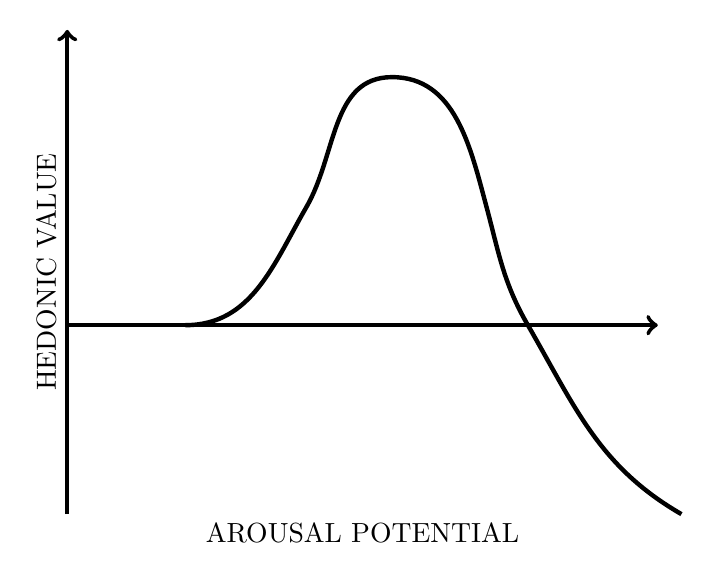
\begin{tikzpicture}[scale=0.75]
      % The image, for reference
      % \node[anchor=south west,inner sep=0] at (0,0) {\includegraphics[width=\textwidth]{wundt.png}};

      % Axes
      \draw[black,ultra thick,->] (1,0.8) -- (1,  9)   node[midway, above, sloped] {HEDONIC VALUE};     % y axis
      \draw[black,ultra thick,->] (1,4)   -- (11, 4);                                                   % x axis
      \path                       (1,0.8) -- (11, 0.8) node[midway, below]         {AROUSAL POTENTIAL}; % x axis label

      % Curve. The numbers come from tracing over wundt.png
      \draw[black,ultra thick] (3, 4)
           to[out=0,   in=240] (5.05, 6)
           to[out=60,  in=180] (6.5,  8.2)
           to[out=0,   in=105] (8.1,  6)
           to[out=-75, in=120] (8.8,  4)
           to[out=-60, in=150] (11.4, 0.8);

      % This version is closer, but a little jagged
      \iffalse
      \draw[black,ultra thick] (3, 4)
           to[out=0,   in=240] (5.05, 6)
           to[out=60,  in=225] (6,    8)
           to[out=45,  in=180] (6.5,  8.2)
           to[out=0,   in=135] (7.2,  8)
           to[out=-45, in=105] (8.1,  6)
           to[out=-75, in=120] (8.8,  4)
           to[out=-60, in=150] (11.4, 0.8);
      \fi
  \end{tikzpicture}

  \caption{The Wundt curve, reproduced from~\cite{berlyne1970novelty}. The axes
    ``hedonic value'' and ``arousal potential'' are described as covering
    \textquote{reward value\dots preference or pleasure}, and \textquote{all the
      stimulus properties that tend to raise arousal, including novelty and
      complexity}, respectively.}
  \label{fig:wundt}
\end{figure}

Another perspective on what is ``interesting'' comes from the artificial
intelligence tasks of optimisation and reinforcement learning. Common pitfalls
for such systems are highly non-convex problems (trapping optimisers in local
minima), and sparse information (such as flat gradients; or highly delayed
rewards, like a single win/lose reward at the end of a game). To mitigate these problems, various forms of internally-generated (or \emph{intrinsic}) rewards
can be incorporated into a system. Such schemes provide reward for interesting
discoveries, which encourages exploration in lieu of external direction, and are
known as \emph{Artificial Curiosity}~\cite{schmidhuber2006developmental} (AC).

The unifying principle of AC methods is to force systems away from data which
are not amenable to learning; either because they are so familiar that there is
nothing left to learn, or so unfamiliar that they are unintelligible. The
resulting behaviour is characterised by the \emph{Wundt curve} (shown in Figure \ref{fig:wundt}) \footnote{In practice, many measures
  avoid negative values for simplicity, in which cases we replace all negative
  points on the curve with zero.}, which has been used in psychology to explain
human aesthetics and preferences \cite{berlyne1970novelty}. This same behaviour
may be applicable to the theorems produced by a theory exploration system.

We can divide AC approaches into two groups: those which make \emph{explicit}
use of interestingness, learning from signals which follow a Wundt curve; whilst
\emph{implicit} approaches modify the \emph{output} of their learning
algorithm(s), to engineer the overall system behaviour to follow a Wundt curve
as an emergent property.

A framework encompassing many examples of the explicit approach is given
in~\cite{oudeyer2007intrinsic} in the context of reinforcement learning; for
comparison, many similar measures are surveyed in a data mining context
in~\cite{geng2006interestingness}. Many more reinforcement learning examples can
be found in~\cite{Kaplan2006, Lipson2007, Luciw2011, Macedo2000,
  Ramik.Sabourin.Madani:2013, Roa.Kruijff.Jacobsson:2009, Schmidhuber:1991,
  oudeyer2004intelligent}; whilst more general descriptions are given
in~\cite{Schaul.Sun.Wierstra.ea:2011, Scott1989, maher2008achieving}, which may
be more amenable to Theory Exploration setting.

Many of these reward signals are based on information theory, with a prominent
example being \emph{compression progress}: given a compressed representation of
our previous observations, the ``progress'' is the space saved if we include the
current observation. Observations which are incompressible or trivially
compressible don't save any space, whilst observations which provide new
insights into the structure of past experience can provide a space saving when
compressed together. This seems particularly relevant for identifying
interesting theorems: those new theorems (``observations'') which shorten the
proofs of previously discovered theorems may be more general, more powerful and
therefore more \emph{interesting}. In fact this is very similar to
\quickspec{}'s interestingness criterion.

Another example of explicit Artificial Curiosity is given
in~\cite{Hester.Stone:2012}, where world states which cause \emph{disagreement}
among a population of decision trees (a \emph{random
  forest}~\cite{randomforests}) are considered interesting. Since the models
make stochastic predictions, the disagreement follows a Wundt curve as the
complexity of state transitions increases: for parts of the state space which
have been fully learned, the models will agree on accurate predictions; for
parts which are unlearnable, the models cannot infer any structure, and will
converge to reporting the same average value. Whilst the latter predictions may
not be \emph{accurate}, they will be \emph{in agreement}, hence pushing down the
interestingness of states which are too complex.

Many examples of the implicit case are based on \emph{coevolution}: rewarding
one part of the system for exploiting another part, and vice versa. In~\cite{Schmidhuber1999} a pair of learning algorithms place virtual ``bets''
on the outcome of actions, and the winner is rewarded at the expense of the
loser. Due to the risk involved, each algorithm will only bet when it is
confident in its prediction, and bets will only be actioned when each algorithm
is confident in a \emph{different} outcome. The overall behaviour of this system
is therefore similar to the explicit measure of disagreement used in the random
forest example.

More recent work on \emph{Generative Adversarial Networks} (GANs) trains a
``discriminator'' program to distinguish real training examples (usually images)
from synthetic data made by a ``generator'' program. Both programs are
differentiable (usually some type of Artificial Neural Network), so the coupling
between the generator's output and the discriminator's input can be used not
only to feed synthetic data ``forwards'', but also to back-propagate the
discriminator's errors (which it is trying to minimise) into the generator
(which then tries to maximise, exploiting the discriminator by synthesising more
realistic data).

Another example of implicit AC is the ``darwinian brain'' of Fernando et
al.~\cite{fernando2013design1, fernando2013design2}. This coevolves a
population of problem generators and problem solvers, rewarding the solvers
based on their speed, and rewarding the generators based on the \emph{variance}
of the solvers' speed. This avoids trivial problems (which all solvers can
quickly overcome) and complex problems (which no solver can manage), and focuses
on those with the most possibility for learning. The role of problem generator
is similar to that of Theory Exploration tools, with solvers being Automated
Theorem Provers.

% TODO Include something about
% variance among experts (decision tree stuff as well as more established
% splitting functions stuff)

% TODO: Also mention the intrinsic reward idea about easily accessible regions
% (e.g. balancing a pole because it's easier to get from there to anywhere else)

% TODO Make sure we mention the recent reinforcement learning task that includes
% a constantly-changing "TV" in the 3D world, shown in some TwoMinutePapers
% videos

An important historical implementation of ATF is Lenat's AM (Automated
Mathematician) system. Unlike prior work, such as
Meta-Dendral~\cite{buchanan:75} and those described in~\cite{winston}, AM aims
to be a general purpose mathematical discovery system, designed to both
construct new concepts and conjecture relationships between them. AM is a
rule-based system which represents knowledge using a frame-like scheme, enlarges
its knowledge base via a collection of heuristic rules, and controls the firing
of these rules via an agenda mechanism. Evaluation of AM considered generality
(performance in new domains) and how finely-tuned various aspects of the program
are (the agenda, the interaction of the heuristics, etc). Most of this
evaluation was qualitative, and has subsequently been
criticised~\cite[chap.~13]{colton:book}. In their case study in methodology,
Ritchie and Hanna found a large discrepancy between the theoretical claims made
of AM and the implemented program~\cite{ritchie1984case}; for example, AM ``invented''
natural numbers from sets, but did so using a heuristic specifically designed to
make this connection.

The prototypical implementation of MTE is the Theorema system of Buchberger and
colleagues~\cite{buchberger,buchberger2016theorema}, which also places a strong
emphasis on user interface and output presentation. Theory exploration in the
Theorema system involves the user formalising their definitions in a consistent,
layered approach; such that reasoning algorithms can exploit this structure in
subsequent proofs, calculations, etc. The potential of this strategy was
evaluated by illustrating the automated synthesis of Buchberger's own Gr\"obner
bases algorithm~\cite{buchberger:04}.

A similar ``layering'' approach is found in the IsaScheme system of
Monta{\~n}o-Rivas \etal{}~\cite{Montano-Rivas.McCasland.Dixon.ea:2012}, which
has also been quantitatively compared against IsaCoSy and HipSpec using
precision/recall analysis~\cite{claessen2013automating}. The name comes from its
embedding in the Isabelle proof assistant and its use of ``schemes'':
higher-order formulae which can be used to generate new concepts and
conjectures. Variables within a scheme are instantiated automatically and this
drives the invention process. For example, the concept of ``repetition'' can be
encoded as a scheme, and instantiated with existing encodings of zero, successor
and addition to produce a definition of multiplication. The same scheme can be
instantiated with this new multiplication function to produce exponentiation.

IsaCoSy and QuickSpec (the conjecture generation component of HipSpec) are
described in more detail in $\S$\ref{sec:existing-tools}, since these are the
tools we chose to evaluate and compare for $\S$\ref{sec:application}. QuickSpec
has since evolved to version 2~\cite{smallbone2017quick}, which replaces the
distinct enumeration and testing steps with a single, iterative algorithm
similar to that of IsaCoSy. Generated conjectures are fed into a Knuth-Bendix
completion algorithm to form a corresponding set of rewrite rules. As
expressions are enumerated, they are simplified using these rules and discarded
if equal to a known expression. If not, QuickCheck tests whether the new
expression can be distinguished from the known expressions through random
testing: those which can are added to the set of known expressions. Those which
cannot be distinguished are conjectured to be equal, and the rewrite rules are
updated.

QuickSpec has also inspired another MTE tool for Haskell called
Speculate~\cite{braquehais2017speculate}, which operates in a similar way but
also makes use of the laws of total orders and Boolean algebra to conjecture
\emph{in}equalities and conditional relations between expressions.

Another notable MTE implementation, distinct from those based in Isabelle and
Haskell, is the MATHsAiD project (Mechanically Ascertaining Theorems from
Hypotheses, Axioms and Definitions)~\cite{roy}. Unlike the tools above, which
generate \emph{conjectures} that may later be sent to automated provers,
MATHsAiD directly generates \emph{theorems}, by making logically valid
inferences from a given set of axioms and definitions. Evaluation of the
interestingness of these theorems was performed qualitatively by the system's
developer, which highlights how these tools could benefit from the availability
of an objective, repeatable, quantitative method of evaluation and comparison
such as ours.

\subsection{Relevance Filtering}
\label{sec:relevance}

The combinatorial nature of formal systems causes many proof search methods,
such as resolution, to have exponential complexity
\cite{haken1985intractability}; hence even a modest size increase can turn a
trivial problem into an intractable one. Finding efficient alternatives for such
algorithms, especially those which are NP-complete (e.g. determining
satisfiability) or co-NP-complete (e.g. determining tautologies), seems
unlikely, as it would imply progress on the famously intractable open problems
of $\text{P} = \text{NP}$ and $\text{NP} = \text{co-NP}$. On the other hand, we
can turn this difficulty around: a modest \emph{decrease} in size may turn an
intractable problem into a solvable one. We can ensure that the solutions to
these reduced problems coincide with the original if we only remove
\emph{redundant} information. This leads to the idea of \emph{relevance
  filtering} (or, \emph{premise selection}, when viewed as the \emph{addition}
of relevant information to an initially-empty problem). This is the core idea
behind our restriction of theory exploration to intelligently-selected clusters
of symbols, rather than whole libraries at a time.

Relevance filtering has mostly been used in automated proof search, where it
simplifies problems by removing from consideration those clauses (axioms,
definitions, lemmas, etc.) which are deemed \emph{irrelevant}. The technique is
used in Isabelle's Sledgehammer tool, during its translation of Isabelle/HOL
theories to statements in first order logic: rather than translating the entire
theory, only a sub-set of relevant clauses are included. This reduces the size
of the problem and speeds up the proof search, but it creates the new problem of
determining when a clause is relevant: how do we know what will be required,
before we have the proof?

The initial approach taken by Sledgehammer, known as \textsc{MePo} (from
\emph{Meng-Paulson} \cite{meng2009lightweight}), gives each clause a score
based on the proportion $\frac{m}{n}$ of its symbols which are ``relevant''
(where $n$ is the number of symbols in the clause and $m$ is the number which
are relevant). Initially, the relevant symbols are those which occur in the goal
to be proved, but whenever a clause is found which scores more than a particular
threshold, all of its symbols are then also considered relevant. There are other
heuristics applied too, such as increasing the score of user-provided facts
(e.g. given by keywords like \texttt{using}), locally-scoped facts, first-order
facts and rarely-occuring facts. To choose $r$ relevant clauses for an ATP
invocation, we simply order the clauses by decreasing score and take the first
$r$ of them.

Recently, a variety of alternative algorithms have also been investigated, for
example the \textsc{MaSH} algorithm (Machine Learning for SledgeHammer)
\cite{kuhlwein2013mash} uses the ``visibility'' of one theorem from another to
determine the relevance of clauses. Visibility is essentially a dependency graph
of which theorems were used in the proofs of which other theorems (although the
theorems are actually represented as abstract sets of features). To select
relevant clauses for a goal, the set of clauses which are visible from the
goal's components is generated; this is further reduced by (an efficient
approximation of) a na\"{\i}ve Bayes algorithm.

Another example is \emph{multi-output ranking} (MOR), which uses a support
vector machine (SVM) approach for selecting relevant axioms from the Mizar
Mathematical Library for use by the Vampire ATP system
\cite{alama2014premise}. Many more approaches are described and evaluated in
\cite{kuhlwein2012overview}, some of which may be directly applicable in the
context of theory exploration.


\section{Background}
\label{sec:background}

\subsection{Haskell}
\label{sec:haskell}

\begin{figure}
  \begin{equation*}
    \begin{split}
      expr\    \rightarrow\ & \texttt{Var}\ id                                       \\
                         |\ & \texttt{Lit}\ literal                                  \\
                         |\ & \texttt{App}\ expr\ expr                               \\
                         |\ & \texttt{Lam}\ \mathcal{L}\ expr                        \\
                         |\ & \texttt{Let}\ bind\ expr                               \\
                         |\ & \texttt{Case}\ expr\ \mathcal{L}\ \left[ alt \right]   \\
                         |\ & \texttt{Type}                                          \\
      id\      \rightarrow\ & \texttt{Local}\ \mathcal{L}                            \\
                         |\ & \texttt{Global}\ \mathcal{G}                           \\
      literal\ \rightarrow\ & \texttt{LitNum}\ \mathcal{N}                           \\
                         |\ & \texttt{LitStr}\ \mathcal{S}                           \\
      alt\     \rightarrow\ & ( altcon,\ [\mathcal{L}],\ expr )                      \\
      altcon\  \rightarrow\ & \texttt{DataAlt}\ \mathcal{G}                          \\
                         |\ & \texttt{LitAlt}\ literal                               \\
                         |\ & \texttt{Default}                                       \\
      bind\    \rightarrow\ & \texttt{NonRec}\ \mathcal{L}\ expr                     \\
                         |\ & \texttt{Rec}\ [ ( \mathcal{L},\ expr ) ]
    \end{split}
  \end{equation*}
  Where:
  \begin{tabular}[t]{l @{ $=$ } l}
    $\mathcal{S}$ & string literals    \\
    $\mathcal{N}$ & numeric literals   \\
    $\mathcal{L}$ & local identifiers  \\
    $\mathcal{G}$ & global identifiers
  \end{tabular}

  \caption{Simplified syntax of GHC Core in BNF style. $[]$ and $(,)$ denote repetition and grouping, respectively.}
  \label{fig:coresyntax}
\end{figure}

We decided to focus on theory exploration in the Haskell programming language as it has mature, state-of-the-art implementations (\qspec{} \citep{QuickSpec} and \hspec{} \citep{claessen2013automating}). This is evident from the fact that the state-of-the-art equivalent for Isabelle/HOL, the \textsc{Hipster} \citep{Hipster} system, is actually implemented by translating to Haskell and invoking \hspec{}.

Haskell is well-suited to programming language research; indeed, this was a goal of the language's creators \citep{marlow2010haskell}. Like most members of the \emph{functional programming} paradigm, Haskell is essentially a variant of $\lambda$-calculus, with extra features such as a strong type system and ``syntactic sugar'' to improve readability. For simplicity, we will focus on an intermediate representation of the \textsc{GHC} compiler, known as \emph{GHC Core}, rather than the relatively large and complex syntax of Haskell proper. Core is based on \fc{}, but for our machine learning purposes we are mostly interested in its syntax; for a more thorough treatment of \fc{} and its use in GHC, see \citep[Appendix C]{sulzmann2007system}.

The sub-set of Core we consider is shown in figure \ref{fig:coresyntax}; compared to the full language \footnote{As of GHC version 7.10.2, the latest at the time of writing.} our major changes are to ignore type hints (explicit casts are removed, whilst particular types/kinds/coercions are all represented by \texttt{Type}) and to use a custom representation of names. We also omit several other forms of literal (machine words of various sizes, individual characters, etc.) for brevity, as their treatment is similar to those of strings and numerals.

\subsection{QuickCheck}
\label{sec:quickcheck}

Although unit testing is the de facto industry standard for quality assurance in non-critical systems, the level of confidence it provides is rather low, and totally inadequate for many (e.g. life-) critical systems. To see why, consider the following Haskell function, along with some unit tests:

\begin{lstlisting}[language=Haskell, xleftmargin=.2\textwidth, xrightmargin=.2\textwidth]
factorial 0 = 1
factorial n = n * factorial (n-1)

fact_base      = factorial 0 == factorial 1
fact_increases = factorial 3 <= factorial 4
fact_div       = factorial 4 == factorial 5 `div` 5
\end{lstlisting}

The intent of the function is to map an input $n$ to an output $n!$. The tests check a few properties of the implementation, including the base case, that the function is monotonically increasing, and a relationship between adjacent outputs. However, these tests will \emph{not} expose a serious problem with the implementation: it diverges on half of its possible inputs!

All of Haskell's built-in numeric types allow negative numbers, which this implementation doesn't take into account. Whilst this is a rather trivial example, it highlights a common problem: unit tests are insufficient to expose incorrect assumptions. In this case, our assumption that numbers are positive has caused a bug in the implementation \emph{and} limited the tests we've written.

If we do manage to spot this error, we might capture it in a \emph{regression test} and update the definition of \hs{factorial} to handle negative numbers, e.g. by taking their absolute value:

\begin{lstlisting}[language=Haskell, xleftmargin=.2\textwidth, xrightmargin=.2\textwidth]
factorial 0 = 1
factorial n = let nPos = abs n
               in nPos * factorial (nPos - 1)

fact_neg = factorial 1 == factorial (-1)
\end{lstlisting}

However, this is \emph{still} not enough, since this function will also accept fractional values\footnote{Since we only use generic numeric operations, the function will be polymorphic with a type of the form \hs{forall t. Num t => t -> t}, where \hs{Num t} constrains the type variable \hs{t} to be numeric. In fact, Haskell will infer extra constraints such as \hs{Eq t} since we have used \hs{==} in the unit tests.}, which will also cause it to diverge. Clearly, by choosing what to test we are biasing the test suite towards those cases we've already taken into account, whilst neglecting the problems we did not expect.

Haskell offers a partial solution to this problem in the form of \emph{property checking}. Tools such as \qcheck{} separate tests into three components: a \emph{property} to check, which unlike a unit test may contain \emph{free variables}; a source of values to instantiate these free variables; and a stopping criterion. Here is how we might restate our unit tests as properties:

\begin{lstlisting}[language=Haskell, xleftmargin=.2\textwidth, xrightmargin=.2\textwidth]
fact_base        = factorial 0 == factorial 1
fact_increases n = factorial n <= factorial (n+1)
fact_div       n = factorial n == factorial (n+1) `div` (n+1)
fact_neg       n = factorial n == factorial (-n)
\end{lstlisting}

The free variables (all called \hs{n} in this case) are abstracted as function parameters; these parameters are implicitly \emph{universally quantified}, i.e. we've gone from a unit test asserting $factorial(3) \leq factorial(4)$ to a property asserting $\forall n, factorial(n) \leq factorial(n+1)$. Notice that unit tests like \hs{fact_base} are valid properties; they just assert rather weak statements.

To check these properties, \qcheck{} treats closed terms (like \hs{fact_base}) just like unit tests: pass if they evaluate to \hs{True}, fail otherwise. For open terms, a random selection of values are generated and passed in via the function parameter; the results are then treated in the same way as closed terms. The default stopping criterion for \qcheck{} (for each test) is when a single generated test fails, or when 100 generated tests pass.

The ability to state \emph{universal} properties in this way avoids some of the bias we encountered with unit tests. In the \hs{factorial} example, this manifests in two ways:

\begin{itemize}
  \item \qcheck{} cannot test polymorphic functions; they must be \emph{monomorphised} first (instantiated to a particular concrete type). This is a technical limitation, since \qcheck{} must know which type of values to generate, but in our example it would bring the issue with fractional values to our attention.

  \item The generators used by \qcheck{} depend only on the \emph{type} of value they are generating: since \hs{Int} includes positive and negative values, the \hs{Int} generator will output both. This will expose the problem with negative numbers, which we weren't expecting.
\end{itemize}

Property checking is certainly an improvement over unit testing, but the problem of tests being biased towards expected cases remains, since we are manually specifying the properties to be checked.

We can reduce this bias further through the use of \emph{theory exploration} tools, such as \qspec{} and \hspec{}. These programs \emph{discover} properties of a ``theory'' (e.g. a library), through a combination of brute-force enumeration, random testing and (in the case of \hspec{}) automated theorem proving.

\subsection{Theory Exploration}
\label{sec:theoryexploration}

\newcommand{\blank}{\cdot}

In this work we consider the problem of \emph{(automated) theory exploration}, which includes the ability to \emph{generate} conjectures about code, to \emph{prove} those conjectures, and hence output \emph{novel} theorems without guidance from the user. The method of conjecture generation is a key characteristic of any theory exploration system, although all existing implementations rely on brute force enumeration to some degree.

We focus on \qspec{} \citep{QuickSpec}, which conjectures equations about Haskell code (these may be fed into another tool, such as \hspec{}, for proving). These conjectures are arrived at through the following stages:

\begin{enumerate}
  \item Given a typed signature $\Sigma$ and set of variables $V$, \qspec{} generates a list $terms$ containing the functions and constants from $\Sigma$, the variables from $V$ and type-correct function applications $f(x)$, where $f$ and $x$ are elements of $terms$. To ensure the list is finite, function applications are only nested up to a specified depth (by default, 3).
  \item The elements of $terms$ are grouped into equivalence classes, based on their type.
  \item Each variable is instantiated to a particular value, generated randomly by \qcheck{}.
  \item For each class, the members are compared (using a pre-specified function, such as equality \hs{==}) to see if these instantiations have caused an observable difference between members. If so, the class is split up to separate such distinguishable members.
  \item The previous steps of variable instantiation and comparison are repeated until the classes stabilise (i.e. no differences have been observed for some specified number of repetitions).
  \item A set of equations are then conjectured, relating each class's members.
\end{enumerate}

Such $conjectures$ can be used in several ways: they can be simplified for direct presentation to the user (by removing any equation which can be derived from the others by rewriting), sent to a more rigorous system like \hspec{} or \textsc{Hipster} for proving, or even serve as a background theory for an automated theorem prover \citep{claessen2013automating}.

As an example, we can consider a simple signature for Peano numerals, addition and multiplication:

\begin{align*}
  \Sigma_{\mathbb{N}} = \{ & 0     && : \mathbb{N}, \\
                        & succ  && : \mathbb{N} \rightarrow \mathbb{N}, \\
                        & plus  && : \mathbb{N} \rightarrow \mathbb{N} \rightarrow \mathbb{N}, \\
                        & times && : \mathbb{N} \rightarrow \mathbb{N} \rightarrow \mathbb{N}\}
\end{align*}

Together with a set of variables, say $V_{\mathbb{N}} = \{x, y, z\}$, \qspec{}'s enumeration will resemble the following:

\begin{align*}
  terms_{\mathbb{N}} = [& 0,\ succ,\ plus,\ times,\ x,\ y,\ z,\ succ(0),\ succ(x),\ succ(y), \\
                     & succ(z),\ plus(0,\blank),\ plus(x, \blank),\ \dots ]
\end{align*}

Notice that our functions are curried, where $f(x,\blank)$ indicates \emph{partial application} of $f$ to $x$. This is required as the construction of $terms$ applies functions to one argument at a time.

\begin{figure}
  % To reproduce, run 'quickSpec nat' in haskell_example/src/QuickSpecExample.hs
  \begin{align*}
                        plus(x, y) &= plus(y, x)            \\
                        plus(x, 0) &= x                     \\
               plus(x, plus(y, z)) &= plus(y, plus(x, z))   \\
                       times(x, y) &= times(y, x)           \\
                       times(x, 0) &= 0                     \\
             times(x, times(y, z)) &= times(y, times(x, z)) \\
                  plus(x, succ(y)) &= succ(plus(x, y))      \\
                 times(x, succ(y)) &= plus(x, times(x, y))  \\
              times(x, plus(y, y)) &= times(y, plus(x, x))  \\
    plus(times(x, y), times(x, z)) &= times(x, plus(y, z))
  \end{align*}
  \caption{Equations conjectured by \qspec{} for Peano numerals, addition and multiplication; after simplification.}
  \label{fig:qspecresult}
\end{figure}

These terms will be grouped into three classes, one each for $\mathbb{N}$, $\mathbb{N} \rightarrow \mathbb{N}$ and $\mathbb{N} \rightarrow \mathbb{N} \rightarrow \mathbb{N}$. As the variables $x$, $y$ and $z$ are instantiated to various randomly-generated numbers, these equivalence classes will be divided, until eventually the equations in figure \ref{fig:qspecresult} are conjectured.

Although complete, this enumeration approach is wasteful: many terms are unlikely to appear in theorems, which requires careful choice by the user of what to include in the signature. Here we know that addition and multiplication are closely related, and hence obey many algebraic laws. Our machine learning technique aims to predict these kinds of relations between functions, so we can create small signatures which nevertheless have the potential to give rise to many equations.

\qspec{} (and \hspec{}) are also compatible with Haskell's existing testing infrastructure, such that an invocation of \texttt{cabal test} can run these tools alongside more traditional QA tools like \qcheck{}, \textsc{HUnit} and \textsc{Criterion}.

In fact, there are similarities between the way a TE system like \qspec{} can generalise from checking \emph{particular} properties to \emph{inventing} new ones, and the way counterexample finders like \qcheck{} can generalise from testing \emph{particular} expressions to \emph{inventing} expressions to test. One of our aims is to understand the implications of this generalisation, the lessons that each can learn from the other's approach to term generation, and the consequences for testing and QA in general.

\subsection{Clustering and Feature Extraction}
\label{sec:featureextraction}

Our approach to scaling up these Haskell theory exploration tools takes inspiration from two sources. The first is premise selection, which makes expensive algorithms used in theorem proving more practical by limiting the size of their inputs. We describe this approach in more details in \S \ref{sec:relevance}. Premise selection is a practical tool, used in production systems like the \emph{Sledgehammer} component of the Isabelle/HOL theorem prover.

Despite the idea's promise, we cannot simply invoke existing premise selection algorithms in our theory exploration setting. The reason is that theory exploration has no distinct \emph{goal} to compare expressions against. Instead, we are interested in relationships between \emph{any} terms generated from a signature, and hence we must consider the relevance of \emph{all terms} to \emph{all other terms}. A natural fit for such problems is \emph{clustering}, which attempts to group similar inputs together in an unsupervised way. See \S \ref{sec:clustering} for more information.

Our hypothesis is that clustering methods, as found in systems like ML4PG and ACL2(ml), can be used as relevance filters to break up large signatures into smaller ones more amenable to brute force enumeration.

\iffalse TODO: I would play up the clustering intelligence. Clustering is not just about breaking up, it is about discovering significant patterns in data. By forgetting this, you make motivation for your work sound too ``small'' \fi

Both of these approaches, premise selection and clustering, use \emph{machine learning} (ML) algorithms to analyse expressions, and hence rely on \emph{feature extraction} to transform the data into a suitable representation and remove irrelevant details. This has two benefits:

\begin{itemize}
  \item \emph{Feature vectors} (ordered lists of features) are chosen to represent the relevant information in a more compressed form than the raw data (for example, replacing descriptive identifier names with sequential numbers). This reduces the input size of the machine learning problem, improving efficiency (e.g. running time).
  \item We avoid learning irrelevant details, such as the text encoding system used, improving \emph{data} efficiency (the number of samples required to spot a pattern).
\end{itemize}

Another benefit of feature extraction is to \emph{normalise} the input data to a fixed-size representation. Many ML algorithms only work with inputs of a uniform size; feature extraction allows us to use these algorithms in domains where the size of each input is not known, may vary or may even be unbounded.

In our case, we will use a novel feature extraction algorithm, described in \S \ref{sec:recurrentclustering}, to transform expressions in Haskell Core into a fixed size representation, suitable for clustering via the standard \emph{k-means} algorithm.

\iffalse TODO: I have had a look now at section 5. I do not think feature extraction and clustering is explained/defined there, either. Seeing your contribution is feature extraction algorithms, you need to define feature vectors and clusters *here* \fi

\iffalse

\begin{figure}
  \centering
  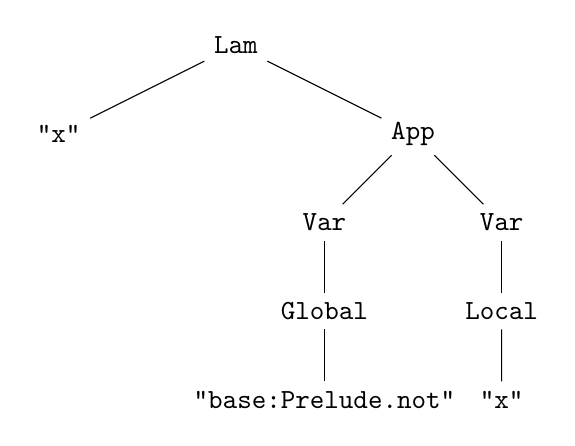
\begin{tikzpicture}[scale=0.75, level/.style={sibling distance=60mm/#1}]
      % Tree
      \node {\texttt{Lam}}
        child {node {\texttt{"x"}}}
        child {node {\texttt{App}}
          child {node {\texttt{Var}}
            child {node {\texttt{Global}}
              child {node {\texttt{"base:Prelude.not"}}}}}
          child {node {\texttt{Var}}
            child {node {\texttt{Local}}
              child {node {\texttt{"x"}}}}}};

      % Arrow
      %\node[single arrow,
      %      draw=black,
      %      fill=black!10,
      %      minimum height=2cm,
      %      shape border rotate=0] at (0,-1) {};
      %\draw[-latex] (A.east) -- (B.west);

      % Feature vector

  \end{tikzpicture}

  \caption{}

  \label{fig:featureextractionpic}
\end{figure}

\subsection{Clustering}
\label{sec:clustering}
% TODO
\fi

\chapter{Theory Exploration Benchmark}
\label{sec:benchmark}

If we wish to make measurable progress on the task of conjecture generation, we
must quantify what it is we are trying to achieve. Various approaches can then
be measured and compared to optimise toward our goal. To this end we define a
benchmarking methodology, shown in Figure~\ref{fig:flow_chart} on
page~\pageref{fig:flow_chart}, which both generates a large
definition/ground-truth corpus, and provides a scalable, statistical approach to
evaluating MTE tools using this corpus. We follow a precision/recall approach
similar to prior work, with the main difference being the source of definitions
and ground truths: we take existing problem sets designed for automated theorem
proving, and adapt their content for use in the conjecture generation setting.

\section{Preparation}
\label{section:prep}

Automated theorem proving is an active area of research, with large problem sets
and regular competitions to prove as much as possible, as fast as
possible~\cite{pelletier2002development}. These problem sets are an opportunity
for MTE, as their definitions and theorems can be used as a corpus in the same
way that Isabelle libraries have been used in the past.

Some problem sets are more amenable for this purpose than others. The most
suitable are those meeting the following criteria:

\begin{itemize}
\item For each problem, there should be a clear distinction between the
  statement to be proved and the definitions involved, such that the two can be
  easily and meaningfully separated. This rules out problem sets like those of
  SMT-COMP~\cite{barrett2005smt}, where many problems involve uninterpreted
  functions, whose behaviour is \emph{implicit} in the logical structure of the
  theorem statement but not separately \emph{defined}.
\item Definitions should be translatable into a form suitable for the MTE tools
  under study. Our application in $\S$\ref{sec:application} requires Haskell and
  Isabelle translations, and also benefits from having definitions be strongly
  typed.
\item The problem set should be relevant to the desired domain. Our focus on
  functional programming requires higher-order functions and inductively defined
  datatypes, which rules out first-order languages/logics (such as
  TPTP~\cite{sutcliffe2009tptp}).
\item The problem set should ideally contain \emph{every} ``interesting''
  property involving its included definitions, since non-membership in the
  ground truth will be treated as being ``uninteresting''. More realistically,
  we should aim for each definition to have \emph{multiple} properties; rather
  than a mixture of unrelated problems, cherry-picked from different domains.
\item Larger problem sets are preferable as they give more robust statistics, all
  else being equal (i.e. when this does not sacrifice quality).
\end{itemize}

Once such a problem set has been chosen, we must separate the definitions from
the theorem statements which reference those definitions. The definitions will
be used as input to the MTE tools, whilst the theorem statements form the ground
truth corpus of properties (which tool output will be compared against).

It is important to ensure that there are no duplicate definitions: we are only
concerned with the \emph{logical} content of the input, not the more arbitrary
aspects of their presentation like the names of functions. For example, consider
a problem set which includes a statement of commutativity for a \texttt{plus}
function, and of associativity for an \texttt{add} function, where the
definitions of \texttt{plus} and \texttt{add} are $\alpha$-equivalent. We would
expect an MTE tool to either conjecture commutativity and associativity for
\emph{both} functions, or for \emph{neither} function, since they are logically
equivalent. Yet a na\"ive precision/recall analysis would treat commutativity of
\texttt{add} and associativity of \texttt{plus} as \emph{uninteresting}, since
they don't appear in the ground truth.

For this reason, duplicates should be removed, and any references to them
updated to use the remaining definition (e.g. chosen based on lexicographic
order). In the above example, the \texttt{plus} function would be removed, and
the commutativity statement updated to reference \texttt{add} instead.

\section{Sampling}
\label{section:sampling}

We could, in theory, send these de-duplicated definitions straight into an MTE
tool and use the entire set of properties (taken from the theorem statements) as
the ground truth for analysis. However, this would cause two problems:

\begin{itemize}
\item The result would be a single data point, which makes it difficult to
  infer performance \emph{in general}.
\item It is impractical to run existing MTE tools on inputs containing more
  than a few dozen definitions.
\end{itemize}

To solve both of these problems we instead \emph{sample} a subset of
definitions.\footnote{This could be done randomly, but for reproducibility we
  use a deterministic order based on cryptographic hashes.} Given a sample size,
we choose a subset of that many definitions, and provide only those as input to
the tool. We generate a corresponding ground truth by selecting those properties
from the corpus which ``depend on'' (contain references to) \emph{only} the
definitions in that sample. Transitive dependencies aren't required (e.g. a
property involving only a \texttt{times} function would not depend on a
\texttt{plus} function, even if \texttt{plus} occurs in the definition of
\texttt{times}).

Unfortunately, uniform sampling of definitions gives rise to a lottery: for a
given sample size, increasing the size of the corpus (which provides better
statistics) makes it less likely that a chosen sample will contain all of
a property's dependencies. The majority of such samples would hence have an
empty ground truth, and thus $0$ precision and undefined recall
\emph{independent} of the tool's output! This is clearly undesirable as an
evaluation method.

Other measurements could be used for such cases, but our approach is to avoid
them by only allowing a sample if it contains all dependencies of at least one
property. We could do this using rejection sampling, but it is more efficient to
pick a property, weighted in proportion to their number of dependencies
(ignoring those with more dependencies than our sample size). That property's
dependencies become our sample, padded up to the required size with uniform
choices from the remaining definitions.

The ground truth for such samples is guaranteed to contain at least one property
(the one we picked), and hence the precision and recall will depend meaningfully
on the tool's output. One downside of this restriction is that we limit the
number of possible samples to measure; this is significant for sample sizes less
than 3.

\section{Evaluation}
\label{section:evaluation}

Given a sample of definitions and a corresponding ground truth, the actual
execution of the MTE tool proceeds as in prior work. We must translate the
chosen definitions into the required input format, then we time the execution
with a timeout (e.g. 5 minutes). We use wall-clock time since
\begin {enumerate*} [i) ]%
\item this is most relevant to a user's experience,
\item it has a straightforward interpretation and
\item measuring it does not require intrusive alterations to a tool's
  implementation.
\end {enumerate*}
The downside is that comparisons must take hardware performance into account,
which would not be the case if time were measured by some proxy like number of
expressions evaluated.

In our experiments we have found that memory usage is also an important part of
a tool's performance, but rather than complicating our analysis with an extra
dimension, we instead allow programs to use as much memory as they like, and
either get killed by the operating system or slow down so much from swapping
that they time out. This is in line with the expected usage of these tools:
either there is enough memory, or there isn't; implementations shouldn't be
penalised for making use of available resources.

To calculate precision and recall, the conjectures generated by each tool, as
well as the ground-truth properties, need to be parsed into a common format and
compared syntactically after normalising away ``irrelevant'' details. We
consider variable naming to be irrelevant, which can be normalised by numbering
free variables from left to right and using de Bruijn indices for bound
variables. We also consider the left/right order of equations to be irrelevant,
which we normalise by choosing whichever order results in the
lexicographically-smallest expression.

We specifically \emph{ignore} other logical relationships between syntactically
distinct statements, such as one equation being implied by another. Whilst
logically sound, second-guessing the ground truth in this way would harm other
aspects which influence interestingness (for example, a more general statement
is more widely applicable, but it might also be harder to comprehend).

This procedure gives us a single runtime, precision and recall value for each
sample. We propose two methods for analysing this data: \emph{summarising}
the performance of a single MTE tool and \emph{comparing} the performance of two
tools.

\subsection{Summarising}

Each sample is only explored once by each tool, so that we cover as many
independent samples as possible to better estimate how a tool's performance
generalises to unseen inputs. How we combine these data into an aggregate
summary depends on what we are interested in measuring. One general question we
might ask is how a tool's performance scales with respect to the input size (the
number of given definitions). This is straightforward to measure by varying the
sample size, but we need some way to combine the results from samples of the
same size.

We can summarise a set of runtimes by choosing the median, as this is more
robust than the mean against long-running outliers, and hence represents
performance for a ``typical'' input of that size. Since our methodology measures
performance over many samples, we can also compute the \emph{spread} of our
data, for example the inter-quartile range. This is not possible using the
one-off measurements common in prior evaluation methods.

Considering precision and recall separately, there are two ways to average these
for a set of samples. Since both of these measurements are ratios, their means
are known as the \emph{average of the ratios} (AOR). Using the definitions of
precision and recall given in $\S$\ref{sec:te}, we can define the average of the
ratios for $S$ samples indexed by $1 \leq i \leq S$ as follows:

\begin{align*}
       \overline{\text{precision}}_{AOR}
    &= \frac{1}{S} \sum_i{\text{precision}_i} \\
    &= \frac{1}{S} \sum_i{
         \frac{\#\text{interesting}_i}
              {\#\text{generated}_i}}         \\[10pt]
       \overline{\text{recall}}_{AOR}
    &= \frac{1}{S} \sum_i{\text{recall}_i} \\
    &= \frac{1}{S} \sum_i{
         \frac{\#\text{interesting}_i}
              {\#\text{groundtruth}_i}}
\end{align*}

We interpret these mean values as the \emph{expected} precision and recall for
samples of this size. In particular, these tell us the quality of the \emph{set}
of conjectures that will be generated if we were to run the tool on such a
sample, but they don't give us direct information about the individual
conjectures themselves. Since these are mean values, they are the reference
point for measures of spread such as the variance, standard deviation and mean
absolute deviation.

The alternative is to calculate \emph{pooled} averages, by combining the
(multi)sets from each sample before taking the ratios. The size of these pooled
sets is simply the sum of the individual set sizes, and ratios of these sums are
equal to ratios of the means (since the normalising factor $\frac{1}{S}$ appears
in both numerator and denominator). Hence these values are known as the
\emph{ratio of the averages} (ROA):

\begin{align*}
       \overline{\text{precision}}_{ROA}
    &= \frac{\sum_i{\#\text{interesting}_i}}
            {\sum_i{\#\text{generated}_i}}                              \\
    &= \frac{\frac{1}{S} \sum_i{\#\text{interesting}_i}}
            {\frac{1}{S} \sum_i{\#\text{generated}_i}}                  \\
    &= \frac{\hspace{5pt} \overline{\#\text{interesting}} \hspace{5pt}}
            {\hspace{5pt} \overline{\#\text{generated}}   \hspace{5pt}} \\[10pt]
       \overline{\text{recall}}_{ROA}
    &= \frac{\sum_i{\#\text{interesting}_i}}
            {\sum_i{\#\text{groundtruth}_i}}                            \\
    &= \frac{\frac{1}{S} \sum_i{\#\text{interesting}_i}}
            {\frac{1}{S} \sum_i{\#\text{groundtruth}_i}}                \\
    &= \frac{\hspace{5pt} \overline{\#\text{interesting}} \hspace{5pt}}
            {\hspace{5pt} \overline{\#\text{groundtruth}} \hspace{5pt}}
\end{align*}

Larger sets contribute more to a ratio of averages, unlike the mean which treats
each set equally. This weighting gives us expected qualities of
\emph{conjectures} rather than sets: the ROA for precision is the expected
chance that some particular generated conjecture will appear in the ground
truth; the ROA for recall is the expected chance that some particular ground
truth property will appear in the generated output.

These averages can differ when there is a large variation in set size. For
example, if we generate a single, interesting conjecture for one sample and 99
uninteresting conjectures for another sample, the AOR (mean) precision will be
$\frac{1}{2}$ but the ROA precision will be $\frac{1}{100}$. This highlights the
importance of knowing \emph{absolute} numbers of conjectures, such as the mean
output size $\overline{\#\text{generated}}$ and its spread, alongside the
proportions given by precision and recall.

It is also possible to combine precision values \emph{with} recall values
(either individually or aggregated) by calculating their \emph{F-score}, defined
as:

\begin{equation*}
  F = 2 \times \frac{\text{precision} \times \text{recall}}
                    {\text{precision} +      \text{recall}}
\end{equation*}

This is the harmonic mean of precision and recall, ranging between 0 and 1. The
F-score summarises performance into a single number, which is useful for
purposes like ranking, but it obscures insights we might gain from looking at
precision and recall separately (e.g. whether a tool is generating too much
output or too little).

\subsection{Comparison}

To measure progress and encourage competition in the field, it is important to
compare the relative performance of different tools on the same task. Since the
aggregate statistics in the above summaries have obscured the details of
specific runs, any comparison based on them (such as comparing mean recall)
would have very low statistical power. More direct comparisons can be made using
\emph{paired} tests, since for each individual sample we have measurements for
\emph{both} tools.

Running times do not follow a normal distribution, in particular due to the
lower bound at 0, which complicates any application of standard comparisons like
the paired z-test. An alternative which does not assume normality is the
Wilcoxon signed-rank test~\cite{wilcoxon1945individual}, which has been applied
to software benchmarking in the Speedup-Test protocol of Touati, Worms and
Briais~\cite{touati2013speedup}. Our methodology differs by measuring with a
different sample each time, rather than repeatedly measuring one sample of each
size; this also allows us to use the paired form of the Wilcoxon test.

Another complication with our time measurements is the censoring effect caused
by timeouts. Paired difference tests are robust to this, since the upper-bound
on total time imposes an upper-bound to the observable difference; this biases
our results in a conservative way, \emph{towards} the null hypothesis of
indistinguishable performance.

Quality can be compared using precision and recall, but we must choose how to
handle samples where one tool succeeded and the other failed (e.g. timing out).
One approach would be to consider failed runs as if they generated an empty set
of conjectures; this conflates quality with failure, which may be desirable, but
we prefer the more charitable approach of comparing only those samples where
both tools finished successfully. We pool the results from such samples together
(allowing duplicates) and compare the resulting proportions.

Recall relies on a fixed set of properties, the ground truth, so we can compare
tools using McNemar's test for paired samples~\cite{mcnemar1947note}. For each
tool, we count how many of the ground-truth properties it found which were
\emph{not} found by the other tool. McNemar's test determines whether we can
reject the null hypothesis that both tools have the same count (i.e. both tools
have a similar contribution to the symmetric difference of their interesting
outputs).

Comparing precision cannot be done in the same way as recall, since we do not
have a fixed set of properties to divide up (there are an unlimited number of
properties that may or may not appear in a tool's output). Instead, we can count
how many conjectures were interesting and uninteresting for each tool and use
Boschloo's form of Barnard's test~\cite{lydersen2009recommended} to determine if
these proportions are independent. This assumes a binomial distribution and is
conditioned on the number of generated conjectures (as if this were fixed by
design).

\begin{figure}
  \tikzstyle{startstop} = [rectangle, rounded corners, minimum width=3cm,
                           minimum height=1cm,text centered, draw=black]

  \tikzstyle{io} = [trapezium, trapezium left angle=70,
                    trapezium right angle=110, minimum width=1cm,
                    minimum height=1cm, text centered, draw=black]

  \tikzstyle{process} = [rectangle, minimum width=3cm, minimum height=1cm,
                         text centered, draw=black]
  \tikzstyle{decision} = [diamond, minimum width=3cm, minimum height=1cm,
                          text centered, draw=black]

  \tikzstyle{arrow} = [thick,->,>=stealth]

  % Avoids too much padding in io shapes
  \tikzset{trapezium stretches=true}

  \centering
  \scalebox{0.9}{\begin{tikzpicture}[node distance=1cm]

    % Preparation section

    \node (in)  [io]{Theorem Proving Benchmark};
    \node (sep) [process,       below=1cm of in         ]{Separate definitions from property statements};
    \node (def) [process, below  left=1.5cm and -1cm of sep]{Remove duplicate definitions};
    \node (ref) [process, below right=1.5cm and -1cm of sep]{Update references};

    \node (thy)  [startstop, below=1cm of def]{Distinct Definitions};
    \node (thm)  [startstop, below=1cm of ref]{Corpus of Properties};

    \draw [arrow] (in)  -- (sep);
    \draw [arrow] (def) -- (ref);
    \draw [arrow] (def) -- (thy);
    \draw [arrow] (ref) -- (thm);

    % Arrows with labels
    \path[->]
        (sep) edge [arrow, sloped, above] node {definitions} (def)
        (sep) edge [arrow, sloped, above] node {properties}  (ref);

    % Sampling section

    \node (choose) [process, below=of thm   ]{Choose a property};
    \node (deps)   [process, below=of choose]{List property's dependencies};

    % Create dummy coordinate below deps, then use its y coordinate for pad
    \coordinate [below=of deps] (padDummy);
    \path let \p{dummy} = (padDummy),
              \p{in}    = (in)
              in coordinate (padPos) at (\x{in}, \y{dummy});
    \node (pad)  [process, at=(padPos)]{Pad list to form sample};

    \node (sthm) [startstop, below right=1.5cm and -1cm of pad]{Ground Truth};
    \node (sthy) [startstop, below  left=1.5cm and -1cm of pad]{Sampled Theory};


    % Calculate position of (size) using let, then define as normal
    \path let \p{pad}    = (pad),
              \p{choose} = (choose)
           in coordinate (sizePos) at (\x{pad},\y{choose});
    \node (size) [io, at=(sizePos)] {Sample size};

    % Evaluation section
    \path let \p{pad}  = (pad),
              \p{sthm} = (sthm)
           in coordinate (runPos) at (\x{pad}, \y{sthm});
    \node (run) [process, below=of runPos]{Run MTE tool};
    \node (pr)  [process, below=of run]{Analysis};

    \node (prec) [startstop, below=of pr  ]{Precision};
    \node (time) [startstop,  left=of prec]{Time taken};
    \node (rec)  [startstop, right=of prec]{Recall};

    \draw [arrow] (thy)    |- (pad);
    \draw [arrow] (thm)    -- (choose);
    \draw [arrow] (choose) -- (deps);
    \draw [arrow] (deps)   |- (pad);
    \draw [arrow] (size)   -- (choose);
    \draw [arrow] (size)   -- (pad);
    \draw [arrow] (pad)    -- (sthm);
    \draw [arrow] (pad)    -- (sthy);
    \draw [arrow] (sthy)   |- (run);
    \draw [arrow] (run)    -- (pr);
    \draw [arrow] (sthm)   |- (pr);
    \draw [arrow] (pr)     -- (prec);
    \draw [arrow] (pr)     -- (rec);
    \draw [arrow] (pr)     -- (time);

    % Awkward arrow
    \draw [arrow] (thm) -| ([shift={(7mm,-7mm)}]thm.east) |- (sthm);

    % Braces

    % Preparation
    \draw
      let \p{thm} = (thm.east),
          \p{in}  = (in.north),
          \p{rec} = (rec.south east)
       in [decorate,decoration={brace, amplitude=10pt}, xshift=0.5cm]
       (\x{rec}, \y{in}) -- (\x{rec}, \y{thm})
         node [black, midway, right, xshift=0.3cm]
              {Preparation $\S$\ref{section:prep}};

    % Sampling
    \draw
      let \p{thm} = (thm.east),
          \p{gt}  = (sthm.east),
          \p{rec} = (rec.south east)
       in [decorate,decoration={brace, amplitude=10pt}, xshift=0.5cm]
       (\x{rec}, \y{thm}) -- (\x{rec}, \y{gt})
         node [black, midway, right, xshift=0.3cm]
              {Sampling $\S$\ref{section:sampling}};

    % Evaluation
    \draw
      let \p{sthm} = (sthm.east),
          \p{rec}  = (rec.south east)
       in [decorate,decoration={brace, amplitude=10pt}, xshift=0.5cm]
       (\x{rec}, \y{sthm}) -- (\x{rec}, \y{rec})
         node [black, midway, right, xshift=0.3cm]
              {Evaluation $\S$\ref{section:evaluation}};

  \end{tikzpicture}}
  \caption[]{High-level view of the benchmarking methodology described in
    $\S$\ref{sec:benchmark}, showing
    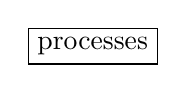
\begin{tikzpicture}
      \node [rectangle, text centered, draw=black]{processes};
    \end{tikzpicture},
    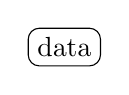
\begin{tikzpicture}
      \node [rectangle, rounded corners, text centered, draw=black]{data};
    \end{tikzpicture} and
    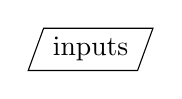
\begin{tikzpicture}
      \node [trapezium, trapezium left angle=70, trapezium right angle=110,
             text centered, draw=black]{inputs};
  \end{tikzpicture}}
  \label{fig:flow_chart}
\end{figure}

\section{Application}
\label{sec:application}

We have applied our benchmarking methodology to the \quickspec{} and \isacosy{}
MTE tools, using version 0.2 of the TIP (Tons of Inductive Problems) theorem
proving benchmark as our ground truth corpus~\cite{claessen2015tip}.

To determine our benchmarking parameters we ran some initial tests on both tools
for a few samples sized between 1 and 100, for an hour each on our benchmarking
machine with a 3.2GHz dual-core Intel i5 processor with hyper-threading and 8GB
of RAM. Most \quickspec{} runs either finished within 200 seconds or not at all,
and sizes above 20 mostly timed out. \isacosy{} mostly finished within 300 seconds
on sample sizes up to 4, but by size 8 was mostly timing out; its few successes
above this took thousands of seconds each, which we deemed infeasibly long.

Based on this we decided to benchmark sample sizes up to 20, since neither tool
seemed to perform well beyond that. The Speedup-Test protocol follows the
statistical ``rule of thumb'' of treating sample sizes $\leq$ 30 as ``small'',
so we pick 31 samples of each size in order to cross this threshold. This gave a
total of 1240 runs. To keep the benchmarking time down to a few days we chose a
timeout of 300 seconds, since that covered most of the successful \quickspec{} and
\isacosy{} results we saw, and longer times gave rapidly diminishing
returns. During analysis, duplicate samples (caused by our requirement that
samples have a non-empty ground truth) were found and discarded, so only 14
samples of size 1 were used and 30 of size 2.

\subsection{Tons of Inductive Problems}
\label{sec:tip}

We chose the Tons of Inductive Problems (TIP) benchmark for our ground truth
since it satisfies the criteria specified in $\S$\ref{section:prep}: each
benchmark problem has standalone type and function definitions, making their
separation trivial; known examples from the software verification and inductive
theorem proving literature are included, ensuring relevance to those fields; the
format includes the higher-order functions and inductive datatypes we are
interested in; it is large enough to pose a challenge to current MTE tools; plus
it is accompanied by tooling to convert its custom format (an extension of
SMT-Lib~\cite{BarFT-SMTLIB}) into a variety of languages, including Haskell and
Isabelle.

We use TIP version 0.2 which contains 343 problems, each stating a single
property and together defining a total of 618 datatypes and 1498 functions. Most
of these are duplicates, since each problem (re\nobreakdash-)defines all of the
datatypes and functions it involves.

TIP datatypes can have several ``constructors'' (introduction forms) and
``destructors'' (elimination forms; field accessors). For example the type of
lists from Figure~\ref{fig:list_theory} can be defined in the TIP format as
follows:

\begin{samepage}
\begin{verbatim}
(declare-datatypes
  (a)                       ;; Type parameter (element type)
  ((List                    ;; Type name
     (Nil)                  ;; Constructor (nullary)
     (Cons                  ;; Constructor (binary)
       (head a)             ;; Field name and type
       (tail (List a))))))  ;; Field name and type
\end{verbatim}
\end{samepage}

Our target languages (Haskell and Isabelle) differ in the way they handle
constructors and destructors, which complicates comparisons. To avoid this, we
generate a new function for each constructor (via $\eta$-expansion) and
destructor (via pattern-matching) of the following form:

\begin{samepage}
\begin{verbatim}
(define-fun
  (par (a)                   ;; Type parameter
    (constructor-Cons        ;; Function name
      ((x a) (xs (List a)))  ;; Argument names and types
      (List a)               ;; Return type
      (as                    ;; Type annotation
        (Cons x xs)          ;; Return value
        (List a)))))         ;; Return type
\end{verbatim}
\end{samepage}

\begin{samepage}
\begin{verbatim}
(define-fun
  (par (a)                        ;; Type parameter
    (destructor-head              ;; Function name
      ((xs (List a)))             ;; Argument name and type
      a                           ;; Return type
      (match xs                   ;; Pattern-match
        (case (Cons h t) h)))))   ;; Return relevant field
\end{verbatim}
\end{samepage}

\begin{sloppypar}
  We rewrite the TIP properties (our ground truth) to reference these expanded
  forms instead of the raw constructors and destructors, and use these functions
  in our samples in lieu of the raw expressions. Note that these destructor
  wrappers are \emph{partial} functions (e.g. \texttt{destructor-head} and
  \texttt{destructor-tail} are undefined for the input \texttt{Nil}), which
  complicates their translation to proof assistants like Isabelle.
\end{sloppypar}

Another complication is TIP's ``native'' support for booleans and integers,
which allows numerals and symbols like \texttt{+} to appear without any
accompanying definition. To ensure consistency in the translations, we replace
all occurrences of such expressions with standard definitions written with the
``user-level'' \texttt{declare-datatypes} and \texttt{define-fun}
mechanisms.~\footnote{\texttt{Boolean} has \texttt{true} and \texttt{false}
  constructors; \texttt{Natural} has \texttt{zero} and \texttt{successor};
  \texttt{Integer} has unary \texttt{positive} and \texttt{negative}
  constructors taking \texttt{Natural}s, and a nullary \texttt{zero} for
  symmetry.}

When we add all of these generated types and functions to those in TIP, we get a
total of 3598 definitions. Removing $\alpha$-equivalent duplicates leaves 269,
and we choose to only sample from those 182 functions which are referenced by at
least one property (this removes ambiguity about which \emph{definitions} count
as interesting and which are just ``implementation details'' for other
definitions).

TIP comes with software to translate its definitions into Haskell and Isabelle
code, including comparison functions and random data generators suitable for
\quickcheck{}. We translate all 269 unique definitions into a single module/theory
which is imported on each run of the tools, although only those functions which
appear in the current sample are included in the signature and explored. We also
encode all names in hexadecimal to avoid problems with language-specific naming
rules, for example \texttt{add} becomes \texttt{global616464} (the prefix
distinguishes these from local variables and prevents names from beginning with
a digit). This ensures that the generated conjectures will be using the same
names as the ground truth, rather than some language-specific variant.

\subsection{\quickspec{}}

We benchmarked \quickspec{} version 0.9.6, a tool written in Haskell for
conjecturing equations involving Haskell functions, described in more detail in
$\S$\ref{sec:theoryexploration}. In order to thoroughly benchmark \quickspec{},
we need to automate some of the decisions which are normally left up to the
user:

\begin{sloppypar}
  \begin{itemize}
  \item We must decide what variables to include. We choose to add three
    variables for each type that appears as a function argument, except for
    types which have no \quickcheck{} data generators.
  \item We must \emph{monomorphise} all types. For example, functions like
    \texttt{constructor-Cons} are \emph{polymorphic}: they build lists of any
    element type, but we need to pick a specific type in order to know which
    random value generator to use. We resolve this (arbitrarily) by picking
    \texttt{Integer}.~\footnote{We pick \texttt{Integer} for variables of kind
      \texttt{*} (types); for kind \texttt{* -> *} (type constructors) we pick
      \texttt{[]} (Haskell's list type constructor). If these violate some
      type class constraint, we pick a suitable type non-deterministically from
      those in scope during compilation; if no suitable type is found, we give
      up and don't include that function.}
  \item Haskell functions are ``black boxes'', which \quickspec{} can't compare
    during its exploration process. They are also curried, always taking one
    argument but potentially returning another function. \quickspec{} lets us
    assign an arity to each function in the signature, from 0 to 5, so we pick
    the highest that is type-correct, since this avoids a proliferation of
    incomparable, partially-applied functions.
  \end{itemize}
\end{sloppypar}

\begin{figure}
  \centering
  %% Creator: Matplotlib, PGF backend
%%
%% To include the figure in your LaTeX document, write
%%   \input{<filename>.pgf}
%%
%% Make sure the required packages are loaded in your preamble
%%   \usepackage{pgf}
%%
%% Figures using additional raster images can only be included by \input if
%% they are in the same directory as the main LaTeX file. For loading figures
%% from other directories you can use the `import` package
%%   \usepackage{import}
%% and then include the figures with
%%   \import{<path to file>}{<filename>.pgf}
%%
%% Matplotlib used the following preamble
%%   \usepackage[utf8x]{inputenc}
%%   \usepackage[T1]{fontenc}
%%
\begingroup%
\makeatletter%
\begin{pgfpicture}%
\pgfpathrectangle{\pgfpointorigin}{\pgfqpoint{3.202355in}{1.216845in}}%
\pgfusepath{use as bounding box, clip}%
\begin{pgfscope}%
\pgfsetbuttcap%
\pgfsetmiterjoin%
\definecolor{currentfill}{rgb}{1.000000,1.000000,1.000000}%
\pgfsetfillcolor{currentfill}%
\pgfsetlinewidth{0.000000pt}%
\definecolor{currentstroke}{rgb}{1.000000,1.000000,1.000000}%
\pgfsetstrokecolor{currentstroke}%
\pgfsetdash{}{0pt}%
\pgfpathmoveto{\pgfqpoint{-0.000000in}{0.000000in}}%
\pgfpathlineto{\pgfqpoint{3.202355in}{0.000000in}}%
\pgfpathlineto{\pgfqpoint{3.202355in}{1.216845in}}%
\pgfpathlineto{\pgfqpoint{-0.000000in}{1.216845in}}%
\pgfpathclose%
\pgfusepath{fill}%
\end{pgfscope}%
\begin{pgfscope}%
\pgfsetbuttcap%
\pgfsetmiterjoin%
\definecolor{currentfill}{rgb}{1.000000,1.000000,1.000000}%
\pgfsetfillcolor{currentfill}%
\pgfsetlinewidth{0.000000pt}%
\definecolor{currentstroke}{rgb}{0.000000,0.000000,0.000000}%
\pgfsetstrokecolor{currentstroke}%
\pgfsetstrokeopacity{0.000000}%
\pgfsetdash{}{0pt}%
\pgfpathmoveto{\pgfqpoint{0.448843in}{0.362833in}}%
\pgfpathlineto{\pgfqpoint{3.202355in}{0.362833in}}%
\pgfpathlineto{\pgfqpoint{3.202355in}{1.066550in}}%
\pgfpathlineto{\pgfqpoint{0.448843in}{1.066550in}}%
\pgfpathclose%
\pgfusepath{fill}%
\end{pgfscope}%
\begin{pgfscope}%
\pgfsetbuttcap%
\pgfsetroundjoin%
\definecolor{currentfill}{rgb}{0.150000,0.150000,0.150000}%
\pgfsetfillcolor{currentfill}%
\pgfsetlinewidth{0.803000pt}%
\definecolor{currentstroke}{rgb}{0.150000,0.150000,0.150000}%
\pgfsetstrokecolor{currentstroke}%
\pgfsetdash{}{0pt}%
\pgfsys@defobject{currentmarker}{\pgfqpoint{0.000000in}{0.000000in}}{\pgfqpoint{0.000000in}{0.000000in}}{%
\pgfpathmoveto{\pgfqpoint{0.000000in}{0.000000in}}%
\pgfpathlineto{\pgfqpoint{0.000000in}{0.000000in}}%
\pgfusepath{stroke,fill}%
}%
\begin{pgfscope}%
\pgfsys@transformshift{0.517681in}{0.362833in}%
\pgfsys@useobject{currentmarker}{}%
\end{pgfscope}%
\end{pgfscope}%
\begin{pgfscope}%
\pgfsetbuttcap%
\pgfsetroundjoin%
\definecolor{currentfill}{rgb}{0.150000,0.150000,0.150000}%
\pgfsetfillcolor{currentfill}%
\pgfsetlinewidth{0.803000pt}%
\definecolor{currentstroke}{rgb}{0.150000,0.150000,0.150000}%
\pgfsetstrokecolor{currentstroke}%
\pgfsetdash{}{0pt}%
\pgfsys@defobject{currentmarker}{\pgfqpoint{0.000000in}{0.000000in}}{\pgfqpoint{0.000000in}{0.000000in}}{%
\pgfpathmoveto{\pgfqpoint{0.000000in}{0.000000in}}%
\pgfpathlineto{\pgfqpoint{0.000000in}{0.000000in}}%
\pgfusepath{stroke,fill}%
}%
\begin{pgfscope}%
\pgfsys@transformshift{0.517681in}{1.066550in}%
\pgfsys@useobject{currentmarker}{}%
\end{pgfscope}%
\end{pgfscope}%
\begin{pgfscope}%
\definecolor{textcolor}{rgb}{0.150000,0.150000,0.150000}%
\pgfsetstrokecolor{textcolor}%
\pgfsetfillcolor{textcolor}%
\pgftext[x=0.517681in,y=0.285055in,,top]{\color{textcolor}\sffamily\fontsize{8.000000}{9.600000}\selectfont 1}%
\end{pgfscope}%
\begin{pgfscope}%
\pgfsetbuttcap%
\pgfsetroundjoin%
\definecolor{currentfill}{rgb}{0.150000,0.150000,0.150000}%
\pgfsetfillcolor{currentfill}%
\pgfsetlinewidth{0.803000pt}%
\definecolor{currentstroke}{rgb}{0.150000,0.150000,0.150000}%
\pgfsetstrokecolor{currentstroke}%
\pgfsetdash{}{0pt}%
\pgfsys@defobject{currentmarker}{\pgfqpoint{0.000000in}{0.000000in}}{\pgfqpoint{0.000000in}{0.000000in}}{%
\pgfpathmoveto{\pgfqpoint{0.000000in}{0.000000in}}%
\pgfpathlineto{\pgfqpoint{0.000000in}{0.000000in}}%
\pgfusepath{stroke,fill}%
}%
\begin{pgfscope}%
\pgfsys@transformshift{0.655357in}{0.362833in}%
\pgfsys@useobject{currentmarker}{}%
\end{pgfscope}%
\end{pgfscope}%
\begin{pgfscope}%
\pgfsetbuttcap%
\pgfsetroundjoin%
\definecolor{currentfill}{rgb}{0.150000,0.150000,0.150000}%
\pgfsetfillcolor{currentfill}%
\pgfsetlinewidth{0.803000pt}%
\definecolor{currentstroke}{rgb}{0.150000,0.150000,0.150000}%
\pgfsetstrokecolor{currentstroke}%
\pgfsetdash{}{0pt}%
\pgfsys@defobject{currentmarker}{\pgfqpoint{0.000000in}{0.000000in}}{\pgfqpoint{0.000000in}{0.000000in}}{%
\pgfpathmoveto{\pgfqpoint{0.000000in}{0.000000in}}%
\pgfpathlineto{\pgfqpoint{0.000000in}{0.000000in}}%
\pgfusepath{stroke,fill}%
}%
\begin{pgfscope}%
\pgfsys@transformshift{0.655357in}{1.066550in}%
\pgfsys@useobject{currentmarker}{}%
\end{pgfscope}%
\end{pgfscope}%
\begin{pgfscope}%
\definecolor{textcolor}{rgb}{0.150000,0.150000,0.150000}%
\pgfsetstrokecolor{textcolor}%
\pgfsetfillcolor{textcolor}%
\pgftext[x=0.655357in,y=0.285055in,,top]{\color{textcolor}\sffamily\fontsize{8.000000}{9.600000}\selectfont 2}%
\end{pgfscope}%
\begin{pgfscope}%
\pgfsetbuttcap%
\pgfsetroundjoin%
\definecolor{currentfill}{rgb}{0.150000,0.150000,0.150000}%
\pgfsetfillcolor{currentfill}%
\pgfsetlinewidth{0.803000pt}%
\definecolor{currentstroke}{rgb}{0.150000,0.150000,0.150000}%
\pgfsetstrokecolor{currentstroke}%
\pgfsetdash{}{0pt}%
\pgfsys@defobject{currentmarker}{\pgfqpoint{0.000000in}{0.000000in}}{\pgfqpoint{0.000000in}{0.000000in}}{%
\pgfpathmoveto{\pgfqpoint{0.000000in}{0.000000in}}%
\pgfpathlineto{\pgfqpoint{0.000000in}{0.000000in}}%
\pgfusepath{stroke,fill}%
}%
\begin{pgfscope}%
\pgfsys@transformshift{0.793032in}{0.362833in}%
\pgfsys@useobject{currentmarker}{}%
\end{pgfscope}%
\end{pgfscope}%
\begin{pgfscope}%
\pgfsetbuttcap%
\pgfsetroundjoin%
\definecolor{currentfill}{rgb}{0.150000,0.150000,0.150000}%
\pgfsetfillcolor{currentfill}%
\pgfsetlinewidth{0.803000pt}%
\definecolor{currentstroke}{rgb}{0.150000,0.150000,0.150000}%
\pgfsetstrokecolor{currentstroke}%
\pgfsetdash{}{0pt}%
\pgfsys@defobject{currentmarker}{\pgfqpoint{0.000000in}{0.000000in}}{\pgfqpoint{0.000000in}{0.000000in}}{%
\pgfpathmoveto{\pgfqpoint{0.000000in}{0.000000in}}%
\pgfpathlineto{\pgfqpoint{0.000000in}{0.000000in}}%
\pgfusepath{stroke,fill}%
}%
\begin{pgfscope}%
\pgfsys@transformshift{0.793032in}{1.066550in}%
\pgfsys@useobject{currentmarker}{}%
\end{pgfscope}%
\end{pgfscope}%
\begin{pgfscope}%
\definecolor{textcolor}{rgb}{0.150000,0.150000,0.150000}%
\pgfsetstrokecolor{textcolor}%
\pgfsetfillcolor{textcolor}%
\pgftext[x=0.793032in,y=0.285055in,,top]{\color{textcolor}\sffamily\fontsize{8.000000}{9.600000}\selectfont 3}%
\end{pgfscope}%
\begin{pgfscope}%
\pgfsetbuttcap%
\pgfsetroundjoin%
\definecolor{currentfill}{rgb}{0.150000,0.150000,0.150000}%
\pgfsetfillcolor{currentfill}%
\pgfsetlinewidth{0.803000pt}%
\definecolor{currentstroke}{rgb}{0.150000,0.150000,0.150000}%
\pgfsetstrokecolor{currentstroke}%
\pgfsetdash{}{0pt}%
\pgfsys@defobject{currentmarker}{\pgfqpoint{0.000000in}{0.000000in}}{\pgfqpoint{0.000000in}{0.000000in}}{%
\pgfpathmoveto{\pgfqpoint{0.000000in}{0.000000in}}%
\pgfpathlineto{\pgfqpoint{0.000000in}{0.000000in}}%
\pgfusepath{stroke,fill}%
}%
\begin{pgfscope}%
\pgfsys@transformshift{0.930708in}{0.362833in}%
\pgfsys@useobject{currentmarker}{}%
\end{pgfscope}%
\end{pgfscope}%
\begin{pgfscope}%
\pgfsetbuttcap%
\pgfsetroundjoin%
\definecolor{currentfill}{rgb}{0.150000,0.150000,0.150000}%
\pgfsetfillcolor{currentfill}%
\pgfsetlinewidth{0.803000pt}%
\definecolor{currentstroke}{rgb}{0.150000,0.150000,0.150000}%
\pgfsetstrokecolor{currentstroke}%
\pgfsetdash{}{0pt}%
\pgfsys@defobject{currentmarker}{\pgfqpoint{0.000000in}{0.000000in}}{\pgfqpoint{0.000000in}{0.000000in}}{%
\pgfpathmoveto{\pgfqpoint{0.000000in}{0.000000in}}%
\pgfpathlineto{\pgfqpoint{0.000000in}{0.000000in}}%
\pgfusepath{stroke,fill}%
}%
\begin{pgfscope}%
\pgfsys@transformshift{0.930708in}{1.066550in}%
\pgfsys@useobject{currentmarker}{}%
\end{pgfscope}%
\end{pgfscope}%
\begin{pgfscope}%
\definecolor{textcolor}{rgb}{0.150000,0.150000,0.150000}%
\pgfsetstrokecolor{textcolor}%
\pgfsetfillcolor{textcolor}%
\pgftext[x=0.930708in,y=0.285055in,,top]{\color{textcolor}\sffamily\fontsize{8.000000}{9.600000}\selectfont 4}%
\end{pgfscope}%
\begin{pgfscope}%
\pgfsetbuttcap%
\pgfsetroundjoin%
\definecolor{currentfill}{rgb}{0.150000,0.150000,0.150000}%
\pgfsetfillcolor{currentfill}%
\pgfsetlinewidth{0.803000pt}%
\definecolor{currentstroke}{rgb}{0.150000,0.150000,0.150000}%
\pgfsetstrokecolor{currentstroke}%
\pgfsetdash{}{0pt}%
\pgfsys@defobject{currentmarker}{\pgfqpoint{0.000000in}{0.000000in}}{\pgfqpoint{0.000000in}{0.000000in}}{%
\pgfpathmoveto{\pgfqpoint{0.000000in}{0.000000in}}%
\pgfpathlineto{\pgfqpoint{0.000000in}{0.000000in}}%
\pgfusepath{stroke,fill}%
}%
\begin{pgfscope}%
\pgfsys@transformshift{1.068384in}{0.362833in}%
\pgfsys@useobject{currentmarker}{}%
\end{pgfscope}%
\end{pgfscope}%
\begin{pgfscope}%
\pgfsetbuttcap%
\pgfsetroundjoin%
\definecolor{currentfill}{rgb}{0.150000,0.150000,0.150000}%
\pgfsetfillcolor{currentfill}%
\pgfsetlinewidth{0.803000pt}%
\definecolor{currentstroke}{rgb}{0.150000,0.150000,0.150000}%
\pgfsetstrokecolor{currentstroke}%
\pgfsetdash{}{0pt}%
\pgfsys@defobject{currentmarker}{\pgfqpoint{0.000000in}{0.000000in}}{\pgfqpoint{0.000000in}{0.000000in}}{%
\pgfpathmoveto{\pgfqpoint{0.000000in}{0.000000in}}%
\pgfpathlineto{\pgfqpoint{0.000000in}{0.000000in}}%
\pgfusepath{stroke,fill}%
}%
\begin{pgfscope}%
\pgfsys@transformshift{1.068384in}{1.066550in}%
\pgfsys@useobject{currentmarker}{}%
\end{pgfscope}%
\end{pgfscope}%
\begin{pgfscope}%
\definecolor{textcolor}{rgb}{0.150000,0.150000,0.150000}%
\pgfsetstrokecolor{textcolor}%
\pgfsetfillcolor{textcolor}%
\pgftext[x=1.068384in,y=0.285055in,,top]{\color{textcolor}\sffamily\fontsize{8.000000}{9.600000}\selectfont 5}%
\end{pgfscope}%
\begin{pgfscope}%
\pgfsetbuttcap%
\pgfsetroundjoin%
\definecolor{currentfill}{rgb}{0.150000,0.150000,0.150000}%
\pgfsetfillcolor{currentfill}%
\pgfsetlinewidth{0.803000pt}%
\definecolor{currentstroke}{rgb}{0.150000,0.150000,0.150000}%
\pgfsetstrokecolor{currentstroke}%
\pgfsetdash{}{0pt}%
\pgfsys@defobject{currentmarker}{\pgfqpoint{0.000000in}{0.000000in}}{\pgfqpoint{0.000000in}{0.000000in}}{%
\pgfpathmoveto{\pgfqpoint{0.000000in}{0.000000in}}%
\pgfpathlineto{\pgfqpoint{0.000000in}{0.000000in}}%
\pgfusepath{stroke,fill}%
}%
\begin{pgfscope}%
\pgfsys@transformshift{1.206059in}{0.362833in}%
\pgfsys@useobject{currentmarker}{}%
\end{pgfscope}%
\end{pgfscope}%
\begin{pgfscope}%
\pgfsetbuttcap%
\pgfsetroundjoin%
\definecolor{currentfill}{rgb}{0.150000,0.150000,0.150000}%
\pgfsetfillcolor{currentfill}%
\pgfsetlinewidth{0.803000pt}%
\definecolor{currentstroke}{rgb}{0.150000,0.150000,0.150000}%
\pgfsetstrokecolor{currentstroke}%
\pgfsetdash{}{0pt}%
\pgfsys@defobject{currentmarker}{\pgfqpoint{0.000000in}{0.000000in}}{\pgfqpoint{0.000000in}{0.000000in}}{%
\pgfpathmoveto{\pgfqpoint{0.000000in}{0.000000in}}%
\pgfpathlineto{\pgfqpoint{0.000000in}{0.000000in}}%
\pgfusepath{stroke,fill}%
}%
\begin{pgfscope}%
\pgfsys@transformshift{1.206059in}{1.066550in}%
\pgfsys@useobject{currentmarker}{}%
\end{pgfscope}%
\end{pgfscope}%
\begin{pgfscope}%
\definecolor{textcolor}{rgb}{0.150000,0.150000,0.150000}%
\pgfsetstrokecolor{textcolor}%
\pgfsetfillcolor{textcolor}%
\pgftext[x=1.206059in,y=0.285055in,,top]{\color{textcolor}\sffamily\fontsize{8.000000}{9.600000}\selectfont 6}%
\end{pgfscope}%
\begin{pgfscope}%
\pgfsetbuttcap%
\pgfsetroundjoin%
\definecolor{currentfill}{rgb}{0.150000,0.150000,0.150000}%
\pgfsetfillcolor{currentfill}%
\pgfsetlinewidth{0.803000pt}%
\definecolor{currentstroke}{rgb}{0.150000,0.150000,0.150000}%
\pgfsetstrokecolor{currentstroke}%
\pgfsetdash{}{0pt}%
\pgfsys@defobject{currentmarker}{\pgfqpoint{0.000000in}{0.000000in}}{\pgfqpoint{0.000000in}{0.000000in}}{%
\pgfpathmoveto{\pgfqpoint{0.000000in}{0.000000in}}%
\pgfpathlineto{\pgfqpoint{0.000000in}{0.000000in}}%
\pgfusepath{stroke,fill}%
}%
\begin{pgfscope}%
\pgfsys@transformshift{1.343735in}{0.362833in}%
\pgfsys@useobject{currentmarker}{}%
\end{pgfscope}%
\end{pgfscope}%
\begin{pgfscope}%
\pgfsetbuttcap%
\pgfsetroundjoin%
\definecolor{currentfill}{rgb}{0.150000,0.150000,0.150000}%
\pgfsetfillcolor{currentfill}%
\pgfsetlinewidth{0.803000pt}%
\definecolor{currentstroke}{rgb}{0.150000,0.150000,0.150000}%
\pgfsetstrokecolor{currentstroke}%
\pgfsetdash{}{0pt}%
\pgfsys@defobject{currentmarker}{\pgfqpoint{0.000000in}{0.000000in}}{\pgfqpoint{0.000000in}{0.000000in}}{%
\pgfpathmoveto{\pgfqpoint{0.000000in}{0.000000in}}%
\pgfpathlineto{\pgfqpoint{0.000000in}{0.000000in}}%
\pgfusepath{stroke,fill}%
}%
\begin{pgfscope}%
\pgfsys@transformshift{1.343735in}{1.066550in}%
\pgfsys@useobject{currentmarker}{}%
\end{pgfscope}%
\end{pgfscope}%
\begin{pgfscope}%
\definecolor{textcolor}{rgb}{0.150000,0.150000,0.150000}%
\pgfsetstrokecolor{textcolor}%
\pgfsetfillcolor{textcolor}%
\pgftext[x=1.343735in,y=0.285055in,,top]{\color{textcolor}\sffamily\fontsize{8.000000}{9.600000}\selectfont 7}%
\end{pgfscope}%
\begin{pgfscope}%
\pgfsetbuttcap%
\pgfsetroundjoin%
\definecolor{currentfill}{rgb}{0.150000,0.150000,0.150000}%
\pgfsetfillcolor{currentfill}%
\pgfsetlinewidth{0.803000pt}%
\definecolor{currentstroke}{rgb}{0.150000,0.150000,0.150000}%
\pgfsetstrokecolor{currentstroke}%
\pgfsetdash{}{0pt}%
\pgfsys@defobject{currentmarker}{\pgfqpoint{0.000000in}{0.000000in}}{\pgfqpoint{0.000000in}{0.000000in}}{%
\pgfpathmoveto{\pgfqpoint{0.000000in}{0.000000in}}%
\pgfpathlineto{\pgfqpoint{0.000000in}{0.000000in}}%
\pgfusepath{stroke,fill}%
}%
\begin{pgfscope}%
\pgfsys@transformshift{1.481410in}{0.362833in}%
\pgfsys@useobject{currentmarker}{}%
\end{pgfscope}%
\end{pgfscope}%
\begin{pgfscope}%
\pgfsetbuttcap%
\pgfsetroundjoin%
\definecolor{currentfill}{rgb}{0.150000,0.150000,0.150000}%
\pgfsetfillcolor{currentfill}%
\pgfsetlinewidth{0.803000pt}%
\definecolor{currentstroke}{rgb}{0.150000,0.150000,0.150000}%
\pgfsetstrokecolor{currentstroke}%
\pgfsetdash{}{0pt}%
\pgfsys@defobject{currentmarker}{\pgfqpoint{0.000000in}{0.000000in}}{\pgfqpoint{0.000000in}{0.000000in}}{%
\pgfpathmoveto{\pgfqpoint{0.000000in}{0.000000in}}%
\pgfpathlineto{\pgfqpoint{0.000000in}{0.000000in}}%
\pgfusepath{stroke,fill}%
}%
\begin{pgfscope}%
\pgfsys@transformshift{1.481410in}{1.066550in}%
\pgfsys@useobject{currentmarker}{}%
\end{pgfscope}%
\end{pgfscope}%
\begin{pgfscope}%
\definecolor{textcolor}{rgb}{0.150000,0.150000,0.150000}%
\pgfsetstrokecolor{textcolor}%
\pgfsetfillcolor{textcolor}%
\pgftext[x=1.481410in,y=0.285055in,,top]{\color{textcolor}\sffamily\fontsize{8.000000}{9.600000}\selectfont 8}%
\end{pgfscope}%
\begin{pgfscope}%
\pgfsetbuttcap%
\pgfsetroundjoin%
\definecolor{currentfill}{rgb}{0.150000,0.150000,0.150000}%
\pgfsetfillcolor{currentfill}%
\pgfsetlinewidth{0.803000pt}%
\definecolor{currentstroke}{rgb}{0.150000,0.150000,0.150000}%
\pgfsetstrokecolor{currentstroke}%
\pgfsetdash{}{0pt}%
\pgfsys@defobject{currentmarker}{\pgfqpoint{0.000000in}{0.000000in}}{\pgfqpoint{0.000000in}{0.000000in}}{%
\pgfpathmoveto{\pgfqpoint{0.000000in}{0.000000in}}%
\pgfpathlineto{\pgfqpoint{0.000000in}{0.000000in}}%
\pgfusepath{stroke,fill}%
}%
\begin{pgfscope}%
\pgfsys@transformshift{1.619086in}{0.362833in}%
\pgfsys@useobject{currentmarker}{}%
\end{pgfscope}%
\end{pgfscope}%
\begin{pgfscope}%
\pgfsetbuttcap%
\pgfsetroundjoin%
\definecolor{currentfill}{rgb}{0.150000,0.150000,0.150000}%
\pgfsetfillcolor{currentfill}%
\pgfsetlinewidth{0.803000pt}%
\definecolor{currentstroke}{rgb}{0.150000,0.150000,0.150000}%
\pgfsetstrokecolor{currentstroke}%
\pgfsetdash{}{0pt}%
\pgfsys@defobject{currentmarker}{\pgfqpoint{0.000000in}{0.000000in}}{\pgfqpoint{0.000000in}{0.000000in}}{%
\pgfpathmoveto{\pgfqpoint{0.000000in}{0.000000in}}%
\pgfpathlineto{\pgfqpoint{0.000000in}{0.000000in}}%
\pgfusepath{stroke,fill}%
}%
\begin{pgfscope}%
\pgfsys@transformshift{1.619086in}{1.066550in}%
\pgfsys@useobject{currentmarker}{}%
\end{pgfscope}%
\end{pgfscope}%
\begin{pgfscope}%
\definecolor{textcolor}{rgb}{0.150000,0.150000,0.150000}%
\pgfsetstrokecolor{textcolor}%
\pgfsetfillcolor{textcolor}%
\pgftext[x=1.619086in,y=0.285055in,,top]{\color{textcolor}\sffamily\fontsize{8.000000}{9.600000}\selectfont 9}%
\end{pgfscope}%
\begin{pgfscope}%
\pgfsetbuttcap%
\pgfsetroundjoin%
\definecolor{currentfill}{rgb}{0.150000,0.150000,0.150000}%
\pgfsetfillcolor{currentfill}%
\pgfsetlinewidth{0.803000pt}%
\definecolor{currentstroke}{rgb}{0.150000,0.150000,0.150000}%
\pgfsetstrokecolor{currentstroke}%
\pgfsetdash{}{0pt}%
\pgfsys@defobject{currentmarker}{\pgfqpoint{0.000000in}{0.000000in}}{\pgfqpoint{0.000000in}{0.000000in}}{%
\pgfpathmoveto{\pgfqpoint{0.000000in}{0.000000in}}%
\pgfpathlineto{\pgfqpoint{0.000000in}{0.000000in}}%
\pgfusepath{stroke,fill}%
}%
\begin{pgfscope}%
\pgfsys@transformshift{1.756762in}{0.362833in}%
\pgfsys@useobject{currentmarker}{}%
\end{pgfscope}%
\end{pgfscope}%
\begin{pgfscope}%
\pgfsetbuttcap%
\pgfsetroundjoin%
\definecolor{currentfill}{rgb}{0.150000,0.150000,0.150000}%
\pgfsetfillcolor{currentfill}%
\pgfsetlinewidth{0.803000pt}%
\definecolor{currentstroke}{rgb}{0.150000,0.150000,0.150000}%
\pgfsetstrokecolor{currentstroke}%
\pgfsetdash{}{0pt}%
\pgfsys@defobject{currentmarker}{\pgfqpoint{0.000000in}{0.000000in}}{\pgfqpoint{0.000000in}{0.000000in}}{%
\pgfpathmoveto{\pgfqpoint{0.000000in}{0.000000in}}%
\pgfpathlineto{\pgfqpoint{0.000000in}{0.000000in}}%
\pgfusepath{stroke,fill}%
}%
\begin{pgfscope}%
\pgfsys@transformshift{1.756762in}{1.066550in}%
\pgfsys@useobject{currentmarker}{}%
\end{pgfscope}%
\end{pgfscope}%
\begin{pgfscope}%
\definecolor{textcolor}{rgb}{0.150000,0.150000,0.150000}%
\pgfsetstrokecolor{textcolor}%
\pgfsetfillcolor{textcolor}%
\pgftext[x=1.756762in,y=0.285055in,,top]{\color{textcolor}\sffamily\fontsize{8.000000}{9.600000}\selectfont 10}%
\end{pgfscope}%
\begin{pgfscope}%
\pgfsetbuttcap%
\pgfsetroundjoin%
\definecolor{currentfill}{rgb}{0.150000,0.150000,0.150000}%
\pgfsetfillcolor{currentfill}%
\pgfsetlinewidth{0.803000pt}%
\definecolor{currentstroke}{rgb}{0.150000,0.150000,0.150000}%
\pgfsetstrokecolor{currentstroke}%
\pgfsetdash{}{0pt}%
\pgfsys@defobject{currentmarker}{\pgfqpoint{0.000000in}{0.000000in}}{\pgfqpoint{0.000000in}{0.000000in}}{%
\pgfpathmoveto{\pgfqpoint{0.000000in}{0.000000in}}%
\pgfpathlineto{\pgfqpoint{0.000000in}{0.000000in}}%
\pgfusepath{stroke,fill}%
}%
\begin{pgfscope}%
\pgfsys@transformshift{1.894437in}{0.362833in}%
\pgfsys@useobject{currentmarker}{}%
\end{pgfscope}%
\end{pgfscope}%
\begin{pgfscope}%
\pgfsetbuttcap%
\pgfsetroundjoin%
\definecolor{currentfill}{rgb}{0.150000,0.150000,0.150000}%
\pgfsetfillcolor{currentfill}%
\pgfsetlinewidth{0.803000pt}%
\definecolor{currentstroke}{rgb}{0.150000,0.150000,0.150000}%
\pgfsetstrokecolor{currentstroke}%
\pgfsetdash{}{0pt}%
\pgfsys@defobject{currentmarker}{\pgfqpoint{0.000000in}{0.000000in}}{\pgfqpoint{0.000000in}{0.000000in}}{%
\pgfpathmoveto{\pgfqpoint{0.000000in}{0.000000in}}%
\pgfpathlineto{\pgfqpoint{0.000000in}{0.000000in}}%
\pgfusepath{stroke,fill}%
}%
\begin{pgfscope}%
\pgfsys@transformshift{1.894437in}{1.066550in}%
\pgfsys@useobject{currentmarker}{}%
\end{pgfscope}%
\end{pgfscope}%
\begin{pgfscope}%
\definecolor{textcolor}{rgb}{0.150000,0.150000,0.150000}%
\pgfsetstrokecolor{textcolor}%
\pgfsetfillcolor{textcolor}%
\pgftext[x=1.894437in,y=0.285055in,,top]{\color{textcolor}\sffamily\fontsize{8.000000}{9.600000}\selectfont 11}%
\end{pgfscope}%
\begin{pgfscope}%
\pgfsetbuttcap%
\pgfsetroundjoin%
\definecolor{currentfill}{rgb}{0.150000,0.150000,0.150000}%
\pgfsetfillcolor{currentfill}%
\pgfsetlinewidth{0.803000pt}%
\definecolor{currentstroke}{rgb}{0.150000,0.150000,0.150000}%
\pgfsetstrokecolor{currentstroke}%
\pgfsetdash{}{0pt}%
\pgfsys@defobject{currentmarker}{\pgfqpoint{0.000000in}{0.000000in}}{\pgfqpoint{0.000000in}{0.000000in}}{%
\pgfpathmoveto{\pgfqpoint{0.000000in}{0.000000in}}%
\pgfpathlineto{\pgfqpoint{0.000000in}{0.000000in}}%
\pgfusepath{stroke,fill}%
}%
\begin{pgfscope}%
\pgfsys@transformshift{2.032113in}{0.362833in}%
\pgfsys@useobject{currentmarker}{}%
\end{pgfscope}%
\end{pgfscope}%
\begin{pgfscope}%
\pgfsetbuttcap%
\pgfsetroundjoin%
\definecolor{currentfill}{rgb}{0.150000,0.150000,0.150000}%
\pgfsetfillcolor{currentfill}%
\pgfsetlinewidth{0.803000pt}%
\definecolor{currentstroke}{rgb}{0.150000,0.150000,0.150000}%
\pgfsetstrokecolor{currentstroke}%
\pgfsetdash{}{0pt}%
\pgfsys@defobject{currentmarker}{\pgfqpoint{0.000000in}{0.000000in}}{\pgfqpoint{0.000000in}{0.000000in}}{%
\pgfpathmoveto{\pgfqpoint{0.000000in}{0.000000in}}%
\pgfpathlineto{\pgfqpoint{0.000000in}{0.000000in}}%
\pgfusepath{stroke,fill}%
}%
\begin{pgfscope}%
\pgfsys@transformshift{2.032113in}{1.066550in}%
\pgfsys@useobject{currentmarker}{}%
\end{pgfscope}%
\end{pgfscope}%
\begin{pgfscope}%
\definecolor{textcolor}{rgb}{0.150000,0.150000,0.150000}%
\pgfsetstrokecolor{textcolor}%
\pgfsetfillcolor{textcolor}%
\pgftext[x=2.032113in,y=0.285055in,,top]{\color{textcolor}\sffamily\fontsize{8.000000}{9.600000}\selectfont 12}%
\end{pgfscope}%
\begin{pgfscope}%
\pgfsetbuttcap%
\pgfsetroundjoin%
\definecolor{currentfill}{rgb}{0.150000,0.150000,0.150000}%
\pgfsetfillcolor{currentfill}%
\pgfsetlinewidth{0.803000pt}%
\definecolor{currentstroke}{rgb}{0.150000,0.150000,0.150000}%
\pgfsetstrokecolor{currentstroke}%
\pgfsetdash{}{0pt}%
\pgfsys@defobject{currentmarker}{\pgfqpoint{0.000000in}{0.000000in}}{\pgfqpoint{0.000000in}{0.000000in}}{%
\pgfpathmoveto{\pgfqpoint{0.000000in}{0.000000in}}%
\pgfpathlineto{\pgfqpoint{0.000000in}{0.000000in}}%
\pgfusepath{stroke,fill}%
}%
\begin{pgfscope}%
\pgfsys@transformshift{2.169788in}{0.362833in}%
\pgfsys@useobject{currentmarker}{}%
\end{pgfscope}%
\end{pgfscope}%
\begin{pgfscope}%
\pgfsetbuttcap%
\pgfsetroundjoin%
\definecolor{currentfill}{rgb}{0.150000,0.150000,0.150000}%
\pgfsetfillcolor{currentfill}%
\pgfsetlinewidth{0.803000pt}%
\definecolor{currentstroke}{rgb}{0.150000,0.150000,0.150000}%
\pgfsetstrokecolor{currentstroke}%
\pgfsetdash{}{0pt}%
\pgfsys@defobject{currentmarker}{\pgfqpoint{0.000000in}{0.000000in}}{\pgfqpoint{0.000000in}{0.000000in}}{%
\pgfpathmoveto{\pgfqpoint{0.000000in}{0.000000in}}%
\pgfpathlineto{\pgfqpoint{0.000000in}{0.000000in}}%
\pgfusepath{stroke,fill}%
}%
\begin{pgfscope}%
\pgfsys@transformshift{2.169788in}{1.066550in}%
\pgfsys@useobject{currentmarker}{}%
\end{pgfscope}%
\end{pgfscope}%
\begin{pgfscope}%
\definecolor{textcolor}{rgb}{0.150000,0.150000,0.150000}%
\pgfsetstrokecolor{textcolor}%
\pgfsetfillcolor{textcolor}%
\pgftext[x=2.169788in,y=0.285055in,,top]{\color{textcolor}\sffamily\fontsize{8.000000}{9.600000}\selectfont 13}%
\end{pgfscope}%
\begin{pgfscope}%
\pgfsetbuttcap%
\pgfsetroundjoin%
\definecolor{currentfill}{rgb}{0.150000,0.150000,0.150000}%
\pgfsetfillcolor{currentfill}%
\pgfsetlinewidth{0.803000pt}%
\definecolor{currentstroke}{rgb}{0.150000,0.150000,0.150000}%
\pgfsetstrokecolor{currentstroke}%
\pgfsetdash{}{0pt}%
\pgfsys@defobject{currentmarker}{\pgfqpoint{0.000000in}{0.000000in}}{\pgfqpoint{0.000000in}{0.000000in}}{%
\pgfpathmoveto{\pgfqpoint{0.000000in}{0.000000in}}%
\pgfpathlineto{\pgfqpoint{0.000000in}{0.000000in}}%
\pgfusepath{stroke,fill}%
}%
\begin{pgfscope}%
\pgfsys@transformshift{2.307464in}{0.362833in}%
\pgfsys@useobject{currentmarker}{}%
\end{pgfscope}%
\end{pgfscope}%
\begin{pgfscope}%
\pgfsetbuttcap%
\pgfsetroundjoin%
\definecolor{currentfill}{rgb}{0.150000,0.150000,0.150000}%
\pgfsetfillcolor{currentfill}%
\pgfsetlinewidth{0.803000pt}%
\definecolor{currentstroke}{rgb}{0.150000,0.150000,0.150000}%
\pgfsetstrokecolor{currentstroke}%
\pgfsetdash{}{0pt}%
\pgfsys@defobject{currentmarker}{\pgfqpoint{0.000000in}{0.000000in}}{\pgfqpoint{0.000000in}{0.000000in}}{%
\pgfpathmoveto{\pgfqpoint{0.000000in}{0.000000in}}%
\pgfpathlineto{\pgfqpoint{0.000000in}{0.000000in}}%
\pgfusepath{stroke,fill}%
}%
\begin{pgfscope}%
\pgfsys@transformshift{2.307464in}{1.066550in}%
\pgfsys@useobject{currentmarker}{}%
\end{pgfscope}%
\end{pgfscope}%
\begin{pgfscope}%
\definecolor{textcolor}{rgb}{0.150000,0.150000,0.150000}%
\pgfsetstrokecolor{textcolor}%
\pgfsetfillcolor{textcolor}%
\pgftext[x=2.307464in,y=0.285055in,,top]{\color{textcolor}\sffamily\fontsize{8.000000}{9.600000}\selectfont 14}%
\end{pgfscope}%
\begin{pgfscope}%
\pgfsetbuttcap%
\pgfsetroundjoin%
\definecolor{currentfill}{rgb}{0.150000,0.150000,0.150000}%
\pgfsetfillcolor{currentfill}%
\pgfsetlinewidth{0.803000pt}%
\definecolor{currentstroke}{rgb}{0.150000,0.150000,0.150000}%
\pgfsetstrokecolor{currentstroke}%
\pgfsetdash{}{0pt}%
\pgfsys@defobject{currentmarker}{\pgfqpoint{0.000000in}{0.000000in}}{\pgfqpoint{0.000000in}{0.000000in}}{%
\pgfpathmoveto{\pgfqpoint{0.000000in}{0.000000in}}%
\pgfpathlineto{\pgfqpoint{0.000000in}{0.000000in}}%
\pgfusepath{stroke,fill}%
}%
\begin{pgfscope}%
\pgfsys@transformshift{2.445140in}{0.362833in}%
\pgfsys@useobject{currentmarker}{}%
\end{pgfscope}%
\end{pgfscope}%
\begin{pgfscope}%
\pgfsetbuttcap%
\pgfsetroundjoin%
\definecolor{currentfill}{rgb}{0.150000,0.150000,0.150000}%
\pgfsetfillcolor{currentfill}%
\pgfsetlinewidth{0.803000pt}%
\definecolor{currentstroke}{rgb}{0.150000,0.150000,0.150000}%
\pgfsetstrokecolor{currentstroke}%
\pgfsetdash{}{0pt}%
\pgfsys@defobject{currentmarker}{\pgfqpoint{0.000000in}{0.000000in}}{\pgfqpoint{0.000000in}{0.000000in}}{%
\pgfpathmoveto{\pgfqpoint{0.000000in}{0.000000in}}%
\pgfpathlineto{\pgfqpoint{0.000000in}{0.000000in}}%
\pgfusepath{stroke,fill}%
}%
\begin{pgfscope}%
\pgfsys@transformshift{2.445140in}{1.066550in}%
\pgfsys@useobject{currentmarker}{}%
\end{pgfscope}%
\end{pgfscope}%
\begin{pgfscope}%
\definecolor{textcolor}{rgb}{0.150000,0.150000,0.150000}%
\pgfsetstrokecolor{textcolor}%
\pgfsetfillcolor{textcolor}%
\pgftext[x=2.445140in,y=0.285055in,,top]{\color{textcolor}\sffamily\fontsize{8.000000}{9.600000}\selectfont 15}%
\end{pgfscope}%
\begin{pgfscope}%
\pgfsetbuttcap%
\pgfsetroundjoin%
\definecolor{currentfill}{rgb}{0.150000,0.150000,0.150000}%
\pgfsetfillcolor{currentfill}%
\pgfsetlinewidth{0.803000pt}%
\definecolor{currentstroke}{rgb}{0.150000,0.150000,0.150000}%
\pgfsetstrokecolor{currentstroke}%
\pgfsetdash{}{0pt}%
\pgfsys@defobject{currentmarker}{\pgfqpoint{0.000000in}{0.000000in}}{\pgfqpoint{0.000000in}{0.000000in}}{%
\pgfpathmoveto{\pgfqpoint{0.000000in}{0.000000in}}%
\pgfpathlineto{\pgfqpoint{0.000000in}{0.000000in}}%
\pgfusepath{stroke,fill}%
}%
\begin{pgfscope}%
\pgfsys@transformshift{2.582815in}{0.362833in}%
\pgfsys@useobject{currentmarker}{}%
\end{pgfscope}%
\end{pgfscope}%
\begin{pgfscope}%
\pgfsetbuttcap%
\pgfsetroundjoin%
\definecolor{currentfill}{rgb}{0.150000,0.150000,0.150000}%
\pgfsetfillcolor{currentfill}%
\pgfsetlinewidth{0.803000pt}%
\definecolor{currentstroke}{rgb}{0.150000,0.150000,0.150000}%
\pgfsetstrokecolor{currentstroke}%
\pgfsetdash{}{0pt}%
\pgfsys@defobject{currentmarker}{\pgfqpoint{0.000000in}{0.000000in}}{\pgfqpoint{0.000000in}{0.000000in}}{%
\pgfpathmoveto{\pgfqpoint{0.000000in}{0.000000in}}%
\pgfpathlineto{\pgfqpoint{0.000000in}{0.000000in}}%
\pgfusepath{stroke,fill}%
}%
\begin{pgfscope}%
\pgfsys@transformshift{2.582815in}{1.066550in}%
\pgfsys@useobject{currentmarker}{}%
\end{pgfscope}%
\end{pgfscope}%
\begin{pgfscope}%
\definecolor{textcolor}{rgb}{0.150000,0.150000,0.150000}%
\pgfsetstrokecolor{textcolor}%
\pgfsetfillcolor{textcolor}%
\pgftext[x=2.582815in,y=0.285055in,,top]{\color{textcolor}\sffamily\fontsize{8.000000}{9.600000}\selectfont 16}%
\end{pgfscope}%
\begin{pgfscope}%
\pgfsetbuttcap%
\pgfsetroundjoin%
\definecolor{currentfill}{rgb}{0.150000,0.150000,0.150000}%
\pgfsetfillcolor{currentfill}%
\pgfsetlinewidth{0.803000pt}%
\definecolor{currentstroke}{rgb}{0.150000,0.150000,0.150000}%
\pgfsetstrokecolor{currentstroke}%
\pgfsetdash{}{0pt}%
\pgfsys@defobject{currentmarker}{\pgfqpoint{0.000000in}{0.000000in}}{\pgfqpoint{0.000000in}{0.000000in}}{%
\pgfpathmoveto{\pgfqpoint{0.000000in}{0.000000in}}%
\pgfpathlineto{\pgfqpoint{0.000000in}{0.000000in}}%
\pgfusepath{stroke,fill}%
}%
\begin{pgfscope}%
\pgfsys@transformshift{2.720491in}{0.362833in}%
\pgfsys@useobject{currentmarker}{}%
\end{pgfscope}%
\end{pgfscope}%
\begin{pgfscope}%
\pgfsetbuttcap%
\pgfsetroundjoin%
\definecolor{currentfill}{rgb}{0.150000,0.150000,0.150000}%
\pgfsetfillcolor{currentfill}%
\pgfsetlinewidth{0.803000pt}%
\definecolor{currentstroke}{rgb}{0.150000,0.150000,0.150000}%
\pgfsetstrokecolor{currentstroke}%
\pgfsetdash{}{0pt}%
\pgfsys@defobject{currentmarker}{\pgfqpoint{0.000000in}{0.000000in}}{\pgfqpoint{0.000000in}{0.000000in}}{%
\pgfpathmoveto{\pgfqpoint{0.000000in}{0.000000in}}%
\pgfpathlineto{\pgfqpoint{0.000000in}{0.000000in}}%
\pgfusepath{stroke,fill}%
}%
\begin{pgfscope}%
\pgfsys@transformshift{2.720491in}{1.066550in}%
\pgfsys@useobject{currentmarker}{}%
\end{pgfscope}%
\end{pgfscope}%
\begin{pgfscope}%
\definecolor{textcolor}{rgb}{0.150000,0.150000,0.150000}%
\pgfsetstrokecolor{textcolor}%
\pgfsetfillcolor{textcolor}%
\pgftext[x=2.720491in,y=0.285055in,,top]{\color{textcolor}\sffamily\fontsize{8.000000}{9.600000}\selectfont 17}%
\end{pgfscope}%
\begin{pgfscope}%
\pgfsetbuttcap%
\pgfsetroundjoin%
\definecolor{currentfill}{rgb}{0.150000,0.150000,0.150000}%
\pgfsetfillcolor{currentfill}%
\pgfsetlinewidth{0.803000pt}%
\definecolor{currentstroke}{rgb}{0.150000,0.150000,0.150000}%
\pgfsetstrokecolor{currentstroke}%
\pgfsetdash{}{0pt}%
\pgfsys@defobject{currentmarker}{\pgfqpoint{0.000000in}{0.000000in}}{\pgfqpoint{0.000000in}{0.000000in}}{%
\pgfpathmoveto{\pgfqpoint{0.000000in}{0.000000in}}%
\pgfpathlineto{\pgfqpoint{0.000000in}{0.000000in}}%
\pgfusepath{stroke,fill}%
}%
\begin{pgfscope}%
\pgfsys@transformshift{2.858166in}{0.362833in}%
\pgfsys@useobject{currentmarker}{}%
\end{pgfscope}%
\end{pgfscope}%
\begin{pgfscope}%
\pgfsetbuttcap%
\pgfsetroundjoin%
\definecolor{currentfill}{rgb}{0.150000,0.150000,0.150000}%
\pgfsetfillcolor{currentfill}%
\pgfsetlinewidth{0.803000pt}%
\definecolor{currentstroke}{rgb}{0.150000,0.150000,0.150000}%
\pgfsetstrokecolor{currentstroke}%
\pgfsetdash{}{0pt}%
\pgfsys@defobject{currentmarker}{\pgfqpoint{0.000000in}{0.000000in}}{\pgfqpoint{0.000000in}{0.000000in}}{%
\pgfpathmoveto{\pgfqpoint{0.000000in}{0.000000in}}%
\pgfpathlineto{\pgfqpoint{0.000000in}{0.000000in}}%
\pgfusepath{stroke,fill}%
}%
\begin{pgfscope}%
\pgfsys@transformshift{2.858166in}{1.066550in}%
\pgfsys@useobject{currentmarker}{}%
\end{pgfscope}%
\end{pgfscope}%
\begin{pgfscope}%
\definecolor{textcolor}{rgb}{0.150000,0.150000,0.150000}%
\pgfsetstrokecolor{textcolor}%
\pgfsetfillcolor{textcolor}%
\pgftext[x=2.858166in,y=0.285055in,,top]{\color{textcolor}\sffamily\fontsize{8.000000}{9.600000}\selectfont 18}%
\end{pgfscope}%
\begin{pgfscope}%
\pgfsetbuttcap%
\pgfsetroundjoin%
\definecolor{currentfill}{rgb}{0.150000,0.150000,0.150000}%
\pgfsetfillcolor{currentfill}%
\pgfsetlinewidth{0.803000pt}%
\definecolor{currentstroke}{rgb}{0.150000,0.150000,0.150000}%
\pgfsetstrokecolor{currentstroke}%
\pgfsetdash{}{0pt}%
\pgfsys@defobject{currentmarker}{\pgfqpoint{0.000000in}{0.000000in}}{\pgfqpoint{0.000000in}{0.000000in}}{%
\pgfpathmoveto{\pgfqpoint{0.000000in}{0.000000in}}%
\pgfpathlineto{\pgfqpoint{0.000000in}{0.000000in}}%
\pgfusepath{stroke,fill}%
}%
\begin{pgfscope}%
\pgfsys@transformshift{2.995842in}{0.362833in}%
\pgfsys@useobject{currentmarker}{}%
\end{pgfscope}%
\end{pgfscope}%
\begin{pgfscope}%
\pgfsetbuttcap%
\pgfsetroundjoin%
\definecolor{currentfill}{rgb}{0.150000,0.150000,0.150000}%
\pgfsetfillcolor{currentfill}%
\pgfsetlinewidth{0.803000pt}%
\definecolor{currentstroke}{rgb}{0.150000,0.150000,0.150000}%
\pgfsetstrokecolor{currentstroke}%
\pgfsetdash{}{0pt}%
\pgfsys@defobject{currentmarker}{\pgfqpoint{0.000000in}{0.000000in}}{\pgfqpoint{0.000000in}{0.000000in}}{%
\pgfpathmoveto{\pgfqpoint{0.000000in}{0.000000in}}%
\pgfpathlineto{\pgfqpoint{0.000000in}{0.000000in}}%
\pgfusepath{stroke,fill}%
}%
\begin{pgfscope}%
\pgfsys@transformshift{2.995842in}{1.066550in}%
\pgfsys@useobject{currentmarker}{}%
\end{pgfscope}%
\end{pgfscope}%
\begin{pgfscope}%
\definecolor{textcolor}{rgb}{0.150000,0.150000,0.150000}%
\pgfsetstrokecolor{textcolor}%
\pgfsetfillcolor{textcolor}%
\pgftext[x=2.995842in,y=0.285055in,,top]{\color{textcolor}\sffamily\fontsize{8.000000}{9.600000}\selectfont 19}%
\end{pgfscope}%
\begin{pgfscope}%
\pgfsetbuttcap%
\pgfsetroundjoin%
\definecolor{currentfill}{rgb}{0.150000,0.150000,0.150000}%
\pgfsetfillcolor{currentfill}%
\pgfsetlinewidth{0.803000pt}%
\definecolor{currentstroke}{rgb}{0.150000,0.150000,0.150000}%
\pgfsetstrokecolor{currentstroke}%
\pgfsetdash{}{0pt}%
\pgfsys@defobject{currentmarker}{\pgfqpoint{0.000000in}{0.000000in}}{\pgfqpoint{0.000000in}{0.000000in}}{%
\pgfpathmoveto{\pgfqpoint{0.000000in}{0.000000in}}%
\pgfpathlineto{\pgfqpoint{0.000000in}{0.000000in}}%
\pgfusepath{stroke,fill}%
}%
\begin{pgfscope}%
\pgfsys@transformshift{3.133518in}{0.362833in}%
\pgfsys@useobject{currentmarker}{}%
\end{pgfscope}%
\end{pgfscope}%
\begin{pgfscope}%
\pgfsetbuttcap%
\pgfsetroundjoin%
\definecolor{currentfill}{rgb}{0.150000,0.150000,0.150000}%
\pgfsetfillcolor{currentfill}%
\pgfsetlinewidth{0.803000pt}%
\definecolor{currentstroke}{rgb}{0.150000,0.150000,0.150000}%
\pgfsetstrokecolor{currentstroke}%
\pgfsetdash{}{0pt}%
\pgfsys@defobject{currentmarker}{\pgfqpoint{0.000000in}{0.000000in}}{\pgfqpoint{0.000000in}{0.000000in}}{%
\pgfpathmoveto{\pgfqpoint{0.000000in}{0.000000in}}%
\pgfpathlineto{\pgfqpoint{0.000000in}{0.000000in}}%
\pgfusepath{stroke,fill}%
}%
\begin{pgfscope}%
\pgfsys@transformshift{3.133518in}{1.066550in}%
\pgfsys@useobject{currentmarker}{}%
\end{pgfscope}%
\end{pgfscope}%
\begin{pgfscope}%
\definecolor{textcolor}{rgb}{0.150000,0.150000,0.150000}%
\pgfsetstrokecolor{textcolor}%
\pgfsetfillcolor{textcolor}%
\pgftext[x=3.133518in,y=0.285055in,,top]{\color{textcolor}\sffamily\fontsize{8.000000}{9.600000}\selectfont 20}%
\end{pgfscope}%
\begin{pgfscope}%
\definecolor{textcolor}{rgb}{0.150000,0.150000,0.150000}%
\pgfsetstrokecolor{textcolor}%
\pgfsetfillcolor{textcolor}%
\pgftext[x=1.825599in,y=0.114941in,,top]{\color{textcolor}\sffamily\fontsize{8.800000}{10.560000}\selectfont Sample size}%
\end{pgfscope}%
\begin{pgfscope}%
\pgfpathrectangle{\pgfqpoint{0.448843in}{0.362833in}}{\pgfqpoint{2.753512in}{0.703717in}} %
\pgfusepath{clip}%
\pgfsetroundcap%
\pgfsetroundjoin%
\pgfsetlinewidth{0.803000pt}%
\definecolor{currentstroke}{rgb}{0.501961,0.501961,0.501961}%
\pgfsetstrokecolor{currentstroke}%
\pgfsetdash{}{0pt}%
\pgfpathmoveto{\pgfqpoint{0.448843in}{0.362833in}}%
\pgfpathlineto{\pgfqpoint{3.202355in}{0.362833in}}%
\pgfusepath{stroke}%
\end{pgfscope}%
\begin{pgfscope}%
\pgfsetbuttcap%
\pgfsetroundjoin%
\definecolor{currentfill}{rgb}{0.150000,0.150000,0.150000}%
\pgfsetfillcolor{currentfill}%
\pgfsetlinewidth{0.803000pt}%
\definecolor{currentstroke}{rgb}{0.150000,0.150000,0.150000}%
\pgfsetstrokecolor{currentstroke}%
\pgfsetdash{}{0pt}%
\pgfsys@defobject{currentmarker}{\pgfqpoint{0.000000in}{0.000000in}}{\pgfqpoint{0.000000in}{0.000000in}}{%
\pgfpathmoveto{\pgfqpoint{0.000000in}{0.000000in}}%
\pgfpathlineto{\pgfqpoint{0.000000in}{0.000000in}}%
\pgfusepath{stroke,fill}%
}%
\begin{pgfscope}%
\pgfsys@transformshift{0.448843in}{0.362833in}%
\pgfsys@useobject{currentmarker}{}%
\end{pgfscope}%
\end{pgfscope}%
\begin{pgfscope}%
\pgfsetbuttcap%
\pgfsetroundjoin%
\definecolor{currentfill}{rgb}{0.150000,0.150000,0.150000}%
\pgfsetfillcolor{currentfill}%
\pgfsetlinewidth{0.803000pt}%
\definecolor{currentstroke}{rgb}{0.150000,0.150000,0.150000}%
\pgfsetstrokecolor{currentstroke}%
\pgfsetdash{}{0pt}%
\pgfsys@defobject{currentmarker}{\pgfqpoint{0.000000in}{0.000000in}}{\pgfqpoint{0.000000in}{0.000000in}}{%
\pgfpathmoveto{\pgfqpoint{0.000000in}{0.000000in}}%
\pgfpathlineto{\pgfqpoint{0.000000in}{0.000000in}}%
\pgfusepath{stroke,fill}%
}%
\begin{pgfscope}%
\pgfsys@transformshift{3.202355in}{0.362833in}%
\pgfsys@useobject{currentmarker}{}%
\end{pgfscope}%
\end{pgfscope}%
\begin{pgfscope}%
\definecolor{textcolor}{rgb}{0.150000,0.150000,0.150000}%
\pgfsetstrokecolor{textcolor}%
\pgfsetfillcolor{textcolor}%
\pgftext[x=0.371066in,y=0.362833in,right,]{\color{textcolor}\sffamily\fontsize{8.000000}{9.600000}\selectfont \(\displaystyle 0\)}%
\end{pgfscope}%
\begin{pgfscope}%
\pgfpathrectangle{\pgfqpoint{0.448843in}{0.362833in}}{\pgfqpoint{2.753512in}{0.703717in}} %
\pgfusepath{clip}%
\pgfsetroundcap%
\pgfsetroundjoin%
\pgfsetlinewidth{0.803000pt}%
\definecolor{currentstroke}{rgb}{0.501961,0.501961,0.501961}%
\pgfsetstrokecolor{currentstroke}%
\pgfsetdash{}{0pt}%
\pgfpathmoveto{\pgfqpoint{0.448843in}{0.597405in}}%
\pgfpathlineto{\pgfqpoint{3.202355in}{0.597405in}}%
\pgfusepath{stroke}%
\end{pgfscope}%
\begin{pgfscope}%
\pgfsetbuttcap%
\pgfsetroundjoin%
\definecolor{currentfill}{rgb}{0.150000,0.150000,0.150000}%
\pgfsetfillcolor{currentfill}%
\pgfsetlinewidth{0.803000pt}%
\definecolor{currentstroke}{rgb}{0.150000,0.150000,0.150000}%
\pgfsetstrokecolor{currentstroke}%
\pgfsetdash{}{0pt}%
\pgfsys@defobject{currentmarker}{\pgfqpoint{0.000000in}{0.000000in}}{\pgfqpoint{0.000000in}{0.000000in}}{%
\pgfpathmoveto{\pgfqpoint{0.000000in}{0.000000in}}%
\pgfpathlineto{\pgfqpoint{0.000000in}{0.000000in}}%
\pgfusepath{stroke,fill}%
}%
\begin{pgfscope}%
\pgfsys@transformshift{0.448843in}{0.597405in}%
\pgfsys@useobject{currentmarker}{}%
\end{pgfscope}%
\end{pgfscope}%
\begin{pgfscope}%
\pgfsetbuttcap%
\pgfsetroundjoin%
\definecolor{currentfill}{rgb}{0.150000,0.150000,0.150000}%
\pgfsetfillcolor{currentfill}%
\pgfsetlinewidth{0.803000pt}%
\definecolor{currentstroke}{rgb}{0.150000,0.150000,0.150000}%
\pgfsetstrokecolor{currentstroke}%
\pgfsetdash{}{0pt}%
\pgfsys@defobject{currentmarker}{\pgfqpoint{0.000000in}{0.000000in}}{\pgfqpoint{0.000000in}{0.000000in}}{%
\pgfpathmoveto{\pgfqpoint{0.000000in}{0.000000in}}%
\pgfpathlineto{\pgfqpoint{0.000000in}{0.000000in}}%
\pgfusepath{stroke,fill}%
}%
\begin{pgfscope}%
\pgfsys@transformshift{3.202355in}{0.597405in}%
\pgfsys@useobject{currentmarker}{}%
\end{pgfscope}%
\end{pgfscope}%
\begin{pgfscope}%
\definecolor{textcolor}{rgb}{0.150000,0.150000,0.150000}%
\pgfsetstrokecolor{textcolor}%
\pgfsetfillcolor{textcolor}%
\pgftext[x=0.371066in,y=0.597405in,right,]{\color{textcolor}\sffamily\fontsize{8.000000}{9.600000}\selectfont \(\displaystyle 100\)}%
\end{pgfscope}%
\begin{pgfscope}%
\pgfpathrectangle{\pgfqpoint{0.448843in}{0.362833in}}{\pgfqpoint{2.753512in}{0.703717in}} %
\pgfusepath{clip}%
\pgfsetroundcap%
\pgfsetroundjoin%
\pgfsetlinewidth{0.803000pt}%
\definecolor{currentstroke}{rgb}{0.501961,0.501961,0.501961}%
\pgfsetstrokecolor{currentstroke}%
\pgfsetdash{}{0pt}%
\pgfpathmoveto{\pgfqpoint{0.448843in}{0.831977in}}%
\pgfpathlineto{\pgfqpoint{3.202355in}{0.831977in}}%
\pgfusepath{stroke}%
\end{pgfscope}%
\begin{pgfscope}%
\pgfsetbuttcap%
\pgfsetroundjoin%
\definecolor{currentfill}{rgb}{0.150000,0.150000,0.150000}%
\pgfsetfillcolor{currentfill}%
\pgfsetlinewidth{0.803000pt}%
\definecolor{currentstroke}{rgb}{0.150000,0.150000,0.150000}%
\pgfsetstrokecolor{currentstroke}%
\pgfsetdash{}{0pt}%
\pgfsys@defobject{currentmarker}{\pgfqpoint{0.000000in}{0.000000in}}{\pgfqpoint{0.000000in}{0.000000in}}{%
\pgfpathmoveto{\pgfqpoint{0.000000in}{0.000000in}}%
\pgfpathlineto{\pgfqpoint{0.000000in}{0.000000in}}%
\pgfusepath{stroke,fill}%
}%
\begin{pgfscope}%
\pgfsys@transformshift{0.448843in}{0.831977in}%
\pgfsys@useobject{currentmarker}{}%
\end{pgfscope}%
\end{pgfscope}%
\begin{pgfscope}%
\pgfsetbuttcap%
\pgfsetroundjoin%
\definecolor{currentfill}{rgb}{0.150000,0.150000,0.150000}%
\pgfsetfillcolor{currentfill}%
\pgfsetlinewidth{0.803000pt}%
\definecolor{currentstroke}{rgb}{0.150000,0.150000,0.150000}%
\pgfsetstrokecolor{currentstroke}%
\pgfsetdash{}{0pt}%
\pgfsys@defobject{currentmarker}{\pgfqpoint{0.000000in}{0.000000in}}{\pgfqpoint{0.000000in}{0.000000in}}{%
\pgfpathmoveto{\pgfqpoint{0.000000in}{0.000000in}}%
\pgfpathlineto{\pgfqpoint{0.000000in}{0.000000in}}%
\pgfusepath{stroke,fill}%
}%
\begin{pgfscope}%
\pgfsys@transformshift{3.202355in}{0.831977in}%
\pgfsys@useobject{currentmarker}{}%
\end{pgfscope}%
\end{pgfscope}%
\begin{pgfscope}%
\definecolor{textcolor}{rgb}{0.150000,0.150000,0.150000}%
\pgfsetstrokecolor{textcolor}%
\pgfsetfillcolor{textcolor}%
\pgftext[x=0.371066in,y=0.831977in,right,]{\color{textcolor}\sffamily\fontsize{8.000000}{9.600000}\selectfont \(\displaystyle 200\)}%
\end{pgfscope}%
\begin{pgfscope}%
\pgfpathrectangle{\pgfqpoint{0.448843in}{0.362833in}}{\pgfqpoint{2.753512in}{0.703717in}} %
\pgfusepath{clip}%
\pgfsetroundcap%
\pgfsetroundjoin%
\pgfsetlinewidth{0.803000pt}%
\definecolor{currentstroke}{rgb}{0.501961,0.501961,0.501961}%
\pgfsetstrokecolor{currentstroke}%
\pgfsetdash{}{0pt}%
\pgfpathmoveto{\pgfqpoint{0.448843in}{1.066550in}}%
\pgfpathlineto{\pgfqpoint{3.202355in}{1.066550in}}%
\pgfusepath{stroke}%
\end{pgfscope}%
\begin{pgfscope}%
\pgfsetbuttcap%
\pgfsetroundjoin%
\definecolor{currentfill}{rgb}{0.150000,0.150000,0.150000}%
\pgfsetfillcolor{currentfill}%
\pgfsetlinewidth{0.803000pt}%
\definecolor{currentstroke}{rgb}{0.150000,0.150000,0.150000}%
\pgfsetstrokecolor{currentstroke}%
\pgfsetdash{}{0pt}%
\pgfsys@defobject{currentmarker}{\pgfqpoint{0.000000in}{0.000000in}}{\pgfqpoint{0.000000in}{0.000000in}}{%
\pgfpathmoveto{\pgfqpoint{0.000000in}{0.000000in}}%
\pgfpathlineto{\pgfqpoint{0.000000in}{0.000000in}}%
\pgfusepath{stroke,fill}%
}%
\begin{pgfscope}%
\pgfsys@transformshift{0.448843in}{1.066550in}%
\pgfsys@useobject{currentmarker}{}%
\end{pgfscope}%
\end{pgfscope}%
\begin{pgfscope}%
\pgfsetbuttcap%
\pgfsetroundjoin%
\definecolor{currentfill}{rgb}{0.150000,0.150000,0.150000}%
\pgfsetfillcolor{currentfill}%
\pgfsetlinewidth{0.803000pt}%
\definecolor{currentstroke}{rgb}{0.150000,0.150000,0.150000}%
\pgfsetstrokecolor{currentstroke}%
\pgfsetdash{}{0pt}%
\pgfsys@defobject{currentmarker}{\pgfqpoint{0.000000in}{0.000000in}}{\pgfqpoint{0.000000in}{0.000000in}}{%
\pgfpathmoveto{\pgfqpoint{0.000000in}{0.000000in}}%
\pgfpathlineto{\pgfqpoint{0.000000in}{0.000000in}}%
\pgfusepath{stroke,fill}%
}%
\begin{pgfscope}%
\pgfsys@transformshift{3.202355in}{1.066550in}%
\pgfsys@useobject{currentmarker}{}%
\end{pgfscope}%
\end{pgfscope}%
\begin{pgfscope}%
\definecolor{textcolor}{rgb}{0.150000,0.150000,0.150000}%
\pgfsetstrokecolor{textcolor}%
\pgfsetfillcolor{textcolor}%
\pgftext[x=0.371066in,y=1.066550in,right,]{\color{textcolor}\sffamily\fontsize{8.000000}{9.600000}\selectfont \(\displaystyle 300\)}%
\end{pgfscope}%
\begin{pgfscope}%
\definecolor{textcolor}{rgb}{0.150000,0.150000,0.150000}%
\pgfsetstrokecolor{textcolor}%
\pgfsetfillcolor{textcolor}%
\pgftext[x=0.124535in,y=0.714691in,,bottom,rotate=90.000000]{\color{textcolor}\sffamily\fontsize{8.800000}{10.560000}\selectfont Runtime (seconds)}%
\end{pgfscope}%
\begin{pgfscope}%
\pgfpathrectangle{\pgfqpoint{0.448843in}{0.362833in}}{\pgfqpoint{2.753512in}{0.703717in}} %
\pgfusepath{clip}%
\pgfsetbuttcap%
\pgfsetroundjoin%
\definecolor{currentfill}{rgb}{0.000000,0.000000,0.000000}%
\pgfsetfillcolor{currentfill}%
\pgfsetlinewidth{0.240900pt}%
\definecolor{currentstroke}{rgb}{0.000000,0.000000,0.000000}%
\pgfsetstrokecolor{currentstroke}%
\pgfsetdash{}{0pt}%
\pgfpathmoveto{\pgfqpoint{0.000000in}{-0.053791in}}%
\pgfpathcurveto{\pgfqpoint{0.014266in}{-0.053791in}}{\pgfqpoint{0.027949in}{-0.048124in}}{\pgfqpoint{0.038036in}{-0.038036in}}%
\pgfpathcurveto{\pgfqpoint{0.048124in}{-0.027949in}}{\pgfqpoint{0.053791in}{-0.014266in}}{\pgfqpoint{0.053791in}{0.000000in}}%
\pgfpathcurveto{\pgfqpoint{0.053791in}{0.014266in}}{\pgfqpoint{0.048124in}{0.027949in}}{\pgfqpoint{0.038036in}{0.038036in}}%
\pgfpathcurveto{\pgfqpoint{0.027949in}{0.048124in}}{\pgfqpoint{0.014266in}{0.053791in}}{\pgfqpoint{0.000000in}{0.053791in}}%
\pgfpathcurveto{\pgfqpoint{-0.014266in}{0.053791in}}{\pgfqpoint{-0.027949in}{0.048124in}}{\pgfqpoint{-0.038036in}{0.038036in}}%
\pgfpathcurveto{\pgfqpoint{-0.048124in}{0.027949in}}{\pgfqpoint{-0.053791in}{0.014266in}}{\pgfqpoint{-0.053791in}{0.000000in}}%
\pgfpathcurveto{\pgfqpoint{-0.053791in}{-0.014266in}}{\pgfqpoint{-0.048124in}{-0.027949in}}{\pgfqpoint{-0.038036in}{-0.038036in}}%
\pgfpathcurveto{\pgfqpoint{-0.027949in}{-0.048124in}}{\pgfqpoint{-0.014266in}{-0.053791in}}{\pgfqpoint{0.000000in}{-0.053791in}}%
\pgfpathclose%
\pgfusepath{stroke,fill}%
\end{pgfscope}%
\begin{pgfscope}%
\pgfpathrectangle{\pgfqpoint{0.448843in}{0.362833in}}{\pgfqpoint{2.753512in}{0.703717in}} %
\pgfusepath{clip}%
\pgfsetbuttcap%
\pgfsetroundjoin%
\definecolor{currentfill}{rgb}{1.000000,0.000000,0.000000}%
\pgfsetfillcolor{currentfill}%
\pgfsetlinewidth{0.240900pt}%
\definecolor{currentstroke}{rgb}{1.000000,0.000000,0.000000}%
\pgfsetstrokecolor{currentstroke}%
\pgfsetdash{}{0pt}%
\pgfpathmoveto{\pgfqpoint{0.000000in}{-0.053791in}}%
\pgfpathcurveto{\pgfqpoint{0.014266in}{-0.053791in}}{\pgfqpoint{0.027949in}{-0.048124in}}{\pgfqpoint{0.038036in}{-0.038036in}}%
\pgfpathcurveto{\pgfqpoint{0.048124in}{-0.027949in}}{\pgfqpoint{0.053791in}{-0.014266in}}{\pgfqpoint{0.053791in}{0.000000in}}%
\pgfpathcurveto{\pgfqpoint{0.053791in}{0.014266in}}{\pgfqpoint{0.048124in}{0.027949in}}{\pgfqpoint{0.038036in}{0.038036in}}%
\pgfpathcurveto{\pgfqpoint{0.027949in}{0.048124in}}{\pgfqpoint{0.014266in}{0.053791in}}{\pgfqpoint{0.000000in}{0.053791in}}%
\pgfpathcurveto{\pgfqpoint{-0.014266in}{0.053791in}}{\pgfqpoint{-0.027949in}{0.048124in}}{\pgfqpoint{-0.038036in}{0.038036in}}%
\pgfpathcurveto{\pgfqpoint{-0.048124in}{0.027949in}}{\pgfqpoint{-0.053791in}{0.014266in}}{\pgfqpoint{-0.053791in}{0.000000in}}%
\pgfpathcurveto{\pgfqpoint{-0.053791in}{-0.014266in}}{\pgfqpoint{-0.048124in}{-0.027949in}}{\pgfqpoint{-0.038036in}{-0.038036in}}%
\pgfpathcurveto{\pgfqpoint{-0.027949in}{-0.048124in}}{\pgfqpoint{-0.014266in}{-0.053791in}}{\pgfqpoint{0.000000in}{-0.053791in}}%
\pgfpathclose%
\pgfusepath{stroke,fill}%
\end{pgfscope}%
\begin{pgfscope}%
\pgfpathrectangle{\pgfqpoint{0.448843in}{0.362833in}}{\pgfqpoint{2.753512in}{0.703717in}} %
\pgfusepath{clip}%
\pgfsetbuttcap%
\pgfsetroundjoin%
\pgfsetlinewidth{0.501875pt}%
\definecolor{currentstroke}{rgb}{0.000000,0.000000,0.000000}%
\pgfsetstrokecolor{currentstroke}%
\pgfsetdash{}{0pt}%
\pgfpathmoveto{\pgfqpoint{0.517681in}{0.367055in}}%
\pgfpathlineto{\pgfqpoint{0.517681in}{0.418046in}}%
\pgfusepath{stroke}%
\end{pgfscope}%
\begin{pgfscope}%
\pgfpathrectangle{\pgfqpoint{0.448843in}{0.362833in}}{\pgfqpoint{2.753512in}{0.703717in}} %
\pgfusepath{clip}%
\pgfsetbuttcap%
\pgfsetroundjoin%
\pgfsetlinewidth{0.501875pt}%
\definecolor{currentstroke}{rgb}{0.000000,0.000000,0.000000}%
\pgfsetstrokecolor{currentstroke}%
\pgfsetdash{}{0pt}%
\pgfpathmoveto{\pgfqpoint{0.655357in}{0.366829in}}%
\pgfpathlineto{\pgfqpoint{0.655357in}{0.367580in}}%
\pgfusepath{stroke}%
\end{pgfscope}%
\begin{pgfscope}%
\pgfpathrectangle{\pgfqpoint{0.448843in}{0.362833in}}{\pgfqpoint{2.753512in}{0.703717in}} %
\pgfusepath{clip}%
\pgfsetbuttcap%
\pgfsetroundjoin%
\pgfsetlinewidth{0.501875pt}%
\definecolor{currentstroke}{rgb}{0.000000,0.000000,0.000000}%
\pgfsetstrokecolor{currentstroke}%
\pgfsetdash{}{0pt}%
\pgfpathmoveto{\pgfqpoint{0.793032in}{0.367056in}}%
\pgfpathlineto{\pgfqpoint{0.793032in}{0.368224in}}%
\pgfusepath{stroke}%
\end{pgfscope}%
\begin{pgfscope}%
\pgfpathrectangle{\pgfqpoint{0.448843in}{0.362833in}}{\pgfqpoint{2.753512in}{0.703717in}} %
\pgfusepath{clip}%
\pgfsetbuttcap%
\pgfsetroundjoin%
\pgfsetlinewidth{0.501875pt}%
\definecolor{currentstroke}{rgb}{0.000000,0.000000,0.000000}%
\pgfsetstrokecolor{currentstroke}%
\pgfsetdash{}{0pt}%
\pgfpathmoveto{\pgfqpoint{0.930708in}{0.366874in}}%
\pgfpathlineto{\pgfqpoint{0.930708in}{0.378521in}}%
\pgfusepath{stroke}%
\end{pgfscope}%
\begin{pgfscope}%
\pgfpathrectangle{\pgfqpoint{0.448843in}{0.362833in}}{\pgfqpoint{2.753512in}{0.703717in}} %
\pgfusepath{clip}%
\pgfsetbuttcap%
\pgfsetroundjoin%
\pgfsetlinewidth{0.501875pt}%
\definecolor{currentstroke}{rgb}{0.000000,0.000000,0.000000}%
\pgfsetstrokecolor{currentstroke}%
\pgfsetdash{}{0pt}%
\pgfpathmoveto{\pgfqpoint{1.068384in}{0.367613in}}%
\pgfpathlineto{\pgfqpoint{1.068384in}{0.410665in}}%
\pgfusepath{stroke}%
\end{pgfscope}%
\begin{pgfscope}%
\pgfpathrectangle{\pgfqpoint{0.448843in}{0.362833in}}{\pgfqpoint{2.753512in}{0.703717in}} %
\pgfusepath{clip}%
\pgfsetbuttcap%
\pgfsetroundjoin%
\pgfsetlinewidth{0.501875pt}%
\definecolor{currentstroke}{rgb}{0.000000,0.000000,0.000000}%
\pgfsetstrokecolor{currentstroke}%
\pgfsetdash{}{0pt}%
\pgfpathmoveto{\pgfqpoint{1.206059in}{0.367517in}}%
\pgfpathlineto{\pgfqpoint{1.206059in}{0.586659in}}%
\pgfusepath{stroke}%
\end{pgfscope}%
\begin{pgfscope}%
\pgfpathrectangle{\pgfqpoint{0.448843in}{0.362833in}}{\pgfqpoint{2.753512in}{0.703717in}} %
\pgfusepath{clip}%
\pgfsetbuttcap%
\pgfsetroundjoin%
\pgfsetlinewidth{0.501875pt}%
\definecolor{currentstroke}{rgb}{0.000000,0.000000,0.000000}%
\pgfsetstrokecolor{currentstroke}%
\pgfsetdash{}{0pt}%
\pgfpathmoveto{\pgfqpoint{1.343735in}{0.368805in}}%
\pgfpathlineto{\pgfqpoint{1.343735in}{0.489622in}}%
\pgfusepath{stroke}%
\end{pgfscope}%
\begin{pgfscope}%
\pgfpathrectangle{\pgfqpoint{0.448843in}{0.362833in}}{\pgfqpoint{2.753512in}{0.703717in}} %
\pgfusepath{clip}%
\pgfsetbuttcap%
\pgfsetroundjoin%
\pgfsetlinewidth{0.501875pt}%
\definecolor{currentstroke}{rgb}{0.000000,0.000000,0.000000}%
\pgfsetstrokecolor{currentstroke}%
\pgfsetdash{}{0pt}%
\pgfpathmoveto{\pgfqpoint{1.481410in}{0.368871in}}%
\pgfpathlineto{\pgfqpoint{1.481410in}{0.565626in}}%
\pgfusepath{stroke}%
\end{pgfscope}%
\begin{pgfscope}%
\pgfpathrectangle{\pgfqpoint{0.448843in}{0.362833in}}{\pgfqpoint{2.753512in}{0.703717in}} %
\pgfusepath{clip}%
\pgfsetbuttcap%
\pgfsetroundjoin%
\pgfsetlinewidth{0.501875pt}%
\definecolor{currentstroke}{rgb}{0.000000,0.000000,0.000000}%
\pgfsetstrokecolor{currentstroke}%
\pgfsetdash{}{0pt}%
\pgfpathmoveto{\pgfqpoint{1.619086in}{0.371142in}}%
\pgfpathlineto{\pgfqpoint{1.619086in}{1.066550in}}%
\pgfusepath{stroke}%
\end{pgfscope}%
\begin{pgfscope}%
\pgfpathrectangle{\pgfqpoint{0.448843in}{0.362833in}}{\pgfqpoint{2.753512in}{0.703717in}} %
\pgfusepath{clip}%
\pgfsetbuttcap%
\pgfsetroundjoin%
\pgfsetlinewidth{0.501875pt}%
\definecolor{currentstroke}{rgb}{0.000000,0.000000,0.000000}%
\pgfsetstrokecolor{currentstroke}%
\pgfsetdash{}{0pt}%
\pgfpathmoveto{\pgfqpoint{1.756762in}{0.370909in}}%
\pgfpathlineto{\pgfqpoint{1.756762in}{1.066550in}}%
\pgfusepath{stroke}%
\end{pgfscope}%
\begin{pgfscope}%
\pgfpathrectangle{\pgfqpoint{0.448843in}{0.362833in}}{\pgfqpoint{2.753512in}{0.703717in}} %
\pgfusepath{clip}%
\pgfsetbuttcap%
\pgfsetroundjoin%
\pgfsetlinewidth{0.501875pt}%
\definecolor{currentstroke}{rgb}{0.000000,0.000000,0.000000}%
\pgfsetstrokecolor{currentstroke}%
\pgfsetdash{}{0pt}%
\pgfpathmoveto{\pgfqpoint{1.894437in}{0.370529in}}%
\pgfpathlineto{\pgfqpoint{1.894437in}{1.066550in}}%
\pgfusepath{stroke}%
\end{pgfscope}%
\begin{pgfscope}%
\pgfpathrectangle{\pgfqpoint{0.448843in}{0.362833in}}{\pgfqpoint{2.753512in}{0.703717in}} %
\pgfusepath{clip}%
\pgfsetbuttcap%
\pgfsetroundjoin%
\pgfsetlinewidth{0.501875pt}%
\definecolor{currentstroke}{rgb}{0.000000,0.000000,0.000000}%
\pgfsetstrokecolor{currentstroke}%
\pgfsetdash{}{0pt}%
\pgfpathmoveto{\pgfqpoint{2.032113in}{0.379456in}}%
\pgfpathlineto{\pgfqpoint{2.032113in}{1.066550in}}%
\pgfusepath{stroke}%
\end{pgfscope}%
\begin{pgfscope}%
\pgfpathrectangle{\pgfqpoint{0.448843in}{0.362833in}}{\pgfqpoint{2.753512in}{0.703717in}} %
\pgfusepath{clip}%
\pgfsetbuttcap%
\pgfsetroundjoin%
\pgfsetlinewidth{0.501875pt}%
\definecolor{currentstroke}{rgb}{0.000000,0.000000,0.000000}%
\pgfsetstrokecolor{currentstroke}%
\pgfsetdash{}{0pt}%
\pgfpathmoveto{\pgfqpoint{2.169788in}{0.378539in}}%
\pgfpathlineto{\pgfqpoint{2.169788in}{1.066550in}}%
\pgfusepath{stroke}%
\end{pgfscope}%
\begin{pgfscope}%
\pgfpathrectangle{\pgfqpoint{0.448843in}{0.362833in}}{\pgfqpoint{2.753512in}{0.703717in}} %
\pgfusepath{clip}%
\pgfsetbuttcap%
\pgfsetroundjoin%
\pgfsetlinewidth{0.501875pt}%
\definecolor{currentstroke}{rgb}{0.000000,0.000000,0.000000}%
\pgfsetstrokecolor{currentstroke}%
\pgfsetdash{}{0pt}%
\pgfpathmoveto{\pgfqpoint{2.307464in}{0.376008in}}%
\pgfpathlineto{\pgfqpoint{2.307464in}{1.066550in}}%
\pgfusepath{stroke}%
\end{pgfscope}%
\begin{pgfscope}%
\pgfpathrectangle{\pgfqpoint{0.448843in}{0.362833in}}{\pgfqpoint{2.753512in}{0.703717in}} %
\pgfusepath{clip}%
\pgfsetbuttcap%
\pgfsetroundjoin%
\pgfsetlinewidth{0.501875pt}%
\definecolor{currentstroke}{rgb}{0.000000,0.000000,0.000000}%
\pgfsetstrokecolor{currentstroke}%
\pgfsetdash{}{0pt}%
\pgfpathmoveto{\pgfqpoint{2.445140in}{0.389848in}}%
\pgfpathlineto{\pgfqpoint{2.445140in}{1.066550in}}%
\pgfusepath{stroke}%
\end{pgfscope}%
\begin{pgfscope}%
\pgfpathrectangle{\pgfqpoint{0.448843in}{0.362833in}}{\pgfqpoint{2.753512in}{0.703717in}} %
\pgfusepath{clip}%
\pgfsetbuttcap%
\pgfsetroundjoin%
\pgfsetlinewidth{0.501875pt}%
\definecolor{currentstroke}{rgb}{0.000000,0.000000,0.000000}%
\pgfsetstrokecolor{currentstroke}%
\pgfsetdash{}{0pt}%
\pgfpathmoveto{\pgfqpoint{2.582815in}{0.420212in}}%
\pgfpathlineto{\pgfqpoint{2.582815in}{1.066550in}}%
\pgfusepath{stroke}%
\end{pgfscope}%
\begin{pgfscope}%
\pgfpathrectangle{\pgfqpoint{0.448843in}{0.362833in}}{\pgfqpoint{2.753512in}{0.703717in}} %
\pgfusepath{clip}%
\pgfsetbuttcap%
\pgfsetroundjoin%
\pgfsetlinewidth{0.501875pt}%
\definecolor{currentstroke}{rgb}{0.000000,0.000000,0.000000}%
\pgfsetstrokecolor{currentstroke}%
\pgfsetdash{}{0pt}%
\pgfpathmoveto{\pgfqpoint{2.720491in}{0.413644in}}%
\pgfpathlineto{\pgfqpoint{2.720491in}{1.066550in}}%
\pgfusepath{stroke}%
\end{pgfscope}%
\begin{pgfscope}%
\pgfpathrectangle{\pgfqpoint{0.448843in}{0.362833in}}{\pgfqpoint{2.753512in}{0.703717in}} %
\pgfusepath{clip}%
\pgfsetbuttcap%
\pgfsetroundjoin%
\pgfsetlinewidth{0.501875pt}%
\definecolor{currentstroke}{rgb}{0.000000,0.000000,0.000000}%
\pgfsetstrokecolor{currentstroke}%
\pgfsetdash{}{0pt}%
\pgfpathmoveto{\pgfqpoint{2.858166in}{0.378154in}}%
\pgfpathlineto{\pgfqpoint{2.858166in}{1.066550in}}%
\pgfusepath{stroke}%
\end{pgfscope}%
\begin{pgfscope}%
\pgfpathrectangle{\pgfqpoint{0.448843in}{0.362833in}}{\pgfqpoint{2.753512in}{0.703717in}} %
\pgfusepath{clip}%
\pgfsetbuttcap%
\pgfsetroundjoin%
\pgfsetlinewidth{0.501875pt}%
\definecolor{currentstroke}{rgb}{0.000000,0.000000,0.000000}%
\pgfsetstrokecolor{currentstroke}%
\pgfsetdash{}{0pt}%
\pgfpathmoveto{\pgfqpoint{2.995842in}{0.411050in}}%
\pgfpathlineto{\pgfqpoint{2.995842in}{1.066550in}}%
\pgfusepath{stroke}%
\end{pgfscope}%
\begin{pgfscope}%
\pgfpathrectangle{\pgfqpoint{0.448843in}{0.362833in}}{\pgfqpoint{2.753512in}{0.703717in}} %
\pgfusepath{clip}%
\pgfsetbuttcap%
\pgfsetroundjoin%
\pgfsetlinewidth{0.501875pt}%
\definecolor{currentstroke}{rgb}{0.000000,0.000000,0.000000}%
\pgfsetstrokecolor{currentstroke}%
\pgfsetdash{}{0pt}%
\pgfpathmoveto{\pgfqpoint{3.133518in}{0.469019in}}%
\pgfpathlineto{\pgfqpoint{3.133518in}{1.066550in}}%
\pgfusepath{stroke}%
\end{pgfscope}%
\begin{pgfscope}%
\pgfpathrectangle{\pgfqpoint{0.448843in}{0.362833in}}{\pgfqpoint{2.753512in}{0.703717in}} %
\pgfusepath{clip}%
\pgfsetbuttcap%
\pgfsetroundjoin%
\definecolor{currentfill}{rgb}{0.000000,0.000000,0.000000}%
\pgfsetfillcolor{currentfill}%
\pgfsetlinewidth{0.501875pt}%
\definecolor{currentstroke}{rgb}{0.000000,0.000000,0.000000}%
\pgfsetstrokecolor{currentstroke}%
\pgfsetdash{}{0pt}%
\pgfsys@defobject{currentmarker}{\pgfqpoint{-0.020833in}{-0.000000in}}{\pgfqpoint{0.020833in}{0.000000in}}{%
\pgfpathmoveto{\pgfqpoint{0.020833in}{-0.000000in}}%
\pgfpathlineto{\pgfqpoint{-0.020833in}{0.000000in}}%
\pgfusepath{stroke,fill}%
}%
\begin{pgfscope}%
\pgfsys@transformshift{0.517681in}{0.367055in}%
\pgfsys@useobject{currentmarker}{}%
\end{pgfscope}%
\begin{pgfscope}%
\pgfsys@transformshift{0.655357in}{0.366829in}%
\pgfsys@useobject{currentmarker}{}%
\end{pgfscope}%
\begin{pgfscope}%
\pgfsys@transformshift{0.793032in}{0.367056in}%
\pgfsys@useobject{currentmarker}{}%
\end{pgfscope}%
\begin{pgfscope}%
\pgfsys@transformshift{0.930708in}{0.366874in}%
\pgfsys@useobject{currentmarker}{}%
\end{pgfscope}%
\begin{pgfscope}%
\pgfsys@transformshift{1.068384in}{0.367613in}%
\pgfsys@useobject{currentmarker}{}%
\end{pgfscope}%
\begin{pgfscope}%
\pgfsys@transformshift{1.206059in}{0.367517in}%
\pgfsys@useobject{currentmarker}{}%
\end{pgfscope}%
\begin{pgfscope}%
\pgfsys@transformshift{1.343735in}{0.368805in}%
\pgfsys@useobject{currentmarker}{}%
\end{pgfscope}%
\begin{pgfscope}%
\pgfsys@transformshift{1.481410in}{0.368871in}%
\pgfsys@useobject{currentmarker}{}%
\end{pgfscope}%
\begin{pgfscope}%
\pgfsys@transformshift{1.619086in}{0.371142in}%
\pgfsys@useobject{currentmarker}{}%
\end{pgfscope}%
\begin{pgfscope}%
\pgfsys@transformshift{1.756762in}{0.370909in}%
\pgfsys@useobject{currentmarker}{}%
\end{pgfscope}%
\begin{pgfscope}%
\pgfsys@transformshift{1.894437in}{0.370529in}%
\pgfsys@useobject{currentmarker}{}%
\end{pgfscope}%
\begin{pgfscope}%
\pgfsys@transformshift{2.032113in}{0.379456in}%
\pgfsys@useobject{currentmarker}{}%
\end{pgfscope}%
\begin{pgfscope}%
\pgfsys@transformshift{2.169788in}{0.378539in}%
\pgfsys@useobject{currentmarker}{}%
\end{pgfscope}%
\begin{pgfscope}%
\pgfsys@transformshift{2.307464in}{0.376008in}%
\pgfsys@useobject{currentmarker}{}%
\end{pgfscope}%
\begin{pgfscope}%
\pgfsys@transformshift{2.445140in}{0.389848in}%
\pgfsys@useobject{currentmarker}{}%
\end{pgfscope}%
\begin{pgfscope}%
\pgfsys@transformshift{2.582815in}{0.420212in}%
\pgfsys@useobject{currentmarker}{}%
\end{pgfscope}%
\begin{pgfscope}%
\pgfsys@transformshift{2.720491in}{0.413644in}%
\pgfsys@useobject{currentmarker}{}%
\end{pgfscope}%
\begin{pgfscope}%
\pgfsys@transformshift{2.858166in}{0.378154in}%
\pgfsys@useobject{currentmarker}{}%
\end{pgfscope}%
\begin{pgfscope}%
\pgfsys@transformshift{2.995842in}{0.411050in}%
\pgfsys@useobject{currentmarker}{}%
\end{pgfscope}%
\begin{pgfscope}%
\pgfsys@transformshift{3.133518in}{0.469019in}%
\pgfsys@useobject{currentmarker}{}%
\end{pgfscope}%
\end{pgfscope}%
\begin{pgfscope}%
\pgfpathrectangle{\pgfqpoint{0.448843in}{0.362833in}}{\pgfqpoint{2.753512in}{0.703717in}} %
\pgfusepath{clip}%
\pgfsetbuttcap%
\pgfsetroundjoin%
\definecolor{currentfill}{rgb}{0.000000,0.000000,0.000000}%
\pgfsetfillcolor{currentfill}%
\pgfsetlinewidth{0.501875pt}%
\definecolor{currentstroke}{rgb}{0.000000,0.000000,0.000000}%
\pgfsetstrokecolor{currentstroke}%
\pgfsetdash{}{0pt}%
\pgfsys@defobject{currentmarker}{\pgfqpoint{-0.020833in}{-0.000000in}}{\pgfqpoint{0.020833in}{0.000000in}}{%
\pgfpathmoveto{\pgfqpoint{0.020833in}{-0.000000in}}%
\pgfpathlineto{\pgfqpoint{-0.020833in}{0.000000in}}%
\pgfusepath{stroke,fill}%
}%
\begin{pgfscope}%
\pgfsys@transformshift{0.517681in}{0.418046in}%
\pgfsys@useobject{currentmarker}{}%
\end{pgfscope}%
\begin{pgfscope}%
\pgfsys@transformshift{0.655357in}{0.367580in}%
\pgfsys@useobject{currentmarker}{}%
\end{pgfscope}%
\begin{pgfscope}%
\pgfsys@transformshift{0.793032in}{0.368224in}%
\pgfsys@useobject{currentmarker}{}%
\end{pgfscope}%
\begin{pgfscope}%
\pgfsys@transformshift{0.930708in}{0.378521in}%
\pgfsys@useobject{currentmarker}{}%
\end{pgfscope}%
\begin{pgfscope}%
\pgfsys@transformshift{1.068384in}{0.410665in}%
\pgfsys@useobject{currentmarker}{}%
\end{pgfscope}%
\begin{pgfscope}%
\pgfsys@transformshift{1.206059in}{0.586659in}%
\pgfsys@useobject{currentmarker}{}%
\end{pgfscope}%
\begin{pgfscope}%
\pgfsys@transformshift{1.343735in}{0.489622in}%
\pgfsys@useobject{currentmarker}{}%
\end{pgfscope}%
\begin{pgfscope}%
\pgfsys@transformshift{1.481410in}{0.565626in}%
\pgfsys@useobject{currentmarker}{}%
\end{pgfscope}%
\begin{pgfscope}%
\pgfsys@transformshift{1.619086in}{1.066550in}%
\pgfsys@useobject{currentmarker}{}%
\end{pgfscope}%
\begin{pgfscope}%
\pgfsys@transformshift{1.756762in}{1.066550in}%
\pgfsys@useobject{currentmarker}{}%
\end{pgfscope}%
\begin{pgfscope}%
\pgfsys@transformshift{1.894437in}{1.066550in}%
\pgfsys@useobject{currentmarker}{}%
\end{pgfscope}%
\begin{pgfscope}%
\pgfsys@transformshift{2.032113in}{1.066550in}%
\pgfsys@useobject{currentmarker}{}%
\end{pgfscope}%
\begin{pgfscope}%
\pgfsys@transformshift{2.169788in}{1.066550in}%
\pgfsys@useobject{currentmarker}{}%
\end{pgfscope}%
\begin{pgfscope}%
\pgfsys@transformshift{2.307464in}{1.066550in}%
\pgfsys@useobject{currentmarker}{}%
\end{pgfscope}%
\begin{pgfscope}%
\pgfsys@transformshift{2.445140in}{1.066550in}%
\pgfsys@useobject{currentmarker}{}%
\end{pgfscope}%
\begin{pgfscope}%
\pgfsys@transformshift{2.582815in}{1.066550in}%
\pgfsys@useobject{currentmarker}{}%
\end{pgfscope}%
\begin{pgfscope}%
\pgfsys@transformshift{2.720491in}{1.066550in}%
\pgfsys@useobject{currentmarker}{}%
\end{pgfscope}%
\begin{pgfscope}%
\pgfsys@transformshift{2.858166in}{1.066550in}%
\pgfsys@useobject{currentmarker}{}%
\end{pgfscope}%
\begin{pgfscope}%
\pgfsys@transformshift{2.995842in}{1.066550in}%
\pgfsys@useobject{currentmarker}{}%
\end{pgfscope}%
\begin{pgfscope}%
\pgfsys@transformshift{3.133518in}{1.066550in}%
\pgfsys@useobject{currentmarker}{}%
\end{pgfscope}%
\end{pgfscope}%
\begin{pgfscope}%
\pgfpathrectangle{\pgfqpoint{0.448843in}{0.362833in}}{\pgfqpoint{2.753512in}{0.703717in}} %
\pgfusepath{clip}%
\pgfsetroundcap%
\pgfsetroundjoin%
\pgfsetlinewidth{1.405250pt}%
\definecolor{currentstroke}{rgb}{0.298039,0.447059,0.690196}%
\pgfsetstrokecolor{currentstroke}%
\pgfsetdash{}{0pt}%
\pgfpathmoveto{\pgfqpoint{0.517681in}{0.379078in}}%
\pgfpathlineto{\pgfqpoint{0.655357in}{0.367210in}}%
\pgfpathlineto{\pgfqpoint{0.793032in}{0.367091in}}%
\pgfpathlineto{\pgfqpoint{0.930708in}{0.367521in}}%
\pgfpathlineto{\pgfqpoint{1.068384in}{0.368582in}}%
\pgfpathlineto{\pgfqpoint{1.206059in}{0.369316in}}%
\pgfpathlineto{\pgfqpoint{1.343735in}{0.371271in}}%
\pgfpathlineto{\pgfqpoint{1.481410in}{0.377091in}}%
\pgfpathlineto{\pgfqpoint{1.619086in}{0.386870in}}%
\pgfpathlineto{\pgfqpoint{1.756762in}{0.399750in}}%
\pgfpathlineto{\pgfqpoint{1.894437in}{0.388804in}}%
\pgfpathlineto{\pgfqpoint{2.032113in}{0.466156in}}%
\pgfpathlineto{\pgfqpoint{2.169788in}{1.066550in}}%
\pgfpathlineto{\pgfqpoint{2.307464in}{0.498604in}}%
\pgfpathlineto{\pgfqpoint{2.445140in}{0.563143in}}%
\pgfpathlineto{\pgfqpoint{2.582815in}{0.676529in}}%
\pgfpathlineto{\pgfqpoint{2.720491in}{0.889438in}}%
\pgfpathlineto{\pgfqpoint{2.858166in}{0.435236in}}%
\pgfpathlineto{\pgfqpoint{2.995842in}{0.645328in}}%
\pgfpathlineto{\pgfqpoint{3.133518in}{1.066550in}}%
\pgfusepath{stroke}%
\end{pgfscope}%
\begin{pgfscope}%
\pgfsetrectcap%
\pgfsetmiterjoin%
\pgfsetlinewidth{0.301125pt}%
\definecolor{currentstroke}{rgb}{0.800000,0.800000,0.800000}%
\pgfsetstrokecolor{currentstroke}%
\pgfsetdash{}{0pt}%
\pgfpathmoveto{\pgfqpoint{0.448843in}{1.066550in}}%
\pgfpathlineto{\pgfqpoint{3.202355in}{1.066550in}}%
\pgfusepath{stroke}%
\end{pgfscope}%
\begin{pgfscope}%
\pgfsetrectcap%
\pgfsetmiterjoin%
\pgfsetlinewidth{0.301125pt}%
\definecolor{currentstroke}{rgb}{0.800000,0.800000,0.800000}%
\pgfsetstrokecolor{currentstroke}%
\pgfsetdash{}{0pt}%
\pgfpathmoveto{\pgfqpoint{3.202355in}{0.362833in}}%
\pgfpathlineto{\pgfqpoint{3.202355in}{1.066550in}}%
\pgfusepath{stroke}%
\end{pgfscope}%
\begin{pgfscope}%
\pgfsetrectcap%
\pgfsetmiterjoin%
\pgfsetlinewidth{0.301125pt}%
\definecolor{currentstroke}{rgb}{0.800000,0.800000,0.800000}%
\pgfsetstrokecolor{currentstroke}%
\pgfsetdash{}{0pt}%
\pgfpathmoveto{\pgfqpoint{0.448843in}{0.362833in}}%
\pgfpathlineto{\pgfqpoint{3.202355in}{0.362833in}}%
\pgfusepath{stroke}%
\end{pgfscope}%
\begin{pgfscope}%
\pgfsetrectcap%
\pgfsetmiterjoin%
\pgfsetlinewidth{0.301125pt}%
\definecolor{currentstroke}{rgb}{0.800000,0.800000,0.800000}%
\pgfsetstrokecolor{currentstroke}%
\pgfsetdash{}{0pt}%
\pgfpathmoveto{\pgfqpoint{0.448843in}{0.362833in}}%
\pgfpathlineto{\pgfqpoint{0.448843in}{1.066550in}}%
\pgfusepath{stroke}%
\end{pgfscope}%
\begin{pgfscope}%
\pgfpathrectangle{\pgfqpoint{0.448843in}{0.362833in}}{\pgfqpoint{2.753512in}{0.703717in}} %
\pgfusepath{clip}%
\pgfsetbuttcap%
\pgfsetroundjoin%
\definecolor{currentfill}{rgb}{0.000000,0.000000,0.000000}%
\pgfsetfillcolor{currentfill}%
\pgfsetlinewidth{0.301125pt}%
\definecolor{currentstroke}{rgb}{0.000000,0.000000,0.000000}%
\pgfsetstrokecolor{currentstroke}%
\pgfsetdash{}{0pt}%
\pgfpathmoveto{\pgfqpoint{0.496848in}{0.345464in}}%
\pgfpathlineto{\pgfqpoint{0.538514in}{0.387131in}}%
\pgfpathmoveto{\pgfqpoint{0.496848in}{0.387131in}}%
\pgfpathlineto{\pgfqpoint{0.538514in}{0.345464in}}%
\pgfusepath{stroke,fill}%
\end{pgfscope}%
\begin{pgfscope}%
\pgfpathrectangle{\pgfqpoint{0.448843in}{0.362833in}}{\pgfqpoint{2.753512in}{0.703717in}} %
\pgfusepath{clip}%
\pgfsetbuttcap%
\pgfsetroundjoin%
\definecolor{currentfill}{rgb}{0.000000,0.000000,0.000000}%
\pgfsetfillcolor{currentfill}%
\pgfsetlinewidth{0.301125pt}%
\definecolor{currentstroke}{rgb}{0.000000,0.000000,0.000000}%
\pgfsetstrokecolor{currentstroke}%
\pgfsetdash{}{0pt}%
\pgfpathmoveto{\pgfqpoint{0.452724in}{0.345959in}}%
\pgfpathlineto{\pgfqpoint{0.494390in}{0.387625in}}%
\pgfpathmoveto{\pgfqpoint{0.452724in}{0.387625in}}%
\pgfpathlineto{\pgfqpoint{0.494390in}{0.345959in}}%
\pgfusepath{stroke,fill}%
\end{pgfscope}%
\begin{pgfscope}%
\pgfpathrectangle{\pgfqpoint{0.448843in}{0.362833in}}{\pgfqpoint{2.753512in}{0.703717in}} %
\pgfusepath{clip}%
\pgfsetbuttcap%
\pgfsetroundjoin%
\definecolor{currentfill}{rgb}{0.000000,0.000000,0.000000}%
\pgfsetfillcolor{currentfill}%
\pgfsetlinewidth{0.301125pt}%
\definecolor{currentstroke}{rgb}{0.000000,0.000000,0.000000}%
\pgfsetstrokecolor{currentstroke}%
\pgfsetdash{}{0pt}%
\pgfpathmoveto{\pgfqpoint{0.540970in}{0.346026in}}%
\pgfpathlineto{\pgfqpoint{0.582636in}{0.387692in}}%
\pgfpathmoveto{\pgfqpoint{0.540970in}{0.387692in}}%
\pgfpathlineto{\pgfqpoint{0.582636in}{0.346026in}}%
\pgfusepath{stroke,fill}%
\end{pgfscope}%
\begin{pgfscope}%
\pgfpathrectangle{\pgfqpoint{0.448843in}{0.362833in}}{\pgfqpoint{2.753512in}{0.703717in}} %
\pgfusepath{clip}%
\pgfsetbuttcap%
\pgfsetroundjoin%
\definecolor{currentfill}{rgb}{0.000000,0.000000,0.000000}%
\pgfsetfillcolor{currentfill}%
\pgfsetlinewidth{0.301125pt}%
\definecolor{currentstroke}{rgb}{0.000000,0.000000,0.000000}%
\pgfsetstrokecolor{currentstroke}%
\pgfsetdash{}{0pt}%
\pgfpathmoveto{\pgfqpoint{0.551918in}{0.346214in}}%
\pgfpathlineto{\pgfqpoint{0.593585in}{0.387881in}}%
\pgfpathmoveto{\pgfqpoint{0.551918in}{0.387881in}}%
\pgfpathlineto{\pgfqpoint{0.593585in}{0.346214in}}%
\pgfusepath{stroke,fill}%
\end{pgfscope}%
\begin{pgfscope}%
\pgfpathrectangle{\pgfqpoint{0.448843in}{0.362833in}}{\pgfqpoint{2.753512in}{0.703717in}} %
\pgfusepath{clip}%
\pgfsetbuttcap%
\pgfsetroundjoin%
\definecolor{currentfill}{rgb}{0.000000,0.000000,0.000000}%
\pgfsetfillcolor{currentfill}%
\pgfsetlinewidth{0.301125pt}%
\definecolor{currentstroke}{rgb}{0.000000,0.000000,0.000000}%
\pgfsetstrokecolor{currentstroke}%
\pgfsetdash{}{0pt}%
\pgfpathmoveto{\pgfqpoint{0.441778in}{0.346246in}}%
\pgfpathlineto{\pgfqpoint{0.483444in}{0.387912in}}%
\pgfpathmoveto{\pgfqpoint{0.441778in}{0.387912in}}%
\pgfpathlineto{\pgfqpoint{0.483444in}{0.346246in}}%
\pgfusepath{stroke,fill}%
\end{pgfscope}%
\begin{pgfscope}%
\pgfpathrectangle{\pgfqpoint{0.448843in}{0.362833in}}{\pgfqpoint{2.753512in}{0.703717in}} %
\pgfusepath{clip}%
\pgfsetbuttcap%
\pgfsetroundjoin%
\definecolor{currentfill}{rgb}{0.000000,0.000000,0.000000}%
\pgfsetfillcolor{currentfill}%
\pgfsetlinewidth{0.301125pt}%
\definecolor{currentstroke}{rgb}{0.000000,0.000000,0.000000}%
\pgfsetstrokecolor{currentstroke}%
\pgfsetdash{}{0pt}%
\pgfpathmoveto{\pgfqpoint{0.551918in}{0.346587in}}%
\pgfpathlineto{\pgfqpoint{0.593585in}{0.388253in}}%
\pgfpathmoveto{\pgfqpoint{0.551918in}{0.388253in}}%
\pgfpathlineto{\pgfqpoint{0.593585in}{0.346587in}}%
\pgfusepath{stroke,fill}%
\end{pgfscope}%
\begin{pgfscope}%
\pgfpathrectangle{\pgfqpoint{0.448843in}{0.362833in}}{\pgfqpoint{2.753512in}{0.703717in}} %
\pgfusepath{clip}%
\pgfsetbuttcap%
\pgfsetroundjoin%
\definecolor{currentfill}{rgb}{0.000000,0.000000,0.000000}%
\pgfsetfillcolor{currentfill}%
\pgfsetlinewidth{0.301125pt}%
\definecolor{currentstroke}{rgb}{0.000000,0.000000,0.000000}%
\pgfsetstrokecolor{currentstroke}%
\pgfsetdash{}{0pt}%
\pgfpathmoveto{\pgfqpoint{0.441778in}{0.356835in}}%
\pgfpathlineto{\pgfqpoint{0.483444in}{0.398501in}}%
\pgfpathmoveto{\pgfqpoint{0.441778in}{0.398501in}}%
\pgfpathlineto{\pgfqpoint{0.483444in}{0.356835in}}%
\pgfusepath{stroke,fill}%
\end{pgfscope}%
\begin{pgfscope}%
\pgfpathrectangle{\pgfqpoint{0.448843in}{0.362833in}}{\pgfqpoint{2.753512in}{0.703717in}} %
\pgfusepath{clip}%
\pgfsetbuttcap%
\pgfsetroundjoin%
\definecolor{currentfill}{rgb}{0.000000,0.000000,0.000000}%
\pgfsetfillcolor{currentfill}%
\pgfsetlinewidth{0.301125pt}%
\definecolor{currentstroke}{rgb}{0.000000,0.000000,0.000000}%
\pgfsetstrokecolor{currentstroke}%
\pgfsetdash{}{0pt}%
\pgfpathmoveto{\pgfqpoint{0.551918in}{0.359654in}}%
\pgfpathlineto{\pgfqpoint{0.593585in}{0.401321in}}%
\pgfpathmoveto{\pgfqpoint{0.551918in}{0.401321in}}%
\pgfpathlineto{\pgfqpoint{0.593585in}{0.359654in}}%
\pgfusepath{stroke,fill}%
\end{pgfscope}%
\begin{pgfscope}%
\pgfpathrectangle{\pgfqpoint{0.448843in}{0.362833in}}{\pgfqpoint{2.753512in}{0.703717in}} %
\pgfusepath{clip}%
\pgfsetbuttcap%
\pgfsetroundjoin%
\definecolor{currentfill}{rgb}{0.000000,0.000000,0.000000}%
\pgfsetfillcolor{currentfill}%
\pgfsetlinewidth{0.301125pt}%
\definecolor{currentstroke}{rgb}{0.000000,0.000000,0.000000}%
\pgfsetstrokecolor{currentstroke}%
\pgfsetdash{}{0pt}%
\pgfpathmoveto{\pgfqpoint{0.496848in}{0.374288in}}%
\pgfpathlineto{\pgfqpoint{0.538514in}{0.415954in}}%
\pgfpathmoveto{\pgfqpoint{0.496848in}{0.415954in}}%
\pgfpathlineto{\pgfqpoint{0.538514in}{0.374288in}}%
\pgfusepath{stroke,fill}%
\end{pgfscope}%
\begin{pgfscope}%
\pgfpathrectangle{\pgfqpoint{0.448843in}{0.362833in}}{\pgfqpoint{2.753512in}{0.703717in}} %
\pgfusepath{clip}%
\pgfsetbuttcap%
\pgfsetroundjoin%
\definecolor{currentfill}{rgb}{0.000000,0.000000,0.000000}%
\pgfsetfillcolor{currentfill}%
\pgfsetlinewidth{0.301125pt}%
\definecolor{currentstroke}{rgb}{0.000000,0.000000,0.000000}%
\pgfsetstrokecolor{currentstroke}%
\pgfsetdash{}{0pt}%
\pgfpathmoveto{\pgfqpoint{0.474421in}{0.396694in}}%
\pgfpathlineto{\pgfqpoint{0.516088in}{0.438360in}}%
\pgfpathmoveto{\pgfqpoint{0.474421in}{0.438360in}}%
\pgfpathlineto{\pgfqpoint{0.516088in}{0.396694in}}%
\pgfusepath{stroke,fill}%
\end{pgfscope}%
\begin{pgfscope}%
\pgfpathrectangle{\pgfqpoint{0.448843in}{0.362833in}}{\pgfqpoint{2.753512in}{0.703717in}} %
\pgfusepath{clip}%
\pgfsetbuttcap%
\pgfsetroundjoin%
\definecolor{currentfill}{rgb}{0.000000,0.000000,0.000000}%
\pgfsetfillcolor{currentfill}%
\pgfsetlinewidth{0.301125pt}%
\definecolor{currentstroke}{rgb}{0.000000,0.000000,0.000000}%
\pgfsetstrokecolor{currentstroke}%
\pgfsetdash{}{0pt}%
\pgfpathmoveto{\pgfqpoint{0.517156in}{0.397385in}}%
\pgfpathlineto{\pgfqpoint{0.558823in}{0.439052in}}%
\pgfpathmoveto{\pgfqpoint{0.517156in}{0.439052in}}%
\pgfpathlineto{\pgfqpoint{0.558823in}{0.397385in}}%
\pgfusepath{stroke,fill}%
\end{pgfscope}%
\begin{pgfscope}%
\pgfpathrectangle{\pgfqpoint{0.448843in}{0.362833in}}{\pgfqpoint{2.753512in}{0.703717in}} %
\pgfusepath{clip}%
\pgfsetbuttcap%
\pgfsetroundjoin%
\definecolor{currentfill}{rgb}{1.000000,0.000000,0.000000}%
\pgfsetfillcolor{currentfill}%
\pgfsetlinewidth{0.301125pt}%
\definecolor{currentstroke}{rgb}{1.000000,0.000000,0.000000}%
\pgfsetstrokecolor{currentstroke}%
\pgfsetdash{}{0pt}%
\pgfpathmoveto{\pgfqpoint{0.496848in}{1.045716in}}%
\pgfpathlineto{\pgfqpoint{0.538514in}{1.087383in}}%
\pgfpathmoveto{\pgfqpoint{0.496848in}{1.087383in}}%
\pgfpathlineto{\pgfqpoint{0.538514in}{1.045716in}}%
\pgfusepath{stroke,fill}%
\end{pgfscope}%
\begin{pgfscope}%
\pgfpathrectangle{\pgfqpoint{0.448843in}{0.362833in}}{\pgfqpoint{2.753512in}{0.703717in}} %
\pgfusepath{clip}%
\pgfsetbuttcap%
\pgfsetroundjoin%
\definecolor{currentfill}{rgb}{1.000000,0.000000,0.000000}%
\pgfsetfillcolor{currentfill}%
\pgfsetlinewidth{0.301125pt}%
\definecolor{currentstroke}{rgb}{1.000000,0.000000,0.000000}%
\pgfsetstrokecolor{currentstroke}%
\pgfsetdash{}{0pt}%
\pgfpathmoveto{\pgfqpoint{0.452716in}{1.045716in}}%
\pgfpathlineto{\pgfqpoint{0.494382in}{1.087383in}}%
\pgfpathmoveto{\pgfqpoint{0.452716in}{1.087383in}}%
\pgfpathlineto{\pgfqpoint{0.494382in}{1.045716in}}%
\pgfusepath{stroke,fill}%
\end{pgfscope}%
\begin{pgfscope}%
\pgfpathrectangle{\pgfqpoint{0.448843in}{0.362833in}}{\pgfqpoint{2.753512in}{0.703717in}} %
\pgfusepath{clip}%
\pgfsetbuttcap%
\pgfsetroundjoin%
\definecolor{currentfill}{rgb}{1.000000,0.000000,0.000000}%
\pgfsetfillcolor{currentfill}%
\pgfsetlinewidth{0.301125pt}%
\definecolor{currentstroke}{rgb}{1.000000,0.000000,0.000000}%
\pgfsetstrokecolor{currentstroke}%
\pgfsetdash{}{0pt}%
\pgfpathmoveto{\pgfqpoint{0.540980in}{1.045716in}}%
\pgfpathlineto{\pgfqpoint{0.582647in}{1.087383in}}%
\pgfpathmoveto{\pgfqpoint{0.540980in}{1.087383in}}%
\pgfpathlineto{\pgfqpoint{0.582647in}{1.045716in}}%
\pgfusepath{stroke,fill}%
\end{pgfscope}%
\begin{pgfscope}%
\pgfpathrectangle{\pgfqpoint{0.448843in}{0.362833in}}{\pgfqpoint{2.753512in}{0.703717in}} %
\pgfusepath{clip}%
\pgfsetbuttcap%
\pgfsetroundjoin%
\definecolor{currentfill}{rgb}{0.000000,0.000000,0.000000}%
\pgfsetfillcolor{currentfill}%
\pgfsetlinewidth{0.301125pt}%
\definecolor{currentstroke}{rgb}{0.000000,0.000000,0.000000}%
\pgfsetstrokecolor{currentstroke}%
\pgfsetdash{}{0pt}%
\pgfpathmoveto{\pgfqpoint{0.634523in}{0.345605in}}%
\pgfpathlineto{\pgfqpoint{0.676190in}{0.387272in}}%
\pgfpathmoveto{\pgfqpoint{0.634523in}{0.387272in}}%
\pgfpathlineto{\pgfqpoint{0.676190in}{0.345605in}}%
\pgfusepath{stroke,fill}%
\end{pgfscope}%
\begin{pgfscope}%
\pgfpathrectangle{\pgfqpoint{0.448843in}{0.362833in}}{\pgfqpoint{2.753512in}{0.703717in}} %
\pgfusepath{clip}%
\pgfsetbuttcap%
\pgfsetroundjoin%
\definecolor{currentfill}{rgb}{0.000000,0.000000,0.000000}%
\pgfsetfillcolor{currentfill}%
\pgfsetlinewidth{0.301125pt}%
\definecolor{currentstroke}{rgb}{0.000000,0.000000,0.000000}%
\pgfsetstrokecolor{currentstroke}%
\pgfsetdash{}{0pt}%
\pgfpathmoveto{\pgfqpoint{0.590391in}{0.345618in}}%
\pgfpathlineto{\pgfqpoint{0.632058in}{0.387285in}}%
\pgfpathmoveto{\pgfqpoint{0.590391in}{0.387285in}}%
\pgfpathlineto{\pgfqpoint{0.632058in}{0.345618in}}%
\pgfusepath{stroke,fill}%
\end{pgfscope}%
\begin{pgfscope}%
\pgfpathrectangle{\pgfqpoint{0.448843in}{0.362833in}}{\pgfqpoint{2.753512in}{0.703717in}} %
\pgfusepath{clip}%
\pgfsetbuttcap%
\pgfsetroundjoin%
\definecolor{currentfill}{rgb}{0.000000,0.000000,0.000000}%
\pgfsetfillcolor{currentfill}%
\pgfsetlinewidth{0.301125pt}%
\definecolor{currentstroke}{rgb}{0.000000,0.000000,0.000000}%
\pgfsetstrokecolor{currentstroke}%
\pgfsetdash{}{0pt}%
\pgfpathmoveto{\pgfqpoint{0.678655in}{0.345761in}}%
\pgfpathlineto{\pgfqpoint{0.720322in}{0.387428in}}%
\pgfpathmoveto{\pgfqpoint{0.678655in}{0.387428in}}%
\pgfpathlineto{\pgfqpoint{0.720322in}{0.345761in}}%
\pgfusepath{stroke,fill}%
\end{pgfscope}%
\begin{pgfscope}%
\pgfpathrectangle{\pgfqpoint{0.448843in}{0.362833in}}{\pgfqpoint{2.753512in}{0.703717in}} %
\pgfusepath{clip}%
\pgfsetbuttcap%
\pgfsetroundjoin%
\definecolor{currentfill}{rgb}{0.000000,0.000000,0.000000}%
\pgfsetfillcolor{currentfill}%
\pgfsetlinewidth{0.301125pt}%
\definecolor{currentstroke}{rgb}{0.000000,0.000000,0.000000}%
\pgfsetstrokecolor{currentstroke}%
\pgfsetdash{}{0pt}%
\pgfpathmoveto{\pgfqpoint{0.689594in}{0.345773in}}%
\pgfpathlineto{\pgfqpoint{0.731260in}{0.387440in}}%
\pgfpathmoveto{\pgfqpoint{0.689594in}{0.387440in}}%
\pgfpathlineto{\pgfqpoint{0.731260in}{0.345773in}}%
\pgfusepath{stroke,fill}%
\end{pgfscope}%
\begin{pgfscope}%
\pgfpathrectangle{\pgfqpoint{0.448843in}{0.362833in}}{\pgfqpoint{2.753512in}{0.703717in}} %
\pgfusepath{clip}%
\pgfsetbuttcap%
\pgfsetroundjoin%
\definecolor{currentfill}{rgb}{0.000000,0.000000,0.000000}%
\pgfsetfillcolor{currentfill}%
\pgfsetlinewidth{0.301125pt}%
\definecolor{currentstroke}{rgb}{0.000000,0.000000,0.000000}%
\pgfsetstrokecolor{currentstroke}%
\pgfsetdash{}{0pt}%
\pgfpathmoveto{\pgfqpoint{0.579453in}{0.345935in}}%
\pgfpathlineto{\pgfqpoint{0.621120in}{0.387602in}}%
\pgfpathmoveto{\pgfqpoint{0.579453in}{0.387602in}}%
\pgfpathlineto{\pgfqpoint{0.621120in}{0.345935in}}%
\pgfusepath{stroke,fill}%
\end{pgfscope}%
\begin{pgfscope}%
\pgfpathrectangle{\pgfqpoint{0.448843in}{0.362833in}}{\pgfqpoint{2.753512in}{0.703717in}} %
\pgfusepath{clip}%
\pgfsetbuttcap%
\pgfsetroundjoin%
\definecolor{currentfill}{rgb}{0.000000,0.000000,0.000000}%
\pgfsetfillcolor{currentfill}%
\pgfsetlinewidth{0.301125pt}%
\definecolor{currentstroke}{rgb}{0.000000,0.000000,0.000000}%
\pgfsetstrokecolor{currentstroke}%
\pgfsetdash{}{0pt}%
\pgfpathmoveto{\pgfqpoint{0.579453in}{0.345956in}}%
\pgfpathlineto{\pgfqpoint{0.621120in}{0.387623in}}%
\pgfpathmoveto{\pgfqpoint{0.579453in}{0.387623in}}%
\pgfpathlineto{\pgfqpoint{0.621120in}{0.345956in}}%
\pgfusepath{stroke,fill}%
\end{pgfscope}%
\begin{pgfscope}%
\pgfpathrectangle{\pgfqpoint{0.448843in}{0.362833in}}{\pgfqpoint{2.753512in}{0.703717in}} %
\pgfusepath{clip}%
\pgfsetbuttcap%
\pgfsetroundjoin%
\definecolor{currentfill}{rgb}{0.000000,0.000000,0.000000}%
\pgfsetfillcolor{currentfill}%
\pgfsetlinewidth{0.301125pt}%
\definecolor{currentstroke}{rgb}{0.000000,0.000000,0.000000}%
\pgfsetstrokecolor{currentstroke}%
\pgfsetdash{}{0pt}%
\pgfpathmoveto{\pgfqpoint{0.689594in}{0.345975in}}%
\pgfpathlineto{\pgfqpoint{0.731260in}{0.387642in}}%
\pgfpathmoveto{\pgfqpoint{0.689594in}{0.387642in}}%
\pgfpathlineto{\pgfqpoint{0.731260in}{0.345975in}}%
\pgfusepath{stroke,fill}%
\end{pgfscope}%
\begin{pgfscope}%
\pgfpathrectangle{\pgfqpoint{0.448843in}{0.362833in}}{\pgfqpoint{2.753512in}{0.703717in}} %
\pgfusepath{clip}%
\pgfsetbuttcap%
\pgfsetroundjoin%
\definecolor{currentfill}{rgb}{0.000000,0.000000,0.000000}%
\pgfsetfillcolor{currentfill}%
\pgfsetlinewidth{0.301125pt}%
\definecolor{currentstroke}{rgb}{0.000000,0.000000,0.000000}%
\pgfsetstrokecolor{currentstroke}%
\pgfsetdash{}{0pt}%
\pgfpathmoveto{\pgfqpoint{0.579453in}{0.345994in}}%
\pgfpathlineto{\pgfqpoint{0.621120in}{0.387661in}}%
\pgfpathmoveto{\pgfqpoint{0.579453in}{0.387661in}}%
\pgfpathlineto{\pgfqpoint{0.621120in}{0.345994in}}%
\pgfusepath{stroke,fill}%
\end{pgfscope}%
\begin{pgfscope}%
\pgfpathrectangle{\pgfqpoint{0.448843in}{0.362833in}}{\pgfqpoint{2.753512in}{0.703717in}} %
\pgfusepath{clip}%
\pgfsetbuttcap%
\pgfsetroundjoin%
\definecolor{currentfill}{rgb}{0.000000,0.000000,0.000000}%
\pgfsetfillcolor{currentfill}%
\pgfsetlinewidth{0.301125pt}%
\definecolor{currentstroke}{rgb}{0.000000,0.000000,0.000000}%
\pgfsetstrokecolor{currentstroke}%
\pgfsetdash{}{0pt}%
\pgfpathmoveto{\pgfqpoint{0.689594in}{0.346000in}}%
\pgfpathlineto{\pgfqpoint{0.731260in}{0.387666in}}%
\pgfpathmoveto{\pgfqpoint{0.689594in}{0.387666in}}%
\pgfpathlineto{\pgfqpoint{0.731260in}{0.346000in}}%
\pgfusepath{stroke,fill}%
\end{pgfscope}%
\begin{pgfscope}%
\pgfpathrectangle{\pgfqpoint{0.448843in}{0.362833in}}{\pgfqpoint{2.753512in}{0.703717in}} %
\pgfusepath{clip}%
\pgfsetbuttcap%
\pgfsetroundjoin%
\definecolor{currentfill}{rgb}{0.000000,0.000000,0.000000}%
\pgfsetfillcolor{currentfill}%
\pgfsetlinewidth{0.301125pt}%
\definecolor{currentstroke}{rgb}{0.000000,0.000000,0.000000}%
\pgfsetstrokecolor{currentstroke}%
\pgfsetdash{}{0pt}%
\pgfpathmoveto{\pgfqpoint{0.579453in}{0.346027in}}%
\pgfpathlineto{\pgfqpoint{0.621120in}{0.387694in}}%
\pgfpathmoveto{\pgfqpoint{0.579453in}{0.387694in}}%
\pgfpathlineto{\pgfqpoint{0.621120in}{0.346027in}}%
\pgfusepath{stroke,fill}%
\end{pgfscope}%
\begin{pgfscope}%
\pgfpathrectangle{\pgfqpoint{0.448843in}{0.362833in}}{\pgfqpoint{2.753512in}{0.703717in}} %
\pgfusepath{clip}%
\pgfsetbuttcap%
\pgfsetroundjoin%
\definecolor{currentfill}{rgb}{0.000000,0.000000,0.000000}%
\pgfsetfillcolor{currentfill}%
\pgfsetlinewidth{0.301125pt}%
\definecolor{currentstroke}{rgb}{0.000000,0.000000,0.000000}%
\pgfsetstrokecolor{currentstroke}%
\pgfsetdash{}{0pt}%
\pgfpathmoveto{\pgfqpoint{0.689594in}{0.346056in}}%
\pgfpathlineto{\pgfqpoint{0.731260in}{0.387722in}}%
\pgfpathmoveto{\pgfqpoint{0.689594in}{0.387722in}}%
\pgfpathlineto{\pgfqpoint{0.731260in}{0.346056in}}%
\pgfusepath{stroke,fill}%
\end{pgfscope}%
\begin{pgfscope}%
\pgfpathrectangle{\pgfqpoint{0.448843in}{0.362833in}}{\pgfqpoint{2.753512in}{0.703717in}} %
\pgfusepath{clip}%
\pgfsetbuttcap%
\pgfsetroundjoin%
\definecolor{currentfill}{rgb}{0.000000,0.000000,0.000000}%
\pgfsetfillcolor{currentfill}%
\pgfsetlinewidth{0.301125pt}%
\definecolor{currentstroke}{rgb}{0.000000,0.000000,0.000000}%
\pgfsetstrokecolor{currentstroke}%
\pgfsetdash{}{0pt}%
\pgfpathmoveto{\pgfqpoint{0.579453in}{0.346063in}}%
\pgfpathlineto{\pgfqpoint{0.621120in}{0.387729in}}%
\pgfpathmoveto{\pgfqpoint{0.579453in}{0.387729in}}%
\pgfpathlineto{\pgfqpoint{0.621120in}{0.346063in}}%
\pgfusepath{stroke,fill}%
\end{pgfscope}%
\begin{pgfscope}%
\pgfpathrectangle{\pgfqpoint{0.448843in}{0.362833in}}{\pgfqpoint{2.753512in}{0.703717in}} %
\pgfusepath{clip}%
\pgfsetbuttcap%
\pgfsetroundjoin%
\definecolor{currentfill}{rgb}{0.000000,0.000000,0.000000}%
\pgfsetfillcolor{currentfill}%
\pgfsetlinewidth{0.301125pt}%
\definecolor{currentstroke}{rgb}{0.000000,0.000000,0.000000}%
\pgfsetstrokecolor{currentstroke}%
\pgfsetdash{}{0pt}%
\pgfpathmoveto{\pgfqpoint{0.689594in}{0.346219in}}%
\pgfpathlineto{\pgfqpoint{0.731260in}{0.387886in}}%
\pgfpathmoveto{\pgfqpoint{0.689594in}{0.387886in}}%
\pgfpathlineto{\pgfqpoint{0.731260in}{0.346219in}}%
\pgfusepath{stroke,fill}%
\end{pgfscope}%
\begin{pgfscope}%
\pgfpathrectangle{\pgfqpoint{0.448843in}{0.362833in}}{\pgfqpoint{2.753512in}{0.703717in}} %
\pgfusepath{clip}%
\pgfsetbuttcap%
\pgfsetroundjoin%
\definecolor{currentfill}{rgb}{0.000000,0.000000,0.000000}%
\pgfsetfillcolor{currentfill}%
\pgfsetlinewidth{0.301125pt}%
\definecolor{currentstroke}{rgb}{0.000000,0.000000,0.000000}%
\pgfsetstrokecolor{currentstroke}%
\pgfsetdash{}{0pt}%
\pgfpathmoveto{\pgfqpoint{0.579453in}{0.346308in}}%
\pgfpathlineto{\pgfqpoint{0.621120in}{0.387975in}}%
\pgfpathmoveto{\pgfqpoint{0.579453in}{0.387975in}}%
\pgfpathlineto{\pgfqpoint{0.621120in}{0.346308in}}%
\pgfusepath{stroke,fill}%
\end{pgfscope}%
\begin{pgfscope}%
\pgfpathrectangle{\pgfqpoint{0.448843in}{0.362833in}}{\pgfqpoint{2.753512in}{0.703717in}} %
\pgfusepath{clip}%
\pgfsetbuttcap%
\pgfsetroundjoin%
\definecolor{currentfill}{rgb}{0.000000,0.000000,0.000000}%
\pgfsetfillcolor{currentfill}%
\pgfsetlinewidth{0.301125pt}%
\definecolor{currentstroke}{rgb}{0.000000,0.000000,0.000000}%
\pgfsetstrokecolor{currentstroke}%
\pgfsetdash{}{0pt}%
\pgfpathmoveto{\pgfqpoint{0.689594in}{0.346322in}}%
\pgfpathlineto{\pgfqpoint{0.731260in}{0.387988in}}%
\pgfpathmoveto{\pgfqpoint{0.689594in}{0.387988in}}%
\pgfpathlineto{\pgfqpoint{0.731260in}{0.346322in}}%
\pgfusepath{stroke,fill}%
\end{pgfscope}%
\begin{pgfscope}%
\pgfpathrectangle{\pgfqpoint{0.448843in}{0.362833in}}{\pgfqpoint{2.753512in}{0.703717in}} %
\pgfusepath{clip}%
\pgfsetbuttcap%
\pgfsetroundjoin%
\definecolor{currentfill}{rgb}{0.000000,0.000000,0.000000}%
\pgfsetfillcolor{currentfill}%
\pgfsetlinewidth{0.301125pt}%
\definecolor{currentstroke}{rgb}{0.000000,0.000000,0.000000}%
\pgfsetstrokecolor{currentstroke}%
\pgfsetdash{}{0pt}%
\pgfpathmoveto{\pgfqpoint{0.579453in}{0.346431in}}%
\pgfpathlineto{\pgfqpoint{0.621120in}{0.388098in}}%
\pgfpathmoveto{\pgfqpoint{0.579453in}{0.388098in}}%
\pgfpathlineto{\pgfqpoint{0.621120in}{0.346431in}}%
\pgfusepath{stroke,fill}%
\end{pgfscope}%
\begin{pgfscope}%
\pgfpathrectangle{\pgfqpoint{0.448843in}{0.362833in}}{\pgfqpoint{2.753512in}{0.703717in}} %
\pgfusepath{clip}%
\pgfsetbuttcap%
\pgfsetroundjoin%
\definecolor{currentfill}{rgb}{0.000000,0.000000,0.000000}%
\pgfsetfillcolor{currentfill}%
\pgfsetlinewidth{0.301125pt}%
\definecolor{currentstroke}{rgb}{0.000000,0.000000,0.000000}%
\pgfsetstrokecolor{currentstroke}%
\pgfsetdash{}{0pt}%
\pgfpathmoveto{\pgfqpoint{0.689594in}{0.346494in}}%
\pgfpathlineto{\pgfqpoint{0.731260in}{0.388161in}}%
\pgfpathmoveto{\pgfqpoint{0.689594in}{0.388161in}}%
\pgfpathlineto{\pgfqpoint{0.731260in}{0.346494in}}%
\pgfusepath{stroke,fill}%
\end{pgfscope}%
\begin{pgfscope}%
\pgfpathrectangle{\pgfqpoint{0.448843in}{0.362833in}}{\pgfqpoint{2.753512in}{0.703717in}} %
\pgfusepath{clip}%
\pgfsetbuttcap%
\pgfsetroundjoin%
\definecolor{currentfill}{rgb}{0.000000,0.000000,0.000000}%
\pgfsetfillcolor{currentfill}%
\pgfsetlinewidth{0.301125pt}%
\definecolor{currentstroke}{rgb}{0.000000,0.000000,0.000000}%
\pgfsetstrokecolor{currentstroke}%
\pgfsetdash{}{0pt}%
\pgfpathmoveto{\pgfqpoint{0.579453in}{0.346511in}}%
\pgfpathlineto{\pgfqpoint{0.621120in}{0.388177in}}%
\pgfpathmoveto{\pgfqpoint{0.579453in}{0.388177in}}%
\pgfpathlineto{\pgfqpoint{0.621120in}{0.346511in}}%
\pgfusepath{stroke,fill}%
\end{pgfscope}%
\begin{pgfscope}%
\pgfpathrectangle{\pgfqpoint{0.448843in}{0.362833in}}{\pgfqpoint{2.753512in}{0.703717in}} %
\pgfusepath{clip}%
\pgfsetbuttcap%
\pgfsetroundjoin%
\definecolor{currentfill}{rgb}{0.000000,0.000000,0.000000}%
\pgfsetfillcolor{currentfill}%
\pgfsetlinewidth{0.301125pt}%
\definecolor{currentstroke}{rgb}{0.000000,0.000000,0.000000}%
\pgfsetstrokecolor{currentstroke}%
\pgfsetdash{}{0pt}%
\pgfpathmoveto{\pgfqpoint{0.689594in}{0.346530in}}%
\pgfpathlineto{\pgfqpoint{0.731260in}{0.388197in}}%
\pgfpathmoveto{\pgfqpoint{0.689594in}{0.388197in}}%
\pgfpathlineto{\pgfqpoint{0.731260in}{0.346530in}}%
\pgfusepath{stroke,fill}%
\end{pgfscope}%
\begin{pgfscope}%
\pgfpathrectangle{\pgfqpoint{0.448843in}{0.362833in}}{\pgfqpoint{2.753512in}{0.703717in}} %
\pgfusepath{clip}%
\pgfsetbuttcap%
\pgfsetroundjoin%
\definecolor{currentfill}{rgb}{0.000000,0.000000,0.000000}%
\pgfsetfillcolor{currentfill}%
\pgfsetlinewidth{0.301125pt}%
\definecolor{currentstroke}{rgb}{0.000000,0.000000,0.000000}%
\pgfsetstrokecolor{currentstroke}%
\pgfsetdash{}{0pt}%
\pgfpathmoveto{\pgfqpoint{0.579453in}{0.346655in}}%
\pgfpathlineto{\pgfqpoint{0.621120in}{0.388321in}}%
\pgfpathmoveto{\pgfqpoint{0.579453in}{0.388321in}}%
\pgfpathlineto{\pgfqpoint{0.621120in}{0.346655in}}%
\pgfusepath{stroke,fill}%
\end{pgfscope}%
\begin{pgfscope}%
\pgfpathrectangle{\pgfqpoint{0.448843in}{0.362833in}}{\pgfqpoint{2.753512in}{0.703717in}} %
\pgfusepath{clip}%
\pgfsetbuttcap%
\pgfsetroundjoin%
\definecolor{currentfill}{rgb}{0.000000,0.000000,0.000000}%
\pgfsetfillcolor{currentfill}%
\pgfsetlinewidth{0.301125pt}%
\definecolor{currentstroke}{rgb}{0.000000,0.000000,0.000000}%
\pgfsetstrokecolor{currentstroke}%
\pgfsetdash{}{0pt}%
\pgfpathmoveto{\pgfqpoint{0.689594in}{0.346692in}}%
\pgfpathlineto{\pgfqpoint{0.731260in}{0.388358in}}%
\pgfpathmoveto{\pgfqpoint{0.689594in}{0.388358in}}%
\pgfpathlineto{\pgfqpoint{0.731260in}{0.346692in}}%
\pgfusepath{stroke,fill}%
\end{pgfscope}%
\begin{pgfscope}%
\pgfpathrectangle{\pgfqpoint{0.448843in}{0.362833in}}{\pgfqpoint{2.753512in}{0.703717in}} %
\pgfusepath{clip}%
\pgfsetbuttcap%
\pgfsetroundjoin%
\definecolor{currentfill}{rgb}{0.000000,0.000000,0.000000}%
\pgfsetfillcolor{currentfill}%
\pgfsetlinewidth{0.301125pt}%
\definecolor{currentstroke}{rgb}{0.000000,0.000000,0.000000}%
\pgfsetstrokecolor{currentstroke}%
\pgfsetdash{}{0pt}%
\pgfpathmoveto{\pgfqpoint{0.579453in}{0.346700in}}%
\pgfpathlineto{\pgfqpoint{0.621120in}{0.388367in}}%
\pgfpathmoveto{\pgfqpoint{0.579453in}{0.388367in}}%
\pgfpathlineto{\pgfqpoint{0.621120in}{0.346700in}}%
\pgfusepath{stroke,fill}%
\end{pgfscope}%
\begin{pgfscope}%
\pgfpathrectangle{\pgfqpoint{0.448843in}{0.362833in}}{\pgfqpoint{2.753512in}{0.703717in}} %
\pgfusepath{clip}%
\pgfsetbuttcap%
\pgfsetroundjoin%
\definecolor{currentfill}{rgb}{0.000000,0.000000,0.000000}%
\pgfsetfillcolor{currentfill}%
\pgfsetlinewidth{0.301125pt}%
\definecolor{currentstroke}{rgb}{0.000000,0.000000,0.000000}%
\pgfsetstrokecolor{currentstroke}%
\pgfsetdash{}{0pt}%
\pgfpathmoveto{\pgfqpoint{0.689594in}{0.346762in}}%
\pgfpathlineto{\pgfqpoint{0.731260in}{0.388429in}}%
\pgfpathmoveto{\pgfqpoint{0.689594in}{0.388429in}}%
\pgfpathlineto{\pgfqpoint{0.731260in}{0.346762in}}%
\pgfusepath{stroke,fill}%
\end{pgfscope}%
\begin{pgfscope}%
\pgfpathrectangle{\pgfqpoint{0.448843in}{0.362833in}}{\pgfqpoint{2.753512in}{0.703717in}} %
\pgfusepath{clip}%
\pgfsetbuttcap%
\pgfsetroundjoin%
\definecolor{currentfill}{rgb}{0.000000,0.000000,0.000000}%
\pgfsetfillcolor{currentfill}%
\pgfsetlinewidth{0.301125pt}%
\definecolor{currentstroke}{rgb}{0.000000,0.000000,0.000000}%
\pgfsetstrokecolor{currentstroke}%
\pgfsetdash{}{0pt}%
\pgfpathmoveto{\pgfqpoint{0.579453in}{0.347413in}}%
\pgfpathlineto{\pgfqpoint{0.621120in}{0.389080in}}%
\pgfpathmoveto{\pgfqpoint{0.579453in}{0.389080in}}%
\pgfpathlineto{\pgfqpoint{0.621120in}{0.347413in}}%
\pgfusepath{stroke,fill}%
\end{pgfscope}%
\begin{pgfscope}%
\pgfpathrectangle{\pgfqpoint{0.448843in}{0.362833in}}{\pgfqpoint{2.753512in}{0.703717in}} %
\pgfusepath{clip}%
\pgfsetbuttcap%
\pgfsetroundjoin%
\definecolor{currentfill}{rgb}{0.000000,0.000000,0.000000}%
\pgfsetfillcolor{currentfill}%
\pgfsetlinewidth{0.301125pt}%
\definecolor{currentstroke}{rgb}{0.000000,0.000000,0.000000}%
\pgfsetstrokecolor{currentstroke}%
\pgfsetdash{}{0pt}%
\pgfpathmoveto{\pgfqpoint{0.689594in}{0.355385in}}%
\pgfpathlineto{\pgfqpoint{0.731260in}{0.397052in}}%
\pgfpathmoveto{\pgfqpoint{0.689594in}{0.397052in}}%
\pgfpathlineto{\pgfqpoint{0.731260in}{0.355385in}}%
\pgfusepath{stroke,fill}%
\end{pgfscope}%
\begin{pgfscope}%
\pgfpathrectangle{\pgfqpoint{0.448843in}{0.362833in}}{\pgfqpoint{2.753512in}{0.703717in}} %
\pgfusepath{clip}%
\pgfsetbuttcap%
\pgfsetroundjoin%
\definecolor{currentfill}{rgb}{0.000000,0.000000,0.000000}%
\pgfsetfillcolor{currentfill}%
\pgfsetlinewidth{0.301125pt}%
\definecolor{currentstroke}{rgb}{0.000000,0.000000,0.000000}%
\pgfsetstrokecolor{currentstroke}%
\pgfsetdash{}{0pt}%
\pgfpathmoveto{\pgfqpoint{0.579453in}{0.357218in}}%
\pgfpathlineto{\pgfqpoint{0.621120in}{0.398885in}}%
\pgfpathmoveto{\pgfqpoint{0.579453in}{0.398885in}}%
\pgfpathlineto{\pgfqpoint{0.621120in}{0.357218in}}%
\pgfusepath{stroke,fill}%
\end{pgfscope}%
\begin{pgfscope}%
\pgfpathrectangle{\pgfqpoint{0.448843in}{0.362833in}}{\pgfqpoint{2.753512in}{0.703717in}} %
\pgfusepath{clip}%
\pgfsetbuttcap%
\pgfsetroundjoin%
\definecolor{currentfill}{rgb}{0.000000,0.000000,0.000000}%
\pgfsetfillcolor{currentfill}%
\pgfsetlinewidth{0.301125pt}%
\definecolor{currentstroke}{rgb}{0.000000,0.000000,0.000000}%
\pgfsetstrokecolor{currentstroke}%
\pgfsetdash{}{0pt}%
\pgfpathmoveto{\pgfqpoint{0.656300in}{0.368192in}}%
\pgfpathlineto{\pgfqpoint{0.697967in}{0.409859in}}%
\pgfpathmoveto{\pgfqpoint{0.656300in}{0.409859in}}%
\pgfpathlineto{\pgfqpoint{0.697967in}{0.368192in}}%
\pgfusepath{stroke,fill}%
\end{pgfscope}%
\begin{pgfscope}%
\pgfpathrectangle{\pgfqpoint{0.448843in}{0.362833in}}{\pgfqpoint{2.753512in}{0.703717in}} %
\pgfusepath{clip}%
\pgfsetbuttcap%
\pgfsetroundjoin%
\definecolor{currentfill}{rgb}{0.000000,0.000000,0.000000}%
\pgfsetfillcolor{currentfill}%
\pgfsetlinewidth{0.301125pt}%
\definecolor{currentstroke}{rgb}{0.000000,0.000000,0.000000}%
\pgfsetstrokecolor{currentstroke}%
\pgfsetdash{}{0pt}%
\pgfpathmoveto{\pgfqpoint{0.634523in}{0.414361in}}%
\pgfpathlineto{\pgfqpoint{0.676190in}{0.456028in}}%
\pgfpathmoveto{\pgfqpoint{0.634523in}{0.456028in}}%
\pgfpathlineto{\pgfqpoint{0.676190in}{0.414361in}}%
\pgfusepath{stroke,fill}%
\end{pgfscope}%
\begin{pgfscope}%
\pgfpathrectangle{\pgfqpoint{0.448843in}{0.362833in}}{\pgfqpoint{2.753512in}{0.703717in}} %
\pgfusepath{clip}%
\pgfsetbuttcap%
\pgfsetroundjoin%
\definecolor{currentfill}{rgb}{1.000000,0.000000,0.000000}%
\pgfsetfillcolor{currentfill}%
\pgfsetlinewidth{0.301125pt}%
\definecolor{currentstroke}{rgb}{1.000000,0.000000,0.000000}%
\pgfsetstrokecolor{currentstroke}%
\pgfsetdash{}{0pt}%
\pgfpathmoveto{\pgfqpoint{0.634523in}{1.045716in}}%
\pgfpathlineto{\pgfqpoint{0.676190in}{1.087383in}}%
\pgfpathmoveto{\pgfqpoint{0.634523in}{1.087383in}}%
\pgfpathlineto{\pgfqpoint{0.676190in}{1.045716in}}%
\pgfusepath{stroke,fill}%
\end{pgfscope}%
\begin{pgfscope}%
\pgfpathrectangle{\pgfqpoint{0.448843in}{0.362833in}}{\pgfqpoint{2.753512in}{0.703717in}} %
\pgfusepath{clip}%
\pgfsetbuttcap%
\pgfsetroundjoin%
\definecolor{currentfill}{rgb}{1.000000,0.000000,0.000000}%
\pgfsetfillcolor{currentfill}%
\pgfsetlinewidth{0.301125pt}%
\definecolor{currentstroke}{rgb}{1.000000,0.000000,0.000000}%
\pgfsetstrokecolor{currentstroke}%
\pgfsetdash{}{0pt}%
\pgfpathmoveto{\pgfqpoint{0.590391in}{1.045716in}}%
\pgfpathlineto{\pgfqpoint{0.632058in}{1.087383in}}%
\pgfpathmoveto{\pgfqpoint{0.590391in}{1.087383in}}%
\pgfpathlineto{\pgfqpoint{0.632058in}{1.045716in}}%
\pgfusepath{stroke,fill}%
\end{pgfscope}%
\begin{pgfscope}%
\pgfpathrectangle{\pgfqpoint{0.448843in}{0.362833in}}{\pgfqpoint{2.753512in}{0.703717in}} %
\pgfusepath{clip}%
\pgfsetbuttcap%
\pgfsetroundjoin%
\definecolor{currentfill}{rgb}{0.000000,0.000000,0.000000}%
\pgfsetfillcolor{currentfill}%
\pgfsetlinewidth{0.301125pt}%
\definecolor{currentstroke}{rgb}{0.000000,0.000000,0.000000}%
\pgfsetstrokecolor{currentstroke}%
\pgfsetdash{}{0pt}%
\pgfpathmoveto{\pgfqpoint{0.772199in}{0.345845in}}%
\pgfpathlineto{\pgfqpoint{0.813866in}{0.387512in}}%
\pgfpathmoveto{\pgfqpoint{0.772199in}{0.387512in}}%
\pgfpathlineto{\pgfqpoint{0.813866in}{0.345845in}}%
\pgfusepath{stroke,fill}%
\end{pgfscope}%
\begin{pgfscope}%
\pgfpathrectangle{\pgfqpoint{0.448843in}{0.362833in}}{\pgfqpoint{2.753512in}{0.703717in}} %
\pgfusepath{clip}%
\pgfsetbuttcap%
\pgfsetroundjoin%
\definecolor{currentfill}{rgb}{0.000000,0.000000,0.000000}%
\pgfsetfillcolor{currentfill}%
\pgfsetlinewidth{0.301125pt}%
\definecolor{currentstroke}{rgb}{0.000000,0.000000,0.000000}%
\pgfsetstrokecolor{currentstroke}%
\pgfsetdash{}{0pt}%
\pgfpathmoveto{\pgfqpoint{0.728067in}{0.345952in}}%
\pgfpathlineto{\pgfqpoint{0.769734in}{0.387618in}}%
\pgfpathmoveto{\pgfqpoint{0.728067in}{0.387618in}}%
\pgfpathlineto{\pgfqpoint{0.769734in}{0.345952in}}%
\pgfusepath{stroke,fill}%
\end{pgfscope}%
\begin{pgfscope}%
\pgfpathrectangle{\pgfqpoint{0.448843in}{0.362833in}}{\pgfqpoint{2.753512in}{0.703717in}} %
\pgfusepath{clip}%
\pgfsetbuttcap%
\pgfsetroundjoin%
\definecolor{currentfill}{rgb}{0.000000,0.000000,0.000000}%
\pgfsetfillcolor{currentfill}%
\pgfsetlinewidth{0.301125pt}%
\definecolor{currentstroke}{rgb}{0.000000,0.000000,0.000000}%
\pgfsetstrokecolor{currentstroke}%
\pgfsetdash{}{0pt}%
\pgfpathmoveto{\pgfqpoint{0.816330in}{0.346042in}}%
\pgfpathlineto{\pgfqpoint{0.857997in}{0.387709in}}%
\pgfpathmoveto{\pgfqpoint{0.816330in}{0.387709in}}%
\pgfpathlineto{\pgfqpoint{0.857997in}{0.346042in}}%
\pgfusepath{stroke,fill}%
\end{pgfscope}%
\begin{pgfscope}%
\pgfpathrectangle{\pgfqpoint{0.448843in}{0.362833in}}{\pgfqpoint{2.753512in}{0.703717in}} %
\pgfusepath{clip}%
\pgfsetbuttcap%
\pgfsetroundjoin%
\definecolor{currentfill}{rgb}{0.000000,0.000000,0.000000}%
\pgfsetfillcolor{currentfill}%
\pgfsetlinewidth{0.301125pt}%
\definecolor{currentstroke}{rgb}{0.000000,0.000000,0.000000}%
\pgfsetstrokecolor{currentstroke}%
\pgfsetdash{}{0pt}%
\pgfpathmoveto{\pgfqpoint{0.827269in}{0.346062in}}%
\pgfpathlineto{\pgfqpoint{0.868936in}{0.387728in}}%
\pgfpathmoveto{\pgfqpoint{0.827269in}{0.387728in}}%
\pgfpathlineto{\pgfqpoint{0.868936in}{0.346062in}}%
\pgfusepath{stroke,fill}%
\end{pgfscope}%
\begin{pgfscope}%
\pgfpathrectangle{\pgfqpoint{0.448843in}{0.362833in}}{\pgfqpoint{2.753512in}{0.703717in}} %
\pgfusepath{clip}%
\pgfsetbuttcap%
\pgfsetroundjoin%
\definecolor{currentfill}{rgb}{0.000000,0.000000,0.000000}%
\pgfsetfillcolor{currentfill}%
\pgfsetlinewidth{0.301125pt}%
\definecolor{currentstroke}{rgb}{0.000000,0.000000,0.000000}%
\pgfsetstrokecolor{currentstroke}%
\pgfsetdash{}{0pt}%
\pgfpathmoveto{\pgfqpoint{0.717129in}{0.346062in}}%
\pgfpathlineto{\pgfqpoint{0.758795in}{0.387729in}}%
\pgfpathmoveto{\pgfqpoint{0.717129in}{0.387729in}}%
\pgfpathlineto{\pgfqpoint{0.758795in}{0.346062in}}%
\pgfusepath{stroke,fill}%
\end{pgfscope}%
\begin{pgfscope}%
\pgfpathrectangle{\pgfqpoint{0.448843in}{0.362833in}}{\pgfqpoint{2.753512in}{0.703717in}} %
\pgfusepath{clip}%
\pgfsetbuttcap%
\pgfsetroundjoin%
\definecolor{currentfill}{rgb}{0.000000,0.000000,0.000000}%
\pgfsetfillcolor{currentfill}%
\pgfsetlinewidth{0.301125pt}%
\definecolor{currentstroke}{rgb}{0.000000,0.000000,0.000000}%
\pgfsetstrokecolor{currentstroke}%
\pgfsetdash{}{0pt}%
\pgfpathmoveto{\pgfqpoint{0.827269in}{0.346144in}}%
\pgfpathlineto{\pgfqpoint{0.868936in}{0.387811in}}%
\pgfpathmoveto{\pgfqpoint{0.827269in}{0.387811in}}%
\pgfpathlineto{\pgfqpoint{0.868936in}{0.346144in}}%
\pgfusepath{stroke,fill}%
\end{pgfscope}%
\begin{pgfscope}%
\pgfpathrectangle{\pgfqpoint{0.448843in}{0.362833in}}{\pgfqpoint{2.753512in}{0.703717in}} %
\pgfusepath{clip}%
\pgfsetbuttcap%
\pgfsetroundjoin%
\definecolor{currentfill}{rgb}{0.000000,0.000000,0.000000}%
\pgfsetfillcolor{currentfill}%
\pgfsetlinewidth{0.301125pt}%
\definecolor{currentstroke}{rgb}{0.000000,0.000000,0.000000}%
\pgfsetstrokecolor{currentstroke}%
\pgfsetdash{}{0pt}%
\pgfpathmoveto{\pgfqpoint{0.717129in}{0.346216in}}%
\pgfpathlineto{\pgfqpoint{0.758795in}{0.387882in}}%
\pgfpathmoveto{\pgfqpoint{0.717129in}{0.387882in}}%
\pgfpathlineto{\pgfqpoint{0.758795in}{0.346216in}}%
\pgfusepath{stroke,fill}%
\end{pgfscope}%
\begin{pgfscope}%
\pgfpathrectangle{\pgfqpoint{0.448843in}{0.362833in}}{\pgfqpoint{2.753512in}{0.703717in}} %
\pgfusepath{clip}%
\pgfsetbuttcap%
\pgfsetroundjoin%
\definecolor{currentfill}{rgb}{0.000000,0.000000,0.000000}%
\pgfsetfillcolor{currentfill}%
\pgfsetlinewidth{0.301125pt}%
\definecolor{currentstroke}{rgb}{0.000000,0.000000,0.000000}%
\pgfsetstrokecolor{currentstroke}%
\pgfsetdash{}{0pt}%
\pgfpathmoveto{\pgfqpoint{0.827269in}{0.346218in}}%
\pgfpathlineto{\pgfqpoint{0.868936in}{0.387885in}}%
\pgfpathmoveto{\pgfqpoint{0.827269in}{0.387885in}}%
\pgfpathlineto{\pgfqpoint{0.868936in}{0.346218in}}%
\pgfusepath{stroke,fill}%
\end{pgfscope}%
\begin{pgfscope}%
\pgfpathrectangle{\pgfqpoint{0.448843in}{0.362833in}}{\pgfqpoint{2.753512in}{0.703717in}} %
\pgfusepath{clip}%
\pgfsetbuttcap%
\pgfsetroundjoin%
\definecolor{currentfill}{rgb}{0.000000,0.000000,0.000000}%
\pgfsetfillcolor{currentfill}%
\pgfsetlinewidth{0.301125pt}%
\definecolor{currentstroke}{rgb}{0.000000,0.000000,0.000000}%
\pgfsetstrokecolor{currentstroke}%
\pgfsetdash{}{0pt}%
\pgfpathmoveto{\pgfqpoint{0.717129in}{0.346226in}}%
\pgfpathlineto{\pgfqpoint{0.758795in}{0.387893in}}%
\pgfpathmoveto{\pgfqpoint{0.717129in}{0.387893in}}%
\pgfpathlineto{\pgfqpoint{0.758795in}{0.346226in}}%
\pgfusepath{stroke,fill}%
\end{pgfscope}%
\begin{pgfscope}%
\pgfpathrectangle{\pgfqpoint{0.448843in}{0.362833in}}{\pgfqpoint{2.753512in}{0.703717in}} %
\pgfusepath{clip}%
\pgfsetbuttcap%
\pgfsetroundjoin%
\definecolor{currentfill}{rgb}{0.000000,0.000000,0.000000}%
\pgfsetfillcolor{currentfill}%
\pgfsetlinewidth{0.301125pt}%
\definecolor{currentstroke}{rgb}{0.000000,0.000000,0.000000}%
\pgfsetstrokecolor{currentstroke}%
\pgfsetdash{}{0pt}%
\pgfpathmoveto{\pgfqpoint{0.827269in}{0.346227in}}%
\pgfpathlineto{\pgfqpoint{0.868936in}{0.387894in}}%
\pgfpathmoveto{\pgfqpoint{0.827269in}{0.387894in}}%
\pgfpathlineto{\pgfqpoint{0.868936in}{0.346227in}}%
\pgfusepath{stroke,fill}%
\end{pgfscope}%
\begin{pgfscope}%
\pgfpathrectangle{\pgfqpoint{0.448843in}{0.362833in}}{\pgfqpoint{2.753512in}{0.703717in}} %
\pgfusepath{clip}%
\pgfsetbuttcap%
\pgfsetroundjoin%
\definecolor{currentfill}{rgb}{0.000000,0.000000,0.000000}%
\pgfsetfillcolor{currentfill}%
\pgfsetlinewidth{0.301125pt}%
\definecolor{currentstroke}{rgb}{0.000000,0.000000,0.000000}%
\pgfsetstrokecolor{currentstroke}%
\pgfsetdash{}{0pt}%
\pgfpathmoveto{\pgfqpoint{0.717129in}{0.346245in}}%
\pgfpathlineto{\pgfqpoint{0.758795in}{0.387911in}}%
\pgfpathmoveto{\pgfqpoint{0.717129in}{0.387911in}}%
\pgfpathlineto{\pgfqpoint{0.758795in}{0.346245in}}%
\pgfusepath{stroke,fill}%
\end{pgfscope}%
\begin{pgfscope}%
\pgfpathrectangle{\pgfqpoint{0.448843in}{0.362833in}}{\pgfqpoint{2.753512in}{0.703717in}} %
\pgfusepath{clip}%
\pgfsetbuttcap%
\pgfsetroundjoin%
\definecolor{currentfill}{rgb}{0.000000,0.000000,0.000000}%
\pgfsetfillcolor{currentfill}%
\pgfsetlinewidth{0.301125pt}%
\definecolor{currentstroke}{rgb}{0.000000,0.000000,0.000000}%
\pgfsetstrokecolor{currentstroke}%
\pgfsetdash{}{0pt}%
\pgfpathmoveto{\pgfqpoint{0.827269in}{0.346251in}}%
\pgfpathlineto{\pgfqpoint{0.868936in}{0.387917in}}%
\pgfpathmoveto{\pgfqpoint{0.827269in}{0.387917in}}%
\pgfpathlineto{\pgfqpoint{0.868936in}{0.346251in}}%
\pgfusepath{stroke,fill}%
\end{pgfscope}%
\begin{pgfscope}%
\pgfpathrectangle{\pgfqpoint{0.448843in}{0.362833in}}{\pgfqpoint{2.753512in}{0.703717in}} %
\pgfusepath{clip}%
\pgfsetbuttcap%
\pgfsetroundjoin%
\definecolor{currentfill}{rgb}{0.000000,0.000000,0.000000}%
\pgfsetfillcolor{currentfill}%
\pgfsetlinewidth{0.301125pt}%
\definecolor{currentstroke}{rgb}{0.000000,0.000000,0.000000}%
\pgfsetstrokecolor{currentstroke}%
\pgfsetdash{}{0pt}%
\pgfpathmoveto{\pgfqpoint{0.717129in}{0.346255in}}%
\pgfpathlineto{\pgfqpoint{0.758795in}{0.387922in}}%
\pgfpathmoveto{\pgfqpoint{0.717129in}{0.387922in}}%
\pgfpathlineto{\pgfqpoint{0.758795in}{0.346255in}}%
\pgfusepath{stroke,fill}%
\end{pgfscope}%
\begin{pgfscope}%
\pgfpathrectangle{\pgfqpoint{0.448843in}{0.362833in}}{\pgfqpoint{2.753512in}{0.703717in}} %
\pgfusepath{clip}%
\pgfsetbuttcap%
\pgfsetroundjoin%
\definecolor{currentfill}{rgb}{0.000000,0.000000,0.000000}%
\pgfsetfillcolor{currentfill}%
\pgfsetlinewidth{0.301125pt}%
\definecolor{currentstroke}{rgb}{0.000000,0.000000,0.000000}%
\pgfsetstrokecolor{currentstroke}%
\pgfsetdash{}{0pt}%
\pgfpathmoveto{\pgfqpoint{0.827269in}{0.346255in}}%
\pgfpathlineto{\pgfqpoint{0.868936in}{0.387922in}}%
\pgfpathmoveto{\pgfqpoint{0.827269in}{0.387922in}}%
\pgfpathlineto{\pgfqpoint{0.868936in}{0.346255in}}%
\pgfusepath{stroke,fill}%
\end{pgfscope}%
\begin{pgfscope}%
\pgfpathrectangle{\pgfqpoint{0.448843in}{0.362833in}}{\pgfqpoint{2.753512in}{0.703717in}} %
\pgfusepath{clip}%
\pgfsetbuttcap%
\pgfsetroundjoin%
\definecolor{currentfill}{rgb}{0.000000,0.000000,0.000000}%
\pgfsetfillcolor{currentfill}%
\pgfsetlinewidth{0.301125pt}%
\definecolor{currentstroke}{rgb}{0.000000,0.000000,0.000000}%
\pgfsetstrokecolor{currentstroke}%
\pgfsetdash{}{0pt}%
\pgfpathmoveto{\pgfqpoint{0.717129in}{0.346256in}}%
\pgfpathlineto{\pgfqpoint{0.758795in}{0.387923in}}%
\pgfpathmoveto{\pgfqpoint{0.717129in}{0.387923in}}%
\pgfpathlineto{\pgfqpoint{0.758795in}{0.346256in}}%
\pgfusepath{stroke,fill}%
\end{pgfscope}%
\begin{pgfscope}%
\pgfpathrectangle{\pgfqpoint{0.448843in}{0.362833in}}{\pgfqpoint{2.753512in}{0.703717in}} %
\pgfusepath{clip}%
\pgfsetbuttcap%
\pgfsetroundjoin%
\definecolor{currentfill}{rgb}{0.000000,0.000000,0.000000}%
\pgfsetfillcolor{currentfill}%
\pgfsetlinewidth{0.301125pt}%
\definecolor{currentstroke}{rgb}{0.000000,0.000000,0.000000}%
\pgfsetstrokecolor{currentstroke}%
\pgfsetdash{}{0pt}%
\pgfpathmoveto{\pgfqpoint{0.827269in}{0.346258in}}%
\pgfpathlineto{\pgfqpoint{0.868936in}{0.387925in}}%
\pgfpathmoveto{\pgfqpoint{0.827269in}{0.387925in}}%
\pgfpathlineto{\pgfqpoint{0.868936in}{0.346258in}}%
\pgfusepath{stroke,fill}%
\end{pgfscope}%
\begin{pgfscope}%
\pgfpathrectangle{\pgfqpoint{0.448843in}{0.362833in}}{\pgfqpoint{2.753512in}{0.703717in}} %
\pgfusepath{clip}%
\pgfsetbuttcap%
\pgfsetroundjoin%
\definecolor{currentfill}{rgb}{0.000000,0.000000,0.000000}%
\pgfsetfillcolor{currentfill}%
\pgfsetlinewidth{0.301125pt}%
\definecolor{currentstroke}{rgb}{0.000000,0.000000,0.000000}%
\pgfsetstrokecolor{currentstroke}%
\pgfsetdash{}{0pt}%
\pgfpathmoveto{\pgfqpoint{0.717129in}{0.346314in}}%
\pgfpathlineto{\pgfqpoint{0.758795in}{0.387980in}}%
\pgfpathmoveto{\pgfqpoint{0.717129in}{0.387980in}}%
\pgfpathlineto{\pgfqpoint{0.758795in}{0.346314in}}%
\pgfusepath{stroke,fill}%
\end{pgfscope}%
\begin{pgfscope}%
\pgfpathrectangle{\pgfqpoint{0.448843in}{0.362833in}}{\pgfqpoint{2.753512in}{0.703717in}} %
\pgfusepath{clip}%
\pgfsetbuttcap%
\pgfsetroundjoin%
\definecolor{currentfill}{rgb}{0.000000,0.000000,0.000000}%
\pgfsetfillcolor{currentfill}%
\pgfsetlinewidth{0.301125pt}%
\definecolor{currentstroke}{rgb}{0.000000,0.000000,0.000000}%
\pgfsetstrokecolor{currentstroke}%
\pgfsetdash{}{0pt}%
\pgfpathmoveto{\pgfqpoint{0.827269in}{0.346374in}}%
\pgfpathlineto{\pgfqpoint{0.868936in}{0.388041in}}%
\pgfpathmoveto{\pgfqpoint{0.827269in}{0.388041in}}%
\pgfpathlineto{\pgfqpoint{0.868936in}{0.346374in}}%
\pgfusepath{stroke,fill}%
\end{pgfscope}%
\begin{pgfscope}%
\pgfpathrectangle{\pgfqpoint{0.448843in}{0.362833in}}{\pgfqpoint{2.753512in}{0.703717in}} %
\pgfusepath{clip}%
\pgfsetbuttcap%
\pgfsetroundjoin%
\definecolor{currentfill}{rgb}{0.000000,0.000000,0.000000}%
\pgfsetfillcolor{currentfill}%
\pgfsetlinewidth{0.301125pt}%
\definecolor{currentstroke}{rgb}{0.000000,0.000000,0.000000}%
\pgfsetstrokecolor{currentstroke}%
\pgfsetdash{}{0pt}%
\pgfpathmoveto{\pgfqpoint{0.717129in}{0.346574in}}%
\pgfpathlineto{\pgfqpoint{0.758795in}{0.388241in}}%
\pgfpathmoveto{\pgfqpoint{0.717129in}{0.388241in}}%
\pgfpathlineto{\pgfqpoint{0.758795in}{0.346574in}}%
\pgfusepath{stroke,fill}%
\end{pgfscope}%
\begin{pgfscope}%
\pgfpathrectangle{\pgfqpoint{0.448843in}{0.362833in}}{\pgfqpoint{2.753512in}{0.703717in}} %
\pgfusepath{clip}%
\pgfsetbuttcap%
\pgfsetroundjoin%
\definecolor{currentfill}{rgb}{0.000000,0.000000,0.000000}%
\pgfsetfillcolor{currentfill}%
\pgfsetlinewidth{0.301125pt}%
\definecolor{currentstroke}{rgb}{0.000000,0.000000,0.000000}%
\pgfsetstrokecolor{currentstroke}%
\pgfsetdash{}{0pt}%
\pgfpathmoveto{\pgfqpoint{0.717129in}{0.346583in}}%
\pgfpathlineto{\pgfqpoint{0.758795in}{0.388249in}}%
\pgfpathmoveto{\pgfqpoint{0.717129in}{0.388249in}}%
\pgfpathlineto{\pgfqpoint{0.758795in}{0.346583in}}%
\pgfusepath{stroke,fill}%
\end{pgfscope}%
\begin{pgfscope}%
\pgfpathrectangle{\pgfqpoint{0.448843in}{0.362833in}}{\pgfqpoint{2.753512in}{0.703717in}} %
\pgfusepath{clip}%
\pgfsetbuttcap%
\pgfsetroundjoin%
\definecolor{currentfill}{rgb}{0.000000,0.000000,0.000000}%
\pgfsetfillcolor{currentfill}%
\pgfsetlinewidth{0.301125pt}%
\definecolor{currentstroke}{rgb}{0.000000,0.000000,0.000000}%
\pgfsetstrokecolor{currentstroke}%
\pgfsetdash{}{0pt}%
\pgfpathmoveto{\pgfqpoint{0.827269in}{0.346748in}}%
\pgfpathlineto{\pgfqpoint{0.868936in}{0.388415in}}%
\pgfpathmoveto{\pgfqpoint{0.827269in}{0.388415in}}%
\pgfpathlineto{\pgfqpoint{0.868936in}{0.346748in}}%
\pgfusepath{stroke,fill}%
\end{pgfscope}%
\begin{pgfscope}%
\pgfpathrectangle{\pgfqpoint{0.448843in}{0.362833in}}{\pgfqpoint{2.753512in}{0.703717in}} %
\pgfusepath{clip}%
\pgfsetbuttcap%
\pgfsetroundjoin%
\definecolor{currentfill}{rgb}{0.000000,0.000000,0.000000}%
\pgfsetfillcolor{currentfill}%
\pgfsetlinewidth{0.301125pt}%
\definecolor{currentstroke}{rgb}{0.000000,0.000000,0.000000}%
\pgfsetstrokecolor{currentstroke}%
\pgfsetdash{}{0pt}%
\pgfpathmoveto{\pgfqpoint{0.827269in}{0.346775in}}%
\pgfpathlineto{\pgfqpoint{0.868936in}{0.388442in}}%
\pgfpathmoveto{\pgfqpoint{0.827269in}{0.388442in}}%
\pgfpathlineto{\pgfqpoint{0.868936in}{0.346775in}}%
\pgfusepath{stroke,fill}%
\end{pgfscope}%
\begin{pgfscope}%
\pgfpathrectangle{\pgfqpoint{0.448843in}{0.362833in}}{\pgfqpoint{2.753512in}{0.703717in}} %
\pgfusepath{clip}%
\pgfsetbuttcap%
\pgfsetroundjoin%
\definecolor{currentfill}{rgb}{0.000000,0.000000,0.000000}%
\pgfsetfillcolor{currentfill}%
\pgfsetlinewidth{0.301125pt}%
\definecolor{currentstroke}{rgb}{0.000000,0.000000,0.000000}%
\pgfsetstrokecolor{currentstroke}%
\pgfsetdash{}{0pt}%
\pgfpathmoveto{\pgfqpoint{0.717129in}{0.347022in}}%
\pgfpathlineto{\pgfqpoint{0.758795in}{0.388689in}}%
\pgfpathmoveto{\pgfqpoint{0.717129in}{0.388689in}}%
\pgfpathlineto{\pgfqpoint{0.758795in}{0.347022in}}%
\pgfusepath{stroke,fill}%
\end{pgfscope}%
\begin{pgfscope}%
\pgfpathrectangle{\pgfqpoint{0.448843in}{0.362833in}}{\pgfqpoint{2.753512in}{0.703717in}} %
\pgfusepath{clip}%
\pgfsetbuttcap%
\pgfsetroundjoin%
\definecolor{currentfill}{rgb}{0.000000,0.000000,0.000000}%
\pgfsetfillcolor{currentfill}%
\pgfsetlinewidth{0.301125pt}%
\definecolor{currentstroke}{rgb}{0.000000,0.000000,0.000000}%
\pgfsetstrokecolor{currentstroke}%
\pgfsetdash{}{0pt}%
\pgfpathmoveto{\pgfqpoint{0.827269in}{0.347759in}}%
\pgfpathlineto{\pgfqpoint{0.868936in}{0.389425in}}%
\pgfpathmoveto{\pgfqpoint{0.827269in}{0.389425in}}%
\pgfpathlineto{\pgfqpoint{0.868936in}{0.347759in}}%
\pgfusepath{stroke,fill}%
\end{pgfscope}%
\begin{pgfscope}%
\pgfpathrectangle{\pgfqpoint{0.448843in}{0.362833in}}{\pgfqpoint{2.753512in}{0.703717in}} %
\pgfusepath{clip}%
\pgfsetbuttcap%
\pgfsetroundjoin%
\definecolor{currentfill}{rgb}{0.000000,0.000000,0.000000}%
\pgfsetfillcolor{currentfill}%
\pgfsetlinewidth{0.301125pt}%
\definecolor{currentstroke}{rgb}{0.000000,0.000000,0.000000}%
\pgfsetstrokecolor{currentstroke}%
\pgfsetdash{}{0pt}%
\pgfpathmoveto{\pgfqpoint{0.717129in}{0.352727in}}%
\pgfpathlineto{\pgfqpoint{0.758795in}{0.394394in}}%
\pgfpathmoveto{\pgfqpoint{0.717129in}{0.394394in}}%
\pgfpathlineto{\pgfqpoint{0.758795in}{0.352727in}}%
\pgfusepath{stroke,fill}%
\end{pgfscope}%
\begin{pgfscope}%
\pgfpathrectangle{\pgfqpoint{0.448843in}{0.362833in}}{\pgfqpoint{2.753512in}{0.703717in}} %
\pgfusepath{clip}%
\pgfsetbuttcap%
\pgfsetroundjoin%
\definecolor{currentfill}{rgb}{0.000000,0.000000,0.000000}%
\pgfsetfillcolor{currentfill}%
\pgfsetlinewidth{0.301125pt}%
\definecolor{currentstroke}{rgb}{0.000000,0.000000,0.000000}%
\pgfsetstrokecolor{currentstroke}%
\pgfsetdash{}{0pt}%
\pgfpathmoveto{\pgfqpoint{0.827269in}{0.356852in}}%
\pgfpathlineto{\pgfqpoint{0.868936in}{0.398518in}}%
\pgfpathmoveto{\pgfqpoint{0.827269in}{0.398518in}}%
\pgfpathlineto{\pgfqpoint{0.868936in}{0.356852in}}%
\pgfusepath{stroke,fill}%
\end{pgfscope}%
\begin{pgfscope}%
\pgfpathrectangle{\pgfqpoint{0.448843in}{0.362833in}}{\pgfqpoint{2.753512in}{0.703717in}} %
\pgfusepath{clip}%
\pgfsetbuttcap%
\pgfsetroundjoin%
\definecolor{currentfill}{rgb}{0.000000,0.000000,0.000000}%
\pgfsetfillcolor{currentfill}%
\pgfsetlinewidth{0.301125pt}%
\definecolor{currentstroke}{rgb}{0.000000,0.000000,0.000000}%
\pgfsetstrokecolor{currentstroke}%
\pgfsetdash{}{0pt}%
\pgfpathmoveto{\pgfqpoint{0.717129in}{0.360817in}}%
\pgfpathlineto{\pgfqpoint{0.758795in}{0.402484in}}%
\pgfpathmoveto{\pgfqpoint{0.717129in}{0.402484in}}%
\pgfpathlineto{\pgfqpoint{0.758795in}{0.360817in}}%
\pgfusepath{stroke,fill}%
\end{pgfscope}%
\begin{pgfscope}%
\pgfpathrectangle{\pgfqpoint{0.448843in}{0.362833in}}{\pgfqpoint{2.753512in}{0.703717in}} %
\pgfusepath{clip}%
\pgfsetbuttcap%
\pgfsetroundjoin%
\definecolor{currentfill}{rgb}{0.000000,0.000000,0.000000}%
\pgfsetfillcolor{currentfill}%
\pgfsetlinewidth{0.301125pt}%
\definecolor{currentstroke}{rgb}{0.000000,0.000000,0.000000}%
\pgfsetstrokecolor{currentstroke}%
\pgfsetdash{}{0pt}%
\pgfpathmoveto{\pgfqpoint{0.772199in}{0.382484in}}%
\pgfpathlineto{\pgfqpoint{0.813866in}{0.424151in}}%
\pgfpathmoveto{\pgfqpoint{0.772199in}{0.424151in}}%
\pgfpathlineto{\pgfqpoint{0.813866in}{0.382484in}}%
\pgfusepath{stroke,fill}%
\end{pgfscope}%
\begin{pgfscope}%
\pgfpathrectangle{\pgfqpoint{0.448843in}{0.362833in}}{\pgfqpoint{2.753512in}{0.703717in}} %
\pgfusepath{clip}%
\pgfsetbuttcap%
\pgfsetroundjoin%
\definecolor{currentfill}{rgb}{0.000000,0.000000,0.000000}%
\pgfsetfillcolor{currentfill}%
\pgfsetlinewidth{0.301125pt}%
\definecolor{currentstroke}{rgb}{0.000000,0.000000,0.000000}%
\pgfsetstrokecolor{currentstroke}%
\pgfsetdash{}{0pt}%
\pgfpathmoveto{\pgfqpoint{0.772199in}{0.946837in}}%
\pgfpathlineto{\pgfqpoint{0.813866in}{0.988504in}}%
\pgfpathmoveto{\pgfqpoint{0.772199in}{0.988504in}}%
\pgfpathlineto{\pgfqpoint{0.813866in}{0.946837in}}%
\pgfusepath{stroke,fill}%
\end{pgfscope}%
\begin{pgfscope}%
\pgfpathrectangle{\pgfqpoint{0.448843in}{0.362833in}}{\pgfqpoint{2.753512in}{0.703717in}} %
\pgfusepath{clip}%
\pgfsetbuttcap%
\pgfsetroundjoin%
\definecolor{currentfill}{rgb}{1.000000,0.000000,0.000000}%
\pgfsetfillcolor{currentfill}%
\pgfsetlinewidth{0.301125pt}%
\definecolor{currentstroke}{rgb}{1.000000,0.000000,0.000000}%
\pgfsetstrokecolor{currentstroke}%
\pgfsetdash{}{0pt}%
\pgfpathmoveto{\pgfqpoint{0.772199in}{1.045716in}}%
\pgfpathlineto{\pgfqpoint{0.813866in}{1.087383in}}%
\pgfpathmoveto{\pgfqpoint{0.772199in}{1.087383in}}%
\pgfpathlineto{\pgfqpoint{0.813866in}{1.045716in}}%
\pgfusepath{stroke,fill}%
\end{pgfscope}%
\begin{pgfscope}%
\pgfpathrectangle{\pgfqpoint{0.448843in}{0.362833in}}{\pgfqpoint{2.753512in}{0.703717in}} %
\pgfusepath{clip}%
\pgfsetbuttcap%
\pgfsetroundjoin%
\definecolor{currentfill}{rgb}{1.000000,0.000000,0.000000}%
\pgfsetfillcolor{currentfill}%
\pgfsetlinewidth{0.301125pt}%
\definecolor{currentstroke}{rgb}{1.000000,0.000000,0.000000}%
\pgfsetstrokecolor{currentstroke}%
\pgfsetdash{}{0pt}%
\pgfpathmoveto{\pgfqpoint{0.728067in}{1.045716in}}%
\pgfpathlineto{\pgfqpoint{0.769733in}{1.087383in}}%
\pgfpathmoveto{\pgfqpoint{0.728067in}{1.087383in}}%
\pgfpathlineto{\pgfqpoint{0.769733in}{1.045716in}}%
\pgfusepath{stroke,fill}%
\end{pgfscope}%
\begin{pgfscope}%
\pgfpathrectangle{\pgfqpoint{0.448843in}{0.362833in}}{\pgfqpoint{2.753512in}{0.703717in}} %
\pgfusepath{clip}%
\pgfsetbuttcap%
\pgfsetroundjoin%
\definecolor{currentfill}{rgb}{0.000000,0.000000,0.000000}%
\pgfsetfillcolor{currentfill}%
\pgfsetlinewidth{0.301125pt}%
\definecolor{currentstroke}{rgb}{0.000000,0.000000,0.000000}%
\pgfsetstrokecolor{currentstroke}%
\pgfsetdash{}{0pt}%
\pgfpathmoveto{\pgfqpoint{0.909875in}{0.345960in}}%
\pgfpathlineto{\pgfqpoint{0.951541in}{0.387626in}}%
\pgfpathmoveto{\pgfqpoint{0.909875in}{0.387626in}}%
\pgfpathlineto{\pgfqpoint{0.951541in}{0.345960in}}%
\pgfusepath{stroke,fill}%
\end{pgfscope}%
\begin{pgfscope}%
\pgfpathrectangle{\pgfqpoint{0.448843in}{0.362833in}}{\pgfqpoint{2.753512in}{0.703717in}} %
\pgfusepath{clip}%
\pgfsetbuttcap%
\pgfsetroundjoin%
\definecolor{currentfill}{rgb}{0.000000,0.000000,0.000000}%
\pgfsetfillcolor{currentfill}%
\pgfsetlinewidth{0.301125pt}%
\definecolor{currentstroke}{rgb}{0.000000,0.000000,0.000000}%
\pgfsetstrokecolor{currentstroke}%
\pgfsetdash{}{0pt}%
\pgfpathmoveto{\pgfqpoint{0.865742in}{0.345960in}}%
\pgfpathlineto{\pgfqpoint{0.907409in}{0.387627in}}%
\pgfpathmoveto{\pgfqpoint{0.865742in}{0.387627in}}%
\pgfpathlineto{\pgfqpoint{0.907409in}{0.345960in}}%
\pgfusepath{stroke,fill}%
\end{pgfscope}%
\begin{pgfscope}%
\pgfpathrectangle{\pgfqpoint{0.448843in}{0.362833in}}{\pgfqpoint{2.753512in}{0.703717in}} %
\pgfusepath{clip}%
\pgfsetbuttcap%
\pgfsetroundjoin%
\definecolor{currentfill}{rgb}{0.000000,0.000000,0.000000}%
\pgfsetfillcolor{currentfill}%
\pgfsetlinewidth{0.301125pt}%
\definecolor{currentstroke}{rgb}{0.000000,0.000000,0.000000}%
\pgfsetstrokecolor{currentstroke}%
\pgfsetdash{}{0pt}%
\pgfpathmoveto{\pgfqpoint{0.954007in}{0.345961in}}%
\pgfpathlineto{\pgfqpoint{0.995674in}{0.387628in}}%
\pgfpathmoveto{\pgfqpoint{0.954007in}{0.387628in}}%
\pgfpathlineto{\pgfqpoint{0.995674in}{0.345961in}}%
\pgfusepath{stroke,fill}%
\end{pgfscope}%
\begin{pgfscope}%
\pgfpathrectangle{\pgfqpoint{0.448843in}{0.362833in}}{\pgfqpoint{2.753512in}{0.703717in}} %
\pgfusepath{clip}%
\pgfsetbuttcap%
\pgfsetroundjoin%
\definecolor{currentfill}{rgb}{0.000000,0.000000,0.000000}%
\pgfsetfillcolor{currentfill}%
\pgfsetlinewidth{0.301125pt}%
\definecolor{currentstroke}{rgb}{0.000000,0.000000,0.000000}%
\pgfsetstrokecolor{currentstroke}%
\pgfsetdash{}{0pt}%
\pgfpathmoveto{\pgfqpoint{0.854804in}{0.345965in}}%
\pgfpathlineto{\pgfqpoint{0.896471in}{0.387632in}}%
\pgfpathmoveto{\pgfqpoint{0.854804in}{0.387632in}}%
\pgfpathlineto{\pgfqpoint{0.896471in}{0.345965in}}%
\pgfusepath{stroke,fill}%
\end{pgfscope}%
\begin{pgfscope}%
\pgfpathrectangle{\pgfqpoint{0.448843in}{0.362833in}}{\pgfqpoint{2.753512in}{0.703717in}} %
\pgfusepath{clip}%
\pgfsetbuttcap%
\pgfsetroundjoin%
\definecolor{currentfill}{rgb}{0.000000,0.000000,0.000000}%
\pgfsetfillcolor{currentfill}%
\pgfsetlinewidth{0.301125pt}%
\definecolor{currentstroke}{rgb}{0.000000,0.000000,0.000000}%
\pgfsetstrokecolor{currentstroke}%
\pgfsetdash{}{0pt}%
\pgfpathmoveto{\pgfqpoint{0.964945in}{0.345965in}}%
\pgfpathlineto{\pgfqpoint{1.006612in}{0.387632in}}%
\pgfpathmoveto{\pgfqpoint{0.964945in}{0.387632in}}%
\pgfpathlineto{\pgfqpoint{1.006612in}{0.345965in}}%
\pgfusepath{stroke,fill}%
\end{pgfscope}%
\begin{pgfscope}%
\pgfpathrectangle{\pgfqpoint{0.448843in}{0.362833in}}{\pgfqpoint{2.753512in}{0.703717in}} %
\pgfusepath{clip}%
\pgfsetbuttcap%
\pgfsetroundjoin%
\definecolor{currentfill}{rgb}{0.000000,0.000000,0.000000}%
\pgfsetfillcolor{currentfill}%
\pgfsetlinewidth{0.301125pt}%
\definecolor{currentstroke}{rgb}{0.000000,0.000000,0.000000}%
\pgfsetstrokecolor{currentstroke}%
\pgfsetdash{}{0pt}%
\pgfpathmoveto{\pgfqpoint{0.854804in}{0.345971in}}%
\pgfpathlineto{\pgfqpoint{0.896471in}{0.387637in}}%
\pgfpathmoveto{\pgfqpoint{0.854804in}{0.387637in}}%
\pgfpathlineto{\pgfqpoint{0.896471in}{0.345971in}}%
\pgfusepath{stroke,fill}%
\end{pgfscope}%
\begin{pgfscope}%
\pgfpathrectangle{\pgfqpoint{0.448843in}{0.362833in}}{\pgfqpoint{2.753512in}{0.703717in}} %
\pgfusepath{clip}%
\pgfsetbuttcap%
\pgfsetroundjoin%
\definecolor{currentfill}{rgb}{0.000000,0.000000,0.000000}%
\pgfsetfillcolor{currentfill}%
\pgfsetlinewidth{0.301125pt}%
\definecolor{currentstroke}{rgb}{0.000000,0.000000,0.000000}%
\pgfsetstrokecolor{currentstroke}%
\pgfsetdash{}{0pt}%
\pgfpathmoveto{\pgfqpoint{0.964945in}{0.345971in}}%
\pgfpathlineto{\pgfqpoint{1.006612in}{0.387638in}}%
\pgfpathmoveto{\pgfqpoint{0.964945in}{0.387638in}}%
\pgfpathlineto{\pgfqpoint{1.006612in}{0.345971in}}%
\pgfusepath{stroke,fill}%
\end{pgfscope}%
\begin{pgfscope}%
\pgfpathrectangle{\pgfqpoint{0.448843in}{0.362833in}}{\pgfqpoint{2.753512in}{0.703717in}} %
\pgfusepath{clip}%
\pgfsetbuttcap%
\pgfsetroundjoin%
\definecolor{currentfill}{rgb}{0.000000,0.000000,0.000000}%
\pgfsetfillcolor{currentfill}%
\pgfsetlinewidth{0.301125pt}%
\definecolor{currentstroke}{rgb}{0.000000,0.000000,0.000000}%
\pgfsetstrokecolor{currentstroke}%
\pgfsetdash{}{0pt}%
\pgfpathmoveto{\pgfqpoint{0.854804in}{0.346011in}}%
\pgfpathlineto{\pgfqpoint{0.896471in}{0.387678in}}%
\pgfpathmoveto{\pgfqpoint{0.854804in}{0.387678in}}%
\pgfpathlineto{\pgfqpoint{0.896471in}{0.346011in}}%
\pgfusepath{stroke,fill}%
\end{pgfscope}%
\begin{pgfscope}%
\pgfpathrectangle{\pgfqpoint{0.448843in}{0.362833in}}{\pgfqpoint{2.753512in}{0.703717in}} %
\pgfusepath{clip}%
\pgfsetbuttcap%
\pgfsetroundjoin%
\definecolor{currentfill}{rgb}{0.000000,0.000000,0.000000}%
\pgfsetfillcolor{currentfill}%
\pgfsetlinewidth{0.301125pt}%
\definecolor{currentstroke}{rgb}{0.000000,0.000000,0.000000}%
\pgfsetstrokecolor{currentstroke}%
\pgfsetdash{}{0pt}%
\pgfpathmoveto{\pgfqpoint{0.964945in}{0.346071in}}%
\pgfpathlineto{\pgfqpoint{1.006612in}{0.387737in}}%
\pgfpathmoveto{\pgfqpoint{0.964945in}{0.387737in}}%
\pgfpathlineto{\pgfqpoint{1.006612in}{0.346071in}}%
\pgfusepath{stroke,fill}%
\end{pgfscope}%
\begin{pgfscope}%
\pgfpathrectangle{\pgfqpoint{0.448843in}{0.362833in}}{\pgfqpoint{2.753512in}{0.703717in}} %
\pgfusepath{clip}%
\pgfsetbuttcap%
\pgfsetroundjoin%
\definecolor{currentfill}{rgb}{0.000000,0.000000,0.000000}%
\pgfsetfillcolor{currentfill}%
\pgfsetlinewidth{0.301125pt}%
\definecolor{currentstroke}{rgb}{0.000000,0.000000,0.000000}%
\pgfsetstrokecolor{currentstroke}%
\pgfsetdash{}{0pt}%
\pgfpathmoveto{\pgfqpoint{0.964945in}{0.346074in}}%
\pgfpathlineto{\pgfqpoint{1.006612in}{0.387741in}}%
\pgfpathmoveto{\pgfqpoint{0.964945in}{0.387741in}}%
\pgfpathlineto{\pgfqpoint{1.006612in}{0.346074in}}%
\pgfusepath{stroke,fill}%
\end{pgfscope}%
\begin{pgfscope}%
\pgfpathrectangle{\pgfqpoint{0.448843in}{0.362833in}}{\pgfqpoint{2.753512in}{0.703717in}} %
\pgfusepath{clip}%
\pgfsetbuttcap%
\pgfsetroundjoin%
\definecolor{currentfill}{rgb}{0.000000,0.000000,0.000000}%
\pgfsetfillcolor{currentfill}%
\pgfsetlinewidth{0.301125pt}%
\definecolor{currentstroke}{rgb}{0.000000,0.000000,0.000000}%
\pgfsetstrokecolor{currentstroke}%
\pgfsetdash{}{0pt}%
\pgfpathmoveto{\pgfqpoint{0.854804in}{0.346094in}}%
\pgfpathlineto{\pgfqpoint{0.896471in}{0.387761in}}%
\pgfpathmoveto{\pgfqpoint{0.854804in}{0.387761in}}%
\pgfpathlineto{\pgfqpoint{0.896471in}{0.346094in}}%
\pgfusepath{stroke,fill}%
\end{pgfscope}%
\begin{pgfscope}%
\pgfpathrectangle{\pgfqpoint{0.448843in}{0.362833in}}{\pgfqpoint{2.753512in}{0.703717in}} %
\pgfusepath{clip}%
\pgfsetbuttcap%
\pgfsetroundjoin%
\definecolor{currentfill}{rgb}{0.000000,0.000000,0.000000}%
\pgfsetfillcolor{currentfill}%
\pgfsetlinewidth{0.301125pt}%
\definecolor{currentstroke}{rgb}{0.000000,0.000000,0.000000}%
\pgfsetstrokecolor{currentstroke}%
\pgfsetdash{}{0pt}%
\pgfpathmoveto{\pgfqpoint{0.964945in}{0.346127in}}%
\pgfpathlineto{\pgfqpoint{1.006612in}{0.387794in}}%
\pgfpathmoveto{\pgfqpoint{0.964945in}{0.387794in}}%
\pgfpathlineto{\pgfqpoint{1.006612in}{0.346127in}}%
\pgfusepath{stroke,fill}%
\end{pgfscope}%
\begin{pgfscope}%
\pgfpathrectangle{\pgfqpoint{0.448843in}{0.362833in}}{\pgfqpoint{2.753512in}{0.703717in}} %
\pgfusepath{clip}%
\pgfsetbuttcap%
\pgfsetroundjoin%
\definecolor{currentfill}{rgb}{0.000000,0.000000,0.000000}%
\pgfsetfillcolor{currentfill}%
\pgfsetlinewidth{0.301125pt}%
\definecolor{currentstroke}{rgb}{0.000000,0.000000,0.000000}%
\pgfsetstrokecolor{currentstroke}%
\pgfsetdash{}{0pt}%
\pgfpathmoveto{\pgfqpoint{0.854804in}{0.346188in}}%
\pgfpathlineto{\pgfqpoint{0.896471in}{0.387854in}}%
\pgfpathmoveto{\pgfqpoint{0.854804in}{0.387854in}}%
\pgfpathlineto{\pgfqpoint{0.896471in}{0.346188in}}%
\pgfusepath{stroke,fill}%
\end{pgfscope}%
\begin{pgfscope}%
\pgfpathrectangle{\pgfqpoint{0.448843in}{0.362833in}}{\pgfqpoint{2.753512in}{0.703717in}} %
\pgfusepath{clip}%
\pgfsetbuttcap%
\pgfsetroundjoin%
\definecolor{currentfill}{rgb}{0.000000,0.000000,0.000000}%
\pgfsetfillcolor{currentfill}%
\pgfsetlinewidth{0.301125pt}%
\definecolor{currentstroke}{rgb}{0.000000,0.000000,0.000000}%
\pgfsetstrokecolor{currentstroke}%
\pgfsetdash{}{0pt}%
\pgfpathmoveto{\pgfqpoint{0.964945in}{0.346317in}}%
\pgfpathlineto{\pgfqpoint{1.006612in}{0.387984in}}%
\pgfpathmoveto{\pgfqpoint{0.964945in}{0.387984in}}%
\pgfpathlineto{\pgfqpoint{1.006612in}{0.346317in}}%
\pgfusepath{stroke,fill}%
\end{pgfscope}%
\begin{pgfscope}%
\pgfpathrectangle{\pgfqpoint{0.448843in}{0.362833in}}{\pgfqpoint{2.753512in}{0.703717in}} %
\pgfusepath{clip}%
\pgfsetbuttcap%
\pgfsetroundjoin%
\definecolor{currentfill}{rgb}{0.000000,0.000000,0.000000}%
\pgfsetfillcolor{currentfill}%
\pgfsetlinewidth{0.301125pt}%
\definecolor{currentstroke}{rgb}{0.000000,0.000000,0.000000}%
\pgfsetstrokecolor{currentstroke}%
\pgfsetdash{}{0pt}%
\pgfpathmoveto{\pgfqpoint{0.854804in}{0.346342in}}%
\pgfpathlineto{\pgfqpoint{0.896471in}{0.388008in}}%
\pgfpathmoveto{\pgfqpoint{0.854804in}{0.388008in}}%
\pgfpathlineto{\pgfqpoint{0.896471in}{0.346342in}}%
\pgfusepath{stroke,fill}%
\end{pgfscope}%
\begin{pgfscope}%
\pgfpathrectangle{\pgfqpoint{0.448843in}{0.362833in}}{\pgfqpoint{2.753512in}{0.703717in}} %
\pgfusepath{clip}%
\pgfsetbuttcap%
\pgfsetroundjoin%
\definecolor{currentfill}{rgb}{0.000000,0.000000,0.000000}%
\pgfsetfillcolor{currentfill}%
\pgfsetlinewidth{0.301125pt}%
\definecolor{currentstroke}{rgb}{0.000000,0.000000,0.000000}%
\pgfsetstrokecolor{currentstroke}%
\pgfsetdash{}{0pt}%
\pgfpathmoveto{\pgfqpoint{0.964945in}{0.346688in}}%
\pgfpathlineto{\pgfqpoint{1.006612in}{0.388354in}}%
\pgfpathmoveto{\pgfqpoint{0.964945in}{0.388354in}}%
\pgfpathlineto{\pgfqpoint{1.006612in}{0.346688in}}%
\pgfusepath{stroke,fill}%
\end{pgfscope}%
\begin{pgfscope}%
\pgfpathrectangle{\pgfqpoint{0.448843in}{0.362833in}}{\pgfqpoint{2.753512in}{0.703717in}} %
\pgfusepath{clip}%
\pgfsetbuttcap%
\pgfsetroundjoin%
\definecolor{currentfill}{rgb}{0.000000,0.000000,0.000000}%
\pgfsetfillcolor{currentfill}%
\pgfsetlinewidth{0.301125pt}%
\definecolor{currentstroke}{rgb}{0.000000,0.000000,0.000000}%
\pgfsetstrokecolor{currentstroke}%
\pgfsetdash{}{0pt}%
\pgfpathmoveto{\pgfqpoint{0.854804in}{0.346703in}}%
\pgfpathlineto{\pgfqpoint{0.896471in}{0.388370in}}%
\pgfpathmoveto{\pgfqpoint{0.854804in}{0.388370in}}%
\pgfpathlineto{\pgfqpoint{0.896471in}{0.346703in}}%
\pgfusepath{stroke,fill}%
\end{pgfscope}%
\begin{pgfscope}%
\pgfpathrectangle{\pgfqpoint{0.448843in}{0.362833in}}{\pgfqpoint{2.753512in}{0.703717in}} %
\pgfusepath{clip}%
\pgfsetbuttcap%
\pgfsetroundjoin%
\definecolor{currentfill}{rgb}{0.000000,0.000000,0.000000}%
\pgfsetfillcolor{currentfill}%
\pgfsetlinewidth{0.301125pt}%
\definecolor{currentstroke}{rgb}{0.000000,0.000000,0.000000}%
\pgfsetstrokecolor{currentstroke}%
\pgfsetdash{}{0pt}%
\pgfpathmoveto{\pgfqpoint{0.964945in}{0.346712in}}%
\pgfpathlineto{\pgfqpoint{1.006612in}{0.388379in}}%
\pgfpathmoveto{\pgfqpoint{0.964945in}{0.388379in}}%
\pgfpathlineto{\pgfqpoint{1.006612in}{0.346712in}}%
\pgfusepath{stroke,fill}%
\end{pgfscope}%
\begin{pgfscope}%
\pgfpathrectangle{\pgfqpoint{0.448843in}{0.362833in}}{\pgfqpoint{2.753512in}{0.703717in}} %
\pgfusepath{clip}%
\pgfsetbuttcap%
\pgfsetroundjoin%
\definecolor{currentfill}{rgb}{0.000000,0.000000,0.000000}%
\pgfsetfillcolor{currentfill}%
\pgfsetlinewidth{0.301125pt}%
\definecolor{currentstroke}{rgb}{0.000000,0.000000,0.000000}%
\pgfsetstrokecolor{currentstroke}%
\pgfsetdash{}{0pt}%
\pgfpathmoveto{\pgfqpoint{0.854804in}{0.346880in}}%
\pgfpathlineto{\pgfqpoint{0.896471in}{0.388547in}}%
\pgfpathmoveto{\pgfqpoint{0.854804in}{0.388547in}}%
\pgfpathlineto{\pgfqpoint{0.896471in}{0.346880in}}%
\pgfusepath{stroke,fill}%
\end{pgfscope}%
\begin{pgfscope}%
\pgfpathrectangle{\pgfqpoint{0.448843in}{0.362833in}}{\pgfqpoint{2.753512in}{0.703717in}} %
\pgfusepath{clip}%
\pgfsetbuttcap%
\pgfsetroundjoin%
\definecolor{currentfill}{rgb}{0.000000,0.000000,0.000000}%
\pgfsetfillcolor{currentfill}%
\pgfsetlinewidth{0.301125pt}%
\definecolor{currentstroke}{rgb}{0.000000,0.000000,0.000000}%
\pgfsetstrokecolor{currentstroke}%
\pgfsetdash{}{0pt}%
\pgfpathmoveto{\pgfqpoint{0.964945in}{0.347594in}}%
\pgfpathlineto{\pgfqpoint{1.006612in}{0.389260in}}%
\pgfpathmoveto{\pgfqpoint{0.964945in}{0.389260in}}%
\pgfpathlineto{\pgfqpoint{1.006612in}{0.347594in}}%
\pgfusepath{stroke,fill}%
\end{pgfscope}%
\begin{pgfscope}%
\pgfpathrectangle{\pgfqpoint{0.448843in}{0.362833in}}{\pgfqpoint{2.753512in}{0.703717in}} %
\pgfusepath{clip}%
\pgfsetbuttcap%
\pgfsetroundjoin%
\definecolor{currentfill}{rgb}{0.000000,0.000000,0.000000}%
\pgfsetfillcolor{currentfill}%
\pgfsetlinewidth{0.301125pt}%
\definecolor{currentstroke}{rgb}{0.000000,0.000000,0.000000}%
\pgfsetstrokecolor{currentstroke}%
\pgfsetdash{}{0pt}%
\pgfpathmoveto{\pgfqpoint{0.854804in}{0.347939in}}%
\pgfpathlineto{\pgfqpoint{0.896471in}{0.389606in}}%
\pgfpathmoveto{\pgfqpoint{0.854804in}{0.389606in}}%
\pgfpathlineto{\pgfqpoint{0.896471in}{0.347939in}}%
\pgfusepath{stroke,fill}%
\end{pgfscope}%
\begin{pgfscope}%
\pgfpathrectangle{\pgfqpoint{0.448843in}{0.362833in}}{\pgfqpoint{2.753512in}{0.703717in}} %
\pgfusepath{clip}%
\pgfsetbuttcap%
\pgfsetroundjoin%
\definecolor{currentfill}{rgb}{0.000000,0.000000,0.000000}%
\pgfsetfillcolor{currentfill}%
\pgfsetlinewidth{0.301125pt}%
\definecolor{currentstroke}{rgb}{0.000000,0.000000,0.000000}%
\pgfsetstrokecolor{currentstroke}%
\pgfsetdash{}{0pt}%
\pgfpathmoveto{\pgfqpoint{0.964945in}{0.354066in}}%
\pgfpathlineto{\pgfqpoint{1.006612in}{0.395733in}}%
\pgfpathmoveto{\pgfqpoint{0.964945in}{0.395733in}}%
\pgfpathlineto{\pgfqpoint{1.006612in}{0.354066in}}%
\pgfusepath{stroke,fill}%
\end{pgfscope}%
\begin{pgfscope}%
\pgfpathrectangle{\pgfqpoint{0.448843in}{0.362833in}}{\pgfqpoint{2.753512in}{0.703717in}} %
\pgfusepath{clip}%
\pgfsetbuttcap%
\pgfsetroundjoin%
\definecolor{currentfill}{rgb}{0.000000,0.000000,0.000000}%
\pgfsetfillcolor{currentfill}%
\pgfsetlinewidth{0.301125pt}%
\definecolor{currentstroke}{rgb}{0.000000,0.000000,0.000000}%
\pgfsetstrokecolor{currentstroke}%
\pgfsetdash{}{0pt}%
\pgfpathmoveto{\pgfqpoint{0.854804in}{0.357449in}}%
\pgfpathlineto{\pgfqpoint{0.896471in}{0.399116in}}%
\pgfpathmoveto{\pgfqpoint{0.854804in}{0.399116in}}%
\pgfpathlineto{\pgfqpoint{0.896471in}{0.357449in}}%
\pgfusepath{stroke,fill}%
\end{pgfscope}%
\begin{pgfscope}%
\pgfpathrectangle{\pgfqpoint{0.448843in}{0.362833in}}{\pgfqpoint{2.753512in}{0.703717in}} %
\pgfusepath{clip}%
\pgfsetbuttcap%
\pgfsetroundjoin%
\definecolor{currentfill}{rgb}{0.000000,0.000000,0.000000}%
\pgfsetfillcolor{currentfill}%
\pgfsetlinewidth{0.301125pt}%
\definecolor{currentstroke}{rgb}{0.000000,0.000000,0.000000}%
\pgfsetstrokecolor{currentstroke}%
\pgfsetdash{}{0pt}%
\pgfpathmoveto{\pgfqpoint{0.854804in}{0.357926in}}%
\pgfpathlineto{\pgfqpoint{0.896471in}{0.399593in}}%
\pgfpathmoveto{\pgfqpoint{0.854804in}{0.399593in}}%
\pgfpathlineto{\pgfqpoint{0.896471in}{0.357926in}}%
\pgfusepath{stroke,fill}%
\end{pgfscope}%
\begin{pgfscope}%
\pgfpathrectangle{\pgfqpoint{0.448843in}{0.362833in}}{\pgfqpoint{2.753512in}{0.703717in}} %
\pgfusepath{clip}%
\pgfsetbuttcap%
\pgfsetroundjoin%
\definecolor{currentfill}{rgb}{0.000000,0.000000,0.000000}%
\pgfsetfillcolor{currentfill}%
\pgfsetlinewidth{0.301125pt}%
\definecolor{currentstroke}{rgb}{0.000000,0.000000,0.000000}%
\pgfsetstrokecolor{currentstroke}%
\pgfsetdash{}{0pt}%
\pgfpathmoveto{\pgfqpoint{0.909875in}{0.396135in}}%
\pgfpathlineto{\pgfqpoint{0.951541in}{0.437802in}}%
\pgfpathmoveto{\pgfqpoint{0.909875in}{0.437802in}}%
\pgfpathlineto{\pgfqpoint{0.951541in}{0.396135in}}%
\pgfusepath{stroke,fill}%
\end{pgfscope}%
\begin{pgfscope}%
\pgfpathrectangle{\pgfqpoint{0.448843in}{0.362833in}}{\pgfqpoint{2.753512in}{0.703717in}} %
\pgfusepath{clip}%
\pgfsetbuttcap%
\pgfsetroundjoin%
\definecolor{currentfill}{rgb}{0.000000,0.000000,0.000000}%
\pgfsetfillcolor{currentfill}%
\pgfsetlinewidth{0.301125pt}%
\definecolor{currentstroke}{rgb}{0.000000,0.000000,0.000000}%
\pgfsetstrokecolor{currentstroke}%
\pgfsetdash{}{0pt}%
\pgfpathmoveto{\pgfqpoint{0.899454in}{0.421415in}}%
\pgfpathlineto{\pgfqpoint{0.941121in}{0.463081in}}%
\pgfpathmoveto{\pgfqpoint{0.899454in}{0.463081in}}%
\pgfpathlineto{\pgfqpoint{0.941121in}{0.421415in}}%
\pgfusepath{stroke,fill}%
\end{pgfscope}%
\begin{pgfscope}%
\pgfpathrectangle{\pgfqpoint{0.448843in}{0.362833in}}{\pgfqpoint{2.753512in}{0.703717in}} %
\pgfusepath{clip}%
\pgfsetbuttcap%
\pgfsetroundjoin%
\definecolor{currentfill}{rgb}{0.000000,0.000000,0.000000}%
\pgfsetfillcolor{currentfill}%
\pgfsetlinewidth{0.301125pt}%
\definecolor{currentstroke}{rgb}{0.000000,0.000000,0.000000}%
\pgfsetstrokecolor{currentstroke}%
\pgfsetdash{}{0pt}%
\pgfpathmoveto{\pgfqpoint{0.909875in}{0.563473in}}%
\pgfpathlineto{\pgfqpoint{0.951541in}{0.605140in}}%
\pgfpathmoveto{\pgfqpoint{0.909875in}{0.605140in}}%
\pgfpathlineto{\pgfqpoint{0.951541in}{0.563473in}}%
\pgfusepath{stroke,fill}%
\end{pgfscope}%
\begin{pgfscope}%
\pgfpathrectangle{\pgfqpoint{0.448843in}{0.362833in}}{\pgfqpoint{2.753512in}{0.703717in}} %
\pgfusepath{clip}%
\pgfsetbuttcap%
\pgfsetroundjoin%
\definecolor{currentfill}{rgb}{1.000000,0.000000,0.000000}%
\pgfsetfillcolor{currentfill}%
\pgfsetlinewidth{0.301125pt}%
\definecolor{currentstroke}{rgb}{1.000000,0.000000,0.000000}%
\pgfsetstrokecolor{currentstroke}%
\pgfsetdash{}{0pt}%
\pgfpathmoveto{\pgfqpoint{0.909875in}{1.045716in}}%
\pgfpathlineto{\pgfqpoint{0.951541in}{1.087383in}}%
\pgfpathmoveto{\pgfqpoint{0.909875in}{1.087383in}}%
\pgfpathlineto{\pgfqpoint{0.951541in}{1.045716in}}%
\pgfusepath{stroke,fill}%
\end{pgfscope}%
\begin{pgfscope}%
\pgfpathrectangle{\pgfqpoint{0.448843in}{0.362833in}}{\pgfqpoint{2.753512in}{0.703717in}} %
\pgfusepath{clip}%
\pgfsetbuttcap%
\pgfsetroundjoin%
\definecolor{currentfill}{rgb}{1.000000,0.000000,0.000000}%
\pgfsetfillcolor{currentfill}%
\pgfsetlinewidth{0.301125pt}%
\definecolor{currentstroke}{rgb}{1.000000,0.000000,0.000000}%
\pgfsetstrokecolor{currentstroke}%
\pgfsetdash{}{0pt}%
\pgfpathmoveto{\pgfqpoint{0.865742in}{1.045716in}}%
\pgfpathlineto{\pgfqpoint{0.907409in}{1.087383in}}%
\pgfpathmoveto{\pgfqpoint{0.865742in}{1.087383in}}%
\pgfpathlineto{\pgfqpoint{0.907409in}{1.045716in}}%
\pgfusepath{stroke,fill}%
\end{pgfscope}%
\begin{pgfscope}%
\pgfpathrectangle{\pgfqpoint{0.448843in}{0.362833in}}{\pgfqpoint{2.753512in}{0.703717in}} %
\pgfusepath{clip}%
\pgfsetbuttcap%
\pgfsetroundjoin%
\definecolor{currentfill}{rgb}{1.000000,0.000000,0.000000}%
\pgfsetfillcolor{currentfill}%
\pgfsetlinewidth{0.301125pt}%
\definecolor{currentstroke}{rgb}{1.000000,0.000000,0.000000}%
\pgfsetstrokecolor{currentstroke}%
\pgfsetdash{}{0pt}%
\pgfpathmoveto{\pgfqpoint{0.954007in}{1.045716in}}%
\pgfpathlineto{\pgfqpoint{0.995674in}{1.087383in}}%
\pgfpathmoveto{\pgfqpoint{0.954007in}{1.087383in}}%
\pgfpathlineto{\pgfqpoint{0.995674in}{1.045716in}}%
\pgfusepath{stroke,fill}%
\end{pgfscope}%
\begin{pgfscope}%
\pgfpathrectangle{\pgfqpoint{0.448843in}{0.362833in}}{\pgfqpoint{2.753512in}{0.703717in}} %
\pgfusepath{clip}%
\pgfsetbuttcap%
\pgfsetroundjoin%
\definecolor{currentfill}{rgb}{1.000000,0.000000,0.000000}%
\pgfsetfillcolor{currentfill}%
\pgfsetlinewidth{0.301125pt}%
\definecolor{currentstroke}{rgb}{1.000000,0.000000,0.000000}%
\pgfsetstrokecolor{currentstroke}%
\pgfsetdash{}{0pt}%
\pgfpathmoveto{\pgfqpoint{0.854804in}{1.045716in}}%
\pgfpathlineto{\pgfqpoint{0.896471in}{1.087383in}}%
\pgfpathmoveto{\pgfqpoint{0.854804in}{1.087383in}}%
\pgfpathlineto{\pgfqpoint{0.896471in}{1.045716in}}%
\pgfusepath{stroke,fill}%
\end{pgfscope}%
\begin{pgfscope}%
\pgfpathrectangle{\pgfqpoint{0.448843in}{0.362833in}}{\pgfqpoint{2.753512in}{0.703717in}} %
\pgfusepath{clip}%
\pgfsetbuttcap%
\pgfsetroundjoin%
\definecolor{currentfill}{rgb}{0.000000,0.000000,0.000000}%
\pgfsetfillcolor{currentfill}%
\pgfsetlinewidth{0.301125pt}%
\definecolor{currentstroke}{rgb}{0.000000,0.000000,0.000000}%
\pgfsetstrokecolor{currentstroke}%
\pgfsetdash{}{0pt}%
\pgfpathmoveto{\pgfqpoint{1.047550in}{0.346235in}}%
\pgfpathlineto{\pgfqpoint{1.089217in}{0.387901in}}%
\pgfpathmoveto{\pgfqpoint{1.047550in}{0.387901in}}%
\pgfpathlineto{\pgfqpoint{1.089217in}{0.346235in}}%
\pgfusepath{stroke,fill}%
\end{pgfscope}%
\begin{pgfscope}%
\pgfpathrectangle{\pgfqpoint{0.448843in}{0.362833in}}{\pgfqpoint{2.753512in}{0.703717in}} %
\pgfusepath{clip}%
\pgfsetbuttcap%
\pgfsetroundjoin%
\definecolor{currentfill}{rgb}{0.000000,0.000000,0.000000}%
\pgfsetfillcolor{currentfill}%
\pgfsetlinewidth{0.301125pt}%
\definecolor{currentstroke}{rgb}{0.000000,0.000000,0.000000}%
\pgfsetstrokecolor{currentstroke}%
\pgfsetdash{}{0pt}%
\pgfpathmoveto{\pgfqpoint{1.003418in}{0.346325in}}%
\pgfpathlineto{\pgfqpoint{1.045085in}{0.387992in}}%
\pgfpathmoveto{\pgfqpoint{1.003418in}{0.387992in}}%
\pgfpathlineto{\pgfqpoint{1.045085in}{0.346325in}}%
\pgfusepath{stroke,fill}%
\end{pgfscope}%
\begin{pgfscope}%
\pgfpathrectangle{\pgfqpoint{0.448843in}{0.362833in}}{\pgfqpoint{2.753512in}{0.703717in}} %
\pgfusepath{clip}%
\pgfsetbuttcap%
\pgfsetroundjoin%
\definecolor{currentfill}{rgb}{0.000000,0.000000,0.000000}%
\pgfsetfillcolor{currentfill}%
\pgfsetlinewidth{0.301125pt}%
\definecolor{currentstroke}{rgb}{0.000000,0.000000,0.000000}%
\pgfsetstrokecolor{currentstroke}%
\pgfsetdash{}{0pt}%
\pgfpathmoveto{\pgfqpoint{1.091682in}{0.346340in}}%
\pgfpathlineto{\pgfqpoint{1.133349in}{0.388006in}}%
\pgfpathmoveto{\pgfqpoint{1.091682in}{0.388006in}}%
\pgfpathlineto{\pgfqpoint{1.133349in}{0.346340in}}%
\pgfusepath{stroke,fill}%
\end{pgfscope}%
\begin{pgfscope}%
\pgfpathrectangle{\pgfqpoint{0.448843in}{0.362833in}}{\pgfqpoint{2.753512in}{0.703717in}} %
\pgfusepath{clip}%
\pgfsetbuttcap%
\pgfsetroundjoin%
\definecolor{currentfill}{rgb}{0.000000,0.000000,0.000000}%
\pgfsetfillcolor{currentfill}%
\pgfsetlinewidth{0.301125pt}%
\definecolor{currentstroke}{rgb}{0.000000,0.000000,0.000000}%
\pgfsetstrokecolor{currentstroke}%
\pgfsetdash{}{0pt}%
\pgfpathmoveto{\pgfqpoint{1.102620in}{0.346421in}}%
\pgfpathlineto{\pgfqpoint{1.144287in}{0.388088in}}%
\pgfpathmoveto{\pgfqpoint{1.102620in}{0.388088in}}%
\pgfpathlineto{\pgfqpoint{1.144287in}{0.346421in}}%
\pgfusepath{stroke,fill}%
\end{pgfscope}%
\begin{pgfscope}%
\pgfpathrectangle{\pgfqpoint{0.448843in}{0.362833in}}{\pgfqpoint{2.753512in}{0.703717in}} %
\pgfusepath{clip}%
\pgfsetbuttcap%
\pgfsetroundjoin%
\definecolor{currentfill}{rgb}{0.000000,0.000000,0.000000}%
\pgfsetfillcolor{currentfill}%
\pgfsetlinewidth{0.301125pt}%
\definecolor{currentstroke}{rgb}{0.000000,0.000000,0.000000}%
\pgfsetstrokecolor{currentstroke}%
\pgfsetdash{}{0pt}%
\pgfpathmoveto{\pgfqpoint{0.992480in}{0.346539in}}%
\pgfpathlineto{\pgfqpoint{1.034147in}{0.388206in}}%
\pgfpathmoveto{\pgfqpoint{0.992480in}{0.388206in}}%
\pgfpathlineto{\pgfqpoint{1.034147in}{0.346539in}}%
\pgfusepath{stroke,fill}%
\end{pgfscope}%
\begin{pgfscope}%
\pgfpathrectangle{\pgfqpoint{0.448843in}{0.362833in}}{\pgfqpoint{2.753512in}{0.703717in}} %
\pgfusepath{clip}%
\pgfsetbuttcap%
\pgfsetroundjoin%
\definecolor{currentfill}{rgb}{0.000000,0.000000,0.000000}%
\pgfsetfillcolor{currentfill}%
\pgfsetlinewidth{0.301125pt}%
\definecolor{currentstroke}{rgb}{0.000000,0.000000,0.000000}%
\pgfsetstrokecolor{currentstroke}%
\pgfsetdash{}{0pt}%
\pgfpathmoveto{\pgfqpoint{0.992480in}{0.346564in}}%
\pgfpathlineto{\pgfqpoint{1.034147in}{0.388231in}}%
\pgfpathmoveto{\pgfqpoint{0.992480in}{0.388231in}}%
\pgfpathlineto{\pgfqpoint{1.034147in}{0.346564in}}%
\pgfusepath{stroke,fill}%
\end{pgfscope}%
\begin{pgfscope}%
\pgfpathrectangle{\pgfqpoint{0.448843in}{0.362833in}}{\pgfqpoint{2.753512in}{0.703717in}} %
\pgfusepath{clip}%
\pgfsetbuttcap%
\pgfsetroundjoin%
\definecolor{currentfill}{rgb}{0.000000,0.000000,0.000000}%
\pgfsetfillcolor{currentfill}%
\pgfsetlinewidth{0.301125pt}%
\definecolor{currentstroke}{rgb}{0.000000,0.000000,0.000000}%
\pgfsetstrokecolor{currentstroke}%
\pgfsetdash{}{0pt}%
\pgfpathmoveto{\pgfqpoint{1.102620in}{0.346581in}}%
\pgfpathlineto{\pgfqpoint{1.144287in}{0.388248in}}%
\pgfpathmoveto{\pgfqpoint{1.102620in}{0.388248in}}%
\pgfpathlineto{\pgfqpoint{1.144287in}{0.346581in}}%
\pgfusepath{stroke,fill}%
\end{pgfscope}%
\begin{pgfscope}%
\pgfpathrectangle{\pgfqpoint{0.448843in}{0.362833in}}{\pgfqpoint{2.753512in}{0.703717in}} %
\pgfusepath{clip}%
\pgfsetbuttcap%
\pgfsetroundjoin%
\definecolor{currentfill}{rgb}{0.000000,0.000000,0.000000}%
\pgfsetfillcolor{currentfill}%
\pgfsetlinewidth{0.301125pt}%
\definecolor{currentstroke}{rgb}{0.000000,0.000000,0.000000}%
\pgfsetstrokecolor{currentstroke}%
\pgfsetdash{}{0pt}%
\pgfpathmoveto{\pgfqpoint{0.992480in}{0.346583in}}%
\pgfpathlineto{\pgfqpoint{1.034147in}{0.388250in}}%
\pgfpathmoveto{\pgfqpoint{0.992480in}{0.388250in}}%
\pgfpathlineto{\pgfqpoint{1.034147in}{0.346583in}}%
\pgfusepath{stroke,fill}%
\end{pgfscope}%
\begin{pgfscope}%
\pgfpathrectangle{\pgfqpoint{0.448843in}{0.362833in}}{\pgfqpoint{2.753512in}{0.703717in}} %
\pgfusepath{clip}%
\pgfsetbuttcap%
\pgfsetroundjoin%
\definecolor{currentfill}{rgb}{0.000000,0.000000,0.000000}%
\pgfsetfillcolor{currentfill}%
\pgfsetlinewidth{0.301125pt}%
\definecolor{currentstroke}{rgb}{0.000000,0.000000,0.000000}%
\pgfsetstrokecolor{currentstroke}%
\pgfsetdash{}{0pt}%
\pgfpathmoveto{\pgfqpoint{1.102620in}{0.346976in}}%
\pgfpathlineto{\pgfqpoint{1.144287in}{0.388643in}}%
\pgfpathmoveto{\pgfqpoint{1.102620in}{0.388643in}}%
\pgfpathlineto{\pgfqpoint{1.144287in}{0.346976in}}%
\pgfusepath{stroke,fill}%
\end{pgfscope}%
\begin{pgfscope}%
\pgfpathrectangle{\pgfqpoint{0.448843in}{0.362833in}}{\pgfqpoint{2.753512in}{0.703717in}} %
\pgfusepath{clip}%
\pgfsetbuttcap%
\pgfsetroundjoin%
\definecolor{currentfill}{rgb}{0.000000,0.000000,0.000000}%
\pgfsetfillcolor{currentfill}%
\pgfsetlinewidth{0.301125pt}%
\definecolor{currentstroke}{rgb}{0.000000,0.000000,0.000000}%
\pgfsetstrokecolor{currentstroke}%
\pgfsetdash{}{0pt}%
\pgfpathmoveto{\pgfqpoint{0.992480in}{0.347004in}}%
\pgfpathlineto{\pgfqpoint{1.034147in}{0.388670in}}%
\pgfpathmoveto{\pgfqpoint{0.992480in}{0.388670in}}%
\pgfpathlineto{\pgfqpoint{1.034147in}{0.347004in}}%
\pgfusepath{stroke,fill}%
\end{pgfscope}%
\begin{pgfscope}%
\pgfpathrectangle{\pgfqpoint{0.448843in}{0.362833in}}{\pgfqpoint{2.753512in}{0.703717in}} %
\pgfusepath{clip}%
\pgfsetbuttcap%
\pgfsetroundjoin%
\definecolor{currentfill}{rgb}{0.000000,0.000000,0.000000}%
\pgfsetfillcolor{currentfill}%
\pgfsetlinewidth{0.301125pt}%
\definecolor{currentstroke}{rgb}{0.000000,0.000000,0.000000}%
\pgfsetstrokecolor{currentstroke}%
\pgfsetdash{}{0pt}%
\pgfpathmoveto{\pgfqpoint{1.102620in}{0.347057in}}%
\pgfpathlineto{\pgfqpoint{1.144287in}{0.388723in}}%
\pgfpathmoveto{\pgfqpoint{1.102620in}{0.388723in}}%
\pgfpathlineto{\pgfqpoint{1.144287in}{0.347057in}}%
\pgfusepath{stroke,fill}%
\end{pgfscope}%
\begin{pgfscope}%
\pgfpathrectangle{\pgfqpoint{0.448843in}{0.362833in}}{\pgfqpoint{2.753512in}{0.703717in}} %
\pgfusepath{clip}%
\pgfsetbuttcap%
\pgfsetroundjoin%
\definecolor{currentfill}{rgb}{0.000000,0.000000,0.000000}%
\pgfsetfillcolor{currentfill}%
\pgfsetlinewidth{0.301125pt}%
\definecolor{currentstroke}{rgb}{0.000000,0.000000,0.000000}%
\pgfsetstrokecolor{currentstroke}%
\pgfsetdash{}{0pt}%
\pgfpathmoveto{\pgfqpoint{0.992480in}{0.347072in}}%
\pgfpathlineto{\pgfqpoint{1.034147in}{0.388738in}}%
\pgfpathmoveto{\pgfqpoint{0.992480in}{0.388738in}}%
\pgfpathlineto{\pgfqpoint{1.034147in}{0.347072in}}%
\pgfusepath{stroke,fill}%
\end{pgfscope}%
\begin{pgfscope}%
\pgfpathrectangle{\pgfqpoint{0.448843in}{0.362833in}}{\pgfqpoint{2.753512in}{0.703717in}} %
\pgfusepath{clip}%
\pgfsetbuttcap%
\pgfsetroundjoin%
\definecolor{currentfill}{rgb}{0.000000,0.000000,0.000000}%
\pgfsetfillcolor{currentfill}%
\pgfsetlinewidth{0.301125pt}%
\definecolor{currentstroke}{rgb}{0.000000,0.000000,0.000000}%
\pgfsetstrokecolor{currentstroke}%
\pgfsetdash{}{0pt}%
\pgfpathmoveto{\pgfqpoint{1.102620in}{0.347370in}}%
\pgfpathlineto{\pgfqpoint{1.144287in}{0.389037in}}%
\pgfpathmoveto{\pgfqpoint{1.102620in}{0.389037in}}%
\pgfpathlineto{\pgfqpoint{1.144287in}{0.347370in}}%
\pgfusepath{stroke,fill}%
\end{pgfscope}%
\begin{pgfscope}%
\pgfpathrectangle{\pgfqpoint{0.448843in}{0.362833in}}{\pgfqpoint{2.753512in}{0.703717in}} %
\pgfusepath{clip}%
\pgfsetbuttcap%
\pgfsetroundjoin%
\definecolor{currentfill}{rgb}{0.000000,0.000000,0.000000}%
\pgfsetfillcolor{currentfill}%
\pgfsetlinewidth{0.301125pt}%
\definecolor{currentstroke}{rgb}{0.000000,0.000000,0.000000}%
\pgfsetstrokecolor{currentstroke}%
\pgfsetdash{}{0pt}%
\pgfpathmoveto{\pgfqpoint{0.992480in}{0.347413in}}%
\pgfpathlineto{\pgfqpoint{1.034147in}{0.389079in}}%
\pgfpathmoveto{\pgfqpoint{0.992480in}{0.389079in}}%
\pgfpathlineto{\pgfqpoint{1.034147in}{0.347413in}}%
\pgfusepath{stroke,fill}%
\end{pgfscope}%
\begin{pgfscope}%
\pgfpathrectangle{\pgfqpoint{0.448843in}{0.362833in}}{\pgfqpoint{2.753512in}{0.703717in}} %
\pgfusepath{clip}%
\pgfsetbuttcap%
\pgfsetroundjoin%
\definecolor{currentfill}{rgb}{0.000000,0.000000,0.000000}%
\pgfsetfillcolor{currentfill}%
\pgfsetlinewidth{0.301125pt}%
\definecolor{currentstroke}{rgb}{0.000000,0.000000,0.000000}%
\pgfsetstrokecolor{currentstroke}%
\pgfsetdash{}{0pt}%
\pgfpathmoveto{\pgfqpoint{1.102620in}{0.347428in}}%
\pgfpathlineto{\pgfqpoint{1.144287in}{0.389095in}}%
\pgfpathmoveto{\pgfqpoint{1.102620in}{0.389095in}}%
\pgfpathlineto{\pgfqpoint{1.144287in}{0.347428in}}%
\pgfusepath{stroke,fill}%
\end{pgfscope}%
\begin{pgfscope}%
\pgfpathrectangle{\pgfqpoint{0.448843in}{0.362833in}}{\pgfqpoint{2.753512in}{0.703717in}} %
\pgfusepath{clip}%
\pgfsetbuttcap%
\pgfsetroundjoin%
\definecolor{currentfill}{rgb}{0.000000,0.000000,0.000000}%
\pgfsetfillcolor{currentfill}%
\pgfsetlinewidth{0.301125pt}%
\definecolor{currentstroke}{rgb}{0.000000,0.000000,0.000000}%
\pgfsetstrokecolor{currentstroke}%
\pgfsetdash{}{0pt}%
\pgfpathmoveto{\pgfqpoint{0.992480in}{0.347749in}}%
\pgfpathlineto{\pgfqpoint{1.034147in}{0.389415in}}%
\pgfpathmoveto{\pgfqpoint{0.992480in}{0.389415in}}%
\pgfpathlineto{\pgfqpoint{1.034147in}{0.347749in}}%
\pgfusepath{stroke,fill}%
\end{pgfscope}%
\begin{pgfscope}%
\pgfpathrectangle{\pgfqpoint{0.448843in}{0.362833in}}{\pgfqpoint{2.753512in}{0.703717in}} %
\pgfusepath{clip}%
\pgfsetbuttcap%
\pgfsetroundjoin%
\definecolor{currentfill}{rgb}{0.000000,0.000000,0.000000}%
\pgfsetfillcolor{currentfill}%
\pgfsetlinewidth{0.301125pt}%
\definecolor{currentstroke}{rgb}{0.000000,0.000000,0.000000}%
\pgfsetstrokecolor{currentstroke}%
\pgfsetdash{}{0pt}%
\pgfpathmoveto{\pgfqpoint{1.102620in}{0.348068in}}%
\pgfpathlineto{\pgfqpoint{1.144287in}{0.389735in}}%
\pgfpathmoveto{\pgfqpoint{1.102620in}{0.389735in}}%
\pgfpathlineto{\pgfqpoint{1.144287in}{0.348068in}}%
\pgfusepath{stroke,fill}%
\end{pgfscope}%
\begin{pgfscope}%
\pgfpathrectangle{\pgfqpoint{0.448843in}{0.362833in}}{\pgfqpoint{2.753512in}{0.703717in}} %
\pgfusepath{clip}%
\pgfsetbuttcap%
\pgfsetroundjoin%
\definecolor{currentfill}{rgb}{0.000000,0.000000,0.000000}%
\pgfsetfillcolor{currentfill}%
\pgfsetlinewidth{0.301125pt}%
\definecolor{currentstroke}{rgb}{0.000000,0.000000,0.000000}%
\pgfsetstrokecolor{currentstroke}%
\pgfsetdash{}{0pt}%
\pgfpathmoveto{\pgfqpoint{0.992480in}{0.349592in}}%
\pgfpathlineto{\pgfqpoint{1.034147in}{0.391259in}}%
\pgfpathmoveto{\pgfqpoint{0.992480in}{0.391259in}}%
\pgfpathlineto{\pgfqpoint{1.034147in}{0.349592in}}%
\pgfusepath{stroke,fill}%
\end{pgfscope}%
\begin{pgfscope}%
\pgfpathrectangle{\pgfqpoint{0.448843in}{0.362833in}}{\pgfqpoint{2.753512in}{0.703717in}} %
\pgfusepath{clip}%
\pgfsetbuttcap%
\pgfsetroundjoin%
\definecolor{currentfill}{rgb}{0.000000,0.000000,0.000000}%
\pgfsetfillcolor{currentfill}%
\pgfsetlinewidth{0.301125pt}%
\definecolor{currentstroke}{rgb}{0.000000,0.000000,0.000000}%
\pgfsetstrokecolor{currentstroke}%
\pgfsetdash{}{0pt}%
\pgfpathmoveto{\pgfqpoint{1.102620in}{0.350062in}}%
\pgfpathlineto{\pgfqpoint{1.144287in}{0.391728in}}%
\pgfpathmoveto{\pgfqpoint{1.102620in}{0.391728in}}%
\pgfpathlineto{\pgfqpoint{1.144287in}{0.350062in}}%
\pgfusepath{stroke,fill}%
\end{pgfscope}%
\begin{pgfscope}%
\pgfpathrectangle{\pgfqpoint{0.448843in}{0.362833in}}{\pgfqpoint{2.753512in}{0.703717in}} %
\pgfusepath{clip}%
\pgfsetbuttcap%
\pgfsetroundjoin%
\definecolor{currentfill}{rgb}{0.000000,0.000000,0.000000}%
\pgfsetfillcolor{currentfill}%
\pgfsetlinewidth{0.301125pt}%
\definecolor{currentstroke}{rgb}{0.000000,0.000000,0.000000}%
\pgfsetstrokecolor{currentstroke}%
\pgfsetdash{}{0pt}%
\pgfpathmoveto{\pgfqpoint{0.992480in}{0.352256in}}%
\pgfpathlineto{\pgfqpoint{1.034147in}{0.393923in}}%
\pgfpathmoveto{\pgfqpoint{0.992480in}{0.393923in}}%
\pgfpathlineto{\pgfqpoint{1.034147in}{0.352256in}}%
\pgfusepath{stroke,fill}%
\end{pgfscope}%
\begin{pgfscope}%
\pgfpathrectangle{\pgfqpoint{0.448843in}{0.362833in}}{\pgfqpoint{2.753512in}{0.703717in}} %
\pgfusepath{clip}%
\pgfsetbuttcap%
\pgfsetroundjoin%
\definecolor{currentfill}{rgb}{0.000000,0.000000,0.000000}%
\pgfsetfillcolor{currentfill}%
\pgfsetlinewidth{0.301125pt}%
\definecolor{currentstroke}{rgb}{0.000000,0.000000,0.000000}%
\pgfsetstrokecolor{currentstroke}%
\pgfsetdash{}{0pt}%
\pgfpathmoveto{\pgfqpoint{1.102620in}{0.356483in}}%
\pgfpathlineto{\pgfqpoint{1.144287in}{0.398150in}}%
\pgfpathmoveto{\pgfqpoint{1.102620in}{0.398150in}}%
\pgfpathlineto{\pgfqpoint{1.144287in}{0.356483in}}%
\pgfusepath{stroke,fill}%
\end{pgfscope}%
\begin{pgfscope}%
\pgfpathrectangle{\pgfqpoint{0.448843in}{0.362833in}}{\pgfqpoint{2.753512in}{0.703717in}} %
\pgfusepath{clip}%
\pgfsetbuttcap%
\pgfsetroundjoin%
\definecolor{currentfill}{rgb}{0.000000,0.000000,0.000000}%
\pgfsetfillcolor{currentfill}%
\pgfsetlinewidth{0.301125pt}%
\definecolor{currentstroke}{rgb}{0.000000,0.000000,0.000000}%
\pgfsetstrokecolor{currentstroke}%
\pgfsetdash{}{0pt}%
\pgfpathmoveto{\pgfqpoint{1.102620in}{0.357470in}}%
\pgfpathlineto{\pgfqpoint{1.144287in}{0.399136in}}%
\pgfpathmoveto{\pgfqpoint{1.102620in}{0.399136in}}%
\pgfpathlineto{\pgfqpoint{1.144287in}{0.357470in}}%
\pgfusepath{stroke,fill}%
\end{pgfscope}%
\begin{pgfscope}%
\pgfpathrectangle{\pgfqpoint{0.448843in}{0.362833in}}{\pgfqpoint{2.753512in}{0.703717in}} %
\pgfusepath{clip}%
\pgfsetbuttcap%
\pgfsetroundjoin%
\definecolor{currentfill}{rgb}{0.000000,0.000000,0.000000}%
\pgfsetfillcolor{currentfill}%
\pgfsetlinewidth{0.301125pt}%
\definecolor{currentstroke}{rgb}{0.000000,0.000000,0.000000}%
\pgfsetstrokecolor{currentstroke}%
\pgfsetdash{}{0pt}%
\pgfpathmoveto{\pgfqpoint{0.992480in}{0.361813in}}%
\pgfpathlineto{\pgfqpoint{1.034147in}{0.403480in}}%
\pgfpathmoveto{\pgfqpoint{0.992480in}{0.403480in}}%
\pgfpathlineto{\pgfqpoint{1.034147in}{0.361813in}}%
\pgfusepath{stroke,fill}%
\end{pgfscope}%
\begin{pgfscope}%
\pgfpathrectangle{\pgfqpoint{0.448843in}{0.362833in}}{\pgfqpoint{2.753512in}{0.703717in}} %
\pgfusepath{clip}%
\pgfsetbuttcap%
\pgfsetroundjoin%
\definecolor{currentfill}{rgb}{0.000000,0.000000,0.000000}%
\pgfsetfillcolor{currentfill}%
\pgfsetlinewidth{0.301125pt}%
\definecolor{currentstroke}{rgb}{0.000000,0.000000,0.000000}%
\pgfsetstrokecolor{currentstroke}%
\pgfsetdash{}{0pt}%
\pgfpathmoveto{\pgfqpoint{1.047550in}{0.417851in}}%
\pgfpathlineto{\pgfqpoint{1.089217in}{0.459518in}}%
\pgfpathmoveto{\pgfqpoint{1.047550in}{0.459518in}}%
\pgfpathlineto{\pgfqpoint{1.089217in}{0.417851in}}%
\pgfusepath{stroke,fill}%
\end{pgfscope}%
\begin{pgfscope}%
\pgfpathrectangle{\pgfqpoint{0.448843in}{0.362833in}}{\pgfqpoint{2.753512in}{0.703717in}} %
\pgfusepath{clip}%
\pgfsetbuttcap%
\pgfsetroundjoin%
\definecolor{currentfill}{rgb}{0.000000,0.000000,0.000000}%
\pgfsetfillcolor{currentfill}%
\pgfsetlinewidth{0.301125pt}%
\definecolor{currentstroke}{rgb}{0.000000,0.000000,0.000000}%
\pgfsetstrokecolor{currentstroke}%
\pgfsetdash{}{0pt}%
\pgfpathmoveto{\pgfqpoint{1.047550in}{0.447416in}}%
\pgfpathlineto{\pgfqpoint{1.089217in}{0.489083in}}%
\pgfpathmoveto{\pgfqpoint{1.047550in}{0.489083in}}%
\pgfpathlineto{\pgfqpoint{1.089217in}{0.447416in}}%
\pgfusepath{stroke,fill}%
\end{pgfscope}%
\begin{pgfscope}%
\pgfpathrectangle{\pgfqpoint{0.448843in}{0.362833in}}{\pgfqpoint{2.753512in}{0.703717in}} %
\pgfusepath{clip}%
\pgfsetbuttcap%
\pgfsetroundjoin%
\definecolor{currentfill}{rgb}{0.000000,0.000000,0.000000}%
\pgfsetfillcolor{currentfill}%
\pgfsetlinewidth{0.301125pt}%
\definecolor{currentstroke}{rgb}{0.000000,0.000000,0.000000}%
\pgfsetstrokecolor{currentstroke}%
\pgfsetdash{}{0pt}%
\pgfpathmoveto{\pgfqpoint{1.047550in}{0.509661in}}%
\pgfpathlineto{\pgfqpoint{1.089217in}{0.551327in}}%
\pgfpathmoveto{\pgfqpoint{1.047550in}{0.551327in}}%
\pgfpathlineto{\pgfqpoint{1.089217in}{0.509661in}}%
\pgfusepath{stroke,fill}%
\end{pgfscope}%
\begin{pgfscope}%
\pgfpathrectangle{\pgfqpoint{0.448843in}{0.362833in}}{\pgfqpoint{2.753512in}{0.703717in}} %
\pgfusepath{clip}%
\pgfsetbuttcap%
\pgfsetroundjoin%
\definecolor{currentfill}{rgb}{0.000000,0.000000,0.000000}%
\pgfsetfillcolor{currentfill}%
\pgfsetlinewidth{0.301125pt}%
\definecolor{currentstroke}{rgb}{0.000000,0.000000,0.000000}%
\pgfsetstrokecolor{currentstroke}%
\pgfsetdash{}{0pt}%
\pgfpathmoveto{\pgfqpoint{1.047550in}{0.623447in}}%
\pgfpathlineto{\pgfqpoint{1.089217in}{0.665113in}}%
\pgfpathmoveto{\pgfqpoint{1.047550in}{0.665113in}}%
\pgfpathlineto{\pgfqpoint{1.089217in}{0.623447in}}%
\pgfusepath{stroke,fill}%
\end{pgfscope}%
\begin{pgfscope}%
\pgfpathrectangle{\pgfqpoint{0.448843in}{0.362833in}}{\pgfqpoint{2.753512in}{0.703717in}} %
\pgfusepath{clip}%
\pgfsetbuttcap%
\pgfsetroundjoin%
\definecolor{currentfill}{rgb}{1.000000,0.000000,0.000000}%
\pgfsetfillcolor{currentfill}%
\pgfsetlinewidth{0.301125pt}%
\definecolor{currentstroke}{rgb}{1.000000,0.000000,0.000000}%
\pgfsetstrokecolor{currentstroke}%
\pgfsetdash{}{0pt}%
\pgfpathmoveto{\pgfqpoint{1.047550in}{1.045716in}}%
\pgfpathlineto{\pgfqpoint{1.089217in}{1.087383in}}%
\pgfpathmoveto{\pgfqpoint{1.047550in}{1.087383in}}%
\pgfpathlineto{\pgfqpoint{1.089217in}{1.045716in}}%
\pgfusepath{stroke,fill}%
\end{pgfscope}%
\begin{pgfscope}%
\pgfpathrectangle{\pgfqpoint{0.448843in}{0.362833in}}{\pgfqpoint{2.753512in}{0.703717in}} %
\pgfusepath{clip}%
\pgfsetbuttcap%
\pgfsetroundjoin%
\definecolor{currentfill}{rgb}{1.000000,0.000000,0.000000}%
\pgfsetfillcolor{currentfill}%
\pgfsetlinewidth{0.301125pt}%
\definecolor{currentstroke}{rgb}{1.000000,0.000000,0.000000}%
\pgfsetstrokecolor{currentstroke}%
\pgfsetdash{}{0pt}%
\pgfpathmoveto{\pgfqpoint{1.003418in}{1.045716in}}%
\pgfpathlineto{\pgfqpoint{1.045085in}{1.087383in}}%
\pgfpathmoveto{\pgfqpoint{1.003418in}{1.087383in}}%
\pgfpathlineto{\pgfqpoint{1.045085in}{1.045716in}}%
\pgfusepath{stroke,fill}%
\end{pgfscope}%
\begin{pgfscope}%
\pgfpathrectangle{\pgfqpoint{0.448843in}{0.362833in}}{\pgfqpoint{2.753512in}{0.703717in}} %
\pgfusepath{clip}%
\pgfsetbuttcap%
\pgfsetroundjoin%
\definecolor{currentfill}{rgb}{1.000000,0.000000,0.000000}%
\pgfsetfillcolor{currentfill}%
\pgfsetlinewidth{0.301125pt}%
\definecolor{currentstroke}{rgb}{1.000000,0.000000,0.000000}%
\pgfsetstrokecolor{currentstroke}%
\pgfsetdash{}{0pt}%
\pgfpathmoveto{\pgfqpoint{1.091682in}{1.045716in}}%
\pgfpathlineto{\pgfqpoint{1.133349in}{1.087383in}}%
\pgfpathmoveto{\pgfqpoint{1.091682in}{1.087383in}}%
\pgfpathlineto{\pgfqpoint{1.133349in}{1.045716in}}%
\pgfusepath{stroke,fill}%
\end{pgfscope}%
\begin{pgfscope}%
\pgfpathrectangle{\pgfqpoint{0.448843in}{0.362833in}}{\pgfqpoint{2.753512in}{0.703717in}} %
\pgfusepath{clip}%
\pgfsetbuttcap%
\pgfsetroundjoin%
\definecolor{currentfill}{rgb}{1.000000,0.000000,0.000000}%
\pgfsetfillcolor{currentfill}%
\pgfsetlinewidth{0.301125pt}%
\definecolor{currentstroke}{rgb}{1.000000,0.000000,0.000000}%
\pgfsetstrokecolor{currentstroke}%
\pgfsetdash{}{0pt}%
\pgfpathmoveto{\pgfqpoint{0.992480in}{1.045716in}}%
\pgfpathlineto{\pgfqpoint{1.034147in}{1.087383in}}%
\pgfpathmoveto{\pgfqpoint{0.992480in}{1.087383in}}%
\pgfpathlineto{\pgfqpoint{1.034147in}{1.045716in}}%
\pgfusepath{stroke,fill}%
\end{pgfscope}%
\begin{pgfscope}%
\pgfpathrectangle{\pgfqpoint{0.448843in}{0.362833in}}{\pgfqpoint{2.753512in}{0.703717in}} %
\pgfusepath{clip}%
\pgfsetbuttcap%
\pgfsetroundjoin%
\definecolor{currentfill}{rgb}{0.000000,0.000000,0.000000}%
\pgfsetfillcolor{currentfill}%
\pgfsetlinewidth{0.301125pt}%
\definecolor{currentstroke}{rgb}{0.000000,0.000000,0.000000}%
\pgfsetstrokecolor{currentstroke}%
\pgfsetdash{}{0pt}%
\pgfpathmoveto{\pgfqpoint{1.185226in}{0.345996in}}%
\pgfpathlineto{\pgfqpoint{1.226892in}{0.387663in}}%
\pgfpathmoveto{\pgfqpoint{1.185226in}{0.387663in}}%
\pgfpathlineto{\pgfqpoint{1.226892in}{0.345996in}}%
\pgfusepath{stroke,fill}%
\end{pgfscope}%
\begin{pgfscope}%
\pgfpathrectangle{\pgfqpoint{0.448843in}{0.362833in}}{\pgfqpoint{2.753512in}{0.703717in}} %
\pgfusepath{clip}%
\pgfsetbuttcap%
\pgfsetroundjoin%
\definecolor{currentfill}{rgb}{0.000000,0.000000,0.000000}%
\pgfsetfillcolor{currentfill}%
\pgfsetlinewidth{0.301125pt}%
\definecolor{currentstroke}{rgb}{0.000000,0.000000,0.000000}%
\pgfsetstrokecolor{currentstroke}%
\pgfsetdash{}{0pt}%
\pgfpathmoveto{\pgfqpoint{1.141094in}{0.345998in}}%
\pgfpathlineto{\pgfqpoint{1.182760in}{0.387665in}}%
\pgfpathmoveto{\pgfqpoint{1.141094in}{0.387665in}}%
\pgfpathlineto{\pgfqpoint{1.182760in}{0.345998in}}%
\pgfusepath{stroke,fill}%
\end{pgfscope}%
\begin{pgfscope}%
\pgfpathrectangle{\pgfqpoint{0.448843in}{0.362833in}}{\pgfqpoint{2.753512in}{0.703717in}} %
\pgfusepath{clip}%
\pgfsetbuttcap%
\pgfsetroundjoin%
\definecolor{currentfill}{rgb}{0.000000,0.000000,0.000000}%
\pgfsetfillcolor{currentfill}%
\pgfsetlinewidth{0.301125pt}%
\definecolor{currentstroke}{rgb}{0.000000,0.000000,0.000000}%
\pgfsetstrokecolor{currentstroke}%
\pgfsetdash{}{0pt}%
\pgfpathmoveto{\pgfqpoint{1.229358in}{0.346006in}}%
\pgfpathlineto{\pgfqpoint{1.271025in}{0.387672in}}%
\pgfpathmoveto{\pgfqpoint{1.229358in}{0.387672in}}%
\pgfpathlineto{\pgfqpoint{1.271025in}{0.346006in}}%
\pgfusepath{stroke,fill}%
\end{pgfscope}%
\begin{pgfscope}%
\pgfpathrectangle{\pgfqpoint{0.448843in}{0.362833in}}{\pgfqpoint{2.753512in}{0.703717in}} %
\pgfusepath{clip}%
\pgfsetbuttcap%
\pgfsetroundjoin%
\definecolor{currentfill}{rgb}{0.000000,0.000000,0.000000}%
\pgfsetfillcolor{currentfill}%
\pgfsetlinewidth{0.301125pt}%
\definecolor{currentstroke}{rgb}{0.000000,0.000000,0.000000}%
\pgfsetstrokecolor{currentstroke}%
\pgfsetdash{}{0pt}%
\pgfpathmoveto{\pgfqpoint{1.130156in}{0.346385in}}%
\pgfpathlineto{\pgfqpoint{1.171822in}{0.388051in}}%
\pgfpathmoveto{\pgfqpoint{1.130156in}{0.388051in}}%
\pgfpathlineto{\pgfqpoint{1.171822in}{0.346385in}}%
\pgfusepath{stroke,fill}%
\end{pgfscope}%
\begin{pgfscope}%
\pgfpathrectangle{\pgfqpoint{0.448843in}{0.362833in}}{\pgfqpoint{2.753512in}{0.703717in}} %
\pgfusepath{clip}%
\pgfsetbuttcap%
\pgfsetroundjoin%
\definecolor{currentfill}{rgb}{0.000000,0.000000,0.000000}%
\pgfsetfillcolor{currentfill}%
\pgfsetlinewidth{0.301125pt}%
\definecolor{currentstroke}{rgb}{0.000000,0.000000,0.000000}%
\pgfsetstrokecolor{currentstroke}%
\pgfsetdash{}{0pt}%
\pgfpathmoveto{\pgfqpoint{1.240296in}{0.346444in}}%
\pgfpathlineto{\pgfqpoint{1.281963in}{0.388111in}}%
\pgfpathmoveto{\pgfqpoint{1.240296in}{0.388111in}}%
\pgfpathlineto{\pgfqpoint{1.281963in}{0.346444in}}%
\pgfusepath{stroke,fill}%
\end{pgfscope}%
\begin{pgfscope}%
\pgfpathrectangle{\pgfqpoint{0.448843in}{0.362833in}}{\pgfqpoint{2.753512in}{0.703717in}} %
\pgfusepath{clip}%
\pgfsetbuttcap%
\pgfsetroundjoin%
\definecolor{currentfill}{rgb}{0.000000,0.000000,0.000000}%
\pgfsetfillcolor{currentfill}%
\pgfsetlinewidth{0.301125pt}%
\definecolor{currentstroke}{rgb}{0.000000,0.000000,0.000000}%
\pgfsetstrokecolor{currentstroke}%
\pgfsetdash{}{0pt}%
\pgfpathmoveto{\pgfqpoint{1.240296in}{0.346477in}}%
\pgfpathlineto{\pgfqpoint{1.281963in}{0.388144in}}%
\pgfpathmoveto{\pgfqpoint{1.240296in}{0.388144in}}%
\pgfpathlineto{\pgfqpoint{1.281963in}{0.346477in}}%
\pgfusepath{stroke,fill}%
\end{pgfscope}%
\begin{pgfscope}%
\pgfpathrectangle{\pgfqpoint{0.448843in}{0.362833in}}{\pgfqpoint{2.753512in}{0.703717in}} %
\pgfusepath{clip}%
\pgfsetbuttcap%
\pgfsetroundjoin%
\definecolor{currentfill}{rgb}{0.000000,0.000000,0.000000}%
\pgfsetfillcolor{currentfill}%
\pgfsetlinewidth{0.301125pt}%
\definecolor{currentstroke}{rgb}{0.000000,0.000000,0.000000}%
\pgfsetstrokecolor{currentstroke}%
\pgfsetdash{}{0pt}%
\pgfpathmoveto{\pgfqpoint{1.130156in}{0.346532in}}%
\pgfpathlineto{\pgfqpoint{1.171822in}{0.388199in}}%
\pgfpathmoveto{\pgfqpoint{1.130156in}{0.388199in}}%
\pgfpathlineto{\pgfqpoint{1.171822in}{0.346532in}}%
\pgfusepath{stroke,fill}%
\end{pgfscope}%
\begin{pgfscope}%
\pgfpathrectangle{\pgfqpoint{0.448843in}{0.362833in}}{\pgfqpoint{2.753512in}{0.703717in}} %
\pgfusepath{clip}%
\pgfsetbuttcap%
\pgfsetroundjoin%
\definecolor{currentfill}{rgb}{0.000000,0.000000,0.000000}%
\pgfsetfillcolor{currentfill}%
\pgfsetlinewidth{0.301125pt}%
\definecolor{currentstroke}{rgb}{0.000000,0.000000,0.000000}%
\pgfsetstrokecolor{currentstroke}%
\pgfsetdash{}{0pt}%
\pgfpathmoveto{\pgfqpoint{1.240296in}{0.346535in}}%
\pgfpathlineto{\pgfqpoint{1.281963in}{0.388201in}}%
\pgfpathmoveto{\pgfqpoint{1.240296in}{0.388201in}}%
\pgfpathlineto{\pgfqpoint{1.281963in}{0.346535in}}%
\pgfusepath{stroke,fill}%
\end{pgfscope}%
\begin{pgfscope}%
\pgfpathrectangle{\pgfqpoint{0.448843in}{0.362833in}}{\pgfqpoint{2.753512in}{0.703717in}} %
\pgfusepath{clip}%
\pgfsetbuttcap%
\pgfsetroundjoin%
\definecolor{currentfill}{rgb}{0.000000,0.000000,0.000000}%
\pgfsetfillcolor{currentfill}%
\pgfsetlinewidth{0.301125pt}%
\definecolor{currentstroke}{rgb}{0.000000,0.000000,0.000000}%
\pgfsetstrokecolor{currentstroke}%
\pgfsetdash{}{0pt}%
\pgfpathmoveto{\pgfqpoint{1.130156in}{0.346833in}}%
\pgfpathlineto{\pgfqpoint{1.171822in}{0.388500in}}%
\pgfpathmoveto{\pgfqpoint{1.130156in}{0.388500in}}%
\pgfpathlineto{\pgfqpoint{1.171822in}{0.346833in}}%
\pgfusepath{stroke,fill}%
\end{pgfscope}%
\begin{pgfscope}%
\pgfpathrectangle{\pgfqpoint{0.448843in}{0.362833in}}{\pgfqpoint{2.753512in}{0.703717in}} %
\pgfusepath{clip}%
\pgfsetbuttcap%
\pgfsetroundjoin%
\definecolor{currentfill}{rgb}{0.000000,0.000000,0.000000}%
\pgfsetfillcolor{currentfill}%
\pgfsetlinewidth{0.301125pt}%
\definecolor{currentstroke}{rgb}{0.000000,0.000000,0.000000}%
\pgfsetstrokecolor{currentstroke}%
\pgfsetdash{}{0pt}%
\pgfpathmoveto{\pgfqpoint{1.240296in}{0.347096in}}%
\pgfpathlineto{\pgfqpoint{1.281963in}{0.388763in}}%
\pgfpathmoveto{\pgfqpoint{1.240296in}{0.388763in}}%
\pgfpathlineto{\pgfqpoint{1.281963in}{0.347096in}}%
\pgfusepath{stroke,fill}%
\end{pgfscope}%
\begin{pgfscope}%
\pgfpathrectangle{\pgfqpoint{0.448843in}{0.362833in}}{\pgfqpoint{2.753512in}{0.703717in}} %
\pgfusepath{clip}%
\pgfsetbuttcap%
\pgfsetroundjoin%
\definecolor{currentfill}{rgb}{0.000000,0.000000,0.000000}%
\pgfsetfillcolor{currentfill}%
\pgfsetlinewidth{0.301125pt}%
\definecolor{currentstroke}{rgb}{0.000000,0.000000,0.000000}%
\pgfsetstrokecolor{currentstroke}%
\pgfsetdash{}{0pt}%
\pgfpathmoveto{\pgfqpoint{1.130156in}{0.347106in}}%
\pgfpathlineto{\pgfqpoint{1.171822in}{0.388773in}}%
\pgfpathmoveto{\pgfqpoint{1.130156in}{0.388773in}}%
\pgfpathlineto{\pgfqpoint{1.171822in}{0.347106in}}%
\pgfusepath{stroke,fill}%
\end{pgfscope}%
\begin{pgfscope}%
\pgfpathrectangle{\pgfqpoint{0.448843in}{0.362833in}}{\pgfqpoint{2.753512in}{0.703717in}} %
\pgfusepath{clip}%
\pgfsetbuttcap%
\pgfsetroundjoin%
\definecolor{currentfill}{rgb}{0.000000,0.000000,0.000000}%
\pgfsetfillcolor{currentfill}%
\pgfsetlinewidth{0.301125pt}%
\definecolor{currentstroke}{rgb}{0.000000,0.000000,0.000000}%
\pgfsetstrokecolor{currentstroke}%
\pgfsetdash{}{0pt}%
\pgfpathmoveto{\pgfqpoint{1.240296in}{0.347158in}}%
\pgfpathlineto{\pgfqpoint{1.281963in}{0.388825in}}%
\pgfpathmoveto{\pgfqpoint{1.240296in}{0.388825in}}%
\pgfpathlineto{\pgfqpoint{1.281963in}{0.347158in}}%
\pgfusepath{stroke,fill}%
\end{pgfscope}%
\begin{pgfscope}%
\pgfpathrectangle{\pgfqpoint{0.448843in}{0.362833in}}{\pgfqpoint{2.753512in}{0.703717in}} %
\pgfusepath{clip}%
\pgfsetbuttcap%
\pgfsetroundjoin%
\definecolor{currentfill}{rgb}{0.000000,0.000000,0.000000}%
\pgfsetfillcolor{currentfill}%
\pgfsetlinewidth{0.301125pt}%
\definecolor{currentstroke}{rgb}{0.000000,0.000000,0.000000}%
\pgfsetstrokecolor{currentstroke}%
\pgfsetdash{}{0pt}%
\pgfpathmoveto{\pgfqpoint{1.130156in}{0.347879in}}%
\pgfpathlineto{\pgfqpoint{1.171822in}{0.389545in}}%
\pgfpathmoveto{\pgfqpoint{1.130156in}{0.389545in}}%
\pgfpathlineto{\pgfqpoint{1.171822in}{0.347879in}}%
\pgfusepath{stroke,fill}%
\end{pgfscope}%
\begin{pgfscope}%
\pgfpathrectangle{\pgfqpoint{0.448843in}{0.362833in}}{\pgfqpoint{2.753512in}{0.703717in}} %
\pgfusepath{clip}%
\pgfsetbuttcap%
\pgfsetroundjoin%
\definecolor{currentfill}{rgb}{0.000000,0.000000,0.000000}%
\pgfsetfillcolor{currentfill}%
\pgfsetlinewidth{0.301125pt}%
\definecolor{currentstroke}{rgb}{0.000000,0.000000,0.000000}%
\pgfsetstrokecolor{currentstroke}%
\pgfsetdash{}{0pt}%
\pgfpathmoveto{\pgfqpoint{1.240296in}{0.347880in}}%
\pgfpathlineto{\pgfqpoint{1.281963in}{0.389547in}}%
\pgfpathmoveto{\pgfqpoint{1.240296in}{0.389547in}}%
\pgfpathlineto{\pgfqpoint{1.281963in}{0.347880in}}%
\pgfusepath{stroke,fill}%
\end{pgfscope}%
\begin{pgfscope}%
\pgfpathrectangle{\pgfqpoint{0.448843in}{0.362833in}}{\pgfqpoint{2.753512in}{0.703717in}} %
\pgfusepath{clip}%
\pgfsetbuttcap%
\pgfsetroundjoin%
\definecolor{currentfill}{rgb}{0.000000,0.000000,0.000000}%
\pgfsetfillcolor{currentfill}%
\pgfsetlinewidth{0.301125pt}%
\definecolor{currentstroke}{rgb}{0.000000,0.000000,0.000000}%
\pgfsetstrokecolor{currentstroke}%
\pgfsetdash{}{0pt}%
\pgfpathmoveto{\pgfqpoint{1.130156in}{0.347985in}}%
\pgfpathlineto{\pgfqpoint{1.171822in}{0.389652in}}%
\pgfpathmoveto{\pgfqpoint{1.130156in}{0.389652in}}%
\pgfpathlineto{\pgfqpoint{1.171822in}{0.347985in}}%
\pgfusepath{stroke,fill}%
\end{pgfscope}%
\begin{pgfscope}%
\pgfpathrectangle{\pgfqpoint{0.448843in}{0.362833in}}{\pgfqpoint{2.753512in}{0.703717in}} %
\pgfusepath{clip}%
\pgfsetbuttcap%
\pgfsetroundjoin%
\definecolor{currentfill}{rgb}{0.000000,0.000000,0.000000}%
\pgfsetfillcolor{currentfill}%
\pgfsetlinewidth{0.301125pt}%
\definecolor{currentstroke}{rgb}{0.000000,0.000000,0.000000}%
\pgfsetstrokecolor{currentstroke}%
\pgfsetdash{}{0pt}%
\pgfpathmoveto{\pgfqpoint{1.240296in}{0.348482in}}%
\pgfpathlineto{\pgfqpoint{1.281963in}{0.390149in}}%
\pgfpathmoveto{\pgfqpoint{1.240296in}{0.390149in}}%
\pgfpathlineto{\pgfqpoint{1.281963in}{0.348482in}}%
\pgfusepath{stroke,fill}%
\end{pgfscope}%
\begin{pgfscope}%
\pgfpathrectangle{\pgfqpoint{0.448843in}{0.362833in}}{\pgfqpoint{2.753512in}{0.703717in}} %
\pgfusepath{clip}%
\pgfsetbuttcap%
\pgfsetroundjoin%
\definecolor{currentfill}{rgb}{0.000000,0.000000,0.000000}%
\pgfsetfillcolor{currentfill}%
\pgfsetlinewidth{0.301125pt}%
\definecolor{currentstroke}{rgb}{0.000000,0.000000,0.000000}%
\pgfsetstrokecolor{currentstroke}%
\pgfsetdash{}{0pt}%
\pgfpathmoveto{\pgfqpoint{1.130156in}{0.349029in}}%
\pgfpathlineto{\pgfqpoint{1.171822in}{0.390696in}}%
\pgfpathmoveto{\pgfqpoint{1.130156in}{0.390696in}}%
\pgfpathlineto{\pgfqpoint{1.171822in}{0.349029in}}%
\pgfusepath{stroke,fill}%
\end{pgfscope}%
\begin{pgfscope}%
\pgfpathrectangle{\pgfqpoint{0.448843in}{0.362833in}}{\pgfqpoint{2.753512in}{0.703717in}} %
\pgfusepath{clip}%
\pgfsetbuttcap%
\pgfsetroundjoin%
\definecolor{currentfill}{rgb}{0.000000,0.000000,0.000000}%
\pgfsetfillcolor{currentfill}%
\pgfsetlinewidth{0.301125pt}%
\definecolor{currentstroke}{rgb}{0.000000,0.000000,0.000000}%
\pgfsetstrokecolor{currentstroke}%
\pgfsetdash{}{0pt}%
\pgfpathmoveto{\pgfqpoint{1.185226in}{0.378438in}}%
\pgfpathlineto{\pgfqpoint{1.226892in}{0.420105in}}%
\pgfpathmoveto{\pgfqpoint{1.185226in}{0.420105in}}%
\pgfpathlineto{\pgfqpoint{1.226892in}{0.378438in}}%
\pgfusepath{stroke,fill}%
\end{pgfscope}%
\begin{pgfscope}%
\pgfpathrectangle{\pgfqpoint{0.448843in}{0.362833in}}{\pgfqpoint{2.753512in}{0.703717in}} %
\pgfusepath{clip}%
\pgfsetbuttcap%
\pgfsetroundjoin%
\definecolor{currentfill}{rgb}{0.000000,0.000000,0.000000}%
\pgfsetfillcolor{currentfill}%
\pgfsetlinewidth{0.301125pt}%
\definecolor{currentstroke}{rgb}{0.000000,0.000000,0.000000}%
\pgfsetstrokecolor{currentstroke}%
\pgfsetdash{}{0pt}%
\pgfpathmoveto{\pgfqpoint{1.141752in}{0.382916in}}%
\pgfpathlineto{\pgfqpoint{1.183419in}{0.424583in}}%
\pgfpathmoveto{\pgfqpoint{1.141752in}{0.424583in}}%
\pgfpathlineto{\pgfqpoint{1.183419in}{0.382916in}}%
\pgfusepath{stroke,fill}%
\end{pgfscope}%
\begin{pgfscope}%
\pgfpathrectangle{\pgfqpoint{0.448843in}{0.362833in}}{\pgfqpoint{2.753512in}{0.703717in}} %
\pgfusepath{clip}%
\pgfsetbuttcap%
\pgfsetroundjoin%
\definecolor{currentfill}{rgb}{0.000000,0.000000,0.000000}%
\pgfsetfillcolor{currentfill}%
\pgfsetlinewidth{0.301125pt}%
\definecolor{currentstroke}{rgb}{0.000000,0.000000,0.000000}%
\pgfsetstrokecolor{currentstroke}%
\pgfsetdash{}{0pt}%
\pgfpathmoveto{\pgfqpoint{1.225062in}{0.389634in}}%
\pgfpathlineto{\pgfqpoint{1.266729in}{0.431301in}}%
\pgfpathmoveto{\pgfqpoint{1.225062in}{0.431301in}}%
\pgfpathlineto{\pgfqpoint{1.266729in}{0.389634in}}%
\pgfusepath{stroke,fill}%
\end{pgfscope}%
\begin{pgfscope}%
\pgfpathrectangle{\pgfqpoint{0.448843in}{0.362833in}}{\pgfqpoint{2.753512in}{0.703717in}} %
\pgfusepath{clip}%
\pgfsetbuttcap%
\pgfsetroundjoin%
\definecolor{currentfill}{rgb}{0.000000,0.000000,0.000000}%
\pgfsetfillcolor{currentfill}%
\pgfsetlinewidth{0.301125pt}%
\definecolor{currentstroke}{rgb}{0.000000,0.000000,0.000000}%
\pgfsetstrokecolor{currentstroke}%
\pgfsetdash{}{0pt}%
\pgfpathmoveto{\pgfqpoint{1.130156in}{0.399671in}}%
\pgfpathlineto{\pgfqpoint{1.171822in}{0.441337in}}%
\pgfpathmoveto{\pgfqpoint{1.130156in}{0.441337in}}%
\pgfpathlineto{\pgfqpoint{1.171822in}{0.399671in}}%
\pgfusepath{stroke,fill}%
\end{pgfscope}%
\begin{pgfscope}%
\pgfpathrectangle{\pgfqpoint{0.448843in}{0.362833in}}{\pgfqpoint{2.753512in}{0.703717in}} %
\pgfusepath{clip}%
\pgfsetbuttcap%
\pgfsetroundjoin%
\definecolor{currentfill}{rgb}{0.000000,0.000000,0.000000}%
\pgfsetfillcolor{currentfill}%
\pgfsetlinewidth{0.301125pt}%
\definecolor{currentstroke}{rgb}{0.000000,0.000000,0.000000}%
\pgfsetstrokecolor{currentstroke}%
\pgfsetdash{}{0pt}%
\pgfpathmoveto{\pgfqpoint{1.185226in}{0.437077in}}%
\pgfpathlineto{\pgfqpoint{1.226892in}{0.478744in}}%
\pgfpathmoveto{\pgfqpoint{1.185226in}{0.478744in}}%
\pgfpathlineto{\pgfqpoint{1.226892in}{0.437077in}}%
\pgfusepath{stroke,fill}%
\end{pgfscope}%
\begin{pgfscope}%
\pgfpathrectangle{\pgfqpoint{0.448843in}{0.362833in}}{\pgfqpoint{2.753512in}{0.703717in}} %
\pgfusepath{clip}%
\pgfsetbuttcap%
\pgfsetroundjoin%
\definecolor{currentfill}{rgb}{0.000000,0.000000,0.000000}%
\pgfsetfillcolor{currentfill}%
\pgfsetlinewidth{0.301125pt}%
\definecolor{currentstroke}{rgb}{0.000000,0.000000,0.000000}%
\pgfsetstrokecolor{currentstroke}%
\pgfsetdash{}{0pt}%
\pgfpathmoveto{\pgfqpoint{1.141253in}{0.439287in}}%
\pgfpathlineto{\pgfqpoint{1.182920in}{0.480953in}}%
\pgfpathmoveto{\pgfqpoint{1.141253in}{0.480953in}}%
\pgfpathlineto{\pgfqpoint{1.182920in}{0.439287in}}%
\pgfusepath{stroke,fill}%
\end{pgfscope}%
\begin{pgfscope}%
\pgfpathrectangle{\pgfqpoint{0.448843in}{0.362833in}}{\pgfqpoint{2.753512in}{0.703717in}} %
\pgfusepath{clip}%
\pgfsetbuttcap%
\pgfsetroundjoin%
\definecolor{currentfill}{rgb}{0.000000,0.000000,0.000000}%
\pgfsetfillcolor{currentfill}%
\pgfsetlinewidth{0.301125pt}%
\definecolor{currentstroke}{rgb}{0.000000,0.000000,0.000000}%
\pgfsetstrokecolor{currentstroke}%
\pgfsetdash{}{0pt}%
\pgfpathmoveto{\pgfqpoint{1.185226in}{0.692364in}}%
\pgfpathlineto{\pgfqpoint{1.226892in}{0.734031in}}%
\pgfpathmoveto{\pgfqpoint{1.185226in}{0.734031in}}%
\pgfpathlineto{\pgfqpoint{1.226892in}{0.692364in}}%
\pgfusepath{stroke,fill}%
\end{pgfscope}%
\begin{pgfscope}%
\pgfpathrectangle{\pgfqpoint{0.448843in}{0.362833in}}{\pgfqpoint{2.753512in}{0.703717in}} %
\pgfusepath{clip}%
\pgfsetbuttcap%
\pgfsetroundjoin%
\definecolor{currentfill}{rgb}{0.000000,0.000000,0.000000}%
\pgfsetfillcolor{currentfill}%
\pgfsetlinewidth{0.301125pt}%
\definecolor{currentstroke}{rgb}{0.000000,0.000000,0.000000}%
\pgfsetstrokecolor{currentstroke}%
\pgfsetdash{}{0pt}%
\pgfpathmoveto{\pgfqpoint{1.185226in}{0.811390in}}%
\pgfpathlineto{\pgfqpoint{1.226892in}{0.853057in}}%
\pgfpathmoveto{\pgfqpoint{1.185226in}{0.853057in}}%
\pgfpathlineto{\pgfqpoint{1.226892in}{0.811390in}}%
\pgfusepath{stroke,fill}%
\end{pgfscope}%
\begin{pgfscope}%
\pgfpathrectangle{\pgfqpoint{0.448843in}{0.362833in}}{\pgfqpoint{2.753512in}{0.703717in}} %
\pgfusepath{clip}%
\pgfsetbuttcap%
\pgfsetroundjoin%
\definecolor{currentfill}{rgb}{0.000000,0.000000,0.000000}%
\pgfsetfillcolor{currentfill}%
\pgfsetlinewidth{0.301125pt}%
\definecolor{currentstroke}{rgb}{0.000000,0.000000,0.000000}%
\pgfsetstrokecolor{currentstroke}%
\pgfsetdash{}{0pt}%
\pgfpathmoveto{\pgfqpoint{1.185226in}{1.014757in}}%
\pgfpathlineto{\pgfqpoint{1.226892in}{1.056424in}}%
\pgfpathmoveto{\pgfqpoint{1.185226in}{1.056424in}}%
\pgfpathlineto{\pgfqpoint{1.226892in}{1.014757in}}%
\pgfusepath{stroke,fill}%
\end{pgfscope}%
\begin{pgfscope}%
\pgfpathrectangle{\pgfqpoint{0.448843in}{0.362833in}}{\pgfqpoint{2.753512in}{0.703717in}} %
\pgfusepath{clip}%
\pgfsetbuttcap%
\pgfsetroundjoin%
\definecolor{currentfill}{rgb}{1.000000,0.000000,0.000000}%
\pgfsetfillcolor{currentfill}%
\pgfsetlinewidth{0.301125pt}%
\definecolor{currentstroke}{rgb}{1.000000,0.000000,0.000000}%
\pgfsetstrokecolor{currentstroke}%
\pgfsetdash{}{0pt}%
\pgfpathmoveto{\pgfqpoint{1.185226in}{1.045716in}}%
\pgfpathlineto{\pgfqpoint{1.226892in}{1.087383in}}%
\pgfpathmoveto{\pgfqpoint{1.185226in}{1.087383in}}%
\pgfpathlineto{\pgfqpoint{1.226892in}{1.045716in}}%
\pgfusepath{stroke,fill}%
\end{pgfscope}%
\begin{pgfscope}%
\pgfpathrectangle{\pgfqpoint{0.448843in}{0.362833in}}{\pgfqpoint{2.753512in}{0.703717in}} %
\pgfusepath{clip}%
\pgfsetbuttcap%
\pgfsetroundjoin%
\definecolor{currentfill}{rgb}{1.000000,0.000000,0.000000}%
\pgfsetfillcolor{currentfill}%
\pgfsetlinewidth{0.301125pt}%
\definecolor{currentstroke}{rgb}{1.000000,0.000000,0.000000}%
\pgfsetstrokecolor{currentstroke}%
\pgfsetdash{}{0pt}%
\pgfpathmoveto{\pgfqpoint{1.141094in}{1.045716in}}%
\pgfpathlineto{\pgfqpoint{1.182760in}{1.087383in}}%
\pgfpathmoveto{\pgfqpoint{1.141094in}{1.087383in}}%
\pgfpathlineto{\pgfqpoint{1.182760in}{1.045716in}}%
\pgfusepath{stroke,fill}%
\end{pgfscope}%
\begin{pgfscope}%
\pgfpathrectangle{\pgfqpoint{0.448843in}{0.362833in}}{\pgfqpoint{2.753512in}{0.703717in}} %
\pgfusepath{clip}%
\pgfsetbuttcap%
\pgfsetroundjoin%
\definecolor{currentfill}{rgb}{1.000000,0.000000,0.000000}%
\pgfsetfillcolor{currentfill}%
\pgfsetlinewidth{0.301125pt}%
\definecolor{currentstroke}{rgb}{1.000000,0.000000,0.000000}%
\pgfsetstrokecolor{currentstroke}%
\pgfsetdash{}{0pt}%
\pgfpathmoveto{\pgfqpoint{1.229358in}{1.045716in}}%
\pgfpathlineto{\pgfqpoint{1.271025in}{1.087383in}}%
\pgfpathmoveto{\pgfqpoint{1.229358in}{1.087383in}}%
\pgfpathlineto{\pgfqpoint{1.271025in}{1.045716in}}%
\pgfusepath{stroke,fill}%
\end{pgfscope}%
\begin{pgfscope}%
\pgfpathrectangle{\pgfqpoint{0.448843in}{0.362833in}}{\pgfqpoint{2.753512in}{0.703717in}} %
\pgfusepath{clip}%
\pgfsetbuttcap%
\pgfsetroundjoin%
\definecolor{currentfill}{rgb}{1.000000,0.000000,0.000000}%
\pgfsetfillcolor{currentfill}%
\pgfsetlinewidth{0.301125pt}%
\definecolor{currentstroke}{rgb}{1.000000,0.000000,0.000000}%
\pgfsetstrokecolor{currentstroke}%
\pgfsetdash{}{0pt}%
\pgfpathmoveto{\pgfqpoint{1.130156in}{1.045716in}}%
\pgfpathlineto{\pgfqpoint{1.171822in}{1.087383in}}%
\pgfpathmoveto{\pgfqpoint{1.130156in}{1.087383in}}%
\pgfpathlineto{\pgfqpoint{1.171822in}{1.045716in}}%
\pgfusepath{stroke,fill}%
\end{pgfscope}%
\begin{pgfscope}%
\pgfpathrectangle{\pgfqpoint{0.448843in}{0.362833in}}{\pgfqpoint{2.753512in}{0.703717in}} %
\pgfusepath{clip}%
\pgfsetbuttcap%
\pgfsetroundjoin%
\definecolor{currentfill}{rgb}{1.000000,0.000000,0.000000}%
\pgfsetfillcolor{currentfill}%
\pgfsetlinewidth{0.301125pt}%
\definecolor{currentstroke}{rgb}{1.000000,0.000000,0.000000}%
\pgfsetstrokecolor{currentstroke}%
\pgfsetdash{}{0pt}%
\pgfpathmoveto{\pgfqpoint{1.240296in}{1.045716in}}%
\pgfpathlineto{\pgfqpoint{1.281963in}{1.087383in}}%
\pgfpathmoveto{\pgfqpoint{1.240296in}{1.087383in}}%
\pgfpathlineto{\pgfqpoint{1.281963in}{1.045716in}}%
\pgfusepath{stroke,fill}%
\end{pgfscope}%
\begin{pgfscope}%
\pgfpathrectangle{\pgfqpoint{0.448843in}{0.362833in}}{\pgfqpoint{2.753512in}{0.703717in}} %
\pgfusepath{clip}%
\pgfsetbuttcap%
\pgfsetroundjoin%
\definecolor{currentfill}{rgb}{0.000000,0.000000,0.000000}%
\pgfsetfillcolor{currentfill}%
\pgfsetlinewidth{0.301125pt}%
\definecolor{currentstroke}{rgb}{0.000000,0.000000,0.000000}%
\pgfsetstrokecolor{currentstroke}%
\pgfsetdash{}{0pt}%
\pgfpathmoveto{\pgfqpoint{1.322901in}{0.346069in}}%
\pgfpathlineto{\pgfqpoint{1.364568in}{0.387736in}}%
\pgfpathmoveto{\pgfqpoint{1.322901in}{0.387736in}}%
\pgfpathlineto{\pgfqpoint{1.364568in}{0.346069in}}%
\pgfusepath{stroke,fill}%
\end{pgfscope}%
\begin{pgfscope}%
\pgfpathrectangle{\pgfqpoint{0.448843in}{0.362833in}}{\pgfqpoint{2.753512in}{0.703717in}} %
\pgfusepath{clip}%
\pgfsetbuttcap%
\pgfsetroundjoin%
\definecolor{currentfill}{rgb}{0.000000,0.000000,0.000000}%
\pgfsetfillcolor{currentfill}%
\pgfsetlinewidth{0.301125pt}%
\definecolor{currentstroke}{rgb}{0.000000,0.000000,0.000000}%
\pgfsetstrokecolor{currentstroke}%
\pgfsetdash{}{0pt}%
\pgfpathmoveto{\pgfqpoint{1.278770in}{0.346189in}}%
\pgfpathlineto{\pgfqpoint{1.320436in}{0.387855in}}%
\pgfpathmoveto{\pgfqpoint{1.278770in}{0.387855in}}%
\pgfpathlineto{\pgfqpoint{1.320436in}{0.346189in}}%
\pgfusepath{stroke,fill}%
\end{pgfscope}%
\begin{pgfscope}%
\pgfpathrectangle{\pgfqpoint{0.448843in}{0.362833in}}{\pgfqpoint{2.753512in}{0.703717in}} %
\pgfusepath{clip}%
\pgfsetbuttcap%
\pgfsetroundjoin%
\definecolor{currentfill}{rgb}{0.000000,0.000000,0.000000}%
\pgfsetfillcolor{currentfill}%
\pgfsetlinewidth{0.301125pt}%
\definecolor{currentstroke}{rgb}{0.000000,0.000000,0.000000}%
\pgfsetstrokecolor{currentstroke}%
\pgfsetdash{}{0pt}%
\pgfpathmoveto{\pgfqpoint{1.367033in}{0.346214in}}%
\pgfpathlineto{\pgfqpoint{1.408700in}{0.387881in}}%
\pgfpathmoveto{\pgfqpoint{1.367033in}{0.387881in}}%
\pgfpathlineto{\pgfqpoint{1.408700in}{0.346214in}}%
\pgfusepath{stroke,fill}%
\end{pgfscope}%
\begin{pgfscope}%
\pgfpathrectangle{\pgfqpoint{0.448843in}{0.362833in}}{\pgfqpoint{2.753512in}{0.703717in}} %
\pgfusepath{clip}%
\pgfsetbuttcap%
\pgfsetroundjoin%
\definecolor{currentfill}{rgb}{0.000000,0.000000,0.000000}%
\pgfsetfillcolor{currentfill}%
\pgfsetlinewidth{0.301125pt}%
\definecolor{currentstroke}{rgb}{0.000000,0.000000,0.000000}%
\pgfsetstrokecolor{currentstroke}%
\pgfsetdash{}{0pt}%
\pgfpathmoveto{\pgfqpoint{1.377972in}{0.346237in}}%
\pgfpathlineto{\pgfqpoint{1.419638in}{0.387904in}}%
\pgfpathmoveto{\pgfqpoint{1.377972in}{0.387904in}}%
\pgfpathlineto{\pgfqpoint{1.419638in}{0.346237in}}%
\pgfusepath{stroke,fill}%
\end{pgfscope}%
\begin{pgfscope}%
\pgfpathrectangle{\pgfqpoint{0.448843in}{0.362833in}}{\pgfqpoint{2.753512in}{0.703717in}} %
\pgfusepath{clip}%
\pgfsetbuttcap%
\pgfsetroundjoin%
\definecolor{currentfill}{rgb}{0.000000,0.000000,0.000000}%
\pgfsetfillcolor{currentfill}%
\pgfsetlinewidth{0.301125pt}%
\definecolor{currentstroke}{rgb}{0.000000,0.000000,0.000000}%
\pgfsetstrokecolor{currentstroke}%
\pgfsetdash{}{0pt}%
\pgfpathmoveto{\pgfqpoint{1.267831in}{0.346260in}}%
\pgfpathlineto{\pgfqpoint{1.309498in}{0.387927in}}%
\pgfpathmoveto{\pgfqpoint{1.267831in}{0.387927in}}%
\pgfpathlineto{\pgfqpoint{1.309498in}{0.346260in}}%
\pgfusepath{stroke,fill}%
\end{pgfscope}%
\begin{pgfscope}%
\pgfpathrectangle{\pgfqpoint{0.448843in}{0.362833in}}{\pgfqpoint{2.753512in}{0.703717in}} %
\pgfusepath{clip}%
\pgfsetbuttcap%
\pgfsetroundjoin%
\definecolor{currentfill}{rgb}{0.000000,0.000000,0.000000}%
\pgfsetfillcolor{currentfill}%
\pgfsetlinewidth{0.301125pt}%
\definecolor{currentstroke}{rgb}{0.000000,0.000000,0.000000}%
\pgfsetstrokecolor{currentstroke}%
\pgfsetdash{}{0pt}%
\pgfpathmoveto{\pgfqpoint{1.377972in}{0.346576in}}%
\pgfpathlineto{\pgfqpoint{1.419638in}{0.388243in}}%
\pgfpathmoveto{\pgfqpoint{1.377972in}{0.388243in}}%
\pgfpathlineto{\pgfqpoint{1.419638in}{0.346576in}}%
\pgfusepath{stroke,fill}%
\end{pgfscope}%
\begin{pgfscope}%
\pgfpathrectangle{\pgfqpoint{0.448843in}{0.362833in}}{\pgfqpoint{2.753512in}{0.703717in}} %
\pgfusepath{clip}%
\pgfsetbuttcap%
\pgfsetroundjoin%
\definecolor{currentfill}{rgb}{0.000000,0.000000,0.000000}%
\pgfsetfillcolor{currentfill}%
\pgfsetlinewidth{0.301125pt}%
\definecolor{currentstroke}{rgb}{0.000000,0.000000,0.000000}%
\pgfsetstrokecolor{currentstroke}%
\pgfsetdash{}{0pt}%
\pgfpathmoveto{\pgfqpoint{1.267831in}{0.346754in}}%
\pgfpathlineto{\pgfqpoint{1.309498in}{0.388421in}}%
\pgfpathmoveto{\pgfqpoint{1.267831in}{0.388421in}}%
\pgfpathlineto{\pgfqpoint{1.309498in}{0.346754in}}%
\pgfusepath{stroke,fill}%
\end{pgfscope}%
\begin{pgfscope}%
\pgfpathrectangle{\pgfqpoint{0.448843in}{0.362833in}}{\pgfqpoint{2.753512in}{0.703717in}} %
\pgfusepath{clip}%
\pgfsetbuttcap%
\pgfsetroundjoin%
\definecolor{currentfill}{rgb}{0.000000,0.000000,0.000000}%
\pgfsetfillcolor{currentfill}%
\pgfsetlinewidth{0.301125pt}%
\definecolor{currentstroke}{rgb}{0.000000,0.000000,0.000000}%
\pgfsetstrokecolor{currentstroke}%
\pgfsetdash{}{0pt}%
\pgfpathmoveto{\pgfqpoint{1.377972in}{0.347490in}}%
\pgfpathlineto{\pgfqpoint{1.419638in}{0.389156in}}%
\pgfpathmoveto{\pgfqpoint{1.377972in}{0.389156in}}%
\pgfpathlineto{\pgfqpoint{1.419638in}{0.347490in}}%
\pgfusepath{stroke,fill}%
\end{pgfscope}%
\begin{pgfscope}%
\pgfpathrectangle{\pgfqpoint{0.448843in}{0.362833in}}{\pgfqpoint{2.753512in}{0.703717in}} %
\pgfusepath{clip}%
\pgfsetbuttcap%
\pgfsetroundjoin%
\definecolor{currentfill}{rgb}{0.000000,0.000000,0.000000}%
\pgfsetfillcolor{currentfill}%
\pgfsetlinewidth{0.301125pt}%
\definecolor{currentstroke}{rgb}{0.000000,0.000000,0.000000}%
\pgfsetstrokecolor{currentstroke}%
\pgfsetdash{}{0pt}%
\pgfpathmoveto{\pgfqpoint{1.267831in}{0.348455in}}%
\pgfpathlineto{\pgfqpoint{1.309498in}{0.390121in}}%
\pgfpathmoveto{\pgfqpoint{1.267831in}{0.390121in}}%
\pgfpathlineto{\pgfqpoint{1.309498in}{0.348455in}}%
\pgfusepath{stroke,fill}%
\end{pgfscope}%
\begin{pgfscope}%
\pgfpathrectangle{\pgfqpoint{0.448843in}{0.362833in}}{\pgfqpoint{2.753512in}{0.703717in}} %
\pgfusepath{clip}%
\pgfsetbuttcap%
\pgfsetroundjoin%
\definecolor{currentfill}{rgb}{0.000000,0.000000,0.000000}%
\pgfsetfillcolor{currentfill}%
\pgfsetlinewidth{0.301125pt}%
\definecolor{currentstroke}{rgb}{0.000000,0.000000,0.000000}%
\pgfsetstrokecolor{currentstroke}%
\pgfsetdash{}{0pt}%
\pgfpathmoveto{\pgfqpoint{1.267831in}{0.348473in}}%
\pgfpathlineto{\pgfqpoint{1.309498in}{0.390140in}}%
\pgfpathmoveto{\pgfqpoint{1.267831in}{0.390140in}}%
\pgfpathlineto{\pgfqpoint{1.309498in}{0.348473in}}%
\pgfusepath{stroke,fill}%
\end{pgfscope}%
\begin{pgfscope}%
\pgfpathrectangle{\pgfqpoint{0.448843in}{0.362833in}}{\pgfqpoint{2.753512in}{0.703717in}} %
\pgfusepath{clip}%
\pgfsetbuttcap%
\pgfsetroundjoin%
\definecolor{currentfill}{rgb}{0.000000,0.000000,0.000000}%
\pgfsetfillcolor{currentfill}%
\pgfsetlinewidth{0.301125pt}%
\definecolor{currentstroke}{rgb}{0.000000,0.000000,0.000000}%
\pgfsetstrokecolor{currentstroke}%
\pgfsetdash{}{0pt}%
\pgfpathmoveto{\pgfqpoint{1.377972in}{0.348588in}}%
\pgfpathlineto{\pgfqpoint{1.419638in}{0.390254in}}%
\pgfpathmoveto{\pgfqpoint{1.377972in}{0.390254in}}%
\pgfpathlineto{\pgfqpoint{1.419638in}{0.348588in}}%
\pgfusepath{stroke,fill}%
\end{pgfscope}%
\begin{pgfscope}%
\pgfpathrectangle{\pgfqpoint{0.448843in}{0.362833in}}{\pgfqpoint{2.753512in}{0.703717in}} %
\pgfusepath{clip}%
\pgfsetbuttcap%
\pgfsetroundjoin%
\definecolor{currentfill}{rgb}{0.000000,0.000000,0.000000}%
\pgfsetfillcolor{currentfill}%
\pgfsetlinewidth{0.301125pt}%
\definecolor{currentstroke}{rgb}{0.000000,0.000000,0.000000}%
\pgfsetstrokecolor{currentstroke}%
\pgfsetdash{}{0pt}%
\pgfpathmoveto{\pgfqpoint{1.267831in}{0.348605in}}%
\pgfpathlineto{\pgfqpoint{1.309498in}{0.390272in}}%
\pgfpathmoveto{\pgfqpoint{1.267831in}{0.390272in}}%
\pgfpathlineto{\pgfqpoint{1.309498in}{0.348605in}}%
\pgfusepath{stroke,fill}%
\end{pgfscope}%
\begin{pgfscope}%
\pgfpathrectangle{\pgfqpoint{0.448843in}{0.362833in}}{\pgfqpoint{2.753512in}{0.703717in}} %
\pgfusepath{clip}%
\pgfsetbuttcap%
\pgfsetroundjoin%
\definecolor{currentfill}{rgb}{0.000000,0.000000,0.000000}%
\pgfsetfillcolor{currentfill}%
\pgfsetlinewidth{0.301125pt}%
\definecolor{currentstroke}{rgb}{0.000000,0.000000,0.000000}%
\pgfsetstrokecolor{currentstroke}%
\pgfsetdash{}{0pt}%
\pgfpathmoveto{\pgfqpoint{1.377972in}{0.349558in}}%
\pgfpathlineto{\pgfqpoint{1.419638in}{0.391225in}}%
\pgfpathmoveto{\pgfqpoint{1.377972in}{0.391225in}}%
\pgfpathlineto{\pgfqpoint{1.419638in}{0.349558in}}%
\pgfusepath{stroke,fill}%
\end{pgfscope}%
\begin{pgfscope}%
\pgfpathrectangle{\pgfqpoint{0.448843in}{0.362833in}}{\pgfqpoint{2.753512in}{0.703717in}} %
\pgfusepath{clip}%
\pgfsetbuttcap%
\pgfsetroundjoin%
\definecolor{currentfill}{rgb}{0.000000,0.000000,0.000000}%
\pgfsetfillcolor{currentfill}%
\pgfsetlinewidth{0.301125pt}%
\definecolor{currentstroke}{rgb}{0.000000,0.000000,0.000000}%
\pgfsetstrokecolor{currentstroke}%
\pgfsetdash{}{0pt}%
\pgfpathmoveto{\pgfqpoint{1.267831in}{0.349654in}}%
\pgfpathlineto{\pgfqpoint{1.309498in}{0.391320in}}%
\pgfpathmoveto{\pgfqpoint{1.267831in}{0.391320in}}%
\pgfpathlineto{\pgfqpoint{1.309498in}{0.349654in}}%
\pgfusepath{stroke,fill}%
\end{pgfscope}%
\begin{pgfscope}%
\pgfpathrectangle{\pgfqpoint{0.448843in}{0.362833in}}{\pgfqpoint{2.753512in}{0.703717in}} %
\pgfusepath{clip}%
\pgfsetbuttcap%
\pgfsetroundjoin%
\definecolor{currentfill}{rgb}{0.000000,0.000000,0.000000}%
\pgfsetfillcolor{currentfill}%
\pgfsetlinewidth{0.301125pt}%
\definecolor{currentstroke}{rgb}{0.000000,0.000000,0.000000}%
\pgfsetstrokecolor{currentstroke}%
\pgfsetdash{}{0pt}%
\pgfpathmoveto{\pgfqpoint{1.377972in}{0.349714in}}%
\pgfpathlineto{\pgfqpoint{1.419638in}{0.391381in}}%
\pgfpathmoveto{\pgfqpoint{1.377972in}{0.391381in}}%
\pgfpathlineto{\pgfqpoint{1.419638in}{0.349714in}}%
\pgfusepath{stroke,fill}%
\end{pgfscope}%
\begin{pgfscope}%
\pgfpathrectangle{\pgfqpoint{0.448843in}{0.362833in}}{\pgfqpoint{2.753512in}{0.703717in}} %
\pgfusepath{clip}%
\pgfsetbuttcap%
\pgfsetroundjoin%
\definecolor{currentfill}{rgb}{0.000000,0.000000,0.000000}%
\pgfsetfillcolor{currentfill}%
\pgfsetlinewidth{0.301125pt}%
\definecolor{currentstroke}{rgb}{0.000000,0.000000,0.000000}%
\pgfsetstrokecolor{currentstroke}%
\pgfsetdash{}{0pt}%
\pgfpathmoveto{\pgfqpoint{1.267831in}{0.350437in}}%
\pgfpathlineto{\pgfqpoint{1.309498in}{0.392104in}}%
\pgfpathmoveto{\pgfqpoint{1.267831in}{0.392104in}}%
\pgfpathlineto{\pgfqpoint{1.309498in}{0.350437in}}%
\pgfusepath{stroke,fill}%
\end{pgfscope}%
\begin{pgfscope}%
\pgfpathrectangle{\pgfqpoint{0.448843in}{0.362833in}}{\pgfqpoint{2.753512in}{0.703717in}} %
\pgfusepath{clip}%
\pgfsetbuttcap%
\pgfsetroundjoin%
\definecolor{currentfill}{rgb}{0.000000,0.000000,0.000000}%
\pgfsetfillcolor{currentfill}%
\pgfsetlinewidth{0.301125pt}%
\definecolor{currentstroke}{rgb}{0.000000,0.000000,0.000000}%
\pgfsetstrokecolor{currentstroke}%
\pgfsetdash{}{0pt}%
\pgfpathmoveto{\pgfqpoint{1.377972in}{0.351876in}}%
\pgfpathlineto{\pgfqpoint{1.419638in}{0.393543in}}%
\pgfpathmoveto{\pgfqpoint{1.377972in}{0.393543in}}%
\pgfpathlineto{\pgfqpoint{1.419638in}{0.351876in}}%
\pgfusepath{stroke,fill}%
\end{pgfscope}%
\begin{pgfscope}%
\pgfpathrectangle{\pgfqpoint{0.448843in}{0.362833in}}{\pgfqpoint{2.753512in}{0.703717in}} %
\pgfusepath{clip}%
\pgfsetbuttcap%
\pgfsetroundjoin%
\definecolor{currentfill}{rgb}{0.000000,0.000000,0.000000}%
\pgfsetfillcolor{currentfill}%
\pgfsetlinewidth{0.301125pt}%
\definecolor{currentstroke}{rgb}{0.000000,0.000000,0.000000}%
\pgfsetstrokecolor{currentstroke}%
\pgfsetdash{}{0pt}%
\pgfpathmoveto{\pgfqpoint{1.267831in}{0.353035in}}%
\pgfpathlineto{\pgfqpoint{1.309498in}{0.394702in}}%
\pgfpathmoveto{\pgfqpoint{1.267831in}{0.394702in}}%
\pgfpathlineto{\pgfqpoint{1.309498in}{0.353035in}}%
\pgfusepath{stroke,fill}%
\end{pgfscope}%
\begin{pgfscope}%
\pgfpathrectangle{\pgfqpoint{0.448843in}{0.362833in}}{\pgfqpoint{2.753512in}{0.703717in}} %
\pgfusepath{clip}%
\pgfsetbuttcap%
\pgfsetroundjoin%
\definecolor{currentfill}{rgb}{0.000000,0.000000,0.000000}%
\pgfsetfillcolor{currentfill}%
\pgfsetlinewidth{0.301125pt}%
\definecolor{currentstroke}{rgb}{0.000000,0.000000,0.000000}%
\pgfsetstrokecolor{currentstroke}%
\pgfsetdash{}{0pt}%
\pgfpathmoveto{\pgfqpoint{1.377972in}{0.359254in}}%
\pgfpathlineto{\pgfqpoint{1.419638in}{0.400921in}}%
\pgfpathmoveto{\pgfqpoint{1.377972in}{0.400921in}}%
\pgfpathlineto{\pgfqpoint{1.419638in}{0.359254in}}%
\pgfusepath{stroke,fill}%
\end{pgfscope}%
\begin{pgfscope}%
\pgfpathrectangle{\pgfqpoint{0.448843in}{0.362833in}}{\pgfqpoint{2.753512in}{0.703717in}} %
\pgfusepath{clip}%
\pgfsetbuttcap%
\pgfsetroundjoin%
\definecolor{currentfill}{rgb}{0.000000,0.000000,0.000000}%
\pgfsetfillcolor{currentfill}%
\pgfsetlinewidth{0.301125pt}%
\definecolor{currentstroke}{rgb}{0.000000,0.000000,0.000000}%
\pgfsetstrokecolor{currentstroke}%
\pgfsetdash{}{0pt}%
\pgfpathmoveto{\pgfqpoint{1.377972in}{0.359917in}}%
\pgfpathlineto{\pgfqpoint{1.419638in}{0.401584in}}%
\pgfpathmoveto{\pgfqpoint{1.377972in}{0.401584in}}%
\pgfpathlineto{\pgfqpoint{1.419638in}{0.359917in}}%
\pgfusepath{stroke,fill}%
\end{pgfscope}%
\begin{pgfscope}%
\pgfpathrectangle{\pgfqpoint{0.448843in}{0.362833in}}{\pgfqpoint{2.753512in}{0.703717in}} %
\pgfusepath{clip}%
\pgfsetbuttcap%
\pgfsetroundjoin%
\definecolor{currentfill}{rgb}{0.000000,0.000000,0.000000}%
\pgfsetfillcolor{currentfill}%
\pgfsetlinewidth{0.301125pt}%
\definecolor{currentstroke}{rgb}{0.000000,0.000000,0.000000}%
\pgfsetstrokecolor{currentstroke}%
\pgfsetdash{}{0pt}%
\pgfpathmoveto{\pgfqpoint{1.267831in}{0.361148in}}%
\pgfpathlineto{\pgfqpoint{1.309498in}{0.402815in}}%
\pgfpathmoveto{\pgfqpoint{1.267831in}{0.402815in}}%
\pgfpathlineto{\pgfqpoint{1.309498in}{0.361148in}}%
\pgfusepath{stroke,fill}%
\end{pgfscope}%
\begin{pgfscope}%
\pgfpathrectangle{\pgfqpoint{0.448843in}{0.362833in}}{\pgfqpoint{2.753512in}{0.703717in}} %
\pgfusepath{clip}%
\pgfsetbuttcap%
\pgfsetroundjoin%
\definecolor{currentfill}{rgb}{0.000000,0.000000,0.000000}%
\pgfsetfillcolor{currentfill}%
\pgfsetlinewidth{0.301125pt}%
\definecolor{currentstroke}{rgb}{0.000000,0.000000,0.000000}%
\pgfsetstrokecolor{currentstroke}%
\pgfsetdash{}{0pt}%
\pgfpathmoveto{\pgfqpoint{1.309854in}{0.370921in}}%
\pgfpathlineto{\pgfqpoint{1.351520in}{0.412588in}}%
\pgfpathmoveto{\pgfqpoint{1.309854in}{0.412588in}}%
\pgfpathlineto{\pgfqpoint{1.351520in}{0.370921in}}%
\pgfusepath{stroke,fill}%
\end{pgfscope}%
\begin{pgfscope}%
\pgfpathrectangle{\pgfqpoint{0.448843in}{0.362833in}}{\pgfqpoint{2.753512in}{0.703717in}} %
\pgfusepath{clip}%
\pgfsetbuttcap%
\pgfsetroundjoin%
\definecolor{currentfill}{rgb}{0.000000,0.000000,0.000000}%
\pgfsetfillcolor{currentfill}%
\pgfsetlinewidth{0.301125pt}%
\definecolor{currentstroke}{rgb}{0.000000,0.000000,0.000000}%
\pgfsetstrokecolor{currentstroke}%
\pgfsetdash{}{0pt}%
\pgfpathmoveto{\pgfqpoint{1.322901in}{0.447366in}}%
\pgfpathlineto{\pgfqpoint{1.364568in}{0.489032in}}%
\pgfpathmoveto{\pgfqpoint{1.322901in}{0.489032in}}%
\pgfpathlineto{\pgfqpoint{1.364568in}{0.447366in}}%
\pgfusepath{stroke,fill}%
\end{pgfscope}%
\begin{pgfscope}%
\pgfpathrectangle{\pgfqpoint{0.448843in}{0.362833in}}{\pgfqpoint{2.753512in}{0.703717in}} %
\pgfusepath{clip}%
\pgfsetbuttcap%
\pgfsetroundjoin%
\definecolor{currentfill}{rgb}{0.000000,0.000000,0.000000}%
\pgfsetfillcolor{currentfill}%
\pgfsetlinewidth{0.301125pt}%
\definecolor{currentstroke}{rgb}{0.000000,0.000000,0.000000}%
\pgfsetstrokecolor{currentstroke}%
\pgfsetdash{}{0pt}%
\pgfpathmoveto{\pgfqpoint{1.322901in}{0.490211in}}%
\pgfpathlineto{\pgfqpoint{1.364568in}{0.531877in}}%
\pgfpathmoveto{\pgfqpoint{1.322901in}{0.531877in}}%
\pgfpathlineto{\pgfqpoint{1.364568in}{0.490211in}}%
\pgfusepath{stroke,fill}%
\end{pgfscope}%
\begin{pgfscope}%
\pgfpathrectangle{\pgfqpoint{0.448843in}{0.362833in}}{\pgfqpoint{2.753512in}{0.703717in}} %
\pgfusepath{clip}%
\pgfsetbuttcap%
\pgfsetroundjoin%
\definecolor{currentfill}{rgb}{1.000000,0.000000,0.000000}%
\pgfsetfillcolor{currentfill}%
\pgfsetlinewidth{0.301125pt}%
\definecolor{currentstroke}{rgb}{1.000000,0.000000,0.000000}%
\pgfsetstrokecolor{currentstroke}%
\pgfsetdash{}{0pt}%
\pgfpathmoveto{\pgfqpoint{1.322901in}{1.045716in}}%
\pgfpathlineto{\pgfqpoint{1.364568in}{1.087383in}}%
\pgfpathmoveto{\pgfqpoint{1.322901in}{1.087383in}}%
\pgfpathlineto{\pgfqpoint{1.364568in}{1.045716in}}%
\pgfusepath{stroke,fill}%
\end{pgfscope}%
\begin{pgfscope}%
\pgfpathrectangle{\pgfqpoint{0.448843in}{0.362833in}}{\pgfqpoint{2.753512in}{0.703717in}} %
\pgfusepath{clip}%
\pgfsetbuttcap%
\pgfsetroundjoin%
\definecolor{currentfill}{rgb}{1.000000,0.000000,0.000000}%
\pgfsetfillcolor{currentfill}%
\pgfsetlinewidth{0.301125pt}%
\definecolor{currentstroke}{rgb}{1.000000,0.000000,0.000000}%
\pgfsetstrokecolor{currentstroke}%
\pgfsetdash{}{0pt}%
\pgfpathmoveto{\pgfqpoint{1.278769in}{1.045716in}}%
\pgfpathlineto{\pgfqpoint{1.320436in}{1.087383in}}%
\pgfpathmoveto{\pgfqpoint{1.278769in}{1.087383in}}%
\pgfpathlineto{\pgfqpoint{1.320436in}{1.045716in}}%
\pgfusepath{stroke,fill}%
\end{pgfscope}%
\begin{pgfscope}%
\pgfpathrectangle{\pgfqpoint{0.448843in}{0.362833in}}{\pgfqpoint{2.753512in}{0.703717in}} %
\pgfusepath{clip}%
\pgfsetbuttcap%
\pgfsetroundjoin%
\definecolor{currentfill}{rgb}{1.000000,0.000000,0.000000}%
\pgfsetfillcolor{currentfill}%
\pgfsetlinewidth{0.301125pt}%
\definecolor{currentstroke}{rgb}{1.000000,0.000000,0.000000}%
\pgfsetstrokecolor{currentstroke}%
\pgfsetdash{}{0pt}%
\pgfpathmoveto{\pgfqpoint{1.367034in}{1.045716in}}%
\pgfpathlineto{\pgfqpoint{1.408700in}{1.087383in}}%
\pgfpathmoveto{\pgfqpoint{1.367034in}{1.087383in}}%
\pgfpathlineto{\pgfqpoint{1.408700in}{1.045716in}}%
\pgfusepath{stroke,fill}%
\end{pgfscope}%
\begin{pgfscope}%
\pgfpathrectangle{\pgfqpoint{0.448843in}{0.362833in}}{\pgfqpoint{2.753512in}{0.703717in}} %
\pgfusepath{clip}%
\pgfsetbuttcap%
\pgfsetroundjoin%
\definecolor{currentfill}{rgb}{1.000000,0.000000,0.000000}%
\pgfsetfillcolor{currentfill}%
\pgfsetlinewidth{0.301125pt}%
\definecolor{currentstroke}{rgb}{1.000000,0.000000,0.000000}%
\pgfsetstrokecolor{currentstroke}%
\pgfsetdash{}{0pt}%
\pgfpathmoveto{\pgfqpoint{1.267831in}{1.045716in}}%
\pgfpathlineto{\pgfqpoint{1.309498in}{1.087383in}}%
\pgfpathmoveto{\pgfqpoint{1.267831in}{1.087383in}}%
\pgfpathlineto{\pgfqpoint{1.309498in}{1.045716in}}%
\pgfusepath{stroke,fill}%
\end{pgfscope}%
\begin{pgfscope}%
\pgfpathrectangle{\pgfqpoint{0.448843in}{0.362833in}}{\pgfqpoint{2.753512in}{0.703717in}} %
\pgfusepath{clip}%
\pgfsetbuttcap%
\pgfsetroundjoin%
\definecolor{currentfill}{rgb}{1.000000,0.000000,0.000000}%
\pgfsetfillcolor{currentfill}%
\pgfsetlinewidth{0.301125pt}%
\definecolor{currentstroke}{rgb}{1.000000,0.000000,0.000000}%
\pgfsetstrokecolor{currentstroke}%
\pgfsetdash{}{0pt}%
\pgfpathmoveto{\pgfqpoint{1.377972in}{1.045716in}}%
\pgfpathlineto{\pgfqpoint{1.419638in}{1.087383in}}%
\pgfpathmoveto{\pgfqpoint{1.377972in}{1.087383in}}%
\pgfpathlineto{\pgfqpoint{1.419638in}{1.045716in}}%
\pgfusepath{stroke,fill}%
\end{pgfscope}%
\begin{pgfscope}%
\pgfpathrectangle{\pgfqpoint{0.448843in}{0.362833in}}{\pgfqpoint{2.753512in}{0.703717in}} %
\pgfusepath{clip}%
\pgfsetbuttcap%
\pgfsetroundjoin%
\definecolor{currentfill}{rgb}{1.000000,0.000000,0.000000}%
\pgfsetfillcolor{currentfill}%
\pgfsetlinewidth{0.301125pt}%
\definecolor{currentstroke}{rgb}{1.000000,0.000000,0.000000}%
\pgfsetstrokecolor{currentstroke}%
\pgfsetdash{}{0pt}%
\pgfpathmoveto{\pgfqpoint{1.267831in}{1.045716in}}%
\pgfpathlineto{\pgfqpoint{1.309498in}{1.087383in}}%
\pgfpathmoveto{\pgfqpoint{1.267831in}{1.087383in}}%
\pgfpathlineto{\pgfqpoint{1.309498in}{1.045716in}}%
\pgfusepath{stroke,fill}%
\end{pgfscope}%
\begin{pgfscope}%
\pgfpathrectangle{\pgfqpoint{0.448843in}{0.362833in}}{\pgfqpoint{2.753512in}{0.703717in}} %
\pgfusepath{clip}%
\pgfsetbuttcap%
\pgfsetroundjoin%
\definecolor{currentfill}{rgb}{1.000000,0.000000,0.000000}%
\pgfsetfillcolor{currentfill}%
\pgfsetlinewidth{0.301125pt}%
\definecolor{currentstroke}{rgb}{1.000000,0.000000,0.000000}%
\pgfsetstrokecolor{currentstroke}%
\pgfsetdash{}{0pt}%
\pgfpathmoveto{\pgfqpoint{1.377972in}{1.045716in}}%
\pgfpathlineto{\pgfqpoint{1.419638in}{1.087383in}}%
\pgfpathmoveto{\pgfqpoint{1.377972in}{1.087383in}}%
\pgfpathlineto{\pgfqpoint{1.419638in}{1.045716in}}%
\pgfusepath{stroke,fill}%
\end{pgfscope}%
\begin{pgfscope}%
\pgfpathrectangle{\pgfqpoint{0.448843in}{0.362833in}}{\pgfqpoint{2.753512in}{0.703717in}} %
\pgfusepath{clip}%
\pgfsetbuttcap%
\pgfsetroundjoin%
\definecolor{currentfill}{rgb}{0.000000,0.000000,0.000000}%
\pgfsetfillcolor{currentfill}%
\pgfsetlinewidth{0.301125pt}%
\definecolor{currentstroke}{rgb}{0.000000,0.000000,0.000000}%
\pgfsetstrokecolor{currentstroke}%
\pgfsetdash{}{0pt}%
\pgfpathmoveto{\pgfqpoint{1.460577in}{0.346042in}}%
\pgfpathlineto{\pgfqpoint{1.502244in}{0.387709in}}%
\pgfpathmoveto{\pgfqpoint{1.460577in}{0.387709in}}%
\pgfpathlineto{\pgfqpoint{1.502244in}{0.346042in}}%
\pgfusepath{stroke,fill}%
\end{pgfscope}%
\begin{pgfscope}%
\pgfpathrectangle{\pgfqpoint{0.448843in}{0.362833in}}{\pgfqpoint{2.753512in}{0.703717in}} %
\pgfusepath{clip}%
\pgfsetbuttcap%
\pgfsetroundjoin%
\definecolor{currentfill}{rgb}{0.000000,0.000000,0.000000}%
\pgfsetfillcolor{currentfill}%
\pgfsetlinewidth{0.301125pt}%
\definecolor{currentstroke}{rgb}{0.000000,0.000000,0.000000}%
\pgfsetstrokecolor{currentstroke}%
\pgfsetdash{}{0pt}%
\pgfpathmoveto{\pgfqpoint{1.416448in}{0.346375in}}%
\pgfpathlineto{\pgfqpoint{1.458115in}{0.388042in}}%
\pgfpathmoveto{\pgfqpoint{1.416448in}{0.388042in}}%
\pgfpathlineto{\pgfqpoint{1.458115in}{0.346375in}}%
\pgfusepath{stroke,fill}%
\end{pgfscope}%
\begin{pgfscope}%
\pgfpathrectangle{\pgfqpoint{0.448843in}{0.362833in}}{\pgfqpoint{2.753512in}{0.703717in}} %
\pgfusepath{clip}%
\pgfsetbuttcap%
\pgfsetroundjoin%
\definecolor{currentfill}{rgb}{0.000000,0.000000,0.000000}%
\pgfsetfillcolor{currentfill}%
\pgfsetlinewidth{0.301125pt}%
\definecolor{currentstroke}{rgb}{0.000000,0.000000,0.000000}%
\pgfsetstrokecolor{currentstroke}%
\pgfsetdash{}{0pt}%
\pgfpathmoveto{\pgfqpoint{1.504705in}{0.346393in}}%
\pgfpathlineto{\pgfqpoint{1.546372in}{0.388060in}}%
\pgfpathmoveto{\pgfqpoint{1.504705in}{0.388060in}}%
\pgfpathlineto{\pgfqpoint{1.546372in}{0.346393in}}%
\pgfusepath{stroke,fill}%
\end{pgfscope}%
\begin{pgfscope}%
\pgfpathrectangle{\pgfqpoint{0.448843in}{0.362833in}}{\pgfqpoint{2.753512in}{0.703717in}} %
\pgfusepath{clip}%
\pgfsetbuttcap%
\pgfsetroundjoin%
\definecolor{currentfill}{rgb}{0.000000,0.000000,0.000000}%
\pgfsetfillcolor{currentfill}%
\pgfsetlinewidth{0.301125pt}%
\definecolor{currentstroke}{rgb}{0.000000,0.000000,0.000000}%
\pgfsetstrokecolor{currentstroke}%
\pgfsetdash{}{0pt}%
\pgfpathmoveto{\pgfqpoint{1.405507in}{0.347145in}}%
\pgfpathlineto{\pgfqpoint{1.447173in}{0.388812in}}%
\pgfpathmoveto{\pgfqpoint{1.405507in}{0.388812in}}%
\pgfpathlineto{\pgfqpoint{1.447173in}{0.347145in}}%
\pgfusepath{stroke,fill}%
\end{pgfscope}%
\begin{pgfscope}%
\pgfpathrectangle{\pgfqpoint{0.448843in}{0.362833in}}{\pgfqpoint{2.753512in}{0.703717in}} %
\pgfusepath{clip}%
\pgfsetbuttcap%
\pgfsetroundjoin%
\definecolor{currentfill}{rgb}{0.000000,0.000000,0.000000}%
\pgfsetfillcolor{currentfill}%
\pgfsetlinewidth{0.301125pt}%
\definecolor{currentstroke}{rgb}{0.000000,0.000000,0.000000}%
\pgfsetstrokecolor{currentstroke}%
\pgfsetdash{}{0pt}%
\pgfpathmoveto{\pgfqpoint{1.515647in}{0.347189in}}%
\pgfpathlineto{\pgfqpoint{1.557314in}{0.388856in}}%
\pgfpathmoveto{\pgfqpoint{1.515647in}{0.388856in}}%
\pgfpathlineto{\pgfqpoint{1.557314in}{0.347189in}}%
\pgfusepath{stroke,fill}%
\end{pgfscope}%
\begin{pgfscope}%
\pgfpathrectangle{\pgfqpoint{0.448843in}{0.362833in}}{\pgfqpoint{2.753512in}{0.703717in}} %
\pgfusepath{clip}%
\pgfsetbuttcap%
\pgfsetroundjoin%
\definecolor{currentfill}{rgb}{0.000000,0.000000,0.000000}%
\pgfsetfillcolor{currentfill}%
\pgfsetlinewidth{0.301125pt}%
\definecolor{currentstroke}{rgb}{0.000000,0.000000,0.000000}%
\pgfsetstrokecolor{currentstroke}%
\pgfsetdash{}{0pt}%
\pgfpathmoveto{\pgfqpoint{1.515647in}{0.347202in}}%
\pgfpathlineto{\pgfqpoint{1.557314in}{0.388869in}}%
\pgfpathmoveto{\pgfqpoint{1.515647in}{0.388869in}}%
\pgfpathlineto{\pgfqpoint{1.557314in}{0.347202in}}%
\pgfusepath{stroke,fill}%
\end{pgfscope}%
\begin{pgfscope}%
\pgfpathrectangle{\pgfqpoint{0.448843in}{0.362833in}}{\pgfqpoint{2.753512in}{0.703717in}} %
\pgfusepath{clip}%
\pgfsetbuttcap%
\pgfsetroundjoin%
\definecolor{currentfill}{rgb}{0.000000,0.000000,0.000000}%
\pgfsetfillcolor{currentfill}%
\pgfsetlinewidth{0.301125pt}%
\definecolor{currentstroke}{rgb}{0.000000,0.000000,0.000000}%
\pgfsetstrokecolor{currentstroke}%
\pgfsetdash{}{0pt}%
\pgfpathmoveto{\pgfqpoint{1.405507in}{0.347586in}}%
\pgfpathlineto{\pgfqpoint{1.447173in}{0.389253in}}%
\pgfpathmoveto{\pgfqpoint{1.405507in}{0.389253in}}%
\pgfpathlineto{\pgfqpoint{1.447173in}{0.347586in}}%
\pgfusepath{stroke,fill}%
\end{pgfscope}%
\begin{pgfscope}%
\pgfpathrectangle{\pgfqpoint{0.448843in}{0.362833in}}{\pgfqpoint{2.753512in}{0.703717in}} %
\pgfusepath{clip}%
\pgfsetbuttcap%
\pgfsetroundjoin%
\definecolor{currentfill}{rgb}{0.000000,0.000000,0.000000}%
\pgfsetfillcolor{currentfill}%
\pgfsetlinewidth{0.301125pt}%
\definecolor{currentstroke}{rgb}{0.000000,0.000000,0.000000}%
\pgfsetstrokecolor{currentstroke}%
\pgfsetdash{}{0pt}%
\pgfpathmoveto{\pgfqpoint{1.515647in}{0.347852in}}%
\pgfpathlineto{\pgfqpoint{1.557314in}{0.389519in}}%
\pgfpathmoveto{\pgfqpoint{1.515647in}{0.389519in}}%
\pgfpathlineto{\pgfqpoint{1.557314in}{0.347852in}}%
\pgfusepath{stroke,fill}%
\end{pgfscope}%
\begin{pgfscope}%
\pgfpathrectangle{\pgfqpoint{0.448843in}{0.362833in}}{\pgfqpoint{2.753512in}{0.703717in}} %
\pgfusepath{clip}%
\pgfsetbuttcap%
\pgfsetroundjoin%
\definecolor{currentfill}{rgb}{0.000000,0.000000,0.000000}%
\pgfsetfillcolor{currentfill}%
\pgfsetlinewidth{0.301125pt}%
\definecolor{currentstroke}{rgb}{0.000000,0.000000,0.000000}%
\pgfsetstrokecolor{currentstroke}%
\pgfsetdash{}{0pt}%
\pgfpathmoveto{\pgfqpoint{1.405507in}{0.348224in}}%
\pgfpathlineto{\pgfqpoint{1.447173in}{0.389891in}}%
\pgfpathmoveto{\pgfqpoint{1.405507in}{0.389891in}}%
\pgfpathlineto{\pgfqpoint{1.447173in}{0.348224in}}%
\pgfusepath{stroke,fill}%
\end{pgfscope}%
\begin{pgfscope}%
\pgfpathrectangle{\pgfqpoint{0.448843in}{0.362833in}}{\pgfqpoint{2.753512in}{0.703717in}} %
\pgfusepath{clip}%
\pgfsetbuttcap%
\pgfsetroundjoin%
\definecolor{currentfill}{rgb}{0.000000,0.000000,0.000000}%
\pgfsetfillcolor{currentfill}%
\pgfsetlinewidth{0.301125pt}%
\definecolor{currentstroke}{rgb}{0.000000,0.000000,0.000000}%
\pgfsetstrokecolor{currentstroke}%
\pgfsetdash{}{0pt}%
\pgfpathmoveto{\pgfqpoint{1.515647in}{0.348785in}}%
\pgfpathlineto{\pgfqpoint{1.557314in}{0.390452in}}%
\pgfpathmoveto{\pgfqpoint{1.515647in}{0.390452in}}%
\pgfpathlineto{\pgfqpoint{1.557314in}{0.348785in}}%
\pgfusepath{stroke,fill}%
\end{pgfscope}%
\begin{pgfscope}%
\pgfpathrectangle{\pgfqpoint{0.448843in}{0.362833in}}{\pgfqpoint{2.753512in}{0.703717in}} %
\pgfusepath{clip}%
\pgfsetbuttcap%
\pgfsetroundjoin%
\definecolor{currentfill}{rgb}{0.000000,0.000000,0.000000}%
\pgfsetfillcolor{currentfill}%
\pgfsetlinewidth{0.301125pt}%
\definecolor{currentstroke}{rgb}{0.000000,0.000000,0.000000}%
\pgfsetstrokecolor{currentstroke}%
\pgfsetdash{}{0pt}%
\pgfpathmoveto{\pgfqpoint{1.405507in}{0.348889in}}%
\pgfpathlineto{\pgfqpoint{1.447173in}{0.390555in}}%
\pgfpathmoveto{\pgfqpoint{1.405507in}{0.390555in}}%
\pgfpathlineto{\pgfqpoint{1.447173in}{0.348889in}}%
\pgfusepath{stroke,fill}%
\end{pgfscope}%
\begin{pgfscope}%
\pgfpathrectangle{\pgfqpoint{0.448843in}{0.362833in}}{\pgfqpoint{2.753512in}{0.703717in}} %
\pgfusepath{clip}%
\pgfsetbuttcap%
\pgfsetroundjoin%
\definecolor{currentfill}{rgb}{0.000000,0.000000,0.000000}%
\pgfsetfillcolor{currentfill}%
\pgfsetlinewidth{0.301125pt}%
\definecolor{currentstroke}{rgb}{0.000000,0.000000,0.000000}%
\pgfsetstrokecolor{currentstroke}%
\pgfsetdash{}{0pt}%
\pgfpathmoveto{\pgfqpoint{1.515647in}{0.350744in}}%
\pgfpathlineto{\pgfqpoint{1.557314in}{0.392411in}}%
\pgfpathmoveto{\pgfqpoint{1.515647in}{0.392411in}}%
\pgfpathlineto{\pgfqpoint{1.557314in}{0.350744in}}%
\pgfusepath{stroke,fill}%
\end{pgfscope}%
\begin{pgfscope}%
\pgfpathrectangle{\pgfqpoint{0.448843in}{0.362833in}}{\pgfqpoint{2.753512in}{0.703717in}} %
\pgfusepath{clip}%
\pgfsetbuttcap%
\pgfsetroundjoin%
\definecolor{currentfill}{rgb}{0.000000,0.000000,0.000000}%
\pgfsetfillcolor{currentfill}%
\pgfsetlinewidth{0.301125pt}%
\definecolor{currentstroke}{rgb}{0.000000,0.000000,0.000000}%
\pgfsetstrokecolor{currentstroke}%
\pgfsetdash{}{0pt}%
\pgfpathmoveto{\pgfqpoint{1.405507in}{0.350875in}}%
\pgfpathlineto{\pgfqpoint{1.447173in}{0.392541in}}%
\pgfpathmoveto{\pgfqpoint{1.405507in}{0.392541in}}%
\pgfpathlineto{\pgfqpoint{1.447173in}{0.350875in}}%
\pgfusepath{stroke,fill}%
\end{pgfscope}%
\begin{pgfscope}%
\pgfpathrectangle{\pgfqpoint{0.448843in}{0.362833in}}{\pgfqpoint{2.753512in}{0.703717in}} %
\pgfusepath{clip}%
\pgfsetbuttcap%
\pgfsetroundjoin%
\definecolor{currentfill}{rgb}{0.000000,0.000000,0.000000}%
\pgfsetfillcolor{currentfill}%
\pgfsetlinewidth{0.301125pt}%
\definecolor{currentstroke}{rgb}{0.000000,0.000000,0.000000}%
\pgfsetstrokecolor{currentstroke}%
\pgfsetdash{}{0pt}%
\pgfpathmoveto{\pgfqpoint{1.515647in}{0.352498in}}%
\pgfpathlineto{\pgfqpoint{1.557314in}{0.394165in}}%
\pgfpathmoveto{\pgfqpoint{1.515647in}{0.394165in}}%
\pgfpathlineto{\pgfqpoint{1.557314in}{0.352498in}}%
\pgfusepath{stroke,fill}%
\end{pgfscope}%
\begin{pgfscope}%
\pgfpathrectangle{\pgfqpoint{0.448843in}{0.362833in}}{\pgfqpoint{2.753512in}{0.703717in}} %
\pgfusepath{clip}%
\pgfsetbuttcap%
\pgfsetroundjoin%
\definecolor{currentfill}{rgb}{0.000000,0.000000,0.000000}%
\pgfsetfillcolor{currentfill}%
\pgfsetlinewidth{0.301125pt}%
\definecolor{currentstroke}{rgb}{0.000000,0.000000,0.000000}%
\pgfsetstrokecolor{currentstroke}%
\pgfsetdash{}{0pt}%
\pgfpathmoveto{\pgfqpoint{1.405507in}{0.352539in}}%
\pgfpathlineto{\pgfqpoint{1.447173in}{0.394206in}}%
\pgfpathmoveto{\pgfqpoint{1.405507in}{0.394206in}}%
\pgfpathlineto{\pgfqpoint{1.447173in}{0.352539in}}%
\pgfusepath{stroke,fill}%
\end{pgfscope}%
\begin{pgfscope}%
\pgfpathrectangle{\pgfqpoint{0.448843in}{0.362833in}}{\pgfqpoint{2.753512in}{0.703717in}} %
\pgfusepath{clip}%
\pgfsetbuttcap%
\pgfsetroundjoin%
\definecolor{currentfill}{rgb}{0.000000,0.000000,0.000000}%
\pgfsetfillcolor{currentfill}%
\pgfsetlinewidth{0.301125pt}%
\definecolor{currentstroke}{rgb}{0.000000,0.000000,0.000000}%
\pgfsetstrokecolor{currentstroke}%
\pgfsetdash{}{0pt}%
\pgfpathmoveto{\pgfqpoint{1.515647in}{0.356257in}}%
\pgfpathlineto{\pgfqpoint{1.557314in}{0.397924in}}%
\pgfpathmoveto{\pgfqpoint{1.515647in}{0.397924in}}%
\pgfpathlineto{\pgfqpoint{1.557314in}{0.356257in}}%
\pgfusepath{stroke,fill}%
\end{pgfscope}%
\begin{pgfscope}%
\pgfpathrectangle{\pgfqpoint{0.448843in}{0.362833in}}{\pgfqpoint{2.753512in}{0.703717in}} %
\pgfusepath{clip}%
\pgfsetbuttcap%
\pgfsetroundjoin%
\definecolor{currentfill}{rgb}{0.000000,0.000000,0.000000}%
\pgfsetfillcolor{currentfill}%
\pgfsetlinewidth{0.301125pt}%
\definecolor{currentstroke}{rgb}{0.000000,0.000000,0.000000}%
\pgfsetstrokecolor{currentstroke}%
\pgfsetdash{}{0pt}%
\pgfpathmoveto{\pgfqpoint{1.405507in}{0.361099in}}%
\pgfpathlineto{\pgfqpoint{1.447173in}{0.402766in}}%
\pgfpathmoveto{\pgfqpoint{1.405507in}{0.402766in}}%
\pgfpathlineto{\pgfqpoint{1.447173in}{0.361099in}}%
\pgfusepath{stroke,fill}%
\end{pgfscope}%
\begin{pgfscope}%
\pgfpathrectangle{\pgfqpoint{0.448843in}{0.362833in}}{\pgfqpoint{2.753512in}{0.703717in}} %
\pgfusepath{clip}%
\pgfsetbuttcap%
\pgfsetroundjoin%
\definecolor{currentfill}{rgb}{0.000000,0.000000,0.000000}%
\pgfsetfillcolor{currentfill}%
\pgfsetlinewidth{0.301125pt}%
\definecolor{currentstroke}{rgb}{0.000000,0.000000,0.000000}%
\pgfsetstrokecolor{currentstroke}%
\pgfsetdash{}{0pt}%
\pgfpathmoveto{\pgfqpoint{1.405507in}{0.363502in}}%
\pgfpathlineto{\pgfqpoint{1.447173in}{0.405169in}}%
\pgfpathmoveto{\pgfqpoint{1.405507in}{0.405169in}}%
\pgfpathlineto{\pgfqpoint{1.447173in}{0.363502in}}%
\pgfusepath{stroke,fill}%
\end{pgfscope}%
\begin{pgfscope}%
\pgfpathrectangle{\pgfqpoint{0.448843in}{0.362833in}}{\pgfqpoint{2.753512in}{0.703717in}} %
\pgfusepath{clip}%
\pgfsetbuttcap%
\pgfsetroundjoin%
\definecolor{currentfill}{rgb}{0.000000,0.000000,0.000000}%
\pgfsetfillcolor{currentfill}%
\pgfsetlinewidth{0.301125pt}%
\definecolor{currentstroke}{rgb}{0.000000,0.000000,0.000000}%
\pgfsetstrokecolor{currentstroke}%
\pgfsetdash{}{0pt}%
\pgfpathmoveto{\pgfqpoint{1.515647in}{0.365281in}}%
\pgfpathlineto{\pgfqpoint{1.557314in}{0.406948in}}%
\pgfpathmoveto{\pgfqpoint{1.515647in}{0.406948in}}%
\pgfpathlineto{\pgfqpoint{1.557314in}{0.365281in}}%
\pgfusepath{stroke,fill}%
\end{pgfscope}%
\begin{pgfscope}%
\pgfpathrectangle{\pgfqpoint{0.448843in}{0.362833in}}{\pgfqpoint{2.753512in}{0.703717in}} %
\pgfusepath{clip}%
\pgfsetbuttcap%
\pgfsetroundjoin%
\definecolor{currentfill}{rgb}{0.000000,0.000000,0.000000}%
\pgfsetfillcolor{currentfill}%
\pgfsetlinewidth{0.301125pt}%
\definecolor{currentstroke}{rgb}{0.000000,0.000000,0.000000}%
\pgfsetstrokecolor{currentstroke}%
\pgfsetdash{}{0pt}%
\pgfpathmoveto{\pgfqpoint{1.460577in}{0.372852in}}%
\pgfpathlineto{\pgfqpoint{1.502244in}{0.414519in}}%
\pgfpathmoveto{\pgfqpoint{1.460577in}{0.414519in}}%
\pgfpathlineto{\pgfqpoint{1.502244in}{0.372852in}}%
\pgfusepath{stroke,fill}%
\end{pgfscope}%
\begin{pgfscope}%
\pgfpathrectangle{\pgfqpoint{0.448843in}{0.362833in}}{\pgfqpoint{2.753512in}{0.703717in}} %
\pgfusepath{clip}%
\pgfsetbuttcap%
\pgfsetroundjoin%
\definecolor{currentfill}{rgb}{0.000000,0.000000,0.000000}%
\pgfsetfillcolor{currentfill}%
\pgfsetlinewidth{0.301125pt}%
\definecolor{currentstroke}{rgb}{0.000000,0.000000,0.000000}%
\pgfsetstrokecolor{currentstroke}%
\pgfsetdash{}{0pt}%
\pgfpathmoveto{\pgfqpoint{1.417050in}{0.377145in}}%
\pgfpathlineto{\pgfqpoint{1.458716in}{0.418812in}}%
\pgfpathmoveto{\pgfqpoint{1.417050in}{0.418812in}}%
\pgfpathlineto{\pgfqpoint{1.458716in}{0.377145in}}%
\pgfusepath{stroke,fill}%
\end{pgfscope}%
\begin{pgfscope}%
\pgfpathrectangle{\pgfqpoint{0.448843in}{0.362833in}}{\pgfqpoint{2.753512in}{0.703717in}} %
\pgfusepath{clip}%
\pgfsetbuttcap%
\pgfsetroundjoin%
\definecolor{currentfill}{rgb}{0.000000,0.000000,0.000000}%
\pgfsetfillcolor{currentfill}%
\pgfsetlinewidth{0.301125pt}%
\definecolor{currentstroke}{rgb}{0.000000,0.000000,0.000000}%
\pgfsetstrokecolor{currentstroke}%
\pgfsetdash{}{0pt}%
\pgfpathmoveto{\pgfqpoint{1.497363in}{0.387224in}}%
\pgfpathlineto{\pgfqpoint{1.539030in}{0.428891in}}%
\pgfpathmoveto{\pgfqpoint{1.497363in}{0.428891in}}%
\pgfpathlineto{\pgfqpoint{1.539030in}{0.387224in}}%
\pgfusepath{stroke,fill}%
\end{pgfscope}%
\begin{pgfscope}%
\pgfpathrectangle{\pgfqpoint{0.448843in}{0.362833in}}{\pgfqpoint{2.753512in}{0.703717in}} %
\pgfusepath{clip}%
\pgfsetbuttcap%
\pgfsetroundjoin%
\definecolor{currentfill}{rgb}{0.000000,0.000000,0.000000}%
\pgfsetfillcolor{currentfill}%
\pgfsetlinewidth{0.301125pt}%
\definecolor{currentstroke}{rgb}{0.000000,0.000000,0.000000}%
\pgfsetstrokecolor{currentstroke}%
\pgfsetdash{}{0pt}%
\pgfpathmoveto{\pgfqpoint{1.405507in}{0.392849in}}%
\pgfpathlineto{\pgfqpoint{1.447173in}{0.434516in}}%
\pgfpathmoveto{\pgfqpoint{1.405507in}{0.434516in}}%
\pgfpathlineto{\pgfqpoint{1.447173in}{0.392849in}}%
\pgfusepath{stroke,fill}%
\end{pgfscope}%
\begin{pgfscope}%
\pgfpathrectangle{\pgfqpoint{0.448843in}{0.362833in}}{\pgfqpoint{2.753512in}{0.703717in}} %
\pgfusepath{clip}%
\pgfsetbuttcap%
\pgfsetroundjoin%
\definecolor{currentfill}{rgb}{0.000000,0.000000,0.000000}%
\pgfsetfillcolor{currentfill}%
\pgfsetlinewidth{0.301125pt}%
\definecolor{currentstroke}{rgb}{0.000000,0.000000,0.000000}%
\pgfsetstrokecolor{currentstroke}%
\pgfsetdash{}{0pt}%
\pgfpathmoveto{\pgfqpoint{1.460577in}{0.696735in}}%
\pgfpathlineto{\pgfqpoint{1.502244in}{0.738402in}}%
\pgfpathmoveto{\pgfqpoint{1.460577in}{0.738402in}}%
\pgfpathlineto{\pgfqpoint{1.502244in}{0.696735in}}%
\pgfusepath{stroke,fill}%
\end{pgfscope}%
\begin{pgfscope}%
\pgfpathrectangle{\pgfqpoint{0.448843in}{0.362833in}}{\pgfqpoint{2.753512in}{0.703717in}} %
\pgfusepath{clip}%
\pgfsetbuttcap%
\pgfsetroundjoin%
\definecolor{currentfill}{rgb}{1.000000,0.000000,0.000000}%
\pgfsetfillcolor{currentfill}%
\pgfsetlinewidth{0.301125pt}%
\definecolor{currentstroke}{rgb}{1.000000,0.000000,0.000000}%
\pgfsetstrokecolor{currentstroke}%
\pgfsetdash{}{0pt}%
\pgfpathmoveto{\pgfqpoint{1.460577in}{1.045716in}}%
\pgfpathlineto{\pgfqpoint{1.502244in}{1.087383in}}%
\pgfpathmoveto{\pgfqpoint{1.460577in}{1.087383in}}%
\pgfpathlineto{\pgfqpoint{1.502244in}{1.045716in}}%
\pgfusepath{stroke,fill}%
\end{pgfscope}%
\begin{pgfscope}%
\pgfpathrectangle{\pgfqpoint{0.448843in}{0.362833in}}{\pgfqpoint{2.753512in}{0.703717in}} %
\pgfusepath{clip}%
\pgfsetbuttcap%
\pgfsetroundjoin%
\definecolor{currentfill}{rgb}{1.000000,0.000000,0.000000}%
\pgfsetfillcolor{currentfill}%
\pgfsetlinewidth{0.301125pt}%
\definecolor{currentstroke}{rgb}{1.000000,0.000000,0.000000}%
\pgfsetstrokecolor{currentstroke}%
\pgfsetdash{}{0pt}%
\pgfpathmoveto{\pgfqpoint{1.416445in}{1.045716in}}%
\pgfpathlineto{\pgfqpoint{1.458111in}{1.087383in}}%
\pgfpathmoveto{\pgfqpoint{1.416445in}{1.087383in}}%
\pgfpathlineto{\pgfqpoint{1.458111in}{1.045716in}}%
\pgfusepath{stroke,fill}%
\end{pgfscope}%
\begin{pgfscope}%
\pgfpathrectangle{\pgfqpoint{0.448843in}{0.362833in}}{\pgfqpoint{2.753512in}{0.703717in}} %
\pgfusepath{clip}%
\pgfsetbuttcap%
\pgfsetroundjoin%
\definecolor{currentfill}{rgb}{1.000000,0.000000,0.000000}%
\pgfsetfillcolor{currentfill}%
\pgfsetlinewidth{0.301125pt}%
\definecolor{currentstroke}{rgb}{1.000000,0.000000,0.000000}%
\pgfsetstrokecolor{currentstroke}%
\pgfsetdash{}{0pt}%
\pgfpathmoveto{\pgfqpoint{1.504709in}{1.045716in}}%
\pgfpathlineto{\pgfqpoint{1.546376in}{1.087383in}}%
\pgfpathmoveto{\pgfqpoint{1.504709in}{1.087383in}}%
\pgfpathlineto{\pgfqpoint{1.546376in}{1.045716in}}%
\pgfusepath{stroke,fill}%
\end{pgfscope}%
\begin{pgfscope}%
\pgfpathrectangle{\pgfqpoint{0.448843in}{0.362833in}}{\pgfqpoint{2.753512in}{0.703717in}} %
\pgfusepath{clip}%
\pgfsetbuttcap%
\pgfsetroundjoin%
\definecolor{currentfill}{rgb}{1.000000,0.000000,0.000000}%
\pgfsetfillcolor{currentfill}%
\pgfsetlinewidth{0.301125pt}%
\definecolor{currentstroke}{rgb}{1.000000,0.000000,0.000000}%
\pgfsetstrokecolor{currentstroke}%
\pgfsetdash{}{0pt}%
\pgfpathmoveto{\pgfqpoint{1.405507in}{1.045716in}}%
\pgfpathlineto{\pgfqpoint{1.447173in}{1.087383in}}%
\pgfpathmoveto{\pgfqpoint{1.405507in}{1.087383in}}%
\pgfpathlineto{\pgfqpoint{1.447173in}{1.045716in}}%
\pgfusepath{stroke,fill}%
\end{pgfscope}%
\begin{pgfscope}%
\pgfpathrectangle{\pgfqpoint{0.448843in}{0.362833in}}{\pgfqpoint{2.753512in}{0.703717in}} %
\pgfusepath{clip}%
\pgfsetbuttcap%
\pgfsetroundjoin%
\definecolor{currentfill}{rgb}{1.000000,0.000000,0.000000}%
\pgfsetfillcolor{currentfill}%
\pgfsetlinewidth{0.301125pt}%
\definecolor{currentstroke}{rgb}{1.000000,0.000000,0.000000}%
\pgfsetstrokecolor{currentstroke}%
\pgfsetdash{}{0pt}%
\pgfpathmoveto{\pgfqpoint{1.515647in}{1.045716in}}%
\pgfpathlineto{\pgfqpoint{1.557314in}{1.087383in}}%
\pgfpathmoveto{\pgfqpoint{1.515647in}{1.087383in}}%
\pgfpathlineto{\pgfqpoint{1.557314in}{1.045716in}}%
\pgfusepath{stroke,fill}%
\end{pgfscope}%
\begin{pgfscope}%
\pgfpathrectangle{\pgfqpoint{0.448843in}{0.362833in}}{\pgfqpoint{2.753512in}{0.703717in}} %
\pgfusepath{clip}%
\pgfsetbuttcap%
\pgfsetroundjoin%
\definecolor{currentfill}{rgb}{1.000000,0.000000,0.000000}%
\pgfsetfillcolor{currentfill}%
\pgfsetlinewidth{0.301125pt}%
\definecolor{currentstroke}{rgb}{1.000000,0.000000,0.000000}%
\pgfsetstrokecolor{currentstroke}%
\pgfsetdash{}{0pt}%
\pgfpathmoveto{\pgfqpoint{1.405507in}{1.045716in}}%
\pgfpathlineto{\pgfqpoint{1.447173in}{1.087383in}}%
\pgfpathmoveto{\pgfqpoint{1.405507in}{1.087383in}}%
\pgfpathlineto{\pgfqpoint{1.447173in}{1.045716in}}%
\pgfusepath{stroke,fill}%
\end{pgfscope}%
\begin{pgfscope}%
\pgfpathrectangle{\pgfqpoint{0.448843in}{0.362833in}}{\pgfqpoint{2.753512in}{0.703717in}} %
\pgfusepath{clip}%
\pgfsetbuttcap%
\pgfsetroundjoin%
\definecolor{currentfill}{rgb}{1.000000,0.000000,0.000000}%
\pgfsetfillcolor{currentfill}%
\pgfsetlinewidth{0.301125pt}%
\definecolor{currentstroke}{rgb}{1.000000,0.000000,0.000000}%
\pgfsetstrokecolor{currentstroke}%
\pgfsetdash{}{0pt}%
\pgfpathmoveto{\pgfqpoint{1.515647in}{1.045716in}}%
\pgfpathlineto{\pgfqpoint{1.557314in}{1.087383in}}%
\pgfpathmoveto{\pgfqpoint{1.515647in}{1.087383in}}%
\pgfpathlineto{\pgfqpoint{1.557314in}{1.045716in}}%
\pgfusepath{stroke,fill}%
\end{pgfscope}%
\begin{pgfscope}%
\pgfpathrectangle{\pgfqpoint{0.448843in}{0.362833in}}{\pgfqpoint{2.753512in}{0.703717in}} %
\pgfusepath{clip}%
\pgfsetbuttcap%
\pgfsetroundjoin%
\definecolor{currentfill}{rgb}{0.000000,0.000000,0.000000}%
\pgfsetfillcolor{currentfill}%
\pgfsetlinewidth{0.301125pt}%
\definecolor{currentstroke}{rgb}{0.000000,0.000000,0.000000}%
\pgfsetstrokecolor{currentstroke}%
\pgfsetdash{}{0pt}%
\pgfpathmoveto{\pgfqpoint{1.598253in}{0.347008in}}%
\pgfpathlineto{\pgfqpoint{1.639919in}{0.388675in}}%
\pgfpathmoveto{\pgfqpoint{1.598253in}{0.388675in}}%
\pgfpathlineto{\pgfqpoint{1.639919in}{0.347008in}}%
\pgfusepath{stroke,fill}%
\end{pgfscope}%
\begin{pgfscope}%
\pgfpathrectangle{\pgfqpoint{0.448843in}{0.362833in}}{\pgfqpoint{2.753512in}{0.703717in}} %
\pgfusepath{clip}%
\pgfsetbuttcap%
\pgfsetroundjoin%
\definecolor{currentfill}{rgb}{0.000000,0.000000,0.000000}%
\pgfsetfillcolor{currentfill}%
\pgfsetlinewidth{0.301125pt}%
\definecolor{currentstroke}{rgb}{0.000000,0.000000,0.000000}%
\pgfsetstrokecolor{currentstroke}%
\pgfsetdash{}{0pt}%
\pgfpathmoveto{\pgfqpoint{1.554125in}{0.347392in}}%
\pgfpathlineto{\pgfqpoint{1.595792in}{0.389058in}}%
\pgfpathmoveto{\pgfqpoint{1.554125in}{0.389058in}}%
\pgfpathlineto{\pgfqpoint{1.595792in}{0.347392in}}%
\pgfusepath{stroke,fill}%
\end{pgfscope}%
\begin{pgfscope}%
\pgfpathrectangle{\pgfqpoint{0.448843in}{0.362833in}}{\pgfqpoint{2.753512in}{0.703717in}} %
\pgfusepath{clip}%
\pgfsetbuttcap%
\pgfsetroundjoin%
\definecolor{currentfill}{rgb}{0.000000,0.000000,0.000000}%
\pgfsetfillcolor{currentfill}%
\pgfsetlinewidth{0.301125pt}%
\definecolor{currentstroke}{rgb}{0.000000,0.000000,0.000000}%
\pgfsetstrokecolor{currentstroke}%
\pgfsetdash{}{0pt}%
\pgfpathmoveto{\pgfqpoint{1.642378in}{0.347460in}}%
\pgfpathlineto{\pgfqpoint{1.684045in}{0.389126in}}%
\pgfpathmoveto{\pgfqpoint{1.642378in}{0.389126in}}%
\pgfpathlineto{\pgfqpoint{1.684045in}{0.347460in}}%
\pgfusepath{stroke,fill}%
\end{pgfscope}%
\begin{pgfscope}%
\pgfpathrectangle{\pgfqpoint{0.448843in}{0.362833in}}{\pgfqpoint{2.753512in}{0.703717in}} %
\pgfusepath{clip}%
\pgfsetbuttcap%
\pgfsetroundjoin%
\definecolor{currentfill}{rgb}{0.000000,0.000000,0.000000}%
\pgfsetfillcolor{currentfill}%
\pgfsetlinewidth{0.301125pt}%
\definecolor{currentstroke}{rgb}{0.000000,0.000000,0.000000}%
\pgfsetstrokecolor{currentstroke}%
\pgfsetdash{}{0pt}%
\pgfpathmoveto{\pgfqpoint{1.653323in}{0.347704in}}%
\pgfpathlineto{\pgfqpoint{1.694990in}{0.389370in}}%
\pgfpathmoveto{\pgfqpoint{1.653323in}{0.389370in}}%
\pgfpathlineto{\pgfqpoint{1.694990in}{0.347704in}}%
\pgfusepath{stroke,fill}%
\end{pgfscope}%
\begin{pgfscope}%
\pgfpathrectangle{\pgfqpoint{0.448843in}{0.362833in}}{\pgfqpoint{2.753512in}{0.703717in}} %
\pgfusepath{clip}%
\pgfsetbuttcap%
\pgfsetroundjoin%
\definecolor{currentfill}{rgb}{0.000000,0.000000,0.000000}%
\pgfsetfillcolor{currentfill}%
\pgfsetlinewidth{0.301125pt}%
\definecolor{currentstroke}{rgb}{0.000000,0.000000,0.000000}%
\pgfsetstrokecolor{currentstroke}%
\pgfsetdash{}{0pt}%
\pgfpathmoveto{\pgfqpoint{1.543182in}{0.348941in}}%
\pgfpathlineto{\pgfqpoint{1.584849in}{0.390608in}}%
\pgfpathmoveto{\pgfqpoint{1.543182in}{0.390608in}}%
\pgfpathlineto{\pgfqpoint{1.584849in}{0.348941in}}%
\pgfusepath{stroke,fill}%
\end{pgfscope}%
\begin{pgfscope}%
\pgfpathrectangle{\pgfqpoint{0.448843in}{0.362833in}}{\pgfqpoint{2.753512in}{0.703717in}} %
\pgfusepath{clip}%
\pgfsetbuttcap%
\pgfsetroundjoin%
\definecolor{currentfill}{rgb}{0.000000,0.000000,0.000000}%
\pgfsetfillcolor{currentfill}%
\pgfsetlinewidth{0.301125pt}%
\definecolor{currentstroke}{rgb}{0.000000,0.000000,0.000000}%
\pgfsetstrokecolor{currentstroke}%
\pgfsetdash{}{0pt}%
\pgfpathmoveto{\pgfqpoint{1.543182in}{0.349039in}}%
\pgfpathlineto{\pgfqpoint{1.584849in}{0.390705in}}%
\pgfpathmoveto{\pgfqpoint{1.543182in}{0.390705in}}%
\pgfpathlineto{\pgfqpoint{1.584849in}{0.349039in}}%
\pgfusepath{stroke,fill}%
\end{pgfscope}%
\begin{pgfscope}%
\pgfpathrectangle{\pgfqpoint{0.448843in}{0.362833in}}{\pgfqpoint{2.753512in}{0.703717in}} %
\pgfusepath{clip}%
\pgfsetbuttcap%
\pgfsetroundjoin%
\definecolor{currentfill}{rgb}{0.000000,0.000000,0.000000}%
\pgfsetfillcolor{currentfill}%
\pgfsetlinewidth{0.301125pt}%
\definecolor{currentstroke}{rgb}{0.000000,0.000000,0.000000}%
\pgfsetstrokecolor{currentstroke}%
\pgfsetdash{}{0pt}%
\pgfpathmoveto{\pgfqpoint{1.653323in}{0.349371in}}%
\pgfpathlineto{\pgfqpoint{1.694990in}{0.391037in}}%
\pgfpathmoveto{\pgfqpoint{1.653323in}{0.391037in}}%
\pgfpathlineto{\pgfqpoint{1.694990in}{0.349371in}}%
\pgfusepath{stroke,fill}%
\end{pgfscope}%
\begin{pgfscope}%
\pgfpathrectangle{\pgfqpoint{0.448843in}{0.362833in}}{\pgfqpoint{2.753512in}{0.703717in}} %
\pgfusepath{clip}%
\pgfsetbuttcap%
\pgfsetroundjoin%
\definecolor{currentfill}{rgb}{0.000000,0.000000,0.000000}%
\pgfsetfillcolor{currentfill}%
\pgfsetlinewidth{0.301125pt}%
\definecolor{currentstroke}{rgb}{0.000000,0.000000,0.000000}%
\pgfsetstrokecolor{currentstroke}%
\pgfsetdash{}{0pt}%
\pgfpathmoveto{\pgfqpoint{1.543182in}{0.350008in}}%
\pgfpathlineto{\pgfqpoint{1.584849in}{0.391675in}}%
\pgfpathmoveto{\pgfqpoint{1.543182in}{0.391675in}}%
\pgfpathlineto{\pgfqpoint{1.584849in}{0.350008in}}%
\pgfusepath{stroke,fill}%
\end{pgfscope}%
\begin{pgfscope}%
\pgfpathrectangle{\pgfqpoint{0.448843in}{0.362833in}}{\pgfqpoint{2.753512in}{0.703717in}} %
\pgfusepath{clip}%
\pgfsetbuttcap%
\pgfsetroundjoin%
\definecolor{currentfill}{rgb}{0.000000,0.000000,0.000000}%
\pgfsetfillcolor{currentfill}%
\pgfsetlinewidth{0.301125pt}%
\definecolor{currentstroke}{rgb}{0.000000,0.000000,0.000000}%
\pgfsetstrokecolor{currentstroke}%
\pgfsetdash{}{0pt}%
\pgfpathmoveto{\pgfqpoint{1.653323in}{0.350609in}}%
\pgfpathlineto{\pgfqpoint{1.694990in}{0.392275in}}%
\pgfpathmoveto{\pgfqpoint{1.653323in}{0.392275in}}%
\pgfpathlineto{\pgfqpoint{1.694990in}{0.350609in}}%
\pgfusepath{stroke,fill}%
\end{pgfscope}%
\begin{pgfscope}%
\pgfpathrectangle{\pgfqpoint{0.448843in}{0.362833in}}{\pgfqpoint{2.753512in}{0.703717in}} %
\pgfusepath{clip}%
\pgfsetbuttcap%
\pgfsetroundjoin%
\definecolor{currentfill}{rgb}{0.000000,0.000000,0.000000}%
\pgfsetfillcolor{currentfill}%
\pgfsetlinewidth{0.301125pt}%
\definecolor{currentstroke}{rgb}{0.000000,0.000000,0.000000}%
\pgfsetstrokecolor{currentstroke}%
\pgfsetdash{}{0pt}%
\pgfpathmoveto{\pgfqpoint{1.653323in}{0.351120in}}%
\pgfpathlineto{\pgfqpoint{1.694990in}{0.392786in}}%
\pgfpathmoveto{\pgfqpoint{1.653323in}{0.392786in}}%
\pgfpathlineto{\pgfqpoint{1.694990in}{0.351120in}}%
\pgfusepath{stroke,fill}%
\end{pgfscope}%
\begin{pgfscope}%
\pgfpathrectangle{\pgfqpoint{0.448843in}{0.362833in}}{\pgfqpoint{2.753512in}{0.703717in}} %
\pgfusepath{clip}%
\pgfsetbuttcap%
\pgfsetroundjoin%
\definecolor{currentfill}{rgb}{0.000000,0.000000,0.000000}%
\pgfsetfillcolor{currentfill}%
\pgfsetlinewidth{0.301125pt}%
\definecolor{currentstroke}{rgb}{0.000000,0.000000,0.000000}%
\pgfsetstrokecolor{currentstroke}%
\pgfsetdash{}{0pt}%
\pgfpathmoveto{\pgfqpoint{1.543182in}{0.351940in}}%
\pgfpathlineto{\pgfqpoint{1.584849in}{0.393606in}}%
\pgfpathmoveto{\pgfqpoint{1.543182in}{0.393606in}}%
\pgfpathlineto{\pgfqpoint{1.584849in}{0.351940in}}%
\pgfusepath{stroke,fill}%
\end{pgfscope}%
\begin{pgfscope}%
\pgfpathrectangle{\pgfqpoint{0.448843in}{0.362833in}}{\pgfqpoint{2.753512in}{0.703717in}} %
\pgfusepath{clip}%
\pgfsetbuttcap%
\pgfsetroundjoin%
\definecolor{currentfill}{rgb}{0.000000,0.000000,0.000000}%
\pgfsetfillcolor{currentfill}%
\pgfsetlinewidth{0.301125pt}%
\definecolor{currentstroke}{rgb}{0.000000,0.000000,0.000000}%
\pgfsetstrokecolor{currentstroke}%
\pgfsetdash{}{0pt}%
\pgfpathmoveto{\pgfqpoint{1.653323in}{0.356761in}}%
\pgfpathlineto{\pgfqpoint{1.694990in}{0.398428in}}%
\pgfpathmoveto{\pgfqpoint{1.653323in}{0.398428in}}%
\pgfpathlineto{\pgfqpoint{1.694990in}{0.356761in}}%
\pgfusepath{stroke,fill}%
\end{pgfscope}%
\begin{pgfscope}%
\pgfpathrectangle{\pgfqpoint{0.448843in}{0.362833in}}{\pgfqpoint{2.753512in}{0.703717in}} %
\pgfusepath{clip}%
\pgfsetbuttcap%
\pgfsetroundjoin%
\definecolor{currentfill}{rgb}{0.000000,0.000000,0.000000}%
\pgfsetfillcolor{currentfill}%
\pgfsetlinewidth{0.301125pt}%
\definecolor{currentstroke}{rgb}{0.000000,0.000000,0.000000}%
\pgfsetstrokecolor{currentstroke}%
\pgfsetdash{}{0pt}%
\pgfpathmoveto{\pgfqpoint{1.543182in}{0.359657in}}%
\pgfpathlineto{\pgfqpoint{1.584849in}{0.401324in}}%
\pgfpathmoveto{\pgfqpoint{1.543182in}{0.401324in}}%
\pgfpathlineto{\pgfqpoint{1.584849in}{0.359657in}}%
\pgfusepath{stroke,fill}%
\end{pgfscope}%
\begin{pgfscope}%
\pgfpathrectangle{\pgfqpoint{0.448843in}{0.362833in}}{\pgfqpoint{2.753512in}{0.703717in}} %
\pgfusepath{clip}%
\pgfsetbuttcap%
\pgfsetroundjoin%
\definecolor{currentfill}{rgb}{0.000000,0.000000,0.000000}%
\pgfsetfillcolor{currentfill}%
\pgfsetlinewidth{0.301125pt}%
\definecolor{currentstroke}{rgb}{0.000000,0.000000,0.000000}%
\pgfsetstrokecolor{currentstroke}%
\pgfsetdash{}{0pt}%
\pgfpathmoveto{\pgfqpoint{1.543182in}{0.360843in}}%
\pgfpathlineto{\pgfqpoint{1.584849in}{0.402509in}}%
\pgfpathmoveto{\pgfqpoint{1.543182in}{0.402509in}}%
\pgfpathlineto{\pgfqpoint{1.584849in}{0.360843in}}%
\pgfusepath{stroke,fill}%
\end{pgfscope}%
\begin{pgfscope}%
\pgfpathrectangle{\pgfqpoint{0.448843in}{0.362833in}}{\pgfqpoint{2.753512in}{0.703717in}} %
\pgfusepath{clip}%
\pgfsetbuttcap%
\pgfsetroundjoin%
\definecolor{currentfill}{rgb}{0.000000,0.000000,0.000000}%
\pgfsetfillcolor{currentfill}%
\pgfsetlinewidth{0.301125pt}%
\definecolor{currentstroke}{rgb}{0.000000,0.000000,0.000000}%
\pgfsetstrokecolor{currentstroke}%
\pgfsetdash{}{0pt}%
\pgfpathmoveto{\pgfqpoint{1.653323in}{0.365360in}}%
\pgfpathlineto{\pgfqpoint{1.694990in}{0.407026in}}%
\pgfpathmoveto{\pgfqpoint{1.653323in}{0.407026in}}%
\pgfpathlineto{\pgfqpoint{1.694990in}{0.365360in}}%
\pgfusepath{stroke,fill}%
\end{pgfscope}%
\begin{pgfscope}%
\pgfpathrectangle{\pgfqpoint{0.448843in}{0.362833in}}{\pgfqpoint{2.753512in}{0.703717in}} %
\pgfusepath{clip}%
\pgfsetbuttcap%
\pgfsetroundjoin%
\definecolor{currentfill}{rgb}{0.000000,0.000000,0.000000}%
\pgfsetfillcolor{currentfill}%
\pgfsetlinewidth{0.301125pt}%
\definecolor{currentstroke}{rgb}{0.000000,0.000000,0.000000}%
\pgfsetstrokecolor{currentstroke}%
\pgfsetdash{}{0pt}%
\pgfpathmoveto{\pgfqpoint{1.653323in}{0.366037in}}%
\pgfpathlineto{\pgfqpoint{1.694990in}{0.407703in}}%
\pgfpathmoveto{\pgfqpoint{1.653323in}{0.407703in}}%
\pgfpathlineto{\pgfqpoint{1.694990in}{0.366037in}}%
\pgfusepath{stroke,fill}%
\end{pgfscope}%
\begin{pgfscope}%
\pgfpathrectangle{\pgfqpoint{0.448843in}{0.362833in}}{\pgfqpoint{2.753512in}{0.703717in}} %
\pgfusepath{clip}%
\pgfsetbuttcap%
\pgfsetroundjoin%
\definecolor{currentfill}{rgb}{0.000000,0.000000,0.000000}%
\pgfsetfillcolor{currentfill}%
\pgfsetlinewidth{0.301125pt}%
\definecolor{currentstroke}{rgb}{0.000000,0.000000,0.000000}%
\pgfsetstrokecolor{currentstroke}%
\pgfsetdash{}{0pt}%
\pgfpathmoveto{\pgfqpoint{1.583098in}{0.371441in}}%
\pgfpathlineto{\pgfqpoint{1.624765in}{0.413108in}}%
\pgfpathmoveto{\pgfqpoint{1.583098in}{0.413108in}}%
\pgfpathlineto{\pgfqpoint{1.624765in}{0.371441in}}%
\pgfusepath{stroke,fill}%
\end{pgfscope}%
\begin{pgfscope}%
\pgfpathrectangle{\pgfqpoint{0.448843in}{0.362833in}}{\pgfqpoint{2.753512in}{0.703717in}} %
\pgfusepath{clip}%
\pgfsetbuttcap%
\pgfsetroundjoin%
\definecolor{currentfill}{rgb}{0.000000,0.000000,0.000000}%
\pgfsetfillcolor{currentfill}%
\pgfsetlinewidth{0.301125pt}%
\definecolor{currentstroke}{rgb}{0.000000,0.000000,0.000000}%
\pgfsetstrokecolor{currentstroke}%
\pgfsetdash{}{0pt}%
\pgfpathmoveto{\pgfqpoint{1.627204in}{0.372343in}}%
\pgfpathlineto{\pgfqpoint{1.668871in}{0.414009in}}%
\pgfpathmoveto{\pgfqpoint{1.627204in}{0.414009in}}%
\pgfpathlineto{\pgfqpoint{1.668871in}{0.372343in}}%
\pgfusepath{stroke,fill}%
\end{pgfscope}%
\begin{pgfscope}%
\pgfpathrectangle{\pgfqpoint{0.448843in}{0.362833in}}{\pgfqpoint{2.753512in}{0.703717in}} %
\pgfusepath{clip}%
\pgfsetbuttcap%
\pgfsetroundjoin%
\definecolor{currentfill}{rgb}{0.000000,0.000000,0.000000}%
\pgfsetfillcolor{currentfill}%
\pgfsetlinewidth{0.301125pt}%
\definecolor{currentstroke}{rgb}{0.000000,0.000000,0.000000}%
\pgfsetstrokecolor{currentstroke}%
\pgfsetdash{}{0pt}%
\pgfpathmoveto{\pgfqpoint{1.598253in}{0.396380in}}%
\pgfpathlineto{\pgfqpoint{1.639919in}{0.438047in}}%
\pgfpathmoveto{\pgfqpoint{1.598253in}{0.438047in}}%
\pgfpathlineto{\pgfqpoint{1.639919in}{0.396380in}}%
\pgfusepath{stroke,fill}%
\end{pgfscope}%
\begin{pgfscope}%
\pgfpathrectangle{\pgfqpoint{0.448843in}{0.362833in}}{\pgfqpoint{2.753512in}{0.703717in}} %
\pgfusepath{clip}%
\pgfsetbuttcap%
\pgfsetroundjoin%
\definecolor{currentfill}{rgb}{0.000000,0.000000,0.000000}%
\pgfsetfillcolor{currentfill}%
\pgfsetlinewidth{0.301125pt}%
\definecolor{currentstroke}{rgb}{0.000000,0.000000,0.000000}%
\pgfsetstrokecolor{currentstroke}%
\pgfsetdash{}{0pt}%
\pgfpathmoveto{\pgfqpoint{1.598253in}{0.725155in}}%
\pgfpathlineto{\pgfqpoint{1.639919in}{0.766822in}}%
\pgfpathmoveto{\pgfqpoint{1.598253in}{0.766822in}}%
\pgfpathlineto{\pgfqpoint{1.639919in}{0.725155in}}%
\pgfusepath{stroke,fill}%
\end{pgfscope}%
\begin{pgfscope}%
\pgfpathrectangle{\pgfqpoint{0.448843in}{0.362833in}}{\pgfqpoint{2.753512in}{0.703717in}} %
\pgfusepath{clip}%
\pgfsetbuttcap%
\pgfsetroundjoin%
\definecolor{currentfill}{rgb}{1.000000,0.000000,0.000000}%
\pgfsetfillcolor{currentfill}%
\pgfsetlinewidth{0.301125pt}%
\definecolor{currentstroke}{rgb}{1.000000,0.000000,0.000000}%
\pgfsetstrokecolor{currentstroke}%
\pgfsetdash{}{0pt}%
\pgfpathmoveto{\pgfqpoint{1.598253in}{1.045716in}}%
\pgfpathlineto{\pgfqpoint{1.639919in}{1.087383in}}%
\pgfpathmoveto{\pgfqpoint{1.598253in}{1.087383in}}%
\pgfpathlineto{\pgfqpoint{1.639919in}{1.045716in}}%
\pgfusepath{stroke,fill}%
\end{pgfscope}%
\begin{pgfscope}%
\pgfpathrectangle{\pgfqpoint{0.448843in}{0.362833in}}{\pgfqpoint{2.753512in}{0.703717in}} %
\pgfusepath{clip}%
\pgfsetbuttcap%
\pgfsetroundjoin%
\definecolor{currentfill}{rgb}{1.000000,0.000000,0.000000}%
\pgfsetfillcolor{currentfill}%
\pgfsetlinewidth{0.301125pt}%
\definecolor{currentstroke}{rgb}{1.000000,0.000000,0.000000}%
\pgfsetstrokecolor{currentstroke}%
\pgfsetdash{}{0pt}%
\pgfpathmoveto{\pgfqpoint{1.554120in}{1.045716in}}%
\pgfpathlineto{\pgfqpoint{1.595787in}{1.087383in}}%
\pgfpathmoveto{\pgfqpoint{1.554120in}{1.087383in}}%
\pgfpathlineto{\pgfqpoint{1.595787in}{1.045716in}}%
\pgfusepath{stroke,fill}%
\end{pgfscope}%
\begin{pgfscope}%
\pgfpathrectangle{\pgfqpoint{0.448843in}{0.362833in}}{\pgfqpoint{2.753512in}{0.703717in}} %
\pgfusepath{clip}%
\pgfsetbuttcap%
\pgfsetroundjoin%
\definecolor{currentfill}{rgb}{1.000000,0.000000,0.000000}%
\pgfsetfillcolor{currentfill}%
\pgfsetlinewidth{0.301125pt}%
\definecolor{currentstroke}{rgb}{1.000000,0.000000,0.000000}%
\pgfsetstrokecolor{currentstroke}%
\pgfsetdash{}{0pt}%
\pgfpathmoveto{\pgfqpoint{1.642385in}{1.045716in}}%
\pgfpathlineto{\pgfqpoint{1.684052in}{1.087383in}}%
\pgfpathmoveto{\pgfqpoint{1.642385in}{1.087383in}}%
\pgfpathlineto{\pgfqpoint{1.684052in}{1.045716in}}%
\pgfusepath{stroke,fill}%
\end{pgfscope}%
\begin{pgfscope}%
\pgfpathrectangle{\pgfqpoint{0.448843in}{0.362833in}}{\pgfqpoint{2.753512in}{0.703717in}} %
\pgfusepath{clip}%
\pgfsetbuttcap%
\pgfsetroundjoin%
\definecolor{currentfill}{rgb}{1.000000,0.000000,0.000000}%
\pgfsetfillcolor{currentfill}%
\pgfsetlinewidth{0.301125pt}%
\definecolor{currentstroke}{rgb}{1.000000,0.000000,0.000000}%
\pgfsetstrokecolor{currentstroke}%
\pgfsetdash{}{0pt}%
\pgfpathmoveto{\pgfqpoint{1.543182in}{1.045716in}}%
\pgfpathlineto{\pgfqpoint{1.584849in}{1.087383in}}%
\pgfpathmoveto{\pgfqpoint{1.543182in}{1.087383in}}%
\pgfpathlineto{\pgfqpoint{1.584849in}{1.045716in}}%
\pgfusepath{stroke,fill}%
\end{pgfscope}%
\begin{pgfscope}%
\pgfpathrectangle{\pgfqpoint{0.448843in}{0.362833in}}{\pgfqpoint{2.753512in}{0.703717in}} %
\pgfusepath{clip}%
\pgfsetbuttcap%
\pgfsetroundjoin%
\definecolor{currentfill}{rgb}{1.000000,0.000000,0.000000}%
\pgfsetfillcolor{currentfill}%
\pgfsetlinewidth{0.301125pt}%
\definecolor{currentstroke}{rgb}{1.000000,0.000000,0.000000}%
\pgfsetstrokecolor{currentstroke}%
\pgfsetdash{}{0pt}%
\pgfpathmoveto{\pgfqpoint{1.653323in}{1.045716in}}%
\pgfpathlineto{\pgfqpoint{1.694990in}{1.087383in}}%
\pgfpathmoveto{\pgfqpoint{1.653323in}{1.087383in}}%
\pgfpathlineto{\pgfqpoint{1.694990in}{1.045716in}}%
\pgfusepath{stroke,fill}%
\end{pgfscope}%
\begin{pgfscope}%
\pgfpathrectangle{\pgfqpoint{0.448843in}{0.362833in}}{\pgfqpoint{2.753512in}{0.703717in}} %
\pgfusepath{clip}%
\pgfsetbuttcap%
\pgfsetroundjoin%
\definecolor{currentfill}{rgb}{1.000000,0.000000,0.000000}%
\pgfsetfillcolor{currentfill}%
\pgfsetlinewidth{0.301125pt}%
\definecolor{currentstroke}{rgb}{1.000000,0.000000,0.000000}%
\pgfsetstrokecolor{currentstroke}%
\pgfsetdash{}{0pt}%
\pgfpathmoveto{\pgfqpoint{1.543182in}{1.045716in}}%
\pgfpathlineto{\pgfqpoint{1.584849in}{1.087383in}}%
\pgfpathmoveto{\pgfqpoint{1.543182in}{1.087383in}}%
\pgfpathlineto{\pgfqpoint{1.584849in}{1.045716in}}%
\pgfusepath{stroke,fill}%
\end{pgfscope}%
\begin{pgfscope}%
\pgfpathrectangle{\pgfqpoint{0.448843in}{0.362833in}}{\pgfqpoint{2.753512in}{0.703717in}} %
\pgfusepath{clip}%
\pgfsetbuttcap%
\pgfsetroundjoin%
\definecolor{currentfill}{rgb}{1.000000,0.000000,0.000000}%
\pgfsetfillcolor{currentfill}%
\pgfsetlinewidth{0.301125pt}%
\definecolor{currentstroke}{rgb}{1.000000,0.000000,0.000000}%
\pgfsetstrokecolor{currentstroke}%
\pgfsetdash{}{0pt}%
\pgfpathmoveto{\pgfqpoint{1.653323in}{1.045716in}}%
\pgfpathlineto{\pgfqpoint{1.694990in}{1.087383in}}%
\pgfpathmoveto{\pgfqpoint{1.653323in}{1.087383in}}%
\pgfpathlineto{\pgfqpoint{1.694990in}{1.045716in}}%
\pgfusepath{stroke,fill}%
\end{pgfscope}%
\begin{pgfscope}%
\pgfpathrectangle{\pgfqpoint{0.448843in}{0.362833in}}{\pgfqpoint{2.753512in}{0.703717in}} %
\pgfusepath{clip}%
\pgfsetbuttcap%
\pgfsetroundjoin%
\definecolor{currentfill}{rgb}{1.000000,0.000000,0.000000}%
\pgfsetfillcolor{currentfill}%
\pgfsetlinewidth{0.301125pt}%
\definecolor{currentstroke}{rgb}{1.000000,0.000000,0.000000}%
\pgfsetstrokecolor{currentstroke}%
\pgfsetdash{}{0pt}%
\pgfpathmoveto{\pgfqpoint{1.543182in}{1.045716in}}%
\pgfpathlineto{\pgfqpoint{1.584849in}{1.087383in}}%
\pgfpathmoveto{\pgfqpoint{1.543182in}{1.087383in}}%
\pgfpathlineto{\pgfqpoint{1.584849in}{1.045716in}}%
\pgfusepath{stroke,fill}%
\end{pgfscope}%
\begin{pgfscope}%
\pgfpathrectangle{\pgfqpoint{0.448843in}{0.362833in}}{\pgfqpoint{2.753512in}{0.703717in}} %
\pgfusepath{clip}%
\pgfsetbuttcap%
\pgfsetroundjoin%
\definecolor{currentfill}{rgb}{1.000000,0.000000,0.000000}%
\pgfsetfillcolor{currentfill}%
\pgfsetlinewidth{0.301125pt}%
\definecolor{currentstroke}{rgb}{1.000000,0.000000,0.000000}%
\pgfsetstrokecolor{currentstroke}%
\pgfsetdash{}{0pt}%
\pgfpathmoveto{\pgfqpoint{1.653323in}{1.045716in}}%
\pgfpathlineto{\pgfqpoint{1.694990in}{1.087383in}}%
\pgfpathmoveto{\pgfqpoint{1.653323in}{1.087383in}}%
\pgfpathlineto{\pgfqpoint{1.694990in}{1.045716in}}%
\pgfusepath{stroke,fill}%
\end{pgfscope}%
\begin{pgfscope}%
\pgfpathrectangle{\pgfqpoint{0.448843in}{0.362833in}}{\pgfqpoint{2.753512in}{0.703717in}} %
\pgfusepath{clip}%
\pgfsetbuttcap%
\pgfsetroundjoin%
\definecolor{currentfill}{rgb}{1.000000,0.000000,0.000000}%
\pgfsetfillcolor{currentfill}%
\pgfsetlinewidth{0.301125pt}%
\definecolor{currentstroke}{rgb}{1.000000,0.000000,0.000000}%
\pgfsetstrokecolor{currentstroke}%
\pgfsetdash{}{0pt}%
\pgfpathmoveto{\pgfqpoint{1.543182in}{1.045716in}}%
\pgfpathlineto{\pgfqpoint{1.584849in}{1.087383in}}%
\pgfpathmoveto{\pgfqpoint{1.543182in}{1.087383in}}%
\pgfpathlineto{\pgfqpoint{1.584849in}{1.045716in}}%
\pgfusepath{stroke,fill}%
\end{pgfscope}%
\begin{pgfscope}%
\pgfpathrectangle{\pgfqpoint{0.448843in}{0.362833in}}{\pgfqpoint{2.753512in}{0.703717in}} %
\pgfusepath{clip}%
\pgfsetbuttcap%
\pgfsetroundjoin%
\definecolor{currentfill}{rgb}{1.000000,0.000000,0.000000}%
\pgfsetfillcolor{currentfill}%
\pgfsetlinewidth{0.301125pt}%
\definecolor{currentstroke}{rgb}{1.000000,0.000000,0.000000}%
\pgfsetstrokecolor{currentstroke}%
\pgfsetdash{}{0pt}%
\pgfpathmoveto{\pgfqpoint{1.653323in}{1.045716in}}%
\pgfpathlineto{\pgfqpoint{1.694990in}{1.087383in}}%
\pgfpathmoveto{\pgfqpoint{1.653323in}{1.087383in}}%
\pgfpathlineto{\pgfqpoint{1.694990in}{1.045716in}}%
\pgfusepath{stroke,fill}%
\end{pgfscope}%
\begin{pgfscope}%
\pgfpathrectangle{\pgfqpoint{0.448843in}{0.362833in}}{\pgfqpoint{2.753512in}{0.703717in}} %
\pgfusepath{clip}%
\pgfsetbuttcap%
\pgfsetroundjoin%
\definecolor{currentfill}{rgb}{0.000000,0.000000,0.000000}%
\pgfsetfillcolor{currentfill}%
\pgfsetlinewidth{0.301125pt}%
\definecolor{currentstroke}{rgb}{0.000000,0.000000,0.000000}%
\pgfsetstrokecolor{currentstroke}%
\pgfsetdash{}{0pt}%
\pgfpathmoveto{\pgfqpoint{1.735928in}{0.346355in}}%
\pgfpathlineto{\pgfqpoint{1.777595in}{0.388022in}}%
\pgfpathmoveto{\pgfqpoint{1.735928in}{0.388022in}}%
\pgfpathlineto{\pgfqpoint{1.777595in}{0.346355in}}%
\pgfusepath{stroke,fill}%
\end{pgfscope}%
\begin{pgfscope}%
\pgfpathrectangle{\pgfqpoint{0.448843in}{0.362833in}}{\pgfqpoint{2.753512in}{0.703717in}} %
\pgfusepath{clip}%
\pgfsetbuttcap%
\pgfsetroundjoin%
\definecolor{currentfill}{rgb}{0.000000,0.000000,0.000000}%
\pgfsetfillcolor{currentfill}%
\pgfsetlinewidth{0.301125pt}%
\definecolor{currentstroke}{rgb}{0.000000,0.000000,0.000000}%
\pgfsetstrokecolor{currentstroke}%
\pgfsetdash{}{0pt}%
\pgfpathmoveto{\pgfqpoint{1.691800in}{0.346690in}}%
\pgfpathlineto{\pgfqpoint{1.733466in}{0.388357in}}%
\pgfpathmoveto{\pgfqpoint{1.691800in}{0.388357in}}%
\pgfpathlineto{\pgfqpoint{1.733466in}{0.346690in}}%
\pgfusepath{stroke,fill}%
\end{pgfscope}%
\begin{pgfscope}%
\pgfpathrectangle{\pgfqpoint{0.448843in}{0.362833in}}{\pgfqpoint{2.753512in}{0.703717in}} %
\pgfusepath{clip}%
\pgfsetbuttcap%
\pgfsetroundjoin%
\definecolor{currentfill}{rgb}{0.000000,0.000000,0.000000}%
\pgfsetfillcolor{currentfill}%
\pgfsetlinewidth{0.301125pt}%
\definecolor{currentstroke}{rgb}{0.000000,0.000000,0.000000}%
\pgfsetstrokecolor{currentstroke}%
\pgfsetdash{}{0pt}%
\pgfpathmoveto{\pgfqpoint{1.780056in}{0.346727in}}%
\pgfpathlineto{\pgfqpoint{1.821723in}{0.388393in}}%
\pgfpathmoveto{\pgfqpoint{1.780056in}{0.388393in}}%
\pgfpathlineto{\pgfqpoint{1.821723in}{0.346727in}}%
\pgfusepath{stroke,fill}%
\end{pgfscope}%
\begin{pgfscope}%
\pgfpathrectangle{\pgfqpoint{0.448843in}{0.362833in}}{\pgfqpoint{2.753512in}{0.703717in}} %
\pgfusepath{clip}%
\pgfsetbuttcap%
\pgfsetroundjoin%
\definecolor{currentfill}{rgb}{0.000000,0.000000,0.000000}%
\pgfsetfillcolor{currentfill}%
\pgfsetlinewidth{0.301125pt}%
\definecolor{currentstroke}{rgb}{0.000000,0.000000,0.000000}%
\pgfsetstrokecolor{currentstroke}%
\pgfsetdash{}{0pt}%
\pgfpathmoveto{\pgfqpoint{1.680858in}{0.347441in}}%
\pgfpathlineto{\pgfqpoint{1.722525in}{0.389108in}}%
\pgfpathmoveto{\pgfqpoint{1.680858in}{0.389108in}}%
\pgfpathlineto{\pgfqpoint{1.722525in}{0.347441in}}%
\pgfusepath{stroke,fill}%
\end{pgfscope}%
\begin{pgfscope}%
\pgfpathrectangle{\pgfqpoint{0.448843in}{0.362833in}}{\pgfqpoint{2.753512in}{0.703717in}} %
\pgfusepath{clip}%
\pgfsetbuttcap%
\pgfsetroundjoin%
\definecolor{currentfill}{rgb}{0.000000,0.000000,0.000000}%
\pgfsetfillcolor{currentfill}%
\pgfsetlinewidth{0.301125pt}%
\definecolor{currentstroke}{rgb}{0.000000,0.000000,0.000000}%
\pgfsetstrokecolor{currentstroke}%
\pgfsetdash{}{0pt}%
\pgfpathmoveto{\pgfqpoint{1.790998in}{0.347798in}}%
\pgfpathlineto{\pgfqpoint{1.832665in}{0.389465in}}%
\pgfpathmoveto{\pgfqpoint{1.790998in}{0.389465in}}%
\pgfpathlineto{\pgfqpoint{1.832665in}{0.347798in}}%
\pgfusepath{stroke,fill}%
\end{pgfscope}%
\begin{pgfscope}%
\pgfpathrectangle{\pgfqpoint{0.448843in}{0.362833in}}{\pgfqpoint{2.753512in}{0.703717in}} %
\pgfusepath{clip}%
\pgfsetbuttcap%
\pgfsetroundjoin%
\definecolor{currentfill}{rgb}{0.000000,0.000000,0.000000}%
\pgfsetfillcolor{currentfill}%
\pgfsetlinewidth{0.301125pt}%
\definecolor{currentstroke}{rgb}{0.000000,0.000000,0.000000}%
\pgfsetstrokecolor{currentstroke}%
\pgfsetdash{}{0pt}%
\pgfpathmoveto{\pgfqpoint{1.680858in}{0.348544in}}%
\pgfpathlineto{\pgfqpoint{1.722525in}{0.390211in}}%
\pgfpathmoveto{\pgfqpoint{1.680858in}{0.390211in}}%
\pgfpathlineto{\pgfqpoint{1.722525in}{0.348544in}}%
\pgfusepath{stroke,fill}%
\end{pgfscope}%
\begin{pgfscope}%
\pgfpathrectangle{\pgfqpoint{0.448843in}{0.362833in}}{\pgfqpoint{2.753512in}{0.703717in}} %
\pgfusepath{clip}%
\pgfsetbuttcap%
\pgfsetroundjoin%
\definecolor{currentfill}{rgb}{0.000000,0.000000,0.000000}%
\pgfsetfillcolor{currentfill}%
\pgfsetlinewidth{0.301125pt}%
\definecolor{currentstroke}{rgb}{0.000000,0.000000,0.000000}%
\pgfsetstrokecolor{currentstroke}%
\pgfsetdash{}{0pt}%
\pgfpathmoveto{\pgfqpoint{1.790998in}{0.349090in}}%
\pgfpathlineto{\pgfqpoint{1.832665in}{0.390757in}}%
\pgfpathmoveto{\pgfqpoint{1.790998in}{0.390757in}}%
\pgfpathlineto{\pgfqpoint{1.832665in}{0.349090in}}%
\pgfusepath{stroke,fill}%
\end{pgfscope}%
\begin{pgfscope}%
\pgfpathrectangle{\pgfqpoint{0.448843in}{0.362833in}}{\pgfqpoint{2.753512in}{0.703717in}} %
\pgfusepath{clip}%
\pgfsetbuttcap%
\pgfsetroundjoin%
\definecolor{currentfill}{rgb}{0.000000,0.000000,0.000000}%
\pgfsetfillcolor{currentfill}%
\pgfsetlinewidth{0.301125pt}%
\definecolor{currentstroke}{rgb}{0.000000,0.000000,0.000000}%
\pgfsetstrokecolor{currentstroke}%
\pgfsetdash{}{0pt}%
\pgfpathmoveto{\pgfqpoint{1.790998in}{0.349714in}}%
\pgfpathlineto{\pgfqpoint{1.832665in}{0.391381in}}%
\pgfpathmoveto{\pgfqpoint{1.790998in}{0.391381in}}%
\pgfpathlineto{\pgfqpoint{1.832665in}{0.349714in}}%
\pgfusepath{stroke,fill}%
\end{pgfscope}%
\begin{pgfscope}%
\pgfpathrectangle{\pgfqpoint{0.448843in}{0.362833in}}{\pgfqpoint{2.753512in}{0.703717in}} %
\pgfusepath{clip}%
\pgfsetbuttcap%
\pgfsetroundjoin%
\definecolor{currentfill}{rgb}{0.000000,0.000000,0.000000}%
\pgfsetfillcolor{currentfill}%
\pgfsetlinewidth{0.301125pt}%
\definecolor{currentstroke}{rgb}{0.000000,0.000000,0.000000}%
\pgfsetstrokecolor{currentstroke}%
\pgfsetdash{}{0pt}%
\pgfpathmoveto{\pgfqpoint{1.680858in}{0.350436in}}%
\pgfpathlineto{\pgfqpoint{1.722525in}{0.392103in}}%
\pgfpathmoveto{\pgfqpoint{1.680858in}{0.392103in}}%
\pgfpathlineto{\pgfqpoint{1.722525in}{0.350436in}}%
\pgfusepath{stroke,fill}%
\end{pgfscope}%
\begin{pgfscope}%
\pgfpathrectangle{\pgfqpoint{0.448843in}{0.362833in}}{\pgfqpoint{2.753512in}{0.703717in}} %
\pgfusepath{clip}%
\pgfsetbuttcap%
\pgfsetroundjoin%
\definecolor{currentfill}{rgb}{0.000000,0.000000,0.000000}%
\pgfsetfillcolor{currentfill}%
\pgfsetlinewidth{0.301125pt}%
\definecolor{currentstroke}{rgb}{0.000000,0.000000,0.000000}%
\pgfsetstrokecolor{currentstroke}%
\pgfsetdash{}{0pt}%
\pgfpathmoveto{\pgfqpoint{1.680858in}{0.350928in}}%
\pgfpathlineto{\pgfqpoint{1.722525in}{0.392595in}}%
\pgfpathmoveto{\pgfqpoint{1.680858in}{0.392595in}}%
\pgfpathlineto{\pgfqpoint{1.722525in}{0.350928in}}%
\pgfusepath{stroke,fill}%
\end{pgfscope}%
\begin{pgfscope}%
\pgfpathrectangle{\pgfqpoint{0.448843in}{0.362833in}}{\pgfqpoint{2.753512in}{0.703717in}} %
\pgfusepath{clip}%
\pgfsetbuttcap%
\pgfsetroundjoin%
\definecolor{currentfill}{rgb}{0.000000,0.000000,0.000000}%
\pgfsetfillcolor{currentfill}%
\pgfsetlinewidth{0.301125pt}%
\definecolor{currentstroke}{rgb}{0.000000,0.000000,0.000000}%
\pgfsetstrokecolor{currentstroke}%
\pgfsetdash{}{0pt}%
\pgfpathmoveto{\pgfqpoint{1.790998in}{0.360034in}}%
\pgfpathlineto{\pgfqpoint{1.832665in}{0.401700in}}%
\pgfpathmoveto{\pgfqpoint{1.790998in}{0.401700in}}%
\pgfpathlineto{\pgfqpoint{1.832665in}{0.360034in}}%
\pgfusepath{stroke,fill}%
\end{pgfscope}%
\begin{pgfscope}%
\pgfpathrectangle{\pgfqpoint{0.448843in}{0.362833in}}{\pgfqpoint{2.753512in}{0.703717in}} %
\pgfusepath{clip}%
\pgfsetbuttcap%
\pgfsetroundjoin%
\definecolor{currentfill}{rgb}{0.000000,0.000000,0.000000}%
\pgfsetfillcolor{currentfill}%
\pgfsetlinewidth{0.301125pt}%
\definecolor{currentstroke}{rgb}{0.000000,0.000000,0.000000}%
\pgfsetstrokecolor{currentstroke}%
\pgfsetdash{}{0pt}%
\pgfpathmoveto{\pgfqpoint{1.680858in}{0.361588in}}%
\pgfpathlineto{\pgfqpoint{1.722525in}{0.403254in}}%
\pgfpathmoveto{\pgfqpoint{1.680858in}{0.403254in}}%
\pgfpathlineto{\pgfqpoint{1.722525in}{0.361588in}}%
\pgfusepath{stroke,fill}%
\end{pgfscope}%
\begin{pgfscope}%
\pgfpathrectangle{\pgfqpoint{0.448843in}{0.362833in}}{\pgfqpoint{2.753512in}{0.703717in}} %
\pgfusepath{clip}%
\pgfsetbuttcap%
\pgfsetroundjoin%
\definecolor{currentfill}{rgb}{0.000000,0.000000,0.000000}%
\pgfsetfillcolor{currentfill}%
\pgfsetlinewidth{0.301125pt}%
\definecolor{currentstroke}{rgb}{0.000000,0.000000,0.000000}%
\pgfsetstrokecolor{currentstroke}%
\pgfsetdash{}{0pt}%
\pgfpathmoveto{\pgfqpoint{1.790998in}{0.362945in}}%
\pgfpathlineto{\pgfqpoint{1.832665in}{0.404612in}}%
\pgfpathmoveto{\pgfqpoint{1.790998in}{0.404612in}}%
\pgfpathlineto{\pgfqpoint{1.832665in}{0.362945in}}%
\pgfusepath{stroke,fill}%
\end{pgfscope}%
\begin{pgfscope}%
\pgfpathrectangle{\pgfqpoint{0.448843in}{0.362833in}}{\pgfqpoint{2.753512in}{0.703717in}} %
\pgfusepath{clip}%
\pgfsetbuttcap%
\pgfsetroundjoin%
\definecolor{currentfill}{rgb}{0.000000,0.000000,0.000000}%
\pgfsetfillcolor{currentfill}%
\pgfsetlinewidth{0.301125pt}%
\definecolor{currentstroke}{rgb}{0.000000,0.000000,0.000000}%
\pgfsetstrokecolor{currentstroke}%
\pgfsetdash{}{0pt}%
\pgfpathmoveto{\pgfqpoint{1.715751in}{0.369492in}}%
\pgfpathlineto{\pgfqpoint{1.757417in}{0.411159in}}%
\pgfpathmoveto{\pgfqpoint{1.715751in}{0.411159in}}%
\pgfpathlineto{\pgfqpoint{1.757417in}{0.369492in}}%
\pgfusepath{stroke,fill}%
\end{pgfscope}%
\begin{pgfscope}%
\pgfpathrectangle{\pgfqpoint{0.448843in}{0.362833in}}{\pgfqpoint{2.753512in}{0.703717in}} %
\pgfusepath{clip}%
\pgfsetbuttcap%
\pgfsetroundjoin%
\definecolor{currentfill}{rgb}{0.000000,0.000000,0.000000}%
\pgfsetfillcolor{currentfill}%
\pgfsetlinewidth{0.301125pt}%
\definecolor{currentstroke}{rgb}{0.000000,0.000000,0.000000}%
\pgfsetstrokecolor{currentstroke}%
\pgfsetdash{}{0pt}%
\pgfpathmoveto{\pgfqpoint{1.759791in}{0.371173in}}%
\pgfpathlineto{\pgfqpoint{1.801457in}{0.412840in}}%
\pgfpathmoveto{\pgfqpoint{1.759791in}{0.412840in}}%
\pgfpathlineto{\pgfqpoint{1.801457in}{0.371173in}}%
\pgfusepath{stroke,fill}%
\end{pgfscope}%
\begin{pgfscope}%
\pgfpathrectangle{\pgfqpoint{0.448843in}{0.362833in}}{\pgfqpoint{2.753512in}{0.703717in}} %
\pgfusepath{clip}%
\pgfsetbuttcap%
\pgfsetroundjoin%
\definecolor{currentfill}{rgb}{0.000000,0.000000,0.000000}%
\pgfsetfillcolor{currentfill}%
\pgfsetlinewidth{0.301125pt}%
\definecolor{currentstroke}{rgb}{0.000000,0.000000,0.000000}%
\pgfsetstrokecolor{currentstroke}%
\pgfsetdash{}{0pt}%
\pgfpathmoveto{\pgfqpoint{1.680858in}{0.378917in}}%
\pgfpathlineto{\pgfqpoint{1.722525in}{0.420584in}}%
\pgfpathmoveto{\pgfqpoint{1.680858in}{0.420584in}}%
\pgfpathlineto{\pgfqpoint{1.722525in}{0.378917in}}%
\pgfusepath{stroke,fill}%
\end{pgfscope}%
\begin{pgfscope}%
\pgfpathrectangle{\pgfqpoint{0.448843in}{0.362833in}}{\pgfqpoint{2.753512in}{0.703717in}} %
\pgfusepath{clip}%
\pgfsetbuttcap%
\pgfsetroundjoin%
\definecolor{currentfill}{rgb}{0.000000,0.000000,0.000000}%
\pgfsetfillcolor{currentfill}%
\pgfsetlinewidth{0.301125pt}%
\definecolor{currentstroke}{rgb}{0.000000,0.000000,0.000000}%
\pgfsetstrokecolor{currentstroke}%
\pgfsetdash{}{0pt}%
\pgfpathmoveto{\pgfqpoint{1.735928in}{0.411870in}}%
\pgfpathlineto{\pgfqpoint{1.777595in}{0.453536in}}%
\pgfpathmoveto{\pgfqpoint{1.735928in}{0.453536in}}%
\pgfpathlineto{\pgfqpoint{1.777595in}{0.411870in}}%
\pgfusepath{stroke,fill}%
\end{pgfscope}%
\begin{pgfscope}%
\pgfpathrectangle{\pgfqpoint{0.448843in}{0.362833in}}{\pgfqpoint{2.753512in}{0.703717in}} %
\pgfusepath{clip}%
\pgfsetbuttcap%
\pgfsetroundjoin%
\definecolor{currentfill}{rgb}{0.000000,0.000000,0.000000}%
\pgfsetfillcolor{currentfill}%
\pgfsetlinewidth{0.301125pt}%
\definecolor{currentstroke}{rgb}{0.000000,0.000000,0.000000}%
\pgfsetstrokecolor{currentstroke}%
\pgfsetdash{}{0pt}%
\pgfpathmoveto{\pgfqpoint{1.702091in}{0.428571in}}%
\pgfpathlineto{\pgfqpoint{1.743758in}{0.470238in}}%
\pgfpathmoveto{\pgfqpoint{1.702091in}{0.470238in}}%
\pgfpathlineto{\pgfqpoint{1.743758in}{0.428571in}}%
\pgfusepath{stroke,fill}%
\end{pgfscope}%
\begin{pgfscope}%
\pgfpathrectangle{\pgfqpoint{0.448843in}{0.362833in}}{\pgfqpoint{2.753512in}{0.703717in}} %
\pgfusepath{clip}%
\pgfsetbuttcap%
\pgfsetroundjoin%
\definecolor{currentfill}{rgb}{0.000000,0.000000,0.000000}%
\pgfsetfillcolor{currentfill}%
\pgfsetlinewidth{0.301125pt}%
\definecolor{currentstroke}{rgb}{0.000000,0.000000,0.000000}%
\pgfsetstrokecolor{currentstroke}%
\pgfsetdash{}{0pt}%
\pgfpathmoveto{\pgfqpoint{1.735928in}{0.453065in}}%
\pgfpathlineto{\pgfqpoint{1.777595in}{0.494731in}}%
\pgfpathmoveto{\pgfqpoint{1.735928in}{0.494731in}}%
\pgfpathlineto{\pgfqpoint{1.777595in}{0.453065in}}%
\pgfusepath{stroke,fill}%
\end{pgfscope}%
\begin{pgfscope}%
\pgfpathrectangle{\pgfqpoint{0.448843in}{0.362833in}}{\pgfqpoint{2.753512in}{0.703717in}} %
\pgfusepath{clip}%
\pgfsetbuttcap%
\pgfsetroundjoin%
\definecolor{currentfill}{rgb}{0.000000,0.000000,0.000000}%
\pgfsetfillcolor{currentfill}%
\pgfsetlinewidth{0.301125pt}%
\definecolor{currentstroke}{rgb}{0.000000,0.000000,0.000000}%
\pgfsetstrokecolor{currentstroke}%
\pgfsetdash{}{0pt}%
\pgfpathmoveto{\pgfqpoint{1.780054in}{0.453518in}}%
\pgfpathlineto{\pgfqpoint{1.821720in}{0.495185in}}%
\pgfpathmoveto{\pgfqpoint{1.780054in}{0.495185in}}%
\pgfpathlineto{\pgfqpoint{1.821720in}{0.453518in}}%
\pgfusepath{stroke,fill}%
\end{pgfscope}%
\begin{pgfscope}%
\pgfpathrectangle{\pgfqpoint{0.448843in}{0.362833in}}{\pgfqpoint{2.753512in}{0.703717in}} %
\pgfusepath{clip}%
\pgfsetbuttcap%
\pgfsetroundjoin%
\definecolor{currentfill}{rgb}{0.000000,0.000000,0.000000}%
\pgfsetfillcolor{currentfill}%
\pgfsetlinewidth{0.301125pt}%
\definecolor{currentstroke}{rgb}{0.000000,0.000000,0.000000}%
\pgfsetstrokecolor{currentstroke}%
\pgfsetdash{}{0pt}%
\pgfpathmoveto{\pgfqpoint{1.735928in}{0.521987in}}%
\pgfpathlineto{\pgfqpoint{1.777595in}{0.563654in}}%
\pgfpathmoveto{\pgfqpoint{1.735928in}{0.563654in}}%
\pgfpathlineto{\pgfqpoint{1.777595in}{0.521987in}}%
\pgfusepath{stroke,fill}%
\end{pgfscope}%
\begin{pgfscope}%
\pgfpathrectangle{\pgfqpoint{0.448843in}{0.362833in}}{\pgfqpoint{2.753512in}{0.703717in}} %
\pgfusepath{clip}%
\pgfsetbuttcap%
\pgfsetroundjoin%
\definecolor{currentfill}{rgb}{0.000000,0.000000,0.000000}%
\pgfsetfillcolor{currentfill}%
\pgfsetlinewidth{0.301125pt}%
\definecolor{currentstroke}{rgb}{0.000000,0.000000,0.000000}%
\pgfsetstrokecolor{currentstroke}%
\pgfsetdash{}{0pt}%
\pgfpathmoveto{\pgfqpoint{1.735928in}{0.619815in}}%
\pgfpathlineto{\pgfqpoint{1.777595in}{0.661482in}}%
\pgfpathmoveto{\pgfqpoint{1.735928in}{0.661482in}}%
\pgfpathlineto{\pgfqpoint{1.777595in}{0.619815in}}%
\pgfusepath{stroke,fill}%
\end{pgfscope}%
\begin{pgfscope}%
\pgfpathrectangle{\pgfqpoint{0.448843in}{0.362833in}}{\pgfqpoint{2.753512in}{0.703717in}} %
\pgfusepath{clip}%
\pgfsetbuttcap%
\pgfsetroundjoin%
\definecolor{currentfill}{rgb}{1.000000,0.000000,0.000000}%
\pgfsetfillcolor{currentfill}%
\pgfsetlinewidth{0.301125pt}%
\definecolor{currentstroke}{rgb}{1.000000,0.000000,0.000000}%
\pgfsetstrokecolor{currentstroke}%
\pgfsetdash{}{0pt}%
\pgfpathmoveto{\pgfqpoint{1.735928in}{1.045716in}}%
\pgfpathlineto{\pgfqpoint{1.777595in}{1.087383in}}%
\pgfpathmoveto{\pgfqpoint{1.735928in}{1.087383in}}%
\pgfpathlineto{\pgfqpoint{1.777595in}{1.045716in}}%
\pgfusepath{stroke,fill}%
\end{pgfscope}%
\begin{pgfscope}%
\pgfpathrectangle{\pgfqpoint{0.448843in}{0.362833in}}{\pgfqpoint{2.753512in}{0.703717in}} %
\pgfusepath{clip}%
\pgfsetbuttcap%
\pgfsetroundjoin%
\definecolor{currentfill}{rgb}{1.000000,0.000000,0.000000}%
\pgfsetfillcolor{currentfill}%
\pgfsetlinewidth{0.301125pt}%
\definecolor{currentstroke}{rgb}{1.000000,0.000000,0.000000}%
\pgfsetstrokecolor{currentstroke}%
\pgfsetdash{}{0pt}%
\pgfpathmoveto{\pgfqpoint{1.691796in}{1.045716in}}%
\pgfpathlineto{\pgfqpoint{1.733463in}{1.087383in}}%
\pgfpathmoveto{\pgfqpoint{1.691796in}{1.087383in}}%
\pgfpathlineto{\pgfqpoint{1.733463in}{1.045716in}}%
\pgfusepath{stroke,fill}%
\end{pgfscope}%
\begin{pgfscope}%
\pgfpathrectangle{\pgfqpoint{0.448843in}{0.362833in}}{\pgfqpoint{2.753512in}{0.703717in}} %
\pgfusepath{clip}%
\pgfsetbuttcap%
\pgfsetroundjoin%
\definecolor{currentfill}{rgb}{1.000000,0.000000,0.000000}%
\pgfsetfillcolor{currentfill}%
\pgfsetlinewidth{0.301125pt}%
\definecolor{currentstroke}{rgb}{1.000000,0.000000,0.000000}%
\pgfsetstrokecolor{currentstroke}%
\pgfsetdash{}{0pt}%
\pgfpathmoveto{\pgfqpoint{1.780060in}{1.045716in}}%
\pgfpathlineto{\pgfqpoint{1.821727in}{1.087383in}}%
\pgfpathmoveto{\pgfqpoint{1.780060in}{1.087383in}}%
\pgfpathlineto{\pgfqpoint{1.821727in}{1.045716in}}%
\pgfusepath{stroke,fill}%
\end{pgfscope}%
\begin{pgfscope}%
\pgfpathrectangle{\pgfqpoint{0.448843in}{0.362833in}}{\pgfqpoint{2.753512in}{0.703717in}} %
\pgfusepath{clip}%
\pgfsetbuttcap%
\pgfsetroundjoin%
\definecolor{currentfill}{rgb}{1.000000,0.000000,0.000000}%
\pgfsetfillcolor{currentfill}%
\pgfsetlinewidth{0.301125pt}%
\definecolor{currentstroke}{rgb}{1.000000,0.000000,0.000000}%
\pgfsetstrokecolor{currentstroke}%
\pgfsetdash{}{0pt}%
\pgfpathmoveto{\pgfqpoint{1.680858in}{1.045716in}}%
\pgfpathlineto{\pgfqpoint{1.722525in}{1.087383in}}%
\pgfpathmoveto{\pgfqpoint{1.680858in}{1.087383in}}%
\pgfpathlineto{\pgfqpoint{1.722525in}{1.045716in}}%
\pgfusepath{stroke,fill}%
\end{pgfscope}%
\begin{pgfscope}%
\pgfpathrectangle{\pgfqpoint{0.448843in}{0.362833in}}{\pgfqpoint{2.753512in}{0.703717in}} %
\pgfusepath{clip}%
\pgfsetbuttcap%
\pgfsetroundjoin%
\definecolor{currentfill}{rgb}{1.000000,0.000000,0.000000}%
\pgfsetfillcolor{currentfill}%
\pgfsetlinewidth{0.301125pt}%
\definecolor{currentstroke}{rgb}{1.000000,0.000000,0.000000}%
\pgfsetstrokecolor{currentstroke}%
\pgfsetdash{}{0pt}%
\pgfpathmoveto{\pgfqpoint{1.790998in}{1.045716in}}%
\pgfpathlineto{\pgfqpoint{1.832665in}{1.087383in}}%
\pgfpathmoveto{\pgfqpoint{1.790998in}{1.087383in}}%
\pgfpathlineto{\pgfqpoint{1.832665in}{1.045716in}}%
\pgfusepath{stroke,fill}%
\end{pgfscope}%
\begin{pgfscope}%
\pgfpathrectangle{\pgfqpoint{0.448843in}{0.362833in}}{\pgfqpoint{2.753512in}{0.703717in}} %
\pgfusepath{clip}%
\pgfsetbuttcap%
\pgfsetroundjoin%
\definecolor{currentfill}{rgb}{1.000000,0.000000,0.000000}%
\pgfsetfillcolor{currentfill}%
\pgfsetlinewidth{0.301125pt}%
\definecolor{currentstroke}{rgb}{1.000000,0.000000,0.000000}%
\pgfsetstrokecolor{currentstroke}%
\pgfsetdash{}{0pt}%
\pgfpathmoveto{\pgfqpoint{1.680858in}{1.045716in}}%
\pgfpathlineto{\pgfqpoint{1.722525in}{1.087383in}}%
\pgfpathmoveto{\pgfqpoint{1.680858in}{1.087383in}}%
\pgfpathlineto{\pgfqpoint{1.722525in}{1.045716in}}%
\pgfusepath{stroke,fill}%
\end{pgfscope}%
\begin{pgfscope}%
\pgfpathrectangle{\pgfqpoint{0.448843in}{0.362833in}}{\pgfqpoint{2.753512in}{0.703717in}} %
\pgfusepath{clip}%
\pgfsetbuttcap%
\pgfsetroundjoin%
\definecolor{currentfill}{rgb}{1.000000,0.000000,0.000000}%
\pgfsetfillcolor{currentfill}%
\pgfsetlinewidth{0.301125pt}%
\definecolor{currentstroke}{rgb}{1.000000,0.000000,0.000000}%
\pgfsetstrokecolor{currentstroke}%
\pgfsetdash{}{0pt}%
\pgfpathmoveto{\pgfqpoint{1.790998in}{1.045716in}}%
\pgfpathlineto{\pgfqpoint{1.832665in}{1.087383in}}%
\pgfpathmoveto{\pgfqpoint{1.790998in}{1.087383in}}%
\pgfpathlineto{\pgfqpoint{1.832665in}{1.045716in}}%
\pgfusepath{stroke,fill}%
\end{pgfscope}%
\begin{pgfscope}%
\pgfpathrectangle{\pgfqpoint{0.448843in}{0.362833in}}{\pgfqpoint{2.753512in}{0.703717in}} %
\pgfusepath{clip}%
\pgfsetbuttcap%
\pgfsetroundjoin%
\definecolor{currentfill}{rgb}{1.000000,0.000000,0.000000}%
\pgfsetfillcolor{currentfill}%
\pgfsetlinewidth{0.301125pt}%
\definecolor{currentstroke}{rgb}{1.000000,0.000000,0.000000}%
\pgfsetstrokecolor{currentstroke}%
\pgfsetdash{}{0pt}%
\pgfpathmoveto{\pgfqpoint{1.680858in}{1.045716in}}%
\pgfpathlineto{\pgfqpoint{1.722525in}{1.087383in}}%
\pgfpathmoveto{\pgfqpoint{1.680858in}{1.087383in}}%
\pgfpathlineto{\pgfqpoint{1.722525in}{1.045716in}}%
\pgfusepath{stroke,fill}%
\end{pgfscope}%
\begin{pgfscope}%
\pgfpathrectangle{\pgfqpoint{0.448843in}{0.362833in}}{\pgfqpoint{2.753512in}{0.703717in}} %
\pgfusepath{clip}%
\pgfsetbuttcap%
\pgfsetroundjoin%
\definecolor{currentfill}{rgb}{1.000000,0.000000,0.000000}%
\pgfsetfillcolor{currentfill}%
\pgfsetlinewidth{0.301125pt}%
\definecolor{currentstroke}{rgb}{1.000000,0.000000,0.000000}%
\pgfsetstrokecolor{currentstroke}%
\pgfsetdash{}{0pt}%
\pgfpathmoveto{\pgfqpoint{1.790998in}{1.045716in}}%
\pgfpathlineto{\pgfqpoint{1.832665in}{1.087383in}}%
\pgfpathmoveto{\pgfqpoint{1.790998in}{1.087383in}}%
\pgfpathlineto{\pgfqpoint{1.832665in}{1.045716in}}%
\pgfusepath{stroke,fill}%
\end{pgfscope}%
\begin{pgfscope}%
\pgfpathrectangle{\pgfqpoint{0.448843in}{0.362833in}}{\pgfqpoint{2.753512in}{0.703717in}} %
\pgfusepath{clip}%
\pgfsetbuttcap%
\pgfsetroundjoin%
\definecolor{currentfill}{rgb}{0.000000,0.000000,0.000000}%
\pgfsetfillcolor{currentfill}%
\pgfsetlinewidth{0.301125pt}%
\definecolor{currentstroke}{rgb}{0.000000,0.000000,0.000000}%
\pgfsetstrokecolor{currentstroke}%
\pgfsetdash{}{0pt}%
\pgfpathmoveto{\pgfqpoint{1.873604in}{0.346236in}}%
\pgfpathlineto{\pgfqpoint{1.915271in}{0.387903in}}%
\pgfpathmoveto{\pgfqpoint{1.873604in}{0.387903in}}%
\pgfpathlineto{\pgfqpoint{1.915271in}{0.346236in}}%
\pgfusepath{stroke,fill}%
\end{pgfscope}%
\begin{pgfscope}%
\pgfpathrectangle{\pgfqpoint{0.448843in}{0.362833in}}{\pgfqpoint{2.753512in}{0.703717in}} %
\pgfusepath{clip}%
\pgfsetbuttcap%
\pgfsetroundjoin%
\definecolor{currentfill}{rgb}{0.000000,0.000000,0.000000}%
\pgfsetfillcolor{currentfill}%
\pgfsetlinewidth{0.301125pt}%
\definecolor{currentstroke}{rgb}{0.000000,0.000000,0.000000}%
\pgfsetstrokecolor{currentstroke}%
\pgfsetdash{}{0pt}%
\pgfpathmoveto{\pgfqpoint{1.829478in}{0.346687in}}%
\pgfpathlineto{\pgfqpoint{1.871145in}{0.388354in}}%
\pgfpathmoveto{\pgfqpoint{1.829478in}{0.388354in}}%
\pgfpathlineto{\pgfqpoint{1.871145in}{0.346687in}}%
\pgfusepath{stroke,fill}%
\end{pgfscope}%
\begin{pgfscope}%
\pgfpathrectangle{\pgfqpoint{0.448843in}{0.362833in}}{\pgfqpoint{2.753512in}{0.703717in}} %
\pgfusepath{clip}%
\pgfsetbuttcap%
\pgfsetroundjoin%
\definecolor{currentfill}{rgb}{0.000000,0.000000,0.000000}%
\pgfsetfillcolor{currentfill}%
\pgfsetlinewidth{0.301125pt}%
\definecolor{currentstroke}{rgb}{0.000000,0.000000,0.000000}%
\pgfsetstrokecolor{currentstroke}%
\pgfsetdash{}{0pt}%
\pgfpathmoveto{\pgfqpoint{1.917729in}{0.346718in}}%
\pgfpathlineto{\pgfqpoint{1.959395in}{0.388385in}}%
\pgfpathmoveto{\pgfqpoint{1.917729in}{0.388385in}}%
\pgfpathlineto{\pgfqpoint{1.959395in}{0.346718in}}%
\pgfusepath{stroke,fill}%
\end{pgfscope}%
\begin{pgfscope}%
\pgfpathrectangle{\pgfqpoint{0.448843in}{0.362833in}}{\pgfqpoint{2.753512in}{0.703717in}} %
\pgfusepath{clip}%
\pgfsetbuttcap%
\pgfsetroundjoin%
\definecolor{currentfill}{rgb}{0.000000,0.000000,0.000000}%
\pgfsetfillcolor{currentfill}%
\pgfsetlinewidth{0.301125pt}%
\definecolor{currentstroke}{rgb}{0.000000,0.000000,0.000000}%
\pgfsetstrokecolor{currentstroke}%
\pgfsetdash{}{0pt}%
\pgfpathmoveto{\pgfqpoint{1.818534in}{0.347796in}}%
\pgfpathlineto{\pgfqpoint{1.860200in}{0.389463in}}%
\pgfpathmoveto{\pgfqpoint{1.818534in}{0.389463in}}%
\pgfpathlineto{\pgfqpoint{1.860200in}{0.347796in}}%
\pgfusepath{stroke,fill}%
\end{pgfscope}%
\begin{pgfscope}%
\pgfpathrectangle{\pgfqpoint{0.448843in}{0.362833in}}{\pgfqpoint{2.753512in}{0.703717in}} %
\pgfusepath{clip}%
\pgfsetbuttcap%
\pgfsetroundjoin%
\definecolor{currentfill}{rgb}{0.000000,0.000000,0.000000}%
\pgfsetfillcolor{currentfill}%
\pgfsetlinewidth{0.301125pt}%
\definecolor{currentstroke}{rgb}{0.000000,0.000000,0.000000}%
\pgfsetstrokecolor{currentstroke}%
\pgfsetdash{}{0pt}%
\pgfpathmoveto{\pgfqpoint{1.928674in}{0.347928in}}%
\pgfpathlineto{\pgfqpoint{1.970341in}{0.389594in}}%
\pgfpathmoveto{\pgfqpoint{1.928674in}{0.389594in}}%
\pgfpathlineto{\pgfqpoint{1.970341in}{0.347928in}}%
\pgfusepath{stroke,fill}%
\end{pgfscope}%
\begin{pgfscope}%
\pgfpathrectangle{\pgfqpoint{0.448843in}{0.362833in}}{\pgfqpoint{2.753512in}{0.703717in}} %
\pgfusepath{clip}%
\pgfsetbuttcap%
\pgfsetroundjoin%
\definecolor{currentfill}{rgb}{0.000000,0.000000,0.000000}%
\pgfsetfillcolor{currentfill}%
\pgfsetlinewidth{0.301125pt}%
\definecolor{currentstroke}{rgb}{0.000000,0.000000,0.000000}%
\pgfsetstrokecolor{currentstroke}%
\pgfsetdash{}{0pt}%
\pgfpathmoveto{\pgfqpoint{1.928674in}{0.348458in}}%
\pgfpathlineto{\pgfqpoint{1.970341in}{0.390125in}}%
\pgfpathmoveto{\pgfqpoint{1.928674in}{0.390125in}}%
\pgfpathlineto{\pgfqpoint{1.970341in}{0.348458in}}%
\pgfusepath{stroke,fill}%
\end{pgfscope}%
\begin{pgfscope}%
\pgfpathrectangle{\pgfqpoint{0.448843in}{0.362833in}}{\pgfqpoint{2.753512in}{0.703717in}} %
\pgfusepath{clip}%
\pgfsetbuttcap%
\pgfsetroundjoin%
\definecolor{currentfill}{rgb}{0.000000,0.000000,0.000000}%
\pgfsetfillcolor{currentfill}%
\pgfsetlinewidth{0.301125pt}%
\definecolor{currentstroke}{rgb}{0.000000,0.000000,0.000000}%
\pgfsetstrokecolor{currentstroke}%
\pgfsetdash{}{0pt}%
\pgfpathmoveto{\pgfqpoint{1.818534in}{0.348475in}}%
\pgfpathlineto{\pgfqpoint{1.860200in}{0.390142in}}%
\pgfpathmoveto{\pgfqpoint{1.818534in}{0.390142in}}%
\pgfpathlineto{\pgfqpoint{1.860200in}{0.348475in}}%
\pgfusepath{stroke,fill}%
\end{pgfscope}%
\begin{pgfscope}%
\pgfpathrectangle{\pgfqpoint{0.448843in}{0.362833in}}{\pgfqpoint{2.753512in}{0.703717in}} %
\pgfusepath{clip}%
\pgfsetbuttcap%
\pgfsetroundjoin%
\definecolor{currentfill}{rgb}{0.000000,0.000000,0.000000}%
\pgfsetfillcolor{currentfill}%
\pgfsetlinewidth{0.301125pt}%
\definecolor{currentstroke}{rgb}{0.000000,0.000000,0.000000}%
\pgfsetstrokecolor{currentstroke}%
\pgfsetdash{}{0pt}%
\pgfpathmoveto{\pgfqpoint{1.928674in}{0.349283in}}%
\pgfpathlineto{\pgfqpoint{1.970341in}{0.390949in}}%
\pgfpathmoveto{\pgfqpoint{1.928674in}{0.390949in}}%
\pgfpathlineto{\pgfqpoint{1.970341in}{0.349283in}}%
\pgfusepath{stroke,fill}%
\end{pgfscope}%
\begin{pgfscope}%
\pgfpathrectangle{\pgfqpoint{0.448843in}{0.362833in}}{\pgfqpoint{2.753512in}{0.703717in}} %
\pgfusepath{clip}%
\pgfsetbuttcap%
\pgfsetroundjoin%
\definecolor{currentfill}{rgb}{0.000000,0.000000,0.000000}%
\pgfsetfillcolor{currentfill}%
\pgfsetlinewidth{0.301125pt}%
\definecolor{currentstroke}{rgb}{0.000000,0.000000,0.000000}%
\pgfsetstrokecolor{currentstroke}%
\pgfsetdash{}{0pt}%
\pgfpathmoveto{\pgfqpoint{1.818534in}{0.350108in}}%
\pgfpathlineto{\pgfqpoint{1.860200in}{0.391775in}}%
\pgfpathmoveto{\pgfqpoint{1.818534in}{0.391775in}}%
\pgfpathlineto{\pgfqpoint{1.860200in}{0.350108in}}%
\pgfusepath{stroke,fill}%
\end{pgfscope}%
\begin{pgfscope}%
\pgfpathrectangle{\pgfqpoint{0.448843in}{0.362833in}}{\pgfqpoint{2.753512in}{0.703717in}} %
\pgfusepath{clip}%
\pgfsetbuttcap%
\pgfsetroundjoin%
\definecolor{currentfill}{rgb}{0.000000,0.000000,0.000000}%
\pgfsetfillcolor{currentfill}%
\pgfsetlinewidth{0.301125pt}%
\definecolor{currentstroke}{rgb}{0.000000,0.000000,0.000000}%
\pgfsetstrokecolor{currentstroke}%
\pgfsetdash{}{0pt}%
\pgfpathmoveto{\pgfqpoint{1.928674in}{0.352303in}}%
\pgfpathlineto{\pgfqpoint{1.970341in}{0.393969in}}%
\pgfpathmoveto{\pgfqpoint{1.928674in}{0.393969in}}%
\pgfpathlineto{\pgfqpoint{1.970341in}{0.352303in}}%
\pgfusepath{stroke,fill}%
\end{pgfscope}%
\begin{pgfscope}%
\pgfpathrectangle{\pgfqpoint{0.448843in}{0.362833in}}{\pgfqpoint{2.753512in}{0.703717in}} %
\pgfusepath{clip}%
\pgfsetbuttcap%
\pgfsetroundjoin%
\definecolor{currentfill}{rgb}{0.000000,0.000000,0.000000}%
\pgfsetfillcolor{currentfill}%
\pgfsetlinewidth{0.301125pt}%
\definecolor{currentstroke}{rgb}{0.000000,0.000000,0.000000}%
\pgfsetstrokecolor{currentstroke}%
\pgfsetdash{}{0pt}%
\pgfpathmoveto{\pgfqpoint{1.818534in}{0.352848in}}%
\pgfpathlineto{\pgfqpoint{1.860200in}{0.394515in}}%
\pgfpathmoveto{\pgfqpoint{1.818534in}{0.394515in}}%
\pgfpathlineto{\pgfqpoint{1.860200in}{0.352848in}}%
\pgfusepath{stroke,fill}%
\end{pgfscope}%
\begin{pgfscope}%
\pgfpathrectangle{\pgfqpoint{0.448843in}{0.362833in}}{\pgfqpoint{2.753512in}{0.703717in}} %
\pgfusepath{clip}%
\pgfsetbuttcap%
\pgfsetroundjoin%
\definecolor{currentfill}{rgb}{0.000000,0.000000,0.000000}%
\pgfsetfillcolor{currentfill}%
\pgfsetlinewidth{0.301125pt}%
\definecolor{currentstroke}{rgb}{0.000000,0.000000,0.000000}%
\pgfsetstrokecolor{currentstroke}%
\pgfsetdash{}{0pt}%
\pgfpathmoveto{\pgfqpoint{1.928674in}{0.353014in}}%
\pgfpathlineto{\pgfqpoint{1.970341in}{0.394681in}}%
\pgfpathmoveto{\pgfqpoint{1.928674in}{0.394681in}}%
\pgfpathlineto{\pgfqpoint{1.970341in}{0.353014in}}%
\pgfusepath{stroke,fill}%
\end{pgfscope}%
\begin{pgfscope}%
\pgfpathrectangle{\pgfqpoint{0.448843in}{0.362833in}}{\pgfqpoint{2.753512in}{0.703717in}} %
\pgfusepath{clip}%
\pgfsetbuttcap%
\pgfsetroundjoin%
\definecolor{currentfill}{rgb}{0.000000,0.000000,0.000000}%
\pgfsetfillcolor{currentfill}%
\pgfsetlinewidth{0.301125pt}%
\definecolor{currentstroke}{rgb}{0.000000,0.000000,0.000000}%
\pgfsetstrokecolor{currentstroke}%
\pgfsetdash{}{0pt}%
\pgfpathmoveto{\pgfqpoint{1.818534in}{0.356398in}}%
\pgfpathlineto{\pgfqpoint{1.860200in}{0.398065in}}%
\pgfpathmoveto{\pgfqpoint{1.818534in}{0.398065in}}%
\pgfpathlineto{\pgfqpoint{1.860200in}{0.356398in}}%
\pgfusepath{stroke,fill}%
\end{pgfscope}%
\begin{pgfscope}%
\pgfpathrectangle{\pgfqpoint{0.448843in}{0.362833in}}{\pgfqpoint{2.753512in}{0.703717in}} %
\pgfusepath{clip}%
\pgfsetbuttcap%
\pgfsetroundjoin%
\definecolor{currentfill}{rgb}{0.000000,0.000000,0.000000}%
\pgfsetfillcolor{currentfill}%
\pgfsetlinewidth{0.301125pt}%
\definecolor{currentstroke}{rgb}{0.000000,0.000000,0.000000}%
\pgfsetstrokecolor{currentstroke}%
\pgfsetdash{}{0pt}%
\pgfpathmoveto{\pgfqpoint{1.928674in}{0.359603in}}%
\pgfpathlineto{\pgfqpoint{1.970341in}{0.401270in}}%
\pgfpathmoveto{\pgfqpoint{1.928674in}{0.401270in}}%
\pgfpathlineto{\pgfqpoint{1.970341in}{0.359603in}}%
\pgfusepath{stroke,fill}%
\end{pgfscope}%
\begin{pgfscope}%
\pgfpathrectangle{\pgfqpoint{0.448843in}{0.362833in}}{\pgfqpoint{2.753512in}{0.703717in}} %
\pgfusepath{clip}%
\pgfsetbuttcap%
\pgfsetroundjoin%
\definecolor{currentfill}{rgb}{0.000000,0.000000,0.000000}%
\pgfsetfillcolor{currentfill}%
\pgfsetlinewidth{0.301125pt}%
\definecolor{currentstroke}{rgb}{0.000000,0.000000,0.000000}%
\pgfsetstrokecolor{currentstroke}%
\pgfsetdash{}{0pt}%
\pgfpathmoveto{\pgfqpoint{1.818534in}{0.367694in}}%
\pgfpathlineto{\pgfqpoint{1.860200in}{0.409361in}}%
\pgfpathmoveto{\pgfqpoint{1.818534in}{0.409361in}}%
\pgfpathlineto{\pgfqpoint{1.860200in}{0.367694in}}%
\pgfusepath{stroke,fill}%
\end{pgfscope}%
\begin{pgfscope}%
\pgfpathrectangle{\pgfqpoint{0.448843in}{0.362833in}}{\pgfqpoint{2.753512in}{0.703717in}} %
\pgfusepath{clip}%
\pgfsetbuttcap%
\pgfsetroundjoin%
\definecolor{currentfill}{rgb}{0.000000,0.000000,0.000000}%
\pgfsetfillcolor{currentfill}%
\pgfsetlinewidth{0.301125pt}%
\definecolor{currentstroke}{rgb}{0.000000,0.000000,0.000000}%
\pgfsetstrokecolor{currentstroke}%
\pgfsetdash{}{0pt}%
\pgfpathmoveto{\pgfqpoint{1.818534in}{0.367971in}}%
\pgfpathlineto{\pgfqpoint{1.860200in}{0.409637in}}%
\pgfpathmoveto{\pgfqpoint{1.818534in}{0.409637in}}%
\pgfpathlineto{\pgfqpoint{1.860200in}{0.367971in}}%
\pgfusepath{stroke,fill}%
\end{pgfscope}%
\begin{pgfscope}%
\pgfpathrectangle{\pgfqpoint{0.448843in}{0.362833in}}{\pgfqpoint{2.753512in}{0.703717in}} %
\pgfusepath{clip}%
\pgfsetbuttcap%
\pgfsetroundjoin%
\definecolor{currentfill}{rgb}{0.000000,0.000000,0.000000}%
\pgfsetfillcolor{currentfill}%
\pgfsetlinewidth{0.301125pt}%
\definecolor{currentstroke}{rgb}{0.000000,0.000000,0.000000}%
\pgfsetstrokecolor{currentstroke}%
\pgfsetdash{}{0pt}%
\pgfpathmoveto{\pgfqpoint{1.873604in}{0.373752in}}%
\pgfpathlineto{\pgfqpoint{1.915271in}{0.415419in}}%
\pgfpathmoveto{\pgfqpoint{1.873604in}{0.415419in}}%
\pgfpathlineto{\pgfqpoint{1.915271in}{0.373752in}}%
\pgfusepath{stroke,fill}%
\end{pgfscope}%
\begin{pgfscope}%
\pgfpathrectangle{\pgfqpoint{0.448843in}{0.362833in}}{\pgfqpoint{2.753512in}{0.703717in}} %
\pgfusepath{clip}%
\pgfsetbuttcap%
\pgfsetroundjoin%
\definecolor{currentfill}{rgb}{0.000000,0.000000,0.000000}%
\pgfsetfillcolor{currentfill}%
\pgfsetlinewidth{0.301125pt}%
\definecolor{currentstroke}{rgb}{0.000000,0.000000,0.000000}%
\pgfsetstrokecolor{currentstroke}%
\pgfsetdash{}{0pt}%
\pgfpathmoveto{\pgfqpoint{1.829581in}{0.375580in}}%
\pgfpathlineto{\pgfqpoint{1.871247in}{0.417247in}}%
\pgfpathmoveto{\pgfqpoint{1.829581in}{0.417247in}}%
\pgfpathlineto{\pgfqpoint{1.871247in}{0.375580in}}%
\pgfusepath{stroke,fill}%
\end{pgfscope}%
\begin{pgfscope}%
\pgfpathrectangle{\pgfqpoint{0.448843in}{0.362833in}}{\pgfqpoint{2.753512in}{0.703717in}} %
\pgfusepath{clip}%
\pgfsetbuttcap%
\pgfsetroundjoin%
\definecolor{currentfill}{rgb}{0.000000,0.000000,0.000000}%
\pgfsetfillcolor{currentfill}%
\pgfsetlinewidth{0.301125pt}%
\definecolor{currentstroke}{rgb}{0.000000,0.000000,0.000000}%
\pgfsetstrokecolor{currentstroke}%
\pgfsetdash{}{0pt}%
\pgfpathmoveto{\pgfqpoint{1.914540in}{0.383472in}}%
\pgfpathlineto{\pgfqpoint{1.956206in}{0.425139in}}%
\pgfpathmoveto{\pgfqpoint{1.914540in}{0.425139in}}%
\pgfpathlineto{\pgfqpoint{1.956206in}{0.383472in}}%
\pgfusepath{stroke,fill}%
\end{pgfscope}%
\begin{pgfscope}%
\pgfpathrectangle{\pgfqpoint{0.448843in}{0.362833in}}{\pgfqpoint{2.753512in}{0.703717in}} %
\pgfusepath{clip}%
\pgfsetbuttcap%
\pgfsetroundjoin%
\definecolor{currentfill}{rgb}{0.000000,0.000000,0.000000}%
\pgfsetfillcolor{currentfill}%
\pgfsetlinewidth{0.301125pt}%
\definecolor{currentstroke}{rgb}{0.000000,0.000000,0.000000}%
\pgfsetstrokecolor{currentstroke}%
\pgfsetdash{}{0pt}%
\pgfpathmoveto{\pgfqpoint{1.873604in}{0.444748in}}%
\pgfpathlineto{\pgfqpoint{1.915271in}{0.486415in}}%
\pgfpathmoveto{\pgfqpoint{1.873604in}{0.486415in}}%
\pgfpathlineto{\pgfqpoint{1.915271in}{0.444748in}}%
\pgfusepath{stroke,fill}%
\end{pgfscope}%
\begin{pgfscope}%
\pgfpathrectangle{\pgfqpoint{0.448843in}{0.362833in}}{\pgfqpoint{2.753512in}{0.703717in}} %
\pgfusepath{clip}%
\pgfsetbuttcap%
\pgfsetroundjoin%
\definecolor{currentfill}{rgb}{0.000000,0.000000,0.000000}%
\pgfsetfillcolor{currentfill}%
\pgfsetlinewidth{0.301125pt}%
\definecolor{currentstroke}{rgb}{0.000000,0.000000,0.000000}%
\pgfsetstrokecolor{currentstroke}%
\pgfsetdash{}{0pt}%
\pgfpathmoveto{\pgfqpoint{1.849234in}{0.466437in}}%
\pgfpathlineto{\pgfqpoint{1.890901in}{0.508104in}}%
\pgfpathmoveto{\pgfqpoint{1.849234in}{0.508104in}}%
\pgfpathlineto{\pgfqpoint{1.890901in}{0.466437in}}%
\pgfusepath{stroke,fill}%
\end{pgfscope}%
\begin{pgfscope}%
\pgfpathrectangle{\pgfqpoint{0.448843in}{0.362833in}}{\pgfqpoint{2.753512in}{0.703717in}} %
\pgfusepath{clip}%
\pgfsetbuttcap%
\pgfsetroundjoin%
\definecolor{currentfill}{rgb}{0.000000,0.000000,0.000000}%
\pgfsetfillcolor{currentfill}%
\pgfsetlinewidth{0.301125pt}%
\definecolor{currentstroke}{rgb}{0.000000,0.000000,0.000000}%
\pgfsetstrokecolor{currentstroke}%
\pgfsetdash{}{0pt}%
\pgfpathmoveto{\pgfqpoint{1.873604in}{1.044254in}}%
\pgfpathlineto{\pgfqpoint{1.915271in}{1.085921in}}%
\pgfpathmoveto{\pgfqpoint{1.873604in}{1.085921in}}%
\pgfpathlineto{\pgfqpoint{1.915271in}{1.044254in}}%
\pgfusepath{stroke,fill}%
\end{pgfscope}%
\begin{pgfscope}%
\pgfpathrectangle{\pgfqpoint{0.448843in}{0.362833in}}{\pgfqpoint{2.753512in}{0.703717in}} %
\pgfusepath{clip}%
\pgfsetbuttcap%
\pgfsetroundjoin%
\definecolor{currentfill}{rgb}{1.000000,0.000000,0.000000}%
\pgfsetfillcolor{currentfill}%
\pgfsetlinewidth{0.301125pt}%
\definecolor{currentstroke}{rgb}{1.000000,0.000000,0.000000}%
\pgfsetstrokecolor{currentstroke}%
\pgfsetdash{}{0pt}%
\pgfpathmoveto{\pgfqpoint{1.829541in}{1.045716in}}%
\pgfpathlineto{\pgfqpoint{1.871208in}{1.087383in}}%
\pgfpathmoveto{\pgfqpoint{1.829541in}{1.087383in}}%
\pgfpathlineto{\pgfqpoint{1.871208in}{1.045716in}}%
\pgfusepath{stroke,fill}%
\end{pgfscope}%
\begin{pgfscope}%
\pgfpathrectangle{\pgfqpoint{0.448843in}{0.362833in}}{\pgfqpoint{2.753512in}{0.703717in}} %
\pgfusepath{clip}%
\pgfsetbuttcap%
\pgfsetroundjoin%
\definecolor{currentfill}{rgb}{1.000000,0.000000,0.000000}%
\pgfsetfillcolor{currentfill}%
\pgfsetlinewidth{0.301125pt}%
\definecolor{currentstroke}{rgb}{1.000000,0.000000,0.000000}%
\pgfsetstrokecolor{currentstroke}%
\pgfsetdash{}{0pt}%
\pgfpathmoveto{\pgfqpoint{1.917666in}{1.045716in}}%
\pgfpathlineto{\pgfqpoint{1.959333in}{1.087383in}}%
\pgfpathmoveto{\pgfqpoint{1.917666in}{1.087383in}}%
\pgfpathlineto{\pgfqpoint{1.959333in}{1.045716in}}%
\pgfusepath{stroke,fill}%
\end{pgfscope}%
\begin{pgfscope}%
\pgfpathrectangle{\pgfqpoint{0.448843in}{0.362833in}}{\pgfqpoint{2.753512in}{0.703717in}} %
\pgfusepath{clip}%
\pgfsetbuttcap%
\pgfsetroundjoin%
\definecolor{currentfill}{rgb}{1.000000,0.000000,0.000000}%
\pgfsetfillcolor{currentfill}%
\pgfsetlinewidth{0.301125pt}%
\definecolor{currentstroke}{rgb}{1.000000,0.000000,0.000000}%
\pgfsetstrokecolor{currentstroke}%
\pgfsetdash{}{0pt}%
\pgfpathmoveto{\pgfqpoint{1.818534in}{1.045716in}}%
\pgfpathlineto{\pgfqpoint{1.860200in}{1.087383in}}%
\pgfpathmoveto{\pgfqpoint{1.818534in}{1.087383in}}%
\pgfpathlineto{\pgfqpoint{1.860200in}{1.045716in}}%
\pgfusepath{stroke,fill}%
\end{pgfscope}%
\begin{pgfscope}%
\pgfpathrectangle{\pgfqpoint{0.448843in}{0.362833in}}{\pgfqpoint{2.753512in}{0.703717in}} %
\pgfusepath{clip}%
\pgfsetbuttcap%
\pgfsetroundjoin%
\definecolor{currentfill}{rgb}{1.000000,0.000000,0.000000}%
\pgfsetfillcolor{currentfill}%
\pgfsetlinewidth{0.301125pt}%
\definecolor{currentstroke}{rgb}{1.000000,0.000000,0.000000}%
\pgfsetstrokecolor{currentstroke}%
\pgfsetdash{}{0pt}%
\pgfpathmoveto{\pgfqpoint{1.928674in}{1.045716in}}%
\pgfpathlineto{\pgfqpoint{1.970341in}{1.087383in}}%
\pgfpathmoveto{\pgfqpoint{1.928674in}{1.087383in}}%
\pgfpathlineto{\pgfqpoint{1.970341in}{1.045716in}}%
\pgfusepath{stroke,fill}%
\end{pgfscope}%
\begin{pgfscope}%
\pgfpathrectangle{\pgfqpoint{0.448843in}{0.362833in}}{\pgfqpoint{2.753512in}{0.703717in}} %
\pgfusepath{clip}%
\pgfsetbuttcap%
\pgfsetroundjoin%
\definecolor{currentfill}{rgb}{1.000000,0.000000,0.000000}%
\pgfsetfillcolor{currentfill}%
\pgfsetlinewidth{0.301125pt}%
\definecolor{currentstroke}{rgb}{1.000000,0.000000,0.000000}%
\pgfsetstrokecolor{currentstroke}%
\pgfsetdash{}{0pt}%
\pgfpathmoveto{\pgfqpoint{1.818534in}{1.045716in}}%
\pgfpathlineto{\pgfqpoint{1.860200in}{1.087383in}}%
\pgfpathmoveto{\pgfqpoint{1.818534in}{1.087383in}}%
\pgfpathlineto{\pgfqpoint{1.860200in}{1.045716in}}%
\pgfusepath{stroke,fill}%
\end{pgfscope}%
\begin{pgfscope}%
\pgfpathrectangle{\pgfqpoint{0.448843in}{0.362833in}}{\pgfqpoint{2.753512in}{0.703717in}} %
\pgfusepath{clip}%
\pgfsetbuttcap%
\pgfsetroundjoin%
\definecolor{currentfill}{rgb}{1.000000,0.000000,0.000000}%
\pgfsetfillcolor{currentfill}%
\pgfsetlinewidth{0.301125pt}%
\definecolor{currentstroke}{rgb}{1.000000,0.000000,0.000000}%
\pgfsetstrokecolor{currentstroke}%
\pgfsetdash{}{0pt}%
\pgfpathmoveto{\pgfqpoint{1.928674in}{1.045716in}}%
\pgfpathlineto{\pgfqpoint{1.970341in}{1.087383in}}%
\pgfpathmoveto{\pgfqpoint{1.928674in}{1.087383in}}%
\pgfpathlineto{\pgfqpoint{1.970341in}{1.045716in}}%
\pgfusepath{stroke,fill}%
\end{pgfscope}%
\begin{pgfscope}%
\pgfpathrectangle{\pgfqpoint{0.448843in}{0.362833in}}{\pgfqpoint{2.753512in}{0.703717in}} %
\pgfusepath{clip}%
\pgfsetbuttcap%
\pgfsetroundjoin%
\definecolor{currentfill}{rgb}{1.000000,0.000000,0.000000}%
\pgfsetfillcolor{currentfill}%
\pgfsetlinewidth{0.301125pt}%
\definecolor{currentstroke}{rgb}{1.000000,0.000000,0.000000}%
\pgfsetstrokecolor{currentstroke}%
\pgfsetdash{}{0pt}%
\pgfpathmoveto{\pgfqpoint{1.818534in}{1.045716in}}%
\pgfpathlineto{\pgfqpoint{1.860200in}{1.087383in}}%
\pgfpathmoveto{\pgfqpoint{1.818534in}{1.087383in}}%
\pgfpathlineto{\pgfqpoint{1.860200in}{1.045716in}}%
\pgfusepath{stroke,fill}%
\end{pgfscope}%
\begin{pgfscope}%
\pgfpathrectangle{\pgfqpoint{0.448843in}{0.362833in}}{\pgfqpoint{2.753512in}{0.703717in}} %
\pgfusepath{clip}%
\pgfsetbuttcap%
\pgfsetroundjoin%
\definecolor{currentfill}{rgb}{1.000000,0.000000,0.000000}%
\pgfsetfillcolor{currentfill}%
\pgfsetlinewidth{0.301125pt}%
\definecolor{currentstroke}{rgb}{1.000000,0.000000,0.000000}%
\pgfsetstrokecolor{currentstroke}%
\pgfsetdash{}{0pt}%
\pgfpathmoveto{\pgfqpoint{1.928674in}{1.045716in}}%
\pgfpathlineto{\pgfqpoint{1.970341in}{1.087383in}}%
\pgfpathmoveto{\pgfqpoint{1.928674in}{1.087383in}}%
\pgfpathlineto{\pgfqpoint{1.970341in}{1.045716in}}%
\pgfusepath{stroke,fill}%
\end{pgfscope}%
\begin{pgfscope}%
\pgfpathrectangle{\pgfqpoint{0.448843in}{0.362833in}}{\pgfqpoint{2.753512in}{0.703717in}} %
\pgfusepath{clip}%
\pgfsetbuttcap%
\pgfsetroundjoin%
\definecolor{currentfill}{rgb}{1.000000,0.000000,0.000000}%
\pgfsetfillcolor{currentfill}%
\pgfsetlinewidth{0.301125pt}%
\definecolor{currentstroke}{rgb}{1.000000,0.000000,0.000000}%
\pgfsetstrokecolor{currentstroke}%
\pgfsetdash{}{0pt}%
\pgfpathmoveto{\pgfqpoint{1.818534in}{1.045716in}}%
\pgfpathlineto{\pgfqpoint{1.860200in}{1.087383in}}%
\pgfpathmoveto{\pgfqpoint{1.818534in}{1.087383in}}%
\pgfpathlineto{\pgfqpoint{1.860200in}{1.045716in}}%
\pgfusepath{stroke,fill}%
\end{pgfscope}%
\begin{pgfscope}%
\pgfpathrectangle{\pgfqpoint{0.448843in}{0.362833in}}{\pgfqpoint{2.753512in}{0.703717in}} %
\pgfusepath{clip}%
\pgfsetbuttcap%
\pgfsetroundjoin%
\definecolor{currentfill}{rgb}{0.000000,0.000000,0.000000}%
\pgfsetfillcolor{currentfill}%
\pgfsetlinewidth{0.301125pt}%
\definecolor{currentstroke}{rgb}{0.000000,0.000000,0.000000}%
\pgfsetstrokecolor{currentstroke}%
\pgfsetdash{}{0pt}%
\pgfpathmoveto{\pgfqpoint{2.011279in}{0.347613in}}%
\pgfpathlineto{\pgfqpoint{2.052946in}{0.389280in}}%
\pgfpathmoveto{\pgfqpoint{2.011279in}{0.389280in}}%
\pgfpathlineto{\pgfqpoint{2.052946in}{0.347613in}}%
\pgfusepath{stroke,fill}%
\end{pgfscope}%
\begin{pgfscope}%
\pgfpathrectangle{\pgfqpoint{0.448843in}{0.362833in}}{\pgfqpoint{2.753512in}{0.703717in}} %
\pgfusepath{clip}%
\pgfsetbuttcap%
\pgfsetroundjoin%
\definecolor{currentfill}{rgb}{0.000000,0.000000,0.000000}%
\pgfsetfillcolor{currentfill}%
\pgfsetlinewidth{0.301125pt}%
\definecolor{currentstroke}{rgb}{0.000000,0.000000,0.000000}%
\pgfsetstrokecolor{currentstroke}%
\pgfsetdash{}{0pt}%
\pgfpathmoveto{\pgfqpoint{1.967150in}{0.347892in}}%
\pgfpathlineto{\pgfqpoint{2.008816in}{0.389559in}}%
\pgfpathmoveto{\pgfqpoint{1.967150in}{0.389559in}}%
\pgfpathlineto{\pgfqpoint{2.008816in}{0.347892in}}%
\pgfusepath{stroke,fill}%
\end{pgfscope}%
\begin{pgfscope}%
\pgfpathrectangle{\pgfqpoint{0.448843in}{0.362833in}}{\pgfqpoint{2.753512in}{0.703717in}} %
\pgfusepath{clip}%
\pgfsetbuttcap%
\pgfsetroundjoin%
\definecolor{currentfill}{rgb}{0.000000,0.000000,0.000000}%
\pgfsetfillcolor{currentfill}%
\pgfsetlinewidth{0.301125pt}%
\definecolor{currentstroke}{rgb}{0.000000,0.000000,0.000000}%
\pgfsetstrokecolor{currentstroke}%
\pgfsetdash{}{0pt}%
\pgfpathmoveto{\pgfqpoint{2.055398in}{0.348253in}}%
\pgfpathlineto{\pgfqpoint{2.097065in}{0.389920in}}%
\pgfpathmoveto{\pgfqpoint{2.055398in}{0.389920in}}%
\pgfpathlineto{\pgfqpoint{2.097065in}{0.348253in}}%
\pgfusepath{stroke,fill}%
\end{pgfscope}%
\begin{pgfscope}%
\pgfpathrectangle{\pgfqpoint{0.448843in}{0.362833in}}{\pgfqpoint{2.753512in}{0.703717in}} %
\pgfusepath{clip}%
\pgfsetbuttcap%
\pgfsetroundjoin%
\definecolor{currentfill}{rgb}{0.000000,0.000000,0.000000}%
\pgfsetfillcolor{currentfill}%
\pgfsetlinewidth{0.301125pt}%
\definecolor{currentstroke}{rgb}{0.000000,0.000000,0.000000}%
\pgfsetstrokecolor{currentstroke}%
\pgfsetdash{}{0pt}%
\pgfpathmoveto{\pgfqpoint{1.956209in}{0.348615in}}%
\pgfpathlineto{\pgfqpoint{1.997876in}{0.390282in}}%
\pgfpathmoveto{\pgfqpoint{1.956209in}{0.390282in}}%
\pgfpathlineto{\pgfqpoint{1.997876in}{0.348615in}}%
\pgfusepath{stroke,fill}%
\end{pgfscope}%
\begin{pgfscope}%
\pgfpathrectangle{\pgfqpoint{0.448843in}{0.362833in}}{\pgfqpoint{2.753512in}{0.703717in}} %
\pgfusepath{clip}%
\pgfsetbuttcap%
\pgfsetroundjoin%
\definecolor{currentfill}{rgb}{0.000000,0.000000,0.000000}%
\pgfsetfillcolor{currentfill}%
\pgfsetlinewidth{0.301125pt}%
\definecolor{currentstroke}{rgb}{0.000000,0.000000,0.000000}%
\pgfsetstrokecolor{currentstroke}%
\pgfsetdash{}{0pt}%
\pgfpathmoveto{\pgfqpoint{2.066350in}{0.349359in}}%
\pgfpathlineto{\pgfqpoint{2.108016in}{0.391026in}}%
\pgfpathmoveto{\pgfqpoint{2.066350in}{0.391026in}}%
\pgfpathlineto{\pgfqpoint{2.108016in}{0.349359in}}%
\pgfusepath{stroke,fill}%
\end{pgfscope}%
\begin{pgfscope}%
\pgfpathrectangle{\pgfqpoint{0.448843in}{0.362833in}}{\pgfqpoint{2.753512in}{0.703717in}} %
\pgfusepath{clip}%
\pgfsetbuttcap%
\pgfsetroundjoin%
\definecolor{currentfill}{rgb}{0.000000,0.000000,0.000000}%
\pgfsetfillcolor{currentfill}%
\pgfsetlinewidth{0.301125pt}%
\definecolor{currentstroke}{rgb}{0.000000,0.000000,0.000000}%
\pgfsetstrokecolor{currentstroke}%
\pgfsetdash{}{0pt}%
\pgfpathmoveto{\pgfqpoint{1.956209in}{0.350431in}}%
\pgfpathlineto{\pgfqpoint{1.997876in}{0.392097in}}%
\pgfpathmoveto{\pgfqpoint{1.956209in}{0.392097in}}%
\pgfpathlineto{\pgfqpoint{1.997876in}{0.350431in}}%
\pgfusepath{stroke,fill}%
\end{pgfscope}%
\begin{pgfscope}%
\pgfpathrectangle{\pgfqpoint{0.448843in}{0.362833in}}{\pgfqpoint{2.753512in}{0.703717in}} %
\pgfusepath{clip}%
\pgfsetbuttcap%
\pgfsetroundjoin%
\definecolor{currentfill}{rgb}{0.000000,0.000000,0.000000}%
\pgfsetfillcolor{currentfill}%
\pgfsetlinewidth{0.301125pt}%
\definecolor{currentstroke}{rgb}{0.000000,0.000000,0.000000}%
\pgfsetstrokecolor{currentstroke}%
\pgfsetdash{}{0pt}%
\pgfpathmoveto{\pgfqpoint{2.066350in}{0.350485in}}%
\pgfpathlineto{\pgfqpoint{2.108016in}{0.392151in}}%
\pgfpathmoveto{\pgfqpoint{2.066350in}{0.392151in}}%
\pgfpathlineto{\pgfqpoint{2.108016in}{0.350485in}}%
\pgfusepath{stroke,fill}%
\end{pgfscope}%
\begin{pgfscope}%
\pgfpathrectangle{\pgfqpoint{0.448843in}{0.362833in}}{\pgfqpoint{2.753512in}{0.703717in}} %
\pgfusepath{clip}%
\pgfsetbuttcap%
\pgfsetroundjoin%
\definecolor{currentfill}{rgb}{0.000000,0.000000,0.000000}%
\pgfsetfillcolor{currentfill}%
\pgfsetlinewidth{0.301125pt}%
\definecolor{currentstroke}{rgb}{0.000000,0.000000,0.000000}%
\pgfsetstrokecolor{currentstroke}%
\pgfsetdash{}{0pt}%
\pgfpathmoveto{\pgfqpoint{1.956209in}{0.353468in}}%
\pgfpathlineto{\pgfqpoint{1.997876in}{0.395135in}}%
\pgfpathmoveto{\pgfqpoint{1.956209in}{0.395135in}}%
\pgfpathlineto{\pgfqpoint{1.997876in}{0.353468in}}%
\pgfusepath{stroke,fill}%
\end{pgfscope}%
\begin{pgfscope}%
\pgfpathrectangle{\pgfqpoint{0.448843in}{0.362833in}}{\pgfqpoint{2.753512in}{0.703717in}} %
\pgfusepath{clip}%
\pgfsetbuttcap%
\pgfsetroundjoin%
\definecolor{currentfill}{rgb}{0.000000,0.000000,0.000000}%
\pgfsetfillcolor{currentfill}%
\pgfsetlinewidth{0.301125pt}%
\definecolor{currentstroke}{rgb}{0.000000,0.000000,0.000000}%
\pgfsetstrokecolor{currentstroke}%
\pgfsetdash{}{0pt}%
\pgfpathmoveto{\pgfqpoint{2.066350in}{0.363777in}}%
\pgfpathlineto{\pgfqpoint{2.108016in}{0.405444in}}%
\pgfpathmoveto{\pgfqpoint{2.066350in}{0.405444in}}%
\pgfpathlineto{\pgfqpoint{2.108016in}{0.363777in}}%
\pgfusepath{stroke,fill}%
\end{pgfscope}%
\begin{pgfscope}%
\pgfpathrectangle{\pgfqpoint{0.448843in}{0.362833in}}{\pgfqpoint{2.753512in}{0.703717in}} %
\pgfusepath{clip}%
\pgfsetbuttcap%
\pgfsetroundjoin%
\definecolor{currentfill}{rgb}{0.000000,0.000000,0.000000}%
\pgfsetfillcolor{currentfill}%
\pgfsetlinewidth{0.301125pt}%
\definecolor{currentstroke}{rgb}{0.000000,0.000000,0.000000}%
\pgfsetstrokecolor{currentstroke}%
\pgfsetdash{}{0pt}%
\pgfpathmoveto{\pgfqpoint{2.066350in}{0.365487in}}%
\pgfpathlineto{\pgfqpoint{2.108016in}{0.407154in}}%
\pgfpathmoveto{\pgfqpoint{2.066350in}{0.407154in}}%
\pgfpathlineto{\pgfqpoint{2.108016in}{0.365487in}}%
\pgfusepath{stroke,fill}%
\end{pgfscope}%
\begin{pgfscope}%
\pgfpathrectangle{\pgfqpoint{0.448843in}{0.362833in}}{\pgfqpoint{2.753512in}{0.703717in}} %
\pgfusepath{clip}%
\pgfsetbuttcap%
\pgfsetroundjoin%
\definecolor{currentfill}{rgb}{0.000000,0.000000,0.000000}%
\pgfsetfillcolor{currentfill}%
\pgfsetlinewidth{0.301125pt}%
\definecolor{currentstroke}{rgb}{0.000000,0.000000,0.000000}%
\pgfsetstrokecolor{currentstroke}%
\pgfsetdash{}{0pt}%
\pgfpathmoveto{\pgfqpoint{1.956209in}{0.366443in}}%
\pgfpathlineto{\pgfqpoint{1.997876in}{0.408110in}}%
\pgfpathmoveto{\pgfqpoint{1.956209in}{0.408110in}}%
\pgfpathlineto{\pgfqpoint{1.997876in}{0.366443in}}%
\pgfusepath{stroke,fill}%
\end{pgfscope}%
\begin{pgfscope}%
\pgfpathrectangle{\pgfqpoint{0.448843in}{0.362833in}}{\pgfqpoint{2.753512in}{0.703717in}} %
\pgfusepath{clip}%
\pgfsetbuttcap%
\pgfsetroundjoin%
\definecolor{currentfill}{rgb}{0.000000,0.000000,0.000000}%
\pgfsetfillcolor{currentfill}%
\pgfsetlinewidth{0.301125pt}%
\definecolor{currentstroke}{rgb}{0.000000,0.000000,0.000000}%
\pgfsetstrokecolor{currentstroke}%
\pgfsetdash{}{0pt}%
\pgfpathmoveto{\pgfqpoint{1.999096in}{0.372618in}}%
\pgfpathlineto{\pgfqpoint{2.040763in}{0.414284in}}%
\pgfpathmoveto{\pgfqpoint{1.999096in}{0.414284in}}%
\pgfpathlineto{\pgfqpoint{2.040763in}{0.372618in}}%
\pgfusepath{stroke,fill}%
\end{pgfscope}%
\begin{pgfscope}%
\pgfpathrectangle{\pgfqpoint{0.448843in}{0.362833in}}{\pgfqpoint{2.753512in}{0.703717in}} %
\pgfusepath{clip}%
\pgfsetbuttcap%
\pgfsetroundjoin%
\definecolor{currentfill}{rgb}{0.000000,0.000000,0.000000}%
\pgfsetfillcolor{currentfill}%
\pgfsetlinewidth{0.301125pt}%
\definecolor{currentstroke}{rgb}{0.000000,0.000000,0.000000}%
\pgfsetstrokecolor{currentstroke}%
\pgfsetdash{}{0pt}%
\pgfpathmoveto{\pgfqpoint{2.042770in}{0.376357in}}%
\pgfpathlineto{\pgfqpoint{2.084437in}{0.418024in}}%
\pgfpathmoveto{\pgfqpoint{2.042770in}{0.418024in}}%
\pgfpathlineto{\pgfqpoint{2.084437in}{0.376357in}}%
\pgfusepath{stroke,fill}%
\end{pgfscope}%
\begin{pgfscope}%
\pgfpathrectangle{\pgfqpoint{0.448843in}{0.362833in}}{\pgfqpoint{2.753512in}{0.703717in}} %
\pgfusepath{clip}%
\pgfsetbuttcap%
\pgfsetroundjoin%
\definecolor{currentfill}{rgb}{0.000000,0.000000,0.000000}%
\pgfsetfillcolor{currentfill}%
\pgfsetlinewidth{0.301125pt}%
\definecolor{currentstroke}{rgb}{0.000000,0.000000,0.000000}%
\pgfsetstrokecolor{currentstroke}%
\pgfsetdash{}{0pt}%
\pgfpathmoveto{\pgfqpoint{1.958224in}{0.382431in}}%
\pgfpathlineto{\pgfqpoint{1.999891in}{0.424098in}}%
\pgfpathmoveto{\pgfqpoint{1.958224in}{0.424098in}}%
\pgfpathlineto{\pgfqpoint{1.999891in}{0.382431in}}%
\pgfusepath{stroke,fill}%
\end{pgfscope}%
\begin{pgfscope}%
\pgfpathrectangle{\pgfqpoint{0.448843in}{0.362833in}}{\pgfqpoint{2.753512in}{0.703717in}} %
\pgfusepath{clip}%
\pgfsetbuttcap%
\pgfsetroundjoin%
\definecolor{currentfill}{rgb}{0.000000,0.000000,0.000000}%
\pgfsetfillcolor{currentfill}%
\pgfsetlinewidth{0.301125pt}%
\definecolor{currentstroke}{rgb}{0.000000,0.000000,0.000000}%
\pgfsetstrokecolor{currentstroke}%
\pgfsetdash{}{0pt}%
\pgfpathmoveto{\pgfqpoint{2.011279in}{0.414110in}}%
\pgfpathlineto{\pgfqpoint{2.052946in}{0.455777in}}%
\pgfpathmoveto{\pgfqpoint{2.011279in}{0.455777in}}%
\pgfpathlineto{\pgfqpoint{2.052946in}{0.414110in}}%
\pgfusepath{stroke,fill}%
\end{pgfscope}%
\begin{pgfscope}%
\pgfpathrectangle{\pgfqpoint{0.448843in}{0.362833in}}{\pgfqpoint{2.753512in}{0.703717in}} %
\pgfusepath{clip}%
\pgfsetbuttcap%
\pgfsetroundjoin%
\definecolor{currentfill}{rgb}{0.000000,0.000000,0.000000}%
\pgfsetfillcolor{currentfill}%
\pgfsetlinewidth{0.301125pt}%
\definecolor{currentstroke}{rgb}{0.000000,0.000000,0.000000}%
\pgfsetstrokecolor{currentstroke}%
\pgfsetdash{}{0pt}%
\pgfpathmoveto{\pgfqpoint{2.011279in}{0.445322in}}%
\pgfpathlineto{\pgfqpoint{2.052946in}{0.486989in}}%
\pgfpathmoveto{\pgfqpoint{2.011279in}{0.486989in}}%
\pgfpathlineto{\pgfqpoint{2.052946in}{0.445322in}}%
\pgfusepath{stroke,fill}%
\end{pgfscope}%
\begin{pgfscope}%
\pgfpathrectangle{\pgfqpoint{0.448843in}{0.362833in}}{\pgfqpoint{2.753512in}{0.703717in}} %
\pgfusepath{clip}%
\pgfsetbuttcap%
\pgfsetroundjoin%
\definecolor{currentfill}{rgb}{0.000000,0.000000,0.000000}%
\pgfsetfillcolor{currentfill}%
\pgfsetlinewidth{0.301125pt}%
\definecolor{currentstroke}{rgb}{0.000000,0.000000,0.000000}%
\pgfsetstrokecolor{currentstroke}%
\pgfsetdash{}{0pt}%
\pgfpathmoveto{\pgfqpoint{2.011279in}{0.513446in}}%
\pgfpathlineto{\pgfqpoint{2.052946in}{0.555112in}}%
\pgfpathmoveto{\pgfqpoint{2.011279in}{0.555112in}}%
\pgfpathlineto{\pgfqpoint{2.052946in}{0.513446in}}%
\pgfusepath{stroke,fill}%
\end{pgfscope}%
\begin{pgfscope}%
\pgfpathrectangle{\pgfqpoint{0.448843in}{0.362833in}}{\pgfqpoint{2.753512in}{0.703717in}} %
\pgfusepath{clip}%
\pgfsetbuttcap%
\pgfsetroundjoin%
\definecolor{currentfill}{rgb}{0.000000,0.000000,0.000000}%
\pgfsetfillcolor{currentfill}%
\pgfsetlinewidth{0.301125pt}%
\definecolor{currentstroke}{rgb}{0.000000,0.000000,0.000000}%
\pgfsetstrokecolor{currentstroke}%
\pgfsetdash{}{0pt}%
\pgfpathmoveto{\pgfqpoint{2.011279in}{0.565882in}}%
\pgfpathlineto{\pgfqpoint{2.052946in}{0.607548in}}%
\pgfpathmoveto{\pgfqpoint{2.011279in}{0.607548in}}%
\pgfpathlineto{\pgfqpoint{2.052946in}{0.565882in}}%
\pgfusepath{stroke,fill}%
\end{pgfscope}%
\begin{pgfscope}%
\pgfpathrectangle{\pgfqpoint{0.448843in}{0.362833in}}{\pgfqpoint{2.753512in}{0.703717in}} %
\pgfusepath{clip}%
\pgfsetbuttcap%
\pgfsetroundjoin%
\definecolor{currentfill}{rgb}{0.000000,0.000000,0.000000}%
\pgfsetfillcolor{currentfill}%
\pgfsetlinewidth{0.301125pt}%
\definecolor{currentstroke}{rgb}{0.000000,0.000000,0.000000}%
\pgfsetstrokecolor{currentstroke}%
\pgfsetdash{}{0pt}%
\pgfpathmoveto{\pgfqpoint{2.011279in}{0.890923in}}%
\pgfpathlineto{\pgfqpoint{2.052946in}{0.932589in}}%
\pgfpathmoveto{\pgfqpoint{2.011279in}{0.932589in}}%
\pgfpathlineto{\pgfqpoint{2.052946in}{0.890923in}}%
\pgfusepath{stroke,fill}%
\end{pgfscope}%
\begin{pgfscope}%
\pgfpathrectangle{\pgfqpoint{0.448843in}{0.362833in}}{\pgfqpoint{2.753512in}{0.703717in}} %
\pgfusepath{clip}%
\pgfsetbuttcap%
\pgfsetroundjoin%
\definecolor{currentfill}{rgb}{1.000000,0.000000,0.000000}%
\pgfsetfillcolor{currentfill}%
\pgfsetlinewidth{0.301125pt}%
\definecolor{currentstroke}{rgb}{1.000000,0.000000,0.000000}%
\pgfsetstrokecolor{currentstroke}%
\pgfsetdash{}{0pt}%
\pgfpathmoveto{\pgfqpoint{2.011279in}{1.045716in}}%
\pgfpathlineto{\pgfqpoint{2.052946in}{1.087383in}}%
\pgfpathmoveto{\pgfqpoint{2.011279in}{1.087383in}}%
\pgfpathlineto{\pgfqpoint{2.052946in}{1.045716in}}%
\pgfusepath{stroke,fill}%
\end{pgfscope}%
\begin{pgfscope}%
\pgfpathrectangle{\pgfqpoint{0.448843in}{0.362833in}}{\pgfqpoint{2.753512in}{0.703717in}} %
\pgfusepath{clip}%
\pgfsetbuttcap%
\pgfsetroundjoin%
\definecolor{currentfill}{rgb}{1.000000,0.000000,0.000000}%
\pgfsetfillcolor{currentfill}%
\pgfsetlinewidth{0.301125pt}%
\definecolor{currentstroke}{rgb}{1.000000,0.000000,0.000000}%
\pgfsetstrokecolor{currentstroke}%
\pgfsetdash{}{0pt}%
\pgfpathmoveto{\pgfqpoint{1.967147in}{1.045716in}}%
\pgfpathlineto{\pgfqpoint{2.008814in}{1.087383in}}%
\pgfpathmoveto{\pgfqpoint{1.967147in}{1.087383in}}%
\pgfpathlineto{\pgfqpoint{2.008814in}{1.045716in}}%
\pgfusepath{stroke,fill}%
\end{pgfscope}%
\begin{pgfscope}%
\pgfpathrectangle{\pgfqpoint{0.448843in}{0.362833in}}{\pgfqpoint{2.753512in}{0.703717in}} %
\pgfusepath{clip}%
\pgfsetbuttcap%
\pgfsetroundjoin%
\definecolor{currentfill}{rgb}{1.000000,0.000000,0.000000}%
\pgfsetfillcolor{currentfill}%
\pgfsetlinewidth{0.301125pt}%
\definecolor{currentstroke}{rgb}{1.000000,0.000000,0.000000}%
\pgfsetstrokecolor{currentstroke}%
\pgfsetdash{}{0pt}%
\pgfpathmoveto{\pgfqpoint{2.055412in}{1.045716in}}%
\pgfpathlineto{\pgfqpoint{2.097078in}{1.087383in}}%
\pgfpathmoveto{\pgfqpoint{2.055412in}{1.087383in}}%
\pgfpathlineto{\pgfqpoint{2.097078in}{1.045716in}}%
\pgfusepath{stroke,fill}%
\end{pgfscope}%
\begin{pgfscope}%
\pgfpathrectangle{\pgfqpoint{0.448843in}{0.362833in}}{\pgfqpoint{2.753512in}{0.703717in}} %
\pgfusepath{clip}%
\pgfsetbuttcap%
\pgfsetroundjoin%
\definecolor{currentfill}{rgb}{1.000000,0.000000,0.000000}%
\pgfsetfillcolor{currentfill}%
\pgfsetlinewidth{0.301125pt}%
\definecolor{currentstroke}{rgb}{1.000000,0.000000,0.000000}%
\pgfsetstrokecolor{currentstroke}%
\pgfsetdash{}{0pt}%
\pgfpathmoveto{\pgfqpoint{1.956209in}{1.045716in}}%
\pgfpathlineto{\pgfqpoint{1.997876in}{1.087383in}}%
\pgfpathmoveto{\pgfqpoint{1.956209in}{1.087383in}}%
\pgfpathlineto{\pgfqpoint{1.997876in}{1.045716in}}%
\pgfusepath{stroke,fill}%
\end{pgfscope}%
\begin{pgfscope}%
\pgfpathrectangle{\pgfqpoint{0.448843in}{0.362833in}}{\pgfqpoint{2.753512in}{0.703717in}} %
\pgfusepath{clip}%
\pgfsetbuttcap%
\pgfsetroundjoin%
\definecolor{currentfill}{rgb}{1.000000,0.000000,0.000000}%
\pgfsetfillcolor{currentfill}%
\pgfsetlinewidth{0.301125pt}%
\definecolor{currentstroke}{rgb}{1.000000,0.000000,0.000000}%
\pgfsetstrokecolor{currentstroke}%
\pgfsetdash{}{0pt}%
\pgfpathmoveto{\pgfqpoint{2.066350in}{1.045716in}}%
\pgfpathlineto{\pgfqpoint{2.108016in}{1.087383in}}%
\pgfpathmoveto{\pgfqpoint{2.066350in}{1.087383in}}%
\pgfpathlineto{\pgfqpoint{2.108016in}{1.045716in}}%
\pgfusepath{stroke,fill}%
\end{pgfscope}%
\begin{pgfscope}%
\pgfpathrectangle{\pgfqpoint{0.448843in}{0.362833in}}{\pgfqpoint{2.753512in}{0.703717in}} %
\pgfusepath{clip}%
\pgfsetbuttcap%
\pgfsetroundjoin%
\definecolor{currentfill}{rgb}{1.000000,0.000000,0.000000}%
\pgfsetfillcolor{currentfill}%
\pgfsetlinewidth{0.301125pt}%
\definecolor{currentstroke}{rgb}{1.000000,0.000000,0.000000}%
\pgfsetstrokecolor{currentstroke}%
\pgfsetdash{}{0pt}%
\pgfpathmoveto{\pgfqpoint{1.956209in}{1.045716in}}%
\pgfpathlineto{\pgfqpoint{1.997876in}{1.087383in}}%
\pgfpathmoveto{\pgfqpoint{1.956209in}{1.087383in}}%
\pgfpathlineto{\pgfqpoint{1.997876in}{1.045716in}}%
\pgfusepath{stroke,fill}%
\end{pgfscope}%
\begin{pgfscope}%
\pgfpathrectangle{\pgfqpoint{0.448843in}{0.362833in}}{\pgfqpoint{2.753512in}{0.703717in}} %
\pgfusepath{clip}%
\pgfsetbuttcap%
\pgfsetroundjoin%
\definecolor{currentfill}{rgb}{1.000000,0.000000,0.000000}%
\pgfsetfillcolor{currentfill}%
\pgfsetlinewidth{0.301125pt}%
\definecolor{currentstroke}{rgb}{1.000000,0.000000,0.000000}%
\pgfsetstrokecolor{currentstroke}%
\pgfsetdash{}{0pt}%
\pgfpathmoveto{\pgfqpoint{2.066350in}{1.045716in}}%
\pgfpathlineto{\pgfqpoint{2.108016in}{1.087383in}}%
\pgfpathmoveto{\pgfqpoint{2.066350in}{1.087383in}}%
\pgfpathlineto{\pgfqpoint{2.108016in}{1.045716in}}%
\pgfusepath{stroke,fill}%
\end{pgfscope}%
\begin{pgfscope}%
\pgfpathrectangle{\pgfqpoint{0.448843in}{0.362833in}}{\pgfqpoint{2.753512in}{0.703717in}} %
\pgfusepath{clip}%
\pgfsetbuttcap%
\pgfsetroundjoin%
\definecolor{currentfill}{rgb}{1.000000,0.000000,0.000000}%
\pgfsetfillcolor{currentfill}%
\pgfsetlinewidth{0.301125pt}%
\definecolor{currentstroke}{rgb}{1.000000,0.000000,0.000000}%
\pgfsetstrokecolor{currentstroke}%
\pgfsetdash{}{0pt}%
\pgfpathmoveto{\pgfqpoint{1.956209in}{1.045716in}}%
\pgfpathlineto{\pgfqpoint{1.997876in}{1.087383in}}%
\pgfpathmoveto{\pgfqpoint{1.956209in}{1.087383in}}%
\pgfpathlineto{\pgfqpoint{1.997876in}{1.045716in}}%
\pgfusepath{stroke,fill}%
\end{pgfscope}%
\begin{pgfscope}%
\pgfpathrectangle{\pgfqpoint{0.448843in}{0.362833in}}{\pgfqpoint{2.753512in}{0.703717in}} %
\pgfusepath{clip}%
\pgfsetbuttcap%
\pgfsetroundjoin%
\definecolor{currentfill}{rgb}{1.000000,0.000000,0.000000}%
\pgfsetfillcolor{currentfill}%
\pgfsetlinewidth{0.301125pt}%
\definecolor{currentstroke}{rgb}{1.000000,0.000000,0.000000}%
\pgfsetstrokecolor{currentstroke}%
\pgfsetdash{}{0pt}%
\pgfpathmoveto{\pgfqpoint{2.066350in}{1.045716in}}%
\pgfpathlineto{\pgfqpoint{2.108016in}{1.087383in}}%
\pgfpathmoveto{\pgfqpoint{2.066350in}{1.087383in}}%
\pgfpathlineto{\pgfqpoint{2.108016in}{1.045716in}}%
\pgfusepath{stroke,fill}%
\end{pgfscope}%
\begin{pgfscope}%
\pgfpathrectangle{\pgfqpoint{0.448843in}{0.362833in}}{\pgfqpoint{2.753512in}{0.703717in}} %
\pgfusepath{clip}%
\pgfsetbuttcap%
\pgfsetroundjoin%
\definecolor{currentfill}{rgb}{1.000000,0.000000,0.000000}%
\pgfsetfillcolor{currentfill}%
\pgfsetlinewidth{0.301125pt}%
\definecolor{currentstroke}{rgb}{1.000000,0.000000,0.000000}%
\pgfsetstrokecolor{currentstroke}%
\pgfsetdash{}{0pt}%
\pgfpathmoveto{\pgfqpoint{1.956209in}{1.045716in}}%
\pgfpathlineto{\pgfqpoint{1.997876in}{1.087383in}}%
\pgfpathmoveto{\pgfqpoint{1.956209in}{1.087383in}}%
\pgfpathlineto{\pgfqpoint{1.997876in}{1.045716in}}%
\pgfusepath{stroke,fill}%
\end{pgfscope}%
\begin{pgfscope}%
\pgfpathrectangle{\pgfqpoint{0.448843in}{0.362833in}}{\pgfqpoint{2.753512in}{0.703717in}} %
\pgfusepath{clip}%
\pgfsetbuttcap%
\pgfsetroundjoin%
\definecolor{currentfill}{rgb}{1.000000,0.000000,0.000000}%
\pgfsetfillcolor{currentfill}%
\pgfsetlinewidth{0.301125pt}%
\definecolor{currentstroke}{rgb}{1.000000,0.000000,0.000000}%
\pgfsetstrokecolor{currentstroke}%
\pgfsetdash{}{0pt}%
\pgfpathmoveto{\pgfqpoint{2.066350in}{1.045716in}}%
\pgfpathlineto{\pgfqpoint{2.108016in}{1.087383in}}%
\pgfpathmoveto{\pgfqpoint{2.066350in}{1.087383in}}%
\pgfpathlineto{\pgfqpoint{2.108016in}{1.045716in}}%
\pgfusepath{stroke,fill}%
\end{pgfscope}%
\begin{pgfscope}%
\pgfpathrectangle{\pgfqpoint{0.448843in}{0.362833in}}{\pgfqpoint{2.753512in}{0.703717in}} %
\pgfusepath{clip}%
\pgfsetbuttcap%
\pgfsetroundjoin%
\definecolor{currentfill}{rgb}{1.000000,0.000000,0.000000}%
\pgfsetfillcolor{currentfill}%
\pgfsetlinewidth{0.301125pt}%
\definecolor{currentstroke}{rgb}{1.000000,0.000000,0.000000}%
\pgfsetstrokecolor{currentstroke}%
\pgfsetdash{}{0pt}%
\pgfpathmoveto{\pgfqpoint{1.956209in}{1.045716in}}%
\pgfpathlineto{\pgfqpoint{1.997876in}{1.087383in}}%
\pgfpathmoveto{\pgfqpoint{1.956209in}{1.087383in}}%
\pgfpathlineto{\pgfqpoint{1.997876in}{1.045716in}}%
\pgfusepath{stroke,fill}%
\end{pgfscope}%
\begin{pgfscope}%
\pgfpathrectangle{\pgfqpoint{0.448843in}{0.362833in}}{\pgfqpoint{2.753512in}{0.703717in}} %
\pgfusepath{clip}%
\pgfsetbuttcap%
\pgfsetroundjoin%
\definecolor{currentfill}{rgb}{0.000000,0.000000,0.000000}%
\pgfsetfillcolor{currentfill}%
\pgfsetlinewidth{0.301125pt}%
\definecolor{currentstroke}{rgb}{0.000000,0.000000,0.000000}%
\pgfsetstrokecolor{currentstroke}%
\pgfsetdash{}{0pt}%
\pgfpathmoveto{\pgfqpoint{2.148955in}{0.347830in}}%
\pgfpathlineto{\pgfqpoint{2.190622in}{0.389497in}}%
\pgfpathmoveto{\pgfqpoint{2.148955in}{0.389497in}}%
\pgfpathlineto{\pgfqpoint{2.190622in}{0.347830in}}%
\pgfusepath{stroke,fill}%
\end{pgfscope}%
\begin{pgfscope}%
\pgfpathrectangle{\pgfqpoint{0.448843in}{0.362833in}}{\pgfqpoint{2.753512in}{0.703717in}} %
\pgfusepath{clip}%
\pgfsetbuttcap%
\pgfsetroundjoin%
\definecolor{currentfill}{rgb}{0.000000,0.000000,0.000000}%
\pgfsetfillcolor{currentfill}%
\pgfsetlinewidth{0.301125pt}%
\definecolor{currentstroke}{rgb}{0.000000,0.000000,0.000000}%
\pgfsetstrokecolor{currentstroke}%
\pgfsetdash{}{0pt}%
\pgfpathmoveto{\pgfqpoint{2.104823in}{0.347856in}}%
\pgfpathlineto{\pgfqpoint{2.146489in}{0.389523in}}%
\pgfpathmoveto{\pgfqpoint{2.104823in}{0.389523in}}%
\pgfpathlineto{\pgfqpoint{2.146489in}{0.347856in}}%
\pgfusepath{stroke,fill}%
\end{pgfscope}%
\begin{pgfscope}%
\pgfpathrectangle{\pgfqpoint{0.448843in}{0.362833in}}{\pgfqpoint{2.753512in}{0.703717in}} %
\pgfusepath{clip}%
\pgfsetbuttcap%
\pgfsetroundjoin%
\definecolor{currentfill}{rgb}{0.000000,0.000000,0.000000}%
\pgfsetfillcolor{currentfill}%
\pgfsetlinewidth{0.301125pt}%
\definecolor{currentstroke}{rgb}{0.000000,0.000000,0.000000}%
\pgfsetstrokecolor{currentstroke}%
\pgfsetdash{}{0pt}%
\pgfpathmoveto{\pgfqpoint{2.193087in}{0.347904in}}%
\pgfpathlineto{\pgfqpoint{2.234754in}{0.389571in}}%
\pgfpathmoveto{\pgfqpoint{2.193087in}{0.389571in}}%
\pgfpathlineto{\pgfqpoint{2.234754in}{0.347904in}}%
\pgfusepath{stroke,fill}%
\end{pgfscope}%
\begin{pgfscope}%
\pgfpathrectangle{\pgfqpoint{0.448843in}{0.362833in}}{\pgfqpoint{2.753512in}{0.703717in}} %
\pgfusepath{clip}%
\pgfsetbuttcap%
\pgfsetroundjoin%
\definecolor{currentfill}{rgb}{0.000000,0.000000,0.000000}%
\pgfsetfillcolor{currentfill}%
\pgfsetlinewidth{0.301125pt}%
\definecolor{currentstroke}{rgb}{0.000000,0.000000,0.000000}%
\pgfsetstrokecolor{currentstroke}%
\pgfsetdash{}{0pt}%
\pgfpathmoveto{\pgfqpoint{2.093885in}{0.348253in}}%
\pgfpathlineto{\pgfqpoint{2.135551in}{0.389919in}}%
\pgfpathmoveto{\pgfqpoint{2.093885in}{0.389919in}}%
\pgfpathlineto{\pgfqpoint{2.135551in}{0.348253in}}%
\pgfusepath{stroke,fill}%
\end{pgfscope}%
\begin{pgfscope}%
\pgfpathrectangle{\pgfqpoint{0.448843in}{0.362833in}}{\pgfqpoint{2.753512in}{0.703717in}} %
\pgfusepath{clip}%
\pgfsetbuttcap%
\pgfsetroundjoin%
\definecolor{currentfill}{rgb}{0.000000,0.000000,0.000000}%
\pgfsetfillcolor{currentfill}%
\pgfsetlinewidth{0.301125pt}%
\definecolor{currentstroke}{rgb}{0.000000,0.000000,0.000000}%
\pgfsetstrokecolor{currentstroke}%
\pgfsetdash{}{0pt}%
\pgfpathmoveto{\pgfqpoint{2.204025in}{0.349474in}}%
\pgfpathlineto{\pgfqpoint{2.245692in}{0.391140in}}%
\pgfpathmoveto{\pgfqpoint{2.204025in}{0.391140in}}%
\pgfpathlineto{\pgfqpoint{2.245692in}{0.349474in}}%
\pgfusepath{stroke,fill}%
\end{pgfscope}%
\begin{pgfscope}%
\pgfpathrectangle{\pgfqpoint{0.448843in}{0.362833in}}{\pgfqpoint{2.753512in}{0.703717in}} %
\pgfusepath{clip}%
\pgfsetbuttcap%
\pgfsetroundjoin%
\definecolor{currentfill}{rgb}{0.000000,0.000000,0.000000}%
\pgfsetfillcolor{currentfill}%
\pgfsetlinewidth{0.301125pt}%
\definecolor{currentstroke}{rgb}{0.000000,0.000000,0.000000}%
\pgfsetstrokecolor{currentstroke}%
\pgfsetdash{}{0pt}%
\pgfpathmoveto{\pgfqpoint{2.093885in}{0.351225in}}%
\pgfpathlineto{\pgfqpoint{2.135551in}{0.392891in}}%
\pgfpathmoveto{\pgfqpoint{2.093885in}{0.392891in}}%
\pgfpathlineto{\pgfqpoint{2.135551in}{0.351225in}}%
\pgfusepath{stroke,fill}%
\end{pgfscope}%
\begin{pgfscope}%
\pgfpathrectangle{\pgfqpoint{0.448843in}{0.362833in}}{\pgfqpoint{2.753512in}{0.703717in}} %
\pgfusepath{clip}%
\pgfsetbuttcap%
\pgfsetroundjoin%
\definecolor{currentfill}{rgb}{0.000000,0.000000,0.000000}%
\pgfsetfillcolor{currentfill}%
\pgfsetlinewidth{0.301125pt}%
\definecolor{currentstroke}{rgb}{0.000000,0.000000,0.000000}%
\pgfsetstrokecolor{currentstroke}%
\pgfsetdash{}{0pt}%
\pgfpathmoveto{\pgfqpoint{2.204025in}{0.352457in}}%
\pgfpathlineto{\pgfqpoint{2.245692in}{0.394124in}}%
\pgfpathmoveto{\pgfqpoint{2.204025in}{0.394124in}}%
\pgfpathlineto{\pgfqpoint{2.245692in}{0.352457in}}%
\pgfusepath{stroke,fill}%
\end{pgfscope}%
\begin{pgfscope}%
\pgfpathrectangle{\pgfqpoint{0.448843in}{0.362833in}}{\pgfqpoint{2.753512in}{0.703717in}} %
\pgfusepath{clip}%
\pgfsetbuttcap%
\pgfsetroundjoin%
\definecolor{currentfill}{rgb}{0.000000,0.000000,0.000000}%
\pgfsetfillcolor{currentfill}%
\pgfsetlinewidth{0.301125pt}%
\definecolor{currentstroke}{rgb}{0.000000,0.000000,0.000000}%
\pgfsetstrokecolor{currentstroke}%
\pgfsetdash{}{0pt}%
\pgfpathmoveto{\pgfqpoint{2.204025in}{0.352499in}}%
\pgfpathlineto{\pgfqpoint{2.245692in}{0.394166in}}%
\pgfpathmoveto{\pgfqpoint{2.204025in}{0.394166in}}%
\pgfpathlineto{\pgfqpoint{2.245692in}{0.352499in}}%
\pgfusepath{stroke,fill}%
\end{pgfscope}%
\begin{pgfscope}%
\pgfpathrectangle{\pgfqpoint{0.448843in}{0.362833in}}{\pgfqpoint{2.753512in}{0.703717in}} %
\pgfusepath{clip}%
\pgfsetbuttcap%
\pgfsetroundjoin%
\definecolor{currentfill}{rgb}{0.000000,0.000000,0.000000}%
\pgfsetfillcolor{currentfill}%
\pgfsetlinewidth{0.301125pt}%
\definecolor{currentstroke}{rgb}{0.000000,0.000000,0.000000}%
\pgfsetstrokecolor{currentstroke}%
\pgfsetdash{}{0pt}%
\pgfpathmoveto{\pgfqpoint{2.093885in}{0.362912in}}%
\pgfpathlineto{\pgfqpoint{2.135551in}{0.404579in}}%
\pgfpathmoveto{\pgfqpoint{2.093885in}{0.404579in}}%
\pgfpathlineto{\pgfqpoint{2.135551in}{0.362912in}}%
\pgfusepath{stroke,fill}%
\end{pgfscope}%
\begin{pgfscope}%
\pgfpathrectangle{\pgfqpoint{0.448843in}{0.362833in}}{\pgfqpoint{2.753512in}{0.703717in}} %
\pgfusepath{clip}%
\pgfsetbuttcap%
\pgfsetroundjoin%
\definecolor{currentfill}{rgb}{0.000000,0.000000,0.000000}%
\pgfsetfillcolor{currentfill}%
\pgfsetlinewidth{0.301125pt}%
\definecolor{currentstroke}{rgb}{0.000000,0.000000,0.000000}%
\pgfsetstrokecolor{currentstroke}%
\pgfsetdash{}{0pt}%
\pgfpathmoveto{\pgfqpoint{2.093885in}{0.363627in}}%
\pgfpathlineto{\pgfqpoint{2.135551in}{0.405294in}}%
\pgfpathmoveto{\pgfqpoint{2.093885in}{0.405294in}}%
\pgfpathlineto{\pgfqpoint{2.135551in}{0.363627in}}%
\pgfusepath{stroke,fill}%
\end{pgfscope}%
\begin{pgfscope}%
\pgfpathrectangle{\pgfqpoint{0.448843in}{0.362833in}}{\pgfqpoint{2.753512in}{0.703717in}} %
\pgfusepath{clip}%
\pgfsetbuttcap%
\pgfsetroundjoin%
\definecolor{currentfill}{rgb}{0.000000,0.000000,0.000000}%
\pgfsetfillcolor{currentfill}%
\pgfsetlinewidth{0.301125pt}%
\definecolor{currentstroke}{rgb}{0.000000,0.000000,0.000000}%
\pgfsetstrokecolor{currentstroke}%
\pgfsetdash{}{0pt}%
\pgfpathmoveto{\pgfqpoint{2.204025in}{0.364258in}}%
\pgfpathlineto{\pgfqpoint{2.245692in}{0.405925in}}%
\pgfpathmoveto{\pgfqpoint{2.204025in}{0.405925in}}%
\pgfpathlineto{\pgfqpoint{2.245692in}{0.364258in}}%
\pgfusepath{stroke,fill}%
\end{pgfscope}%
\begin{pgfscope}%
\pgfpathrectangle{\pgfqpoint{0.448843in}{0.362833in}}{\pgfqpoint{2.753512in}{0.703717in}} %
\pgfusepath{clip}%
\pgfsetbuttcap%
\pgfsetroundjoin%
\definecolor{currentfill}{rgb}{0.000000,0.000000,0.000000}%
\pgfsetfillcolor{currentfill}%
\pgfsetlinewidth{0.301125pt}%
\definecolor{currentstroke}{rgb}{0.000000,0.000000,0.000000}%
\pgfsetstrokecolor{currentstroke}%
\pgfsetdash{}{0pt}%
\pgfpathmoveto{\pgfqpoint{2.148955in}{0.437732in}}%
\pgfpathlineto{\pgfqpoint{2.190622in}{0.479399in}}%
\pgfpathmoveto{\pgfqpoint{2.148955in}{0.479399in}}%
\pgfpathlineto{\pgfqpoint{2.190622in}{0.437732in}}%
\pgfusepath{stroke,fill}%
\end{pgfscope}%
\begin{pgfscope}%
\pgfpathrectangle{\pgfqpoint{0.448843in}{0.362833in}}{\pgfqpoint{2.753512in}{0.703717in}} %
\pgfusepath{clip}%
\pgfsetbuttcap%
\pgfsetroundjoin%
\definecolor{currentfill}{rgb}{0.000000,0.000000,0.000000}%
\pgfsetfillcolor{currentfill}%
\pgfsetlinewidth{0.301125pt}%
\definecolor{currentstroke}{rgb}{0.000000,0.000000,0.000000}%
\pgfsetstrokecolor{currentstroke}%
\pgfsetdash{}{0pt}%
\pgfpathmoveto{\pgfqpoint{2.148955in}{0.650559in}}%
\pgfpathlineto{\pgfqpoint{2.190622in}{0.692226in}}%
\pgfpathmoveto{\pgfqpoint{2.148955in}{0.692226in}}%
\pgfpathlineto{\pgfqpoint{2.190622in}{0.650559in}}%
\pgfusepath{stroke,fill}%
\end{pgfscope}%
\begin{pgfscope}%
\pgfpathrectangle{\pgfqpoint{0.448843in}{0.362833in}}{\pgfqpoint{2.753512in}{0.703717in}} %
\pgfusepath{clip}%
\pgfsetbuttcap%
\pgfsetroundjoin%
\definecolor{currentfill}{rgb}{1.000000,0.000000,0.000000}%
\pgfsetfillcolor{currentfill}%
\pgfsetlinewidth{0.301125pt}%
\definecolor{currentstroke}{rgb}{1.000000,0.000000,0.000000}%
\pgfsetstrokecolor{currentstroke}%
\pgfsetdash{}{0pt}%
\pgfpathmoveto{\pgfqpoint{2.148955in}{1.045716in}}%
\pgfpathlineto{\pgfqpoint{2.190622in}{1.087383in}}%
\pgfpathmoveto{\pgfqpoint{2.148955in}{1.087383in}}%
\pgfpathlineto{\pgfqpoint{2.190622in}{1.045716in}}%
\pgfusepath{stroke,fill}%
\end{pgfscope}%
\begin{pgfscope}%
\pgfpathrectangle{\pgfqpoint{0.448843in}{0.362833in}}{\pgfqpoint{2.753512in}{0.703717in}} %
\pgfusepath{clip}%
\pgfsetbuttcap%
\pgfsetroundjoin%
\definecolor{currentfill}{rgb}{1.000000,0.000000,0.000000}%
\pgfsetfillcolor{currentfill}%
\pgfsetlinewidth{0.301125pt}%
\definecolor{currentstroke}{rgb}{1.000000,0.000000,0.000000}%
\pgfsetstrokecolor{currentstroke}%
\pgfsetdash{}{0pt}%
\pgfpathmoveto{\pgfqpoint{2.104823in}{1.045716in}}%
\pgfpathlineto{\pgfqpoint{2.146489in}{1.087383in}}%
\pgfpathmoveto{\pgfqpoint{2.104823in}{1.087383in}}%
\pgfpathlineto{\pgfqpoint{2.146489in}{1.045716in}}%
\pgfusepath{stroke,fill}%
\end{pgfscope}%
\begin{pgfscope}%
\pgfpathrectangle{\pgfqpoint{0.448843in}{0.362833in}}{\pgfqpoint{2.753512in}{0.703717in}} %
\pgfusepath{clip}%
\pgfsetbuttcap%
\pgfsetroundjoin%
\definecolor{currentfill}{rgb}{1.000000,0.000000,0.000000}%
\pgfsetfillcolor{currentfill}%
\pgfsetlinewidth{0.301125pt}%
\definecolor{currentstroke}{rgb}{1.000000,0.000000,0.000000}%
\pgfsetstrokecolor{currentstroke}%
\pgfsetdash{}{0pt}%
\pgfpathmoveto{\pgfqpoint{2.193087in}{1.045716in}}%
\pgfpathlineto{\pgfqpoint{2.234754in}{1.087383in}}%
\pgfpathmoveto{\pgfqpoint{2.193087in}{1.087383in}}%
\pgfpathlineto{\pgfqpoint{2.234754in}{1.045716in}}%
\pgfusepath{stroke,fill}%
\end{pgfscope}%
\begin{pgfscope}%
\pgfpathrectangle{\pgfqpoint{0.448843in}{0.362833in}}{\pgfqpoint{2.753512in}{0.703717in}} %
\pgfusepath{clip}%
\pgfsetbuttcap%
\pgfsetroundjoin%
\definecolor{currentfill}{rgb}{1.000000,0.000000,0.000000}%
\pgfsetfillcolor{currentfill}%
\pgfsetlinewidth{0.301125pt}%
\definecolor{currentstroke}{rgb}{1.000000,0.000000,0.000000}%
\pgfsetstrokecolor{currentstroke}%
\pgfsetdash{}{0pt}%
\pgfpathmoveto{\pgfqpoint{2.093885in}{1.045716in}}%
\pgfpathlineto{\pgfqpoint{2.135551in}{1.087383in}}%
\pgfpathmoveto{\pgfqpoint{2.093885in}{1.087383in}}%
\pgfpathlineto{\pgfqpoint{2.135551in}{1.045716in}}%
\pgfusepath{stroke,fill}%
\end{pgfscope}%
\begin{pgfscope}%
\pgfpathrectangle{\pgfqpoint{0.448843in}{0.362833in}}{\pgfqpoint{2.753512in}{0.703717in}} %
\pgfusepath{clip}%
\pgfsetbuttcap%
\pgfsetroundjoin%
\definecolor{currentfill}{rgb}{1.000000,0.000000,0.000000}%
\pgfsetfillcolor{currentfill}%
\pgfsetlinewidth{0.301125pt}%
\definecolor{currentstroke}{rgb}{1.000000,0.000000,0.000000}%
\pgfsetstrokecolor{currentstroke}%
\pgfsetdash{}{0pt}%
\pgfpathmoveto{\pgfqpoint{2.204025in}{1.045716in}}%
\pgfpathlineto{\pgfqpoint{2.245692in}{1.087383in}}%
\pgfpathmoveto{\pgfqpoint{2.204025in}{1.087383in}}%
\pgfpathlineto{\pgfqpoint{2.245692in}{1.045716in}}%
\pgfusepath{stroke,fill}%
\end{pgfscope}%
\begin{pgfscope}%
\pgfpathrectangle{\pgfqpoint{0.448843in}{0.362833in}}{\pgfqpoint{2.753512in}{0.703717in}} %
\pgfusepath{clip}%
\pgfsetbuttcap%
\pgfsetroundjoin%
\definecolor{currentfill}{rgb}{1.000000,0.000000,0.000000}%
\pgfsetfillcolor{currentfill}%
\pgfsetlinewidth{0.301125pt}%
\definecolor{currentstroke}{rgb}{1.000000,0.000000,0.000000}%
\pgfsetstrokecolor{currentstroke}%
\pgfsetdash{}{0pt}%
\pgfpathmoveto{\pgfqpoint{2.093885in}{1.045716in}}%
\pgfpathlineto{\pgfqpoint{2.135551in}{1.087383in}}%
\pgfpathmoveto{\pgfqpoint{2.093885in}{1.087383in}}%
\pgfpathlineto{\pgfqpoint{2.135551in}{1.045716in}}%
\pgfusepath{stroke,fill}%
\end{pgfscope}%
\begin{pgfscope}%
\pgfpathrectangle{\pgfqpoint{0.448843in}{0.362833in}}{\pgfqpoint{2.753512in}{0.703717in}} %
\pgfusepath{clip}%
\pgfsetbuttcap%
\pgfsetroundjoin%
\definecolor{currentfill}{rgb}{1.000000,0.000000,0.000000}%
\pgfsetfillcolor{currentfill}%
\pgfsetlinewidth{0.301125pt}%
\definecolor{currentstroke}{rgb}{1.000000,0.000000,0.000000}%
\pgfsetstrokecolor{currentstroke}%
\pgfsetdash{}{0pt}%
\pgfpathmoveto{\pgfqpoint{2.204025in}{1.045716in}}%
\pgfpathlineto{\pgfqpoint{2.245692in}{1.087383in}}%
\pgfpathmoveto{\pgfqpoint{2.204025in}{1.087383in}}%
\pgfpathlineto{\pgfqpoint{2.245692in}{1.045716in}}%
\pgfusepath{stroke,fill}%
\end{pgfscope}%
\begin{pgfscope}%
\pgfpathrectangle{\pgfqpoint{0.448843in}{0.362833in}}{\pgfqpoint{2.753512in}{0.703717in}} %
\pgfusepath{clip}%
\pgfsetbuttcap%
\pgfsetroundjoin%
\definecolor{currentfill}{rgb}{1.000000,0.000000,0.000000}%
\pgfsetfillcolor{currentfill}%
\pgfsetlinewidth{0.301125pt}%
\definecolor{currentstroke}{rgb}{1.000000,0.000000,0.000000}%
\pgfsetstrokecolor{currentstroke}%
\pgfsetdash{}{0pt}%
\pgfpathmoveto{\pgfqpoint{2.093885in}{1.045716in}}%
\pgfpathlineto{\pgfqpoint{2.135551in}{1.087383in}}%
\pgfpathmoveto{\pgfqpoint{2.093885in}{1.087383in}}%
\pgfpathlineto{\pgfqpoint{2.135551in}{1.045716in}}%
\pgfusepath{stroke,fill}%
\end{pgfscope}%
\begin{pgfscope}%
\pgfpathrectangle{\pgfqpoint{0.448843in}{0.362833in}}{\pgfqpoint{2.753512in}{0.703717in}} %
\pgfusepath{clip}%
\pgfsetbuttcap%
\pgfsetroundjoin%
\definecolor{currentfill}{rgb}{1.000000,0.000000,0.000000}%
\pgfsetfillcolor{currentfill}%
\pgfsetlinewidth{0.301125pt}%
\definecolor{currentstroke}{rgb}{1.000000,0.000000,0.000000}%
\pgfsetstrokecolor{currentstroke}%
\pgfsetdash{}{0pt}%
\pgfpathmoveto{\pgfqpoint{2.204025in}{1.045716in}}%
\pgfpathlineto{\pgfqpoint{2.245692in}{1.087383in}}%
\pgfpathmoveto{\pgfqpoint{2.204025in}{1.087383in}}%
\pgfpathlineto{\pgfqpoint{2.245692in}{1.045716in}}%
\pgfusepath{stroke,fill}%
\end{pgfscope}%
\begin{pgfscope}%
\pgfpathrectangle{\pgfqpoint{0.448843in}{0.362833in}}{\pgfqpoint{2.753512in}{0.703717in}} %
\pgfusepath{clip}%
\pgfsetbuttcap%
\pgfsetroundjoin%
\definecolor{currentfill}{rgb}{1.000000,0.000000,0.000000}%
\pgfsetfillcolor{currentfill}%
\pgfsetlinewidth{0.301125pt}%
\definecolor{currentstroke}{rgb}{1.000000,0.000000,0.000000}%
\pgfsetstrokecolor{currentstroke}%
\pgfsetdash{}{0pt}%
\pgfpathmoveto{\pgfqpoint{2.093885in}{1.045716in}}%
\pgfpathlineto{\pgfqpoint{2.135551in}{1.087383in}}%
\pgfpathmoveto{\pgfqpoint{2.093885in}{1.087383in}}%
\pgfpathlineto{\pgfqpoint{2.135551in}{1.045716in}}%
\pgfusepath{stroke,fill}%
\end{pgfscope}%
\begin{pgfscope}%
\pgfpathrectangle{\pgfqpoint{0.448843in}{0.362833in}}{\pgfqpoint{2.753512in}{0.703717in}} %
\pgfusepath{clip}%
\pgfsetbuttcap%
\pgfsetroundjoin%
\definecolor{currentfill}{rgb}{1.000000,0.000000,0.000000}%
\pgfsetfillcolor{currentfill}%
\pgfsetlinewidth{0.301125pt}%
\definecolor{currentstroke}{rgb}{1.000000,0.000000,0.000000}%
\pgfsetstrokecolor{currentstroke}%
\pgfsetdash{}{0pt}%
\pgfpathmoveto{\pgfqpoint{2.204025in}{1.045716in}}%
\pgfpathlineto{\pgfqpoint{2.245692in}{1.087383in}}%
\pgfpathmoveto{\pgfqpoint{2.204025in}{1.087383in}}%
\pgfpathlineto{\pgfqpoint{2.245692in}{1.045716in}}%
\pgfusepath{stroke,fill}%
\end{pgfscope}%
\begin{pgfscope}%
\pgfpathrectangle{\pgfqpoint{0.448843in}{0.362833in}}{\pgfqpoint{2.753512in}{0.703717in}} %
\pgfusepath{clip}%
\pgfsetbuttcap%
\pgfsetroundjoin%
\definecolor{currentfill}{rgb}{1.000000,0.000000,0.000000}%
\pgfsetfillcolor{currentfill}%
\pgfsetlinewidth{0.301125pt}%
\definecolor{currentstroke}{rgb}{1.000000,0.000000,0.000000}%
\pgfsetstrokecolor{currentstroke}%
\pgfsetdash{}{0pt}%
\pgfpathmoveto{\pgfqpoint{2.093885in}{1.045716in}}%
\pgfpathlineto{\pgfqpoint{2.135551in}{1.087383in}}%
\pgfpathmoveto{\pgfqpoint{2.093885in}{1.087383in}}%
\pgfpathlineto{\pgfqpoint{2.135551in}{1.045716in}}%
\pgfusepath{stroke,fill}%
\end{pgfscope}%
\begin{pgfscope}%
\pgfpathrectangle{\pgfqpoint{0.448843in}{0.362833in}}{\pgfqpoint{2.753512in}{0.703717in}} %
\pgfusepath{clip}%
\pgfsetbuttcap%
\pgfsetroundjoin%
\definecolor{currentfill}{rgb}{1.000000,0.000000,0.000000}%
\pgfsetfillcolor{currentfill}%
\pgfsetlinewidth{0.301125pt}%
\definecolor{currentstroke}{rgb}{1.000000,0.000000,0.000000}%
\pgfsetstrokecolor{currentstroke}%
\pgfsetdash{}{0pt}%
\pgfpathmoveto{\pgfqpoint{2.204025in}{1.045716in}}%
\pgfpathlineto{\pgfqpoint{2.245692in}{1.087383in}}%
\pgfpathmoveto{\pgfqpoint{2.204025in}{1.087383in}}%
\pgfpathlineto{\pgfqpoint{2.245692in}{1.045716in}}%
\pgfusepath{stroke,fill}%
\end{pgfscope}%
\begin{pgfscope}%
\pgfpathrectangle{\pgfqpoint{0.448843in}{0.362833in}}{\pgfqpoint{2.753512in}{0.703717in}} %
\pgfusepath{clip}%
\pgfsetbuttcap%
\pgfsetroundjoin%
\definecolor{currentfill}{rgb}{1.000000,0.000000,0.000000}%
\pgfsetfillcolor{currentfill}%
\pgfsetlinewidth{0.301125pt}%
\definecolor{currentstroke}{rgb}{1.000000,0.000000,0.000000}%
\pgfsetstrokecolor{currentstroke}%
\pgfsetdash{}{0pt}%
\pgfpathmoveto{\pgfqpoint{2.093885in}{1.045716in}}%
\pgfpathlineto{\pgfqpoint{2.135551in}{1.087383in}}%
\pgfpathmoveto{\pgfqpoint{2.093885in}{1.087383in}}%
\pgfpathlineto{\pgfqpoint{2.135551in}{1.045716in}}%
\pgfusepath{stroke,fill}%
\end{pgfscope}%
\begin{pgfscope}%
\pgfpathrectangle{\pgfqpoint{0.448843in}{0.362833in}}{\pgfqpoint{2.753512in}{0.703717in}} %
\pgfusepath{clip}%
\pgfsetbuttcap%
\pgfsetroundjoin%
\definecolor{currentfill}{rgb}{1.000000,0.000000,0.000000}%
\pgfsetfillcolor{currentfill}%
\pgfsetlinewidth{0.301125pt}%
\definecolor{currentstroke}{rgb}{1.000000,0.000000,0.000000}%
\pgfsetstrokecolor{currentstroke}%
\pgfsetdash{}{0pt}%
\pgfpathmoveto{\pgfqpoint{2.204025in}{1.045716in}}%
\pgfpathlineto{\pgfqpoint{2.245692in}{1.087383in}}%
\pgfpathmoveto{\pgfqpoint{2.204025in}{1.087383in}}%
\pgfpathlineto{\pgfqpoint{2.245692in}{1.045716in}}%
\pgfusepath{stroke,fill}%
\end{pgfscope}%
\begin{pgfscope}%
\pgfpathrectangle{\pgfqpoint{0.448843in}{0.362833in}}{\pgfqpoint{2.753512in}{0.703717in}} %
\pgfusepath{clip}%
\pgfsetbuttcap%
\pgfsetroundjoin%
\definecolor{currentfill}{rgb}{1.000000,0.000000,0.000000}%
\pgfsetfillcolor{currentfill}%
\pgfsetlinewidth{0.301125pt}%
\definecolor{currentstroke}{rgb}{1.000000,0.000000,0.000000}%
\pgfsetstrokecolor{currentstroke}%
\pgfsetdash{}{0pt}%
\pgfpathmoveto{\pgfqpoint{2.093885in}{1.045716in}}%
\pgfpathlineto{\pgfqpoint{2.135551in}{1.087383in}}%
\pgfpathmoveto{\pgfqpoint{2.093885in}{1.087383in}}%
\pgfpathlineto{\pgfqpoint{2.135551in}{1.045716in}}%
\pgfusepath{stroke,fill}%
\end{pgfscope}%
\begin{pgfscope}%
\pgfpathrectangle{\pgfqpoint{0.448843in}{0.362833in}}{\pgfqpoint{2.753512in}{0.703717in}} %
\pgfusepath{clip}%
\pgfsetbuttcap%
\pgfsetroundjoin%
\definecolor{currentfill}{rgb}{1.000000,0.000000,0.000000}%
\pgfsetfillcolor{currentfill}%
\pgfsetlinewidth{0.301125pt}%
\definecolor{currentstroke}{rgb}{1.000000,0.000000,0.000000}%
\pgfsetstrokecolor{currentstroke}%
\pgfsetdash{}{0pt}%
\pgfpathmoveto{\pgfqpoint{2.204025in}{1.045716in}}%
\pgfpathlineto{\pgfqpoint{2.245692in}{1.087383in}}%
\pgfpathmoveto{\pgfqpoint{2.204025in}{1.087383in}}%
\pgfpathlineto{\pgfqpoint{2.245692in}{1.045716in}}%
\pgfusepath{stroke,fill}%
\end{pgfscope}%
\begin{pgfscope}%
\pgfpathrectangle{\pgfqpoint{0.448843in}{0.362833in}}{\pgfqpoint{2.753512in}{0.703717in}} %
\pgfusepath{clip}%
\pgfsetbuttcap%
\pgfsetroundjoin%
\definecolor{currentfill}{rgb}{1.000000,0.000000,0.000000}%
\pgfsetfillcolor{currentfill}%
\pgfsetlinewidth{0.301125pt}%
\definecolor{currentstroke}{rgb}{1.000000,0.000000,0.000000}%
\pgfsetstrokecolor{currentstroke}%
\pgfsetdash{}{0pt}%
\pgfpathmoveto{\pgfqpoint{2.093885in}{1.045716in}}%
\pgfpathlineto{\pgfqpoint{2.135551in}{1.087383in}}%
\pgfpathmoveto{\pgfqpoint{2.093885in}{1.087383in}}%
\pgfpathlineto{\pgfqpoint{2.135551in}{1.045716in}}%
\pgfusepath{stroke,fill}%
\end{pgfscope}%
\begin{pgfscope}%
\pgfpathrectangle{\pgfqpoint{0.448843in}{0.362833in}}{\pgfqpoint{2.753512in}{0.703717in}} %
\pgfusepath{clip}%
\pgfsetbuttcap%
\pgfsetroundjoin%
\definecolor{currentfill}{rgb}{0.000000,0.000000,0.000000}%
\pgfsetfillcolor{currentfill}%
\pgfsetlinewidth{0.301125pt}%
\definecolor{currentstroke}{rgb}{0.000000,0.000000,0.000000}%
\pgfsetstrokecolor{currentstroke}%
\pgfsetdash{}{0pt}%
\pgfpathmoveto{\pgfqpoint{2.286631in}{0.347629in}}%
\pgfpathlineto{\pgfqpoint{2.328297in}{0.389296in}}%
\pgfpathmoveto{\pgfqpoint{2.286631in}{0.389296in}}%
\pgfpathlineto{\pgfqpoint{2.328297in}{0.347629in}}%
\pgfusepath{stroke,fill}%
\end{pgfscope}%
\begin{pgfscope}%
\pgfpathrectangle{\pgfqpoint{0.448843in}{0.362833in}}{\pgfqpoint{2.753512in}{0.703717in}} %
\pgfusepath{clip}%
\pgfsetbuttcap%
\pgfsetroundjoin%
\definecolor{currentfill}{rgb}{0.000000,0.000000,0.000000}%
\pgfsetfillcolor{currentfill}%
\pgfsetlinewidth{0.301125pt}%
\definecolor{currentstroke}{rgb}{0.000000,0.000000,0.000000}%
\pgfsetstrokecolor{currentstroke}%
\pgfsetdash{}{0pt}%
\pgfpathmoveto{\pgfqpoint{2.242518in}{0.348413in}}%
\pgfpathlineto{\pgfqpoint{2.284185in}{0.390080in}}%
\pgfpathmoveto{\pgfqpoint{2.242518in}{0.390080in}}%
\pgfpathlineto{\pgfqpoint{2.284185in}{0.348413in}}%
\pgfusepath{stroke,fill}%
\end{pgfscope}%
\begin{pgfscope}%
\pgfpathrectangle{\pgfqpoint{0.448843in}{0.362833in}}{\pgfqpoint{2.753512in}{0.703717in}} %
\pgfusepath{clip}%
\pgfsetbuttcap%
\pgfsetroundjoin%
\definecolor{currentfill}{rgb}{0.000000,0.000000,0.000000}%
\pgfsetfillcolor{currentfill}%
\pgfsetlinewidth{0.301125pt}%
\definecolor{currentstroke}{rgb}{0.000000,0.000000,0.000000}%
\pgfsetstrokecolor{currentstroke}%
\pgfsetdash{}{0pt}%
\pgfpathmoveto{\pgfqpoint{2.330716in}{0.348823in}}%
\pgfpathlineto{\pgfqpoint{2.372383in}{0.390490in}}%
\pgfpathmoveto{\pgfqpoint{2.330716in}{0.390490in}}%
\pgfpathlineto{\pgfqpoint{2.372383in}{0.348823in}}%
\pgfusepath{stroke,fill}%
\end{pgfscope}%
\begin{pgfscope}%
\pgfpathrectangle{\pgfqpoint{0.448843in}{0.362833in}}{\pgfqpoint{2.753512in}{0.703717in}} %
\pgfusepath{clip}%
\pgfsetbuttcap%
\pgfsetroundjoin%
\definecolor{currentfill}{rgb}{0.000000,0.000000,0.000000}%
\pgfsetfillcolor{currentfill}%
\pgfsetlinewidth{0.301125pt}%
\definecolor{currentstroke}{rgb}{0.000000,0.000000,0.000000}%
\pgfsetstrokecolor{currentstroke}%
\pgfsetdash{}{0pt}%
\pgfpathmoveto{\pgfqpoint{2.231560in}{0.350259in}}%
\pgfpathlineto{\pgfqpoint{2.273227in}{0.391926in}}%
\pgfpathmoveto{\pgfqpoint{2.231560in}{0.391926in}}%
\pgfpathlineto{\pgfqpoint{2.273227in}{0.350259in}}%
\pgfusepath{stroke,fill}%
\end{pgfscope}%
\begin{pgfscope}%
\pgfpathrectangle{\pgfqpoint{0.448843in}{0.362833in}}{\pgfqpoint{2.753512in}{0.703717in}} %
\pgfusepath{clip}%
\pgfsetbuttcap%
\pgfsetroundjoin%
\definecolor{currentfill}{rgb}{0.000000,0.000000,0.000000}%
\pgfsetfillcolor{currentfill}%
\pgfsetlinewidth{0.301125pt}%
\definecolor{currentstroke}{rgb}{0.000000,0.000000,0.000000}%
\pgfsetstrokecolor{currentstroke}%
\pgfsetdash{}{0pt}%
\pgfpathmoveto{\pgfqpoint{2.341701in}{0.351578in}}%
\pgfpathlineto{\pgfqpoint{2.383368in}{0.393244in}}%
\pgfpathmoveto{\pgfqpoint{2.341701in}{0.393244in}}%
\pgfpathlineto{\pgfqpoint{2.383368in}{0.351578in}}%
\pgfusepath{stroke,fill}%
\end{pgfscope}%
\begin{pgfscope}%
\pgfpathrectangle{\pgfqpoint{0.448843in}{0.362833in}}{\pgfqpoint{2.753512in}{0.703717in}} %
\pgfusepath{clip}%
\pgfsetbuttcap%
\pgfsetroundjoin%
\definecolor{currentfill}{rgb}{0.000000,0.000000,0.000000}%
\pgfsetfillcolor{currentfill}%
\pgfsetlinewidth{0.301125pt}%
\definecolor{currentstroke}{rgb}{0.000000,0.000000,0.000000}%
\pgfsetstrokecolor{currentstroke}%
\pgfsetdash{}{0pt}%
\pgfpathmoveto{\pgfqpoint{2.341701in}{0.351682in}}%
\pgfpathlineto{\pgfqpoint{2.383368in}{0.393349in}}%
\pgfpathmoveto{\pgfqpoint{2.341701in}{0.393349in}}%
\pgfpathlineto{\pgfqpoint{2.383368in}{0.351682in}}%
\pgfusepath{stroke,fill}%
\end{pgfscope}%
\begin{pgfscope}%
\pgfpathrectangle{\pgfqpoint{0.448843in}{0.362833in}}{\pgfqpoint{2.753512in}{0.703717in}} %
\pgfusepath{clip}%
\pgfsetbuttcap%
\pgfsetroundjoin%
\definecolor{currentfill}{rgb}{0.000000,0.000000,0.000000}%
\pgfsetfillcolor{currentfill}%
\pgfsetlinewidth{0.301125pt}%
\definecolor{currentstroke}{rgb}{0.000000,0.000000,0.000000}%
\pgfsetstrokecolor{currentstroke}%
\pgfsetdash{}{0pt}%
\pgfpathmoveto{\pgfqpoint{2.231560in}{0.352583in}}%
\pgfpathlineto{\pgfqpoint{2.273227in}{0.394249in}}%
\pgfpathmoveto{\pgfqpoint{2.231560in}{0.394249in}}%
\pgfpathlineto{\pgfqpoint{2.273227in}{0.352583in}}%
\pgfusepath{stroke,fill}%
\end{pgfscope}%
\begin{pgfscope}%
\pgfpathrectangle{\pgfqpoint{0.448843in}{0.362833in}}{\pgfqpoint{2.753512in}{0.703717in}} %
\pgfusepath{clip}%
\pgfsetbuttcap%
\pgfsetroundjoin%
\definecolor{currentfill}{rgb}{0.000000,0.000000,0.000000}%
\pgfsetfillcolor{currentfill}%
\pgfsetlinewidth{0.301125pt}%
\definecolor{currentstroke}{rgb}{0.000000,0.000000,0.000000}%
\pgfsetstrokecolor{currentstroke}%
\pgfsetdash{}{0pt}%
\pgfpathmoveto{\pgfqpoint{2.341701in}{0.354984in}}%
\pgfpathlineto{\pgfqpoint{2.383368in}{0.396651in}}%
\pgfpathmoveto{\pgfqpoint{2.341701in}{0.396651in}}%
\pgfpathlineto{\pgfqpoint{2.383368in}{0.354984in}}%
\pgfusepath{stroke,fill}%
\end{pgfscope}%
\begin{pgfscope}%
\pgfpathrectangle{\pgfqpoint{0.448843in}{0.362833in}}{\pgfqpoint{2.753512in}{0.703717in}} %
\pgfusepath{clip}%
\pgfsetbuttcap%
\pgfsetroundjoin%
\definecolor{currentfill}{rgb}{0.000000,0.000000,0.000000}%
\pgfsetfillcolor{currentfill}%
\pgfsetlinewidth{0.301125pt}%
\definecolor{currentstroke}{rgb}{0.000000,0.000000,0.000000}%
\pgfsetstrokecolor{currentstroke}%
\pgfsetdash{}{0pt}%
\pgfpathmoveto{\pgfqpoint{2.231560in}{0.355366in}}%
\pgfpathlineto{\pgfqpoint{2.273227in}{0.397032in}}%
\pgfpathmoveto{\pgfqpoint{2.231560in}{0.397032in}}%
\pgfpathlineto{\pgfqpoint{2.273227in}{0.355366in}}%
\pgfusepath{stroke,fill}%
\end{pgfscope}%
\begin{pgfscope}%
\pgfpathrectangle{\pgfqpoint{0.448843in}{0.362833in}}{\pgfqpoint{2.753512in}{0.703717in}} %
\pgfusepath{clip}%
\pgfsetbuttcap%
\pgfsetroundjoin%
\definecolor{currentfill}{rgb}{0.000000,0.000000,0.000000}%
\pgfsetfillcolor{currentfill}%
\pgfsetlinewidth{0.301125pt}%
\definecolor{currentstroke}{rgb}{0.000000,0.000000,0.000000}%
\pgfsetstrokecolor{currentstroke}%
\pgfsetdash{}{0pt}%
\pgfpathmoveto{\pgfqpoint{2.341701in}{0.356255in}}%
\pgfpathlineto{\pgfqpoint{2.383368in}{0.397921in}}%
\pgfpathmoveto{\pgfqpoint{2.341701in}{0.397921in}}%
\pgfpathlineto{\pgfqpoint{2.383368in}{0.356255in}}%
\pgfusepath{stroke,fill}%
\end{pgfscope}%
\begin{pgfscope}%
\pgfpathrectangle{\pgfqpoint{0.448843in}{0.362833in}}{\pgfqpoint{2.753512in}{0.703717in}} %
\pgfusepath{clip}%
\pgfsetbuttcap%
\pgfsetroundjoin%
\definecolor{currentfill}{rgb}{0.000000,0.000000,0.000000}%
\pgfsetfillcolor{currentfill}%
\pgfsetlinewidth{0.301125pt}%
\definecolor{currentstroke}{rgb}{0.000000,0.000000,0.000000}%
\pgfsetstrokecolor{currentstroke}%
\pgfsetdash{}{0pt}%
\pgfpathmoveto{\pgfqpoint{2.231560in}{0.359127in}}%
\pgfpathlineto{\pgfqpoint{2.273227in}{0.400793in}}%
\pgfpathmoveto{\pgfqpoint{2.231560in}{0.400793in}}%
\pgfpathlineto{\pgfqpoint{2.273227in}{0.359127in}}%
\pgfusepath{stroke,fill}%
\end{pgfscope}%
\begin{pgfscope}%
\pgfpathrectangle{\pgfqpoint{0.448843in}{0.362833in}}{\pgfqpoint{2.753512in}{0.703717in}} %
\pgfusepath{clip}%
\pgfsetbuttcap%
\pgfsetroundjoin%
\definecolor{currentfill}{rgb}{0.000000,0.000000,0.000000}%
\pgfsetfillcolor{currentfill}%
\pgfsetlinewidth{0.301125pt}%
\definecolor{currentstroke}{rgb}{0.000000,0.000000,0.000000}%
\pgfsetstrokecolor{currentstroke}%
\pgfsetdash{}{0pt}%
\pgfpathmoveto{\pgfqpoint{2.341701in}{0.365713in}}%
\pgfpathlineto{\pgfqpoint{2.383368in}{0.407379in}}%
\pgfpathmoveto{\pgfqpoint{2.341701in}{0.407379in}}%
\pgfpathlineto{\pgfqpoint{2.383368in}{0.365713in}}%
\pgfusepath{stroke,fill}%
\end{pgfscope}%
\begin{pgfscope}%
\pgfpathrectangle{\pgfqpoint{0.448843in}{0.362833in}}{\pgfqpoint{2.753512in}{0.703717in}} %
\pgfusepath{clip}%
\pgfsetbuttcap%
\pgfsetroundjoin%
\definecolor{currentfill}{rgb}{0.000000,0.000000,0.000000}%
\pgfsetfillcolor{currentfill}%
\pgfsetlinewidth{0.301125pt}%
\definecolor{currentstroke}{rgb}{0.000000,0.000000,0.000000}%
\pgfsetstrokecolor{currentstroke}%
\pgfsetdash{}{0pt}%
\pgfpathmoveto{\pgfqpoint{2.286631in}{0.376755in}}%
\pgfpathlineto{\pgfqpoint{2.328297in}{0.418421in}}%
\pgfpathmoveto{\pgfqpoint{2.286631in}{0.418421in}}%
\pgfpathlineto{\pgfqpoint{2.328297in}{0.376755in}}%
\pgfusepath{stroke,fill}%
\end{pgfscope}%
\begin{pgfscope}%
\pgfpathrectangle{\pgfqpoint{0.448843in}{0.362833in}}{\pgfqpoint{2.753512in}{0.703717in}} %
\pgfusepath{clip}%
\pgfsetbuttcap%
\pgfsetroundjoin%
\definecolor{currentfill}{rgb}{0.000000,0.000000,0.000000}%
\pgfsetfillcolor{currentfill}%
\pgfsetlinewidth{0.301125pt}%
\definecolor{currentstroke}{rgb}{0.000000,0.000000,0.000000}%
\pgfsetstrokecolor{currentstroke}%
\pgfsetdash{}{0pt}%
\pgfpathmoveto{\pgfqpoint{2.242503in}{0.377112in}}%
\pgfpathlineto{\pgfqpoint{2.284169in}{0.418778in}}%
\pgfpathmoveto{\pgfqpoint{2.242503in}{0.418778in}}%
\pgfpathlineto{\pgfqpoint{2.284169in}{0.377112in}}%
\pgfusepath{stroke,fill}%
\end{pgfscope}%
\begin{pgfscope}%
\pgfpathrectangle{\pgfqpoint{0.448843in}{0.362833in}}{\pgfqpoint{2.753512in}{0.703717in}} %
\pgfusepath{clip}%
\pgfsetbuttcap%
\pgfsetroundjoin%
\definecolor{currentfill}{rgb}{0.000000,0.000000,0.000000}%
\pgfsetfillcolor{currentfill}%
\pgfsetlinewidth{0.301125pt}%
\definecolor{currentstroke}{rgb}{0.000000,0.000000,0.000000}%
\pgfsetstrokecolor{currentstroke}%
\pgfsetdash{}{0pt}%
\pgfpathmoveto{\pgfqpoint{2.286631in}{0.446403in}}%
\pgfpathlineto{\pgfqpoint{2.328297in}{0.488069in}}%
\pgfpathmoveto{\pgfqpoint{2.286631in}{0.488069in}}%
\pgfpathlineto{\pgfqpoint{2.328297in}{0.446403in}}%
\pgfusepath{stroke,fill}%
\end{pgfscope}%
\begin{pgfscope}%
\pgfpathrectangle{\pgfqpoint{0.448843in}{0.362833in}}{\pgfqpoint{2.753512in}{0.703717in}} %
\pgfusepath{clip}%
\pgfsetbuttcap%
\pgfsetroundjoin%
\definecolor{currentfill}{rgb}{0.000000,0.000000,0.000000}%
\pgfsetfillcolor{currentfill}%
\pgfsetlinewidth{0.301125pt}%
\definecolor{currentstroke}{rgb}{0.000000,0.000000,0.000000}%
\pgfsetstrokecolor{currentstroke}%
\pgfsetdash{}{0pt}%
\pgfpathmoveto{\pgfqpoint{2.286631in}{0.477771in}}%
\pgfpathlineto{\pgfqpoint{2.328297in}{0.519438in}}%
\pgfpathmoveto{\pgfqpoint{2.286631in}{0.519438in}}%
\pgfpathlineto{\pgfqpoint{2.328297in}{0.477771in}}%
\pgfusepath{stroke,fill}%
\end{pgfscope}%
\begin{pgfscope}%
\pgfpathrectangle{\pgfqpoint{0.448843in}{0.362833in}}{\pgfqpoint{2.753512in}{0.703717in}} %
\pgfusepath{clip}%
\pgfsetbuttcap%
\pgfsetroundjoin%
\definecolor{currentfill}{rgb}{0.000000,0.000000,0.000000}%
\pgfsetfillcolor{currentfill}%
\pgfsetlinewidth{0.301125pt}%
\definecolor{currentstroke}{rgb}{0.000000,0.000000,0.000000}%
\pgfsetstrokecolor{currentstroke}%
\pgfsetdash{}{0pt}%
\pgfpathmoveto{\pgfqpoint{2.286631in}{0.524244in}}%
\pgfpathlineto{\pgfqpoint{2.328297in}{0.565911in}}%
\pgfpathmoveto{\pgfqpoint{2.286631in}{0.565911in}}%
\pgfpathlineto{\pgfqpoint{2.328297in}{0.524244in}}%
\pgfusepath{stroke,fill}%
\end{pgfscope}%
\begin{pgfscope}%
\pgfpathrectangle{\pgfqpoint{0.448843in}{0.362833in}}{\pgfqpoint{2.753512in}{0.703717in}} %
\pgfusepath{clip}%
\pgfsetbuttcap%
\pgfsetroundjoin%
\definecolor{currentfill}{rgb}{1.000000,0.000000,0.000000}%
\pgfsetfillcolor{currentfill}%
\pgfsetlinewidth{0.301125pt}%
\definecolor{currentstroke}{rgb}{1.000000,0.000000,0.000000}%
\pgfsetstrokecolor{currentstroke}%
\pgfsetdash{}{0pt}%
\pgfpathmoveto{\pgfqpoint{2.286631in}{1.045716in}}%
\pgfpathlineto{\pgfqpoint{2.328297in}{1.087383in}}%
\pgfpathmoveto{\pgfqpoint{2.286631in}{1.087383in}}%
\pgfpathlineto{\pgfqpoint{2.328297in}{1.045716in}}%
\pgfusepath{stroke,fill}%
\end{pgfscope}%
\begin{pgfscope}%
\pgfpathrectangle{\pgfqpoint{0.448843in}{0.362833in}}{\pgfqpoint{2.753512in}{0.703717in}} %
\pgfusepath{clip}%
\pgfsetbuttcap%
\pgfsetroundjoin%
\definecolor{currentfill}{rgb}{1.000000,0.000000,0.000000}%
\pgfsetfillcolor{currentfill}%
\pgfsetlinewidth{0.301125pt}%
\definecolor{currentstroke}{rgb}{1.000000,0.000000,0.000000}%
\pgfsetstrokecolor{currentstroke}%
\pgfsetdash{}{0pt}%
\pgfpathmoveto{\pgfqpoint{2.242498in}{1.045716in}}%
\pgfpathlineto{\pgfqpoint{2.284165in}{1.087383in}}%
\pgfpathmoveto{\pgfqpoint{2.242498in}{1.087383in}}%
\pgfpathlineto{\pgfqpoint{2.284165in}{1.045716in}}%
\pgfusepath{stroke,fill}%
\end{pgfscope}%
\begin{pgfscope}%
\pgfpathrectangle{\pgfqpoint{0.448843in}{0.362833in}}{\pgfqpoint{2.753512in}{0.703717in}} %
\pgfusepath{clip}%
\pgfsetbuttcap%
\pgfsetroundjoin%
\definecolor{currentfill}{rgb}{1.000000,0.000000,0.000000}%
\pgfsetfillcolor{currentfill}%
\pgfsetlinewidth{0.301125pt}%
\definecolor{currentstroke}{rgb}{1.000000,0.000000,0.000000}%
\pgfsetstrokecolor{currentstroke}%
\pgfsetdash{}{0pt}%
\pgfpathmoveto{\pgfqpoint{2.330763in}{1.045716in}}%
\pgfpathlineto{\pgfqpoint{2.372430in}{1.087383in}}%
\pgfpathmoveto{\pgfqpoint{2.330763in}{1.087383in}}%
\pgfpathlineto{\pgfqpoint{2.372430in}{1.045716in}}%
\pgfusepath{stroke,fill}%
\end{pgfscope}%
\begin{pgfscope}%
\pgfpathrectangle{\pgfqpoint{0.448843in}{0.362833in}}{\pgfqpoint{2.753512in}{0.703717in}} %
\pgfusepath{clip}%
\pgfsetbuttcap%
\pgfsetroundjoin%
\definecolor{currentfill}{rgb}{1.000000,0.000000,0.000000}%
\pgfsetfillcolor{currentfill}%
\pgfsetlinewidth{0.301125pt}%
\definecolor{currentstroke}{rgb}{1.000000,0.000000,0.000000}%
\pgfsetstrokecolor{currentstroke}%
\pgfsetdash{}{0pt}%
\pgfpathmoveto{\pgfqpoint{2.231560in}{1.045716in}}%
\pgfpathlineto{\pgfqpoint{2.273227in}{1.087383in}}%
\pgfpathmoveto{\pgfqpoint{2.231560in}{1.087383in}}%
\pgfpathlineto{\pgfqpoint{2.273227in}{1.045716in}}%
\pgfusepath{stroke,fill}%
\end{pgfscope}%
\begin{pgfscope}%
\pgfpathrectangle{\pgfqpoint{0.448843in}{0.362833in}}{\pgfqpoint{2.753512in}{0.703717in}} %
\pgfusepath{clip}%
\pgfsetbuttcap%
\pgfsetroundjoin%
\definecolor{currentfill}{rgb}{1.000000,0.000000,0.000000}%
\pgfsetfillcolor{currentfill}%
\pgfsetlinewidth{0.301125pt}%
\definecolor{currentstroke}{rgb}{1.000000,0.000000,0.000000}%
\pgfsetstrokecolor{currentstroke}%
\pgfsetdash{}{0pt}%
\pgfpathmoveto{\pgfqpoint{2.341701in}{1.045716in}}%
\pgfpathlineto{\pgfqpoint{2.383368in}{1.087383in}}%
\pgfpathmoveto{\pgfqpoint{2.341701in}{1.087383in}}%
\pgfpathlineto{\pgfqpoint{2.383368in}{1.045716in}}%
\pgfusepath{stroke,fill}%
\end{pgfscope}%
\begin{pgfscope}%
\pgfpathrectangle{\pgfqpoint{0.448843in}{0.362833in}}{\pgfqpoint{2.753512in}{0.703717in}} %
\pgfusepath{clip}%
\pgfsetbuttcap%
\pgfsetroundjoin%
\definecolor{currentfill}{rgb}{1.000000,0.000000,0.000000}%
\pgfsetfillcolor{currentfill}%
\pgfsetlinewidth{0.301125pt}%
\definecolor{currentstroke}{rgb}{1.000000,0.000000,0.000000}%
\pgfsetstrokecolor{currentstroke}%
\pgfsetdash{}{0pt}%
\pgfpathmoveto{\pgfqpoint{2.231560in}{1.045716in}}%
\pgfpathlineto{\pgfqpoint{2.273227in}{1.087383in}}%
\pgfpathmoveto{\pgfqpoint{2.231560in}{1.087383in}}%
\pgfpathlineto{\pgfqpoint{2.273227in}{1.045716in}}%
\pgfusepath{stroke,fill}%
\end{pgfscope}%
\begin{pgfscope}%
\pgfpathrectangle{\pgfqpoint{0.448843in}{0.362833in}}{\pgfqpoint{2.753512in}{0.703717in}} %
\pgfusepath{clip}%
\pgfsetbuttcap%
\pgfsetroundjoin%
\definecolor{currentfill}{rgb}{1.000000,0.000000,0.000000}%
\pgfsetfillcolor{currentfill}%
\pgfsetlinewidth{0.301125pt}%
\definecolor{currentstroke}{rgb}{1.000000,0.000000,0.000000}%
\pgfsetstrokecolor{currentstroke}%
\pgfsetdash{}{0pt}%
\pgfpathmoveto{\pgfqpoint{2.341701in}{1.045716in}}%
\pgfpathlineto{\pgfqpoint{2.383368in}{1.087383in}}%
\pgfpathmoveto{\pgfqpoint{2.341701in}{1.087383in}}%
\pgfpathlineto{\pgfqpoint{2.383368in}{1.045716in}}%
\pgfusepath{stroke,fill}%
\end{pgfscope}%
\begin{pgfscope}%
\pgfpathrectangle{\pgfqpoint{0.448843in}{0.362833in}}{\pgfqpoint{2.753512in}{0.703717in}} %
\pgfusepath{clip}%
\pgfsetbuttcap%
\pgfsetroundjoin%
\definecolor{currentfill}{rgb}{1.000000,0.000000,0.000000}%
\pgfsetfillcolor{currentfill}%
\pgfsetlinewidth{0.301125pt}%
\definecolor{currentstroke}{rgb}{1.000000,0.000000,0.000000}%
\pgfsetstrokecolor{currentstroke}%
\pgfsetdash{}{0pt}%
\pgfpathmoveto{\pgfqpoint{2.231560in}{1.045716in}}%
\pgfpathlineto{\pgfqpoint{2.273227in}{1.087383in}}%
\pgfpathmoveto{\pgfqpoint{2.231560in}{1.087383in}}%
\pgfpathlineto{\pgfqpoint{2.273227in}{1.045716in}}%
\pgfusepath{stroke,fill}%
\end{pgfscope}%
\begin{pgfscope}%
\pgfpathrectangle{\pgfqpoint{0.448843in}{0.362833in}}{\pgfqpoint{2.753512in}{0.703717in}} %
\pgfusepath{clip}%
\pgfsetbuttcap%
\pgfsetroundjoin%
\definecolor{currentfill}{rgb}{1.000000,0.000000,0.000000}%
\pgfsetfillcolor{currentfill}%
\pgfsetlinewidth{0.301125pt}%
\definecolor{currentstroke}{rgb}{1.000000,0.000000,0.000000}%
\pgfsetstrokecolor{currentstroke}%
\pgfsetdash{}{0pt}%
\pgfpathmoveto{\pgfqpoint{2.341701in}{1.045716in}}%
\pgfpathlineto{\pgfqpoint{2.383368in}{1.087383in}}%
\pgfpathmoveto{\pgfqpoint{2.341701in}{1.087383in}}%
\pgfpathlineto{\pgfqpoint{2.383368in}{1.045716in}}%
\pgfusepath{stroke,fill}%
\end{pgfscope}%
\begin{pgfscope}%
\pgfpathrectangle{\pgfqpoint{0.448843in}{0.362833in}}{\pgfqpoint{2.753512in}{0.703717in}} %
\pgfusepath{clip}%
\pgfsetbuttcap%
\pgfsetroundjoin%
\definecolor{currentfill}{rgb}{1.000000,0.000000,0.000000}%
\pgfsetfillcolor{currentfill}%
\pgfsetlinewidth{0.301125pt}%
\definecolor{currentstroke}{rgb}{1.000000,0.000000,0.000000}%
\pgfsetstrokecolor{currentstroke}%
\pgfsetdash{}{0pt}%
\pgfpathmoveto{\pgfqpoint{2.231560in}{1.045716in}}%
\pgfpathlineto{\pgfqpoint{2.273227in}{1.087383in}}%
\pgfpathmoveto{\pgfqpoint{2.231560in}{1.087383in}}%
\pgfpathlineto{\pgfqpoint{2.273227in}{1.045716in}}%
\pgfusepath{stroke,fill}%
\end{pgfscope}%
\begin{pgfscope}%
\pgfpathrectangle{\pgfqpoint{0.448843in}{0.362833in}}{\pgfqpoint{2.753512in}{0.703717in}} %
\pgfusepath{clip}%
\pgfsetbuttcap%
\pgfsetroundjoin%
\definecolor{currentfill}{rgb}{1.000000,0.000000,0.000000}%
\pgfsetfillcolor{currentfill}%
\pgfsetlinewidth{0.301125pt}%
\definecolor{currentstroke}{rgb}{1.000000,0.000000,0.000000}%
\pgfsetstrokecolor{currentstroke}%
\pgfsetdash{}{0pt}%
\pgfpathmoveto{\pgfqpoint{2.341701in}{1.045716in}}%
\pgfpathlineto{\pgfqpoint{2.383368in}{1.087383in}}%
\pgfpathmoveto{\pgfqpoint{2.341701in}{1.087383in}}%
\pgfpathlineto{\pgfqpoint{2.383368in}{1.045716in}}%
\pgfusepath{stroke,fill}%
\end{pgfscope}%
\begin{pgfscope}%
\pgfpathrectangle{\pgfqpoint{0.448843in}{0.362833in}}{\pgfqpoint{2.753512in}{0.703717in}} %
\pgfusepath{clip}%
\pgfsetbuttcap%
\pgfsetroundjoin%
\definecolor{currentfill}{rgb}{1.000000,0.000000,0.000000}%
\pgfsetfillcolor{currentfill}%
\pgfsetlinewidth{0.301125pt}%
\definecolor{currentstroke}{rgb}{1.000000,0.000000,0.000000}%
\pgfsetstrokecolor{currentstroke}%
\pgfsetdash{}{0pt}%
\pgfpathmoveto{\pgfqpoint{2.231560in}{1.045716in}}%
\pgfpathlineto{\pgfqpoint{2.273227in}{1.087383in}}%
\pgfpathmoveto{\pgfqpoint{2.231560in}{1.087383in}}%
\pgfpathlineto{\pgfqpoint{2.273227in}{1.045716in}}%
\pgfusepath{stroke,fill}%
\end{pgfscope}%
\begin{pgfscope}%
\pgfpathrectangle{\pgfqpoint{0.448843in}{0.362833in}}{\pgfqpoint{2.753512in}{0.703717in}} %
\pgfusepath{clip}%
\pgfsetbuttcap%
\pgfsetroundjoin%
\definecolor{currentfill}{rgb}{1.000000,0.000000,0.000000}%
\pgfsetfillcolor{currentfill}%
\pgfsetlinewidth{0.301125pt}%
\definecolor{currentstroke}{rgb}{1.000000,0.000000,0.000000}%
\pgfsetstrokecolor{currentstroke}%
\pgfsetdash{}{0pt}%
\pgfpathmoveto{\pgfqpoint{2.341701in}{1.045716in}}%
\pgfpathlineto{\pgfqpoint{2.383368in}{1.087383in}}%
\pgfpathmoveto{\pgfqpoint{2.341701in}{1.087383in}}%
\pgfpathlineto{\pgfqpoint{2.383368in}{1.045716in}}%
\pgfusepath{stroke,fill}%
\end{pgfscope}%
\begin{pgfscope}%
\pgfpathrectangle{\pgfqpoint{0.448843in}{0.362833in}}{\pgfqpoint{2.753512in}{0.703717in}} %
\pgfusepath{clip}%
\pgfsetbuttcap%
\pgfsetroundjoin%
\definecolor{currentfill}{rgb}{1.000000,0.000000,0.000000}%
\pgfsetfillcolor{currentfill}%
\pgfsetlinewidth{0.301125pt}%
\definecolor{currentstroke}{rgb}{1.000000,0.000000,0.000000}%
\pgfsetstrokecolor{currentstroke}%
\pgfsetdash{}{0pt}%
\pgfpathmoveto{\pgfqpoint{2.231560in}{1.045716in}}%
\pgfpathlineto{\pgfqpoint{2.273227in}{1.087383in}}%
\pgfpathmoveto{\pgfqpoint{2.231560in}{1.087383in}}%
\pgfpathlineto{\pgfqpoint{2.273227in}{1.045716in}}%
\pgfusepath{stroke,fill}%
\end{pgfscope}%
\begin{pgfscope}%
\pgfpathrectangle{\pgfqpoint{0.448843in}{0.362833in}}{\pgfqpoint{2.753512in}{0.703717in}} %
\pgfusepath{clip}%
\pgfsetbuttcap%
\pgfsetroundjoin%
\definecolor{currentfill}{rgb}{0.000000,0.000000,0.000000}%
\pgfsetfillcolor{currentfill}%
\pgfsetlinewidth{0.301125pt}%
\definecolor{currentstroke}{rgb}{0.000000,0.000000,0.000000}%
\pgfsetstrokecolor{currentstroke}%
\pgfsetdash{}{0pt}%
\pgfpathmoveto{\pgfqpoint{2.424306in}{0.350597in}}%
\pgfpathlineto{\pgfqpoint{2.465973in}{0.392263in}}%
\pgfpathmoveto{\pgfqpoint{2.424306in}{0.392263in}}%
\pgfpathlineto{\pgfqpoint{2.465973in}{0.350597in}}%
\pgfusepath{stroke,fill}%
\end{pgfscope}%
\begin{pgfscope}%
\pgfpathrectangle{\pgfqpoint{0.448843in}{0.362833in}}{\pgfqpoint{2.753512in}{0.703717in}} %
\pgfusepath{clip}%
\pgfsetbuttcap%
\pgfsetroundjoin%
\definecolor{currentfill}{rgb}{0.000000,0.000000,0.000000}%
\pgfsetfillcolor{currentfill}%
\pgfsetlinewidth{0.301125pt}%
\definecolor{currentstroke}{rgb}{0.000000,0.000000,0.000000}%
\pgfsetstrokecolor{currentstroke}%
\pgfsetdash{}{0pt}%
\pgfpathmoveto{\pgfqpoint{2.380177in}{0.350905in}}%
\pgfpathlineto{\pgfqpoint{2.421844in}{0.392572in}}%
\pgfpathmoveto{\pgfqpoint{2.380177in}{0.392572in}}%
\pgfpathlineto{\pgfqpoint{2.421844in}{0.350905in}}%
\pgfusepath{stroke,fill}%
\end{pgfscope}%
\begin{pgfscope}%
\pgfpathrectangle{\pgfqpoint{0.448843in}{0.362833in}}{\pgfqpoint{2.753512in}{0.703717in}} %
\pgfusepath{clip}%
\pgfsetbuttcap%
\pgfsetroundjoin%
\definecolor{currentfill}{rgb}{0.000000,0.000000,0.000000}%
\pgfsetfillcolor{currentfill}%
\pgfsetlinewidth{0.301125pt}%
\definecolor{currentstroke}{rgb}{0.000000,0.000000,0.000000}%
\pgfsetstrokecolor{currentstroke}%
\pgfsetdash{}{0pt}%
\pgfpathmoveto{\pgfqpoint{2.468399in}{0.351698in}}%
\pgfpathlineto{\pgfqpoint{2.510066in}{0.393364in}}%
\pgfpathmoveto{\pgfqpoint{2.468399in}{0.393364in}}%
\pgfpathlineto{\pgfqpoint{2.510066in}{0.351698in}}%
\pgfusepath{stroke,fill}%
\end{pgfscope}%
\begin{pgfscope}%
\pgfpathrectangle{\pgfqpoint{0.448843in}{0.362833in}}{\pgfqpoint{2.753512in}{0.703717in}} %
\pgfusepath{clip}%
\pgfsetbuttcap%
\pgfsetroundjoin%
\definecolor{currentfill}{rgb}{0.000000,0.000000,0.000000}%
\pgfsetfillcolor{currentfill}%
\pgfsetlinewidth{0.301125pt}%
\definecolor{currentstroke}{rgb}{0.000000,0.000000,0.000000}%
\pgfsetstrokecolor{currentstroke}%
\pgfsetdash{}{0pt}%
\pgfpathmoveto{\pgfqpoint{2.369236in}{0.357774in}}%
\pgfpathlineto{\pgfqpoint{2.410903in}{0.399440in}}%
\pgfpathmoveto{\pgfqpoint{2.369236in}{0.399440in}}%
\pgfpathlineto{\pgfqpoint{2.410903in}{0.357774in}}%
\pgfusepath{stroke,fill}%
\end{pgfscope}%
\begin{pgfscope}%
\pgfpathrectangle{\pgfqpoint{0.448843in}{0.362833in}}{\pgfqpoint{2.753512in}{0.703717in}} %
\pgfusepath{clip}%
\pgfsetbuttcap%
\pgfsetroundjoin%
\definecolor{currentfill}{rgb}{0.000000,0.000000,0.000000}%
\pgfsetfillcolor{currentfill}%
\pgfsetlinewidth{0.301125pt}%
\definecolor{currentstroke}{rgb}{0.000000,0.000000,0.000000}%
\pgfsetstrokecolor{currentstroke}%
\pgfsetdash{}{0pt}%
\pgfpathmoveto{\pgfqpoint{2.479377in}{0.361914in}}%
\pgfpathlineto{\pgfqpoint{2.521043in}{0.403581in}}%
\pgfpathmoveto{\pgfqpoint{2.479377in}{0.403581in}}%
\pgfpathlineto{\pgfqpoint{2.521043in}{0.361914in}}%
\pgfusepath{stroke,fill}%
\end{pgfscope}%
\begin{pgfscope}%
\pgfpathrectangle{\pgfqpoint{0.448843in}{0.362833in}}{\pgfqpoint{2.753512in}{0.703717in}} %
\pgfusepath{clip}%
\pgfsetbuttcap%
\pgfsetroundjoin%
\definecolor{currentfill}{rgb}{0.000000,0.000000,0.000000}%
\pgfsetfillcolor{currentfill}%
\pgfsetlinewidth{0.301125pt}%
\definecolor{currentstroke}{rgb}{0.000000,0.000000,0.000000}%
\pgfsetstrokecolor{currentstroke}%
\pgfsetdash{}{0pt}%
\pgfpathmoveto{\pgfqpoint{2.479377in}{0.362457in}}%
\pgfpathlineto{\pgfqpoint{2.521043in}{0.404123in}}%
\pgfpathmoveto{\pgfqpoint{2.479377in}{0.404123in}}%
\pgfpathlineto{\pgfqpoint{2.521043in}{0.362457in}}%
\pgfusepath{stroke,fill}%
\end{pgfscope}%
\begin{pgfscope}%
\pgfpathrectangle{\pgfqpoint{0.448843in}{0.362833in}}{\pgfqpoint{2.753512in}{0.703717in}} %
\pgfusepath{clip}%
\pgfsetbuttcap%
\pgfsetroundjoin%
\definecolor{currentfill}{rgb}{0.000000,0.000000,0.000000}%
\pgfsetfillcolor{currentfill}%
\pgfsetlinewidth{0.301125pt}%
\definecolor{currentstroke}{rgb}{0.000000,0.000000,0.000000}%
\pgfsetstrokecolor{currentstroke}%
\pgfsetdash{}{0pt}%
\pgfpathmoveto{\pgfqpoint{2.369236in}{0.363778in}}%
\pgfpathlineto{\pgfqpoint{2.410903in}{0.405445in}}%
\pgfpathmoveto{\pgfqpoint{2.369236in}{0.405445in}}%
\pgfpathlineto{\pgfqpoint{2.410903in}{0.363778in}}%
\pgfusepath{stroke,fill}%
\end{pgfscope}%
\begin{pgfscope}%
\pgfpathrectangle{\pgfqpoint{0.448843in}{0.362833in}}{\pgfqpoint{2.753512in}{0.703717in}} %
\pgfusepath{clip}%
\pgfsetbuttcap%
\pgfsetroundjoin%
\definecolor{currentfill}{rgb}{0.000000,0.000000,0.000000}%
\pgfsetfillcolor{currentfill}%
\pgfsetlinewidth{0.301125pt}%
\definecolor{currentstroke}{rgb}{0.000000,0.000000,0.000000}%
\pgfsetstrokecolor{currentstroke}%
\pgfsetdash{}{0pt}%
\pgfpathmoveto{\pgfqpoint{2.479377in}{0.366650in}}%
\pgfpathlineto{\pgfqpoint{2.521043in}{0.408317in}}%
\pgfpathmoveto{\pgfqpoint{2.479377in}{0.408317in}}%
\pgfpathlineto{\pgfqpoint{2.521043in}{0.366650in}}%
\pgfusepath{stroke,fill}%
\end{pgfscope}%
\begin{pgfscope}%
\pgfpathrectangle{\pgfqpoint{0.448843in}{0.362833in}}{\pgfqpoint{2.753512in}{0.703717in}} %
\pgfusepath{clip}%
\pgfsetbuttcap%
\pgfsetroundjoin%
\definecolor{currentfill}{rgb}{0.000000,0.000000,0.000000}%
\pgfsetfillcolor{currentfill}%
\pgfsetlinewidth{0.301125pt}%
\definecolor{currentstroke}{rgb}{0.000000,0.000000,0.000000}%
\pgfsetstrokecolor{currentstroke}%
\pgfsetdash{}{0pt}%
\pgfpathmoveto{\pgfqpoint{2.369236in}{0.371379in}}%
\pgfpathlineto{\pgfqpoint{2.410903in}{0.413045in}}%
\pgfpathmoveto{\pgfqpoint{2.369236in}{0.413045in}}%
\pgfpathlineto{\pgfqpoint{2.410903in}{0.371379in}}%
\pgfusepath{stroke,fill}%
\end{pgfscope}%
\begin{pgfscope}%
\pgfpathrectangle{\pgfqpoint{0.448843in}{0.362833in}}{\pgfqpoint{2.753512in}{0.703717in}} %
\pgfusepath{clip}%
\pgfsetbuttcap%
\pgfsetroundjoin%
\definecolor{currentfill}{rgb}{0.000000,0.000000,0.000000}%
\pgfsetfillcolor{currentfill}%
\pgfsetlinewidth{0.301125pt}%
\definecolor{currentstroke}{rgb}{0.000000,0.000000,0.000000}%
\pgfsetstrokecolor{currentstroke}%
\pgfsetdash{}{0pt}%
\pgfpathmoveto{\pgfqpoint{2.418824in}{0.376411in}}%
\pgfpathlineto{\pgfqpoint{2.460491in}{0.418077in}}%
\pgfpathmoveto{\pgfqpoint{2.418824in}{0.418077in}}%
\pgfpathlineto{\pgfqpoint{2.460491in}{0.376411in}}%
\pgfusepath{stroke,fill}%
\end{pgfscope}%
\begin{pgfscope}%
\pgfpathrectangle{\pgfqpoint{0.448843in}{0.362833in}}{\pgfqpoint{2.753512in}{0.703717in}} %
\pgfusepath{clip}%
\pgfsetbuttcap%
\pgfsetroundjoin%
\definecolor{currentfill}{rgb}{0.000000,0.000000,0.000000}%
\pgfsetfillcolor{currentfill}%
\pgfsetlinewidth{0.301125pt}%
\definecolor{currentstroke}{rgb}{0.000000,0.000000,0.000000}%
\pgfsetstrokecolor{currentstroke}%
\pgfsetdash{}{0pt}%
\pgfpathmoveto{\pgfqpoint{2.372221in}{0.376495in}}%
\pgfpathlineto{\pgfqpoint{2.413888in}{0.418161in}}%
\pgfpathmoveto{\pgfqpoint{2.372221in}{0.418161in}}%
\pgfpathlineto{\pgfqpoint{2.413888in}{0.376495in}}%
\pgfusepath{stroke,fill}%
\end{pgfscope}%
\begin{pgfscope}%
\pgfpathrectangle{\pgfqpoint{0.448843in}{0.362833in}}{\pgfqpoint{2.753512in}{0.703717in}} %
\pgfusepath{clip}%
\pgfsetbuttcap%
\pgfsetroundjoin%
\definecolor{currentfill}{rgb}{0.000000,0.000000,0.000000}%
\pgfsetfillcolor{currentfill}%
\pgfsetlinewidth{0.301125pt}%
\definecolor{currentstroke}{rgb}{0.000000,0.000000,0.000000}%
\pgfsetstrokecolor{currentstroke}%
\pgfsetdash{}{0pt}%
\pgfpathmoveto{\pgfqpoint{2.461900in}{0.382067in}}%
\pgfpathlineto{\pgfqpoint{2.503567in}{0.423734in}}%
\pgfpathmoveto{\pgfqpoint{2.461900in}{0.423734in}}%
\pgfpathlineto{\pgfqpoint{2.503567in}{0.382067in}}%
\pgfusepath{stroke,fill}%
\end{pgfscope}%
\begin{pgfscope}%
\pgfpathrectangle{\pgfqpoint{0.448843in}{0.362833in}}{\pgfqpoint{2.753512in}{0.703717in}} %
\pgfusepath{clip}%
\pgfsetbuttcap%
\pgfsetroundjoin%
\definecolor{currentfill}{rgb}{0.000000,0.000000,0.000000}%
\pgfsetfillcolor{currentfill}%
\pgfsetlinewidth{0.301125pt}%
\definecolor{currentstroke}{rgb}{0.000000,0.000000,0.000000}%
\pgfsetstrokecolor{currentstroke}%
\pgfsetdash{}{0pt}%
\pgfpathmoveto{\pgfqpoint{2.424306in}{0.406143in}}%
\pgfpathlineto{\pgfqpoint{2.465973in}{0.447810in}}%
\pgfpathmoveto{\pgfqpoint{2.424306in}{0.447810in}}%
\pgfpathlineto{\pgfqpoint{2.465973in}{0.406143in}}%
\pgfusepath{stroke,fill}%
\end{pgfscope}%
\begin{pgfscope}%
\pgfpathrectangle{\pgfqpoint{0.448843in}{0.362833in}}{\pgfqpoint{2.753512in}{0.703717in}} %
\pgfusepath{clip}%
\pgfsetbuttcap%
\pgfsetroundjoin%
\definecolor{currentfill}{rgb}{0.000000,0.000000,0.000000}%
\pgfsetfillcolor{currentfill}%
\pgfsetlinewidth{0.301125pt}%
\definecolor{currentstroke}{rgb}{0.000000,0.000000,0.000000}%
\pgfsetstrokecolor{currentstroke}%
\pgfsetdash{}{0pt}%
\pgfpathmoveto{\pgfqpoint{2.393132in}{0.424557in}}%
\pgfpathlineto{\pgfqpoint{2.434799in}{0.466224in}}%
\pgfpathmoveto{\pgfqpoint{2.393132in}{0.466224in}}%
\pgfpathlineto{\pgfqpoint{2.434799in}{0.424557in}}%
\pgfusepath{stroke,fill}%
\end{pgfscope}%
\begin{pgfscope}%
\pgfpathrectangle{\pgfqpoint{0.448843in}{0.362833in}}{\pgfqpoint{2.753512in}{0.703717in}} %
\pgfusepath{clip}%
\pgfsetbuttcap%
\pgfsetroundjoin%
\definecolor{currentfill}{rgb}{0.000000,0.000000,0.000000}%
\pgfsetfillcolor{currentfill}%
\pgfsetlinewidth{0.301125pt}%
\definecolor{currentstroke}{rgb}{0.000000,0.000000,0.000000}%
\pgfsetstrokecolor{currentstroke}%
\pgfsetdash{}{0pt}%
\pgfpathmoveto{\pgfqpoint{2.428675in}{0.439979in}}%
\pgfpathlineto{\pgfqpoint{2.470341in}{0.481645in}}%
\pgfpathmoveto{\pgfqpoint{2.428675in}{0.481645in}}%
\pgfpathlineto{\pgfqpoint{2.470341in}{0.439979in}}%
\pgfusepath{stroke,fill}%
\end{pgfscope}%
\begin{pgfscope}%
\pgfpathrectangle{\pgfqpoint{0.448843in}{0.362833in}}{\pgfqpoint{2.753512in}{0.703717in}} %
\pgfusepath{clip}%
\pgfsetbuttcap%
\pgfsetroundjoin%
\definecolor{currentfill}{rgb}{0.000000,0.000000,0.000000}%
\pgfsetfillcolor{currentfill}%
\pgfsetlinewidth{0.301125pt}%
\definecolor{currentstroke}{rgb}{0.000000,0.000000,0.000000}%
\pgfsetstrokecolor{currentstroke}%
\pgfsetdash{}{0pt}%
\pgfpathmoveto{\pgfqpoint{2.424306in}{0.542310in}}%
\pgfpathlineto{\pgfqpoint{2.465973in}{0.583977in}}%
\pgfpathmoveto{\pgfqpoint{2.424306in}{0.583977in}}%
\pgfpathlineto{\pgfqpoint{2.465973in}{0.542310in}}%
\pgfusepath{stroke,fill}%
\end{pgfscope}%
\begin{pgfscope}%
\pgfpathrectangle{\pgfqpoint{0.448843in}{0.362833in}}{\pgfqpoint{2.753512in}{0.703717in}} %
\pgfusepath{clip}%
\pgfsetbuttcap%
\pgfsetroundjoin%
\definecolor{currentfill}{rgb}{0.000000,0.000000,0.000000}%
\pgfsetfillcolor{currentfill}%
\pgfsetlinewidth{0.301125pt}%
\definecolor{currentstroke}{rgb}{0.000000,0.000000,0.000000}%
\pgfsetstrokecolor{currentstroke}%
\pgfsetdash{}{0pt}%
\pgfpathmoveto{\pgfqpoint{2.387459in}{0.556628in}}%
\pgfpathlineto{\pgfqpoint{2.429126in}{0.598295in}}%
\pgfpathmoveto{\pgfqpoint{2.387459in}{0.598295in}}%
\pgfpathlineto{\pgfqpoint{2.429126in}{0.556628in}}%
\pgfusepath{stroke,fill}%
\end{pgfscope}%
\begin{pgfscope}%
\pgfpathrectangle{\pgfqpoint{0.448843in}{0.362833in}}{\pgfqpoint{2.753512in}{0.703717in}} %
\pgfusepath{clip}%
\pgfsetbuttcap%
\pgfsetroundjoin%
\definecolor{currentfill}{rgb}{0.000000,0.000000,0.000000}%
\pgfsetfillcolor{currentfill}%
\pgfsetlinewidth{0.301125pt}%
\definecolor{currentstroke}{rgb}{0.000000,0.000000,0.000000}%
\pgfsetstrokecolor{currentstroke}%
\pgfsetdash{}{0pt}%
\pgfpathmoveto{\pgfqpoint{2.424306in}{0.623551in}}%
\pgfpathlineto{\pgfqpoint{2.465973in}{0.665217in}}%
\pgfpathmoveto{\pgfqpoint{2.424306in}{0.665217in}}%
\pgfpathlineto{\pgfqpoint{2.465973in}{0.623551in}}%
\pgfusepath{stroke,fill}%
\end{pgfscope}%
\begin{pgfscope}%
\pgfpathrectangle{\pgfqpoint{0.448843in}{0.362833in}}{\pgfqpoint{2.753512in}{0.703717in}} %
\pgfusepath{clip}%
\pgfsetbuttcap%
\pgfsetroundjoin%
\definecolor{currentfill}{rgb}{1.000000,0.000000,0.000000}%
\pgfsetfillcolor{currentfill}%
\pgfsetlinewidth{0.301125pt}%
\definecolor{currentstroke}{rgb}{1.000000,0.000000,0.000000}%
\pgfsetstrokecolor{currentstroke}%
\pgfsetdash{}{0pt}%
\pgfpathmoveto{\pgfqpoint{2.424306in}{1.045716in}}%
\pgfpathlineto{\pgfqpoint{2.465973in}{1.087383in}}%
\pgfpathmoveto{\pgfqpoint{2.424306in}{1.087383in}}%
\pgfpathlineto{\pgfqpoint{2.465973in}{1.045716in}}%
\pgfusepath{stroke,fill}%
\end{pgfscope}%
\begin{pgfscope}%
\pgfpathrectangle{\pgfqpoint{0.448843in}{0.362833in}}{\pgfqpoint{2.753512in}{0.703717in}} %
\pgfusepath{clip}%
\pgfsetbuttcap%
\pgfsetroundjoin%
\definecolor{currentfill}{rgb}{1.000000,0.000000,0.000000}%
\pgfsetfillcolor{currentfill}%
\pgfsetlinewidth{0.301125pt}%
\definecolor{currentstroke}{rgb}{1.000000,0.000000,0.000000}%
\pgfsetstrokecolor{currentstroke}%
\pgfsetdash{}{0pt}%
\pgfpathmoveto{\pgfqpoint{2.380174in}{1.045716in}}%
\pgfpathlineto{\pgfqpoint{2.421841in}{1.087383in}}%
\pgfpathmoveto{\pgfqpoint{2.380174in}{1.087383in}}%
\pgfpathlineto{\pgfqpoint{2.421841in}{1.045716in}}%
\pgfusepath{stroke,fill}%
\end{pgfscope}%
\begin{pgfscope}%
\pgfpathrectangle{\pgfqpoint{0.448843in}{0.362833in}}{\pgfqpoint{2.753512in}{0.703717in}} %
\pgfusepath{clip}%
\pgfsetbuttcap%
\pgfsetroundjoin%
\definecolor{currentfill}{rgb}{1.000000,0.000000,0.000000}%
\pgfsetfillcolor{currentfill}%
\pgfsetlinewidth{0.301125pt}%
\definecolor{currentstroke}{rgb}{1.000000,0.000000,0.000000}%
\pgfsetstrokecolor{currentstroke}%
\pgfsetdash{}{0pt}%
\pgfpathmoveto{\pgfqpoint{2.468439in}{1.045716in}}%
\pgfpathlineto{\pgfqpoint{2.510105in}{1.087383in}}%
\pgfpathmoveto{\pgfqpoint{2.468439in}{1.087383in}}%
\pgfpathlineto{\pgfqpoint{2.510105in}{1.045716in}}%
\pgfusepath{stroke,fill}%
\end{pgfscope}%
\begin{pgfscope}%
\pgfpathrectangle{\pgfqpoint{0.448843in}{0.362833in}}{\pgfqpoint{2.753512in}{0.703717in}} %
\pgfusepath{clip}%
\pgfsetbuttcap%
\pgfsetroundjoin%
\definecolor{currentfill}{rgb}{1.000000,0.000000,0.000000}%
\pgfsetfillcolor{currentfill}%
\pgfsetlinewidth{0.301125pt}%
\definecolor{currentstroke}{rgb}{1.000000,0.000000,0.000000}%
\pgfsetstrokecolor{currentstroke}%
\pgfsetdash{}{0pt}%
\pgfpathmoveto{\pgfqpoint{2.369236in}{1.045716in}}%
\pgfpathlineto{\pgfqpoint{2.410903in}{1.087383in}}%
\pgfpathmoveto{\pgfqpoint{2.369236in}{1.087383in}}%
\pgfpathlineto{\pgfqpoint{2.410903in}{1.045716in}}%
\pgfusepath{stroke,fill}%
\end{pgfscope}%
\begin{pgfscope}%
\pgfpathrectangle{\pgfqpoint{0.448843in}{0.362833in}}{\pgfqpoint{2.753512in}{0.703717in}} %
\pgfusepath{clip}%
\pgfsetbuttcap%
\pgfsetroundjoin%
\definecolor{currentfill}{rgb}{1.000000,0.000000,0.000000}%
\pgfsetfillcolor{currentfill}%
\pgfsetlinewidth{0.301125pt}%
\definecolor{currentstroke}{rgb}{1.000000,0.000000,0.000000}%
\pgfsetstrokecolor{currentstroke}%
\pgfsetdash{}{0pt}%
\pgfpathmoveto{\pgfqpoint{2.479377in}{1.045716in}}%
\pgfpathlineto{\pgfqpoint{2.521043in}{1.087383in}}%
\pgfpathmoveto{\pgfqpoint{2.479377in}{1.087383in}}%
\pgfpathlineto{\pgfqpoint{2.521043in}{1.045716in}}%
\pgfusepath{stroke,fill}%
\end{pgfscope}%
\begin{pgfscope}%
\pgfpathrectangle{\pgfqpoint{0.448843in}{0.362833in}}{\pgfqpoint{2.753512in}{0.703717in}} %
\pgfusepath{clip}%
\pgfsetbuttcap%
\pgfsetroundjoin%
\definecolor{currentfill}{rgb}{1.000000,0.000000,0.000000}%
\pgfsetfillcolor{currentfill}%
\pgfsetlinewidth{0.301125pt}%
\definecolor{currentstroke}{rgb}{1.000000,0.000000,0.000000}%
\pgfsetstrokecolor{currentstroke}%
\pgfsetdash{}{0pt}%
\pgfpathmoveto{\pgfqpoint{2.369236in}{1.045716in}}%
\pgfpathlineto{\pgfqpoint{2.410903in}{1.087383in}}%
\pgfpathmoveto{\pgfqpoint{2.369236in}{1.087383in}}%
\pgfpathlineto{\pgfqpoint{2.410903in}{1.045716in}}%
\pgfusepath{stroke,fill}%
\end{pgfscope}%
\begin{pgfscope}%
\pgfpathrectangle{\pgfqpoint{0.448843in}{0.362833in}}{\pgfqpoint{2.753512in}{0.703717in}} %
\pgfusepath{clip}%
\pgfsetbuttcap%
\pgfsetroundjoin%
\definecolor{currentfill}{rgb}{1.000000,0.000000,0.000000}%
\pgfsetfillcolor{currentfill}%
\pgfsetlinewidth{0.301125pt}%
\definecolor{currentstroke}{rgb}{1.000000,0.000000,0.000000}%
\pgfsetstrokecolor{currentstroke}%
\pgfsetdash{}{0pt}%
\pgfpathmoveto{\pgfqpoint{2.479377in}{1.045716in}}%
\pgfpathlineto{\pgfqpoint{2.521043in}{1.087383in}}%
\pgfpathmoveto{\pgfqpoint{2.479377in}{1.087383in}}%
\pgfpathlineto{\pgfqpoint{2.521043in}{1.045716in}}%
\pgfusepath{stroke,fill}%
\end{pgfscope}%
\begin{pgfscope}%
\pgfpathrectangle{\pgfqpoint{0.448843in}{0.362833in}}{\pgfqpoint{2.753512in}{0.703717in}} %
\pgfusepath{clip}%
\pgfsetbuttcap%
\pgfsetroundjoin%
\definecolor{currentfill}{rgb}{1.000000,0.000000,0.000000}%
\pgfsetfillcolor{currentfill}%
\pgfsetlinewidth{0.301125pt}%
\definecolor{currentstroke}{rgb}{1.000000,0.000000,0.000000}%
\pgfsetstrokecolor{currentstroke}%
\pgfsetdash{}{0pt}%
\pgfpathmoveto{\pgfqpoint{2.369236in}{1.045716in}}%
\pgfpathlineto{\pgfqpoint{2.410903in}{1.087383in}}%
\pgfpathmoveto{\pgfqpoint{2.369236in}{1.087383in}}%
\pgfpathlineto{\pgfqpoint{2.410903in}{1.045716in}}%
\pgfusepath{stroke,fill}%
\end{pgfscope}%
\begin{pgfscope}%
\pgfpathrectangle{\pgfqpoint{0.448843in}{0.362833in}}{\pgfqpoint{2.753512in}{0.703717in}} %
\pgfusepath{clip}%
\pgfsetbuttcap%
\pgfsetroundjoin%
\definecolor{currentfill}{rgb}{1.000000,0.000000,0.000000}%
\pgfsetfillcolor{currentfill}%
\pgfsetlinewidth{0.301125pt}%
\definecolor{currentstroke}{rgb}{1.000000,0.000000,0.000000}%
\pgfsetstrokecolor{currentstroke}%
\pgfsetdash{}{0pt}%
\pgfpathmoveto{\pgfqpoint{2.479377in}{1.045716in}}%
\pgfpathlineto{\pgfqpoint{2.521043in}{1.087383in}}%
\pgfpathmoveto{\pgfqpoint{2.479377in}{1.087383in}}%
\pgfpathlineto{\pgfqpoint{2.521043in}{1.045716in}}%
\pgfusepath{stroke,fill}%
\end{pgfscope}%
\begin{pgfscope}%
\pgfpathrectangle{\pgfqpoint{0.448843in}{0.362833in}}{\pgfqpoint{2.753512in}{0.703717in}} %
\pgfusepath{clip}%
\pgfsetbuttcap%
\pgfsetroundjoin%
\definecolor{currentfill}{rgb}{1.000000,0.000000,0.000000}%
\pgfsetfillcolor{currentfill}%
\pgfsetlinewidth{0.301125pt}%
\definecolor{currentstroke}{rgb}{1.000000,0.000000,0.000000}%
\pgfsetstrokecolor{currentstroke}%
\pgfsetdash{}{0pt}%
\pgfpathmoveto{\pgfqpoint{2.369236in}{1.045716in}}%
\pgfpathlineto{\pgfqpoint{2.410903in}{1.087383in}}%
\pgfpathmoveto{\pgfqpoint{2.369236in}{1.087383in}}%
\pgfpathlineto{\pgfqpoint{2.410903in}{1.045716in}}%
\pgfusepath{stroke,fill}%
\end{pgfscope}%
\begin{pgfscope}%
\pgfpathrectangle{\pgfqpoint{0.448843in}{0.362833in}}{\pgfqpoint{2.753512in}{0.703717in}} %
\pgfusepath{clip}%
\pgfsetbuttcap%
\pgfsetroundjoin%
\definecolor{currentfill}{rgb}{1.000000,0.000000,0.000000}%
\pgfsetfillcolor{currentfill}%
\pgfsetlinewidth{0.301125pt}%
\definecolor{currentstroke}{rgb}{1.000000,0.000000,0.000000}%
\pgfsetstrokecolor{currentstroke}%
\pgfsetdash{}{0pt}%
\pgfpathmoveto{\pgfqpoint{2.479377in}{1.045716in}}%
\pgfpathlineto{\pgfqpoint{2.521043in}{1.087383in}}%
\pgfpathmoveto{\pgfqpoint{2.479377in}{1.087383in}}%
\pgfpathlineto{\pgfqpoint{2.521043in}{1.045716in}}%
\pgfusepath{stroke,fill}%
\end{pgfscope}%
\begin{pgfscope}%
\pgfpathrectangle{\pgfqpoint{0.448843in}{0.362833in}}{\pgfqpoint{2.753512in}{0.703717in}} %
\pgfusepath{clip}%
\pgfsetbuttcap%
\pgfsetroundjoin%
\definecolor{currentfill}{rgb}{1.000000,0.000000,0.000000}%
\pgfsetfillcolor{currentfill}%
\pgfsetlinewidth{0.301125pt}%
\definecolor{currentstroke}{rgb}{1.000000,0.000000,0.000000}%
\pgfsetstrokecolor{currentstroke}%
\pgfsetdash{}{0pt}%
\pgfpathmoveto{\pgfqpoint{2.369236in}{1.045716in}}%
\pgfpathlineto{\pgfqpoint{2.410903in}{1.087383in}}%
\pgfpathmoveto{\pgfqpoint{2.369236in}{1.087383in}}%
\pgfpathlineto{\pgfqpoint{2.410903in}{1.045716in}}%
\pgfusepath{stroke,fill}%
\end{pgfscope}%
\begin{pgfscope}%
\pgfpathrectangle{\pgfqpoint{0.448843in}{0.362833in}}{\pgfqpoint{2.753512in}{0.703717in}} %
\pgfusepath{clip}%
\pgfsetbuttcap%
\pgfsetroundjoin%
\definecolor{currentfill}{rgb}{1.000000,0.000000,0.000000}%
\pgfsetfillcolor{currentfill}%
\pgfsetlinewidth{0.301125pt}%
\definecolor{currentstroke}{rgb}{1.000000,0.000000,0.000000}%
\pgfsetstrokecolor{currentstroke}%
\pgfsetdash{}{0pt}%
\pgfpathmoveto{\pgfqpoint{2.479377in}{1.045716in}}%
\pgfpathlineto{\pgfqpoint{2.521043in}{1.087383in}}%
\pgfpathmoveto{\pgfqpoint{2.479377in}{1.087383in}}%
\pgfpathlineto{\pgfqpoint{2.521043in}{1.045716in}}%
\pgfusepath{stroke,fill}%
\end{pgfscope}%
\begin{pgfscope}%
\pgfpathrectangle{\pgfqpoint{0.448843in}{0.362833in}}{\pgfqpoint{2.753512in}{0.703717in}} %
\pgfusepath{clip}%
\pgfsetbuttcap%
\pgfsetroundjoin%
\definecolor{currentfill}{rgb}{0.000000,0.000000,0.000000}%
\pgfsetfillcolor{currentfill}%
\pgfsetlinewidth{0.301125pt}%
\definecolor{currentstroke}{rgb}{0.000000,0.000000,0.000000}%
\pgfsetstrokecolor{currentstroke}%
\pgfsetdash{}{0pt}%
\pgfpathmoveto{\pgfqpoint{2.561982in}{0.348225in}}%
\pgfpathlineto{\pgfqpoint{2.603649in}{0.389891in}}%
\pgfpathmoveto{\pgfqpoint{2.561982in}{0.389891in}}%
\pgfpathlineto{\pgfqpoint{2.603649in}{0.348225in}}%
\pgfusepath{stroke,fill}%
\end{pgfscope}%
\begin{pgfscope}%
\pgfpathrectangle{\pgfqpoint{0.448843in}{0.362833in}}{\pgfqpoint{2.753512in}{0.703717in}} %
\pgfusepath{clip}%
\pgfsetbuttcap%
\pgfsetroundjoin%
\definecolor{currentfill}{rgb}{0.000000,0.000000,0.000000}%
\pgfsetfillcolor{currentfill}%
\pgfsetlinewidth{0.301125pt}%
\definecolor{currentstroke}{rgb}{0.000000,0.000000,0.000000}%
\pgfsetstrokecolor{currentstroke}%
\pgfsetdash{}{0pt}%
\pgfpathmoveto{\pgfqpoint{2.517852in}{0.348466in}}%
\pgfpathlineto{\pgfqpoint{2.559518in}{0.390133in}}%
\pgfpathmoveto{\pgfqpoint{2.517852in}{0.390133in}}%
\pgfpathlineto{\pgfqpoint{2.559518in}{0.348466in}}%
\pgfusepath{stroke,fill}%
\end{pgfscope}%
\begin{pgfscope}%
\pgfpathrectangle{\pgfqpoint{0.448843in}{0.362833in}}{\pgfqpoint{2.753512in}{0.703717in}} %
\pgfusepath{clip}%
\pgfsetbuttcap%
\pgfsetroundjoin%
\definecolor{currentfill}{rgb}{0.000000,0.000000,0.000000}%
\pgfsetfillcolor{currentfill}%
\pgfsetlinewidth{0.301125pt}%
\definecolor{currentstroke}{rgb}{0.000000,0.000000,0.000000}%
\pgfsetstrokecolor{currentstroke}%
\pgfsetdash{}{0pt}%
\pgfpathmoveto{\pgfqpoint{2.605801in}{0.351317in}}%
\pgfpathlineto{\pgfqpoint{2.647468in}{0.392984in}}%
\pgfpathmoveto{\pgfqpoint{2.605801in}{0.392984in}}%
\pgfpathlineto{\pgfqpoint{2.647468in}{0.351317in}}%
\pgfusepath{stroke,fill}%
\end{pgfscope}%
\begin{pgfscope}%
\pgfpathrectangle{\pgfqpoint{0.448843in}{0.362833in}}{\pgfqpoint{2.753512in}{0.703717in}} %
\pgfusepath{clip}%
\pgfsetbuttcap%
\pgfsetroundjoin%
\definecolor{currentfill}{rgb}{0.000000,0.000000,0.000000}%
\pgfsetfillcolor{currentfill}%
\pgfsetlinewidth{0.301125pt}%
\definecolor{currentstroke}{rgb}{0.000000,0.000000,0.000000}%
\pgfsetstrokecolor{currentstroke}%
\pgfsetdash{}{0pt}%
\pgfpathmoveto{\pgfqpoint{2.506912in}{0.351888in}}%
\pgfpathlineto{\pgfqpoint{2.548578in}{0.393555in}}%
\pgfpathmoveto{\pgfqpoint{2.506912in}{0.393555in}}%
\pgfpathlineto{\pgfqpoint{2.548578in}{0.351888in}}%
\pgfusepath{stroke,fill}%
\end{pgfscope}%
\begin{pgfscope}%
\pgfpathrectangle{\pgfqpoint{0.448843in}{0.362833in}}{\pgfqpoint{2.753512in}{0.703717in}} %
\pgfusepath{clip}%
\pgfsetbuttcap%
\pgfsetroundjoin%
\definecolor{currentfill}{rgb}{0.000000,0.000000,0.000000}%
\pgfsetfillcolor{currentfill}%
\pgfsetlinewidth{0.301125pt}%
\definecolor{currentstroke}{rgb}{0.000000,0.000000,0.000000}%
\pgfsetstrokecolor{currentstroke}%
\pgfsetdash{}{0pt}%
\pgfpathmoveto{\pgfqpoint{2.617052in}{0.362643in}}%
\pgfpathlineto{\pgfqpoint{2.658719in}{0.404310in}}%
\pgfpathmoveto{\pgfqpoint{2.617052in}{0.404310in}}%
\pgfpathlineto{\pgfqpoint{2.658719in}{0.362643in}}%
\pgfusepath{stroke,fill}%
\end{pgfscope}%
\begin{pgfscope}%
\pgfpathrectangle{\pgfqpoint{0.448843in}{0.362833in}}{\pgfqpoint{2.753512in}{0.703717in}} %
\pgfusepath{clip}%
\pgfsetbuttcap%
\pgfsetroundjoin%
\definecolor{currentfill}{rgb}{0.000000,0.000000,0.000000}%
\pgfsetfillcolor{currentfill}%
\pgfsetlinewidth{0.301125pt}%
\definecolor{currentstroke}{rgb}{0.000000,0.000000,0.000000}%
\pgfsetstrokecolor{currentstroke}%
\pgfsetdash{}{0pt}%
\pgfpathmoveto{\pgfqpoint{2.506912in}{0.363243in}}%
\pgfpathlineto{\pgfqpoint{2.548578in}{0.404909in}}%
\pgfpathmoveto{\pgfqpoint{2.506912in}{0.404909in}}%
\pgfpathlineto{\pgfqpoint{2.548578in}{0.363243in}}%
\pgfusepath{stroke,fill}%
\end{pgfscope}%
\begin{pgfscope}%
\pgfpathrectangle{\pgfqpoint{0.448843in}{0.362833in}}{\pgfqpoint{2.753512in}{0.703717in}} %
\pgfusepath{clip}%
\pgfsetbuttcap%
\pgfsetroundjoin%
\definecolor{currentfill}{rgb}{0.000000,0.000000,0.000000}%
\pgfsetfillcolor{currentfill}%
\pgfsetlinewidth{0.301125pt}%
\definecolor{currentstroke}{rgb}{0.000000,0.000000,0.000000}%
\pgfsetstrokecolor{currentstroke}%
\pgfsetdash{}{0pt}%
\pgfpathmoveto{\pgfqpoint{2.617052in}{0.369002in}}%
\pgfpathlineto{\pgfqpoint{2.658719in}{0.410669in}}%
\pgfpathmoveto{\pgfqpoint{2.617052in}{0.410669in}}%
\pgfpathlineto{\pgfqpoint{2.658719in}{0.369002in}}%
\pgfusepath{stroke,fill}%
\end{pgfscope}%
\begin{pgfscope}%
\pgfpathrectangle{\pgfqpoint{0.448843in}{0.362833in}}{\pgfqpoint{2.753512in}{0.703717in}} %
\pgfusepath{clip}%
\pgfsetbuttcap%
\pgfsetroundjoin%
\definecolor{currentfill}{rgb}{0.000000,0.000000,0.000000}%
\pgfsetfillcolor{currentfill}%
\pgfsetlinewidth{0.301125pt}%
\definecolor{currentstroke}{rgb}{0.000000,0.000000,0.000000}%
\pgfsetstrokecolor{currentstroke}%
\pgfsetdash{}{0pt}%
\pgfpathmoveto{\pgfqpoint{2.561982in}{0.383005in}}%
\pgfpathlineto{\pgfqpoint{2.603649in}{0.424672in}}%
\pgfpathmoveto{\pgfqpoint{2.561982in}{0.424672in}}%
\pgfpathlineto{\pgfqpoint{2.603649in}{0.383005in}}%
\pgfusepath{stroke,fill}%
\end{pgfscope}%
\begin{pgfscope}%
\pgfpathrectangle{\pgfqpoint{0.448843in}{0.362833in}}{\pgfqpoint{2.753512in}{0.703717in}} %
\pgfusepath{clip}%
\pgfsetbuttcap%
\pgfsetroundjoin%
\definecolor{currentfill}{rgb}{0.000000,0.000000,0.000000}%
\pgfsetfillcolor{currentfill}%
\pgfsetlinewidth{0.301125pt}%
\definecolor{currentstroke}{rgb}{0.000000,0.000000,0.000000}%
\pgfsetstrokecolor{currentstroke}%
\pgfsetdash{}{0pt}%
\pgfpathmoveto{\pgfqpoint{2.561982in}{0.415752in}}%
\pgfpathlineto{\pgfqpoint{2.603649in}{0.457418in}}%
\pgfpathmoveto{\pgfqpoint{2.561982in}{0.457418in}}%
\pgfpathlineto{\pgfqpoint{2.603649in}{0.415752in}}%
\pgfusepath{stroke,fill}%
\end{pgfscope}%
\begin{pgfscope}%
\pgfpathrectangle{\pgfqpoint{0.448843in}{0.362833in}}{\pgfqpoint{2.753512in}{0.703717in}} %
\pgfusepath{clip}%
\pgfsetbuttcap%
\pgfsetroundjoin%
\definecolor{currentfill}{rgb}{0.000000,0.000000,0.000000}%
\pgfsetfillcolor{currentfill}%
\pgfsetlinewidth{0.301125pt}%
\definecolor{currentstroke}{rgb}{0.000000,0.000000,0.000000}%
\pgfsetstrokecolor{currentstroke}%
\pgfsetdash{}{0pt}%
\pgfpathmoveto{\pgfqpoint{2.547964in}{0.440420in}}%
\pgfpathlineto{\pgfqpoint{2.589631in}{0.482086in}}%
\pgfpathmoveto{\pgfqpoint{2.547964in}{0.482086in}}%
\pgfpathlineto{\pgfqpoint{2.589631in}{0.440420in}}%
\pgfusepath{stroke,fill}%
\end{pgfscope}%
\begin{pgfscope}%
\pgfpathrectangle{\pgfqpoint{0.448843in}{0.362833in}}{\pgfqpoint{2.753512in}{0.703717in}} %
\pgfusepath{clip}%
\pgfsetbuttcap%
\pgfsetroundjoin%
\definecolor{currentfill}{rgb}{0.000000,0.000000,0.000000}%
\pgfsetfillcolor{currentfill}%
\pgfsetlinewidth{0.301125pt}%
\definecolor{currentstroke}{rgb}{0.000000,0.000000,0.000000}%
\pgfsetstrokecolor{currentstroke}%
\pgfsetdash{}{0pt}%
\pgfpathmoveto{\pgfqpoint{2.591247in}{0.445500in}}%
\pgfpathlineto{\pgfqpoint{2.632914in}{0.487167in}}%
\pgfpathmoveto{\pgfqpoint{2.591247in}{0.487167in}}%
\pgfpathlineto{\pgfqpoint{2.632914in}{0.445500in}}%
\pgfusepath{stroke,fill}%
\end{pgfscope}%
\begin{pgfscope}%
\pgfpathrectangle{\pgfqpoint{0.448843in}{0.362833in}}{\pgfqpoint{2.753512in}{0.703717in}} %
\pgfusepath{clip}%
\pgfsetbuttcap%
\pgfsetroundjoin%
\definecolor{currentfill}{rgb}{0.000000,0.000000,0.000000}%
\pgfsetfillcolor{currentfill}%
\pgfsetlinewidth{0.301125pt}%
\definecolor{currentstroke}{rgb}{0.000000,0.000000,0.000000}%
\pgfsetstrokecolor{currentstroke}%
\pgfsetdash{}{0pt}%
\pgfpathmoveto{\pgfqpoint{2.507253in}{0.450462in}}%
\pgfpathlineto{\pgfqpoint{2.548920in}{0.492129in}}%
\pgfpathmoveto{\pgfqpoint{2.507253in}{0.492129in}}%
\pgfpathlineto{\pgfqpoint{2.548920in}{0.450462in}}%
\pgfusepath{stroke,fill}%
\end{pgfscope}%
\begin{pgfscope}%
\pgfpathrectangle{\pgfqpoint{0.448843in}{0.362833in}}{\pgfqpoint{2.753512in}{0.703717in}} %
\pgfusepath{clip}%
\pgfsetbuttcap%
\pgfsetroundjoin%
\definecolor{currentfill}{rgb}{0.000000,0.000000,0.000000}%
\pgfsetfillcolor{currentfill}%
\pgfsetlinewidth{0.301125pt}%
\definecolor{currentstroke}{rgb}{0.000000,0.000000,0.000000}%
\pgfsetstrokecolor{currentstroke}%
\pgfsetdash{}{0pt}%
\pgfpathmoveto{\pgfqpoint{2.617052in}{0.452204in}}%
\pgfpathlineto{\pgfqpoint{2.658719in}{0.493871in}}%
\pgfpathmoveto{\pgfqpoint{2.617052in}{0.493871in}}%
\pgfpathlineto{\pgfqpoint{2.658719in}{0.452204in}}%
\pgfusepath{stroke,fill}%
\end{pgfscope}%
\begin{pgfscope}%
\pgfpathrectangle{\pgfqpoint{0.448843in}{0.362833in}}{\pgfqpoint{2.753512in}{0.703717in}} %
\pgfusepath{clip}%
\pgfsetbuttcap%
\pgfsetroundjoin%
\definecolor{currentfill}{rgb}{0.000000,0.000000,0.000000}%
\pgfsetfillcolor{currentfill}%
\pgfsetlinewidth{0.301125pt}%
\definecolor{currentstroke}{rgb}{0.000000,0.000000,0.000000}%
\pgfsetstrokecolor{currentstroke}%
\pgfsetdash{}{0pt}%
\pgfpathmoveto{\pgfqpoint{2.561982in}{0.500386in}}%
\pgfpathlineto{\pgfqpoint{2.603649in}{0.542053in}}%
\pgfpathmoveto{\pgfqpoint{2.561982in}{0.542053in}}%
\pgfpathlineto{\pgfqpoint{2.603649in}{0.500386in}}%
\pgfusepath{stroke,fill}%
\end{pgfscope}%
\begin{pgfscope}%
\pgfpathrectangle{\pgfqpoint{0.448843in}{0.362833in}}{\pgfqpoint{2.753512in}{0.703717in}} %
\pgfusepath{clip}%
\pgfsetbuttcap%
\pgfsetroundjoin%
\definecolor{currentfill}{rgb}{0.000000,0.000000,0.000000}%
\pgfsetfillcolor{currentfill}%
\pgfsetlinewidth{0.301125pt}%
\definecolor{currentstroke}{rgb}{0.000000,0.000000,0.000000}%
\pgfsetstrokecolor{currentstroke}%
\pgfsetdash{}{0pt}%
\pgfpathmoveto{\pgfqpoint{2.519267in}{0.506926in}}%
\pgfpathlineto{\pgfqpoint{2.560934in}{0.548593in}}%
\pgfpathmoveto{\pgfqpoint{2.519267in}{0.548593in}}%
\pgfpathlineto{\pgfqpoint{2.560934in}{0.506926in}}%
\pgfusepath{stroke,fill}%
\end{pgfscope}%
\begin{pgfscope}%
\pgfpathrectangle{\pgfqpoint{0.448843in}{0.362833in}}{\pgfqpoint{2.753512in}{0.703717in}} %
\pgfusepath{clip}%
\pgfsetbuttcap%
\pgfsetroundjoin%
\definecolor{currentfill}{rgb}{0.000000,0.000000,0.000000}%
\pgfsetfillcolor{currentfill}%
\pgfsetlinewidth{0.301125pt}%
\definecolor{currentstroke}{rgb}{0.000000,0.000000,0.000000}%
\pgfsetstrokecolor{currentstroke}%
\pgfsetdash{}{0pt}%
\pgfpathmoveto{\pgfqpoint{2.561982in}{0.655696in}}%
\pgfpathlineto{\pgfqpoint{2.603649in}{0.697362in}}%
\pgfpathmoveto{\pgfqpoint{2.561982in}{0.697362in}}%
\pgfpathlineto{\pgfqpoint{2.603649in}{0.655696in}}%
\pgfusepath{stroke,fill}%
\end{pgfscope}%
\begin{pgfscope}%
\pgfpathrectangle{\pgfqpoint{0.448843in}{0.362833in}}{\pgfqpoint{2.753512in}{0.703717in}} %
\pgfusepath{clip}%
\pgfsetbuttcap%
\pgfsetroundjoin%
\definecolor{currentfill}{rgb}{0.000000,0.000000,0.000000}%
\pgfsetfillcolor{currentfill}%
\pgfsetlinewidth{0.301125pt}%
\definecolor{currentstroke}{rgb}{0.000000,0.000000,0.000000}%
\pgfsetstrokecolor{currentstroke}%
\pgfsetdash{}{0pt}%
\pgfpathmoveto{\pgfqpoint{2.561982in}{0.684039in}}%
\pgfpathlineto{\pgfqpoint{2.603649in}{0.725706in}}%
\pgfpathmoveto{\pgfqpoint{2.561982in}{0.725706in}}%
\pgfpathlineto{\pgfqpoint{2.603649in}{0.684039in}}%
\pgfusepath{stroke,fill}%
\end{pgfscope}%
\begin{pgfscope}%
\pgfpathrectangle{\pgfqpoint{0.448843in}{0.362833in}}{\pgfqpoint{2.753512in}{0.703717in}} %
\pgfusepath{clip}%
\pgfsetbuttcap%
\pgfsetroundjoin%
\definecolor{currentfill}{rgb}{0.000000,0.000000,0.000000}%
\pgfsetfillcolor{currentfill}%
\pgfsetlinewidth{0.301125pt}%
\definecolor{currentstroke}{rgb}{0.000000,0.000000,0.000000}%
\pgfsetstrokecolor{currentstroke}%
\pgfsetdash{}{0pt}%
\pgfpathmoveto{\pgfqpoint{2.561982in}{0.740053in}}%
\pgfpathlineto{\pgfqpoint{2.603649in}{0.781720in}}%
\pgfpathmoveto{\pgfqpoint{2.561982in}{0.781720in}}%
\pgfpathlineto{\pgfqpoint{2.603649in}{0.740053in}}%
\pgfusepath{stroke,fill}%
\end{pgfscope}%
\begin{pgfscope}%
\pgfpathrectangle{\pgfqpoint{0.448843in}{0.362833in}}{\pgfqpoint{2.753512in}{0.703717in}} %
\pgfusepath{clip}%
\pgfsetbuttcap%
\pgfsetroundjoin%
\definecolor{currentfill}{rgb}{1.000000,0.000000,0.000000}%
\pgfsetfillcolor{currentfill}%
\pgfsetlinewidth{0.301125pt}%
\definecolor{currentstroke}{rgb}{1.000000,0.000000,0.000000}%
\pgfsetstrokecolor{currentstroke}%
\pgfsetdash{}{0pt}%
\pgfpathmoveto{\pgfqpoint{2.561982in}{1.045716in}}%
\pgfpathlineto{\pgfqpoint{2.603649in}{1.087383in}}%
\pgfpathmoveto{\pgfqpoint{2.561982in}{1.087383in}}%
\pgfpathlineto{\pgfqpoint{2.603649in}{1.045716in}}%
\pgfusepath{stroke,fill}%
\end{pgfscope}%
\begin{pgfscope}%
\pgfpathrectangle{\pgfqpoint{0.448843in}{0.362833in}}{\pgfqpoint{2.753512in}{0.703717in}} %
\pgfusepath{clip}%
\pgfsetbuttcap%
\pgfsetroundjoin%
\definecolor{currentfill}{rgb}{1.000000,0.000000,0.000000}%
\pgfsetfillcolor{currentfill}%
\pgfsetlinewidth{0.301125pt}%
\definecolor{currentstroke}{rgb}{1.000000,0.000000,0.000000}%
\pgfsetstrokecolor{currentstroke}%
\pgfsetdash{}{0pt}%
\pgfpathmoveto{\pgfqpoint{2.517850in}{1.045716in}}%
\pgfpathlineto{\pgfqpoint{2.559516in}{1.087383in}}%
\pgfpathmoveto{\pgfqpoint{2.517850in}{1.087383in}}%
\pgfpathlineto{\pgfqpoint{2.559516in}{1.045716in}}%
\pgfusepath{stroke,fill}%
\end{pgfscope}%
\begin{pgfscope}%
\pgfpathrectangle{\pgfqpoint{0.448843in}{0.362833in}}{\pgfqpoint{2.753512in}{0.703717in}} %
\pgfusepath{clip}%
\pgfsetbuttcap%
\pgfsetroundjoin%
\definecolor{currentfill}{rgb}{1.000000,0.000000,0.000000}%
\pgfsetfillcolor{currentfill}%
\pgfsetlinewidth{0.301125pt}%
\definecolor{currentstroke}{rgb}{1.000000,0.000000,0.000000}%
\pgfsetstrokecolor{currentstroke}%
\pgfsetdash{}{0pt}%
\pgfpathmoveto{\pgfqpoint{2.606114in}{1.045716in}}%
\pgfpathlineto{\pgfqpoint{2.647781in}{1.087383in}}%
\pgfpathmoveto{\pgfqpoint{2.606114in}{1.087383in}}%
\pgfpathlineto{\pgfqpoint{2.647781in}{1.045716in}}%
\pgfusepath{stroke,fill}%
\end{pgfscope}%
\begin{pgfscope}%
\pgfpathrectangle{\pgfqpoint{0.448843in}{0.362833in}}{\pgfqpoint{2.753512in}{0.703717in}} %
\pgfusepath{clip}%
\pgfsetbuttcap%
\pgfsetroundjoin%
\definecolor{currentfill}{rgb}{1.000000,0.000000,0.000000}%
\pgfsetfillcolor{currentfill}%
\pgfsetlinewidth{0.301125pt}%
\definecolor{currentstroke}{rgb}{1.000000,0.000000,0.000000}%
\pgfsetstrokecolor{currentstroke}%
\pgfsetdash{}{0pt}%
\pgfpathmoveto{\pgfqpoint{2.506912in}{1.045716in}}%
\pgfpathlineto{\pgfqpoint{2.548578in}{1.087383in}}%
\pgfpathmoveto{\pgfqpoint{2.506912in}{1.087383in}}%
\pgfpathlineto{\pgfqpoint{2.548578in}{1.045716in}}%
\pgfusepath{stroke,fill}%
\end{pgfscope}%
\begin{pgfscope}%
\pgfpathrectangle{\pgfqpoint{0.448843in}{0.362833in}}{\pgfqpoint{2.753512in}{0.703717in}} %
\pgfusepath{clip}%
\pgfsetbuttcap%
\pgfsetroundjoin%
\definecolor{currentfill}{rgb}{1.000000,0.000000,0.000000}%
\pgfsetfillcolor{currentfill}%
\pgfsetlinewidth{0.301125pt}%
\definecolor{currentstroke}{rgb}{1.000000,0.000000,0.000000}%
\pgfsetstrokecolor{currentstroke}%
\pgfsetdash{}{0pt}%
\pgfpathmoveto{\pgfqpoint{2.617052in}{1.045716in}}%
\pgfpathlineto{\pgfqpoint{2.658719in}{1.087383in}}%
\pgfpathmoveto{\pgfqpoint{2.617052in}{1.087383in}}%
\pgfpathlineto{\pgfqpoint{2.658719in}{1.045716in}}%
\pgfusepath{stroke,fill}%
\end{pgfscope}%
\begin{pgfscope}%
\pgfpathrectangle{\pgfqpoint{0.448843in}{0.362833in}}{\pgfqpoint{2.753512in}{0.703717in}} %
\pgfusepath{clip}%
\pgfsetbuttcap%
\pgfsetroundjoin%
\definecolor{currentfill}{rgb}{1.000000,0.000000,0.000000}%
\pgfsetfillcolor{currentfill}%
\pgfsetlinewidth{0.301125pt}%
\definecolor{currentstroke}{rgb}{1.000000,0.000000,0.000000}%
\pgfsetstrokecolor{currentstroke}%
\pgfsetdash{}{0pt}%
\pgfpathmoveto{\pgfqpoint{2.506912in}{1.045716in}}%
\pgfpathlineto{\pgfqpoint{2.548578in}{1.087383in}}%
\pgfpathmoveto{\pgfqpoint{2.506912in}{1.087383in}}%
\pgfpathlineto{\pgfqpoint{2.548578in}{1.045716in}}%
\pgfusepath{stroke,fill}%
\end{pgfscope}%
\begin{pgfscope}%
\pgfpathrectangle{\pgfqpoint{0.448843in}{0.362833in}}{\pgfqpoint{2.753512in}{0.703717in}} %
\pgfusepath{clip}%
\pgfsetbuttcap%
\pgfsetroundjoin%
\definecolor{currentfill}{rgb}{1.000000,0.000000,0.000000}%
\pgfsetfillcolor{currentfill}%
\pgfsetlinewidth{0.301125pt}%
\definecolor{currentstroke}{rgb}{1.000000,0.000000,0.000000}%
\pgfsetstrokecolor{currentstroke}%
\pgfsetdash{}{0pt}%
\pgfpathmoveto{\pgfqpoint{2.617052in}{1.045716in}}%
\pgfpathlineto{\pgfqpoint{2.658719in}{1.087383in}}%
\pgfpathmoveto{\pgfqpoint{2.617052in}{1.087383in}}%
\pgfpathlineto{\pgfqpoint{2.658719in}{1.045716in}}%
\pgfusepath{stroke,fill}%
\end{pgfscope}%
\begin{pgfscope}%
\pgfpathrectangle{\pgfqpoint{0.448843in}{0.362833in}}{\pgfqpoint{2.753512in}{0.703717in}} %
\pgfusepath{clip}%
\pgfsetbuttcap%
\pgfsetroundjoin%
\definecolor{currentfill}{rgb}{1.000000,0.000000,0.000000}%
\pgfsetfillcolor{currentfill}%
\pgfsetlinewidth{0.301125pt}%
\definecolor{currentstroke}{rgb}{1.000000,0.000000,0.000000}%
\pgfsetstrokecolor{currentstroke}%
\pgfsetdash{}{0pt}%
\pgfpathmoveto{\pgfqpoint{2.506912in}{1.045716in}}%
\pgfpathlineto{\pgfqpoint{2.548578in}{1.087383in}}%
\pgfpathmoveto{\pgfqpoint{2.506912in}{1.087383in}}%
\pgfpathlineto{\pgfqpoint{2.548578in}{1.045716in}}%
\pgfusepath{stroke,fill}%
\end{pgfscope}%
\begin{pgfscope}%
\pgfpathrectangle{\pgfqpoint{0.448843in}{0.362833in}}{\pgfqpoint{2.753512in}{0.703717in}} %
\pgfusepath{clip}%
\pgfsetbuttcap%
\pgfsetroundjoin%
\definecolor{currentfill}{rgb}{1.000000,0.000000,0.000000}%
\pgfsetfillcolor{currentfill}%
\pgfsetlinewidth{0.301125pt}%
\definecolor{currentstroke}{rgb}{1.000000,0.000000,0.000000}%
\pgfsetstrokecolor{currentstroke}%
\pgfsetdash{}{0pt}%
\pgfpathmoveto{\pgfqpoint{2.617052in}{1.045716in}}%
\pgfpathlineto{\pgfqpoint{2.658719in}{1.087383in}}%
\pgfpathmoveto{\pgfqpoint{2.617052in}{1.087383in}}%
\pgfpathlineto{\pgfqpoint{2.658719in}{1.045716in}}%
\pgfusepath{stroke,fill}%
\end{pgfscope}%
\begin{pgfscope}%
\pgfpathrectangle{\pgfqpoint{0.448843in}{0.362833in}}{\pgfqpoint{2.753512in}{0.703717in}} %
\pgfusepath{clip}%
\pgfsetbuttcap%
\pgfsetroundjoin%
\definecolor{currentfill}{rgb}{1.000000,0.000000,0.000000}%
\pgfsetfillcolor{currentfill}%
\pgfsetlinewidth{0.301125pt}%
\definecolor{currentstroke}{rgb}{1.000000,0.000000,0.000000}%
\pgfsetstrokecolor{currentstroke}%
\pgfsetdash{}{0pt}%
\pgfpathmoveto{\pgfqpoint{2.506912in}{1.045716in}}%
\pgfpathlineto{\pgfqpoint{2.548578in}{1.087383in}}%
\pgfpathmoveto{\pgfqpoint{2.506912in}{1.087383in}}%
\pgfpathlineto{\pgfqpoint{2.548578in}{1.045716in}}%
\pgfusepath{stroke,fill}%
\end{pgfscope}%
\begin{pgfscope}%
\pgfpathrectangle{\pgfqpoint{0.448843in}{0.362833in}}{\pgfqpoint{2.753512in}{0.703717in}} %
\pgfusepath{clip}%
\pgfsetbuttcap%
\pgfsetroundjoin%
\definecolor{currentfill}{rgb}{1.000000,0.000000,0.000000}%
\pgfsetfillcolor{currentfill}%
\pgfsetlinewidth{0.301125pt}%
\definecolor{currentstroke}{rgb}{1.000000,0.000000,0.000000}%
\pgfsetstrokecolor{currentstroke}%
\pgfsetdash{}{0pt}%
\pgfpathmoveto{\pgfqpoint{2.617052in}{1.045716in}}%
\pgfpathlineto{\pgfqpoint{2.658719in}{1.087383in}}%
\pgfpathmoveto{\pgfqpoint{2.617052in}{1.087383in}}%
\pgfpathlineto{\pgfqpoint{2.658719in}{1.045716in}}%
\pgfusepath{stroke,fill}%
\end{pgfscope}%
\begin{pgfscope}%
\pgfpathrectangle{\pgfqpoint{0.448843in}{0.362833in}}{\pgfqpoint{2.753512in}{0.703717in}} %
\pgfusepath{clip}%
\pgfsetbuttcap%
\pgfsetroundjoin%
\definecolor{currentfill}{rgb}{1.000000,0.000000,0.000000}%
\pgfsetfillcolor{currentfill}%
\pgfsetlinewidth{0.301125pt}%
\definecolor{currentstroke}{rgb}{1.000000,0.000000,0.000000}%
\pgfsetstrokecolor{currentstroke}%
\pgfsetdash{}{0pt}%
\pgfpathmoveto{\pgfqpoint{2.506912in}{1.045716in}}%
\pgfpathlineto{\pgfqpoint{2.548578in}{1.087383in}}%
\pgfpathmoveto{\pgfqpoint{2.506912in}{1.087383in}}%
\pgfpathlineto{\pgfqpoint{2.548578in}{1.045716in}}%
\pgfusepath{stroke,fill}%
\end{pgfscope}%
\begin{pgfscope}%
\pgfpathrectangle{\pgfqpoint{0.448843in}{0.362833in}}{\pgfqpoint{2.753512in}{0.703717in}} %
\pgfusepath{clip}%
\pgfsetbuttcap%
\pgfsetroundjoin%
\definecolor{currentfill}{rgb}{1.000000,0.000000,0.000000}%
\pgfsetfillcolor{currentfill}%
\pgfsetlinewidth{0.301125pt}%
\definecolor{currentstroke}{rgb}{1.000000,0.000000,0.000000}%
\pgfsetstrokecolor{currentstroke}%
\pgfsetdash{}{0pt}%
\pgfpathmoveto{\pgfqpoint{2.617052in}{1.045716in}}%
\pgfpathlineto{\pgfqpoint{2.658719in}{1.087383in}}%
\pgfpathmoveto{\pgfqpoint{2.617052in}{1.087383in}}%
\pgfpathlineto{\pgfqpoint{2.658719in}{1.045716in}}%
\pgfusepath{stroke,fill}%
\end{pgfscope}%
\begin{pgfscope}%
\pgfpathrectangle{\pgfqpoint{0.448843in}{0.362833in}}{\pgfqpoint{2.753512in}{0.703717in}} %
\pgfusepath{clip}%
\pgfsetbuttcap%
\pgfsetroundjoin%
\definecolor{currentfill}{rgb}{0.000000,0.000000,0.000000}%
\pgfsetfillcolor{currentfill}%
\pgfsetlinewidth{0.301125pt}%
\definecolor{currentstroke}{rgb}{0.000000,0.000000,0.000000}%
\pgfsetstrokecolor{currentstroke}%
\pgfsetdash{}{0pt}%
\pgfpathmoveto{\pgfqpoint{2.699657in}{0.349880in}}%
\pgfpathlineto{\pgfqpoint{2.741324in}{0.391547in}}%
\pgfpathmoveto{\pgfqpoint{2.699657in}{0.391547in}}%
\pgfpathlineto{\pgfqpoint{2.741324in}{0.349880in}}%
\pgfusepath{stroke,fill}%
\end{pgfscope}%
\begin{pgfscope}%
\pgfpathrectangle{\pgfqpoint{0.448843in}{0.362833in}}{\pgfqpoint{2.753512in}{0.703717in}} %
\pgfusepath{clip}%
\pgfsetbuttcap%
\pgfsetroundjoin%
\definecolor{currentfill}{rgb}{0.000000,0.000000,0.000000}%
\pgfsetfillcolor{currentfill}%
\pgfsetlinewidth{0.301125pt}%
\definecolor{currentstroke}{rgb}{0.000000,0.000000,0.000000}%
\pgfsetstrokecolor{currentstroke}%
\pgfsetdash{}{0pt}%
\pgfpathmoveto{\pgfqpoint{2.656799in}{0.356084in}}%
\pgfpathlineto{\pgfqpoint{2.698465in}{0.397751in}}%
\pgfpathmoveto{\pgfqpoint{2.656799in}{0.397751in}}%
\pgfpathlineto{\pgfqpoint{2.698465in}{0.356084in}}%
\pgfusepath{stroke,fill}%
\end{pgfscope}%
\begin{pgfscope}%
\pgfpathrectangle{\pgfqpoint{0.448843in}{0.362833in}}{\pgfqpoint{2.753512in}{0.703717in}} %
\pgfusepath{clip}%
\pgfsetbuttcap%
\pgfsetroundjoin%
\definecolor{currentfill}{rgb}{0.000000,0.000000,0.000000}%
\pgfsetfillcolor{currentfill}%
\pgfsetlinewidth{0.301125pt}%
\definecolor{currentstroke}{rgb}{0.000000,0.000000,0.000000}%
\pgfsetstrokecolor{currentstroke}%
\pgfsetdash{}{0pt}%
\pgfpathmoveto{\pgfqpoint{2.741334in}{0.358437in}}%
\pgfpathlineto{\pgfqpoint{2.783001in}{0.400104in}}%
\pgfpathmoveto{\pgfqpoint{2.741334in}{0.400104in}}%
\pgfpathlineto{\pgfqpoint{2.783001in}{0.358437in}}%
\pgfusepath{stroke,fill}%
\end{pgfscope}%
\begin{pgfscope}%
\pgfpathrectangle{\pgfqpoint{0.448843in}{0.362833in}}{\pgfqpoint{2.753512in}{0.703717in}} %
\pgfusepath{clip}%
\pgfsetbuttcap%
\pgfsetroundjoin%
\definecolor{currentfill}{rgb}{0.000000,0.000000,0.000000}%
\pgfsetfillcolor{currentfill}%
\pgfsetlinewidth{0.301125pt}%
\definecolor{currentstroke}{rgb}{0.000000,0.000000,0.000000}%
\pgfsetstrokecolor{currentstroke}%
\pgfsetdash{}{0pt}%
\pgfpathmoveto{\pgfqpoint{2.754728in}{0.361288in}}%
\pgfpathlineto{\pgfqpoint{2.796394in}{0.402955in}}%
\pgfpathmoveto{\pgfqpoint{2.754728in}{0.402955in}}%
\pgfpathlineto{\pgfqpoint{2.796394in}{0.361288in}}%
\pgfusepath{stroke,fill}%
\end{pgfscope}%
\begin{pgfscope}%
\pgfpathrectangle{\pgfqpoint{0.448843in}{0.362833in}}{\pgfqpoint{2.753512in}{0.703717in}} %
\pgfusepath{clip}%
\pgfsetbuttcap%
\pgfsetroundjoin%
\definecolor{currentfill}{rgb}{0.000000,0.000000,0.000000}%
\pgfsetfillcolor{currentfill}%
\pgfsetlinewidth{0.301125pt}%
\definecolor{currentstroke}{rgb}{0.000000,0.000000,0.000000}%
\pgfsetstrokecolor{currentstroke}%
\pgfsetdash{}{0pt}%
\pgfpathmoveto{\pgfqpoint{2.644587in}{0.373326in}}%
\pgfpathlineto{\pgfqpoint{2.686254in}{0.414992in}}%
\pgfpathmoveto{\pgfqpoint{2.644587in}{0.414992in}}%
\pgfpathlineto{\pgfqpoint{2.686254in}{0.373326in}}%
\pgfusepath{stroke,fill}%
\end{pgfscope}%
\begin{pgfscope}%
\pgfpathrectangle{\pgfqpoint{0.448843in}{0.362833in}}{\pgfqpoint{2.753512in}{0.703717in}} %
\pgfusepath{clip}%
\pgfsetbuttcap%
\pgfsetroundjoin%
\definecolor{currentfill}{rgb}{0.000000,0.000000,0.000000}%
\pgfsetfillcolor{currentfill}%
\pgfsetlinewidth{0.301125pt}%
\definecolor{currentstroke}{rgb}{0.000000,0.000000,0.000000}%
\pgfsetstrokecolor{currentstroke}%
\pgfsetdash{}{0pt}%
\pgfpathmoveto{\pgfqpoint{2.699657in}{0.380875in}}%
\pgfpathlineto{\pgfqpoint{2.741324in}{0.422541in}}%
\pgfpathmoveto{\pgfqpoint{2.699657in}{0.422541in}}%
\pgfpathlineto{\pgfqpoint{2.741324in}{0.380875in}}%
\pgfusepath{stroke,fill}%
\end{pgfscope}%
\begin{pgfscope}%
\pgfpathrectangle{\pgfqpoint{0.448843in}{0.362833in}}{\pgfqpoint{2.753512in}{0.703717in}} %
\pgfusepath{clip}%
\pgfsetbuttcap%
\pgfsetroundjoin%
\definecolor{currentfill}{rgb}{0.000000,0.000000,0.000000}%
\pgfsetfillcolor{currentfill}%
\pgfsetlinewidth{0.301125pt}%
\definecolor{currentstroke}{rgb}{0.000000,0.000000,0.000000}%
\pgfsetstrokecolor{currentstroke}%
\pgfsetdash{}{0pt}%
\pgfpathmoveto{\pgfqpoint{2.748444in}{0.384112in}}%
\pgfpathlineto{\pgfqpoint{2.790111in}{0.425779in}}%
\pgfpathmoveto{\pgfqpoint{2.748444in}{0.425779in}}%
\pgfpathlineto{\pgfqpoint{2.790111in}{0.384112in}}%
\pgfusepath{stroke,fill}%
\end{pgfscope}%
\begin{pgfscope}%
\pgfpathrectangle{\pgfqpoint{0.448843in}{0.362833in}}{\pgfqpoint{2.753512in}{0.703717in}} %
\pgfusepath{clip}%
\pgfsetbuttcap%
\pgfsetroundjoin%
\definecolor{currentfill}{rgb}{0.000000,0.000000,0.000000}%
\pgfsetfillcolor{currentfill}%
\pgfsetlinewidth{0.301125pt}%
\definecolor{currentstroke}{rgb}{0.000000,0.000000,0.000000}%
\pgfsetstrokecolor{currentstroke}%
\pgfsetdash{}{0pt}%
\pgfpathmoveto{\pgfqpoint{2.660244in}{0.392579in}}%
\pgfpathlineto{\pgfqpoint{2.701911in}{0.434246in}}%
\pgfpathmoveto{\pgfqpoint{2.660244in}{0.434246in}}%
\pgfpathlineto{\pgfqpoint{2.701911in}{0.392579in}}%
\pgfusepath{stroke,fill}%
\end{pgfscope}%
\begin{pgfscope}%
\pgfpathrectangle{\pgfqpoint{0.448843in}{0.362833in}}{\pgfqpoint{2.753512in}{0.703717in}} %
\pgfusepath{clip}%
\pgfsetbuttcap%
\pgfsetroundjoin%
\definecolor{currentfill}{rgb}{0.000000,0.000000,0.000000}%
\pgfsetfillcolor{currentfill}%
\pgfsetlinewidth{0.301125pt}%
\definecolor{currentstroke}{rgb}{0.000000,0.000000,0.000000}%
\pgfsetstrokecolor{currentstroke}%
\pgfsetdash{}{0pt}%
\pgfpathmoveto{\pgfqpoint{2.754728in}{0.393043in}}%
\pgfpathlineto{\pgfqpoint{2.796394in}{0.434709in}}%
\pgfpathmoveto{\pgfqpoint{2.754728in}{0.434709in}}%
\pgfpathlineto{\pgfqpoint{2.796394in}{0.393043in}}%
\pgfusepath{stroke,fill}%
\end{pgfscope}%
\begin{pgfscope}%
\pgfpathrectangle{\pgfqpoint{0.448843in}{0.362833in}}{\pgfqpoint{2.753512in}{0.703717in}} %
\pgfusepath{clip}%
\pgfsetbuttcap%
\pgfsetroundjoin%
\definecolor{currentfill}{rgb}{0.000000,0.000000,0.000000}%
\pgfsetfillcolor{currentfill}%
\pgfsetlinewidth{0.301125pt}%
\definecolor{currentstroke}{rgb}{0.000000,0.000000,0.000000}%
\pgfsetstrokecolor{currentstroke}%
\pgfsetdash{}{0pt}%
\pgfpathmoveto{\pgfqpoint{2.699657in}{0.419551in}}%
\pgfpathlineto{\pgfqpoint{2.741324in}{0.461218in}}%
\pgfpathmoveto{\pgfqpoint{2.699657in}{0.461218in}}%
\pgfpathlineto{\pgfqpoint{2.741324in}{0.419551in}}%
\pgfusepath{stroke,fill}%
\end{pgfscope}%
\begin{pgfscope}%
\pgfpathrectangle{\pgfqpoint{0.448843in}{0.362833in}}{\pgfqpoint{2.753512in}{0.703717in}} %
\pgfusepath{clip}%
\pgfsetbuttcap%
\pgfsetroundjoin%
\definecolor{currentfill}{rgb}{0.000000,0.000000,0.000000}%
\pgfsetfillcolor{currentfill}%
\pgfsetlinewidth{0.301125pt}%
\definecolor{currentstroke}{rgb}{0.000000,0.000000,0.000000}%
\pgfsetstrokecolor{currentstroke}%
\pgfsetdash{}{0pt}%
\pgfpathmoveto{\pgfqpoint{2.699657in}{0.567006in}}%
\pgfpathlineto{\pgfqpoint{2.741324in}{0.608672in}}%
\pgfpathmoveto{\pgfqpoint{2.699657in}{0.608672in}}%
\pgfpathlineto{\pgfqpoint{2.741324in}{0.567006in}}%
\pgfusepath{stroke,fill}%
\end{pgfscope}%
\begin{pgfscope}%
\pgfpathrectangle{\pgfqpoint{0.448843in}{0.362833in}}{\pgfqpoint{2.753512in}{0.703717in}} %
\pgfusepath{clip}%
\pgfsetbuttcap%
\pgfsetroundjoin%
\definecolor{currentfill}{rgb}{0.000000,0.000000,0.000000}%
\pgfsetfillcolor{currentfill}%
\pgfsetlinewidth{0.301125pt}%
\definecolor{currentstroke}{rgb}{0.000000,0.000000,0.000000}%
\pgfsetstrokecolor{currentstroke}%
\pgfsetdash{}{0pt}%
\pgfpathmoveto{\pgfqpoint{2.659423in}{0.577696in}}%
\pgfpathlineto{\pgfqpoint{2.701090in}{0.619363in}}%
\pgfpathmoveto{\pgfqpoint{2.659423in}{0.619363in}}%
\pgfpathlineto{\pgfqpoint{2.701090in}{0.577696in}}%
\pgfusepath{stroke,fill}%
\end{pgfscope}%
\begin{pgfscope}%
\pgfpathrectangle{\pgfqpoint{0.448843in}{0.362833in}}{\pgfqpoint{2.753512in}{0.703717in}} %
\pgfusepath{clip}%
\pgfsetbuttcap%
\pgfsetroundjoin%
\definecolor{currentfill}{rgb}{0.000000,0.000000,0.000000}%
\pgfsetfillcolor{currentfill}%
\pgfsetlinewidth{0.301125pt}%
\definecolor{currentstroke}{rgb}{0.000000,0.000000,0.000000}%
\pgfsetstrokecolor{currentstroke}%
\pgfsetdash{}{0pt}%
\pgfpathmoveto{\pgfqpoint{2.699657in}{0.594973in}}%
\pgfpathlineto{\pgfqpoint{2.741324in}{0.636639in}}%
\pgfpathmoveto{\pgfqpoint{2.699657in}{0.636639in}}%
\pgfpathlineto{\pgfqpoint{2.741324in}{0.594973in}}%
\pgfusepath{stroke,fill}%
\end{pgfscope}%
\begin{pgfscope}%
\pgfpathrectangle{\pgfqpoint{0.448843in}{0.362833in}}{\pgfqpoint{2.753512in}{0.703717in}} %
\pgfusepath{clip}%
\pgfsetbuttcap%
\pgfsetroundjoin%
\definecolor{currentfill}{rgb}{0.000000,0.000000,0.000000}%
\pgfsetfillcolor{currentfill}%
\pgfsetlinewidth{0.301125pt}%
\definecolor{currentstroke}{rgb}{0.000000,0.000000,0.000000}%
\pgfsetstrokecolor{currentstroke}%
\pgfsetdash{}{0pt}%
\pgfpathmoveto{\pgfqpoint{2.699657in}{0.736883in}}%
\pgfpathlineto{\pgfqpoint{2.741324in}{0.778550in}}%
\pgfpathmoveto{\pgfqpoint{2.699657in}{0.778550in}}%
\pgfpathlineto{\pgfqpoint{2.741324in}{0.736883in}}%
\pgfusepath{stroke,fill}%
\end{pgfscope}%
\begin{pgfscope}%
\pgfpathrectangle{\pgfqpoint{0.448843in}{0.362833in}}{\pgfqpoint{2.753512in}{0.703717in}} %
\pgfusepath{clip}%
\pgfsetbuttcap%
\pgfsetroundjoin%
\definecolor{currentfill}{rgb}{0.000000,0.000000,0.000000}%
\pgfsetfillcolor{currentfill}%
\pgfsetlinewidth{0.301125pt}%
\definecolor{currentstroke}{rgb}{0.000000,0.000000,0.000000}%
\pgfsetstrokecolor{currentstroke}%
\pgfsetdash{}{0pt}%
\pgfpathmoveto{\pgfqpoint{2.699657in}{0.827747in}}%
\pgfpathlineto{\pgfqpoint{2.741324in}{0.869414in}}%
\pgfpathmoveto{\pgfqpoint{2.699657in}{0.869414in}}%
\pgfpathlineto{\pgfqpoint{2.741324in}{0.827747in}}%
\pgfusepath{stroke,fill}%
\end{pgfscope}%
\begin{pgfscope}%
\pgfpathrectangle{\pgfqpoint{0.448843in}{0.362833in}}{\pgfqpoint{2.753512in}{0.703717in}} %
\pgfusepath{clip}%
\pgfsetbuttcap%
\pgfsetroundjoin%
\definecolor{currentfill}{rgb}{0.000000,0.000000,0.000000}%
\pgfsetfillcolor{currentfill}%
\pgfsetlinewidth{0.301125pt}%
\definecolor{currentstroke}{rgb}{0.000000,0.000000,0.000000}%
\pgfsetstrokecolor{currentstroke}%
\pgfsetdash{}{0pt}%
\pgfpathmoveto{\pgfqpoint{2.699657in}{0.868605in}}%
\pgfpathlineto{\pgfqpoint{2.741324in}{0.910272in}}%
\pgfpathmoveto{\pgfqpoint{2.699657in}{0.910272in}}%
\pgfpathlineto{\pgfqpoint{2.741324in}{0.868605in}}%
\pgfusepath{stroke,fill}%
\end{pgfscope}%
\begin{pgfscope}%
\pgfpathrectangle{\pgfqpoint{0.448843in}{0.362833in}}{\pgfqpoint{2.753512in}{0.703717in}} %
\pgfusepath{clip}%
\pgfsetbuttcap%
\pgfsetroundjoin%
\definecolor{currentfill}{rgb}{1.000000,0.000000,0.000000}%
\pgfsetfillcolor{currentfill}%
\pgfsetlinewidth{0.301125pt}%
\definecolor{currentstroke}{rgb}{1.000000,0.000000,0.000000}%
\pgfsetstrokecolor{currentstroke}%
\pgfsetdash{}{0pt}%
\pgfpathmoveto{\pgfqpoint{2.699657in}{1.045716in}}%
\pgfpathlineto{\pgfqpoint{2.741324in}{1.087383in}}%
\pgfpathmoveto{\pgfqpoint{2.699657in}{1.087383in}}%
\pgfpathlineto{\pgfqpoint{2.741324in}{1.045716in}}%
\pgfusepath{stroke,fill}%
\end{pgfscope}%
\begin{pgfscope}%
\pgfpathrectangle{\pgfqpoint{0.448843in}{0.362833in}}{\pgfqpoint{2.753512in}{0.703717in}} %
\pgfusepath{clip}%
\pgfsetbuttcap%
\pgfsetroundjoin%
\definecolor{currentfill}{rgb}{1.000000,0.000000,0.000000}%
\pgfsetfillcolor{currentfill}%
\pgfsetlinewidth{0.301125pt}%
\definecolor{currentstroke}{rgb}{1.000000,0.000000,0.000000}%
\pgfsetstrokecolor{currentstroke}%
\pgfsetdash{}{0pt}%
\pgfpathmoveto{\pgfqpoint{2.655525in}{1.045716in}}%
\pgfpathlineto{\pgfqpoint{2.697192in}{1.087383in}}%
\pgfpathmoveto{\pgfqpoint{2.655525in}{1.087383in}}%
\pgfpathlineto{\pgfqpoint{2.697192in}{1.045716in}}%
\pgfusepath{stroke,fill}%
\end{pgfscope}%
\begin{pgfscope}%
\pgfpathrectangle{\pgfqpoint{0.448843in}{0.362833in}}{\pgfqpoint{2.753512in}{0.703717in}} %
\pgfusepath{clip}%
\pgfsetbuttcap%
\pgfsetroundjoin%
\definecolor{currentfill}{rgb}{1.000000,0.000000,0.000000}%
\pgfsetfillcolor{currentfill}%
\pgfsetlinewidth{0.301125pt}%
\definecolor{currentstroke}{rgb}{1.000000,0.000000,0.000000}%
\pgfsetstrokecolor{currentstroke}%
\pgfsetdash{}{0pt}%
\pgfpathmoveto{\pgfqpoint{2.743790in}{1.045716in}}%
\pgfpathlineto{\pgfqpoint{2.785456in}{1.087383in}}%
\pgfpathmoveto{\pgfqpoint{2.743790in}{1.087383in}}%
\pgfpathlineto{\pgfqpoint{2.785456in}{1.045716in}}%
\pgfusepath{stroke,fill}%
\end{pgfscope}%
\begin{pgfscope}%
\pgfpathrectangle{\pgfqpoint{0.448843in}{0.362833in}}{\pgfqpoint{2.753512in}{0.703717in}} %
\pgfusepath{clip}%
\pgfsetbuttcap%
\pgfsetroundjoin%
\definecolor{currentfill}{rgb}{1.000000,0.000000,0.000000}%
\pgfsetfillcolor{currentfill}%
\pgfsetlinewidth{0.301125pt}%
\definecolor{currentstroke}{rgb}{1.000000,0.000000,0.000000}%
\pgfsetstrokecolor{currentstroke}%
\pgfsetdash{}{0pt}%
\pgfpathmoveto{\pgfqpoint{2.644587in}{1.045716in}}%
\pgfpathlineto{\pgfqpoint{2.686254in}{1.087383in}}%
\pgfpathmoveto{\pgfqpoint{2.644587in}{1.087383in}}%
\pgfpathlineto{\pgfqpoint{2.686254in}{1.045716in}}%
\pgfusepath{stroke,fill}%
\end{pgfscope}%
\begin{pgfscope}%
\pgfpathrectangle{\pgfqpoint{0.448843in}{0.362833in}}{\pgfqpoint{2.753512in}{0.703717in}} %
\pgfusepath{clip}%
\pgfsetbuttcap%
\pgfsetroundjoin%
\definecolor{currentfill}{rgb}{1.000000,0.000000,0.000000}%
\pgfsetfillcolor{currentfill}%
\pgfsetlinewidth{0.301125pt}%
\definecolor{currentstroke}{rgb}{1.000000,0.000000,0.000000}%
\pgfsetstrokecolor{currentstroke}%
\pgfsetdash{}{0pt}%
\pgfpathmoveto{\pgfqpoint{2.754728in}{1.045716in}}%
\pgfpathlineto{\pgfqpoint{2.796394in}{1.087383in}}%
\pgfpathmoveto{\pgfqpoint{2.754728in}{1.087383in}}%
\pgfpathlineto{\pgfqpoint{2.796394in}{1.045716in}}%
\pgfusepath{stroke,fill}%
\end{pgfscope}%
\begin{pgfscope}%
\pgfpathrectangle{\pgfqpoint{0.448843in}{0.362833in}}{\pgfqpoint{2.753512in}{0.703717in}} %
\pgfusepath{clip}%
\pgfsetbuttcap%
\pgfsetroundjoin%
\definecolor{currentfill}{rgb}{1.000000,0.000000,0.000000}%
\pgfsetfillcolor{currentfill}%
\pgfsetlinewidth{0.301125pt}%
\definecolor{currentstroke}{rgb}{1.000000,0.000000,0.000000}%
\pgfsetstrokecolor{currentstroke}%
\pgfsetdash{}{0pt}%
\pgfpathmoveto{\pgfqpoint{2.644587in}{1.045716in}}%
\pgfpathlineto{\pgfqpoint{2.686254in}{1.087383in}}%
\pgfpathmoveto{\pgfqpoint{2.644587in}{1.087383in}}%
\pgfpathlineto{\pgfqpoint{2.686254in}{1.045716in}}%
\pgfusepath{stroke,fill}%
\end{pgfscope}%
\begin{pgfscope}%
\pgfpathrectangle{\pgfqpoint{0.448843in}{0.362833in}}{\pgfqpoint{2.753512in}{0.703717in}} %
\pgfusepath{clip}%
\pgfsetbuttcap%
\pgfsetroundjoin%
\definecolor{currentfill}{rgb}{1.000000,0.000000,0.000000}%
\pgfsetfillcolor{currentfill}%
\pgfsetlinewidth{0.301125pt}%
\definecolor{currentstroke}{rgb}{1.000000,0.000000,0.000000}%
\pgfsetstrokecolor{currentstroke}%
\pgfsetdash{}{0pt}%
\pgfpathmoveto{\pgfqpoint{2.754728in}{1.045716in}}%
\pgfpathlineto{\pgfqpoint{2.796394in}{1.087383in}}%
\pgfpathmoveto{\pgfqpoint{2.754728in}{1.087383in}}%
\pgfpathlineto{\pgfqpoint{2.796394in}{1.045716in}}%
\pgfusepath{stroke,fill}%
\end{pgfscope}%
\begin{pgfscope}%
\pgfpathrectangle{\pgfqpoint{0.448843in}{0.362833in}}{\pgfqpoint{2.753512in}{0.703717in}} %
\pgfusepath{clip}%
\pgfsetbuttcap%
\pgfsetroundjoin%
\definecolor{currentfill}{rgb}{1.000000,0.000000,0.000000}%
\pgfsetfillcolor{currentfill}%
\pgfsetlinewidth{0.301125pt}%
\definecolor{currentstroke}{rgb}{1.000000,0.000000,0.000000}%
\pgfsetstrokecolor{currentstroke}%
\pgfsetdash{}{0pt}%
\pgfpathmoveto{\pgfqpoint{2.644587in}{1.045716in}}%
\pgfpathlineto{\pgfqpoint{2.686254in}{1.087383in}}%
\pgfpathmoveto{\pgfqpoint{2.644587in}{1.087383in}}%
\pgfpathlineto{\pgfqpoint{2.686254in}{1.045716in}}%
\pgfusepath{stroke,fill}%
\end{pgfscope}%
\begin{pgfscope}%
\pgfpathrectangle{\pgfqpoint{0.448843in}{0.362833in}}{\pgfqpoint{2.753512in}{0.703717in}} %
\pgfusepath{clip}%
\pgfsetbuttcap%
\pgfsetroundjoin%
\definecolor{currentfill}{rgb}{1.000000,0.000000,0.000000}%
\pgfsetfillcolor{currentfill}%
\pgfsetlinewidth{0.301125pt}%
\definecolor{currentstroke}{rgb}{1.000000,0.000000,0.000000}%
\pgfsetstrokecolor{currentstroke}%
\pgfsetdash{}{0pt}%
\pgfpathmoveto{\pgfqpoint{2.754728in}{1.045716in}}%
\pgfpathlineto{\pgfqpoint{2.796394in}{1.087383in}}%
\pgfpathmoveto{\pgfqpoint{2.754728in}{1.087383in}}%
\pgfpathlineto{\pgfqpoint{2.796394in}{1.045716in}}%
\pgfusepath{stroke,fill}%
\end{pgfscope}%
\begin{pgfscope}%
\pgfpathrectangle{\pgfqpoint{0.448843in}{0.362833in}}{\pgfqpoint{2.753512in}{0.703717in}} %
\pgfusepath{clip}%
\pgfsetbuttcap%
\pgfsetroundjoin%
\definecolor{currentfill}{rgb}{1.000000,0.000000,0.000000}%
\pgfsetfillcolor{currentfill}%
\pgfsetlinewidth{0.301125pt}%
\definecolor{currentstroke}{rgb}{1.000000,0.000000,0.000000}%
\pgfsetstrokecolor{currentstroke}%
\pgfsetdash{}{0pt}%
\pgfpathmoveto{\pgfqpoint{2.644587in}{1.045716in}}%
\pgfpathlineto{\pgfqpoint{2.686254in}{1.087383in}}%
\pgfpathmoveto{\pgfqpoint{2.644587in}{1.087383in}}%
\pgfpathlineto{\pgfqpoint{2.686254in}{1.045716in}}%
\pgfusepath{stroke,fill}%
\end{pgfscope}%
\begin{pgfscope}%
\pgfpathrectangle{\pgfqpoint{0.448843in}{0.362833in}}{\pgfqpoint{2.753512in}{0.703717in}} %
\pgfusepath{clip}%
\pgfsetbuttcap%
\pgfsetroundjoin%
\definecolor{currentfill}{rgb}{1.000000,0.000000,0.000000}%
\pgfsetfillcolor{currentfill}%
\pgfsetlinewidth{0.301125pt}%
\definecolor{currentstroke}{rgb}{1.000000,0.000000,0.000000}%
\pgfsetstrokecolor{currentstroke}%
\pgfsetdash{}{0pt}%
\pgfpathmoveto{\pgfqpoint{2.754728in}{1.045716in}}%
\pgfpathlineto{\pgfqpoint{2.796394in}{1.087383in}}%
\pgfpathmoveto{\pgfqpoint{2.754728in}{1.087383in}}%
\pgfpathlineto{\pgfqpoint{2.796394in}{1.045716in}}%
\pgfusepath{stroke,fill}%
\end{pgfscope}%
\begin{pgfscope}%
\pgfpathrectangle{\pgfqpoint{0.448843in}{0.362833in}}{\pgfqpoint{2.753512in}{0.703717in}} %
\pgfusepath{clip}%
\pgfsetbuttcap%
\pgfsetroundjoin%
\definecolor{currentfill}{rgb}{1.000000,0.000000,0.000000}%
\pgfsetfillcolor{currentfill}%
\pgfsetlinewidth{0.301125pt}%
\definecolor{currentstroke}{rgb}{1.000000,0.000000,0.000000}%
\pgfsetstrokecolor{currentstroke}%
\pgfsetdash{}{0pt}%
\pgfpathmoveto{\pgfqpoint{2.644587in}{1.045716in}}%
\pgfpathlineto{\pgfqpoint{2.686254in}{1.087383in}}%
\pgfpathmoveto{\pgfqpoint{2.644587in}{1.087383in}}%
\pgfpathlineto{\pgfqpoint{2.686254in}{1.045716in}}%
\pgfusepath{stroke,fill}%
\end{pgfscope}%
\begin{pgfscope}%
\pgfpathrectangle{\pgfqpoint{0.448843in}{0.362833in}}{\pgfqpoint{2.753512in}{0.703717in}} %
\pgfusepath{clip}%
\pgfsetbuttcap%
\pgfsetroundjoin%
\definecolor{currentfill}{rgb}{1.000000,0.000000,0.000000}%
\pgfsetfillcolor{currentfill}%
\pgfsetlinewidth{0.301125pt}%
\definecolor{currentstroke}{rgb}{1.000000,0.000000,0.000000}%
\pgfsetstrokecolor{currentstroke}%
\pgfsetdash{}{0pt}%
\pgfpathmoveto{\pgfqpoint{2.754728in}{1.045716in}}%
\pgfpathlineto{\pgfqpoint{2.796394in}{1.087383in}}%
\pgfpathmoveto{\pgfqpoint{2.754728in}{1.087383in}}%
\pgfpathlineto{\pgfqpoint{2.796394in}{1.045716in}}%
\pgfusepath{stroke,fill}%
\end{pgfscope}%
\begin{pgfscope}%
\pgfpathrectangle{\pgfqpoint{0.448843in}{0.362833in}}{\pgfqpoint{2.753512in}{0.703717in}} %
\pgfusepath{clip}%
\pgfsetbuttcap%
\pgfsetroundjoin%
\definecolor{currentfill}{rgb}{1.000000,0.000000,0.000000}%
\pgfsetfillcolor{currentfill}%
\pgfsetlinewidth{0.301125pt}%
\definecolor{currentstroke}{rgb}{1.000000,0.000000,0.000000}%
\pgfsetstrokecolor{currentstroke}%
\pgfsetdash{}{0pt}%
\pgfpathmoveto{\pgfqpoint{2.644587in}{1.045716in}}%
\pgfpathlineto{\pgfqpoint{2.686254in}{1.087383in}}%
\pgfpathmoveto{\pgfqpoint{2.644587in}{1.087383in}}%
\pgfpathlineto{\pgfqpoint{2.686254in}{1.045716in}}%
\pgfusepath{stroke,fill}%
\end{pgfscope}%
\begin{pgfscope}%
\pgfpathrectangle{\pgfqpoint{0.448843in}{0.362833in}}{\pgfqpoint{2.753512in}{0.703717in}} %
\pgfusepath{clip}%
\pgfsetbuttcap%
\pgfsetroundjoin%
\definecolor{currentfill}{rgb}{1.000000,0.000000,0.000000}%
\pgfsetfillcolor{currentfill}%
\pgfsetlinewidth{0.301125pt}%
\definecolor{currentstroke}{rgb}{1.000000,0.000000,0.000000}%
\pgfsetstrokecolor{currentstroke}%
\pgfsetdash{}{0pt}%
\pgfpathmoveto{\pgfqpoint{2.754728in}{1.045716in}}%
\pgfpathlineto{\pgfqpoint{2.796394in}{1.087383in}}%
\pgfpathmoveto{\pgfqpoint{2.754728in}{1.087383in}}%
\pgfpathlineto{\pgfqpoint{2.796394in}{1.045716in}}%
\pgfusepath{stroke,fill}%
\end{pgfscope}%
\begin{pgfscope}%
\pgfpathrectangle{\pgfqpoint{0.448843in}{0.362833in}}{\pgfqpoint{2.753512in}{0.703717in}} %
\pgfusepath{clip}%
\pgfsetbuttcap%
\pgfsetroundjoin%
\definecolor{currentfill}{rgb}{0.000000,0.000000,0.000000}%
\pgfsetfillcolor{currentfill}%
\pgfsetlinewidth{0.301125pt}%
\definecolor{currentstroke}{rgb}{0.000000,0.000000,0.000000}%
\pgfsetstrokecolor{currentstroke}%
\pgfsetdash{}{0pt}%
\pgfpathmoveto{\pgfqpoint{2.837333in}{0.347508in}}%
\pgfpathlineto{\pgfqpoint{2.879000in}{0.389175in}}%
\pgfpathmoveto{\pgfqpoint{2.837333in}{0.389175in}}%
\pgfpathlineto{\pgfqpoint{2.879000in}{0.347508in}}%
\pgfusepath{stroke,fill}%
\end{pgfscope}%
\begin{pgfscope}%
\pgfpathrectangle{\pgfqpoint{0.448843in}{0.362833in}}{\pgfqpoint{2.753512in}{0.703717in}} %
\pgfusepath{clip}%
\pgfsetbuttcap%
\pgfsetroundjoin%
\definecolor{currentfill}{rgb}{0.000000,0.000000,0.000000}%
\pgfsetfillcolor{currentfill}%
\pgfsetlinewidth{0.301125pt}%
\definecolor{currentstroke}{rgb}{0.000000,0.000000,0.000000}%
\pgfsetstrokecolor{currentstroke}%
\pgfsetdash{}{0pt}%
\pgfpathmoveto{\pgfqpoint{2.793201in}{0.347588in}}%
\pgfpathlineto{\pgfqpoint{2.834868in}{0.389255in}}%
\pgfpathmoveto{\pgfqpoint{2.793201in}{0.389255in}}%
\pgfpathlineto{\pgfqpoint{2.834868in}{0.347588in}}%
\pgfusepath{stroke,fill}%
\end{pgfscope}%
\begin{pgfscope}%
\pgfpathrectangle{\pgfqpoint{0.448843in}{0.362833in}}{\pgfqpoint{2.753512in}{0.703717in}} %
\pgfusepath{clip}%
\pgfsetbuttcap%
\pgfsetroundjoin%
\definecolor{currentfill}{rgb}{0.000000,0.000000,0.000000}%
\pgfsetfillcolor{currentfill}%
\pgfsetlinewidth{0.301125pt}%
\definecolor{currentstroke}{rgb}{0.000000,0.000000,0.000000}%
\pgfsetstrokecolor{currentstroke}%
\pgfsetdash{}{0pt}%
\pgfpathmoveto{\pgfqpoint{2.881447in}{0.348259in}}%
\pgfpathlineto{\pgfqpoint{2.923114in}{0.389926in}}%
\pgfpathmoveto{\pgfqpoint{2.881447in}{0.389926in}}%
\pgfpathlineto{\pgfqpoint{2.923114in}{0.348259in}}%
\pgfusepath{stroke,fill}%
\end{pgfscope}%
\begin{pgfscope}%
\pgfpathrectangle{\pgfqpoint{0.448843in}{0.362833in}}{\pgfqpoint{2.753512in}{0.703717in}} %
\pgfusepath{clip}%
\pgfsetbuttcap%
\pgfsetroundjoin%
\definecolor{currentfill}{rgb}{0.000000,0.000000,0.000000}%
\pgfsetfillcolor{currentfill}%
\pgfsetlinewidth{0.301125pt}%
\definecolor{currentstroke}{rgb}{0.000000,0.000000,0.000000}%
\pgfsetstrokecolor{currentstroke}%
\pgfsetdash{}{0pt}%
\pgfpathmoveto{\pgfqpoint{2.782263in}{0.349350in}}%
\pgfpathlineto{\pgfqpoint{2.823930in}{0.391017in}}%
\pgfpathmoveto{\pgfqpoint{2.782263in}{0.391017in}}%
\pgfpathlineto{\pgfqpoint{2.823930in}{0.349350in}}%
\pgfusepath{stroke,fill}%
\end{pgfscope}%
\begin{pgfscope}%
\pgfpathrectangle{\pgfqpoint{0.448843in}{0.362833in}}{\pgfqpoint{2.753512in}{0.703717in}} %
\pgfusepath{clip}%
\pgfsetbuttcap%
\pgfsetroundjoin%
\definecolor{currentfill}{rgb}{0.000000,0.000000,0.000000}%
\pgfsetfillcolor{currentfill}%
\pgfsetlinewidth{0.301125pt}%
\definecolor{currentstroke}{rgb}{0.000000,0.000000,0.000000}%
\pgfsetstrokecolor{currentstroke}%
\pgfsetdash{}{0pt}%
\pgfpathmoveto{\pgfqpoint{2.892403in}{0.350415in}}%
\pgfpathlineto{\pgfqpoint{2.934070in}{0.392082in}}%
\pgfpathmoveto{\pgfqpoint{2.892403in}{0.392082in}}%
\pgfpathlineto{\pgfqpoint{2.934070in}{0.350415in}}%
\pgfusepath{stroke,fill}%
\end{pgfscope}%
\begin{pgfscope}%
\pgfpathrectangle{\pgfqpoint{0.448843in}{0.362833in}}{\pgfqpoint{2.753512in}{0.703717in}} %
\pgfusepath{clip}%
\pgfsetbuttcap%
\pgfsetroundjoin%
\definecolor{currentfill}{rgb}{0.000000,0.000000,0.000000}%
\pgfsetfillcolor{currentfill}%
\pgfsetlinewidth{0.301125pt}%
\definecolor{currentstroke}{rgb}{0.000000,0.000000,0.000000}%
\pgfsetstrokecolor{currentstroke}%
\pgfsetdash{}{0pt}%
\pgfpathmoveto{\pgfqpoint{2.892403in}{0.350715in}}%
\pgfpathlineto{\pgfqpoint{2.934070in}{0.392382in}}%
\pgfpathmoveto{\pgfqpoint{2.892403in}{0.392382in}}%
\pgfpathlineto{\pgfqpoint{2.934070in}{0.350715in}}%
\pgfusepath{stroke,fill}%
\end{pgfscope}%
\begin{pgfscope}%
\pgfpathrectangle{\pgfqpoint{0.448843in}{0.362833in}}{\pgfqpoint{2.753512in}{0.703717in}} %
\pgfusepath{clip}%
\pgfsetbuttcap%
\pgfsetroundjoin%
\definecolor{currentfill}{rgb}{0.000000,0.000000,0.000000}%
\pgfsetfillcolor{currentfill}%
\pgfsetlinewidth{0.301125pt}%
\definecolor{currentstroke}{rgb}{0.000000,0.000000,0.000000}%
\pgfsetstrokecolor{currentstroke}%
\pgfsetdash{}{0pt}%
\pgfpathmoveto{\pgfqpoint{2.782263in}{0.356571in}}%
\pgfpathlineto{\pgfqpoint{2.823930in}{0.398238in}}%
\pgfpathmoveto{\pgfqpoint{2.782263in}{0.398238in}}%
\pgfpathlineto{\pgfqpoint{2.823930in}{0.356571in}}%
\pgfusepath{stroke,fill}%
\end{pgfscope}%
\begin{pgfscope}%
\pgfpathrectangle{\pgfqpoint{0.448843in}{0.362833in}}{\pgfqpoint{2.753512in}{0.703717in}} %
\pgfusepath{clip}%
\pgfsetbuttcap%
\pgfsetroundjoin%
\definecolor{currentfill}{rgb}{0.000000,0.000000,0.000000}%
\pgfsetfillcolor{currentfill}%
\pgfsetlinewidth{0.301125pt}%
\definecolor{currentstroke}{rgb}{0.000000,0.000000,0.000000}%
\pgfsetstrokecolor{currentstroke}%
\pgfsetdash{}{0pt}%
\pgfpathmoveto{\pgfqpoint{2.782263in}{0.356984in}}%
\pgfpathlineto{\pgfqpoint{2.823930in}{0.398651in}}%
\pgfpathmoveto{\pgfqpoint{2.782263in}{0.398651in}}%
\pgfpathlineto{\pgfqpoint{2.823930in}{0.356984in}}%
\pgfusepath{stroke,fill}%
\end{pgfscope}%
\begin{pgfscope}%
\pgfpathrectangle{\pgfqpoint{0.448843in}{0.362833in}}{\pgfqpoint{2.753512in}{0.703717in}} %
\pgfusepath{clip}%
\pgfsetbuttcap%
\pgfsetroundjoin%
\definecolor{currentfill}{rgb}{0.000000,0.000000,0.000000}%
\pgfsetfillcolor{currentfill}%
\pgfsetlinewidth{0.301125pt}%
\definecolor{currentstroke}{rgb}{0.000000,0.000000,0.000000}%
\pgfsetstrokecolor{currentstroke}%
\pgfsetdash{}{0pt}%
\pgfpathmoveto{\pgfqpoint{2.892403in}{0.357656in}}%
\pgfpathlineto{\pgfqpoint{2.934070in}{0.399323in}}%
\pgfpathmoveto{\pgfqpoint{2.892403in}{0.399323in}}%
\pgfpathlineto{\pgfqpoint{2.934070in}{0.357656in}}%
\pgfusepath{stroke,fill}%
\end{pgfscope}%
\begin{pgfscope}%
\pgfpathrectangle{\pgfqpoint{0.448843in}{0.362833in}}{\pgfqpoint{2.753512in}{0.703717in}} %
\pgfusepath{clip}%
\pgfsetbuttcap%
\pgfsetroundjoin%
\definecolor{currentfill}{rgb}{0.000000,0.000000,0.000000}%
\pgfsetfillcolor{currentfill}%
\pgfsetlinewidth{0.301125pt}%
\definecolor{currentstroke}{rgb}{0.000000,0.000000,0.000000}%
\pgfsetstrokecolor{currentstroke}%
\pgfsetdash{}{0pt}%
\pgfpathmoveto{\pgfqpoint{2.782263in}{0.363250in}}%
\pgfpathlineto{\pgfqpoint{2.823930in}{0.404917in}}%
\pgfpathmoveto{\pgfqpoint{2.782263in}{0.404917in}}%
\pgfpathlineto{\pgfqpoint{2.823930in}{0.363250in}}%
\pgfusepath{stroke,fill}%
\end{pgfscope}%
\begin{pgfscope}%
\pgfpathrectangle{\pgfqpoint{0.448843in}{0.362833in}}{\pgfqpoint{2.753512in}{0.703717in}} %
\pgfusepath{clip}%
\pgfsetbuttcap%
\pgfsetroundjoin%
\definecolor{currentfill}{rgb}{0.000000,0.000000,0.000000}%
\pgfsetfillcolor{currentfill}%
\pgfsetlinewidth{0.301125pt}%
\definecolor{currentstroke}{rgb}{0.000000,0.000000,0.000000}%
\pgfsetstrokecolor{currentstroke}%
\pgfsetdash{}{0pt}%
\pgfpathmoveto{\pgfqpoint{2.837333in}{0.374081in}}%
\pgfpathlineto{\pgfqpoint{2.879000in}{0.415748in}}%
\pgfpathmoveto{\pgfqpoint{2.837333in}{0.415748in}}%
\pgfpathlineto{\pgfqpoint{2.879000in}{0.374081in}}%
\pgfusepath{stroke,fill}%
\end{pgfscope}%
\begin{pgfscope}%
\pgfpathrectangle{\pgfqpoint{0.448843in}{0.362833in}}{\pgfqpoint{2.753512in}{0.703717in}} %
\pgfusepath{clip}%
\pgfsetbuttcap%
\pgfsetroundjoin%
\definecolor{currentfill}{rgb}{0.000000,0.000000,0.000000}%
\pgfsetfillcolor{currentfill}%
\pgfsetlinewidth{0.301125pt}%
\definecolor{currentstroke}{rgb}{0.000000,0.000000,0.000000}%
\pgfsetstrokecolor{currentstroke}%
\pgfsetdash{}{0pt}%
\pgfpathmoveto{\pgfqpoint{2.793735in}{0.378118in}}%
\pgfpathlineto{\pgfqpoint{2.835402in}{0.419785in}}%
\pgfpathmoveto{\pgfqpoint{2.793735in}{0.419785in}}%
\pgfpathlineto{\pgfqpoint{2.835402in}{0.378118in}}%
\pgfusepath{stroke,fill}%
\end{pgfscope}%
\begin{pgfscope}%
\pgfpathrectangle{\pgfqpoint{0.448843in}{0.362833in}}{\pgfqpoint{2.753512in}{0.703717in}} %
\pgfusepath{clip}%
\pgfsetbuttcap%
\pgfsetroundjoin%
\definecolor{currentfill}{rgb}{0.000000,0.000000,0.000000}%
\pgfsetfillcolor{currentfill}%
\pgfsetlinewidth{0.301125pt}%
\definecolor{currentstroke}{rgb}{0.000000,0.000000,0.000000}%
\pgfsetstrokecolor{currentstroke}%
\pgfsetdash{}{0pt}%
\pgfpathmoveto{\pgfqpoint{2.871374in}{0.390637in}}%
\pgfpathlineto{\pgfqpoint{2.913041in}{0.432304in}}%
\pgfpathmoveto{\pgfqpoint{2.871374in}{0.432304in}}%
\pgfpathlineto{\pgfqpoint{2.913041in}{0.390637in}}%
\pgfusepath{stroke,fill}%
\end{pgfscope}%
\begin{pgfscope}%
\pgfpathrectangle{\pgfqpoint{0.448843in}{0.362833in}}{\pgfqpoint{2.753512in}{0.703717in}} %
\pgfusepath{clip}%
\pgfsetbuttcap%
\pgfsetroundjoin%
\definecolor{currentfill}{rgb}{0.000000,0.000000,0.000000}%
\pgfsetfillcolor{currentfill}%
\pgfsetlinewidth{0.301125pt}%
\definecolor{currentstroke}{rgb}{0.000000,0.000000,0.000000}%
\pgfsetstrokecolor{currentstroke}%
\pgfsetdash{}{0pt}%
\pgfpathmoveto{\pgfqpoint{2.833322in}{0.403814in}}%
\pgfpathlineto{\pgfqpoint{2.874988in}{0.445481in}}%
\pgfpathmoveto{\pgfqpoint{2.833322in}{0.445481in}}%
\pgfpathlineto{\pgfqpoint{2.874988in}{0.403814in}}%
\pgfusepath{stroke,fill}%
\end{pgfscope}%
\begin{pgfscope}%
\pgfpathrectangle{\pgfqpoint{0.448843in}{0.362833in}}{\pgfqpoint{2.753512in}{0.703717in}} %
\pgfusepath{clip}%
\pgfsetbuttcap%
\pgfsetroundjoin%
\definecolor{currentfill}{rgb}{0.000000,0.000000,0.000000}%
\pgfsetfillcolor{currentfill}%
\pgfsetlinewidth{0.301125pt}%
\definecolor{currentstroke}{rgb}{0.000000,0.000000,0.000000}%
\pgfsetstrokecolor{currentstroke}%
\pgfsetdash{}{0pt}%
\pgfpathmoveto{\pgfqpoint{2.789302in}{0.405669in}}%
\pgfpathlineto{\pgfqpoint{2.830968in}{0.447335in}}%
\pgfpathmoveto{\pgfqpoint{2.789302in}{0.447335in}}%
\pgfpathlineto{\pgfqpoint{2.830968in}{0.405669in}}%
\pgfusepath{stroke,fill}%
\end{pgfscope}%
\begin{pgfscope}%
\pgfpathrectangle{\pgfqpoint{0.448843in}{0.362833in}}{\pgfqpoint{2.753512in}{0.703717in}} %
\pgfusepath{clip}%
\pgfsetbuttcap%
\pgfsetroundjoin%
\definecolor{currentfill}{rgb}{0.000000,0.000000,0.000000}%
\pgfsetfillcolor{currentfill}%
\pgfsetlinewidth{0.301125pt}%
\definecolor{currentstroke}{rgb}{0.000000,0.000000,0.000000}%
\pgfsetstrokecolor{currentstroke}%
\pgfsetdash{}{0pt}%
\pgfpathmoveto{\pgfqpoint{2.889329in}{0.414402in}}%
\pgfpathlineto{\pgfqpoint{2.930996in}{0.456069in}}%
\pgfpathmoveto{\pgfqpoint{2.889329in}{0.456069in}}%
\pgfpathlineto{\pgfqpoint{2.930996in}{0.414402in}}%
\pgfusepath{stroke,fill}%
\end{pgfscope}%
\begin{pgfscope}%
\pgfpathrectangle{\pgfqpoint{0.448843in}{0.362833in}}{\pgfqpoint{2.753512in}{0.703717in}} %
\pgfusepath{clip}%
\pgfsetbuttcap%
\pgfsetroundjoin%
\definecolor{currentfill}{rgb}{0.000000,0.000000,0.000000}%
\pgfsetfillcolor{currentfill}%
\pgfsetlinewidth{0.301125pt}%
\definecolor{currentstroke}{rgb}{0.000000,0.000000,0.000000}%
\pgfsetstrokecolor{currentstroke}%
\pgfsetdash{}{0pt}%
\pgfpathmoveto{\pgfqpoint{2.782263in}{0.416653in}}%
\pgfpathlineto{\pgfqpoint{2.823930in}{0.458319in}}%
\pgfpathmoveto{\pgfqpoint{2.782263in}{0.458319in}}%
\pgfpathlineto{\pgfqpoint{2.823930in}{0.416653in}}%
\pgfusepath{stroke,fill}%
\end{pgfscope}%
\begin{pgfscope}%
\pgfpathrectangle{\pgfqpoint{0.448843in}{0.362833in}}{\pgfqpoint{2.753512in}{0.703717in}} %
\pgfusepath{clip}%
\pgfsetbuttcap%
\pgfsetroundjoin%
\definecolor{currentfill}{rgb}{0.000000,0.000000,0.000000}%
\pgfsetfillcolor{currentfill}%
\pgfsetlinewidth{0.301125pt}%
\definecolor{currentstroke}{rgb}{0.000000,0.000000,0.000000}%
\pgfsetstrokecolor{currentstroke}%
\pgfsetdash{}{0pt}%
\pgfpathmoveto{\pgfqpoint{2.837333in}{0.460072in}}%
\pgfpathlineto{\pgfqpoint{2.879000in}{0.501739in}}%
\pgfpathmoveto{\pgfqpoint{2.837333in}{0.501739in}}%
\pgfpathlineto{\pgfqpoint{2.879000in}{0.460072in}}%
\pgfusepath{stroke,fill}%
\end{pgfscope}%
\begin{pgfscope}%
\pgfpathrectangle{\pgfqpoint{0.448843in}{0.362833in}}{\pgfqpoint{2.753512in}{0.703717in}} %
\pgfusepath{clip}%
\pgfsetbuttcap%
\pgfsetroundjoin%
\definecolor{currentfill}{rgb}{1.000000,0.000000,0.000000}%
\pgfsetfillcolor{currentfill}%
\pgfsetlinewidth{0.301125pt}%
\definecolor{currentstroke}{rgb}{1.000000,0.000000,0.000000}%
\pgfsetstrokecolor{currentstroke}%
\pgfsetdash{}{0pt}%
\pgfpathmoveto{\pgfqpoint{2.837333in}{1.045716in}}%
\pgfpathlineto{\pgfqpoint{2.879000in}{1.087383in}}%
\pgfpathmoveto{\pgfqpoint{2.837333in}{1.087383in}}%
\pgfpathlineto{\pgfqpoint{2.879000in}{1.045716in}}%
\pgfusepath{stroke,fill}%
\end{pgfscope}%
\begin{pgfscope}%
\pgfpathrectangle{\pgfqpoint{0.448843in}{0.362833in}}{\pgfqpoint{2.753512in}{0.703717in}} %
\pgfusepath{clip}%
\pgfsetbuttcap%
\pgfsetroundjoin%
\definecolor{currentfill}{rgb}{1.000000,0.000000,0.000000}%
\pgfsetfillcolor{currentfill}%
\pgfsetlinewidth{0.301125pt}%
\definecolor{currentstroke}{rgb}{1.000000,0.000000,0.000000}%
\pgfsetstrokecolor{currentstroke}%
\pgfsetdash{}{0pt}%
\pgfpathmoveto{\pgfqpoint{2.793201in}{1.045716in}}%
\pgfpathlineto{\pgfqpoint{2.834868in}{1.087383in}}%
\pgfpathmoveto{\pgfqpoint{2.793201in}{1.087383in}}%
\pgfpathlineto{\pgfqpoint{2.834868in}{1.045716in}}%
\pgfusepath{stroke,fill}%
\end{pgfscope}%
\begin{pgfscope}%
\pgfpathrectangle{\pgfqpoint{0.448843in}{0.362833in}}{\pgfqpoint{2.753512in}{0.703717in}} %
\pgfusepath{clip}%
\pgfsetbuttcap%
\pgfsetroundjoin%
\definecolor{currentfill}{rgb}{1.000000,0.000000,0.000000}%
\pgfsetfillcolor{currentfill}%
\pgfsetlinewidth{0.301125pt}%
\definecolor{currentstroke}{rgb}{1.000000,0.000000,0.000000}%
\pgfsetstrokecolor{currentstroke}%
\pgfsetdash{}{0pt}%
\pgfpathmoveto{\pgfqpoint{2.881465in}{1.045716in}}%
\pgfpathlineto{\pgfqpoint{2.923132in}{1.087383in}}%
\pgfpathmoveto{\pgfqpoint{2.881465in}{1.087383in}}%
\pgfpathlineto{\pgfqpoint{2.923132in}{1.045716in}}%
\pgfusepath{stroke,fill}%
\end{pgfscope}%
\begin{pgfscope}%
\pgfpathrectangle{\pgfqpoint{0.448843in}{0.362833in}}{\pgfqpoint{2.753512in}{0.703717in}} %
\pgfusepath{clip}%
\pgfsetbuttcap%
\pgfsetroundjoin%
\definecolor{currentfill}{rgb}{1.000000,0.000000,0.000000}%
\pgfsetfillcolor{currentfill}%
\pgfsetlinewidth{0.301125pt}%
\definecolor{currentstroke}{rgb}{1.000000,0.000000,0.000000}%
\pgfsetstrokecolor{currentstroke}%
\pgfsetdash{}{0pt}%
\pgfpathmoveto{\pgfqpoint{2.782263in}{1.045716in}}%
\pgfpathlineto{\pgfqpoint{2.823930in}{1.087383in}}%
\pgfpathmoveto{\pgfqpoint{2.782263in}{1.087383in}}%
\pgfpathlineto{\pgfqpoint{2.823930in}{1.045716in}}%
\pgfusepath{stroke,fill}%
\end{pgfscope}%
\begin{pgfscope}%
\pgfpathrectangle{\pgfqpoint{0.448843in}{0.362833in}}{\pgfqpoint{2.753512in}{0.703717in}} %
\pgfusepath{clip}%
\pgfsetbuttcap%
\pgfsetroundjoin%
\definecolor{currentfill}{rgb}{1.000000,0.000000,0.000000}%
\pgfsetfillcolor{currentfill}%
\pgfsetlinewidth{0.301125pt}%
\definecolor{currentstroke}{rgb}{1.000000,0.000000,0.000000}%
\pgfsetstrokecolor{currentstroke}%
\pgfsetdash{}{0pt}%
\pgfpathmoveto{\pgfqpoint{2.892403in}{1.045716in}}%
\pgfpathlineto{\pgfqpoint{2.934070in}{1.087383in}}%
\pgfpathmoveto{\pgfqpoint{2.892403in}{1.087383in}}%
\pgfpathlineto{\pgfqpoint{2.934070in}{1.045716in}}%
\pgfusepath{stroke,fill}%
\end{pgfscope}%
\begin{pgfscope}%
\pgfpathrectangle{\pgfqpoint{0.448843in}{0.362833in}}{\pgfqpoint{2.753512in}{0.703717in}} %
\pgfusepath{clip}%
\pgfsetbuttcap%
\pgfsetroundjoin%
\definecolor{currentfill}{rgb}{1.000000,0.000000,0.000000}%
\pgfsetfillcolor{currentfill}%
\pgfsetlinewidth{0.301125pt}%
\definecolor{currentstroke}{rgb}{1.000000,0.000000,0.000000}%
\pgfsetstrokecolor{currentstroke}%
\pgfsetdash{}{0pt}%
\pgfpathmoveto{\pgfqpoint{2.782263in}{1.045716in}}%
\pgfpathlineto{\pgfqpoint{2.823930in}{1.087383in}}%
\pgfpathmoveto{\pgfqpoint{2.782263in}{1.087383in}}%
\pgfpathlineto{\pgfqpoint{2.823930in}{1.045716in}}%
\pgfusepath{stroke,fill}%
\end{pgfscope}%
\begin{pgfscope}%
\pgfpathrectangle{\pgfqpoint{0.448843in}{0.362833in}}{\pgfqpoint{2.753512in}{0.703717in}} %
\pgfusepath{clip}%
\pgfsetbuttcap%
\pgfsetroundjoin%
\definecolor{currentfill}{rgb}{1.000000,0.000000,0.000000}%
\pgfsetfillcolor{currentfill}%
\pgfsetlinewidth{0.301125pt}%
\definecolor{currentstroke}{rgb}{1.000000,0.000000,0.000000}%
\pgfsetstrokecolor{currentstroke}%
\pgfsetdash{}{0pt}%
\pgfpathmoveto{\pgfqpoint{2.892403in}{1.045716in}}%
\pgfpathlineto{\pgfqpoint{2.934070in}{1.087383in}}%
\pgfpathmoveto{\pgfqpoint{2.892403in}{1.087383in}}%
\pgfpathlineto{\pgfqpoint{2.934070in}{1.045716in}}%
\pgfusepath{stroke,fill}%
\end{pgfscope}%
\begin{pgfscope}%
\pgfpathrectangle{\pgfqpoint{0.448843in}{0.362833in}}{\pgfqpoint{2.753512in}{0.703717in}} %
\pgfusepath{clip}%
\pgfsetbuttcap%
\pgfsetroundjoin%
\definecolor{currentfill}{rgb}{1.000000,0.000000,0.000000}%
\pgfsetfillcolor{currentfill}%
\pgfsetlinewidth{0.301125pt}%
\definecolor{currentstroke}{rgb}{1.000000,0.000000,0.000000}%
\pgfsetstrokecolor{currentstroke}%
\pgfsetdash{}{0pt}%
\pgfpathmoveto{\pgfqpoint{2.782263in}{1.045716in}}%
\pgfpathlineto{\pgfqpoint{2.823930in}{1.087383in}}%
\pgfpathmoveto{\pgfqpoint{2.782263in}{1.087383in}}%
\pgfpathlineto{\pgfqpoint{2.823930in}{1.045716in}}%
\pgfusepath{stroke,fill}%
\end{pgfscope}%
\begin{pgfscope}%
\pgfpathrectangle{\pgfqpoint{0.448843in}{0.362833in}}{\pgfqpoint{2.753512in}{0.703717in}} %
\pgfusepath{clip}%
\pgfsetbuttcap%
\pgfsetroundjoin%
\definecolor{currentfill}{rgb}{1.000000,0.000000,0.000000}%
\pgfsetfillcolor{currentfill}%
\pgfsetlinewidth{0.301125pt}%
\definecolor{currentstroke}{rgb}{1.000000,0.000000,0.000000}%
\pgfsetstrokecolor{currentstroke}%
\pgfsetdash{}{0pt}%
\pgfpathmoveto{\pgfqpoint{2.892403in}{1.045716in}}%
\pgfpathlineto{\pgfqpoint{2.934070in}{1.087383in}}%
\pgfpathmoveto{\pgfqpoint{2.892403in}{1.087383in}}%
\pgfpathlineto{\pgfqpoint{2.934070in}{1.045716in}}%
\pgfusepath{stroke,fill}%
\end{pgfscope}%
\begin{pgfscope}%
\pgfpathrectangle{\pgfqpoint{0.448843in}{0.362833in}}{\pgfqpoint{2.753512in}{0.703717in}} %
\pgfusepath{clip}%
\pgfsetbuttcap%
\pgfsetroundjoin%
\definecolor{currentfill}{rgb}{1.000000,0.000000,0.000000}%
\pgfsetfillcolor{currentfill}%
\pgfsetlinewidth{0.301125pt}%
\definecolor{currentstroke}{rgb}{1.000000,0.000000,0.000000}%
\pgfsetstrokecolor{currentstroke}%
\pgfsetdash{}{0pt}%
\pgfpathmoveto{\pgfqpoint{2.782263in}{1.045716in}}%
\pgfpathlineto{\pgfqpoint{2.823930in}{1.087383in}}%
\pgfpathmoveto{\pgfqpoint{2.782263in}{1.087383in}}%
\pgfpathlineto{\pgfqpoint{2.823930in}{1.045716in}}%
\pgfusepath{stroke,fill}%
\end{pgfscope}%
\begin{pgfscope}%
\pgfpathrectangle{\pgfqpoint{0.448843in}{0.362833in}}{\pgfqpoint{2.753512in}{0.703717in}} %
\pgfusepath{clip}%
\pgfsetbuttcap%
\pgfsetroundjoin%
\definecolor{currentfill}{rgb}{1.000000,0.000000,0.000000}%
\pgfsetfillcolor{currentfill}%
\pgfsetlinewidth{0.301125pt}%
\definecolor{currentstroke}{rgb}{1.000000,0.000000,0.000000}%
\pgfsetstrokecolor{currentstroke}%
\pgfsetdash{}{0pt}%
\pgfpathmoveto{\pgfqpoint{2.892403in}{1.045716in}}%
\pgfpathlineto{\pgfqpoint{2.934070in}{1.087383in}}%
\pgfpathmoveto{\pgfqpoint{2.892403in}{1.087383in}}%
\pgfpathlineto{\pgfqpoint{2.934070in}{1.045716in}}%
\pgfusepath{stroke,fill}%
\end{pgfscope}%
\begin{pgfscope}%
\pgfpathrectangle{\pgfqpoint{0.448843in}{0.362833in}}{\pgfqpoint{2.753512in}{0.703717in}} %
\pgfusepath{clip}%
\pgfsetbuttcap%
\pgfsetroundjoin%
\definecolor{currentfill}{rgb}{1.000000,0.000000,0.000000}%
\pgfsetfillcolor{currentfill}%
\pgfsetlinewidth{0.301125pt}%
\definecolor{currentstroke}{rgb}{1.000000,0.000000,0.000000}%
\pgfsetstrokecolor{currentstroke}%
\pgfsetdash{}{0pt}%
\pgfpathmoveto{\pgfqpoint{2.782263in}{1.045716in}}%
\pgfpathlineto{\pgfqpoint{2.823930in}{1.087383in}}%
\pgfpathmoveto{\pgfqpoint{2.782263in}{1.087383in}}%
\pgfpathlineto{\pgfqpoint{2.823930in}{1.045716in}}%
\pgfusepath{stroke,fill}%
\end{pgfscope}%
\begin{pgfscope}%
\pgfpathrectangle{\pgfqpoint{0.448843in}{0.362833in}}{\pgfqpoint{2.753512in}{0.703717in}} %
\pgfusepath{clip}%
\pgfsetbuttcap%
\pgfsetroundjoin%
\definecolor{currentfill}{rgb}{1.000000,0.000000,0.000000}%
\pgfsetfillcolor{currentfill}%
\pgfsetlinewidth{0.301125pt}%
\definecolor{currentstroke}{rgb}{1.000000,0.000000,0.000000}%
\pgfsetstrokecolor{currentstroke}%
\pgfsetdash{}{0pt}%
\pgfpathmoveto{\pgfqpoint{2.892403in}{1.045716in}}%
\pgfpathlineto{\pgfqpoint{2.934070in}{1.087383in}}%
\pgfpathmoveto{\pgfqpoint{2.892403in}{1.087383in}}%
\pgfpathlineto{\pgfqpoint{2.934070in}{1.045716in}}%
\pgfusepath{stroke,fill}%
\end{pgfscope}%
\begin{pgfscope}%
\pgfpathrectangle{\pgfqpoint{0.448843in}{0.362833in}}{\pgfqpoint{2.753512in}{0.703717in}} %
\pgfusepath{clip}%
\pgfsetbuttcap%
\pgfsetroundjoin%
\definecolor{currentfill}{rgb}{0.000000,0.000000,0.000000}%
\pgfsetfillcolor{currentfill}%
\pgfsetlinewidth{0.301125pt}%
\definecolor{currentstroke}{rgb}{0.000000,0.000000,0.000000}%
\pgfsetstrokecolor{currentstroke}%
\pgfsetdash{}{0pt}%
\pgfpathmoveto{\pgfqpoint{2.975009in}{0.350587in}}%
\pgfpathlineto{\pgfqpoint{3.016675in}{0.392254in}}%
\pgfpathmoveto{\pgfqpoint{2.975009in}{0.392254in}}%
\pgfpathlineto{\pgfqpoint{3.016675in}{0.350587in}}%
\pgfusepath{stroke,fill}%
\end{pgfscope}%
\begin{pgfscope}%
\pgfpathrectangle{\pgfqpoint{0.448843in}{0.362833in}}{\pgfqpoint{2.753512in}{0.703717in}} %
\pgfusepath{clip}%
\pgfsetbuttcap%
\pgfsetroundjoin%
\definecolor{currentfill}{rgb}{0.000000,0.000000,0.000000}%
\pgfsetfillcolor{currentfill}%
\pgfsetlinewidth{0.301125pt}%
\definecolor{currentstroke}{rgb}{0.000000,0.000000,0.000000}%
\pgfsetstrokecolor{currentstroke}%
\pgfsetdash{}{0pt}%
\pgfpathmoveto{\pgfqpoint{2.931116in}{0.353294in}}%
\pgfpathlineto{\pgfqpoint{2.972783in}{0.394960in}}%
\pgfpathmoveto{\pgfqpoint{2.931116in}{0.394960in}}%
\pgfpathlineto{\pgfqpoint{2.972783in}{0.353294in}}%
\pgfusepath{stroke,fill}%
\end{pgfscope}%
\begin{pgfscope}%
\pgfpathrectangle{\pgfqpoint{0.448843in}{0.362833in}}{\pgfqpoint{2.753512in}{0.703717in}} %
\pgfusepath{clip}%
\pgfsetbuttcap%
\pgfsetroundjoin%
\definecolor{currentfill}{rgb}{0.000000,0.000000,0.000000}%
\pgfsetfillcolor{currentfill}%
\pgfsetlinewidth{0.301125pt}%
\definecolor{currentstroke}{rgb}{0.000000,0.000000,0.000000}%
\pgfsetstrokecolor{currentstroke}%
\pgfsetdash{}{0pt}%
\pgfpathmoveto{\pgfqpoint{3.002564in}{0.370908in}}%
\pgfpathlineto{\pgfqpoint{3.044231in}{0.412574in}}%
\pgfpathmoveto{\pgfqpoint{3.002564in}{0.412574in}}%
\pgfpathlineto{\pgfqpoint{3.044231in}{0.370908in}}%
\pgfusepath{stroke,fill}%
\end{pgfscope}%
\begin{pgfscope}%
\pgfpathrectangle{\pgfqpoint{0.448843in}{0.362833in}}{\pgfqpoint{2.753512in}{0.703717in}} %
\pgfusepath{clip}%
\pgfsetbuttcap%
\pgfsetroundjoin%
\definecolor{currentfill}{rgb}{0.000000,0.000000,0.000000}%
\pgfsetfillcolor{currentfill}%
\pgfsetlinewidth{0.301125pt}%
\definecolor{currentstroke}{rgb}{0.000000,0.000000,0.000000}%
\pgfsetstrokecolor{currentstroke}%
\pgfsetdash{}{0pt}%
\pgfpathmoveto{\pgfqpoint{3.030079in}{0.371846in}}%
\pgfpathlineto{\pgfqpoint{3.071746in}{0.413513in}}%
\pgfpathmoveto{\pgfqpoint{3.030079in}{0.413513in}}%
\pgfpathlineto{\pgfqpoint{3.071746in}{0.371846in}}%
\pgfusepath{stroke,fill}%
\end{pgfscope}%
\begin{pgfscope}%
\pgfpathrectangle{\pgfqpoint{0.448843in}{0.362833in}}{\pgfqpoint{2.753512in}{0.703717in}} %
\pgfusepath{clip}%
\pgfsetbuttcap%
\pgfsetroundjoin%
\definecolor{currentfill}{rgb}{0.000000,0.000000,0.000000}%
\pgfsetfillcolor{currentfill}%
\pgfsetlinewidth{0.301125pt}%
\definecolor{currentstroke}{rgb}{0.000000,0.000000,0.000000}%
\pgfsetstrokecolor{currentstroke}%
\pgfsetdash{}{0pt}%
\pgfpathmoveto{\pgfqpoint{2.959610in}{0.376879in}}%
\pgfpathlineto{\pgfqpoint{3.001277in}{0.418546in}}%
\pgfpathmoveto{\pgfqpoint{2.959610in}{0.418546in}}%
\pgfpathlineto{\pgfqpoint{3.001277in}{0.376879in}}%
\pgfusepath{stroke,fill}%
\end{pgfscope}%
\begin{pgfscope}%
\pgfpathrectangle{\pgfqpoint{0.448843in}{0.362833in}}{\pgfqpoint{2.753512in}{0.703717in}} %
\pgfusepath{clip}%
\pgfsetbuttcap%
\pgfsetroundjoin%
\definecolor{currentfill}{rgb}{0.000000,0.000000,0.000000}%
\pgfsetfillcolor{currentfill}%
\pgfsetlinewidth{0.301125pt}%
\definecolor{currentstroke}{rgb}{0.000000,0.000000,0.000000}%
\pgfsetstrokecolor{currentstroke}%
\pgfsetdash{}{0pt}%
\pgfpathmoveto{\pgfqpoint{2.919938in}{0.386660in}}%
\pgfpathlineto{\pgfqpoint{2.961605in}{0.428326in}}%
\pgfpathmoveto{\pgfqpoint{2.919938in}{0.428326in}}%
\pgfpathlineto{\pgfqpoint{2.961605in}{0.386660in}}%
\pgfusepath{stroke,fill}%
\end{pgfscope}%
\begin{pgfscope}%
\pgfpathrectangle{\pgfqpoint{0.448843in}{0.362833in}}{\pgfqpoint{2.753512in}{0.703717in}} %
\pgfusepath{clip}%
\pgfsetbuttcap%
\pgfsetroundjoin%
\definecolor{currentfill}{rgb}{0.000000,0.000000,0.000000}%
\pgfsetfillcolor{currentfill}%
\pgfsetlinewidth{0.301125pt}%
\definecolor{currentstroke}{rgb}{0.000000,0.000000,0.000000}%
\pgfsetstrokecolor{currentstroke}%
\pgfsetdash{}{0pt}%
\pgfpathmoveto{\pgfqpoint{2.919938in}{0.389006in}}%
\pgfpathlineto{\pgfqpoint{2.961605in}{0.430673in}}%
\pgfpathmoveto{\pgfqpoint{2.919938in}{0.430673in}}%
\pgfpathlineto{\pgfqpoint{2.961605in}{0.389006in}}%
\pgfusepath{stroke,fill}%
\end{pgfscope}%
\begin{pgfscope}%
\pgfpathrectangle{\pgfqpoint{0.448843in}{0.362833in}}{\pgfqpoint{2.753512in}{0.703717in}} %
\pgfusepath{clip}%
\pgfsetbuttcap%
\pgfsetroundjoin%
\definecolor{currentfill}{rgb}{0.000000,0.000000,0.000000}%
\pgfsetfillcolor{currentfill}%
\pgfsetlinewidth{0.301125pt}%
\definecolor{currentstroke}{rgb}{0.000000,0.000000,0.000000}%
\pgfsetstrokecolor{currentstroke}%
\pgfsetdash{}{0pt}%
\pgfpathmoveto{\pgfqpoint{3.030079in}{0.390096in}}%
\pgfpathlineto{\pgfqpoint{3.071746in}{0.431762in}}%
\pgfpathmoveto{\pgfqpoint{3.030079in}{0.431762in}}%
\pgfpathlineto{\pgfqpoint{3.071746in}{0.390096in}}%
\pgfusepath{stroke,fill}%
\end{pgfscope}%
\begin{pgfscope}%
\pgfpathrectangle{\pgfqpoint{0.448843in}{0.362833in}}{\pgfqpoint{2.753512in}{0.703717in}} %
\pgfusepath{clip}%
\pgfsetbuttcap%
\pgfsetroundjoin%
\definecolor{currentfill}{rgb}{0.000000,0.000000,0.000000}%
\pgfsetfillcolor{currentfill}%
\pgfsetlinewidth{0.301125pt}%
\definecolor{currentstroke}{rgb}{0.000000,0.000000,0.000000}%
\pgfsetstrokecolor{currentstroke}%
\pgfsetdash{}{0pt}%
\pgfpathmoveto{\pgfqpoint{2.919938in}{0.390338in}}%
\pgfpathlineto{\pgfqpoint{2.961605in}{0.432005in}}%
\pgfpathmoveto{\pgfqpoint{2.919938in}{0.432005in}}%
\pgfpathlineto{\pgfqpoint{2.961605in}{0.390338in}}%
\pgfusepath{stroke,fill}%
\end{pgfscope}%
\begin{pgfscope}%
\pgfpathrectangle{\pgfqpoint{0.448843in}{0.362833in}}{\pgfqpoint{2.753512in}{0.703717in}} %
\pgfusepath{clip}%
\pgfsetbuttcap%
\pgfsetroundjoin%
\definecolor{currentfill}{rgb}{0.000000,0.000000,0.000000}%
\pgfsetfillcolor{currentfill}%
\pgfsetlinewidth{0.301125pt}%
\definecolor{currentstroke}{rgb}{0.000000,0.000000,0.000000}%
\pgfsetstrokecolor{currentstroke}%
\pgfsetdash{}{0pt}%
\pgfpathmoveto{\pgfqpoint{3.030079in}{0.391063in}}%
\pgfpathlineto{\pgfqpoint{3.071746in}{0.432729in}}%
\pgfpathmoveto{\pgfqpoint{3.030079in}{0.432729in}}%
\pgfpathlineto{\pgfqpoint{3.071746in}{0.391063in}}%
\pgfusepath{stroke,fill}%
\end{pgfscope}%
\begin{pgfscope}%
\pgfpathrectangle{\pgfqpoint{0.448843in}{0.362833in}}{\pgfqpoint{2.753512in}{0.703717in}} %
\pgfusepath{clip}%
\pgfsetbuttcap%
\pgfsetroundjoin%
\definecolor{currentfill}{rgb}{0.000000,0.000000,0.000000}%
\pgfsetfillcolor{currentfill}%
\pgfsetlinewidth{0.301125pt}%
\definecolor{currentstroke}{rgb}{0.000000,0.000000,0.000000}%
\pgfsetstrokecolor{currentstroke}%
\pgfsetdash{}{0pt}%
\pgfpathmoveto{\pgfqpoint{2.975009in}{0.407922in}}%
\pgfpathlineto{\pgfqpoint{3.016675in}{0.449588in}}%
\pgfpathmoveto{\pgfqpoint{2.975009in}{0.449588in}}%
\pgfpathlineto{\pgfqpoint{3.016675in}{0.407922in}}%
\pgfusepath{stroke,fill}%
\end{pgfscope}%
\begin{pgfscope}%
\pgfpathrectangle{\pgfqpoint{0.448843in}{0.362833in}}{\pgfqpoint{2.753512in}{0.703717in}} %
\pgfusepath{clip}%
\pgfsetbuttcap%
\pgfsetroundjoin%
\definecolor{currentfill}{rgb}{0.000000,0.000000,0.000000}%
\pgfsetfillcolor{currentfill}%
\pgfsetlinewidth{0.301125pt}%
\definecolor{currentstroke}{rgb}{0.000000,0.000000,0.000000}%
\pgfsetstrokecolor{currentstroke}%
\pgfsetdash{}{0pt}%
\pgfpathmoveto{\pgfqpoint{2.936465in}{0.420593in}}%
\pgfpathlineto{\pgfqpoint{2.978132in}{0.462260in}}%
\pgfpathmoveto{\pgfqpoint{2.936465in}{0.462260in}}%
\pgfpathlineto{\pgfqpoint{2.978132in}{0.420593in}}%
\pgfusepath{stroke,fill}%
\end{pgfscope}%
\begin{pgfscope}%
\pgfpathrectangle{\pgfqpoint{0.448843in}{0.362833in}}{\pgfqpoint{2.753512in}{0.703717in}} %
\pgfusepath{clip}%
\pgfsetbuttcap%
\pgfsetroundjoin%
\definecolor{currentfill}{rgb}{0.000000,0.000000,0.000000}%
\pgfsetfillcolor{currentfill}%
\pgfsetlinewidth{0.301125pt}%
\definecolor{currentstroke}{rgb}{0.000000,0.000000,0.000000}%
\pgfsetstrokecolor{currentstroke}%
\pgfsetdash{}{0pt}%
\pgfpathmoveto{\pgfqpoint{2.975009in}{0.434733in}}%
\pgfpathlineto{\pgfqpoint{3.016675in}{0.476400in}}%
\pgfpathmoveto{\pgfqpoint{2.975009in}{0.476400in}}%
\pgfpathlineto{\pgfqpoint{3.016675in}{0.434733in}}%
\pgfusepath{stroke,fill}%
\end{pgfscope}%
\begin{pgfscope}%
\pgfpathrectangle{\pgfqpoint{0.448843in}{0.362833in}}{\pgfqpoint{2.753512in}{0.703717in}} %
\pgfusepath{clip}%
\pgfsetbuttcap%
\pgfsetroundjoin%
\definecolor{currentfill}{rgb}{0.000000,0.000000,0.000000}%
\pgfsetfillcolor{currentfill}%
\pgfsetlinewidth{0.301125pt}%
\definecolor{currentstroke}{rgb}{0.000000,0.000000,0.000000}%
\pgfsetstrokecolor{currentstroke}%
\pgfsetdash{}{0pt}%
\pgfpathmoveto{\pgfqpoint{2.938883in}{0.449676in}}%
\pgfpathlineto{\pgfqpoint{2.980549in}{0.491343in}}%
\pgfpathmoveto{\pgfqpoint{2.938883in}{0.491343in}}%
\pgfpathlineto{\pgfqpoint{2.980549in}{0.449676in}}%
\pgfusepath{stroke,fill}%
\end{pgfscope}%
\begin{pgfscope}%
\pgfpathrectangle{\pgfqpoint{0.448843in}{0.362833in}}{\pgfqpoint{2.753512in}{0.703717in}} %
\pgfusepath{clip}%
\pgfsetbuttcap%
\pgfsetroundjoin%
\definecolor{currentfill}{rgb}{0.000000,0.000000,0.000000}%
\pgfsetfillcolor{currentfill}%
\pgfsetlinewidth{0.301125pt}%
\definecolor{currentstroke}{rgb}{0.000000,0.000000,0.000000}%
\pgfsetstrokecolor{currentstroke}%
\pgfsetdash{}{0pt}%
\pgfpathmoveto{\pgfqpoint{3.000519in}{0.455962in}}%
\pgfpathlineto{\pgfqpoint{3.042186in}{0.497629in}}%
\pgfpathmoveto{\pgfqpoint{3.000519in}{0.497629in}}%
\pgfpathlineto{\pgfqpoint{3.042186in}{0.455962in}}%
\pgfusepath{stroke,fill}%
\end{pgfscope}%
\begin{pgfscope}%
\pgfpathrectangle{\pgfqpoint{0.448843in}{0.362833in}}{\pgfqpoint{2.753512in}{0.703717in}} %
\pgfusepath{clip}%
\pgfsetbuttcap%
\pgfsetroundjoin%
\definecolor{currentfill}{rgb}{0.000000,0.000000,0.000000}%
\pgfsetfillcolor{currentfill}%
\pgfsetlinewidth{0.301125pt}%
\definecolor{currentstroke}{rgb}{0.000000,0.000000,0.000000}%
\pgfsetstrokecolor{currentstroke}%
\pgfsetdash{}{0pt}%
\pgfpathmoveto{\pgfqpoint{2.975009in}{0.624494in}}%
\pgfpathlineto{\pgfqpoint{3.016675in}{0.666161in}}%
\pgfpathmoveto{\pgfqpoint{2.975009in}{0.666161in}}%
\pgfpathlineto{\pgfqpoint{3.016675in}{0.624494in}}%
\pgfusepath{stroke,fill}%
\end{pgfscope}%
\begin{pgfscope}%
\pgfpathrectangle{\pgfqpoint{0.448843in}{0.362833in}}{\pgfqpoint{2.753512in}{0.703717in}} %
\pgfusepath{clip}%
\pgfsetbuttcap%
\pgfsetroundjoin%
\definecolor{currentfill}{rgb}{1.000000,0.000000,0.000000}%
\pgfsetfillcolor{currentfill}%
\pgfsetlinewidth{0.301125pt}%
\definecolor{currentstroke}{rgb}{1.000000,0.000000,0.000000}%
\pgfsetstrokecolor{currentstroke}%
\pgfsetdash{}{0pt}%
\pgfpathmoveto{\pgfqpoint{2.975009in}{1.045716in}}%
\pgfpathlineto{\pgfqpoint{3.016675in}{1.087383in}}%
\pgfpathmoveto{\pgfqpoint{2.975009in}{1.087383in}}%
\pgfpathlineto{\pgfqpoint{3.016675in}{1.045716in}}%
\pgfusepath{stroke,fill}%
\end{pgfscope}%
\begin{pgfscope}%
\pgfpathrectangle{\pgfqpoint{0.448843in}{0.362833in}}{\pgfqpoint{2.753512in}{0.703717in}} %
\pgfusepath{clip}%
\pgfsetbuttcap%
\pgfsetroundjoin%
\definecolor{currentfill}{rgb}{1.000000,0.000000,0.000000}%
\pgfsetfillcolor{currentfill}%
\pgfsetlinewidth{0.301125pt}%
\definecolor{currentstroke}{rgb}{1.000000,0.000000,0.000000}%
\pgfsetstrokecolor{currentstroke}%
\pgfsetdash{}{0pt}%
\pgfpathmoveto{\pgfqpoint{2.930876in}{1.045716in}}%
\pgfpathlineto{\pgfqpoint{2.972543in}{1.087383in}}%
\pgfpathmoveto{\pgfqpoint{2.930876in}{1.087383in}}%
\pgfpathlineto{\pgfqpoint{2.972543in}{1.045716in}}%
\pgfusepath{stroke,fill}%
\end{pgfscope}%
\begin{pgfscope}%
\pgfpathrectangle{\pgfqpoint{0.448843in}{0.362833in}}{\pgfqpoint{2.753512in}{0.703717in}} %
\pgfusepath{clip}%
\pgfsetbuttcap%
\pgfsetroundjoin%
\definecolor{currentfill}{rgb}{1.000000,0.000000,0.000000}%
\pgfsetfillcolor{currentfill}%
\pgfsetlinewidth{0.301125pt}%
\definecolor{currentstroke}{rgb}{1.000000,0.000000,0.000000}%
\pgfsetstrokecolor{currentstroke}%
\pgfsetdash{}{0pt}%
\pgfpathmoveto{\pgfqpoint{3.019141in}{1.045716in}}%
\pgfpathlineto{\pgfqpoint{3.060808in}{1.087383in}}%
\pgfpathmoveto{\pgfqpoint{3.019141in}{1.087383in}}%
\pgfpathlineto{\pgfqpoint{3.060808in}{1.045716in}}%
\pgfusepath{stroke,fill}%
\end{pgfscope}%
\begin{pgfscope}%
\pgfpathrectangle{\pgfqpoint{0.448843in}{0.362833in}}{\pgfqpoint{2.753512in}{0.703717in}} %
\pgfusepath{clip}%
\pgfsetbuttcap%
\pgfsetroundjoin%
\definecolor{currentfill}{rgb}{1.000000,0.000000,0.000000}%
\pgfsetfillcolor{currentfill}%
\pgfsetlinewidth{0.301125pt}%
\definecolor{currentstroke}{rgb}{1.000000,0.000000,0.000000}%
\pgfsetstrokecolor{currentstroke}%
\pgfsetdash{}{0pt}%
\pgfpathmoveto{\pgfqpoint{2.919938in}{1.045716in}}%
\pgfpathlineto{\pgfqpoint{2.961605in}{1.087383in}}%
\pgfpathmoveto{\pgfqpoint{2.919938in}{1.087383in}}%
\pgfpathlineto{\pgfqpoint{2.961605in}{1.045716in}}%
\pgfusepath{stroke,fill}%
\end{pgfscope}%
\begin{pgfscope}%
\pgfpathrectangle{\pgfqpoint{0.448843in}{0.362833in}}{\pgfqpoint{2.753512in}{0.703717in}} %
\pgfusepath{clip}%
\pgfsetbuttcap%
\pgfsetroundjoin%
\definecolor{currentfill}{rgb}{1.000000,0.000000,0.000000}%
\pgfsetfillcolor{currentfill}%
\pgfsetlinewidth{0.301125pt}%
\definecolor{currentstroke}{rgb}{1.000000,0.000000,0.000000}%
\pgfsetstrokecolor{currentstroke}%
\pgfsetdash{}{0pt}%
\pgfpathmoveto{\pgfqpoint{3.030079in}{1.045716in}}%
\pgfpathlineto{\pgfqpoint{3.071746in}{1.087383in}}%
\pgfpathmoveto{\pgfqpoint{3.030079in}{1.087383in}}%
\pgfpathlineto{\pgfqpoint{3.071746in}{1.045716in}}%
\pgfusepath{stroke,fill}%
\end{pgfscope}%
\begin{pgfscope}%
\pgfpathrectangle{\pgfqpoint{0.448843in}{0.362833in}}{\pgfqpoint{2.753512in}{0.703717in}} %
\pgfusepath{clip}%
\pgfsetbuttcap%
\pgfsetroundjoin%
\definecolor{currentfill}{rgb}{1.000000,0.000000,0.000000}%
\pgfsetfillcolor{currentfill}%
\pgfsetlinewidth{0.301125pt}%
\definecolor{currentstroke}{rgb}{1.000000,0.000000,0.000000}%
\pgfsetstrokecolor{currentstroke}%
\pgfsetdash{}{0pt}%
\pgfpathmoveto{\pgfqpoint{2.919938in}{1.045716in}}%
\pgfpathlineto{\pgfqpoint{2.961605in}{1.087383in}}%
\pgfpathmoveto{\pgfqpoint{2.919938in}{1.087383in}}%
\pgfpathlineto{\pgfqpoint{2.961605in}{1.045716in}}%
\pgfusepath{stroke,fill}%
\end{pgfscope}%
\begin{pgfscope}%
\pgfpathrectangle{\pgfqpoint{0.448843in}{0.362833in}}{\pgfqpoint{2.753512in}{0.703717in}} %
\pgfusepath{clip}%
\pgfsetbuttcap%
\pgfsetroundjoin%
\definecolor{currentfill}{rgb}{1.000000,0.000000,0.000000}%
\pgfsetfillcolor{currentfill}%
\pgfsetlinewidth{0.301125pt}%
\definecolor{currentstroke}{rgb}{1.000000,0.000000,0.000000}%
\pgfsetstrokecolor{currentstroke}%
\pgfsetdash{}{0pt}%
\pgfpathmoveto{\pgfqpoint{3.030079in}{1.045716in}}%
\pgfpathlineto{\pgfqpoint{3.071746in}{1.087383in}}%
\pgfpathmoveto{\pgfqpoint{3.030079in}{1.087383in}}%
\pgfpathlineto{\pgfqpoint{3.071746in}{1.045716in}}%
\pgfusepath{stroke,fill}%
\end{pgfscope}%
\begin{pgfscope}%
\pgfpathrectangle{\pgfqpoint{0.448843in}{0.362833in}}{\pgfqpoint{2.753512in}{0.703717in}} %
\pgfusepath{clip}%
\pgfsetbuttcap%
\pgfsetroundjoin%
\definecolor{currentfill}{rgb}{1.000000,0.000000,0.000000}%
\pgfsetfillcolor{currentfill}%
\pgfsetlinewidth{0.301125pt}%
\definecolor{currentstroke}{rgb}{1.000000,0.000000,0.000000}%
\pgfsetstrokecolor{currentstroke}%
\pgfsetdash{}{0pt}%
\pgfpathmoveto{\pgfqpoint{2.919938in}{1.045716in}}%
\pgfpathlineto{\pgfqpoint{2.961605in}{1.087383in}}%
\pgfpathmoveto{\pgfqpoint{2.919938in}{1.087383in}}%
\pgfpathlineto{\pgfqpoint{2.961605in}{1.045716in}}%
\pgfusepath{stroke,fill}%
\end{pgfscope}%
\begin{pgfscope}%
\pgfpathrectangle{\pgfqpoint{0.448843in}{0.362833in}}{\pgfqpoint{2.753512in}{0.703717in}} %
\pgfusepath{clip}%
\pgfsetbuttcap%
\pgfsetroundjoin%
\definecolor{currentfill}{rgb}{1.000000,0.000000,0.000000}%
\pgfsetfillcolor{currentfill}%
\pgfsetlinewidth{0.301125pt}%
\definecolor{currentstroke}{rgb}{1.000000,0.000000,0.000000}%
\pgfsetstrokecolor{currentstroke}%
\pgfsetdash{}{0pt}%
\pgfpathmoveto{\pgfqpoint{3.030079in}{1.045716in}}%
\pgfpathlineto{\pgfqpoint{3.071746in}{1.087383in}}%
\pgfpathmoveto{\pgfqpoint{3.030079in}{1.087383in}}%
\pgfpathlineto{\pgfqpoint{3.071746in}{1.045716in}}%
\pgfusepath{stroke,fill}%
\end{pgfscope}%
\begin{pgfscope}%
\pgfpathrectangle{\pgfqpoint{0.448843in}{0.362833in}}{\pgfqpoint{2.753512in}{0.703717in}} %
\pgfusepath{clip}%
\pgfsetbuttcap%
\pgfsetroundjoin%
\definecolor{currentfill}{rgb}{1.000000,0.000000,0.000000}%
\pgfsetfillcolor{currentfill}%
\pgfsetlinewidth{0.301125pt}%
\definecolor{currentstroke}{rgb}{1.000000,0.000000,0.000000}%
\pgfsetstrokecolor{currentstroke}%
\pgfsetdash{}{0pt}%
\pgfpathmoveto{\pgfqpoint{2.919938in}{1.045716in}}%
\pgfpathlineto{\pgfqpoint{2.961605in}{1.087383in}}%
\pgfpathmoveto{\pgfqpoint{2.919938in}{1.087383in}}%
\pgfpathlineto{\pgfqpoint{2.961605in}{1.045716in}}%
\pgfusepath{stroke,fill}%
\end{pgfscope}%
\begin{pgfscope}%
\pgfpathrectangle{\pgfqpoint{0.448843in}{0.362833in}}{\pgfqpoint{2.753512in}{0.703717in}} %
\pgfusepath{clip}%
\pgfsetbuttcap%
\pgfsetroundjoin%
\definecolor{currentfill}{rgb}{1.000000,0.000000,0.000000}%
\pgfsetfillcolor{currentfill}%
\pgfsetlinewidth{0.301125pt}%
\definecolor{currentstroke}{rgb}{1.000000,0.000000,0.000000}%
\pgfsetstrokecolor{currentstroke}%
\pgfsetdash{}{0pt}%
\pgfpathmoveto{\pgfqpoint{3.030079in}{1.045716in}}%
\pgfpathlineto{\pgfqpoint{3.071746in}{1.087383in}}%
\pgfpathmoveto{\pgfqpoint{3.030079in}{1.087383in}}%
\pgfpathlineto{\pgfqpoint{3.071746in}{1.045716in}}%
\pgfusepath{stroke,fill}%
\end{pgfscope}%
\begin{pgfscope}%
\pgfpathrectangle{\pgfqpoint{0.448843in}{0.362833in}}{\pgfqpoint{2.753512in}{0.703717in}} %
\pgfusepath{clip}%
\pgfsetbuttcap%
\pgfsetroundjoin%
\definecolor{currentfill}{rgb}{1.000000,0.000000,0.000000}%
\pgfsetfillcolor{currentfill}%
\pgfsetlinewidth{0.301125pt}%
\definecolor{currentstroke}{rgb}{1.000000,0.000000,0.000000}%
\pgfsetstrokecolor{currentstroke}%
\pgfsetdash{}{0pt}%
\pgfpathmoveto{\pgfqpoint{2.919938in}{1.045716in}}%
\pgfpathlineto{\pgfqpoint{2.961605in}{1.087383in}}%
\pgfpathmoveto{\pgfqpoint{2.919938in}{1.087383in}}%
\pgfpathlineto{\pgfqpoint{2.961605in}{1.045716in}}%
\pgfusepath{stroke,fill}%
\end{pgfscope}%
\begin{pgfscope}%
\pgfpathrectangle{\pgfqpoint{0.448843in}{0.362833in}}{\pgfqpoint{2.753512in}{0.703717in}} %
\pgfusepath{clip}%
\pgfsetbuttcap%
\pgfsetroundjoin%
\definecolor{currentfill}{rgb}{1.000000,0.000000,0.000000}%
\pgfsetfillcolor{currentfill}%
\pgfsetlinewidth{0.301125pt}%
\definecolor{currentstroke}{rgb}{1.000000,0.000000,0.000000}%
\pgfsetstrokecolor{currentstroke}%
\pgfsetdash{}{0pt}%
\pgfpathmoveto{\pgfqpoint{3.030079in}{1.045716in}}%
\pgfpathlineto{\pgfqpoint{3.071746in}{1.087383in}}%
\pgfpathmoveto{\pgfqpoint{3.030079in}{1.087383in}}%
\pgfpathlineto{\pgfqpoint{3.071746in}{1.045716in}}%
\pgfusepath{stroke,fill}%
\end{pgfscope}%
\begin{pgfscope}%
\pgfpathrectangle{\pgfqpoint{0.448843in}{0.362833in}}{\pgfqpoint{2.753512in}{0.703717in}} %
\pgfusepath{clip}%
\pgfsetbuttcap%
\pgfsetroundjoin%
\definecolor{currentfill}{rgb}{1.000000,0.000000,0.000000}%
\pgfsetfillcolor{currentfill}%
\pgfsetlinewidth{0.301125pt}%
\definecolor{currentstroke}{rgb}{1.000000,0.000000,0.000000}%
\pgfsetstrokecolor{currentstroke}%
\pgfsetdash{}{0pt}%
\pgfpathmoveto{\pgfqpoint{3.030079in}{1.045716in}}%
\pgfpathlineto{\pgfqpoint{3.071746in}{1.087383in}}%
\pgfpathmoveto{\pgfqpoint{3.030079in}{1.087383in}}%
\pgfpathlineto{\pgfqpoint{3.071746in}{1.045716in}}%
\pgfusepath{stroke,fill}%
\end{pgfscope}%
\begin{pgfscope}%
\pgfpathrectangle{\pgfqpoint{0.448843in}{0.362833in}}{\pgfqpoint{2.753512in}{0.703717in}} %
\pgfusepath{clip}%
\pgfsetbuttcap%
\pgfsetroundjoin%
\definecolor{currentfill}{rgb}{1.000000,0.000000,0.000000}%
\pgfsetfillcolor{currentfill}%
\pgfsetlinewidth{0.301125pt}%
\definecolor{currentstroke}{rgb}{1.000000,0.000000,0.000000}%
\pgfsetstrokecolor{currentstroke}%
\pgfsetdash{}{0pt}%
\pgfpathmoveto{\pgfqpoint{2.919938in}{1.045716in}}%
\pgfpathlineto{\pgfqpoint{2.961605in}{1.087383in}}%
\pgfpathmoveto{\pgfqpoint{2.919938in}{1.087383in}}%
\pgfpathlineto{\pgfqpoint{2.961605in}{1.045716in}}%
\pgfusepath{stroke,fill}%
\end{pgfscope}%
\begin{pgfscope}%
\pgfpathrectangle{\pgfqpoint{0.448843in}{0.362833in}}{\pgfqpoint{2.753512in}{0.703717in}} %
\pgfusepath{clip}%
\pgfsetbuttcap%
\pgfsetroundjoin%
\definecolor{currentfill}{rgb}{0.000000,0.000000,0.000000}%
\pgfsetfillcolor{currentfill}%
\pgfsetlinewidth{0.301125pt}%
\definecolor{currentstroke}{rgb}{0.000000,0.000000,0.000000}%
\pgfsetstrokecolor{currentstroke}%
\pgfsetdash{}{0pt}%
\pgfpathmoveto{\pgfqpoint{3.112684in}{0.352216in}}%
\pgfpathlineto{\pgfqpoint{3.154351in}{0.393883in}}%
\pgfpathmoveto{\pgfqpoint{3.112684in}{0.393883in}}%
\pgfpathlineto{\pgfqpoint{3.154351in}{0.352216in}}%
\pgfusepath{stroke,fill}%
\end{pgfscope}%
\begin{pgfscope}%
\pgfpathrectangle{\pgfqpoint{0.448843in}{0.362833in}}{\pgfqpoint{2.753512in}{0.703717in}} %
\pgfusepath{clip}%
\pgfsetbuttcap%
\pgfsetroundjoin%
\definecolor{currentfill}{rgb}{0.000000,0.000000,0.000000}%
\pgfsetfillcolor{currentfill}%
\pgfsetlinewidth{0.301125pt}%
\definecolor{currentstroke}{rgb}{0.000000,0.000000,0.000000}%
\pgfsetstrokecolor{currentstroke}%
\pgfsetdash{}{0pt}%
\pgfpathmoveto{\pgfqpoint{3.068655in}{0.353991in}}%
\pgfpathlineto{\pgfqpoint{3.110322in}{0.395658in}}%
\pgfpathmoveto{\pgfqpoint{3.068655in}{0.395658in}}%
\pgfpathlineto{\pgfqpoint{3.110322in}{0.353991in}}%
\pgfusepath{stroke,fill}%
\end{pgfscope}%
\begin{pgfscope}%
\pgfpathrectangle{\pgfqpoint{0.448843in}{0.362833in}}{\pgfqpoint{2.753512in}{0.703717in}} %
\pgfusepath{clip}%
\pgfsetbuttcap%
\pgfsetroundjoin%
\definecolor{currentfill}{rgb}{0.000000,0.000000,0.000000}%
\pgfsetfillcolor{currentfill}%
\pgfsetlinewidth{0.301125pt}%
\definecolor{currentstroke}{rgb}{0.000000,0.000000,0.000000}%
\pgfsetstrokecolor{currentstroke}%
\pgfsetdash{}{0pt}%
\pgfpathmoveto{\pgfqpoint{3.152181in}{0.363822in}}%
\pgfpathlineto{\pgfqpoint{3.193848in}{0.405489in}}%
\pgfpathmoveto{\pgfqpoint{3.152181in}{0.405489in}}%
\pgfpathlineto{\pgfqpoint{3.193848in}{0.363822in}}%
\pgfusepath{stroke,fill}%
\end{pgfscope}%
\begin{pgfscope}%
\pgfpathrectangle{\pgfqpoint{0.448843in}{0.362833in}}{\pgfqpoint{2.753512in}{0.703717in}} %
\pgfusepath{clip}%
\pgfsetbuttcap%
\pgfsetroundjoin%
\definecolor{currentfill}{rgb}{0.000000,0.000000,0.000000}%
\pgfsetfillcolor{currentfill}%
\pgfsetlinewidth{0.301125pt}%
\definecolor{currentstroke}{rgb}{0.000000,0.000000,0.000000}%
\pgfsetstrokecolor{currentstroke}%
\pgfsetdash{}{0pt}%
\pgfpathmoveto{\pgfqpoint{3.167755in}{0.365413in}}%
\pgfpathlineto{\pgfqpoint{3.209421in}{0.407080in}}%
\pgfpathmoveto{\pgfqpoint{3.167755in}{0.407080in}}%
\pgfpathlineto{\pgfqpoint{3.209421in}{0.365413in}}%
\pgfusepath{stroke,fill}%
\end{pgfscope}%
\begin{pgfscope}%
\pgfpathrectangle{\pgfqpoint{0.448843in}{0.362833in}}{\pgfqpoint{2.753512in}{0.703717in}} %
\pgfusepath{clip}%
\pgfsetbuttcap%
\pgfsetroundjoin%
\definecolor{currentfill}{rgb}{0.000000,0.000000,0.000000}%
\pgfsetfillcolor{currentfill}%
\pgfsetlinewidth{0.301125pt}%
\definecolor{currentstroke}{rgb}{0.000000,0.000000,0.000000}%
\pgfsetstrokecolor{currentstroke}%
\pgfsetdash{}{0pt}%
\pgfpathmoveto{\pgfqpoint{3.057614in}{0.367064in}}%
\pgfpathlineto{\pgfqpoint{3.099281in}{0.408730in}}%
\pgfpathmoveto{\pgfqpoint{3.057614in}{0.408730in}}%
\pgfpathlineto{\pgfqpoint{3.099281in}{0.367064in}}%
\pgfusepath{stroke,fill}%
\end{pgfscope}%
\begin{pgfscope}%
\pgfpathrectangle{\pgfqpoint{0.448843in}{0.362833in}}{\pgfqpoint{2.753512in}{0.703717in}} %
\pgfusepath{clip}%
\pgfsetbuttcap%
\pgfsetroundjoin%
\definecolor{currentfill}{rgb}{0.000000,0.000000,0.000000}%
\pgfsetfillcolor{currentfill}%
\pgfsetlinewidth{0.301125pt}%
\definecolor{currentstroke}{rgb}{0.000000,0.000000,0.000000}%
\pgfsetstrokecolor{currentstroke}%
\pgfsetdash{}{0pt}%
\pgfpathmoveto{\pgfqpoint{3.057614in}{0.373751in}}%
\pgfpathlineto{\pgfqpoint{3.099281in}{0.415418in}}%
\pgfpathmoveto{\pgfqpoint{3.057614in}{0.415418in}}%
\pgfpathlineto{\pgfqpoint{3.099281in}{0.373751in}}%
\pgfusepath{stroke,fill}%
\end{pgfscope}%
\begin{pgfscope}%
\pgfpathrectangle{\pgfqpoint{0.448843in}{0.362833in}}{\pgfqpoint{2.753512in}{0.703717in}} %
\pgfusepath{clip}%
\pgfsetbuttcap%
\pgfsetroundjoin%
\definecolor{currentfill}{rgb}{0.000000,0.000000,0.000000}%
\pgfsetfillcolor{currentfill}%
\pgfsetlinewidth{0.301125pt}%
\definecolor{currentstroke}{rgb}{0.000000,0.000000,0.000000}%
\pgfsetstrokecolor{currentstroke}%
\pgfsetdash{}{0pt}%
\pgfpathmoveto{\pgfqpoint{3.112684in}{0.392880in}}%
\pgfpathlineto{\pgfqpoint{3.154351in}{0.434547in}}%
\pgfpathmoveto{\pgfqpoint{3.112684in}{0.434547in}}%
\pgfpathlineto{\pgfqpoint{3.154351in}{0.392880in}}%
\pgfusepath{stroke,fill}%
\end{pgfscope}%
\begin{pgfscope}%
\pgfpathrectangle{\pgfqpoint{0.448843in}{0.362833in}}{\pgfqpoint{2.753512in}{0.703717in}} %
\pgfusepath{clip}%
\pgfsetbuttcap%
\pgfsetroundjoin%
\definecolor{currentfill}{rgb}{0.000000,0.000000,0.000000}%
\pgfsetfillcolor{currentfill}%
\pgfsetlinewidth{0.301125pt}%
\definecolor{currentstroke}{rgb}{0.000000,0.000000,0.000000}%
\pgfsetstrokecolor{currentstroke}%
\pgfsetdash{}{0pt}%
\pgfpathmoveto{\pgfqpoint{3.112684in}{0.436413in}}%
\pgfpathlineto{\pgfqpoint{3.154351in}{0.478080in}}%
\pgfpathmoveto{\pgfqpoint{3.112684in}{0.478080in}}%
\pgfpathlineto{\pgfqpoint{3.154351in}{0.436413in}}%
\pgfusepath{stroke,fill}%
\end{pgfscope}%
\begin{pgfscope}%
\pgfpathrectangle{\pgfqpoint{0.448843in}{0.362833in}}{\pgfqpoint{2.753512in}{0.703717in}} %
\pgfusepath{clip}%
\pgfsetbuttcap%
\pgfsetroundjoin%
\definecolor{currentfill}{rgb}{0.000000,0.000000,0.000000}%
\pgfsetfillcolor{currentfill}%
\pgfsetlinewidth{0.301125pt}%
\definecolor{currentstroke}{rgb}{0.000000,0.000000,0.000000}%
\pgfsetstrokecolor{currentstroke}%
\pgfsetdash{}{0pt}%
\pgfpathmoveto{\pgfqpoint{3.093913in}{0.459958in}}%
\pgfpathlineto{\pgfqpoint{3.135579in}{0.501625in}}%
\pgfpathmoveto{\pgfqpoint{3.093913in}{0.501625in}}%
\pgfpathlineto{\pgfqpoint{3.135579in}{0.459958in}}%
\pgfusepath{stroke,fill}%
\end{pgfscope}%
\begin{pgfscope}%
\pgfpathrectangle{\pgfqpoint{0.448843in}{0.362833in}}{\pgfqpoint{2.753512in}{0.703717in}} %
\pgfusepath{clip}%
\pgfsetbuttcap%
\pgfsetroundjoin%
\definecolor{currentfill}{rgb}{0.000000,0.000000,0.000000}%
\pgfsetfillcolor{currentfill}%
\pgfsetlinewidth{0.301125pt}%
\definecolor{currentstroke}{rgb}{0.000000,0.000000,0.000000}%
\pgfsetstrokecolor{currentstroke}%
\pgfsetdash{}{0pt}%
\pgfpathmoveto{\pgfqpoint{3.112684in}{0.530336in}}%
\pgfpathlineto{\pgfqpoint{3.154351in}{0.572003in}}%
\pgfpathmoveto{\pgfqpoint{3.112684in}{0.572003in}}%
\pgfpathlineto{\pgfqpoint{3.154351in}{0.530336in}}%
\pgfusepath{stroke,fill}%
\end{pgfscope}%
\begin{pgfscope}%
\pgfpathrectangle{\pgfqpoint{0.448843in}{0.362833in}}{\pgfqpoint{2.753512in}{0.703717in}} %
\pgfusepath{clip}%
\pgfsetbuttcap%
\pgfsetroundjoin%
\definecolor{currentfill}{rgb}{0.000000,0.000000,0.000000}%
\pgfsetfillcolor{currentfill}%
\pgfsetlinewidth{0.301125pt}%
\definecolor{currentstroke}{rgb}{0.000000,0.000000,0.000000}%
\pgfsetstrokecolor{currentstroke}%
\pgfsetdash{}{0pt}%
\pgfpathmoveto{\pgfqpoint{3.112684in}{0.569787in}}%
\pgfpathlineto{\pgfqpoint{3.154351in}{0.611454in}}%
\pgfpathmoveto{\pgfqpoint{3.112684in}{0.611454in}}%
\pgfpathlineto{\pgfqpoint{3.154351in}{0.569787in}}%
\pgfusepath{stroke,fill}%
\end{pgfscope}%
\begin{pgfscope}%
\pgfpathrectangle{\pgfqpoint{0.448843in}{0.362833in}}{\pgfqpoint{2.753512in}{0.703717in}} %
\pgfusepath{clip}%
\pgfsetbuttcap%
\pgfsetroundjoin%
\definecolor{currentfill}{rgb}{1.000000,0.000000,0.000000}%
\pgfsetfillcolor{currentfill}%
\pgfsetlinewidth{0.301125pt}%
\definecolor{currentstroke}{rgb}{1.000000,0.000000,0.000000}%
\pgfsetstrokecolor{currentstroke}%
\pgfsetdash{}{0pt}%
\pgfpathmoveto{\pgfqpoint{3.112684in}{1.045716in}}%
\pgfpathlineto{\pgfqpoint{3.154351in}{1.087383in}}%
\pgfpathmoveto{\pgfqpoint{3.112684in}{1.087383in}}%
\pgfpathlineto{\pgfqpoint{3.154351in}{1.045716in}}%
\pgfusepath{stroke,fill}%
\end{pgfscope}%
\begin{pgfscope}%
\pgfpathrectangle{\pgfqpoint{0.448843in}{0.362833in}}{\pgfqpoint{2.753512in}{0.703717in}} %
\pgfusepath{clip}%
\pgfsetbuttcap%
\pgfsetroundjoin%
\definecolor{currentfill}{rgb}{1.000000,0.000000,0.000000}%
\pgfsetfillcolor{currentfill}%
\pgfsetlinewidth{0.301125pt}%
\definecolor{currentstroke}{rgb}{1.000000,0.000000,0.000000}%
\pgfsetstrokecolor{currentstroke}%
\pgfsetdash{}{0pt}%
\pgfpathmoveto{\pgfqpoint{3.068552in}{1.045716in}}%
\pgfpathlineto{\pgfqpoint{3.110219in}{1.087383in}}%
\pgfpathmoveto{\pgfqpoint{3.068552in}{1.087383in}}%
\pgfpathlineto{\pgfqpoint{3.110219in}{1.045716in}}%
\pgfusepath{stroke,fill}%
\end{pgfscope}%
\begin{pgfscope}%
\pgfpathrectangle{\pgfqpoint{0.448843in}{0.362833in}}{\pgfqpoint{2.753512in}{0.703717in}} %
\pgfusepath{clip}%
\pgfsetbuttcap%
\pgfsetroundjoin%
\definecolor{currentfill}{rgb}{1.000000,0.000000,0.000000}%
\pgfsetfillcolor{currentfill}%
\pgfsetlinewidth{0.301125pt}%
\definecolor{currentstroke}{rgb}{1.000000,0.000000,0.000000}%
\pgfsetstrokecolor{currentstroke}%
\pgfsetdash{}{0pt}%
\pgfpathmoveto{\pgfqpoint{3.156817in}{1.045716in}}%
\pgfpathlineto{\pgfqpoint{3.198483in}{1.087383in}}%
\pgfpathmoveto{\pgfqpoint{3.156817in}{1.087383in}}%
\pgfpathlineto{\pgfqpoint{3.198483in}{1.045716in}}%
\pgfusepath{stroke,fill}%
\end{pgfscope}%
\begin{pgfscope}%
\pgfpathrectangle{\pgfqpoint{0.448843in}{0.362833in}}{\pgfqpoint{2.753512in}{0.703717in}} %
\pgfusepath{clip}%
\pgfsetbuttcap%
\pgfsetroundjoin%
\definecolor{currentfill}{rgb}{1.000000,0.000000,0.000000}%
\pgfsetfillcolor{currentfill}%
\pgfsetlinewidth{0.301125pt}%
\definecolor{currentstroke}{rgb}{1.000000,0.000000,0.000000}%
\pgfsetstrokecolor{currentstroke}%
\pgfsetdash{}{0pt}%
\pgfpathmoveto{\pgfqpoint{3.057614in}{1.045716in}}%
\pgfpathlineto{\pgfqpoint{3.099281in}{1.087383in}}%
\pgfpathmoveto{\pgfqpoint{3.057614in}{1.087383in}}%
\pgfpathlineto{\pgfqpoint{3.099281in}{1.045716in}}%
\pgfusepath{stroke,fill}%
\end{pgfscope}%
\begin{pgfscope}%
\pgfpathrectangle{\pgfqpoint{0.448843in}{0.362833in}}{\pgfqpoint{2.753512in}{0.703717in}} %
\pgfusepath{clip}%
\pgfsetbuttcap%
\pgfsetroundjoin%
\definecolor{currentfill}{rgb}{1.000000,0.000000,0.000000}%
\pgfsetfillcolor{currentfill}%
\pgfsetlinewidth{0.301125pt}%
\definecolor{currentstroke}{rgb}{1.000000,0.000000,0.000000}%
\pgfsetstrokecolor{currentstroke}%
\pgfsetdash{}{0pt}%
\pgfpathmoveto{\pgfqpoint{3.167755in}{1.045716in}}%
\pgfpathlineto{\pgfqpoint{3.209421in}{1.087383in}}%
\pgfpathmoveto{\pgfqpoint{3.167755in}{1.087383in}}%
\pgfpathlineto{\pgfqpoint{3.209421in}{1.045716in}}%
\pgfusepath{stroke,fill}%
\end{pgfscope}%
\begin{pgfscope}%
\pgfpathrectangle{\pgfqpoint{0.448843in}{0.362833in}}{\pgfqpoint{2.753512in}{0.703717in}} %
\pgfusepath{clip}%
\pgfsetbuttcap%
\pgfsetroundjoin%
\definecolor{currentfill}{rgb}{1.000000,0.000000,0.000000}%
\pgfsetfillcolor{currentfill}%
\pgfsetlinewidth{0.301125pt}%
\definecolor{currentstroke}{rgb}{1.000000,0.000000,0.000000}%
\pgfsetstrokecolor{currentstroke}%
\pgfsetdash{}{0pt}%
\pgfpathmoveto{\pgfqpoint{3.167755in}{1.045716in}}%
\pgfpathlineto{\pgfqpoint{3.209421in}{1.087383in}}%
\pgfpathmoveto{\pgfqpoint{3.167755in}{1.087383in}}%
\pgfpathlineto{\pgfqpoint{3.209421in}{1.045716in}}%
\pgfusepath{stroke,fill}%
\end{pgfscope}%
\begin{pgfscope}%
\pgfpathrectangle{\pgfqpoint{0.448843in}{0.362833in}}{\pgfqpoint{2.753512in}{0.703717in}} %
\pgfusepath{clip}%
\pgfsetbuttcap%
\pgfsetroundjoin%
\definecolor{currentfill}{rgb}{1.000000,0.000000,0.000000}%
\pgfsetfillcolor{currentfill}%
\pgfsetlinewidth{0.301125pt}%
\definecolor{currentstroke}{rgb}{1.000000,0.000000,0.000000}%
\pgfsetstrokecolor{currentstroke}%
\pgfsetdash{}{0pt}%
\pgfpathmoveto{\pgfqpoint{3.057614in}{1.045716in}}%
\pgfpathlineto{\pgfqpoint{3.099281in}{1.087383in}}%
\pgfpathmoveto{\pgfqpoint{3.057614in}{1.087383in}}%
\pgfpathlineto{\pgfqpoint{3.099281in}{1.045716in}}%
\pgfusepath{stroke,fill}%
\end{pgfscope}%
\begin{pgfscope}%
\pgfpathrectangle{\pgfqpoint{0.448843in}{0.362833in}}{\pgfqpoint{2.753512in}{0.703717in}} %
\pgfusepath{clip}%
\pgfsetbuttcap%
\pgfsetroundjoin%
\definecolor{currentfill}{rgb}{1.000000,0.000000,0.000000}%
\pgfsetfillcolor{currentfill}%
\pgfsetlinewidth{0.301125pt}%
\definecolor{currentstroke}{rgb}{1.000000,0.000000,0.000000}%
\pgfsetstrokecolor{currentstroke}%
\pgfsetdash{}{0pt}%
\pgfpathmoveto{\pgfqpoint{3.167755in}{1.045716in}}%
\pgfpathlineto{\pgfqpoint{3.209421in}{1.087383in}}%
\pgfpathmoveto{\pgfqpoint{3.167755in}{1.087383in}}%
\pgfpathlineto{\pgfqpoint{3.209421in}{1.045716in}}%
\pgfusepath{stroke,fill}%
\end{pgfscope}%
\begin{pgfscope}%
\pgfpathrectangle{\pgfqpoint{0.448843in}{0.362833in}}{\pgfqpoint{2.753512in}{0.703717in}} %
\pgfusepath{clip}%
\pgfsetbuttcap%
\pgfsetroundjoin%
\definecolor{currentfill}{rgb}{1.000000,0.000000,0.000000}%
\pgfsetfillcolor{currentfill}%
\pgfsetlinewidth{0.301125pt}%
\definecolor{currentstroke}{rgb}{1.000000,0.000000,0.000000}%
\pgfsetstrokecolor{currentstroke}%
\pgfsetdash{}{0pt}%
\pgfpathmoveto{\pgfqpoint{3.057614in}{1.045716in}}%
\pgfpathlineto{\pgfqpoint{3.099281in}{1.087383in}}%
\pgfpathmoveto{\pgfqpoint{3.057614in}{1.087383in}}%
\pgfpathlineto{\pgfqpoint{3.099281in}{1.045716in}}%
\pgfusepath{stroke,fill}%
\end{pgfscope}%
\begin{pgfscope}%
\pgfpathrectangle{\pgfqpoint{0.448843in}{0.362833in}}{\pgfqpoint{2.753512in}{0.703717in}} %
\pgfusepath{clip}%
\pgfsetbuttcap%
\pgfsetroundjoin%
\definecolor{currentfill}{rgb}{1.000000,0.000000,0.000000}%
\pgfsetfillcolor{currentfill}%
\pgfsetlinewidth{0.301125pt}%
\definecolor{currentstroke}{rgb}{1.000000,0.000000,0.000000}%
\pgfsetstrokecolor{currentstroke}%
\pgfsetdash{}{0pt}%
\pgfpathmoveto{\pgfqpoint{3.167755in}{1.045716in}}%
\pgfpathlineto{\pgfqpoint{3.209421in}{1.087383in}}%
\pgfpathmoveto{\pgfqpoint{3.167755in}{1.087383in}}%
\pgfpathlineto{\pgfqpoint{3.209421in}{1.045716in}}%
\pgfusepath{stroke,fill}%
\end{pgfscope}%
\begin{pgfscope}%
\pgfpathrectangle{\pgfqpoint{0.448843in}{0.362833in}}{\pgfqpoint{2.753512in}{0.703717in}} %
\pgfusepath{clip}%
\pgfsetbuttcap%
\pgfsetroundjoin%
\definecolor{currentfill}{rgb}{1.000000,0.000000,0.000000}%
\pgfsetfillcolor{currentfill}%
\pgfsetlinewidth{0.301125pt}%
\definecolor{currentstroke}{rgb}{1.000000,0.000000,0.000000}%
\pgfsetstrokecolor{currentstroke}%
\pgfsetdash{}{0pt}%
\pgfpathmoveto{\pgfqpoint{3.057614in}{1.045716in}}%
\pgfpathlineto{\pgfqpoint{3.099281in}{1.087383in}}%
\pgfpathmoveto{\pgfqpoint{3.057614in}{1.087383in}}%
\pgfpathlineto{\pgfqpoint{3.099281in}{1.045716in}}%
\pgfusepath{stroke,fill}%
\end{pgfscope}%
\begin{pgfscope}%
\pgfpathrectangle{\pgfqpoint{0.448843in}{0.362833in}}{\pgfqpoint{2.753512in}{0.703717in}} %
\pgfusepath{clip}%
\pgfsetbuttcap%
\pgfsetroundjoin%
\definecolor{currentfill}{rgb}{1.000000,0.000000,0.000000}%
\pgfsetfillcolor{currentfill}%
\pgfsetlinewidth{0.301125pt}%
\definecolor{currentstroke}{rgb}{1.000000,0.000000,0.000000}%
\pgfsetstrokecolor{currentstroke}%
\pgfsetdash{}{0pt}%
\pgfpathmoveto{\pgfqpoint{3.167755in}{1.045716in}}%
\pgfpathlineto{\pgfqpoint{3.209421in}{1.087383in}}%
\pgfpathmoveto{\pgfqpoint{3.167755in}{1.087383in}}%
\pgfpathlineto{\pgfqpoint{3.209421in}{1.045716in}}%
\pgfusepath{stroke,fill}%
\end{pgfscope}%
\begin{pgfscope}%
\pgfpathrectangle{\pgfqpoint{0.448843in}{0.362833in}}{\pgfqpoint{2.753512in}{0.703717in}} %
\pgfusepath{clip}%
\pgfsetbuttcap%
\pgfsetroundjoin%
\definecolor{currentfill}{rgb}{1.000000,0.000000,0.000000}%
\pgfsetfillcolor{currentfill}%
\pgfsetlinewidth{0.301125pt}%
\definecolor{currentstroke}{rgb}{1.000000,0.000000,0.000000}%
\pgfsetstrokecolor{currentstroke}%
\pgfsetdash{}{0pt}%
\pgfpathmoveto{\pgfqpoint{3.057614in}{1.045716in}}%
\pgfpathlineto{\pgfqpoint{3.099281in}{1.087383in}}%
\pgfpathmoveto{\pgfqpoint{3.057614in}{1.087383in}}%
\pgfpathlineto{\pgfqpoint{3.099281in}{1.045716in}}%
\pgfusepath{stroke,fill}%
\end{pgfscope}%
\begin{pgfscope}%
\pgfpathrectangle{\pgfqpoint{0.448843in}{0.362833in}}{\pgfqpoint{2.753512in}{0.703717in}} %
\pgfusepath{clip}%
\pgfsetbuttcap%
\pgfsetroundjoin%
\definecolor{currentfill}{rgb}{1.000000,0.000000,0.000000}%
\pgfsetfillcolor{currentfill}%
\pgfsetlinewidth{0.301125pt}%
\definecolor{currentstroke}{rgb}{1.000000,0.000000,0.000000}%
\pgfsetstrokecolor{currentstroke}%
\pgfsetdash{}{0pt}%
\pgfpathmoveto{\pgfqpoint{3.167755in}{1.045716in}}%
\pgfpathlineto{\pgfqpoint{3.209421in}{1.087383in}}%
\pgfpathmoveto{\pgfqpoint{3.167755in}{1.087383in}}%
\pgfpathlineto{\pgfqpoint{3.209421in}{1.045716in}}%
\pgfusepath{stroke,fill}%
\end{pgfscope}%
\begin{pgfscope}%
\pgfpathrectangle{\pgfqpoint{0.448843in}{0.362833in}}{\pgfqpoint{2.753512in}{0.703717in}} %
\pgfusepath{clip}%
\pgfsetbuttcap%
\pgfsetroundjoin%
\definecolor{currentfill}{rgb}{1.000000,0.000000,0.000000}%
\pgfsetfillcolor{currentfill}%
\pgfsetlinewidth{0.301125pt}%
\definecolor{currentstroke}{rgb}{1.000000,0.000000,0.000000}%
\pgfsetstrokecolor{currentstroke}%
\pgfsetdash{}{0pt}%
\pgfpathmoveto{\pgfqpoint{3.057614in}{1.045716in}}%
\pgfpathlineto{\pgfqpoint{3.099281in}{1.087383in}}%
\pgfpathmoveto{\pgfqpoint{3.057614in}{1.087383in}}%
\pgfpathlineto{\pgfqpoint{3.099281in}{1.045716in}}%
\pgfusepath{stroke,fill}%
\end{pgfscope}%
\begin{pgfscope}%
\pgfpathrectangle{\pgfqpoint{0.448843in}{0.362833in}}{\pgfqpoint{2.753512in}{0.703717in}} %
\pgfusepath{clip}%
\pgfsetbuttcap%
\pgfsetroundjoin%
\definecolor{currentfill}{rgb}{1.000000,0.000000,0.000000}%
\pgfsetfillcolor{currentfill}%
\pgfsetlinewidth{0.301125pt}%
\definecolor{currentstroke}{rgb}{1.000000,0.000000,0.000000}%
\pgfsetstrokecolor{currentstroke}%
\pgfsetdash{}{0pt}%
\pgfpathmoveto{\pgfqpoint{3.167755in}{1.045716in}}%
\pgfpathlineto{\pgfqpoint{3.209421in}{1.087383in}}%
\pgfpathmoveto{\pgfqpoint{3.167755in}{1.087383in}}%
\pgfpathlineto{\pgfqpoint{3.209421in}{1.045716in}}%
\pgfusepath{stroke,fill}%
\end{pgfscope}%
\begin{pgfscope}%
\pgfpathrectangle{\pgfqpoint{0.448843in}{0.362833in}}{\pgfqpoint{2.753512in}{0.703717in}} %
\pgfusepath{clip}%
\pgfsetbuttcap%
\pgfsetroundjoin%
\definecolor{currentfill}{rgb}{1.000000,0.000000,0.000000}%
\pgfsetfillcolor{currentfill}%
\pgfsetlinewidth{0.301125pt}%
\definecolor{currentstroke}{rgb}{1.000000,0.000000,0.000000}%
\pgfsetstrokecolor{currentstroke}%
\pgfsetdash{}{0pt}%
\pgfpathmoveto{\pgfqpoint{3.057614in}{1.045716in}}%
\pgfpathlineto{\pgfqpoint{3.099281in}{1.087383in}}%
\pgfpathmoveto{\pgfqpoint{3.057614in}{1.087383in}}%
\pgfpathlineto{\pgfqpoint{3.099281in}{1.045716in}}%
\pgfusepath{stroke,fill}%
\end{pgfscope}%
\begin{pgfscope}%
\pgfpathrectangle{\pgfqpoint{0.448843in}{0.362833in}}{\pgfqpoint{2.753512in}{0.703717in}} %
\pgfusepath{clip}%
\pgfsetbuttcap%
\pgfsetroundjoin%
\definecolor{currentfill}{rgb}{1.000000,0.000000,0.000000}%
\pgfsetfillcolor{currentfill}%
\pgfsetlinewidth{0.301125pt}%
\definecolor{currentstroke}{rgb}{1.000000,0.000000,0.000000}%
\pgfsetstrokecolor{currentstroke}%
\pgfsetdash{}{0pt}%
\pgfpathmoveto{\pgfqpoint{3.167755in}{1.045716in}}%
\pgfpathlineto{\pgfqpoint{3.209421in}{1.087383in}}%
\pgfpathmoveto{\pgfqpoint{3.167755in}{1.087383in}}%
\pgfpathlineto{\pgfqpoint{3.209421in}{1.045716in}}%
\pgfusepath{stroke,fill}%
\end{pgfscope}%
\begin{pgfscope}%
\pgfpathrectangle{\pgfqpoint{0.448843in}{0.362833in}}{\pgfqpoint{2.753512in}{0.703717in}} %
\pgfusepath{clip}%
\pgfsetbuttcap%
\pgfsetroundjoin%
\definecolor{currentfill}{rgb}{1.000000,0.000000,0.000000}%
\pgfsetfillcolor{currentfill}%
\pgfsetlinewidth{0.301125pt}%
\definecolor{currentstroke}{rgb}{1.000000,0.000000,0.000000}%
\pgfsetstrokecolor{currentstroke}%
\pgfsetdash{}{0pt}%
\pgfpathmoveto{\pgfqpoint{3.057614in}{1.045716in}}%
\pgfpathlineto{\pgfqpoint{3.099281in}{1.087383in}}%
\pgfpathmoveto{\pgfqpoint{3.057614in}{1.087383in}}%
\pgfpathlineto{\pgfqpoint{3.099281in}{1.045716in}}%
\pgfusepath{stroke,fill}%
\end{pgfscope}%
\begin{pgfscope}%
\pgfpathrectangle{\pgfqpoint{0.448843in}{0.362833in}}{\pgfqpoint{2.753512in}{0.703717in}} %
\pgfusepath{clip}%
\pgfsetbuttcap%
\pgfsetroundjoin%
\definecolor{currentfill}{rgb}{1.000000,0.000000,0.000000}%
\pgfsetfillcolor{currentfill}%
\pgfsetlinewidth{0.301125pt}%
\definecolor{currentstroke}{rgb}{1.000000,0.000000,0.000000}%
\pgfsetstrokecolor{currentstroke}%
\pgfsetdash{}{0pt}%
\pgfpathmoveto{\pgfqpoint{3.167755in}{1.045716in}}%
\pgfpathlineto{\pgfqpoint{3.209421in}{1.087383in}}%
\pgfpathmoveto{\pgfqpoint{3.167755in}{1.087383in}}%
\pgfpathlineto{\pgfqpoint{3.209421in}{1.045716in}}%
\pgfusepath{stroke,fill}%
\end{pgfscope}%
\end{pgfpicture}%
\makeatother%
\endgroup%

  \caption{Running times of \quickspec{} on theories sampled from TIP. Each point
    is a successful run (spread out horizontally to reduce overlaps). Red
    circles show runs which timed out, which occurred for every size. Each size
    has 31 runs total, except for size 1 (14 runs) and size 2 (30 runs) due to
    sampling restrictions. Box plots show inter-quartile range, which reaches
    the timeout for sizes above 8. Medians are marked with a line and remain
    near zero until size 10, with those of size 13 and 20 timing out. Whiskers
    show 1.5$\times$~inter-quartile range.}
  \label{fig:quickspec_runtimes}
\end{figure}

\begin{figure}
  \centering
  %% Creator: Matplotlib, PGF backend
%%
%% To include the figure in your LaTeX document, write
%%   \input{<filename>.pgf}
%%
%% Make sure the required packages are loaded in your preamble
%%   \usepackage{pgf}
%%
%% Figures using additional raster images can only be included by \input if
%% they are in the same directory as the main LaTeX file. For loading figures
%% from other directories you can use the `import` package
%%   \usepackage{import}
%% and then include the figures with
%%   \import{<path to file>}{<filename>.pgf}
%%
%% Matplotlib used the following preamble
%%   \usepackage[utf8x]{inputenc}
%%   \usepackage[T1]{fontenc}
%%
\begingroup%
\makeatletter%
\begin{pgfpicture}%
\pgfpathrectangle{\pgfpointorigin}{\pgfqpoint{3.206193in}{2.194980in}}%
\pgfusepath{use as bounding box, clip}%
\begin{pgfscope}%
\pgfsetbuttcap%
\pgfsetmiterjoin%
\definecolor{currentfill}{rgb}{1.000000,1.000000,1.000000}%
\pgfsetfillcolor{currentfill}%
\pgfsetlinewidth{0.000000pt}%
\definecolor{currentstroke}{rgb}{1.000000,1.000000,1.000000}%
\pgfsetstrokecolor{currentstroke}%
\pgfsetdash{}{0pt}%
\pgfpathmoveto{\pgfqpoint{-0.000000in}{-0.000000in}}%
\pgfpathlineto{\pgfqpoint{3.206193in}{-0.000000in}}%
\pgfpathlineto{\pgfqpoint{3.206193in}{2.194980in}}%
\pgfpathlineto{\pgfqpoint{-0.000000in}{2.194980in}}%
\pgfpathclose%
\pgfusepath{fill}%
\end{pgfscope}%
\begin{pgfscope}%
\pgfsetbuttcap%
\pgfsetmiterjoin%
\definecolor{currentfill}{rgb}{1.000000,1.000000,1.000000}%
\pgfsetfillcolor{currentfill}%
\pgfsetlinewidth{0.000000pt}%
\definecolor{currentstroke}{rgb}{0.000000,0.000000,0.000000}%
\pgfsetstrokecolor{currentstroke}%
\pgfsetstrokeopacity{0.000000}%
\pgfsetdash{}{0pt}%
\pgfpathmoveto{\pgfqpoint{0.413014in}{1.527266in}}%
\pgfpathlineto{\pgfqpoint{3.206193in}{1.527266in}}%
\pgfpathlineto{\pgfqpoint{3.206193in}{2.144645in}}%
\pgfpathlineto{\pgfqpoint{0.413014in}{2.144645in}}%
\pgfpathclose%
\pgfusepath{fill}%
\end{pgfscope}%
\begin{pgfscope}%
\pgfsetbuttcap%
\pgfsetroundjoin%
\definecolor{currentfill}{rgb}{0.150000,0.150000,0.150000}%
\pgfsetfillcolor{currentfill}%
\pgfsetlinewidth{0.803000pt}%
\definecolor{currentstroke}{rgb}{0.150000,0.150000,0.150000}%
\pgfsetstrokecolor{currentstroke}%
\pgfsetdash{}{0pt}%
\pgfsys@defobject{currentmarker}{\pgfqpoint{0.000000in}{0.000000in}}{\pgfqpoint{0.000000in}{0.000000in}}{%
\pgfpathmoveto{\pgfqpoint{0.000000in}{0.000000in}}%
\pgfpathlineto{\pgfqpoint{0.000000in}{0.000000in}}%
\pgfusepath{stroke,fill}%
}%
\begin{pgfscope}%
\pgfsys@transformshift{0.482844in}{1.527266in}%
\pgfsys@useobject{currentmarker}{}%
\end{pgfscope}%
\end{pgfscope}%
\begin{pgfscope}%
\pgfsetbuttcap%
\pgfsetroundjoin%
\definecolor{currentfill}{rgb}{0.150000,0.150000,0.150000}%
\pgfsetfillcolor{currentfill}%
\pgfsetlinewidth{0.803000pt}%
\definecolor{currentstroke}{rgb}{0.150000,0.150000,0.150000}%
\pgfsetstrokecolor{currentstroke}%
\pgfsetdash{}{0pt}%
\pgfsys@defobject{currentmarker}{\pgfqpoint{0.000000in}{0.000000in}}{\pgfqpoint{0.000000in}{0.000000in}}{%
\pgfpathmoveto{\pgfqpoint{0.000000in}{0.000000in}}%
\pgfpathlineto{\pgfqpoint{0.000000in}{0.000000in}}%
\pgfusepath{stroke,fill}%
}%
\begin{pgfscope}%
\pgfsys@transformshift{0.482844in}{2.144645in}%
\pgfsys@useobject{currentmarker}{}%
\end{pgfscope}%
\end{pgfscope}%
\begin{pgfscope}%
\definecolor{textcolor}{rgb}{0.150000,0.150000,0.150000}%
\pgfsetstrokecolor{textcolor}%
\pgfsetfillcolor{textcolor}%
\pgftext[x=0.482844in,y=1.449488in,,top]{\color{textcolor}\sffamily\fontsize{8.000000}{9.600000}\selectfont 1}%
\end{pgfscope}%
\begin{pgfscope}%
\pgfsetbuttcap%
\pgfsetroundjoin%
\definecolor{currentfill}{rgb}{0.150000,0.150000,0.150000}%
\pgfsetfillcolor{currentfill}%
\pgfsetlinewidth{0.803000pt}%
\definecolor{currentstroke}{rgb}{0.150000,0.150000,0.150000}%
\pgfsetstrokecolor{currentstroke}%
\pgfsetdash{}{0pt}%
\pgfsys@defobject{currentmarker}{\pgfqpoint{0.000000in}{0.000000in}}{\pgfqpoint{0.000000in}{0.000000in}}{%
\pgfpathmoveto{\pgfqpoint{0.000000in}{0.000000in}}%
\pgfpathlineto{\pgfqpoint{0.000000in}{0.000000in}}%
\pgfusepath{stroke,fill}%
}%
\begin{pgfscope}%
\pgfsys@transformshift{0.622503in}{1.527266in}%
\pgfsys@useobject{currentmarker}{}%
\end{pgfscope}%
\end{pgfscope}%
\begin{pgfscope}%
\pgfsetbuttcap%
\pgfsetroundjoin%
\definecolor{currentfill}{rgb}{0.150000,0.150000,0.150000}%
\pgfsetfillcolor{currentfill}%
\pgfsetlinewidth{0.803000pt}%
\definecolor{currentstroke}{rgb}{0.150000,0.150000,0.150000}%
\pgfsetstrokecolor{currentstroke}%
\pgfsetdash{}{0pt}%
\pgfsys@defobject{currentmarker}{\pgfqpoint{0.000000in}{0.000000in}}{\pgfqpoint{0.000000in}{0.000000in}}{%
\pgfpathmoveto{\pgfqpoint{0.000000in}{0.000000in}}%
\pgfpathlineto{\pgfqpoint{0.000000in}{0.000000in}}%
\pgfusepath{stroke,fill}%
}%
\begin{pgfscope}%
\pgfsys@transformshift{0.622503in}{2.144645in}%
\pgfsys@useobject{currentmarker}{}%
\end{pgfscope}%
\end{pgfscope}%
\begin{pgfscope}%
\definecolor{textcolor}{rgb}{0.150000,0.150000,0.150000}%
\pgfsetstrokecolor{textcolor}%
\pgfsetfillcolor{textcolor}%
\pgftext[x=0.622503in,y=1.449488in,,top]{\color{textcolor}\sffamily\fontsize{8.000000}{9.600000}\selectfont 2}%
\end{pgfscope}%
\begin{pgfscope}%
\pgfsetbuttcap%
\pgfsetroundjoin%
\definecolor{currentfill}{rgb}{0.150000,0.150000,0.150000}%
\pgfsetfillcolor{currentfill}%
\pgfsetlinewidth{0.803000pt}%
\definecolor{currentstroke}{rgb}{0.150000,0.150000,0.150000}%
\pgfsetstrokecolor{currentstroke}%
\pgfsetdash{}{0pt}%
\pgfsys@defobject{currentmarker}{\pgfqpoint{0.000000in}{0.000000in}}{\pgfqpoint{0.000000in}{0.000000in}}{%
\pgfpathmoveto{\pgfqpoint{0.000000in}{0.000000in}}%
\pgfpathlineto{\pgfqpoint{0.000000in}{0.000000in}}%
\pgfusepath{stroke,fill}%
}%
\begin{pgfscope}%
\pgfsys@transformshift{0.762161in}{1.527266in}%
\pgfsys@useobject{currentmarker}{}%
\end{pgfscope}%
\end{pgfscope}%
\begin{pgfscope}%
\pgfsetbuttcap%
\pgfsetroundjoin%
\definecolor{currentfill}{rgb}{0.150000,0.150000,0.150000}%
\pgfsetfillcolor{currentfill}%
\pgfsetlinewidth{0.803000pt}%
\definecolor{currentstroke}{rgb}{0.150000,0.150000,0.150000}%
\pgfsetstrokecolor{currentstroke}%
\pgfsetdash{}{0pt}%
\pgfsys@defobject{currentmarker}{\pgfqpoint{0.000000in}{0.000000in}}{\pgfqpoint{0.000000in}{0.000000in}}{%
\pgfpathmoveto{\pgfqpoint{0.000000in}{0.000000in}}%
\pgfpathlineto{\pgfqpoint{0.000000in}{0.000000in}}%
\pgfusepath{stroke,fill}%
}%
\begin{pgfscope}%
\pgfsys@transformshift{0.762161in}{2.144645in}%
\pgfsys@useobject{currentmarker}{}%
\end{pgfscope}%
\end{pgfscope}%
\begin{pgfscope}%
\definecolor{textcolor}{rgb}{0.150000,0.150000,0.150000}%
\pgfsetstrokecolor{textcolor}%
\pgfsetfillcolor{textcolor}%
\pgftext[x=0.762161in,y=1.449488in,,top]{\color{textcolor}\sffamily\fontsize{8.000000}{9.600000}\selectfont 3}%
\end{pgfscope}%
\begin{pgfscope}%
\pgfsetbuttcap%
\pgfsetroundjoin%
\definecolor{currentfill}{rgb}{0.150000,0.150000,0.150000}%
\pgfsetfillcolor{currentfill}%
\pgfsetlinewidth{0.803000pt}%
\definecolor{currentstroke}{rgb}{0.150000,0.150000,0.150000}%
\pgfsetstrokecolor{currentstroke}%
\pgfsetdash{}{0pt}%
\pgfsys@defobject{currentmarker}{\pgfqpoint{0.000000in}{0.000000in}}{\pgfqpoint{0.000000in}{0.000000in}}{%
\pgfpathmoveto{\pgfqpoint{0.000000in}{0.000000in}}%
\pgfpathlineto{\pgfqpoint{0.000000in}{0.000000in}}%
\pgfusepath{stroke,fill}%
}%
\begin{pgfscope}%
\pgfsys@transformshift{0.901820in}{1.527266in}%
\pgfsys@useobject{currentmarker}{}%
\end{pgfscope}%
\end{pgfscope}%
\begin{pgfscope}%
\pgfsetbuttcap%
\pgfsetroundjoin%
\definecolor{currentfill}{rgb}{0.150000,0.150000,0.150000}%
\pgfsetfillcolor{currentfill}%
\pgfsetlinewidth{0.803000pt}%
\definecolor{currentstroke}{rgb}{0.150000,0.150000,0.150000}%
\pgfsetstrokecolor{currentstroke}%
\pgfsetdash{}{0pt}%
\pgfsys@defobject{currentmarker}{\pgfqpoint{0.000000in}{0.000000in}}{\pgfqpoint{0.000000in}{0.000000in}}{%
\pgfpathmoveto{\pgfqpoint{0.000000in}{0.000000in}}%
\pgfpathlineto{\pgfqpoint{0.000000in}{0.000000in}}%
\pgfusepath{stroke,fill}%
}%
\begin{pgfscope}%
\pgfsys@transformshift{0.901820in}{2.144645in}%
\pgfsys@useobject{currentmarker}{}%
\end{pgfscope}%
\end{pgfscope}%
\begin{pgfscope}%
\definecolor{textcolor}{rgb}{0.150000,0.150000,0.150000}%
\pgfsetstrokecolor{textcolor}%
\pgfsetfillcolor{textcolor}%
\pgftext[x=0.901820in,y=1.449488in,,top]{\color{textcolor}\sffamily\fontsize{8.000000}{9.600000}\selectfont 4}%
\end{pgfscope}%
\begin{pgfscope}%
\pgfsetbuttcap%
\pgfsetroundjoin%
\definecolor{currentfill}{rgb}{0.150000,0.150000,0.150000}%
\pgfsetfillcolor{currentfill}%
\pgfsetlinewidth{0.803000pt}%
\definecolor{currentstroke}{rgb}{0.150000,0.150000,0.150000}%
\pgfsetstrokecolor{currentstroke}%
\pgfsetdash{}{0pt}%
\pgfsys@defobject{currentmarker}{\pgfqpoint{0.000000in}{0.000000in}}{\pgfqpoint{0.000000in}{0.000000in}}{%
\pgfpathmoveto{\pgfqpoint{0.000000in}{0.000000in}}%
\pgfpathlineto{\pgfqpoint{0.000000in}{0.000000in}}%
\pgfusepath{stroke,fill}%
}%
\begin{pgfscope}%
\pgfsys@transformshift{1.041479in}{1.527266in}%
\pgfsys@useobject{currentmarker}{}%
\end{pgfscope}%
\end{pgfscope}%
\begin{pgfscope}%
\pgfsetbuttcap%
\pgfsetroundjoin%
\definecolor{currentfill}{rgb}{0.150000,0.150000,0.150000}%
\pgfsetfillcolor{currentfill}%
\pgfsetlinewidth{0.803000pt}%
\definecolor{currentstroke}{rgb}{0.150000,0.150000,0.150000}%
\pgfsetstrokecolor{currentstroke}%
\pgfsetdash{}{0pt}%
\pgfsys@defobject{currentmarker}{\pgfqpoint{0.000000in}{0.000000in}}{\pgfqpoint{0.000000in}{0.000000in}}{%
\pgfpathmoveto{\pgfqpoint{0.000000in}{0.000000in}}%
\pgfpathlineto{\pgfqpoint{0.000000in}{0.000000in}}%
\pgfusepath{stroke,fill}%
}%
\begin{pgfscope}%
\pgfsys@transformshift{1.041479in}{2.144645in}%
\pgfsys@useobject{currentmarker}{}%
\end{pgfscope}%
\end{pgfscope}%
\begin{pgfscope}%
\definecolor{textcolor}{rgb}{0.150000,0.150000,0.150000}%
\pgfsetstrokecolor{textcolor}%
\pgfsetfillcolor{textcolor}%
\pgftext[x=1.041479in,y=1.449488in,,top]{\color{textcolor}\sffamily\fontsize{8.000000}{9.600000}\selectfont 5}%
\end{pgfscope}%
\begin{pgfscope}%
\pgfsetbuttcap%
\pgfsetroundjoin%
\definecolor{currentfill}{rgb}{0.150000,0.150000,0.150000}%
\pgfsetfillcolor{currentfill}%
\pgfsetlinewidth{0.803000pt}%
\definecolor{currentstroke}{rgb}{0.150000,0.150000,0.150000}%
\pgfsetstrokecolor{currentstroke}%
\pgfsetdash{}{0pt}%
\pgfsys@defobject{currentmarker}{\pgfqpoint{0.000000in}{0.000000in}}{\pgfqpoint{0.000000in}{0.000000in}}{%
\pgfpathmoveto{\pgfqpoint{0.000000in}{0.000000in}}%
\pgfpathlineto{\pgfqpoint{0.000000in}{0.000000in}}%
\pgfusepath{stroke,fill}%
}%
\begin{pgfscope}%
\pgfsys@transformshift{1.181138in}{1.527266in}%
\pgfsys@useobject{currentmarker}{}%
\end{pgfscope}%
\end{pgfscope}%
\begin{pgfscope}%
\pgfsetbuttcap%
\pgfsetroundjoin%
\definecolor{currentfill}{rgb}{0.150000,0.150000,0.150000}%
\pgfsetfillcolor{currentfill}%
\pgfsetlinewidth{0.803000pt}%
\definecolor{currentstroke}{rgb}{0.150000,0.150000,0.150000}%
\pgfsetstrokecolor{currentstroke}%
\pgfsetdash{}{0pt}%
\pgfsys@defobject{currentmarker}{\pgfqpoint{0.000000in}{0.000000in}}{\pgfqpoint{0.000000in}{0.000000in}}{%
\pgfpathmoveto{\pgfqpoint{0.000000in}{0.000000in}}%
\pgfpathlineto{\pgfqpoint{0.000000in}{0.000000in}}%
\pgfusepath{stroke,fill}%
}%
\begin{pgfscope}%
\pgfsys@transformshift{1.181138in}{2.144645in}%
\pgfsys@useobject{currentmarker}{}%
\end{pgfscope}%
\end{pgfscope}%
\begin{pgfscope}%
\definecolor{textcolor}{rgb}{0.150000,0.150000,0.150000}%
\pgfsetstrokecolor{textcolor}%
\pgfsetfillcolor{textcolor}%
\pgftext[x=1.181138in,y=1.449488in,,top]{\color{textcolor}\sffamily\fontsize{8.000000}{9.600000}\selectfont 6}%
\end{pgfscope}%
\begin{pgfscope}%
\pgfsetbuttcap%
\pgfsetroundjoin%
\definecolor{currentfill}{rgb}{0.150000,0.150000,0.150000}%
\pgfsetfillcolor{currentfill}%
\pgfsetlinewidth{0.803000pt}%
\definecolor{currentstroke}{rgb}{0.150000,0.150000,0.150000}%
\pgfsetstrokecolor{currentstroke}%
\pgfsetdash{}{0pt}%
\pgfsys@defobject{currentmarker}{\pgfqpoint{0.000000in}{0.000000in}}{\pgfqpoint{0.000000in}{0.000000in}}{%
\pgfpathmoveto{\pgfqpoint{0.000000in}{0.000000in}}%
\pgfpathlineto{\pgfqpoint{0.000000in}{0.000000in}}%
\pgfusepath{stroke,fill}%
}%
\begin{pgfscope}%
\pgfsys@transformshift{1.320797in}{1.527266in}%
\pgfsys@useobject{currentmarker}{}%
\end{pgfscope}%
\end{pgfscope}%
\begin{pgfscope}%
\pgfsetbuttcap%
\pgfsetroundjoin%
\definecolor{currentfill}{rgb}{0.150000,0.150000,0.150000}%
\pgfsetfillcolor{currentfill}%
\pgfsetlinewidth{0.803000pt}%
\definecolor{currentstroke}{rgb}{0.150000,0.150000,0.150000}%
\pgfsetstrokecolor{currentstroke}%
\pgfsetdash{}{0pt}%
\pgfsys@defobject{currentmarker}{\pgfqpoint{0.000000in}{0.000000in}}{\pgfqpoint{0.000000in}{0.000000in}}{%
\pgfpathmoveto{\pgfqpoint{0.000000in}{0.000000in}}%
\pgfpathlineto{\pgfqpoint{0.000000in}{0.000000in}}%
\pgfusepath{stroke,fill}%
}%
\begin{pgfscope}%
\pgfsys@transformshift{1.320797in}{2.144645in}%
\pgfsys@useobject{currentmarker}{}%
\end{pgfscope}%
\end{pgfscope}%
\begin{pgfscope}%
\definecolor{textcolor}{rgb}{0.150000,0.150000,0.150000}%
\pgfsetstrokecolor{textcolor}%
\pgfsetfillcolor{textcolor}%
\pgftext[x=1.320797in,y=1.449488in,,top]{\color{textcolor}\sffamily\fontsize{8.000000}{9.600000}\selectfont 7}%
\end{pgfscope}%
\begin{pgfscope}%
\pgfsetbuttcap%
\pgfsetroundjoin%
\definecolor{currentfill}{rgb}{0.150000,0.150000,0.150000}%
\pgfsetfillcolor{currentfill}%
\pgfsetlinewidth{0.803000pt}%
\definecolor{currentstroke}{rgb}{0.150000,0.150000,0.150000}%
\pgfsetstrokecolor{currentstroke}%
\pgfsetdash{}{0pt}%
\pgfsys@defobject{currentmarker}{\pgfqpoint{0.000000in}{0.000000in}}{\pgfqpoint{0.000000in}{0.000000in}}{%
\pgfpathmoveto{\pgfqpoint{0.000000in}{0.000000in}}%
\pgfpathlineto{\pgfqpoint{0.000000in}{0.000000in}}%
\pgfusepath{stroke,fill}%
}%
\begin{pgfscope}%
\pgfsys@transformshift{1.460456in}{1.527266in}%
\pgfsys@useobject{currentmarker}{}%
\end{pgfscope}%
\end{pgfscope}%
\begin{pgfscope}%
\pgfsetbuttcap%
\pgfsetroundjoin%
\definecolor{currentfill}{rgb}{0.150000,0.150000,0.150000}%
\pgfsetfillcolor{currentfill}%
\pgfsetlinewidth{0.803000pt}%
\definecolor{currentstroke}{rgb}{0.150000,0.150000,0.150000}%
\pgfsetstrokecolor{currentstroke}%
\pgfsetdash{}{0pt}%
\pgfsys@defobject{currentmarker}{\pgfqpoint{0.000000in}{0.000000in}}{\pgfqpoint{0.000000in}{0.000000in}}{%
\pgfpathmoveto{\pgfqpoint{0.000000in}{0.000000in}}%
\pgfpathlineto{\pgfqpoint{0.000000in}{0.000000in}}%
\pgfusepath{stroke,fill}%
}%
\begin{pgfscope}%
\pgfsys@transformshift{1.460456in}{2.144645in}%
\pgfsys@useobject{currentmarker}{}%
\end{pgfscope}%
\end{pgfscope}%
\begin{pgfscope}%
\definecolor{textcolor}{rgb}{0.150000,0.150000,0.150000}%
\pgfsetstrokecolor{textcolor}%
\pgfsetfillcolor{textcolor}%
\pgftext[x=1.460456in,y=1.449488in,,top]{\color{textcolor}\sffamily\fontsize{8.000000}{9.600000}\selectfont 8}%
\end{pgfscope}%
\begin{pgfscope}%
\pgfsetbuttcap%
\pgfsetroundjoin%
\definecolor{currentfill}{rgb}{0.150000,0.150000,0.150000}%
\pgfsetfillcolor{currentfill}%
\pgfsetlinewidth{0.803000pt}%
\definecolor{currentstroke}{rgb}{0.150000,0.150000,0.150000}%
\pgfsetstrokecolor{currentstroke}%
\pgfsetdash{}{0pt}%
\pgfsys@defobject{currentmarker}{\pgfqpoint{0.000000in}{0.000000in}}{\pgfqpoint{0.000000in}{0.000000in}}{%
\pgfpathmoveto{\pgfqpoint{0.000000in}{0.000000in}}%
\pgfpathlineto{\pgfqpoint{0.000000in}{0.000000in}}%
\pgfusepath{stroke,fill}%
}%
\begin{pgfscope}%
\pgfsys@transformshift{1.600115in}{1.527266in}%
\pgfsys@useobject{currentmarker}{}%
\end{pgfscope}%
\end{pgfscope}%
\begin{pgfscope}%
\pgfsetbuttcap%
\pgfsetroundjoin%
\definecolor{currentfill}{rgb}{0.150000,0.150000,0.150000}%
\pgfsetfillcolor{currentfill}%
\pgfsetlinewidth{0.803000pt}%
\definecolor{currentstroke}{rgb}{0.150000,0.150000,0.150000}%
\pgfsetstrokecolor{currentstroke}%
\pgfsetdash{}{0pt}%
\pgfsys@defobject{currentmarker}{\pgfqpoint{0.000000in}{0.000000in}}{\pgfqpoint{0.000000in}{0.000000in}}{%
\pgfpathmoveto{\pgfqpoint{0.000000in}{0.000000in}}%
\pgfpathlineto{\pgfqpoint{0.000000in}{0.000000in}}%
\pgfusepath{stroke,fill}%
}%
\begin{pgfscope}%
\pgfsys@transformshift{1.600115in}{2.144645in}%
\pgfsys@useobject{currentmarker}{}%
\end{pgfscope}%
\end{pgfscope}%
\begin{pgfscope}%
\definecolor{textcolor}{rgb}{0.150000,0.150000,0.150000}%
\pgfsetstrokecolor{textcolor}%
\pgfsetfillcolor{textcolor}%
\pgftext[x=1.600115in,y=1.449488in,,top]{\color{textcolor}\sffamily\fontsize{8.000000}{9.600000}\selectfont 9}%
\end{pgfscope}%
\begin{pgfscope}%
\pgfsetbuttcap%
\pgfsetroundjoin%
\definecolor{currentfill}{rgb}{0.150000,0.150000,0.150000}%
\pgfsetfillcolor{currentfill}%
\pgfsetlinewidth{0.803000pt}%
\definecolor{currentstroke}{rgb}{0.150000,0.150000,0.150000}%
\pgfsetstrokecolor{currentstroke}%
\pgfsetdash{}{0pt}%
\pgfsys@defobject{currentmarker}{\pgfqpoint{0.000000in}{0.000000in}}{\pgfqpoint{0.000000in}{0.000000in}}{%
\pgfpathmoveto{\pgfqpoint{0.000000in}{0.000000in}}%
\pgfpathlineto{\pgfqpoint{0.000000in}{0.000000in}}%
\pgfusepath{stroke,fill}%
}%
\begin{pgfscope}%
\pgfsys@transformshift{1.739774in}{1.527266in}%
\pgfsys@useobject{currentmarker}{}%
\end{pgfscope}%
\end{pgfscope}%
\begin{pgfscope}%
\pgfsetbuttcap%
\pgfsetroundjoin%
\definecolor{currentfill}{rgb}{0.150000,0.150000,0.150000}%
\pgfsetfillcolor{currentfill}%
\pgfsetlinewidth{0.803000pt}%
\definecolor{currentstroke}{rgb}{0.150000,0.150000,0.150000}%
\pgfsetstrokecolor{currentstroke}%
\pgfsetdash{}{0pt}%
\pgfsys@defobject{currentmarker}{\pgfqpoint{0.000000in}{0.000000in}}{\pgfqpoint{0.000000in}{0.000000in}}{%
\pgfpathmoveto{\pgfqpoint{0.000000in}{0.000000in}}%
\pgfpathlineto{\pgfqpoint{0.000000in}{0.000000in}}%
\pgfusepath{stroke,fill}%
}%
\begin{pgfscope}%
\pgfsys@transformshift{1.739774in}{2.144645in}%
\pgfsys@useobject{currentmarker}{}%
\end{pgfscope}%
\end{pgfscope}%
\begin{pgfscope}%
\definecolor{textcolor}{rgb}{0.150000,0.150000,0.150000}%
\pgfsetstrokecolor{textcolor}%
\pgfsetfillcolor{textcolor}%
\pgftext[x=1.739774in,y=1.449488in,,top]{\color{textcolor}\sffamily\fontsize{8.000000}{9.600000}\selectfont 10}%
\end{pgfscope}%
\begin{pgfscope}%
\pgfsetbuttcap%
\pgfsetroundjoin%
\definecolor{currentfill}{rgb}{0.150000,0.150000,0.150000}%
\pgfsetfillcolor{currentfill}%
\pgfsetlinewidth{0.803000pt}%
\definecolor{currentstroke}{rgb}{0.150000,0.150000,0.150000}%
\pgfsetstrokecolor{currentstroke}%
\pgfsetdash{}{0pt}%
\pgfsys@defobject{currentmarker}{\pgfqpoint{0.000000in}{0.000000in}}{\pgfqpoint{0.000000in}{0.000000in}}{%
\pgfpathmoveto{\pgfqpoint{0.000000in}{0.000000in}}%
\pgfpathlineto{\pgfqpoint{0.000000in}{0.000000in}}%
\pgfusepath{stroke,fill}%
}%
\begin{pgfscope}%
\pgfsys@transformshift{1.879433in}{1.527266in}%
\pgfsys@useobject{currentmarker}{}%
\end{pgfscope}%
\end{pgfscope}%
\begin{pgfscope}%
\pgfsetbuttcap%
\pgfsetroundjoin%
\definecolor{currentfill}{rgb}{0.150000,0.150000,0.150000}%
\pgfsetfillcolor{currentfill}%
\pgfsetlinewidth{0.803000pt}%
\definecolor{currentstroke}{rgb}{0.150000,0.150000,0.150000}%
\pgfsetstrokecolor{currentstroke}%
\pgfsetdash{}{0pt}%
\pgfsys@defobject{currentmarker}{\pgfqpoint{0.000000in}{0.000000in}}{\pgfqpoint{0.000000in}{0.000000in}}{%
\pgfpathmoveto{\pgfqpoint{0.000000in}{0.000000in}}%
\pgfpathlineto{\pgfqpoint{0.000000in}{0.000000in}}%
\pgfusepath{stroke,fill}%
}%
\begin{pgfscope}%
\pgfsys@transformshift{1.879433in}{2.144645in}%
\pgfsys@useobject{currentmarker}{}%
\end{pgfscope}%
\end{pgfscope}%
\begin{pgfscope}%
\definecolor{textcolor}{rgb}{0.150000,0.150000,0.150000}%
\pgfsetstrokecolor{textcolor}%
\pgfsetfillcolor{textcolor}%
\pgftext[x=1.879433in,y=1.449488in,,top]{\color{textcolor}\sffamily\fontsize{8.000000}{9.600000}\selectfont 11}%
\end{pgfscope}%
\begin{pgfscope}%
\pgfsetbuttcap%
\pgfsetroundjoin%
\definecolor{currentfill}{rgb}{0.150000,0.150000,0.150000}%
\pgfsetfillcolor{currentfill}%
\pgfsetlinewidth{0.803000pt}%
\definecolor{currentstroke}{rgb}{0.150000,0.150000,0.150000}%
\pgfsetstrokecolor{currentstroke}%
\pgfsetdash{}{0pt}%
\pgfsys@defobject{currentmarker}{\pgfqpoint{0.000000in}{0.000000in}}{\pgfqpoint{0.000000in}{0.000000in}}{%
\pgfpathmoveto{\pgfqpoint{0.000000in}{0.000000in}}%
\pgfpathlineto{\pgfqpoint{0.000000in}{0.000000in}}%
\pgfusepath{stroke,fill}%
}%
\begin{pgfscope}%
\pgfsys@transformshift{2.019092in}{1.527266in}%
\pgfsys@useobject{currentmarker}{}%
\end{pgfscope}%
\end{pgfscope}%
\begin{pgfscope}%
\pgfsetbuttcap%
\pgfsetroundjoin%
\definecolor{currentfill}{rgb}{0.150000,0.150000,0.150000}%
\pgfsetfillcolor{currentfill}%
\pgfsetlinewidth{0.803000pt}%
\definecolor{currentstroke}{rgb}{0.150000,0.150000,0.150000}%
\pgfsetstrokecolor{currentstroke}%
\pgfsetdash{}{0pt}%
\pgfsys@defobject{currentmarker}{\pgfqpoint{0.000000in}{0.000000in}}{\pgfqpoint{0.000000in}{0.000000in}}{%
\pgfpathmoveto{\pgfqpoint{0.000000in}{0.000000in}}%
\pgfpathlineto{\pgfqpoint{0.000000in}{0.000000in}}%
\pgfusepath{stroke,fill}%
}%
\begin{pgfscope}%
\pgfsys@transformshift{2.019092in}{2.144645in}%
\pgfsys@useobject{currentmarker}{}%
\end{pgfscope}%
\end{pgfscope}%
\begin{pgfscope}%
\definecolor{textcolor}{rgb}{0.150000,0.150000,0.150000}%
\pgfsetstrokecolor{textcolor}%
\pgfsetfillcolor{textcolor}%
\pgftext[x=2.019092in,y=1.449488in,,top]{\color{textcolor}\sffamily\fontsize{8.000000}{9.600000}\selectfont 12}%
\end{pgfscope}%
\begin{pgfscope}%
\pgfsetbuttcap%
\pgfsetroundjoin%
\definecolor{currentfill}{rgb}{0.150000,0.150000,0.150000}%
\pgfsetfillcolor{currentfill}%
\pgfsetlinewidth{0.803000pt}%
\definecolor{currentstroke}{rgb}{0.150000,0.150000,0.150000}%
\pgfsetstrokecolor{currentstroke}%
\pgfsetdash{}{0pt}%
\pgfsys@defobject{currentmarker}{\pgfqpoint{0.000000in}{0.000000in}}{\pgfqpoint{0.000000in}{0.000000in}}{%
\pgfpathmoveto{\pgfqpoint{0.000000in}{0.000000in}}%
\pgfpathlineto{\pgfqpoint{0.000000in}{0.000000in}}%
\pgfusepath{stroke,fill}%
}%
\begin{pgfscope}%
\pgfsys@transformshift{2.158751in}{1.527266in}%
\pgfsys@useobject{currentmarker}{}%
\end{pgfscope}%
\end{pgfscope}%
\begin{pgfscope}%
\pgfsetbuttcap%
\pgfsetroundjoin%
\definecolor{currentfill}{rgb}{0.150000,0.150000,0.150000}%
\pgfsetfillcolor{currentfill}%
\pgfsetlinewidth{0.803000pt}%
\definecolor{currentstroke}{rgb}{0.150000,0.150000,0.150000}%
\pgfsetstrokecolor{currentstroke}%
\pgfsetdash{}{0pt}%
\pgfsys@defobject{currentmarker}{\pgfqpoint{0.000000in}{0.000000in}}{\pgfqpoint{0.000000in}{0.000000in}}{%
\pgfpathmoveto{\pgfqpoint{0.000000in}{0.000000in}}%
\pgfpathlineto{\pgfqpoint{0.000000in}{0.000000in}}%
\pgfusepath{stroke,fill}%
}%
\begin{pgfscope}%
\pgfsys@transformshift{2.158751in}{2.144645in}%
\pgfsys@useobject{currentmarker}{}%
\end{pgfscope}%
\end{pgfscope}%
\begin{pgfscope}%
\definecolor{textcolor}{rgb}{0.150000,0.150000,0.150000}%
\pgfsetstrokecolor{textcolor}%
\pgfsetfillcolor{textcolor}%
\pgftext[x=2.158751in,y=1.449488in,,top]{\color{textcolor}\sffamily\fontsize{8.000000}{9.600000}\selectfont 13}%
\end{pgfscope}%
\begin{pgfscope}%
\pgfsetbuttcap%
\pgfsetroundjoin%
\definecolor{currentfill}{rgb}{0.150000,0.150000,0.150000}%
\pgfsetfillcolor{currentfill}%
\pgfsetlinewidth{0.803000pt}%
\definecolor{currentstroke}{rgb}{0.150000,0.150000,0.150000}%
\pgfsetstrokecolor{currentstroke}%
\pgfsetdash{}{0pt}%
\pgfsys@defobject{currentmarker}{\pgfqpoint{0.000000in}{0.000000in}}{\pgfqpoint{0.000000in}{0.000000in}}{%
\pgfpathmoveto{\pgfqpoint{0.000000in}{0.000000in}}%
\pgfpathlineto{\pgfqpoint{0.000000in}{0.000000in}}%
\pgfusepath{stroke,fill}%
}%
\begin{pgfscope}%
\pgfsys@transformshift{2.298410in}{1.527266in}%
\pgfsys@useobject{currentmarker}{}%
\end{pgfscope}%
\end{pgfscope}%
\begin{pgfscope}%
\pgfsetbuttcap%
\pgfsetroundjoin%
\definecolor{currentfill}{rgb}{0.150000,0.150000,0.150000}%
\pgfsetfillcolor{currentfill}%
\pgfsetlinewidth{0.803000pt}%
\definecolor{currentstroke}{rgb}{0.150000,0.150000,0.150000}%
\pgfsetstrokecolor{currentstroke}%
\pgfsetdash{}{0pt}%
\pgfsys@defobject{currentmarker}{\pgfqpoint{0.000000in}{0.000000in}}{\pgfqpoint{0.000000in}{0.000000in}}{%
\pgfpathmoveto{\pgfqpoint{0.000000in}{0.000000in}}%
\pgfpathlineto{\pgfqpoint{0.000000in}{0.000000in}}%
\pgfusepath{stroke,fill}%
}%
\begin{pgfscope}%
\pgfsys@transformshift{2.298410in}{2.144645in}%
\pgfsys@useobject{currentmarker}{}%
\end{pgfscope}%
\end{pgfscope}%
\begin{pgfscope}%
\definecolor{textcolor}{rgb}{0.150000,0.150000,0.150000}%
\pgfsetstrokecolor{textcolor}%
\pgfsetfillcolor{textcolor}%
\pgftext[x=2.298410in,y=1.449488in,,top]{\color{textcolor}\sffamily\fontsize{8.000000}{9.600000}\selectfont 14}%
\end{pgfscope}%
\begin{pgfscope}%
\pgfsetbuttcap%
\pgfsetroundjoin%
\definecolor{currentfill}{rgb}{0.150000,0.150000,0.150000}%
\pgfsetfillcolor{currentfill}%
\pgfsetlinewidth{0.803000pt}%
\definecolor{currentstroke}{rgb}{0.150000,0.150000,0.150000}%
\pgfsetstrokecolor{currentstroke}%
\pgfsetdash{}{0pt}%
\pgfsys@defobject{currentmarker}{\pgfqpoint{0.000000in}{0.000000in}}{\pgfqpoint{0.000000in}{0.000000in}}{%
\pgfpathmoveto{\pgfqpoint{0.000000in}{0.000000in}}%
\pgfpathlineto{\pgfqpoint{0.000000in}{0.000000in}}%
\pgfusepath{stroke,fill}%
}%
\begin{pgfscope}%
\pgfsys@transformshift{2.438069in}{1.527266in}%
\pgfsys@useobject{currentmarker}{}%
\end{pgfscope}%
\end{pgfscope}%
\begin{pgfscope}%
\pgfsetbuttcap%
\pgfsetroundjoin%
\definecolor{currentfill}{rgb}{0.150000,0.150000,0.150000}%
\pgfsetfillcolor{currentfill}%
\pgfsetlinewidth{0.803000pt}%
\definecolor{currentstroke}{rgb}{0.150000,0.150000,0.150000}%
\pgfsetstrokecolor{currentstroke}%
\pgfsetdash{}{0pt}%
\pgfsys@defobject{currentmarker}{\pgfqpoint{0.000000in}{0.000000in}}{\pgfqpoint{0.000000in}{0.000000in}}{%
\pgfpathmoveto{\pgfqpoint{0.000000in}{0.000000in}}%
\pgfpathlineto{\pgfqpoint{0.000000in}{0.000000in}}%
\pgfusepath{stroke,fill}%
}%
\begin{pgfscope}%
\pgfsys@transformshift{2.438069in}{2.144645in}%
\pgfsys@useobject{currentmarker}{}%
\end{pgfscope}%
\end{pgfscope}%
\begin{pgfscope}%
\definecolor{textcolor}{rgb}{0.150000,0.150000,0.150000}%
\pgfsetstrokecolor{textcolor}%
\pgfsetfillcolor{textcolor}%
\pgftext[x=2.438069in,y=1.449488in,,top]{\color{textcolor}\sffamily\fontsize{8.000000}{9.600000}\selectfont 15}%
\end{pgfscope}%
\begin{pgfscope}%
\pgfsetbuttcap%
\pgfsetroundjoin%
\definecolor{currentfill}{rgb}{0.150000,0.150000,0.150000}%
\pgfsetfillcolor{currentfill}%
\pgfsetlinewidth{0.803000pt}%
\definecolor{currentstroke}{rgb}{0.150000,0.150000,0.150000}%
\pgfsetstrokecolor{currentstroke}%
\pgfsetdash{}{0pt}%
\pgfsys@defobject{currentmarker}{\pgfqpoint{0.000000in}{0.000000in}}{\pgfqpoint{0.000000in}{0.000000in}}{%
\pgfpathmoveto{\pgfqpoint{0.000000in}{0.000000in}}%
\pgfpathlineto{\pgfqpoint{0.000000in}{0.000000in}}%
\pgfusepath{stroke,fill}%
}%
\begin{pgfscope}%
\pgfsys@transformshift{2.577727in}{1.527266in}%
\pgfsys@useobject{currentmarker}{}%
\end{pgfscope}%
\end{pgfscope}%
\begin{pgfscope}%
\pgfsetbuttcap%
\pgfsetroundjoin%
\definecolor{currentfill}{rgb}{0.150000,0.150000,0.150000}%
\pgfsetfillcolor{currentfill}%
\pgfsetlinewidth{0.803000pt}%
\definecolor{currentstroke}{rgb}{0.150000,0.150000,0.150000}%
\pgfsetstrokecolor{currentstroke}%
\pgfsetdash{}{0pt}%
\pgfsys@defobject{currentmarker}{\pgfqpoint{0.000000in}{0.000000in}}{\pgfqpoint{0.000000in}{0.000000in}}{%
\pgfpathmoveto{\pgfqpoint{0.000000in}{0.000000in}}%
\pgfpathlineto{\pgfqpoint{0.000000in}{0.000000in}}%
\pgfusepath{stroke,fill}%
}%
\begin{pgfscope}%
\pgfsys@transformshift{2.577727in}{2.144645in}%
\pgfsys@useobject{currentmarker}{}%
\end{pgfscope}%
\end{pgfscope}%
\begin{pgfscope}%
\definecolor{textcolor}{rgb}{0.150000,0.150000,0.150000}%
\pgfsetstrokecolor{textcolor}%
\pgfsetfillcolor{textcolor}%
\pgftext[x=2.577727in,y=1.449488in,,top]{\color{textcolor}\sffamily\fontsize{8.000000}{9.600000}\selectfont 16}%
\end{pgfscope}%
\begin{pgfscope}%
\pgfsetbuttcap%
\pgfsetroundjoin%
\definecolor{currentfill}{rgb}{0.150000,0.150000,0.150000}%
\pgfsetfillcolor{currentfill}%
\pgfsetlinewidth{0.803000pt}%
\definecolor{currentstroke}{rgb}{0.150000,0.150000,0.150000}%
\pgfsetstrokecolor{currentstroke}%
\pgfsetdash{}{0pt}%
\pgfsys@defobject{currentmarker}{\pgfqpoint{0.000000in}{0.000000in}}{\pgfqpoint{0.000000in}{0.000000in}}{%
\pgfpathmoveto{\pgfqpoint{0.000000in}{0.000000in}}%
\pgfpathlineto{\pgfqpoint{0.000000in}{0.000000in}}%
\pgfusepath{stroke,fill}%
}%
\begin{pgfscope}%
\pgfsys@transformshift{2.717386in}{1.527266in}%
\pgfsys@useobject{currentmarker}{}%
\end{pgfscope}%
\end{pgfscope}%
\begin{pgfscope}%
\pgfsetbuttcap%
\pgfsetroundjoin%
\definecolor{currentfill}{rgb}{0.150000,0.150000,0.150000}%
\pgfsetfillcolor{currentfill}%
\pgfsetlinewidth{0.803000pt}%
\definecolor{currentstroke}{rgb}{0.150000,0.150000,0.150000}%
\pgfsetstrokecolor{currentstroke}%
\pgfsetdash{}{0pt}%
\pgfsys@defobject{currentmarker}{\pgfqpoint{0.000000in}{0.000000in}}{\pgfqpoint{0.000000in}{0.000000in}}{%
\pgfpathmoveto{\pgfqpoint{0.000000in}{0.000000in}}%
\pgfpathlineto{\pgfqpoint{0.000000in}{0.000000in}}%
\pgfusepath{stroke,fill}%
}%
\begin{pgfscope}%
\pgfsys@transformshift{2.717386in}{2.144645in}%
\pgfsys@useobject{currentmarker}{}%
\end{pgfscope}%
\end{pgfscope}%
\begin{pgfscope}%
\definecolor{textcolor}{rgb}{0.150000,0.150000,0.150000}%
\pgfsetstrokecolor{textcolor}%
\pgfsetfillcolor{textcolor}%
\pgftext[x=2.717386in,y=1.449488in,,top]{\color{textcolor}\sffamily\fontsize{8.000000}{9.600000}\selectfont 17}%
\end{pgfscope}%
\begin{pgfscope}%
\pgfsetbuttcap%
\pgfsetroundjoin%
\definecolor{currentfill}{rgb}{0.150000,0.150000,0.150000}%
\pgfsetfillcolor{currentfill}%
\pgfsetlinewidth{0.803000pt}%
\definecolor{currentstroke}{rgb}{0.150000,0.150000,0.150000}%
\pgfsetstrokecolor{currentstroke}%
\pgfsetdash{}{0pt}%
\pgfsys@defobject{currentmarker}{\pgfqpoint{0.000000in}{0.000000in}}{\pgfqpoint{0.000000in}{0.000000in}}{%
\pgfpathmoveto{\pgfqpoint{0.000000in}{0.000000in}}%
\pgfpathlineto{\pgfqpoint{0.000000in}{0.000000in}}%
\pgfusepath{stroke,fill}%
}%
\begin{pgfscope}%
\pgfsys@transformshift{2.857045in}{1.527266in}%
\pgfsys@useobject{currentmarker}{}%
\end{pgfscope}%
\end{pgfscope}%
\begin{pgfscope}%
\pgfsetbuttcap%
\pgfsetroundjoin%
\definecolor{currentfill}{rgb}{0.150000,0.150000,0.150000}%
\pgfsetfillcolor{currentfill}%
\pgfsetlinewidth{0.803000pt}%
\definecolor{currentstroke}{rgb}{0.150000,0.150000,0.150000}%
\pgfsetstrokecolor{currentstroke}%
\pgfsetdash{}{0pt}%
\pgfsys@defobject{currentmarker}{\pgfqpoint{0.000000in}{0.000000in}}{\pgfqpoint{0.000000in}{0.000000in}}{%
\pgfpathmoveto{\pgfqpoint{0.000000in}{0.000000in}}%
\pgfpathlineto{\pgfqpoint{0.000000in}{0.000000in}}%
\pgfusepath{stroke,fill}%
}%
\begin{pgfscope}%
\pgfsys@transformshift{2.857045in}{2.144645in}%
\pgfsys@useobject{currentmarker}{}%
\end{pgfscope}%
\end{pgfscope}%
\begin{pgfscope}%
\definecolor{textcolor}{rgb}{0.150000,0.150000,0.150000}%
\pgfsetstrokecolor{textcolor}%
\pgfsetfillcolor{textcolor}%
\pgftext[x=2.857045in,y=1.449488in,,top]{\color{textcolor}\sffamily\fontsize{8.000000}{9.600000}\selectfont 18}%
\end{pgfscope}%
\begin{pgfscope}%
\pgfsetbuttcap%
\pgfsetroundjoin%
\definecolor{currentfill}{rgb}{0.150000,0.150000,0.150000}%
\pgfsetfillcolor{currentfill}%
\pgfsetlinewidth{0.803000pt}%
\definecolor{currentstroke}{rgb}{0.150000,0.150000,0.150000}%
\pgfsetstrokecolor{currentstroke}%
\pgfsetdash{}{0pt}%
\pgfsys@defobject{currentmarker}{\pgfqpoint{0.000000in}{0.000000in}}{\pgfqpoint{0.000000in}{0.000000in}}{%
\pgfpathmoveto{\pgfqpoint{0.000000in}{0.000000in}}%
\pgfpathlineto{\pgfqpoint{0.000000in}{0.000000in}}%
\pgfusepath{stroke,fill}%
}%
\begin{pgfscope}%
\pgfsys@transformshift{2.996704in}{1.527266in}%
\pgfsys@useobject{currentmarker}{}%
\end{pgfscope}%
\end{pgfscope}%
\begin{pgfscope}%
\pgfsetbuttcap%
\pgfsetroundjoin%
\definecolor{currentfill}{rgb}{0.150000,0.150000,0.150000}%
\pgfsetfillcolor{currentfill}%
\pgfsetlinewidth{0.803000pt}%
\definecolor{currentstroke}{rgb}{0.150000,0.150000,0.150000}%
\pgfsetstrokecolor{currentstroke}%
\pgfsetdash{}{0pt}%
\pgfsys@defobject{currentmarker}{\pgfqpoint{0.000000in}{0.000000in}}{\pgfqpoint{0.000000in}{0.000000in}}{%
\pgfpathmoveto{\pgfqpoint{0.000000in}{0.000000in}}%
\pgfpathlineto{\pgfqpoint{0.000000in}{0.000000in}}%
\pgfusepath{stroke,fill}%
}%
\begin{pgfscope}%
\pgfsys@transformshift{2.996704in}{2.144645in}%
\pgfsys@useobject{currentmarker}{}%
\end{pgfscope}%
\end{pgfscope}%
\begin{pgfscope}%
\definecolor{textcolor}{rgb}{0.150000,0.150000,0.150000}%
\pgfsetstrokecolor{textcolor}%
\pgfsetfillcolor{textcolor}%
\pgftext[x=2.996704in,y=1.449488in,,top]{\color{textcolor}\sffamily\fontsize{8.000000}{9.600000}\selectfont 19}%
\end{pgfscope}%
\begin{pgfscope}%
\pgfsetbuttcap%
\pgfsetroundjoin%
\definecolor{currentfill}{rgb}{0.150000,0.150000,0.150000}%
\pgfsetfillcolor{currentfill}%
\pgfsetlinewidth{0.803000pt}%
\definecolor{currentstroke}{rgb}{0.150000,0.150000,0.150000}%
\pgfsetstrokecolor{currentstroke}%
\pgfsetdash{}{0pt}%
\pgfsys@defobject{currentmarker}{\pgfqpoint{0.000000in}{0.000000in}}{\pgfqpoint{0.000000in}{0.000000in}}{%
\pgfpathmoveto{\pgfqpoint{0.000000in}{0.000000in}}%
\pgfpathlineto{\pgfqpoint{0.000000in}{0.000000in}}%
\pgfusepath{stroke,fill}%
}%
\begin{pgfscope}%
\pgfsys@transformshift{3.136363in}{1.527266in}%
\pgfsys@useobject{currentmarker}{}%
\end{pgfscope}%
\end{pgfscope}%
\begin{pgfscope}%
\pgfsetbuttcap%
\pgfsetroundjoin%
\definecolor{currentfill}{rgb}{0.150000,0.150000,0.150000}%
\pgfsetfillcolor{currentfill}%
\pgfsetlinewidth{0.803000pt}%
\definecolor{currentstroke}{rgb}{0.150000,0.150000,0.150000}%
\pgfsetstrokecolor{currentstroke}%
\pgfsetdash{}{0pt}%
\pgfsys@defobject{currentmarker}{\pgfqpoint{0.000000in}{0.000000in}}{\pgfqpoint{0.000000in}{0.000000in}}{%
\pgfpathmoveto{\pgfqpoint{0.000000in}{0.000000in}}%
\pgfpathlineto{\pgfqpoint{0.000000in}{0.000000in}}%
\pgfusepath{stroke,fill}%
}%
\begin{pgfscope}%
\pgfsys@transformshift{3.136363in}{2.144645in}%
\pgfsys@useobject{currentmarker}{}%
\end{pgfscope}%
\end{pgfscope}%
\begin{pgfscope}%
\definecolor{textcolor}{rgb}{0.150000,0.150000,0.150000}%
\pgfsetstrokecolor{textcolor}%
\pgfsetfillcolor{textcolor}%
\pgftext[x=3.136363in,y=1.449488in,,top]{\color{textcolor}\sffamily\fontsize{8.000000}{9.600000}\selectfont 20}%
\end{pgfscope}%
\begin{pgfscope}%
\definecolor{textcolor}{rgb}{0.150000,0.150000,0.150000}%
\pgfsetstrokecolor{textcolor}%
\pgfsetfillcolor{textcolor}%
\pgftext[x=1.809603in,y=1.279374in,,top]{\color{textcolor}\sffamily\fontsize{8.800000}{10.560000}\selectfont Sample size}%
\end{pgfscope}%
\begin{pgfscope}%
\pgfpathrectangle{\pgfqpoint{0.413014in}{1.527266in}}{\pgfqpoint{2.793178in}{0.617380in}} %
\pgfusepath{clip}%
\pgfsetroundcap%
\pgfsetroundjoin%
\pgfsetlinewidth{0.803000pt}%
\definecolor{currentstroke}{rgb}{0.800000,0.800000,0.800000}%
\pgfsetstrokecolor{currentstroke}%
\pgfsetdash{}{0pt}%
\pgfpathmoveto{\pgfqpoint{0.413014in}{1.527266in}}%
\pgfpathlineto{\pgfqpoint{3.206193in}{1.527266in}}%
\pgfusepath{stroke}%
\end{pgfscope}%
\begin{pgfscope}%
\pgfsetbuttcap%
\pgfsetroundjoin%
\definecolor{currentfill}{rgb}{0.150000,0.150000,0.150000}%
\pgfsetfillcolor{currentfill}%
\pgfsetlinewidth{0.803000pt}%
\definecolor{currentstroke}{rgb}{0.150000,0.150000,0.150000}%
\pgfsetstrokecolor{currentstroke}%
\pgfsetdash{}{0pt}%
\pgfsys@defobject{currentmarker}{\pgfqpoint{0.000000in}{0.000000in}}{\pgfqpoint{0.000000in}{0.000000in}}{%
\pgfpathmoveto{\pgfqpoint{0.000000in}{0.000000in}}%
\pgfpathlineto{\pgfqpoint{0.000000in}{0.000000in}}%
\pgfusepath{stroke,fill}%
}%
\begin{pgfscope}%
\pgfsys@transformshift{0.413014in}{1.527266in}%
\pgfsys@useobject{currentmarker}{}%
\end{pgfscope}%
\end{pgfscope}%
\begin{pgfscope}%
\pgfsetbuttcap%
\pgfsetroundjoin%
\definecolor{currentfill}{rgb}{0.150000,0.150000,0.150000}%
\pgfsetfillcolor{currentfill}%
\pgfsetlinewidth{0.803000pt}%
\definecolor{currentstroke}{rgb}{0.150000,0.150000,0.150000}%
\pgfsetstrokecolor{currentstroke}%
\pgfsetdash{}{0pt}%
\pgfsys@defobject{currentmarker}{\pgfqpoint{0.000000in}{0.000000in}}{\pgfqpoint{0.000000in}{0.000000in}}{%
\pgfpathmoveto{\pgfqpoint{0.000000in}{0.000000in}}%
\pgfpathlineto{\pgfqpoint{0.000000in}{0.000000in}}%
\pgfusepath{stroke,fill}%
}%
\begin{pgfscope}%
\pgfsys@transformshift{3.206193in}{1.527266in}%
\pgfsys@useobject{currentmarker}{}%
\end{pgfscope}%
\end{pgfscope}%
\begin{pgfscope}%
\definecolor{textcolor}{rgb}{0.150000,0.150000,0.150000}%
\pgfsetstrokecolor{textcolor}%
\pgfsetfillcolor{textcolor}%
\pgftext[x=0.335236in,y=1.527266in,right,]{\color{textcolor}\sffamily\fontsize{8.000000}{9.600000}\selectfont \(\displaystyle 0.0\)}%
\end{pgfscope}%
\begin{pgfscope}%
\pgfpathrectangle{\pgfqpoint{0.413014in}{1.527266in}}{\pgfqpoint{2.793178in}{0.617380in}} %
\pgfusepath{clip}%
\pgfsetroundcap%
\pgfsetroundjoin%
\pgfsetlinewidth{0.803000pt}%
\definecolor{currentstroke}{rgb}{0.800000,0.800000,0.800000}%
\pgfsetstrokecolor{currentstroke}%
\pgfsetdash{}{0pt}%
\pgfpathmoveto{\pgfqpoint{0.413014in}{1.650741in}}%
\pgfpathlineto{\pgfqpoint{3.206193in}{1.650741in}}%
\pgfusepath{stroke}%
\end{pgfscope}%
\begin{pgfscope}%
\pgfsetbuttcap%
\pgfsetroundjoin%
\definecolor{currentfill}{rgb}{0.150000,0.150000,0.150000}%
\pgfsetfillcolor{currentfill}%
\pgfsetlinewidth{0.803000pt}%
\definecolor{currentstroke}{rgb}{0.150000,0.150000,0.150000}%
\pgfsetstrokecolor{currentstroke}%
\pgfsetdash{}{0pt}%
\pgfsys@defobject{currentmarker}{\pgfqpoint{0.000000in}{0.000000in}}{\pgfqpoint{0.000000in}{0.000000in}}{%
\pgfpathmoveto{\pgfqpoint{0.000000in}{0.000000in}}%
\pgfpathlineto{\pgfqpoint{0.000000in}{0.000000in}}%
\pgfusepath{stroke,fill}%
}%
\begin{pgfscope}%
\pgfsys@transformshift{0.413014in}{1.650741in}%
\pgfsys@useobject{currentmarker}{}%
\end{pgfscope}%
\end{pgfscope}%
\begin{pgfscope}%
\pgfsetbuttcap%
\pgfsetroundjoin%
\definecolor{currentfill}{rgb}{0.150000,0.150000,0.150000}%
\pgfsetfillcolor{currentfill}%
\pgfsetlinewidth{0.803000pt}%
\definecolor{currentstroke}{rgb}{0.150000,0.150000,0.150000}%
\pgfsetstrokecolor{currentstroke}%
\pgfsetdash{}{0pt}%
\pgfsys@defobject{currentmarker}{\pgfqpoint{0.000000in}{0.000000in}}{\pgfqpoint{0.000000in}{0.000000in}}{%
\pgfpathmoveto{\pgfqpoint{0.000000in}{0.000000in}}%
\pgfpathlineto{\pgfqpoint{0.000000in}{0.000000in}}%
\pgfusepath{stroke,fill}%
}%
\begin{pgfscope}%
\pgfsys@transformshift{3.206193in}{1.650741in}%
\pgfsys@useobject{currentmarker}{}%
\end{pgfscope}%
\end{pgfscope}%
\begin{pgfscope}%
\definecolor{textcolor}{rgb}{0.150000,0.150000,0.150000}%
\pgfsetstrokecolor{textcolor}%
\pgfsetfillcolor{textcolor}%
\pgftext[x=0.335236in,y=1.650741in,right,]{\color{textcolor}\sffamily\fontsize{8.000000}{9.600000}\selectfont \(\displaystyle 0.2\)}%
\end{pgfscope}%
\begin{pgfscope}%
\pgfpathrectangle{\pgfqpoint{0.413014in}{1.527266in}}{\pgfqpoint{2.793178in}{0.617380in}} %
\pgfusepath{clip}%
\pgfsetroundcap%
\pgfsetroundjoin%
\pgfsetlinewidth{0.803000pt}%
\definecolor{currentstroke}{rgb}{0.800000,0.800000,0.800000}%
\pgfsetstrokecolor{currentstroke}%
\pgfsetdash{}{0pt}%
\pgfpathmoveto{\pgfqpoint{0.413014in}{1.774217in}}%
\pgfpathlineto{\pgfqpoint{3.206193in}{1.774217in}}%
\pgfusepath{stroke}%
\end{pgfscope}%
\begin{pgfscope}%
\pgfsetbuttcap%
\pgfsetroundjoin%
\definecolor{currentfill}{rgb}{0.150000,0.150000,0.150000}%
\pgfsetfillcolor{currentfill}%
\pgfsetlinewidth{0.803000pt}%
\definecolor{currentstroke}{rgb}{0.150000,0.150000,0.150000}%
\pgfsetstrokecolor{currentstroke}%
\pgfsetdash{}{0pt}%
\pgfsys@defobject{currentmarker}{\pgfqpoint{0.000000in}{0.000000in}}{\pgfqpoint{0.000000in}{0.000000in}}{%
\pgfpathmoveto{\pgfqpoint{0.000000in}{0.000000in}}%
\pgfpathlineto{\pgfqpoint{0.000000in}{0.000000in}}%
\pgfusepath{stroke,fill}%
}%
\begin{pgfscope}%
\pgfsys@transformshift{0.413014in}{1.774217in}%
\pgfsys@useobject{currentmarker}{}%
\end{pgfscope}%
\end{pgfscope}%
\begin{pgfscope}%
\pgfsetbuttcap%
\pgfsetroundjoin%
\definecolor{currentfill}{rgb}{0.150000,0.150000,0.150000}%
\pgfsetfillcolor{currentfill}%
\pgfsetlinewidth{0.803000pt}%
\definecolor{currentstroke}{rgb}{0.150000,0.150000,0.150000}%
\pgfsetstrokecolor{currentstroke}%
\pgfsetdash{}{0pt}%
\pgfsys@defobject{currentmarker}{\pgfqpoint{0.000000in}{0.000000in}}{\pgfqpoint{0.000000in}{0.000000in}}{%
\pgfpathmoveto{\pgfqpoint{0.000000in}{0.000000in}}%
\pgfpathlineto{\pgfqpoint{0.000000in}{0.000000in}}%
\pgfusepath{stroke,fill}%
}%
\begin{pgfscope}%
\pgfsys@transformshift{3.206193in}{1.774217in}%
\pgfsys@useobject{currentmarker}{}%
\end{pgfscope}%
\end{pgfscope}%
\begin{pgfscope}%
\definecolor{textcolor}{rgb}{0.150000,0.150000,0.150000}%
\pgfsetstrokecolor{textcolor}%
\pgfsetfillcolor{textcolor}%
\pgftext[x=0.335236in,y=1.774217in,right,]{\color{textcolor}\sffamily\fontsize{8.000000}{9.600000}\selectfont \(\displaystyle 0.4\)}%
\end{pgfscope}%
\begin{pgfscope}%
\pgfpathrectangle{\pgfqpoint{0.413014in}{1.527266in}}{\pgfqpoint{2.793178in}{0.617380in}} %
\pgfusepath{clip}%
\pgfsetroundcap%
\pgfsetroundjoin%
\pgfsetlinewidth{0.803000pt}%
\definecolor{currentstroke}{rgb}{0.800000,0.800000,0.800000}%
\pgfsetstrokecolor{currentstroke}%
\pgfsetdash{}{0pt}%
\pgfpathmoveto{\pgfqpoint{0.413014in}{1.897693in}}%
\pgfpathlineto{\pgfqpoint{3.206193in}{1.897693in}}%
\pgfusepath{stroke}%
\end{pgfscope}%
\begin{pgfscope}%
\pgfsetbuttcap%
\pgfsetroundjoin%
\definecolor{currentfill}{rgb}{0.150000,0.150000,0.150000}%
\pgfsetfillcolor{currentfill}%
\pgfsetlinewidth{0.803000pt}%
\definecolor{currentstroke}{rgb}{0.150000,0.150000,0.150000}%
\pgfsetstrokecolor{currentstroke}%
\pgfsetdash{}{0pt}%
\pgfsys@defobject{currentmarker}{\pgfqpoint{0.000000in}{0.000000in}}{\pgfqpoint{0.000000in}{0.000000in}}{%
\pgfpathmoveto{\pgfqpoint{0.000000in}{0.000000in}}%
\pgfpathlineto{\pgfqpoint{0.000000in}{0.000000in}}%
\pgfusepath{stroke,fill}%
}%
\begin{pgfscope}%
\pgfsys@transformshift{0.413014in}{1.897693in}%
\pgfsys@useobject{currentmarker}{}%
\end{pgfscope}%
\end{pgfscope}%
\begin{pgfscope}%
\pgfsetbuttcap%
\pgfsetroundjoin%
\definecolor{currentfill}{rgb}{0.150000,0.150000,0.150000}%
\pgfsetfillcolor{currentfill}%
\pgfsetlinewidth{0.803000pt}%
\definecolor{currentstroke}{rgb}{0.150000,0.150000,0.150000}%
\pgfsetstrokecolor{currentstroke}%
\pgfsetdash{}{0pt}%
\pgfsys@defobject{currentmarker}{\pgfqpoint{0.000000in}{0.000000in}}{\pgfqpoint{0.000000in}{0.000000in}}{%
\pgfpathmoveto{\pgfqpoint{0.000000in}{0.000000in}}%
\pgfpathlineto{\pgfqpoint{0.000000in}{0.000000in}}%
\pgfusepath{stroke,fill}%
}%
\begin{pgfscope}%
\pgfsys@transformshift{3.206193in}{1.897693in}%
\pgfsys@useobject{currentmarker}{}%
\end{pgfscope}%
\end{pgfscope}%
\begin{pgfscope}%
\definecolor{textcolor}{rgb}{0.150000,0.150000,0.150000}%
\pgfsetstrokecolor{textcolor}%
\pgfsetfillcolor{textcolor}%
\pgftext[x=0.335236in,y=1.897693in,right,]{\color{textcolor}\sffamily\fontsize{8.000000}{9.600000}\selectfont \(\displaystyle 0.6\)}%
\end{pgfscope}%
\begin{pgfscope}%
\pgfpathrectangle{\pgfqpoint{0.413014in}{1.527266in}}{\pgfqpoint{2.793178in}{0.617380in}} %
\pgfusepath{clip}%
\pgfsetroundcap%
\pgfsetroundjoin%
\pgfsetlinewidth{0.803000pt}%
\definecolor{currentstroke}{rgb}{0.800000,0.800000,0.800000}%
\pgfsetstrokecolor{currentstroke}%
\pgfsetdash{}{0pt}%
\pgfpathmoveto{\pgfqpoint{0.413014in}{2.021169in}}%
\pgfpathlineto{\pgfqpoint{3.206193in}{2.021169in}}%
\pgfusepath{stroke}%
\end{pgfscope}%
\begin{pgfscope}%
\pgfsetbuttcap%
\pgfsetroundjoin%
\definecolor{currentfill}{rgb}{0.150000,0.150000,0.150000}%
\pgfsetfillcolor{currentfill}%
\pgfsetlinewidth{0.803000pt}%
\definecolor{currentstroke}{rgb}{0.150000,0.150000,0.150000}%
\pgfsetstrokecolor{currentstroke}%
\pgfsetdash{}{0pt}%
\pgfsys@defobject{currentmarker}{\pgfqpoint{0.000000in}{0.000000in}}{\pgfqpoint{0.000000in}{0.000000in}}{%
\pgfpathmoveto{\pgfqpoint{0.000000in}{0.000000in}}%
\pgfpathlineto{\pgfqpoint{0.000000in}{0.000000in}}%
\pgfusepath{stroke,fill}%
}%
\begin{pgfscope}%
\pgfsys@transformshift{0.413014in}{2.021169in}%
\pgfsys@useobject{currentmarker}{}%
\end{pgfscope}%
\end{pgfscope}%
\begin{pgfscope}%
\pgfsetbuttcap%
\pgfsetroundjoin%
\definecolor{currentfill}{rgb}{0.150000,0.150000,0.150000}%
\pgfsetfillcolor{currentfill}%
\pgfsetlinewidth{0.803000pt}%
\definecolor{currentstroke}{rgb}{0.150000,0.150000,0.150000}%
\pgfsetstrokecolor{currentstroke}%
\pgfsetdash{}{0pt}%
\pgfsys@defobject{currentmarker}{\pgfqpoint{0.000000in}{0.000000in}}{\pgfqpoint{0.000000in}{0.000000in}}{%
\pgfpathmoveto{\pgfqpoint{0.000000in}{0.000000in}}%
\pgfpathlineto{\pgfqpoint{0.000000in}{0.000000in}}%
\pgfusepath{stroke,fill}%
}%
\begin{pgfscope}%
\pgfsys@transformshift{3.206193in}{2.021169in}%
\pgfsys@useobject{currentmarker}{}%
\end{pgfscope}%
\end{pgfscope}%
\begin{pgfscope}%
\definecolor{textcolor}{rgb}{0.150000,0.150000,0.150000}%
\pgfsetstrokecolor{textcolor}%
\pgfsetfillcolor{textcolor}%
\pgftext[x=0.335236in,y=2.021169in,right,]{\color{textcolor}\sffamily\fontsize{8.000000}{9.600000}\selectfont \(\displaystyle 0.8\)}%
\end{pgfscope}%
\begin{pgfscope}%
\pgfpathrectangle{\pgfqpoint{0.413014in}{1.527266in}}{\pgfqpoint{2.793178in}{0.617380in}} %
\pgfusepath{clip}%
\pgfsetroundcap%
\pgfsetroundjoin%
\pgfsetlinewidth{0.803000pt}%
\definecolor{currentstroke}{rgb}{0.800000,0.800000,0.800000}%
\pgfsetstrokecolor{currentstroke}%
\pgfsetdash{}{0pt}%
\pgfpathmoveto{\pgfqpoint{0.413014in}{2.144645in}}%
\pgfpathlineto{\pgfqpoint{3.206193in}{2.144645in}}%
\pgfusepath{stroke}%
\end{pgfscope}%
\begin{pgfscope}%
\pgfsetbuttcap%
\pgfsetroundjoin%
\definecolor{currentfill}{rgb}{0.150000,0.150000,0.150000}%
\pgfsetfillcolor{currentfill}%
\pgfsetlinewidth{0.803000pt}%
\definecolor{currentstroke}{rgb}{0.150000,0.150000,0.150000}%
\pgfsetstrokecolor{currentstroke}%
\pgfsetdash{}{0pt}%
\pgfsys@defobject{currentmarker}{\pgfqpoint{0.000000in}{0.000000in}}{\pgfqpoint{0.000000in}{0.000000in}}{%
\pgfpathmoveto{\pgfqpoint{0.000000in}{0.000000in}}%
\pgfpathlineto{\pgfqpoint{0.000000in}{0.000000in}}%
\pgfusepath{stroke,fill}%
}%
\begin{pgfscope}%
\pgfsys@transformshift{0.413014in}{2.144645in}%
\pgfsys@useobject{currentmarker}{}%
\end{pgfscope}%
\end{pgfscope}%
\begin{pgfscope}%
\pgfsetbuttcap%
\pgfsetroundjoin%
\definecolor{currentfill}{rgb}{0.150000,0.150000,0.150000}%
\pgfsetfillcolor{currentfill}%
\pgfsetlinewidth{0.803000pt}%
\definecolor{currentstroke}{rgb}{0.150000,0.150000,0.150000}%
\pgfsetstrokecolor{currentstroke}%
\pgfsetdash{}{0pt}%
\pgfsys@defobject{currentmarker}{\pgfqpoint{0.000000in}{0.000000in}}{\pgfqpoint{0.000000in}{0.000000in}}{%
\pgfpathmoveto{\pgfqpoint{0.000000in}{0.000000in}}%
\pgfpathlineto{\pgfqpoint{0.000000in}{0.000000in}}%
\pgfusepath{stroke,fill}%
}%
\begin{pgfscope}%
\pgfsys@transformshift{3.206193in}{2.144645in}%
\pgfsys@useobject{currentmarker}{}%
\end{pgfscope}%
\end{pgfscope}%
\begin{pgfscope}%
\definecolor{textcolor}{rgb}{0.150000,0.150000,0.150000}%
\pgfsetstrokecolor{textcolor}%
\pgfsetfillcolor{textcolor}%
\pgftext[x=0.335236in,y=2.144645in,right,]{\color{textcolor}\sffamily\fontsize{8.000000}{9.600000}\selectfont \(\displaystyle 1.0\)}%
\end{pgfscope}%
\begin{pgfscope}%
\definecolor{textcolor}{rgb}{0.150000,0.150000,0.150000}%
\pgfsetstrokecolor{textcolor}%
\pgfsetfillcolor{textcolor}%
\pgftext[x=0.114941in,y=1.835955in,,bottom,rotate=90.000000]{\color{textcolor}\sffamily\fontsize{8.800000}{10.560000}\selectfont Precision}%
\end{pgfscope}%
\begin{pgfscope}%
\pgfpathrectangle{\pgfqpoint{0.413014in}{1.527266in}}{\pgfqpoint{2.793178in}{0.617380in}} %
\pgfusepath{clip}%
\pgfsetbuttcap%
\pgfsetroundjoin%
\definecolor{currentfill}{rgb}{0.800000,0.800000,0.800000}%
\pgfsetfillcolor{currentfill}%
\pgfsetlinewidth{0.240900pt}%
\definecolor{currentstroke}{rgb}{0.800000,0.800000,0.800000}%
\pgfsetstrokecolor{currentstroke}%
\pgfsetdash{}{0pt}%
\pgfpathmoveto{\pgfqpoint{0.482844in}{1.912882in}}%
\pgfpathlineto{\pgfqpoint{0.482844in}{1.527266in}}%
\pgfpathlineto{\pgfqpoint{0.622503in}{1.527266in}}%
\pgfpathlineto{\pgfqpoint{0.762161in}{1.527266in}}%
\pgfpathlineto{\pgfqpoint{0.901820in}{1.527266in}}%
\pgfpathlineto{\pgfqpoint{1.041479in}{1.527266in}}%
\pgfpathlineto{\pgfqpoint{1.181138in}{1.527266in}}%
\pgfpathlineto{\pgfqpoint{1.320797in}{1.527266in}}%
\pgfpathlineto{\pgfqpoint{1.460456in}{1.533572in}}%
\pgfpathlineto{\pgfqpoint{1.600115in}{1.527266in}}%
\pgfpathlineto{\pgfqpoint{1.739774in}{1.535219in}}%
\pgfpathlineto{\pgfqpoint{1.879433in}{1.527266in}}%
\pgfpathlineto{\pgfqpoint{2.019092in}{1.527266in}}%
\pgfpathlineto{\pgfqpoint{2.158751in}{1.527266in}}%
\pgfpathlineto{\pgfqpoint{2.298410in}{1.527266in}}%
\pgfpathlineto{\pgfqpoint{2.438069in}{1.527266in}}%
\pgfpathlineto{\pgfqpoint{2.577727in}{1.528297in}}%
\pgfpathlineto{\pgfqpoint{2.717386in}{1.532993in}}%
\pgfpathlineto{\pgfqpoint{2.857045in}{1.527266in}}%
\pgfpathlineto{\pgfqpoint{2.996704in}{1.527266in}}%
\pgfpathlineto{\pgfqpoint{3.136363in}{1.527266in}}%
\pgfpathlineto{\pgfqpoint{3.136363in}{1.593231in}}%
\pgfpathlineto{\pgfqpoint{3.136363in}{1.593231in}}%
\pgfpathlineto{\pgfqpoint{2.996704in}{1.605785in}}%
\pgfpathlineto{\pgfqpoint{2.857045in}{1.632477in}}%
\pgfpathlineto{\pgfqpoint{2.717386in}{1.603233in}}%
\pgfpathlineto{\pgfqpoint{2.577727in}{1.611658in}}%
\pgfpathlineto{\pgfqpoint{2.438069in}{1.616953in}}%
\pgfpathlineto{\pgfqpoint{2.298410in}{1.676484in}}%
\pgfpathlineto{\pgfqpoint{2.158751in}{1.706647in}}%
\pgfpathlineto{\pgfqpoint{2.019092in}{1.620017in}}%
\pgfpathlineto{\pgfqpoint{1.879433in}{1.646510in}}%
\pgfpathlineto{\pgfqpoint{1.739774in}{1.665682in}}%
\pgfpathlineto{\pgfqpoint{1.600115in}{1.642698in}}%
\pgfpathlineto{\pgfqpoint{1.460456in}{1.680945in}}%
\pgfpathlineto{\pgfqpoint{1.320797in}{1.695007in}}%
\pgfpathlineto{\pgfqpoint{1.181138in}{1.693186in}}%
\pgfpathlineto{\pgfqpoint{1.041479in}{1.696350in}}%
\pgfpathlineto{\pgfqpoint{0.901820in}{1.794902in}}%
\pgfpathlineto{\pgfqpoint{0.762161in}{1.835450in}}%
\pgfpathlineto{\pgfqpoint{0.622503in}{1.910790in}}%
\pgfpathlineto{\pgfqpoint{0.482844in}{1.912882in}}%
\pgfpathclose%
\pgfusepath{stroke,fill}%
\end{pgfscope}%
\begin{pgfscope}%
\pgfpathrectangle{\pgfqpoint{0.413014in}{1.527266in}}{\pgfqpoint{2.793178in}{0.617380in}} %
\pgfusepath{clip}%
\pgfsetroundcap%
\pgfsetroundjoin%
\pgfsetlinewidth{1.405250pt}%
\definecolor{currentstroke}{rgb}{0.298039,0.447059,0.690196}%
\pgfsetstrokecolor{currentstroke}%
\pgfsetdash{}{0pt}%
\pgfpathmoveto{\pgfqpoint{0.482844in}{1.627590in}}%
\pgfpathlineto{\pgfqpoint{0.622503in}{1.685200in}}%
\pgfpathlineto{\pgfqpoint{0.762161in}{1.612267in}}%
\pgfpathlineto{\pgfqpoint{0.901820in}{1.621642in}}%
\pgfpathlineto{\pgfqpoint{1.041479in}{1.592994in}}%
\pgfpathlineto{\pgfqpoint{1.181138in}{1.579649in}}%
\pgfpathlineto{\pgfqpoint{1.320797in}{1.585006in}}%
\pgfpathlineto{\pgfqpoint{1.460456in}{1.607258in}}%
\pgfpathlineto{\pgfqpoint{1.600115in}{1.581506in}}%
\pgfpathlineto{\pgfqpoint{1.739774in}{1.600450in}}%
\pgfpathlineto{\pgfqpoint{1.879433in}{1.568636in}}%
\pgfpathlineto{\pgfqpoint{2.019092in}{1.564148in}}%
\pgfpathlineto{\pgfqpoint{2.158751in}{1.603608in}}%
\pgfpathlineto{\pgfqpoint{2.298410in}{1.581456in}}%
\pgfpathlineto{\pgfqpoint{2.438069in}{1.570877in}}%
\pgfpathlineto{\pgfqpoint{2.577727in}{1.569977in}}%
\pgfpathlineto{\pgfqpoint{2.717386in}{1.568113in}}%
\pgfpathlineto{\pgfqpoint{2.857045in}{1.576656in}}%
\pgfpathlineto{\pgfqpoint{2.996704in}{1.565044in}}%
\pgfpathlineto{\pgfqpoint{3.136363in}{1.558269in}}%
\pgfusepath{stroke}%
\end{pgfscope}%
\begin{pgfscope}%
\pgfsetrectcap%
\pgfsetmiterjoin%
\pgfsetlinewidth{0.301125pt}%
\definecolor{currentstroke}{rgb}{0.800000,0.800000,0.800000}%
\pgfsetstrokecolor{currentstroke}%
\pgfsetdash{}{0pt}%
\pgfpathmoveto{\pgfqpoint{0.413014in}{2.144645in}}%
\pgfpathlineto{\pgfqpoint{3.206193in}{2.144645in}}%
\pgfusepath{stroke}%
\end{pgfscope}%
\begin{pgfscope}%
\pgfsetrectcap%
\pgfsetmiterjoin%
\pgfsetlinewidth{0.301125pt}%
\definecolor{currentstroke}{rgb}{0.800000,0.800000,0.800000}%
\pgfsetstrokecolor{currentstroke}%
\pgfsetdash{}{0pt}%
\pgfpathmoveto{\pgfqpoint{3.206193in}{1.527266in}}%
\pgfpathlineto{\pgfqpoint{3.206193in}{2.144645in}}%
\pgfusepath{stroke}%
\end{pgfscope}%
\begin{pgfscope}%
\pgfsetrectcap%
\pgfsetmiterjoin%
\pgfsetlinewidth{0.301125pt}%
\definecolor{currentstroke}{rgb}{0.800000,0.800000,0.800000}%
\pgfsetstrokecolor{currentstroke}%
\pgfsetdash{}{0pt}%
\pgfpathmoveto{\pgfqpoint{0.413014in}{1.527266in}}%
\pgfpathlineto{\pgfqpoint{3.206193in}{1.527266in}}%
\pgfusepath{stroke}%
\end{pgfscope}%
\begin{pgfscope}%
\pgfsetrectcap%
\pgfsetmiterjoin%
\pgfsetlinewidth{0.301125pt}%
\definecolor{currentstroke}{rgb}{0.800000,0.800000,0.800000}%
\pgfsetstrokecolor{currentstroke}%
\pgfsetdash{}{0pt}%
\pgfpathmoveto{\pgfqpoint{0.413014in}{1.527266in}}%
\pgfpathlineto{\pgfqpoint{0.413014in}{2.144645in}}%
\pgfusepath{stroke}%
\end{pgfscope}%
\begin{pgfscope}%
\pgfpathrectangle{\pgfqpoint{0.413014in}{1.527266in}}{\pgfqpoint{2.793178in}{0.617380in}} %
\pgfusepath{clip}%
\pgfsetbuttcap%
\pgfsetroundjoin%
\definecolor{currentfill}{rgb}{0.000000,0.000000,0.000000}%
\pgfsetfillcolor{currentfill}%
\pgfsetlinewidth{0.301125pt}%
\definecolor{currentstroke}{rgb}{0.000000,0.000000,0.000000}%
\pgfsetstrokecolor{currentstroke}%
\pgfsetdash{}{0pt}%
\pgfpathmoveto{\pgfqpoint{0.462010in}{1.506432in}}%
\pgfpathlineto{\pgfqpoint{0.503677in}{1.548099in}}%
\pgfpathmoveto{\pgfqpoint{0.462010in}{1.548099in}}%
\pgfpathlineto{\pgfqpoint{0.503677in}{1.506432in}}%
\pgfusepath{stroke,fill}%
\end{pgfscope}%
\begin{pgfscope}%
\pgfpathrectangle{\pgfqpoint{0.413014in}{1.527266in}}{\pgfqpoint{2.793178in}{0.617380in}} %
\pgfusepath{clip}%
\pgfsetbuttcap%
\pgfsetroundjoin%
\definecolor{currentfill}{rgb}{0.000000,0.000000,0.000000}%
\pgfsetfillcolor{currentfill}%
\pgfsetlinewidth{0.301125pt}%
\definecolor{currentstroke}{rgb}{0.000000,0.000000,0.000000}%
\pgfsetstrokecolor{currentstroke}%
\pgfsetdash{}{0pt}%
\pgfpathmoveto{\pgfqpoint{0.417242in}{1.506432in}}%
\pgfpathlineto{\pgfqpoint{0.458909in}{1.548099in}}%
\pgfpathmoveto{\pgfqpoint{0.417242in}{1.548099in}}%
\pgfpathlineto{\pgfqpoint{0.458909in}{1.506432in}}%
\pgfusepath{stroke,fill}%
\end{pgfscope}%
\begin{pgfscope}%
\pgfpathrectangle{\pgfqpoint{0.413014in}{1.527266in}}{\pgfqpoint{2.793178in}{0.617380in}} %
\pgfusepath{clip}%
\pgfsetbuttcap%
\pgfsetroundjoin%
\definecolor{currentfill}{rgb}{0.000000,0.000000,0.000000}%
\pgfsetfillcolor{currentfill}%
\pgfsetlinewidth{0.301125pt}%
\definecolor{currentstroke}{rgb}{0.000000,0.000000,0.000000}%
\pgfsetstrokecolor{currentstroke}%
\pgfsetdash{}{0pt}%
\pgfpathmoveto{\pgfqpoint{0.462010in}{1.568170in}}%
\pgfpathlineto{\pgfqpoint{0.503677in}{1.609837in}}%
\pgfpathmoveto{\pgfqpoint{0.462010in}{1.609837in}}%
\pgfpathlineto{\pgfqpoint{0.503677in}{1.568170in}}%
\pgfusepath{stroke,fill}%
\end{pgfscope}%
\begin{pgfscope}%
\pgfpathrectangle{\pgfqpoint{0.413014in}{1.527266in}}{\pgfqpoint{2.793178in}{0.617380in}} %
\pgfusepath{clip}%
\pgfsetbuttcap%
\pgfsetroundjoin%
\definecolor{currentfill}{rgb}{0.000000,0.000000,0.000000}%
\pgfsetfillcolor{currentfill}%
\pgfsetlinewidth{0.301125pt}%
\definecolor{currentstroke}{rgb}{0.000000,0.000000,0.000000}%
\pgfsetstrokecolor{currentstroke}%
\pgfsetdash{}{0pt}%
\pgfpathmoveto{\pgfqpoint{0.417242in}{1.568170in}}%
\pgfpathlineto{\pgfqpoint{0.458909in}{1.609837in}}%
\pgfpathmoveto{\pgfqpoint{0.417242in}{1.609837in}}%
\pgfpathlineto{\pgfqpoint{0.458909in}{1.568170in}}%
\pgfusepath{stroke,fill}%
\end{pgfscope}%
\begin{pgfscope}%
\pgfpathrectangle{\pgfqpoint{0.413014in}{1.527266in}}{\pgfqpoint{2.793178in}{0.617380in}} %
\pgfusepath{clip}%
\pgfsetbuttcap%
\pgfsetroundjoin%
\definecolor{currentfill}{rgb}{0.000000,0.000000,0.000000}%
\pgfsetfillcolor{currentfill}%
\pgfsetlinewidth{0.301125pt}%
\definecolor{currentstroke}{rgb}{0.000000,0.000000,0.000000}%
\pgfsetstrokecolor{currentstroke}%
\pgfsetdash{}{0pt}%
\pgfpathmoveto{\pgfqpoint{0.462010in}{1.712225in}}%
\pgfpathlineto{\pgfqpoint{0.503677in}{1.753892in}}%
\pgfpathmoveto{\pgfqpoint{0.462010in}{1.753892in}}%
\pgfpathlineto{\pgfqpoint{0.503677in}{1.712225in}}%
\pgfusepath{stroke,fill}%
\end{pgfscope}%
\begin{pgfscope}%
\pgfpathrectangle{\pgfqpoint{0.413014in}{1.527266in}}{\pgfqpoint{2.793178in}{0.617380in}} %
\pgfusepath{clip}%
\pgfsetbuttcap%
\pgfsetroundjoin%
\definecolor{currentfill}{rgb}{0.000000,0.000000,0.000000}%
\pgfsetfillcolor{currentfill}%
\pgfsetlinewidth{0.301125pt}%
\definecolor{currentstroke}{rgb}{0.000000,0.000000,0.000000}%
\pgfsetstrokecolor{currentstroke}%
\pgfsetdash{}{0pt}%
\pgfpathmoveto{\pgfqpoint{0.462010in}{1.815122in}}%
\pgfpathlineto{\pgfqpoint{0.503677in}{1.856789in}}%
\pgfpathmoveto{\pgfqpoint{0.462010in}{1.856789in}}%
\pgfpathlineto{\pgfqpoint{0.503677in}{1.815122in}}%
\pgfusepath{stroke,fill}%
\end{pgfscope}%
\begin{pgfscope}%
\pgfpathrectangle{\pgfqpoint{0.413014in}{1.527266in}}{\pgfqpoint{2.793178in}{0.617380in}} %
\pgfusepath{clip}%
\pgfsetbuttcap%
\pgfsetroundjoin%
\definecolor{currentfill}{rgb}{0.000000,0.000000,0.000000}%
\pgfsetfillcolor{currentfill}%
\pgfsetlinewidth{0.301125pt}%
\definecolor{currentstroke}{rgb}{0.000000,0.000000,0.000000}%
\pgfsetstrokecolor{currentstroke}%
\pgfsetdash{}{0pt}%
\pgfpathmoveto{\pgfqpoint{0.417242in}{1.815122in}}%
\pgfpathlineto{\pgfqpoint{0.458909in}{1.856789in}}%
\pgfpathmoveto{\pgfqpoint{0.417242in}{1.856789in}}%
\pgfpathlineto{\pgfqpoint{0.458909in}{1.815122in}}%
\pgfusepath{stroke,fill}%
\end{pgfscope}%
\begin{pgfscope}%
\pgfpathrectangle{\pgfqpoint{0.413014in}{1.527266in}}{\pgfqpoint{2.793178in}{0.617380in}} %
\pgfusepath{clip}%
\pgfsetbuttcap%
\pgfsetroundjoin%
\definecolor{currentfill}{rgb}{0.000000,0.000000,0.000000}%
\pgfsetfillcolor{currentfill}%
\pgfsetlinewidth{0.301125pt}%
\definecolor{currentstroke}{rgb}{0.000000,0.000000,0.000000}%
\pgfsetstrokecolor{currentstroke}%
\pgfsetdash{}{0pt}%
\pgfpathmoveto{\pgfqpoint{0.506778in}{1.815122in}}%
\pgfpathlineto{\pgfqpoint{0.548445in}{1.856789in}}%
\pgfpathmoveto{\pgfqpoint{0.506778in}{1.856789in}}%
\pgfpathlineto{\pgfqpoint{0.548445in}{1.815122in}}%
\pgfusepath{stroke,fill}%
\end{pgfscope}%
\begin{pgfscope}%
\pgfpathrectangle{\pgfqpoint{0.413014in}{1.527266in}}{\pgfqpoint{2.793178in}{0.617380in}} %
\pgfusepath{clip}%
\pgfsetbuttcap%
\pgfsetroundjoin%
\definecolor{currentfill}{rgb}{0.000000,0.000000,0.000000}%
\pgfsetfillcolor{currentfill}%
\pgfsetlinewidth{0.301125pt}%
\definecolor{currentstroke}{rgb}{0.000000,0.000000,0.000000}%
\pgfsetstrokecolor{currentstroke}%
\pgfsetdash{}{0pt}%
\pgfpathmoveto{\pgfqpoint{0.406147in}{1.815122in}}%
\pgfpathlineto{\pgfqpoint{0.447813in}{1.856789in}}%
\pgfpathmoveto{\pgfqpoint{0.406147in}{1.856789in}}%
\pgfpathlineto{\pgfqpoint{0.447813in}{1.815122in}}%
\pgfusepath{stroke,fill}%
\end{pgfscope}%
\begin{pgfscope}%
\pgfpathrectangle{\pgfqpoint{0.413014in}{1.527266in}}{\pgfqpoint{2.793178in}{0.617380in}} %
\pgfusepath{clip}%
\pgfsetbuttcap%
\pgfsetroundjoin%
\definecolor{currentfill}{rgb}{0.000000,0.000000,0.000000}%
\pgfsetfillcolor{currentfill}%
\pgfsetlinewidth{0.301125pt}%
\definecolor{currentstroke}{rgb}{0.000000,0.000000,0.000000}%
\pgfsetstrokecolor{currentstroke}%
\pgfsetdash{}{0pt}%
\pgfpathmoveto{\pgfqpoint{0.462010in}{2.123812in}}%
\pgfpathlineto{\pgfqpoint{0.503677in}{2.165478in}}%
\pgfpathmoveto{\pgfqpoint{0.462010in}{2.165478in}}%
\pgfpathlineto{\pgfqpoint{0.503677in}{2.123812in}}%
\pgfusepath{stroke,fill}%
\end{pgfscope}%
\begin{pgfscope}%
\pgfpathrectangle{\pgfqpoint{0.413014in}{1.527266in}}{\pgfqpoint{2.793178in}{0.617380in}} %
\pgfusepath{clip}%
\pgfsetbuttcap%
\pgfsetroundjoin%
\definecolor{currentfill}{rgb}{0.000000,0.000000,0.000000}%
\pgfsetfillcolor{currentfill}%
\pgfsetlinewidth{0.301125pt}%
\definecolor{currentstroke}{rgb}{0.000000,0.000000,0.000000}%
\pgfsetstrokecolor{currentstroke}%
\pgfsetdash{}{0pt}%
\pgfpathmoveto{\pgfqpoint{0.417242in}{2.123812in}}%
\pgfpathlineto{\pgfqpoint{0.458909in}{2.165478in}}%
\pgfpathmoveto{\pgfqpoint{0.417242in}{2.165478in}}%
\pgfpathlineto{\pgfqpoint{0.458909in}{2.123812in}}%
\pgfusepath{stroke,fill}%
\end{pgfscope}%
\begin{pgfscope}%
\pgfpathrectangle{\pgfqpoint{0.413014in}{1.527266in}}{\pgfqpoint{2.793178in}{0.617380in}} %
\pgfusepath{clip}%
\pgfsetbuttcap%
\pgfsetroundjoin%
\definecolor{currentfill}{rgb}{0.000000,0.000000,0.000000}%
\pgfsetfillcolor{currentfill}%
\pgfsetlinewidth{0.301125pt}%
\definecolor{currentstroke}{rgb}{0.000000,0.000000,0.000000}%
\pgfsetstrokecolor{currentstroke}%
\pgfsetdash{}{0pt}%
\pgfpathmoveto{\pgfqpoint{0.601669in}{1.506432in}}%
\pgfpathlineto{\pgfqpoint{0.643336in}{1.548099in}}%
\pgfpathmoveto{\pgfqpoint{0.601669in}{1.548099in}}%
\pgfpathlineto{\pgfqpoint{0.643336in}{1.506432in}}%
\pgfusepath{stroke,fill}%
\end{pgfscope}%
\begin{pgfscope}%
\pgfpathrectangle{\pgfqpoint{0.413014in}{1.527266in}}{\pgfqpoint{2.793178in}{0.617380in}} %
\pgfusepath{clip}%
\pgfsetbuttcap%
\pgfsetroundjoin%
\definecolor{currentfill}{rgb}{0.000000,0.000000,0.000000}%
\pgfsetfillcolor{currentfill}%
\pgfsetlinewidth{0.301125pt}%
\definecolor{currentstroke}{rgb}{0.000000,0.000000,0.000000}%
\pgfsetstrokecolor{currentstroke}%
\pgfsetdash{}{0pt}%
\pgfpathmoveto{\pgfqpoint{0.556901in}{1.506432in}}%
\pgfpathlineto{\pgfqpoint{0.598568in}{1.548099in}}%
\pgfpathmoveto{\pgfqpoint{0.556901in}{1.548099in}}%
\pgfpathlineto{\pgfqpoint{0.598568in}{1.506432in}}%
\pgfusepath{stroke,fill}%
\end{pgfscope}%
\begin{pgfscope}%
\pgfpathrectangle{\pgfqpoint{0.413014in}{1.527266in}}{\pgfqpoint{2.793178in}{0.617380in}} %
\pgfusepath{clip}%
\pgfsetbuttcap%
\pgfsetroundjoin%
\definecolor{currentfill}{rgb}{0.000000,0.000000,0.000000}%
\pgfsetfillcolor{currentfill}%
\pgfsetlinewidth{0.301125pt}%
\definecolor{currentstroke}{rgb}{0.000000,0.000000,0.000000}%
\pgfsetstrokecolor{currentstroke}%
\pgfsetdash{}{0pt}%
\pgfpathmoveto{\pgfqpoint{0.646437in}{1.506432in}}%
\pgfpathlineto{\pgfqpoint{0.688104in}{1.548099in}}%
\pgfpathmoveto{\pgfqpoint{0.646437in}{1.548099in}}%
\pgfpathlineto{\pgfqpoint{0.688104in}{1.506432in}}%
\pgfusepath{stroke,fill}%
\end{pgfscope}%
\begin{pgfscope}%
\pgfpathrectangle{\pgfqpoint{0.413014in}{1.527266in}}{\pgfqpoint{2.793178in}{0.617380in}} %
\pgfusepath{clip}%
\pgfsetbuttcap%
\pgfsetroundjoin%
\definecolor{currentfill}{rgb}{0.000000,0.000000,0.000000}%
\pgfsetfillcolor{currentfill}%
\pgfsetlinewidth{0.301125pt}%
\definecolor{currentstroke}{rgb}{0.000000,0.000000,0.000000}%
\pgfsetstrokecolor{currentstroke}%
\pgfsetdash{}{0pt}%
\pgfpathmoveto{\pgfqpoint{0.545806in}{1.506432in}}%
\pgfpathlineto{\pgfqpoint{0.587472in}{1.548099in}}%
\pgfpathmoveto{\pgfqpoint{0.545806in}{1.548099in}}%
\pgfpathlineto{\pgfqpoint{0.587472in}{1.506432in}}%
\pgfusepath{stroke,fill}%
\end{pgfscope}%
\begin{pgfscope}%
\pgfpathrectangle{\pgfqpoint{0.413014in}{1.527266in}}{\pgfqpoint{2.793178in}{0.617380in}} %
\pgfusepath{clip}%
\pgfsetbuttcap%
\pgfsetroundjoin%
\definecolor{currentfill}{rgb}{0.000000,0.000000,0.000000}%
\pgfsetfillcolor{currentfill}%
\pgfsetlinewidth{0.301125pt}%
\definecolor{currentstroke}{rgb}{0.000000,0.000000,0.000000}%
\pgfsetstrokecolor{currentstroke}%
\pgfsetdash{}{0pt}%
\pgfpathmoveto{\pgfqpoint{0.657533in}{1.506432in}}%
\pgfpathlineto{\pgfqpoint{0.699199in}{1.548099in}}%
\pgfpathmoveto{\pgfqpoint{0.657533in}{1.548099in}}%
\pgfpathlineto{\pgfqpoint{0.699199in}{1.506432in}}%
\pgfusepath{stroke,fill}%
\end{pgfscope}%
\begin{pgfscope}%
\pgfpathrectangle{\pgfqpoint{0.413014in}{1.527266in}}{\pgfqpoint{2.793178in}{0.617380in}} %
\pgfusepath{clip}%
\pgfsetbuttcap%
\pgfsetroundjoin%
\definecolor{currentfill}{rgb}{0.000000,0.000000,0.000000}%
\pgfsetfillcolor{currentfill}%
\pgfsetlinewidth{0.301125pt}%
\definecolor{currentstroke}{rgb}{0.000000,0.000000,0.000000}%
\pgfsetstrokecolor{currentstroke}%
\pgfsetdash{}{0pt}%
\pgfpathmoveto{\pgfqpoint{0.545806in}{1.506432in}}%
\pgfpathlineto{\pgfqpoint{0.587472in}{1.548099in}}%
\pgfpathmoveto{\pgfqpoint{0.545806in}{1.548099in}}%
\pgfpathlineto{\pgfqpoint{0.587472in}{1.506432in}}%
\pgfusepath{stroke,fill}%
\end{pgfscope}%
\begin{pgfscope}%
\pgfpathrectangle{\pgfqpoint{0.413014in}{1.527266in}}{\pgfqpoint{2.793178in}{0.617380in}} %
\pgfusepath{clip}%
\pgfsetbuttcap%
\pgfsetroundjoin%
\definecolor{currentfill}{rgb}{0.000000,0.000000,0.000000}%
\pgfsetfillcolor{currentfill}%
\pgfsetlinewidth{0.301125pt}%
\definecolor{currentstroke}{rgb}{0.000000,0.000000,0.000000}%
\pgfsetstrokecolor{currentstroke}%
\pgfsetdash{}{0pt}%
\pgfpathmoveto{\pgfqpoint{0.657533in}{1.506432in}}%
\pgfpathlineto{\pgfqpoint{0.699199in}{1.548099in}}%
\pgfpathmoveto{\pgfqpoint{0.657533in}{1.548099in}}%
\pgfpathlineto{\pgfqpoint{0.699199in}{1.506432in}}%
\pgfusepath{stroke,fill}%
\end{pgfscope}%
\begin{pgfscope}%
\pgfpathrectangle{\pgfqpoint{0.413014in}{1.527266in}}{\pgfqpoint{2.793178in}{0.617380in}} %
\pgfusepath{clip}%
\pgfsetbuttcap%
\pgfsetroundjoin%
\definecolor{currentfill}{rgb}{0.000000,0.000000,0.000000}%
\pgfsetfillcolor{currentfill}%
\pgfsetlinewidth{0.301125pt}%
\definecolor{currentstroke}{rgb}{0.000000,0.000000,0.000000}%
\pgfsetstrokecolor{currentstroke}%
\pgfsetdash{}{0pt}%
\pgfpathmoveto{\pgfqpoint{0.545806in}{1.506432in}}%
\pgfpathlineto{\pgfqpoint{0.587472in}{1.548099in}}%
\pgfpathmoveto{\pgfqpoint{0.545806in}{1.548099in}}%
\pgfpathlineto{\pgfqpoint{0.587472in}{1.506432in}}%
\pgfusepath{stroke,fill}%
\end{pgfscope}%
\begin{pgfscope}%
\pgfpathrectangle{\pgfqpoint{0.413014in}{1.527266in}}{\pgfqpoint{2.793178in}{0.617380in}} %
\pgfusepath{clip}%
\pgfsetbuttcap%
\pgfsetroundjoin%
\definecolor{currentfill}{rgb}{0.000000,0.000000,0.000000}%
\pgfsetfillcolor{currentfill}%
\pgfsetlinewidth{0.301125pt}%
\definecolor{currentstroke}{rgb}{0.000000,0.000000,0.000000}%
\pgfsetstrokecolor{currentstroke}%
\pgfsetdash{}{0pt}%
\pgfpathmoveto{\pgfqpoint{0.657533in}{1.506432in}}%
\pgfpathlineto{\pgfqpoint{0.699199in}{1.548099in}}%
\pgfpathmoveto{\pgfqpoint{0.657533in}{1.548099in}}%
\pgfpathlineto{\pgfqpoint{0.699199in}{1.506432in}}%
\pgfusepath{stroke,fill}%
\end{pgfscope}%
\begin{pgfscope}%
\pgfpathrectangle{\pgfqpoint{0.413014in}{1.527266in}}{\pgfqpoint{2.793178in}{0.617380in}} %
\pgfusepath{clip}%
\pgfsetbuttcap%
\pgfsetroundjoin%
\definecolor{currentfill}{rgb}{0.000000,0.000000,0.000000}%
\pgfsetfillcolor{currentfill}%
\pgfsetlinewidth{0.301125pt}%
\definecolor{currentstroke}{rgb}{0.000000,0.000000,0.000000}%
\pgfsetstrokecolor{currentstroke}%
\pgfsetdash{}{0pt}%
\pgfpathmoveto{\pgfqpoint{0.545806in}{1.506432in}}%
\pgfpathlineto{\pgfqpoint{0.587472in}{1.548099in}}%
\pgfpathmoveto{\pgfqpoint{0.545806in}{1.548099in}}%
\pgfpathlineto{\pgfqpoint{0.587472in}{1.506432in}}%
\pgfusepath{stroke,fill}%
\end{pgfscope}%
\begin{pgfscope}%
\pgfpathrectangle{\pgfqpoint{0.413014in}{1.527266in}}{\pgfqpoint{2.793178in}{0.617380in}} %
\pgfusepath{clip}%
\pgfsetbuttcap%
\pgfsetroundjoin%
\definecolor{currentfill}{rgb}{0.000000,0.000000,0.000000}%
\pgfsetfillcolor{currentfill}%
\pgfsetlinewidth{0.301125pt}%
\definecolor{currentstroke}{rgb}{0.000000,0.000000,0.000000}%
\pgfsetstrokecolor{currentstroke}%
\pgfsetdash{}{0pt}%
\pgfpathmoveto{\pgfqpoint{0.657533in}{1.506432in}}%
\pgfpathlineto{\pgfqpoint{0.699199in}{1.548099in}}%
\pgfpathmoveto{\pgfqpoint{0.657533in}{1.548099in}}%
\pgfpathlineto{\pgfqpoint{0.699199in}{1.506432in}}%
\pgfusepath{stroke,fill}%
\end{pgfscope}%
\begin{pgfscope}%
\pgfpathrectangle{\pgfqpoint{0.413014in}{1.527266in}}{\pgfqpoint{2.793178in}{0.617380in}} %
\pgfusepath{clip}%
\pgfsetbuttcap%
\pgfsetroundjoin%
\definecolor{currentfill}{rgb}{0.000000,0.000000,0.000000}%
\pgfsetfillcolor{currentfill}%
\pgfsetlinewidth{0.301125pt}%
\definecolor{currentstroke}{rgb}{0.000000,0.000000,0.000000}%
\pgfsetstrokecolor{currentstroke}%
\pgfsetdash{}{0pt}%
\pgfpathmoveto{\pgfqpoint{0.601669in}{1.712225in}}%
\pgfpathlineto{\pgfqpoint{0.643336in}{1.753892in}}%
\pgfpathmoveto{\pgfqpoint{0.601669in}{1.753892in}}%
\pgfpathlineto{\pgfqpoint{0.643336in}{1.712225in}}%
\pgfusepath{stroke,fill}%
\end{pgfscope}%
\begin{pgfscope}%
\pgfpathrectangle{\pgfqpoint{0.413014in}{1.527266in}}{\pgfqpoint{2.793178in}{0.617380in}} %
\pgfusepath{clip}%
\pgfsetbuttcap%
\pgfsetroundjoin%
\definecolor{currentfill}{rgb}{0.000000,0.000000,0.000000}%
\pgfsetfillcolor{currentfill}%
\pgfsetlinewidth{0.301125pt}%
\definecolor{currentstroke}{rgb}{0.000000,0.000000,0.000000}%
\pgfsetstrokecolor{currentstroke}%
\pgfsetdash{}{0pt}%
\pgfpathmoveto{\pgfqpoint{0.556901in}{1.712225in}}%
\pgfpathlineto{\pgfqpoint{0.598568in}{1.753892in}}%
\pgfpathmoveto{\pgfqpoint{0.556901in}{1.753892in}}%
\pgfpathlineto{\pgfqpoint{0.598568in}{1.712225in}}%
\pgfusepath{stroke,fill}%
\end{pgfscope}%
\begin{pgfscope}%
\pgfpathrectangle{\pgfqpoint{0.413014in}{1.527266in}}{\pgfqpoint{2.793178in}{0.617380in}} %
\pgfusepath{clip}%
\pgfsetbuttcap%
\pgfsetroundjoin%
\definecolor{currentfill}{rgb}{0.000000,0.000000,0.000000}%
\pgfsetfillcolor{currentfill}%
\pgfsetlinewidth{0.301125pt}%
\definecolor{currentstroke}{rgb}{0.000000,0.000000,0.000000}%
\pgfsetstrokecolor{currentstroke}%
\pgfsetdash{}{0pt}%
\pgfpathmoveto{\pgfqpoint{0.646437in}{1.712225in}}%
\pgfpathlineto{\pgfqpoint{0.688104in}{1.753892in}}%
\pgfpathmoveto{\pgfqpoint{0.646437in}{1.753892in}}%
\pgfpathlineto{\pgfqpoint{0.688104in}{1.712225in}}%
\pgfusepath{stroke,fill}%
\end{pgfscope}%
\begin{pgfscope}%
\pgfpathrectangle{\pgfqpoint{0.413014in}{1.527266in}}{\pgfqpoint{2.793178in}{0.617380in}} %
\pgfusepath{clip}%
\pgfsetbuttcap%
\pgfsetroundjoin%
\definecolor{currentfill}{rgb}{0.000000,0.000000,0.000000}%
\pgfsetfillcolor{currentfill}%
\pgfsetlinewidth{0.301125pt}%
\definecolor{currentstroke}{rgb}{0.000000,0.000000,0.000000}%
\pgfsetstrokecolor{currentstroke}%
\pgfsetdash{}{0pt}%
\pgfpathmoveto{\pgfqpoint{0.545806in}{1.712225in}}%
\pgfpathlineto{\pgfqpoint{0.587472in}{1.753892in}}%
\pgfpathmoveto{\pgfqpoint{0.545806in}{1.753892in}}%
\pgfpathlineto{\pgfqpoint{0.587472in}{1.712225in}}%
\pgfusepath{stroke,fill}%
\end{pgfscope}%
\begin{pgfscope}%
\pgfpathrectangle{\pgfqpoint{0.413014in}{1.527266in}}{\pgfqpoint{2.793178in}{0.617380in}} %
\pgfusepath{clip}%
\pgfsetbuttcap%
\pgfsetroundjoin%
\definecolor{currentfill}{rgb}{0.000000,0.000000,0.000000}%
\pgfsetfillcolor{currentfill}%
\pgfsetlinewidth{0.301125pt}%
\definecolor{currentstroke}{rgb}{0.000000,0.000000,0.000000}%
\pgfsetstrokecolor{currentstroke}%
\pgfsetdash{}{0pt}%
\pgfpathmoveto{\pgfqpoint{0.601669in}{1.815122in}}%
\pgfpathlineto{\pgfqpoint{0.643336in}{1.856789in}}%
\pgfpathmoveto{\pgfqpoint{0.601669in}{1.856789in}}%
\pgfpathlineto{\pgfqpoint{0.643336in}{1.815122in}}%
\pgfusepath{stroke,fill}%
\end{pgfscope}%
\begin{pgfscope}%
\pgfpathrectangle{\pgfqpoint{0.413014in}{1.527266in}}{\pgfqpoint{2.793178in}{0.617380in}} %
\pgfusepath{clip}%
\pgfsetbuttcap%
\pgfsetroundjoin%
\definecolor{currentfill}{rgb}{0.000000,0.000000,0.000000}%
\pgfsetfillcolor{currentfill}%
\pgfsetlinewidth{0.301125pt}%
\definecolor{currentstroke}{rgb}{0.000000,0.000000,0.000000}%
\pgfsetstrokecolor{currentstroke}%
\pgfsetdash{}{0pt}%
\pgfpathmoveto{\pgfqpoint{0.556901in}{1.815122in}}%
\pgfpathlineto{\pgfqpoint{0.598568in}{1.856789in}}%
\pgfpathmoveto{\pgfqpoint{0.556901in}{1.856789in}}%
\pgfpathlineto{\pgfqpoint{0.598568in}{1.815122in}}%
\pgfusepath{stroke,fill}%
\end{pgfscope}%
\begin{pgfscope}%
\pgfpathrectangle{\pgfqpoint{0.413014in}{1.527266in}}{\pgfqpoint{2.793178in}{0.617380in}} %
\pgfusepath{clip}%
\pgfsetbuttcap%
\pgfsetroundjoin%
\definecolor{currentfill}{rgb}{0.000000,0.000000,0.000000}%
\pgfsetfillcolor{currentfill}%
\pgfsetlinewidth{0.301125pt}%
\definecolor{currentstroke}{rgb}{0.000000,0.000000,0.000000}%
\pgfsetstrokecolor{currentstroke}%
\pgfsetdash{}{0pt}%
\pgfpathmoveto{\pgfqpoint{0.646437in}{1.815122in}}%
\pgfpathlineto{\pgfqpoint{0.688104in}{1.856789in}}%
\pgfpathmoveto{\pgfqpoint{0.646437in}{1.856789in}}%
\pgfpathlineto{\pgfqpoint{0.688104in}{1.815122in}}%
\pgfusepath{stroke,fill}%
\end{pgfscope}%
\begin{pgfscope}%
\pgfpathrectangle{\pgfqpoint{0.413014in}{1.527266in}}{\pgfqpoint{2.793178in}{0.617380in}} %
\pgfusepath{clip}%
\pgfsetbuttcap%
\pgfsetroundjoin%
\definecolor{currentfill}{rgb}{0.000000,0.000000,0.000000}%
\pgfsetfillcolor{currentfill}%
\pgfsetlinewidth{0.301125pt}%
\definecolor{currentstroke}{rgb}{0.000000,0.000000,0.000000}%
\pgfsetstrokecolor{currentstroke}%
\pgfsetdash{}{0pt}%
\pgfpathmoveto{\pgfqpoint{0.545806in}{1.815122in}}%
\pgfpathlineto{\pgfqpoint{0.587472in}{1.856789in}}%
\pgfpathmoveto{\pgfqpoint{0.545806in}{1.856789in}}%
\pgfpathlineto{\pgfqpoint{0.587472in}{1.815122in}}%
\pgfusepath{stroke,fill}%
\end{pgfscope}%
\begin{pgfscope}%
\pgfpathrectangle{\pgfqpoint{0.413014in}{1.527266in}}{\pgfqpoint{2.793178in}{0.617380in}} %
\pgfusepath{clip}%
\pgfsetbuttcap%
\pgfsetroundjoin%
\definecolor{currentfill}{rgb}{0.000000,0.000000,0.000000}%
\pgfsetfillcolor{currentfill}%
\pgfsetlinewidth{0.301125pt}%
\definecolor{currentstroke}{rgb}{0.000000,0.000000,0.000000}%
\pgfsetstrokecolor{currentstroke}%
\pgfsetdash{}{0pt}%
\pgfpathmoveto{\pgfqpoint{0.657533in}{1.815122in}}%
\pgfpathlineto{\pgfqpoint{0.699199in}{1.856789in}}%
\pgfpathmoveto{\pgfqpoint{0.657533in}{1.856789in}}%
\pgfpathlineto{\pgfqpoint{0.699199in}{1.815122in}}%
\pgfusepath{stroke,fill}%
\end{pgfscope}%
\begin{pgfscope}%
\pgfpathrectangle{\pgfqpoint{0.413014in}{1.527266in}}{\pgfqpoint{2.793178in}{0.617380in}} %
\pgfusepath{clip}%
\pgfsetbuttcap%
\pgfsetroundjoin%
\definecolor{currentfill}{rgb}{0.000000,0.000000,0.000000}%
\pgfsetfillcolor{currentfill}%
\pgfsetlinewidth{0.301125pt}%
\definecolor{currentstroke}{rgb}{0.000000,0.000000,0.000000}%
\pgfsetstrokecolor{currentstroke}%
\pgfsetdash{}{0pt}%
\pgfpathmoveto{\pgfqpoint{0.545806in}{1.815122in}}%
\pgfpathlineto{\pgfqpoint{0.587472in}{1.856789in}}%
\pgfpathmoveto{\pgfqpoint{0.545806in}{1.856789in}}%
\pgfpathlineto{\pgfqpoint{0.587472in}{1.815122in}}%
\pgfusepath{stroke,fill}%
\end{pgfscope}%
\begin{pgfscope}%
\pgfpathrectangle{\pgfqpoint{0.413014in}{1.527266in}}{\pgfqpoint{2.793178in}{0.617380in}} %
\pgfusepath{clip}%
\pgfsetbuttcap%
\pgfsetroundjoin%
\definecolor{currentfill}{rgb}{0.000000,0.000000,0.000000}%
\pgfsetfillcolor{currentfill}%
\pgfsetlinewidth{0.301125pt}%
\definecolor{currentstroke}{rgb}{0.000000,0.000000,0.000000}%
\pgfsetstrokecolor{currentstroke}%
\pgfsetdash{}{0pt}%
\pgfpathmoveto{\pgfqpoint{0.657533in}{1.815122in}}%
\pgfpathlineto{\pgfqpoint{0.699199in}{1.856789in}}%
\pgfpathmoveto{\pgfqpoint{0.657533in}{1.856789in}}%
\pgfpathlineto{\pgfqpoint{0.699199in}{1.815122in}}%
\pgfusepath{stroke,fill}%
\end{pgfscope}%
\begin{pgfscope}%
\pgfpathrectangle{\pgfqpoint{0.413014in}{1.527266in}}{\pgfqpoint{2.793178in}{0.617380in}} %
\pgfusepath{clip}%
\pgfsetbuttcap%
\pgfsetroundjoin%
\definecolor{currentfill}{rgb}{0.000000,0.000000,0.000000}%
\pgfsetfillcolor{currentfill}%
\pgfsetlinewidth{0.301125pt}%
\definecolor{currentstroke}{rgb}{0.000000,0.000000,0.000000}%
\pgfsetstrokecolor{currentstroke}%
\pgfsetdash{}{0pt}%
\pgfpathmoveto{\pgfqpoint{0.545806in}{1.815122in}}%
\pgfpathlineto{\pgfqpoint{0.587472in}{1.856789in}}%
\pgfpathmoveto{\pgfqpoint{0.545806in}{1.856789in}}%
\pgfpathlineto{\pgfqpoint{0.587472in}{1.815122in}}%
\pgfusepath{stroke,fill}%
\end{pgfscope}%
\begin{pgfscope}%
\pgfpathrectangle{\pgfqpoint{0.413014in}{1.527266in}}{\pgfqpoint{2.793178in}{0.617380in}} %
\pgfusepath{clip}%
\pgfsetbuttcap%
\pgfsetroundjoin%
\definecolor{currentfill}{rgb}{0.000000,0.000000,0.000000}%
\pgfsetfillcolor{currentfill}%
\pgfsetlinewidth{0.301125pt}%
\definecolor{currentstroke}{rgb}{0.000000,0.000000,0.000000}%
\pgfsetstrokecolor{currentstroke}%
\pgfsetdash{}{0pt}%
\pgfpathmoveto{\pgfqpoint{0.601669in}{1.918019in}}%
\pgfpathlineto{\pgfqpoint{0.643336in}{1.959685in}}%
\pgfpathmoveto{\pgfqpoint{0.601669in}{1.959685in}}%
\pgfpathlineto{\pgfqpoint{0.643336in}{1.918019in}}%
\pgfusepath{stroke,fill}%
\end{pgfscope}%
\begin{pgfscope}%
\pgfpathrectangle{\pgfqpoint{0.413014in}{1.527266in}}{\pgfqpoint{2.793178in}{0.617380in}} %
\pgfusepath{clip}%
\pgfsetbuttcap%
\pgfsetroundjoin%
\definecolor{currentfill}{rgb}{0.000000,0.000000,0.000000}%
\pgfsetfillcolor{currentfill}%
\pgfsetlinewidth{0.301125pt}%
\definecolor{currentstroke}{rgb}{0.000000,0.000000,0.000000}%
\pgfsetstrokecolor{currentstroke}%
\pgfsetdash{}{0pt}%
\pgfpathmoveto{\pgfqpoint{0.601669in}{2.123812in}}%
\pgfpathlineto{\pgfqpoint{0.643336in}{2.165478in}}%
\pgfpathmoveto{\pgfqpoint{0.601669in}{2.165478in}}%
\pgfpathlineto{\pgfqpoint{0.643336in}{2.123812in}}%
\pgfusepath{stroke,fill}%
\end{pgfscope}%
\begin{pgfscope}%
\pgfpathrectangle{\pgfqpoint{0.413014in}{1.527266in}}{\pgfqpoint{2.793178in}{0.617380in}} %
\pgfusepath{clip}%
\pgfsetbuttcap%
\pgfsetroundjoin%
\definecolor{currentfill}{rgb}{0.000000,0.000000,0.000000}%
\pgfsetfillcolor{currentfill}%
\pgfsetlinewidth{0.301125pt}%
\definecolor{currentstroke}{rgb}{0.000000,0.000000,0.000000}%
\pgfsetstrokecolor{currentstroke}%
\pgfsetdash{}{0pt}%
\pgfpathmoveto{\pgfqpoint{0.556901in}{2.123812in}}%
\pgfpathlineto{\pgfqpoint{0.598568in}{2.165478in}}%
\pgfpathmoveto{\pgfqpoint{0.556901in}{2.165478in}}%
\pgfpathlineto{\pgfqpoint{0.598568in}{2.123812in}}%
\pgfusepath{stroke,fill}%
\end{pgfscope}%
\begin{pgfscope}%
\pgfpathrectangle{\pgfqpoint{0.413014in}{1.527266in}}{\pgfqpoint{2.793178in}{0.617380in}} %
\pgfusepath{clip}%
\pgfsetbuttcap%
\pgfsetroundjoin%
\definecolor{currentfill}{rgb}{0.000000,0.000000,0.000000}%
\pgfsetfillcolor{currentfill}%
\pgfsetlinewidth{0.301125pt}%
\definecolor{currentstroke}{rgb}{0.000000,0.000000,0.000000}%
\pgfsetstrokecolor{currentstroke}%
\pgfsetdash{}{0pt}%
\pgfpathmoveto{\pgfqpoint{0.646437in}{2.123812in}}%
\pgfpathlineto{\pgfqpoint{0.688104in}{2.165478in}}%
\pgfpathmoveto{\pgfqpoint{0.646437in}{2.165478in}}%
\pgfpathlineto{\pgfqpoint{0.688104in}{2.123812in}}%
\pgfusepath{stroke,fill}%
\end{pgfscope}%
\begin{pgfscope}%
\pgfpathrectangle{\pgfqpoint{0.413014in}{1.527266in}}{\pgfqpoint{2.793178in}{0.617380in}} %
\pgfusepath{clip}%
\pgfsetbuttcap%
\pgfsetroundjoin%
\definecolor{currentfill}{rgb}{0.000000,0.000000,0.000000}%
\pgfsetfillcolor{currentfill}%
\pgfsetlinewidth{0.301125pt}%
\definecolor{currentstroke}{rgb}{0.000000,0.000000,0.000000}%
\pgfsetstrokecolor{currentstroke}%
\pgfsetdash{}{0pt}%
\pgfpathmoveto{\pgfqpoint{0.545806in}{2.123812in}}%
\pgfpathlineto{\pgfqpoint{0.587472in}{2.165478in}}%
\pgfpathmoveto{\pgfqpoint{0.545806in}{2.165478in}}%
\pgfpathlineto{\pgfqpoint{0.587472in}{2.123812in}}%
\pgfusepath{stroke,fill}%
\end{pgfscope}%
\begin{pgfscope}%
\pgfpathrectangle{\pgfqpoint{0.413014in}{1.527266in}}{\pgfqpoint{2.793178in}{0.617380in}} %
\pgfusepath{clip}%
\pgfsetbuttcap%
\pgfsetroundjoin%
\definecolor{currentfill}{rgb}{0.000000,0.000000,0.000000}%
\pgfsetfillcolor{currentfill}%
\pgfsetlinewidth{0.301125pt}%
\definecolor{currentstroke}{rgb}{0.000000,0.000000,0.000000}%
\pgfsetstrokecolor{currentstroke}%
\pgfsetdash{}{0pt}%
\pgfpathmoveto{\pgfqpoint{0.741328in}{1.506432in}}%
\pgfpathlineto{\pgfqpoint{0.782995in}{1.548099in}}%
\pgfpathmoveto{\pgfqpoint{0.741328in}{1.548099in}}%
\pgfpathlineto{\pgfqpoint{0.782995in}{1.506432in}}%
\pgfusepath{stroke,fill}%
\end{pgfscope}%
\begin{pgfscope}%
\pgfpathrectangle{\pgfqpoint{0.413014in}{1.527266in}}{\pgfqpoint{2.793178in}{0.617380in}} %
\pgfusepath{clip}%
\pgfsetbuttcap%
\pgfsetroundjoin%
\definecolor{currentfill}{rgb}{0.000000,0.000000,0.000000}%
\pgfsetfillcolor{currentfill}%
\pgfsetlinewidth{0.301125pt}%
\definecolor{currentstroke}{rgb}{0.000000,0.000000,0.000000}%
\pgfsetstrokecolor{currentstroke}%
\pgfsetdash{}{0pt}%
\pgfpathmoveto{\pgfqpoint{0.696560in}{1.506432in}}%
\pgfpathlineto{\pgfqpoint{0.738227in}{1.548099in}}%
\pgfpathmoveto{\pgfqpoint{0.696560in}{1.548099in}}%
\pgfpathlineto{\pgfqpoint{0.738227in}{1.506432in}}%
\pgfusepath{stroke,fill}%
\end{pgfscope}%
\begin{pgfscope}%
\pgfpathrectangle{\pgfqpoint{0.413014in}{1.527266in}}{\pgfqpoint{2.793178in}{0.617380in}} %
\pgfusepath{clip}%
\pgfsetbuttcap%
\pgfsetroundjoin%
\definecolor{currentfill}{rgb}{0.000000,0.000000,0.000000}%
\pgfsetfillcolor{currentfill}%
\pgfsetlinewidth{0.301125pt}%
\definecolor{currentstroke}{rgb}{0.000000,0.000000,0.000000}%
\pgfsetstrokecolor{currentstroke}%
\pgfsetdash{}{0pt}%
\pgfpathmoveto{\pgfqpoint{0.786096in}{1.506432in}}%
\pgfpathlineto{\pgfqpoint{0.827763in}{1.548099in}}%
\pgfpathmoveto{\pgfqpoint{0.786096in}{1.548099in}}%
\pgfpathlineto{\pgfqpoint{0.827763in}{1.506432in}}%
\pgfusepath{stroke,fill}%
\end{pgfscope}%
\begin{pgfscope}%
\pgfpathrectangle{\pgfqpoint{0.413014in}{1.527266in}}{\pgfqpoint{2.793178in}{0.617380in}} %
\pgfusepath{clip}%
\pgfsetbuttcap%
\pgfsetroundjoin%
\definecolor{currentfill}{rgb}{0.000000,0.000000,0.000000}%
\pgfsetfillcolor{currentfill}%
\pgfsetlinewidth{0.301125pt}%
\definecolor{currentstroke}{rgb}{0.000000,0.000000,0.000000}%
\pgfsetstrokecolor{currentstroke}%
\pgfsetdash{}{0pt}%
\pgfpathmoveto{\pgfqpoint{0.685465in}{1.506432in}}%
\pgfpathlineto{\pgfqpoint{0.727131in}{1.548099in}}%
\pgfpathmoveto{\pgfqpoint{0.685465in}{1.548099in}}%
\pgfpathlineto{\pgfqpoint{0.727131in}{1.506432in}}%
\pgfusepath{stroke,fill}%
\end{pgfscope}%
\begin{pgfscope}%
\pgfpathrectangle{\pgfqpoint{0.413014in}{1.527266in}}{\pgfqpoint{2.793178in}{0.617380in}} %
\pgfusepath{clip}%
\pgfsetbuttcap%
\pgfsetroundjoin%
\definecolor{currentfill}{rgb}{0.000000,0.000000,0.000000}%
\pgfsetfillcolor{currentfill}%
\pgfsetlinewidth{0.301125pt}%
\definecolor{currentstroke}{rgb}{0.000000,0.000000,0.000000}%
\pgfsetstrokecolor{currentstroke}%
\pgfsetdash{}{0pt}%
\pgfpathmoveto{\pgfqpoint{0.797192in}{1.506432in}}%
\pgfpathlineto{\pgfqpoint{0.838858in}{1.548099in}}%
\pgfpathmoveto{\pgfqpoint{0.797192in}{1.548099in}}%
\pgfpathlineto{\pgfqpoint{0.838858in}{1.506432in}}%
\pgfusepath{stroke,fill}%
\end{pgfscope}%
\begin{pgfscope}%
\pgfpathrectangle{\pgfqpoint{0.413014in}{1.527266in}}{\pgfqpoint{2.793178in}{0.617380in}} %
\pgfusepath{clip}%
\pgfsetbuttcap%
\pgfsetroundjoin%
\definecolor{currentfill}{rgb}{0.000000,0.000000,0.000000}%
\pgfsetfillcolor{currentfill}%
\pgfsetlinewidth{0.301125pt}%
\definecolor{currentstroke}{rgb}{0.000000,0.000000,0.000000}%
\pgfsetstrokecolor{currentstroke}%
\pgfsetdash{}{0pt}%
\pgfpathmoveto{\pgfqpoint{0.685465in}{1.506432in}}%
\pgfpathlineto{\pgfqpoint{0.727131in}{1.548099in}}%
\pgfpathmoveto{\pgfqpoint{0.685465in}{1.548099in}}%
\pgfpathlineto{\pgfqpoint{0.727131in}{1.506432in}}%
\pgfusepath{stroke,fill}%
\end{pgfscope}%
\begin{pgfscope}%
\pgfpathrectangle{\pgfqpoint{0.413014in}{1.527266in}}{\pgfqpoint{2.793178in}{0.617380in}} %
\pgfusepath{clip}%
\pgfsetbuttcap%
\pgfsetroundjoin%
\definecolor{currentfill}{rgb}{0.000000,0.000000,0.000000}%
\pgfsetfillcolor{currentfill}%
\pgfsetlinewidth{0.301125pt}%
\definecolor{currentstroke}{rgb}{0.000000,0.000000,0.000000}%
\pgfsetstrokecolor{currentstroke}%
\pgfsetdash{}{0pt}%
\pgfpathmoveto{\pgfqpoint{0.797192in}{1.506432in}}%
\pgfpathlineto{\pgfqpoint{0.838858in}{1.548099in}}%
\pgfpathmoveto{\pgfqpoint{0.797192in}{1.548099in}}%
\pgfpathlineto{\pgfqpoint{0.838858in}{1.506432in}}%
\pgfusepath{stroke,fill}%
\end{pgfscope}%
\begin{pgfscope}%
\pgfpathrectangle{\pgfqpoint{0.413014in}{1.527266in}}{\pgfqpoint{2.793178in}{0.617380in}} %
\pgfusepath{clip}%
\pgfsetbuttcap%
\pgfsetroundjoin%
\definecolor{currentfill}{rgb}{0.000000,0.000000,0.000000}%
\pgfsetfillcolor{currentfill}%
\pgfsetlinewidth{0.301125pt}%
\definecolor{currentstroke}{rgb}{0.000000,0.000000,0.000000}%
\pgfsetstrokecolor{currentstroke}%
\pgfsetdash{}{0pt}%
\pgfpathmoveto{\pgfqpoint{0.685465in}{1.506432in}}%
\pgfpathlineto{\pgfqpoint{0.727131in}{1.548099in}}%
\pgfpathmoveto{\pgfqpoint{0.685465in}{1.548099in}}%
\pgfpathlineto{\pgfqpoint{0.727131in}{1.506432in}}%
\pgfusepath{stroke,fill}%
\end{pgfscope}%
\begin{pgfscope}%
\pgfpathrectangle{\pgfqpoint{0.413014in}{1.527266in}}{\pgfqpoint{2.793178in}{0.617380in}} %
\pgfusepath{clip}%
\pgfsetbuttcap%
\pgfsetroundjoin%
\definecolor{currentfill}{rgb}{0.000000,0.000000,0.000000}%
\pgfsetfillcolor{currentfill}%
\pgfsetlinewidth{0.301125pt}%
\definecolor{currentstroke}{rgb}{0.000000,0.000000,0.000000}%
\pgfsetstrokecolor{currentstroke}%
\pgfsetdash{}{0pt}%
\pgfpathmoveto{\pgfqpoint{0.797192in}{1.506432in}}%
\pgfpathlineto{\pgfqpoint{0.838858in}{1.548099in}}%
\pgfpathmoveto{\pgfqpoint{0.797192in}{1.548099in}}%
\pgfpathlineto{\pgfqpoint{0.838858in}{1.506432in}}%
\pgfusepath{stroke,fill}%
\end{pgfscope}%
\begin{pgfscope}%
\pgfpathrectangle{\pgfqpoint{0.413014in}{1.527266in}}{\pgfqpoint{2.793178in}{0.617380in}} %
\pgfusepath{clip}%
\pgfsetbuttcap%
\pgfsetroundjoin%
\definecolor{currentfill}{rgb}{0.000000,0.000000,0.000000}%
\pgfsetfillcolor{currentfill}%
\pgfsetlinewidth{0.301125pt}%
\definecolor{currentstroke}{rgb}{0.000000,0.000000,0.000000}%
\pgfsetstrokecolor{currentstroke}%
\pgfsetdash{}{0pt}%
\pgfpathmoveto{\pgfqpoint{0.685465in}{1.506432in}}%
\pgfpathlineto{\pgfqpoint{0.727131in}{1.548099in}}%
\pgfpathmoveto{\pgfqpoint{0.685465in}{1.548099in}}%
\pgfpathlineto{\pgfqpoint{0.727131in}{1.506432in}}%
\pgfusepath{stroke,fill}%
\end{pgfscope}%
\begin{pgfscope}%
\pgfpathrectangle{\pgfqpoint{0.413014in}{1.527266in}}{\pgfqpoint{2.793178in}{0.617380in}} %
\pgfusepath{clip}%
\pgfsetbuttcap%
\pgfsetroundjoin%
\definecolor{currentfill}{rgb}{0.000000,0.000000,0.000000}%
\pgfsetfillcolor{currentfill}%
\pgfsetlinewidth{0.301125pt}%
\definecolor{currentstroke}{rgb}{0.000000,0.000000,0.000000}%
\pgfsetstrokecolor{currentstroke}%
\pgfsetdash{}{0pt}%
\pgfpathmoveto{\pgfqpoint{0.797192in}{1.506432in}}%
\pgfpathlineto{\pgfqpoint{0.838858in}{1.548099in}}%
\pgfpathmoveto{\pgfqpoint{0.797192in}{1.548099in}}%
\pgfpathlineto{\pgfqpoint{0.838858in}{1.506432in}}%
\pgfusepath{stroke,fill}%
\end{pgfscope}%
\begin{pgfscope}%
\pgfpathrectangle{\pgfqpoint{0.413014in}{1.527266in}}{\pgfqpoint{2.793178in}{0.617380in}} %
\pgfusepath{clip}%
\pgfsetbuttcap%
\pgfsetroundjoin%
\definecolor{currentfill}{rgb}{0.000000,0.000000,0.000000}%
\pgfsetfillcolor{currentfill}%
\pgfsetlinewidth{0.301125pt}%
\definecolor{currentstroke}{rgb}{0.000000,0.000000,0.000000}%
\pgfsetstrokecolor{currentstroke}%
\pgfsetdash{}{0pt}%
\pgfpathmoveto{\pgfqpoint{0.685465in}{1.506432in}}%
\pgfpathlineto{\pgfqpoint{0.727131in}{1.548099in}}%
\pgfpathmoveto{\pgfqpoint{0.685465in}{1.548099in}}%
\pgfpathlineto{\pgfqpoint{0.727131in}{1.506432in}}%
\pgfusepath{stroke,fill}%
\end{pgfscope}%
\begin{pgfscope}%
\pgfpathrectangle{\pgfqpoint{0.413014in}{1.527266in}}{\pgfqpoint{2.793178in}{0.617380in}} %
\pgfusepath{clip}%
\pgfsetbuttcap%
\pgfsetroundjoin%
\definecolor{currentfill}{rgb}{0.000000,0.000000,0.000000}%
\pgfsetfillcolor{currentfill}%
\pgfsetlinewidth{0.301125pt}%
\definecolor{currentstroke}{rgb}{0.000000,0.000000,0.000000}%
\pgfsetstrokecolor{currentstroke}%
\pgfsetdash{}{0pt}%
\pgfpathmoveto{\pgfqpoint{0.797192in}{1.506432in}}%
\pgfpathlineto{\pgfqpoint{0.838858in}{1.548099in}}%
\pgfpathmoveto{\pgfqpoint{0.797192in}{1.548099in}}%
\pgfpathlineto{\pgfqpoint{0.838858in}{1.506432in}}%
\pgfusepath{stroke,fill}%
\end{pgfscope}%
\begin{pgfscope}%
\pgfpathrectangle{\pgfqpoint{0.413014in}{1.527266in}}{\pgfqpoint{2.793178in}{0.617380in}} %
\pgfusepath{clip}%
\pgfsetbuttcap%
\pgfsetroundjoin%
\definecolor{currentfill}{rgb}{0.000000,0.000000,0.000000}%
\pgfsetfillcolor{currentfill}%
\pgfsetlinewidth{0.301125pt}%
\definecolor{currentstroke}{rgb}{0.000000,0.000000,0.000000}%
\pgfsetstrokecolor{currentstroke}%
\pgfsetdash{}{0pt}%
\pgfpathmoveto{\pgfqpoint{0.685465in}{1.506432in}}%
\pgfpathlineto{\pgfqpoint{0.727131in}{1.548099in}}%
\pgfpathmoveto{\pgfqpoint{0.685465in}{1.548099in}}%
\pgfpathlineto{\pgfqpoint{0.727131in}{1.506432in}}%
\pgfusepath{stroke,fill}%
\end{pgfscope}%
\begin{pgfscope}%
\pgfpathrectangle{\pgfqpoint{0.413014in}{1.527266in}}{\pgfqpoint{2.793178in}{0.617380in}} %
\pgfusepath{clip}%
\pgfsetbuttcap%
\pgfsetroundjoin%
\definecolor{currentfill}{rgb}{0.000000,0.000000,0.000000}%
\pgfsetfillcolor{currentfill}%
\pgfsetlinewidth{0.301125pt}%
\definecolor{currentstroke}{rgb}{0.000000,0.000000,0.000000}%
\pgfsetstrokecolor{currentstroke}%
\pgfsetdash{}{0pt}%
\pgfpathmoveto{\pgfqpoint{0.797192in}{1.506432in}}%
\pgfpathlineto{\pgfqpoint{0.838858in}{1.548099in}}%
\pgfpathmoveto{\pgfqpoint{0.797192in}{1.548099in}}%
\pgfpathlineto{\pgfqpoint{0.838858in}{1.506432in}}%
\pgfusepath{stroke,fill}%
\end{pgfscope}%
\begin{pgfscope}%
\pgfpathrectangle{\pgfqpoint{0.413014in}{1.527266in}}{\pgfqpoint{2.793178in}{0.617380in}} %
\pgfusepath{clip}%
\pgfsetbuttcap%
\pgfsetroundjoin%
\definecolor{currentfill}{rgb}{0.000000,0.000000,0.000000}%
\pgfsetfillcolor{currentfill}%
\pgfsetlinewidth{0.301125pt}%
\definecolor{currentstroke}{rgb}{0.000000,0.000000,0.000000}%
\pgfsetstrokecolor{currentstroke}%
\pgfsetdash{}{0pt}%
\pgfpathmoveto{\pgfqpoint{0.741328in}{1.575030in}}%
\pgfpathlineto{\pgfqpoint{0.782995in}{1.616697in}}%
\pgfpathmoveto{\pgfqpoint{0.741328in}{1.616697in}}%
\pgfpathlineto{\pgfqpoint{0.782995in}{1.575030in}}%
\pgfusepath{stroke,fill}%
\end{pgfscope}%
\begin{pgfscope}%
\pgfpathrectangle{\pgfqpoint{0.413014in}{1.527266in}}{\pgfqpoint{2.793178in}{0.617380in}} %
\pgfusepath{clip}%
\pgfsetbuttcap%
\pgfsetroundjoin%
\definecolor{currentfill}{rgb}{0.000000,0.000000,0.000000}%
\pgfsetfillcolor{currentfill}%
\pgfsetlinewidth{0.301125pt}%
\definecolor{currentstroke}{rgb}{0.000000,0.000000,0.000000}%
\pgfsetstrokecolor{currentstroke}%
\pgfsetdash{}{0pt}%
\pgfpathmoveto{\pgfqpoint{0.780303in}{1.594629in}}%
\pgfpathlineto{\pgfqpoint{0.821969in}{1.636296in}}%
\pgfpathmoveto{\pgfqpoint{0.780303in}{1.636296in}}%
\pgfpathlineto{\pgfqpoint{0.821969in}{1.594629in}}%
\pgfusepath{stroke,fill}%
\end{pgfscope}%
\begin{pgfscope}%
\pgfpathrectangle{\pgfqpoint{0.413014in}{1.527266in}}{\pgfqpoint{2.793178in}{0.617380in}} %
\pgfusepath{clip}%
\pgfsetbuttcap%
\pgfsetroundjoin%
\definecolor{currentfill}{rgb}{0.000000,0.000000,0.000000}%
\pgfsetfillcolor{currentfill}%
\pgfsetlinewidth{0.301125pt}%
\definecolor{currentstroke}{rgb}{0.000000,0.000000,0.000000}%
\pgfsetstrokecolor{currentstroke}%
\pgfsetdash{}{0pt}%
\pgfpathmoveto{\pgfqpoint{0.702354in}{1.594629in}}%
\pgfpathlineto{\pgfqpoint{0.744020in}{1.636296in}}%
\pgfpathmoveto{\pgfqpoint{0.702354in}{1.636296in}}%
\pgfpathlineto{\pgfqpoint{0.744020in}{1.594629in}}%
\pgfusepath{stroke,fill}%
\end{pgfscope}%
\begin{pgfscope}%
\pgfpathrectangle{\pgfqpoint{0.413014in}{1.527266in}}{\pgfqpoint{2.793178in}{0.617380in}} %
\pgfusepath{clip}%
\pgfsetbuttcap%
\pgfsetroundjoin%
\definecolor{currentfill}{rgb}{0.000000,0.000000,0.000000}%
\pgfsetfillcolor{currentfill}%
\pgfsetlinewidth{0.301125pt}%
\definecolor{currentstroke}{rgb}{0.000000,0.000000,0.000000}%
\pgfsetstrokecolor{currentstroke}%
\pgfsetdash{}{0pt}%
\pgfpathmoveto{\pgfqpoint{0.741328in}{1.712225in}}%
\pgfpathlineto{\pgfqpoint{0.782995in}{1.753892in}}%
\pgfpathmoveto{\pgfqpoint{0.741328in}{1.753892in}}%
\pgfpathlineto{\pgfqpoint{0.782995in}{1.712225in}}%
\pgfusepath{stroke,fill}%
\end{pgfscope}%
\begin{pgfscope}%
\pgfpathrectangle{\pgfqpoint{0.413014in}{1.527266in}}{\pgfqpoint{2.793178in}{0.617380in}} %
\pgfusepath{clip}%
\pgfsetbuttcap%
\pgfsetroundjoin%
\definecolor{currentfill}{rgb}{0.000000,0.000000,0.000000}%
\pgfsetfillcolor{currentfill}%
\pgfsetlinewidth{0.301125pt}%
\definecolor{currentstroke}{rgb}{0.000000,0.000000,0.000000}%
\pgfsetstrokecolor{currentstroke}%
\pgfsetdash{}{0pt}%
\pgfpathmoveto{\pgfqpoint{0.696560in}{1.712225in}}%
\pgfpathlineto{\pgfqpoint{0.738227in}{1.753892in}}%
\pgfpathmoveto{\pgfqpoint{0.696560in}{1.753892in}}%
\pgfpathlineto{\pgfqpoint{0.738227in}{1.712225in}}%
\pgfusepath{stroke,fill}%
\end{pgfscope}%
\begin{pgfscope}%
\pgfpathrectangle{\pgfqpoint{0.413014in}{1.527266in}}{\pgfqpoint{2.793178in}{0.617380in}} %
\pgfusepath{clip}%
\pgfsetbuttcap%
\pgfsetroundjoin%
\definecolor{currentfill}{rgb}{0.000000,0.000000,0.000000}%
\pgfsetfillcolor{currentfill}%
\pgfsetlinewidth{0.301125pt}%
\definecolor{currentstroke}{rgb}{0.000000,0.000000,0.000000}%
\pgfsetstrokecolor{currentstroke}%
\pgfsetdash{}{0pt}%
\pgfpathmoveto{\pgfqpoint{0.786096in}{1.712225in}}%
\pgfpathlineto{\pgfqpoint{0.827763in}{1.753892in}}%
\pgfpathmoveto{\pgfqpoint{0.786096in}{1.753892in}}%
\pgfpathlineto{\pgfqpoint{0.827763in}{1.712225in}}%
\pgfusepath{stroke,fill}%
\end{pgfscope}%
\begin{pgfscope}%
\pgfpathrectangle{\pgfqpoint{0.413014in}{1.527266in}}{\pgfqpoint{2.793178in}{0.617380in}} %
\pgfusepath{clip}%
\pgfsetbuttcap%
\pgfsetroundjoin%
\definecolor{currentfill}{rgb}{0.000000,0.000000,0.000000}%
\pgfsetfillcolor{currentfill}%
\pgfsetlinewidth{0.301125pt}%
\definecolor{currentstroke}{rgb}{0.000000,0.000000,0.000000}%
\pgfsetstrokecolor{currentstroke}%
\pgfsetdash{}{0pt}%
\pgfpathmoveto{\pgfqpoint{0.741328in}{1.815122in}}%
\pgfpathlineto{\pgfqpoint{0.782995in}{1.856789in}}%
\pgfpathmoveto{\pgfqpoint{0.741328in}{1.856789in}}%
\pgfpathlineto{\pgfqpoint{0.782995in}{1.815122in}}%
\pgfusepath{stroke,fill}%
\end{pgfscope}%
\begin{pgfscope}%
\pgfpathrectangle{\pgfqpoint{0.413014in}{1.527266in}}{\pgfqpoint{2.793178in}{0.617380in}} %
\pgfusepath{clip}%
\pgfsetbuttcap%
\pgfsetroundjoin%
\definecolor{currentfill}{rgb}{0.000000,0.000000,0.000000}%
\pgfsetfillcolor{currentfill}%
\pgfsetlinewidth{0.301125pt}%
\definecolor{currentstroke}{rgb}{0.000000,0.000000,0.000000}%
\pgfsetstrokecolor{currentstroke}%
\pgfsetdash{}{0pt}%
\pgfpathmoveto{\pgfqpoint{0.696560in}{1.815122in}}%
\pgfpathlineto{\pgfqpoint{0.738227in}{1.856789in}}%
\pgfpathmoveto{\pgfqpoint{0.696560in}{1.856789in}}%
\pgfpathlineto{\pgfqpoint{0.738227in}{1.815122in}}%
\pgfusepath{stroke,fill}%
\end{pgfscope}%
\begin{pgfscope}%
\pgfpathrectangle{\pgfqpoint{0.413014in}{1.527266in}}{\pgfqpoint{2.793178in}{0.617380in}} %
\pgfusepath{clip}%
\pgfsetbuttcap%
\pgfsetroundjoin%
\definecolor{currentfill}{rgb}{0.000000,0.000000,0.000000}%
\pgfsetfillcolor{currentfill}%
\pgfsetlinewidth{0.301125pt}%
\definecolor{currentstroke}{rgb}{0.000000,0.000000,0.000000}%
\pgfsetstrokecolor{currentstroke}%
\pgfsetdash{}{0pt}%
\pgfpathmoveto{\pgfqpoint{0.786096in}{1.815122in}}%
\pgfpathlineto{\pgfqpoint{0.827763in}{1.856789in}}%
\pgfpathmoveto{\pgfqpoint{0.786096in}{1.856789in}}%
\pgfpathlineto{\pgfqpoint{0.827763in}{1.815122in}}%
\pgfusepath{stroke,fill}%
\end{pgfscope}%
\begin{pgfscope}%
\pgfpathrectangle{\pgfqpoint{0.413014in}{1.527266in}}{\pgfqpoint{2.793178in}{0.617380in}} %
\pgfusepath{clip}%
\pgfsetbuttcap%
\pgfsetroundjoin%
\definecolor{currentfill}{rgb}{0.000000,0.000000,0.000000}%
\pgfsetfillcolor{currentfill}%
\pgfsetlinewidth{0.301125pt}%
\definecolor{currentstroke}{rgb}{0.000000,0.000000,0.000000}%
\pgfsetstrokecolor{currentstroke}%
\pgfsetdash{}{0pt}%
\pgfpathmoveto{\pgfqpoint{0.685465in}{1.815122in}}%
\pgfpathlineto{\pgfqpoint{0.727131in}{1.856789in}}%
\pgfpathmoveto{\pgfqpoint{0.685465in}{1.856789in}}%
\pgfpathlineto{\pgfqpoint{0.727131in}{1.815122in}}%
\pgfusepath{stroke,fill}%
\end{pgfscope}%
\begin{pgfscope}%
\pgfpathrectangle{\pgfqpoint{0.413014in}{1.527266in}}{\pgfqpoint{2.793178in}{0.617380in}} %
\pgfusepath{clip}%
\pgfsetbuttcap%
\pgfsetroundjoin%
\definecolor{currentfill}{rgb}{0.000000,0.000000,0.000000}%
\pgfsetfillcolor{currentfill}%
\pgfsetlinewidth{0.301125pt}%
\definecolor{currentstroke}{rgb}{0.000000,0.000000,0.000000}%
\pgfsetstrokecolor{currentstroke}%
\pgfsetdash{}{0pt}%
\pgfpathmoveto{\pgfqpoint{0.741328in}{1.918019in}}%
\pgfpathlineto{\pgfqpoint{0.782995in}{1.959685in}}%
\pgfpathmoveto{\pgfqpoint{0.741328in}{1.959685in}}%
\pgfpathlineto{\pgfqpoint{0.782995in}{1.918019in}}%
\pgfusepath{stroke,fill}%
\end{pgfscope}%
\begin{pgfscope}%
\pgfpathrectangle{\pgfqpoint{0.413014in}{1.527266in}}{\pgfqpoint{2.793178in}{0.617380in}} %
\pgfusepath{clip}%
\pgfsetbuttcap%
\pgfsetroundjoin%
\definecolor{currentfill}{rgb}{0.000000,0.000000,0.000000}%
\pgfsetfillcolor{currentfill}%
\pgfsetlinewidth{0.301125pt}%
\definecolor{currentstroke}{rgb}{0.000000,0.000000,0.000000}%
\pgfsetstrokecolor{currentstroke}%
\pgfsetdash{}{0pt}%
\pgfpathmoveto{\pgfqpoint{0.741328in}{2.123812in}}%
\pgfpathlineto{\pgfqpoint{0.782995in}{2.165478in}}%
\pgfpathmoveto{\pgfqpoint{0.741328in}{2.165478in}}%
\pgfpathlineto{\pgfqpoint{0.782995in}{2.123812in}}%
\pgfusepath{stroke,fill}%
\end{pgfscope}%
\begin{pgfscope}%
\pgfpathrectangle{\pgfqpoint{0.413014in}{1.527266in}}{\pgfqpoint{2.793178in}{0.617380in}} %
\pgfusepath{clip}%
\pgfsetbuttcap%
\pgfsetroundjoin%
\definecolor{currentfill}{rgb}{0.000000,0.000000,0.000000}%
\pgfsetfillcolor{currentfill}%
\pgfsetlinewidth{0.301125pt}%
\definecolor{currentstroke}{rgb}{0.000000,0.000000,0.000000}%
\pgfsetstrokecolor{currentstroke}%
\pgfsetdash{}{0pt}%
\pgfpathmoveto{\pgfqpoint{0.696560in}{2.123812in}}%
\pgfpathlineto{\pgfqpoint{0.738227in}{2.165478in}}%
\pgfpathmoveto{\pgfqpoint{0.696560in}{2.165478in}}%
\pgfpathlineto{\pgfqpoint{0.738227in}{2.123812in}}%
\pgfusepath{stroke,fill}%
\end{pgfscope}%
\begin{pgfscope}%
\pgfpathrectangle{\pgfqpoint{0.413014in}{1.527266in}}{\pgfqpoint{2.793178in}{0.617380in}} %
\pgfusepath{clip}%
\pgfsetbuttcap%
\pgfsetroundjoin%
\definecolor{currentfill}{rgb}{0.000000,0.000000,0.000000}%
\pgfsetfillcolor{currentfill}%
\pgfsetlinewidth{0.301125pt}%
\definecolor{currentstroke}{rgb}{0.000000,0.000000,0.000000}%
\pgfsetstrokecolor{currentstroke}%
\pgfsetdash{}{0pt}%
\pgfpathmoveto{\pgfqpoint{0.786096in}{2.123812in}}%
\pgfpathlineto{\pgfqpoint{0.827763in}{2.165478in}}%
\pgfpathmoveto{\pgfqpoint{0.786096in}{2.165478in}}%
\pgfpathlineto{\pgfqpoint{0.827763in}{2.123812in}}%
\pgfusepath{stroke,fill}%
\end{pgfscope}%
\begin{pgfscope}%
\pgfpathrectangle{\pgfqpoint{0.413014in}{1.527266in}}{\pgfqpoint{2.793178in}{0.617380in}} %
\pgfusepath{clip}%
\pgfsetbuttcap%
\pgfsetroundjoin%
\definecolor{currentfill}{rgb}{0.000000,0.000000,0.000000}%
\pgfsetfillcolor{currentfill}%
\pgfsetlinewidth{0.301125pt}%
\definecolor{currentstroke}{rgb}{0.000000,0.000000,0.000000}%
\pgfsetstrokecolor{currentstroke}%
\pgfsetdash{}{0pt}%
\pgfpathmoveto{\pgfqpoint{0.880987in}{1.506432in}}%
\pgfpathlineto{\pgfqpoint{0.922654in}{1.548099in}}%
\pgfpathmoveto{\pgfqpoint{0.880987in}{1.548099in}}%
\pgfpathlineto{\pgfqpoint{0.922654in}{1.506432in}}%
\pgfusepath{stroke,fill}%
\end{pgfscope}%
\begin{pgfscope}%
\pgfpathrectangle{\pgfqpoint{0.413014in}{1.527266in}}{\pgfqpoint{2.793178in}{0.617380in}} %
\pgfusepath{clip}%
\pgfsetbuttcap%
\pgfsetroundjoin%
\definecolor{currentfill}{rgb}{0.000000,0.000000,0.000000}%
\pgfsetfillcolor{currentfill}%
\pgfsetlinewidth{0.301125pt}%
\definecolor{currentstroke}{rgb}{0.000000,0.000000,0.000000}%
\pgfsetstrokecolor{currentstroke}%
\pgfsetdash{}{0pt}%
\pgfpathmoveto{\pgfqpoint{0.836219in}{1.506432in}}%
\pgfpathlineto{\pgfqpoint{0.877886in}{1.548099in}}%
\pgfpathmoveto{\pgfqpoint{0.836219in}{1.548099in}}%
\pgfpathlineto{\pgfqpoint{0.877886in}{1.506432in}}%
\pgfusepath{stroke,fill}%
\end{pgfscope}%
\begin{pgfscope}%
\pgfpathrectangle{\pgfqpoint{0.413014in}{1.527266in}}{\pgfqpoint{2.793178in}{0.617380in}} %
\pgfusepath{clip}%
\pgfsetbuttcap%
\pgfsetroundjoin%
\definecolor{currentfill}{rgb}{0.000000,0.000000,0.000000}%
\pgfsetfillcolor{currentfill}%
\pgfsetlinewidth{0.301125pt}%
\definecolor{currentstroke}{rgb}{0.000000,0.000000,0.000000}%
\pgfsetstrokecolor{currentstroke}%
\pgfsetdash{}{0pt}%
\pgfpathmoveto{\pgfqpoint{0.925755in}{1.506432in}}%
\pgfpathlineto{\pgfqpoint{0.967422in}{1.548099in}}%
\pgfpathmoveto{\pgfqpoint{0.925755in}{1.548099in}}%
\pgfpathlineto{\pgfqpoint{0.967422in}{1.506432in}}%
\pgfusepath{stroke,fill}%
\end{pgfscope}%
\begin{pgfscope}%
\pgfpathrectangle{\pgfqpoint{0.413014in}{1.527266in}}{\pgfqpoint{2.793178in}{0.617380in}} %
\pgfusepath{clip}%
\pgfsetbuttcap%
\pgfsetroundjoin%
\definecolor{currentfill}{rgb}{0.000000,0.000000,0.000000}%
\pgfsetfillcolor{currentfill}%
\pgfsetlinewidth{0.301125pt}%
\definecolor{currentstroke}{rgb}{0.000000,0.000000,0.000000}%
\pgfsetstrokecolor{currentstroke}%
\pgfsetdash{}{0pt}%
\pgfpathmoveto{\pgfqpoint{0.825123in}{1.506432in}}%
\pgfpathlineto{\pgfqpoint{0.866790in}{1.548099in}}%
\pgfpathmoveto{\pgfqpoint{0.825123in}{1.548099in}}%
\pgfpathlineto{\pgfqpoint{0.866790in}{1.506432in}}%
\pgfusepath{stroke,fill}%
\end{pgfscope}%
\begin{pgfscope}%
\pgfpathrectangle{\pgfqpoint{0.413014in}{1.527266in}}{\pgfqpoint{2.793178in}{0.617380in}} %
\pgfusepath{clip}%
\pgfsetbuttcap%
\pgfsetroundjoin%
\definecolor{currentfill}{rgb}{0.000000,0.000000,0.000000}%
\pgfsetfillcolor{currentfill}%
\pgfsetlinewidth{0.301125pt}%
\definecolor{currentstroke}{rgb}{0.000000,0.000000,0.000000}%
\pgfsetstrokecolor{currentstroke}%
\pgfsetdash{}{0pt}%
\pgfpathmoveto{\pgfqpoint{0.936851in}{1.506432in}}%
\pgfpathlineto{\pgfqpoint{0.978517in}{1.548099in}}%
\pgfpathmoveto{\pgfqpoint{0.936851in}{1.548099in}}%
\pgfpathlineto{\pgfqpoint{0.978517in}{1.506432in}}%
\pgfusepath{stroke,fill}%
\end{pgfscope}%
\begin{pgfscope}%
\pgfpathrectangle{\pgfqpoint{0.413014in}{1.527266in}}{\pgfqpoint{2.793178in}{0.617380in}} %
\pgfusepath{clip}%
\pgfsetbuttcap%
\pgfsetroundjoin%
\definecolor{currentfill}{rgb}{0.000000,0.000000,0.000000}%
\pgfsetfillcolor{currentfill}%
\pgfsetlinewidth{0.301125pt}%
\definecolor{currentstroke}{rgb}{0.000000,0.000000,0.000000}%
\pgfsetstrokecolor{currentstroke}%
\pgfsetdash{}{0pt}%
\pgfpathmoveto{\pgfqpoint{0.825123in}{1.506432in}}%
\pgfpathlineto{\pgfqpoint{0.866790in}{1.548099in}}%
\pgfpathmoveto{\pgfqpoint{0.825123in}{1.548099in}}%
\pgfpathlineto{\pgfqpoint{0.866790in}{1.506432in}}%
\pgfusepath{stroke,fill}%
\end{pgfscope}%
\begin{pgfscope}%
\pgfpathrectangle{\pgfqpoint{0.413014in}{1.527266in}}{\pgfqpoint{2.793178in}{0.617380in}} %
\pgfusepath{clip}%
\pgfsetbuttcap%
\pgfsetroundjoin%
\definecolor{currentfill}{rgb}{0.000000,0.000000,0.000000}%
\pgfsetfillcolor{currentfill}%
\pgfsetlinewidth{0.301125pt}%
\definecolor{currentstroke}{rgb}{0.000000,0.000000,0.000000}%
\pgfsetstrokecolor{currentstroke}%
\pgfsetdash{}{0pt}%
\pgfpathmoveto{\pgfqpoint{0.936851in}{1.506432in}}%
\pgfpathlineto{\pgfqpoint{0.978517in}{1.548099in}}%
\pgfpathmoveto{\pgfqpoint{0.936851in}{1.548099in}}%
\pgfpathlineto{\pgfqpoint{0.978517in}{1.506432in}}%
\pgfusepath{stroke,fill}%
\end{pgfscope}%
\begin{pgfscope}%
\pgfpathrectangle{\pgfqpoint{0.413014in}{1.527266in}}{\pgfqpoint{2.793178in}{0.617380in}} %
\pgfusepath{clip}%
\pgfsetbuttcap%
\pgfsetroundjoin%
\definecolor{currentfill}{rgb}{0.000000,0.000000,0.000000}%
\pgfsetfillcolor{currentfill}%
\pgfsetlinewidth{0.301125pt}%
\definecolor{currentstroke}{rgb}{0.000000,0.000000,0.000000}%
\pgfsetstrokecolor{currentstroke}%
\pgfsetdash{}{0pt}%
\pgfpathmoveto{\pgfqpoint{0.825123in}{1.506432in}}%
\pgfpathlineto{\pgfqpoint{0.866790in}{1.548099in}}%
\pgfpathmoveto{\pgfqpoint{0.825123in}{1.548099in}}%
\pgfpathlineto{\pgfqpoint{0.866790in}{1.506432in}}%
\pgfusepath{stroke,fill}%
\end{pgfscope}%
\begin{pgfscope}%
\pgfpathrectangle{\pgfqpoint{0.413014in}{1.527266in}}{\pgfqpoint{2.793178in}{0.617380in}} %
\pgfusepath{clip}%
\pgfsetbuttcap%
\pgfsetroundjoin%
\definecolor{currentfill}{rgb}{0.000000,0.000000,0.000000}%
\pgfsetfillcolor{currentfill}%
\pgfsetlinewidth{0.301125pt}%
\definecolor{currentstroke}{rgb}{0.000000,0.000000,0.000000}%
\pgfsetstrokecolor{currentstroke}%
\pgfsetdash{}{0pt}%
\pgfpathmoveto{\pgfqpoint{0.936851in}{1.506432in}}%
\pgfpathlineto{\pgfqpoint{0.978517in}{1.548099in}}%
\pgfpathmoveto{\pgfqpoint{0.936851in}{1.548099in}}%
\pgfpathlineto{\pgfqpoint{0.978517in}{1.506432in}}%
\pgfusepath{stroke,fill}%
\end{pgfscope}%
\begin{pgfscope}%
\pgfpathrectangle{\pgfqpoint{0.413014in}{1.527266in}}{\pgfqpoint{2.793178in}{0.617380in}} %
\pgfusepath{clip}%
\pgfsetbuttcap%
\pgfsetroundjoin%
\definecolor{currentfill}{rgb}{0.000000,0.000000,0.000000}%
\pgfsetfillcolor{currentfill}%
\pgfsetlinewidth{0.301125pt}%
\definecolor{currentstroke}{rgb}{0.000000,0.000000,0.000000}%
\pgfsetstrokecolor{currentstroke}%
\pgfsetdash{}{0pt}%
\pgfpathmoveto{\pgfqpoint{0.825123in}{1.506432in}}%
\pgfpathlineto{\pgfqpoint{0.866790in}{1.548099in}}%
\pgfpathmoveto{\pgfqpoint{0.825123in}{1.548099in}}%
\pgfpathlineto{\pgfqpoint{0.866790in}{1.506432in}}%
\pgfusepath{stroke,fill}%
\end{pgfscope}%
\begin{pgfscope}%
\pgfpathrectangle{\pgfqpoint{0.413014in}{1.527266in}}{\pgfqpoint{2.793178in}{0.617380in}} %
\pgfusepath{clip}%
\pgfsetbuttcap%
\pgfsetroundjoin%
\definecolor{currentfill}{rgb}{0.000000,0.000000,0.000000}%
\pgfsetfillcolor{currentfill}%
\pgfsetlinewidth{0.301125pt}%
\definecolor{currentstroke}{rgb}{0.000000,0.000000,0.000000}%
\pgfsetstrokecolor{currentstroke}%
\pgfsetdash{}{0pt}%
\pgfpathmoveto{\pgfqpoint{0.880987in}{1.564312in}}%
\pgfpathlineto{\pgfqpoint{0.922654in}{1.605978in}}%
\pgfpathmoveto{\pgfqpoint{0.880987in}{1.605978in}}%
\pgfpathlineto{\pgfqpoint{0.922654in}{1.564312in}}%
\pgfusepath{stroke,fill}%
\end{pgfscope}%
\begin{pgfscope}%
\pgfpathrectangle{\pgfqpoint{0.413014in}{1.527266in}}{\pgfqpoint{2.793178in}{0.617380in}} %
\pgfusepath{clip}%
\pgfsetbuttcap%
\pgfsetroundjoin%
\definecolor{currentfill}{rgb}{0.000000,0.000000,0.000000}%
\pgfsetfillcolor{currentfill}%
\pgfsetlinewidth{0.301125pt}%
\definecolor{currentstroke}{rgb}{0.000000,0.000000,0.000000}%
\pgfsetstrokecolor{currentstroke}%
\pgfsetdash{}{0pt}%
\pgfpathmoveto{\pgfqpoint{0.851948in}{1.594629in}}%
\pgfpathlineto{\pgfqpoint{0.893615in}{1.636296in}}%
\pgfpathmoveto{\pgfqpoint{0.851948in}{1.636296in}}%
\pgfpathlineto{\pgfqpoint{0.893615in}{1.594629in}}%
\pgfusepath{stroke,fill}%
\end{pgfscope}%
\begin{pgfscope}%
\pgfpathrectangle{\pgfqpoint{0.413014in}{1.527266in}}{\pgfqpoint{2.793178in}{0.617380in}} %
\pgfusepath{clip}%
\pgfsetbuttcap%
\pgfsetroundjoin%
\definecolor{currentfill}{rgb}{0.000000,0.000000,0.000000}%
\pgfsetfillcolor{currentfill}%
\pgfsetlinewidth{0.301125pt}%
\definecolor{currentstroke}{rgb}{0.000000,0.000000,0.000000}%
\pgfsetstrokecolor{currentstroke}%
\pgfsetdash{}{0pt}%
\pgfpathmoveto{\pgfqpoint{0.910026in}{1.594629in}}%
\pgfpathlineto{\pgfqpoint{0.951692in}{1.636296in}}%
\pgfpathmoveto{\pgfqpoint{0.910026in}{1.636296in}}%
\pgfpathlineto{\pgfqpoint{0.951692in}{1.594629in}}%
\pgfusepath{stroke,fill}%
\end{pgfscope}%
\begin{pgfscope}%
\pgfpathrectangle{\pgfqpoint{0.413014in}{1.527266in}}{\pgfqpoint{2.793178in}{0.617380in}} %
\pgfusepath{clip}%
\pgfsetbuttcap%
\pgfsetroundjoin%
\definecolor{currentfill}{rgb}{0.000000,0.000000,0.000000}%
\pgfsetfillcolor{currentfill}%
\pgfsetlinewidth{0.301125pt}%
\definecolor{currentstroke}{rgb}{0.000000,0.000000,0.000000}%
\pgfsetstrokecolor{currentstroke}%
\pgfsetdash{}{0pt}%
\pgfpathmoveto{\pgfqpoint{0.825123in}{1.609329in}}%
\pgfpathlineto{\pgfqpoint{0.866790in}{1.650996in}}%
\pgfpathmoveto{\pgfqpoint{0.825123in}{1.650996in}}%
\pgfpathlineto{\pgfqpoint{0.866790in}{1.609329in}}%
\pgfusepath{stroke,fill}%
\end{pgfscope}%
\begin{pgfscope}%
\pgfpathrectangle{\pgfqpoint{0.413014in}{1.527266in}}{\pgfqpoint{2.793178in}{0.617380in}} %
\pgfusepath{clip}%
\pgfsetbuttcap%
\pgfsetroundjoin%
\definecolor{currentfill}{rgb}{0.000000,0.000000,0.000000}%
\pgfsetfillcolor{currentfill}%
\pgfsetlinewidth{0.301125pt}%
\definecolor{currentstroke}{rgb}{0.000000,0.000000,0.000000}%
\pgfsetstrokecolor{currentstroke}%
\pgfsetdash{}{0pt}%
\pgfpathmoveto{\pgfqpoint{0.880987in}{1.629908in}}%
\pgfpathlineto{\pgfqpoint{0.922654in}{1.671575in}}%
\pgfpathmoveto{\pgfqpoint{0.880987in}{1.671575in}}%
\pgfpathlineto{\pgfqpoint{0.922654in}{1.629908in}}%
\pgfusepath{stroke,fill}%
\end{pgfscope}%
\begin{pgfscope}%
\pgfpathrectangle{\pgfqpoint{0.413014in}{1.527266in}}{\pgfqpoint{2.793178in}{0.617380in}} %
\pgfusepath{clip}%
\pgfsetbuttcap%
\pgfsetroundjoin%
\definecolor{currentfill}{rgb}{0.000000,0.000000,0.000000}%
\pgfsetfillcolor{currentfill}%
\pgfsetlinewidth{0.301125pt}%
\definecolor{currentstroke}{rgb}{0.000000,0.000000,0.000000}%
\pgfsetstrokecolor{currentstroke}%
\pgfsetdash{}{0pt}%
\pgfpathmoveto{\pgfqpoint{0.852691in}{1.660777in}}%
\pgfpathlineto{\pgfqpoint{0.894358in}{1.702444in}}%
\pgfpathmoveto{\pgfqpoint{0.852691in}{1.702444in}}%
\pgfpathlineto{\pgfqpoint{0.894358in}{1.660777in}}%
\pgfusepath{stroke,fill}%
\end{pgfscope}%
\begin{pgfscope}%
\pgfpathrectangle{\pgfqpoint{0.413014in}{1.527266in}}{\pgfqpoint{2.793178in}{0.617380in}} %
\pgfusepath{clip}%
\pgfsetbuttcap%
\pgfsetroundjoin%
\definecolor{currentfill}{rgb}{0.000000,0.000000,0.000000}%
\pgfsetfillcolor{currentfill}%
\pgfsetlinewidth{0.301125pt}%
\definecolor{currentstroke}{rgb}{0.000000,0.000000,0.000000}%
\pgfsetstrokecolor{currentstroke}%
\pgfsetdash{}{0pt}%
\pgfpathmoveto{\pgfqpoint{0.880987in}{1.712225in}}%
\pgfpathlineto{\pgfqpoint{0.922654in}{1.753892in}}%
\pgfpathmoveto{\pgfqpoint{0.880987in}{1.753892in}}%
\pgfpathlineto{\pgfqpoint{0.922654in}{1.712225in}}%
\pgfusepath{stroke,fill}%
\end{pgfscope}%
\begin{pgfscope}%
\pgfpathrectangle{\pgfqpoint{0.413014in}{1.527266in}}{\pgfqpoint{2.793178in}{0.617380in}} %
\pgfusepath{clip}%
\pgfsetbuttcap%
\pgfsetroundjoin%
\definecolor{currentfill}{rgb}{0.000000,0.000000,0.000000}%
\pgfsetfillcolor{currentfill}%
\pgfsetlinewidth{0.301125pt}%
\definecolor{currentstroke}{rgb}{0.000000,0.000000,0.000000}%
\pgfsetstrokecolor{currentstroke}%
\pgfsetdash{}{0pt}%
\pgfpathmoveto{\pgfqpoint{0.836219in}{1.712225in}}%
\pgfpathlineto{\pgfqpoint{0.877886in}{1.753892in}}%
\pgfpathmoveto{\pgfqpoint{0.836219in}{1.753892in}}%
\pgfpathlineto{\pgfqpoint{0.877886in}{1.712225in}}%
\pgfusepath{stroke,fill}%
\end{pgfscope}%
\begin{pgfscope}%
\pgfpathrectangle{\pgfqpoint{0.413014in}{1.527266in}}{\pgfqpoint{2.793178in}{0.617380in}} %
\pgfusepath{clip}%
\pgfsetbuttcap%
\pgfsetroundjoin%
\definecolor{currentfill}{rgb}{0.000000,0.000000,0.000000}%
\pgfsetfillcolor{currentfill}%
\pgfsetlinewidth{0.301125pt}%
\definecolor{currentstroke}{rgb}{0.000000,0.000000,0.000000}%
\pgfsetstrokecolor{currentstroke}%
\pgfsetdash{}{0pt}%
\pgfpathmoveto{\pgfqpoint{0.925755in}{1.712225in}}%
\pgfpathlineto{\pgfqpoint{0.967422in}{1.753892in}}%
\pgfpathmoveto{\pgfqpoint{0.925755in}{1.753892in}}%
\pgfpathlineto{\pgfqpoint{0.967422in}{1.712225in}}%
\pgfusepath{stroke,fill}%
\end{pgfscope}%
\begin{pgfscope}%
\pgfpathrectangle{\pgfqpoint{0.413014in}{1.527266in}}{\pgfqpoint{2.793178in}{0.617380in}} %
\pgfusepath{clip}%
\pgfsetbuttcap%
\pgfsetroundjoin%
\definecolor{currentfill}{rgb}{0.000000,0.000000,0.000000}%
\pgfsetfillcolor{currentfill}%
\pgfsetlinewidth{0.301125pt}%
\definecolor{currentstroke}{rgb}{0.000000,0.000000,0.000000}%
\pgfsetstrokecolor{currentstroke}%
\pgfsetdash{}{0pt}%
\pgfpathmoveto{\pgfqpoint{0.825123in}{1.712225in}}%
\pgfpathlineto{\pgfqpoint{0.866790in}{1.753892in}}%
\pgfpathmoveto{\pgfqpoint{0.825123in}{1.753892in}}%
\pgfpathlineto{\pgfqpoint{0.866790in}{1.712225in}}%
\pgfusepath{stroke,fill}%
\end{pgfscope}%
\begin{pgfscope}%
\pgfpathrectangle{\pgfqpoint{0.413014in}{1.527266in}}{\pgfqpoint{2.793178in}{0.617380in}} %
\pgfusepath{clip}%
\pgfsetbuttcap%
\pgfsetroundjoin%
\definecolor{currentfill}{rgb}{0.000000,0.000000,0.000000}%
\pgfsetfillcolor{currentfill}%
\pgfsetlinewidth{0.301125pt}%
\definecolor{currentstroke}{rgb}{0.000000,0.000000,0.000000}%
\pgfsetstrokecolor{currentstroke}%
\pgfsetdash{}{0pt}%
\pgfpathmoveto{\pgfqpoint{0.880987in}{1.753384in}}%
\pgfpathlineto{\pgfqpoint{0.922654in}{1.795051in}}%
\pgfpathmoveto{\pgfqpoint{0.880987in}{1.795051in}}%
\pgfpathlineto{\pgfqpoint{0.922654in}{1.753384in}}%
\pgfusepath{stroke,fill}%
\end{pgfscope}%
\begin{pgfscope}%
\pgfpathrectangle{\pgfqpoint{0.413014in}{1.527266in}}{\pgfqpoint{2.793178in}{0.617380in}} %
\pgfusepath{clip}%
\pgfsetbuttcap%
\pgfsetroundjoin%
\definecolor{currentfill}{rgb}{0.000000,0.000000,0.000000}%
\pgfsetfillcolor{currentfill}%
\pgfsetlinewidth{0.301125pt}%
\definecolor{currentstroke}{rgb}{0.000000,0.000000,0.000000}%
\pgfsetstrokecolor{currentstroke}%
\pgfsetdash{}{0pt}%
\pgfpathmoveto{\pgfqpoint{0.880987in}{1.815122in}}%
\pgfpathlineto{\pgfqpoint{0.922654in}{1.856789in}}%
\pgfpathmoveto{\pgfqpoint{0.880987in}{1.856789in}}%
\pgfpathlineto{\pgfqpoint{0.922654in}{1.815122in}}%
\pgfusepath{stroke,fill}%
\end{pgfscope}%
\begin{pgfscope}%
\pgfpathrectangle{\pgfqpoint{0.413014in}{1.527266in}}{\pgfqpoint{2.793178in}{0.617380in}} %
\pgfusepath{clip}%
\pgfsetbuttcap%
\pgfsetroundjoin%
\definecolor{currentfill}{rgb}{0.000000,0.000000,0.000000}%
\pgfsetfillcolor{currentfill}%
\pgfsetlinewidth{0.301125pt}%
\definecolor{currentstroke}{rgb}{0.000000,0.000000,0.000000}%
\pgfsetstrokecolor{currentstroke}%
\pgfsetdash{}{0pt}%
\pgfpathmoveto{\pgfqpoint{0.836219in}{1.815122in}}%
\pgfpathlineto{\pgfqpoint{0.877886in}{1.856789in}}%
\pgfpathmoveto{\pgfqpoint{0.836219in}{1.856789in}}%
\pgfpathlineto{\pgfqpoint{0.877886in}{1.815122in}}%
\pgfusepath{stroke,fill}%
\end{pgfscope}%
\begin{pgfscope}%
\pgfpathrectangle{\pgfqpoint{0.413014in}{1.527266in}}{\pgfqpoint{2.793178in}{0.617380in}} %
\pgfusepath{clip}%
\pgfsetbuttcap%
\pgfsetroundjoin%
\definecolor{currentfill}{rgb}{0.000000,0.000000,0.000000}%
\pgfsetfillcolor{currentfill}%
\pgfsetlinewidth{0.301125pt}%
\definecolor{currentstroke}{rgb}{0.000000,0.000000,0.000000}%
\pgfsetstrokecolor{currentstroke}%
\pgfsetdash{}{0pt}%
\pgfpathmoveto{\pgfqpoint{0.925755in}{1.815122in}}%
\pgfpathlineto{\pgfqpoint{0.967422in}{1.856789in}}%
\pgfpathmoveto{\pgfqpoint{0.925755in}{1.856789in}}%
\pgfpathlineto{\pgfqpoint{0.967422in}{1.815122in}}%
\pgfusepath{stroke,fill}%
\end{pgfscope}%
\begin{pgfscope}%
\pgfpathrectangle{\pgfqpoint{0.413014in}{1.527266in}}{\pgfqpoint{2.793178in}{0.617380in}} %
\pgfusepath{clip}%
\pgfsetbuttcap%
\pgfsetroundjoin%
\definecolor{currentfill}{rgb}{0.000000,0.000000,0.000000}%
\pgfsetfillcolor{currentfill}%
\pgfsetlinewidth{0.301125pt}%
\definecolor{currentstroke}{rgb}{0.000000,0.000000,0.000000}%
\pgfsetstrokecolor{currentstroke}%
\pgfsetdash{}{0pt}%
\pgfpathmoveto{\pgfqpoint{0.880987in}{1.918019in}}%
\pgfpathlineto{\pgfqpoint{0.922654in}{1.959685in}}%
\pgfpathmoveto{\pgfqpoint{0.880987in}{1.959685in}}%
\pgfpathlineto{\pgfqpoint{0.922654in}{1.918019in}}%
\pgfusepath{stroke,fill}%
\end{pgfscope}%
\begin{pgfscope}%
\pgfpathrectangle{\pgfqpoint{0.413014in}{1.527266in}}{\pgfqpoint{2.793178in}{0.617380in}} %
\pgfusepath{clip}%
\pgfsetbuttcap%
\pgfsetroundjoin%
\definecolor{currentfill}{rgb}{0.000000,0.000000,0.000000}%
\pgfsetfillcolor{currentfill}%
\pgfsetlinewidth{0.301125pt}%
\definecolor{currentstroke}{rgb}{0.000000,0.000000,0.000000}%
\pgfsetstrokecolor{currentstroke}%
\pgfsetdash{}{0pt}%
\pgfpathmoveto{\pgfqpoint{0.836219in}{1.918019in}}%
\pgfpathlineto{\pgfqpoint{0.877886in}{1.959685in}}%
\pgfpathmoveto{\pgfqpoint{0.836219in}{1.959685in}}%
\pgfpathlineto{\pgfqpoint{0.877886in}{1.918019in}}%
\pgfusepath{stroke,fill}%
\end{pgfscope}%
\begin{pgfscope}%
\pgfpathrectangle{\pgfqpoint{0.413014in}{1.527266in}}{\pgfqpoint{2.793178in}{0.617380in}} %
\pgfusepath{clip}%
\pgfsetbuttcap%
\pgfsetroundjoin%
\definecolor{currentfill}{rgb}{0.000000,0.000000,0.000000}%
\pgfsetfillcolor{currentfill}%
\pgfsetlinewidth{0.301125pt}%
\definecolor{currentstroke}{rgb}{0.000000,0.000000,0.000000}%
\pgfsetstrokecolor{currentstroke}%
\pgfsetdash{}{0pt}%
\pgfpathmoveto{\pgfqpoint{0.880987in}{2.123812in}}%
\pgfpathlineto{\pgfqpoint{0.922654in}{2.165478in}}%
\pgfpathmoveto{\pgfqpoint{0.880987in}{2.165478in}}%
\pgfpathlineto{\pgfqpoint{0.922654in}{2.123812in}}%
\pgfusepath{stroke,fill}%
\end{pgfscope}%
\begin{pgfscope}%
\pgfpathrectangle{\pgfqpoint{0.413014in}{1.527266in}}{\pgfqpoint{2.793178in}{0.617380in}} %
\pgfusepath{clip}%
\pgfsetbuttcap%
\pgfsetroundjoin%
\definecolor{currentfill}{rgb}{0.000000,0.000000,0.000000}%
\pgfsetfillcolor{currentfill}%
\pgfsetlinewidth{0.301125pt}%
\definecolor{currentstroke}{rgb}{0.000000,0.000000,0.000000}%
\pgfsetstrokecolor{currentstroke}%
\pgfsetdash{}{0pt}%
\pgfpathmoveto{\pgfqpoint{1.020646in}{1.506432in}}%
\pgfpathlineto{\pgfqpoint{1.062313in}{1.548099in}}%
\pgfpathmoveto{\pgfqpoint{1.020646in}{1.548099in}}%
\pgfpathlineto{\pgfqpoint{1.062313in}{1.506432in}}%
\pgfusepath{stroke,fill}%
\end{pgfscope}%
\begin{pgfscope}%
\pgfpathrectangle{\pgfqpoint{0.413014in}{1.527266in}}{\pgfqpoint{2.793178in}{0.617380in}} %
\pgfusepath{clip}%
\pgfsetbuttcap%
\pgfsetroundjoin%
\definecolor{currentfill}{rgb}{0.000000,0.000000,0.000000}%
\pgfsetfillcolor{currentfill}%
\pgfsetlinewidth{0.301125pt}%
\definecolor{currentstroke}{rgb}{0.000000,0.000000,0.000000}%
\pgfsetstrokecolor{currentstroke}%
\pgfsetdash{}{0pt}%
\pgfpathmoveto{\pgfqpoint{0.975878in}{1.506432in}}%
\pgfpathlineto{\pgfqpoint{1.017545in}{1.548099in}}%
\pgfpathmoveto{\pgfqpoint{0.975878in}{1.548099in}}%
\pgfpathlineto{\pgfqpoint{1.017545in}{1.506432in}}%
\pgfusepath{stroke,fill}%
\end{pgfscope}%
\begin{pgfscope}%
\pgfpathrectangle{\pgfqpoint{0.413014in}{1.527266in}}{\pgfqpoint{2.793178in}{0.617380in}} %
\pgfusepath{clip}%
\pgfsetbuttcap%
\pgfsetroundjoin%
\definecolor{currentfill}{rgb}{0.000000,0.000000,0.000000}%
\pgfsetfillcolor{currentfill}%
\pgfsetlinewidth{0.301125pt}%
\definecolor{currentstroke}{rgb}{0.000000,0.000000,0.000000}%
\pgfsetstrokecolor{currentstroke}%
\pgfsetdash{}{0pt}%
\pgfpathmoveto{\pgfqpoint{1.065414in}{1.506432in}}%
\pgfpathlineto{\pgfqpoint{1.107081in}{1.548099in}}%
\pgfpathmoveto{\pgfqpoint{1.065414in}{1.548099in}}%
\pgfpathlineto{\pgfqpoint{1.107081in}{1.506432in}}%
\pgfusepath{stroke,fill}%
\end{pgfscope}%
\begin{pgfscope}%
\pgfpathrectangle{\pgfqpoint{0.413014in}{1.527266in}}{\pgfqpoint{2.793178in}{0.617380in}} %
\pgfusepath{clip}%
\pgfsetbuttcap%
\pgfsetroundjoin%
\definecolor{currentfill}{rgb}{0.000000,0.000000,0.000000}%
\pgfsetfillcolor{currentfill}%
\pgfsetlinewidth{0.301125pt}%
\definecolor{currentstroke}{rgb}{0.000000,0.000000,0.000000}%
\pgfsetstrokecolor{currentstroke}%
\pgfsetdash{}{0pt}%
\pgfpathmoveto{\pgfqpoint{0.964782in}{1.506432in}}%
\pgfpathlineto{\pgfqpoint{1.006449in}{1.548099in}}%
\pgfpathmoveto{\pgfqpoint{0.964782in}{1.548099in}}%
\pgfpathlineto{\pgfqpoint{1.006449in}{1.506432in}}%
\pgfusepath{stroke,fill}%
\end{pgfscope}%
\begin{pgfscope}%
\pgfpathrectangle{\pgfqpoint{0.413014in}{1.527266in}}{\pgfqpoint{2.793178in}{0.617380in}} %
\pgfusepath{clip}%
\pgfsetbuttcap%
\pgfsetroundjoin%
\definecolor{currentfill}{rgb}{0.000000,0.000000,0.000000}%
\pgfsetfillcolor{currentfill}%
\pgfsetlinewidth{0.301125pt}%
\definecolor{currentstroke}{rgb}{0.000000,0.000000,0.000000}%
\pgfsetstrokecolor{currentstroke}%
\pgfsetdash{}{0pt}%
\pgfpathmoveto{\pgfqpoint{1.076510in}{1.506432in}}%
\pgfpathlineto{\pgfqpoint{1.118176in}{1.548099in}}%
\pgfpathmoveto{\pgfqpoint{1.076510in}{1.548099in}}%
\pgfpathlineto{\pgfqpoint{1.118176in}{1.506432in}}%
\pgfusepath{stroke,fill}%
\end{pgfscope}%
\begin{pgfscope}%
\pgfpathrectangle{\pgfqpoint{0.413014in}{1.527266in}}{\pgfqpoint{2.793178in}{0.617380in}} %
\pgfusepath{clip}%
\pgfsetbuttcap%
\pgfsetroundjoin%
\definecolor{currentfill}{rgb}{0.000000,0.000000,0.000000}%
\pgfsetfillcolor{currentfill}%
\pgfsetlinewidth{0.301125pt}%
\definecolor{currentstroke}{rgb}{0.000000,0.000000,0.000000}%
\pgfsetstrokecolor{currentstroke}%
\pgfsetdash{}{0pt}%
\pgfpathmoveto{\pgfqpoint{0.964782in}{1.506432in}}%
\pgfpathlineto{\pgfqpoint{1.006449in}{1.548099in}}%
\pgfpathmoveto{\pgfqpoint{0.964782in}{1.548099in}}%
\pgfpathlineto{\pgfqpoint{1.006449in}{1.506432in}}%
\pgfusepath{stroke,fill}%
\end{pgfscope}%
\begin{pgfscope}%
\pgfpathrectangle{\pgfqpoint{0.413014in}{1.527266in}}{\pgfqpoint{2.793178in}{0.617380in}} %
\pgfusepath{clip}%
\pgfsetbuttcap%
\pgfsetroundjoin%
\definecolor{currentfill}{rgb}{0.000000,0.000000,0.000000}%
\pgfsetfillcolor{currentfill}%
\pgfsetlinewidth{0.301125pt}%
\definecolor{currentstroke}{rgb}{0.000000,0.000000,0.000000}%
\pgfsetstrokecolor{currentstroke}%
\pgfsetdash{}{0pt}%
\pgfpathmoveto{\pgfqpoint{1.076510in}{1.506432in}}%
\pgfpathlineto{\pgfqpoint{1.118176in}{1.548099in}}%
\pgfpathmoveto{\pgfqpoint{1.076510in}{1.548099in}}%
\pgfpathlineto{\pgfqpoint{1.118176in}{1.506432in}}%
\pgfusepath{stroke,fill}%
\end{pgfscope}%
\begin{pgfscope}%
\pgfpathrectangle{\pgfqpoint{0.413014in}{1.527266in}}{\pgfqpoint{2.793178in}{0.617380in}} %
\pgfusepath{clip}%
\pgfsetbuttcap%
\pgfsetroundjoin%
\definecolor{currentfill}{rgb}{0.000000,0.000000,0.000000}%
\pgfsetfillcolor{currentfill}%
\pgfsetlinewidth{0.301125pt}%
\definecolor{currentstroke}{rgb}{0.000000,0.000000,0.000000}%
\pgfsetstrokecolor{currentstroke}%
\pgfsetdash{}{0pt}%
\pgfpathmoveto{\pgfqpoint{0.964782in}{1.506432in}}%
\pgfpathlineto{\pgfqpoint{1.006449in}{1.548099in}}%
\pgfpathmoveto{\pgfqpoint{0.964782in}{1.548099in}}%
\pgfpathlineto{\pgfqpoint{1.006449in}{1.506432in}}%
\pgfusepath{stroke,fill}%
\end{pgfscope}%
\begin{pgfscope}%
\pgfpathrectangle{\pgfqpoint{0.413014in}{1.527266in}}{\pgfqpoint{2.793178in}{0.617380in}} %
\pgfusepath{clip}%
\pgfsetbuttcap%
\pgfsetroundjoin%
\definecolor{currentfill}{rgb}{0.000000,0.000000,0.000000}%
\pgfsetfillcolor{currentfill}%
\pgfsetlinewidth{0.301125pt}%
\definecolor{currentstroke}{rgb}{0.000000,0.000000,0.000000}%
\pgfsetstrokecolor{currentstroke}%
\pgfsetdash{}{0pt}%
\pgfpathmoveto{\pgfqpoint{1.076510in}{1.506432in}}%
\pgfpathlineto{\pgfqpoint{1.118176in}{1.548099in}}%
\pgfpathmoveto{\pgfqpoint{1.076510in}{1.548099in}}%
\pgfpathlineto{\pgfqpoint{1.118176in}{1.506432in}}%
\pgfusepath{stroke,fill}%
\end{pgfscope}%
\begin{pgfscope}%
\pgfpathrectangle{\pgfqpoint{0.413014in}{1.527266in}}{\pgfqpoint{2.793178in}{0.617380in}} %
\pgfusepath{clip}%
\pgfsetbuttcap%
\pgfsetroundjoin%
\definecolor{currentfill}{rgb}{0.000000,0.000000,0.000000}%
\pgfsetfillcolor{currentfill}%
\pgfsetlinewidth{0.301125pt}%
\definecolor{currentstroke}{rgb}{0.000000,0.000000,0.000000}%
\pgfsetstrokecolor{currentstroke}%
\pgfsetdash{}{0pt}%
\pgfpathmoveto{\pgfqpoint{0.964782in}{1.506432in}}%
\pgfpathlineto{\pgfqpoint{1.006449in}{1.548099in}}%
\pgfpathmoveto{\pgfqpoint{0.964782in}{1.548099in}}%
\pgfpathlineto{\pgfqpoint{1.006449in}{1.506432in}}%
\pgfusepath{stroke,fill}%
\end{pgfscope}%
\begin{pgfscope}%
\pgfpathrectangle{\pgfqpoint{0.413014in}{1.527266in}}{\pgfqpoint{2.793178in}{0.617380in}} %
\pgfusepath{clip}%
\pgfsetbuttcap%
\pgfsetroundjoin%
\definecolor{currentfill}{rgb}{0.000000,0.000000,0.000000}%
\pgfsetfillcolor{currentfill}%
\pgfsetlinewidth{0.301125pt}%
\definecolor{currentstroke}{rgb}{0.000000,0.000000,0.000000}%
\pgfsetstrokecolor{currentstroke}%
\pgfsetdash{}{0pt}%
\pgfpathmoveto{\pgfqpoint{1.076510in}{1.506432in}}%
\pgfpathlineto{\pgfqpoint{1.118176in}{1.548099in}}%
\pgfpathmoveto{\pgfqpoint{1.076510in}{1.548099in}}%
\pgfpathlineto{\pgfqpoint{1.118176in}{1.506432in}}%
\pgfusepath{stroke,fill}%
\end{pgfscope}%
\begin{pgfscope}%
\pgfpathrectangle{\pgfqpoint{0.413014in}{1.527266in}}{\pgfqpoint{2.793178in}{0.617380in}} %
\pgfusepath{clip}%
\pgfsetbuttcap%
\pgfsetroundjoin%
\definecolor{currentfill}{rgb}{0.000000,0.000000,0.000000}%
\pgfsetfillcolor{currentfill}%
\pgfsetlinewidth{0.301125pt}%
\definecolor{currentstroke}{rgb}{0.000000,0.000000,0.000000}%
\pgfsetstrokecolor{currentstroke}%
\pgfsetdash{}{0pt}%
\pgfpathmoveto{\pgfqpoint{0.964782in}{1.506432in}}%
\pgfpathlineto{\pgfqpoint{1.006449in}{1.548099in}}%
\pgfpathmoveto{\pgfqpoint{0.964782in}{1.548099in}}%
\pgfpathlineto{\pgfqpoint{1.006449in}{1.506432in}}%
\pgfusepath{stroke,fill}%
\end{pgfscope}%
\begin{pgfscope}%
\pgfpathrectangle{\pgfqpoint{0.413014in}{1.527266in}}{\pgfqpoint{2.793178in}{0.617380in}} %
\pgfusepath{clip}%
\pgfsetbuttcap%
\pgfsetroundjoin%
\definecolor{currentfill}{rgb}{0.000000,0.000000,0.000000}%
\pgfsetfillcolor{currentfill}%
\pgfsetlinewidth{0.301125pt}%
\definecolor{currentstroke}{rgb}{0.000000,0.000000,0.000000}%
\pgfsetstrokecolor{currentstroke}%
\pgfsetdash{}{0pt}%
\pgfpathmoveto{\pgfqpoint{1.076510in}{1.506432in}}%
\pgfpathlineto{\pgfqpoint{1.118176in}{1.548099in}}%
\pgfpathmoveto{\pgfqpoint{1.076510in}{1.548099in}}%
\pgfpathlineto{\pgfqpoint{1.118176in}{1.506432in}}%
\pgfusepath{stroke,fill}%
\end{pgfscope}%
\begin{pgfscope}%
\pgfpathrectangle{\pgfqpoint{0.413014in}{1.527266in}}{\pgfqpoint{2.793178in}{0.617380in}} %
\pgfusepath{clip}%
\pgfsetbuttcap%
\pgfsetroundjoin%
\definecolor{currentfill}{rgb}{0.000000,0.000000,0.000000}%
\pgfsetfillcolor{currentfill}%
\pgfsetlinewidth{0.301125pt}%
\definecolor{currentstroke}{rgb}{0.000000,0.000000,0.000000}%
\pgfsetstrokecolor{currentstroke}%
\pgfsetdash{}{0pt}%
\pgfpathmoveto{\pgfqpoint{1.020646in}{1.547591in}}%
\pgfpathlineto{\pgfqpoint{1.062313in}{1.589258in}}%
\pgfpathmoveto{\pgfqpoint{1.020646in}{1.589258in}}%
\pgfpathlineto{\pgfqpoint{1.062313in}{1.547591in}}%
\pgfusepath{stroke,fill}%
\end{pgfscope}%
\begin{pgfscope}%
\pgfpathrectangle{\pgfqpoint{0.413014in}{1.527266in}}{\pgfqpoint{2.793178in}{0.617380in}} %
\pgfusepath{clip}%
\pgfsetbuttcap%
\pgfsetroundjoin%
\definecolor{currentfill}{rgb}{0.000000,0.000000,0.000000}%
\pgfsetfillcolor{currentfill}%
\pgfsetlinewidth{0.301125pt}%
\definecolor{currentstroke}{rgb}{0.000000,0.000000,0.000000}%
\pgfsetstrokecolor{currentstroke}%
\pgfsetdash{}{0pt}%
\pgfpathmoveto{\pgfqpoint{0.978719in}{1.561555in}}%
\pgfpathlineto{\pgfqpoint{1.020386in}{1.603222in}}%
\pgfpathmoveto{\pgfqpoint{0.978719in}{1.603222in}}%
\pgfpathlineto{\pgfqpoint{1.020386in}{1.561555in}}%
\pgfusepath{stroke,fill}%
\end{pgfscope}%
\begin{pgfscope}%
\pgfpathrectangle{\pgfqpoint{0.413014in}{1.527266in}}{\pgfqpoint{2.793178in}{0.617380in}} %
\pgfusepath{clip}%
\pgfsetbuttcap%
\pgfsetroundjoin%
\definecolor{currentfill}{rgb}{0.000000,0.000000,0.000000}%
\pgfsetfillcolor{currentfill}%
\pgfsetlinewidth{0.301125pt}%
\definecolor{currentstroke}{rgb}{0.000000,0.000000,0.000000}%
\pgfsetstrokecolor{currentstroke}%
\pgfsetdash{}{0pt}%
\pgfpathmoveto{\pgfqpoint{1.056521in}{1.571420in}}%
\pgfpathlineto{\pgfqpoint{1.098188in}{1.613086in}}%
\pgfpathmoveto{\pgfqpoint{1.056521in}{1.613086in}}%
\pgfpathlineto{\pgfqpoint{1.098188in}{1.571420in}}%
\pgfusepath{stroke,fill}%
\end{pgfscope}%
\begin{pgfscope}%
\pgfpathrectangle{\pgfqpoint{0.413014in}{1.527266in}}{\pgfqpoint{2.793178in}{0.617380in}} %
\pgfusepath{clip}%
\pgfsetbuttcap%
\pgfsetroundjoin%
\definecolor{currentfill}{rgb}{0.000000,0.000000,0.000000}%
\pgfsetfillcolor{currentfill}%
\pgfsetlinewidth{0.301125pt}%
\definecolor{currentstroke}{rgb}{0.000000,0.000000,0.000000}%
\pgfsetstrokecolor{currentstroke}%
\pgfsetdash{}{0pt}%
\pgfpathmoveto{\pgfqpoint{1.020646in}{1.594629in}}%
\pgfpathlineto{\pgfqpoint{1.062313in}{1.636296in}}%
\pgfpathmoveto{\pgfqpoint{1.020646in}{1.636296in}}%
\pgfpathlineto{\pgfqpoint{1.062313in}{1.594629in}}%
\pgfusepath{stroke,fill}%
\end{pgfscope}%
\begin{pgfscope}%
\pgfpathrectangle{\pgfqpoint{0.413014in}{1.527266in}}{\pgfqpoint{2.793178in}{0.617380in}} %
\pgfusepath{clip}%
\pgfsetbuttcap%
\pgfsetroundjoin%
\definecolor{currentfill}{rgb}{0.000000,0.000000,0.000000}%
\pgfsetfillcolor{currentfill}%
\pgfsetlinewidth{0.301125pt}%
\definecolor{currentstroke}{rgb}{0.000000,0.000000,0.000000}%
\pgfsetstrokecolor{currentstroke}%
\pgfsetdash{}{0pt}%
\pgfpathmoveto{\pgfqpoint{0.964782in}{1.594629in}}%
\pgfpathlineto{\pgfqpoint{1.006449in}{1.636296in}}%
\pgfpathmoveto{\pgfqpoint{0.964782in}{1.636296in}}%
\pgfpathlineto{\pgfqpoint{1.006449in}{1.594629in}}%
\pgfusepath{stroke,fill}%
\end{pgfscope}%
\begin{pgfscope}%
\pgfpathrectangle{\pgfqpoint{0.413014in}{1.527266in}}{\pgfqpoint{2.793178in}{0.617380in}} %
\pgfusepath{clip}%
\pgfsetbuttcap%
\pgfsetroundjoin%
\definecolor{currentfill}{rgb}{0.000000,0.000000,0.000000}%
\pgfsetfillcolor{currentfill}%
\pgfsetlinewidth{0.301125pt}%
\definecolor{currentstroke}{rgb}{0.000000,0.000000,0.000000}%
\pgfsetstrokecolor{currentstroke}%
\pgfsetdash{}{0pt}%
\pgfpathmoveto{\pgfqpoint{1.076510in}{1.594629in}}%
\pgfpathlineto{\pgfqpoint{1.118176in}{1.636296in}}%
\pgfpathmoveto{\pgfqpoint{1.076510in}{1.636296in}}%
\pgfpathlineto{\pgfqpoint{1.118176in}{1.594629in}}%
\pgfusepath{stroke,fill}%
\end{pgfscope}%
\begin{pgfscope}%
\pgfpathrectangle{\pgfqpoint{0.413014in}{1.527266in}}{\pgfqpoint{2.793178in}{0.617380in}} %
\pgfusepath{clip}%
\pgfsetbuttcap%
\pgfsetroundjoin%
\definecolor{currentfill}{rgb}{0.000000,0.000000,0.000000}%
\pgfsetfillcolor{currentfill}%
\pgfsetlinewidth{0.301125pt}%
\definecolor{currentstroke}{rgb}{0.000000,0.000000,0.000000}%
\pgfsetstrokecolor{currentstroke}%
\pgfsetdash{}{0pt}%
\pgfpathmoveto{\pgfqpoint{0.999856in}{1.629908in}}%
\pgfpathlineto{\pgfqpoint{1.041523in}{1.671575in}}%
\pgfpathmoveto{\pgfqpoint{0.999856in}{1.671575in}}%
\pgfpathlineto{\pgfqpoint{1.041523in}{1.629908in}}%
\pgfusepath{stroke,fill}%
\end{pgfscope}%
\begin{pgfscope}%
\pgfpathrectangle{\pgfqpoint{0.413014in}{1.527266in}}{\pgfqpoint{2.793178in}{0.617380in}} %
\pgfusepath{clip}%
\pgfsetbuttcap%
\pgfsetroundjoin%
\definecolor{currentfill}{rgb}{0.000000,0.000000,0.000000}%
\pgfsetfillcolor{currentfill}%
\pgfsetlinewidth{0.301125pt}%
\definecolor{currentstroke}{rgb}{0.000000,0.000000,0.000000}%
\pgfsetstrokecolor{currentstroke}%
\pgfsetdash{}{0pt}%
\pgfpathmoveto{\pgfqpoint{1.040428in}{1.646746in}}%
\pgfpathlineto{\pgfqpoint{1.082095in}{1.688412in}}%
\pgfpathmoveto{\pgfqpoint{1.040428in}{1.688412in}}%
\pgfpathlineto{\pgfqpoint{1.082095in}{1.646746in}}%
\pgfusepath{stroke,fill}%
\end{pgfscope}%
\begin{pgfscope}%
\pgfpathrectangle{\pgfqpoint{0.413014in}{1.527266in}}{\pgfqpoint{2.793178in}{0.617380in}} %
\pgfusepath{clip}%
\pgfsetbuttcap%
\pgfsetroundjoin%
\definecolor{currentfill}{rgb}{0.000000,0.000000,0.000000}%
\pgfsetfillcolor{currentfill}%
\pgfsetlinewidth{0.301125pt}%
\definecolor{currentstroke}{rgb}{0.000000,0.000000,0.000000}%
\pgfsetstrokecolor{currentstroke}%
\pgfsetdash{}{0pt}%
\pgfpathmoveto{\pgfqpoint{0.964782in}{1.648904in}}%
\pgfpathlineto{\pgfqpoint{1.006449in}{1.690571in}}%
\pgfpathmoveto{\pgfqpoint{0.964782in}{1.690571in}}%
\pgfpathlineto{\pgfqpoint{1.006449in}{1.648904in}}%
\pgfusepath{stroke,fill}%
\end{pgfscope}%
\begin{pgfscope}%
\pgfpathrectangle{\pgfqpoint{0.413014in}{1.527266in}}{\pgfqpoint{2.793178in}{0.617380in}} %
\pgfusepath{clip}%
\pgfsetbuttcap%
\pgfsetroundjoin%
\definecolor{currentfill}{rgb}{0.000000,0.000000,0.000000}%
\pgfsetfillcolor{currentfill}%
\pgfsetlinewidth{0.301125pt}%
\definecolor{currentstroke}{rgb}{0.000000,0.000000,0.000000}%
\pgfsetstrokecolor{currentstroke}%
\pgfsetdash{}{0pt}%
\pgfpathmoveto{\pgfqpoint{1.076510in}{1.660777in}}%
\pgfpathlineto{\pgfqpoint{1.118176in}{1.702444in}}%
\pgfpathmoveto{\pgfqpoint{1.076510in}{1.702444in}}%
\pgfpathlineto{\pgfqpoint{1.118176in}{1.660777in}}%
\pgfusepath{stroke,fill}%
\end{pgfscope}%
\begin{pgfscope}%
\pgfpathrectangle{\pgfqpoint{0.413014in}{1.527266in}}{\pgfqpoint{2.793178in}{0.617380in}} %
\pgfusepath{clip}%
\pgfsetbuttcap%
\pgfsetroundjoin%
\definecolor{currentfill}{rgb}{0.000000,0.000000,0.000000}%
\pgfsetfillcolor{currentfill}%
\pgfsetlinewidth{0.301125pt}%
\definecolor{currentstroke}{rgb}{0.000000,0.000000,0.000000}%
\pgfsetstrokecolor{currentstroke}%
\pgfsetdash{}{0pt}%
\pgfpathmoveto{\pgfqpoint{1.020646in}{1.712225in}}%
\pgfpathlineto{\pgfqpoint{1.062313in}{1.753892in}}%
\pgfpathmoveto{\pgfqpoint{1.020646in}{1.753892in}}%
\pgfpathlineto{\pgfqpoint{1.062313in}{1.712225in}}%
\pgfusepath{stroke,fill}%
\end{pgfscope}%
\begin{pgfscope}%
\pgfpathrectangle{\pgfqpoint{0.413014in}{1.527266in}}{\pgfqpoint{2.793178in}{0.617380in}} %
\pgfusepath{clip}%
\pgfsetbuttcap%
\pgfsetroundjoin%
\definecolor{currentfill}{rgb}{0.000000,0.000000,0.000000}%
\pgfsetfillcolor{currentfill}%
\pgfsetlinewidth{0.301125pt}%
\definecolor{currentstroke}{rgb}{0.000000,0.000000,0.000000}%
\pgfsetstrokecolor{currentstroke}%
\pgfsetdash{}{0pt}%
\pgfpathmoveto{\pgfqpoint{1.020646in}{1.815122in}}%
\pgfpathlineto{\pgfqpoint{1.062313in}{1.856789in}}%
\pgfpathmoveto{\pgfqpoint{1.020646in}{1.856789in}}%
\pgfpathlineto{\pgfqpoint{1.062313in}{1.815122in}}%
\pgfusepath{stroke,fill}%
\end{pgfscope}%
\begin{pgfscope}%
\pgfpathrectangle{\pgfqpoint{0.413014in}{1.527266in}}{\pgfqpoint{2.793178in}{0.617380in}} %
\pgfusepath{clip}%
\pgfsetbuttcap%
\pgfsetroundjoin%
\definecolor{currentfill}{rgb}{0.000000,0.000000,0.000000}%
\pgfsetfillcolor{currentfill}%
\pgfsetlinewidth{0.301125pt}%
\definecolor{currentstroke}{rgb}{0.000000,0.000000,0.000000}%
\pgfsetstrokecolor{currentstroke}%
\pgfsetdash{}{0pt}%
\pgfpathmoveto{\pgfqpoint{0.975878in}{1.815122in}}%
\pgfpathlineto{\pgfqpoint{1.017545in}{1.856789in}}%
\pgfpathmoveto{\pgfqpoint{0.975878in}{1.856789in}}%
\pgfpathlineto{\pgfqpoint{1.017545in}{1.815122in}}%
\pgfusepath{stroke,fill}%
\end{pgfscope}%
\begin{pgfscope}%
\pgfpathrectangle{\pgfqpoint{0.413014in}{1.527266in}}{\pgfqpoint{2.793178in}{0.617380in}} %
\pgfusepath{clip}%
\pgfsetbuttcap%
\pgfsetroundjoin%
\definecolor{currentfill}{rgb}{0.000000,0.000000,0.000000}%
\pgfsetfillcolor{currentfill}%
\pgfsetlinewidth{0.301125pt}%
\definecolor{currentstroke}{rgb}{0.000000,0.000000,0.000000}%
\pgfsetstrokecolor{currentstroke}%
\pgfsetdash{}{0pt}%
\pgfpathmoveto{\pgfqpoint{1.065414in}{1.815122in}}%
\pgfpathlineto{\pgfqpoint{1.107081in}{1.856789in}}%
\pgfpathmoveto{\pgfqpoint{1.065414in}{1.856789in}}%
\pgfpathlineto{\pgfqpoint{1.107081in}{1.815122in}}%
\pgfusepath{stroke,fill}%
\end{pgfscope}%
\begin{pgfscope}%
\pgfpathrectangle{\pgfqpoint{0.413014in}{1.527266in}}{\pgfqpoint{2.793178in}{0.617380in}} %
\pgfusepath{clip}%
\pgfsetbuttcap%
\pgfsetroundjoin%
\definecolor{currentfill}{rgb}{0.000000,0.000000,0.000000}%
\pgfsetfillcolor{currentfill}%
\pgfsetlinewidth{0.301125pt}%
\definecolor{currentstroke}{rgb}{0.000000,0.000000,0.000000}%
\pgfsetstrokecolor{currentstroke}%
\pgfsetdash{}{0pt}%
\pgfpathmoveto{\pgfqpoint{1.160305in}{1.506432in}}%
\pgfpathlineto{\pgfqpoint{1.201972in}{1.548099in}}%
\pgfpathmoveto{\pgfqpoint{1.160305in}{1.548099in}}%
\pgfpathlineto{\pgfqpoint{1.201972in}{1.506432in}}%
\pgfusepath{stroke,fill}%
\end{pgfscope}%
\begin{pgfscope}%
\pgfpathrectangle{\pgfqpoint{0.413014in}{1.527266in}}{\pgfqpoint{2.793178in}{0.617380in}} %
\pgfusepath{clip}%
\pgfsetbuttcap%
\pgfsetroundjoin%
\definecolor{currentfill}{rgb}{0.000000,0.000000,0.000000}%
\pgfsetfillcolor{currentfill}%
\pgfsetlinewidth{0.301125pt}%
\definecolor{currentstroke}{rgb}{0.000000,0.000000,0.000000}%
\pgfsetstrokecolor{currentstroke}%
\pgfsetdash{}{0pt}%
\pgfpathmoveto{\pgfqpoint{1.115537in}{1.506432in}}%
\pgfpathlineto{\pgfqpoint{1.157204in}{1.548099in}}%
\pgfpathmoveto{\pgfqpoint{1.115537in}{1.548099in}}%
\pgfpathlineto{\pgfqpoint{1.157204in}{1.506432in}}%
\pgfusepath{stroke,fill}%
\end{pgfscope}%
\begin{pgfscope}%
\pgfpathrectangle{\pgfqpoint{0.413014in}{1.527266in}}{\pgfqpoint{2.793178in}{0.617380in}} %
\pgfusepath{clip}%
\pgfsetbuttcap%
\pgfsetroundjoin%
\definecolor{currentfill}{rgb}{0.000000,0.000000,0.000000}%
\pgfsetfillcolor{currentfill}%
\pgfsetlinewidth{0.301125pt}%
\definecolor{currentstroke}{rgb}{0.000000,0.000000,0.000000}%
\pgfsetstrokecolor{currentstroke}%
\pgfsetdash{}{0pt}%
\pgfpathmoveto{\pgfqpoint{1.205073in}{1.506432in}}%
\pgfpathlineto{\pgfqpoint{1.246740in}{1.548099in}}%
\pgfpathmoveto{\pgfqpoint{1.205073in}{1.548099in}}%
\pgfpathlineto{\pgfqpoint{1.246740in}{1.506432in}}%
\pgfusepath{stroke,fill}%
\end{pgfscope}%
\begin{pgfscope}%
\pgfpathrectangle{\pgfqpoint{0.413014in}{1.527266in}}{\pgfqpoint{2.793178in}{0.617380in}} %
\pgfusepath{clip}%
\pgfsetbuttcap%
\pgfsetroundjoin%
\definecolor{currentfill}{rgb}{0.000000,0.000000,0.000000}%
\pgfsetfillcolor{currentfill}%
\pgfsetlinewidth{0.301125pt}%
\definecolor{currentstroke}{rgb}{0.000000,0.000000,0.000000}%
\pgfsetstrokecolor{currentstroke}%
\pgfsetdash{}{0pt}%
\pgfpathmoveto{\pgfqpoint{1.104441in}{1.506432in}}%
\pgfpathlineto{\pgfqpoint{1.146108in}{1.548099in}}%
\pgfpathmoveto{\pgfqpoint{1.104441in}{1.548099in}}%
\pgfpathlineto{\pgfqpoint{1.146108in}{1.506432in}}%
\pgfusepath{stroke,fill}%
\end{pgfscope}%
\begin{pgfscope}%
\pgfpathrectangle{\pgfqpoint{0.413014in}{1.527266in}}{\pgfqpoint{2.793178in}{0.617380in}} %
\pgfusepath{clip}%
\pgfsetbuttcap%
\pgfsetroundjoin%
\definecolor{currentfill}{rgb}{0.000000,0.000000,0.000000}%
\pgfsetfillcolor{currentfill}%
\pgfsetlinewidth{0.301125pt}%
\definecolor{currentstroke}{rgb}{0.000000,0.000000,0.000000}%
\pgfsetstrokecolor{currentstroke}%
\pgfsetdash{}{0pt}%
\pgfpathmoveto{\pgfqpoint{1.216168in}{1.506432in}}%
\pgfpathlineto{\pgfqpoint{1.257835in}{1.548099in}}%
\pgfpathmoveto{\pgfqpoint{1.216168in}{1.548099in}}%
\pgfpathlineto{\pgfqpoint{1.257835in}{1.506432in}}%
\pgfusepath{stroke,fill}%
\end{pgfscope}%
\begin{pgfscope}%
\pgfpathrectangle{\pgfqpoint{0.413014in}{1.527266in}}{\pgfqpoint{2.793178in}{0.617380in}} %
\pgfusepath{clip}%
\pgfsetbuttcap%
\pgfsetroundjoin%
\definecolor{currentfill}{rgb}{0.000000,0.000000,0.000000}%
\pgfsetfillcolor{currentfill}%
\pgfsetlinewidth{0.301125pt}%
\definecolor{currentstroke}{rgb}{0.000000,0.000000,0.000000}%
\pgfsetstrokecolor{currentstroke}%
\pgfsetdash{}{0pt}%
\pgfpathmoveto{\pgfqpoint{1.104441in}{1.506432in}}%
\pgfpathlineto{\pgfqpoint{1.146108in}{1.548099in}}%
\pgfpathmoveto{\pgfqpoint{1.104441in}{1.548099in}}%
\pgfpathlineto{\pgfqpoint{1.146108in}{1.506432in}}%
\pgfusepath{stroke,fill}%
\end{pgfscope}%
\begin{pgfscope}%
\pgfpathrectangle{\pgfqpoint{0.413014in}{1.527266in}}{\pgfqpoint{2.793178in}{0.617380in}} %
\pgfusepath{clip}%
\pgfsetbuttcap%
\pgfsetroundjoin%
\definecolor{currentfill}{rgb}{0.000000,0.000000,0.000000}%
\pgfsetfillcolor{currentfill}%
\pgfsetlinewidth{0.301125pt}%
\definecolor{currentstroke}{rgb}{0.000000,0.000000,0.000000}%
\pgfsetstrokecolor{currentstroke}%
\pgfsetdash{}{0pt}%
\pgfpathmoveto{\pgfqpoint{1.216168in}{1.506432in}}%
\pgfpathlineto{\pgfqpoint{1.257835in}{1.548099in}}%
\pgfpathmoveto{\pgfqpoint{1.216168in}{1.548099in}}%
\pgfpathlineto{\pgfqpoint{1.257835in}{1.506432in}}%
\pgfusepath{stroke,fill}%
\end{pgfscope}%
\begin{pgfscope}%
\pgfpathrectangle{\pgfqpoint{0.413014in}{1.527266in}}{\pgfqpoint{2.793178in}{0.617380in}} %
\pgfusepath{clip}%
\pgfsetbuttcap%
\pgfsetroundjoin%
\definecolor{currentfill}{rgb}{0.000000,0.000000,0.000000}%
\pgfsetfillcolor{currentfill}%
\pgfsetlinewidth{0.301125pt}%
\definecolor{currentstroke}{rgb}{0.000000,0.000000,0.000000}%
\pgfsetstrokecolor{currentstroke}%
\pgfsetdash{}{0pt}%
\pgfpathmoveto{\pgfqpoint{1.104441in}{1.506432in}}%
\pgfpathlineto{\pgfqpoint{1.146108in}{1.548099in}}%
\pgfpathmoveto{\pgfqpoint{1.104441in}{1.548099in}}%
\pgfpathlineto{\pgfqpoint{1.146108in}{1.506432in}}%
\pgfusepath{stroke,fill}%
\end{pgfscope}%
\begin{pgfscope}%
\pgfpathrectangle{\pgfqpoint{0.413014in}{1.527266in}}{\pgfqpoint{2.793178in}{0.617380in}} %
\pgfusepath{clip}%
\pgfsetbuttcap%
\pgfsetroundjoin%
\definecolor{currentfill}{rgb}{0.000000,0.000000,0.000000}%
\pgfsetfillcolor{currentfill}%
\pgfsetlinewidth{0.301125pt}%
\definecolor{currentstroke}{rgb}{0.000000,0.000000,0.000000}%
\pgfsetstrokecolor{currentstroke}%
\pgfsetdash{}{0pt}%
\pgfpathmoveto{\pgfqpoint{1.216168in}{1.526564in}}%
\pgfpathlineto{\pgfqpoint{1.257835in}{1.568231in}}%
\pgfpathmoveto{\pgfqpoint{1.216168in}{1.568231in}}%
\pgfpathlineto{\pgfqpoint{1.257835in}{1.526564in}}%
\pgfusepath{stroke,fill}%
\end{pgfscope}%
\begin{pgfscope}%
\pgfpathrectangle{\pgfqpoint{0.413014in}{1.527266in}}{\pgfqpoint{2.793178in}{0.617380in}} %
\pgfusepath{clip}%
\pgfsetbuttcap%
\pgfsetroundjoin%
\definecolor{currentfill}{rgb}{0.000000,0.000000,0.000000}%
\pgfsetfillcolor{currentfill}%
\pgfsetlinewidth{0.301125pt}%
\definecolor{currentstroke}{rgb}{0.000000,0.000000,0.000000}%
\pgfsetstrokecolor{currentstroke}%
\pgfsetdash{}{0pt}%
\pgfpathmoveto{\pgfqpoint{1.141909in}{1.542749in}}%
\pgfpathlineto{\pgfqpoint{1.183576in}{1.584415in}}%
\pgfpathmoveto{\pgfqpoint{1.141909in}{1.584415in}}%
\pgfpathlineto{\pgfqpoint{1.183576in}{1.542749in}}%
\pgfusepath{stroke,fill}%
\end{pgfscope}%
\begin{pgfscope}%
\pgfpathrectangle{\pgfqpoint{0.413014in}{1.527266in}}{\pgfqpoint{2.793178in}{0.617380in}} %
\pgfusepath{clip}%
\pgfsetbuttcap%
\pgfsetroundjoin%
\definecolor{currentfill}{rgb}{0.000000,0.000000,0.000000}%
\pgfsetfillcolor{currentfill}%
\pgfsetlinewidth{0.301125pt}%
\definecolor{currentstroke}{rgb}{0.000000,0.000000,0.000000}%
\pgfsetstrokecolor{currentstroke}%
\pgfsetdash{}{0pt}%
\pgfpathmoveto{\pgfqpoint{1.183322in}{1.557881in}}%
\pgfpathlineto{\pgfqpoint{1.224988in}{1.599547in}}%
\pgfpathmoveto{\pgfqpoint{1.183322in}{1.599547in}}%
\pgfpathlineto{\pgfqpoint{1.224988in}{1.557881in}}%
\pgfusepath{stroke,fill}%
\end{pgfscope}%
\begin{pgfscope}%
\pgfpathrectangle{\pgfqpoint{0.413014in}{1.527266in}}{\pgfqpoint{2.793178in}{0.617380in}} %
\pgfusepath{clip}%
\pgfsetbuttcap%
\pgfsetroundjoin%
\definecolor{currentfill}{rgb}{0.000000,0.000000,0.000000}%
\pgfsetfillcolor{currentfill}%
\pgfsetlinewidth{0.301125pt}%
\definecolor{currentstroke}{rgb}{0.000000,0.000000,0.000000}%
\pgfsetstrokecolor{currentstroke}%
\pgfsetdash{}{0pt}%
\pgfpathmoveto{\pgfqpoint{1.104441in}{1.557881in}}%
\pgfpathlineto{\pgfqpoint{1.146108in}{1.599547in}}%
\pgfpathmoveto{\pgfqpoint{1.104441in}{1.599547in}}%
\pgfpathlineto{\pgfqpoint{1.146108in}{1.557881in}}%
\pgfusepath{stroke,fill}%
\end{pgfscope}%
\begin{pgfscope}%
\pgfpathrectangle{\pgfqpoint{0.413014in}{1.527266in}}{\pgfqpoint{2.793178in}{0.617380in}} %
\pgfusepath{clip}%
\pgfsetbuttcap%
\pgfsetroundjoin%
\definecolor{currentfill}{rgb}{0.000000,0.000000,0.000000}%
\pgfsetfillcolor{currentfill}%
\pgfsetlinewidth{0.301125pt}%
\definecolor{currentstroke}{rgb}{0.000000,0.000000,0.000000}%
\pgfsetstrokecolor{currentstroke}%
\pgfsetdash{}{0pt}%
\pgfpathmoveto{\pgfqpoint{1.216168in}{1.557881in}}%
\pgfpathlineto{\pgfqpoint{1.257835in}{1.599547in}}%
\pgfpathmoveto{\pgfqpoint{1.216168in}{1.599547in}}%
\pgfpathlineto{\pgfqpoint{1.257835in}{1.557881in}}%
\pgfusepath{stroke,fill}%
\end{pgfscope}%
\begin{pgfscope}%
\pgfpathrectangle{\pgfqpoint{0.413014in}{1.527266in}}{\pgfqpoint{2.793178in}{0.617380in}} %
\pgfusepath{clip}%
\pgfsetbuttcap%
\pgfsetroundjoin%
\definecolor{currentfill}{rgb}{0.000000,0.000000,0.000000}%
\pgfsetfillcolor{currentfill}%
\pgfsetlinewidth{0.301125pt}%
\definecolor{currentstroke}{rgb}{0.000000,0.000000,0.000000}%
\pgfsetstrokecolor{currentstroke}%
\pgfsetdash{}{0pt}%
\pgfpathmoveto{\pgfqpoint{1.104441in}{1.559351in}}%
\pgfpathlineto{\pgfqpoint{1.146108in}{1.601017in}}%
\pgfpathmoveto{\pgfqpoint{1.104441in}{1.601017in}}%
\pgfpathlineto{\pgfqpoint{1.146108in}{1.559351in}}%
\pgfusepath{stroke,fill}%
\end{pgfscope}%
\begin{pgfscope}%
\pgfpathrectangle{\pgfqpoint{0.413014in}{1.527266in}}{\pgfqpoint{2.793178in}{0.617380in}} %
\pgfusepath{clip}%
\pgfsetbuttcap%
\pgfsetroundjoin%
\definecolor{currentfill}{rgb}{0.000000,0.000000,0.000000}%
\pgfsetfillcolor{currentfill}%
\pgfsetlinewidth{0.301125pt}%
\definecolor{currentstroke}{rgb}{0.000000,0.000000,0.000000}%
\pgfsetstrokecolor{currentstroke}%
\pgfsetdash{}{0pt}%
\pgfpathmoveto{\pgfqpoint{1.216168in}{1.568170in}}%
\pgfpathlineto{\pgfqpoint{1.257835in}{1.609837in}}%
\pgfpathmoveto{\pgfqpoint{1.216168in}{1.609837in}}%
\pgfpathlineto{\pgfqpoint{1.257835in}{1.568170in}}%
\pgfusepath{stroke,fill}%
\end{pgfscope}%
\begin{pgfscope}%
\pgfpathrectangle{\pgfqpoint{0.413014in}{1.527266in}}{\pgfqpoint{2.793178in}{0.617380in}} %
\pgfusepath{clip}%
\pgfsetbuttcap%
\pgfsetroundjoin%
\definecolor{currentfill}{rgb}{0.000000,0.000000,0.000000}%
\pgfsetfillcolor{currentfill}%
\pgfsetlinewidth{0.301125pt}%
\definecolor{currentstroke}{rgb}{0.000000,0.000000,0.000000}%
\pgfsetstrokecolor{currentstroke}%
\pgfsetdash{}{0pt}%
\pgfpathmoveto{\pgfqpoint{1.104441in}{1.575030in}}%
\pgfpathlineto{\pgfqpoint{1.146108in}{1.616697in}}%
\pgfpathmoveto{\pgfqpoint{1.104441in}{1.616697in}}%
\pgfpathlineto{\pgfqpoint{1.146108in}{1.575030in}}%
\pgfusepath{stroke,fill}%
\end{pgfscope}%
\begin{pgfscope}%
\pgfpathrectangle{\pgfqpoint{0.413014in}{1.527266in}}{\pgfqpoint{2.793178in}{0.617380in}} %
\pgfusepath{clip}%
\pgfsetbuttcap%
\pgfsetroundjoin%
\definecolor{currentfill}{rgb}{0.000000,0.000000,0.000000}%
\pgfsetfillcolor{currentfill}%
\pgfsetlinewidth{0.301125pt}%
\definecolor{currentstroke}{rgb}{0.000000,0.000000,0.000000}%
\pgfsetstrokecolor{currentstroke}%
\pgfsetdash{}{0pt}%
\pgfpathmoveto{\pgfqpoint{1.216168in}{1.575030in}}%
\pgfpathlineto{\pgfqpoint{1.257835in}{1.616697in}}%
\pgfpathmoveto{\pgfqpoint{1.216168in}{1.616697in}}%
\pgfpathlineto{\pgfqpoint{1.257835in}{1.575030in}}%
\pgfusepath{stroke,fill}%
\end{pgfscope}%
\begin{pgfscope}%
\pgfpathrectangle{\pgfqpoint{0.413014in}{1.527266in}}{\pgfqpoint{2.793178in}{0.617380in}} %
\pgfusepath{clip}%
\pgfsetbuttcap%
\pgfsetroundjoin%
\definecolor{currentfill}{rgb}{0.000000,0.000000,0.000000}%
\pgfsetfillcolor{currentfill}%
\pgfsetlinewidth{0.301125pt}%
\definecolor{currentstroke}{rgb}{0.000000,0.000000,0.000000}%
\pgfsetstrokecolor{currentstroke}%
\pgfsetdash{}{0pt}%
\pgfpathmoveto{\pgfqpoint{1.104441in}{1.575030in}}%
\pgfpathlineto{\pgfqpoint{1.146108in}{1.616697in}}%
\pgfpathmoveto{\pgfqpoint{1.104441in}{1.616697in}}%
\pgfpathlineto{\pgfqpoint{1.146108in}{1.575030in}}%
\pgfusepath{stroke,fill}%
\end{pgfscope}%
\begin{pgfscope}%
\pgfpathrectangle{\pgfqpoint{0.413014in}{1.527266in}}{\pgfqpoint{2.793178in}{0.617380in}} %
\pgfusepath{clip}%
\pgfsetbuttcap%
\pgfsetroundjoin%
\definecolor{currentfill}{rgb}{0.000000,0.000000,0.000000}%
\pgfsetfillcolor{currentfill}%
\pgfsetlinewidth{0.301125pt}%
\definecolor{currentstroke}{rgb}{0.000000,0.000000,0.000000}%
\pgfsetstrokecolor{currentstroke}%
\pgfsetdash{}{0pt}%
\pgfpathmoveto{\pgfqpoint{1.160305in}{1.594629in}}%
\pgfpathlineto{\pgfqpoint{1.201972in}{1.636296in}}%
\pgfpathmoveto{\pgfqpoint{1.160305in}{1.636296in}}%
\pgfpathlineto{\pgfqpoint{1.201972in}{1.594629in}}%
\pgfusepath{stroke,fill}%
\end{pgfscope}%
\begin{pgfscope}%
\pgfpathrectangle{\pgfqpoint{0.413014in}{1.527266in}}{\pgfqpoint{2.793178in}{0.617380in}} %
\pgfusepath{clip}%
\pgfsetbuttcap%
\pgfsetroundjoin%
\definecolor{currentfill}{rgb}{0.000000,0.000000,0.000000}%
\pgfsetfillcolor{currentfill}%
\pgfsetlinewidth{0.301125pt}%
\definecolor{currentstroke}{rgb}{0.000000,0.000000,0.000000}%
\pgfsetstrokecolor{currentstroke}%
\pgfsetdash{}{0pt}%
\pgfpathmoveto{\pgfqpoint{1.201913in}{1.609329in}}%
\pgfpathlineto{\pgfqpoint{1.243580in}{1.650996in}}%
\pgfpathmoveto{\pgfqpoint{1.201913in}{1.650996in}}%
\pgfpathlineto{\pgfqpoint{1.243580in}{1.609329in}}%
\pgfusepath{stroke,fill}%
\end{pgfscope}%
\begin{pgfscope}%
\pgfpathrectangle{\pgfqpoint{0.413014in}{1.527266in}}{\pgfqpoint{2.793178in}{0.617380in}} %
\pgfusepath{clip}%
\pgfsetbuttcap%
\pgfsetroundjoin%
\definecolor{currentfill}{rgb}{0.000000,0.000000,0.000000}%
\pgfsetfillcolor{currentfill}%
\pgfsetlinewidth{0.301125pt}%
\definecolor{currentstroke}{rgb}{0.000000,0.000000,0.000000}%
\pgfsetstrokecolor{currentstroke}%
\pgfsetdash{}{0pt}%
\pgfpathmoveto{\pgfqpoint{1.139515in}{1.629908in}}%
\pgfpathlineto{\pgfqpoint{1.181182in}{1.671575in}}%
\pgfpathmoveto{\pgfqpoint{1.139515in}{1.671575in}}%
\pgfpathlineto{\pgfqpoint{1.181182in}{1.629908in}}%
\pgfusepath{stroke,fill}%
\end{pgfscope}%
\begin{pgfscope}%
\pgfpathrectangle{\pgfqpoint{0.413014in}{1.527266in}}{\pgfqpoint{2.793178in}{0.617380in}} %
\pgfusepath{clip}%
\pgfsetbuttcap%
\pgfsetroundjoin%
\definecolor{currentfill}{rgb}{0.000000,0.000000,0.000000}%
\pgfsetfillcolor{currentfill}%
\pgfsetlinewidth{0.301125pt}%
\definecolor{currentstroke}{rgb}{0.000000,0.000000,0.000000}%
\pgfsetstrokecolor{currentstroke}%
\pgfsetdash{}{0pt}%
\pgfpathmoveto{\pgfqpoint{1.160305in}{1.674808in}}%
\pgfpathlineto{\pgfqpoint{1.201972in}{1.716475in}}%
\pgfpathmoveto{\pgfqpoint{1.160305in}{1.716475in}}%
\pgfpathlineto{\pgfqpoint{1.201972in}{1.674808in}}%
\pgfusepath{stroke,fill}%
\end{pgfscope}%
\begin{pgfscope}%
\pgfpathrectangle{\pgfqpoint{0.413014in}{1.527266in}}{\pgfqpoint{2.793178in}{0.617380in}} %
\pgfusepath{clip}%
\pgfsetbuttcap%
\pgfsetroundjoin%
\definecolor{currentfill}{rgb}{0.000000,0.000000,0.000000}%
\pgfsetfillcolor{currentfill}%
\pgfsetlinewidth{0.301125pt}%
\definecolor{currentstroke}{rgb}{0.000000,0.000000,0.000000}%
\pgfsetstrokecolor{currentstroke}%
\pgfsetdash{}{0pt}%
\pgfpathmoveto{\pgfqpoint{1.116453in}{1.682826in}}%
\pgfpathlineto{\pgfqpoint{1.158120in}{1.724493in}}%
\pgfpathmoveto{\pgfqpoint{1.116453in}{1.724493in}}%
\pgfpathlineto{\pgfqpoint{1.158120in}{1.682826in}}%
\pgfusepath{stroke,fill}%
\end{pgfscope}%
\begin{pgfscope}%
\pgfpathrectangle{\pgfqpoint{0.413014in}{1.527266in}}{\pgfqpoint{2.793178in}{0.617380in}} %
\pgfusepath{clip}%
\pgfsetbuttcap%
\pgfsetroundjoin%
\definecolor{currentfill}{rgb}{0.000000,0.000000,0.000000}%
\pgfsetfillcolor{currentfill}%
\pgfsetlinewidth{0.301125pt}%
\definecolor{currentstroke}{rgb}{0.000000,0.000000,0.000000}%
\pgfsetstrokecolor{currentstroke}%
\pgfsetdash{}{0pt}%
\pgfpathmoveto{\pgfqpoint{1.160305in}{1.815122in}}%
\pgfpathlineto{\pgfqpoint{1.201972in}{1.856789in}}%
\pgfpathmoveto{\pgfqpoint{1.160305in}{1.856789in}}%
\pgfpathlineto{\pgfqpoint{1.201972in}{1.815122in}}%
\pgfusepath{stroke,fill}%
\end{pgfscope}%
\begin{pgfscope}%
\pgfpathrectangle{\pgfqpoint{0.413014in}{1.527266in}}{\pgfqpoint{2.793178in}{0.617380in}} %
\pgfusepath{clip}%
\pgfsetbuttcap%
\pgfsetroundjoin%
\definecolor{currentfill}{rgb}{0.000000,0.000000,0.000000}%
\pgfsetfillcolor{currentfill}%
\pgfsetlinewidth{0.301125pt}%
\definecolor{currentstroke}{rgb}{0.000000,0.000000,0.000000}%
\pgfsetstrokecolor{currentstroke}%
\pgfsetdash{}{0pt}%
\pgfpathmoveto{\pgfqpoint{1.115537in}{1.815122in}}%
\pgfpathlineto{\pgfqpoint{1.157204in}{1.856789in}}%
\pgfpathmoveto{\pgfqpoint{1.115537in}{1.856789in}}%
\pgfpathlineto{\pgfqpoint{1.157204in}{1.815122in}}%
\pgfusepath{stroke,fill}%
\end{pgfscope}%
\begin{pgfscope}%
\pgfpathrectangle{\pgfqpoint{0.413014in}{1.527266in}}{\pgfqpoint{2.793178in}{0.617380in}} %
\pgfusepath{clip}%
\pgfsetbuttcap%
\pgfsetroundjoin%
\definecolor{currentfill}{rgb}{0.000000,0.000000,0.000000}%
\pgfsetfillcolor{currentfill}%
\pgfsetlinewidth{0.301125pt}%
\definecolor{currentstroke}{rgb}{0.000000,0.000000,0.000000}%
\pgfsetstrokecolor{currentstroke}%
\pgfsetdash{}{0pt}%
\pgfpathmoveto{\pgfqpoint{1.160305in}{1.918019in}}%
\pgfpathlineto{\pgfqpoint{1.201972in}{1.959685in}}%
\pgfpathmoveto{\pgfqpoint{1.160305in}{1.959685in}}%
\pgfpathlineto{\pgfqpoint{1.201972in}{1.918019in}}%
\pgfusepath{stroke,fill}%
\end{pgfscope}%
\begin{pgfscope}%
\pgfpathrectangle{\pgfqpoint{0.413014in}{1.527266in}}{\pgfqpoint{2.793178in}{0.617380in}} %
\pgfusepath{clip}%
\pgfsetbuttcap%
\pgfsetroundjoin%
\definecolor{currentfill}{rgb}{0.000000,0.000000,0.000000}%
\pgfsetfillcolor{currentfill}%
\pgfsetlinewidth{0.301125pt}%
\definecolor{currentstroke}{rgb}{0.000000,0.000000,0.000000}%
\pgfsetstrokecolor{currentstroke}%
\pgfsetdash{}{0pt}%
\pgfpathmoveto{\pgfqpoint{1.299964in}{1.506432in}}%
\pgfpathlineto{\pgfqpoint{1.341630in}{1.548099in}}%
\pgfpathmoveto{\pgfqpoint{1.299964in}{1.548099in}}%
\pgfpathlineto{\pgfqpoint{1.341630in}{1.506432in}}%
\pgfusepath{stroke,fill}%
\end{pgfscope}%
\begin{pgfscope}%
\pgfpathrectangle{\pgfqpoint{0.413014in}{1.527266in}}{\pgfqpoint{2.793178in}{0.617380in}} %
\pgfusepath{clip}%
\pgfsetbuttcap%
\pgfsetroundjoin%
\definecolor{currentfill}{rgb}{0.000000,0.000000,0.000000}%
\pgfsetfillcolor{currentfill}%
\pgfsetlinewidth{0.301125pt}%
\definecolor{currentstroke}{rgb}{0.000000,0.000000,0.000000}%
\pgfsetstrokecolor{currentstroke}%
\pgfsetdash{}{0pt}%
\pgfpathmoveto{\pgfqpoint{1.255196in}{1.506432in}}%
\pgfpathlineto{\pgfqpoint{1.296862in}{1.548099in}}%
\pgfpathmoveto{\pgfqpoint{1.255196in}{1.548099in}}%
\pgfpathlineto{\pgfqpoint{1.296862in}{1.506432in}}%
\pgfusepath{stroke,fill}%
\end{pgfscope}%
\begin{pgfscope}%
\pgfpathrectangle{\pgfqpoint{0.413014in}{1.527266in}}{\pgfqpoint{2.793178in}{0.617380in}} %
\pgfusepath{clip}%
\pgfsetbuttcap%
\pgfsetroundjoin%
\definecolor{currentfill}{rgb}{0.000000,0.000000,0.000000}%
\pgfsetfillcolor{currentfill}%
\pgfsetlinewidth{0.301125pt}%
\definecolor{currentstroke}{rgb}{0.000000,0.000000,0.000000}%
\pgfsetstrokecolor{currentstroke}%
\pgfsetdash{}{0pt}%
\pgfpathmoveto{\pgfqpoint{1.344732in}{1.506432in}}%
\pgfpathlineto{\pgfqpoint{1.386398in}{1.548099in}}%
\pgfpathmoveto{\pgfqpoint{1.344732in}{1.548099in}}%
\pgfpathlineto{\pgfqpoint{1.386398in}{1.506432in}}%
\pgfusepath{stroke,fill}%
\end{pgfscope}%
\begin{pgfscope}%
\pgfpathrectangle{\pgfqpoint{0.413014in}{1.527266in}}{\pgfqpoint{2.793178in}{0.617380in}} %
\pgfusepath{clip}%
\pgfsetbuttcap%
\pgfsetroundjoin%
\definecolor{currentfill}{rgb}{0.000000,0.000000,0.000000}%
\pgfsetfillcolor{currentfill}%
\pgfsetlinewidth{0.301125pt}%
\definecolor{currentstroke}{rgb}{0.000000,0.000000,0.000000}%
\pgfsetstrokecolor{currentstroke}%
\pgfsetdash{}{0pt}%
\pgfpathmoveto{\pgfqpoint{1.244100in}{1.506432in}}%
\pgfpathlineto{\pgfqpoint{1.285767in}{1.548099in}}%
\pgfpathmoveto{\pgfqpoint{1.244100in}{1.548099in}}%
\pgfpathlineto{\pgfqpoint{1.285767in}{1.506432in}}%
\pgfusepath{stroke,fill}%
\end{pgfscope}%
\begin{pgfscope}%
\pgfpathrectangle{\pgfqpoint{0.413014in}{1.527266in}}{\pgfqpoint{2.793178in}{0.617380in}} %
\pgfusepath{clip}%
\pgfsetbuttcap%
\pgfsetroundjoin%
\definecolor{currentfill}{rgb}{0.000000,0.000000,0.000000}%
\pgfsetfillcolor{currentfill}%
\pgfsetlinewidth{0.301125pt}%
\definecolor{currentstroke}{rgb}{0.000000,0.000000,0.000000}%
\pgfsetstrokecolor{currentstroke}%
\pgfsetdash{}{0pt}%
\pgfpathmoveto{\pgfqpoint{1.355827in}{1.506432in}}%
\pgfpathlineto{\pgfqpoint{1.397494in}{1.548099in}}%
\pgfpathmoveto{\pgfqpoint{1.355827in}{1.548099in}}%
\pgfpathlineto{\pgfqpoint{1.397494in}{1.506432in}}%
\pgfusepath{stroke,fill}%
\end{pgfscope}%
\begin{pgfscope}%
\pgfpathrectangle{\pgfqpoint{0.413014in}{1.527266in}}{\pgfqpoint{2.793178in}{0.617380in}} %
\pgfusepath{clip}%
\pgfsetbuttcap%
\pgfsetroundjoin%
\definecolor{currentfill}{rgb}{0.000000,0.000000,0.000000}%
\pgfsetfillcolor{currentfill}%
\pgfsetlinewidth{0.301125pt}%
\definecolor{currentstroke}{rgb}{0.000000,0.000000,0.000000}%
\pgfsetstrokecolor{currentstroke}%
\pgfsetdash{}{0pt}%
\pgfpathmoveto{\pgfqpoint{1.244100in}{1.506432in}}%
\pgfpathlineto{\pgfqpoint{1.285767in}{1.548099in}}%
\pgfpathmoveto{\pgfqpoint{1.244100in}{1.548099in}}%
\pgfpathlineto{\pgfqpoint{1.285767in}{1.506432in}}%
\pgfusepath{stroke,fill}%
\end{pgfscope}%
\begin{pgfscope}%
\pgfpathrectangle{\pgfqpoint{0.413014in}{1.527266in}}{\pgfqpoint{2.793178in}{0.617380in}} %
\pgfusepath{clip}%
\pgfsetbuttcap%
\pgfsetroundjoin%
\definecolor{currentfill}{rgb}{0.000000,0.000000,0.000000}%
\pgfsetfillcolor{currentfill}%
\pgfsetlinewidth{0.301125pt}%
\definecolor{currentstroke}{rgb}{0.000000,0.000000,0.000000}%
\pgfsetstrokecolor{currentstroke}%
\pgfsetdash{}{0pt}%
\pgfpathmoveto{\pgfqpoint{1.355827in}{1.506432in}}%
\pgfpathlineto{\pgfqpoint{1.397494in}{1.548099in}}%
\pgfpathmoveto{\pgfqpoint{1.355827in}{1.548099in}}%
\pgfpathlineto{\pgfqpoint{1.397494in}{1.506432in}}%
\pgfusepath{stroke,fill}%
\end{pgfscope}%
\begin{pgfscope}%
\pgfpathrectangle{\pgfqpoint{0.413014in}{1.527266in}}{\pgfqpoint{2.793178in}{0.617380in}} %
\pgfusepath{clip}%
\pgfsetbuttcap%
\pgfsetroundjoin%
\definecolor{currentfill}{rgb}{0.000000,0.000000,0.000000}%
\pgfsetfillcolor{currentfill}%
\pgfsetlinewidth{0.301125pt}%
\definecolor{currentstroke}{rgb}{0.000000,0.000000,0.000000}%
\pgfsetstrokecolor{currentstroke}%
\pgfsetdash{}{0pt}%
\pgfpathmoveto{\pgfqpoint{1.244100in}{1.506432in}}%
\pgfpathlineto{\pgfqpoint{1.285767in}{1.548099in}}%
\pgfpathmoveto{\pgfqpoint{1.244100in}{1.548099in}}%
\pgfpathlineto{\pgfqpoint{1.285767in}{1.506432in}}%
\pgfusepath{stroke,fill}%
\end{pgfscope}%
\begin{pgfscope}%
\pgfpathrectangle{\pgfqpoint{0.413014in}{1.527266in}}{\pgfqpoint{2.793178in}{0.617380in}} %
\pgfusepath{clip}%
\pgfsetbuttcap%
\pgfsetroundjoin%
\definecolor{currentfill}{rgb}{0.000000,0.000000,0.000000}%
\pgfsetfillcolor{currentfill}%
\pgfsetlinewidth{0.301125pt}%
\definecolor{currentstroke}{rgb}{0.000000,0.000000,0.000000}%
\pgfsetstrokecolor{currentstroke}%
\pgfsetdash{}{0pt}%
\pgfpathmoveto{\pgfqpoint{1.355827in}{1.528482in}}%
\pgfpathlineto{\pgfqpoint{1.397494in}{1.570148in}}%
\pgfpathmoveto{\pgfqpoint{1.355827in}{1.570148in}}%
\pgfpathlineto{\pgfqpoint{1.397494in}{1.528482in}}%
\pgfusepath{stroke,fill}%
\end{pgfscope}%
\begin{pgfscope}%
\pgfpathrectangle{\pgfqpoint{0.413014in}{1.527266in}}{\pgfqpoint{2.793178in}{0.617380in}} %
\pgfusepath{clip}%
\pgfsetbuttcap%
\pgfsetroundjoin%
\definecolor{currentfill}{rgb}{0.000000,0.000000,0.000000}%
\pgfsetfillcolor{currentfill}%
\pgfsetlinewidth{0.301125pt}%
\definecolor{currentstroke}{rgb}{0.000000,0.000000,0.000000}%
\pgfsetstrokecolor{currentstroke}%
\pgfsetdash{}{0pt}%
\pgfpathmoveto{\pgfqpoint{1.244100in}{1.538926in}}%
\pgfpathlineto{\pgfqpoint{1.285767in}{1.580593in}}%
\pgfpathmoveto{\pgfqpoint{1.244100in}{1.580593in}}%
\pgfpathlineto{\pgfqpoint{1.285767in}{1.538926in}}%
\pgfusepath{stroke,fill}%
\end{pgfscope}%
\begin{pgfscope}%
\pgfpathrectangle{\pgfqpoint{0.413014in}{1.527266in}}{\pgfqpoint{2.793178in}{0.617380in}} %
\pgfusepath{clip}%
\pgfsetbuttcap%
\pgfsetroundjoin%
\definecolor{currentfill}{rgb}{0.000000,0.000000,0.000000}%
\pgfsetfillcolor{currentfill}%
\pgfsetlinewidth{0.301125pt}%
\definecolor{currentstroke}{rgb}{0.000000,0.000000,0.000000}%
\pgfsetstrokecolor{currentstroke}%
\pgfsetdash{}{0pt}%
\pgfpathmoveto{\pgfqpoint{1.355827in}{1.539804in}}%
\pgfpathlineto{\pgfqpoint{1.397494in}{1.581471in}}%
\pgfpathmoveto{\pgfqpoint{1.355827in}{1.581471in}}%
\pgfpathlineto{\pgfqpoint{1.397494in}{1.539804in}}%
\pgfusepath{stroke,fill}%
\end{pgfscope}%
\begin{pgfscope}%
\pgfpathrectangle{\pgfqpoint{0.413014in}{1.527266in}}{\pgfqpoint{2.793178in}{0.617380in}} %
\pgfusepath{clip}%
\pgfsetbuttcap%
\pgfsetroundjoin%
\definecolor{currentfill}{rgb}{0.000000,0.000000,0.000000}%
\pgfsetfillcolor{currentfill}%
\pgfsetlinewidth{0.301125pt}%
\definecolor{currentstroke}{rgb}{0.000000,0.000000,0.000000}%
\pgfsetstrokecolor{currentstroke}%
\pgfsetdash{}{0pt}%
\pgfpathmoveto{\pgfqpoint{1.299964in}{1.550531in}}%
\pgfpathlineto{\pgfqpoint{1.341630in}{1.592197in}}%
\pgfpathmoveto{\pgfqpoint{1.299964in}{1.592197in}}%
\pgfpathlineto{\pgfqpoint{1.341630in}{1.550531in}}%
\pgfusepath{stroke,fill}%
\end{pgfscope}%
\begin{pgfscope}%
\pgfpathrectangle{\pgfqpoint{0.413014in}{1.527266in}}{\pgfqpoint{2.793178in}{0.617380in}} %
\pgfusepath{clip}%
\pgfsetbuttcap%
\pgfsetroundjoin%
\definecolor{currentfill}{rgb}{0.000000,0.000000,0.000000}%
\pgfsetfillcolor{currentfill}%
\pgfsetlinewidth{0.301125pt}%
\definecolor{currentstroke}{rgb}{0.000000,0.000000,0.000000}%
\pgfsetstrokecolor{currentstroke}%
\pgfsetdash{}{0pt}%
\pgfpathmoveto{\pgfqpoint{1.344732in}{1.550531in}}%
\pgfpathlineto{\pgfqpoint{1.386398in}{1.592197in}}%
\pgfpathmoveto{\pgfqpoint{1.344732in}{1.592197in}}%
\pgfpathlineto{\pgfqpoint{1.386398in}{1.550531in}}%
\pgfusepath{stroke,fill}%
\end{pgfscope}%
\begin{pgfscope}%
\pgfpathrectangle{\pgfqpoint{0.413014in}{1.527266in}}{\pgfqpoint{2.793178in}{0.617380in}} %
\pgfusepath{clip}%
\pgfsetbuttcap%
\pgfsetroundjoin%
\definecolor{currentfill}{rgb}{0.000000,0.000000,0.000000}%
\pgfsetfillcolor{currentfill}%
\pgfsetlinewidth{0.301125pt}%
\definecolor{currentstroke}{rgb}{0.000000,0.000000,0.000000}%
\pgfsetstrokecolor{currentstroke}%
\pgfsetdash{}{0pt}%
\pgfpathmoveto{\pgfqpoint{1.255358in}{1.553923in}}%
\pgfpathlineto{\pgfqpoint{1.297025in}{1.595590in}}%
\pgfpathmoveto{\pgfqpoint{1.255358in}{1.595590in}}%
\pgfpathlineto{\pgfqpoint{1.297025in}{1.553923in}}%
\pgfusepath{stroke,fill}%
\end{pgfscope}%
\begin{pgfscope}%
\pgfpathrectangle{\pgfqpoint{0.413014in}{1.527266in}}{\pgfqpoint{2.793178in}{0.617380in}} %
\pgfusepath{clip}%
\pgfsetbuttcap%
\pgfsetroundjoin%
\definecolor{currentfill}{rgb}{0.000000,0.000000,0.000000}%
\pgfsetfillcolor{currentfill}%
\pgfsetlinewidth{0.301125pt}%
\definecolor{currentstroke}{rgb}{0.000000,0.000000,0.000000}%
\pgfsetstrokecolor{currentstroke}%
\pgfsetdash{}{0pt}%
\pgfpathmoveto{\pgfqpoint{1.355827in}{1.579065in}}%
\pgfpathlineto{\pgfqpoint{1.397494in}{1.620732in}}%
\pgfpathmoveto{\pgfqpoint{1.355827in}{1.620732in}}%
\pgfpathlineto{\pgfqpoint{1.397494in}{1.579065in}}%
\pgfusepath{stroke,fill}%
\end{pgfscope}%
\begin{pgfscope}%
\pgfpathrectangle{\pgfqpoint{0.413014in}{1.527266in}}{\pgfqpoint{2.793178in}{0.617380in}} %
\pgfusepath{clip}%
\pgfsetbuttcap%
\pgfsetroundjoin%
\definecolor{currentfill}{rgb}{0.000000,0.000000,0.000000}%
\pgfsetfillcolor{currentfill}%
\pgfsetlinewidth{0.301125pt}%
\definecolor{currentstroke}{rgb}{0.000000,0.000000,0.000000}%
\pgfsetstrokecolor{currentstroke}%
\pgfsetdash{}{0pt}%
\pgfpathmoveto{\pgfqpoint{1.244100in}{1.579065in}}%
\pgfpathlineto{\pgfqpoint{1.285767in}{1.620732in}}%
\pgfpathmoveto{\pgfqpoint{1.244100in}{1.620732in}}%
\pgfpathlineto{\pgfqpoint{1.285767in}{1.579065in}}%
\pgfusepath{stroke,fill}%
\end{pgfscope}%
\begin{pgfscope}%
\pgfpathrectangle{\pgfqpoint{0.413014in}{1.527266in}}{\pgfqpoint{2.793178in}{0.617380in}} %
\pgfusepath{clip}%
\pgfsetbuttcap%
\pgfsetroundjoin%
\definecolor{currentfill}{rgb}{0.000000,0.000000,0.000000}%
\pgfsetfillcolor{currentfill}%
\pgfsetlinewidth{0.301125pt}%
\definecolor{currentstroke}{rgb}{0.000000,0.000000,0.000000}%
\pgfsetstrokecolor{currentstroke}%
\pgfsetdash{}{0pt}%
\pgfpathmoveto{\pgfqpoint{1.299964in}{1.629908in}}%
\pgfpathlineto{\pgfqpoint{1.341630in}{1.671575in}}%
\pgfpathmoveto{\pgfqpoint{1.299964in}{1.671575in}}%
\pgfpathlineto{\pgfqpoint{1.341630in}{1.629908in}}%
\pgfusepath{stroke,fill}%
\end{pgfscope}%
\begin{pgfscope}%
\pgfpathrectangle{\pgfqpoint{0.413014in}{1.527266in}}{\pgfqpoint{2.793178in}{0.617380in}} %
\pgfusepath{clip}%
\pgfsetbuttcap%
\pgfsetroundjoin%
\definecolor{currentfill}{rgb}{0.000000,0.000000,0.000000}%
\pgfsetfillcolor{currentfill}%
\pgfsetlinewidth{0.301125pt}%
\definecolor{currentstroke}{rgb}{0.000000,0.000000,0.000000}%
\pgfsetstrokecolor{currentstroke}%
\pgfsetdash{}{0pt}%
\pgfpathmoveto{\pgfqpoint{1.257935in}{1.643628in}}%
\pgfpathlineto{\pgfqpoint{1.299601in}{1.685294in}}%
\pgfpathmoveto{\pgfqpoint{1.257935in}{1.685294in}}%
\pgfpathlineto{\pgfqpoint{1.299601in}{1.643628in}}%
\pgfusepath{stroke,fill}%
\end{pgfscope}%
\begin{pgfscope}%
\pgfpathrectangle{\pgfqpoint{0.413014in}{1.527266in}}{\pgfqpoint{2.793178in}{0.617380in}} %
\pgfusepath{clip}%
\pgfsetbuttcap%
\pgfsetroundjoin%
\definecolor{currentfill}{rgb}{0.000000,0.000000,0.000000}%
\pgfsetfillcolor{currentfill}%
\pgfsetlinewidth{0.301125pt}%
\definecolor{currentstroke}{rgb}{0.000000,0.000000,0.000000}%
\pgfsetstrokecolor{currentstroke}%
\pgfsetdash{}{0pt}%
\pgfpathmoveto{\pgfqpoint{1.328260in}{1.660777in}}%
\pgfpathlineto{\pgfqpoint{1.369926in}{1.702444in}}%
\pgfpathmoveto{\pgfqpoint{1.328260in}{1.702444in}}%
\pgfpathlineto{\pgfqpoint{1.369926in}{1.660777in}}%
\pgfusepath{stroke,fill}%
\end{pgfscope}%
\begin{pgfscope}%
\pgfpathrectangle{\pgfqpoint{0.413014in}{1.527266in}}{\pgfqpoint{2.793178in}{0.617380in}} %
\pgfusepath{clip}%
\pgfsetbuttcap%
\pgfsetroundjoin%
\definecolor{currentfill}{rgb}{0.000000,0.000000,0.000000}%
\pgfsetfillcolor{currentfill}%
\pgfsetlinewidth{0.301125pt}%
\definecolor{currentstroke}{rgb}{0.000000,0.000000,0.000000}%
\pgfsetstrokecolor{currentstroke}%
\pgfsetdash{}{0pt}%
\pgfpathmoveto{\pgfqpoint{1.299964in}{1.712225in}}%
\pgfpathlineto{\pgfqpoint{1.341630in}{1.753892in}}%
\pgfpathmoveto{\pgfqpoint{1.299964in}{1.753892in}}%
\pgfpathlineto{\pgfqpoint{1.341630in}{1.712225in}}%
\pgfusepath{stroke,fill}%
\end{pgfscope}%
\begin{pgfscope}%
\pgfpathrectangle{\pgfqpoint{0.413014in}{1.527266in}}{\pgfqpoint{2.793178in}{0.617380in}} %
\pgfusepath{clip}%
\pgfsetbuttcap%
\pgfsetroundjoin%
\definecolor{currentfill}{rgb}{0.000000,0.000000,0.000000}%
\pgfsetfillcolor{currentfill}%
\pgfsetlinewidth{0.301125pt}%
\definecolor{currentstroke}{rgb}{0.000000,0.000000,0.000000}%
\pgfsetstrokecolor{currentstroke}%
\pgfsetdash{}{0pt}%
\pgfpathmoveto{\pgfqpoint{1.299964in}{1.753384in}}%
\pgfpathlineto{\pgfqpoint{1.341630in}{1.795051in}}%
\pgfpathmoveto{\pgfqpoint{1.299964in}{1.795051in}}%
\pgfpathlineto{\pgfqpoint{1.341630in}{1.753384in}}%
\pgfusepath{stroke,fill}%
\end{pgfscope}%
\begin{pgfscope}%
\pgfpathrectangle{\pgfqpoint{0.413014in}{1.527266in}}{\pgfqpoint{2.793178in}{0.617380in}} %
\pgfusepath{clip}%
\pgfsetbuttcap%
\pgfsetroundjoin%
\definecolor{currentfill}{rgb}{0.000000,0.000000,0.000000}%
\pgfsetfillcolor{currentfill}%
\pgfsetlinewidth{0.301125pt}%
\definecolor{currentstroke}{rgb}{0.000000,0.000000,0.000000}%
\pgfsetstrokecolor{currentstroke}%
\pgfsetdash{}{0pt}%
\pgfpathmoveto{\pgfqpoint{1.255196in}{1.753384in}}%
\pgfpathlineto{\pgfqpoint{1.296862in}{1.795051in}}%
\pgfpathmoveto{\pgfqpoint{1.255196in}{1.795051in}}%
\pgfpathlineto{\pgfqpoint{1.296862in}{1.753384in}}%
\pgfusepath{stroke,fill}%
\end{pgfscope}%
\begin{pgfscope}%
\pgfpathrectangle{\pgfqpoint{0.413014in}{1.527266in}}{\pgfqpoint{2.793178in}{0.617380in}} %
\pgfusepath{clip}%
\pgfsetbuttcap%
\pgfsetroundjoin%
\definecolor{currentfill}{rgb}{0.000000,0.000000,0.000000}%
\pgfsetfillcolor{currentfill}%
\pgfsetlinewidth{0.301125pt}%
\definecolor{currentstroke}{rgb}{0.000000,0.000000,0.000000}%
\pgfsetstrokecolor{currentstroke}%
\pgfsetdash{}{0pt}%
\pgfpathmoveto{\pgfqpoint{1.299964in}{1.815122in}}%
\pgfpathlineto{\pgfqpoint{1.341630in}{1.856789in}}%
\pgfpathmoveto{\pgfqpoint{1.299964in}{1.856789in}}%
\pgfpathlineto{\pgfqpoint{1.341630in}{1.815122in}}%
\pgfusepath{stroke,fill}%
\end{pgfscope}%
\begin{pgfscope}%
\pgfpathrectangle{\pgfqpoint{0.413014in}{1.527266in}}{\pgfqpoint{2.793178in}{0.617380in}} %
\pgfusepath{clip}%
\pgfsetbuttcap%
\pgfsetroundjoin%
\definecolor{currentfill}{rgb}{0.000000,0.000000,0.000000}%
\pgfsetfillcolor{currentfill}%
\pgfsetlinewidth{0.301125pt}%
\definecolor{currentstroke}{rgb}{0.000000,0.000000,0.000000}%
\pgfsetstrokecolor{currentstroke}%
\pgfsetdash{}{0pt}%
\pgfpathmoveto{\pgfqpoint{1.255196in}{1.815122in}}%
\pgfpathlineto{\pgfqpoint{1.296862in}{1.856789in}}%
\pgfpathmoveto{\pgfqpoint{1.255196in}{1.856789in}}%
\pgfpathlineto{\pgfqpoint{1.296862in}{1.815122in}}%
\pgfusepath{stroke,fill}%
\end{pgfscope}%
\begin{pgfscope}%
\pgfpathrectangle{\pgfqpoint{0.413014in}{1.527266in}}{\pgfqpoint{2.793178in}{0.617380in}} %
\pgfusepath{clip}%
\pgfsetbuttcap%
\pgfsetroundjoin%
\definecolor{currentfill}{rgb}{0.000000,0.000000,0.000000}%
\pgfsetfillcolor{currentfill}%
\pgfsetlinewidth{0.301125pt}%
\definecolor{currentstroke}{rgb}{0.000000,0.000000,0.000000}%
\pgfsetstrokecolor{currentstroke}%
\pgfsetdash{}{0pt}%
\pgfpathmoveto{\pgfqpoint{1.439623in}{1.506432in}}%
\pgfpathlineto{\pgfqpoint{1.481289in}{1.548099in}}%
\pgfpathmoveto{\pgfqpoint{1.439623in}{1.548099in}}%
\pgfpathlineto{\pgfqpoint{1.481289in}{1.506432in}}%
\pgfusepath{stroke,fill}%
\end{pgfscope}%
\begin{pgfscope}%
\pgfpathrectangle{\pgfqpoint{0.413014in}{1.527266in}}{\pgfqpoint{2.793178in}{0.617380in}} %
\pgfusepath{clip}%
\pgfsetbuttcap%
\pgfsetroundjoin%
\definecolor{currentfill}{rgb}{0.000000,0.000000,0.000000}%
\pgfsetfillcolor{currentfill}%
\pgfsetlinewidth{0.301125pt}%
\definecolor{currentstroke}{rgb}{0.000000,0.000000,0.000000}%
\pgfsetstrokecolor{currentstroke}%
\pgfsetdash{}{0pt}%
\pgfpathmoveto{\pgfqpoint{1.394855in}{1.506432in}}%
\pgfpathlineto{\pgfqpoint{1.436521in}{1.548099in}}%
\pgfpathmoveto{\pgfqpoint{1.394855in}{1.548099in}}%
\pgfpathlineto{\pgfqpoint{1.436521in}{1.506432in}}%
\pgfusepath{stroke,fill}%
\end{pgfscope}%
\begin{pgfscope}%
\pgfpathrectangle{\pgfqpoint{0.413014in}{1.527266in}}{\pgfqpoint{2.793178in}{0.617380in}} %
\pgfusepath{clip}%
\pgfsetbuttcap%
\pgfsetroundjoin%
\definecolor{currentfill}{rgb}{0.000000,0.000000,0.000000}%
\pgfsetfillcolor{currentfill}%
\pgfsetlinewidth{0.301125pt}%
\definecolor{currentstroke}{rgb}{0.000000,0.000000,0.000000}%
\pgfsetstrokecolor{currentstroke}%
\pgfsetdash{}{0pt}%
\pgfpathmoveto{\pgfqpoint{1.484391in}{1.506432in}}%
\pgfpathlineto{\pgfqpoint{1.526057in}{1.548099in}}%
\pgfpathmoveto{\pgfqpoint{1.484391in}{1.548099in}}%
\pgfpathlineto{\pgfqpoint{1.526057in}{1.506432in}}%
\pgfusepath{stroke,fill}%
\end{pgfscope}%
\begin{pgfscope}%
\pgfpathrectangle{\pgfqpoint{0.413014in}{1.527266in}}{\pgfqpoint{2.793178in}{0.617380in}} %
\pgfusepath{clip}%
\pgfsetbuttcap%
\pgfsetroundjoin%
\definecolor{currentfill}{rgb}{0.000000,0.000000,0.000000}%
\pgfsetfillcolor{currentfill}%
\pgfsetlinewidth{0.301125pt}%
\definecolor{currentstroke}{rgb}{0.000000,0.000000,0.000000}%
\pgfsetstrokecolor{currentstroke}%
\pgfsetdash{}{0pt}%
\pgfpathmoveto{\pgfqpoint{1.383759in}{1.506432in}}%
\pgfpathlineto{\pgfqpoint{1.425426in}{1.548099in}}%
\pgfpathmoveto{\pgfqpoint{1.383759in}{1.548099in}}%
\pgfpathlineto{\pgfqpoint{1.425426in}{1.506432in}}%
\pgfusepath{stroke,fill}%
\end{pgfscope}%
\begin{pgfscope}%
\pgfpathrectangle{\pgfqpoint{0.413014in}{1.527266in}}{\pgfqpoint{2.793178in}{0.617380in}} %
\pgfusepath{clip}%
\pgfsetbuttcap%
\pgfsetroundjoin%
\definecolor{currentfill}{rgb}{0.000000,0.000000,0.000000}%
\pgfsetfillcolor{currentfill}%
\pgfsetlinewidth{0.301125pt}%
\definecolor{currentstroke}{rgb}{0.000000,0.000000,0.000000}%
\pgfsetstrokecolor{currentstroke}%
\pgfsetdash{}{0pt}%
\pgfpathmoveto{\pgfqpoint{1.495486in}{1.506432in}}%
\pgfpathlineto{\pgfqpoint{1.537153in}{1.548099in}}%
\pgfpathmoveto{\pgfqpoint{1.495486in}{1.548099in}}%
\pgfpathlineto{\pgfqpoint{1.537153in}{1.506432in}}%
\pgfusepath{stroke,fill}%
\end{pgfscope}%
\begin{pgfscope}%
\pgfpathrectangle{\pgfqpoint{0.413014in}{1.527266in}}{\pgfqpoint{2.793178in}{0.617380in}} %
\pgfusepath{clip}%
\pgfsetbuttcap%
\pgfsetroundjoin%
\definecolor{currentfill}{rgb}{0.000000,0.000000,0.000000}%
\pgfsetfillcolor{currentfill}%
\pgfsetlinewidth{0.301125pt}%
\definecolor{currentstroke}{rgb}{0.000000,0.000000,0.000000}%
\pgfsetstrokecolor{currentstroke}%
\pgfsetdash{}{0pt}%
\pgfpathmoveto{\pgfqpoint{1.439623in}{1.550531in}}%
\pgfpathlineto{\pgfqpoint{1.481289in}{1.592197in}}%
\pgfpathmoveto{\pgfqpoint{1.439623in}{1.592197in}}%
\pgfpathlineto{\pgfqpoint{1.481289in}{1.550531in}}%
\pgfusepath{stroke,fill}%
\end{pgfscope}%
\begin{pgfscope}%
\pgfpathrectangle{\pgfqpoint{0.413014in}{1.527266in}}{\pgfqpoint{2.793178in}{0.617380in}} %
\pgfusepath{clip}%
\pgfsetbuttcap%
\pgfsetroundjoin%
\definecolor{currentfill}{rgb}{0.000000,0.000000,0.000000}%
\pgfsetfillcolor{currentfill}%
\pgfsetlinewidth{0.301125pt}%
\definecolor{currentstroke}{rgb}{0.000000,0.000000,0.000000}%
\pgfsetstrokecolor{currentstroke}%
\pgfsetdash{}{0pt}%
\pgfpathmoveto{\pgfqpoint{1.395017in}{1.553923in}}%
\pgfpathlineto{\pgfqpoint{1.436684in}{1.595590in}}%
\pgfpathmoveto{\pgfqpoint{1.395017in}{1.595590in}}%
\pgfpathlineto{\pgfqpoint{1.436684in}{1.553923in}}%
\pgfusepath{stroke,fill}%
\end{pgfscope}%
\begin{pgfscope}%
\pgfpathrectangle{\pgfqpoint{0.413014in}{1.527266in}}{\pgfqpoint{2.793178in}{0.617380in}} %
\pgfusepath{clip}%
\pgfsetbuttcap%
\pgfsetroundjoin%
\definecolor{currentfill}{rgb}{0.000000,0.000000,0.000000}%
\pgfsetfillcolor{currentfill}%
\pgfsetlinewidth{0.301125pt}%
\definecolor{currentstroke}{rgb}{0.000000,0.000000,0.000000}%
\pgfsetstrokecolor{currentstroke}%
\pgfsetdash{}{0pt}%
\pgfpathmoveto{\pgfqpoint{1.479762in}{1.568170in}}%
\pgfpathlineto{\pgfqpoint{1.521429in}{1.609837in}}%
\pgfpathmoveto{\pgfqpoint{1.479762in}{1.609837in}}%
\pgfpathlineto{\pgfqpoint{1.521429in}{1.568170in}}%
\pgfusepath{stroke,fill}%
\end{pgfscope}%
\begin{pgfscope}%
\pgfpathrectangle{\pgfqpoint{0.413014in}{1.527266in}}{\pgfqpoint{2.793178in}{0.617380in}} %
\pgfusepath{clip}%
\pgfsetbuttcap%
\pgfsetroundjoin%
\definecolor{currentfill}{rgb}{0.000000,0.000000,0.000000}%
\pgfsetfillcolor{currentfill}%
\pgfsetlinewidth{0.301125pt}%
\definecolor{currentstroke}{rgb}{0.000000,0.000000,0.000000}%
\pgfsetstrokecolor{currentstroke}%
\pgfsetdash{}{0pt}%
\pgfpathmoveto{\pgfqpoint{1.383759in}{1.579065in}}%
\pgfpathlineto{\pgfqpoint{1.425426in}{1.620732in}}%
\pgfpathmoveto{\pgfqpoint{1.383759in}{1.620732in}}%
\pgfpathlineto{\pgfqpoint{1.425426in}{1.579065in}}%
\pgfusepath{stroke,fill}%
\end{pgfscope}%
\begin{pgfscope}%
\pgfpathrectangle{\pgfqpoint{0.413014in}{1.527266in}}{\pgfqpoint{2.793178in}{0.617380in}} %
\pgfusepath{clip}%
\pgfsetbuttcap%
\pgfsetroundjoin%
\definecolor{currentfill}{rgb}{0.000000,0.000000,0.000000}%
\pgfsetfillcolor{currentfill}%
\pgfsetlinewidth{0.301125pt}%
\definecolor{currentstroke}{rgb}{0.000000,0.000000,0.000000}%
\pgfsetstrokecolor{currentstroke}%
\pgfsetdash{}{0pt}%
\pgfpathmoveto{\pgfqpoint{1.495486in}{1.583605in}}%
\pgfpathlineto{\pgfqpoint{1.537153in}{1.625271in}}%
\pgfpathmoveto{\pgfqpoint{1.495486in}{1.625271in}}%
\pgfpathlineto{\pgfqpoint{1.537153in}{1.583605in}}%
\pgfusepath{stroke,fill}%
\end{pgfscope}%
\begin{pgfscope}%
\pgfpathrectangle{\pgfqpoint{0.413014in}{1.527266in}}{\pgfqpoint{2.793178in}{0.617380in}} %
\pgfusepath{clip}%
\pgfsetbuttcap%
\pgfsetroundjoin%
\definecolor{currentfill}{rgb}{0.000000,0.000000,0.000000}%
\pgfsetfillcolor{currentfill}%
\pgfsetlinewidth{0.301125pt}%
\definecolor{currentstroke}{rgb}{0.000000,0.000000,0.000000}%
\pgfsetstrokecolor{currentstroke}%
\pgfsetdash{}{0pt}%
\pgfpathmoveto{\pgfqpoint{1.383759in}{1.583605in}}%
\pgfpathlineto{\pgfqpoint{1.425426in}{1.625271in}}%
\pgfpathmoveto{\pgfqpoint{1.383759in}{1.625271in}}%
\pgfpathlineto{\pgfqpoint{1.425426in}{1.583605in}}%
\pgfusepath{stroke,fill}%
\end{pgfscope}%
\begin{pgfscope}%
\pgfpathrectangle{\pgfqpoint{0.413014in}{1.527266in}}{\pgfqpoint{2.793178in}{0.617380in}} %
\pgfusepath{clip}%
\pgfsetbuttcap%
\pgfsetroundjoin%
\definecolor{currentfill}{rgb}{0.000000,0.000000,0.000000}%
\pgfsetfillcolor{currentfill}%
\pgfsetlinewidth{0.301125pt}%
\definecolor{currentstroke}{rgb}{0.000000,0.000000,0.000000}%
\pgfsetstrokecolor{currentstroke}%
\pgfsetdash{}{0pt}%
\pgfpathmoveto{\pgfqpoint{1.421511in}{1.586960in}}%
\pgfpathlineto{\pgfqpoint{1.463178in}{1.628627in}}%
\pgfpathmoveto{\pgfqpoint{1.421511in}{1.628627in}}%
\pgfpathlineto{\pgfqpoint{1.463178in}{1.586960in}}%
\pgfusepath{stroke,fill}%
\end{pgfscope}%
\begin{pgfscope}%
\pgfpathrectangle{\pgfqpoint{0.413014in}{1.527266in}}{\pgfqpoint{2.793178in}{0.617380in}} %
\pgfusepath{clip}%
\pgfsetbuttcap%
\pgfsetroundjoin%
\definecolor{currentfill}{rgb}{0.000000,0.000000,0.000000}%
\pgfsetfillcolor{currentfill}%
\pgfsetlinewidth{0.301125pt}%
\definecolor{currentstroke}{rgb}{0.000000,0.000000,0.000000}%
\pgfsetstrokecolor{currentstroke}%
\pgfsetdash{}{0pt}%
\pgfpathmoveto{\pgfqpoint{1.495486in}{1.588750in}}%
\pgfpathlineto{\pgfqpoint{1.537153in}{1.630416in}}%
\pgfpathmoveto{\pgfqpoint{1.495486in}{1.630416in}}%
\pgfpathlineto{\pgfqpoint{1.537153in}{1.588750in}}%
\pgfusepath{stroke,fill}%
\end{pgfscope}%
\begin{pgfscope}%
\pgfpathrectangle{\pgfqpoint{0.413014in}{1.527266in}}{\pgfqpoint{2.793178in}{0.617380in}} %
\pgfusepath{clip}%
\pgfsetbuttcap%
\pgfsetroundjoin%
\definecolor{currentfill}{rgb}{0.000000,0.000000,0.000000}%
\pgfsetfillcolor{currentfill}%
\pgfsetlinewidth{0.301125pt}%
\definecolor{currentstroke}{rgb}{0.000000,0.000000,0.000000}%
\pgfsetstrokecolor{currentstroke}%
\pgfsetdash{}{0pt}%
\pgfpathmoveto{\pgfqpoint{1.383759in}{1.594629in}}%
\pgfpathlineto{\pgfqpoint{1.425426in}{1.636296in}}%
\pgfpathmoveto{\pgfqpoint{1.383759in}{1.636296in}}%
\pgfpathlineto{\pgfqpoint{1.425426in}{1.594629in}}%
\pgfusepath{stroke,fill}%
\end{pgfscope}%
\begin{pgfscope}%
\pgfpathrectangle{\pgfqpoint{0.413014in}{1.527266in}}{\pgfqpoint{2.793178in}{0.617380in}} %
\pgfusepath{clip}%
\pgfsetbuttcap%
\pgfsetroundjoin%
\definecolor{currentfill}{rgb}{0.000000,0.000000,0.000000}%
\pgfsetfillcolor{currentfill}%
\pgfsetlinewidth{0.301125pt}%
\definecolor{currentstroke}{rgb}{0.000000,0.000000,0.000000}%
\pgfsetstrokecolor{currentstroke}%
\pgfsetdash{}{0pt}%
\pgfpathmoveto{\pgfqpoint{1.495486in}{1.594629in}}%
\pgfpathlineto{\pgfqpoint{1.537153in}{1.636296in}}%
\pgfpathmoveto{\pgfqpoint{1.495486in}{1.636296in}}%
\pgfpathlineto{\pgfqpoint{1.537153in}{1.594629in}}%
\pgfusepath{stroke,fill}%
\end{pgfscope}%
\begin{pgfscope}%
\pgfpathrectangle{\pgfqpoint{0.413014in}{1.527266in}}{\pgfqpoint{2.793178in}{0.617380in}} %
\pgfusepath{clip}%
\pgfsetbuttcap%
\pgfsetroundjoin%
\definecolor{currentfill}{rgb}{0.000000,0.000000,0.000000}%
\pgfsetfillcolor{currentfill}%
\pgfsetlinewidth{0.301125pt}%
\definecolor{currentstroke}{rgb}{0.000000,0.000000,0.000000}%
\pgfsetstrokecolor{currentstroke}%
\pgfsetdash{}{0pt}%
\pgfpathmoveto{\pgfqpoint{1.461303in}{1.605213in}}%
\pgfpathlineto{\pgfqpoint{1.502969in}{1.646880in}}%
\pgfpathmoveto{\pgfqpoint{1.461303in}{1.646880in}}%
\pgfpathlineto{\pgfqpoint{1.502969in}{1.605213in}}%
\pgfusepath{stroke,fill}%
\end{pgfscope}%
\begin{pgfscope}%
\pgfpathrectangle{\pgfqpoint{0.413014in}{1.527266in}}{\pgfqpoint{2.793178in}{0.617380in}} %
\pgfusepath{clip}%
\pgfsetbuttcap%
\pgfsetroundjoin%
\definecolor{currentfill}{rgb}{0.000000,0.000000,0.000000}%
\pgfsetfillcolor{currentfill}%
\pgfsetlinewidth{0.301125pt}%
\definecolor{currentstroke}{rgb}{0.000000,0.000000,0.000000}%
\pgfsetstrokecolor{currentstroke}%
\pgfsetdash{}{0pt}%
\pgfpathmoveto{\pgfqpoint{1.394435in}{1.618683in}}%
\pgfpathlineto{\pgfqpoint{1.436101in}{1.660350in}}%
\pgfpathmoveto{\pgfqpoint{1.394435in}{1.660350in}}%
\pgfpathlineto{\pgfqpoint{1.436101in}{1.618683in}}%
\pgfusepath{stroke,fill}%
\end{pgfscope}%
\begin{pgfscope}%
\pgfpathrectangle{\pgfqpoint{0.413014in}{1.527266in}}{\pgfqpoint{2.793178in}{0.617380in}} %
\pgfusepath{clip}%
\pgfsetbuttcap%
\pgfsetroundjoin%
\definecolor{currentfill}{rgb}{0.000000,0.000000,0.000000}%
\pgfsetfillcolor{currentfill}%
\pgfsetlinewidth{0.301125pt}%
\definecolor{currentstroke}{rgb}{0.000000,0.000000,0.000000}%
\pgfsetstrokecolor{currentstroke}%
\pgfsetdash{}{0pt}%
\pgfpathmoveto{\pgfqpoint{1.495486in}{1.629908in}}%
\pgfpathlineto{\pgfqpoint{1.537153in}{1.671575in}}%
\pgfpathmoveto{\pgfqpoint{1.495486in}{1.671575in}}%
\pgfpathlineto{\pgfqpoint{1.537153in}{1.629908in}}%
\pgfusepath{stroke,fill}%
\end{pgfscope}%
\begin{pgfscope}%
\pgfpathrectangle{\pgfqpoint{0.413014in}{1.527266in}}{\pgfqpoint{2.793178in}{0.617380in}} %
\pgfusepath{clip}%
\pgfsetbuttcap%
\pgfsetroundjoin%
\definecolor{currentfill}{rgb}{0.000000,0.000000,0.000000}%
\pgfsetfillcolor{currentfill}%
\pgfsetlinewidth{0.301125pt}%
\definecolor{currentstroke}{rgb}{0.000000,0.000000,0.000000}%
\pgfsetstrokecolor{currentstroke}%
\pgfsetdash{}{0pt}%
\pgfpathmoveto{\pgfqpoint{1.383759in}{1.629908in}}%
\pgfpathlineto{\pgfqpoint{1.425426in}{1.671575in}}%
\pgfpathmoveto{\pgfqpoint{1.383759in}{1.671575in}}%
\pgfpathlineto{\pgfqpoint{1.425426in}{1.629908in}}%
\pgfusepath{stroke,fill}%
\end{pgfscope}%
\begin{pgfscope}%
\pgfpathrectangle{\pgfqpoint{0.413014in}{1.527266in}}{\pgfqpoint{2.793178in}{0.617380in}} %
\pgfusepath{clip}%
\pgfsetbuttcap%
\pgfsetroundjoin%
\definecolor{currentfill}{rgb}{0.000000,0.000000,0.000000}%
\pgfsetfillcolor{currentfill}%
\pgfsetlinewidth{0.301125pt}%
\definecolor{currentstroke}{rgb}{0.000000,0.000000,0.000000}%
\pgfsetstrokecolor{currentstroke}%
\pgfsetdash{}{0pt}%
\pgfpathmoveto{\pgfqpoint{1.439623in}{1.643628in}}%
\pgfpathlineto{\pgfqpoint{1.481289in}{1.685294in}}%
\pgfpathmoveto{\pgfqpoint{1.439623in}{1.685294in}}%
\pgfpathlineto{\pgfqpoint{1.481289in}{1.643628in}}%
\pgfusepath{stroke,fill}%
\end{pgfscope}%
\begin{pgfscope}%
\pgfpathrectangle{\pgfqpoint{0.413014in}{1.527266in}}{\pgfqpoint{2.793178in}{0.617380in}} %
\pgfusepath{clip}%
\pgfsetbuttcap%
\pgfsetroundjoin%
\definecolor{currentfill}{rgb}{0.000000,0.000000,0.000000}%
\pgfsetfillcolor{currentfill}%
\pgfsetlinewidth{0.301125pt}%
\definecolor{currentstroke}{rgb}{0.000000,0.000000,0.000000}%
\pgfsetstrokecolor{currentstroke}%
\pgfsetdash{}{0pt}%
\pgfpathmoveto{\pgfqpoint{1.439623in}{1.712225in}}%
\pgfpathlineto{\pgfqpoint{1.481289in}{1.753892in}}%
\pgfpathmoveto{\pgfqpoint{1.439623in}{1.753892in}}%
\pgfpathlineto{\pgfqpoint{1.481289in}{1.712225in}}%
\pgfusepath{stroke,fill}%
\end{pgfscope}%
\begin{pgfscope}%
\pgfpathrectangle{\pgfqpoint{0.413014in}{1.527266in}}{\pgfqpoint{2.793178in}{0.617380in}} %
\pgfusepath{clip}%
\pgfsetbuttcap%
\pgfsetroundjoin%
\definecolor{currentfill}{rgb}{0.000000,0.000000,0.000000}%
\pgfsetfillcolor{currentfill}%
\pgfsetlinewidth{0.301125pt}%
\definecolor{currentstroke}{rgb}{0.000000,0.000000,0.000000}%
\pgfsetstrokecolor{currentstroke}%
\pgfsetdash{}{0pt}%
\pgfpathmoveto{\pgfqpoint{1.394855in}{1.712225in}}%
\pgfpathlineto{\pgfqpoint{1.436521in}{1.753892in}}%
\pgfpathmoveto{\pgfqpoint{1.394855in}{1.753892in}}%
\pgfpathlineto{\pgfqpoint{1.436521in}{1.712225in}}%
\pgfusepath{stroke,fill}%
\end{pgfscope}%
\begin{pgfscope}%
\pgfpathrectangle{\pgfqpoint{0.413014in}{1.527266in}}{\pgfqpoint{2.793178in}{0.617380in}} %
\pgfusepath{clip}%
\pgfsetbuttcap%
\pgfsetroundjoin%
\definecolor{currentfill}{rgb}{0.000000,0.000000,0.000000}%
\pgfsetfillcolor{currentfill}%
\pgfsetlinewidth{0.301125pt}%
\definecolor{currentstroke}{rgb}{0.000000,0.000000,0.000000}%
\pgfsetstrokecolor{currentstroke}%
\pgfsetdash{}{0pt}%
\pgfpathmoveto{\pgfqpoint{1.484391in}{1.712225in}}%
\pgfpathlineto{\pgfqpoint{1.526057in}{1.753892in}}%
\pgfpathmoveto{\pgfqpoint{1.484391in}{1.753892in}}%
\pgfpathlineto{\pgfqpoint{1.526057in}{1.712225in}}%
\pgfusepath{stroke,fill}%
\end{pgfscope}%
\begin{pgfscope}%
\pgfpathrectangle{\pgfqpoint{0.413014in}{1.527266in}}{\pgfqpoint{2.793178in}{0.617380in}} %
\pgfusepath{clip}%
\pgfsetbuttcap%
\pgfsetroundjoin%
\definecolor{currentfill}{rgb}{0.000000,0.000000,0.000000}%
\pgfsetfillcolor{currentfill}%
\pgfsetlinewidth{0.301125pt}%
\definecolor{currentstroke}{rgb}{0.000000,0.000000,0.000000}%
\pgfsetstrokecolor{currentstroke}%
\pgfsetdash{}{0pt}%
\pgfpathmoveto{\pgfqpoint{1.439623in}{1.771023in}}%
\pgfpathlineto{\pgfqpoint{1.481289in}{1.812690in}}%
\pgfpathmoveto{\pgfqpoint{1.439623in}{1.812690in}}%
\pgfpathlineto{\pgfqpoint{1.481289in}{1.771023in}}%
\pgfusepath{stroke,fill}%
\end{pgfscope}%
\begin{pgfscope}%
\pgfpathrectangle{\pgfqpoint{0.413014in}{1.527266in}}{\pgfqpoint{2.793178in}{0.617380in}} %
\pgfusepath{clip}%
\pgfsetbuttcap%
\pgfsetroundjoin%
\definecolor{currentfill}{rgb}{0.000000,0.000000,0.000000}%
\pgfsetfillcolor{currentfill}%
\pgfsetlinewidth{0.301125pt}%
\definecolor{currentstroke}{rgb}{0.000000,0.000000,0.000000}%
\pgfsetstrokecolor{currentstroke}%
\pgfsetdash{}{0pt}%
\pgfpathmoveto{\pgfqpoint{1.579282in}{1.506432in}}%
\pgfpathlineto{\pgfqpoint{1.620948in}{1.548099in}}%
\pgfpathmoveto{\pgfqpoint{1.579282in}{1.548099in}}%
\pgfpathlineto{\pgfqpoint{1.620948in}{1.506432in}}%
\pgfusepath{stroke,fill}%
\end{pgfscope}%
\begin{pgfscope}%
\pgfpathrectangle{\pgfqpoint{0.413014in}{1.527266in}}{\pgfqpoint{2.793178in}{0.617380in}} %
\pgfusepath{clip}%
\pgfsetbuttcap%
\pgfsetroundjoin%
\definecolor{currentfill}{rgb}{0.000000,0.000000,0.000000}%
\pgfsetfillcolor{currentfill}%
\pgfsetlinewidth{0.301125pt}%
\definecolor{currentstroke}{rgb}{0.000000,0.000000,0.000000}%
\pgfsetstrokecolor{currentstroke}%
\pgfsetdash{}{0pt}%
\pgfpathmoveto{\pgfqpoint{1.534514in}{1.506432in}}%
\pgfpathlineto{\pgfqpoint{1.576180in}{1.548099in}}%
\pgfpathmoveto{\pgfqpoint{1.534514in}{1.548099in}}%
\pgfpathlineto{\pgfqpoint{1.576180in}{1.506432in}}%
\pgfusepath{stroke,fill}%
\end{pgfscope}%
\begin{pgfscope}%
\pgfpathrectangle{\pgfqpoint{0.413014in}{1.527266in}}{\pgfqpoint{2.793178in}{0.617380in}} %
\pgfusepath{clip}%
\pgfsetbuttcap%
\pgfsetroundjoin%
\definecolor{currentfill}{rgb}{0.000000,0.000000,0.000000}%
\pgfsetfillcolor{currentfill}%
\pgfsetlinewidth{0.301125pt}%
\definecolor{currentstroke}{rgb}{0.000000,0.000000,0.000000}%
\pgfsetstrokecolor{currentstroke}%
\pgfsetdash{}{0pt}%
\pgfpathmoveto{\pgfqpoint{1.624050in}{1.506432in}}%
\pgfpathlineto{\pgfqpoint{1.665716in}{1.548099in}}%
\pgfpathmoveto{\pgfqpoint{1.624050in}{1.548099in}}%
\pgfpathlineto{\pgfqpoint{1.665716in}{1.506432in}}%
\pgfusepath{stroke,fill}%
\end{pgfscope}%
\begin{pgfscope}%
\pgfpathrectangle{\pgfqpoint{0.413014in}{1.527266in}}{\pgfqpoint{2.793178in}{0.617380in}} %
\pgfusepath{clip}%
\pgfsetbuttcap%
\pgfsetroundjoin%
\definecolor{currentfill}{rgb}{0.000000,0.000000,0.000000}%
\pgfsetfillcolor{currentfill}%
\pgfsetlinewidth{0.301125pt}%
\definecolor{currentstroke}{rgb}{0.000000,0.000000,0.000000}%
\pgfsetstrokecolor{currentstroke}%
\pgfsetdash{}{0pt}%
\pgfpathmoveto{\pgfqpoint{1.523418in}{1.506432in}}%
\pgfpathlineto{\pgfqpoint{1.565085in}{1.548099in}}%
\pgfpathmoveto{\pgfqpoint{1.523418in}{1.548099in}}%
\pgfpathlineto{\pgfqpoint{1.565085in}{1.506432in}}%
\pgfusepath{stroke,fill}%
\end{pgfscope}%
\begin{pgfscope}%
\pgfpathrectangle{\pgfqpoint{0.413014in}{1.527266in}}{\pgfqpoint{2.793178in}{0.617380in}} %
\pgfusepath{clip}%
\pgfsetbuttcap%
\pgfsetroundjoin%
\definecolor{currentfill}{rgb}{0.000000,0.000000,0.000000}%
\pgfsetfillcolor{currentfill}%
\pgfsetlinewidth{0.301125pt}%
\definecolor{currentstroke}{rgb}{0.000000,0.000000,0.000000}%
\pgfsetstrokecolor{currentstroke}%
\pgfsetdash{}{0pt}%
\pgfpathmoveto{\pgfqpoint{1.635145in}{1.533275in}}%
\pgfpathlineto{\pgfqpoint{1.676812in}{1.574942in}}%
\pgfpathmoveto{\pgfqpoint{1.635145in}{1.574942in}}%
\pgfpathlineto{\pgfqpoint{1.676812in}{1.533275in}}%
\pgfusepath{stroke,fill}%
\end{pgfscope}%
\begin{pgfscope}%
\pgfpathrectangle{\pgfqpoint{0.413014in}{1.527266in}}{\pgfqpoint{2.793178in}{0.617380in}} %
\pgfusepath{clip}%
\pgfsetbuttcap%
\pgfsetroundjoin%
\definecolor{currentfill}{rgb}{0.000000,0.000000,0.000000}%
\pgfsetfillcolor{currentfill}%
\pgfsetlinewidth{0.301125pt}%
\definecolor{currentstroke}{rgb}{0.000000,0.000000,0.000000}%
\pgfsetstrokecolor{currentstroke}%
\pgfsetdash{}{0pt}%
\pgfpathmoveto{\pgfqpoint{1.523418in}{1.537301in}}%
\pgfpathlineto{\pgfqpoint{1.565085in}{1.578968in}}%
\pgfpathmoveto{\pgfqpoint{1.523418in}{1.578968in}}%
\pgfpathlineto{\pgfqpoint{1.565085in}{1.537301in}}%
\pgfusepath{stroke,fill}%
\end{pgfscope}%
\begin{pgfscope}%
\pgfpathrectangle{\pgfqpoint{0.413014in}{1.527266in}}{\pgfqpoint{2.793178in}{0.617380in}} %
\pgfusepath{clip}%
\pgfsetbuttcap%
\pgfsetroundjoin%
\definecolor{currentfill}{rgb}{0.000000,0.000000,0.000000}%
\pgfsetfillcolor{currentfill}%
\pgfsetlinewidth{0.301125pt}%
\definecolor{currentstroke}{rgb}{0.000000,0.000000,0.000000}%
\pgfsetstrokecolor{currentstroke}%
\pgfsetdash{}{0pt}%
\pgfpathmoveto{\pgfqpoint{1.572740in}{1.545839in}}%
\pgfpathlineto{\pgfqpoint{1.614407in}{1.587506in}}%
\pgfpathmoveto{\pgfqpoint{1.572740in}{1.587506in}}%
\pgfpathlineto{\pgfqpoint{1.614407in}{1.545839in}}%
\pgfusepath{stroke,fill}%
\end{pgfscope}%
\begin{pgfscope}%
\pgfpathrectangle{\pgfqpoint{0.413014in}{1.527266in}}{\pgfqpoint{2.793178in}{0.617380in}} %
\pgfusepath{clip}%
\pgfsetbuttcap%
\pgfsetroundjoin%
\definecolor{currentfill}{rgb}{0.000000,0.000000,0.000000}%
\pgfsetfillcolor{currentfill}%
\pgfsetlinewidth{0.301125pt}%
\definecolor{currentstroke}{rgb}{0.000000,0.000000,0.000000}%
\pgfsetstrokecolor{currentstroke}%
\pgfsetdash{}{0pt}%
\pgfpathmoveto{\pgfqpoint{1.613375in}{1.562558in}}%
\pgfpathlineto{\pgfqpoint{1.655041in}{1.604224in}}%
\pgfpathmoveto{\pgfqpoint{1.613375in}{1.604224in}}%
\pgfpathlineto{\pgfqpoint{1.655041in}{1.562558in}}%
\pgfusepath{stroke,fill}%
\end{pgfscope}%
\begin{pgfscope}%
\pgfpathrectangle{\pgfqpoint{0.413014in}{1.527266in}}{\pgfqpoint{2.793178in}{0.617380in}} %
\pgfusepath{clip}%
\pgfsetbuttcap%
\pgfsetroundjoin%
\definecolor{currentfill}{rgb}{0.000000,0.000000,0.000000}%
\pgfsetfillcolor{currentfill}%
\pgfsetlinewidth{0.301125pt}%
\definecolor{currentstroke}{rgb}{0.000000,0.000000,0.000000}%
\pgfsetstrokecolor{currentstroke}%
\pgfsetdash{}{0pt}%
\pgfpathmoveto{\pgfqpoint{1.535668in}{1.568170in}}%
\pgfpathlineto{\pgfqpoint{1.577335in}{1.609837in}}%
\pgfpathmoveto{\pgfqpoint{1.535668in}{1.609837in}}%
\pgfpathlineto{\pgfqpoint{1.577335in}{1.568170in}}%
\pgfusepath{stroke,fill}%
\end{pgfscope}%
\begin{pgfscope}%
\pgfpathrectangle{\pgfqpoint{0.413014in}{1.527266in}}{\pgfqpoint{2.793178in}{0.617380in}} %
\pgfusepath{clip}%
\pgfsetbuttcap%
\pgfsetroundjoin%
\definecolor{currentfill}{rgb}{0.000000,0.000000,0.000000}%
\pgfsetfillcolor{currentfill}%
\pgfsetlinewidth{0.301125pt}%
\definecolor{currentstroke}{rgb}{0.000000,0.000000,0.000000}%
\pgfsetstrokecolor{currentstroke}%
\pgfsetdash{}{0pt}%
\pgfpathmoveto{\pgfqpoint{1.635145in}{1.575030in}}%
\pgfpathlineto{\pgfqpoint{1.676812in}{1.616697in}}%
\pgfpathmoveto{\pgfqpoint{1.635145in}{1.616697in}}%
\pgfpathlineto{\pgfqpoint{1.676812in}{1.575030in}}%
\pgfusepath{stroke,fill}%
\end{pgfscope}%
\begin{pgfscope}%
\pgfpathrectangle{\pgfqpoint{0.413014in}{1.527266in}}{\pgfqpoint{2.793178in}{0.617380in}} %
\pgfusepath{clip}%
\pgfsetbuttcap%
\pgfsetroundjoin%
\definecolor{currentfill}{rgb}{0.000000,0.000000,0.000000}%
\pgfsetfillcolor{currentfill}%
\pgfsetlinewidth{0.301125pt}%
\definecolor{currentstroke}{rgb}{0.000000,0.000000,0.000000}%
\pgfsetstrokecolor{currentstroke}%
\pgfsetdash{}{0pt}%
\pgfpathmoveto{\pgfqpoint{1.523418in}{1.581266in}}%
\pgfpathlineto{\pgfqpoint{1.565085in}{1.622933in}}%
\pgfpathmoveto{\pgfqpoint{1.523418in}{1.622933in}}%
\pgfpathlineto{\pgfqpoint{1.565085in}{1.581266in}}%
\pgfusepath{stroke,fill}%
\end{pgfscope}%
\begin{pgfscope}%
\pgfpathrectangle{\pgfqpoint{0.413014in}{1.527266in}}{\pgfqpoint{2.793178in}{0.617380in}} %
\pgfusepath{clip}%
\pgfsetbuttcap%
\pgfsetroundjoin%
\definecolor{currentfill}{rgb}{0.000000,0.000000,0.000000}%
\pgfsetfillcolor{currentfill}%
\pgfsetlinewidth{0.301125pt}%
\definecolor{currentstroke}{rgb}{0.000000,0.000000,0.000000}%
\pgfsetstrokecolor{currentstroke}%
\pgfsetdash{}{0pt}%
\pgfpathmoveto{\pgfqpoint{1.635145in}{1.583605in}}%
\pgfpathlineto{\pgfqpoint{1.676812in}{1.625271in}}%
\pgfpathmoveto{\pgfqpoint{1.635145in}{1.625271in}}%
\pgfpathlineto{\pgfqpoint{1.676812in}{1.583605in}}%
\pgfusepath{stroke,fill}%
\end{pgfscope}%
\begin{pgfscope}%
\pgfpathrectangle{\pgfqpoint{0.413014in}{1.527266in}}{\pgfqpoint{2.793178in}{0.617380in}} %
\pgfusepath{clip}%
\pgfsetbuttcap%
\pgfsetroundjoin%
\definecolor{currentfill}{rgb}{0.000000,0.000000,0.000000}%
\pgfsetfillcolor{currentfill}%
\pgfsetlinewidth{0.301125pt}%
\definecolor{currentstroke}{rgb}{0.000000,0.000000,0.000000}%
\pgfsetstrokecolor{currentstroke}%
\pgfsetdash{}{0pt}%
\pgfpathmoveto{\pgfqpoint{1.523418in}{1.583605in}}%
\pgfpathlineto{\pgfqpoint{1.565085in}{1.625271in}}%
\pgfpathmoveto{\pgfqpoint{1.523418in}{1.625271in}}%
\pgfpathlineto{\pgfqpoint{1.565085in}{1.583605in}}%
\pgfusepath{stroke,fill}%
\end{pgfscope}%
\begin{pgfscope}%
\pgfpathrectangle{\pgfqpoint{0.413014in}{1.527266in}}{\pgfqpoint{2.793178in}{0.617380in}} %
\pgfusepath{clip}%
\pgfsetbuttcap%
\pgfsetroundjoin%
\definecolor{currentfill}{rgb}{0.000000,0.000000,0.000000}%
\pgfsetfillcolor{currentfill}%
\pgfsetlinewidth{0.301125pt}%
\definecolor{currentstroke}{rgb}{0.000000,0.000000,0.000000}%
\pgfsetstrokecolor{currentstroke}%
\pgfsetdash{}{0pt}%
\pgfpathmoveto{\pgfqpoint{1.579282in}{1.594629in}}%
\pgfpathlineto{\pgfqpoint{1.620948in}{1.636296in}}%
\pgfpathmoveto{\pgfqpoint{1.579282in}{1.636296in}}%
\pgfpathlineto{\pgfqpoint{1.620948in}{1.594629in}}%
\pgfusepath{stroke,fill}%
\end{pgfscope}%
\begin{pgfscope}%
\pgfpathrectangle{\pgfqpoint{0.413014in}{1.527266in}}{\pgfqpoint{2.793178in}{0.617380in}} %
\pgfusepath{clip}%
\pgfsetbuttcap%
\pgfsetroundjoin%
\definecolor{currentfill}{rgb}{0.000000,0.000000,0.000000}%
\pgfsetfillcolor{currentfill}%
\pgfsetlinewidth{0.301125pt}%
\definecolor{currentstroke}{rgb}{0.000000,0.000000,0.000000}%
\pgfsetstrokecolor{currentstroke}%
\pgfsetdash{}{0pt}%
\pgfpathmoveto{\pgfqpoint{1.537673in}{1.609329in}}%
\pgfpathlineto{\pgfqpoint{1.579340in}{1.650996in}}%
\pgfpathmoveto{\pgfqpoint{1.537673in}{1.650996in}}%
\pgfpathlineto{\pgfqpoint{1.579340in}{1.609329in}}%
\pgfusepath{stroke,fill}%
\end{pgfscope}%
\begin{pgfscope}%
\pgfpathrectangle{\pgfqpoint{0.413014in}{1.527266in}}{\pgfqpoint{2.793178in}{0.617380in}} %
\pgfusepath{clip}%
\pgfsetbuttcap%
\pgfsetroundjoin%
\definecolor{currentfill}{rgb}{0.000000,0.000000,0.000000}%
\pgfsetfillcolor{currentfill}%
\pgfsetlinewidth{0.301125pt}%
\definecolor{currentstroke}{rgb}{0.000000,0.000000,0.000000}%
\pgfsetstrokecolor{currentstroke}%
\pgfsetdash{}{0pt}%
\pgfpathmoveto{\pgfqpoint{1.600072in}{1.629908in}}%
\pgfpathlineto{\pgfqpoint{1.641738in}{1.671575in}}%
\pgfpathmoveto{\pgfqpoint{1.600072in}{1.671575in}}%
\pgfpathlineto{\pgfqpoint{1.641738in}{1.629908in}}%
\pgfusepath{stroke,fill}%
\end{pgfscope}%
\begin{pgfscope}%
\pgfpathrectangle{\pgfqpoint{0.413014in}{1.527266in}}{\pgfqpoint{2.793178in}{0.617380in}} %
\pgfusepath{clip}%
\pgfsetbuttcap%
\pgfsetroundjoin%
\definecolor{currentfill}{rgb}{0.000000,0.000000,0.000000}%
\pgfsetfillcolor{currentfill}%
\pgfsetlinewidth{0.301125pt}%
\definecolor{currentstroke}{rgb}{0.000000,0.000000,0.000000}%
\pgfsetstrokecolor{currentstroke}%
\pgfsetdash{}{0pt}%
\pgfpathmoveto{\pgfqpoint{1.635145in}{1.629908in}}%
\pgfpathlineto{\pgfqpoint{1.676812in}{1.671575in}}%
\pgfpathmoveto{\pgfqpoint{1.635145in}{1.671575in}}%
\pgfpathlineto{\pgfqpoint{1.676812in}{1.629908in}}%
\pgfusepath{stroke,fill}%
\end{pgfscope}%
\begin{pgfscope}%
\pgfpathrectangle{\pgfqpoint{0.413014in}{1.527266in}}{\pgfqpoint{2.793178in}{0.617380in}} %
\pgfusepath{clip}%
\pgfsetbuttcap%
\pgfsetroundjoin%
\definecolor{currentfill}{rgb}{0.000000,0.000000,0.000000}%
\pgfsetfillcolor{currentfill}%
\pgfsetlinewidth{0.301125pt}%
\definecolor{currentstroke}{rgb}{0.000000,0.000000,0.000000}%
\pgfsetstrokecolor{currentstroke}%
\pgfsetdash{}{0pt}%
\pgfpathmoveto{\pgfqpoint{1.571776in}{1.660777in}}%
\pgfpathlineto{\pgfqpoint{1.613443in}{1.702444in}}%
\pgfpathmoveto{\pgfqpoint{1.571776in}{1.702444in}}%
\pgfpathlineto{\pgfqpoint{1.613443in}{1.660777in}}%
\pgfusepath{stroke,fill}%
\end{pgfscope}%
\begin{pgfscope}%
\pgfpathrectangle{\pgfqpoint{0.413014in}{1.527266in}}{\pgfqpoint{2.793178in}{0.617380in}} %
\pgfusepath{clip}%
\pgfsetbuttcap%
\pgfsetroundjoin%
\definecolor{currentfill}{rgb}{0.000000,0.000000,0.000000}%
\pgfsetfillcolor{currentfill}%
\pgfsetlinewidth{0.301125pt}%
\definecolor{currentstroke}{rgb}{0.000000,0.000000,0.000000}%
\pgfsetstrokecolor{currentstroke}%
\pgfsetdash{}{0pt}%
\pgfpathmoveto{\pgfqpoint{1.527008in}{1.660777in}}%
\pgfpathlineto{\pgfqpoint{1.568675in}{1.702444in}}%
\pgfpathmoveto{\pgfqpoint{1.527008in}{1.702444in}}%
\pgfpathlineto{\pgfqpoint{1.568675in}{1.660777in}}%
\pgfusepath{stroke,fill}%
\end{pgfscope}%
\begin{pgfscope}%
\pgfpathrectangle{\pgfqpoint{0.413014in}{1.527266in}}{\pgfqpoint{2.793178in}{0.617380in}} %
\pgfusepath{clip}%
\pgfsetbuttcap%
\pgfsetroundjoin%
\definecolor{currentfill}{rgb}{0.000000,0.000000,0.000000}%
\pgfsetfillcolor{currentfill}%
\pgfsetlinewidth{0.301125pt}%
\definecolor{currentstroke}{rgb}{0.000000,0.000000,0.000000}%
\pgfsetstrokecolor{currentstroke}%
\pgfsetdash{}{0pt}%
\pgfpathmoveto{\pgfqpoint{1.579282in}{1.712225in}}%
\pgfpathlineto{\pgfqpoint{1.620948in}{1.753892in}}%
\pgfpathmoveto{\pgfqpoint{1.579282in}{1.753892in}}%
\pgfpathlineto{\pgfqpoint{1.620948in}{1.712225in}}%
\pgfusepath{stroke,fill}%
\end{pgfscope}%
\begin{pgfscope}%
\pgfpathrectangle{\pgfqpoint{0.413014in}{1.527266in}}{\pgfqpoint{2.793178in}{0.617380in}} %
\pgfusepath{clip}%
\pgfsetbuttcap%
\pgfsetroundjoin%
\definecolor{currentfill}{rgb}{0.000000,0.000000,0.000000}%
\pgfsetfillcolor{currentfill}%
\pgfsetlinewidth{0.301125pt}%
\definecolor{currentstroke}{rgb}{0.000000,0.000000,0.000000}%
\pgfsetstrokecolor{currentstroke}%
\pgfsetdash{}{0pt}%
\pgfpathmoveto{\pgfqpoint{1.718941in}{1.506432in}}%
\pgfpathlineto{\pgfqpoint{1.760607in}{1.548099in}}%
\pgfpathmoveto{\pgfqpoint{1.718941in}{1.548099in}}%
\pgfpathlineto{\pgfqpoint{1.760607in}{1.506432in}}%
\pgfusepath{stroke,fill}%
\end{pgfscope}%
\begin{pgfscope}%
\pgfpathrectangle{\pgfqpoint{0.413014in}{1.527266in}}{\pgfqpoint{2.793178in}{0.617380in}} %
\pgfusepath{clip}%
\pgfsetbuttcap%
\pgfsetroundjoin%
\definecolor{currentfill}{rgb}{0.000000,0.000000,0.000000}%
\pgfsetfillcolor{currentfill}%
\pgfsetlinewidth{0.301125pt}%
\definecolor{currentstroke}{rgb}{0.000000,0.000000,0.000000}%
\pgfsetstrokecolor{currentstroke}%
\pgfsetdash{}{0pt}%
\pgfpathmoveto{\pgfqpoint{1.674173in}{1.506432in}}%
\pgfpathlineto{\pgfqpoint{1.715839in}{1.548099in}}%
\pgfpathmoveto{\pgfqpoint{1.674173in}{1.548099in}}%
\pgfpathlineto{\pgfqpoint{1.715839in}{1.506432in}}%
\pgfusepath{stroke,fill}%
\end{pgfscope}%
\begin{pgfscope}%
\pgfpathrectangle{\pgfqpoint{0.413014in}{1.527266in}}{\pgfqpoint{2.793178in}{0.617380in}} %
\pgfusepath{clip}%
\pgfsetbuttcap%
\pgfsetroundjoin%
\definecolor{currentfill}{rgb}{0.000000,0.000000,0.000000}%
\pgfsetfillcolor{currentfill}%
\pgfsetlinewidth{0.301125pt}%
\definecolor{currentstroke}{rgb}{0.000000,0.000000,0.000000}%
\pgfsetstrokecolor{currentstroke}%
\pgfsetdash{}{0pt}%
\pgfpathmoveto{\pgfqpoint{1.763709in}{1.506432in}}%
\pgfpathlineto{\pgfqpoint{1.805375in}{1.548099in}}%
\pgfpathmoveto{\pgfqpoint{1.763709in}{1.548099in}}%
\pgfpathlineto{\pgfqpoint{1.805375in}{1.506432in}}%
\pgfusepath{stroke,fill}%
\end{pgfscope}%
\begin{pgfscope}%
\pgfpathrectangle{\pgfqpoint{0.413014in}{1.527266in}}{\pgfqpoint{2.793178in}{0.617380in}} %
\pgfusepath{clip}%
\pgfsetbuttcap%
\pgfsetroundjoin%
\definecolor{currentfill}{rgb}{0.000000,0.000000,0.000000}%
\pgfsetfillcolor{currentfill}%
\pgfsetlinewidth{0.301125pt}%
\definecolor{currentstroke}{rgb}{0.000000,0.000000,0.000000}%
\pgfsetstrokecolor{currentstroke}%
\pgfsetdash{}{0pt}%
\pgfpathmoveto{\pgfqpoint{1.663077in}{1.506432in}}%
\pgfpathlineto{\pgfqpoint{1.704744in}{1.548099in}}%
\pgfpathmoveto{\pgfqpoint{1.663077in}{1.548099in}}%
\pgfpathlineto{\pgfqpoint{1.704744in}{1.506432in}}%
\pgfusepath{stroke,fill}%
\end{pgfscope}%
\begin{pgfscope}%
\pgfpathrectangle{\pgfqpoint{0.413014in}{1.527266in}}{\pgfqpoint{2.793178in}{0.617380in}} %
\pgfusepath{clip}%
\pgfsetbuttcap%
\pgfsetroundjoin%
\definecolor{currentfill}{rgb}{0.000000,0.000000,0.000000}%
\pgfsetfillcolor{currentfill}%
\pgfsetlinewidth{0.301125pt}%
\definecolor{currentstroke}{rgb}{0.000000,0.000000,0.000000}%
\pgfsetstrokecolor{currentstroke}%
\pgfsetdash{}{0pt}%
\pgfpathmoveto{\pgfqpoint{1.774804in}{1.506432in}}%
\pgfpathlineto{\pgfqpoint{1.816471in}{1.548099in}}%
\pgfpathmoveto{\pgfqpoint{1.774804in}{1.548099in}}%
\pgfpathlineto{\pgfqpoint{1.816471in}{1.506432in}}%
\pgfusepath{stroke,fill}%
\end{pgfscope}%
\begin{pgfscope}%
\pgfpathrectangle{\pgfqpoint{0.413014in}{1.527266in}}{\pgfqpoint{2.793178in}{0.617380in}} %
\pgfusepath{clip}%
\pgfsetbuttcap%
\pgfsetroundjoin%
\definecolor{currentfill}{rgb}{0.000000,0.000000,0.000000}%
\pgfsetfillcolor{currentfill}%
\pgfsetlinewidth{0.301125pt}%
\definecolor{currentstroke}{rgb}{0.000000,0.000000,0.000000}%
\pgfsetstrokecolor{currentstroke}%
\pgfsetdash{}{0pt}%
\pgfpathmoveto{\pgfqpoint{1.663077in}{1.527012in}}%
\pgfpathlineto{\pgfqpoint{1.704744in}{1.568678in}}%
\pgfpathmoveto{\pgfqpoint{1.663077in}{1.568678in}}%
\pgfpathlineto{\pgfqpoint{1.704744in}{1.527012in}}%
\pgfusepath{stroke,fill}%
\end{pgfscope}%
\begin{pgfscope}%
\pgfpathrectangle{\pgfqpoint{0.413014in}{1.527266in}}{\pgfqpoint{2.793178in}{0.617380in}} %
\pgfusepath{clip}%
\pgfsetbuttcap%
\pgfsetroundjoin%
\definecolor{currentfill}{rgb}{0.000000,0.000000,0.000000}%
\pgfsetfillcolor{currentfill}%
\pgfsetlinewidth{0.301125pt}%
\definecolor{currentstroke}{rgb}{0.000000,0.000000,0.000000}%
\pgfsetstrokecolor{currentstroke}%
\pgfsetdash{}{0pt}%
\pgfpathmoveto{\pgfqpoint{1.707820in}{1.545018in}}%
\pgfpathlineto{\pgfqpoint{1.749487in}{1.586685in}}%
\pgfpathmoveto{\pgfqpoint{1.707820in}{1.586685in}}%
\pgfpathlineto{\pgfqpoint{1.749487in}{1.545018in}}%
\pgfusepath{stroke,fill}%
\end{pgfscope}%
\begin{pgfscope}%
\pgfpathrectangle{\pgfqpoint{0.413014in}{1.527266in}}{\pgfqpoint{2.793178in}{0.617380in}} %
\pgfusepath{clip}%
\pgfsetbuttcap%
\pgfsetroundjoin%
\definecolor{currentfill}{rgb}{0.000000,0.000000,0.000000}%
\pgfsetfillcolor{currentfill}%
\pgfsetlinewidth{0.301125pt}%
\definecolor{currentstroke}{rgb}{0.000000,0.000000,0.000000}%
\pgfsetstrokecolor{currentstroke}%
\pgfsetdash{}{0pt}%
\pgfpathmoveto{\pgfqpoint{1.750190in}{1.557881in}}%
\pgfpathlineto{\pgfqpoint{1.791857in}{1.599547in}}%
\pgfpathmoveto{\pgfqpoint{1.750190in}{1.599547in}}%
\pgfpathlineto{\pgfqpoint{1.791857in}{1.557881in}}%
\pgfusepath{stroke,fill}%
\end{pgfscope}%
\begin{pgfscope}%
\pgfpathrectangle{\pgfqpoint{0.413014in}{1.527266in}}{\pgfqpoint{2.793178in}{0.617380in}} %
\pgfusepath{clip}%
\pgfsetbuttcap%
\pgfsetroundjoin%
\definecolor{currentfill}{rgb}{0.000000,0.000000,0.000000}%
\pgfsetfillcolor{currentfill}%
\pgfsetlinewidth{0.301125pt}%
\definecolor{currentstroke}{rgb}{0.000000,0.000000,0.000000}%
\pgfsetstrokecolor{currentstroke}%
\pgfsetdash{}{0pt}%
\pgfpathmoveto{\pgfqpoint{1.667625in}{1.562558in}}%
\pgfpathlineto{\pgfqpoint{1.709292in}{1.604224in}}%
\pgfpathmoveto{\pgfqpoint{1.667625in}{1.604224in}}%
\pgfpathlineto{\pgfqpoint{1.709292in}{1.562558in}}%
\pgfusepath{stroke,fill}%
\end{pgfscope}%
\begin{pgfscope}%
\pgfpathrectangle{\pgfqpoint{0.413014in}{1.527266in}}{\pgfqpoint{2.793178in}{0.617380in}} %
\pgfusepath{clip}%
\pgfsetbuttcap%
\pgfsetroundjoin%
\definecolor{currentfill}{rgb}{0.000000,0.000000,0.000000}%
\pgfsetfillcolor{currentfill}%
\pgfsetlinewidth{0.301125pt}%
\definecolor{currentstroke}{rgb}{0.000000,0.000000,0.000000}%
\pgfsetstrokecolor{currentstroke}%
\pgfsetdash{}{0pt}%
\pgfpathmoveto{\pgfqpoint{1.718941in}{1.594629in}}%
\pgfpathlineto{\pgfqpoint{1.760607in}{1.636296in}}%
\pgfpathmoveto{\pgfqpoint{1.718941in}{1.636296in}}%
\pgfpathlineto{\pgfqpoint{1.760607in}{1.594629in}}%
\pgfusepath{stroke,fill}%
\end{pgfscope}%
\begin{pgfscope}%
\pgfpathrectangle{\pgfqpoint{0.413014in}{1.527266in}}{\pgfqpoint{2.793178in}{0.617380in}} %
\pgfusepath{clip}%
\pgfsetbuttcap%
\pgfsetroundjoin%
\definecolor{currentfill}{rgb}{0.000000,0.000000,0.000000}%
\pgfsetfillcolor{currentfill}%
\pgfsetlinewidth{0.301125pt}%
\definecolor{currentstroke}{rgb}{0.000000,0.000000,0.000000}%
\pgfsetstrokecolor{currentstroke}%
\pgfsetdash{}{0pt}%
\pgfpathmoveto{\pgfqpoint{1.763433in}{1.599039in}}%
\pgfpathlineto{\pgfqpoint{1.805100in}{1.640706in}}%
\pgfpathmoveto{\pgfqpoint{1.763433in}{1.640706in}}%
\pgfpathlineto{\pgfqpoint{1.805100in}{1.599039in}}%
\pgfusepath{stroke,fill}%
\end{pgfscope}%
\begin{pgfscope}%
\pgfpathrectangle{\pgfqpoint{0.413014in}{1.527266in}}{\pgfqpoint{2.793178in}{0.617380in}} %
\pgfusepath{clip}%
\pgfsetbuttcap%
\pgfsetroundjoin%
\definecolor{currentfill}{rgb}{0.000000,0.000000,0.000000}%
\pgfsetfillcolor{currentfill}%
\pgfsetlinewidth{0.301125pt}%
\definecolor{currentstroke}{rgb}{0.000000,0.000000,0.000000}%
\pgfsetstrokecolor{currentstroke}%
\pgfsetdash{}{0pt}%
\pgfpathmoveto{\pgfqpoint{1.677332in}{1.609329in}}%
\pgfpathlineto{\pgfqpoint{1.718999in}{1.650996in}}%
\pgfpathmoveto{\pgfqpoint{1.677332in}{1.650996in}}%
\pgfpathlineto{\pgfqpoint{1.718999in}{1.609329in}}%
\pgfusepath{stroke,fill}%
\end{pgfscope}%
\begin{pgfscope}%
\pgfpathrectangle{\pgfqpoint{0.413014in}{1.527266in}}{\pgfqpoint{2.793178in}{0.617380in}} %
\pgfusepath{clip}%
\pgfsetbuttcap%
\pgfsetroundjoin%
\definecolor{currentfill}{rgb}{0.000000,0.000000,0.000000}%
\pgfsetfillcolor{currentfill}%
\pgfsetlinewidth{0.301125pt}%
\definecolor{currentstroke}{rgb}{0.000000,0.000000,0.000000}%
\pgfsetstrokecolor{currentstroke}%
\pgfsetdash{}{0pt}%
\pgfpathmoveto{\pgfqpoint{1.774804in}{1.618683in}}%
\pgfpathlineto{\pgfqpoint{1.816471in}{1.660350in}}%
\pgfpathmoveto{\pgfqpoint{1.774804in}{1.660350in}}%
\pgfpathlineto{\pgfqpoint{1.816471in}{1.618683in}}%
\pgfusepath{stroke,fill}%
\end{pgfscope}%
\begin{pgfscope}%
\pgfpathrectangle{\pgfqpoint{0.413014in}{1.527266in}}{\pgfqpoint{2.793178in}{0.617380in}} %
\pgfusepath{clip}%
\pgfsetbuttcap%
\pgfsetroundjoin%
\definecolor{currentfill}{rgb}{0.000000,0.000000,0.000000}%
\pgfsetfillcolor{currentfill}%
\pgfsetlinewidth{0.301125pt}%
\definecolor{currentstroke}{rgb}{0.000000,0.000000,0.000000}%
\pgfsetstrokecolor{currentstroke}%
\pgfsetdash{}{0pt}%
\pgfpathmoveto{\pgfqpoint{1.663077in}{1.624028in}}%
\pgfpathlineto{\pgfqpoint{1.704744in}{1.665695in}}%
\pgfpathmoveto{\pgfqpoint{1.663077in}{1.665695in}}%
\pgfpathlineto{\pgfqpoint{1.704744in}{1.624028in}}%
\pgfusepath{stroke,fill}%
\end{pgfscope}%
\begin{pgfscope}%
\pgfpathrectangle{\pgfqpoint{0.413014in}{1.527266in}}{\pgfqpoint{2.793178in}{0.617380in}} %
\pgfusepath{clip}%
\pgfsetbuttcap%
\pgfsetroundjoin%
\definecolor{currentfill}{rgb}{0.000000,0.000000,0.000000}%
\pgfsetfillcolor{currentfill}%
\pgfsetlinewidth{0.301125pt}%
\definecolor{currentstroke}{rgb}{0.000000,0.000000,0.000000}%
\pgfsetstrokecolor{currentstroke}%
\pgfsetdash{}{0pt}%
\pgfpathmoveto{\pgfqpoint{1.774804in}{1.629908in}}%
\pgfpathlineto{\pgfqpoint{1.816471in}{1.671575in}}%
\pgfpathmoveto{\pgfqpoint{1.774804in}{1.671575in}}%
\pgfpathlineto{\pgfqpoint{1.816471in}{1.629908in}}%
\pgfusepath{stroke,fill}%
\end{pgfscope}%
\begin{pgfscope}%
\pgfpathrectangle{\pgfqpoint{0.413014in}{1.527266in}}{\pgfqpoint{2.793178in}{0.617380in}} %
\pgfusepath{clip}%
\pgfsetbuttcap%
\pgfsetroundjoin%
\definecolor{currentfill}{rgb}{0.000000,0.000000,0.000000}%
\pgfsetfillcolor{currentfill}%
\pgfsetlinewidth{0.301125pt}%
\definecolor{currentstroke}{rgb}{0.000000,0.000000,0.000000}%
\pgfsetstrokecolor{currentstroke}%
\pgfsetdash{}{0pt}%
\pgfpathmoveto{\pgfqpoint{1.663077in}{1.629908in}}%
\pgfpathlineto{\pgfqpoint{1.704744in}{1.671575in}}%
\pgfpathmoveto{\pgfqpoint{1.663077in}{1.671575in}}%
\pgfpathlineto{\pgfqpoint{1.704744in}{1.629908in}}%
\pgfusepath{stroke,fill}%
\end{pgfscope}%
\begin{pgfscope}%
\pgfpathrectangle{\pgfqpoint{0.413014in}{1.527266in}}{\pgfqpoint{2.793178in}{0.617380in}} %
\pgfusepath{clip}%
\pgfsetbuttcap%
\pgfsetroundjoin%
\definecolor{currentfill}{rgb}{0.000000,0.000000,0.000000}%
\pgfsetfillcolor{currentfill}%
\pgfsetlinewidth{0.301125pt}%
\definecolor{currentstroke}{rgb}{0.000000,0.000000,0.000000}%
\pgfsetstrokecolor{currentstroke}%
\pgfsetdash{}{0pt}%
\pgfpathmoveto{\pgfqpoint{1.718941in}{1.638728in}}%
\pgfpathlineto{\pgfqpoint{1.760607in}{1.680395in}}%
\pgfpathmoveto{\pgfqpoint{1.718941in}{1.680395in}}%
\pgfpathlineto{\pgfqpoint{1.760607in}{1.638728in}}%
\pgfusepath{stroke,fill}%
\end{pgfscope}%
\begin{pgfscope}%
\pgfpathrectangle{\pgfqpoint{0.413014in}{1.527266in}}{\pgfqpoint{2.793178in}{0.617380in}} %
\pgfusepath{clip}%
\pgfsetbuttcap%
\pgfsetroundjoin%
\definecolor{currentfill}{rgb}{0.000000,0.000000,0.000000}%
\pgfsetfillcolor{currentfill}%
\pgfsetlinewidth{0.301125pt}%
\definecolor{currentstroke}{rgb}{0.000000,0.000000,0.000000}%
\pgfsetstrokecolor{currentstroke}%
\pgfsetdash{}{0pt}%
\pgfpathmoveto{\pgfqpoint{1.774804in}{1.638728in}}%
\pgfpathlineto{\pgfqpoint{1.816471in}{1.680395in}}%
\pgfpathmoveto{\pgfqpoint{1.774804in}{1.680395in}}%
\pgfpathlineto{\pgfqpoint{1.816471in}{1.638728in}}%
\pgfusepath{stroke,fill}%
\end{pgfscope}%
\begin{pgfscope}%
\pgfpathrectangle{\pgfqpoint{0.413014in}{1.527266in}}{\pgfqpoint{2.793178in}{0.617380in}} %
\pgfusepath{clip}%
\pgfsetbuttcap%
\pgfsetroundjoin%
\definecolor{currentfill}{rgb}{0.000000,0.000000,0.000000}%
\pgfsetfillcolor{currentfill}%
\pgfsetlinewidth{0.301125pt}%
\definecolor{currentstroke}{rgb}{0.000000,0.000000,0.000000}%
\pgfsetstrokecolor{currentstroke}%
\pgfsetdash{}{0pt}%
\pgfpathmoveto{\pgfqpoint{1.763369in}{1.643628in}}%
\pgfpathlineto{\pgfqpoint{1.805035in}{1.685294in}}%
\pgfpathmoveto{\pgfqpoint{1.763369in}{1.685294in}}%
\pgfpathlineto{\pgfqpoint{1.805035in}{1.643628in}}%
\pgfusepath{stroke,fill}%
\end{pgfscope}%
\begin{pgfscope}%
\pgfpathrectangle{\pgfqpoint{0.413014in}{1.527266in}}{\pgfqpoint{2.793178in}{0.617380in}} %
\pgfusepath{clip}%
\pgfsetbuttcap%
\pgfsetroundjoin%
\definecolor{currentfill}{rgb}{0.000000,0.000000,0.000000}%
\pgfsetfillcolor{currentfill}%
\pgfsetlinewidth{0.301125pt}%
\definecolor{currentstroke}{rgb}{0.000000,0.000000,0.000000}%
\pgfsetstrokecolor{currentstroke}%
\pgfsetdash{}{0pt}%
\pgfpathmoveto{\pgfqpoint{1.681656in}{1.660777in}}%
\pgfpathlineto{\pgfqpoint{1.723323in}{1.702444in}}%
\pgfpathmoveto{\pgfqpoint{1.681656in}{1.702444in}}%
\pgfpathlineto{\pgfqpoint{1.723323in}{1.660777in}}%
\pgfusepath{stroke,fill}%
\end{pgfscope}%
\begin{pgfscope}%
\pgfpathrectangle{\pgfqpoint{0.413014in}{1.527266in}}{\pgfqpoint{2.793178in}{0.617380in}} %
\pgfusepath{clip}%
\pgfsetbuttcap%
\pgfsetroundjoin%
\definecolor{currentfill}{rgb}{0.000000,0.000000,0.000000}%
\pgfsetfillcolor{currentfill}%
\pgfsetlinewidth{0.301125pt}%
\definecolor{currentstroke}{rgb}{0.000000,0.000000,0.000000}%
\pgfsetstrokecolor{currentstroke}%
\pgfsetdash{}{0pt}%
\pgfpathmoveto{\pgfqpoint{1.718941in}{1.691646in}}%
\pgfpathlineto{\pgfqpoint{1.760607in}{1.733313in}}%
\pgfpathmoveto{\pgfqpoint{1.718941in}{1.733313in}}%
\pgfpathlineto{\pgfqpoint{1.760607in}{1.691646in}}%
\pgfusepath{stroke,fill}%
\end{pgfscope}%
\begin{pgfscope}%
\pgfpathrectangle{\pgfqpoint{0.413014in}{1.527266in}}{\pgfqpoint{2.793178in}{0.617380in}} %
\pgfusepath{clip}%
\pgfsetbuttcap%
\pgfsetroundjoin%
\definecolor{currentfill}{rgb}{0.000000,0.000000,0.000000}%
\pgfsetfillcolor{currentfill}%
\pgfsetlinewidth{0.301125pt}%
\definecolor{currentstroke}{rgb}{0.000000,0.000000,0.000000}%
\pgfsetstrokecolor{currentstroke}%
\pgfsetdash{}{0pt}%
\pgfpathmoveto{\pgfqpoint{1.680609in}{1.712225in}}%
\pgfpathlineto{\pgfqpoint{1.722276in}{1.753892in}}%
\pgfpathmoveto{\pgfqpoint{1.680609in}{1.753892in}}%
\pgfpathlineto{\pgfqpoint{1.722276in}{1.712225in}}%
\pgfusepath{stroke,fill}%
\end{pgfscope}%
\begin{pgfscope}%
\pgfpathrectangle{\pgfqpoint{0.413014in}{1.527266in}}{\pgfqpoint{2.793178in}{0.617380in}} %
\pgfusepath{clip}%
\pgfsetbuttcap%
\pgfsetroundjoin%
\definecolor{currentfill}{rgb}{0.000000,0.000000,0.000000}%
\pgfsetfillcolor{currentfill}%
\pgfsetlinewidth{0.301125pt}%
\definecolor{currentstroke}{rgb}{0.000000,0.000000,0.000000}%
\pgfsetstrokecolor{currentstroke}%
\pgfsetdash{}{0pt}%
\pgfpathmoveto{\pgfqpoint{1.858599in}{1.506432in}}%
\pgfpathlineto{\pgfqpoint{1.900266in}{1.548099in}}%
\pgfpathmoveto{\pgfqpoint{1.858599in}{1.548099in}}%
\pgfpathlineto{\pgfqpoint{1.900266in}{1.506432in}}%
\pgfusepath{stroke,fill}%
\end{pgfscope}%
\begin{pgfscope}%
\pgfpathrectangle{\pgfqpoint{0.413014in}{1.527266in}}{\pgfqpoint{2.793178in}{0.617380in}} %
\pgfusepath{clip}%
\pgfsetbuttcap%
\pgfsetroundjoin%
\definecolor{currentfill}{rgb}{0.000000,0.000000,0.000000}%
\pgfsetfillcolor{currentfill}%
\pgfsetlinewidth{0.301125pt}%
\definecolor{currentstroke}{rgb}{0.000000,0.000000,0.000000}%
\pgfsetstrokecolor{currentstroke}%
\pgfsetdash{}{0pt}%
\pgfpathmoveto{\pgfqpoint{1.813831in}{1.506432in}}%
\pgfpathlineto{\pgfqpoint{1.855498in}{1.548099in}}%
\pgfpathmoveto{\pgfqpoint{1.813831in}{1.548099in}}%
\pgfpathlineto{\pgfqpoint{1.855498in}{1.506432in}}%
\pgfusepath{stroke,fill}%
\end{pgfscope}%
\begin{pgfscope}%
\pgfpathrectangle{\pgfqpoint{0.413014in}{1.527266in}}{\pgfqpoint{2.793178in}{0.617380in}} %
\pgfusepath{clip}%
\pgfsetbuttcap%
\pgfsetroundjoin%
\definecolor{currentfill}{rgb}{0.000000,0.000000,0.000000}%
\pgfsetfillcolor{currentfill}%
\pgfsetlinewidth{0.301125pt}%
\definecolor{currentstroke}{rgb}{0.000000,0.000000,0.000000}%
\pgfsetstrokecolor{currentstroke}%
\pgfsetdash{}{0pt}%
\pgfpathmoveto{\pgfqpoint{1.903367in}{1.506432in}}%
\pgfpathlineto{\pgfqpoint{1.945034in}{1.548099in}}%
\pgfpathmoveto{\pgfqpoint{1.903367in}{1.548099in}}%
\pgfpathlineto{\pgfqpoint{1.945034in}{1.506432in}}%
\pgfusepath{stroke,fill}%
\end{pgfscope}%
\begin{pgfscope}%
\pgfpathrectangle{\pgfqpoint{0.413014in}{1.527266in}}{\pgfqpoint{2.793178in}{0.617380in}} %
\pgfusepath{clip}%
\pgfsetbuttcap%
\pgfsetroundjoin%
\definecolor{currentfill}{rgb}{0.000000,0.000000,0.000000}%
\pgfsetfillcolor{currentfill}%
\pgfsetlinewidth{0.301125pt}%
\definecolor{currentstroke}{rgb}{0.000000,0.000000,0.000000}%
\pgfsetstrokecolor{currentstroke}%
\pgfsetdash{}{0pt}%
\pgfpathmoveto{\pgfqpoint{1.802736in}{1.506432in}}%
\pgfpathlineto{\pgfqpoint{1.844403in}{1.548099in}}%
\pgfpathmoveto{\pgfqpoint{1.802736in}{1.548099in}}%
\pgfpathlineto{\pgfqpoint{1.844403in}{1.506432in}}%
\pgfusepath{stroke,fill}%
\end{pgfscope}%
\begin{pgfscope}%
\pgfpathrectangle{\pgfqpoint{0.413014in}{1.527266in}}{\pgfqpoint{2.793178in}{0.617380in}} %
\pgfusepath{clip}%
\pgfsetbuttcap%
\pgfsetroundjoin%
\definecolor{currentfill}{rgb}{0.000000,0.000000,0.000000}%
\pgfsetfillcolor{currentfill}%
\pgfsetlinewidth{0.301125pt}%
\definecolor{currentstroke}{rgb}{0.000000,0.000000,0.000000}%
\pgfsetstrokecolor{currentstroke}%
\pgfsetdash{}{0pt}%
\pgfpathmoveto{\pgfqpoint{1.914463in}{1.506432in}}%
\pgfpathlineto{\pgfqpoint{1.956130in}{1.548099in}}%
\pgfpathmoveto{\pgfqpoint{1.914463in}{1.548099in}}%
\pgfpathlineto{\pgfqpoint{1.956130in}{1.506432in}}%
\pgfusepath{stroke,fill}%
\end{pgfscope}%
\begin{pgfscope}%
\pgfpathrectangle{\pgfqpoint{0.413014in}{1.527266in}}{\pgfqpoint{2.793178in}{0.617380in}} %
\pgfusepath{clip}%
\pgfsetbuttcap%
\pgfsetroundjoin%
\definecolor{currentfill}{rgb}{0.000000,0.000000,0.000000}%
\pgfsetfillcolor{currentfill}%
\pgfsetlinewidth{0.301125pt}%
\definecolor{currentstroke}{rgb}{0.000000,0.000000,0.000000}%
\pgfsetstrokecolor{currentstroke}%
\pgfsetdash{}{0pt}%
\pgfpathmoveto{\pgfqpoint{1.802736in}{1.506432in}}%
\pgfpathlineto{\pgfqpoint{1.844403in}{1.548099in}}%
\pgfpathmoveto{\pgfqpoint{1.802736in}{1.548099in}}%
\pgfpathlineto{\pgfqpoint{1.844403in}{1.506432in}}%
\pgfusepath{stroke,fill}%
\end{pgfscope}%
\begin{pgfscope}%
\pgfpathrectangle{\pgfqpoint{0.413014in}{1.527266in}}{\pgfqpoint{2.793178in}{0.617380in}} %
\pgfusepath{clip}%
\pgfsetbuttcap%
\pgfsetroundjoin%
\definecolor{currentfill}{rgb}{0.000000,0.000000,0.000000}%
\pgfsetfillcolor{currentfill}%
\pgfsetlinewidth{0.301125pt}%
\definecolor{currentstroke}{rgb}{0.000000,0.000000,0.000000}%
\pgfsetstrokecolor{currentstroke}%
\pgfsetdash{}{0pt}%
\pgfpathmoveto{\pgfqpoint{1.914463in}{1.506432in}}%
\pgfpathlineto{\pgfqpoint{1.956130in}{1.548099in}}%
\pgfpathmoveto{\pgfqpoint{1.914463in}{1.548099in}}%
\pgfpathlineto{\pgfqpoint{1.956130in}{1.506432in}}%
\pgfusepath{stroke,fill}%
\end{pgfscope}%
\begin{pgfscope}%
\pgfpathrectangle{\pgfqpoint{0.413014in}{1.527266in}}{\pgfqpoint{2.793178in}{0.617380in}} %
\pgfusepath{clip}%
\pgfsetbuttcap%
\pgfsetroundjoin%
\definecolor{currentfill}{rgb}{0.000000,0.000000,0.000000}%
\pgfsetfillcolor{currentfill}%
\pgfsetlinewidth{0.301125pt}%
\definecolor{currentstroke}{rgb}{0.000000,0.000000,0.000000}%
\pgfsetstrokecolor{currentstroke}%
\pgfsetdash{}{0pt}%
\pgfpathmoveto{\pgfqpoint{1.802736in}{1.506432in}}%
\pgfpathlineto{\pgfqpoint{1.844403in}{1.548099in}}%
\pgfpathmoveto{\pgfqpoint{1.802736in}{1.548099in}}%
\pgfpathlineto{\pgfqpoint{1.844403in}{1.506432in}}%
\pgfusepath{stroke,fill}%
\end{pgfscope}%
\begin{pgfscope}%
\pgfpathrectangle{\pgfqpoint{0.413014in}{1.527266in}}{\pgfqpoint{2.793178in}{0.617380in}} %
\pgfusepath{clip}%
\pgfsetbuttcap%
\pgfsetroundjoin%
\definecolor{currentfill}{rgb}{0.000000,0.000000,0.000000}%
\pgfsetfillcolor{currentfill}%
\pgfsetlinewidth{0.301125pt}%
\definecolor{currentstroke}{rgb}{0.000000,0.000000,0.000000}%
\pgfsetstrokecolor{currentstroke}%
\pgfsetdash{}{0pt}%
\pgfpathmoveto{\pgfqpoint{1.914463in}{1.506432in}}%
\pgfpathlineto{\pgfqpoint{1.956130in}{1.548099in}}%
\pgfpathmoveto{\pgfqpoint{1.914463in}{1.548099in}}%
\pgfpathlineto{\pgfqpoint{1.956130in}{1.506432in}}%
\pgfusepath{stroke,fill}%
\end{pgfscope}%
\begin{pgfscope}%
\pgfpathrectangle{\pgfqpoint{0.413014in}{1.527266in}}{\pgfqpoint{2.793178in}{0.617380in}} %
\pgfusepath{clip}%
\pgfsetbuttcap%
\pgfsetroundjoin%
\definecolor{currentfill}{rgb}{0.000000,0.000000,0.000000}%
\pgfsetfillcolor{currentfill}%
\pgfsetlinewidth{0.301125pt}%
\definecolor{currentstroke}{rgb}{0.000000,0.000000,0.000000}%
\pgfsetstrokecolor{currentstroke}%
\pgfsetdash{}{0pt}%
\pgfpathmoveto{\pgfqpoint{1.802736in}{1.506432in}}%
\pgfpathlineto{\pgfqpoint{1.844403in}{1.548099in}}%
\pgfpathmoveto{\pgfqpoint{1.802736in}{1.548099in}}%
\pgfpathlineto{\pgfqpoint{1.844403in}{1.506432in}}%
\pgfusepath{stroke,fill}%
\end{pgfscope}%
\begin{pgfscope}%
\pgfpathrectangle{\pgfqpoint{0.413014in}{1.527266in}}{\pgfqpoint{2.793178in}{0.617380in}} %
\pgfusepath{clip}%
\pgfsetbuttcap%
\pgfsetroundjoin%
\definecolor{currentfill}{rgb}{0.000000,0.000000,0.000000}%
\pgfsetfillcolor{currentfill}%
\pgfsetlinewidth{0.301125pt}%
\definecolor{currentstroke}{rgb}{0.000000,0.000000,0.000000}%
\pgfsetstrokecolor{currentstroke}%
\pgfsetdash{}{0pt}%
\pgfpathmoveto{\pgfqpoint{1.914463in}{1.524590in}}%
\pgfpathlineto{\pgfqpoint{1.956130in}{1.566257in}}%
\pgfpathmoveto{\pgfqpoint{1.914463in}{1.566257in}}%
\pgfpathlineto{\pgfqpoint{1.956130in}{1.524590in}}%
\pgfusepath{stroke,fill}%
\end{pgfscope}%
\begin{pgfscope}%
\pgfpathrectangle{\pgfqpoint{0.413014in}{1.527266in}}{\pgfqpoint{2.793178in}{0.617380in}} %
\pgfusepath{clip}%
\pgfsetbuttcap%
\pgfsetroundjoin%
\definecolor{currentfill}{rgb}{0.000000,0.000000,0.000000}%
\pgfsetfillcolor{currentfill}%
\pgfsetlinewidth{0.301125pt}%
\definecolor{currentstroke}{rgb}{0.000000,0.000000,0.000000}%
\pgfsetstrokecolor{currentstroke}%
\pgfsetdash{}{0pt}%
\pgfpathmoveto{\pgfqpoint{1.802736in}{1.535831in}}%
\pgfpathlineto{\pgfqpoint{1.844403in}{1.577498in}}%
\pgfpathmoveto{\pgfqpoint{1.802736in}{1.577498in}}%
\pgfpathlineto{\pgfqpoint{1.844403in}{1.535831in}}%
\pgfusepath{stroke,fill}%
\end{pgfscope}%
\begin{pgfscope}%
\pgfpathrectangle{\pgfqpoint{0.413014in}{1.527266in}}{\pgfqpoint{2.793178in}{0.617380in}} %
\pgfusepath{clip}%
\pgfsetbuttcap%
\pgfsetroundjoin%
\definecolor{currentfill}{rgb}{0.000000,0.000000,0.000000}%
\pgfsetfillcolor{currentfill}%
\pgfsetlinewidth{0.301125pt}%
\definecolor{currentstroke}{rgb}{0.000000,0.000000,0.000000}%
\pgfsetstrokecolor{currentstroke}%
\pgfsetdash{}{0pt}%
\pgfpathmoveto{\pgfqpoint{1.858599in}{1.552164in}}%
\pgfpathlineto{\pgfqpoint{1.900266in}{1.593831in}}%
\pgfpathmoveto{\pgfqpoint{1.858599in}{1.593831in}}%
\pgfpathlineto{\pgfqpoint{1.900266in}{1.552164in}}%
\pgfusepath{stroke,fill}%
\end{pgfscope}%
\begin{pgfscope}%
\pgfpathrectangle{\pgfqpoint{0.413014in}{1.527266in}}{\pgfqpoint{2.793178in}{0.617380in}} %
\pgfusepath{clip}%
\pgfsetbuttcap%
\pgfsetroundjoin%
\definecolor{currentfill}{rgb}{0.000000,0.000000,0.000000}%
\pgfsetfillcolor{currentfill}%
\pgfsetlinewidth{0.301125pt}%
\definecolor{currentstroke}{rgb}{0.000000,0.000000,0.000000}%
\pgfsetstrokecolor{currentstroke}%
\pgfsetdash{}{0pt}%
\pgfpathmoveto{\pgfqpoint{1.813875in}{1.553923in}}%
\pgfpathlineto{\pgfqpoint{1.855542in}{1.595590in}}%
\pgfpathmoveto{\pgfqpoint{1.813875in}{1.595590in}}%
\pgfpathlineto{\pgfqpoint{1.855542in}{1.553923in}}%
\pgfusepath{stroke,fill}%
\end{pgfscope}%
\begin{pgfscope}%
\pgfpathrectangle{\pgfqpoint{0.413014in}{1.527266in}}{\pgfqpoint{2.793178in}{0.617380in}} %
\pgfusepath{clip}%
\pgfsetbuttcap%
\pgfsetroundjoin%
\definecolor{currentfill}{rgb}{0.000000,0.000000,0.000000}%
\pgfsetfillcolor{currentfill}%
\pgfsetlinewidth{0.301125pt}%
\definecolor{currentstroke}{rgb}{0.000000,0.000000,0.000000}%
\pgfsetstrokecolor{currentstroke}%
\pgfsetdash{}{0pt}%
\pgfpathmoveto{\pgfqpoint{1.901817in}{1.562558in}}%
\pgfpathlineto{\pgfqpoint{1.943483in}{1.604224in}}%
\pgfpathmoveto{\pgfqpoint{1.901817in}{1.604224in}}%
\pgfpathlineto{\pgfqpoint{1.943483in}{1.562558in}}%
\pgfusepath{stroke,fill}%
\end{pgfscope}%
\begin{pgfscope}%
\pgfpathrectangle{\pgfqpoint{0.413014in}{1.527266in}}{\pgfqpoint{2.793178in}{0.617380in}} %
\pgfusepath{clip}%
\pgfsetbuttcap%
\pgfsetroundjoin%
\definecolor{currentfill}{rgb}{0.000000,0.000000,0.000000}%
\pgfsetfillcolor{currentfill}%
\pgfsetlinewidth{0.301125pt}%
\definecolor{currentstroke}{rgb}{0.000000,0.000000,0.000000}%
\pgfsetstrokecolor{currentstroke}%
\pgfsetdash{}{0pt}%
\pgfpathmoveto{\pgfqpoint{1.802736in}{1.571420in}}%
\pgfpathlineto{\pgfqpoint{1.844403in}{1.613086in}}%
\pgfpathmoveto{\pgfqpoint{1.802736in}{1.613086in}}%
\pgfpathlineto{\pgfqpoint{1.844403in}{1.571420in}}%
\pgfusepath{stroke,fill}%
\end{pgfscope}%
\begin{pgfscope}%
\pgfpathrectangle{\pgfqpoint{0.413014in}{1.527266in}}{\pgfqpoint{2.793178in}{0.617380in}} %
\pgfusepath{clip}%
\pgfsetbuttcap%
\pgfsetroundjoin%
\definecolor{currentfill}{rgb}{0.000000,0.000000,0.000000}%
\pgfsetfillcolor{currentfill}%
\pgfsetlinewidth{0.301125pt}%
\definecolor{currentstroke}{rgb}{0.000000,0.000000,0.000000}%
\pgfsetstrokecolor{currentstroke}%
\pgfsetdash{}{0pt}%
\pgfpathmoveto{\pgfqpoint{1.858599in}{1.629908in}}%
\pgfpathlineto{\pgfqpoint{1.900266in}{1.671575in}}%
\pgfpathmoveto{\pgfqpoint{1.858599in}{1.671575in}}%
\pgfpathlineto{\pgfqpoint{1.900266in}{1.629908in}}%
\pgfusepath{stroke,fill}%
\end{pgfscope}%
\begin{pgfscope}%
\pgfpathrectangle{\pgfqpoint{0.413014in}{1.527266in}}{\pgfqpoint{2.793178in}{0.617380in}} %
\pgfusepath{clip}%
\pgfsetbuttcap%
\pgfsetroundjoin%
\definecolor{currentfill}{rgb}{0.000000,0.000000,0.000000}%
\pgfsetfillcolor{currentfill}%
\pgfsetlinewidth{0.301125pt}%
\definecolor{currentstroke}{rgb}{0.000000,0.000000,0.000000}%
\pgfsetstrokecolor{currentstroke}%
\pgfsetdash{}{0pt}%
\pgfpathmoveto{\pgfqpoint{1.816570in}{1.643628in}}%
\pgfpathlineto{\pgfqpoint{1.858237in}{1.685294in}}%
\pgfpathmoveto{\pgfqpoint{1.816570in}{1.685294in}}%
\pgfpathlineto{\pgfqpoint{1.858237in}{1.643628in}}%
\pgfusepath{stroke,fill}%
\end{pgfscope}%
\begin{pgfscope}%
\pgfpathrectangle{\pgfqpoint{0.413014in}{1.527266in}}{\pgfqpoint{2.793178in}{0.617380in}} %
\pgfusepath{clip}%
\pgfsetbuttcap%
\pgfsetroundjoin%
\definecolor{currentfill}{rgb}{0.000000,0.000000,0.000000}%
\pgfsetfillcolor{currentfill}%
\pgfsetlinewidth{0.301125pt}%
\definecolor{currentstroke}{rgb}{0.000000,0.000000,0.000000}%
\pgfsetstrokecolor{currentstroke}%
\pgfsetdash{}{0pt}%
\pgfpathmoveto{\pgfqpoint{1.897949in}{1.648904in}}%
\pgfpathlineto{\pgfqpoint{1.939616in}{1.690571in}}%
\pgfpathmoveto{\pgfqpoint{1.897949in}{1.690571in}}%
\pgfpathlineto{\pgfqpoint{1.939616in}{1.648904in}}%
\pgfusepath{stroke,fill}%
\end{pgfscope}%
\begin{pgfscope}%
\pgfpathrectangle{\pgfqpoint{0.413014in}{1.527266in}}{\pgfqpoint{2.793178in}{0.617380in}} %
\pgfusepath{clip}%
\pgfsetbuttcap%
\pgfsetroundjoin%
\definecolor{currentfill}{rgb}{0.000000,0.000000,0.000000}%
\pgfsetfillcolor{currentfill}%
\pgfsetlinewidth{0.301125pt}%
\definecolor{currentstroke}{rgb}{0.000000,0.000000,0.000000}%
\pgfsetstrokecolor{currentstroke}%
\pgfsetdash{}{0pt}%
\pgfpathmoveto{\pgfqpoint{1.858599in}{1.682826in}}%
\pgfpathlineto{\pgfqpoint{1.900266in}{1.724493in}}%
\pgfpathmoveto{\pgfqpoint{1.858599in}{1.724493in}}%
\pgfpathlineto{\pgfqpoint{1.900266in}{1.682826in}}%
\pgfusepath{stroke,fill}%
\end{pgfscope}%
\begin{pgfscope}%
\pgfpathrectangle{\pgfqpoint{0.413014in}{1.527266in}}{\pgfqpoint{2.793178in}{0.617380in}} %
\pgfusepath{clip}%
\pgfsetbuttcap%
\pgfsetroundjoin%
\definecolor{currentfill}{rgb}{0.000000,0.000000,0.000000}%
\pgfsetfillcolor{currentfill}%
\pgfsetlinewidth{0.301125pt}%
\definecolor{currentstroke}{rgb}{0.000000,0.000000,0.000000}%
\pgfsetstrokecolor{currentstroke}%
\pgfsetdash{}{0pt}%
\pgfpathmoveto{\pgfqpoint{1.816509in}{1.696395in}}%
\pgfpathlineto{\pgfqpoint{1.858175in}{1.738062in}}%
\pgfpathmoveto{\pgfqpoint{1.816509in}{1.738062in}}%
\pgfpathlineto{\pgfqpoint{1.858175in}{1.696395in}}%
\pgfusepath{stroke,fill}%
\end{pgfscope}%
\begin{pgfscope}%
\pgfpathrectangle{\pgfqpoint{0.413014in}{1.527266in}}{\pgfqpoint{2.793178in}{0.617380in}} %
\pgfusepath{clip}%
\pgfsetbuttcap%
\pgfsetroundjoin%
\definecolor{currentfill}{rgb}{0.000000,0.000000,0.000000}%
\pgfsetfillcolor{currentfill}%
\pgfsetlinewidth{0.301125pt}%
\definecolor{currentstroke}{rgb}{0.000000,0.000000,0.000000}%
\pgfsetstrokecolor{currentstroke}%
\pgfsetdash{}{0pt}%
\pgfpathmoveto{\pgfqpoint{1.858599in}{1.753384in}}%
\pgfpathlineto{\pgfqpoint{1.900266in}{1.795051in}}%
\pgfpathmoveto{\pgfqpoint{1.858599in}{1.795051in}}%
\pgfpathlineto{\pgfqpoint{1.900266in}{1.753384in}}%
\pgfusepath{stroke,fill}%
\end{pgfscope}%
\begin{pgfscope}%
\pgfpathrectangle{\pgfqpoint{0.413014in}{1.527266in}}{\pgfqpoint{2.793178in}{0.617380in}} %
\pgfusepath{clip}%
\pgfsetbuttcap%
\pgfsetroundjoin%
\definecolor{currentfill}{rgb}{0.000000,0.000000,0.000000}%
\pgfsetfillcolor{currentfill}%
\pgfsetlinewidth{0.301125pt}%
\definecolor{currentstroke}{rgb}{0.000000,0.000000,0.000000}%
\pgfsetstrokecolor{currentstroke}%
\pgfsetdash{}{0pt}%
\pgfpathmoveto{\pgfqpoint{1.998258in}{1.506432in}}%
\pgfpathlineto{\pgfqpoint{2.039925in}{1.548099in}}%
\pgfpathmoveto{\pgfqpoint{1.998258in}{1.548099in}}%
\pgfpathlineto{\pgfqpoint{2.039925in}{1.506432in}}%
\pgfusepath{stroke,fill}%
\end{pgfscope}%
\begin{pgfscope}%
\pgfpathrectangle{\pgfqpoint{0.413014in}{1.527266in}}{\pgfqpoint{2.793178in}{0.617380in}} %
\pgfusepath{clip}%
\pgfsetbuttcap%
\pgfsetroundjoin%
\definecolor{currentfill}{rgb}{0.000000,0.000000,0.000000}%
\pgfsetfillcolor{currentfill}%
\pgfsetlinewidth{0.301125pt}%
\definecolor{currentstroke}{rgb}{0.000000,0.000000,0.000000}%
\pgfsetstrokecolor{currentstroke}%
\pgfsetdash{}{0pt}%
\pgfpathmoveto{\pgfqpoint{1.953490in}{1.506432in}}%
\pgfpathlineto{\pgfqpoint{1.995157in}{1.548099in}}%
\pgfpathmoveto{\pgfqpoint{1.953490in}{1.548099in}}%
\pgfpathlineto{\pgfqpoint{1.995157in}{1.506432in}}%
\pgfusepath{stroke,fill}%
\end{pgfscope}%
\begin{pgfscope}%
\pgfpathrectangle{\pgfqpoint{0.413014in}{1.527266in}}{\pgfqpoint{2.793178in}{0.617380in}} %
\pgfusepath{clip}%
\pgfsetbuttcap%
\pgfsetroundjoin%
\definecolor{currentfill}{rgb}{0.000000,0.000000,0.000000}%
\pgfsetfillcolor{currentfill}%
\pgfsetlinewidth{0.301125pt}%
\definecolor{currentstroke}{rgb}{0.000000,0.000000,0.000000}%
\pgfsetstrokecolor{currentstroke}%
\pgfsetdash{}{0pt}%
\pgfpathmoveto{\pgfqpoint{2.043026in}{1.506432in}}%
\pgfpathlineto{\pgfqpoint{2.084693in}{1.548099in}}%
\pgfpathmoveto{\pgfqpoint{2.043026in}{1.548099in}}%
\pgfpathlineto{\pgfqpoint{2.084693in}{1.506432in}}%
\pgfusepath{stroke,fill}%
\end{pgfscope}%
\begin{pgfscope}%
\pgfpathrectangle{\pgfqpoint{0.413014in}{1.527266in}}{\pgfqpoint{2.793178in}{0.617380in}} %
\pgfusepath{clip}%
\pgfsetbuttcap%
\pgfsetroundjoin%
\definecolor{currentfill}{rgb}{0.000000,0.000000,0.000000}%
\pgfsetfillcolor{currentfill}%
\pgfsetlinewidth{0.301125pt}%
\definecolor{currentstroke}{rgb}{0.000000,0.000000,0.000000}%
\pgfsetstrokecolor{currentstroke}%
\pgfsetdash{}{0pt}%
\pgfpathmoveto{\pgfqpoint{1.942395in}{1.506432in}}%
\pgfpathlineto{\pgfqpoint{1.984062in}{1.548099in}}%
\pgfpathmoveto{\pgfqpoint{1.942395in}{1.548099in}}%
\pgfpathlineto{\pgfqpoint{1.984062in}{1.506432in}}%
\pgfusepath{stroke,fill}%
\end{pgfscope}%
\begin{pgfscope}%
\pgfpathrectangle{\pgfqpoint{0.413014in}{1.527266in}}{\pgfqpoint{2.793178in}{0.617380in}} %
\pgfusepath{clip}%
\pgfsetbuttcap%
\pgfsetroundjoin%
\definecolor{currentfill}{rgb}{0.000000,0.000000,0.000000}%
\pgfsetfillcolor{currentfill}%
\pgfsetlinewidth{0.301125pt}%
\definecolor{currentstroke}{rgb}{0.000000,0.000000,0.000000}%
\pgfsetstrokecolor{currentstroke}%
\pgfsetdash{}{0pt}%
\pgfpathmoveto{\pgfqpoint{2.054122in}{1.506432in}}%
\pgfpathlineto{\pgfqpoint{2.095789in}{1.548099in}}%
\pgfpathmoveto{\pgfqpoint{2.054122in}{1.548099in}}%
\pgfpathlineto{\pgfqpoint{2.095789in}{1.506432in}}%
\pgfusepath{stroke,fill}%
\end{pgfscope}%
\begin{pgfscope}%
\pgfpathrectangle{\pgfqpoint{0.413014in}{1.527266in}}{\pgfqpoint{2.793178in}{0.617380in}} %
\pgfusepath{clip}%
\pgfsetbuttcap%
\pgfsetroundjoin%
\definecolor{currentfill}{rgb}{0.000000,0.000000,0.000000}%
\pgfsetfillcolor{currentfill}%
\pgfsetlinewidth{0.301125pt}%
\definecolor{currentstroke}{rgb}{0.000000,0.000000,0.000000}%
\pgfsetstrokecolor{currentstroke}%
\pgfsetdash{}{0pt}%
\pgfpathmoveto{\pgfqpoint{1.942395in}{1.506432in}}%
\pgfpathlineto{\pgfqpoint{1.984062in}{1.548099in}}%
\pgfpathmoveto{\pgfqpoint{1.942395in}{1.548099in}}%
\pgfpathlineto{\pgfqpoint{1.984062in}{1.506432in}}%
\pgfusepath{stroke,fill}%
\end{pgfscope}%
\begin{pgfscope}%
\pgfpathrectangle{\pgfqpoint{0.413014in}{1.527266in}}{\pgfqpoint{2.793178in}{0.617380in}} %
\pgfusepath{clip}%
\pgfsetbuttcap%
\pgfsetroundjoin%
\definecolor{currentfill}{rgb}{0.000000,0.000000,0.000000}%
\pgfsetfillcolor{currentfill}%
\pgfsetlinewidth{0.301125pt}%
\definecolor{currentstroke}{rgb}{0.000000,0.000000,0.000000}%
\pgfsetstrokecolor{currentstroke}%
\pgfsetdash{}{0pt}%
\pgfpathmoveto{\pgfqpoint{2.054122in}{1.506432in}}%
\pgfpathlineto{\pgfqpoint{2.095789in}{1.548099in}}%
\pgfpathmoveto{\pgfqpoint{2.054122in}{1.548099in}}%
\pgfpathlineto{\pgfqpoint{2.095789in}{1.506432in}}%
\pgfusepath{stroke,fill}%
\end{pgfscope}%
\begin{pgfscope}%
\pgfpathrectangle{\pgfqpoint{0.413014in}{1.527266in}}{\pgfqpoint{2.793178in}{0.617380in}} %
\pgfusepath{clip}%
\pgfsetbuttcap%
\pgfsetroundjoin%
\definecolor{currentfill}{rgb}{0.000000,0.000000,0.000000}%
\pgfsetfillcolor{currentfill}%
\pgfsetlinewidth{0.301125pt}%
\definecolor{currentstroke}{rgb}{0.000000,0.000000,0.000000}%
\pgfsetstrokecolor{currentstroke}%
\pgfsetdash{}{0pt}%
\pgfpathmoveto{\pgfqpoint{1.942395in}{1.522679in}}%
\pgfpathlineto{\pgfqpoint{1.984062in}{1.564346in}}%
\pgfpathmoveto{\pgfqpoint{1.942395in}{1.564346in}}%
\pgfpathlineto{\pgfqpoint{1.984062in}{1.522679in}}%
\pgfusepath{stroke,fill}%
\end{pgfscope}%
\begin{pgfscope}%
\pgfpathrectangle{\pgfqpoint{0.413014in}{1.527266in}}{\pgfqpoint{2.793178in}{0.617380in}} %
\pgfusepath{clip}%
\pgfsetbuttcap%
\pgfsetroundjoin%
\definecolor{currentfill}{rgb}{0.000000,0.000000,0.000000}%
\pgfsetfillcolor{currentfill}%
\pgfsetlinewidth{0.301125pt}%
\definecolor{currentstroke}{rgb}{0.000000,0.000000,0.000000}%
\pgfsetstrokecolor{currentstroke}%
\pgfsetdash{}{0pt}%
\pgfpathmoveto{\pgfqpoint{2.054122in}{1.529298in}}%
\pgfpathlineto{\pgfqpoint{2.095789in}{1.570965in}}%
\pgfpathmoveto{\pgfqpoint{2.054122in}{1.570965in}}%
\pgfpathlineto{\pgfqpoint{2.095789in}{1.529298in}}%
\pgfusepath{stroke,fill}%
\end{pgfscope}%
\begin{pgfscope}%
\pgfpathrectangle{\pgfqpoint{0.413014in}{1.527266in}}{\pgfqpoint{2.793178in}{0.617380in}} %
\pgfusepath{clip}%
\pgfsetbuttcap%
\pgfsetroundjoin%
\definecolor{currentfill}{rgb}{0.000000,0.000000,0.000000}%
\pgfsetfillcolor{currentfill}%
\pgfsetlinewidth{0.301125pt}%
\definecolor{currentstroke}{rgb}{0.000000,0.000000,0.000000}%
\pgfsetstrokecolor{currentstroke}%
\pgfsetdash{}{0pt}%
\pgfpathmoveto{\pgfqpoint{2.054122in}{1.534495in}}%
\pgfpathlineto{\pgfqpoint{2.095789in}{1.576162in}}%
\pgfpathmoveto{\pgfqpoint{2.054122in}{1.576162in}}%
\pgfpathlineto{\pgfqpoint{2.095789in}{1.534495in}}%
\pgfusepath{stroke,fill}%
\end{pgfscope}%
\begin{pgfscope}%
\pgfpathrectangle{\pgfqpoint{0.413014in}{1.527266in}}{\pgfqpoint{2.793178in}{0.617380in}} %
\pgfusepath{clip}%
\pgfsetbuttcap%
\pgfsetroundjoin%
\definecolor{currentfill}{rgb}{0.000000,0.000000,0.000000}%
\pgfsetfillcolor{currentfill}%
\pgfsetlinewidth{0.301125pt}%
\definecolor{currentstroke}{rgb}{0.000000,0.000000,0.000000}%
\pgfsetstrokecolor{currentstroke}%
\pgfsetdash{}{0pt}%
\pgfpathmoveto{\pgfqpoint{1.998258in}{1.547591in}}%
\pgfpathlineto{\pgfqpoint{2.039925in}{1.589258in}}%
\pgfpathmoveto{\pgfqpoint{1.998258in}{1.589258in}}%
\pgfpathlineto{\pgfqpoint{2.039925in}{1.547591in}}%
\pgfusepath{stroke,fill}%
\end{pgfscope}%
\begin{pgfscope}%
\pgfpathrectangle{\pgfqpoint{0.413014in}{1.527266in}}{\pgfqpoint{2.793178in}{0.617380in}} %
\pgfusepath{clip}%
\pgfsetbuttcap%
\pgfsetroundjoin%
\definecolor{currentfill}{rgb}{0.000000,0.000000,0.000000}%
\pgfsetfillcolor{currentfill}%
\pgfsetlinewidth{0.301125pt}%
\definecolor{currentstroke}{rgb}{0.000000,0.000000,0.000000}%
\pgfsetstrokecolor{currentstroke}%
\pgfsetdash{}{0pt}%
\pgfpathmoveto{\pgfqpoint{2.042457in}{1.553923in}}%
\pgfpathlineto{\pgfqpoint{2.084124in}{1.595590in}}%
\pgfpathmoveto{\pgfqpoint{2.042457in}{1.595590in}}%
\pgfpathlineto{\pgfqpoint{2.084124in}{1.553923in}}%
\pgfusepath{stroke,fill}%
\end{pgfscope}%
\begin{pgfscope}%
\pgfpathrectangle{\pgfqpoint{0.413014in}{1.527266in}}{\pgfqpoint{2.793178in}{0.617380in}} %
\pgfusepath{clip}%
\pgfsetbuttcap%
\pgfsetroundjoin%
\definecolor{currentfill}{rgb}{0.000000,0.000000,0.000000}%
\pgfsetfillcolor{currentfill}%
\pgfsetlinewidth{0.301125pt}%
\definecolor{currentstroke}{rgb}{0.000000,0.000000,0.000000}%
\pgfsetstrokecolor{currentstroke}%
\pgfsetdash{}{0pt}%
\pgfpathmoveto{\pgfqpoint{1.954060in}{1.553923in}}%
\pgfpathlineto{\pgfqpoint{1.995726in}{1.595590in}}%
\pgfpathmoveto{\pgfqpoint{1.954060in}{1.595590in}}%
\pgfpathlineto{\pgfqpoint{1.995726in}{1.553923in}}%
\pgfusepath{stroke,fill}%
\end{pgfscope}%
\begin{pgfscope}%
\pgfpathrectangle{\pgfqpoint{0.413014in}{1.527266in}}{\pgfqpoint{2.793178in}{0.617380in}} %
\pgfusepath{clip}%
\pgfsetbuttcap%
\pgfsetroundjoin%
\definecolor{currentfill}{rgb}{0.000000,0.000000,0.000000}%
\pgfsetfillcolor{currentfill}%
\pgfsetlinewidth{0.301125pt}%
\definecolor{currentstroke}{rgb}{0.000000,0.000000,0.000000}%
\pgfsetstrokecolor{currentstroke}%
\pgfsetdash{}{0pt}%
\pgfpathmoveto{\pgfqpoint{2.054122in}{1.562558in}}%
\pgfpathlineto{\pgfqpoint{2.095789in}{1.604224in}}%
\pgfpathmoveto{\pgfqpoint{2.054122in}{1.604224in}}%
\pgfpathlineto{\pgfqpoint{2.095789in}{1.562558in}}%
\pgfusepath{stroke,fill}%
\end{pgfscope}%
\begin{pgfscope}%
\pgfpathrectangle{\pgfqpoint{0.413014in}{1.527266in}}{\pgfqpoint{2.793178in}{0.617380in}} %
\pgfusepath{clip}%
\pgfsetbuttcap%
\pgfsetroundjoin%
\definecolor{currentfill}{rgb}{0.000000,0.000000,0.000000}%
\pgfsetfillcolor{currentfill}%
\pgfsetlinewidth{0.301125pt}%
\definecolor{currentstroke}{rgb}{0.000000,0.000000,0.000000}%
\pgfsetstrokecolor{currentstroke}%
\pgfsetdash{}{0pt}%
\pgfpathmoveto{\pgfqpoint{1.942395in}{1.571420in}}%
\pgfpathlineto{\pgfqpoint{1.984062in}{1.613086in}}%
\pgfpathmoveto{\pgfqpoint{1.942395in}{1.613086in}}%
\pgfpathlineto{\pgfqpoint{1.984062in}{1.571420in}}%
\pgfusepath{stroke,fill}%
\end{pgfscope}%
\begin{pgfscope}%
\pgfpathrectangle{\pgfqpoint{0.413014in}{1.527266in}}{\pgfqpoint{2.793178in}{0.617380in}} %
\pgfusepath{clip}%
\pgfsetbuttcap%
\pgfsetroundjoin%
\definecolor{currentfill}{rgb}{0.000000,0.000000,0.000000}%
\pgfsetfillcolor{currentfill}%
\pgfsetlinewidth{0.301125pt}%
\definecolor{currentstroke}{rgb}{0.000000,0.000000,0.000000}%
\pgfsetstrokecolor{currentstroke}%
\pgfsetdash{}{0pt}%
\pgfpathmoveto{\pgfqpoint{2.054122in}{1.583605in}}%
\pgfpathlineto{\pgfqpoint{2.095789in}{1.625271in}}%
\pgfpathmoveto{\pgfqpoint{2.054122in}{1.625271in}}%
\pgfpathlineto{\pgfqpoint{2.095789in}{1.583605in}}%
\pgfusepath{stroke,fill}%
\end{pgfscope}%
\begin{pgfscope}%
\pgfpathrectangle{\pgfqpoint{0.413014in}{1.527266in}}{\pgfqpoint{2.793178in}{0.617380in}} %
\pgfusepath{clip}%
\pgfsetbuttcap%
\pgfsetroundjoin%
\definecolor{currentfill}{rgb}{0.000000,0.000000,0.000000}%
\pgfsetfillcolor{currentfill}%
\pgfsetlinewidth{0.301125pt}%
\definecolor{currentstroke}{rgb}{0.000000,0.000000,0.000000}%
\pgfsetstrokecolor{currentstroke}%
\pgfsetdash{}{0pt}%
\pgfpathmoveto{\pgfqpoint{1.998258in}{1.601414in}}%
\pgfpathlineto{\pgfqpoint{2.039925in}{1.643080in}}%
\pgfpathmoveto{\pgfqpoint{1.998258in}{1.643080in}}%
\pgfpathlineto{\pgfqpoint{2.039925in}{1.601414in}}%
\pgfusepath{stroke,fill}%
\end{pgfscope}%
\begin{pgfscope}%
\pgfpathrectangle{\pgfqpoint{0.413014in}{1.527266in}}{\pgfqpoint{2.793178in}{0.617380in}} %
\pgfusepath{clip}%
\pgfsetbuttcap%
\pgfsetroundjoin%
\definecolor{currentfill}{rgb}{0.000000,0.000000,0.000000}%
\pgfsetfillcolor{currentfill}%
\pgfsetlinewidth{0.301125pt}%
\definecolor{currentstroke}{rgb}{0.000000,0.000000,0.000000}%
\pgfsetstrokecolor{currentstroke}%
\pgfsetdash{}{0pt}%
\pgfpathmoveto{\pgfqpoint{1.954383in}{1.609329in}}%
\pgfpathlineto{\pgfqpoint{1.996050in}{1.650996in}}%
\pgfpathmoveto{\pgfqpoint{1.954383in}{1.650996in}}%
\pgfpathlineto{\pgfqpoint{1.996050in}{1.609329in}}%
\pgfusepath{stroke,fill}%
\end{pgfscope}%
\begin{pgfscope}%
\pgfpathrectangle{\pgfqpoint{0.413014in}{1.527266in}}{\pgfqpoint{2.793178in}{0.617380in}} %
\pgfusepath{clip}%
\pgfsetbuttcap%
\pgfsetroundjoin%
\definecolor{currentfill}{rgb}{0.000000,0.000000,0.000000}%
\pgfsetfillcolor{currentfill}%
\pgfsetlinewidth{0.301125pt}%
\definecolor{currentstroke}{rgb}{0.000000,0.000000,0.000000}%
\pgfsetstrokecolor{currentstroke}%
\pgfsetdash{}{0pt}%
\pgfpathmoveto{\pgfqpoint{1.998258in}{1.730934in}}%
\pgfpathlineto{\pgfqpoint{2.039925in}{1.772601in}}%
\pgfpathmoveto{\pgfqpoint{1.998258in}{1.772601in}}%
\pgfpathlineto{\pgfqpoint{2.039925in}{1.730934in}}%
\pgfusepath{stroke,fill}%
\end{pgfscope}%
\begin{pgfscope}%
\pgfpathrectangle{\pgfqpoint{0.413014in}{1.527266in}}{\pgfqpoint{2.793178in}{0.617380in}} %
\pgfusepath{clip}%
\pgfsetbuttcap%
\pgfsetroundjoin%
\definecolor{currentfill}{rgb}{0.000000,0.000000,0.000000}%
\pgfsetfillcolor{currentfill}%
\pgfsetlinewidth{0.301125pt}%
\definecolor{currentstroke}{rgb}{0.000000,0.000000,0.000000}%
\pgfsetstrokecolor{currentstroke}%
\pgfsetdash{}{0pt}%
\pgfpathmoveto{\pgfqpoint{2.137917in}{1.506432in}}%
\pgfpathlineto{\pgfqpoint{2.179584in}{1.548099in}}%
\pgfpathmoveto{\pgfqpoint{2.137917in}{1.548099in}}%
\pgfpathlineto{\pgfqpoint{2.179584in}{1.506432in}}%
\pgfusepath{stroke,fill}%
\end{pgfscope}%
\begin{pgfscope}%
\pgfpathrectangle{\pgfqpoint{0.413014in}{1.527266in}}{\pgfqpoint{2.793178in}{0.617380in}} %
\pgfusepath{clip}%
\pgfsetbuttcap%
\pgfsetroundjoin%
\definecolor{currentfill}{rgb}{0.000000,0.000000,0.000000}%
\pgfsetfillcolor{currentfill}%
\pgfsetlinewidth{0.301125pt}%
\definecolor{currentstroke}{rgb}{0.000000,0.000000,0.000000}%
\pgfsetstrokecolor{currentstroke}%
\pgfsetdash{}{0pt}%
\pgfpathmoveto{\pgfqpoint{2.093149in}{1.506432in}}%
\pgfpathlineto{\pgfqpoint{2.134816in}{1.548099in}}%
\pgfpathmoveto{\pgfqpoint{2.093149in}{1.548099in}}%
\pgfpathlineto{\pgfqpoint{2.134816in}{1.506432in}}%
\pgfusepath{stroke,fill}%
\end{pgfscope}%
\begin{pgfscope}%
\pgfpathrectangle{\pgfqpoint{0.413014in}{1.527266in}}{\pgfqpoint{2.793178in}{0.617380in}} %
\pgfusepath{clip}%
\pgfsetbuttcap%
\pgfsetroundjoin%
\definecolor{currentfill}{rgb}{0.000000,0.000000,0.000000}%
\pgfsetfillcolor{currentfill}%
\pgfsetlinewidth{0.301125pt}%
\definecolor{currentstroke}{rgb}{0.000000,0.000000,0.000000}%
\pgfsetstrokecolor{currentstroke}%
\pgfsetdash{}{0pt}%
\pgfpathmoveto{\pgfqpoint{2.182685in}{1.506432in}}%
\pgfpathlineto{\pgfqpoint{2.224352in}{1.548099in}}%
\pgfpathmoveto{\pgfqpoint{2.182685in}{1.548099in}}%
\pgfpathlineto{\pgfqpoint{2.224352in}{1.506432in}}%
\pgfusepath{stroke,fill}%
\end{pgfscope}%
\begin{pgfscope}%
\pgfpathrectangle{\pgfqpoint{0.413014in}{1.527266in}}{\pgfqpoint{2.793178in}{0.617380in}} %
\pgfusepath{clip}%
\pgfsetbuttcap%
\pgfsetroundjoin%
\definecolor{currentfill}{rgb}{0.000000,0.000000,0.000000}%
\pgfsetfillcolor{currentfill}%
\pgfsetlinewidth{0.301125pt}%
\definecolor{currentstroke}{rgb}{0.000000,0.000000,0.000000}%
\pgfsetstrokecolor{currentstroke}%
\pgfsetdash{}{0pt}%
\pgfpathmoveto{\pgfqpoint{2.082054in}{1.506432in}}%
\pgfpathlineto{\pgfqpoint{2.123720in}{1.548099in}}%
\pgfpathmoveto{\pgfqpoint{2.082054in}{1.548099in}}%
\pgfpathlineto{\pgfqpoint{2.123720in}{1.506432in}}%
\pgfusepath{stroke,fill}%
\end{pgfscope}%
\begin{pgfscope}%
\pgfpathrectangle{\pgfqpoint{0.413014in}{1.527266in}}{\pgfqpoint{2.793178in}{0.617380in}} %
\pgfusepath{clip}%
\pgfsetbuttcap%
\pgfsetroundjoin%
\definecolor{currentfill}{rgb}{0.000000,0.000000,0.000000}%
\pgfsetfillcolor{currentfill}%
\pgfsetlinewidth{0.301125pt}%
\definecolor{currentstroke}{rgb}{0.000000,0.000000,0.000000}%
\pgfsetstrokecolor{currentstroke}%
\pgfsetdash{}{0pt}%
\pgfpathmoveto{\pgfqpoint{2.115916in}{1.540731in}}%
\pgfpathlineto{\pgfqpoint{2.157583in}{1.582398in}}%
\pgfpathmoveto{\pgfqpoint{2.115916in}{1.582398in}}%
\pgfpathlineto{\pgfqpoint{2.157583in}{1.540731in}}%
\pgfusepath{stroke,fill}%
\end{pgfscope}%
\begin{pgfscope}%
\pgfpathrectangle{\pgfqpoint{0.413014in}{1.527266in}}{\pgfqpoint{2.793178in}{0.617380in}} %
\pgfusepath{clip}%
\pgfsetbuttcap%
\pgfsetroundjoin%
\definecolor{currentfill}{rgb}{0.000000,0.000000,0.000000}%
\pgfsetfillcolor{currentfill}%
\pgfsetlinewidth{0.301125pt}%
\definecolor{currentstroke}{rgb}{0.000000,0.000000,0.000000}%
\pgfsetstrokecolor{currentstroke}%
\pgfsetdash{}{0pt}%
\pgfpathmoveto{\pgfqpoint{2.158158in}{1.553923in}}%
\pgfpathlineto{\pgfqpoint{2.199825in}{1.595590in}}%
\pgfpathmoveto{\pgfqpoint{2.158158in}{1.595590in}}%
\pgfpathlineto{\pgfqpoint{2.199825in}{1.553923in}}%
\pgfusepath{stroke,fill}%
\end{pgfscope}%
\begin{pgfscope}%
\pgfpathrectangle{\pgfqpoint{0.413014in}{1.527266in}}{\pgfqpoint{2.793178in}{0.617380in}} %
\pgfusepath{clip}%
\pgfsetbuttcap%
\pgfsetroundjoin%
\definecolor{currentfill}{rgb}{0.000000,0.000000,0.000000}%
\pgfsetfillcolor{currentfill}%
\pgfsetlinewidth{0.301125pt}%
\definecolor{currentstroke}{rgb}{0.000000,0.000000,0.000000}%
\pgfsetstrokecolor{currentstroke}%
\pgfsetdash{}{0pt}%
\pgfpathmoveto{\pgfqpoint{2.082054in}{1.562558in}}%
\pgfpathlineto{\pgfqpoint{2.123720in}{1.604224in}}%
\pgfpathmoveto{\pgfqpoint{2.082054in}{1.604224in}}%
\pgfpathlineto{\pgfqpoint{2.123720in}{1.562558in}}%
\pgfusepath{stroke,fill}%
\end{pgfscope}%
\begin{pgfscope}%
\pgfpathrectangle{\pgfqpoint{0.413014in}{1.527266in}}{\pgfqpoint{2.793178in}{0.617380in}} %
\pgfusepath{clip}%
\pgfsetbuttcap%
\pgfsetroundjoin%
\definecolor{currentfill}{rgb}{0.000000,0.000000,0.000000}%
\pgfsetfillcolor{currentfill}%
\pgfsetlinewidth{0.301125pt}%
\definecolor{currentstroke}{rgb}{0.000000,0.000000,0.000000}%
\pgfsetstrokecolor{currentstroke}%
\pgfsetdash{}{0pt}%
\pgfpathmoveto{\pgfqpoint{2.128301in}{1.583605in}}%
\pgfpathlineto{\pgfqpoint{2.169968in}{1.625271in}}%
\pgfpathmoveto{\pgfqpoint{2.128301in}{1.625271in}}%
\pgfpathlineto{\pgfqpoint{2.169968in}{1.583605in}}%
\pgfusepath{stroke,fill}%
\end{pgfscope}%
\begin{pgfscope}%
\pgfpathrectangle{\pgfqpoint{0.413014in}{1.527266in}}{\pgfqpoint{2.793178in}{0.617380in}} %
\pgfusepath{clip}%
\pgfsetbuttcap%
\pgfsetroundjoin%
\definecolor{currentfill}{rgb}{0.000000,0.000000,0.000000}%
\pgfsetfillcolor{currentfill}%
\pgfsetlinewidth{0.301125pt}%
\definecolor{currentstroke}{rgb}{0.000000,0.000000,0.000000}%
\pgfsetstrokecolor{currentstroke}%
\pgfsetdash{}{0pt}%
\pgfpathmoveto{\pgfqpoint{2.162483in}{1.609329in}}%
\pgfpathlineto{\pgfqpoint{2.204150in}{1.650996in}}%
\pgfpathmoveto{\pgfqpoint{2.162483in}{1.650996in}}%
\pgfpathlineto{\pgfqpoint{2.204150in}{1.609329in}}%
\pgfusepath{stroke,fill}%
\end{pgfscope}%
\begin{pgfscope}%
\pgfpathrectangle{\pgfqpoint{0.413014in}{1.527266in}}{\pgfqpoint{2.793178in}{0.617380in}} %
\pgfusepath{clip}%
\pgfsetbuttcap%
\pgfsetroundjoin%
\definecolor{currentfill}{rgb}{0.000000,0.000000,0.000000}%
\pgfsetfillcolor{currentfill}%
\pgfsetlinewidth{0.301125pt}%
\definecolor{currentstroke}{rgb}{0.000000,0.000000,0.000000}%
\pgfsetstrokecolor{currentstroke}%
\pgfsetdash{}{0pt}%
\pgfpathmoveto{\pgfqpoint{2.137917in}{1.648904in}}%
\pgfpathlineto{\pgfqpoint{2.179584in}{1.690571in}}%
\pgfpathmoveto{\pgfqpoint{2.137917in}{1.690571in}}%
\pgfpathlineto{\pgfqpoint{2.179584in}{1.648904in}}%
\pgfusepath{stroke,fill}%
\end{pgfscope}%
\begin{pgfscope}%
\pgfpathrectangle{\pgfqpoint{0.413014in}{1.527266in}}{\pgfqpoint{2.793178in}{0.617380in}} %
\pgfusepath{clip}%
\pgfsetbuttcap%
\pgfsetroundjoin%
\definecolor{currentfill}{rgb}{0.000000,0.000000,0.000000}%
\pgfsetfillcolor{currentfill}%
\pgfsetlinewidth{0.301125pt}%
\definecolor{currentstroke}{rgb}{0.000000,0.000000,0.000000}%
\pgfsetstrokecolor{currentstroke}%
\pgfsetdash{}{0pt}%
\pgfpathmoveto{\pgfqpoint{2.137917in}{1.696395in}}%
\pgfpathlineto{\pgfqpoint{2.179584in}{1.738062in}}%
\pgfpathmoveto{\pgfqpoint{2.137917in}{1.738062in}}%
\pgfpathlineto{\pgfqpoint{2.179584in}{1.696395in}}%
\pgfusepath{stroke,fill}%
\end{pgfscope}%
\begin{pgfscope}%
\pgfpathrectangle{\pgfqpoint{0.413014in}{1.527266in}}{\pgfqpoint{2.793178in}{0.617380in}} %
\pgfusepath{clip}%
\pgfsetbuttcap%
\pgfsetroundjoin%
\definecolor{currentfill}{rgb}{0.000000,0.000000,0.000000}%
\pgfsetfillcolor{currentfill}%
\pgfsetlinewidth{0.301125pt}%
\definecolor{currentstroke}{rgb}{0.000000,0.000000,0.000000}%
\pgfsetstrokecolor{currentstroke}%
\pgfsetdash{}{0pt}%
\pgfpathmoveto{\pgfqpoint{2.137917in}{1.753384in}}%
\pgfpathlineto{\pgfqpoint{2.179584in}{1.795051in}}%
\pgfpathmoveto{\pgfqpoint{2.137917in}{1.795051in}}%
\pgfpathlineto{\pgfqpoint{2.179584in}{1.753384in}}%
\pgfusepath{stroke,fill}%
\end{pgfscope}%
\begin{pgfscope}%
\pgfpathrectangle{\pgfqpoint{0.413014in}{1.527266in}}{\pgfqpoint{2.793178in}{0.617380in}} %
\pgfusepath{clip}%
\pgfsetbuttcap%
\pgfsetroundjoin%
\definecolor{currentfill}{rgb}{0.000000,0.000000,0.000000}%
\pgfsetfillcolor{currentfill}%
\pgfsetlinewidth{0.301125pt}%
\definecolor{currentstroke}{rgb}{0.000000,0.000000,0.000000}%
\pgfsetstrokecolor{currentstroke}%
\pgfsetdash{}{0pt}%
\pgfpathmoveto{\pgfqpoint{2.137917in}{1.815122in}}%
\pgfpathlineto{\pgfqpoint{2.179584in}{1.856789in}}%
\pgfpathmoveto{\pgfqpoint{2.137917in}{1.856789in}}%
\pgfpathlineto{\pgfqpoint{2.179584in}{1.815122in}}%
\pgfusepath{stroke,fill}%
\end{pgfscope}%
\begin{pgfscope}%
\pgfpathrectangle{\pgfqpoint{0.413014in}{1.527266in}}{\pgfqpoint{2.793178in}{0.617380in}} %
\pgfusepath{clip}%
\pgfsetbuttcap%
\pgfsetroundjoin%
\definecolor{currentfill}{rgb}{0.000000,0.000000,0.000000}%
\pgfsetfillcolor{currentfill}%
\pgfsetlinewidth{0.301125pt}%
\definecolor{currentstroke}{rgb}{0.000000,0.000000,0.000000}%
\pgfsetstrokecolor{currentstroke}%
\pgfsetdash{}{0pt}%
\pgfpathmoveto{\pgfqpoint{2.277576in}{1.506432in}}%
\pgfpathlineto{\pgfqpoint{2.319243in}{1.548099in}}%
\pgfpathmoveto{\pgfqpoint{2.277576in}{1.548099in}}%
\pgfpathlineto{\pgfqpoint{2.319243in}{1.506432in}}%
\pgfusepath{stroke,fill}%
\end{pgfscope}%
\begin{pgfscope}%
\pgfpathrectangle{\pgfqpoint{0.413014in}{1.527266in}}{\pgfqpoint{2.793178in}{0.617380in}} %
\pgfusepath{clip}%
\pgfsetbuttcap%
\pgfsetroundjoin%
\definecolor{currentfill}{rgb}{0.000000,0.000000,0.000000}%
\pgfsetfillcolor{currentfill}%
\pgfsetlinewidth{0.301125pt}%
\definecolor{currentstroke}{rgb}{0.000000,0.000000,0.000000}%
\pgfsetstrokecolor{currentstroke}%
\pgfsetdash{}{0pt}%
\pgfpathmoveto{\pgfqpoint{2.232808in}{1.506432in}}%
\pgfpathlineto{\pgfqpoint{2.274475in}{1.548099in}}%
\pgfpathmoveto{\pgfqpoint{2.232808in}{1.548099in}}%
\pgfpathlineto{\pgfqpoint{2.274475in}{1.506432in}}%
\pgfusepath{stroke,fill}%
\end{pgfscope}%
\begin{pgfscope}%
\pgfpathrectangle{\pgfqpoint{0.413014in}{1.527266in}}{\pgfqpoint{2.793178in}{0.617380in}} %
\pgfusepath{clip}%
\pgfsetbuttcap%
\pgfsetroundjoin%
\definecolor{currentfill}{rgb}{0.000000,0.000000,0.000000}%
\pgfsetfillcolor{currentfill}%
\pgfsetlinewidth{0.301125pt}%
\definecolor{currentstroke}{rgb}{0.000000,0.000000,0.000000}%
\pgfsetstrokecolor{currentstroke}%
\pgfsetdash{}{0pt}%
\pgfpathmoveto{\pgfqpoint{2.322344in}{1.506432in}}%
\pgfpathlineto{\pgfqpoint{2.364011in}{1.548099in}}%
\pgfpathmoveto{\pgfqpoint{2.322344in}{1.548099in}}%
\pgfpathlineto{\pgfqpoint{2.364011in}{1.506432in}}%
\pgfusepath{stroke,fill}%
\end{pgfscope}%
\begin{pgfscope}%
\pgfpathrectangle{\pgfqpoint{0.413014in}{1.527266in}}{\pgfqpoint{2.793178in}{0.617380in}} %
\pgfusepath{clip}%
\pgfsetbuttcap%
\pgfsetroundjoin%
\definecolor{currentfill}{rgb}{0.000000,0.000000,0.000000}%
\pgfsetfillcolor{currentfill}%
\pgfsetlinewidth{0.301125pt}%
\definecolor{currentstroke}{rgb}{0.000000,0.000000,0.000000}%
\pgfsetstrokecolor{currentstroke}%
\pgfsetdash{}{0pt}%
\pgfpathmoveto{\pgfqpoint{2.221713in}{1.506432in}}%
\pgfpathlineto{\pgfqpoint{2.263379in}{1.548099in}}%
\pgfpathmoveto{\pgfqpoint{2.221713in}{1.548099in}}%
\pgfpathlineto{\pgfqpoint{2.263379in}{1.506432in}}%
\pgfusepath{stroke,fill}%
\end{pgfscope}%
\begin{pgfscope}%
\pgfpathrectangle{\pgfqpoint{0.413014in}{1.527266in}}{\pgfqpoint{2.793178in}{0.617380in}} %
\pgfusepath{clip}%
\pgfsetbuttcap%
\pgfsetroundjoin%
\definecolor{currentfill}{rgb}{0.000000,0.000000,0.000000}%
\pgfsetfillcolor{currentfill}%
\pgfsetlinewidth{0.301125pt}%
\definecolor{currentstroke}{rgb}{0.000000,0.000000,0.000000}%
\pgfsetstrokecolor{currentstroke}%
\pgfsetdash{}{0pt}%
\pgfpathmoveto{\pgfqpoint{2.333440in}{1.506432in}}%
\pgfpathlineto{\pgfqpoint{2.375106in}{1.548099in}}%
\pgfpathmoveto{\pgfqpoint{2.333440in}{1.548099in}}%
\pgfpathlineto{\pgfqpoint{2.375106in}{1.506432in}}%
\pgfusepath{stroke,fill}%
\end{pgfscope}%
\begin{pgfscope}%
\pgfpathrectangle{\pgfqpoint{0.413014in}{1.527266in}}{\pgfqpoint{2.793178in}{0.617380in}} %
\pgfusepath{clip}%
\pgfsetbuttcap%
\pgfsetroundjoin%
\definecolor{currentfill}{rgb}{0.000000,0.000000,0.000000}%
\pgfsetfillcolor{currentfill}%
\pgfsetlinewidth{0.301125pt}%
\definecolor{currentstroke}{rgb}{0.000000,0.000000,0.000000}%
\pgfsetstrokecolor{currentstroke}%
\pgfsetdash{}{0pt}%
\pgfpathmoveto{\pgfqpoint{2.259181in}{1.542749in}}%
\pgfpathlineto{\pgfqpoint{2.300847in}{1.584415in}}%
\pgfpathmoveto{\pgfqpoint{2.259181in}{1.584415in}}%
\pgfpathlineto{\pgfqpoint{2.300847in}{1.542749in}}%
\pgfusepath{stroke,fill}%
\end{pgfscope}%
\begin{pgfscope}%
\pgfpathrectangle{\pgfqpoint{0.413014in}{1.527266in}}{\pgfqpoint{2.793178in}{0.617380in}} %
\pgfusepath{clip}%
\pgfsetbuttcap%
\pgfsetroundjoin%
\definecolor{currentfill}{rgb}{0.000000,0.000000,0.000000}%
\pgfsetfillcolor{currentfill}%
\pgfsetlinewidth{0.301125pt}%
\definecolor{currentstroke}{rgb}{0.000000,0.000000,0.000000}%
\pgfsetstrokecolor{currentstroke}%
\pgfsetdash{}{0pt}%
\pgfpathmoveto{\pgfqpoint{2.303300in}{1.549505in}}%
\pgfpathlineto{\pgfqpoint{2.344967in}{1.591172in}}%
\pgfpathmoveto{\pgfqpoint{2.303300in}{1.591172in}}%
\pgfpathlineto{\pgfqpoint{2.344967in}{1.549505in}}%
\pgfusepath{stroke,fill}%
\end{pgfscope}%
\begin{pgfscope}%
\pgfpathrectangle{\pgfqpoint{0.413014in}{1.527266in}}{\pgfqpoint{2.793178in}{0.617380in}} %
\pgfusepath{clip}%
\pgfsetbuttcap%
\pgfsetroundjoin%
\definecolor{currentfill}{rgb}{0.000000,0.000000,0.000000}%
\pgfsetfillcolor{currentfill}%
\pgfsetlinewidth{0.301125pt}%
\definecolor{currentstroke}{rgb}{0.000000,0.000000,0.000000}%
\pgfsetstrokecolor{currentstroke}%
\pgfsetdash{}{0pt}%
\pgfpathmoveto{\pgfqpoint{2.221713in}{1.550531in}}%
\pgfpathlineto{\pgfqpoint{2.263379in}{1.592197in}}%
\pgfpathmoveto{\pgfqpoint{2.221713in}{1.592197in}}%
\pgfpathlineto{\pgfqpoint{2.263379in}{1.550531in}}%
\pgfusepath{stroke,fill}%
\end{pgfscope}%
\begin{pgfscope}%
\pgfpathrectangle{\pgfqpoint{0.413014in}{1.527266in}}{\pgfqpoint{2.793178in}{0.617380in}} %
\pgfusepath{clip}%
\pgfsetbuttcap%
\pgfsetroundjoin%
\definecolor{currentfill}{rgb}{0.000000,0.000000,0.000000}%
\pgfsetfillcolor{currentfill}%
\pgfsetlinewidth{0.301125pt}%
\definecolor{currentstroke}{rgb}{0.000000,0.000000,0.000000}%
\pgfsetstrokecolor{currentstroke}%
\pgfsetdash{}{0pt}%
\pgfpathmoveto{\pgfqpoint{2.333440in}{1.553923in}}%
\pgfpathlineto{\pgfqpoint{2.375106in}{1.595590in}}%
\pgfpathmoveto{\pgfqpoint{2.333440in}{1.595590in}}%
\pgfpathlineto{\pgfqpoint{2.375106in}{1.553923in}}%
\pgfusepath{stroke,fill}%
\end{pgfscope}%
\begin{pgfscope}%
\pgfpathrectangle{\pgfqpoint{0.413014in}{1.527266in}}{\pgfqpoint{2.793178in}{0.617380in}} %
\pgfusepath{clip}%
\pgfsetbuttcap%
\pgfsetroundjoin%
\definecolor{currentfill}{rgb}{0.000000,0.000000,0.000000}%
\pgfsetfillcolor{currentfill}%
\pgfsetlinewidth{0.301125pt}%
\definecolor{currentstroke}{rgb}{0.000000,0.000000,0.000000}%
\pgfsetstrokecolor{currentstroke}%
\pgfsetdash{}{0pt}%
\pgfpathmoveto{\pgfqpoint{2.221713in}{1.555823in}}%
\pgfpathlineto{\pgfqpoint{2.263379in}{1.597489in}}%
\pgfpathmoveto{\pgfqpoint{2.221713in}{1.597489in}}%
\pgfpathlineto{\pgfqpoint{2.263379in}{1.555823in}}%
\pgfusepath{stroke,fill}%
\end{pgfscope}%
\begin{pgfscope}%
\pgfpathrectangle{\pgfqpoint{0.413014in}{1.527266in}}{\pgfqpoint{2.793178in}{0.617380in}} %
\pgfusepath{clip}%
\pgfsetbuttcap%
\pgfsetroundjoin%
\definecolor{currentfill}{rgb}{0.000000,0.000000,0.000000}%
\pgfsetfillcolor{currentfill}%
\pgfsetlinewidth{0.301125pt}%
\definecolor{currentstroke}{rgb}{0.000000,0.000000,0.000000}%
\pgfsetstrokecolor{currentstroke}%
\pgfsetdash{}{0pt}%
\pgfpathmoveto{\pgfqpoint{2.333440in}{1.575030in}}%
\pgfpathlineto{\pgfqpoint{2.375106in}{1.616697in}}%
\pgfpathmoveto{\pgfqpoint{2.333440in}{1.616697in}}%
\pgfpathlineto{\pgfqpoint{2.375106in}{1.575030in}}%
\pgfusepath{stroke,fill}%
\end{pgfscope}%
\begin{pgfscope}%
\pgfpathrectangle{\pgfqpoint{0.413014in}{1.527266in}}{\pgfqpoint{2.793178in}{0.617380in}} %
\pgfusepath{clip}%
\pgfsetbuttcap%
\pgfsetroundjoin%
\definecolor{currentfill}{rgb}{0.000000,0.000000,0.000000}%
\pgfsetfillcolor{currentfill}%
\pgfsetlinewidth{0.301125pt}%
\definecolor{currentstroke}{rgb}{0.000000,0.000000,0.000000}%
\pgfsetstrokecolor{currentstroke}%
\pgfsetdash{}{0pt}%
\pgfpathmoveto{\pgfqpoint{2.277576in}{1.583605in}}%
\pgfpathlineto{\pgfqpoint{2.319243in}{1.625271in}}%
\pgfpathmoveto{\pgfqpoint{2.277576in}{1.625271in}}%
\pgfpathlineto{\pgfqpoint{2.319243in}{1.583605in}}%
\pgfusepath{stroke,fill}%
\end{pgfscope}%
\begin{pgfscope}%
\pgfpathrectangle{\pgfqpoint{0.413014in}{1.527266in}}{\pgfqpoint{2.793178in}{0.617380in}} %
\pgfusepath{clip}%
\pgfsetbuttcap%
\pgfsetroundjoin%
\definecolor{currentfill}{rgb}{0.000000,0.000000,0.000000}%
\pgfsetfillcolor{currentfill}%
\pgfsetlinewidth{0.301125pt}%
\definecolor{currentstroke}{rgb}{0.000000,0.000000,0.000000}%
\pgfsetstrokecolor{currentstroke}%
\pgfsetdash{}{0pt}%
\pgfpathmoveto{\pgfqpoint{2.317621in}{1.601414in}}%
\pgfpathlineto{\pgfqpoint{2.359288in}{1.643080in}}%
\pgfpathmoveto{\pgfqpoint{2.317621in}{1.643080in}}%
\pgfpathlineto{\pgfqpoint{2.359288in}{1.601414in}}%
\pgfusepath{stroke,fill}%
\end{pgfscope}%
\begin{pgfscope}%
\pgfpathrectangle{\pgfqpoint{0.413014in}{1.527266in}}{\pgfqpoint{2.793178in}{0.617380in}} %
\pgfusepath{clip}%
\pgfsetbuttcap%
\pgfsetroundjoin%
\definecolor{currentfill}{rgb}{0.000000,0.000000,0.000000}%
\pgfsetfillcolor{currentfill}%
\pgfsetlinewidth{0.301125pt}%
\definecolor{currentstroke}{rgb}{0.000000,0.000000,0.000000}%
\pgfsetstrokecolor{currentstroke}%
\pgfsetdash{}{0pt}%
\pgfpathmoveto{\pgfqpoint{2.277576in}{1.660777in}}%
\pgfpathlineto{\pgfqpoint{2.319243in}{1.702444in}}%
\pgfpathmoveto{\pgfqpoint{2.277576in}{1.702444in}}%
\pgfpathlineto{\pgfqpoint{2.319243in}{1.660777in}}%
\pgfusepath{stroke,fill}%
\end{pgfscope}%
\begin{pgfscope}%
\pgfpathrectangle{\pgfqpoint{0.413014in}{1.527266in}}{\pgfqpoint{2.793178in}{0.617380in}} %
\pgfusepath{clip}%
\pgfsetbuttcap%
\pgfsetroundjoin%
\definecolor{currentfill}{rgb}{0.000000,0.000000,0.000000}%
\pgfsetfillcolor{currentfill}%
\pgfsetlinewidth{0.301125pt}%
\definecolor{currentstroke}{rgb}{0.000000,0.000000,0.000000}%
\pgfsetstrokecolor{currentstroke}%
\pgfsetdash{}{0pt}%
\pgfpathmoveto{\pgfqpoint{2.277576in}{1.712225in}}%
\pgfpathlineto{\pgfqpoint{2.319243in}{1.753892in}}%
\pgfpathmoveto{\pgfqpoint{2.277576in}{1.753892in}}%
\pgfpathlineto{\pgfqpoint{2.319243in}{1.712225in}}%
\pgfusepath{stroke,fill}%
\end{pgfscope}%
\begin{pgfscope}%
\pgfpathrectangle{\pgfqpoint{0.413014in}{1.527266in}}{\pgfqpoint{2.793178in}{0.617380in}} %
\pgfusepath{clip}%
\pgfsetbuttcap%
\pgfsetroundjoin%
\definecolor{currentfill}{rgb}{0.000000,0.000000,0.000000}%
\pgfsetfillcolor{currentfill}%
\pgfsetlinewidth{0.301125pt}%
\definecolor{currentstroke}{rgb}{0.000000,0.000000,0.000000}%
\pgfsetstrokecolor{currentstroke}%
\pgfsetdash{}{0pt}%
\pgfpathmoveto{\pgfqpoint{2.238053in}{1.730934in}}%
\pgfpathlineto{\pgfqpoint{2.279719in}{1.772601in}}%
\pgfpathmoveto{\pgfqpoint{2.238053in}{1.772601in}}%
\pgfpathlineto{\pgfqpoint{2.279719in}{1.730934in}}%
\pgfusepath{stroke,fill}%
\end{pgfscope}%
\begin{pgfscope}%
\pgfpathrectangle{\pgfqpoint{0.413014in}{1.527266in}}{\pgfqpoint{2.793178in}{0.617380in}} %
\pgfusepath{clip}%
\pgfsetbuttcap%
\pgfsetroundjoin%
\definecolor{currentfill}{rgb}{0.000000,0.000000,0.000000}%
\pgfsetfillcolor{currentfill}%
\pgfsetlinewidth{0.301125pt}%
\definecolor{currentstroke}{rgb}{0.000000,0.000000,0.000000}%
\pgfsetstrokecolor{currentstroke}%
\pgfsetdash{}{0pt}%
\pgfpathmoveto{\pgfqpoint{2.277576in}{1.815122in}}%
\pgfpathlineto{\pgfqpoint{2.319243in}{1.856789in}}%
\pgfpathmoveto{\pgfqpoint{2.277576in}{1.856789in}}%
\pgfpathlineto{\pgfqpoint{2.319243in}{1.815122in}}%
\pgfusepath{stroke,fill}%
\end{pgfscope}%
\begin{pgfscope}%
\pgfpathrectangle{\pgfqpoint{0.413014in}{1.527266in}}{\pgfqpoint{2.793178in}{0.617380in}} %
\pgfusepath{clip}%
\pgfsetbuttcap%
\pgfsetroundjoin%
\definecolor{currentfill}{rgb}{0.000000,0.000000,0.000000}%
\pgfsetfillcolor{currentfill}%
\pgfsetlinewidth{0.301125pt}%
\definecolor{currentstroke}{rgb}{0.000000,0.000000,0.000000}%
\pgfsetstrokecolor{currentstroke}%
\pgfsetdash{}{0pt}%
\pgfpathmoveto{\pgfqpoint{2.417235in}{1.506432in}}%
\pgfpathlineto{\pgfqpoint{2.458902in}{1.548099in}}%
\pgfpathmoveto{\pgfqpoint{2.417235in}{1.548099in}}%
\pgfpathlineto{\pgfqpoint{2.458902in}{1.506432in}}%
\pgfusepath{stroke,fill}%
\end{pgfscope}%
\begin{pgfscope}%
\pgfpathrectangle{\pgfqpoint{0.413014in}{1.527266in}}{\pgfqpoint{2.793178in}{0.617380in}} %
\pgfusepath{clip}%
\pgfsetbuttcap%
\pgfsetroundjoin%
\definecolor{currentfill}{rgb}{0.000000,0.000000,0.000000}%
\pgfsetfillcolor{currentfill}%
\pgfsetlinewidth{0.301125pt}%
\definecolor{currentstroke}{rgb}{0.000000,0.000000,0.000000}%
\pgfsetstrokecolor{currentstroke}%
\pgfsetdash{}{0pt}%
\pgfpathmoveto{\pgfqpoint{2.372467in}{1.506432in}}%
\pgfpathlineto{\pgfqpoint{2.414134in}{1.548099in}}%
\pgfpathmoveto{\pgfqpoint{2.372467in}{1.548099in}}%
\pgfpathlineto{\pgfqpoint{2.414134in}{1.506432in}}%
\pgfusepath{stroke,fill}%
\end{pgfscope}%
\begin{pgfscope}%
\pgfpathrectangle{\pgfqpoint{0.413014in}{1.527266in}}{\pgfqpoint{2.793178in}{0.617380in}} %
\pgfusepath{clip}%
\pgfsetbuttcap%
\pgfsetroundjoin%
\definecolor{currentfill}{rgb}{0.000000,0.000000,0.000000}%
\pgfsetfillcolor{currentfill}%
\pgfsetlinewidth{0.301125pt}%
\definecolor{currentstroke}{rgb}{0.000000,0.000000,0.000000}%
\pgfsetstrokecolor{currentstroke}%
\pgfsetdash{}{0pt}%
\pgfpathmoveto{\pgfqpoint{2.462003in}{1.506432in}}%
\pgfpathlineto{\pgfqpoint{2.503670in}{1.548099in}}%
\pgfpathmoveto{\pgfqpoint{2.462003in}{1.548099in}}%
\pgfpathlineto{\pgfqpoint{2.503670in}{1.506432in}}%
\pgfusepath{stroke,fill}%
\end{pgfscope}%
\begin{pgfscope}%
\pgfpathrectangle{\pgfqpoint{0.413014in}{1.527266in}}{\pgfqpoint{2.793178in}{0.617380in}} %
\pgfusepath{clip}%
\pgfsetbuttcap%
\pgfsetroundjoin%
\definecolor{currentfill}{rgb}{0.000000,0.000000,0.000000}%
\pgfsetfillcolor{currentfill}%
\pgfsetlinewidth{0.301125pt}%
\definecolor{currentstroke}{rgb}{0.000000,0.000000,0.000000}%
\pgfsetstrokecolor{currentstroke}%
\pgfsetdash{}{0pt}%
\pgfpathmoveto{\pgfqpoint{2.361372in}{1.506432in}}%
\pgfpathlineto{\pgfqpoint{2.403038in}{1.548099in}}%
\pgfpathmoveto{\pgfqpoint{2.361372in}{1.548099in}}%
\pgfpathlineto{\pgfqpoint{2.403038in}{1.506432in}}%
\pgfusepath{stroke,fill}%
\end{pgfscope}%
\begin{pgfscope}%
\pgfpathrectangle{\pgfqpoint{0.413014in}{1.527266in}}{\pgfqpoint{2.793178in}{0.617380in}} %
\pgfusepath{clip}%
\pgfsetbuttcap%
\pgfsetroundjoin%
\definecolor{currentfill}{rgb}{0.000000,0.000000,0.000000}%
\pgfsetfillcolor{currentfill}%
\pgfsetlinewidth{0.301125pt}%
\definecolor{currentstroke}{rgb}{0.000000,0.000000,0.000000}%
\pgfsetstrokecolor{currentstroke}%
\pgfsetdash{}{0pt}%
\pgfpathmoveto{\pgfqpoint{2.473099in}{1.525141in}}%
\pgfpathlineto{\pgfqpoint{2.514765in}{1.566807in}}%
\pgfpathmoveto{\pgfqpoint{2.473099in}{1.566807in}}%
\pgfpathlineto{\pgfqpoint{2.514765in}{1.525141in}}%
\pgfusepath{stroke,fill}%
\end{pgfscope}%
\begin{pgfscope}%
\pgfpathrectangle{\pgfqpoint{0.413014in}{1.527266in}}{\pgfqpoint{2.793178in}{0.617380in}} %
\pgfusepath{clip}%
\pgfsetbuttcap%
\pgfsetroundjoin%
\definecolor{currentfill}{rgb}{0.000000,0.000000,0.000000}%
\pgfsetfillcolor{currentfill}%
\pgfsetlinewidth{0.301125pt}%
\definecolor{currentstroke}{rgb}{0.000000,0.000000,0.000000}%
\pgfsetstrokecolor{currentstroke}%
\pgfsetdash{}{0pt}%
\pgfpathmoveto{\pgfqpoint{2.361372in}{1.526674in}}%
\pgfpathlineto{\pgfqpoint{2.403038in}{1.568341in}}%
\pgfpathmoveto{\pgfqpoint{2.361372in}{1.568341in}}%
\pgfpathlineto{\pgfqpoint{2.403038in}{1.526674in}}%
\pgfusepath{stroke,fill}%
\end{pgfscope}%
\begin{pgfscope}%
\pgfpathrectangle{\pgfqpoint{0.413014in}{1.527266in}}{\pgfqpoint{2.793178in}{0.617380in}} %
\pgfusepath{clip}%
\pgfsetbuttcap%
\pgfsetroundjoin%
\definecolor{currentfill}{rgb}{0.000000,0.000000,0.000000}%
\pgfsetfillcolor{currentfill}%
\pgfsetlinewidth{0.301125pt}%
\definecolor{currentstroke}{rgb}{0.000000,0.000000,0.000000}%
\pgfsetstrokecolor{currentstroke}%
\pgfsetdash{}{0pt}%
\pgfpathmoveto{\pgfqpoint{2.473099in}{1.529298in}}%
\pgfpathlineto{\pgfqpoint{2.514765in}{1.570965in}}%
\pgfpathmoveto{\pgfqpoint{2.473099in}{1.570965in}}%
\pgfpathlineto{\pgfqpoint{2.514765in}{1.529298in}}%
\pgfusepath{stroke,fill}%
\end{pgfscope}%
\begin{pgfscope}%
\pgfpathrectangle{\pgfqpoint{0.413014in}{1.527266in}}{\pgfqpoint{2.793178in}{0.617380in}} %
\pgfusepath{clip}%
\pgfsetbuttcap%
\pgfsetroundjoin%
\definecolor{currentfill}{rgb}{0.000000,0.000000,0.000000}%
\pgfsetfillcolor{currentfill}%
\pgfsetlinewidth{0.301125pt}%
\definecolor{currentstroke}{rgb}{0.000000,0.000000,0.000000}%
\pgfsetstrokecolor{currentstroke}%
\pgfsetdash{}{0pt}%
\pgfpathmoveto{\pgfqpoint{2.361372in}{1.532156in}}%
\pgfpathlineto{\pgfqpoint{2.403038in}{1.573823in}}%
\pgfpathmoveto{\pgfqpoint{2.361372in}{1.573823in}}%
\pgfpathlineto{\pgfqpoint{2.403038in}{1.532156in}}%
\pgfusepath{stroke,fill}%
\end{pgfscope}%
\begin{pgfscope}%
\pgfpathrectangle{\pgfqpoint{0.413014in}{1.527266in}}{\pgfqpoint{2.793178in}{0.617380in}} %
\pgfusepath{clip}%
\pgfsetbuttcap%
\pgfsetroundjoin%
\definecolor{currentfill}{rgb}{0.000000,0.000000,0.000000}%
\pgfsetfillcolor{currentfill}%
\pgfsetlinewidth{0.301125pt}%
\definecolor{currentstroke}{rgb}{0.000000,0.000000,0.000000}%
\pgfsetstrokecolor{currentstroke}%
\pgfsetdash{}{0pt}%
\pgfpathmoveto{\pgfqpoint{2.400770in}{1.543475in}}%
\pgfpathlineto{\pgfqpoint{2.442437in}{1.585142in}}%
\pgfpathmoveto{\pgfqpoint{2.400770in}{1.585142in}}%
\pgfpathlineto{\pgfqpoint{2.442437in}{1.543475in}}%
\pgfusepath{stroke,fill}%
\end{pgfscope}%
\begin{pgfscope}%
\pgfpathrectangle{\pgfqpoint{0.413014in}{1.527266in}}{\pgfqpoint{2.793178in}{0.617380in}} %
\pgfusepath{clip}%
\pgfsetbuttcap%
\pgfsetroundjoin%
\definecolor{currentfill}{rgb}{0.000000,0.000000,0.000000}%
\pgfsetfillcolor{currentfill}%
\pgfsetlinewidth{0.301125pt}%
\definecolor{currentstroke}{rgb}{0.000000,0.000000,0.000000}%
\pgfsetstrokecolor{currentstroke}%
\pgfsetdash{}{0pt}%
\pgfpathmoveto{\pgfqpoint{2.445505in}{1.545018in}}%
\pgfpathlineto{\pgfqpoint{2.487171in}{1.586685in}}%
\pgfpathmoveto{\pgfqpoint{2.445505in}{1.586685in}}%
\pgfpathlineto{\pgfqpoint{2.487171in}{1.545018in}}%
\pgfusepath{stroke,fill}%
\end{pgfscope}%
\begin{pgfscope}%
\pgfpathrectangle{\pgfqpoint{0.413014in}{1.527266in}}{\pgfqpoint{2.793178in}{0.617380in}} %
\pgfusepath{clip}%
\pgfsetbuttcap%
\pgfsetroundjoin%
\definecolor{currentfill}{rgb}{0.000000,0.000000,0.000000}%
\pgfsetfillcolor{currentfill}%
\pgfsetlinewidth{0.301125pt}%
\definecolor{currentstroke}{rgb}{0.000000,0.000000,0.000000}%
\pgfsetstrokecolor{currentstroke}%
\pgfsetdash{}{0pt}%
\pgfpathmoveto{\pgfqpoint{2.361372in}{1.553923in}}%
\pgfpathlineto{\pgfqpoint{2.403038in}{1.595590in}}%
\pgfpathmoveto{\pgfqpoint{2.361372in}{1.595590in}}%
\pgfpathlineto{\pgfqpoint{2.403038in}{1.553923in}}%
\pgfusepath{stroke,fill}%
\end{pgfscope}%
\begin{pgfscope}%
\pgfpathrectangle{\pgfqpoint{0.413014in}{1.527266in}}{\pgfqpoint{2.793178in}{0.617380in}} %
\pgfusepath{clip}%
\pgfsetbuttcap%
\pgfsetroundjoin%
\definecolor{currentfill}{rgb}{0.000000,0.000000,0.000000}%
\pgfsetfillcolor{currentfill}%
\pgfsetlinewidth{0.301125pt}%
\definecolor{currentstroke}{rgb}{0.000000,0.000000,0.000000}%
\pgfsetstrokecolor{currentstroke}%
\pgfsetdash{}{0pt}%
\pgfpathmoveto{\pgfqpoint{2.473099in}{1.557881in}}%
\pgfpathlineto{\pgfqpoint{2.514765in}{1.599547in}}%
\pgfpathmoveto{\pgfqpoint{2.473099in}{1.599547in}}%
\pgfpathlineto{\pgfqpoint{2.514765in}{1.557881in}}%
\pgfusepath{stroke,fill}%
\end{pgfscope}%
\begin{pgfscope}%
\pgfpathrectangle{\pgfqpoint{0.413014in}{1.527266in}}{\pgfqpoint{2.793178in}{0.617380in}} %
\pgfusepath{clip}%
\pgfsetbuttcap%
\pgfsetroundjoin%
\definecolor{currentfill}{rgb}{0.000000,0.000000,0.000000}%
\pgfsetfillcolor{currentfill}%
\pgfsetlinewidth{0.301125pt}%
\definecolor{currentstroke}{rgb}{0.000000,0.000000,0.000000}%
\pgfsetstrokecolor{currentstroke}%
\pgfsetdash{}{0pt}%
\pgfpathmoveto{\pgfqpoint{2.361372in}{1.560117in}}%
\pgfpathlineto{\pgfqpoint{2.403038in}{1.601784in}}%
\pgfpathmoveto{\pgfqpoint{2.361372in}{1.601784in}}%
\pgfpathlineto{\pgfqpoint{2.403038in}{1.560117in}}%
\pgfusepath{stroke,fill}%
\end{pgfscope}%
\begin{pgfscope}%
\pgfpathrectangle{\pgfqpoint{0.413014in}{1.527266in}}{\pgfqpoint{2.793178in}{0.617380in}} %
\pgfusepath{clip}%
\pgfsetbuttcap%
\pgfsetroundjoin%
\definecolor{currentfill}{rgb}{0.000000,0.000000,0.000000}%
\pgfsetfillcolor{currentfill}%
\pgfsetlinewidth{0.301125pt}%
\definecolor{currentstroke}{rgb}{0.000000,0.000000,0.000000}%
\pgfsetstrokecolor{currentstroke}%
\pgfsetdash{}{0pt}%
\pgfpathmoveto{\pgfqpoint{2.420879in}{1.579065in}}%
\pgfpathlineto{\pgfqpoint{2.462546in}{1.620732in}}%
\pgfpathmoveto{\pgfqpoint{2.420879in}{1.620732in}}%
\pgfpathlineto{\pgfqpoint{2.462546in}{1.579065in}}%
\pgfusepath{stroke,fill}%
\end{pgfscope}%
\begin{pgfscope}%
\pgfpathrectangle{\pgfqpoint{0.413014in}{1.527266in}}{\pgfqpoint{2.793178in}{0.617380in}} %
\pgfusepath{clip}%
\pgfsetbuttcap%
\pgfsetroundjoin%
\definecolor{currentfill}{rgb}{0.000000,0.000000,0.000000}%
\pgfsetfillcolor{currentfill}%
\pgfsetlinewidth{0.301125pt}%
\definecolor{currentstroke}{rgb}{0.000000,0.000000,0.000000}%
\pgfsetstrokecolor{currentstroke}%
\pgfsetdash{}{0pt}%
\pgfpathmoveto{\pgfqpoint{2.464759in}{1.586960in}}%
\pgfpathlineto{\pgfqpoint{2.506425in}{1.628627in}}%
\pgfpathmoveto{\pgfqpoint{2.464759in}{1.628627in}}%
\pgfpathlineto{\pgfqpoint{2.506425in}{1.586960in}}%
\pgfusepath{stroke,fill}%
\end{pgfscope}%
\begin{pgfscope}%
\pgfpathrectangle{\pgfqpoint{0.413014in}{1.527266in}}{\pgfqpoint{2.793178in}{0.617380in}} %
\pgfusepath{clip}%
\pgfsetbuttcap%
\pgfsetroundjoin%
\definecolor{currentfill}{rgb}{0.000000,0.000000,0.000000}%
\pgfsetfillcolor{currentfill}%
\pgfsetlinewidth{0.301125pt}%
\definecolor{currentstroke}{rgb}{0.000000,0.000000,0.000000}%
\pgfsetstrokecolor{currentstroke}%
\pgfsetdash{}{0pt}%
\pgfpathmoveto{\pgfqpoint{2.417235in}{1.624028in}}%
\pgfpathlineto{\pgfqpoint{2.458902in}{1.665695in}}%
\pgfpathmoveto{\pgfqpoint{2.417235in}{1.665695in}}%
\pgfpathlineto{\pgfqpoint{2.458902in}{1.624028in}}%
\pgfusepath{stroke,fill}%
\end{pgfscope}%
\begin{pgfscope}%
\pgfpathrectangle{\pgfqpoint{0.413014in}{1.527266in}}{\pgfqpoint{2.793178in}{0.617380in}} %
\pgfusepath{clip}%
\pgfsetbuttcap%
\pgfsetroundjoin%
\definecolor{currentfill}{rgb}{0.000000,0.000000,0.000000}%
\pgfsetfillcolor{currentfill}%
\pgfsetlinewidth{0.301125pt}%
\definecolor{currentstroke}{rgb}{0.000000,0.000000,0.000000}%
\pgfsetstrokecolor{currentstroke}%
\pgfsetdash{}{0pt}%
\pgfpathmoveto{\pgfqpoint{2.372958in}{1.629908in}}%
\pgfpathlineto{\pgfqpoint{2.414624in}{1.671575in}}%
\pgfpathmoveto{\pgfqpoint{2.372958in}{1.671575in}}%
\pgfpathlineto{\pgfqpoint{2.414624in}{1.629908in}}%
\pgfusepath{stroke,fill}%
\end{pgfscope}%
\begin{pgfscope}%
\pgfpathrectangle{\pgfqpoint{0.413014in}{1.527266in}}{\pgfqpoint{2.793178in}{0.617380in}} %
\pgfusepath{clip}%
\pgfsetbuttcap%
\pgfsetroundjoin%
\definecolor{currentfill}{rgb}{0.000000,0.000000,0.000000}%
\pgfsetfillcolor{currentfill}%
\pgfsetlinewidth{0.301125pt}%
\definecolor{currentstroke}{rgb}{0.000000,0.000000,0.000000}%
\pgfsetstrokecolor{currentstroke}%
\pgfsetdash{}{0pt}%
\pgfpathmoveto{\pgfqpoint{2.399958in}{1.660777in}}%
\pgfpathlineto{\pgfqpoint{2.441625in}{1.702444in}}%
\pgfpathmoveto{\pgfqpoint{2.399958in}{1.702444in}}%
\pgfpathlineto{\pgfqpoint{2.441625in}{1.660777in}}%
\pgfusepath{stroke,fill}%
\end{pgfscope}%
\begin{pgfscope}%
\pgfpathrectangle{\pgfqpoint{0.413014in}{1.527266in}}{\pgfqpoint{2.793178in}{0.617380in}} %
\pgfusepath{clip}%
\pgfsetbuttcap%
\pgfsetroundjoin%
\definecolor{currentfill}{rgb}{0.000000,0.000000,0.000000}%
\pgfsetfillcolor{currentfill}%
\pgfsetlinewidth{0.301125pt}%
\definecolor{currentstroke}{rgb}{0.000000,0.000000,0.000000}%
\pgfsetstrokecolor{currentstroke}%
\pgfsetdash{}{0pt}%
\pgfpathmoveto{\pgfqpoint{2.556894in}{1.506432in}}%
\pgfpathlineto{\pgfqpoint{2.598561in}{1.548099in}}%
\pgfpathmoveto{\pgfqpoint{2.556894in}{1.548099in}}%
\pgfpathlineto{\pgfqpoint{2.598561in}{1.506432in}}%
\pgfusepath{stroke,fill}%
\end{pgfscope}%
\begin{pgfscope}%
\pgfpathrectangle{\pgfqpoint{0.413014in}{1.527266in}}{\pgfqpoint{2.793178in}{0.617380in}} %
\pgfusepath{clip}%
\pgfsetbuttcap%
\pgfsetroundjoin%
\definecolor{currentfill}{rgb}{0.000000,0.000000,0.000000}%
\pgfsetfillcolor{currentfill}%
\pgfsetlinewidth{0.301125pt}%
\definecolor{currentstroke}{rgb}{0.000000,0.000000,0.000000}%
\pgfsetstrokecolor{currentstroke}%
\pgfsetdash{}{0pt}%
\pgfpathmoveto{\pgfqpoint{2.512126in}{1.506432in}}%
\pgfpathlineto{\pgfqpoint{2.553793in}{1.548099in}}%
\pgfpathmoveto{\pgfqpoint{2.512126in}{1.548099in}}%
\pgfpathlineto{\pgfqpoint{2.553793in}{1.506432in}}%
\pgfusepath{stroke,fill}%
\end{pgfscope}%
\begin{pgfscope}%
\pgfpathrectangle{\pgfqpoint{0.413014in}{1.527266in}}{\pgfqpoint{2.793178in}{0.617380in}} %
\pgfusepath{clip}%
\pgfsetbuttcap%
\pgfsetroundjoin%
\definecolor{currentfill}{rgb}{0.000000,0.000000,0.000000}%
\pgfsetfillcolor{currentfill}%
\pgfsetlinewidth{0.301125pt}%
\definecolor{currentstroke}{rgb}{0.000000,0.000000,0.000000}%
\pgfsetstrokecolor{currentstroke}%
\pgfsetdash{}{0pt}%
\pgfpathmoveto{\pgfqpoint{2.601662in}{1.506432in}}%
\pgfpathlineto{\pgfqpoint{2.643329in}{1.548099in}}%
\pgfpathmoveto{\pgfqpoint{2.601662in}{1.548099in}}%
\pgfpathlineto{\pgfqpoint{2.643329in}{1.506432in}}%
\pgfusepath{stroke,fill}%
\end{pgfscope}%
\begin{pgfscope}%
\pgfpathrectangle{\pgfqpoint{0.413014in}{1.527266in}}{\pgfqpoint{2.793178in}{0.617380in}} %
\pgfusepath{clip}%
\pgfsetbuttcap%
\pgfsetroundjoin%
\definecolor{currentfill}{rgb}{0.000000,0.000000,0.000000}%
\pgfsetfillcolor{currentfill}%
\pgfsetlinewidth{0.301125pt}%
\definecolor{currentstroke}{rgb}{0.000000,0.000000,0.000000}%
\pgfsetstrokecolor{currentstroke}%
\pgfsetdash{}{0pt}%
\pgfpathmoveto{\pgfqpoint{2.501031in}{1.526348in}}%
\pgfpathlineto{\pgfqpoint{2.542697in}{1.568014in}}%
\pgfpathmoveto{\pgfqpoint{2.501031in}{1.568014in}}%
\pgfpathlineto{\pgfqpoint{2.542697in}{1.526348in}}%
\pgfusepath{stroke,fill}%
\end{pgfscope}%
\begin{pgfscope}%
\pgfpathrectangle{\pgfqpoint{0.413014in}{1.527266in}}{\pgfqpoint{2.793178in}{0.617380in}} %
\pgfusepath{clip}%
\pgfsetbuttcap%
\pgfsetroundjoin%
\definecolor{currentfill}{rgb}{0.000000,0.000000,0.000000}%
\pgfsetfillcolor{currentfill}%
\pgfsetlinewidth{0.301125pt}%
\definecolor{currentstroke}{rgb}{0.000000,0.000000,0.000000}%
\pgfsetstrokecolor{currentstroke}%
\pgfsetdash{}{0pt}%
\pgfpathmoveto{\pgfqpoint{2.612758in}{1.533871in}}%
\pgfpathlineto{\pgfqpoint{2.654424in}{1.575538in}}%
\pgfpathmoveto{\pgfqpoint{2.612758in}{1.575538in}}%
\pgfpathlineto{\pgfqpoint{2.654424in}{1.533871in}}%
\pgfusepath{stroke,fill}%
\end{pgfscope}%
\begin{pgfscope}%
\pgfpathrectangle{\pgfqpoint{0.413014in}{1.527266in}}{\pgfqpoint{2.793178in}{0.617380in}} %
\pgfusepath{clip}%
\pgfsetbuttcap%
\pgfsetroundjoin%
\definecolor{currentfill}{rgb}{0.000000,0.000000,0.000000}%
\pgfsetfillcolor{currentfill}%
\pgfsetlinewidth{0.301125pt}%
\definecolor{currentstroke}{rgb}{0.000000,0.000000,0.000000}%
\pgfsetstrokecolor{currentstroke}%
\pgfsetdash{}{0pt}%
\pgfpathmoveto{\pgfqpoint{2.612758in}{1.534495in}}%
\pgfpathlineto{\pgfqpoint{2.654424in}{1.576162in}}%
\pgfpathmoveto{\pgfqpoint{2.612758in}{1.576162in}}%
\pgfpathlineto{\pgfqpoint{2.654424in}{1.534495in}}%
\pgfusepath{stroke,fill}%
\end{pgfscope}%
\begin{pgfscope}%
\pgfpathrectangle{\pgfqpoint{0.413014in}{1.527266in}}{\pgfqpoint{2.793178in}{0.617380in}} %
\pgfusepath{clip}%
\pgfsetbuttcap%
\pgfsetroundjoin%
\definecolor{currentfill}{rgb}{0.000000,0.000000,0.000000}%
\pgfsetfillcolor{currentfill}%
\pgfsetlinewidth{0.301125pt}%
\definecolor{currentstroke}{rgb}{0.000000,0.000000,0.000000}%
\pgfsetstrokecolor{currentstroke}%
\pgfsetdash{}{0pt}%
\pgfpathmoveto{\pgfqpoint{2.501031in}{1.538366in}}%
\pgfpathlineto{\pgfqpoint{2.542697in}{1.580032in}}%
\pgfpathmoveto{\pgfqpoint{2.501031in}{1.580032in}}%
\pgfpathlineto{\pgfqpoint{2.542697in}{1.538366in}}%
\pgfusepath{stroke,fill}%
\end{pgfscope}%
\begin{pgfscope}%
\pgfpathrectangle{\pgfqpoint{0.413014in}{1.527266in}}{\pgfqpoint{2.793178in}{0.617380in}} %
\pgfusepath{clip}%
\pgfsetbuttcap%
\pgfsetroundjoin%
\definecolor{currentfill}{rgb}{0.000000,0.000000,0.000000}%
\pgfsetfillcolor{currentfill}%
\pgfsetlinewidth{0.301125pt}%
\definecolor{currentstroke}{rgb}{0.000000,0.000000,0.000000}%
\pgfsetstrokecolor{currentstroke}%
\pgfsetdash{}{0pt}%
\pgfpathmoveto{\pgfqpoint{2.612758in}{1.540108in}}%
\pgfpathlineto{\pgfqpoint{2.654424in}{1.581774in}}%
\pgfpathmoveto{\pgfqpoint{2.612758in}{1.581774in}}%
\pgfpathlineto{\pgfqpoint{2.654424in}{1.540108in}}%
\pgfusepath{stroke,fill}%
\end{pgfscope}%
\begin{pgfscope}%
\pgfpathrectangle{\pgfqpoint{0.413014in}{1.527266in}}{\pgfqpoint{2.793178in}{0.617380in}} %
\pgfusepath{clip}%
\pgfsetbuttcap%
\pgfsetroundjoin%
\definecolor{currentfill}{rgb}{0.000000,0.000000,0.000000}%
\pgfsetfillcolor{currentfill}%
\pgfsetlinewidth{0.301125pt}%
\definecolor{currentstroke}{rgb}{0.000000,0.000000,0.000000}%
\pgfsetstrokecolor{currentstroke}%
\pgfsetdash{}{0pt}%
\pgfpathmoveto{\pgfqpoint{2.556894in}{1.550531in}}%
\pgfpathlineto{\pgfqpoint{2.598561in}{1.592197in}}%
\pgfpathmoveto{\pgfqpoint{2.556894in}{1.592197in}}%
\pgfpathlineto{\pgfqpoint{2.598561in}{1.550531in}}%
\pgfusepath{stroke,fill}%
\end{pgfscope}%
\begin{pgfscope}%
\pgfpathrectangle{\pgfqpoint{0.413014in}{1.527266in}}{\pgfqpoint{2.793178in}{0.617380in}} %
\pgfusepath{clip}%
\pgfsetbuttcap%
\pgfsetroundjoin%
\definecolor{currentfill}{rgb}{0.000000,0.000000,0.000000}%
\pgfsetfillcolor{currentfill}%
\pgfsetlinewidth{0.301125pt}%
\definecolor{currentstroke}{rgb}{0.000000,0.000000,0.000000}%
\pgfsetstrokecolor{currentstroke}%
\pgfsetdash{}{0pt}%
\pgfpathmoveto{\pgfqpoint{2.512142in}{1.551606in}}%
\pgfpathlineto{\pgfqpoint{2.553809in}{1.593273in}}%
\pgfpathmoveto{\pgfqpoint{2.512142in}{1.593273in}}%
\pgfpathlineto{\pgfqpoint{2.553809in}{1.551606in}}%
\pgfusepath{stroke,fill}%
\end{pgfscope}%
\begin{pgfscope}%
\pgfpathrectangle{\pgfqpoint{0.413014in}{1.527266in}}{\pgfqpoint{2.793178in}{0.617380in}} %
\pgfusepath{clip}%
\pgfsetbuttcap%
\pgfsetroundjoin%
\definecolor{currentfill}{rgb}{0.000000,0.000000,0.000000}%
\pgfsetfillcolor{currentfill}%
\pgfsetlinewidth{0.301125pt}%
\definecolor{currentstroke}{rgb}{0.000000,0.000000,0.000000}%
\pgfsetstrokecolor{currentstroke}%
\pgfsetdash{}{0pt}%
\pgfpathmoveto{\pgfqpoint{2.501031in}{1.552164in}}%
\pgfpathlineto{\pgfqpoint{2.542697in}{1.593831in}}%
\pgfpathmoveto{\pgfqpoint{2.501031in}{1.593831in}}%
\pgfpathlineto{\pgfqpoint{2.542697in}{1.552164in}}%
\pgfusepath{stroke,fill}%
\end{pgfscope}%
\begin{pgfscope}%
\pgfpathrectangle{\pgfqpoint{0.413014in}{1.527266in}}{\pgfqpoint{2.793178in}{0.617380in}} %
\pgfusepath{clip}%
\pgfsetbuttcap%
\pgfsetroundjoin%
\definecolor{currentfill}{rgb}{0.000000,0.000000,0.000000}%
\pgfsetfillcolor{currentfill}%
\pgfsetlinewidth{0.301125pt}%
\definecolor{currentstroke}{rgb}{0.000000,0.000000,0.000000}%
\pgfsetstrokecolor{currentstroke}%
\pgfsetdash{}{0pt}%
\pgfpathmoveto{\pgfqpoint{2.599356in}{1.558975in}}%
\pgfpathlineto{\pgfqpoint{2.641023in}{1.600642in}}%
\pgfpathmoveto{\pgfqpoint{2.599356in}{1.600642in}}%
\pgfpathlineto{\pgfqpoint{2.641023in}{1.558975in}}%
\pgfusepath{stroke,fill}%
\end{pgfscope}%
\begin{pgfscope}%
\pgfpathrectangle{\pgfqpoint{0.413014in}{1.527266in}}{\pgfqpoint{2.793178in}{0.617380in}} %
\pgfusepath{clip}%
\pgfsetbuttcap%
\pgfsetroundjoin%
\definecolor{currentfill}{rgb}{0.000000,0.000000,0.000000}%
\pgfsetfillcolor{currentfill}%
\pgfsetlinewidth{0.301125pt}%
\definecolor{currentstroke}{rgb}{0.000000,0.000000,0.000000}%
\pgfsetstrokecolor{currentstroke}%
\pgfsetdash{}{0pt}%
\pgfpathmoveto{\pgfqpoint{2.501031in}{1.565230in}}%
\pgfpathlineto{\pgfqpoint{2.542697in}{1.606897in}}%
\pgfpathmoveto{\pgfqpoint{2.501031in}{1.606897in}}%
\pgfpathlineto{\pgfqpoint{2.542697in}{1.565230in}}%
\pgfusepath{stroke,fill}%
\end{pgfscope}%
\begin{pgfscope}%
\pgfpathrectangle{\pgfqpoint{0.413014in}{1.527266in}}{\pgfqpoint{2.793178in}{0.617380in}} %
\pgfusepath{clip}%
\pgfsetbuttcap%
\pgfsetroundjoin%
\definecolor{currentfill}{rgb}{0.000000,0.000000,0.000000}%
\pgfsetfillcolor{currentfill}%
\pgfsetlinewidth{0.301125pt}%
\definecolor{currentstroke}{rgb}{0.000000,0.000000,0.000000}%
\pgfsetstrokecolor{currentstroke}%
\pgfsetdash{}{0pt}%
\pgfpathmoveto{\pgfqpoint{2.612758in}{1.573176in}}%
\pgfpathlineto{\pgfqpoint{2.654424in}{1.614843in}}%
\pgfpathmoveto{\pgfqpoint{2.612758in}{1.614843in}}%
\pgfpathlineto{\pgfqpoint{2.654424in}{1.573176in}}%
\pgfusepath{stroke,fill}%
\end{pgfscope}%
\begin{pgfscope}%
\pgfpathrectangle{\pgfqpoint{0.413014in}{1.527266in}}{\pgfqpoint{2.793178in}{0.617380in}} %
\pgfusepath{clip}%
\pgfsetbuttcap%
\pgfsetroundjoin%
\definecolor{currentfill}{rgb}{0.000000,0.000000,0.000000}%
\pgfsetfillcolor{currentfill}%
\pgfsetlinewidth{0.301125pt}%
\definecolor{currentstroke}{rgb}{0.000000,0.000000,0.000000}%
\pgfsetstrokecolor{currentstroke}%
\pgfsetdash{}{0pt}%
\pgfpathmoveto{\pgfqpoint{2.612758in}{1.580518in}}%
\pgfpathlineto{\pgfqpoint{2.654424in}{1.622184in}}%
\pgfpathmoveto{\pgfqpoint{2.612758in}{1.622184in}}%
\pgfpathlineto{\pgfqpoint{2.654424in}{1.580518in}}%
\pgfusepath{stroke,fill}%
\end{pgfscope}%
\begin{pgfscope}%
\pgfpathrectangle{\pgfqpoint{0.413014in}{1.527266in}}{\pgfqpoint{2.793178in}{0.617380in}} %
\pgfusepath{clip}%
\pgfsetbuttcap%
\pgfsetroundjoin%
\definecolor{currentfill}{rgb}{0.000000,0.000000,0.000000}%
\pgfsetfillcolor{currentfill}%
\pgfsetlinewidth{0.301125pt}%
\definecolor{currentstroke}{rgb}{0.000000,0.000000,0.000000}%
\pgfsetstrokecolor{currentstroke}%
\pgfsetdash{}{0pt}%
\pgfpathmoveto{\pgfqpoint{2.556894in}{1.618683in}}%
\pgfpathlineto{\pgfqpoint{2.598561in}{1.660350in}}%
\pgfpathmoveto{\pgfqpoint{2.556894in}{1.660350in}}%
\pgfpathlineto{\pgfqpoint{2.598561in}{1.618683in}}%
\pgfusepath{stroke,fill}%
\end{pgfscope}%
\begin{pgfscope}%
\pgfpathrectangle{\pgfqpoint{0.413014in}{1.527266in}}{\pgfqpoint{2.793178in}{0.617380in}} %
\pgfusepath{clip}%
\pgfsetbuttcap%
\pgfsetroundjoin%
\definecolor{currentfill}{rgb}{0.000000,0.000000,0.000000}%
\pgfsetfillcolor{currentfill}%
\pgfsetlinewidth{0.301125pt}%
\definecolor{currentstroke}{rgb}{0.000000,0.000000,0.000000}%
\pgfsetstrokecolor{currentstroke}%
\pgfsetdash{}{0pt}%
\pgfpathmoveto{\pgfqpoint{2.512531in}{1.624028in}}%
\pgfpathlineto{\pgfqpoint{2.554198in}{1.665695in}}%
\pgfpathmoveto{\pgfqpoint{2.512531in}{1.665695in}}%
\pgfpathlineto{\pgfqpoint{2.554198in}{1.624028in}}%
\pgfusepath{stroke,fill}%
\end{pgfscope}%
\begin{pgfscope}%
\pgfpathrectangle{\pgfqpoint{0.413014in}{1.527266in}}{\pgfqpoint{2.793178in}{0.617380in}} %
\pgfusepath{clip}%
\pgfsetbuttcap%
\pgfsetroundjoin%
\definecolor{currentfill}{rgb}{0.000000,0.000000,0.000000}%
\pgfsetfillcolor{currentfill}%
\pgfsetlinewidth{0.301125pt}%
\definecolor{currentstroke}{rgb}{0.000000,0.000000,0.000000}%
\pgfsetstrokecolor{currentstroke}%
\pgfsetdash{}{0pt}%
\pgfpathmoveto{\pgfqpoint{2.581944in}{1.651698in}}%
\pgfpathlineto{\pgfqpoint{2.623611in}{1.693365in}}%
\pgfpathmoveto{\pgfqpoint{2.581944in}{1.693365in}}%
\pgfpathlineto{\pgfqpoint{2.623611in}{1.651698in}}%
\pgfusepath{stroke,fill}%
\end{pgfscope}%
\begin{pgfscope}%
\pgfpathrectangle{\pgfqpoint{0.413014in}{1.527266in}}{\pgfqpoint{2.793178in}{0.617380in}} %
\pgfusepath{clip}%
\pgfsetbuttcap%
\pgfsetroundjoin%
\definecolor{currentfill}{rgb}{0.000000,0.000000,0.000000}%
\pgfsetfillcolor{currentfill}%
\pgfsetlinewidth{0.301125pt}%
\definecolor{currentstroke}{rgb}{0.000000,0.000000,0.000000}%
\pgfsetstrokecolor{currentstroke}%
\pgfsetdash{}{0pt}%
\pgfpathmoveto{\pgfqpoint{2.696553in}{1.526348in}}%
\pgfpathlineto{\pgfqpoint{2.738220in}{1.568014in}}%
\pgfpathmoveto{\pgfqpoint{2.696553in}{1.568014in}}%
\pgfpathlineto{\pgfqpoint{2.738220in}{1.526348in}}%
\pgfusepath{stroke,fill}%
\end{pgfscope}%
\begin{pgfscope}%
\pgfpathrectangle{\pgfqpoint{0.413014in}{1.527266in}}{\pgfqpoint{2.793178in}{0.617380in}} %
\pgfusepath{clip}%
\pgfsetbuttcap%
\pgfsetroundjoin%
\definecolor{currentfill}{rgb}{0.000000,0.000000,0.000000}%
\pgfsetfillcolor{currentfill}%
\pgfsetlinewidth{0.301125pt}%
\definecolor{currentstroke}{rgb}{0.000000,0.000000,0.000000}%
\pgfsetstrokecolor{currentstroke}%
\pgfsetdash{}{0pt}%
\pgfpathmoveto{\pgfqpoint{2.651992in}{1.530178in}}%
\pgfpathlineto{\pgfqpoint{2.693659in}{1.571844in}}%
\pgfpathmoveto{\pgfqpoint{2.651992in}{1.571844in}}%
\pgfpathlineto{\pgfqpoint{2.693659in}{1.530178in}}%
\pgfusepath{stroke,fill}%
\end{pgfscope}%
\begin{pgfscope}%
\pgfpathrectangle{\pgfqpoint{0.413014in}{1.527266in}}{\pgfqpoint{2.793178in}{0.617380in}} %
\pgfusepath{clip}%
\pgfsetbuttcap%
\pgfsetroundjoin%
\definecolor{currentfill}{rgb}{0.000000,0.000000,0.000000}%
\pgfsetfillcolor{currentfill}%
\pgfsetlinewidth{0.301125pt}%
\definecolor{currentstroke}{rgb}{0.000000,0.000000,0.000000}%
\pgfsetstrokecolor{currentstroke}%
\pgfsetdash{}{0pt}%
\pgfpathmoveto{\pgfqpoint{2.740998in}{1.531127in}}%
\pgfpathlineto{\pgfqpoint{2.782664in}{1.572794in}}%
\pgfpathmoveto{\pgfqpoint{2.740998in}{1.572794in}}%
\pgfpathlineto{\pgfqpoint{2.782664in}{1.531127in}}%
\pgfusepath{stroke,fill}%
\end{pgfscope}%
\begin{pgfscope}%
\pgfpathrectangle{\pgfqpoint{0.413014in}{1.527266in}}{\pgfqpoint{2.793178in}{0.617380in}} %
\pgfusepath{clip}%
\pgfsetbuttcap%
\pgfsetroundjoin%
\definecolor{currentfill}{rgb}{0.000000,0.000000,0.000000}%
\pgfsetfillcolor{currentfill}%
\pgfsetlinewidth{0.301125pt}%
\definecolor{currentstroke}{rgb}{0.000000,0.000000,0.000000}%
\pgfsetstrokecolor{currentstroke}%
\pgfsetdash{}{0pt}%
\pgfpathmoveto{\pgfqpoint{2.752417in}{1.532156in}}%
\pgfpathlineto{\pgfqpoint{2.794083in}{1.573823in}}%
\pgfpathmoveto{\pgfqpoint{2.752417in}{1.573823in}}%
\pgfpathlineto{\pgfqpoint{2.794083in}{1.532156in}}%
\pgfusepath{stroke,fill}%
\end{pgfscope}%
\begin{pgfscope}%
\pgfpathrectangle{\pgfqpoint{0.413014in}{1.527266in}}{\pgfqpoint{2.793178in}{0.617380in}} %
\pgfusepath{clip}%
\pgfsetbuttcap%
\pgfsetroundjoin%
\definecolor{currentfill}{rgb}{0.000000,0.000000,0.000000}%
\pgfsetfillcolor{currentfill}%
\pgfsetlinewidth{0.301125pt}%
\definecolor{currentstroke}{rgb}{0.000000,0.000000,0.000000}%
\pgfsetstrokecolor{currentstroke}%
\pgfsetdash{}{0pt}%
\pgfpathmoveto{\pgfqpoint{2.640689in}{1.534495in}}%
\pgfpathlineto{\pgfqpoint{2.682356in}{1.576162in}}%
\pgfpathmoveto{\pgfqpoint{2.640689in}{1.576162in}}%
\pgfpathlineto{\pgfqpoint{2.682356in}{1.534495in}}%
\pgfusepath{stroke,fill}%
\end{pgfscope}%
\begin{pgfscope}%
\pgfpathrectangle{\pgfqpoint{0.413014in}{1.527266in}}{\pgfqpoint{2.793178in}{0.617380in}} %
\pgfusepath{clip}%
\pgfsetbuttcap%
\pgfsetroundjoin%
\definecolor{currentfill}{rgb}{0.000000,0.000000,0.000000}%
\pgfsetfillcolor{currentfill}%
\pgfsetlinewidth{0.301125pt}%
\definecolor{currentstroke}{rgb}{0.000000,0.000000,0.000000}%
\pgfsetstrokecolor{currentstroke}%
\pgfsetdash{}{0pt}%
\pgfpathmoveto{\pgfqpoint{2.752417in}{1.535831in}}%
\pgfpathlineto{\pgfqpoint{2.794083in}{1.577498in}}%
\pgfpathmoveto{\pgfqpoint{2.752417in}{1.577498in}}%
\pgfpathlineto{\pgfqpoint{2.794083in}{1.535831in}}%
\pgfusepath{stroke,fill}%
\end{pgfscope}%
\begin{pgfscope}%
\pgfpathrectangle{\pgfqpoint{0.413014in}{1.527266in}}{\pgfqpoint{2.793178in}{0.617380in}} %
\pgfusepath{clip}%
\pgfsetbuttcap%
\pgfsetroundjoin%
\definecolor{currentfill}{rgb}{0.000000,0.000000,0.000000}%
\pgfsetfillcolor{currentfill}%
\pgfsetlinewidth{0.301125pt}%
\definecolor{currentstroke}{rgb}{0.000000,0.000000,0.000000}%
\pgfsetstrokecolor{currentstroke}%
\pgfsetdash{}{0pt}%
\pgfpathmoveto{\pgfqpoint{2.640689in}{1.540731in}}%
\pgfpathlineto{\pgfqpoint{2.682356in}{1.582398in}}%
\pgfpathmoveto{\pgfqpoint{2.640689in}{1.582398in}}%
\pgfpathlineto{\pgfqpoint{2.682356in}{1.540731in}}%
\pgfusepath{stroke,fill}%
\end{pgfscope}%
\begin{pgfscope}%
\pgfpathrectangle{\pgfqpoint{0.413014in}{1.527266in}}{\pgfqpoint{2.793178in}{0.617380in}} %
\pgfusepath{clip}%
\pgfsetbuttcap%
\pgfsetroundjoin%
\definecolor{currentfill}{rgb}{0.000000,0.000000,0.000000}%
\pgfsetfillcolor{currentfill}%
\pgfsetlinewidth{0.301125pt}%
\definecolor{currentstroke}{rgb}{0.000000,0.000000,0.000000}%
\pgfsetstrokecolor{currentstroke}%
\pgfsetdash{}{0pt}%
\pgfpathmoveto{\pgfqpoint{2.752417in}{1.545018in}}%
\pgfpathlineto{\pgfqpoint{2.794083in}{1.586685in}}%
\pgfpathmoveto{\pgfqpoint{2.752417in}{1.586685in}}%
\pgfpathlineto{\pgfqpoint{2.794083in}{1.545018in}}%
\pgfusepath{stroke,fill}%
\end{pgfscope}%
\begin{pgfscope}%
\pgfpathrectangle{\pgfqpoint{0.413014in}{1.527266in}}{\pgfqpoint{2.793178in}{0.617380in}} %
\pgfusepath{clip}%
\pgfsetbuttcap%
\pgfsetroundjoin%
\definecolor{currentfill}{rgb}{0.000000,0.000000,0.000000}%
\pgfsetfillcolor{currentfill}%
\pgfsetlinewidth{0.301125pt}%
\definecolor{currentstroke}{rgb}{0.000000,0.000000,0.000000}%
\pgfsetstrokecolor{currentstroke}%
\pgfsetdash{}{0pt}%
\pgfpathmoveto{\pgfqpoint{2.640689in}{1.547591in}}%
\pgfpathlineto{\pgfqpoint{2.682356in}{1.589258in}}%
\pgfpathmoveto{\pgfqpoint{2.640689in}{1.589258in}}%
\pgfpathlineto{\pgfqpoint{2.682356in}{1.547591in}}%
\pgfusepath{stroke,fill}%
\end{pgfscope}%
\begin{pgfscope}%
\pgfpathrectangle{\pgfqpoint{0.413014in}{1.527266in}}{\pgfqpoint{2.793178in}{0.617380in}} %
\pgfusepath{clip}%
\pgfsetbuttcap%
\pgfsetroundjoin%
\definecolor{currentfill}{rgb}{0.000000,0.000000,0.000000}%
\pgfsetfillcolor{currentfill}%
\pgfsetlinewidth{0.301125pt}%
\definecolor{currentstroke}{rgb}{0.000000,0.000000,0.000000}%
\pgfsetstrokecolor{currentstroke}%
\pgfsetdash{}{0pt}%
\pgfpathmoveto{\pgfqpoint{2.752417in}{1.555823in}}%
\pgfpathlineto{\pgfqpoint{2.794083in}{1.597489in}}%
\pgfpathmoveto{\pgfqpoint{2.752417in}{1.597489in}}%
\pgfpathlineto{\pgfqpoint{2.794083in}{1.555823in}}%
\pgfusepath{stroke,fill}%
\end{pgfscope}%
\begin{pgfscope}%
\pgfpathrectangle{\pgfqpoint{0.413014in}{1.527266in}}{\pgfqpoint{2.793178in}{0.617380in}} %
\pgfusepath{clip}%
\pgfsetbuttcap%
\pgfsetroundjoin%
\definecolor{currentfill}{rgb}{0.000000,0.000000,0.000000}%
\pgfsetfillcolor{currentfill}%
\pgfsetlinewidth{0.301125pt}%
\definecolor{currentstroke}{rgb}{0.000000,0.000000,0.000000}%
\pgfsetstrokecolor{currentstroke}%
\pgfsetdash{}{0pt}%
\pgfpathmoveto{\pgfqpoint{2.640689in}{1.559351in}}%
\pgfpathlineto{\pgfqpoint{2.682356in}{1.601017in}}%
\pgfpathmoveto{\pgfqpoint{2.640689in}{1.601017in}}%
\pgfpathlineto{\pgfqpoint{2.682356in}{1.559351in}}%
\pgfusepath{stroke,fill}%
\end{pgfscope}%
\begin{pgfscope}%
\pgfpathrectangle{\pgfqpoint{0.413014in}{1.527266in}}{\pgfqpoint{2.793178in}{0.617380in}} %
\pgfusepath{clip}%
\pgfsetbuttcap%
\pgfsetroundjoin%
\definecolor{currentfill}{rgb}{0.000000,0.000000,0.000000}%
\pgfsetfillcolor{currentfill}%
\pgfsetlinewidth{0.301125pt}%
\definecolor{currentstroke}{rgb}{0.000000,0.000000,0.000000}%
\pgfsetstrokecolor{currentstroke}%
\pgfsetdash{}{0pt}%
\pgfpathmoveto{\pgfqpoint{2.696553in}{1.568170in}}%
\pgfpathlineto{\pgfqpoint{2.738220in}{1.609837in}}%
\pgfpathmoveto{\pgfqpoint{2.696553in}{1.609837in}}%
\pgfpathlineto{\pgfqpoint{2.738220in}{1.568170in}}%
\pgfusepath{stroke,fill}%
\end{pgfscope}%
\begin{pgfscope}%
\pgfpathrectangle{\pgfqpoint{0.413014in}{1.527266in}}{\pgfqpoint{2.793178in}{0.617380in}} %
\pgfusepath{clip}%
\pgfsetbuttcap%
\pgfsetroundjoin%
\definecolor{currentfill}{rgb}{0.000000,0.000000,0.000000}%
\pgfsetfillcolor{currentfill}%
\pgfsetlinewidth{0.301125pt}%
\definecolor{currentstroke}{rgb}{0.000000,0.000000,0.000000}%
\pgfsetstrokecolor{currentstroke}%
\pgfsetdash{}{0pt}%
\pgfpathmoveto{\pgfqpoint{2.651934in}{1.571420in}}%
\pgfpathlineto{\pgfqpoint{2.693601in}{1.613086in}}%
\pgfpathmoveto{\pgfqpoint{2.651934in}{1.613086in}}%
\pgfpathlineto{\pgfqpoint{2.693601in}{1.571420in}}%
\pgfusepath{stroke,fill}%
\end{pgfscope}%
\begin{pgfscope}%
\pgfpathrectangle{\pgfqpoint{0.413014in}{1.527266in}}{\pgfqpoint{2.793178in}{0.617380in}} %
\pgfusepath{clip}%
\pgfsetbuttcap%
\pgfsetroundjoin%
\definecolor{currentfill}{rgb}{0.000000,0.000000,0.000000}%
\pgfsetfillcolor{currentfill}%
\pgfsetlinewidth{0.301125pt}%
\definecolor{currentstroke}{rgb}{0.000000,0.000000,0.000000}%
\pgfsetstrokecolor{currentstroke}%
\pgfsetdash{}{0pt}%
\pgfpathmoveto{\pgfqpoint{2.737824in}{1.583605in}}%
\pgfpathlineto{\pgfqpoint{2.779491in}{1.625271in}}%
\pgfpathmoveto{\pgfqpoint{2.737824in}{1.625271in}}%
\pgfpathlineto{\pgfqpoint{2.779491in}{1.583605in}}%
\pgfusepath{stroke,fill}%
\end{pgfscope}%
\begin{pgfscope}%
\pgfpathrectangle{\pgfqpoint{0.413014in}{1.527266in}}{\pgfqpoint{2.793178in}{0.617380in}} %
\pgfusepath{clip}%
\pgfsetbuttcap%
\pgfsetroundjoin%
\definecolor{currentfill}{rgb}{0.000000,0.000000,0.000000}%
\pgfsetfillcolor{currentfill}%
\pgfsetlinewidth{0.301125pt}%
\definecolor{currentstroke}{rgb}{0.000000,0.000000,0.000000}%
\pgfsetstrokecolor{currentstroke}%
\pgfsetdash{}{0pt}%
\pgfpathmoveto{\pgfqpoint{2.696553in}{1.618683in}}%
\pgfpathlineto{\pgfqpoint{2.738220in}{1.660350in}}%
\pgfpathmoveto{\pgfqpoint{2.696553in}{1.660350in}}%
\pgfpathlineto{\pgfqpoint{2.738220in}{1.618683in}}%
\pgfusepath{stroke,fill}%
\end{pgfscope}%
\begin{pgfscope}%
\pgfpathrectangle{\pgfqpoint{0.413014in}{1.527266in}}{\pgfqpoint{2.793178in}{0.617380in}} %
\pgfusepath{clip}%
\pgfsetbuttcap%
\pgfsetroundjoin%
\definecolor{currentfill}{rgb}{0.000000,0.000000,0.000000}%
\pgfsetfillcolor{currentfill}%
\pgfsetlinewidth{0.301125pt}%
\definecolor{currentstroke}{rgb}{0.000000,0.000000,0.000000}%
\pgfsetstrokecolor{currentstroke}%
\pgfsetdash{}{0pt}%
\pgfpathmoveto{\pgfqpoint{2.661649in}{1.643628in}}%
\pgfpathlineto{\pgfqpoint{2.703316in}{1.685294in}}%
\pgfpathmoveto{\pgfqpoint{2.661649in}{1.685294in}}%
\pgfpathlineto{\pgfqpoint{2.703316in}{1.643628in}}%
\pgfusepath{stroke,fill}%
\end{pgfscope}%
\begin{pgfscope}%
\pgfpathrectangle{\pgfqpoint{0.413014in}{1.527266in}}{\pgfqpoint{2.793178in}{0.617380in}} %
\pgfusepath{clip}%
\pgfsetbuttcap%
\pgfsetroundjoin%
\definecolor{currentfill}{rgb}{0.000000,0.000000,0.000000}%
\pgfsetfillcolor{currentfill}%
\pgfsetlinewidth{0.301125pt}%
\definecolor{currentstroke}{rgb}{0.000000,0.000000,0.000000}%
\pgfsetstrokecolor{currentstroke}%
\pgfsetdash{}{0pt}%
\pgfpathmoveto{\pgfqpoint{2.836212in}{1.506432in}}%
\pgfpathlineto{\pgfqpoint{2.877879in}{1.548099in}}%
\pgfpathmoveto{\pgfqpoint{2.836212in}{1.548099in}}%
\pgfpathlineto{\pgfqpoint{2.877879in}{1.506432in}}%
\pgfusepath{stroke,fill}%
\end{pgfscope}%
\begin{pgfscope}%
\pgfpathrectangle{\pgfqpoint{0.413014in}{1.527266in}}{\pgfqpoint{2.793178in}{0.617380in}} %
\pgfusepath{clip}%
\pgfsetbuttcap%
\pgfsetroundjoin%
\definecolor{currentfill}{rgb}{0.000000,0.000000,0.000000}%
\pgfsetfillcolor{currentfill}%
\pgfsetlinewidth{0.301125pt}%
\definecolor{currentstroke}{rgb}{0.000000,0.000000,0.000000}%
\pgfsetstrokecolor{currentstroke}%
\pgfsetdash{}{0pt}%
\pgfpathmoveto{\pgfqpoint{2.791444in}{1.506432in}}%
\pgfpathlineto{\pgfqpoint{2.833111in}{1.548099in}}%
\pgfpathmoveto{\pgfqpoint{2.791444in}{1.548099in}}%
\pgfpathlineto{\pgfqpoint{2.833111in}{1.506432in}}%
\pgfusepath{stroke,fill}%
\end{pgfscope}%
\begin{pgfscope}%
\pgfpathrectangle{\pgfqpoint{0.413014in}{1.527266in}}{\pgfqpoint{2.793178in}{0.617380in}} %
\pgfusepath{clip}%
\pgfsetbuttcap%
\pgfsetroundjoin%
\definecolor{currentfill}{rgb}{0.000000,0.000000,0.000000}%
\pgfsetfillcolor{currentfill}%
\pgfsetlinewidth{0.301125pt}%
\definecolor{currentstroke}{rgb}{0.000000,0.000000,0.000000}%
\pgfsetstrokecolor{currentstroke}%
\pgfsetdash{}{0pt}%
\pgfpathmoveto{\pgfqpoint{2.880980in}{1.506432in}}%
\pgfpathlineto{\pgfqpoint{2.922647in}{1.548099in}}%
\pgfpathmoveto{\pgfqpoint{2.880980in}{1.548099in}}%
\pgfpathlineto{\pgfqpoint{2.922647in}{1.506432in}}%
\pgfusepath{stroke,fill}%
\end{pgfscope}%
\begin{pgfscope}%
\pgfpathrectangle{\pgfqpoint{0.413014in}{1.527266in}}{\pgfqpoint{2.793178in}{0.617380in}} %
\pgfusepath{clip}%
\pgfsetbuttcap%
\pgfsetroundjoin%
\definecolor{currentfill}{rgb}{0.000000,0.000000,0.000000}%
\pgfsetfillcolor{currentfill}%
\pgfsetlinewidth{0.301125pt}%
\definecolor{currentstroke}{rgb}{0.000000,0.000000,0.000000}%
\pgfsetstrokecolor{currentstroke}%
\pgfsetdash{}{0pt}%
\pgfpathmoveto{\pgfqpoint{2.780348in}{1.524590in}}%
\pgfpathlineto{\pgfqpoint{2.822015in}{1.566257in}}%
\pgfpathmoveto{\pgfqpoint{2.780348in}{1.566257in}}%
\pgfpathlineto{\pgfqpoint{2.822015in}{1.524590in}}%
\pgfusepath{stroke,fill}%
\end{pgfscope}%
\begin{pgfscope}%
\pgfpathrectangle{\pgfqpoint{0.413014in}{1.527266in}}{\pgfqpoint{2.793178in}{0.617380in}} %
\pgfusepath{clip}%
\pgfsetbuttcap%
\pgfsetroundjoin%
\definecolor{currentfill}{rgb}{0.000000,0.000000,0.000000}%
\pgfsetfillcolor{currentfill}%
\pgfsetlinewidth{0.301125pt}%
\definecolor{currentstroke}{rgb}{0.000000,0.000000,0.000000}%
\pgfsetstrokecolor{currentstroke}%
\pgfsetdash{}{0pt}%
\pgfpathmoveto{\pgfqpoint{2.892076in}{1.525725in}}%
\pgfpathlineto{\pgfqpoint{2.933742in}{1.567392in}}%
\pgfpathmoveto{\pgfqpoint{2.892076in}{1.567392in}}%
\pgfpathlineto{\pgfqpoint{2.933742in}{1.525725in}}%
\pgfusepath{stroke,fill}%
\end{pgfscope}%
\begin{pgfscope}%
\pgfpathrectangle{\pgfqpoint{0.413014in}{1.527266in}}{\pgfqpoint{2.793178in}{0.617380in}} %
\pgfusepath{clip}%
\pgfsetbuttcap%
\pgfsetroundjoin%
\definecolor{currentfill}{rgb}{0.000000,0.000000,0.000000}%
\pgfsetfillcolor{currentfill}%
\pgfsetlinewidth{0.301125pt}%
\definecolor{currentstroke}{rgb}{0.000000,0.000000,0.000000}%
\pgfsetstrokecolor{currentstroke}%
\pgfsetdash{}{0pt}%
\pgfpathmoveto{\pgfqpoint{2.892076in}{1.533275in}}%
\pgfpathlineto{\pgfqpoint{2.933742in}{1.574942in}}%
\pgfpathmoveto{\pgfqpoint{2.892076in}{1.574942in}}%
\pgfpathlineto{\pgfqpoint{2.933742in}{1.533275in}}%
\pgfusepath{stroke,fill}%
\end{pgfscope}%
\begin{pgfscope}%
\pgfpathrectangle{\pgfqpoint{0.413014in}{1.527266in}}{\pgfqpoint{2.793178in}{0.617380in}} %
\pgfusepath{clip}%
\pgfsetbuttcap%
\pgfsetroundjoin%
\definecolor{currentfill}{rgb}{0.000000,0.000000,0.000000}%
\pgfsetfillcolor{currentfill}%
\pgfsetlinewidth{0.301125pt}%
\definecolor{currentstroke}{rgb}{0.000000,0.000000,0.000000}%
\pgfsetstrokecolor{currentstroke}%
\pgfsetdash{}{0pt}%
\pgfpathmoveto{\pgfqpoint{2.780348in}{1.539804in}}%
\pgfpathlineto{\pgfqpoint{2.822015in}{1.581471in}}%
\pgfpathmoveto{\pgfqpoint{2.780348in}{1.581471in}}%
\pgfpathlineto{\pgfqpoint{2.822015in}{1.539804in}}%
\pgfusepath{stroke,fill}%
\end{pgfscope}%
\begin{pgfscope}%
\pgfpathrectangle{\pgfqpoint{0.413014in}{1.527266in}}{\pgfqpoint{2.793178in}{0.617380in}} %
\pgfusepath{clip}%
\pgfsetbuttcap%
\pgfsetroundjoin%
\definecolor{currentfill}{rgb}{0.000000,0.000000,0.000000}%
\pgfsetfillcolor{currentfill}%
\pgfsetlinewidth{0.301125pt}%
\definecolor{currentstroke}{rgb}{0.000000,0.000000,0.000000}%
\pgfsetstrokecolor{currentstroke}%
\pgfsetdash{}{0pt}%
\pgfpathmoveto{\pgfqpoint{2.814724in}{1.541378in}}%
\pgfpathlineto{\pgfqpoint{2.856390in}{1.583045in}}%
\pgfpathmoveto{\pgfqpoint{2.814724in}{1.583045in}}%
\pgfpathlineto{\pgfqpoint{2.856390in}{1.541378in}}%
\pgfusepath{stroke,fill}%
\end{pgfscope}%
\begin{pgfscope}%
\pgfpathrectangle{\pgfqpoint{0.413014in}{1.527266in}}{\pgfqpoint{2.793178in}{0.617380in}} %
\pgfusepath{clip}%
\pgfsetbuttcap%
\pgfsetroundjoin%
\definecolor{currentfill}{rgb}{0.000000,0.000000,0.000000}%
\pgfsetfillcolor{currentfill}%
\pgfsetlinewidth{0.301125pt}%
\definecolor{currentstroke}{rgb}{0.000000,0.000000,0.000000}%
\pgfsetstrokecolor{currentstroke}%
\pgfsetdash{}{0pt}%
\pgfpathmoveto{\pgfqpoint{2.859304in}{1.545018in}}%
\pgfpathlineto{\pgfqpoint{2.900971in}{1.586685in}}%
\pgfpathmoveto{\pgfqpoint{2.859304in}{1.586685in}}%
\pgfpathlineto{\pgfqpoint{2.900971in}{1.545018in}}%
\pgfusepath{stroke,fill}%
\end{pgfscope}%
\begin{pgfscope}%
\pgfpathrectangle{\pgfqpoint{0.413014in}{1.527266in}}{\pgfqpoint{2.793178in}{0.617380in}} %
\pgfusepath{clip}%
\pgfsetbuttcap%
\pgfsetroundjoin%
\definecolor{currentfill}{rgb}{0.000000,0.000000,0.000000}%
\pgfsetfillcolor{currentfill}%
\pgfsetlinewidth{0.301125pt}%
\definecolor{currentstroke}{rgb}{0.000000,0.000000,0.000000}%
\pgfsetstrokecolor{currentstroke}%
\pgfsetdash{}{0pt}%
\pgfpathmoveto{\pgfqpoint{2.780348in}{1.546263in}}%
\pgfpathlineto{\pgfqpoint{2.822015in}{1.587930in}}%
\pgfpathmoveto{\pgfqpoint{2.780348in}{1.587930in}}%
\pgfpathlineto{\pgfqpoint{2.822015in}{1.546263in}}%
\pgfusepath{stroke,fill}%
\end{pgfscope}%
\begin{pgfscope}%
\pgfpathrectangle{\pgfqpoint{0.413014in}{1.527266in}}{\pgfqpoint{2.793178in}{0.617380in}} %
\pgfusepath{clip}%
\pgfsetbuttcap%
\pgfsetroundjoin%
\definecolor{currentfill}{rgb}{0.000000,0.000000,0.000000}%
\pgfsetfillcolor{currentfill}%
\pgfsetlinewidth{0.301125pt}%
\definecolor{currentstroke}{rgb}{0.000000,0.000000,0.000000}%
\pgfsetstrokecolor{currentstroke}%
\pgfsetdash{}{0pt}%
\pgfpathmoveto{\pgfqpoint{2.892076in}{1.547591in}}%
\pgfpathlineto{\pgfqpoint{2.933742in}{1.589258in}}%
\pgfpathmoveto{\pgfqpoint{2.892076in}{1.589258in}}%
\pgfpathlineto{\pgfqpoint{2.933742in}{1.547591in}}%
\pgfusepath{stroke,fill}%
\end{pgfscope}%
\begin{pgfscope}%
\pgfpathrectangle{\pgfqpoint{0.413014in}{1.527266in}}{\pgfqpoint{2.793178in}{0.617380in}} %
\pgfusepath{clip}%
\pgfsetbuttcap%
\pgfsetroundjoin%
\definecolor{currentfill}{rgb}{0.000000,0.000000,0.000000}%
\pgfsetfillcolor{currentfill}%
\pgfsetlinewidth{0.301125pt}%
\definecolor{currentstroke}{rgb}{0.000000,0.000000,0.000000}%
\pgfsetstrokecolor{currentstroke}%
\pgfsetdash{}{0pt}%
\pgfpathmoveto{\pgfqpoint{2.892076in}{1.550531in}}%
\pgfpathlineto{\pgfqpoint{2.933742in}{1.592197in}}%
\pgfpathmoveto{\pgfqpoint{2.892076in}{1.592197in}}%
\pgfpathlineto{\pgfqpoint{2.933742in}{1.550531in}}%
\pgfusepath{stroke,fill}%
\end{pgfscope}%
\begin{pgfscope}%
\pgfpathrectangle{\pgfqpoint{0.413014in}{1.527266in}}{\pgfqpoint{2.793178in}{0.617380in}} %
\pgfusepath{clip}%
\pgfsetbuttcap%
\pgfsetroundjoin%
\definecolor{currentfill}{rgb}{0.000000,0.000000,0.000000}%
\pgfsetfillcolor{currentfill}%
\pgfsetlinewidth{0.301125pt}%
\definecolor{currentstroke}{rgb}{0.000000,0.000000,0.000000}%
\pgfsetstrokecolor{currentstroke}%
\pgfsetdash{}{0pt}%
\pgfpathmoveto{\pgfqpoint{2.780348in}{1.561310in}}%
\pgfpathlineto{\pgfqpoint{2.822015in}{1.602977in}}%
\pgfpathmoveto{\pgfqpoint{2.780348in}{1.602977in}}%
\pgfpathlineto{\pgfqpoint{2.822015in}{1.561310in}}%
\pgfusepath{stroke,fill}%
\end{pgfscope}%
\begin{pgfscope}%
\pgfpathrectangle{\pgfqpoint{0.413014in}{1.527266in}}{\pgfqpoint{2.793178in}{0.617380in}} %
\pgfusepath{clip}%
\pgfsetbuttcap%
\pgfsetroundjoin%
\definecolor{currentfill}{rgb}{0.000000,0.000000,0.000000}%
\pgfsetfillcolor{currentfill}%
\pgfsetlinewidth{0.301125pt}%
\definecolor{currentstroke}{rgb}{0.000000,0.000000,0.000000}%
\pgfsetstrokecolor{currentstroke}%
\pgfsetdash{}{0pt}%
\pgfpathmoveto{\pgfqpoint{2.892076in}{1.568170in}}%
\pgfpathlineto{\pgfqpoint{2.933742in}{1.609837in}}%
\pgfpathmoveto{\pgfqpoint{2.892076in}{1.609837in}}%
\pgfpathlineto{\pgfqpoint{2.933742in}{1.568170in}}%
\pgfusepath{stroke,fill}%
\end{pgfscope}%
\begin{pgfscope}%
\pgfpathrectangle{\pgfqpoint{0.413014in}{1.527266in}}{\pgfqpoint{2.793178in}{0.617380in}} %
\pgfusepath{clip}%
\pgfsetbuttcap%
\pgfsetroundjoin%
\definecolor{currentfill}{rgb}{0.000000,0.000000,0.000000}%
\pgfsetfillcolor{currentfill}%
\pgfsetlinewidth{0.301125pt}%
\definecolor{currentstroke}{rgb}{0.000000,0.000000,0.000000}%
\pgfsetstrokecolor{currentstroke}%
\pgfsetdash{}{0pt}%
\pgfpathmoveto{\pgfqpoint{2.836212in}{1.591588in}}%
\pgfpathlineto{\pgfqpoint{2.877879in}{1.633255in}}%
\pgfpathmoveto{\pgfqpoint{2.836212in}{1.633255in}}%
\pgfpathlineto{\pgfqpoint{2.877879in}{1.591588in}}%
\pgfusepath{stroke,fill}%
\end{pgfscope}%
\begin{pgfscope}%
\pgfpathrectangle{\pgfqpoint{0.413014in}{1.527266in}}{\pgfqpoint{2.793178in}{0.617380in}} %
\pgfusepath{clip}%
\pgfsetbuttcap%
\pgfsetroundjoin%
\definecolor{currentfill}{rgb}{0.000000,0.000000,0.000000}%
\pgfsetfillcolor{currentfill}%
\pgfsetlinewidth{0.301125pt}%
\definecolor{currentstroke}{rgb}{0.000000,0.000000,0.000000}%
\pgfsetstrokecolor{currentstroke}%
\pgfsetdash{}{0pt}%
\pgfpathmoveto{\pgfqpoint{2.780348in}{1.597223in}}%
\pgfpathlineto{\pgfqpoint{2.822015in}{1.638890in}}%
\pgfpathmoveto{\pgfqpoint{2.780348in}{1.638890in}}%
\pgfpathlineto{\pgfqpoint{2.822015in}{1.597223in}}%
\pgfusepath{stroke,fill}%
\end{pgfscope}%
\begin{pgfscope}%
\pgfpathrectangle{\pgfqpoint{0.413014in}{1.527266in}}{\pgfqpoint{2.793178in}{0.617380in}} %
\pgfusepath{clip}%
\pgfsetbuttcap%
\pgfsetroundjoin%
\definecolor{currentfill}{rgb}{0.000000,0.000000,0.000000}%
\pgfsetfillcolor{currentfill}%
\pgfsetlinewidth{0.301125pt}%
\definecolor{currentstroke}{rgb}{0.000000,0.000000,0.000000}%
\pgfsetstrokecolor{currentstroke}%
\pgfsetdash{}{0pt}%
\pgfpathmoveto{\pgfqpoint{2.803395in}{1.618683in}}%
\pgfpathlineto{\pgfqpoint{2.845062in}{1.660350in}}%
\pgfpathmoveto{\pgfqpoint{2.803395in}{1.660350in}}%
\pgfpathlineto{\pgfqpoint{2.845062in}{1.618683in}}%
\pgfusepath{stroke,fill}%
\end{pgfscope}%
\begin{pgfscope}%
\pgfpathrectangle{\pgfqpoint{0.413014in}{1.527266in}}{\pgfqpoint{2.793178in}{0.617380in}} %
\pgfusepath{clip}%
\pgfsetbuttcap%
\pgfsetroundjoin%
\definecolor{currentfill}{rgb}{0.000000,0.000000,0.000000}%
\pgfsetfillcolor{currentfill}%
\pgfsetlinewidth{0.301125pt}%
\definecolor{currentstroke}{rgb}{0.000000,0.000000,0.000000}%
\pgfsetstrokecolor{currentstroke}%
\pgfsetdash{}{0pt}%
\pgfpathmoveto{\pgfqpoint{2.836212in}{1.743886in}}%
\pgfpathlineto{\pgfqpoint{2.877879in}{1.785553in}}%
\pgfpathmoveto{\pgfqpoint{2.836212in}{1.785553in}}%
\pgfpathlineto{\pgfqpoint{2.877879in}{1.743886in}}%
\pgfusepath{stroke,fill}%
\end{pgfscope}%
\begin{pgfscope}%
\pgfpathrectangle{\pgfqpoint{0.413014in}{1.527266in}}{\pgfqpoint{2.793178in}{0.617380in}} %
\pgfusepath{clip}%
\pgfsetbuttcap%
\pgfsetroundjoin%
\definecolor{currentfill}{rgb}{0.000000,0.000000,0.000000}%
\pgfsetfillcolor{currentfill}%
\pgfsetlinewidth{0.301125pt}%
\definecolor{currentstroke}{rgb}{0.000000,0.000000,0.000000}%
\pgfsetstrokecolor{currentstroke}%
\pgfsetdash{}{0pt}%
\pgfpathmoveto{\pgfqpoint{2.975871in}{1.506432in}}%
\pgfpathlineto{\pgfqpoint{3.017538in}{1.548099in}}%
\pgfpathmoveto{\pgfqpoint{2.975871in}{1.548099in}}%
\pgfpathlineto{\pgfqpoint{3.017538in}{1.506432in}}%
\pgfusepath{stroke,fill}%
\end{pgfscope}%
\begin{pgfscope}%
\pgfpathrectangle{\pgfqpoint{0.413014in}{1.527266in}}{\pgfqpoint{2.793178in}{0.617380in}} %
\pgfusepath{clip}%
\pgfsetbuttcap%
\pgfsetroundjoin%
\definecolor{currentfill}{rgb}{0.000000,0.000000,0.000000}%
\pgfsetfillcolor{currentfill}%
\pgfsetlinewidth{0.301125pt}%
\definecolor{currentstroke}{rgb}{0.000000,0.000000,0.000000}%
\pgfsetstrokecolor{currentstroke}%
\pgfsetdash{}{0pt}%
\pgfpathmoveto{\pgfqpoint{2.931103in}{1.506432in}}%
\pgfpathlineto{\pgfqpoint{2.972770in}{1.548099in}}%
\pgfpathmoveto{\pgfqpoint{2.931103in}{1.548099in}}%
\pgfpathlineto{\pgfqpoint{2.972770in}{1.506432in}}%
\pgfusepath{stroke,fill}%
\end{pgfscope}%
\begin{pgfscope}%
\pgfpathrectangle{\pgfqpoint{0.413014in}{1.527266in}}{\pgfqpoint{2.793178in}{0.617380in}} %
\pgfusepath{clip}%
\pgfsetbuttcap%
\pgfsetroundjoin%
\definecolor{currentfill}{rgb}{0.000000,0.000000,0.000000}%
\pgfsetfillcolor{currentfill}%
\pgfsetlinewidth{0.301125pt}%
\definecolor{currentstroke}{rgb}{0.000000,0.000000,0.000000}%
\pgfsetstrokecolor{currentstroke}%
\pgfsetdash{}{0pt}%
\pgfpathmoveto{\pgfqpoint{3.020639in}{1.506432in}}%
\pgfpathlineto{\pgfqpoint{3.062306in}{1.548099in}}%
\pgfpathmoveto{\pgfqpoint{3.020639in}{1.548099in}}%
\pgfpathlineto{\pgfqpoint{3.062306in}{1.506432in}}%
\pgfusepath{stroke,fill}%
\end{pgfscope}%
\begin{pgfscope}%
\pgfpathrectangle{\pgfqpoint{0.413014in}{1.527266in}}{\pgfqpoint{2.793178in}{0.617380in}} %
\pgfusepath{clip}%
\pgfsetbuttcap%
\pgfsetroundjoin%
\definecolor{currentfill}{rgb}{0.000000,0.000000,0.000000}%
\pgfsetfillcolor{currentfill}%
\pgfsetlinewidth{0.301125pt}%
\definecolor{currentstroke}{rgb}{0.000000,0.000000,0.000000}%
\pgfsetstrokecolor{currentstroke}%
\pgfsetdash{}{0pt}%
\pgfpathmoveto{\pgfqpoint{2.920007in}{1.515380in}}%
\pgfpathlineto{\pgfqpoint{2.961674in}{1.557046in}}%
\pgfpathmoveto{\pgfqpoint{2.920007in}{1.557046in}}%
\pgfpathlineto{\pgfqpoint{2.961674in}{1.515380in}}%
\pgfusepath{stroke,fill}%
\end{pgfscope}%
\begin{pgfscope}%
\pgfpathrectangle{\pgfqpoint{0.413014in}{1.527266in}}{\pgfqpoint{2.793178in}{0.617380in}} %
\pgfusepath{clip}%
\pgfsetbuttcap%
\pgfsetroundjoin%
\definecolor{currentfill}{rgb}{0.000000,0.000000,0.000000}%
\pgfsetfillcolor{currentfill}%
\pgfsetlinewidth{0.301125pt}%
\definecolor{currentstroke}{rgb}{0.000000,0.000000,0.000000}%
\pgfsetstrokecolor{currentstroke}%
\pgfsetdash{}{0pt}%
\pgfpathmoveto{\pgfqpoint{3.031734in}{1.529642in}}%
\pgfpathlineto{\pgfqpoint{3.073401in}{1.571309in}}%
\pgfpathmoveto{\pgfqpoint{3.031734in}{1.571309in}}%
\pgfpathlineto{\pgfqpoint{3.073401in}{1.529642in}}%
\pgfusepath{stroke,fill}%
\end{pgfscope}%
\begin{pgfscope}%
\pgfpathrectangle{\pgfqpoint{0.413014in}{1.527266in}}{\pgfqpoint{2.793178in}{0.617380in}} %
\pgfusepath{clip}%
\pgfsetbuttcap%
\pgfsetroundjoin%
\definecolor{currentfill}{rgb}{0.000000,0.000000,0.000000}%
\pgfsetfillcolor{currentfill}%
\pgfsetlinewidth{0.301125pt}%
\definecolor{currentstroke}{rgb}{0.000000,0.000000,0.000000}%
\pgfsetstrokecolor{currentstroke}%
\pgfsetdash{}{0pt}%
\pgfpathmoveto{\pgfqpoint{3.031734in}{1.531127in}}%
\pgfpathlineto{\pgfqpoint{3.073401in}{1.572794in}}%
\pgfpathmoveto{\pgfqpoint{3.031734in}{1.572794in}}%
\pgfpathlineto{\pgfqpoint{3.073401in}{1.531127in}}%
\pgfusepath{stroke,fill}%
\end{pgfscope}%
\begin{pgfscope}%
\pgfpathrectangle{\pgfqpoint{0.413014in}{1.527266in}}{\pgfqpoint{2.793178in}{0.617380in}} %
\pgfusepath{clip}%
\pgfsetbuttcap%
\pgfsetroundjoin%
\definecolor{currentfill}{rgb}{0.000000,0.000000,0.000000}%
\pgfsetfillcolor{currentfill}%
\pgfsetlinewidth{0.301125pt}%
\definecolor{currentstroke}{rgb}{0.000000,0.000000,0.000000}%
\pgfsetstrokecolor{currentstroke}%
\pgfsetdash{}{0pt}%
\pgfpathmoveto{\pgfqpoint{2.920007in}{1.540261in}}%
\pgfpathlineto{\pgfqpoint{2.961674in}{1.581928in}}%
\pgfpathmoveto{\pgfqpoint{2.920007in}{1.581928in}}%
\pgfpathlineto{\pgfqpoint{2.961674in}{1.540261in}}%
\pgfusepath{stroke,fill}%
\end{pgfscope}%
\begin{pgfscope}%
\pgfpathrectangle{\pgfqpoint{0.413014in}{1.527266in}}{\pgfqpoint{2.793178in}{0.617380in}} %
\pgfusepath{clip}%
\pgfsetbuttcap%
\pgfsetroundjoin%
\definecolor{currentfill}{rgb}{0.000000,0.000000,0.000000}%
\pgfsetfillcolor{currentfill}%
\pgfsetlinewidth{0.301125pt}%
\definecolor{currentstroke}{rgb}{0.000000,0.000000,0.000000}%
\pgfsetstrokecolor{currentstroke}%
\pgfsetdash{}{0pt}%
\pgfpathmoveto{\pgfqpoint{2.975871in}{1.549010in}}%
\pgfpathlineto{\pgfqpoint{3.017538in}{1.590677in}}%
\pgfpathmoveto{\pgfqpoint{2.975871in}{1.590677in}}%
\pgfpathlineto{\pgfqpoint{3.017538in}{1.549010in}}%
\pgfusepath{stroke,fill}%
\end{pgfscope}%
\begin{pgfscope}%
\pgfpathrectangle{\pgfqpoint{0.413014in}{1.527266in}}{\pgfqpoint{2.793178in}{0.617380in}} %
\pgfusepath{clip}%
\pgfsetbuttcap%
\pgfsetroundjoin%
\definecolor{currentfill}{rgb}{0.000000,0.000000,0.000000}%
\pgfsetfillcolor{currentfill}%
\pgfsetlinewidth{0.301125pt}%
\definecolor{currentstroke}{rgb}{0.000000,0.000000,0.000000}%
\pgfsetstrokecolor{currentstroke}%
\pgfsetdash{}{0pt}%
\pgfpathmoveto{\pgfqpoint{3.018904in}{1.550531in}}%
\pgfpathlineto{\pgfqpoint{3.060570in}{1.592197in}}%
\pgfpathmoveto{\pgfqpoint{3.018904in}{1.592197in}}%
\pgfpathlineto{\pgfqpoint{3.060570in}{1.550531in}}%
\pgfusepath{stroke,fill}%
\end{pgfscope}%
\begin{pgfscope}%
\pgfpathrectangle{\pgfqpoint{0.413014in}{1.527266in}}{\pgfqpoint{2.793178in}{0.617380in}} %
\pgfusepath{clip}%
\pgfsetbuttcap%
\pgfsetroundjoin%
\definecolor{currentfill}{rgb}{0.000000,0.000000,0.000000}%
\pgfsetfillcolor{currentfill}%
\pgfsetlinewidth{0.301125pt}%
\definecolor{currentstroke}{rgb}{0.000000,0.000000,0.000000}%
\pgfsetstrokecolor{currentstroke}%
\pgfsetdash{}{0pt}%
\pgfpathmoveto{\pgfqpoint{2.931299in}{1.552736in}}%
\pgfpathlineto{\pgfqpoint{2.972966in}{1.594402in}}%
\pgfpathmoveto{\pgfqpoint{2.931299in}{1.594402in}}%
\pgfpathlineto{\pgfqpoint{2.972966in}{1.552736in}}%
\pgfusepath{stroke,fill}%
\end{pgfscope}%
\begin{pgfscope}%
\pgfpathrectangle{\pgfqpoint{0.413014in}{1.527266in}}{\pgfqpoint{2.793178in}{0.617380in}} %
\pgfusepath{clip}%
\pgfsetbuttcap%
\pgfsetroundjoin%
\definecolor{currentfill}{rgb}{0.000000,0.000000,0.000000}%
\pgfsetfillcolor{currentfill}%
\pgfsetlinewidth{0.301125pt}%
\definecolor{currentstroke}{rgb}{0.000000,0.000000,0.000000}%
\pgfsetstrokecolor{currentstroke}%
\pgfsetdash{}{0pt}%
\pgfpathmoveto{\pgfqpoint{3.031734in}{1.557881in}}%
\pgfpathlineto{\pgfqpoint{3.073401in}{1.599547in}}%
\pgfpathmoveto{\pgfqpoint{3.031734in}{1.599547in}}%
\pgfpathlineto{\pgfqpoint{3.073401in}{1.557881in}}%
\pgfusepath{stroke,fill}%
\end{pgfscope}%
\begin{pgfscope}%
\pgfpathrectangle{\pgfqpoint{0.413014in}{1.527266in}}{\pgfqpoint{2.793178in}{0.617380in}} %
\pgfusepath{clip}%
\pgfsetbuttcap%
\pgfsetroundjoin%
\definecolor{currentfill}{rgb}{0.000000,0.000000,0.000000}%
\pgfsetfillcolor{currentfill}%
\pgfsetlinewidth{0.301125pt}%
\definecolor{currentstroke}{rgb}{0.000000,0.000000,0.000000}%
\pgfsetstrokecolor{currentstroke}%
\pgfsetdash{}{0pt}%
\pgfpathmoveto{\pgfqpoint{2.920007in}{1.558975in}}%
\pgfpathlineto{\pgfqpoint{2.961674in}{1.600642in}}%
\pgfpathmoveto{\pgfqpoint{2.920007in}{1.600642in}}%
\pgfpathlineto{\pgfqpoint{2.961674in}{1.558975in}}%
\pgfusepath{stroke,fill}%
\end{pgfscope}%
\begin{pgfscope}%
\pgfpathrectangle{\pgfqpoint{0.413014in}{1.527266in}}{\pgfqpoint{2.793178in}{0.617380in}} %
\pgfusepath{clip}%
\pgfsetbuttcap%
\pgfsetroundjoin%
\definecolor{currentfill}{rgb}{0.000000,0.000000,0.000000}%
\pgfsetfillcolor{currentfill}%
\pgfsetlinewidth{0.301125pt}%
\definecolor{currentstroke}{rgb}{0.000000,0.000000,0.000000}%
\pgfsetstrokecolor{currentstroke}%
\pgfsetdash{}{0pt}%
\pgfpathmoveto{\pgfqpoint{2.920007in}{1.562558in}}%
\pgfpathlineto{\pgfqpoint{2.961674in}{1.604224in}}%
\pgfpathmoveto{\pgfqpoint{2.920007in}{1.604224in}}%
\pgfpathlineto{\pgfqpoint{2.961674in}{1.562558in}}%
\pgfusepath{stroke,fill}%
\end{pgfscope}%
\begin{pgfscope}%
\pgfpathrectangle{\pgfqpoint{0.413014in}{1.527266in}}{\pgfqpoint{2.793178in}{0.617380in}} %
\pgfusepath{clip}%
\pgfsetbuttcap%
\pgfsetroundjoin%
\definecolor{currentfill}{rgb}{0.000000,0.000000,0.000000}%
\pgfsetfillcolor{currentfill}%
\pgfsetlinewidth{0.301125pt}%
\definecolor{currentstroke}{rgb}{0.000000,0.000000,0.000000}%
\pgfsetstrokecolor{currentstroke}%
\pgfsetdash{}{0pt}%
\pgfpathmoveto{\pgfqpoint{3.031734in}{1.570299in}}%
\pgfpathlineto{\pgfqpoint{3.073401in}{1.611966in}}%
\pgfpathmoveto{\pgfqpoint{3.031734in}{1.611966in}}%
\pgfpathlineto{\pgfqpoint{3.073401in}{1.570299in}}%
\pgfusepath{stroke,fill}%
\end{pgfscope}%
\begin{pgfscope}%
\pgfpathrectangle{\pgfqpoint{0.413014in}{1.527266in}}{\pgfqpoint{2.793178in}{0.617380in}} %
\pgfusepath{clip}%
\pgfsetbuttcap%
\pgfsetroundjoin%
\definecolor{currentfill}{rgb}{0.000000,0.000000,0.000000}%
\pgfsetfillcolor{currentfill}%
\pgfsetlinewidth{0.301125pt}%
\definecolor{currentstroke}{rgb}{0.000000,0.000000,0.000000}%
\pgfsetstrokecolor{currentstroke}%
\pgfsetdash{}{0pt}%
\pgfpathmoveto{\pgfqpoint{2.975871in}{1.609329in}}%
\pgfpathlineto{\pgfqpoint{3.017538in}{1.650996in}}%
\pgfpathmoveto{\pgfqpoint{2.975871in}{1.650996in}}%
\pgfpathlineto{\pgfqpoint{3.017538in}{1.609329in}}%
\pgfusepath{stroke,fill}%
\end{pgfscope}%
\begin{pgfscope}%
\pgfpathrectangle{\pgfqpoint{0.413014in}{1.527266in}}{\pgfqpoint{2.793178in}{0.617380in}} %
\pgfusepath{clip}%
\pgfsetbuttcap%
\pgfsetroundjoin%
\definecolor{currentfill}{rgb}{0.000000,0.000000,0.000000}%
\pgfsetfillcolor{currentfill}%
\pgfsetlinewidth{0.301125pt}%
\definecolor{currentstroke}{rgb}{0.000000,0.000000,0.000000}%
\pgfsetstrokecolor{currentstroke}%
\pgfsetdash{}{0pt}%
\pgfpathmoveto{\pgfqpoint{2.975871in}{1.660777in}}%
\pgfpathlineto{\pgfqpoint{3.017538in}{1.702444in}}%
\pgfpathmoveto{\pgfqpoint{2.975871in}{1.702444in}}%
\pgfpathlineto{\pgfqpoint{3.017538in}{1.660777in}}%
\pgfusepath{stroke,fill}%
\end{pgfscope}%
\begin{pgfscope}%
\pgfpathrectangle{\pgfqpoint{0.413014in}{1.527266in}}{\pgfqpoint{2.793178in}{0.617380in}} %
\pgfusepath{clip}%
\pgfsetbuttcap%
\pgfsetroundjoin%
\definecolor{currentfill}{rgb}{0.000000,0.000000,0.000000}%
\pgfsetfillcolor{currentfill}%
\pgfsetlinewidth{0.301125pt}%
\definecolor{currentstroke}{rgb}{0.000000,0.000000,0.000000}%
\pgfsetstrokecolor{currentstroke}%
\pgfsetdash{}{0pt}%
\pgfpathmoveto{\pgfqpoint{3.115530in}{1.506432in}}%
\pgfpathlineto{\pgfqpoint{3.157196in}{1.548099in}}%
\pgfpathmoveto{\pgfqpoint{3.115530in}{1.548099in}}%
\pgfpathlineto{\pgfqpoint{3.157196in}{1.506432in}}%
\pgfusepath{stroke,fill}%
\end{pgfscope}%
\begin{pgfscope}%
\pgfpathrectangle{\pgfqpoint{0.413014in}{1.527266in}}{\pgfqpoint{2.793178in}{0.617380in}} %
\pgfusepath{clip}%
\pgfsetbuttcap%
\pgfsetroundjoin%
\definecolor{currentfill}{rgb}{0.000000,0.000000,0.000000}%
\pgfsetfillcolor{currentfill}%
\pgfsetlinewidth{0.301125pt}%
\definecolor{currentstroke}{rgb}{0.000000,0.000000,0.000000}%
\pgfsetstrokecolor{currentstroke}%
\pgfsetdash{}{0pt}%
\pgfpathmoveto{\pgfqpoint{3.070762in}{1.506432in}}%
\pgfpathlineto{\pgfqpoint{3.112428in}{1.548099in}}%
\pgfpathmoveto{\pgfqpoint{3.070762in}{1.548099in}}%
\pgfpathlineto{\pgfqpoint{3.112428in}{1.506432in}}%
\pgfusepath{stroke,fill}%
\end{pgfscope}%
\begin{pgfscope}%
\pgfpathrectangle{\pgfqpoint{0.413014in}{1.527266in}}{\pgfqpoint{2.793178in}{0.617380in}} %
\pgfusepath{clip}%
\pgfsetbuttcap%
\pgfsetroundjoin%
\definecolor{currentfill}{rgb}{0.000000,0.000000,0.000000}%
\pgfsetfillcolor{currentfill}%
\pgfsetlinewidth{0.301125pt}%
\definecolor{currentstroke}{rgb}{0.000000,0.000000,0.000000}%
\pgfsetstrokecolor{currentstroke}%
\pgfsetdash{}{0pt}%
\pgfpathmoveto{\pgfqpoint{3.160298in}{1.506432in}}%
\pgfpathlineto{\pgfqpoint{3.201964in}{1.548099in}}%
\pgfpathmoveto{\pgfqpoint{3.160298in}{1.548099in}}%
\pgfpathlineto{\pgfqpoint{3.201964in}{1.506432in}}%
\pgfusepath{stroke,fill}%
\end{pgfscope}%
\begin{pgfscope}%
\pgfpathrectangle{\pgfqpoint{0.413014in}{1.527266in}}{\pgfqpoint{2.793178in}{0.617380in}} %
\pgfusepath{clip}%
\pgfsetbuttcap%
\pgfsetroundjoin%
\definecolor{currentfill}{rgb}{0.000000,0.000000,0.000000}%
\pgfsetfillcolor{currentfill}%
\pgfsetlinewidth{0.301125pt}%
\definecolor{currentstroke}{rgb}{0.000000,0.000000,0.000000}%
\pgfsetstrokecolor{currentstroke}%
\pgfsetdash{}{0pt}%
\pgfpathmoveto{\pgfqpoint{3.059666in}{1.518538in}}%
\pgfpathlineto{\pgfqpoint{3.101333in}{1.560204in}}%
\pgfpathmoveto{\pgfqpoint{3.059666in}{1.560204in}}%
\pgfpathlineto{\pgfqpoint{3.101333in}{1.518538in}}%
\pgfusepath{stroke,fill}%
\end{pgfscope}%
\begin{pgfscope}%
\pgfpathrectangle{\pgfqpoint{0.413014in}{1.527266in}}{\pgfqpoint{2.793178in}{0.617380in}} %
\pgfusepath{clip}%
\pgfsetbuttcap%
\pgfsetroundjoin%
\definecolor{currentfill}{rgb}{0.000000,0.000000,0.000000}%
\pgfsetfillcolor{currentfill}%
\pgfsetlinewidth{0.301125pt}%
\definecolor{currentstroke}{rgb}{0.000000,0.000000,0.000000}%
\pgfsetstrokecolor{currentstroke}%
\pgfsetdash{}{0pt}%
\pgfpathmoveto{\pgfqpoint{3.171393in}{1.535831in}}%
\pgfpathlineto{\pgfqpoint{3.213060in}{1.577498in}}%
\pgfpathmoveto{\pgfqpoint{3.171393in}{1.577498in}}%
\pgfpathlineto{\pgfqpoint{3.213060in}{1.535831in}}%
\pgfusepath{stroke,fill}%
\end{pgfscope}%
\begin{pgfscope}%
\pgfpathrectangle{\pgfqpoint{0.413014in}{1.527266in}}{\pgfqpoint{2.793178in}{0.617380in}} %
\pgfusepath{clip}%
\pgfsetbuttcap%
\pgfsetroundjoin%
\definecolor{currentfill}{rgb}{0.000000,0.000000,0.000000}%
\pgfsetfillcolor{currentfill}%
\pgfsetlinewidth{0.301125pt}%
\definecolor{currentstroke}{rgb}{0.000000,0.000000,0.000000}%
\pgfsetstrokecolor{currentstroke}%
\pgfsetdash{}{0pt}%
\pgfpathmoveto{\pgfqpoint{3.094740in}{1.541711in}}%
\pgfpathlineto{\pgfqpoint{3.136407in}{1.583378in}}%
\pgfpathmoveto{\pgfqpoint{3.094740in}{1.583378in}}%
\pgfpathlineto{\pgfqpoint{3.136407in}{1.541711in}}%
\pgfusepath{stroke,fill}%
\end{pgfscope}%
\begin{pgfscope}%
\pgfpathrectangle{\pgfqpoint{0.413014in}{1.527266in}}{\pgfqpoint{2.793178in}{0.617380in}} %
\pgfusepath{clip}%
\pgfsetbuttcap%
\pgfsetroundjoin%
\definecolor{currentfill}{rgb}{0.000000,0.000000,0.000000}%
\pgfsetfillcolor{currentfill}%
\pgfsetlinewidth{0.301125pt}%
\definecolor{currentstroke}{rgb}{0.000000,0.000000,0.000000}%
\pgfsetstrokecolor{currentstroke}%
\pgfsetdash{}{0pt}%
\pgfpathmoveto{\pgfqpoint{3.139493in}{1.542749in}}%
\pgfpathlineto{\pgfqpoint{3.181159in}{1.584415in}}%
\pgfpathmoveto{\pgfqpoint{3.139493in}{1.584415in}}%
\pgfpathlineto{\pgfqpoint{3.181159in}{1.542749in}}%
\pgfusepath{stroke,fill}%
\end{pgfscope}%
\begin{pgfscope}%
\pgfpathrectangle{\pgfqpoint{0.413014in}{1.527266in}}{\pgfqpoint{2.793178in}{0.617380in}} %
\pgfusepath{clip}%
\pgfsetbuttcap%
\pgfsetroundjoin%
\definecolor{currentfill}{rgb}{0.000000,0.000000,0.000000}%
\pgfsetfillcolor{currentfill}%
\pgfsetlinewidth{0.301125pt}%
\definecolor{currentstroke}{rgb}{0.000000,0.000000,0.000000}%
\pgfsetstrokecolor{currentstroke}%
\pgfsetdash{}{0pt}%
\pgfpathmoveto{\pgfqpoint{3.059666in}{1.551170in}}%
\pgfpathlineto{\pgfqpoint{3.101333in}{1.592837in}}%
\pgfpathmoveto{\pgfqpoint{3.059666in}{1.592837in}}%
\pgfpathlineto{\pgfqpoint{3.101333in}{1.551170in}}%
\pgfusepath{stroke,fill}%
\end{pgfscope}%
\begin{pgfscope}%
\pgfpathrectangle{\pgfqpoint{0.413014in}{1.527266in}}{\pgfqpoint{2.793178in}{0.617380in}} %
\pgfusepath{clip}%
\pgfsetbuttcap%
\pgfsetroundjoin%
\definecolor{currentfill}{rgb}{0.000000,0.000000,0.000000}%
\pgfsetfillcolor{currentfill}%
\pgfsetlinewidth{0.301125pt}%
\definecolor{currentstroke}{rgb}{0.000000,0.000000,0.000000}%
\pgfsetstrokecolor{currentstroke}%
\pgfsetdash{}{0pt}%
\pgfpathmoveto{\pgfqpoint{3.059666in}{1.557881in}}%
\pgfpathlineto{\pgfqpoint{3.101333in}{1.599547in}}%
\pgfpathmoveto{\pgfqpoint{3.059666in}{1.599547in}}%
\pgfpathlineto{\pgfqpoint{3.101333in}{1.557881in}}%
\pgfusepath{stroke,fill}%
\end{pgfscope}%
\begin{pgfscope}%
\pgfpathrectangle{\pgfqpoint{0.413014in}{1.527266in}}{\pgfqpoint{2.793178in}{0.617380in}} %
\pgfusepath{clip}%
\pgfsetbuttcap%
\pgfsetroundjoin%
\definecolor{currentfill}{rgb}{0.000000,0.000000,0.000000}%
\pgfsetfillcolor{currentfill}%
\pgfsetlinewidth{0.301125pt}%
\definecolor{currentstroke}{rgb}{0.000000,0.000000,0.000000}%
\pgfsetstrokecolor{currentstroke}%
\pgfsetdash{}{0pt}%
\pgfpathmoveto{\pgfqpoint{3.171393in}{1.562558in}}%
\pgfpathlineto{\pgfqpoint{3.213060in}{1.604224in}}%
\pgfpathmoveto{\pgfqpoint{3.171393in}{1.604224in}}%
\pgfpathlineto{\pgfqpoint{3.213060in}{1.562558in}}%
\pgfusepath{stroke,fill}%
\end{pgfscope}%
\begin{pgfscope}%
\pgfpathrectangle{\pgfqpoint{0.413014in}{1.527266in}}{\pgfqpoint{2.793178in}{0.617380in}} %
\pgfusepath{clip}%
\pgfsetbuttcap%
\pgfsetroundjoin%
\definecolor{currentfill}{rgb}{0.000000,0.000000,0.000000}%
\pgfsetfillcolor{currentfill}%
\pgfsetlinewidth{0.301125pt}%
\definecolor{currentstroke}{rgb}{0.000000,0.000000,0.000000}%
\pgfsetstrokecolor{currentstroke}%
\pgfsetdash{}{0pt}%
\pgfpathmoveto{\pgfqpoint{3.115530in}{1.625159in}}%
\pgfpathlineto{\pgfqpoint{3.157196in}{1.666826in}}%
\pgfpathmoveto{\pgfqpoint{3.115530in}{1.666826in}}%
\pgfpathlineto{\pgfqpoint{3.157196in}{1.625159in}}%
\pgfusepath{stroke,fill}%
\end{pgfscope}%
\begin{pgfscope}%
\pgfsetbuttcap%
\pgfsetmiterjoin%
\definecolor{currentfill}{rgb}{1.000000,1.000000,1.000000}%
\pgfsetfillcolor{currentfill}%
\pgfsetlinewidth{0.000000pt}%
\definecolor{currentstroke}{rgb}{0.000000,0.000000,0.000000}%
\pgfsetstrokecolor{currentstroke}%
\pgfsetstrokeopacity{0.000000}%
\pgfsetdash{}{0pt}%
\pgfpathmoveto{\pgfqpoint{0.413014in}{0.362833in}}%
\pgfpathlineto{\pgfqpoint{3.206193in}{0.362833in}}%
\pgfpathlineto{\pgfqpoint{3.206193in}{0.980213in}}%
\pgfpathlineto{\pgfqpoint{0.413014in}{0.980213in}}%
\pgfpathclose%
\pgfusepath{fill}%
\end{pgfscope}%
\begin{pgfscope}%
\pgfsetbuttcap%
\pgfsetroundjoin%
\definecolor{currentfill}{rgb}{0.150000,0.150000,0.150000}%
\pgfsetfillcolor{currentfill}%
\pgfsetlinewidth{0.803000pt}%
\definecolor{currentstroke}{rgb}{0.150000,0.150000,0.150000}%
\pgfsetstrokecolor{currentstroke}%
\pgfsetdash{}{0pt}%
\pgfsys@defobject{currentmarker}{\pgfqpoint{0.000000in}{0.000000in}}{\pgfqpoint{0.000000in}{0.000000in}}{%
\pgfpathmoveto{\pgfqpoint{0.000000in}{0.000000in}}%
\pgfpathlineto{\pgfqpoint{0.000000in}{0.000000in}}%
\pgfusepath{stroke,fill}%
}%
\begin{pgfscope}%
\pgfsys@transformshift{0.482844in}{0.362833in}%
\pgfsys@useobject{currentmarker}{}%
\end{pgfscope}%
\end{pgfscope}%
\begin{pgfscope}%
\pgfsetbuttcap%
\pgfsetroundjoin%
\definecolor{currentfill}{rgb}{0.150000,0.150000,0.150000}%
\pgfsetfillcolor{currentfill}%
\pgfsetlinewidth{0.803000pt}%
\definecolor{currentstroke}{rgb}{0.150000,0.150000,0.150000}%
\pgfsetstrokecolor{currentstroke}%
\pgfsetdash{}{0pt}%
\pgfsys@defobject{currentmarker}{\pgfqpoint{0.000000in}{0.000000in}}{\pgfqpoint{0.000000in}{0.000000in}}{%
\pgfpathmoveto{\pgfqpoint{0.000000in}{0.000000in}}%
\pgfpathlineto{\pgfqpoint{0.000000in}{0.000000in}}%
\pgfusepath{stroke,fill}%
}%
\begin{pgfscope}%
\pgfsys@transformshift{0.482844in}{0.980213in}%
\pgfsys@useobject{currentmarker}{}%
\end{pgfscope}%
\end{pgfscope}%
\begin{pgfscope}%
\definecolor{textcolor}{rgb}{0.150000,0.150000,0.150000}%
\pgfsetstrokecolor{textcolor}%
\pgfsetfillcolor{textcolor}%
\pgftext[x=0.482844in,y=0.285055in,,top]{\color{textcolor}\sffamily\fontsize{8.000000}{9.600000}\selectfont 1}%
\end{pgfscope}%
\begin{pgfscope}%
\pgfsetbuttcap%
\pgfsetroundjoin%
\definecolor{currentfill}{rgb}{0.150000,0.150000,0.150000}%
\pgfsetfillcolor{currentfill}%
\pgfsetlinewidth{0.803000pt}%
\definecolor{currentstroke}{rgb}{0.150000,0.150000,0.150000}%
\pgfsetstrokecolor{currentstroke}%
\pgfsetdash{}{0pt}%
\pgfsys@defobject{currentmarker}{\pgfqpoint{0.000000in}{0.000000in}}{\pgfqpoint{0.000000in}{0.000000in}}{%
\pgfpathmoveto{\pgfqpoint{0.000000in}{0.000000in}}%
\pgfpathlineto{\pgfqpoint{0.000000in}{0.000000in}}%
\pgfusepath{stroke,fill}%
}%
\begin{pgfscope}%
\pgfsys@transformshift{0.622503in}{0.362833in}%
\pgfsys@useobject{currentmarker}{}%
\end{pgfscope}%
\end{pgfscope}%
\begin{pgfscope}%
\pgfsetbuttcap%
\pgfsetroundjoin%
\definecolor{currentfill}{rgb}{0.150000,0.150000,0.150000}%
\pgfsetfillcolor{currentfill}%
\pgfsetlinewidth{0.803000pt}%
\definecolor{currentstroke}{rgb}{0.150000,0.150000,0.150000}%
\pgfsetstrokecolor{currentstroke}%
\pgfsetdash{}{0pt}%
\pgfsys@defobject{currentmarker}{\pgfqpoint{0.000000in}{0.000000in}}{\pgfqpoint{0.000000in}{0.000000in}}{%
\pgfpathmoveto{\pgfqpoint{0.000000in}{0.000000in}}%
\pgfpathlineto{\pgfqpoint{0.000000in}{0.000000in}}%
\pgfusepath{stroke,fill}%
}%
\begin{pgfscope}%
\pgfsys@transformshift{0.622503in}{0.980213in}%
\pgfsys@useobject{currentmarker}{}%
\end{pgfscope}%
\end{pgfscope}%
\begin{pgfscope}%
\definecolor{textcolor}{rgb}{0.150000,0.150000,0.150000}%
\pgfsetstrokecolor{textcolor}%
\pgfsetfillcolor{textcolor}%
\pgftext[x=0.622503in,y=0.285055in,,top]{\color{textcolor}\sffamily\fontsize{8.000000}{9.600000}\selectfont 2}%
\end{pgfscope}%
\begin{pgfscope}%
\pgfsetbuttcap%
\pgfsetroundjoin%
\definecolor{currentfill}{rgb}{0.150000,0.150000,0.150000}%
\pgfsetfillcolor{currentfill}%
\pgfsetlinewidth{0.803000pt}%
\definecolor{currentstroke}{rgb}{0.150000,0.150000,0.150000}%
\pgfsetstrokecolor{currentstroke}%
\pgfsetdash{}{0pt}%
\pgfsys@defobject{currentmarker}{\pgfqpoint{0.000000in}{0.000000in}}{\pgfqpoint{0.000000in}{0.000000in}}{%
\pgfpathmoveto{\pgfqpoint{0.000000in}{0.000000in}}%
\pgfpathlineto{\pgfqpoint{0.000000in}{0.000000in}}%
\pgfusepath{stroke,fill}%
}%
\begin{pgfscope}%
\pgfsys@transformshift{0.762161in}{0.362833in}%
\pgfsys@useobject{currentmarker}{}%
\end{pgfscope}%
\end{pgfscope}%
\begin{pgfscope}%
\pgfsetbuttcap%
\pgfsetroundjoin%
\definecolor{currentfill}{rgb}{0.150000,0.150000,0.150000}%
\pgfsetfillcolor{currentfill}%
\pgfsetlinewidth{0.803000pt}%
\definecolor{currentstroke}{rgb}{0.150000,0.150000,0.150000}%
\pgfsetstrokecolor{currentstroke}%
\pgfsetdash{}{0pt}%
\pgfsys@defobject{currentmarker}{\pgfqpoint{0.000000in}{0.000000in}}{\pgfqpoint{0.000000in}{0.000000in}}{%
\pgfpathmoveto{\pgfqpoint{0.000000in}{0.000000in}}%
\pgfpathlineto{\pgfqpoint{0.000000in}{0.000000in}}%
\pgfusepath{stroke,fill}%
}%
\begin{pgfscope}%
\pgfsys@transformshift{0.762161in}{0.980213in}%
\pgfsys@useobject{currentmarker}{}%
\end{pgfscope}%
\end{pgfscope}%
\begin{pgfscope}%
\definecolor{textcolor}{rgb}{0.150000,0.150000,0.150000}%
\pgfsetstrokecolor{textcolor}%
\pgfsetfillcolor{textcolor}%
\pgftext[x=0.762161in,y=0.285055in,,top]{\color{textcolor}\sffamily\fontsize{8.000000}{9.600000}\selectfont 3}%
\end{pgfscope}%
\begin{pgfscope}%
\pgfsetbuttcap%
\pgfsetroundjoin%
\definecolor{currentfill}{rgb}{0.150000,0.150000,0.150000}%
\pgfsetfillcolor{currentfill}%
\pgfsetlinewidth{0.803000pt}%
\definecolor{currentstroke}{rgb}{0.150000,0.150000,0.150000}%
\pgfsetstrokecolor{currentstroke}%
\pgfsetdash{}{0pt}%
\pgfsys@defobject{currentmarker}{\pgfqpoint{0.000000in}{0.000000in}}{\pgfqpoint{0.000000in}{0.000000in}}{%
\pgfpathmoveto{\pgfqpoint{0.000000in}{0.000000in}}%
\pgfpathlineto{\pgfqpoint{0.000000in}{0.000000in}}%
\pgfusepath{stroke,fill}%
}%
\begin{pgfscope}%
\pgfsys@transformshift{0.901820in}{0.362833in}%
\pgfsys@useobject{currentmarker}{}%
\end{pgfscope}%
\end{pgfscope}%
\begin{pgfscope}%
\pgfsetbuttcap%
\pgfsetroundjoin%
\definecolor{currentfill}{rgb}{0.150000,0.150000,0.150000}%
\pgfsetfillcolor{currentfill}%
\pgfsetlinewidth{0.803000pt}%
\definecolor{currentstroke}{rgb}{0.150000,0.150000,0.150000}%
\pgfsetstrokecolor{currentstroke}%
\pgfsetdash{}{0pt}%
\pgfsys@defobject{currentmarker}{\pgfqpoint{0.000000in}{0.000000in}}{\pgfqpoint{0.000000in}{0.000000in}}{%
\pgfpathmoveto{\pgfqpoint{0.000000in}{0.000000in}}%
\pgfpathlineto{\pgfqpoint{0.000000in}{0.000000in}}%
\pgfusepath{stroke,fill}%
}%
\begin{pgfscope}%
\pgfsys@transformshift{0.901820in}{0.980213in}%
\pgfsys@useobject{currentmarker}{}%
\end{pgfscope}%
\end{pgfscope}%
\begin{pgfscope}%
\definecolor{textcolor}{rgb}{0.150000,0.150000,0.150000}%
\pgfsetstrokecolor{textcolor}%
\pgfsetfillcolor{textcolor}%
\pgftext[x=0.901820in,y=0.285055in,,top]{\color{textcolor}\sffamily\fontsize{8.000000}{9.600000}\selectfont 4}%
\end{pgfscope}%
\begin{pgfscope}%
\pgfsetbuttcap%
\pgfsetroundjoin%
\definecolor{currentfill}{rgb}{0.150000,0.150000,0.150000}%
\pgfsetfillcolor{currentfill}%
\pgfsetlinewidth{0.803000pt}%
\definecolor{currentstroke}{rgb}{0.150000,0.150000,0.150000}%
\pgfsetstrokecolor{currentstroke}%
\pgfsetdash{}{0pt}%
\pgfsys@defobject{currentmarker}{\pgfqpoint{0.000000in}{0.000000in}}{\pgfqpoint{0.000000in}{0.000000in}}{%
\pgfpathmoveto{\pgfqpoint{0.000000in}{0.000000in}}%
\pgfpathlineto{\pgfqpoint{0.000000in}{0.000000in}}%
\pgfusepath{stroke,fill}%
}%
\begin{pgfscope}%
\pgfsys@transformshift{1.041479in}{0.362833in}%
\pgfsys@useobject{currentmarker}{}%
\end{pgfscope}%
\end{pgfscope}%
\begin{pgfscope}%
\pgfsetbuttcap%
\pgfsetroundjoin%
\definecolor{currentfill}{rgb}{0.150000,0.150000,0.150000}%
\pgfsetfillcolor{currentfill}%
\pgfsetlinewidth{0.803000pt}%
\definecolor{currentstroke}{rgb}{0.150000,0.150000,0.150000}%
\pgfsetstrokecolor{currentstroke}%
\pgfsetdash{}{0pt}%
\pgfsys@defobject{currentmarker}{\pgfqpoint{0.000000in}{0.000000in}}{\pgfqpoint{0.000000in}{0.000000in}}{%
\pgfpathmoveto{\pgfqpoint{0.000000in}{0.000000in}}%
\pgfpathlineto{\pgfqpoint{0.000000in}{0.000000in}}%
\pgfusepath{stroke,fill}%
}%
\begin{pgfscope}%
\pgfsys@transformshift{1.041479in}{0.980213in}%
\pgfsys@useobject{currentmarker}{}%
\end{pgfscope}%
\end{pgfscope}%
\begin{pgfscope}%
\definecolor{textcolor}{rgb}{0.150000,0.150000,0.150000}%
\pgfsetstrokecolor{textcolor}%
\pgfsetfillcolor{textcolor}%
\pgftext[x=1.041479in,y=0.285055in,,top]{\color{textcolor}\sffamily\fontsize{8.000000}{9.600000}\selectfont 5}%
\end{pgfscope}%
\begin{pgfscope}%
\pgfsetbuttcap%
\pgfsetroundjoin%
\definecolor{currentfill}{rgb}{0.150000,0.150000,0.150000}%
\pgfsetfillcolor{currentfill}%
\pgfsetlinewidth{0.803000pt}%
\definecolor{currentstroke}{rgb}{0.150000,0.150000,0.150000}%
\pgfsetstrokecolor{currentstroke}%
\pgfsetdash{}{0pt}%
\pgfsys@defobject{currentmarker}{\pgfqpoint{0.000000in}{0.000000in}}{\pgfqpoint{0.000000in}{0.000000in}}{%
\pgfpathmoveto{\pgfqpoint{0.000000in}{0.000000in}}%
\pgfpathlineto{\pgfqpoint{0.000000in}{0.000000in}}%
\pgfusepath{stroke,fill}%
}%
\begin{pgfscope}%
\pgfsys@transformshift{1.181138in}{0.362833in}%
\pgfsys@useobject{currentmarker}{}%
\end{pgfscope}%
\end{pgfscope}%
\begin{pgfscope}%
\pgfsetbuttcap%
\pgfsetroundjoin%
\definecolor{currentfill}{rgb}{0.150000,0.150000,0.150000}%
\pgfsetfillcolor{currentfill}%
\pgfsetlinewidth{0.803000pt}%
\definecolor{currentstroke}{rgb}{0.150000,0.150000,0.150000}%
\pgfsetstrokecolor{currentstroke}%
\pgfsetdash{}{0pt}%
\pgfsys@defobject{currentmarker}{\pgfqpoint{0.000000in}{0.000000in}}{\pgfqpoint{0.000000in}{0.000000in}}{%
\pgfpathmoveto{\pgfqpoint{0.000000in}{0.000000in}}%
\pgfpathlineto{\pgfqpoint{0.000000in}{0.000000in}}%
\pgfusepath{stroke,fill}%
}%
\begin{pgfscope}%
\pgfsys@transformshift{1.181138in}{0.980213in}%
\pgfsys@useobject{currentmarker}{}%
\end{pgfscope}%
\end{pgfscope}%
\begin{pgfscope}%
\definecolor{textcolor}{rgb}{0.150000,0.150000,0.150000}%
\pgfsetstrokecolor{textcolor}%
\pgfsetfillcolor{textcolor}%
\pgftext[x=1.181138in,y=0.285055in,,top]{\color{textcolor}\sffamily\fontsize{8.000000}{9.600000}\selectfont 6}%
\end{pgfscope}%
\begin{pgfscope}%
\pgfsetbuttcap%
\pgfsetroundjoin%
\definecolor{currentfill}{rgb}{0.150000,0.150000,0.150000}%
\pgfsetfillcolor{currentfill}%
\pgfsetlinewidth{0.803000pt}%
\definecolor{currentstroke}{rgb}{0.150000,0.150000,0.150000}%
\pgfsetstrokecolor{currentstroke}%
\pgfsetdash{}{0pt}%
\pgfsys@defobject{currentmarker}{\pgfqpoint{0.000000in}{0.000000in}}{\pgfqpoint{0.000000in}{0.000000in}}{%
\pgfpathmoveto{\pgfqpoint{0.000000in}{0.000000in}}%
\pgfpathlineto{\pgfqpoint{0.000000in}{0.000000in}}%
\pgfusepath{stroke,fill}%
}%
\begin{pgfscope}%
\pgfsys@transformshift{1.320797in}{0.362833in}%
\pgfsys@useobject{currentmarker}{}%
\end{pgfscope}%
\end{pgfscope}%
\begin{pgfscope}%
\pgfsetbuttcap%
\pgfsetroundjoin%
\definecolor{currentfill}{rgb}{0.150000,0.150000,0.150000}%
\pgfsetfillcolor{currentfill}%
\pgfsetlinewidth{0.803000pt}%
\definecolor{currentstroke}{rgb}{0.150000,0.150000,0.150000}%
\pgfsetstrokecolor{currentstroke}%
\pgfsetdash{}{0pt}%
\pgfsys@defobject{currentmarker}{\pgfqpoint{0.000000in}{0.000000in}}{\pgfqpoint{0.000000in}{0.000000in}}{%
\pgfpathmoveto{\pgfqpoint{0.000000in}{0.000000in}}%
\pgfpathlineto{\pgfqpoint{0.000000in}{0.000000in}}%
\pgfusepath{stroke,fill}%
}%
\begin{pgfscope}%
\pgfsys@transformshift{1.320797in}{0.980213in}%
\pgfsys@useobject{currentmarker}{}%
\end{pgfscope}%
\end{pgfscope}%
\begin{pgfscope}%
\definecolor{textcolor}{rgb}{0.150000,0.150000,0.150000}%
\pgfsetstrokecolor{textcolor}%
\pgfsetfillcolor{textcolor}%
\pgftext[x=1.320797in,y=0.285055in,,top]{\color{textcolor}\sffamily\fontsize{8.000000}{9.600000}\selectfont 7}%
\end{pgfscope}%
\begin{pgfscope}%
\pgfsetbuttcap%
\pgfsetroundjoin%
\definecolor{currentfill}{rgb}{0.150000,0.150000,0.150000}%
\pgfsetfillcolor{currentfill}%
\pgfsetlinewidth{0.803000pt}%
\definecolor{currentstroke}{rgb}{0.150000,0.150000,0.150000}%
\pgfsetstrokecolor{currentstroke}%
\pgfsetdash{}{0pt}%
\pgfsys@defobject{currentmarker}{\pgfqpoint{0.000000in}{0.000000in}}{\pgfqpoint{0.000000in}{0.000000in}}{%
\pgfpathmoveto{\pgfqpoint{0.000000in}{0.000000in}}%
\pgfpathlineto{\pgfqpoint{0.000000in}{0.000000in}}%
\pgfusepath{stroke,fill}%
}%
\begin{pgfscope}%
\pgfsys@transformshift{1.460456in}{0.362833in}%
\pgfsys@useobject{currentmarker}{}%
\end{pgfscope}%
\end{pgfscope}%
\begin{pgfscope}%
\pgfsetbuttcap%
\pgfsetroundjoin%
\definecolor{currentfill}{rgb}{0.150000,0.150000,0.150000}%
\pgfsetfillcolor{currentfill}%
\pgfsetlinewidth{0.803000pt}%
\definecolor{currentstroke}{rgb}{0.150000,0.150000,0.150000}%
\pgfsetstrokecolor{currentstroke}%
\pgfsetdash{}{0pt}%
\pgfsys@defobject{currentmarker}{\pgfqpoint{0.000000in}{0.000000in}}{\pgfqpoint{0.000000in}{0.000000in}}{%
\pgfpathmoveto{\pgfqpoint{0.000000in}{0.000000in}}%
\pgfpathlineto{\pgfqpoint{0.000000in}{0.000000in}}%
\pgfusepath{stroke,fill}%
}%
\begin{pgfscope}%
\pgfsys@transformshift{1.460456in}{0.980213in}%
\pgfsys@useobject{currentmarker}{}%
\end{pgfscope}%
\end{pgfscope}%
\begin{pgfscope}%
\definecolor{textcolor}{rgb}{0.150000,0.150000,0.150000}%
\pgfsetstrokecolor{textcolor}%
\pgfsetfillcolor{textcolor}%
\pgftext[x=1.460456in,y=0.285055in,,top]{\color{textcolor}\sffamily\fontsize{8.000000}{9.600000}\selectfont 8}%
\end{pgfscope}%
\begin{pgfscope}%
\pgfsetbuttcap%
\pgfsetroundjoin%
\definecolor{currentfill}{rgb}{0.150000,0.150000,0.150000}%
\pgfsetfillcolor{currentfill}%
\pgfsetlinewidth{0.803000pt}%
\definecolor{currentstroke}{rgb}{0.150000,0.150000,0.150000}%
\pgfsetstrokecolor{currentstroke}%
\pgfsetdash{}{0pt}%
\pgfsys@defobject{currentmarker}{\pgfqpoint{0.000000in}{0.000000in}}{\pgfqpoint{0.000000in}{0.000000in}}{%
\pgfpathmoveto{\pgfqpoint{0.000000in}{0.000000in}}%
\pgfpathlineto{\pgfqpoint{0.000000in}{0.000000in}}%
\pgfusepath{stroke,fill}%
}%
\begin{pgfscope}%
\pgfsys@transformshift{1.600115in}{0.362833in}%
\pgfsys@useobject{currentmarker}{}%
\end{pgfscope}%
\end{pgfscope}%
\begin{pgfscope}%
\pgfsetbuttcap%
\pgfsetroundjoin%
\definecolor{currentfill}{rgb}{0.150000,0.150000,0.150000}%
\pgfsetfillcolor{currentfill}%
\pgfsetlinewidth{0.803000pt}%
\definecolor{currentstroke}{rgb}{0.150000,0.150000,0.150000}%
\pgfsetstrokecolor{currentstroke}%
\pgfsetdash{}{0pt}%
\pgfsys@defobject{currentmarker}{\pgfqpoint{0.000000in}{0.000000in}}{\pgfqpoint{0.000000in}{0.000000in}}{%
\pgfpathmoveto{\pgfqpoint{0.000000in}{0.000000in}}%
\pgfpathlineto{\pgfqpoint{0.000000in}{0.000000in}}%
\pgfusepath{stroke,fill}%
}%
\begin{pgfscope}%
\pgfsys@transformshift{1.600115in}{0.980213in}%
\pgfsys@useobject{currentmarker}{}%
\end{pgfscope}%
\end{pgfscope}%
\begin{pgfscope}%
\definecolor{textcolor}{rgb}{0.150000,0.150000,0.150000}%
\pgfsetstrokecolor{textcolor}%
\pgfsetfillcolor{textcolor}%
\pgftext[x=1.600115in,y=0.285055in,,top]{\color{textcolor}\sffamily\fontsize{8.000000}{9.600000}\selectfont 9}%
\end{pgfscope}%
\begin{pgfscope}%
\pgfsetbuttcap%
\pgfsetroundjoin%
\definecolor{currentfill}{rgb}{0.150000,0.150000,0.150000}%
\pgfsetfillcolor{currentfill}%
\pgfsetlinewidth{0.803000pt}%
\definecolor{currentstroke}{rgb}{0.150000,0.150000,0.150000}%
\pgfsetstrokecolor{currentstroke}%
\pgfsetdash{}{0pt}%
\pgfsys@defobject{currentmarker}{\pgfqpoint{0.000000in}{0.000000in}}{\pgfqpoint{0.000000in}{0.000000in}}{%
\pgfpathmoveto{\pgfqpoint{0.000000in}{0.000000in}}%
\pgfpathlineto{\pgfqpoint{0.000000in}{0.000000in}}%
\pgfusepath{stroke,fill}%
}%
\begin{pgfscope}%
\pgfsys@transformshift{1.739774in}{0.362833in}%
\pgfsys@useobject{currentmarker}{}%
\end{pgfscope}%
\end{pgfscope}%
\begin{pgfscope}%
\pgfsetbuttcap%
\pgfsetroundjoin%
\definecolor{currentfill}{rgb}{0.150000,0.150000,0.150000}%
\pgfsetfillcolor{currentfill}%
\pgfsetlinewidth{0.803000pt}%
\definecolor{currentstroke}{rgb}{0.150000,0.150000,0.150000}%
\pgfsetstrokecolor{currentstroke}%
\pgfsetdash{}{0pt}%
\pgfsys@defobject{currentmarker}{\pgfqpoint{0.000000in}{0.000000in}}{\pgfqpoint{0.000000in}{0.000000in}}{%
\pgfpathmoveto{\pgfqpoint{0.000000in}{0.000000in}}%
\pgfpathlineto{\pgfqpoint{0.000000in}{0.000000in}}%
\pgfusepath{stroke,fill}%
}%
\begin{pgfscope}%
\pgfsys@transformshift{1.739774in}{0.980213in}%
\pgfsys@useobject{currentmarker}{}%
\end{pgfscope}%
\end{pgfscope}%
\begin{pgfscope}%
\definecolor{textcolor}{rgb}{0.150000,0.150000,0.150000}%
\pgfsetstrokecolor{textcolor}%
\pgfsetfillcolor{textcolor}%
\pgftext[x=1.739774in,y=0.285055in,,top]{\color{textcolor}\sffamily\fontsize{8.000000}{9.600000}\selectfont 10}%
\end{pgfscope}%
\begin{pgfscope}%
\pgfsetbuttcap%
\pgfsetroundjoin%
\definecolor{currentfill}{rgb}{0.150000,0.150000,0.150000}%
\pgfsetfillcolor{currentfill}%
\pgfsetlinewidth{0.803000pt}%
\definecolor{currentstroke}{rgb}{0.150000,0.150000,0.150000}%
\pgfsetstrokecolor{currentstroke}%
\pgfsetdash{}{0pt}%
\pgfsys@defobject{currentmarker}{\pgfqpoint{0.000000in}{0.000000in}}{\pgfqpoint{0.000000in}{0.000000in}}{%
\pgfpathmoveto{\pgfqpoint{0.000000in}{0.000000in}}%
\pgfpathlineto{\pgfqpoint{0.000000in}{0.000000in}}%
\pgfusepath{stroke,fill}%
}%
\begin{pgfscope}%
\pgfsys@transformshift{1.879433in}{0.362833in}%
\pgfsys@useobject{currentmarker}{}%
\end{pgfscope}%
\end{pgfscope}%
\begin{pgfscope}%
\pgfsetbuttcap%
\pgfsetroundjoin%
\definecolor{currentfill}{rgb}{0.150000,0.150000,0.150000}%
\pgfsetfillcolor{currentfill}%
\pgfsetlinewidth{0.803000pt}%
\definecolor{currentstroke}{rgb}{0.150000,0.150000,0.150000}%
\pgfsetstrokecolor{currentstroke}%
\pgfsetdash{}{0pt}%
\pgfsys@defobject{currentmarker}{\pgfqpoint{0.000000in}{0.000000in}}{\pgfqpoint{0.000000in}{0.000000in}}{%
\pgfpathmoveto{\pgfqpoint{0.000000in}{0.000000in}}%
\pgfpathlineto{\pgfqpoint{0.000000in}{0.000000in}}%
\pgfusepath{stroke,fill}%
}%
\begin{pgfscope}%
\pgfsys@transformshift{1.879433in}{0.980213in}%
\pgfsys@useobject{currentmarker}{}%
\end{pgfscope}%
\end{pgfscope}%
\begin{pgfscope}%
\definecolor{textcolor}{rgb}{0.150000,0.150000,0.150000}%
\pgfsetstrokecolor{textcolor}%
\pgfsetfillcolor{textcolor}%
\pgftext[x=1.879433in,y=0.285055in,,top]{\color{textcolor}\sffamily\fontsize{8.000000}{9.600000}\selectfont 11}%
\end{pgfscope}%
\begin{pgfscope}%
\pgfsetbuttcap%
\pgfsetroundjoin%
\definecolor{currentfill}{rgb}{0.150000,0.150000,0.150000}%
\pgfsetfillcolor{currentfill}%
\pgfsetlinewidth{0.803000pt}%
\definecolor{currentstroke}{rgb}{0.150000,0.150000,0.150000}%
\pgfsetstrokecolor{currentstroke}%
\pgfsetdash{}{0pt}%
\pgfsys@defobject{currentmarker}{\pgfqpoint{0.000000in}{0.000000in}}{\pgfqpoint{0.000000in}{0.000000in}}{%
\pgfpathmoveto{\pgfqpoint{0.000000in}{0.000000in}}%
\pgfpathlineto{\pgfqpoint{0.000000in}{0.000000in}}%
\pgfusepath{stroke,fill}%
}%
\begin{pgfscope}%
\pgfsys@transformshift{2.019092in}{0.362833in}%
\pgfsys@useobject{currentmarker}{}%
\end{pgfscope}%
\end{pgfscope}%
\begin{pgfscope}%
\pgfsetbuttcap%
\pgfsetroundjoin%
\definecolor{currentfill}{rgb}{0.150000,0.150000,0.150000}%
\pgfsetfillcolor{currentfill}%
\pgfsetlinewidth{0.803000pt}%
\definecolor{currentstroke}{rgb}{0.150000,0.150000,0.150000}%
\pgfsetstrokecolor{currentstroke}%
\pgfsetdash{}{0pt}%
\pgfsys@defobject{currentmarker}{\pgfqpoint{0.000000in}{0.000000in}}{\pgfqpoint{0.000000in}{0.000000in}}{%
\pgfpathmoveto{\pgfqpoint{0.000000in}{0.000000in}}%
\pgfpathlineto{\pgfqpoint{0.000000in}{0.000000in}}%
\pgfusepath{stroke,fill}%
}%
\begin{pgfscope}%
\pgfsys@transformshift{2.019092in}{0.980213in}%
\pgfsys@useobject{currentmarker}{}%
\end{pgfscope}%
\end{pgfscope}%
\begin{pgfscope}%
\definecolor{textcolor}{rgb}{0.150000,0.150000,0.150000}%
\pgfsetstrokecolor{textcolor}%
\pgfsetfillcolor{textcolor}%
\pgftext[x=2.019092in,y=0.285055in,,top]{\color{textcolor}\sffamily\fontsize{8.000000}{9.600000}\selectfont 12}%
\end{pgfscope}%
\begin{pgfscope}%
\pgfsetbuttcap%
\pgfsetroundjoin%
\definecolor{currentfill}{rgb}{0.150000,0.150000,0.150000}%
\pgfsetfillcolor{currentfill}%
\pgfsetlinewidth{0.803000pt}%
\definecolor{currentstroke}{rgb}{0.150000,0.150000,0.150000}%
\pgfsetstrokecolor{currentstroke}%
\pgfsetdash{}{0pt}%
\pgfsys@defobject{currentmarker}{\pgfqpoint{0.000000in}{0.000000in}}{\pgfqpoint{0.000000in}{0.000000in}}{%
\pgfpathmoveto{\pgfqpoint{0.000000in}{0.000000in}}%
\pgfpathlineto{\pgfqpoint{0.000000in}{0.000000in}}%
\pgfusepath{stroke,fill}%
}%
\begin{pgfscope}%
\pgfsys@transformshift{2.158751in}{0.362833in}%
\pgfsys@useobject{currentmarker}{}%
\end{pgfscope}%
\end{pgfscope}%
\begin{pgfscope}%
\pgfsetbuttcap%
\pgfsetroundjoin%
\definecolor{currentfill}{rgb}{0.150000,0.150000,0.150000}%
\pgfsetfillcolor{currentfill}%
\pgfsetlinewidth{0.803000pt}%
\definecolor{currentstroke}{rgb}{0.150000,0.150000,0.150000}%
\pgfsetstrokecolor{currentstroke}%
\pgfsetdash{}{0pt}%
\pgfsys@defobject{currentmarker}{\pgfqpoint{0.000000in}{0.000000in}}{\pgfqpoint{0.000000in}{0.000000in}}{%
\pgfpathmoveto{\pgfqpoint{0.000000in}{0.000000in}}%
\pgfpathlineto{\pgfqpoint{0.000000in}{0.000000in}}%
\pgfusepath{stroke,fill}%
}%
\begin{pgfscope}%
\pgfsys@transformshift{2.158751in}{0.980213in}%
\pgfsys@useobject{currentmarker}{}%
\end{pgfscope}%
\end{pgfscope}%
\begin{pgfscope}%
\definecolor{textcolor}{rgb}{0.150000,0.150000,0.150000}%
\pgfsetstrokecolor{textcolor}%
\pgfsetfillcolor{textcolor}%
\pgftext[x=2.158751in,y=0.285055in,,top]{\color{textcolor}\sffamily\fontsize{8.000000}{9.600000}\selectfont 13}%
\end{pgfscope}%
\begin{pgfscope}%
\pgfsetbuttcap%
\pgfsetroundjoin%
\definecolor{currentfill}{rgb}{0.150000,0.150000,0.150000}%
\pgfsetfillcolor{currentfill}%
\pgfsetlinewidth{0.803000pt}%
\definecolor{currentstroke}{rgb}{0.150000,0.150000,0.150000}%
\pgfsetstrokecolor{currentstroke}%
\pgfsetdash{}{0pt}%
\pgfsys@defobject{currentmarker}{\pgfqpoint{0.000000in}{0.000000in}}{\pgfqpoint{0.000000in}{0.000000in}}{%
\pgfpathmoveto{\pgfqpoint{0.000000in}{0.000000in}}%
\pgfpathlineto{\pgfqpoint{0.000000in}{0.000000in}}%
\pgfusepath{stroke,fill}%
}%
\begin{pgfscope}%
\pgfsys@transformshift{2.298410in}{0.362833in}%
\pgfsys@useobject{currentmarker}{}%
\end{pgfscope}%
\end{pgfscope}%
\begin{pgfscope}%
\pgfsetbuttcap%
\pgfsetroundjoin%
\definecolor{currentfill}{rgb}{0.150000,0.150000,0.150000}%
\pgfsetfillcolor{currentfill}%
\pgfsetlinewidth{0.803000pt}%
\definecolor{currentstroke}{rgb}{0.150000,0.150000,0.150000}%
\pgfsetstrokecolor{currentstroke}%
\pgfsetdash{}{0pt}%
\pgfsys@defobject{currentmarker}{\pgfqpoint{0.000000in}{0.000000in}}{\pgfqpoint{0.000000in}{0.000000in}}{%
\pgfpathmoveto{\pgfqpoint{0.000000in}{0.000000in}}%
\pgfpathlineto{\pgfqpoint{0.000000in}{0.000000in}}%
\pgfusepath{stroke,fill}%
}%
\begin{pgfscope}%
\pgfsys@transformshift{2.298410in}{0.980213in}%
\pgfsys@useobject{currentmarker}{}%
\end{pgfscope}%
\end{pgfscope}%
\begin{pgfscope}%
\definecolor{textcolor}{rgb}{0.150000,0.150000,0.150000}%
\pgfsetstrokecolor{textcolor}%
\pgfsetfillcolor{textcolor}%
\pgftext[x=2.298410in,y=0.285055in,,top]{\color{textcolor}\sffamily\fontsize{8.000000}{9.600000}\selectfont 14}%
\end{pgfscope}%
\begin{pgfscope}%
\pgfsetbuttcap%
\pgfsetroundjoin%
\definecolor{currentfill}{rgb}{0.150000,0.150000,0.150000}%
\pgfsetfillcolor{currentfill}%
\pgfsetlinewidth{0.803000pt}%
\definecolor{currentstroke}{rgb}{0.150000,0.150000,0.150000}%
\pgfsetstrokecolor{currentstroke}%
\pgfsetdash{}{0pt}%
\pgfsys@defobject{currentmarker}{\pgfqpoint{0.000000in}{0.000000in}}{\pgfqpoint{0.000000in}{0.000000in}}{%
\pgfpathmoveto{\pgfqpoint{0.000000in}{0.000000in}}%
\pgfpathlineto{\pgfqpoint{0.000000in}{0.000000in}}%
\pgfusepath{stroke,fill}%
}%
\begin{pgfscope}%
\pgfsys@transformshift{2.438069in}{0.362833in}%
\pgfsys@useobject{currentmarker}{}%
\end{pgfscope}%
\end{pgfscope}%
\begin{pgfscope}%
\pgfsetbuttcap%
\pgfsetroundjoin%
\definecolor{currentfill}{rgb}{0.150000,0.150000,0.150000}%
\pgfsetfillcolor{currentfill}%
\pgfsetlinewidth{0.803000pt}%
\definecolor{currentstroke}{rgb}{0.150000,0.150000,0.150000}%
\pgfsetstrokecolor{currentstroke}%
\pgfsetdash{}{0pt}%
\pgfsys@defobject{currentmarker}{\pgfqpoint{0.000000in}{0.000000in}}{\pgfqpoint{0.000000in}{0.000000in}}{%
\pgfpathmoveto{\pgfqpoint{0.000000in}{0.000000in}}%
\pgfpathlineto{\pgfqpoint{0.000000in}{0.000000in}}%
\pgfusepath{stroke,fill}%
}%
\begin{pgfscope}%
\pgfsys@transformshift{2.438069in}{0.980213in}%
\pgfsys@useobject{currentmarker}{}%
\end{pgfscope}%
\end{pgfscope}%
\begin{pgfscope}%
\definecolor{textcolor}{rgb}{0.150000,0.150000,0.150000}%
\pgfsetstrokecolor{textcolor}%
\pgfsetfillcolor{textcolor}%
\pgftext[x=2.438069in,y=0.285055in,,top]{\color{textcolor}\sffamily\fontsize{8.000000}{9.600000}\selectfont 15}%
\end{pgfscope}%
\begin{pgfscope}%
\pgfsetbuttcap%
\pgfsetroundjoin%
\definecolor{currentfill}{rgb}{0.150000,0.150000,0.150000}%
\pgfsetfillcolor{currentfill}%
\pgfsetlinewidth{0.803000pt}%
\definecolor{currentstroke}{rgb}{0.150000,0.150000,0.150000}%
\pgfsetstrokecolor{currentstroke}%
\pgfsetdash{}{0pt}%
\pgfsys@defobject{currentmarker}{\pgfqpoint{0.000000in}{0.000000in}}{\pgfqpoint{0.000000in}{0.000000in}}{%
\pgfpathmoveto{\pgfqpoint{0.000000in}{0.000000in}}%
\pgfpathlineto{\pgfqpoint{0.000000in}{0.000000in}}%
\pgfusepath{stroke,fill}%
}%
\begin{pgfscope}%
\pgfsys@transformshift{2.577727in}{0.362833in}%
\pgfsys@useobject{currentmarker}{}%
\end{pgfscope}%
\end{pgfscope}%
\begin{pgfscope}%
\pgfsetbuttcap%
\pgfsetroundjoin%
\definecolor{currentfill}{rgb}{0.150000,0.150000,0.150000}%
\pgfsetfillcolor{currentfill}%
\pgfsetlinewidth{0.803000pt}%
\definecolor{currentstroke}{rgb}{0.150000,0.150000,0.150000}%
\pgfsetstrokecolor{currentstroke}%
\pgfsetdash{}{0pt}%
\pgfsys@defobject{currentmarker}{\pgfqpoint{0.000000in}{0.000000in}}{\pgfqpoint{0.000000in}{0.000000in}}{%
\pgfpathmoveto{\pgfqpoint{0.000000in}{0.000000in}}%
\pgfpathlineto{\pgfqpoint{0.000000in}{0.000000in}}%
\pgfusepath{stroke,fill}%
}%
\begin{pgfscope}%
\pgfsys@transformshift{2.577727in}{0.980213in}%
\pgfsys@useobject{currentmarker}{}%
\end{pgfscope}%
\end{pgfscope}%
\begin{pgfscope}%
\definecolor{textcolor}{rgb}{0.150000,0.150000,0.150000}%
\pgfsetstrokecolor{textcolor}%
\pgfsetfillcolor{textcolor}%
\pgftext[x=2.577727in,y=0.285055in,,top]{\color{textcolor}\sffamily\fontsize{8.000000}{9.600000}\selectfont 16}%
\end{pgfscope}%
\begin{pgfscope}%
\pgfsetbuttcap%
\pgfsetroundjoin%
\definecolor{currentfill}{rgb}{0.150000,0.150000,0.150000}%
\pgfsetfillcolor{currentfill}%
\pgfsetlinewidth{0.803000pt}%
\definecolor{currentstroke}{rgb}{0.150000,0.150000,0.150000}%
\pgfsetstrokecolor{currentstroke}%
\pgfsetdash{}{0pt}%
\pgfsys@defobject{currentmarker}{\pgfqpoint{0.000000in}{0.000000in}}{\pgfqpoint{0.000000in}{0.000000in}}{%
\pgfpathmoveto{\pgfqpoint{0.000000in}{0.000000in}}%
\pgfpathlineto{\pgfqpoint{0.000000in}{0.000000in}}%
\pgfusepath{stroke,fill}%
}%
\begin{pgfscope}%
\pgfsys@transformshift{2.717386in}{0.362833in}%
\pgfsys@useobject{currentmarker}{}%
\end{pgfscope}%
\end{pgfscope}%
\begin{pgfscope}%
\pgfsetbuttcap%
\pgfsetroundjoin%
\definecolor{currentfill}{rgb}{0.150000,0.150000,0.150000}%
\pgfsetfillcolor{currentfill}%
\pgfsetlinewidth{0.803000pt}%
\definecolor{currentstroke}{rgb}{0.150000,0.150000,0.150000}%
\pgfsetstrokecolor{currentstroke}%
\pgfsetdash{}{0pt}%
\pgfsys@defobject{currentmarker}{\pgfqpoint{0.000000in}{0.000000in}}{\pgfqpoint{0.000000in}{0.000000in}}{%
\pgfpathmoveto{\pgfqpoint{0.000000in}{0.000000in}}%
\pgfpathlineto{\pgfqpoint{0.000000in}{0.000000in}}%
\pgfusepath{stroke,fill}%
}%
\begin{pgfscope}%
\pgfsys@transformshift{2.717386in}{0.980213in}%
\pgfsys@useobject{currentmarker}{}%
\end{pgfscope}%
\end{pgfscope}%
\begin{pgfscope}%
\definecolor{textcolor}{rgb}{0.150000,0.150000,0.150000}%
\pgfsetstrokecolor{textcolor}%
\pgfsetfillcolor{textcolor}%
\pgftext[x=2.717386in,y=0.285055in,,top]{\color{textcolor}\sffamily\fontsize{8.000000}{9.600000}\selectfont 17}%
\end{pgfscope}%
\begin{pgfscope}%
\pgfsetbuttcap%
\pgfsetroundjoin%
\definecolor{currentfill}{rgb}{0.150000,0.150000,0.150000}%
\pgfsetfillcolor{currentfill}%
\pgfsetlinewidth{0.803000pt}%
\definecolor{currentstroke}{rgb}{0.150000,0.150000,0.150000}%
\pgfsetstrokecolor{currentstroke}%
\pgfsetdash{}{0pt}%
\pgfsys@defobject{currentmarker}{\pgfqpoint{0.000000in}{0.000000in}}{\pgfqpoint{0.000000in}{0.000000in}}{%
\pgfpathmoveto{\pgfqpoint{0.000000in}{0.000000in}}%
\pgfpathlineto{\pgfqpoint{0.000000in}{0.000000in}}%
\pgfusepath{stroke,fill}%
}%
\begin{pgfscope}%
\pgfsys@transformshift{2.857045in}{0.362833in}%
\pgfsys@useobject{currentmarker}{}%
\end{pgfscope}%
\end{pgfscope}%
\begin{pgfscope}%
\pgfsetbuttcap%
\pgfsetroundjoin%
\definecolor{currentfill}{rgb}{0.150000,0.150000,0.150000}%
\pgfsetfillcolor{currentfill}%
\pgfsetlinewidth{0.803000pt}%
\definecolor{currentstroke}{rgb}{0.150000,0.150000,0.150000}%
\pgfsetstrokecolor{currentstroke}%
\pgfsetdash{}{0pt}%
\pgfsys@defobject{currentmarker}{\pgfqpoint{0.000000in}{0.000000in}}{\pgfqpoint{0.000000in}{0.000000in}}{%
\pgfpathmoveto{\pgfqpoint{0.000000in}{0.000000in}}%
\pgfpathlineto{\pgfqpoint{0.000000in}{0.000000in}}%
\pgfusepath{stroke,fill}%
}%
\begin{pgfscope}%
\pgfsys@transformshift{2.857045in}{0.980213in}%
\pgfsys@useobject{currentmarker}{}%
\end{pgfscope}%
\end{pgfscope}%
\begin{pgfscope}%
\definecolor{textcolor}{rgb}{0.150000,0.150000,0.150000}%
\pgfsetstrokecolor{textcolor}%
\pgfsetfillcolor{textcolor}%
\pgftext[x=2.857045in,y=0.285055in,,top]{\color{textcolor}\sffamily\fontsize{8.000000}{9.600000}\selectfont 18}%
\end{pgfscope}%
\begin{pgfscope}%
\pgfsetbuttcap%
\pgfsetroundjoin%
\definecolor{currentfill}{rgb}{0.150000,0.150000,0.150000}%
\pgfsetfillcolor{currentfill}%
\pgfsetlinewidth{0.803000pt}%
\definecolor{currentstroke}{rgb}{0.150000,0.150000,0.150000}%
\pgfsetstrokecolor{currentstroke}%
\pgfsetdash{}{0pt}%
\pgfsys@defobject{currentmarker}{\pgfqpoint{0.000000in}{0.000000in}}{\pgfqpoint{0.000000in}{0.000000in}}{%
\pgfpathmoveto{\pgfqpoint{0.000000in}{0.000000in}}%
\pgfpathlineto{\pgfqpoint{0.000000in}{0.000000in}}%
\pgfusepath{stroke,fill}%
}%
\begin{pgfscope}%
\pgfsys@transformshift{2.996704in}{0.362833in}%
\pgfsys@useobject{currentmarker}{}%
\end{pgfscope}%
\end{pgfscope}%
\begin{pgfscope}%
\pgfsetbuttcap%
\pgfsetroundjoin%
\definecolor{currentfill}{rgb}{0.150000,0.150000,0.150000}%
\pgfsetfillcolor{currentfill}%
\pgfsetlinewidth{0.803000pt}%
\definecolor{currentstroke}{rgb}{0.150000,0.150000,0.150000}%
\pgfsetstrokecolor{currentstroke}%
\pgfsetdash{}{0pt}%
\pgfsys@defobject{currentmarker}{\pgfqpoint{0.000000in}{0.000000in}}{\pgfqpoint{0.000000in}{0.000000in}}{%
\pgfpathmoveto{\pgfqpoint{0.000000in}{0.000000in}}%
\pgfpathlineto{\pgfqpoint{0.000000in}{0.000000in}}%
\pgfusepath{stroke,fill}%
}%
\begin{pgfscope}%
\pgfsys@transformshift{2.996704in}{0.980213in}%
\pgfsys@useobject{currentmarker}{}%
\end{pgfscope}%
\end{pgfscope}%
\begin{pgfscope}%
\definecolor{textcolor}{rgb}{0.150000,0.150000,0.150000}%
\pgfsetstrokecolor{textcolor}%
\pgfsetfillcolor{textcolor}%
\pgftext[x=2.996704in,y=0.285055in,,top]{\color{textcolor}\sffamily\fontsize{8.000000}{9.600000}\selectfont 19}%
\end{pgfscope}%
\begin{pgfscope}%
\pgfsetbuttcap%
\pgfsetroundjoin%
\definecolor{currentfill}{rgb}{0.150000,0.150000,0.150000}%
\pgfsetfillcolor{currentfill}%
\pgfsetlinewidth{0.803000pt}%
\definecolor{currentstroke}{rgb}{0.150000,0.150000,0.150000}%
\pgfsetstrokecolor{currentstroke}%
\pgfsetdash{}{0pt}%
\pgfsys@defobject{currentmarker}{\pgfqpoint{0.000000in}{0.000000in}}{\pgfqpoint{0.000000in}{0.000000in}}{%
\pgfpathmoveto{\pgfqpoint{0.000000in}{0.000000in}}%
\pgfpathlineto{\pgfqpoint{0.000000in}{0.000000in}}%
\pgfusepath{stroke,fill}%
}%
\begin{pgfscope}%
\pgfsys@transformshift{3.136363in}{0.362833in}%
\pgfsys@useobject{currentmarker}{}%
\end{pgfscope}%
\end{pgfscope}%
\begin{pgfscope}%
\pgfsetbuttcap%
\pgfsetroundjoin%
\definecolor{currentfill}{rgb}{0.150000,0.150000,0.150000}%
\pgfsetfillcolor{currentfill}%
\pgfsetlinewidth{0.803000pt}%
\definecolor{currentstroke}{rgb}{0.150000,0.150000,0.150000}%
\pgfsetstrokecolor{currentstroke}%
\pgfsetdash{}{0pt}%
\pgfsys@defobject{currentmarker}{\pgfqpoint{0.000000in}{0.000000in}}{\pgfqpoint{0.000000in}{0.000000in}}{%
\pgfpathmoveto{\pgfqpoint{0.000000in}{0.000000in}}%
\pgfpathlineto{\pgfqpoint{0.000000in}{0.000000in}}%
\pgfusepath{stroke,fill}%
}%
\begin{pgfscope}%
\pgfsys@transformshift{3.136363in}{0.980213in}%
\pgfsys@useobject{currentmarker}{}%
\end{pgfscope}%
\end{pgfscope}%
\begin{pgfscope}%
\definecolor{textcolor}{rgb}{0.150000,0.150000,0.150000}%
\pgfsetstrokecolor{textcolor}%
\pgfsetfillcolor{textcolor}%
\pgftext[x=3.136363in,y=0.285055in,,top]{\color{textcolor}\sffamily\fontsize{8.000000}{9.600000}\selectfont 20}%
\end{pgfscope}%
\begin{pgfscope}%
\definecolor{textcolor}{rgb}{0.150000,0.150000,0.150000}%
\pgfsetstrokecolor{textcolor}%
\pgfsetfillcolor{textcolor}%
\pgftext[x=1.809603in,y=0.114941in,,top]{\color{textcolor}\sffamily\fontsize{8.800000}{10.560000}\selectfont Sample size}%
\end{pgfscope}%
\begin{pgfscope}%
\pgfpathrectangle{\pgfqpoint{0.413014in}{0.362833in}}{\pgfqpoint{2.793178in}{0.617380in}} %
\pgfusepath{clip}%
\pgfsetroundcap%
\pgfsetroundjoin%
\pgfsetlinewidth{0.803000pt}%
\definecolor{currentstroke}{rgb}{0.800000,0.800000,0.800000}%
\pgfsetstrokecolor{currentstroke}%
\pgfsetdash{}{0pt}%
\pgfpathmoveto{\pgfqpoint{0.413014in}{0.362833in}}%
\pgfpathlineto{\pgfqpoint{3.206193in}{0.362833in}}%
\pgfusepath{stroke}%
\end{pgfscope}%
\begin{pgfscope}%
\pgfsetbuttcap%
\pgfsetroundjoin%
\definecolor{currentfill}{rgb}{0.150000,0.150000,0.150000}%
\pgfsetfillcolor{currentfill}%
\pgfsetlinewidth{0.803000pt}%
\definecolor{currentstroke}{rgb}{0.150000,0.150000,0.150000}%
\pgfsetstrokecolor{currentstroke}%
\pgfsetdash{}{0pt}%
\pgfsys@defobject{currentmarker}{\pgfqpoint{0.000000in}{0.000000in}}{\pgfqpoint{0.000000in}{0.000000in}}{%
\pgfpathmoveto{\pgfqpoint{0.000000in}{0.000000in}}%
\pgfpathlineto{\pgfqpoint{0.000000in}{0.000000in}}%
\pgfusepath{stroke,fill}%
}%
\begin{pgfscope}%
\pgfsys@transformshift{0.413014in}{0.362833in}%
\pgfsys@useobject{currentmarker}{}%
\end{pgfscope}%
\end{pgfscope}%
\begin{pgfscope}%
\pgfsetbuttcap%
\pgfsetroundjoin%
\definecolor{currentfill}{rgb}{0.150000,0.150000,0.150000}%
\pgfsetfillcolor{currentfill}%
\pgfsetlinewidth{0.803000pt}%
\definecolor{currentstroke}{rgb}{0.150000,0.150000,0.150000}%
\pgfsetstrokecolor{currentstroke}%
\pgfsetdash{}{0pt}%
\pgfsys@defobject{currentmarker}{\pgfqpoint{0.000000in}{0.000000in}}{\pgfqpoint{0.000000in}{0.000000in}}{%
\pgfpathmoveto{\pgfqpoint{0.000000in}{0.000000in}}%
\pgfpathlineto{\pgfqpoint{0.000000in}{0.000000in}}%
\pgfusepath{stroke,fill}%
}%
\begin{pgfscope}%
\pgfsys@transformshift{3.206193in}{0.362833in}%
\pgfsys@useobject{currentmarker}{}%
\end{pgfscope}%
\end{pgfscope}%
\begin{pgfscope}%
\definecolor{textcolor}{rgb}{0.150000,0.150000,0.150000}%
\pgfsetstrokecolor{textcolor}%
\pgfsetfillcolor{textcolor}%
\pgftext[x=0.335236in,y=0.362833in,right,]{\color{textcolor}\sffamily\fontsize{8.000000}{9.600000}\selectfont \(\displaystyle 0.0\)}%
\end{pgfscope}%
\begin{pgfscope}%
\pgfpathrectangle{\pgfqpoint{0.413014in}{0.362833in}}{\pgfqpoint{2.793178in}{0.617380in}} %
\pgfusepath{clip}%
\pgfsetroundcap%
\pgfsetroundjoin%
\pgfsetlinewidth{0.803000pt}%
\definecolor{currentstroke}{rgb}{0.800000,0.800000,0.800000}%
\pgfsetstrokecolor{currentstroke}%
\pgfsetdash{}{0pt}%
\pgfpathmoveto{\pgfqpoint{0.413014in}{0.486309in}}%
\pgfpathlineto{\pgfqpoint{3.206193in}{0.486309in}}%
\pgfusepath{stroke}%
\end{pgfscope}%
\begin{pgfscope}%
\pgfsetbuttcap%
\pgfsetroundjoin%
\definecolor{currentfill}{rgb}{0.150000,0.150000,0.150000}%
\pgfsetfillcolor{currentfill}%
\pgfsetlinewidth{0.803000pt}%
\definecolor{currentstroke}{rgb}{0.150000,0.150000,0.150000}%
\pgfsetstrokecolor{currentstroke}%
\pgfsetdash{}{0pt}%
\pgfsys@defobject{currentmarker}{\pgfqpoint{0.000000in}{0.000000in}}{\pgfqpoint{0.000000in}{0.000000in}}{%
\pgfpathmoveto{\pgfqpoint{0.000000in}{0.000000in}}%
\pgfpathlineto{\pgfqpoint{0.000000in}{0.000000in}}%
\pgfusepath{stroke,fill}%
}%
\begin{pgfscope}%
\pgfsys@transformshift{0.413014in}{0.486309in}%
\pgfsys@useobject{currentmarker}{}%
\end{pgfscope}%
\end{pgfscope}%
\begin{pgfscope}%
\pgfsetbuttcap%
\pgfsetroundjoin%
\definecolor{currentfill}{rgb}{0.150000,0.150000,0.150000}%
\pgfsetfillcolor{currentfill}%
\pgfsetlinewidth{0.803000pt}%
\definecolor{currentstroke}{rgb}{0.150000,0.150000,0.150000}%
\pgfsetstrokecolor{currentstroke}%
\pgfsetdash{}{0pt}%
\pgfsys@defobject{currentmarker}{\pgfqpoint{0.000000in}{0.000000in}}{\pgfqpoint{0.000000in}{0.000000in}}{%
\pgfpathmoveto{\pgfqpoint{0.000000in}{0.000000in}}%
\pgfpathlineto{\pgfqpoint{0.000000in}{0.000000in}}%
\pgfusepath{stroke,fill}%
}%
\begin{pgfscope}%
\pgfsys@transformshift{3.206193in}{0.486309in}%
\pgfsys@useobject{currentmarker}{}%
\end{pgfscope}%
\end{pgfscope}%
\begin{pgfscope}%
\definecolor{textcolor}{rgb}{0.150000,0.150000,0.150000}%
\pgfsetstrokecolor{textcolor}%
\pgfsetfillcolor{textcolor}%
\pgftext[x=0.335236in,y=0.486309in,right,]{\color{textcolor}\sffamily\fontsize{8.000000}{9.600000}\selectfont \(\displaystyle 0.2\)}%
\end{pgfscope}%
\begin{pgfscope}%
\pgfpathrectangle{\pgfqpoint{0.413014in}{0.362833in}}{\pgfqpoint{2.793178in}{0.617380in}} %
\pgfusepath{clip}%
\pgfsetroundcap%
\pgfsetroundjoin%
\pgfsetlinewidth{0.803000pt}%
\definecolor{currentstroke}{rgb}{0.800000,0.800000,0.800000}%
\pgfsetstrokecolor{currentstroke}%
\pgfsetdash{}{0pt}%
\pgfpathmoveto{\pgfqpoint{0.413014in}{0.609785in}}%
\pgfpathlineto{\pgfqpoint{3.206193in}{0.609785in}}%
\pgfusepath{stroke}%
\end{pgfscope}%
\begin{pgfscope}%
\pgfsetbuttcap%
\pgfsetroundjoin%
\definecolor{currentfill}{rgb}{0.150000,0.150000,0.150000}%
\pgfsetfillcolor{currentfill}%
\pgfsetlinewidth{0.803000pt}%
\definecolor{currentstroke}{rgb}{0.150000,0.150000,0.150000}%
\pgfsetstrokecolor{currentstroke}%
\pgfsetdash{}{0pt}%
\pgfsys@defobject{currentmarker}{\pgfqpoint{0.000000in}{0.000000in}}{\pgfqpoint{0.000000in}{0.000000in}}{%
\pgfpathmoveto{\pgfqpoint{0.000000in}{0.000000in}}%
\pgfpathlineto{\pgfqpoint{0.000000in}{0.000000in}}%
\pgfusepath{stroke,fill}%
}%
\begin{pgfscope}%
\pgfsys@transformshift{0.413014in}{0.609785in}%
\pgfsys@useobject{currentmarker}{}%
\end{pgfscope}%
\end{pgfscope}%
\begin{pgfscope}%
\pgfsetbuttcap%
\pgfsetroundjoin%
\definecolor{currentfill}{rgb}{0.150000,0.150000,0.150000}%
\pgfsetfillcolor{currentfill}%
\pgfsetlinewidth{0.803000pt}%
\definecolor{currentstroke}{rgb}{0.150000,0.150000,0.150000}%
\pgfsetstrokecolor{currentstroke}%
\pgfsetdash{}{0pt}%
\pgfsys@defobject{currentmarker}{\pgfqpoint{0.000000in}{0.000000in}}{\pgfqpoint{0.000000in}{0.000000in}}{%
\pgfpathmoveto{\pgfqpoint{0.000000in}{0.000000in}}%
\pgfpathlineto{\pgfqpoint{0.000000in}{0.000000in}}%
\pgfusepath{stroke,fill}%
}%
\begin{pgfscope}%
\pgfsys@transformshift{3.206193in}{0.609785in}%
\pgfsys@useobject{currentmarker}{}%
\end{pgfscope}%
\end{pgfscope}%
\begin{pgfscope}%
\definecolor{textcolor}{rgb}{0.150000,0.150000,0.150000}%
\pgfsetstrokecolor{textcolor}%
\pgfsetfillcolor{textcolor}%
\pgftext[x=0.335236in,y=0.609785in,right,]{\color{textcolor}\sffamily\fontsize{8.000000}{9.600000}\selectfont \(\displaystyle 0.4\)}%
\end{pgfscope}%
\begin{pgfscope}%
\pgfpathrectangle{\pgfqpoint{0.413014in}{0.362833in}}{\pgfqpoint{2.793178in}{0.617380in}} %
\pgfusepath{clip}%
\pgfsetroundcap%
\pgfsetroundjoin%
\pgfsetlinewidth{0.803000pt}%
\definecolor{currentstroke}{rgb}{0.800000,0.800000,0.800000}%
\pgfsetstrokecolor{currentstroke}%
\pgfsetdash{}{0pt}%
\pgfpathmoveto{\pgfqpoint{0.413014in}{0.733261in}}%
\pgfpathlineto{\pgfqpoint{3.206193in}{0.733261in}}%
\pgfusepath{stroke}%
\end{pgfscope}%
\begin{pgfscope}%
\pgfsetbuttcap%
\pgfsetroundjoin%
\definecolor{currentfill}{rgb}{0.150000,0.150000,0.150000}%
\pgfsetfillcolor{currentfill}%
\pgfsetlinewidth{0.803000pt}%
\definecolor{currentstroke}{rgb}{0.150000,0.150000,0.150000}%
\pgfsetstrokecolor{currentstroke}%
\pgfsetdash{}{0pt}%
\pgfsys@defobject{currentmarker}{\pgfqpoint{0.000000in}{0.000000in}}{\pgfqpoint{0.000000in}{0.000000in}}{%
\pgfpathmoveto{\pgfqpoint{0.000000in}{0.000000in}}%
\pgfpathlineto{\pgfqpoint{0.000000in}{0.000000in}}%
\pgfusepath{stroke,fill}%
}%
\begin{pgfscope}%
\pgfsys@transformshift{0.413014in}{0.733261in}%
\pgfsys@useobject{currentmarker}{}%
\end{pgfscope}%
\end{pgfscope}%
\begin{pgfscope}%
\pgfsetbuttcap%
\pgfsetroundjoin%
\definecolor{currentfill}{rgb}{0.150000,0.150000,0.150000}%
\pgfsetfillcolor{currentfill}%
\pgfsetlinewidth{0.803000pt}%
\definecolor{currentstroke}{rgb}{0.150000,0.150000,0.150000}%
\pgfsetstrokecolor{currentstroke}%
\pgfsetdash{}{0pt}%
\pgfsys@defobject{currentmarker}{\pgfqpoint{0.000000in}{0.000000in}}{\pgfqpoint{0.000000in}{0.000000in}}{%
\pgfpathmoveto{\pgfqpoint{0.000000in}{0.000000in}}%
\pgfpathlineto{\pgfqpoint{0.000000in}{0.000000in}}%
\pgfusepath{stroke,fill}%
}%
\begin{pgfscope}%
\pgfsys@transformshift{3.206193in}{0.733261in}%
\pgfsys@useobject{currentmarker}{}%
\end{pgfscope}%
\end{pgfscope}%
\begin{pgfscope}%
\definecolor{textcolor}{rgb}{0.150000,0.150000,0.150000}%
\pgfsetstrokecolor{textcolor}%
\pgfsetfillcolor{textcolor}%
\pgftext[x=0.335236in,y=0.733261in,right,]{\color{textcolor}\sffamily\fontsize{8.000000}{9.600000}\selectfont \(\displaystyle 0.6\)}%
\end{pgfscope}%
\begin{pgfscope}%
\pgfpathrectangle{\pgfqpoint{0.413014in}{0.362833in}}{\pgfqpoint{2.793178in}{0.617380in}} %
\pgfusepath{clip}%
\pgfsetroundcap%
\pgfsetroundjoin%
\pgfsetlinewidth{0.803000pt}%
\definecolor{currentstroke}{rgb}{0.800000,0.800000,0.800000}%
\pgfsetstrokecolor{currentstroke}%
\pgfsetdash{}{0pt}%
\pgfpathmoveto{\pgfqpoint{0.413014in}{0.856737in}}%
\pgfpathlineto{\pgfqpoint{3.206193in}{0.856737in}}%
\pgfusepath{stroke}%
\end{pgfscope}%
\begin{pgfscope}%
\pgfsetbuttcap%
\pgfsetroundjoin%
\definecolor{currentfill}{rgb}{0.150000,0.150000,0.150000}%
\pgfsetfillcolor{currentfill}%
\pgfsetlinewidth{0.803000pt}%
\definecolor{currentstroke}{rgb}{0.150000,0.150000,0.150000}%
\pgfsetstrokecolor{currentstroke}%
\pgfsetdash{}{0pt}%
\pgfsys@defobject{currentmarker}{\pgfqpoint{0.000000in}{0.000000in}}{\pgfqpoint{0.000000in}{0.000000in}}{%
\pgfpathmoveto{\pgfqpoint{0.000000in}{0.000000in}}%
\pgfpathlineto{\pgfqpoint{0.000000in}{0.000000in}}%
\pgfusepath{stroke,fill}%
}%
\begin{pgfscope}%
\pgfsys@transformshift{0.413014in}{0.856737in}%
\pgfsys@useobject{currentmarker}{}%
\end{pgfscope}%
\end{pgfscope}%
\begin{pgfscope}%
\pgfsetbuttcap%
\pgfsetroundjoin%
\definecolor{currentfill}{rgb}{0.150000,0.150000,0.150000}%
\pgfsetfillcolor{currentfill}%
\pgfsetlinewidth{0.803000pt}%
\definecolor{currentstroke}{rgb}{0.150000,0.150000,0.150000}%
\pgfsetstrokecolor{currentstroke}%
\pgfsetdash{}{0pt}%
\pgfsys@defobject{currentmarker}{\pgfqpoint{0.000000in}{0.000000in}}{\pgfqpoint{0.000000in}{0.000000in}}{%
\pgfpathmoveto{\pgfqpoint{0.000000in}{0.000000in}}%
\pgfpathlineto{\pgfqpoint{0.000000in}{0.000000in}}%
\pgfusepath{stroke,fill}%
}%
\begin{pgfscope}%
\pgfsys@transformshift{3.206193in}{0.856737in}%
\pgfsys@useobject{currentmarker}{}%
\end{pgfscope}%
\end{pgfscope}%
\begin{pgfscope}%
\definecolor{textcolor}{rgb}{0.150000,0.150000,0.150000}%
\pgfsetstrokecolor{textcolor}%
\pgfsetfillcolor{textcolor}%
\pgftext[x=0.335236in,y=0.856737in,right,]{\color{textcolor}\sffamily\fontsize{8.000000}{9.600000}\selectfont \(\displaystyle 0.8\)}%
\end{pgfscope}%
\begin{pgfscope}%
\pgfpathrectangle{\pgfqpoint{0.413014in}{0.362833in}}{\pgfqpoint{2.793178in}{0.617380in}} %
\pgfusepath{clip}%
\pgfsetroundcap%
\pgfsetroundjoin%
\pgfsetlinewidth{0.803000pt}%
\definecolor{currentstroke}{rgb}{0.800000,0.800000,0.800000}%
\pgfsetstrokecolor{currentstroke}%
\pgfsetdash{}{0pt}%
\pgfpathmoveto{\pgfqpoint{0.413014in}{0.980213in}}%
\pgfpathlineto{\pgfqpoint{3.206193in}{0.980213in}}%
\pgfusepath{stroke}%
\end{pgfscope}%
\begin{pgfscope}%
\pgfsetbuttcap%
\pgfsetroundjoin%
\definecolor{currentfill}{rgb}{0.150000,0.150000,0.150000}%
\pgfsetfillcolor{currentfill}%
\pgfsetlinewidth{0.803000pt}%
\definecolor{currentstroke}{rgb}{0.150000,0.150000,0.150000}%
\pgfsetstrokecolor{currentstroke}%
\pgfsetdash{}{0pt}%
\pgfsys@defobject{currentmarker}{\pgfqpoint{0.000000in}{0.000000in}}{\pgfqpoint{0.000000in}{0.000000in}}{%
\pgfpathmoveto{\pgfqpoint{0.000000in}{0.000000in}}%
\pgfpathlineto{\pgfqpoint{0.000000in}{0.000000in}}%
\pgfusepath{stroke,fill}%
}%
\begin{pgfscope}%
\pgfsys@transformshift{0.413014in}{0.980213in}%
\pgfsys@useobject{currentmarker}{}%
\end{pgfscope}%
\end{pgfscope}%
\begin{pgfscope}%
\pgfsetbuttcap%
\pgfsetroundjoin%
\definecolor{currentfill}{rgb}{0.150000,0.150000,0.150000}%
\pgfsetfillcolor{currentfill}%
\pgfsetlinewidth{0.803000pt}%
\definecolor{currentstroke}{rgb}{0.150000,0.150000,0.150000}%
\pgfsetstrokecolor{currentstroke}%
\pgfsetdash{}{0pt}%
\pgfsys@defobject{currentmarker}{\pgfqpoint{0.000000in}{0.000000in}}{\pgfqpoint{0.000000in}{0.000000in}}{%
\pgfpathmoveto{\pgfqpoint{0.000000in}{0.000000in}}%
\pgfpathlineto{\pgfqpoint{0.000000in}{0.000000in}}%
\pgfusepath{stroke,fill}%
}%
\begin{pgfscope}%
\pgfsys@transformshift{3.206193in}{0.980213in}%
\pgfsys@useobject{currentmarker}{}%
\end{pgfscope}%
\end{pgfscope}%
\begin{pgfscope}%
\definecolor{textcolor}{rgb}{0.150000,0.150000,0.150000}%
\pgfsetstrokecolor{textcolor}%
\pgfsetfillcolor{textcolor}%
\pgftext[x=0.335236in,y=0.980213in,right,]{\color{textcolor}\sffamily\fontsize{8.000000}{9.600000}\selectfont \(\displaystyle 1.0\)}%
\end{pgfscope}%
\begin{pgfscope}%
\definecolor{textcolor}{rgb}{0.150000,0.150000,0.150000}%
\pgfsetstrokecolor{textcolor}%
\pgfsetfillcolor{textcolor}%
\pgftext[x=0.114941in,y=0.671523in,,bottom,rotate=90.000000]{\color{textcolor}\sffamily\fontsize{8.800000}{10.560000}\selectfont Recall}%
\end{pgfscope}%
\begin{pgfscope}%
\pgfpathrectangle{\pgfqpoint{0.413014in}{0.362833in}}{\pgfqpoint{2.793178in}{0.617380in}} %
\pgfusepath{clip}%
\pgfsetbuttcap%
\pgfsetroundjoin%
\definecolor{currentfill}{rgb}{0.800000,0.800000,0.800000}%
\pgfsetfillcolor{currentfill}%
\pgfsetlinewidth{0.240900pt}%
\definecolor{currentstroke}{rgb}{0.800000,0.800000,0.800000}%
\pgfsetstrokecolor{currentstroke}%
\pgfsetdash{}{0pt}%
\pgfpathmoveto{\pgfqpoint{0.482844in}{0.781283in}}%
\pgfpathlineto{\pgfqpoint{0.482844in}{0.446004in}}%
\pgfpathlineto{\pgfqpoint{0.622503in}{0.391185in}}%
\pgfpathlineto{\pgfqpoint{0.762161in}{0.362833in}}%
\pgfpathlineto{\pgfqpoint{0.901820in}{0.397374in}}%
\pgfpathlineto{\pgfqpoint{1.041479in}{0.363827in}}%
\pgfpathlineto{\pgfqpoint{1.181138in}{0.362833in}}%
\pgfpathlineto{\pgfqpoint{1.320797in}{0.402339in}}%
\pgfpathlineto{\pgfqpoint{1.460456in}{0.437602in}}%
\pgfpathlineto{\pgfqpoint{1.600115in}{0.372758in}}%
\pgfpathlineto{\pgfqpoint{1.739774in}{0.437071in}}%
\pgfpathlineto{\pgfqpoint{1.879433in}{0.398617in}}%
\pgfpathlineto{\pgfqpoint{2.019092in}{0.369336in}}%
\pgfpathlineto{\pgfqpoint{2.158751in}{0.424832in}}%
\pgfpathlineto{\pgfqpoint{2.298410in}{0.408512in}}%
\pgfpathlineto{\pgfqpoint{2.438069in}{0.423223in}}%
\pgfpathlineto{\pgfqpoint{2.577727in}{0.464874in}}%
\pgfpathlineto{\pgfqpoint{2.717386in}{0.456571in}}%
\pgfpathlineto{\pgfqpoint{2.857045in}{0.442998in}}%
\pgfpathlineto{\pgfqpoint{2.996704in}{0.441708in}}%
\pgfpathlineto{\pgfqpoint{3.136363in}{0.384356in}}%
\pgfpathlineto{\pgfqpoint{3.136363in}{0.741302in}}%
\pgfpathlineto{\pgfqpoint{3.136363in}{0.741302in}}%
\pgfpathlineto{\pgfqpoint{2.996704in}{0.691965in}}%
\pgfpathlineto{\pgfqpoint{2.857045in}{0.672592in}}%
\pgfpathlineto{\pgfqpoint{2.717386in}{0.688673in}}%
\pgfpathlineto{\pgfqpoint{2.577727in}{0.729149in}}%
\pgfpathlineto{\pgfqpoint{2.438069in}{0.689818in}}%
\pgfpathlineto{\pgfqpoint{2.298410in}{0.772065in}}%
\pgfpathlineto{\pgfqpoint{2.158751in}{0.880415in}}%
\pgfpathlineto{\pgfqpoint{2.019092in}{0.715817in}}%
\pgfpathlineto{\pgfqpoint{1.879433in}{0.749467in}}%
\pgfpathlineto{\pgfqpoint{1.739774in}{0.842108in}}%
\pgfpathlineto{\pgfqpoint{1.600115in}{0.835457in}}%
\pgfpathlineto{\pgfqpoint{1.460456in}{0.729858in}}%
\pgfpathlineto{\pgfqpoint{1.320797in}{0.802487in}}%
\pgfpathlineto{\pgfqpoint{1.181138in}{0.825088in}}%
\pgfpathlineto{\pgfqpoint{1.041479in}{0.788670in}}%
\pgfpathlineto{\pgfqpoint{0.901820in}{0.945671in}}%
\pgfpathlineto{\pgfqpoint{0.762161in}{0.878887in}}%
\pgfpathlineto{\pgfqpoint{0.622503in}{0.938141in}}%
\pgfpathlineto{\pgfqpoint{0.482844in}{0.781283in}}%
\pgfpathclose%
\pgfusepath{stroke,fill}%
\end{pgfscope}%
\begin{pgfscope}%
\pgfpathrectangle{\pgfqpoint{0.413014in}{0.362833in}}{\pgfqpoint{2.793178in}{0.617380in}} %
\pgfusepath{clip}%
\pgfsetroundcap%
\pgfsetroundjoin%
\pgfsetlinewidth{1.405250pt}%
\definecolor{currentstroke}{rgb}{0.298039,0.447059,0.690196}%
\pgfsetstrokecolor{currentstroke}%
\pgfsetdash{}{0pt}%
\pgfpathmoveto{\pgfqpoint{0.482844in}{0.613643in}}%
\pgfpathlineto{\pgfqpoint{0.622503in}{0.664663in}}%
\pgfpathlineto{\pgfqpoint{0.762161in}{0.607212in}}%
\pgfpathlineto{\pgfqpoint{0.901820in}{0.671523in}}%
\pgfpathlineto{\pgfqpoint{1.041479in}{0.576248in}}%
\pgfpathlineto{\pgfqpoint{1.181138in}{0.590289in}}%
\pgfpathlineto{\pgfqpoint{1.320797in}{0.602413in}}%
\pgfpathlineto{\pgfqpoint{1.460456in}{0.583730in}}%
\pgfpathlineto{\pgfqpoint{1.600115in}{0.604108in}}%
\pgfpathlineto{\pgfqpoint{1.739774in}{0.639589in}}%
\pgfpathlineto{\pgfqpoint{1.879433in}{0.574042in}}%
\pgfpathlineto{\pgfqpoint{2.019092in}{0.542576in}}%
\pgfpathlineto{\pgfqpoint{2.158751in}{0.652623in}}%
\pgfpathlineto{\pgfqpoint{2.298410in}{0.590289in}}%
\pgfpathlineto{\pgfqpoint{2.438069in}{0.556521in}}%
\pgfpathlineto{\pgfqpoint{2.577727in}{0.597011in}}%
\pgfpathlineto{\pgfqpoint{2.717386in}{0.572622in}}%
\pgfpathlineto{\pgfqpoint{2.857045in}{0.557795in}}%
\pgfpathlineto{\pgfqpoint{2.996704in}{0.566837in}}%
\pgfpathlineto{\pgfqpoint{3.136363in}{0.562829in}}%
\pgfusepath{stroke}%
\end{pgfscope}%
\begin{pgfscope}%
\pgfsetrectcap%
\pgfsetmiterjoin%
\pgfsetlinewidth{0.301125pt}%
\definecolor{currentstroke}{rgb}{0.800000,0.800000,0.800000}%
\pgfsetstrokecolor{currentstroke}%
\pgfsetdash{}{0pt}%
\pgfpathmoveto{\pgfqpoint{0.413014in}{0.980213in}}%
\pgfpathlineto{\pgfqpoint{3.206193in}{0.980213in}}%
\pgfusepath{stroke}%
\end{pgfscope}%
\begin{pgfscope}%
\pgfsetrectcap%
\pgfsetmiterjoin%
\pgfsetlinewidth{0.301125pt}%
\definecolor{currentstroke}{rgb}{0.800000,0.800000,0.800000}%
\pgfsetstrokecolor{currentstroke}%
\pgfsetdash{}{0pt}%
\pgfpathmoveto{\pgfqpoint{3.206193in}{0.362833in}}%
\pgfpathlineto{\pgfqpoint{3.206193in}{0.980213in}}%
\pgfusepath{stroke}%
\end{pgfscope}%
\begin{pgfscope}%
\pgfsetrectcap%
\pgfsetmiterjoin%
\pgfsetlinewidth{0.301125pt}%
\definecolor{currentstroke}{rgb}{0.800000,0.800000,0.800000}%
\pgfsetstrokecolor{currentstroke}%
\pgfsetdash{}{0pt}%
\pgfpathmoveto{\pgfqpoint{0.413014in}{0.362833in}}%
\pgfpathlineto{\pgfqpoint{3.206193in}{0.362833in}}%
\pgfusepath{stroke}%
\end{pgfscope}%
\begin{pgfscope}%
\pgfsetrectcap%
\pgfsetmiterjoin%
\pgfsetlinewidth{0.301125pt}%
\definecolor{currentstroke}{rgb}{0.800000,0.800000,0.800000}%
\pgfsetstrokecolor{currentstroke}%
\pgfsetdash{}{0pt}%
\pgfpathmoveto{\pgfqpoint{0.413014in}{0.362833in}}%
\pgfpathlineto{\pgfqpoint{0.413014in}{0.980213in}}%
\pgfusepath{stroke}%
\end{pgfscope}%
\begin{pgfscope}%
\pgfpathrectangle{\pgfqpoint{0.413014in}{0.362833in}}{\pgfqpoint{2.793178in}{0.617380in}} %
\pgfusepath{clip}%
\pgfsetbuttcap%
\pgfsetroundjoin%
\definecolor{currentfill}{rgb}{0.000000,0.000000,0.000000}%
\pgfsetfillcolor{currentfill}%
\pgfsetlinewidth{0.301125pt}%
\definecolor{currentstroke}{rgb}{0.000000,0.000000,0.000000}%
\pgfsetstrokecolor{currentstroke}%
\pgfsetdash{}{0pt}%
\pgfpathmoveto{\pgfqpoint{0.462010in}{0.342000in}}%
\pgfpathlineto{\pgfqpoint{0.503677in}{0.383666in}}%
\pgfpathmoveto{\pgfqpoint{0.462010in}{0.383666in}}%
\pgfpathlineto{\pgfqpoint{0.503677in}{0.342000in}}%
\pgfusepath{stroke,fill}%
\end{pgfscope}%
\begin{pgfscope}%
\pgfpathrectangle{\pgfqpoint{0.413014in}{0.362833in}}{\pgfqpoint{2.793178in}{0.617380in}} %
\pgfusepath{clip}%
\pgfsetbuttcap%
\pgfsetroundjoin%
\definecolor{currentfill}{rgb}{0.000000,0.000000,0.000000}%
\pgfsetfillcolor{currentfill}%
\pgfsetlinewidth{0.301125pt}%
\definecolor{currentstroke}{rgb}{0.000000,0.000000,0.000000}%
\pgfsetstrokecolor{currentstroke}%
\pgfsetdash{}{0pt}%
\pgfpathmoveto{\pgfqpoint{0.417242in}{0.342000in}}%
\pgfpathlineto{\pgfqpoint{0.458909in}{0.383666in}}%
\pgfpathmoveto{\pgfqpoint{0.417242in}{0.383666in}}%
\pgfpathlineto{\pgfqpoint{0.458909in}{0.342000in}}%
\pgfusepath{stroke,fill}%
\end{pgfscope}%
\begin{pgfscope}%
\pgfpathrectangle{\pgfqpoint{0.413014in}{0.362833in}}{\pgfqpoint{2.793178in}{0.617380in}} %
\pgfusepath{clip}%
\pgfsetbuttcap%
\pgfsetroundjoin%
\definecolor{currentfill}{rgb}{0.000000,0.000000,0.000000}%
\pgfsetfillcolor{currentfill}%
\pgfsetlinewidth{0.301125pt}%
\definecolor{currentstroke}{rgb}{0.000000,0.000000,0.000000}%
\pgfsetstrokecolor{currentstroke}%
\pgfsetdash{}{0pt}%
\pgfpathmoveto{\pgfqpoint{0.462010in}{0.573517in}}%
\pgfpathlineto{\pgfqpoint{0.503677in}{0.615184in}}%
\pgfpathmoveto{\pgfqpoint{0.462010in}{0.615184in}}%
\pgfpathlineto{\pgfqpoint{0.503677in}{0.573517in}}%
\pgfusepath{stroke,fill}%
\end{pgfscope}%
\begin{pgfscope}%
\pgfpathrectangle{\pgfqpoint{0.413014in}{0.362833in}}{\pgfqpoint{2.793178in}{0.617380in}} %
\pgfusepath{clip}%
\pgfsetbuttcap%
\pgfsetroundjoin%
\definecolor{currentfill}{rgb}{0.000000,0.000000,0.000000}%
\pgfsetfillcolor{currentfill}%
\pgfsetlinewidth{0.301125pt}%
\definecolor{currentstroke}{rgb}{0.000000,0.000000,0.000000}%
\pgfsetstrokecolor{currentstroke}%
\pgfsetdash{}{0pt}%
\pgfpathmoveto{\pgfqpoint{0.417242in}{0.573517in}}%
\pgfpathlineto{\pgfqpoint{0.458909in}{0.615184in}}%
\pgfpathmoveto{\pgfqpoint{0.417242in}{0.615184in}}%
\pgfpathlineto{\pgfqpoint{0.458909in}{0.573517in}}%
\pgfusepath{stroke,fill}%
\end{pgfscope}%
\begin{pgfscope}%
\pgfpathrectangle{\pgfqpoint{0.413014in}{0.362833in}}{\pgfqpoint{2.793178in}{0.617380in}} %
\pgfusepath{clip}%
\pgfsetbuttcap%
\pgfsetroundjoin%
\definecolor{currentfill}{rgb}{0.000000,0.000000,0.000000}%
\pgfsetfillcolor{currentfill}%
\pgfsetlinewidth{0.301125pt}%
\definecolor{currentstroke}{rgb}{0.000000,0.000000,0.000000}%
\pgfsetstrokecolor{currentstroke}%
\pgfsetdash{}{0pt}%
\pgfpathmoveto{\pgfqpoint{0.462010in}{0.650689in}}%
\pgfpathlineto{\pgfqpoint{0.503677in}{0.692356in}}%
\pgfpathmoveto{\pgfqpoint{0.462010in}{0.692356in}}%
\pgfpathlineto{\pgfqpoint{0.503677in}{0.650689in}}%
\pgfusepath{stroke,fill}%
\end{pgfscope}%
\begin{pgfscope}%
\pgfpathrectangle{\pgfqpoint{0.413014in}{0.362833in}}{\pgfqpoint{2.793178in}{0.617380in}} %
\pgfusepath{clip}%
\pgfsetbuttcap%
\pgfsetroundjoin%
\definecolor{currentfill}{rgb}{0.000000,0.000000,0.000000}%
\pgfsetfillcolor{currentfill}%
\pgfsetlinewidth{0.301125pt}%
\definecolor{currentstroke}{rgb}{0.000000,0.000000,0.000000}%
\pgfsetstrokecolor{currentstroke}%
\pgfsetdash{}{0pt}%
\pgfpathmoveto{\pgfqpoint{0.417242in}{0.650689in}}%
\pgfpathlineto{\pgfqpoint{0.458909in}{0.692356in}}%
\pgfpathmoveto{\pgfqpoint{0.417242in}{0.692356in}}%
\pgfpathlineto{\pgfqpoint{0.458909in}{0.650689in}}%
\pgfusepath{stroke,fill}%
\end{pgfscope}%
\begin{pgfscope}%
\pgfpathrectangle{\pgfqpoint{0.413014in}{0.362833in}}{\pgfqpoint{2.793178in}{0.617380in}} %
\pgfusepath{clip}%
\pgfsetbuttcap%
\pgfsetroundjoin%
\definecolor{currentfill}{rgb}{0.000000,0.000000,0.000000}%
\pgfsetfillcolor{currentfill}%
\pgfsetlinewidth{0.301125pt}%
\definecolor{currentstroke}{rgb}{0.000000,0.000000,0.000000}%
\pgfsetstrokecolor{currentstroke}%
\pgfsetdash{}{0pt}%
\pgfpathmoveto{\pgfqpoint{0.506778in}{0.650689in}}%
\pgfpathlineto{\pgfqpoint{0.548445in}{0.692356in}}%
\pgfpathmoveto{\pgfqpoint{0.506778in}{0.692356in}}%
\pgfpathlineto{\pgfqpoint{0.548445in}{0.650689in}}%
\pgfusepath{stroke,fill}%
\end{pgfscope}%
\begin{pgfscope}%
\pgfpathrectangle{\pgfqpoint{0.413014in}{0.362833in}}{\pgfqpoint{2.793178in}{0.617380in}} %
\pgfusepath{clip}%
\pgfsetbuttcap%
\pgfsetroundjoin%
\definecolor{currentfill}{rgb}{0.000000,0.000000,0.000000}%
\pgfsetfillcolor{currentfill}%
\pgfsetlinewidth{0.301125pt}%
\definecolor{currentstroke}{rgb}{0.000000,0.000000,0.000000}%
\pgfsetstrokecolor{currentstroke}%
\pgfsetdash{}{0pt}%
\pgfpathmoveto{\pgfqpoint{0.406147in}{0.650689in}}%
\pgfpathlineto{\pgfqpoint{0.447813in}{0.692356in}}%
\pgfpathmoveto{\pgfqpoint{0.406147in}{0.692356in}}%
\pgfpathlineto{\pgfqpoint{0.447813in}{0.650689in}}%
\pgfusepath{stroke,fill}%
\end{pgfscope}%
\begin{pgfscope}%
\pgfpathrectangle{\pgfqpoint{0.413014in}{0.362833in}}{\pgfqpoint{2.793178in}{0.617380in}} %
\pgfusepath{clip}%
\pgfsetbuttcap%
\pgfsetroundjoin%
\definecolor{currentfill}{rgb}{0.000000,0.000000,0.000000}%
\pgfsetfillcolor{currentfill}%
\pgfsetlinewidth{0.301125pt}%
\definecolor{currentstroke}{rgb}{0.000000,0.000000,0.000000}%
\pgfsetstrokecolor{currentstroke}%
\pgfsetdash{}{0pt}%
\pgfpathmoveto{\pgfqpoint{0.517874in}{0.650689in}}%
\pgfpathlineto{\pgfqpoint{0.559541in}{0.692356in}}%
\pgfpathmoveto{\pgfqpoint{0.517874in}{0.692356in}}%
\pgfpathlineto{\pgfqpoint{0.559541in}{0.650689in}}%
\pgfusepath{stroke,fill}%
\end{pgfscope}%
\begin{pgfscope}%
\pgfpathrectangle{\pgfqpoint{0.413014in}{0.362833in}}{\pgfqpoint{2.793178in}{0.617380in}} %
\pgfusepath{clip}%
\pgfsetbuttcap%
\pgfsetroundjoin%
\definecolor{currentfill}{rgb}{0.000000,0.000000,0.000000}%
\pgfsetfillcolor{currentfill}%
\pgfsetlinewidth{0.301125pt}%
\definecolor{currentstroke}{rgb}{0.000000,0.000000,0.000000}%
\pgfsetstrokecolor{currentstroke}%
\pgfsetdash{}{0pt}%
\pgfpathmoveto{\pgfqpoint{0.406147in}{0.650689in}}%
\pgfpathlineto{\pgfqpoint{0.447813in}{0.692356in}}%
\pgfpathmoveto{\pgfqpoint{0.406147in}{0.692356in}}%
\pgfpathlineto{\pgfqpoint{0.447813in}{0.650689in}}%
\pgfusepath{stroke,fill}%
\end{pgfscope}%
\begin{pgfscope}%
\pgfpathrectangle{\pgfqpoint{0.413014in}{0.362833in}}{\pgfqpoint{2.793178in}{0.617380in}} %
\pgfusepath{clip}%
\pgfsetbuttcap%
\pgfsetroundjoin%
\definecolor{currentfill}{rgb}{0.000000,0.000000,0.000000}%
\pgfsetfillcolor{currentfill}%
\pgfsetlinewidth{0.301125pt}%
\definecolor{currentstroke}{rgb}{0.000000,0.000000,0.000000}%
\pgfsetstrokecolor{currentstroke}%
\pgfsetdash{}{0pt}%
\pgfpathmoveto{\pgfqpoint{0.462010in}{0.959379in}}%
\pgfpathlineto{\pgfqpoint{0.503677in}{1.001046in}}%
\pgfpathmoveto{\pgfqpoint{0.462010in}{1.001046in}}%
\pgfpathlineto{\pgfqpoint{0.503677in}{0.959379in}}%
\pgfusepath{stroke,fill}%
\end{pgfscope}%
\begin{pgfscope}%
\pgfpathrectangle{\pgfqpoint{0.413014in}{0.362833in}}{\pgfqpoint{2.793178in}{0.617380in}} %
\pgfusepath{clip}%
\pgfsetbuttcap%
\pgfsetroundjoin%
\definecolor{currentfill}{rgb}{0.000000,0.000000,0.000000}%
\pgfsetfillcolor{currentfill}%
\pgfsetlinewidth{0.301125pt}%
\definecolor{currentstroke}{rgb}{0.000000,0.000000,0.000000}%
\pgfsetstrokecolor{currentstroke}%
\pgfsetdash{}{0pt}%
\pgfpathmoveto{\pgfqpoint{0.601669in}{0.342000in}}%
\pgfpathlineto{\pgfqpoint{0.643336in}{0.383666in}}%
\pgfpathmoveto{\pgfqpoint{0.601669in}{0.383666in}}%
\pgfpathlineto{\pgfqpoint{0.643336in}{0.342000in}}%
\pgfusepath{stroke,fill}%
\end{pgfscope}%
\begin{pgfscope}%
\pgfpathrectangle{\pgfqpoint{0.413014in}{0.362833in}}{\pgfqpoint{2.793178in}{0.617380in}} %
\pgfusepath{clip}%
\pgfsetbuttcap%
\pgfsetroundjoin%
\definecolor{currentfill}{rgb}{0.000000,0.000000,0.000000}%
\pgfsetfillcolor{currentfill}%
\pgfsetlinewidth{0.301125pt}%
\definecolor{currentstroke}{rgb}{0.000000,0.000000,0.000000}%
\pgfsetstrokecolor{currentstroke}%
\pgfsetdash{}{0pt}%
\pgfpathmoveto{\pgfqpoint{0.556901in}{0.342000in}}%
\pgfpathlineto{\pgfqpoint{0.598568in}{0.383666in}}%
\pgfpathmoveto{\pgfqpoint{0.556901in}{0.383666in}}%
\pgfpathlineto{\pgfqpoint{0.598568in}{0.342000in}}%
\pgfusepath{stroke,fill}%
\end{pgfscope}%
\begin{pgfscope}%
\pgfpathrectangle{\pgfqpoint{0.413014in}{0.362833in}}{\pgfqpoint{2.793178in}{0.617380in}} %
\pgfusepath{clip}%
\pgfsetbuttcap%
\pgfsetroundjoin%
\definecolor{currentfill}{rgb}{0.000000,0.000000,0.000000}%
\pgfsetfillcolor{currentfill}%
\pgfsetlinewidth{0.301125pt}%
\definecolor{currentstroke}{rgb}{0.000000,0.000000,0.000000}%
\pgfsetstrokecolor{currentstroke}%
\pgfsetdash{}{0pt}%
\pgfpathmoveto{\pgfqpoint{0.646437in}{0.342000in}}%
\pgfpathlineto{\pgfqpoint{0.688104in}{0.383666in}}%
\pgfpathmoveto{\pgfqpoint{0.646437in}{0.383666in}}%
\pgfpathlineto{\pgfqpoint{0.688104in}{0.342000in}}%
\pgfusepath{stroke,fill}%
\end{pgfscope}%
\begin{pgfscope}%
\pgfpathrectangle{\pgfqpoint{0.413014in}{0.362833in}}{\pgfqpoint{2.793178in}{0.617380in}} %
\pgfusepath{clip}%
\pgfsetbuttcap%
\pgfsetroundjoin%
\definecolor{currentfill}{rgb}{0.000000,0.000000,0.000000}%
\pgfsetfillcolor{currentfill}%
\pgfsetlinewidth{0.301125pt}%
\definecolor{currentstroke}{rgb}{0.000000,0.000000,0.000000}%
\pgfsetstrokecolor{currentstroke}%
\pgfsetdash{}{0pt}%
\pgfpathmoveto{\pgfqpoint{0.545806in}{0.342000in}}%
\pgfpathlineto{\pgfqpoint{0.587472in}{0.383666in}}%
\pgfpathmoveto{\pgfqpoint{0.545806in}{0.383666in}}%
\pgfpathlineto{\pgfqpoint{0.587472in}{0.342000in}}%
\pgfusepath{stroke,fill}%
\end{pgfscope}%
\begin{pgfscope}%
\pgfpathrectangle{\pgfqpoint{0.413014in}{0.362833in}}{\pgfqpoint{2.793178in}{0.617380in}} %
\pgfusepath{clip}%
\pgfsetbuttcap%
\pgfsetroundjoin%
\definecolor{currentfill}{rgb}{0.000000,0.000000,0.000000}%
\pgfsetfillcolor{currentfill}%
\pgfsetlinewidth{0.301125pt}%
\definecolor{currentstroke}{rgb}{0.000000,0.000000,0.000000}%
\pgfsetstrokecolor{currentstroke}%
\pgfsetdash{}{0pt}%
\pgfpathmoveto{\pgfqpoint{0.657533in}{0.342000in}}%
\pgfpathlineto{\pgfqpoint{0.699199in}{0.383666in}}%
\pgfpathmoveto{\pgfqpoint{0.657533in}{0.383666in}}%
\pgfpathlineto{\pgfqpoint{0.699199in}{0.342000in}}%
\pgfusepath{stroke,fill}%
\end{pgfscope}%
\begin{pgfscope}%
\pgfpathrectangle{\pgfqpoint{0.413014in}{0.362833in}}{\pgfqpoint{2.793178in}{0.617380in}} %
\pgfusepath{clip}%
\pgfsetbuttcap%
\pgfsetroundjoin%
\definecolor{currentfill}{rgb}{0.000000,0.000000,0.000000}%
\pgfsetfillcolor{currentfill}%
\pgfsetlinewidth{0.301125pt}%
\definecolor{currentstroke}{rgb}{0.000000,0.000000,0.000000}%
\pgfsetstrokecolor{currentstroke}%
\pgfsetdash{}{0pt}%
\pgfpathmoveto{\pgfqpoint{0.545806in}{0.342000in}}%
\pgfpathlineto{\pgfqpoint{0.587472in}{0.383666in}}%
\pgfpathmoveto{\pgfqpoint{0.545806in}{0.383666in}}%
\pgfpathlineto{\pgfqpoint{0.587472in}{0.342000in}}%
\pgfusepath{stroke,fill}%
\end{pgfscope}%
\begin{pgfscope}%
\pgfpathrectangle{\pgfqpoint{0.413014in}{0.362833in}}{\pgfqpoint{2.793178in}{0.617380in}} %
\pgfusepath{clip}%
\pgfsetbuttcap%
\pgfsetroundjoin%
\definecolor{currentfill}{rgb}{0.000000,0.000000,0.000000}%
\pgfsetfillcolor{currentfill}%
\pgfsetlinewidth{0.301125pt}%
\definecolor{currentstroke}{rgb}{0.000000,0.000000,0.000000}%
\pgfsetstrokecolor{currentstroke}%
\pgfsetdash{}{0pt}%
\pgfpathmoveto{\pgfqpoint{0.657533in}{0.342000in}}%
\pgfpathlineto{\pgfqpoint{0.699199in}{0.383666in}}%
\pgfpathmoveto{\pgfqpoint{0.657533in}{0.383666in}}%
\pgfpathlineto{\pgfqpoint{0.699199in}{0.342000in}}%
\pgfusepath{stroke,fill}%
\end{pgfscope}%
\begin{pgfscope}%
\pgfpathrectangle{\pgfqpoint{0.413014in}{0.362833in}}{\pgfqpoint{2.793178in}{0.617380in}} %
\pgfusepath{clip}%
\pgfsetbuttcap%
\pgfsetroundjoin%
\definecolor{currentfill}{rgb}{0.000000,0.000000,0.000000}%
\pgfsetfillcolor{currentfill}%
\pgfsetlinewidth{0.301125pt}%
\definecolor{currentstroke}{rgb}{0.000000,0.000000,0.000000}%
\pgfsetstrokecolor{currentstroke}%
\pgfsetdash{}{0pt}%
\pgfpathmoveto{\pgfqpoint{0.545806in}{0.342000in}}%
\pgfpathlineto{\pgfqpoint{0.587472in}{0.383666in}}%
\pgfpathmoveto{\pgfqpoint{0.545806in}{0.383666in}}%
\pgfpathlineto{\pgfqpoint{0.587472in}{0.342000in}}%
\pgfusepath{stroke,fill}%
\end{pgfscope}%
\begin{pgfscope}%
\pgfpathrectangle{\pgfqpoint{0.413014in}{0.362833in}}{\pgfqpoint{2.793178in}{0.617380in}} %
\pgfusepath{clip}%
\pgfsetbuttcap%
\pgfsetroundjoin%
\definecolor{currentfill}{rgb}{0.000000,0.000000,0.000000}%
\pgfsetfillcolor{currentfill}%
\pgfsetlinewidth{0.301125pt}%
\definecolor{currentstroke}{rgb}{0.000000,0.000000,0.000000}%
\pgfsetstrokecolor{currentstroke}%
\pgfsetdash{}{0pt}%
\pgfpathmoveto{\pgfqpoint{0.657533in}{0.342000in}}%
\pgfpathlineto{\pgfqpoint{0.699199in}{0.383666in}}%
\pgfpathmoveto{\pgfqpoint{0.657533in}{0.383666in}}%
\pgfpathlineto{\pgfqpoint{0.699199in}{0.342000in}}%
\pgfusepath{stroke,fill}%
\end{pgfscope}%
\begin{pgfscope}%
\pgfpathrectangle{\pgfqpoint{0.413014in}{0.362833in}}{\pgfqpoint{2.793178in}{0.617380in}} %
\pgfusepath{clip}%
\pgfsetbuttcap%
\pgfsetroundjoin%
\definecolor{currentfill}{rgb}{0.000000,0.000000,0.000000}%
\pgfsetfillcolor{currentfill}%
\pgfsetlinewidth{0.301125pt}%
\definecolor{currentstroke}{rgb}{0.000000,0.000000,0.000000}%
\pgfsetstrokecolor{currentstroke}%
\pgfsetdash{}{0pt}%
\pgfpathmoveto{\pgfqpoint{0.545806in}{0.342000in}}%
\pgfpathlineto{\pgfqpoint{0.587472in}{0.383666in}}%
\pgfpathmoveto{\pgfqpoint{0.545806in}{0.383666in}}%
\pgfpathlineto{\pgfqpoint{0.587472in}{0.342000in}}%
\pgfusepath{stroke,fill}%
\end{pgfscope}%
\begin{pgfscope}%
\pgfpathrectangle{\pgfqpoint{0.413014in}{0.362833in}}{\pgfqpoint{2.793178in}{0.617380in}} %
\pgfusepath{clip}%
\pgfsetbuttcap%
\pgfsetroundjoin%
\definecolor{currentfill}{rgb}{0.000000,0.000000,0.000000}%
\pgfsetfillcolor{currentfill}%
\pgfsetlinewidth{0.301125pt}%
\definecolor{currentstroke}{rgb}{0.000000,0.000000,0.000000}%
\pgfsetstrokecolor{currentstroke}%
\pgfsetdash{}{0pt}%
\pgfpathmoveto{\pgfqpoint{0.657533in}{0.342000in}}%
\pgfpathlineto{\pgfqpoint{0.699199in}{0.383666in}}%
\pgfpathmoveto{\pgfqpoint{0.657533in}{0.383666in}}%
\pgfpathlineto{\pgfqpoint{0.699199in}{0.342000in}}%
\pgfusepath{stroke,fill}%
\end{pgfscope}%
\begin{pgfscope}%
\pgfpathrectangle{\pgfqpoint{0.413014in}{0.362833in}}{\pgfqpoint{2.793178in}{0.617380in}} %
\pgfusepath{clip}%
\pgfsetbuttcap%
\pgfsetroundjoin%
\definecolor{currentfill}{rgb}{0.000000,0.000000,0.000000}%
\pgfsetfillcolor{currentfill}%
\pgfsetlinewidth{0.301125pt}%
\definecolor{currentstroke}{rgb}{0.000000,0.000000,0.000000}%
\pgfsetstrokecolor{currentstroke}%
\pgfsetdash{}{0pt}%
\pgfpathmoveto{\pgfqpoint{0.601669in}{0.547793in}}%
\pgfpathlineto{\pgfqpoint{0.643336in}{0.589460in}}%
\pgfpathmoveto{\pgfqpoint{0.601669in}{0.589460in}}%
\pgfpathlineto{\pgfqpoint{0.643336in}{0.547793in}}%
\pgfusepath{stroke,fill}%
\end{pgfscope}%
\begin{pgfscope}%
\pgfpathrectangle{\pgfqpoint{0.413014in}{0.362833in}}{\pgfqpoint{2.793178in}{0.617380in}} %
\pgfusepath{clip}%
\pgfsetbuttcap%
\pgfsetroundjoin%
\definecolor{currentfill}{rgb}{0.000000,0.000000,0.000000}%
\pgfsetfillcolor{currentfill}%
\pgfsetlinewidth{0.301125pt}%
\definecolor{currentstroke}{rgb}{0.000000,0.000000,0.000000}%
\pgfsetstrokecolor{currentstroke}%
\pgfsetdash{}{0pt}%
\pgfpathmoveto{\pgfqpoint{0.601669in}{0.650689in}}%
\pgfpathlineto{\pgfqpoint{0.643336in}{0.692356in}}%
\pgfpathmoveto{\pgfqpoint{0.601669in}{0.692356in}}%
\pgfpathlineto{\pgfqpoint{0.643336in}{0.650689in}}%
\pgfusepath{stroke,fill}%
\end{pgfscope}%
\begin{pgfscope}%
\pgfpathrectangle{\pgfqpoint{0.413014in}{0.362833in}}{\pgfqpoint{2.793178in}{0.617380in}} %
\pgfusepath{clip}%
\pgfsetbuttcap%
\pgfsetroundjoin%
\definecolor{currentfill}{rgb}{0.000000,0.000000,0.000000}%
\pgfsetfillcolor{currentfill}%
\pgfsetlinewidth{0.301125pt}%
\definecolor{currentstroke}{rgb}{0.000000,0.000000,0.000000}%
\pgfsetstrokecolor{currentstroke}%
\pgfsetdash{}{0pt}%
\pgfpathmoveto{\pgfqpoint{0.556901in}{0.650689in}}%
\pgfpathlineto{\pgfqpoint{0.598568in}{0.692356in}}%
\pgfpathmoveto{\pgfqpoint{0.556901in}{0.692356in}}%
\pgfpathlineto{\pgfqpoint{0.598568in}{0.650689in}}%
\pgfusepath{stroke,fill}%
\end{pgfscope}%
\begin{pgfscope}%
\pgfpathrectangle{\pgfqpoint{0.413014in}{0.362833in}}{\pgfqpoint{2.793178in}{0.617380in}} %
\pgfusepath{clip}%
\pgfsetbuttcap%
\pgfsetroundjoin%
\definecolor{currentfill}{rgb}{0.000000,0.000000,0.000000}%
\pgfsetfillcolor{currentfill}%
\pgfsetlinewidth{0.301125pt}%
\definecolor{currentstroke}{rgb}{0.000000,0.000000,0.000000}%
\pgfsetstrokecolor{currentstroke}%
\pgfsetdash{}{0pt}%
\pgfpathmoveto{\pgfqpoint{0.646437in}{0.650689in}}%
\pgfpathlineto{\pgfqpoint{0.688104in}{0.692356in}}%
\pgfpathmoveto{\pgfqpoint{0.646437in}{0.692356in}}%
\pgfpathlineto{\pgfqpoint{0.688104in}{0.650689in}}%
\pgfusepath{stroke,fill}%
\end{pgfscope}%
\begin{pgfscope}%
\pgfpathrectangle{\pgfqpoint{0.413014in}{0.362833in}}{\pgfqpoint{2.793178in}{0.617380in}} %
\pgfusepath{clip}%
\pgfsetbuttcap%
\pgfsetroundjoin%
\definecolor{currentfill}{rgb}{0.000000,0.000000,0.000000}%
\pgfsetfillcolor{currentfill}%
\pgfsetlinewidth{0.301125pt}%
\definecolor{currentstroke}{rgb}{0.000000,0.000000,0.000000}%
\pgfsetstrokecolor{currentstroke}%
\pgfsetdash{}{0pt}%
\pgfpathmoveto{\pgfqpoint{0.545806in}{0.650689in}}%
\pgfpathlineto{\pgfqpoint{0.587472in}{0.692356in}}%
\pgfpathmoveto{\pgfqpoint{0.545806in}{0.692356in}}%
\pgfpathlineto{\pgfqpoint{0.587472in}{0.650689in}}%
\pgfusepath{stroke,fill}%
\end{pgfscope}%
\begin{pgfscope}%
\pgfpathrectangle{\pgfqpoint{0.413014in}{0.362833in}}{\pgfqpoint{2.793178in}{0.617380in}} %
\pgfusepath{clip}%
\pgfsetbuttcap%
\pgfsetroundjoin%
\definecolor{currentfill}{rgb}{0.000000,0.000000,0.000000}%
\pgfsetfillcolor{currentfill}%
\pgfsetlinewidth{0.301125pt}%
\definecolor{currentstroke}{rgb}{0.000000,0.000000,0.000000}%
\pgfsetstrokecolor{currentstroke}%
\pgfsetdash{}{0pt}%
\pgfpathmoveto{\pgfqpoint{0.657533in}{0.650689in}}%
\pgfpathlineto{\pgfqpoint{0.699199in}{0.692356in}}%
\pgfpathmoveto{\pgfqpoint{0.657533in}{0.692356in}}%
\pgfpathlineto{\pgfqpoint{0.699199in}{0.650689in}}%
\pgfusepath{stroke,fill}%
\end{pgfscope}%
\begin{pgfscope}%
\pgfpathrectangle{\pgfqpoint{0.413014in}{0.362833in}}{\pgfqpoint{2.793178in}{0.617380in}} %
\pgfusepath{clip}%
\pgfsetbuttcap%
\pgfsetroundjoin%
\definecolor{currentfill}{rgb}{0.000000,0.000000,0.000000}%
\pgfsetfillcolor{currentfill}%
\pgfsetlinewidth{0.301125pt}%
\definecolor{currentstroke}{rgb}{0.000000,0.000000,0.000000}%
\pgfsetstrokecolor{currentstroke}%
\pgfsetdash{}{0pt}%
\pgfpathmoveto{\pgfqpoint{0.601669in}{0.753586in}}%
\pgfpathlineto{\pgfqpoint{0.643336in}{0.795253in}}%
\pgfpathmoveto{\pgfqpoint{0.601669in}{0.795253in}}%
\pgfpathlineto{\pgfqpoint{0.643336in}{0.753586in}}%
\pgfusepath{stroke,fill}%
\end{pgfscope}%
\begin{pgfscope}%
\pgfpathrectangle{\pgfqpoint{0.413014in}{0.362833in}}{\pgfqpoint{2.793178in}{0.617380in}} %
\pgfusepath{clip}%
\pgfsetbuttcap%
\pgfsetroundjoin%
\definecolor{currentfill}{rgb}{0.000000,0.000000,0.000000}%
\pgfsetfillcolor{currentfill}%
\pgfsetlinewidth{0.301125pt}%
\definecolor{currentstroke}{rgb}{0.000000,0.000000,0.000000}%
\pgfsetstrokecolor{currentstroke}%
\pgfsetdash{}{0pt}%
\pgfpathmoveto{\pgfqpoint{0.601669in}{0.959379in}}%
\pgfpathlineto{\pgfqpoint{0.643336in}{1.001046in}}%
\pgfpathmoveto{\pgfqpoint{0.601669in}{1.001046in}}%
\pgfpathlineto{\pgfqpoint{0.643336in}{0.959379in}}%
\pgfusepath{stroke,fill}%
\end{pgfscope}%
\begin{pgfscope}%
\pgfpathrectangle{\pgfqpoint{0.413014in}{0.362833in}}{\pgfqpoint{2.793178in}{0.617380in}} %
\pgfusepath{clip}%
\pgfsetbuttcap%
\pgfsetroundjoin%
\definecolor{currentfill}{rgb}{0.000000,0.000000,0.000000}%
\pgfsetfillcolor{currentfill}%
\pgfsetlinewidth{0.301125pt}%
\definecolor{currentstroke}{rgb}{0.000000,0.000000,0.000000}%
\pgfsetstrokecolor{currentstroke}%
\pgfsetdash{}{0pt}%
\pgfpathmoveto{\pgfqpoint{0.556901in}{0.959379in}}%
\pgfpathlineto{\pgfqpoint{0.598568in}{1.001046in}}%
\pgfpathmoveto{\pgfqpoint{0.556901in}{1.001046in}}%
\pgfpathlineto{\pgfqpoint{0.598568in}{0.959379in}}%
\pgfusepath{stroke,fill}%
\end{pgfscope}%
\begin{pgfscope}%
\pgfpathrectangle{\pgfqpoint{0.413014in}{0.362833in}}{\pgfqpoint{2.793178in}{0.617380in}} %
\pgfusepath{clip}%
\pgfsetbuttcap%
\pgfsetroundjoin%
\definecolor{currentfill}{rgb}{0.000000,0.000000,0.000000}%
\pgfsetfillcolor{currentfill}%
\pgfsetlinewidth{0.301125pt}%
\definecolor{currentstroke}{rgb}{0.000000,0.000000,0.000000}%
\pgfsetstrokecolor{currentstroke}%
\pgfsetdash{}{0pt}%
\pgfpathmoveto{\pgfqpoint{0.646437in}{0.959379in}}%
\pgfpathlineto{\pgfqpoint{0.688104in}{1.001046in}}%
\pgfpathmoveto{\pgfqpoint{0.646437in}{1.001046in}}%
\pgfpathlineto{\pgfqpoint{0.688104in}{0.959379in}}%
\pgfusepath{stroke,fill}%
\end{pgfscope}%
\begin{pgfscope}%
\pgfpathrectangle{\pgfqpoint{0.413014in}{0.362833in}}{\pgfqpoint{2.793178in}{0.617380in}} %
\pgfusepath{clip}%
\pgfsetbuttcap%
\pgfsetroundjoin%
\definecolor{currentfill}{rgb}{0.000000,0.000000,0.000000}%
\pgfsetfillcolor{currentfill}%
\pgfsetlinewidth{0.301125pt}%
\definecolor{currentstroke}{rgb}{0.000000,0.000000,0.000000}%
\pgfsetstrokecolor{currentstroke}%
\pgfsetdash{}{0pt}%
\pgfpathmoveto{\pgfqpoint{0.545806in}{0.959379in}}%
\pgfpathlineto{\pgfqpoint{0.587472in}{1.001046in}}%
\pgfpathmoveto{\pgfqpoint{0.545806in}{1.001046in}}%
\pgfpathlineto{\pgfqpoint{0.587472in}{0.959379in}}%
\pgfusepath{stroke,fill}%
\end{pgfscope}%
\begin{pgfscope}%
\pgfpathrectangle{\pgfqpoint{0.413014in}{0.362833in}}{\pgfqpoint{2.793178in}{0.617380in}} %
\pgfusepath{clip}%
\pgfsetbuttcap%
\pgfsetroundjoin%
\definecolor{currentfill}{rgb}{0.000000,0.000000,0.000000}%
\pgfsetfillcolor{currentfill}%
\pgfsetlinewidth{0.301125pt}%
\definecolor{currentstroke}{rgb}{0.000000,0.000000,0.000000}%
\pgfsetstrokecolor{currentstroke}%
\pgfsetdash{}{0pt}%
\pgfpathmoveto{\pgfqpoint{0.657533in}{0.959379in}}%
\pgfpathlineto{\pgfqpoint{0.699199in}{1.001046in}}%
\pgfpathmoveto{\pgfqpoint{0.657533in}{1.001046in}}%
\pgfpathlineto{\pgfqpoint{0.699199in}{0.959379in}}%
\pgfusepath{stroke,fill}%
\end{pgfscope}%
\begin{pgfscope}%
\pgfpathrectangle{\pgfqpoint{0.413014in}{0.362833in}}{\pgfqpoint{2.793178in}{0.617380in}} %
\pgfusepath{clip}%
\pgfsetbuttcap%
\pgfsetroundjoin%
\definecolor{currentfill}{rgb}{0.000000,0.000000,0.000000}%
\pgfsetfillcolor{currentfill}%
\pgfsetlinewidth{0.301125pt}%
\definecolor{currentstroke}{rgb}{0.000000,0.000000,0.000000}%
\pgfsetstrokecolor{currentstroke}%
\pgfsetdash{}{0pt}%
\pgfpathmoveto{\pgfqpoint{0.545806in}{0.959379in}}%
\pgfpathlineto{\pgfqpoint{0.587472in}{1.001046in}}%
\pgfpathmoveto{\pgfqpoint{0.545806in}{1.001046in}}%
\pgfpathlineto{\pgfqpoint{0.587472in}{0.959379in}}%
\pgfusepath{stroke,fill}%
\end{pgfscope}%
\begin{pgfscope}%
\pgfpathrectangle{\pgfqpoint{0.413014in}{0.362833in}}{\pgfqpoint{2.793178in}{0.617380in}} %
\pgfusepath{clip}%
\pgfsetbuttcap%
\pgfsetroundjoin%
\definecolor{currentfill}{rgb}{0.000000,0.000000,0.000000}%
\pgfsetfillcolor{currentfill}%
\pgfsetlinewidth{0.301125pt}%
\definecolor{currentstroke}{rgb}{0.000000,0.000000,0.000000}%
\pgfsetstrokecolor{currentstroke}%
\pgfsetdash{}{0pt}%
\pgfpathmoveto{\pgfqpoint{0.657533in}{0.959379in}}%
\pgfpathlineto{\pgfqpoint{0.699199in}{1.001046in}}%
\pgfpathmoveto{\pgfqpoint{0.657533in}{1.001046in}}%
\pgfpathlineto{\pgfqpoint{0.699199in}{0.959379in}}%
\pgfusepath{stroke,fill}%
\end{pgfscope}%
\begin{pgfscope}%
\pgfpathrectangle{\pgfqpoint{0.413014in}{0.362833in}}{\pgfqpoint{2.793178in}{0.617380in}} %
\pgfusepath{clip}%
\pgfsetbuttcap%
\pgfsetroundjoin%
\definecolor{currentfill}{rgb}{0.000000,0.000000,0.000000}%
\pgfsetfillcolor{currentfill}%
\pgfsetlinewidth{0.301125pt}%
\definecolor{currentstroke}{rgb}{0.000000,0.000000,0.000000}%
\pgfsetstrokecolor{currentstroke}%
\pgfsetdash{}{0pt}%
\pgfpathmoveto{\pgfqpoint{0.545806in}{0.959379in}}%
\pgfpathlineto{\pgfqpoint{0.587472in}{1.001046in}}%
\pgfpathmoveto{\pgfqpoint{0.545806in}{1.001046in}}%
\pgfpathlineto{\pgfqpoint{0.587472in}{0.959379in}}%
\pgfusepath{stroke,fill}%
\end{pgfscope}%
\begin{pgfscope}%
\pgfpathrectangle{\pgfqpoint{0.413014in}{0.362833in}}{\pgfqpoint{2.793178in}{0.617380in}} %
\pgfusepath{clip}%
\pgfsetbuttcap%
\pgfsetroundjoin%
\definecolor{currentfill}{rgb}{0.000000,0.000000,0.000000}%
\pgfsetfillcolor{currentfill}%
\pgfsetlinewidth{0.301125pt}%
\definecolor{currentstroke}{rgb}{0.000000,0.000000,0.000000}%
\pgfsetstrokecolor{currentstroke}%
\pgfsetdash{}{0pt}%
\pgfpathmoveto{\pgfqpoint{0.657533in}{0.959379in}}%
\pgfpathlineto{\pgfqpoint{0.699199in}{1.001046in}}%
\pgfpathmoveto{\pgfqpoint{0.657533in}{1.001046in}}%
\pgfpathlineto{\pgfqpoint{0.699199in}{0.959379in}}%
\pgfusepath{stroke,fill}%
\end{pgfscope}%
\begin{pgfscope}%
\pgfpathrectangle{\pgfqpoint{0.413014in}{0.362833in}}{\pgfqpoint{2.793178in}{0.617380in}} %
\pgfusepath{clip}%
\pgfsetbuttcap%
\pgfsetroundjoin%
\definecolor{currentfill}{rgb}{0.000000,0.000000,0.000000}%
\pgfsetfillcolor{currentfill}%
\pgfsetlinewidth{0.301125pt}%
\definecolor{currentstroke}{rgb}{0.000000,0.000000,0.000000}%
\pgfsetstrokecolor{currentstroke}%
\pgfsetdash{}{0pt}%
\pgfpathmoveto{\pgfqpoint{0.545806in}{0.959379in}}%
\pgfpathlineto{\pgfqpoint{0.587472in}{1.001046in}}%
\pgfpathmoveto{\pgfqpoint{0.545806in}{1.001046in}}%
\pgfpathlineto{\pgfqpoint{0.587472in}{0.959379in}}%
\pgfusepath{stroke,fill}%
\end{pgfscope}%
\begin{pgfscope}%
\pgfpathrectangle{\pgfqpoint{0.413014in}{0.362833in}}{\pgfqpoint{2.793178in}{0.617380in}} %
\pgfusepath{clip}%
\pgfsetbuttcap%
\pgfsetroundjoin%
\definecolor{currentfill}{rgb}{0.000000,0.000000,0.000000}%
\pgfsetfillcolor{currentfill}%
\pgfsetlinewidth{0.301125pt}%
\definecolor{currentstroke}{rgb}{0.000000,0.000000,0.000000}%
\pgfsetstrokecolor{currentstroke}%
\pgfsetdash{}{0pt}%
\pgfpathmoveto{\pgfqpoint{0.741328in}{0.342000in}}%
\pgfpathlineto{\pgfqpoint{0.782995in}{0.383666in}}%
\pgfpathmoveto{\pgfqpoint{0.741328in}{0.383666in}}%
\pgfpathlineto{\pgfqpoint{0.782995in}{0.342000in}}%
\pgfusepath{stroke,fill}%
\end{pgfscope}%
\begin{pgfscope}%
\pgfpathrectangle{\pgfqpoint{0.413014in}{0.362833in}}{\pgfqpoint{2.793178in}{0.617380in}} %
\pgfusepath{clip}%
\pgfsetbuttcap%
\pgfsetroundjoin%
\definecolor{currentfill}{rgb}{0.000000,0.000000,0.000000}%
\pgfsetfillcolor{currentfill}%
\pgfsetlinewidth{0.301125pt}%
\definecolor{currentstroke}{rgb}{0.000000,0.000000,0.000000}%
\pgfsetstrokecolor{currentstroke}%
\pgfsetdash{}{0pt}%
\pgfpathmoveto{\pgfqpoint{0.696560in}{0.342000in}}%
\pgfpathlineto{\pgfqpoint{0.738227in}{0.383666in}}%
\pgfpathmoveto{\pgfqpoint{0.696560in}{0.383666in}}%
\pgfpathlineto{\pgfqpoint{0.738227in}{0.342000in}}%
\pgfusepath{stroke,fill}%
\end{pgfscope}%
\begin{pgfscope}%
\pgfpathrectangle{\pgfqpoint{0.413014in}{0.362833in}}{\pgfqpoint{2.793178in}{0.617380in}} %
\pgfusepath{clip}%
\pgfsetbuttcap%
\pgfsetroundjoin%
\definecolor{currentfill}{rgb}{0.000000,0.000000,0.000000}%
\pgfsetfillcolor{currentfill}%
\pgfsetlinewidth{0.301125pt}%
\definecolor{currentstroke}{rgb}{0.000000,0.000000,0.000000}%
\pgfsetstrokecolor{currentstroke}%
\pgfsetdash{}{0pt}%
\pgfpathmoveto{\pgfqpoint{0.786096in}{0.342000in}}%
\pgfpathlineto{\pgfqpoint{0.827763in}{0.383666in}}%
\pgfpathmoveto{\pgfqpoint{0.786096in}{0.383666in}}%
\pgfpathlineto{\pgfqpoint{0.827763in}{0.342000in}}%
\pgfusepath{stroke,fill}%
\end{pgfscope}%
\begin{pgfscope}%
\pgfpathrectangle{\pgfqpoint{0.413014in}{0.362833in}}{\pgfqpoint{2.793178in}{0.617380in}} %
\pgfusepath{clip}%
\pgfsetbuttcap%
\pgfsetroundjoin%
\definecolor{currentfill}{rgb}{0.000000,0.000000,0.000000}%
\pgfsetfillcolor{currentfill}%
\pgfsetlinewidth{0.301125pt}%
\definecolor{currentstroke}{rgb}{0.000000,0.000000,0.000000}%
\pgfsetstrokecolor{currentstroke}%
\pgfsetdash{}{0pt}%
\pgfpathmoveto{\pgfqpoint{0.685465in}{0.342000in}}%
\pgfpathlineto{\pgfqpoint{0.727131in}{0.383666in}}%
\pgfpathmoveto{\pgfqpoint{0.685465in}{0.383666in}}%
\pgfpathlineto{\pgfqpoint{0.727131in}{0.342000in}}%
\pgfusepath{stroke,fill}%
\end{pgfscope}%
\begin{pgfscope}%
\pgfpathrectangle{\pgfqpoint{0.413014in}{0.362833in}}{\pgfqpoint{2.793178in}{0.617380in}} %
\pgfusepath{clip}%
\pgfsetbuttcap%
\pgfsetroundjoin%
\definecolor{currentfill}{rgb}{0.000000,0.000000,0.000000}%
\pgfsetfillcolor{currentfill}%
\pgfsetlinewidth{0.301125pt}%
\definecolor{currentstroke}{rgb}{0.000000,0.000000,0.000000}%
\pgfsetstrokecolor{currentstroke}%
\pgfsetdash{}{0pt}%
\pgfpathmoveto{\pgfqpoint{0.797192in}{0.342000in}}%
\pgfpathlineto{\pgfqpoint{0.838858in}{0.383666in}}%
\pgfpathmoveto{\pgfqpoint{0.797192in}{0.383666in}}%
\pgfpathlineto{\pgfqpoint{0.838858in}{0.342000in}}%
\pgfusepath{stroke,fill}%
\end{pgfscope}%
\begin{pgfscope}%
\pgfpathrectangle{\pgfqpoint{0.413014in}{0.362833in}}{\pgfqpoint{2.793178in}{0.617380in}} %
\pgfusepath{clip}%
\pgfsetbuttcap%
\pgfsetroundjoin%
\definecolor{currentfill}{rgb}{0.000000,0.000000,0.000000}%
\pgfsetfillcolor{currentfill}%
\pgfsetlinewidth{0.301125pt}%
\definecolor{currentstroke}{rgb}{0.000000,0.000000,0.000000}%
\pgfsetstrokecolor{currentstroke}%
\pgfsetdash{}{0pt}%
\pgfpathmoveto{\pgfqpoint{0.685465in}{0.342000in}}%
\pgfpathlineto{\pgfqpoint{0.727131in}{0.383666in}}%
\pgfpathmoveto{\pgfqpoint{0.685465in}{0.383666in}}%
\pgfpathlineto{\pgfqpoint{0.727131in}{0.342000in}}%
\pgfusepath{stroke,fill}%
\end{pgfscope}%
\begin{pgfscope}%
\pgfpathrectangle{\pgfqpoint{0.413014in}{0.362833in}}{\pgfqpoint{2.793178in}{0.617380in}} %
\pgfusepath{clip}%
\pgfsetbuttcap%
\pgfsetroundjoin%
\definecolor{currentfill}{rgb}{0.000000,0.000000,0.000000}%
\pgfsetfillcolor{currentfill}%
\pgfsetlinewidth{0.301125pt}%
\definecolor{currentstroke}{rgb}{0.000000,0.000000,0.000000}%
\pgfsetstrokecolor{currentstroke}%
\pgfsetdash{}{0pt}%
\pgfpathmoveto{\pgfqpoint{0.797192in}{0.342000in}}%
\pgfpathlineto{\pgfqpoint{0.838858in}{0.383666in}}%
\pgfpathmoveto{\pgfqpoint{0.797192in}{0.383666in}}%
\pgfpathlineto{\pgfqpoint{0.838858in}{0.342000in}}%
\pgfusepath{stroke,fill}%
\end{pgfscope}%
\begin{pgfscope}%
\pgfpathrectangle{\pgfqpoint{0.413014in}{0.362833in}}{\pgfqpoint{2.793178in}{0.617380in}} %
\pgfusepath{clip}%
\pgfsetbuttcap%
\pgfsetroundjoin%
\definecolor{currentfill}{rgb}{0.000000,0.000000,0.000000}%
\pgfsetfillcolor{currentfill}%
\pgfsetlinewidth{0.301125pt}%
\definecolor{currentstroke}{rgb}{0.000000,0.000000,0.000000}%
\pgfsetstrokecolor{currentstroke}%
\pgfsetdash{}{0pt}%
\pgfpathmoveto{\pgfqpoint{0.685465in}{0.342000in}}%
\pgfpathlineto{\pgfqpoint{0.727131in}{0.383666in}}%
\pgfpathmoveto{\pgfqpoint{0.685465in}{0.383666in}}%
\pgfpathlineto{\pgfqpoint{0.727131in}{0.342000in}}%
\pgfusepath{stroke,fill}%
\end{pgfscope}%
\begin{pgfscope}%
\pgfpathrectangle{\pgfqpoint{0.413014in}{0.362833in}}{\pgfqpoint{2.793178in}{0.617380in}} %
\pgfusepath{clip}%
\pgfsetbuttcap%
\pgfsetroundjoin%
\definecolor{currentfill}{rgb}{0.000000,0.000000,0.000000}%
\pgfsetfillcolor{currentfill}%
\pgfsetlinewidth{0.301125pt}%
\definecolor{currentstroke}{rgb}{0.000000,0.000000,0.000000}%
\pgfsetstrokecolor{currentstroke}%
\pgfsetdash{}{0pt}%
\pgfpathmoveto{\pgfqpoint{0.797192in}{0.342000in}}%
\pgfpathlineto{\pgfqpoint{0.838858in}{0.383666in}}%
\pgfpathmoveto{\pgfqpoint{0.797192in}{0.383666in}}%
\pgfpathlineto{\pgfqpoint{0.838858in}{0.342000in}}%
\pgfusepath{stroke,fill}%
\end{pgfscope}%
\begin{pgfscope}%
\pgfpathrectangle{\pgfqpoint{0.413014in}{0.362833in}}{\pgfqpoint{2.793178in}{0.617380in}} %
\pgfusepath{clip}%
\pgfsetbuttcap%
\pgfsetroundjoin%
\definecolor{currentfill}{rgb}{0.000000,0.000000,0.000000}%
\pgfsetfillcolor{currentfill}%
\pgfsetlinewidth{0.301125pt}%
\definecolor{currentstroke}{rgb}{0.000000,0.000000,0.000000}%
\pgfsetstrokecolor{currentstroke}%
\pgfsetdash{}{0pt}%
\pgfpathmoveto{\pgfqpoint{0.685465in}{0.342000in}}%
\pgfpathlineto{\pgfqpoint{0.727131in}{0.383666in}}%
\pgfpathmoveto{\pgfqpoint{0.685465in}{0.383666in}}%
\pgfpathlineto{\pgfqpoint{0.727131in}{0.342000in}}%
\pgfusepath{stroke,fill}%
\end{pgfscope}%
\begin{pgfscope}%
\pgfpathrectangle{\pgfqpoint{0.413014in}{0.362833in}}{\pgfqpoint{2.793178in}{0.617380in}} %
\pgfusepath{clip}%
\pgfsetbuttcap%
\pgfsetroundjoin%
\definecolor{currentfill}{rgb}{0.000000,0.000000,0.000000}%
\pgfsetfillcolor{currentfill}%
\pgfsetlinewidth{0.301125pt}%
\definecolor{currentstroke}{rgb}{0.000000,0.000000,0.000000}%
\pgfsetstrokecolor{currentstroke}%
\pgfsetdash{}{0pt}%
\pgfpathmoveto{\pgfqpoint{0.797192in}{0.342000in}}%
\pgfpathlineto{\pgfqpoint{0.838858in}{0.383666in}}%
\pgfpathmoveto{\pgfqpoint{0.797192in}{0.383666in}}%
\pgfpathlineto{\pgfqpoint{0.838858in}{0.342000in}}%
\pgfusepath{stroke,fill}%
\end{pgfscope}%
\begin{pgfscope}%
\pgfpathrectangle{\pgfqpoint{0.413014in}{0.362833in}}{\pgfqpoint{2.793178in}{0.617380in}} %
\pgfusepath{clip}%
\pgfsetbuttcap%
\pgfsetroundjoin%
\definecolor{currentfill}{rgb}{0.000000,0.000000,0.000000}%
\pgfsetfillcolor{currentfill}%
\pgfsetlinewidth{0.301125pt}%
\definecolor{currentstroke}{rgb}{0.000000,0.000000,0.000000}%
\pgfsetstrokecolor{currentstroke}%
\pgfsetdash{}{0pt}%
\pgfpathmoveto{\pgfqpoint{0.685465in}{0.342000in}}%
\pgfpathlineto{\pgfqpoint{0.727131in}{0.383666in}}%
\pgfpathmoveto{\pgfqpoint{0.685465in}{0.383666in}}%
\pgfpathlineto{\pgfqpoint{0.727131in}{0.342000in}}%
\pgfusepath{stroke,fill}%
\end{pgfscope}%
\begin{pgfscope}%
\pgfpathrectangle{\pgfqpoint{0.413014in}{0.362833in}}{\pgfqpoint{2.793178in}{0.617380in}} %
\pgfusepath{clip}%
\pgfsetbuttcap%
\pgfsetroundjoin%
\definecolor{currentfill}{rgb}{0.000000,0.000000,0.000000}%
\pgfsetfillcolor{currentfill}%
\pgfsetlinewidth{0.301125pt}%
\definecolor{currentstroke}{rgb}{0.000000,0.000000,0.000000}%
\pgfsetstrokecolor{currentstroke}%
\pgfsetdash{}{0pt}%
\pgfpathmoveto{\pgfqpoint{0.797192in}{0.342000in}}%
\pgfpathlineto{\pgfqpoint{0.838858in}{0.383666in}}%
\pgfpathmoveto{\pgfqpoint{0.797192in}{0.383666in}}%
\pgfpathlineto{\pgfqpoint{0.838858in}{0.342000in}}%
\pgfusepath{stroke,fill}%
\end{pgfscope}%
\begin{pgfscope}%
\pgfpathrectangle{\pgfqpoint{0.413014in}{0.362833in}}{\pgfqpoint{2.793178in}{0.617380in}} %
\pgfusepath{clip}%
\pgfsetbuttcap%
\pgfsetroundjoin%
\definecolor{currentfill}{rgb}{0.000000,0.000000,0.000000}%
\pgfsetfillcolor{currentfill}%
\pgfsetlinewidth{0.301125pt}%
\definecolor{currentstroke}{rgb}{0.000000,0.000000,0.000000}%
\pgfsetstrokecolor{currentstroke}%
\pgfsetdash{}{0pt}%
\pgfpathmoveto{\pgfqpoint{0.685465in}{0.342000in}}%
\pgfpathlineto{\pgfqpoint{0.727131in}{0.383666in}}%
\pgfpathmoveto{\pgfqpoint{0.685465in}{0.383666in}}%
\pgfpathlineto{\pgfqpoint{0.727131in}{0.342000in}}%
\pgfusepath{stroke,fill}%
\end{pgfscope}%
\begin{pgfscope}%
\pgfpathrectangle{\pgfqpoint{0.413014in}{0.362833in}}{\pgfqpoint{2.793178in}{0.617380in}} %
\pgfusepath{clip}%
\pgfsetbuttcap%
\pgfsetroundjoin%
\definecolor{currentfill}{rgb}{0.000000,0.000000,0.000000}%
\pgfsetfillcolor{currentfill}%
\pgfsetlinewidth{0.301125pt}%
\definecolor{currentstroke}{rgb}{0.000000,0.000000,0.000000}%
\pgfsetstrokecolor{currentstroke}%
\pgfsetdash{}{0pt}%
\pgfpathmoveto{\pgfqpoint{0.797192in}{0.342000in}}%
\pgfpathlineto{\pgfqpoint{0.838858in}{0.383666in}}%
\pgfpathmoveto{\pgfqpoint{0.797192in}{0.383666in}}%
\pgfpathlineto{\pgfqpoint{0.838858in}{0.342000in}}%
\pgfusepath{stroke,fill}%
\end{pgfscope}%
\begin{pgfscope}%
\pgfpathrectangle{\pgfqpoint{0.413014in}{0.362833in}}{\pgfqpoint{2.793178in}{0.617380in}} %
\pgfusepath{clip}%
\pgfsetbuttcap%
\pgfsetroundjoin%
\definecolor{currentfill}{rgb}{0.000000,0.000000,0.000000}%
\pgfsetfillcolor{currentfill}%
\pgfsetlinewidth{0.301125pt}%
\definecolor{currentstroke}{rgb}{0.000000,0.000000,0.000000}%
\pgfsetstrokecolor{currentstroke}%
\pgfsetdash{}{0pt}%
\pgfpathmoveto{\pgfqpoint{0.741328in}{0.547793in}}%
\pgfpathlineto{\pgfqpoint{0.782995in}{0.589460in}}%
\pgfpathmoveto{\pgfqpoint{0.741328in}{0.589460in}}%
\pgfpathlineto{\pgfqpoint{0.782995in}{0.547793in}}%
\pgfusepath{stroke,fill}%
\end{pgfscope}%
\begin{pgfscope}%
\pgfpathrectangle{\pgfqpoint{0.413014in}{0.362833in}}{\pgfqpoint{2.793178in}{0.617380in}} %
\pgfusepath{clip}%
\pgfsetbuttcap%
\pgfsetroundjoin%
\definecolor{currentfill}{rgb}{0.000000,0.000000,0.000000}%
\pgfsetfillcolor{currentfill}%
\pgfsetlinewidth{0.301125pt}%
\definecolor{currentstroke}{rgb}{0.000000,0.000000,0.000000}%
\pgfsetstrokecolor{currentstroke}%
\pgfsetdash{}{0pt}%
\pgfpathmoveto{\pgfqpoint{0.741328in}{0.650689in}}%
\pgfpathlineto{\pgfqpoint{0.782995in}{0.692356in}}%
\pgfpathmoveto{\pgfqpoint{0.741328in}{0.692356in}}%
\pgfpathlineto{\pgfqpoint{0.782995in}{0.650689in}}%
\pgfusepath{stroke,fill}%
\end{pgfscope}%
\begin{pgfscope}%
\pgfpathrectangle{\pgfqpoint{0.413014in}{0.362833in}}{\pgfqpoint{2.793178in}{0.617380in}} %
\pgfusepath{clip}%
\pgfsetbuttcap%
\pgfsetroundjoin%
\definecolor{currentfill}{rgb}{0.000000,0.000000,0.000000}%
\pgfsetfillcolor{currentfill}%
\pgfsetlinewidth{0.301125pt}%
\definecolor{currentstroke}{rgb}{0.000000,0.000000,0.000000}%
\pgfsetstrokecolor{currentstroke}%
\pgfsetdash{}{0pt}%
\pgfpathmoveto{\pgfqpoint{0.696560in}{0.650689in}}%
\pgfpathlineto{\pgfqpoint{0.738227in}{0.692356in}}%
\pgfpathmoveto{\pgfqpoint{0.696560in}{0.692356in}}%
\pgfpathlineto{\pgfqpoint{0.738227in}{0.650689in}}%
\pgfusepath{stroke,fill}%
\end{pgfscope}%
\begin{pgfscope}%
\pgfpathrectangle{\pgfqpoint{0.413014in}{0.362833in}}{\pgfqpoint{2.793178in}{0.617380in}} %
\pgfusepath{clip}%
\pgfsetbuttcap%
\pgfsetroundjoin%
\definecolor{currentfill}{rgb}{0.000000,0.000000,0.000000}%
\pgfsetfillcolor{currentfill}%
\pgfsetlinewidth{0.301125pt}%
\definecolor{currentstroke}{rgb}{0.000000,0.000000,0.000000}%
\pgfsetstrokecolor{currentstroke}%
\pgfsetdash{}{0pt}%
\pgfpathmoveto{\pgfqpoint{0.786096in}{0.650689in}}%
\pgfpathlineto{\pgfqpoint{0.827763in}{0.692356in}}%
\pgfpathmoveto{\pgfqpoint{0.786096in}{0.692356in}}%
\pgfpathlineto{\pgfqpoint{0.827763in}{0.650689in}}%
\pgfusepath{stroke,fill}%
\end{pgfscope}%
\begin{pgfscope}%
\pgfpathrectangle{\pgfqpoint{0.413014in}{0.362833in}}{\pgfqpoint{2.793178in}{0.617380in}} %
\pgfusepath{clip}%
\pgfsetbuttcap%
\pgfsetroundjoin%
\definecolor{currentfill}{rgb}{0.000000,0.000000,0.000000}%
\pgfsetfillcolor{currentfill}%
\pgfsetlinewidth{0.301125pt}%
\definecolor{currentstroke}{rgb}{0.000000,0.000000,0.000000}%
\pgfsetstrokecolor{currentstroke}%
\pgfsetdash{}{0pt}%
\pgfpathmoveto{\pgfqpoint{0.741328in}{0.712427in}}%
\pgfpathlineto{\pgfqpoint{0.782995in}{0.754094in}}%
\pgfpathmoveto{\pgfqpoint{0.741328in}{0.754094in}}%
\pgfpathlineto{\pgfqpoint{0.782995in}{0.712427in}}%
\pgfusepath{stroke,fill}%
\end{pgfscope}%
\begin{pgfscope}%
\pgfpathrectangle{\pgfqpoint{0.413014in}{0.362833in}}{\pgfqpoint{2.793178in}{0.617380in}} %
\pgfusepath{clip}%
\pgfsetbuttcap%
\pgfsetroundjoin%
\definecolor{currentfill}{rgb}{0.000000,0.000000,0.000000}%
\pgfsetfillcolor{currentfill}%
\pgfsetlinewidth{0.301125pt}%
\definecolor{currentstroke}{rgb}{0.000000,0.000000,0.000000}%
\pgfsetstrokecolor{currentstroke}%
\pgfsetdash{}{0pt}%
\pgfpathmoveto{\pgfqpoint{0.741328in}{0.753586in}}%
\pgfpathlineto{\pgfqpoint{0.782995in}{0.795253in}}%
\pgfpathmoveto{\pgfqpoint{0.741328in}{0.795253in}}%
\pgfpathlineto{\pgfqpoint{0.782995in}{0.753586in}}%
\pgfusepath{stroke,fill}%
\end{pgfscope}%
\begin{pgfscope}%
\pgfpathrectangle{\pgfqpoint{0.413014in}{0.362833in}}{\pgfqpoint{2.793178in}{0.617380in}} %
\pgfusepath{clip}%
\pgfsetbuttcap%
\pgfsetroundjoin%
\definecolor{currentfill}{rgb}{0.000000,0.000000,0.000000}%
\pgfsetfillcolor{currentfill}%
\pgfsetlinewidth{0.301125pt}%
\definecolor{currentstroke}{rgb}{0.000000,0.000000,0.000000}%
\pgfsetstrokecolor{currentstroke}%
\pgfsetdash{}{0pt}%
\pgfpathmoveto{\pgfqpoint{0.741328in}{0.959379in}}%
\pgfpathlineto{\pgfqpoint{0.782995in}{1.001046in}}%
\pgfpathmoveto{\pgfqpoint{0.741328in}{1.001046in}}%
\pgfpathlineto{\pgfqpoint{0.782995in}{0.959379in}}%
\pgfusepath{stroke,fill}%
\end{pgfscope}%
\begin{pgfscope}%
\pgfpathrectangle{\pgfqpoint{0.413014in}{0.362833in}}{\pgfqpoint{2.793178in}{0.617380in}} %
\pgfusepath{clip}%
\pgfsetbuttcap%
\pgfsetroundjoin%
\definecolor{currentfill}{rgb}{0.000000,0.000000,0.000000}%
\pgfsetfillcolor{currentfill}%
\pgfsetlinewidth{0.301125pt}%
\definecolor{currentstroke}{rgb}{0.000000,0.000000,0.000000}%
\pgfsetstrokecolor{currentstroke}%
\pgfsetdash{}{0pt}%
\pgfpathmoveto{\pgfqpoint{0.696560in}{0.959379in}}%
\pgfpathlineto{\pgfqpoint{0.738227in}{1.001046in}}%
\pgfpathmoveto{\pgfqpoint{0.696560in}{1.001046in}}%
\pgfpathlineto{\pgfqpoint{0.738227in}{0.959379in}}%
\pgfusepath{stroke,fill}%
\end{pgfscope}%
\begin{pgfscope}%
\pgfpathrectangle{\pgfqpoint{0.413014in}{0.362833in}}{\pgfqpoint{2.793178in}{0.617380in}} %
\pgfusepath{clip}%
\pgfsetbuttcap%
\pgfsetroundjoin%
\definecolor{currentfill}{rgb}{0.000000,0.000000,0.000000}%
\pgfsetfillcolor{currentfill}%
\pgfsetlinewidth{0.301125pt}%
\definecolor{currentstroke}{rgb}{0.000000,0.000000,0.000000}%
\pgfsetstrokecolor{currentstroke}%
\pgfsetdash{}{0pt}%
\pgfpathmoveto{\pgfqpoint{0.786096in}{0.959379in}}%
\pgfpathlineto{\pgfqpoint{0.827763in}{1.001046in}}%
\pgfpathmoveto{\pgfqpoint{0.786096in}{1.001046in}}%
\pgfpathlineto{\pgfqpoint{0.827763in}{0.959379in}}%
\pgfusepath{stroke,fill}%
\end{pgfscope}%
\begin{pgfscope}%
\pgfpathrectangle{\pgfqpoint{0.413014in}{0.362833in}}{\pgfqpoint{2.793178in}{0.617380in}} %
\pgfusepath{clip}%
\pgfsetbuttcap%
\pgfsetroundjoin%
\definecolor{currentfill}{rgb}{0.000000,0.000000,0.000000}%
\pgfsetfillcolor{currentfill}%
\pgfsetlinewidth{0.301125pt}%
\definecolor{currentstroke}{rgb}{0.000000,0.000000,0.000000}%
\pgfsetstrokecolor{currentstroke}%
\pgfsetdash{}{0pt}%
\pgfpathmoveto{\pgfqpoint{0.685465in}{0.959379in}}%
\pgfpathlineto{\pgfqpoint{0.727131in}{1.001046in}}%
\pgfpathmoveto{\pgfqpoint{0.685465in}{1.001046in}}%
\pgfpathlineto{\pgfqpoint{0.727131in}{0.959379in}}%
\pgfusepath{stroke,fill}%
\end{pgfscope}%
\begin{pgfscope}%
\pgfpathrectangle{\pgfqpoint{0.413014in}{0.362833in}}{\pgfqpoint{2.793178in}{0.617380in}} %
\pgfusepath{clip}%
\pgfsetbuttcap%
\pgfsetroundjoin%
\definecolor{currentfill}{rgb}{0.000000,0.000000,0.000000}%
\pgfsetfillcolor{currentfill}%
\pgfsetlinewidth{0.301125pt}%
\definecolor{currentstroke}{rgb}{0.000000,0.000000,0.000000}%
\pgfsetstrokecolor{currentstroke}%
\pgfsetdash{}{0pt}%
\pgfpathmoveto{\pgfqpoint{0.797192in}{0.959379in}}%
\pgfpathlineto{\pgfqpoint{0.838858in}{1.001046in}}%
\pgfpathmoveto{\pgfqpoint{0.797192in}{1.001046in}}%
\pgfpathlineto{\pgfqpoint{0.838858in}{0.959379in}}%
\pgfusepath{stroke,fill}%
\end{pgfscope}%
\begin{pgfscope}%
\pgfpathrectangle{\pgfqpoint{0.413014in}{0.362833in}}{\pgfqpoint{2.793178in}{0.617380in}} %
\pgfusepath{clip}%
\pgfsetbuttcap%
\pgfsetroundjoin%
\definecolor{currentfill}{rgb}{0.000000,0.000000,0.000000}%
\pgfsetfillcolor{currentfill}%
\pgfsetlinewidth{0.301125pt}%
\definecolor{currentstroke}{rgb}{0.000000,0.000000,0.000000}%
\pgfsetstrokecolor{currentstroke}%
\pgfsetdash{}{0pt}%
\pgfpathmoveto{\pgfqpoint{0.685465in}{0.959379in}}%
\pgfpathlineto{\pgfqpoint{0.727131in}{1.001046in}}%
\pgfpathmoveto{\pgfqpoint{0.685465in}{1.001046in}}%
\pgfpathlineto{\pgfqpoint{0.727131in}{0.959379in}}%
\pgfusepath{stroke,fill}%
\end{pgfscope}%
\begin{pgfscope}%
\pgfpathrectangle{\pgfqpoint{0.413014in}{0.362833in}}{\pgfqpoint{2.793178in}{0.617380in}} %
\pgfusepath{clip}%
\pgfsetbuttcap%
\pgfsetroundjoin%
\definecolor{currentfill}{rgb}{0.000000,0.000000,0.000000}%
\pgfsetfillcolor{currentfill}%
\pgfsetlinewidth{0.301125pt}%
\definecolor{currentstroke}{rgb}{0.000000,0.000000,0.000000}%
\pgfsetstrokecolor{currentstroke}%
\pgfsetdash{}{0pt}%
\pgfpathmoveto{\pgfqpoint{0.797192in}{0.959379in}}%
\pgfpathlineto{\pgfqpoint{0.838858in}{1.001046in}}%
\pgfpathmoveto{\pgfqpoint{0.797192in}{1.001046in}}%
\pgfpathlineto{\pgfqpoint{0.838858in}{0.959379in}}%
\pgfusepath{stroke,fill}%
\end{pgfscope}%
\begin{pgfscope}%
\pgfpathrectangle{\pgfqpoint{0.413014in}{0.362833in}}{\pgfqpoint{2.793178in}{0.617380in}} %
\pgfusepath{clip}%
\pgfsetbuttcap%
\pgfsetroundjoin%
\definecolor{currentfill}{rgb}{0.000000,0.000000,0.000000}%
\pgfsetfillcolor{currentfill}%
\pgfsetlinewidth{0.301125pt}%
\definecolor{currentstroke}{rgb}{0.000000,0.000000,0.000000}%
\pgfsetstrokecolor{currentstroke}%
\pgfsetdash{}{0pt}%
\pgfpathmoveto{\pgfqpoint{0.685465in}{0.959379in}}%
\pgfpathlineto{\pgfqpoint{0.727131in}{1.001046in}}%
\pgfpathmoveto{\pgfqpoint{0.685465in}{1.001046in}}%
\pgfpathlineto{\pgfqpoint{0.727131in}{0.959379in}}%
\pgfusepath{stroke,fill}%
\end{pgfscope}%
\begin{pgfscope}%
\pgfpathrectangle{\pgfqpoint{0.413014in}{0.362833in}}{\pgfqpoint{2.793178in}{0.617380in}} %
\pgfusepath{clip}%
\pgfsetbuttcap%
\pgfsetroundjoin%
\definecolor{currentfill}{rgb}{0.000000,0.000000,0.000000}%
\pgfsetfillcolor{currentfill}%
\pgfsetlinewidth{0.301125pt}%
\definecolor{currentstroke}{rgb}{0.000000,0.000000,0.000000}%
\pgfsetstrokecolor{currentstroke}%
\pgfsetdash{}{0pt}%
\pgfpathmoveto{\pgfqpoint{0.880987in}{0.342000in}}%
\pgfpathlineto{\pgfqpoint{0.922654in}{0.383666in}}%
\pgfpathmoveto{\pgfqpoint{0.880987in}{0.383666in}}%
\pgfpathlineto{\pgfqpoint{0.922654in}{0.342000in}}%
\pgfusepath{stroke,fill}%
\end{pgfscope}%
\begin{pgfscope}%
\pgfpathrectangle{\pgfqpoint{0.413014in}{0.362833in}}{\pgfqpoint{2.793178in}{0.617380in}} %
\pgfusepath{clip}%
\pgfsetbuttcap%
\pgfsetroundjoin%
\definecolor{currentfill}{rgb}{0.000000,0.000000,0.000000}%
\pgfsetfillcolor{currentfill}%
\pgfsetlinewidth{0.301125pt}%
\definecolor{currentstroke}{rgb}{0.000000,0.000000,0.000000}%
\pgfsetstrokecolor{currentstroke}%
\pgfsetdash{}{0pt}%
\pgfpathmoveto{\pgfqpoint{0.836219in}{0.342000in}}%
\pgfpathlineto{\pgfqpoint{0.877886in}{0.383666in}}%
\pgfpathmoveto{\pgfqpoint{0.836219in}{0.383666in}}%
\pgfpathlineto{\pgfqpoint{0.877886in}{0.342000in}}%
\pgfusepath{stroke,fill}%
\end{pgfscope}%
\begin{pgfscope}%
\pgfpathrectangle{\pgfqpoint{0.413014in}{0.362833in}}{\pgfqpoint{2.793178in}{0.617380in}} %
\pgfusepath{clip}%
\pgfsetbuttcap%
\pgfsetroundjoin%
\definecolor{currentfill}{rgb}{0.000000,0.000000,0.000000}%
\pgfsetfillcolor{currentfill}%
\pgfsetlinewidth{0.301125pt}%
\definecolor{currentstroke}{rgb}{0.000000,0.000000,0.000000}%
\pgfsetstrokecolor{currentstroke}%
\pgfsetdash{}{0pt}%
\pgfpathmoveto{\pgfqpoint{0.925755in}{0.342000in}}%
\pgfpathlineto{\pgfqpoint{0.967422in}{0.383666in}}%
\pgfpathmoveto{\pgfqpoint{0.925755in}{0.383666in}}%
\pgfpathlineto{\pgfqpoint{0.967422in}{0.342000in}}%
\pgfusepath{stroke,fill}%
\end{pgfscope}%
\begin{pgfscope}%
\pgfpathrectangle{\pgfqpoint{0.413014in}{0.362833in}}{\pgfqpoint{2.793178in}{0.617380in}} %
\pgfusepath{clip}%
\pgfsetbuttcap%
\pgfsetroundjoin%
\definecolor{currentfill}{rgb}{0.000000,0.000000,0.000000}%
\pgfsetfillcolor{currentfill}%
\pgfsetlinewidth{0.301125pt}%
\definecolor{currentstroke}{rgb}{0.000000,0.000000,0.000000}%
\pgfsetstrokecolor{currentstroke}%
\pgfsetdash{}{0pt}%
\pgfpathmoveto{\pgfqpoint{0.825123in}{0.342000in}}%
\pgfpathlineto{\pgfqpoint{0.866790in}{0.383666in}}%
\pgfpathmoveto{\pgfqpoint{0.825123in}{0.383666in}}%
\pgfpathlineto{\pgfqpoint{0.866790in}{0.342000in}}%
\pgfusepath{stroke,fill}%
\end{pgfscope}%
\begin{pgfscope}%
\pgfpathrectangle{\pgfqpoint{0.413014in}{0.362833in}}{\pgfqpoint{2.793178in}{0.617380in}} %
\pgfusepath{clip}%
\pgfsetbuttcap%
\pgfsetroundjoin%
\definecolor{currentfill}{rgb}{0.000000,0.000000,0.000000}%
\pgfsetfillcolor{currentfill}%
\pgfsetlinewidth{0.301125pt}%
\definecolor{currentstroke}{rgb}{0.000000,0.000000,0.000000}%
\pgfsetstrokecolor{currentstroke}%
\pgfsetdash{}{0pt}%
\pgfpathmoveto{\pgfqpoint{0.936851in}{0.342000in}}%
\pgfpathlineto{\pgfqpoint{0.978517in}{0.383666in}}%
\pgfpathmoveto{\pgfqpoint{0.936851in}{0.383666in}}%
\pgfpathlineto{\pgfqpoint{0.978517in}{0.342000in}}%
\pgfusepath{stroke,fill}%
\end{pgfscope}%
\begin{pgfscope}%
\pgfpathrectangle{\pgfqpoint{0.413014in}{0.362833in}}{\pgfqpoint{2.793178in}{0.617380in}} %
\pgfusepath{clip}%
\pgfsetbuttcap%
\pgfsetroundjoin%
\definecolor{currentfill}{rgb}{0.000000,0.000000,0.000000}%
\pgfsetfillcolor{currentfill}%
\pgfsetlinewidth{0.301125pt}%
\definecolor{currentstroke}{rgb}{0.000000,0.000000,0.000000}%
\pgfsetstrokecolor{currentstroke}%
\pgfsetdash{}{0pt}%
\pgfpathmoveto{\pgfqpoint{0.825123in}{0.342000in}}%
\pgfpathlineto{\pgfqpoint{0.866790in}{0.383666in}}%
\pgfpathmoveto{\pgfqpoint{0.825123in}{0.383666in}}%
\pgfpathlineto{\pgfqpoint{0.866790in}{0.342000in}}%
\pgfusepath{stroke,fill}%
\end{pgfscope}%
\begin{pgfscope}%
\pgfpathrectangle{\pgfqpoint{0.413014in}{0.362833in}}{\pgfqpoint{2.793178in}{0.617380in}} %
\pgfusepath{clip}%
\pgfsetbuttcap%
\pgfsetroundjoin%
\definecolor{currentfill}{rgb}{0.000000,0.000000,0.000000}%
\pgfsetfillcolor{currentfill}%
\pgfsetlinewidth{0.301125pt}%
\definecolor{currentstroke}{rgb}{0.000000,0.000000,0.000000}%
\pgfsetstrokecolor{currentstroke}%
\pgfsetdash{}{0pt}%
\pgfpathmoveto{\pgfqpoint{0.936851in}{0.342000in}}%
\pgfpathlineto{\pgfqpoint{0.978517in}{0.383666in}}%
\pgfpathmoveto{\pgfqpoint{0.936851in}{0.383666in}}%
\pgfpathlineto{\pgfqpoint{0.978517in}{0.342000in}}%
\pgfusepath{stroke,fill}%
\end{pgfscope}%
\begin{pgfscope}%
\pgfpathrectangle{\pgfqpoint{0.413014in}{0.362833in}}{\pgfqpoint{2.793178in}{0.617380in}} %
\pgfusepath{clip}%
\pgfsetbuttcap%
\pgfsetroundjoin%
\definecolor{currentfill}{rgb}{0.000000,0.000000,0.000000}%
\pgfsetfillcolor{currentfill}%
\pgfsetlinewidth{0.301125pt}%
\definecolor{currentstroke}{rgb}{0.000000,0.000000,0.000000}%
\pgfsetstrokecolor{currentstroke}%
\pgfsetdash{}{0pt}%
\pgfpathmoveto{\pgfqpoint{0.825123in}{0.342000in}}%
\pgfpathlineto{\pgfqpoint{0.866790in}{0.383666in}}%
\pgfpathmoveto{\pgfqpoint{0.825123in}{0.383666in}}%
\pgfpathlineto{\pgfqpoint{0.866790in}{0.342000in}}%
\pgfusepath{stroke,fill}%
\end{pgfscope}%
\begin{pgfscope}%
\pgfpathrectangle{\pgfqpoint{0.413014in}{0.362833in}}{\pgfqpoint{2.793178in}{0.617380in}} %
\pgfusepath{clip}%
\pgfsetbuttcap%
\pgfsetroundjoin%
\definecolor{currentfill}{rgb}{0.000000,0.000000,0.000000}%
\pgfsetfillcolor{currentfill}%
\pgfsetlinewidth{0.301125pt}%
\definecolor{currentstroke}{rgb}{0.000000,0.000000,0.000000}%
\pgfsetstrokecolor{currentstroke}%
\pgfsetdash{}{0pt}%
\pgfpathmoveto{\pgfqpoint{0.936851in}{0.342000in}}%
\pgfpathlineto{\pgfqpoint{0.978517in}{0.383666in}}%
\pgfpathmoveto{\pgfqpoint{0.936851in}{0.383666in}}%
\pgfpathlineto{\pgfqpoint{0.978517in}{0.342000in}}%
\pgfusepath{stroke,fill}%
\end{pgfscope}%
\begin{pgfscope}%
\pgfpathrectangle{\pgfqpoint{0.413014in}{0.362833in}}{\pgfqpoint{2.793178in}{0.617380in}} %
\pgfusepath{clip}%
\pgfsetbuttcap%
\pgfsetroundjoin%
\definecolor{currentfill}{rgb}{0.000000,0.000000,0.000000}%
\pgfsetfillcolor{currentfill}%
\pgfsetlinewidth{0.301125pt}%
\definecolor{currentstroke}{rgb}{0.000000,0.000000,0.000000}%
\pgfsetstrokecolor{currentstroke}%
\pgfsetdash{}{0pt}%
\pgfpathmoveto{\pgfqpoint{0.825123in}{0.342000in}}%
\pgfpathlineto{\pgfqpoint{0.866790in}{0.383666in}}%
\pgfpathmoveto{\pgfqpoint{0.825123in}{0.383666in}}%
\pgfpathlineto{\pgfqpoint{0.866790in}{0.342000in}}%
\pgfusepath{stroke,fill}%
\end{pgfscope}%
\begin{pgfscope}%
\pgfpathrectangle{\pgfqpoint{0.413014in}{0.362833in}}{\pgfqpoint{2.793178in}{0.617380in}} %
\pgfusepath{clip}%
\pgfsetbuttcap%
\pgfsetroundjoin%
\definecolor{currentfill}{rgb}{0.000000,0.000000,0.000000}%
\pgfsetfillcolor{currentfill}%
\pgfsetlinewidth{0.301125pt}%
\definecolor{currentstroke}{rgb}{0.000000,0.000000,0.000000}%
\pgfsetstrokecolor{currentstroke}%
\pgfsetdash{}{0pt}%
\pgfpathmoveto{\pgfqpoint{0.880987in}{0.547793in}}%
\pgfpathlineto{\pgfqpoint{0.922654in}{0.589460in}}%
\pgfpathmoveto{\pgfqpoint{0.880987in}{0.589460in}}%
\pgfpathlineto{\pgfqpoint{0.922654in}{0.547793in}}%
\pgfusepath{stroke,fill}%
\end{pgfscope}%
\begin{pgfscope}%
\pgfpathrectangle{\pgfqpoint{0.413014in}{0.362833in}}{\pgfqpoint{2.793178in}{0.617380in}} %
\pgfusepath{clip}%
\pgfsetbuttcap%
\pgfsetroundjoin%
\definecolor{currentfill}{rgb}{0.000000,0.000000,0.000000}%
\pgfsetfillcolor{currentfill}%
\pgfsetlinewidth{0.301125pt}%
\definecolor{currentstroke}{rgb}{0.000000,0.000000,0.000000}%
\pgfsetstrokecolor{currentstroke}%
\pgfsetdash{}{0pt}%
\pgfpathmoveto{\pgfqpoint{0.836219in}{0.547793in}}%
\pgfpathlineto{\pgfqpoint{0.877886in}{0.589460in}}%
\pgfpathmoveto{\pgfqpoint{0.836219in}{0.589460in}}%
\pgfpathlineto{\pgfqpoint{0.877886in}{0.547793in}}%
\pgfusepath{stroke,fill}%
\end{pgfscope}%
\begin{pgfscope}%
\pgfpathrectangle{\pgfqpoint{0.413014in}{0.362833in}}{\pgfqpoint{2.793178in}{0.617380in}} %
\pgfusepath{clip}%
\pgfsetbuttcap%
\pgfsetroundjoin%
\definecolor{currentfill}{rgb}{0.000000,0.000000,0.000000}%
\pgfsetfillcolor{currentfill}%
\pgfsetlinewidth{0.301125pt}%
\definecolor{currentstroke}{rgb}{0.000000,0.000000,0.000000}%
\pgfsetstrokecolor{currentstroke}%
\pgfsetdash{}{0pt}%
\pgfpathmoveto{\pgfqpoint{0.915169in}{0.573517in}}%
\pgfpathlineto{\pgfqpoint{0.956835in}{0.615184in}}%
\pgfpathmoveto{\pgfqpoint{0.915169in}{0.615184in}}%
\pgfpathlineto{\pgfqpoint{0.956835in}{0.573517in}}%
\pgfusepath{stroke,fill}%
\end{pgfscope}%
\begin{pgfscope}%
\pgfpathrectangle{\pgfqpoint{0.413014in}{0.362833in}}{\pgfqpoint{2.793178in}{0.617380in}} %
\pgfusepath{clip}%
\pgfsetbuttcap%
\pgfsetroundjoin%
\definecolor{currentfill}{rgb}{0.000000,0.000000,0.000000}%
\pgfsetfillcolor{currentfill}%
\pgfsetlinewidth{0.301125pt}%
\definecolor{currentstroke}{rgb}{0.000000,0.000000,0.000000}%
\pgfsetstrokecolor{currentstroke}%
\pgfsetdash{}{0pt}%
\pgfpathmoveto{\pgfqpoint{0.880987in}{0.650689in}}%
\pgfpathlineto{\pgfqpoint{0.922654in}{0.692356in}}%
\pgfpathmoveto{\pgfqpoint{0.880987in}{0.692356in}}%
\pgfpathlineto{\pgfqpoint{0.922654in}{0.650689in}}%
\pgfusepath{stroke,fill}%
\end{pgfscope}%
\begin{pgfscope}%
\pgfpathrectangle{\pgfqpoint{0.413014in}{0.362833in}}{\pgfqpoint{2.793178in}{0.617380in}} %
\pgfusepath{clip}%
\pgfsetbuttcap%
\pgfsetroundjoin%
\definecolor{currentfill}{rgb}{0.000000,0.000000,0.000000}%
\pgfsetfillcolor{currentfill}%
\pgfsetlinewidth{0.301125pt}%
\definecolor{currentstroke}{rgb}{0.000000,0.000000,0.000000}%
\pgfsetstrokecolor{currentstroke}%
\pgfsetdash{}{0pt}%
\pgfpathmoveto{\pgfqpoint{0.836219in}{0.650689in}}%
\pgfpathlineto{\pgfqpoint{0.877886in}{0.692356in}}%
\pgfpathmoveto{\pgfqpoint{0.836219in}{0.692356in}}%
\pgfpathlineto{\pgfqpoint{0.877886in}{0.650689in}}%
\pgfusepath{stroke,fill}%
\end{pgfscope}%
\begin{pgfscope}%
\pgfpathrectangle{\pgfqpoint{0.413014in}{0.362833in}}{\pgfqpoint{2.793178in}{0.617380in}} %
\pgfusepath{clip}%
\pgfsetbuttcap%
\pgfsetroundjoin%
\definecolor{currentfill}{rgb}{0.000000,0.000000,0.000000}%
\pgfsetfillcolor{currentfill}%
\pgfsetlinewidth{0.301125pt}%
\definecolor{currentstroke}{rgb}{0.000000,0.000000,0.000000}%
\pgfsetstrokecolor{currentstroke}%
\pgfsetdash{}{0pt}%
\pgfpathmoveto{\pgfqpoint{0.880987in}{0.753586in}}%
\pgfpathlineto{\pgfqpoint{0.922654in}{0.795253in}}%
\pgfpathmoveto{\pgfqpoint{0.880987in}{0.795253in}}%
\pgfpathlineto{\pgfqpoint{0.922654in}{0.753586in}}%
\pgfusepath{stroke,fill}%
\end{pgfscope}%
\begin{pgfscope}%
\pgfpathrectangle{\pgfqpoint{0.413014in}{0.362833in}}{\pgfqpoint{2.793178in}{0.617380in}} %
\pgfusepath{clip}%
\pgfsetbuttcap%
\pgfsetroundjoin%
\definecolor{currentfill}{rgb}{0.000000,0.000000,0.000000}%
\pgfsetfillcolor{currentfill}%
\pgfsetlinewidth{0.301125pt}%
\definecolor{currentstroke}{rgb}{0.000000,0.000000,0.000000}%
\pgfsetstrokecolor{currentstroke}%
\pgfsetdash{}{0pt}%
\pgfpathmoveto{\pgfqpoint{0.836219in}{0.753586in}}%
\pgfpathlineto{\pgfqpoint{0.877886in}{0.795253in}}%
\pgfpathmoveto{\pgfqpoint{0.836219in}{0.795253in}}%
\pgfpathlineto{\pgfqpoint{0.877886in}{0.753586in}}%
\pgfusepath{stroke,fill}%
\end{pgfscope}%
\begin{pgfscope}%
\pgfpathrectangle{\pgfqpoint{0.413014in}{0.362833in}}{\pgfqpoint{2.793178in}{0.617380in}} %
\pgfusepath{clip}%
\pgfsetbuttcap%
\pgfsetroundjoin%
\definecolor{currentfill}{rgb}{0.000000,0.000000,0.000000}%
\pgfsetfillcolor{currentfill}%
\pgfsetlinewidth{0.301125pt}%
\definecolor{currentstroke}{rgb}{0.000000,0.000000,0.000000}%
\pgfsetstrokecolor{currentstroke}%
\pgfsetdash{}{0pt}%
\pgfpathmoveto{\pgfqpoint{0.880987in}{0.959379in}}%
\pgfpathlineto{\pgfqpoint{0.922654in}{1.001046in}}%
\pgfpathmoveto{\pgfqpoint{0.880987in}{1.001046in}}%
\pgfpathlineto{\pgfqpoint{0.922654in}{0.959379in}}%
\pgfusepath{stroke,fill}%
\end{pgfscope}%
\begin{pgfscope}%
\pgfpathrectangle{\pgfqpoint{0.413014in}{0.362833in}}{\pgfqpoint{2.793178in}{0.617380in}} %
\pgfusepath{clip}%
\pgfsetbuttcap%
\pgfsetroundjoin%
\definecolor{currentfill}{rgb}{0.000000,0.000000,0.000000}%
\pgfsetfillcolor{currentfill}%
\pgfsetlinewidth{0.301125pt}%
\definecolor{currentstroke}{rgb}{0.000000,0.000000,0.000000}%
\pgfsetstrokecolor{currentstroke}%
\pgfsetdash{}{0pt}%
\pgfpathmoveto{\pgfqpoint{0.836219in}{0.959379in}}%
\pgfpathlineto{\pgfqpoint{0.877886in}{1.001046in}}%
\pgfpathmoveto{\pgfqpoint{0.836219in}{1.001046in}}%
\pgfpathlineto{\pgfqpoint{0.877886in}{0.959379in}}%
\pgfusepath{stroke,fill}%
\end{pgfscope}%
\begin{pgfscope}%
\pgfpathrectangle{\pgfqpoint{0.413014in}{0.362833in}}{\pgfqpoint{2.793178in}{0.617380in}} %
\pgfusepath{clip}%
\pgfsetbuttcap%
\pgfsetroundjoin%
\definecolor{currentfill}{rgb}{0.000000,0.000000,0.000000}%
\pgfsetfillcolor{currentfill}%
\pgfsetlinewidth{0.301125pt}%
\definecolor{currentstroke}{rgb}{0.000000,0.000000,0.000000}%
\pgfsetstrokecolor{currentstroke}%
\pgfsetdash{}{0pt}%
\pgfpathmoveto{\pgfqpoint{0.925755in}{0.959379in}}%
\pgfpathlineto{\pgfqpoint{0.967422in}{1.001046in}}%
\pgfpathmoveto{\pgfqpoint{0.925755in}{1.001046in}}%
\pgfpathlineto{\pgfqpoint{0.967422in}{0.959379in}}%
\pgfusepath{stroke,fill}%
\end{pgfscope}%
\begin{pgfscope}%
\pgfpathrectangle{\pgfqpoint{0.413014in}{0.362833in}}{\pgfqpoint{2.793178in}{0.617380in}} %
\pgfusepath{clip}%
\pgfsetbuttcap%
\pgfsetroundjoin%
\definecolor{currentfill}{rgb}{0.000000,0.000000,0.000000}%
\pgfsetfillcolor{currentfill}%
\pgfsetlinewidth{0.301125pt}%
\definecolor{currentstroke}{rgb}{0.000000,0.000000,0.000000}%
\pgfsetstrokecolor{currentstroke}%
\pgfsetdash{}{0pt}%
\pgfpathmoveto{\pgfqpoint{0.825123in}{0.959379in}}%
\pgfpathlineto{\pgfqpoint{0.866790in}{1.001046in}}%
\pgfpathmoveto{\pgfqpoint{0.825123in}{1.001046in}}%
\pgfpathlineto{\pgfqpoint{0.866790in}{0.959379in}}%
\pgfusepath{stroke,fill}%
\end{pgfscope}%
\begin{pgfscope}%
\pgfpathrectangle{\pgfqpoint{0.413014in}{0.362833in}}{\pgfqpoint{2.793178in}{0.617380in}} %
\pgfusepath{clip}%
\pgfsetbuttcap%
\pgfsetroundjoin%
\definecolor{currentfill}{rgb}{0.000000,0.000000,0.000000}%
\pgfsetfillcolor{currentfill}%
\pgfsetlinewidth{0.301125pt}%
\definecolor{currentstroke}{rgb}{0.000000,0.000000,0.000000}%
\pgfsetstrokecolor{currentstroke}%
\pgfsetdash{}{0pt}%
\pgfpathmoveto{\pgfqpoint{0.936851in}{0.959379in}}%
\pgfpathlineto{\pgfqpoint{0.978517in}{1.001046in}}%
\pgfpathmoveto{\pgfqpoint{0.936851in}{1.001046in}}%
\pgfpathlineto{\pgfqpoint{0.978517in}{0.959379in}}%
\pgfusepath{stroke,fill}%
\end{pgfscope}%
\begin{pgfscope}%
\pgfpathrectangle{\pgfqpoint{0.413014in}{0.362833in}}{\pgfqpoint{2.793178in}{0.617380in}} %
\pgfusepath{clip}%
\pgfsetbuttcap%
\pgfsetroundjoin%
\definecolor{currentfill}{rgb}{0.000000,0.000000,0.000000}%
\pgfsetfillcolor{currentfill}%
\pgfsetlinewidth{0.301125pt}%
\definecolor{currentstroke}{rgb}{0.000000,0.000000,0.000000}%
\pgfsetstrokecolor{currentstroke}%
\pgfsetdash{}{0pt}%
\pgfpathmoveto{\pgfqpoint{0.825123in}{0.959379in}}%
\pgfpathlineto{\pgfqpoint{0.866790in}{1.001046in}}%
\pgfpathmoveto{\pgfqpoint{0.825123in}{1.001046in}}%
\pgfpathlineto{\pgfqpoint{0.866790in}{0.959379in}}%
\pgfusepath{stroke,fill}%
\end{pgfscope}%
\begin{pgfscope}%
\pgfpathrectangle{\pgfqpoint{0.413014in}{0.362833in}}{\pgfqpoint{2.793178in}{0.617380in}} %
\pgfusepath{clip}%
\pgfsetbuttcap%
\pgfsetroundjoin%
\definecolor{currentfill}{rgb}{0.000000,0.000000,0.000000}%
\pgfsetfillcolor{currentfill}%
\pgfsetlinewidth{0.301125pt}%
\definecolor{currentstroke}{rgb}{0.000000,0.000000,0.000000}%
\pgfsetstrokecolor{currentstroke}%
\pgfsetdash{}{0pt}%
\pgfpathmoveto{\pgfqpoint{0.936851in}{0.959379in}}%
\pgfpathlineto{\pgfqpoint{0.978517in}{1.001046in}}%
\pgfpathmoveto{\pgfqpoint{0.936851in}{1.001046in}}%
\pgfpathlineto{\pgfqpoint{0.978517in}{0.959379in}}%
\pgfusepath{stroke,fill}%
\end{pgfscope}%
\begin{pgfscope}%
\pgfpathrectangle{\pgfqpoint{0.413014in}{0.362833in}}{\pgfqpoint{2.793178in}{0.617380in}} %
\pgfusepath{clip}%
\pgfsetbuttcap%
\pgfsetroundjoin%
\definecolor{currentfill}{rgb}{0.000000,0.000000,0.000000}%
\pgfsetfillcolor{currentfill}%
\pgfsetlinewidth{0.301125pt}%
\definecolor{currentstroke}{rgb}{0.000000,0.000000,0.000000}%
\pgfsetstrokecolor{currentstroke}%
\pgfsetdash{}{0pt}%
\pgfpathmoveto{\pgfqpoint{0.825123in}{0.959379in}}%
\pgfpathlineto{\pgfqpoint{0.866790in}{1.001046in}}%
\pgfpathmoveto{\pgfqpoint{0.825123in}{1.001046in}}%
\pgfpathlineto{\pgfqpoint{0.866790in}{0.959379in}}%
\pgfusepath{stroke,fill}%
\end{pgfscope}%
\begin{pgfscope}%
\pgfpathrectangle{\pgfqpoint{0.413014in}{0.362833in}}{\pgfqpoint{2.793178in}{0.617380in}} %
\pgfusepath{clip}%
\pgfsetbuttcap%
\pgfsetroundjoin%
\definecolor{currentfill}{rgb}{0.000000,0.000000,0.000000}%
\pgfsetfillcolor{currentfill}%
\pgfsetlinewidth{0.301125pt}%
\definecolor{currentstroke}{rgb}{0.000000,0.000000,0.000000}%
\pgfsetstrokecolor{currentstroke}%
\pgfsetdash{}{0pt}%
\pgfpathmoveto{\pgfqpoint{0.936851in}{0.959379in}}%
\pgfpathlineto{\pgfqpoint{0.978517in}{1.001046in}}%
\pgfpathmoveto{\pgfqpoint{0.936851in}{1.001046in}}%
\pgfpathlineto{\pgfqpoint{0.978517in}{0.959379in}}%
\pgfusepath{stroke,fill}%
\end{pgfscope}%
\begin{pgfscope}%
\pgfpathrectangle{\pgfqpoint{0.413014in}{0.362833in}}{\pgfqpoint{2.793178in}{0.617380in}} %
\pgfusepath{clip}%
\pgfsetbuttcap%
\pgfsetroundjoin%
\definecolor{currentfill}{rgb}{0.000000,0.000000,0.000000}%
\pgfsetfillcolor{currentfill}%
\pgfsetlinewidth{0.301125pt}%
\definecolor{currentstroke}{rgb}{0.000000,0.000000,0.000000}%
\pgfsetstrokecolor{currentstroke}%
\pgfsetdash{}{0pt}%
\pgfpathmoveto{\pgfqpoint{0.825123in}{0.959379in}}%
\pgfpathlineto{\pgfqpoint{0.866790in}{1.001046in}}%
\pgfpathmoveto{\pgfqpoint{0.825123in}{1.001046in}}%
\pgfpathlineto{\pgfqpoint{0.866790in}{0.959379in}}%
\pgfusepath{stroke,fill}%
\end{pgfscope}%
\begin{pgfscope}%
\pgfpathrectangle{\pgfqpoint{0.413014in}{0.362833in}}{\pgfqpoint{2.793178in}{0.617380in}} %
\pgfusepath{clip}%
\pgfsetbuttcap%
\pgfsetroundjoin%
\definecolor{currentfill}{rgb}{0.000000,0.000000,0.000000}%
\pgfsetfillcolor{currentfill}%
\pgfsetlinewidth{0.301125pt}%
\definecolor{currentstroke}{rgb}{0.000000,0.000000,0.000000}%
\pgfsetstrokecolor{currentstroke}%
\pgfsetdash{}{0pt}%
\pgfpathmoveto{\pgfqpoint{1.020646in}{0.342000in}}%
\pgfpathlineto{\pgfqpoint{1.062313in}{0.383666in}}%
\pgfpathmoveto{\pgfqpoint{1.020646in}{0.383666in}}%
\pgfpathlineto{\pgfqpoint{1.062313in}{0.342000in}}%
\pgfusepath{stroke,fill}%
\end{pgfscope}%
\begin{pgfscope}%
\pgfpathrectangle{\pgfqpoint{0.413014in}{0.362833in}}{\pgfqpoint{2.793178in}{0.617380in}} %
\pgfusepath{clip}%
\pgfsetbuttcap%
\pgfsetroundjoin%
\definecolor{currentfill}{rgb}{0.000000,0.000000,0.000000}%
\pgfsetfillcolor{currentfill}%
\pgfsetlinewidth{0.301125pt}%
\definecolor{currentstroke}{rgb}{0.000000,0.000000,0.000000}%
\pgfsetstrokecolor{currentstroke}%
\pgfsetdash{}{0pt}%
\pgfpathmoveto{\pgfqpoint{0.975878in}{0.342000in}}%
\pgfpathlineto{\pgfqpoint{1.017545in}{0.383666in}}%
\pgfpathmoveto{\pgfqpoint{0.975878in}{0.383666in}}%
\pgfpathlineto{\pgfqpoint{1.017545in}{0.342000in}}%
\pgfusepath{stroke,fill}%
\end{pgfscope}%
\begin{pgfscope}%
\pgfpathrectangle{\pgfqpoint{0.413014in}{0.362833in}}{\pgfqpoint{2.793178in}{0.617380in}} %
\pgfusepath{clip}%
\pgfsetbuttcap%
\pgfsetroundjoin%
\definecolor{currentfill}{rgb}{0.000000,0.000000,0.000000}%
\pgfsetfillcolor{currentfill}%
\pgfsetlinewidth{0.301125pt}%
\definecolor{currentstroke}{rgb}{0.000000,0.000000,0.000000}%
\pgfsetstrokecolor{currentstroke}%
\pgfsetdash{}{0pt}%
\pgfpathmoveto{\pgfqpoint{1.065414in}{0.342000in}}%
\pgfpathlineto{\pgfqpoint{1.107081in}{0.383666in}}%
\pgfpathmoveto{\pgfqpoint{1.065414in}{0.383666in}}%
\pgfpathlineto{\pgfqpoint{1.107081in}{0.342000in}}%
\pgfusepath{stroke,fill}%
\end{pgfscope}%
\begin{pgfscope}%
\pgfpathrectangle{\pgfqpoint{0.413014in}{0.362833in}}{\pgfqpoint{2.793178in}{0.617380in}} %
\pgfusepath{clip}%
\pgfsetbuttcap%
\pgfsetroundjoin%
\definecolor{currentfill}{rgb}{0.000000,0.000000,0.000000}%
\pgfsetfillcolor{currentfill}%
\pgfsetlinewidth{0.301125pt}%
\definecolor{currentstroke}{rgb}{0.000000,0.000000,0.000000}%
\pgfsetstrokecolor{currentstroke}%
\pgfsetdash{}{0pt}%
\pgfpathmoveto{\pgfqpoint{0.964782in}{0.342000in}}%
\pgfpathlineto{\pgfqpoint{1.006449in}{0.383666in}}%
\pgfpathmoveto{\pgfqpoint{0.964782in}{0.383666in}}%
\pgfpathlineto{\pgfqpoint{1.006449in}{0.342000in}}%
\pgfusepath{stroke,fill}%
\end{pgfscope}%
\begin{pgfscope}%
\pgfpathrectangle{\pgfqpoint{0.413014in}{0.362833in}}{\pgfqpoint{2.793178in}{0.617380in}} %
\pgfusepath{clip}%
\pgfsetbuttcap%
\pgfsetroundjoin%
\definecolor{currentfill}{rgb}{0.000000,0.000000,0.000000}%
\pgfsetfillcolor{currentfill}%
\pgfsetlinewidth{0.301125pt}%
\definecolor{currentstroke}{rgb}{0.000000,0.000000,0.000000}%
\pgfsetstrokecolor{currentstroke}%
\pgfsetdash{}{0pt}%
\pgfpathmoveto{\pgfqpoint{1.076510in}{0.342000in}}%
\pgfpathlineto{\pgfqpoint{1.118176in}{0.383666in}}%
\pgfpathmoveto{\pgfqpoint{1.076510in}{0.383666in}}%
\pgfpathlineto{\pgfqpoint{1.118176in}{0.342000in}}%
\pgfusepath{stroke,fill}%
\end{pgfscope}%
\begin{pgfscope}%
\pgfpathrectangle{\pgfqpoint{0.413014in}{0.362833in}}{\pgfqpoint{2.793178in}{0.617380in}} %
\pgfusepath{clip}%
\pgfsetbuttcap%
\pgfsetroundjoin%
\definecolor{currentfill}{rgb}{0.000000,0.000000,0.000000}%
\pgfsetfillcolor{currentfill}%
\pgfsetlinewidth{0.301125pt}%
\definecolor{currentstroke}{rgb}{0.000000,0.000000,0.000000}%
\pgfsetstrokecolor{currentstroke}%
\pgfsetdash{}{0pt}%
\pgfpathmoveto{\pgfqpoint{0.964782in}{0.342000in}}%
\pgfpathlineto{\pgfqpoint{1.006449in}{0.383666in}}%
\pgfpathmoveto{\pgfqpoint{0.964782in}{0.383666in}}%
\pgfpathlineto{\pgfqpoint{1.006449in}{0.342000in}}%
\pgfusepath{stroke,fill}%
\end{pgfscope}%
\begin{pgfscope}%
\pgfpathrectangle{\pgfqpoint{0.413014in}{0.362833in}}{\pgfqpoint{2.793178in}{0.617380in}} %
\pgfusepath{clip}%
\pgfsetbuttcap%
\pgfsetroundjoin%
\definecolor{currentfill}{rgb}{0.000000,0.000000,0.000000}%
\pgfsetfillcolor{currentfill}%
\pgfsetlinewidth{0.301125pt}%
\definecolor{currentstroke}{rgb}{0.000000,0.000000,0.000000}%
\pgfsetstrokecolor{currentstroke}%
\pgfsetdash{}{0pt}%
\pgfpathmoveto{\pgfqpoint{1.076510in}{0.342000in}}%
\pgfpathlineto{\pgfqpoint{1.118176in}{0.383666in}}%
\pgfpathmoveto{\pgfqpoint{1.076510in}{0.383666in}}%
\pgfpathlineto{\pgfqpoint{1.118176in}{0.342000in}}%
\pgfusepath{stroke,fill}%
\end{pgfscope}%
\begin{pgfscope}%
\pgfpathrectangle{\pgfqpoint{0.413014in}{0.362833in}}{\pgfqpoint{2.793178in}{0.617380in}} %
\pgfusepath{clip}%
\pgfsetbuttcap%
\pgfsetroundjoin%
\definecolor{currentfill}{rgb}{0.000000,0.000000,0.000000}%
\pgfsetfillcolor{currentfill}%
\pgfsetlinewidth{0.301125pt}%
\definecolor{currentstroke}{rgb}{0.000000,0.000000,0.000000}%
\pgfsetstrokecolor{currentstroke}%
\pgfsetdash{}{0pt}%
\pgfpathmoveto{\pgfqpoint{0.964782in}{0.342000in}}%
\pgfpathlineto{\pgfqpoint{1.006449in}{0.383666in}}%
\pgfpathmoveto{\pgfqpoint{0.964782in}{0.383666in}}%
\pgfpathlineto{\pgfqpoint{1.006449in}{0.342000in}}%
\pgfusepath{stroke,fill}%
\end{pgfscope}%
\begin{pgfscope}%
\pgfpathrectangle{\pgfqpoint{0.413014in}{0.362833in}}{\pgfqpoint{2.793178in}{0.617380in}} %
\pgfusepath{clip}%
\pgfsetbuttcap%
\pgfsetroundjoin%
\definecolor{currentfill}{rgb}{0.000000,0.000000,0.000000}%
\pgfsetfillcolor{currentfill}%
\pgfsetlinewidth{0.301125pt}%
\definecolor{currentstroke}{rgb}{0.000000,0.000000,0.000000}%
\pgfsetstrokecolor{currentstroke}%
\pgfsetdash{}{0pt}%
\pgfpathmoveto{\pgfqpoint{1.076510in}{0.342000in}}%
\pgfpathlineto{\pgfqpoint{1.118176in}{0.383666in}}%
\pgfpathmoveto{\pgfqpoint{1.076510in}{0.383666in}}%
\pgfpathlineto{\pgfqpoint{1.118176in}{0.342000in}}%
\pgfusepath{stroke,fill}%
\end{pgfscope}%
\begin{pgfscope}%
\pgfpathrectangle{\pgfqpoint{0.413014in}{0.362833in}}{\pgfqpoint{2.793178in}{0.617380in}} %
\pgfusepath{clip}%
\pgfsetbuttcap%
\pgfsetroundjoin%
\definecolor{currentfill}{rgb}{0.000000,0.000000,0.000000}%
\pgfsetfillcolor{currentfill}%
\pgfsetlinewidth{0.301125pt}%
\definecolor{currentstroke}{rgb}{0.000000,0.000000,0.000000}%
\pgfsetstrokecolor{currentstroke}%
\pgfsetdash{}{0pt}%
\pgfpathmoveto{\pgfqpoint{0.964782in}{0.342000in}}%
\pgfpathlineto{\pgfqpoint{1.006449in}{0.383666in}}%
\pgfpathmoveto{\pgfqpoint{0.964782in}{0.383666in}}%
\pgfpathlineto{\pgfqpoint{1.006449in}{0.342000in}}%
\pgfusepath{stroke,fill}%
\end{pgfscope}%
\begin{pgfscope}%
\pgfpathrectangle{\pgfqpoint{0.413014in}{0.362833in}}{\pgfqpoint{2.793178in}{0.617380in}} %
\pgfusepath{clip}%
\pgfsetbuttcap%
\pgfsetroundjoin%
\definecolor{currentfill}{rgb}{0.000000,0.000000,0.000000}%
\pgfsetfillcolor{currentfill}%
\pgfsetlinewidth{0.301125pt}%
\definecolor{currentstroke}{rgb}{0.000000,0.000000,0.000000}%
\pgfsetstrokecolor{currentstroke}%
\pgfsetdash{}{0pt}%
\pgfpathmoveto{\pgfqpoint{1.076510in}{0.342000in}}%
\pgfpathlineto{\pgfqpoint{1.118176in}{0.383666in}}%
\pgfpathmoveto{\pgfqpoint{1.076510in}{0.383666in}}%
\pgfpathlineto{\pgfqpoint{1.118176in}{0.342000in}}%
\pgfusepath{stroke,fill}%
\end{pgfscope}%
\begin{pgfscope}%
\pgfpathrectangle{\pgfqpoint{0.413014in}{0.362833in}}{\pgfqpoint{2.793178in}{0.617380in}} %
\pgfusepath{clip}%
\pgfsetbuttcap%
\pgfsetroundjoin%
\definecolor{currentfill}{rgb}{0.000000,0.000000,0.000000}%
\pgfsetfillcolor{currentfill}%
\pgfsetlinewidth{0.301125pt}%
\definecolor{currentstroke}{rgb}{0.000000,0.000000,0.000000}%
\pgfsetstrokecolor{currentstroke}%
\pgfsetdash{}{0pt}%
\pgfpathmoveto{\pgfqpoint{0.964782in}{0.342000in}}%
\pgfpathlineto{\pgfqpoint{1.006449in}{0.383666in}}%
\pgfpathmoveto{\pgfqpoint{0.964782in}{0.383666in}}%
\pgfpathlineto{\pgfqpoint{1.006449in}{0.342000in}}%
\pgfusepath{stroke,fill}%
\end{pgfscope}%
\begin{pgfscope}%
\pgfpathrectangle{\pgfqpoint{0.413014in}{0.362833in}}{\pgfqpoint{2.793178in}{0.617380in}} %
\pgfusepath{clip}%
\pgfsetbuttcap%
\pgfsetroundjoin%
\definecolor{currentfill}{rgb}{0.000000,0.000000,0.000000}%
\pgfsetfillcolor{currentfill}%
\pgfsetlinewidth{0.301125pt}%
\definecolor{currentstroke}{rgb}{0.000000,0.000000,0.000000}%
\pgfsetstrokecolor{currentstroke}%
\pgfsetdash{}{0pt}%
\pgfpathmoveto{\pgfqpoint{1.076510in}{0.342000in}}%
\pgfpathlineto{\pgfqpoint{1.118176in}{0.383666in}}%
\pgfpathmoveto{\pgfqpoint{1.076510in}{0.383666in}}%
\pgfpathlineto{\pgfqpoint{1.118176in}{0.342000in}}%
\pgfusepath{stroke,fill}%
\end{pgfscope}%
\begin{pgfscope}%
\pgfpathrectangle{\pgfqpoint{0.413014in}{0.362833in}}{\pgfqpoint{2.793178in}{0.617380in}} %
\pgfusepath{clip}%
\pgfsetbuttcap%
\pgfsetroundjoin%
\definecolor{currentfill}{rgb}{0.000000,0.000000,0.000000}%
\pgfsetfillcolor{currentfill}%
\pgfsetlinewidth{0.301125pt}%
\definecolor{currentstroke}{rgb}{0.000000,0.000000,0.000000}%
\pgfsetstrokecolor{currentstroke}%
\pgfsetdash{}{0pt}%
\pgfpathmoveto{\pgfqpoint{1.020646in}{0.444896in}}%
\pgfpathlineto{\pgfqpoint{1.062313in}{0.486563in}}%
\pgfpathmoveto{\pgfqpoint{1.020646in}{0.486563in}}%
\pgfpathlineto{\pgfqpoint{1.062313in}{0.444896in}}%
\pgfusepath{stroke,fill}%
\end{pgfscope}%
\begin{pgfscope}%
\pgfpathrectangle{\pgfqpoint{0.413014in}{0.362833in}}{\pgfqpoint{2.793178in}{0.617380in}} %
\pgfusepath{clip}%
\pgfsetbuttcap%
\pgfsetroundjoin%
\definecolor{currentfill}{rgb}{0.000000,0.000000,0.000000}%
\pgfsetfillcolor{currentfill}%
\pgfsetlinewidth{0.301125pt}%
\definecolor{currentstroke}{rgb}{0.000000,0.000000,0.000000}%
\pgfsetstrokecolor{currentstroke}%
\pgfsetdash{}{0pt}%
\pgfpathmoveto{\pgfqpoint{1.020646in}{0.547793in}}%
\pgfpathlineto{\pgfqpoint{1.062313in}{0.589460in}}%
\pgfpathmoveto{\pgfqpoint{1.020646in}{0.589460in}}%
\pgfpathlineto{\pgfqpoint{1.062313in}{0.547793in}}%
\pgfusepath{stroke,fill}%
\end{pgfscope}%
\begin{pgfscope}%
\pgfpathrectangle{\pgfqpoint{0.413014in}{0.362833in}}{\pgfqpoint{2.793178in}{0.617380in}} %
\pgfusepath{clip}%
\pgfsetbuttcap%
\pgfsetroundjoin%
\definecolor{currentfill}{rgb}{0.000000,0.000000,0.000000}%
\pgfsetfillcolor{currentfill}%
\pgfsetlinewidth{0.301125pt}%
\definecolor{currentstroke}{rgb}{0.000000,0.000000,0.000000}%
\pgfsetstrokecolor{currentstroke}%
\pgfsetdash{}{0pt}%
\pgfpathmoveto{\pgfqpoint{0.975878in}{0.547793in}}%
\pgfpathlineto{\pgfqpoint{1.017545in}{0.589460in}}%
\pgfpathmoveto{\pgfqpoint{0.975878in}{0.589460in}}%
\pgfpathlineto{\pgfqpoint{1.017545in}{0.547793in}}%
\pgfusepath{stroke,fill}%
\end{pgfscope}%
\begin{pgfscope}%
\pgfpathrectangle{\pgfqpoint{0.413014in}{0.362833in}}{\pgfqpoint{2.793178in}{0.617380in}} %
\pgfusepath{clip}%
\pgfsetbuttcap%
\pgfsetroundjoin%
\definecolor{currentfill}{rgb}{0.000000,0.000000,0.000000}%
\pgfsetfillcolor{currentfill}%
\pgfsetlinewidth{0.301125pt}%
\definecolor{currentstroke}{rgb}{0.000000,0.000000,0.000000}%
\pgfsetstrokecolor{currentstroke}%
\pgfsetdash{}{0pt}%
\pgfpathmoveto{\pgfqpoint{1.047815in}{0.579453in}}%
\pgfpathlineto{\pgfqpoint{1.089481in}{0.621120in}}%
\pgfpathmoveto{\pgfqpoint{1.047815in}{0.621120in}}%
\pgfpathlineto{\pgfqpoint{1.089481in}{0.579453in}}%
\pgfusepath{stroke,fill}%
\end{pgfscope}%
\begin{pgfscope}%
\pgfpathrectangle{\pgfqpoint{0.413014in}{0.362833in}}{\pgfqpoint{2.793178in}{0.617380in}} %
\pgfusepath{clip}%
\pgfsetbuttcap%
\pgfsetroundjoin%
\definecolor{currentfill}{rgb}{0.000000,0.000000,0.000000}%
\pgfsetfillcolor{currentfill}%
\pgfsetlinewidth{0.301125pt}%
\definecolor{currentstroke}{rgb}{0.000000,0.000000,0.000000}%
\pgfsetstrokecolor{currentstroke}%
\pgfsetdash{}{0pt}%
\pgfpathmoveto{\pgfqpoint{1.004338in}{0.588952in}}%
\pgfpathlineto{\pgfqpoint{1.046005in}{0.630618in}}%
\pgfpathmoveto{\pgfqpoint{1.004338in}{0.630618in}}%
\pgfpathlineto{\pgfqpoint{1.046005in}{0.588952in}}%
\pgfusepath{stroke,fill}%
\end{pgfscope}%
\begin{pgfscope}%
\pgfpathrectangle{\pgfqpoint{0.413014in}{0.362833in}}{\pgfqpoint{2.793178in}{0.617380in}} %
\pgfusepath{clip}%
\pgfsetbuttcap%
\pgfsetroundjoin%
\definecolor{currentfill}{rgb}{0.000000,0.000000,0.000000}%
\pgfsetfillcolor{currentfill}%
\pgfsetlinewidth{0.301125pt}%
\definecolor{currentstroke}{rgb}{0.000000,0.000000,0.000000}%
\pgfsetstrokecolor{currentstroke}%
\pgfsetdash{}{0pt}%
\pgfpathmoveto{\pgfqpoint{0.964782in}{0.599241in}}%
\pgfpathlineto{\pgfqpoint{1.006449in}{0.640908in}}%
\pgfpathmoveto{\pgfqpoint{0.964782in}{0.640908in}}%
\pgfpathlineto{\pgfqpoint{1.006449in}{0.599241in}}%
\pgfusepath{stroke,fill}%
\end{pgfscope}%
\begin{pgfscope}%
\pgfpathrectangle{\pgfqpoint{0.413014in}{0.362833in}}{\pgfqpoint{2.793178in}{0.617380in}} %
\pgfusepath{clip}%
\pgfsetbuttcap%
\pgfsetroundjoin%
\definecolor{currentfill}{rgb}{0.000000,0.000000,0.000000}%
\pgfsetfillcolor{currentfill}%
\pgfsetlinewidth{0.301125pt}%
\definecolor{currentstroke}{rgb}{0.000000,0.000000,0.000000}%
\pgfsetstrokecolor{currentstroke}%
\pgfsetdash{}{0pt}%
\pgfpathmoveto{\pgfqpoint{1.020646in}{0.650689in}}%
\pgfpathlineto{\pgfqpoint{1.062313in}{0.692356in}}%
\pgfpathmoveto{\pgfqpoint{1.020646in}{0.692356in}}%
\pgfpathlineto{\pgfqpoint{1.062313in}{0.650689in}}%
\pgfusepath{stroke,fill}%
\end{pgfscope}%
\begin{pgfscope}%
\pgfpathrectangle{\pgfqpoint{0.413014in}{0.362833in}}{\pgfqpoint{2.793178in}{0.617380in}} %
\pgfusepath{clip}%
\pgfsetbuttcap%
\pgfsetroundjoin%
\definecolor{currentfill}{rgb}{0.000000,0.000000,0.000000}%
\pgfsetfillcolor{currentfill}%
\pgfsetlinewidth{0.301125pt}%
\definecolor{currentstroke}{rgb}{0.000000,0.000000,0.000000}%
\pgfsetstrokecolor{currentstroke}%
\pgfsetdash{}{0pt}%
\pgfpathmoveto{\pgfqpoint{0.975878in}{0.650689in}}%
\pgfpathlineto{\pgfqpoint{1.017545in}{0.692356in}}%
\pgfpathmoveto{\pgfqpoint{0.975878in}{0.692356in}}%
\pgfpathlineto{\pgfqpoint{1.017545in}{0.650689in}}%
\pgfusepath{stroke,fill}%
\end{pgfscope}%
\begin{pgfscope}%
\pgfpathrectangle{\pgfqpoint{0.413014in}{0.362833in}}{\pgfqpoint{2.793178in}{0.617380in}} %
\pgfusepath{clip}%
\pgfsetbuttcap%
\pgfsetroundjoin%
\definecolor{currentfill}{rgb}{0.000000,0.000000,0.000000}%
\pgfsetfillcolor{currentfill}%
\pgfsetlinewidth{0.301125pt}%
\definecolor{currentstroke}{rgb}{0.000000,0.000000,0.000000}%
\pgfsetstrokecolor{currentstroke}%
\pgfsetdash{}{0pt}%
\pgfpathmoveto{\pgfqpoint{1.065414in}{0.650689in}}%
\pgfpathlineto{\pgfqpoint{1.107081in}{0.692356in}}%
\pgfpathmoveto{\pgfqpoint{1.065414in}{0.692356in}}%
\pgfpathlineto{\pgfqpoint{1.107081in}{0.650689in}}%
\pgfusepath{stroke,fill}%
\end{pgfscope}%
\begin{pgfscope}%
\pgfpathrectangle{\pgfqpoint{0.413014in}{0.362833in}}{\pgfqpoint{2.793178in}{0.617380in}} %
\pgfusepath{clip}%
\pgfsetbuttcap%
\pgfsetroundjoin%
\definecolor{currentfill}{rgb}{0.000000,0.000000,0.000000}%
\pgfsetfillcolor{currentfill}%
\pgfsetlinewidth{0.301125pt}%
\definecolor{currentstroke}{rgb}{0.000000,0.000000,0.000000}%
\pgfsetstrokecolor{currentstroke}%
\pgfsetdash{}{0pt}%
\pgfpathmoveto{\pgfqpoint{0.964782in}{0.650689in}}%
\pgfpathlineto{\pgfqpoint{1.006449in}{0.692356in}}%
\pgfpathmoveto{\pgfqpoint{0.964782in}{0.692356in}}%
\pgfpathlineto{\pgfqpoint{1.006449in}{0.650689in}}%
\pgfusepath{stroke,fill}%
\end{pgfscope}%
\begin{pgfscope}%
\pgfpathrectangle{\pgfqpoint{0.413014in}{0.362833in}}{\pgfqpoint{2.793178in}{0.617380in}} %
\pgfusepath{clip}%
\pgfsetbuttcap%
\pgfsetroundjoin%
\definecolor{currentfill}{rgb}{0.000000,0.000000,0.000000}%
\pgfsetfillcolor{currentfill}%
\pgfsetlinewidth{0.301125pt}%
\definecolor{currentstroke}{rgb}{0.000000,0.000000,0.000000}%
\pgfsetstrokecolor{currentstroke}%
\pgfsetdash{}{0pt}%
\pgfpathmoveto{\pgfqpoint{1.020646in}{0.753586in}}%
\pgfpathlineto{\pgfqpoint{1.062313in}{0.795253in}}%
\pgfpathmoveto{\pgfqpoint{1.020646in}{0.795253in}}%
\pgfpathlineto{\pgfqpoint{1.062313in}{0.753586in}}%
\pgfusepath{stroke,fill}%
\end{pgfscope}%
\begin{pgfscope}%
\pgfpathrectangle{\pgfqpoint{0.413014in}{0.362833in}}{\pgfqpoint{2.793178in}{0.617380in}} %
\pgfusepath{clip}%
\pgfsetbuttcap%
\pgfsetroundjoin%
\definecolor{currentfill}{rgb}{0.000000,0.000000,0.000000}%
\pgfsetfillcolor{currentfill}%
\pgfsetlinewidth{0.301125pt}%
\definecolor{currentstroke}{rgb}{0.000000,0.000000,0.000000}%
\pgfsetstrokecolor{currentstroke}%
\pgfsetdash{}{0pt}%
\pgfpathmoveto{\pgfqpoint{1.020646in}{0.959379in}}%
\pgfpathlineto{\pgfqpoint{1.062313in}{1.001046in}}%
\pgfpathmoveto{\pgfqpoint{1.020646in}{1.001046in}}%
\pgfpathlineto{\pgfqpoint{1.062313in}{0.959379in}}%
\pgfusepath{stroke,fill}%
\end{pgfscope}%
\begin{pgfscope}%
\pgfpathrectangle{\pgfqpoint{0.413014in}{0.362833in}}{\pgfqpoint{2.793178in}{0.617380in}} %
\pgfusepath{clip}%
\pgfsetbuttcap%
\pgfsetroundjoin%
\definecolor{currentfill}{rgb}{0.000000,0.000000,0.000000}%
\pgfsetfillcolor{currentfill}%
\pgfsetlinewidth{0.301125pt}%
\definecolor{currentstroke}{rgb}{0.000000,0.000000,0.000000}%
\pgfsetstrokecolor{currentstroke}%
\pgfsetdash{}{0pt}%
\pgfpathmoveto{\pgfqpoint{0.975878in}{0.959379in}}%
\pgfpathlineto{\pgfqpoint{1.017545in}{1.001046in}}%
\pgfpathmoveto{\pgfqpoint{0.975878in}{1.001046in}}%
\pgfpathlineto{\pgfqpoint{1.017545in}{0.959379in}}%
\pgfusepath{stroke,fill}%
\end{pgfscope}%
\begin{pgfscope}%
\pgfpathrectangle{\pgfqpoint{0.413014in}{0.362833in}}{\pgfqpoint{2.793178in}{0.617380in}} %
\pgfusepath{clip}%
\pgfsetbuttcap%
\pgfsetroundjoin%
\definecolor{currentfill}{rgb}{0.000000,0.000000,0.000000}%
\pgfsetfillcolor{currentfill}%
\pgfsetlinewidth{0.301125pt}%
\definecolor{currentstroke}{rgb}{0.000000,0.000000,0.000000}%
\pgfsetstrokecolor{currentstroke}%
\pgfsetdash{}{0pt}%
\pgfpathmoveto{\pgfqpoint{1.065414in}{0.959379in}}%
\pgfpathlineto{\pgfqpoint{1.107081in}{1.001046in}}%
\pgfpathmoveto{\pgfqpoint{1.065414in}{1.001046in}}%
\pgfpathlineto{\pgfqpoint{1.107081in}{0.959379in}}%
\pgfusepath{stroke,fill}%
\end{pgfscope}%
\begin{pgfscope}%
\pgfpathrectangle{\pgfqpoint{0.413014in}{0.362833in}}{\pgfqpoint{2.793178in}{0.617380in}} %
\pgfusepath{clip}%
\pgfsetbuttcap%
\pgfsetroundjoin%
\definecolor{currentfill}{rgb}{0.000000,0.000000,0.000000}%
\pgfsetfillcolor{currentfill}%
\pgfsetlinewidth{0.301125pt}%
\definecolor{currentstroke}{rgb}{0.000000,0.000000,0.000000}%
\pgfsetstrokecolor{currentstroke}%
\pgfsetdash{}{0pt}%
\pgfpathmoveto{\pgfqpoint{1.160305in}{0.342000in}}%
\pgfpathlineto{\pgfqpoint{1.201972in}{0.383666in}}%
\pgfpathmoveto{\pgfqpoint{1.160305in}{0.383666in}}%
\pgfpathlineto{\pgfqpoint{1.201972in}{0.342000in}}%
\pgfusepath{stroke,fill}%
\end{pgfscope}%
\begin{pgfscope}%
\pgfpathrectangle{\pgfqpoint{0.413014in}{0.362833in}}{\pgfqpoint{2.793178in}{0.617380in}} %
\pgfusepath{clip}%
\pgfsetbuttcap%
\pgfsetroundjoin%
\definecolor{currentfill}{rgb}{0.000000,0.000000,0.000000}%
\pgfsetfillcolor{currentfill}%
\pgfsetlinewidth{0.301125pt}%
\definecolor{currentstroke}{rgb}{0.000000,0.000000,0.000000}%
\pgfsetstrokecolor{currentstroke}%
\pgfsetdash{}{0pt}%
\pgfpathmoveto{\pgfqpoint{1.115537in}{0.342000in}}%
\pgfpathlineto{\pgfqpoint{1.157204in}{0.383666in}}%
\pgfpathmoveto{\pgfqpoint{1.115537in}{0.383666in}}%
\pgfpathlineto{\pgfqpoint{1.157204in}{0.342000in}}%
\pgfusepath{stroke,fill}%
\end{pgfscope}%
\begin{pgfscope}%
\pgfpathrectangle{\pgfqpoint{0.413014in}{0.362833in}}{\pgfqpoint{2.793178in}{0.617380in}} %
\pgfusepath{clip}%
\pgfsetbuttcap%
\pgfsetroundjoin%
\definecolor{currentfill}{rgb}{0.000000,0.000000,0.000000}%
\pgfsetfillcolor{currentfill}%
\pgfsetlinewidth{0.301125pt}%
\definecolor{currentstroke}{rgb}{0.000000,0.000000,0.000000}%
\pgfsetstrokecolor{currentstroke}%
\pgfsetdash{}{0pt}%
\pgfpathmoveto{\pgfqpoint{1.205073in}{0.342000in}}%
\pgfpathlineto{\pgfqpoint{1.246740in}{0.383666in}}%
\pgfpathmoveto{\pgfqpoint{1.205073in}{0.383666in}}%
\pgfpathlineto{\pgfqpoint{1.246740in}{0.342000in}}%
\pgfusepath{stroke,fill}%
\end{pgfscope}%
\begin{pgfscope}%
\pgfpathrectangle{\pgfqpoint{0.413014in}{0.362833in}}{\pgfqpoint{2.793178in}{0.617380in}} %
\pgfusepath{clip}%
\pgfsetbuttcap%
\pgfsetroundjoin%
\definecolor{currentfill}{rgb}{0.000000,0.000000,0.000000}%
\pgfsetfillcolor{currentfill}%
\pgfsetlinewidth{0.301125pt}%
\definecolor{currentstroke}{rgb}{0.000000,0.000000,0.000000}%
\pgfsetstrokecolor{currentstroke}%
\pgfsetdash{}{0pt}%
\pgfpathmoveto{\pgfqpoint{1.104441in}{0.342000in}}%
\pgfpathlineto{\pgfqpoint{1.146108in}{0.383666in}}%
\pgfpathmoveto{\pgfqpoint{1.104441in}{0.383666in}}%
\pgfpathlineto{\pgfqpoint{1.146108in}{0.342000in}}%
\pgfusepath{stroke,fill}%
\end{pgfscope}%
\begin{pgfscope}%
\pgfpathrectangle{\pgfqpoint{0.413014in}{0.362833in}}{\pgfqpoint{2.793178in}{0.617380in}} %
\pgfusepath{clip}%
\pgfsetbuttcap%
\pgfsetroundjoin%
\definecolor{currentfill}{rgb}{0.000000,0.000000,0.000000}%
\pgfsetfillcolor{currentfill}%
\pgfsetlinewidth{0.301125pt}%
\definecolor{currentstroke}{rgb}{0.000000,0.000000,0.000000}%
\pgfsetstrokecolor{currentstroke}%
\pgfsetdash{}{0pt}%
\pgfpathmoveto{\pgfqpoint{1.216168in}{0.342000in}}%
\pgfpathlineto{\pgfqpoint{1.257835in}{0.383666in}}%
\pgfpathmoveto{\pgfqpoint{1.216168in}{0.383666in}}%
\pgfpathlineto{\pgfqpoint{1.257835in}{0.342000in}}%
\pgfusepath{stroke,fill}%
\end{pgfscope}%
\begin{pgfscope}%
\pgfpathrectangle{\pgfqpoint{0.413014in}{0.362833in}}{\pgfqpoint{2.793178in}{0.617380in}} %
\pgfusepath{clip}%
\pgfsetbuttcap%
\pgfsetroundjoin%
\definecolor{currentfill}{rgb}{0.000000,0.000000,0.000000}%
\pgfsetfillcolor{currentfill}%
\pgfsetlinewidth{0.301125pt}%
\definecolor{currentstroke}{rgb}{0.000000,0.000000,0.000000}%
\pgfsetstrokecolor{currentstroke}%
\pgfsetdash{}{0pt}%
\pgfpathmoveto{\pgfqpoint{1.104441in}{0.342000in}}%
\pgfpathlineto{\pgfqpoint{1.146108in}{0.383666in}}%
\pgfpathmoveto{\pgfqpoint{1.104441in}{0.383666in}}%
\pgfpathlineto{\pgfqpoint{1.146108in}{0.342000in}}%
\pgfusepath{stroke,fill}%
\end{pgfscope}%
\begin{pgfscope}%
\pgfpathrectangle{\pgfqpoint{0.413014in}{0.362833in}}{\pgfqpoint{2.793178in}{0.617380in}} %
\pgfusepath{clip}%
\pgfsetbuttcap%
\pgfsetroundjoin%
\definecolor{currentfill}{rgb}{0.000000,0.000000,0.000000}%
\pgfsetfillcolor{currentfill}%
\pgfsetlinewidth{0.301125pt}%
\definecolor{currentstroke}{rgb}{0.000000,0.000000,0.000000}%
\pgfsetstrokecolor{currentstroke}%
\pgfsetdash{}{0pt}%
\pgfpathmoveto{\pgfqpoint{1.216168in}{0.342000in}}%
\pgfpathlineto{\pgfqpoint{1.257835in}{0.383666in}}%
\pgfpathmoveto{\pgfqpoint{1.216168in}{0.383666in}}%
\pgfpathlineto{\pgfqpoint{1.257835in}{0.342000in}}%
\pgfusepath{stroke,fill}%
\end{pgfscope}%
\begin{pgfscope}%
\pgfpathrectangle{\pgfqpoint{0.413014in}{0.362833in}}{\pgfqpoint{2.793178in}{0.617380in}} %
\pgfusepath{clip}%
\pgfsetbuttcap%
\pgfsetroundjoin%
\definecolor{currentfill}{rgb}{0.000000,0.000000,0.000000}%
\pgfsetfillcolor{currentfill}%
\pgfsetlinewidth{0.301125pt}%
\definecolor{currentstroke}{rgb}{0.000000,0.000000,0.000000}%
\pgfsetstrokecolor{currentstroke}%
\pgfsetdash{}{0pt}%
\pgfpathmoveto{\pgfqpoint{1.104441in}{0.342000in}}%
\pgfpathlineto{\pgfqpoint{1.146108in}{0.383666in}}%
\pgfpathmoveto{\pgfqpoint{1.104441in}{0.383666in}}%
\pgfpathlineto{\pgfqpoint{1.146108in}{0.342000in}}%
\pgfusepath{stroke,fill}%
\end{pgfscope}%
\begin{pgfscope}%
\pgfpathrectangle{\pgfqpoint{0.413014in}{0.362833in}}{\pgfqpoint{2.793178in}{0.617380in}} %
\pgfusepath{clip}%
\pgfsetbuttcap%
\pgfsetroundjoin%
\definecolor{currentfill}{rgb}{0.000000,0.000000,0.000000}%
\pgfsetfillcolor{currentfill}%
\pgfsetlinewidth{0.301125pt}%
\definecolor{currentstroke}{rgb}{0.000000,0.000000,0.000000}%
\pgfsetstrokecolor{currentstroke}%
\pgfsetdash{}{0pt}%
\pgfpathmoveto{\pgfqpoint{1.160305in}{0.496345in}}%
\pgfpathlineto{\pgfqpoint{1.201972in}{0.538011in}}%
\pgfpathmoveto{\pgfqpoint{1.160305in}{0.538011in}}%
\pgfpathlineto{\pgfqpoint{1.201972in}{0.496345in}}%
\pgfusepath{stroke,fill}%
\end{pgfscope}%
\begin{pgfscope}%
\pgfpathrectangle{\pgfqpoint{0.413014in}{0.362833in}}{\pgfqpoint{2.793178in}{0.617380in}} %
\pgfusepath{clip}%
\pgfsetbuttcap%
\pgfsetroundjoin%
\definecolor{currentfill}{rgb}{0.000000,0.000000,0.000000}%
\pgfsetfillcolor{currentfill}%
\pgfsetlinewidth{0.301125pt}%
\definecolor{currentstroke}{rgb}{0.000000,0.000000,0.000000}%
\pgfsetstrokecolor{currentstroke}%
\pgfsetdash{}{0pt}%
\pgfpathmoveto{\pgfqpoint{1.115537in}{0.496345in}}%
\pgfpathlineto{\pgfqpoint{1.157204in}{0.538011in}}%
\pgfpathmoveto{\pgfqpoint{1.115537in}{0.538011in}}%
\pgfpathlineto{\pgfqpoint{1.157204in}{0.496345in}}%
\pgfusepath{stroke,fill}%
\end{pgfscope}%
\begin{pgfscope}%
\pgfpathrectangle{\pgfqpoint{0.413014in}{0.362833in}}{\pgfqpoint{2.793178in}{0.617380in}} %
\pgfusepath{clip}%
\pgfsetbuttcap%
\pgfsetroundjoin%
\definecolor{currentfill}{rgb}{0.000000,0.000000,0.000000}%
\pgfsetfillcolor{currentfill}%
\pgfsetlinewidth{0.301125pt}%
\definecolor{currentstroke}{rgb}{0.000000,0.000000,0.000000}%
\pgfsetstrokecolor{currentstroke}%
\pgfsetdash{}{0pt}%
\pgfpathmoveto{\pgfqpoint{1.205073in}{0.496345in}}%
\pgfpathlineto{\pgfqpoint{1.246740in}{0.538011in}}%
\pgfpathmoveto{\pgfqpoint{1.205073in}{0.538011in}}%
\pgfpathlineto{\pgfqpoint{1.246740in}{0.496345in}}%
\pgfusepath{stroke,fill}%
\end{pgfscope}%
\begin{pgfscope}%
\pgfpathrectangle{\pgfqpoint{0.413014in}{0.362833in}}{\pgfqpoint{2.793178in}{0.617380in}} %
\pgfusepath{clip}%
\pgfsetbuttcap%
\pgfsetroundjoin%
\definecolor{currentfill}{rgb}{0.000000,0.000000,0.000000}%
\pgfsetfillcolor{currentfill}%
\pgfsetlinewidth{0.301125pt}%
\definecolor{currentstroke}{rgb}{0.000000,0.000000,0.000000}%
\pgfsetstrokecolor{currentstroke}%
\pgfsetdash{}{0pt}%
\pgfpathmoveto{\pgfqpoint{1.104441in}{0.527214in}}%
\pgfpathlineto{\pgfqpoint{1.146108in}{0.568880in}}%
\pgfpathmoveto{\pgfqpoint{1.104441in}{0.568880in}}%
\pgfpathlineto{\pgfqpoint{1.146108in}{0.527214in}}%
\pgfusepath{stroke,fill}%
\end{pgfscope}%
\begin{pgfscope}%
\pgfpathrectangle{\pgfqpoint{0.413014in}{0.362833in}}{\pgfqpoint{2.793178in}{0.617380in}} %
\pgfusepath{clip}%
\pgfsetbuttcap%
\pgfsetroundjoin%
\definecolor{currentfill}{rgb}{0.000000,0.000000,0.000000}%
\pgfsetfillcolor{currentfill}%
\pgfsetlinewidth{0.301125pt}%
\definecolor{currentstroke}{rgb}{0.000000,0.000000,0.000000}%
\pgfsetstrokecolor{currentstroke}%
\pgfsetdash{}{0pt}%
\pgfpathmoveto{\pgfqpoint{1.160305in}{0.547793in}}%
\pgfpathlineto{\pgfqpoint{1.201972in}{0.589460in}}%
\pgfpathmoveto{\pgfqpoint{1.160305in}{0.589460in}}%
\pgfpathlineto{\pgfqpoint{1.201972in}{0.547793in}}%
\pgfusepath{stroke,fill}%
\end{pgfscope}%
\begin{pgfscope}%
\pgfpathrectangle{\pgfqpoint{0.413014in}{0.362833in}}{\pgfqpoint{2.793178in}{0.617380in}} %
\pgfusepath{clip}%
\pgfsetbuttcap%
\pgfsetroundjoin%
\definecolor{currentfill}{rgb}{0.000000,0.000000,0.000000}%
\pgfsetfillcolor{currentfill}%
\pgfsetlinewidth{0.301125pt}%
\definecolor{currentstroke}{rgb}{0.000000,0.000000,0.000000}%
\pgfsetstrokecolor{currentstroke}%
\pgfsetdash{}{0pt}%
\pgfpathmoveto{\pgfqpoint{1.205073in}{0.547793in}}%
\pgfpathlineto{\pgfqpoint{1.246740in}{0.589460in}}%
\pgfpathmoveto{\pgfqpoint{1.205073in}{0.589460in}}%
\pgfpathlineto{\pgfqpoint{1.246740in}{0.547793in}}%
\pgfusepath{stroke,fill}%
\end{pgfscope}%
\begin{pgfscope}%
\pgfpathrectangle{\pgfqpoint{0.413014in}{0.362833in}}{\pgfqpoint{2.793178in}{0.617380in}} %
\pgfusepath{clip}%
\pgfsetbuttcap%
\pgfsetroundjoin%
\definecolor{currentfill}{rgb}{0.000000,0.000000,0.000000}%
\pgfsetfillcolor{currentfill}%
\pgfsetlinewidth{0.301125pt}%
\definecolor{currentstroke}{rgb}{0.000000,0.000000,0.000000}%
\pgfsetstrokecolor{currentstroke}%
\pgfsetdash{}{0pt}%
\pgfpathmoveto{\pgfqpoint{1.160305in}{0.588952in}}%
\pgfpathlineto{\pgfqpoint{1.201972in}{0.630618in}}%
\pgfpathmoveto{\pgfqpoint{1.160305in}{0.630618in}}%
\pgfpathlineto{\pgfqpoint{1.201972in}{0.588952in}}%
\pgfusepath{stroke,fill}%
\end{pgfscope}%
\begin{pgfscope}%
\pgfpathrectangle{\pgfqpoint{0.413014in}{0.362833in}}{\pgfqpoint{2.793178in}{0.617380in}} %
\pgfusepath{clip}%
\pgfsetbuttcap%
\pgfsetroundjoin%
\definecolor{currentfill}{rgb}{0.000000,0.000000,0.000000}%
\pgfsetfillcolor{currentfill}%
\pgfsetlinewidth{0.301125pt}%
\definecolor{currentstroke}{rgb}{0.000000,0.000000,0.000000}%
\pgfsetstrokecolor{currentstroke}%
\pgfsetdash{}{0pt}%
\pgfpathmoveto{\pgfqpoint{1.160305in}{0.650689in}}%
\pgfpathlineto{\pgfqpoint{1.201972in}{0.692356in}}%
\pgfpathmoveto{\pgfqpoint{1.160305in}{0.692356in}}%
\pgfpathlineto{\pgfqpoint{1.201972in}{0.650689in}}%
\pgfusepath{stroke,fill}%
\end{pgfscope}%
\begin{pgfscope}%
\pgfpathrectangle{\pgfqpoint{0.413014in}{0.362833in}}{\pgfqpoint{2.793178in}{0.617380in}} %
\pgfusepath{clip}%
\pgfsetbuttcap%
\pgfsetroundjoin%
\definecolor{currentfill}{rgb}{0.000000,0.000000,0.000000}%
\pgfsetfillcolor{currentfill}%
\pgfsetlinewidth{0.301125pt}%
\definecolor{currentstroke}{rgb}{0.000000,0.000000,0.000000}%
\pgfsetstrokecolor{currentstroke}%
\pgfsetdash{}{0pt}%
\pgfpathmoveto{\pgfqpoint{1.115537in}{0.650689in}}%
\pgfpathlineto{\pgfqpoint{1.157204in}{0.692356in}}%
\pgfpathmoveto{\pgfqpoint{1.115537in}{0.692356in}}%
\pgfpathlineto{\pgfqpoint{1.157204in}{0.650689in}}%
\pgfusepath{stroke,fill}%
\end{pgfscope}%
\begin{pgfscope}%
\pgfpathrectangle{\pgfqpoint{0.413014in}{0.362833in}}{\pgfqpoint{2.793178in}{0.617380in}} %
\pgfusepath{clip}%
\pgfsetbuttcap%
\pgfsetroundjoin%
\definecolor{currentfill}{rgb}{0.000000,0.000000,0.000000}%
\pgfsetfillcolor{currentfill}%
\pgfsetlinewidth{0.301125pt}%
\definecolor{currentstroke}{rgb}{0.000000,0.000000,0.000000}%
\pgfsetstrokecolor{currentstroke}%
\pgfsetdash{}{0pt}%
\pgfpathmoveto{\pgfqpoint{1.205073in}{0.650689in}}%
\pgfpathlineto{\pgfqpoint{1.246740in}{0.692356in}}%
\pgfpathmoveto{\pgfqpoint{1.205073in}{0.692356in}}%
\pgfpathlineto{\pgfqpoint{1.246740in}{0.650689in}}%
\pgfusepath{stroke,fill}%
\end{pgfscope}%
\begin{pgfscope}%
\pgfpathrectangle{\pgfqpoint{0.413014in}{0.362833in}}{\pgfqpoint{2.793178in}{0.617380in}} %
\pgfusepath{clip}%
\pgfsetbuttcap%
\pgfsetroundjoin%
\definecolor{currentfill}{rgb}{0.000000,0.000000,0.000000}%
\pgfsetfillcolor{currentfill}%
\pgfsetlinewidth{0.301125pt}%
\definecolor{currentstroke}{rgb}{0.000000,0.000000,0.000000}%
\pgfsetstrokecolor{currentstroke}%
\pgfsetdash{}{0pt}%
\pgfpathmoveto{\pgfqpoint{1.104441in}{0.650689in}}%
\pgfpathlineto{\pgfqpoint{1.146108in}{0.692356in}}%
\pgfpathmoveto{\pgfqpoint{1.104441in}{0.692356in}}%
\pgfpathlineto{\pgfqpoint{1.146108in}{0.650689in}}%
\pgfusepath{stroke,fill}%
\end{pgfscope}%
\begin{pgfscope}%
\pgfpathrectangle{\pgfqpoint{0.413014in}{0.362833in}}{\pgfqpoint{2.793178in}{0.617380in}} %
\pgfusepath{clip}%
\pgfsetbuttcap%
\pgfsetroundjoin%
\definecolor{currentfill}{rgb}{0.000000,0.000000,0.000000}%
\pgfsetfillcolor{currentfill}%
\pgfsetlinewidth{0.301125pt}%
\definecolor{currentstroke}{rgb}{0.000000,0.000000,0.000000}%
\pgfsetstrokecolor{currentstroke}%
\pgfsetdash{}{0pt}%
\pgfpathmoveto{\pgfqpoint{1.216168in}{0.650689in}}%
\pgfpathlineto{\pgfqpoint{1.257835in}{0.692356in}}%
\pgfpathmoveto{\pgfqpoint{1.216168in}{0.692356in}}%
\pgfpathlineto{\pgfqpoint{1.257835in}{0.650689in}}%
\pgfusepath{stroke,fill}%
\end{pgfscope}%
\begin{pgfscope}%
\pgfpathrectangle{\pgfqpoint{0.413014in}{0.362833in}}{\pgfqpoint{2.793178in}{0.617380in}} %
\pgfusepath{clip}%
\pgfsetbuttcap%
\pgfsetroundjoin%
\definecolor{currentfill}{rgb}{0.000000,0.000000,0.000000}%
\pgfsetfillcolor{currentfill}%
\pgfsetlinewidth{0.301125pt}%
\definecolor{currentstroke}{rgb}{0.000000,0.000000,0.000000}%
\pgfsetstrokecolor{currentstroke}%
\pgfsetdash{}{0pt}%
\pgfpathmoveto{\pgfqpoint{1.160305in}{0.959379in}}%
\pgfpathlineto{\pgfqpoint{1.201972in}{1.001046in}}%
\pgfpathmoveto{\pgfqpoint{1.160305in}{1.001046in}}%
\pgfpathlineto{\pgfqpoint{1.201972in}{0.959379in}}%
\pgfusepath{stroke,fill}%
\end{pgfscope}%
\begin{pgfscope}%
\pgfpathrectangle{\pgfqpoint{0.413014in}{0.362833in}}{\pgfqpoint{2.793178in}{0.617380in}} %
\pgfusepath{clip}%
\pgfsetbuttcap%
\pgfsetroundjoin%
\definecolor{currentfill}{rgb}{0.000000,0.000000,0.000000}%
\pgfsetfillcolor{currentfill}%
\pgfsetlinewidth{0.301125pt}%
\definecolor{currentstroke}{rgb}{0.000000,0.000000,0.000000}%
\pgfsetstrokecolor{currentstroke}%
\pgfsetdash{}{0pt}%
\pgfpathmoveto{\pgfqpoint{1.115537in}{0.959379in}}%
\pgfpathlineto{\pgfqpoint{1.157204in}{1.001046in}}%
\pgfpathmoveto{\pgfqpoint{1.115537in}{1.001046in}}%
\pgfpathlineto{\pgfqpoint{1.157204in}{0.959379in}}%
\pgfusepath{stroke,fill}%
\end{pgfscope}%
\begin{pgfscope}%
\pgfpathrectangle{\pgfqpoint{0.413014in}{0.362833in}}{\pgfqpoint{2.793178in}{0.617380in}} %
\pgfusepath{clip}%
\pgfsetbuttcap%
\pgfsetroundjoin%
\definecolor{currentfill}{rgb}{0.000000,0.000000,0.000000}%
\pgfsetfillcolor{currentfill}%
\pgfsetlinewidth{0.301125pt}%
\definecolor{currentstroke}{rgb}{0.000000,0.000000,0.000000}%
\pgfsetstrokecolor{currentstroke}%
\pgfsetdash{}{0pt}%
\pgfpathmoveto{\pgfqpoint{1.205073in}{0.959379in}}%
\pgfpathlineto{\pgfqpoint{1.246740in}{1.001046in}}%
\pgfpathmoveto{\pgfqpoint{1.205073in}{1.001046in}}%
\pgfpathlineto{\pgfqpoint{1.246740in}{0.959379in}}%
\pgfusepath{stroke,fill}%
\end{pgfscope}%
\begin{pgfscope}%
\pgfpathrectangle{\pgfqpoint{0.413014in}{0.362833in}}{\pgfqpoint{2.793178in}{0.617380in}} %
\pgfusepath{clip}%
\pgfsetbuttcap%
\pgfsetroundjoin%
\definecolor{currentfill}{rgb}{0.000000,0.000000,0.000000}%
\pgfsetfillcolor{currentfill}%
\pgfsetlinewidth{0.301125pt}%
\definecolor{currentstroke}{rgb}{0.000000,0.000000,0.000000}%
\pgfsetstrokecolor{currentstroke}%
\pgfsetdash{}{0pt}%
\pgfpathmoveto{\pgfqpoint{1.104441in}{0.959379in}}%
\pgfpathlineto{\pgfqpoint{1.146108in}{1.001046in}}%
\pgfpathmoveto{\pgfqpoint{1.104441in}{1.001046in}}%
\pgfpathlineto{\pgfqpoint{1.146108in}{0.959379in}}%
\pgfusepath{stroke,fill}%
\end{pgfscope}%
\begin{pgfscope}%
\pgfpathrectangle{\pgfqpoint{0.413014in}{0.362833in}}{\pgfqpoint{2.793178in}{0.617380in}} %
\pgfusepath{clip}%
\pgfsetbuttcap%
\pgfsetroundjoin%
\definecolor{currentfill}{rgb}{0.000000,0.000000,0.000000}%
\pgfsetfillcolor{currentfill}%
\pgfsetlinewidth{0.301125pt}%
\definecolor{currentstroke}{rgb}{0.000000,0.000000,0.000000}%
\pgfsetstrokecolor{currentstroke}%
\pgfsetdash{}{0pt}%
\pgfpathmoveto{\pgfqpoint{1.216168in}{0.959379in}}%
\pgfpathlineto{\pgfqpoint{1.257835in}{1.001046in}}%
\pgfpathmoveto{\pgfqpoint{1.216168in}{1.001046in}}%
\pgfpathlineto{\pgfqpoint{1.257835in}{0.959379in}}%
\pgfusepath{stroke,fill}%
\end{pgfscope}%
\begin{pgfscope}%
\pgfpathrectangle{\pgfqpoint{0.413014in}{0.362833in}}{\pgfqpoint{2.793178in}{0.617380in}} %
\pgfusepath{clip}%
\pgfsetbuttcap%
\pgfsetroundjoin%
\definecolor{currentfill}{rgb}{0.000000,0.000000,0.000000}%
\pgfsetfillcolor{currentfill}%
\pgfsetlinewidth{0.301125pt}%
\definecolor{currentstroke}{rgb}{0.000000,0.000000,0.000000}%
\pgfsetstrokecolor{currentstroke}%
\pgfsetdash{}{0pt}%
\pgfpathmoveto{\pgfqpoint{1.104441in}{0.959379in}}%
\pgfpathlineto{\pgfqpoint{1.146108in}{1.001046in}}%
\pgfpathmoveto{\pgfqpoint{1.104441in}{1.001046in}}%
\pgfpathlineto{\pgfqpoint{1.146108in}{0.959379in}}%
\pgfusepath{stroke,fill}%
\end{pgfscope}%
\begin{pgfscope}%
\pgfpathrectangle{\pgfqpoint{0.413014in}{0.362833in}}{\pgfqpoint{2.793178in}{0.617380in}} %
\pgfusepath{clip}%
\pgfsetbuttcap%
\pgfsetroundjoin%
\definecolor{currentfill}{rgb}{0.000000,0.000000,0.000000}%
\pgfsetfillcolor{currentfill}%
\pgfsetlinewidth{0.301125pt}%
\definecolor{currentstroke}{rgb}{0.000000,0.000000,0.000000}%
\pgfsetstrokecolor{currentstroke}%
\pgfsetdash{}{0pt}%
\pgfpathmoveto{\pgfqpoint{1.299964in}{0.342000in}}%
\pgfpathlineto{\pgfqpoint{1.341630in}{0.383666in}}%
\pgfpathmoveto{\pgfqpoint{1.299964in}{0.383666in}}%
\pgfpathlineto{\pgfqpoint{1.341630in}{0.342000in}}%
\pgfusepath{stroke,fill}%
\end{pgfscope}%
\begin{pgfscope}%
\pgfpathrectangle{\pgfqpoint{0.413014in}{0.362833in}}{\pgfqpoint{2.793178in}{0.617380in}} %
\pgfusepath{clip}%
\pgfsetbuttcap%
\pgfsetroundjoin%
\definecolor{currentfill}{rgb}{0.000000,0.000000,0.000000}%
\pgfsetfillcolor{currentfill}%
\pgfsetlinewidth{0.301125pt}%
\definecolor{currentstroke}{rgb}{0.000000,0.000000,0.000000}%
\pgfsetstrokecolor{currentstroke}%
\pgfsetdash{}{0pt}%
\pgfpathmoveto{\pgfqpoint{1.255196in}{0.342000in}}%
\pgfpathlineto{\pgfqpoint{1.296862in}{0.383666in}}%
\pgfpathmoveto{\pgfqpoint{1.255196in}{0.383666in}}%
\pgfpathlineto{\pgfqpoint{1.296862in}{0.342000in}}%
\pgfusepath{stroke,fill}%
\end{pgfscope}%
\begin{pgfscope}%
\pgfpathrectangle{\pgfqpoint{0.413014in}{0.362833in}}{\pgfqpoint{2.793178in}{0.617380in}} %
\pgfusepath{clip}%
\pgfsetbuttcap%
\pgfsetroundjoin%
\definecolor{currentfill}{rgb}{0.000000,0.000000,0.000000}%
\pgfsetfillcolor{currentfill}%
\pgfsetlinewidth{0.301125pt}%
\definecolor{currentstroke}{rgb}{0.000000,0.000000,0.000000}%
\pgfsetstrokecolor{currentstroke}%
\pgfsetdash{}{0pt}%
\pgfpathmoveto{\pgfqpoint{1.344732in}{0.342000in}}%
\pgfpathlineto{\pgfqpoint{1.386398in}{0.383666in}}%
\pgfpathmoveto{\pgfqpoint{1.344732in}{0.383666in}}%
\pgfpathlineto{\pgfqpoint{1.386398in}{0.342000in}}%
\pgfusepath{stroke,fill}%
\end{pgfscope}%
\begin{pgfscope}%
\pgfpathrectangle{\pgfqpoint{0.413014in}{0.362833in}}{\pgfqpoint{2.793178in}{0.617380in}} %
\pgfusepath{clip}%
\pgfsetbuttcap%
\pgfsetroundjoin%
\definecolor{currentfill}{rgb}{0.000000,0.000000,0.000000}%
\pgfsetfillcolor{currentfill}%
\pgfsetlinewidth{0.301125pt}%
\definecolor{currentstroke}{rgb}{0.000000,0.000000,0.000000}%
\pgfsetstrokecolor{currentstroke}%
\pgfsetdash{}{0pt}%
\pgfpathmoveto{\pgfqpoint{1.244100in}{0.342000in}}%
\pgfpathlineto{\pgfqpoint{1.285767in}{0.383666in}}%
\pgfpathmoveto{\pgfqpoint{1.244100in}{0.383666in}}%
\pgfpathlineto{\pgfqpoint{1.285767in}{0.342000in}}%
\pgfusepath{stroke,fill}%
\end{pgfscope}%
\begin{pgfscope}%
\pgfpathrectangle{\pgfqpoint{0.413014in}{0.362833in}}{\pgfqpoint{2.793178in}{0.617380in}} %
\pgfusepath{clip}%
\pgfsetbuttcap%
\pgfsetroundjoin%
\definecolor{currentfill}{rgb}{0.000000,0.000000,0.000000}%
\pgfsetfillcolor{currentfill}%
\pgfsetlinewidth{0.301125pt}%
\definecolor{currentstroke}{rgb}{0.000000,0.000000,0.000000}%
\pgfsetstrokecolor{currentstroke}%
\pgfsetdash{}{0pt}%
\pgfpathmoveto{\pgfqpoint{1.355827in}{0.342000in}}%
\pgfpathlineto{\pgfqpoint{1.397494in}{0.383666in}}%
\pgfpathmoveto{\pgfqpoint{1.355827in}{0.383666in}}%
\pgfpathlineto{\pgfqpoint{1.397494in}{0.342000in}}%
\pgfusepath{stroke,fill}%
\end{pgfscope}%
\begin{pgfscope}%
\pgfpathrectangle{\pgfqpoint{0.413014in}{0.362833in}}{\pgfqpoint{2.793178in}{0.617380in}} %
\pgfusepath{clip}%
\pgfsetbuttcap%
\pgfsetroundjoin%
\definecolor{currentfill}{rgb}{0.000000,0.000000,0.000000}%
\pgfsetfillcolor{currentfill}%
\pgfsetlinewidth{0.301125pt}%
\definecolor{currentstroke}{rgb}{0.000000,0.000000,0.000000}%
\pgfsetstrokecolor{currentstroke}%
\pgfsetdash{}{0pt}%
\pgfpathmoveto{\pgfqpoint{1.244100in}{0.342000in}}%
\pgfpathlineto{\pgfqpoint{1.285767in}{0.383666in}}%
\pgfpathmoveto{\pgfqpoint{1.244100in}{0.383666in}}%
\pgfpathlineto{\pgfqpoint{1.285767in}{0.342000in}}%
\pgfusepath{stroke,fill}%
\end{pgfscope}%
\begin{pgfscope}%
\pgfpathrectangle{\pgfqpoint{0.413014in}{0.362833in}}{\pgfqpoint{2.793178in}{0.617380in}} %
\pgfusepath{clip}%
\pgfsetbuttcap%
\pgfsetroundjoin%
\definecolor{currentfill}{rgb}{0.000000,0.000000,0.000000}%
\pgfsetfillcolor{currentfill}%
\pgfsetlinewidth{0.301125pt}%
\definecolor{currentstroke}{rgb}{0.000000,0.000000,0.000000}%
\pgfsetstrokecolor{currentstroke}%
\pgfsetdash{}{0pt}%
\pgfpathmoveto{\pgfqpoint{1.355827in}{0.342000in}}%
\pgfpathlineto{\pgfqpoint{1.397494in}{0.383666in}}%
\pgfpathmoveto{\pgfqpoint{1.355827in}{0.383666in}}%
\pgfpathlineto{\pgfqpoint{1.397494in}{0.342000in}}%
\pgfusepath{stroke,fill}%
\end{pgfscope}%
\begin{pgfscope}%
\pgfpathrectangle{\pgfqpoint{0.413014in}{0.362833in}}{\pgfqpoint{2.793178in}{0.617380in}} %
\pgfusepath{clip}%
\pgfsetbuttcap%
\pgfsetroundjoin%
\definecolor{currentfill}{rgb}{0.000000,0.000000,0.000000}%
\pgfsetfillcolor{currentfill}%
\pgfsetlinewidth{0.301125pt}%
\definecolor{currentstroke}{rgb}{0.000000,0.000000,0.000000}%
\pgfsetstrokecolor{currentstroke}%
\pgfsetdash{}{0pt}%
\pgfpathmoveto{\pgfqpoint{1.244100in}{0.342000in}}%
\pgfpathlineto{\pgfqpoint{1.285767in}{0.383666in}}%
\pgfpathmoveto{\pgfqpoint{1.244100in}{0.383666in}}%
\pgfpathlineto{\pgfqpoint{1.285767in}{0.342000in}}%
\pgfusepath{stroke,fill}%
\end{pgfscope}%
\begin{pgfscope}%
\pgfpathrectangle{\pgfqpoint{0.413014in}{0.362833in}}{\pgfqpoint{2.793178in}{0.617380in}} %
\pgfusepath{clip}%
\pgfsetbuttcap%
\pgfsetroundjoin%
\definecolor{currentfill}{rgb}{0.000000,0.000000,0.000000}%
\pgfsetfillcolor{currentfill}%
\pgfsetlinewidth{0.301125pt}%
\definecolor{currentstroke}{rgb}{0.000000,0.000000,0.000000}%
\pgfsetstrokecolor{currentstroke}%
\pgfsetdash{}{0pt}%
\pgfpathmoveto{\pgfqpoint{1.299964in}{0.410597in}}%
\pgfpathlineto{\pgfqpoint{1.341630in}{0.452264in}}%
\pgfpathmoveto{\pgfqpoint{1.299964in}{0.452264in}}%
\pgfpathlineto{\pgfqpoint{1.341630in}{0.410597in}}%
\pgfusepath{stroke,fill}%
\end{pgfscope}%
\begin{pgfscope}%
\pgfpathrectangle{\pgfqpoint{0.413014in}{0.362833in}}{\pgfqpoint{2.793178in}{0.617380in}} %
\pgfusepath{clip}%
\pgfsetbuttcap%
\pgfsetroundjoin%
\definecolor{currentfill}{rgb}{0.000000,0.000000,0.000000}%
\pgfsetfillcolor{currentfill}%
\pgfsetlinewidth{0.301125pt}%
\definecolor{currentstroke}{rgb}{0.000000,0.000000,0.000000}%
\pgfsetstrokecolor{currentstroke}%
\pgfsetdash{}{0pt}%
\pgfpathmoveto{\pgfqpoint{1.299964in}{0.547793in}}%
\pgfpathlineto{\pgfqpoint{1.341630in}{0.589460in}}%
\pgfpathmoveto{\pgfqpoint{1.299964in}{0.589460in}}%
\pgfpathlineto{\pgfqpoint{1.341630in}{0.547793in}}%
\pgfusepath{stroke,fill}%
\end{pgfscope}%
\begin{pgfscope}%
\pgfpathrectangle{\pgfqpoint{0.413014in}{0.362833in}}{\pgfqpoint{2.793178in}{0.617380in}} %
\pgfusepath{clip}%
\pgfsetbuttcap%
\pgfsetroundjoin%
\definecolor{currentfill}{rgb}{0.000000,0.000000,0.000000}%
\pgfsetfillcolor{currentfill}%
\pgfsetlinewidth{0.301125pt}%
\definecolor{currentstroke}{rgb}{0.000000,0.000000,0.000000}%
\pgfsetstrokecolor{currentstroke}%
\pgfsetdash{}{0pt}%
\pgfpathmoveto{\pgfqpoint{1.255196in}{0.547793in}}%
\pgfpathlineto{\pgfqpoint{1.296862in}{0.589460in}}%
\pgfpathmoveto{\pgfqpoint{1.255196in}{0.589460in}}%
\pgfpathlineto{\pgfqpoint{1.296862in}{0.547793in}}%
\pgfusepath{stroke,fill}%
\end{pgfscope}%
\begin{pgfscope}%
\pgfpathrectangle{\pgfqpoint{0.413014in}{0.362833in}}{\pgfqpoint{2.793178in}{0.617380in}} %
\pgfusepath{clip}%
\pgfsetbuttcap%
\pgfsetroundjoin%
\definecolor{currentfill}{rgb}{0.000000,0.000000,0.000000}%
\pgfsetfillcolor{currentfill}%
\pgfsetlinewidth{0.301125pt}%
\definecolor{currentstroke}{rgb}{0.000000,0.000000,0.000000}%
\pgfsetstrokecolor{currentstroke}%
\pgfsetdash{}{0pt}%
\pgfpathmoveto{\pgfqpoint{1.344732in}{0.547793in}}%
\pgfpathlineto{\pgfqpoint{1.386398in}{0.589460in}}%
\pgfpathmoveto{\pgfqpoint{1.344732in}{0.589460in}}%
\pgfpathlineto{\pgfqpoint{1.386398in}{0.547793in}}%
\pgfusepath{stroke,fill}%
\end{pgfscope}%
\begin{pgfscope}%
\pgfpathrectangle{\pgfqpoint{0.413014in}{0.362833in}}{\pgfqpoint{2.793178in}{0.617380in}} %
\pgfusepath{clip}%
\pgfsetbuttcap%
\pgfsetroundjoin%
\definecolor{currentfill}{rgb}{0.000000,0.000000,0.000000}%
\pgfsetfillcolor{currentfill}%
\pgfsetlinewidth{0.301125pt}%
\definecolor{currentstroke}{rgb}{0.000000,0.000000,0.000000}%
\pgfsetstrokecolor{currentstroke}%
\pgfsetdash{}{0pt}%
\pgfpathmoveto{\pgfqpoint{1.244100in}{0.547793in}}%
\pgfpathlineto{\pgfqpoint{1.285767in}{0.589460in}}%
\pgfpathmoveto{\pgfqpoint{1.244100in}{0.589460in}}%
\pgfpathlineto{\pgfqpoint{1.285767in}{0.547793in}}%
\pgfusepath{stroke,fill}%
\end{pgfscope}%
\begin{pgfscope}%
\pgfpathrectangle{\pgfqpoint{0.413014in}{0.362833in}}{\pgfqpoint{2.793178in}{0.617380in}} %
\pgfusepath{clip}%
\pgfsetbuttcap%
\pgfsetroundjoin%
\definecolor{currentfill}{rgb}{0.000000,0.000000,0.000000}%
\pgfsetfillcolor{currentfill}%
\pgfsetlinewidth{0.301125pt}%
\definecolor{currentstroke}{rgb}{0.000000,0.000000,0.000000}%
\pgfsetstrokecolor{currentstroke}%
\pgfsetdash{}{0pt}%
\pgfpathmoveto{\pgfqpoint{1.299964in}{0.650689in}}%
\pgfpathlineto{\pgfqpoint{1.341630in}{0.692356in}}%
\pgfpathmoveto{\pgfqpoint{1.299964in}{0.692356in}}%
\pgfpathlineto{\pgfqpoint{1.341630in}{0.650689in}}%
\pgfusepath{stroke,fill}%
\end{pgfscope}%
\begin{pgfscope}%
\pgfpathrectangle{\pgfqpoint{0.413014in}{0.362833in}}{\pgfqpoint{2.793178in}{0.617380in}} %
\pgfusepath{clip}%
\pgfsetbuttcap%
\pgfsetroundjoin%
\definecolor{currentfill}{rgb}{0.000000,0.000000,0.000000}%
\pgfsetfillcolor{currentfill}%
\pgfsetlinewidth{0.301125pt}%
\definecolor{currentstroke}{rgb}{0.000000,0.000000,0.000000}%
\pgfsetstrokecolor{currentstroke}%
\pgfsetdash{}{0pt}%
\pgfpathmoveto{\pgfqpoint{1.255196in}{0.650689in}}%
\pgfpathlineto{\pgfqpoint{1.296862in}{0.692356in}}%
\pgfpathmoveto{\pgfqpoint{1.255196in}{0.692356in}}%
\pgfpathlineto{\pgfqpoint{1.296862in}{0.650689in}}%
\pgfusepath{stroke,fill}%
\end{pgfscope}%
\begin{pgfscope}%
\pgfpathrectangle{\pgfqpoint{0.413014in}{0.362833in}}{\pgfqpoint{2.793178in}{0.617380in}} %
\pgfusepath{clip}%
\pgfsetbuttcap%
\pgfsetroundjoin%
\definecolor{currentfill}{rgb}{0.000000,0.000000,0.000000}%
\pgfsetfillcolor{currentfill}%
\pgfsetlinewidth{0.301125pt}%
\definecolor{currentstroke}{rgb}{0.000000,0.000000,0.000000}%
\pgfsetstrokecolor{currentstroke}%
\pgfsetdash{}{0pt}%
\pgfpathmoveto{\pgfqpoint{1.344732in}{0.650689in}}%
\pgfpathlineto{\pgfqpoint{1.386398in}{0.692356in}}%
\pgfpathmoveto{\pgfqpoint{1.344732in}{0.692356in}}%
\pgfpathlineto{\pgfqpoint{1.386398in}{0.650689in}}%
\pgfusepath{stroke,fill}%
\end{pgfscope}%
\begin{pgfscope}%
\pgfpathrectangle{\pgfqpoint{0.413014in}{0.362833in}}{\pgfqpoint{2.793178in}{0.617380in}} %
\pgfusepath{clip}%
\pgfsetbuttcap%
\pgfsetroundjoin%
\definecolor{currentfill}{rgb}{0.000000,0.000000,0.000000}%
\pgfsetfillcolor{currentfill}%
\pgfsetlinewidth{0.301125pt}%
\definecolor{currentstroke}{rgb}{0.000000,0.000000,0.000000}%
\pgfsetstrokecolor{currentstroke}%
\pgfsetdash{}{0pt}%
\pgfpathmoveto{\pgfqpoint{1.244100in}{0.650689in}}%
\pgfpathlineto{\pgfqpoint{1.285767in}{0.692356in}}%
\pgfpathmoveto{\pgfqpoint{1.244100in}{0.692356in}}%
\pgfpathlineto{\pgfqpoint{1.285767in}{0.650689in}}%
\pgfusepath{stroke,fill}%
\end{pgfscope}%
\begin{pgfscope}%
\pgfpathrectangle{\pgfqpoint{0.413014in}{0.362833in}}{\pgfqpoint{2.793178in}{0.617380in}} %
\pgfusepath{clip}%
\pgfsetbuttcap%
\pgfsetroundjoin%
\definecolor{currentfill}{rgb}{0.000000,0.000000,0.000000}%
\pgfsetfillcolor{currentfill}%
\pgfsetlinewidth{0.301125pt}%
\definecolor{currentstroke}{rgb}{0.000000,0.000000,0.000000}%
\pgfsetstrokecolor{currentstroke}%
\pgfsetdash{}{0pt}%
\pgfpathmoveto{\pgfqpoint{1.355827in}{0.650689in}}%
\pgfpathlineto{\pgfqpoint{1.397494in}{0.692356in}}%
\pgfpathmoveto{\pgfqpoint{1.355827in}{0.692356in}}%
\pgfpathlineto{\pgfqpoint{1.397494in}{0.650689in}}%
\pgfusepath{stroke,fill}%
\end{pgfscope}%
\begin{pgfscope}%
\pgfpathrectangle{\pgfqpoint{0.413014in}{0.362833in}}{\pgfqpoint{2.793178in}{0.617380in}} %
\pgfusepath{clip}%
\pgfsetbuttcap%
\pgfsetroundjoin%
\definecolor{currentfill}{rgb}{0.000000,0.000000,0.000000}%
\pgfsetfillcolor{currentfill}%
\pgfsetlinewidth{0.301125pt}%
\definecolor{currentstroke}{rgb}{0.000000,0.000000,0.000000}%
\pgfsetstrokecolor{currentstroke}%
\pgfsetdash{}{0pt}%
\pgfpathmoveto{\pgfqpoint{1.299964in}{0.753586in}}%
\pgfpathlineto{\pgfqpoint{1.341630in}{0.795253in}}%
\pgfpathmoveto{\pgfqpoint{1.299964in}{0.795253in}}%
\pgfpathlineto{\pgfqpoint{1.341630in}{0.753586in}}%
\pgfusepath{stroke,fill}%
\end{pgfscope}%
\begin{pgfscope}%
\pgfpathrectangle{\pgfqpoint{0.413014in}{0.362833in}}{\pgfqpoint{2.793178in}{0.617380in}} %
\pgfusepath{clip}%
\pgfsetbuttcap%
\pgfsetroundjoin%
\definecolor{currentfill}{rgb}{0.000000,0.000000,0.000000}%
\pgfsetfillcolor{currentfill}%
\pgfsetlinewidth{0.301125pt}%
\definecolor{currentstroke}{rgb}{0.000000,0.000000,0.000000}%
\pgfsetstrokecolor{currentstroke}%
\pgfsetdash{}{0pt}%
\pgfpathmoveto{\pgfqpoint{1.255196in}{0.753586in}}%
\pgfpathlineto{\pgfqpoint{1.296862in}{0.795253in}}%
\pgfpathmoveto{\pgfqpoint{1.255196in}{0.795253in}}%
\pgfpathlineto{\pgfqpoint{1.296862in}{0.753586in}}%
\pgfusepath{stroke,fill}%
\end{pgfscope}%
\begin{pgfscope}%
\pgfpathrectangle{\pgfqpoint{0.413014in}{0.362833in}}{\pgfqpoint{2.793178in}{0.617380in}} %
\pgfusepath{clip}%
\pgfsetbuttcap%
\pgfsetroundjoin%
\definecolor{currentfill}{rgb}{0.000000,0.000000,0.000000}%
\pgfsetfillcolor{currentfill}%
\pgfsetlinewidth{0.301125pt}%
\definecolor{currentstroke}{rgb}{0.000000,0.000000,0.000000}%
\pgfsetstrokecolor{currentstroke}%
\pgfsetdash{}{0pt}%
\pgfpathmoveto{\pgfqpoint{1.344732in}{0.753586in}}%
\pgfpathlineto{\pgfqpoint{1.386398in}{0.795253in}}%
\pgfpathmoveto{\pgfqpoint{1.344732in}{0.795253in}}%
\pgfpathlineto{\pgfqpoint{1.386398in}{0.753586in}}%
\pgfusepath{stroke,fill}%
\end{pgfscope}%
\begin{pgfscope}%
\pgfpathrectangle{\pgfqpoint{0.413014in}{0.362833in}}{\pgfqpoint{2.793178in}{0.617380in}} %
\pgfusepath{clip}%
\pgfsetbuttcap%
\pgfsetroundjoin%
\definecolor{currentfill}{rgb}{0.000000,0.000000,0.000000}%
\pgfsetfillcolor{currentfill}%
\pgfsetlinewidth{0.301125pt}%
\definecolor{currentstroke}{rgb}{0.000000,0.000000,0.000000}%
\pgfsetstrokecolor{currentstroke}%
\pgfsetdash{}{0pt}%
\pgfpathmoveto{\pgfqpoint{1.244100in}{0.753586in}}%
\pgfpathlineto{\pgfqpoint{1.285767in}{0.795253in}}%
\pgfpathmoveto{\pgfqpoint{1.244100in}{0.795253in}}%
\pgfpathlineto{\pgfqpoint{1.285767in}{0.753586in}}%
\pgfusepath{stroke,fill}%
\end{pgfscope}%
\begin{pgfscope}%
\pgfpathrectangle{\pgfqpoint{0.413014in}{0.362833in}}{\pgfqpoint{2.793178in}{0.617380in}} %
\pgfusepath{clip}%
\pgfsetbuttcap%
\pgfsetroundjoin%
\definecolor{currentfill}{rgb}{0.000000,0.000000,0.000000}%
\pgfsetfillcolor{currentfill}%
\pgfsetlinewidth{0.301125pt}%
\definecolor{currentstroke}{rgb}{0.000000,0.000000,0.000000}%
\pgfsetstrokecolor{currentstroke}%
\pgfsetdash{}{0pt}%
\pgfpathmoveto{\pgfqpoint{1.299964in}{0.959379in}}%
\pgfpathlineto{\pgfqpoint{1.341630in}{1.001046in}}%
\pgfpathmoveto{\pgfqpoint{1.299964in}{1.001046in}}%
\pgfpathlineto{\pgfqpoint{1.341630in}{0.959379in}}%
\pgfusepath{stroke,fill}%
\end{pgfscope}%
\begin{pgfscope}%
\pgfpathrectangle{\pgfqpoint{0.413014in}{0.362833in}}{\pgfqpoint{2.793178in}{0.617380in}} %
\pgfusepath{clip}%
\pgfsetbuttcap%
\pgfsetroundjoin%
\definecolor{currentfill}{rgb}{0.000000,0.000000,0.000000}%
\pgfsetfillcolor{currentfill}%
\pgfsetlinewidth{0.301125pt}%
\definecolor{currentstroke}{rgb}{0.000000,0.000000,0.000000}%
\pgfsetstrokecolor{currentstroke}%
\pgfsetdash{}{0pt}%
\pgfpathmoveto{\pgfqpoint{1.255196in}{0.959379in}}%
\pgfpathlineto{\pgfqpoint{1.296862in}{1.001046in}}%
\pgfpathmoveto{\pgfqpoint{1.255196in}{1.001046in}}%
\pgfpathlineto{\pgfqpoint{1.296862in}{0.959379in}}%
\pgfusepath{stroke,fill}%
\end{pgfscope}%
\begin{pgfscope}%
\pgfpathrectangle{\pgfqpoint{0.413014in}{0.362833in}}{\pgfqpoint{2.793178in}{0.617380in}} %
\pgfusepath{clip}%
\pgfsetbuttcap%
\pgfsetroundjoin%
\definecolor{currentfill}{rgb}{0.000000,0.000000,0.000000}%
\pgfsetfillcolor{currentfill}%
\pgfsetlinewidth{0.301125pt}%
\definecolor{currentstroke}{rgb}{0.000000,0.000000,0.000000}%
\pgfsetstrokecolor{currentstroke}%
\pgfsetdash{}{0pt}%
\pgfpathmoveto{\pgfqpoint{1.439623in}{0.342000in}}%
\pgfpathlineto{\pgfqpoint{1.481289in}{0.383666in}}%
\pgfpathmoveto{\pgfqpoint{1.439623in}{0.383666in}}%
\pgfpathlineto{\pgfqpoint{1.481289in}{0.342000in}}%
\pgfusepath{stroke,fill}%
\end{pgfscope}%
\begin{pgfscope}%
\pgfpathrectangle{\pgfqpoint{0.413014in}{0.362833in}}{\pgfqpoint{2.793178in}{0.617380in}} %
\pgfusepath{clip}%
\pgfsetbuttcap%
\pgfsetroundjoin%
\definecolor{currentfill}{rgb}{0.000000,0.000000,0.000000}%
\pgfsetfillcolor{currentfill}%
\pgfsetlinewidth{0.301125pt}%
\definecolor{currentstroke}{rgb}{0.000000,0.000000,0.000000}%
\pgfsetstrokecolor{currentstroke}%
\pgfsetdash{}{0pt}%
\pgfpathmoveto{\pgfqpoint{1.394855in}{0.342000in}}%
\pgfpathlineto{\pgfqpoint{1.436521in}{0.383666in}}%
\pgfpathmoveto{\pgfqpoint{1.394855in}{0.383666in}}%
\pgfpathlineto{\pgfqpoint{1.436521in}{0.342000in}}%
\pgfusepath{stroke,fill}%
\end{pgfscope}%
\begin{pgfscope}%
\pgfpathrectangle{\pgfqpoint{0.413014in}{0.362833in}}{\pgfqpoint{2.793178in}{0.617380in}} %
\pgfusepath{clip}%
\pgfsetbuttcap%
\pgfsetroundjoin%
\definecolor{currentfill}{rgb}{0.000000,0.000000,0.000000}%
\pgfsetfillcolor{currentfill}%
\pgfsetlinewidth{0.301125pt}%
\definecolor{currentstroke}{rgb}{0.000000,0.000000,0.000000}%
\pgfsetstrokecolor{currentstroke}%
\pgfsetdash{}{0pt}%
\pgfpathmoveto{\pgfqpoint{1.484391in}{0.342000in}}%
\pgfpathlineto{\pgfqpoint{1.526057in}{0.383666in}}%
\pgfpathmoveto{\pgfqpoint{1.484391in}{0.383666in}}%
\pgfpathlineto{\pgfqpoint{1.526057in}{0.342000in}}%
\pgfusepath{stroke,fill}%
\end{pgfscope}%
\begin{pgfscope}%
\pgfpathrectangle{\pgfqpoint{0.413014in}{0.362833in}}{\pgfqpoint{2.793178in}{0.617380in}} %
\pgfusepath{clip}%
\pgfsetbuttcap%
\pgfsetroundjoin%
\definecolor{currentfill}{rgb}{0.000000,0.000000,0.000000}%
\pgfsetfillcolor{currentfill}%
\pgfsetlinewidth{0.301125pt}%
\definecolor{currentstroke}{rgb}{0.000000,0.000000,0.000000}%
\pgfsetstrokecolor{currentstroke}%
\pgfsetdash{}{0pt}%
\pgfpathmoveto{\pgfqpoint{1.383759in}{0.342000in}}%
\pgfpathlineto{\pgfqpoint{1.425426in}{0.383666in}}%
\pgfpathmoveto{\pgfqpoint{1.383759in}{0.383666in}}%
\pgfpathlineto{\pgfqpoint{1.425426in}{0.342000in}}%
\pgfusepath{stroke,fill}%
\end{pgfscope}%
\begin{pgfscope}%
\pgfpathrectangle{\pgfqpoint{0.413014in}{0.362833in}}{\pgfqpoint{2.793178in}{0.617380in}} %
\pgfusepath{clip}%
\pgfsetbuttcap%
\pgfsetroundjoin%
\definecolor{currentfill}{rgb}{0.000000,0.000000,0.000000}%
\pgfsetfillcolor{currentfill}%
\pgfsetlinewidth{0.301125pt}%
\definecolor{currentstroke}{rgb}{0.000000,0.000000,0.000000}%
\pgfsetstrokecolor{currentstroke}%
\pgfsetdash{}{0pt}%
\pgfpathmoveto{\pgfqpoint{1.495486in}{0.342000in}}%
\pgfpathlineto{\pgfqpoint{1.537153in}{0.383666in}}%
\pgfpathmoveto{\pgfqpoint{1.495486in}{0.383666in}}%
\pgfpathlineto{\pgfqpoint{1.537153in}{0.342000in}}%
\pgfusepath{stroke,fill}%
\end{pgfscope}%
\begin{pgfscope}%
\pgfpathrectangle{\pgfqpoint{0.413014in}{0.362833in}}{\pgfqpoint{2.793178in}{0.617380in}} %
\pgfusepath{clip}%
\pgfsetbuttcap%
\pgfsetroundjoin%
\definecolor{currentfill}{rgb}{0.000000,0.000000,0.000000}%
\pgfsetfillcolor{currentfill}%
\pgfsetlinewidth{0.301125pt}%
\definecolor{currentstroke}{rgb}{0.000000,0.000000,0.000000}%
\pgfsetstrokecolor{currentstroke}%
\pgfsetdash{}{0pt}%
\pgfpathmoveto{\pgfqpoint{1.439623in}{0.496345in}}%
\pgfpathlineto{\pgfqpoint{1.481289in}{0.538011in}}%
\pgfpathmoveto{\pgfqpoint{1.439623in}{0.538011in}}%
\pgfpathlineto{\pgfqpoint{1.481289in}{0.496345in}}%
\pgfusepath{stroke,fill}%
\end{pgfscope}%
\begin{pgfscope}%
\pgfpathrectangle{\pgfqpoint{0.413014in}{0.362833in}}{\pgfqpoint{2.793178in}{0.617380in}} %
\pgfusepath{clip}%
\pgfsetbuttcap%
\pgfsetroundjoin%
\definecolor{currentfill}{rgb}{0.000000,0.000000,0.000000}%
\pgfsetfillcolor{currentfill}%
\pgfsetlinewidth{0.301125pt}%
\definecolor{currentstroke}{rgb}{0.000000,0.000000,0.000000}%
\pgfsetstrokecolor{currentstroke}%
\pgfsetdash{}{0pt}%
\pgfpathmoveto{\pgfqpoint{1.394855in}{0.496345in}}%
\pgfpathlineto{\pgfqpoint{1.436521in}{0.538011in}}%
\pgfpathmoveto{\pgfqpoint{1.394855in}{0.538011in}}%
\pgfpathlineto{\pgfqpoint{1.436521in}{0.496345in}}%
\pgfusepath{stroke,fill}%
\end{pgfscope}%
\begin{pgfscope}%
\pgfpathrectangle{\pgfqpoint{0.413014in}{0.362833in}}{\pgfqpoint{2.793178in}{0.617380in}} %
\pgfusepath{clip}%
\pgfsetbuttcap%
\pgfsetroundjoin%
\definecolor{currentfill}{rgb}{0.000000,0.000000,0.000000}%
\pgfsetfillcolor{currentfill}%
\pgfsetlinewidth{0.301125pt}%
\definecolor{currentstroke}{rgb}{0.000000,0.000000,0.000000}%
\pgfsetstrokecolor{currentstroke}%
\pgfsetdash{}{0pt}%
\pgfpathmoveto{\pgfqpoint{1.484391in}{0.496345in}}%
\pgfpathlineto{\pgfqpoint{1.526057in}{0.538011in}}%
\pgfpathmoveto{\pgfqpoint{1.484391in}{0.538011in}}%
\pgfpathlineto{\pgfqpoint{1.526057in}{0.496345in}}%
\pgfusepath{stroke,fill}%
\end{pgfscope}%
\begin{pgfscope}%
\pgfpathrectangle{\pgfqpoint{0.413014in}{0.362833in}}{\pgfqpoint{2.793178in}{0.617380in}} %
\pgfusepath{clip}%
\pgfsetbuttcap%
\pgfsetroundjoin%
\definecolor{currentfill}{rgb}{0.000000,0.000000,0.000000}%
\pgfsetfillcolor{currentfill}%
\pgfsetlinewidth{0.301125pt}%
\definecolor{currentstroke}{rgb}{0.000000,0.000000,0.000000}%
\pgfsetstrokecolor{currentstroke}%
\pgfsetdash{}{0pt}%
\pgfpathmoveto{\pgfqpoint{1.383759in}{0.496345in}}%
\pgfpathlineto{\pgfqpoint{1.425426in}{0.538011in}}%
\pgfpathmoveto{\pgfqpoint{1.383759in}{0.538011in}}%
\pgfpathlineto{\pgfqpoint{1.425426in}{0.496345in}}%
\pgfusepath{stroke,fill}%
\end{pgfscope}%
\begin{pgfscope}%
\pgfpathrectangle{\pgfqpoint{0.413014in}{0.362833in}}{\pgfqpoint{2.793178in}{0.617380in}} %
\pgfusepath{clip}%
\pgfsetbuttcap%
\pgfsetroundjoin%
\definecolor{currentfill}{rgb}{0.000000,0.000000,0.000000}%
\pgfsetfillcolor{currentfill}%
\pgfsetlinewidth{0.301125pt}%
\definecolor{currentstroke}{rgb}{0.000000,0.000000,0.000000}%
\pgfsetstrokecolor{currentstroke}%
\pgfsetdash{}{0pt}%
\pgfpathmoveto{\pgfqpoint{1.495486in}{0.518394in}}%
\pgfpathlineto{\pgfqpoint{1.537153in}{0.560061in}}%
\pgfpathmoveto{\pgfqpoint{1.495486in}{0.560061in}}%
\pgfpathlineto{\pgfqpoint{1.537153in}{0.518394in}}%
\pgfusepath{stroke,fill}%
\end{pgfscope}%
\begin{pgfscope}%
\pgfpathrectangle{\pgfqpoint{0.413014in}{0.362833in}}{\pgfqpoint{2.793178in}{0.617380in}} %
\pgfusepath{clip}%
\pgfsetbuttcap%
\pgfsetroundjoin%
\definecolor{currentfill}{rgb}{0.000000,0.000000,0.000000}%
\pgfsetfillcolor{currentfill}%
\pgfsetlinewidth{0.301125pt}%
\definecolor{currentstroke}{rgb}{0.000000,0.000000,0.000000}%
\pgfsetstrokecolor{currentstroke}%
\pgfsetdash{}{0pt}%
\pgfpathmoveto{\pgfqpoint{1.383759in}{0.527214in}}%
\pgfpathlineto{\pgfqpoint{1.425426in}{0.568880in}}%
\pgfpathmoveto{\pgfqpoint{1.383759in}{0.568880in}}%
\pgfpathlineto{\pgfqpoint{1.425426in}{0.527214in}}%
\pgfusepath{stroke,fill}%
\end{pgfscope}%
\begin{pgfscope}%
\pgfpathrectangle{\pgfqpoint{0.413014in}{0.362833in}}{\pgfqpoint{2.793178in}{0.617380in}} %
\pgfusepath{clip}%
\pgfsetbuttcap%
\pgfsetroundjoin%
\definecolor{currentfill}{rgb}{0.000000,0.000000,0.000000}%
\pgfsetfillcolor{currentfill}%
\pgfsetlinewidth{0.301125pt}%
\definecolor{currentstroke}{rgb}{0.000000,0.000000,0.000000}%
\pgfsetstrokecolor{currentstroke}%
\pgfsetdash{}{0pt}%
\pgfpathmoveto{\pgfqpoint{1.439623in}{0.547793in}}%
\pgfpathlineto{\pgfqpoint{1.481289in}{0.589460in}}%
\pgfpathmoveto{\pgfqpoint{1.439623in}{0.589460in}}%
\pgfpathlineto{\pgfqpoint{1.481289in}{0.547793in}}%
\pgfusepath{stroke,fill}%
\end{pgfscope}%
\begin{pgfscope}%
\pgfpathrectangle{\pgfqpoint{0.413014in}{0.362833in}}{\pgfqpoint{2.793178in}{0.617380in}} %
\pgfusepath{clip}%
\pgfsetbuttcap%
\pgfsetroundjoin%
\definecolor{currentfill}{rgb}{0.000000,0.000000,0.000000}%
\pgfsetfillcolor{currentfill}%
\pgfsetlinewidth{0.301125pt}%
\definecolor{currentstroke}{rgb}{0.000000,0.000000,0.000000}%
\pgfsetstrokecolor{currentstroke}%
\pgfsetdash{}{0pt}%
\pgfpathmoveto{\pgfqpoint{1.394855in}{0.547793in}}%
\pgfpathlineto{\pgfqpoint{1.436521in}{0.589460in}}%
\pgfpathmoveto{\pgfqpoint{1.394855in}{0.589460in}}%
\pgfpathlineto{\pgfqpoint{1.436521in}{0.547793in}}%
\pgfusepath{stroke,fill}%
\end{pgfscope}%
\begin{pgfscope}%
\pgfpathrectangle{\pgfqpoint{0.413014in}{0.362833in}}{\pgfqpoint{2.793178in}{0.617380in}} %
\pgfusepath{clip}%
\pgfsetbuttcap%
\pgfsetroundjoin%
\definecolor{currentfill}{rgb}{0.000000,0.000000,0.000000}%
\pgfsetfillcolor{currentfill}%
\pgfsetlinewidth{0.301125pt}%
\definecolor{currentstroke}{rgb}{0.000000,0.000000,0.000000}%
\pgfsetstrokecolor{currentstroke}%
\pgfsetdash{}{0pt}%
\pgfpathmoveto{\pgfqpoint{1.473804in}{0.573517in}}%
\pgfpathlineto{\pgfqpoint{1.515471in}{0.615184in}}%
\pgfpathmoveto{\pgfqpoint{1.473804in}{0.615184in}}%
\pgfpathlineto{\pgfqpoint{1.515471in}{0.573517in}}%
\pgfusepath{stroke,fill}%
\end{pgfscope}%
\begin{pgfscope}%
\pgfpathrectangle{\pgfqpoint{0.413014in}{0.362833in}}{\pgfqpoint{2.793178in}{0.617380in}} %
\pgfusepath{clip}%
\pgfsetbuttcap%
\pgfsetroundjoin%
\definecolor{currentfill}{rgb}{0.000000,0.000000,0.000000}%
\pgfsetfillcolor{currentfill}%
\pgfsetlinewidth{0.301125pt}%
\definecolor{currentstroke}{rgb}{0.000000,0.000000,0.000000}%
\pgfsetstrokecolor{currentstroke}%
\pgfsetdash{}{0pt}%
\pgfpathmoveto{\pgfqpoint{1.439623in}{0.606591in}}%
\pgfpathlineto{\pgfqpoint{1.481289in}{0.648258in}}%
\pgfpathmoveto{\pgfqpoint{1.439623in}{0.648258in}}%
\pgfpathlineto{\pgfqpoint{1.481289in}{0.606591in}}%
\pgfusepath{stroke,fill}%
\end{pgfscope}%
\begin{pgfscope}%
\pgfpathrectangle{\pgfqpoint{0.413014in}{0.362833in}}{\pgfqpoint{2.793178in}{0.617380in}} %
\pgfusepath{clip}%
\pgfsetbuttcap%
\pgfsetroundjoin%
\definecolor{currentfill}{rgb}{0.000000,0.000000,0.000000}%
\pgfsetfillcolor{currentfill}%
\pgfsetlinewidth{0.301125pt}%
\definecolor{currentstroke}{rgb}{0.000000,0.000000,0.000000}%
\pgfsetstrokecolor{currentstroke}%
\pgfsetdash{}{0pt}%
\pgfpathmoveto{\pgfqpoint{1.396231in}{0.616391in}}%
\pgfpathlineto{\pgfqpoint{1.437897in}{0.658057in}}%
\pgfpathmoveto{\pgfqpoint{1.396231in}{0.658057in}}%
\pgfpathlineto{\pgfqpoint{1.437897in}{0.616391in}}%
\pgfusepath{stroke,fill}%
\end{pgfscope}%
\begin{pgfscope}%
\pgfpathrectangle{\pgfqpoint{0.413014in}{0.362833in}}{\pgfqpoint{2.793178in}{0.617380in}} %
\pgfusepath{clip}%
\pgfsetbuttcap%
\pgfsetroundjoin%
\definecolor{currentfill}{rgb}{0.000000,0.000000,0.000000}%
\pgfsetfillcolor{currentfill}%
\pgfsetlinewidth{0.301125pt}%
\definecolor{currentstroke}{rgb}{0.000000,0.000000,0.000000}%
\pgfsetstrokecolor{currentstroke}%
\pgfsetdash{}{0pt}%
\pgfpathmoveto{\pgfqpoint{1.439623in}{0.650689in}}%
\pgfpathlineto{\pgfqpoint{1.481289in}{0.692356in}}%
\pgfpathmoveto{\pgfqpoint{1.439623in}{0.692356in}}%
\pgfpathlineto{\pgfqpoint{1.481289in}{0.650689in}}%
\pgfusepath{stroke,fill}%
\end{pgfscope}%
\begin{pgfscope}%
\pgfpathrectangle{\pgfqpoint{0.413014in}{0.362833in}}{\pgfqpoint{2.793178in}{0.617380in}} %
\pgfusepath{clip}%
\pgfsetbuttcap%
\pgfsetroundjoin%
\definecolor{currentfill}{rgb}{0.000000,0.000000,0.000000}%
\pgfsetfillcolor{currentfill}%
\pgfsetlinewidth{0.301125pt}%
\definecolor{currentstroke}{rgb}{0.000000,0.000000,0.000000}%
\pgfsetstrokecolor{currentstroke}%
\pgfsetdash{}{0pt}%
\pgfpathmoveto{\pgfqpoint{1.484391in}{0.650689in}}%
\pgfpathlineto{\pgfqpoint{1.526057in}{0.692356in}}%
\pgfpathmoveto{\pgfqpoint{1.484391in}{0.692356in}}%
\pgfpathlineto{\pgfqpoint{1.526057in}{0.650689in}}%
\pgfusepath{stroke,fill}%
\end{pgfscope}%
\begin{pgfscope}%
\pgfpathrectangle{\pgfqpoint{0.413014in}{0.362833in}}{\pgfqpoint{2.793178in}{0.617380in}} %
\pgfusepath{clip}%
\pgfsetbuttcap%
\pgfsetroundjoin%
\definecolor{currentfill}{rgb}{0.000000,0.000000,0.000000}%
\pgfsetfillcolor{currentfill}%
\pgfsetlinewidth{0.301125pt}%
\definecolor{currentstroke}{rgb}{0.000000,0.000000,0.000000}%
\pgfsetstrokecolor{currentstroke}%
\pgfsetdash{}{0pt}%
\pgfpathmoveto{\pgfqpoint{1.383759in}{0.650689in}}%
\pgfpathlineto{\pgfqpoint{1.425426in}{0.692356in}}%
\pgfpathmoveto{\pgfqpoint{1.383759in}{0.692356in}}%
\pgfpathlineto{\pgfqpoint{1.425426in}{0.650689in}}%
\pgfusepath{stroke,fill}%
\end{pgfscope}%
\begin{pgfscope}%
\pgfpathrectangle{\pgfqpoint{0.413014in}{0.362833in}}{\pgfqpoint{2.793178in}{0.617380in}} %
\pgfusepath{clip}%
\pgfsetbuttcap%
\pgfsetroundjoin%
\definecolor{currentfill}{rgb}{0.000000,0.000000,0.000000}%
\pgfsetfillcolor{currentfill}%
\pgfsetlinewidth{0.301125pt}%
\definecolor{currentstroke}{rgb}{0.000000,0.000000,0.000000}%
\pgfsetstrokecolor{currentstroke}%
\pgfsetdash{}{0pt}%
\pgfpathmoveto{\pgfqpoint{1.495486in}{0.650689in}}%
\pgfpathlineto{\pgfqpoint{1.537153in}{0.692356in}}%
\pgfpathmoveto{\pgfqpoint{1.495486in}{0.692356in}}%
\pgfpathlineto{\pgfqpoint{1.537153in}{0.650689in}}%
\pgfusepath{stroke,fill}%
\end{pgfscope}%
\begin{pgfscope}%
\pgfpathrectangle{\pgfqpoint{0.413014in}{0.362833in}}{\pgfqpoint{2.793178in}{0.617380in}} %
\pgfusepath{clip}%
\pgfsetbuttcap%
\pgfsetroundjoin%
\definecolor{currentfill}{rgb}{0.000000,0.000000,0.000000}%
\pgfsetfillcolor{currentfill}%
\pgfsetlinewidth{0.301125pt}%
\definecolor{currentstroke}{rgb}{0.000000,0.000000,0.000000}%
\pgfsetstrokecolor{currentstroke}%
\pgfsetdash{}{0pt}%
\pgfpathmoveto{\pgfqpoint{1.383759in}{0.650689in}}%
\pgfpathlineto{\pgfqpoint{1.425426in}{0.692356in}}%
\pgfpathmoveto{\pgfqpoint{1.383759in}{0.692356in}}%
\pgfpathlineto{\pgfqpoint{1.425426in}{0.650689in}}%
\pgfusepath{stroke,fill}%
\end{pgfscope}%
\begin{pgfscope}%
\pgfpathrectangle{\pgfqpoint{0.413014in}{0.362833in}}{\pgfqpoint{2.793178in}{0.617380in}} %
\pgfusepath{clip}%
\pgfsetbuttcap%
\pgfsetroundjoin%
\definecolor{currentfill}{rgb}{0.000000,0.000000,0.000000}%
\pgfsetfillcolor{currentfill}%
\pgfsetlinewidth{0.301125pt}%
\definecolor{currentstroke}{rgb}{0.000000,0.000000,0.000000}%
\pgfsetstrokecolor{currentstroke}%
\pgfsetdash{}{0pt}%
\pgfpathmoveto{\pgfqpoint{1.495486in}{0.650689in}}%
\pgfpathlineto{\pgfqpoint{1.537153in}{0.692356in}}%
\pgfpathmoveto{\pgfqpoint{1.495486in}{0.692356in}}%
\pgfpathlineto{\pgfqpoint{1.537153in}{0.650689in}}%
\pgfusepath{stroke,fill}%
\end{pgfscope}%
\begin{pgfscope}%
\pgfpathrectangle{\pgfqpoint{0.413014in}{0.362833in}}{\pgfqpoint{2.793178in}{0.617380in}} %
\pgfusepath{clip}%
\pgfsetbuttcap%
\pgfsetroundjoin%
\definecolor{currentfill}{rgb}{0.000000,0.000000,0.000000}%
\pgfsetfillcolor{currentfill}%
\pgfsetlinewidth{0.301125pt}%
\definecolor{currentstroke}{rgb}{0.000000,0.000000,0.000000}%
\pgfsetstrokecolor{currentstroke}%
\pgfsetdash{}{0pt}%
\pgfpathmoveto{\pgfqpoint{1.439623in}{0.694788in}}%
\pgfpathlineto{\pgfqpoint{1.481289in}{0.736455in}}%
\pgfpathmoveto{\pgfqpoint{1.439623in}{0.736455in}}%
\pgfpathlineto{\pgfqpoint{1.481289in}{0.694788in}}%
\pgfusepath{stroke,fill}%
\end{pgfscope}%
\begin{pgfscope}%
\pgfpathrectangle{\pgfqpoint{0.413014in}{0.362833in}}{\pgfqpoint{2.793178in}{0.617380in}} %
\pgfusepath{clip}%
\pgfsetbuttcap%
\pgfsetroundjoin%
\definecolor{currentfill}{rgb}{0.000000,0.000000,0.000000}%
\pgfsetfillcolor{currentfill}%
\pgfsetlinewidth{0.301125pt}%
\definecolor{currentstroke}{rgb}{0.000000,0.000000,0.000000}%
\pgfsetstrokecolor{currentstroke}%
\pgfsetdash{}{0pt}%
\pgfpathmoveto{\pgfqpoint{1.439623in}{0.959379in}}%
\pgfpathlineto{\pgfqpoint{1.481289in}{1.001046in}}%
\pgfpathmoveto{\pgfqpoint{1.439623in}{1.001046in}}%
\pgfpathlineto{\pgfqpoint{1.481289in}{0.959379in}}%
\pgfusepath{stroke,fill}%
\end{pgfscope}%
\begin{pgfscope}%
\pgfpathrectangle{\pgfqpoint{0.413014in}{0.362833in}}{\pgfqpoint{2.793178in}{0.617380in}} %
\pgfusepath{clip}%
\pgfsetbuttcap%
\pgfsetroundjoin%
\definecolor{currentfill}{rgb}{0.000000,0.000000,0.000000}%
\pgfsetfillcolor{currentfill}%
\pgfsetlinewidth{0.301125pt}%
\definecolor{currentstroke}{rgb}{0.000000,0.000000,0.000000}%
\pgfsetstrokecolor{currentstroke}%
\pgfsetdash{}{0pt}%
\pgfpathmoveto{\pgfqpoint{1.579282in}{0.342000in}}%
\pgfpathlineto{\pgfqpoint{1.620948in}{0.383666in}}%
\pgfpathmoveto{\pgfqpoint{1.579282in}{0.383666in}}%
\pgfpathlineto{\pgfqpoint{1.620948in}{0.342000in}}%
\pgfusepath{stroke,fill}%
\end{pgfscope}%
\begin{pgfscope}%
\pgfpathrectangle{\pgfqpoint{0.413014in}{0.362833in}}{\pgfqpoint{2.793178in}{0.617380in}} %
\pgfusepath{clip}%
\pgfsetbuttcap%
\pgfsetroundjoin%
\definecolor{currentfill}{rgb}{0.000000,0.000000,0.000000}%
\pgfsetfillcolor{currentfill}%
\pgfsetlinewidth{0.301125pt}%
\definecolor{currentstroke}{rgb}{0.000000,0.000000,0.000000}%
\pgfsetstrokecolor{currentstroke}%
\pgfsetdash{}{0pt}%
\pgfpathmoveto{\pgfqpoint{1.534514in}{0.342000in}}%
\pgfpathlineto{\pgfqpoint{1.576180in}{0.383666in}}%
\pgfpathmoveto{\pgfqpoint{1.534514in}{0.383666in}}%
\pgfpathlineto{\pgfqpoint{1.576180in}{0.342000in}}%
\pgfusepath{stroke,fill}%
\end{pgfscope}%
\begin{pgfscope}%
\pgfpathrectangle{\pgfqpoint{0.413014in}{0.362833in}}{\pgfqpoint{2.793178in}{0.617380in}} %
\pgfusepath{clip}%
\pgfsetbuttcap%
\pgfsetroundjoin%
\definecolor{currentfill}{rgb}{0.000000,0.000000,0.000000}%
\pgfsetfillcolor{currentfill}%
\pgfsetlinewidth{0.301125pt}%
\definecolor{currentstroke}{rgb}{0.000000,0.000000,0.000000}%
\pgfsetstrokecolor{currentstroke}%
\pgfsetdash{}{0pt}%
\pgfpathmoveto{\pgfqpoint{1.624050in}{0.342000in}}%
\pgfpathlineto{\pgfqpoint{1.665716in}{0.383666in}}%
\pgfpathmoveto{\pgfqpoint{1.624050in}{0.383666in}}%
\pgfpathlineto{\pgfqpoint{1.665716in}{0.342000in}}%
\pgfusepath{stroke,fill}%
\end{pgfscope}%
\begin{pgfscope}%
\pgfpathrectangle{\pgfqpoint{0.413014in}{0.362833in}}{\pgfqpoint{2.793178in}{0.617380in}} %
\pgfusepath{clip}%
\pgfsetbuttcap%
\pgfsetroundjoin%
\definecolor{currentfill}{rgb}{0.000000,0.000000,0.000000}%
\pgfsetfillcolor{currentfill}%
\pgfsetlinewidth{0.301125pt}%
\definecolor{currentstroke}{rgb}{0.000000,0.000000,0.000000}%
\pgfsetstrokecolor{currentstroke}%
\pgfsetdash{}{0pt}%
\pgfpathmoveto{\pgfqpoint{1.523418in}{0.342000in}}%
\pgfpathlineto{\pgfqpoint{1.565085in}{0.383666in}}%
\pgfpathmoveto{\pgfqpoint{1.523418in}{0.383666in}}%
\pgfpathlineto{\pgfqpoint{1.565085in}{0.342000in}}%
\pgfusepath{stroke,fill}%
\end{pgfscope}%
\begin{pgfscope}%
\pgfpathrectangle{\pgfqpoint{0.413014in}{0.362833in}}{\pgfqpoint{2.793178in}{0.617380in}} %
\pgfusepath{clip}%
\pgfsetbuttcap%
\pgfsetroundjoin%
\definecolor{currentfill}{rgb}{0.000000,0.000000,0.000000}%
\pgfsetfillcolor{currentfill}%
\pgfsetlinewidth{0.301125pt}%
\definecolor{currentstroke}{rgb}{0.000000,0.000000,0.000000}%
\pgfsetstrokecolor{currentstroke}%
\pgfsetdash{}{0pt}%
\pgfpathmoveto{\pgfqpoint{1.579282in}{0.430197in}}%
\pgfpathlineto{\pgfqpoint{1.620948in}{0.471863in}}%
\pgfpathmoveto{\pgfqpoint{1.579282in}{0.471863in}}%
\pgfpathlineto{\pgfqpoint{1.620948in}{0.430197in}}%
\pgfusepath{stroke,fill}%
\end{pgfscope}%
\begin{pgfscope}%
\pgfpathrectangle{\pgfqpoint{0.413014in}{0.362833in}}{\pgfqpoint{2.793178in}{0.617380in}} %
\pgfusepath{clip}%
\pgfsetbuttcap%
\pgfsetroundjoin%
\definecolor{currentfill}{rgb}{0.000000,0.000000,0.000000}%
\pgfsetfillcolor{currentfill}%
\pgfsetlinewidth{0.301125pt}%
\definecolor{currentstroke}{rgb}{0.000000,0.000000,0.000000}%
\pgfsetstrokecolor{currentstroke}%
\pgfsetdash{}{0pt}%
\pgfpathmoveto{\pgfqpoint{1.537673in}{0.444896in}}%
\pgfpathlineto{\pgfqpoint{1.579340in}{0.486563in}}%
\pgfpathmoveto{\pgfqpoint{1.537673in}{0.486563in}}%
\pgfpathlineto{\pgfqpoint{1.579340in}{0.444896in}}%
\pgfusepath{stroke,fill}%
\end{pgfscope}%
\begin{pgfscope}%
\pgfpathrectangle{\pgfqpoint{0.413014in}{0.362833in}}{\pgfqpoint{2.793178in}{0.617380in}} %
\pgfusepath{clip}%
\pgfsetbuttcap%
\pgfsetroundjoin%
\definecolor{currentfill}{rgb}{0.000000,0.000000,0.000000}%
\pgfsetfillcolor{currentfill}%
\pgfsetlinewidth{0.301125pt}%
\definecolor{currentstroke}{rgb}{0.000000,0.000000,0.000000}%
\pgfsetstrokecolor{currentstroke}%
\pgfsetdash{}{0pt}%
\pgfpathmoveto{\pgfqpoint{1.579282in}{0.547793in}}%
\pgfpathlineto{\pgfqpoint{1.620948in}{0.589460in}}%
\pgfpathmoveto{\pgfqpoint{1.579282in}{0.589460in}}%
\pgfpathlineto{\pgfqpoint{1.620948in}{0.547793in}}%
\pgfusepath{stroke,fill}%
\end{pgfscope}%
\begin{pgfscope}%
\pgfpathrectangle{\pgfqpoint{0.413014in}{0.362833in}}{\pgfqpoint{2.793178in}{0.617380in}} %
\pgfusepath{clip}%
\pgfsetbuttcap%
\pgfsetroundjoin%
\definecolor{currentfill}{rgb}{0.000000,0.000000,0.000000}%
\pgfsetfillcolor{currentfill}%
\pgfsetlinewidth{0.301125pt}%
\definecolor{currentstroke}{rgb}{0.000000,0.000000,0.000000}%
\pgfsetstrokecolor{currentstroke}%
\pgfsetdash{}{0pt}%
\pgfpathmoveto{\pgfqpoint{1.534514in}{0.547793in}}%
\pgfpathlineto{\pgfqpoint{1.576180in}{0.589460in}}%
\pgfpathmoveto{\pgfqpoint{1.534514in}{0.589460in}}%
\pgfpathlineto{\pgfqpoint{1.576180in}{0.547793in}}%
\pgfusepath{stroke,fill}%
\end{pgfscope}%
\begin{pgfscope}%
\pgfpathrectangle{\pgfqpoint{0.413014in}{0.362833in}}{\pgfqpoint{2.793178in}{0.617380in}} %
\pgfusepath{clip}%
\pgfsetbuttcap%
\pgfsetroundjoin%
\definecolor{currentfill}{rgb}{0.000000,0.000000,0.000000}%
\pgfsetfillcolor{currentfill}%
\pgfsetlinewidth{0.301125pt}%
\definecolor{currentstroke}{rgb}{0.000000,0.000000,0.000000}%
\pgfsetstrokecolor{currentstroke}%
\pgfsetdash{}{0pt}%
\pgfpathmoveto{\pgfqpoint{1.624050in}{0.547793in}}%
\pgfpathlineto{\pgfqpoint{1.665716in}{0.589460in}}%
\pgfpathmoveto{\pgfqpoint{1.624050in}{0.589460in}}%
\pgfpathlineto{\pgfqpoint{1.665716in}{0.547793in}}%
\pgfusepath{stroke,fill}%
\end{pgfscope}%
\begin{pgfscope}%
\pgfpathrectangle{\pgfqpoint{0.413014in}{0.362833in}}{\pgfqpoint{2.793178in}{0.617380in}} %
\pgfusepath{clip}%
\pgfsetbuttcap%
\pgfsetroundjoin%
\definecolor{currentfill}{rgb}{0.000000,0.000000,0.000000}%
\pgfsetfillcolor{currentfill}%
\pgfsetlinewidth{0.301125pt}%
\definecolor{currentstroke}{rgb}{0.000000,0.000000,0.000000}%
\pgfsetstrokecolor{currentstroke}%
\pgfsetdash{}{0pt}%
\pgfpathmoveto{\pgfqpoint{1.635145in}{0.573517in}}%
\pgfpathlineto{\pgfqpoint{1.676812in}{0.615184in}}%
\pgfpathmoveto{\pgfqpoint{1.635145in}{0.615184in}}%
\pgfpathlineto{\pgfqpoint{1.676812in}{0.573517in}}%
\pgfusepath{stroke,fill}%
\end{pgfscope}%
\begin{pgfscope}%
\pgfpathrectangle{\pgfqpoint{0.413014in}{0.362833in}}{\pgfqpoint{2.793178in}{0.617380in}} %
\pgfusepath{clip}%
\pgfsetbuttcap%
\pgfsetroundjoin%
\definecolor{currentfill}{rgb}{0.000000,0.000000,0.000000}%
\pgfsetfillcolor{currentfill}%
\pgfsetlinewidth{0.301125pt}%
\definecolor{currentstroke}{rgb}{0.000000,0.000000,0.000000}%
\pgfsetstrokecolor{currentstroke}%
\pgfsetdash{}{0pt}%
\pgfpathmoveto{\pgfqpoint{1.579282in}{0.588952in}}%
\pgfpathlineto{\pgfqpoint{1.620948in}{0.630618in}}%
\pgfpathmoveto{\pgfqpoint{1.579282in}{0.630618in}}%
\pgfpathlineto{\pgfqpoint{1.620948in}{0.588952in}}%
\pgfusepath{stroke,fill}%
\end{pgfscope}%
\begin{pgfscope}%
\pgfpathrectangle{\pgfqpoint{0.413014in}{0.362833in}}{\pgfqpoint{2.793178in}{0.617380in}} %
\pgfusepath{clip}%
\pgfsetbuttcap%
\pgfsetroundjoin%
\definecolor{currentfill}{rgb}{0.000000,0.000000,0.000000}%
\pgfsetfillcolor{currentfill}%
\pgfsetlinewidth{0.301125pt}%
\definecolor{currentstroke}{rgb}{0.000000,0.000000,0.000000}%
\pgfsetstrokecolor{currentstroke}%
\pgfsetdash{}{0pt}%
\pgfpathmoveto{\pgfqpoint{1.579282in}{0.650689in}}%
\pgfpathlineto{\pgfqpoint{1.620948in}{0.692356in}}%
\pgfpathmoveto{\pgfqpoint{1.579282in}{0.692356in}}%
\pgfpathlineto{\pgfqpoint{1.620948in}{0.650689in}}%
\pgfusepath{stroke,fill}%
\end{pgfscope}%
\begin{pgfscope}%
\pgfpathrectangle{\pgfqpoint{0.413014in}{0.362833in}}{\pgfqpoint{2.793178in}{0.617380in}} %
\pgfusepath{clip}%
\pgfsetbuttcap%
\pgfsetroundjoin%
\definecolor{currentfill}{rgb}{0.000000,0.000000,0.000000}%
\pgfsetfillcolor{currentfill}%
\pgfsetlinewidth{0.301125pt}%
\definecolor{currentstroke}{rgb}{0.000000,0.000000,0.000000}%
\pgfsetstrokecolor{currentstroke}%
\pgfsetdash{}{0pt}%
\pgfpathmoveto{\pgfqpoint{1.534514in}{0.650689in}}%
\pgfpathlineto{\pgfqpoint{1.576180in}{0.692356in}}%
\pgfpathmoveto{\pgfqpoint{1.534514in}{0.692356in}}%
\pgfpathlineto{\pgfqpoint{1.576180in}{0.650689in}}%
\pgfusepath{stroke,fill}%
\end{pgfscope}%
\begin{pgfscope}%
\pgfpathrectangle{\pgfqpoint{0.413014in}{0.362833in}}{\pgfqpoint{2.793178in}{0.617380in}} %
\pgfusepath{clip}%
\pgfsetbuttcap%
\pgfsetroundjoin%
\definecolor{currentfill}{rgb}{0.000000,0.000000,0.000000}%
\pgfsetfillcolor{currentfill}%
\pgfsetlinewidth{0.301125pt}%
\definecolor{currentstroke}{rgb}{0.000000,0.000000,0.000000}%
\pgfsetstrokecolor{currentstroke}%
\pgfsetdash{}{0pt}%
\pgfpathmoveto{\pgfqpoint{1.624050in}{0.650689in}}%
\pgfpathlineto{\pgfqpoint{1.665716in}{0.692356in}}%
\pgfpathmoveto{\pgfqpoint{1.624050in}{0.692356in}}%
\pgfpathlineto{\pgfqpoint{1.665716in}{0.650689in}}%
\pgfusepath{stroke,fill}%
\end{pgfscope}%
\begin{pgfscope}%
\pgfpathrectangle{\pgfqpoint{0.413014in}{0.362833in}}{\pgfqpoint{2.793178in}{0.617380in}} %
\pgfusepath{clip}%
\pgfsetbuttcap%
\pgfsetroundjoin%
\definecolor{currentfill}{rgb}{0.000000,0.000000,0.000000}%
\pgfsetfillcolor{currentfill}%
\pgfsetlinewidth{0.301125pt}%
\definecolor{currentstroke}{rgb}{0.000000,0.000000,0.000000}%
\pgfsetstrokecolor{currentstroke}%
\pgfsetdash{}{0pt}%
\pgfpathmoveto{\pgfqpoint{1.579282in}{0.712427in}}%
\pgfpathlineto{\pgfqpoint{1.620948in}{0.754094in}}%
\pgfpathmoveto{\pgfqpoint{1.579282in}{0.754094in}}%
\pgfpathlineto{\pgfqpoint{1.620948in}{0.712427in}}%
\pgfusepath{stroke,fill}%
\end{pgfscope}%
\begin{pgfscope}%
\pgfpathrectangle{\pgfqpoint{0.413014in}{0.362833in}}{\pgfqpoint{2.793178in}{0.617380in}} %
\pgfusepath{clip}%
\pgfsetbuttcap%
\pgfsetroundjoin%
\definecolor{currentfill}{rgb}{0.000000,0.000000,0.000000}%
\pgfsetfillcolor{currentfill}%
\pgfsetlinewidth{0.301125pt}%
\definecolor{currentstroke}{rgb}{0.000000,0.000000,0.000000}%
\pgfsetstrokecolor{currentstroke}%
\pgfsetdash{}{0pt}%
\pgfpathmoveto{\pgfqpoint{1.579282in}{0.959379in}}%
\pgfpathlineto{\pgfqpoint{1.620948in}{1.001046in}}%
\pgfpathmoveto{\pgfqpoint{1.579282in}{1.001046in}}%
\pgfpathlineto{\pgfqpoint{1.620948in}{0.959379in}}%
\pgfusepath{stroke,fill}%
\end{pgfscope}%
\begin{pgfscope}%
\pgfpathrectangle{\pgfqpoint{0.413014in}{0.362833in}}{\pgfqpoint{2.793178in}{0.617380in}} %
\pgfusepath{clip}%
\pgfsetbuttcap%
\pgfsetroundjoin%
\definecolor{currentfill}{rgb}{0.000000,0.000000,0.000000}%
\pgfsetfillcolor{currentfill}%
\pgfsetlinewidth{0.301125pt}%
\definecolor{currentstroke}{rgb}{0.000000,0.000000,0.000000}%
\pgfsetstrokecolor{currentstroke}%
\pgfsetdash{}{0pt}%
\pgfpathmoveto{\pgfqpoint{1.534514in}{0.959379in}}%
\pgfpathlineto{\pgfqpoint{1.576180in}{1.001046in}}%
\pgfpathmoveto{\pgfqpoint{1.534514in}{1.001046in}}%
\pgfpathlineto{\pgfqpoint{1.576180in}{0.959379in}}%
\pgfusepath{stroke,fill}%
\end{pgfscope}%
\begin{pgfscope}%
\pgfpathrectangle{\pgfqpoint{0.413014in}{0.362833in}}{\pgfqpoint{2.793178in}{0.617380in}} %
\pgfusepath{clip}%
\pgfsetbuttcap%
\pgfsetroundjoin%
\definecolor{currentfill}{rgb}{0.000000,0.000000,0.000000}%
\pgfsetfillcolor{currentfill}%
\pgfsetlinewidth{0.301125pt}%
\definecolor{currentstroke}{rgb}{0.000000,0.000000,0.000000}%
\pgfsetstrokecolor{currentstroke}%
\pgfsetdash{}{0pt}%
\pgfpathmoveto{\pgfqpoint{1.624050in}{0.959379in}}%
\pgfpathlineto{\pgfqpoint{1.665716in}{1.001046in}}%
\pgfpathmoveto{\pgfqpoint{1.624050in}{1.001046in}}%
\pgfpathlineto{\pgfqpoint{1.665716in}{0.959379in}}%
\pgfusepath{stroke,fill}%
\end{pgfscope}%
\begin{pgfscope}%
\pgfpathrectangle{\pgfqpoint{0.413014in}{0.362833in}}{\pgfqpoint{2.793178in}{0.617380in}} %
\pgfusepath{clip}%
\pgfsetbuttcap%
\pgfsetroundjoin%
\definecolor{currentfill}{rgb}{0.000000,0.000000,0.000000}%
\pgfsetfillcolor{currentfill}%
\pgfsetlinewidth{0.301125pt}%
\definecolor{currentstroke}{rgb}{0.000000,0.000000,0.000000}%
\pgfsetstrokecolor{currentstroke}%
\pgfsetdash{}{0pt}%
\pgfpathmoveto{\pgfqpoint{1.523418in}{0.959379in}}%
\pgfpathlineto{\pgfqpoint{1.565085in}{1.001046in}}%
\pgfpathmoveto{\pgfqpoint{1.523418in}{1.001046in}}%
\pgfpathlineto{\pgfqpoint{1.565085in}{0.959379in}}%
\pgfusepath{stroke,fill}%
\end{pgfscope}%
\begin{pgfscope}%
\pgfpathrectangle{\pgfqpoint{0.413014in}{0.362833in}}{\pgfqpoint{2.793178in}{0.617380in}} %
\pgfusepath{clip}%
\pgfsetbuttcap%
\pgfsetroundjoin%
\definecolor{currentfill}{rgb}{0.000000,0.000000,0.000000}%
\pgfsetfillcolor{currentfill}%
\pgfsetlinewidth{0.301125pt}%
\definecolor{currentstroke}{rgb}{0.000000,0.000000,0.000000}%
\pgfsetstrokecolor{currentstroke}%
\pgfsetdash{}{0pt}%
\pgfpathmoveto{\pgfqpoint{1.635145in}{0.959379in}}%
\pgfpathlineto{\pgfqpoint{1.676812in}{1.001046in}}%
\pgfpathmoveto{\pgfqpoint{1.635145in}{1.001046in}}%
\pgfpathlineto{\pgfqpoint{1.676812in}{0.959379in}}%
\pgfusepath{stroke,fill}%
\end{pgfscope}%
\begin{pgfscope}%
\pgfpathrectangle{\pgfqpoint{0.413014in}{0.362833in}}{\pgfqpoint{2.793178in}{0.617380in}} %
\pgfusepath{clip}%
\pgfsetbuttcap%
\pgfsetroundjoin%
\definecolor{currentfill}{rgb}{0.000000,0.000000,0.000000}%
\pgfsetfillcolor{currentfill}%
\pgfsetlinewidth{0.301125pt}%
\definecolor{currentstroke}{rgb}{0.000000,0.000000,0.000000}%
\pgfsetstrokecolor{currentstroke}%
\pgfsetdash{}{0pt}%
\pgfpathmoveto{\pgfqpoint{1.718941in}{0.342000in}}%
\pgfpathlineto{\pgfqpoint{1.760607in}{0.383666in}}%
\pgfpathmoveto{\pgfqpoint{1.718941in}{0.383666in}}%
\pgfpathlineto{\pgfqpoint{1.760607in}{0.342000in}}%
\pgfusepath{stroke,fill}%
\end{pgfscope}%
\begin{pgfscope}%
\pgfpathrectangle{\pgfqpoint{0.413014in}{0.362833in}}{\pgfqpoint{2.793178in}{0.617380in}} %
\pgfusepath{clip}%
\pgfsetbuttcap%
\pgfsetroundjoin%
\definecolor{currentfill}{rgb}{0.000000,0.000000,0.000000}%
\pgfsetfillcolor{currentfill}%
\pgfsetlinewidth{0.301125pt}%
\definecolor{currentstroke}{rgb}{0.000000,0.000000,0.000000}%
\pgfsetstrokecolor{currentstroke}%
\pgfsetdash{}{0pt}%
\pgfpathmoveto{\pgfqpoint{1.674173in}{0.342000in}}%
\pgfpathlineto{\pgfqpoint{1.715839in}{0.383666in}}%
\pgfpathmoveto{\pgfqpoint{1.674173in}{0.383666in}}%
\pgfpathlineto{\pgfqpoint{1.715839in}{0.342000in}}%
\pgfusepath{stroke,fill}%
\end{pgfscope}%
\begin{pgfscope}%
\pgfpathrectangle{\pgfqpoint{0.413014in}{0.362833in}}{\pgfqpoint{2.793178in}{0.617380in}} %
\pgfusepath{clip}%
\pgfsetbuttcap%
\pgfsetroundjoin%
\definecolor{currentfill}{rgb}{0.000000,0.000000,0.000000}%
\pgfsetfillcolor{currentfill}%
\pgfsetlinewidth{0.301125pt}%
\definecolor{currentstroke}{rgb}{0.000000,0.000000,0.000000}%
\pgfsetstrokecolor{currentstroke}%
\pgfsetdash{}{0pt}%
\pgfpathmoveto{\pgfqpoint{1.763709in}{0.342000in}}%
\pgfpathlineto{\pgfqpoint{1.805375in}{0.383666in}}%
\pgfpathmoveto{\pgfqpoint{1.763709in}{0.383666in}}%
\pgfpathlineto{\pgfqpoint{1.805375in}{0.342000in}}%
\pgfusepath{stroke,fill}%
\end{pgfscope}%
\begin{pgfscope}%
\pgfpathrectangle{\pgfqpoint{0.413014in}{0.362833in}}{\pgfqpoint{2.793178in}{0.617380in}} %
\pgfusepath{clip}%
\pgfsetbuttcap%
\pgfsetroundjoin%
\definecolor{currentfill}{rgb}{0.000000,0.000000,0.000000}%
\pgfsetfillcolor{currentfill}%
\pgfsetlinewidth{0.301125pt}%
\definecolor{currentstroke}{rgb}{0.000000,0.000000,0.000000}%
\pgfsetstrokecolor{currentstroke}%
\pgfsetdash{}{0pt}%
\pgfpathmoveto{\pgfqpoint{1.663077in}{0.342000in}}%
\pgfpathlineto{\pgfqpoint{1.704744in}{0.383666in}}%
\pgfpathmoveto{\pgfqpoint{1.663077in}{0.383666in}}%
\pgfpathlineto{\pgfqpoint{1.704744in}{0.342000in}}%
\pgfusepath{stroke,fill}%
\end{pgfscope}%
\begin{pgfscope}%
\pgfpathrectangle{\pgfqpoint{0.413014in}{0.362833in}}{\pgfqpoint{2.793178in}{0.617380in}} %
\pgfusepath{clip}%
\pgfsetbuttcap%
\pgfsetroundjoin%
\definecolor{currentfill}{rgb}{0.000000,0.000000,0.000000}%
\pgfsetfillcolor{currentfill}%
\pgfsetlinewidth{0.301125pt}%
\definecolor{currentstroke}{rgb}{0.000000,0.000000,0.000000}%
\pgfsetstrokecolor{currentstroke}%
\pgfsetdash{}{0pt}%
\pgfpathmoveto{\pgfqpoint{1.774804in}{0.342000in}}%
\pgfpathlineto{\pgfqpoint{1.816471in}{0.383666in}}%
\pgfpathmoveto{\pgfqpoint{1.774804in}{0.383666in}}%
\pgfpathlineto{\pgfqpoint{1.816471in}{0.342000in}}%
\pgfusepath{stroke,fill}%
\end{pgfscope}%
\begin{pgfscope}%
\pgfpathrectangle{\pgfqpoint{0.413014in}{0.362833in}}{\pgfqpoint{2.793178in}{0.617380in}} %
\pgfusepath{clip}%
\pgfsetbuttcap%
\pgfsetroundjoin%
\definecolor{currentfill}{rgb}{0.000000,0.000000,0.000000}%
\pgfsetfillcolor{currentfill}%
\pgfsetlinewidth{0.301125pt}%
\definecolor{currentstroke}{rgb}{0.000000,0.000000,0.000000}%
\pgfsetstrokecolor{currentstroke}%
\pgfsetdash{}{0pt}%
\pgfpathmoveto{\pgfqpoint{1.718941in}{0.496345in}}%
\pgfpathlineto{\pgfqpoint{1.760607in}{0.538011in}}%
\pgfpathmoveto{\pgfqpoint{1.718941in}{0.538011in}}%
\pgfpathlineto{\pgfqpoint{1.760607in}{0.496345in}}%
\pgfusepath{stroke,fill}%
\end{pgfscope}%
\begin{pgfscope}%
\pgfpathrectangle{\pgfqpoint{0.413014in}{0.362833in}}{\pgfqpoint{2.793178in}{0.617380in}} %
\pgfusepath{clip}%
\pgfsetbuttcap%
\pgfsetroundjoin%
\definecolor{currentfill}{rgb}{0.000000,0.000000,0.000000}%
\pgfsetfillcolor{currentfill}%
\pgfsetlinewidth{0.301125pt}%
\definecolor{currentstroke}{rgb}{0.000000,0.000000,0.000000}%
\pgfsetstrokecolor{currentstroke}%
\pgfsetdash{}{0pt}%
\pgfpathmoveto{\pgfqpoint{1.674173in}{0.496345in}}%
\pgfpathlineto{\pgfqpoint{1.715839in}{0.538011in}}%
\pgfpathmoveto{\pgfqpoint{1.674173in}{0.538011in}}%
\pgfpathlineto{\pgfqpoint{1.715839in}{0.496345in}}%
\pgfusepath{stroke,fill}%
\end{pgfscope}%
\begin{pgfscope}%
\pgfpathrectangle{\pgfqpoint{0.413014in}{0.362833in}}{\pgfqpoint{2.793178in}{0.617380in}} %
\pgfusepath{clip}%
\pgfsetbuttcap%
\pgfsetroundjoin%
\definecolor{currentfill}{rgb}{0.000000,0.000000,0.000000}%
\pgfsetfillcolor{currentfill}%
\pgfsetlinewidth{0.301125pt}%
\definecolor{currentstroke}{rgb}{0.000000,0.000000,0.000000}%
\pgfsetstrokecolor{currentstroke}%
\pgfsetdash{}{0pt}%
\pgfpathmoveto{\pgfqpoint{1.718941in}{0.547793in}}%
\pgfpathlineto{\pgfqpoint{1.760607in}{0.589460in}}%
\pgfpathmoveto{\pgfqpoint{1.718941in}{0.589460in}}%
\pgfpathlineto{\pgfqpoint{1.760607in}{0.547793in}}%
\pgfusepath{stroke,fill}%
\end{pgfscope}%
\begin{pgfscope}%
\pgfpathrectangle{\pgfqpoint{0.413014in}{0.362833in}}{\pgfqpoint{2.793178in}{0.617380in}} %
\pgfusepath{clip}%
\pgfsetbuttcap%
\pgfsetroundjoin%
\definecolor{currentfill}{rgb}{0.000000,0.000000,0.000000}%
\pgfsetfillcolor{currentfill}%
\pgfsetlinewidth{0.301125pt}%
\definecolor{currentstroke}{rgb}{0.000000,0.000000,0.000000}%
\pgfsetstrokecolor{currentstroke}%
\pgfsetdash{}{0pt}%
\pgfpathmoveto{\pgfqpoint{1.718941in}{0.588952in}}%
\pgfpathlineto{\pgfqpoint{1.760607in}{0.630618in}}%
\pgfpathmoveto{\pgfqpoint{1.718941in}{0.630618in}}%
\pgfpathlineto{\pgfqpoint{1.760607in}{0.588952in}}%
\pgfusepath{stroke,fill}%
\end{pgfscope}%
\begin{pgfscope}%
\pgfpathrectangle{\pgfqpoint{0.413014in}{0.362833in}}{\pgfqpoint{2.793178in}{0.617380in}} %
\pgfusepath{clip}%
\pgfsetbuttcap%
\pgfsetroundjoin%
\definecolor{currentfill}{rgb}{0.000000,0.000000,0.000000}%
\pgfsetfillcolor{currentfill}%
\pgfsetlinewidth{0.301125pt}%
\definecolor{currentstroke}{rgb}{0.000000,0.000000,0.000000}%
\pgfsetstrokecolor{currentstroke}%
\pgfsetdash{}{0pt}%
\pgfpathmoveto{\pgfqpoint{1.695027in}{0.622627in}}%
\pgfpathlineto{\pgfqpoint{1.736693in}{0.664293in}}%
\pgfpathmoveto{\pgfqpoint{1.695027in}{0.664293in}}%
\pgfpathlineto{\pgfqpoint{1.736693in}{0.622627in}}%
\pgfusepath{stroke,fill}%
\end{pgfscope}%
\begin{pgfscope}%
\pgfpathrectangle{\pgfqpoint{0.413014in}{0.362833in}}{\pgfqpoint{2.793178in}{0.617380in}} %
\pgfusepath{clip}%
\pgfsetbuttcap%
\pgfsetroundjoin%
\definecolor{currentfill}{rgb}{0.000000,0.000000,0.000000}%
\pgfsetfillcolor{currentfill}%
\pgfsetlinewidth{0.301125pt}%
\definecolor{currentstroke}{rgb}{0.000000,0.000000,0.000000}%
\pgfsetstrokecolor{currentstroke}%
\pgfsetdash{}{0pt}%
\pgfpathmoveto{\pgfqpoint{1.726800in}{0.650689in}}%
\pgfpathlineto{\pgfqpoint{1.768466in}{0.692356in}}%
\pgfpathmoveto{\pgfqpoint{1.726800in}{0.692356in}}%
\pgfpathlineto{\pgfqpoint{1.768466in}{0.650689in}}%
\pgfusepath{stroke,fill}%
\end{pgfscope}%
\begin{pgfscope}%
\pgfpathrectangle{\pgfqpoint{0.413014in}{0.362833in}}{\pgfqpoint{2.793178in}{0.617380in}} %
\pgfusepath{clip}%
\pgfsetbuttcap%
\pgfsetroundjoin%
\definecolor{currentfill}{rgb}{0.000000,0.000000,0.000000}%
\pgfsetfillcolor{currentfill}%
\pgfsetlinewidth{0.301125pt}%
\definecolor{currentstroke}{rgb}{0.000000,0.000000,0.000000}%
\pgfsetstrokecolor{currentstroke}%
\pgfsetdash{}{0pt}%
\pgfpathmoveto{\pgfqpoint{1.771568in}{0.650689in}}%
\pgfpathlineto{\pgfqpoint{1.813234in}{0.692356in}}%
\pgfpathmoveto{\pgfqpoint{1.771568in}{0.692356in}}%
\pgfpathlineto{\pgfqpoint{1.813234in}{0.650689in}}%
\pgfusepath{stroke,fill}%
\end{pgfscope}%
\begin{pgfscope}%
\pgfpathrectangle{\pgfqpoint{0.413014in}{0.362833in}}{\pgfqpoint{2.793178in}{0.617380in}} %
\pgfusepath{clip}%
\pgfsetbuttcap%
\pgfsetroundjoin%
\definecolor{currentfill}{rgb}{0.000000,0.000000,0.000000}%
\pgfsetfillcolor{currentfill}%
\pgfsetlinewidth{0.301125pt}%
\definecolor{currentstroke}{rgb}{0.000000,0.000000,0.000000}%
\pgfsetstrokecolor{currentstroke}%
\pgfsetdash{}{0pt}%
\pgfpathmoveto{\pgfqpoint{1.663254in}{0.650689in}}%
\pgfpathlineto{\pgfqpoint{1.704920in}{0.692356in}}%
\pgfpathmoveto{\pgfqpoint{1.663254in}{0.692356in}}%
\pgfpathlineto{\pgfqpoint{1.704920in}{0.650689in}}%
\pgfusepath{stroke,fill}%
\end{pgfscope}%
\begin{pgfscope}%
\pgfpathrectangle{\pgfqpoint{0.413014in}{0.362833in}}{\pgfqpoint{2.793178in}{0.617380in}} %
\pgfusepath{clip}%
\pgfsetbuttcap%
\pgfsetroundjoin%
\definecolor{currentfill}{rgb}{0.000000,0.000000,0.000000}%
\pgfsetfillcolor{currentfill}%
\pgfsetlinewidth{0.301125pt}%
\definecolor{currentstroke}{rgb}{0.000000,0.000000,0.000000}%
\pgfsetstrokecolor{currentstroke}%
\pgfsetdash{}{0pt}%
\pgfpathmoveto{\pgfqpoint{1.774804in}{0.650689in}}%
\pgfpathlineto{\pgfqpoint{1.816471in}{0.692356in}}%
\pgfpathmoveto{\pgfqpoint{1.774804in}{0.692356in}}%
\pgfpathlineto{\pgfqpoint{1.816471in}{0.650689in}}%
\pgfusepath{stroke,fill}%
\end{pgfscope}%
\begin{pgfscope}%
\pgfpathrectangle{\pgfqpoint{0.413014in}{0.362833in}}{\pgfqpoint{2.793178in}{0.617380in}} %
\pgfusepath{clip}%
\pgfsetbuttcap%
\pgfsetroundjoin%
\definecolor{currentfill}{rgb}{0.000000,0.000000,0.000000}%
\pgfsetfillcolor{currentfill}%
\pgfsetlinewidth{0.301125pt}%
\definecolor{currentstroke}{rgb}{0.000000,0.000000,0.000000}%
\pgfsetstrokecolor{currentstroke}%
\pgfsetdash{}{0pt}%
\pgfpathmoveto{\pgfqpoint{1.663077in}{0.650689in}}%
\pgfpathlineto{\pgfqpoint{1.704744in}{0.692356in}}%
\pgfpathmoveto{\pgfqpoint{1.663077in}{0.692356in}}%
\pgfpathlineto{\pgfqpoint{1.704744in}{0.650689in}}%
\pgfusepath{stroke,fill}%
\end{pgfscope}%
\begin{pgfscope}%
\pgfpathrectangle{\pgfqpoint{0.413014in}{0.362833in}}{\pgfqpoint{2.793178in}{0.617380in}} %
\pgfusepath{clip}%
\pgfsetbuttcap%
\pgfsetroundjoin%
\definecolor{currentfill}{rgb}{0.000000,0.000000,0.000000}%
\pgfsetfillcolor{currentfill}%
\pgfsetlinewidth{0.301125pt}%
\definecolor{currentstroke}{rgb}{0.000000,0.000000,0.000000}%
\pgfsetstrokecolor{currentstroke}%
\pgfsetdash{}{0pt}%
\pgfpathmoveto{\pgfqpoint{1.718941in}{0.753586in}}%
\pgfpathlineto{\pgfqpoint{1.760607in}{0.795253in}}%
\pgfpathmoveto{\pgfqpoint{1.718941in}{0.795253in}}%
\pgfpathlineto{\pgfqpoint{1.760607in}{0.753586in}}%
\pgfusepath{stroke,fill}%
\end{pgfscope}%
\begin{pgfscope}%
\pgfpathrectangle{\pgfqpoint{0.413014in}{0.362833in}}{\pgfqpoint{2.793178in}{0.617380in}} %
\pgfusepath{clip}%
\pgfsetbuttcap%
\pgfsetroundjoin%
\definecolor{currentfill}{rgb}{0.000000,0.000000,0.000000}%
\pgfsetfillcolor{currentfill}%
\pgfsetlinewidth{0.301125pt}%
\definecolor{currentstroke}{rgb}{0.000000,0.000000,0.000000}%
\pgfsetstrokecolor{currentstroke}%
\pgfsetdash{}{0pt}%
\pgfpathmoveto{\pgfqpoint{1.674173in}{0.753586in}}%
\pgfpathlineto{\pgfqpoint{1.715839in}{0.795253in}}%
\pgfpathmoveto{\pgfqpoint{1.674173in}{0.795253in}}%
\pgfpathlineto{\pgfqpoint{1.715839in}{0.753586in}}%
\pgfusepath{stroke,fill}%
\end{pgfscope}%
\begin{pgfscope}%
\pgfpathrectangle{\pgfqpoint{0.413014in}{0.362833in}}{\pgfqpoint{2.793178in}{0.617380in}} %
\pgfusepath{clip}%
\pgfsetbuttcap%
\pgfsetroundjoin%
\definecolor{currentfill}{rgb}{0.000000,0.000000,0.000000}%
\pgfsetfillcolor{currentfill}%
\pgfsetlinewidth{0.301125pt}%
\definecolor{currentstroke}{rgb}{0.000000,0.000000,0.000000}%
\pgfsetstrokecolor{currentstroke}%
\pgfsetdash{}{0pt}%
\pgfpathmoveto{\pgfqpoint{1.763709in}{0.753586in}}%
\pgfpathlineto{\pgfqpoint{1.805375in}{0.795253in}}%
\pgfpathmoveto{\pgfqpoint{1.763709in}{0.795253in}}%
\pgfpathlineto{\pgfqpoint{1.805375in}{0.753586in}}%
\pgfusepath{stroke,fill}%
\end{pgfscope}%
\begin{pgfscope}%
\pgfpathrectangle{\pgfqpoint{0.413014in}{0.362833in}}{\pgfqpoint{2.793178in}{0.617380in}} %
\pgfusepath{clip}%
\pgfsetbuttcap%
\pgfsetroundjoin%
\definecolor{currentfill}{rgb}{0.000000,0.000000,0.000000}%
\pgfsetfillcolor{currentfill}%
\pgfsetlinewidth{0.301125pt}%
\definecolor{currentstroke}{rgb}{0.000000,0.000000,0.000000}%
\pgfsetstrokecolor{currentstroke}%
\pgfsetdash{}{0pt}%
\pgfpathmoveto{\pgfqpoint{1.718941in}{0.805034in}}%
\pgfpathlineto{\pgfqpoint{1.760607in}{0.846701in}}%
\pgfpathmoveto{\pgfqpoint{1.718941in}{0.846701in}}%
\pgfpathlineto{\pgfqpoint{1.760607in}{0.805034in}}%
\pgfusepath{stroke,fill}%
\end{pgfscope}%
\begin{pgfscope}%
\pgfpathrectangle{\pgfqpoint{0.413014in}{0.362833in}}{\pgfqpoint{2.793178in}{0.617380in}} %
\pgfusepath{clip}%
\pgfsetbuttcap%
\pgfsetroundjoin%
\definecolor{currentfill}{rgb}{0.000000,0.000000,0.000000}%
\pgfsetfillcolor{currentfill}%
\pgfsetlinewidth{0.301125pt}%
\definecolor{currentstroke}{rgb}{0.000000,0.000000,0.000000}%
\pgfsetstrokecolor{currentstroke}%
\pgfsetdash{}{0pt}%
\pgfpathmoveto{\pgfqpoint{1.718941in}{0.959379in}}%
\pgfpathlineto{\pgfqpoint{1.760607in}{1.001046in}}%
\pgfpathmoveto{\pgfqpoint{1.718941in}{1.001046in}}%
\pgfpathlineto{\pgfqpoint{1.760607in}{0.959379in}}%
\pgfusepath{stroke,fill}%
\end{pgfscope}%
\begin{pgfscope}%
\pgfpathrectangle{\pgfqpoint{0.413014in}{0.362833in}}{\pgfqpoint{2.793178in}{0.617380in}} %
\pgfusepath{clip}%
\pgfsetbuttcap%
\pgfsetroundjoin%
\definecolor{currentfill}{rgb}{0.000000,0.000000,0.000000}%
\pgfsetfillcolor{currentfill}%
\pgfsetlinewidth{0.301125pt}%
\definecolor{currentstroke}{rgb}{0.000000,0.000000,0.000000}%
\pgfsetstrokecolor{currentstroke}%
\pgfsetdash{}{0pt}%
\pgfpathmoveto{\pgfqpoint{1.674173in}{0.959379in}}%
\pgfpathlineto{\pgfqpoint{1.715839in}{1.001046in}}%
\pgfpathmoveto{\pgfqpoint{1.674173in}{1.001046in}}%
\pgfpathlineto{\pgfqpoint{1.715839in}{0.959379in}}%
\pgfusepath{stroke,fill}%
\end{pgfscope}%
\begin{pgfscope}%
\pgfpathrectangle{\pgfqpoint{0.413014in}{0.362833in}}{\pgfqpoint{2.793178in}{0.617380in}} %
\pgfusepath{clip}%
\pgfsetbuttcap%
\pgfsetroundjoin%
\definecolor{currentfill}{rgb}{0.000000,0.000000,0.000000}%
\pgfsetfillcolor{currentfill}%
\pgfsetlinewidth{0.301125pt}%
\definecolor{currentstroke}{rgb}{0.000000,0.000000,0.000000}%
\pgfsetstrokecolor{currentstroke}%
\pgfsetdash{}{0pt}%
\pgfpathmoveto{\pgfqpoint{1.763709in}{0.959379in}}%
\pgfpathlineto{\pgfqpoint{1.805375in}{1.001046in}}%
\pgfpathmoveto{\pgfqpoint{1.763709in}{1.001046in}}%
\pgfpathlineto{\pgfqpoint{1.805375in}{0.959379in}}%
\pgfusepath{stroke,fill}%
\end{pgfscope}%
\begin{pgfscope}%
\pgfpathrectangle{\pgfqpoint{0.413014in}{0.362833in}}{\pgfqpoint{2.793178in}{0.617380in}} %
\pgfusepath{clip}%
\pgfsetbuttcap%
\pgfsetroundjoin%
\definecolor{currentfill}{rgb}{0.000000,0.000000,0.000000}%
\pgfsetfillcolor{currentfill}%
\pgfsetlinewidth{0.301125pt}%
\definecolor{currentstroke}{rgb}{0.000000,0.000000,0.000000}%
\pgfsetstrokecolor{currentstroke}%
\pgfsetdash{}{0pt}%
\pgfpathmoveto{\pgfqpoint{1.858599in}{0.342000in}}%
\pgfpathlineto{\pgfqpoint{1.900266in}{0.383666in}}%
\pgfpathmoveto{\pgfqpoint{1.858599in}{0.383666in}}%
\pgfpathlineto{\pgfqpoint{1.900266in}{0.342000in}}%
\pgfusepath{stroke,fill}%
\end{pgfscope}%
\begin{pgfscope}%
\pgfpathrectangle{\pgfqpoint{0.413014in}{0.362833in}}{\pgfqpoint{2.793178in}{0.617380in}} %
\pgfusepath{clip}%
\pgfsetbuttcap%
\pgfsetroundjoin%
\definecolor{currentfill}{rgb}{0.000000,0.000000,0.000000}%
\pgfsetfillcolor{currentfill}%
\pgfsetlinewidth{0.301125pt}%
\definecolor{currentstroke}{rgb}{0.000000,0.000000,0.000000}%
\pgfsetstrokecolor{currentstroke}%
\pgfsetdash{}{0pt}%
\pgfpathmoveto{\pgfqpoint{1.813831in}{0.342000in}}%
\pgfpathlineto{\pgfqpoint{1.855498in}{0.383666in}}%
\pgfpathmoveto{\pgfqpoint{1.813831in}{0.383666in}}%
\pgfpathlineto{\pgfqpoint{1.855498in}{0.342000in}}%
\pgfusepath{stroke,fill}%
\end{pgfscope}%
\begin{pgfscope}%
\pgfpathrectangle{\pgfqpoint{0.413014in}{0.362833in}}{\pgfqpoint{2.793178in}{0.617380in}} %
\pgfusepath{clip}%
\pgfsetbuttcap%
\pgfsetroundjoin%
\definecolor{currentfill}{rgb}{0.000000,0.000000,0.000000}%
\pgfsetfillcolor{currentfill}%
\pgfsetlinewidth{0.301125pt}%
\definecolor{currentstroke}{rgb}{0.000000,0.000000,0.000000}%
\pgfsetstrokecolor{currentstroke}%
\pgfsetdash{}{0pt}%
\pgfpathmoveto{\pgfqpoint{1.903367in}{0.342000in}}%
\pgfpathlineto{\pgfqpoint{1.945034in}{0.383666in}}%
\pgfpathmoveto{\pgfqpoint{1.903367in}{0.383666in}}%
\pgfpathlineto{\pgfqpoint{1.945034in}{0.342000in}}%
\pgfusepath{stroke,fill}%
\end{pgfscope}%
\begin{pgfscope}%
\pgfpathrectangle{\pgfqpoint{0.413014in}{0.362833in}}{\pgfqpoint{2.793178in}{0.617380in}} %
\pgfusepath{clip}%
\pgfsetbuttcap%
\pgfsetroundjoin%
\definecolor{currentfill}{rgb}{0.000000,0.000000,0.000000}%
\pgfsetfillcolor{currentfill}%
\pgfsetlinewidth{0.301125pt}%
\definecolor{currentstroke}{rgb}{0.000000,0.000000,0.000000}%
\pgfsetstrokecolor{currentstroke}%
\pgfsetdash{}{0pt}%
\pgfpathmoveto{\pgfqpoint{1.802736in}{0.342000in}}%
\pgfpathlineto{\pgfqpoint{1.844403in}{0.383666in}}%
\pgfpathmoveto{\pgfqpoint{1.802736in}{0.383666in}}%
\pgfpathlineto{\pgfqpoint{1.844403in}{0.342000in}}%
\pgfusepath{stroke,fill}%
\end{pgfscope}%
\begin{pgfscope}%
\pgfpathrectangle{\pgfqpoint{0.413014in}{0.362833in}}{\pgfqpoint{2.793178in}{0.617380in}} %
\pgfusepath{clip}%
\pgfsetbuttcap%
\pgfsetroundjoin%
\definecolor{currentfill}{rgb}{0.000000,0.000000,0.000000}%
\pgfsetfillcolor{currentfill}%
\pgfsetlinewidth{0.301125pt}%
\definecolor{currentstroke}{rgb}{0.000000,0.000000,0.000000}%
\pgfsetstrokecolor{currentstroke}%
\pgfsetdash{}{0pt}%
\pgfpathmoveto{\pgfqpoint{1.914463in}{0.342000in}}%
\pgfpathlineto{\pgfqpoint{1.956130in}{0.383666in}}%
\pgfpathmoveto{\pgfqpoint{1.914463in}{0.383666in}}%
\pgfpathlineto{\pgfqpoint{1.956130in}{0.342000in}}%
\pgfusepath{stroke,fill}%
\end{pgfscope}%
\begin{pgfscope}%
\pgfpathrectangle{\pgfqpoint{0.413014in}{0.362833in}}{\pgfqpoint{2.793178in}{0.617380in}} %
\pgfusepath{clip}%
\pgfsetbuttcap%
\pgfsetroundjoin%
\definecolor{currentfill}{rgb}{0.000000,0.000000,0.000000}%
\pgfsetfillcolor{currentfill}%
\pgfsetlinewidth{0.301125pt}%
\definecolor{currentstroke}{rgb}{0.000000,0.000000,0.000000}%
\pgfsetstrokecolor{currentstroke}%
\pgfsetdash{}{0pt}%
\pgfpathmoveto{\pgfqpoint{1.802736in}{0.342000in}}%
\pgfpathlineto{\pgfqpoint{1.844403in}{0.383666in}}%
\pgfpathmoveto{\pgfqpoint{1.802736in}{0.383666in}}%
\pgfpathlineto{\pgfqpoint{1.844403in}{0.342000in}}%
\pgfusepath{stroke,fill}%
\end{pgfscope}%
\begin{pgfscope}%
\pgfpathrectangle{\pgfqpoint{0.413014in}{0.362833in}}{\pgfqpoint{2.793178in}{0.617380in}} %
\pgfusepath{clip}%
\pgfsetbuttcap%
\pgfsetroundjoin%
\definecolor{currentfill}{rgb}{0.000000,0.000000,0.000000}%
\pgfsetfillcolor{currentfill}%
\pgfsetlinewidth{0.301125pt}%
\definecolor{currentstroke}{rgb}{0.000000,0.000000,0.000000}%
\pgfsetstrokecolor{currentstroke}%
\pgfsetdash{}{0pt}%
\pgfpathmoveto{\pgfqpoint{1.914463in}{0.342000in}}%
\pgfpathlineto{\pgfqpoint{1.956130in}{0.383666in}}%
\pgfpathmoveto{\pgfqpoint{1.914463in}{0.383666in}}%
\pgfpathlineto{\pgfqpoint{1.956130in}{0.342000in}}%
\pgfusepath{stroke,fill}%
\end{pgfscope}%
\begin{pgfscope}%
\pgfpathrectangle{\pgfqpoint{0.413014in}{0.362833in}}{\pgfqpoint{2.793178in}{0.617380in}} %
\pgfusepath{clip}%
\pgfsetbuttcap%
\pgfsetroundjoin%
\definecolor{currentfill}{rgb}{0.000000,0.000000,0.000000}%
\pgfsetfillcolor{currentfill}%
\pgfsetlinewidth{0.301125pt}%
\definecolor{currentstroke}{rgb}{0.000000,0.000000,0.000000}%
\pgfsetstrokecolor{currentstroke}%
\pgfsetdash{}{0pt}%
\pgfpathmoveto{\pgfqpoint{1.802736in}{0.342000in}}%
\pgfpathlineto{\pgfqpoint{1.844403in}{0.383666in}}%
\pgfpathmoveto{\pgfqpoint{1.802736in}{0.383666in}}%
\pgfpathlineto{\pgfqpoint{1.844403in}{0.342000in}}%
\pgfusepath{stroke,fill}%
\end{pgfscope}%
\begin{pgfscope}%
\pgfpathrectangle{\pgfqpoint{0.413014in}{0.362833in}}{\pgfqpoint{2.793178in}{0.617380in}} %
\pgfusepath{clip}%
\pgfsetbuttcap%
\pgfsetroundjoin%
\definecolor{currentfill}{rgb}{0.000000,0.000000,0.000000}%
\pgfsetfillcolor{currentfill}%
\pgfsetlinewidth{0.301125pt}%
\definecolor{currentstroke}{rgb}{0.000000,0.000000,0.000000}%
\pgfsetstrokecolor{currentstroke}%
\pgfsetdash{}{0pt}%
\pgfpathmoveto{\pgfqpoint{1.914463in}{0.342000in}}%
\pgfpathlineto{\pgfqpoint{1.956130in}{0.383666in}}%
\pgfpathmoveto{\pgfqpoint{1.914463in}{0.383666in}}%
\pgfpathlineto{\pgfqpoint{1.956130in}{0.342000in}}%
\pgfusepath{stroke,fill}%
\end{pgfscope}%
\begin{pgfscope}%
\pgfpathrectangle{\pgfqpoint{0.413014in}{0.362833in}}{\pgfqpoint{2.793178in}{0.617380in}} %
\pgfusepath{clip}%
\pgfsetbuttcap%
\pgfsetroundjoin%
\definecolor{currentfill}{rgb}{0.000000,0.000000,0.000000}%
\pgfsetfillcolor{currentfill}%
\pgfsetlinewidth{0.301125pt}%
\definecolor{currentstroke}{rgb}{0.000000,0.000000,0.000000}%
\pgfsetstrokecolor{currentstroke}%
\pgfsetdash{}{0pt}%
\pgfpathmoveto{\pgfqpoint{1.802736in}{0.342000in}}%
\pgfpathlineto{\pgfqpoint{1.844403in}{0.383666in}}%
\pgfpathmoveto{\pgfqpoint{1.802736in}{0.383666in}}%
\pgfpathlineto{\pgfqpoint{1.844403in}{0.342000in}}%
\pgfusepath{stroke,fill}%
\end{pgfscope}%
\begin{pgfscope}%
\pgfpathrectangle{\pgfqpoint{0.413014in}{0.362833in}}{\pgfqpoint{2.793178in}{0.617380in}} %
\pgfusepath{clip}%
\pgfsetbuttcap%
\pgfsetroundjoin%
\definecolor{currentfill}{rgb}{0.000000,0.000000,0.000000}%
\pgfsetfillcolor{currentfill}%
\pgfsetlinewidth{0.301125pt}%
\definecolor{currentstroke}{rgb}{0.000000,0.000000,0.000000}%
\pgfsetstrokecolor{currentstroke}%
\pgfsetdash{}{0pt}%
\pgfpathmoveto{\pgfqpoint{1.858599in}{0.465476in}}%
\pgfpathlineto{\pgfqpoint{1.900266in}{0.507142in}}%
\pgfpathmoveto{\pgfqpoint{1.858599in}{0.507142in}}%
\pgfpathlineto{\pgfqpoint{1.900266in}{0.465476in}}%
\pgfusepath{stroke,fill}%
\end{pgfscope}%
\begin{pgfscope}%
\pgfpathrectangle{\pgfqpoint{0.413014in}{0.362833in}}{\pgfqpoint{2.793178in}{0.617380in}} %
\pgfusepath{clip}%
\pgfsetbuttcap%
\pgfsetroundjoin%
\definecolor{currentfill}{rgb}{0.000000,0.000000,0.000000}%
\pgfsetfillcolor{currentfill}%
\pgfsetlinewidth{0.301125pt}%
\definecolor{currentstroke}{rgb}{0.000000,0.000000,0.000000}%
\pgfsetstrokecolor{currentstroke}%
\pgfsetdash{}{0pt}%
\pgfpathmoveto{\pgfqpoint{1.813831in}{0.465476in}}%
\pgfpathlineto{\pgfqpoint{1.855498in}{0.507142in}}%
\pgfpathmoveto{\pgfqpoint{1.813831in}{0.507142in}}%
\pgfpathlineto{\pgfqpoint{1.855498in}{0.465476in}}%
\pgfusepath{stroke,fill}%
\end{pgfscope}%
\begin{pgfscope}%
\pgfpathrectangle{\pgfqpoint{0.413014in}{0.362833in}}{\pgfqpoint{2.793178in}{0.617380in}} %
\pgfusepath{clip}%
\pgfsetbuttcap%
\pgfsetroundjoin%
\definecolor{currentfill}{rgb}{0.000000,0.000000,0.000000}%
\pgfsetfillcolor{currentfill}%
\pgfsetlinewidth{0.301125pt}%
\definecolor{currentstroke}{rgb}{0.000000,0.000000,0.000000}%
\pgfsetstrokecolor{currentstroke}%
\pgfsetdash{}{0pt}%
\pgfpathmoveto{\pgfqpoint{1.858599in}{0.547793in}}%
\pgfpathlineto{\pgfqpoint{1.900266in}{0.589460in}}%
\pgfpathmoveto{\pgfqpoint{1.858599in}{0.589460in}}%
\pgfpathlineto{\pgfqpoint{1.900266in}{0.547793in}}%
\pgfusepath{stroke,fill}%
\end{pgfscope}%
\begin{pgfscope}%
\pgfpathrectangle{\pgfqpoint{0.413014in}{0.362833in}}{\pgfqpoint{2.793178in}{0.617380in}} %
\pgfusepath{clip}%
\pgfsetbuttcap%
\pgfsetroundjoin%
\definecolor{currentfill}{rgb}{0.000000,0.000000,0.000000}%
\pgfsetfillcolor{currentfill}%
\pgfsetlinewidth{0.301125pt}%
\definecolor{currentstroke}{rgb}{0.000000,0.000000,0.000000}%
\pgfsetstrokecolor{currentstroke}%
\pgfsetdash{}{0pt}%
\pgfpathmoveto{\pgfqpoint{1.813831in}{0.547793in}}%
\pgfpathlineto{\pgfqpoint{1.855498in}{0.589460in}}%
\pgfpathmoveto{\pgfqpoint{1.813831in}{0.589460in}}%
\pgfpathlineto{\pgfqpoint{1.855498in}{0.547793in}}%
\pgfusepath{stroke,fill}%
\end{pgfscope}%
\begin{pgfscope}%
\pgfpathrectangle{\pgfqpoint{0.413014in}{0.362833in}}{\pgfqpoint{2.793178in}{0.617380in}} %
\pgfusepath{clip}%
\pgfsetbuttcap%
\pgfsetroundjoin%
\definecolor{currentfill}{rgb}{0.000000,0.000000,0.000000}%
\pgfsetfillcolor{currentfill}%
\pgfsetlinewidth{0.301125pt}%
\definecolor{currentstroke}{rgb}{0.000000,0.000000,0.000000}%
\pgfsetstrokecolor{currentstroke}%
\pgfsetdash{}{0pt}%
\pgfpathmoveto{\pgfqpoint{1.858599in}{0.588952in}}%
\pgfpathlineto{\pgfqpoint{1.900266in}{0.630618in}}%
\pgfpathmoveto{\pgfqpoint{1.858599in}{0.630618in}}%
\pgfpathlineto{\pgfqpoint{1.900266in}{0.588952in}}%
\pgfusepath{stroke,fill}%
\end{pgfscope}%
\begin{pgfscope}%
\pgfpathrectangle{\pgfqpoint{0.413014in}{0.362833in}}{\pgfqpoint{2.793178in}{0.617380in}} %
\pgfusepath{clip}%
\pgfsetbuttcap%
\pgfsetroundjoin%
\definecolor{currentfill}{rgb}{0.000000,0.000000,0.000000}%
\pgfsetfillcolor{currentfill}%
\pgfsetlinewidth{0.301125pt}%
\definecolor{currentstroke}{rgb}{0.000000,0.000000,0.000000}%
\pgfsetstrokecolor{currentstroke}%
\pgfsetdash{}{0pt}%
\pgfpathmoveto{\pgfqpoint{1.858599in}{0.650689in}}%
\pgfpathlineto{\pgfqpoint{1.900266in}{0.692356in}}%
\pgfpathmoveto{\pgfqpoint{1.858599in}{0.692356in}}%
\pgfpathlineto{\pgfqpoint{1.900266in}{0.650689in}}%
\pgfusepath{stroke,fill}%
\end{pgfscope}%
\begin{pgfscope}%
\pgfpathrectangle{\pgfqpoint{0.413014in}{0.362833in}}{\pgfqpoint{2.793178in}{0.617380in}} %
\pgfusepath{clip}%
\pgfsetbuttcap%
\pgfsetroundjoin%
\definecolor{currentfill}{rgb}{0.000000,0.000000,0.000000}%
\pgfsetfillcolor{currentfill}%
\pgfsetlinewidth{0.301125pt}%
\definecolor{currentstroke}{rgb}{0.000000,0.000000,0.000000}%
\pgfsetstrokecolor{currentstroke}%
\pgfsetdash{}{0pt}%
\pgfpathmoveto{\pgfqpoint{1.813831in}{0.650689in}}%
\pgfpathlineto{\pgfqpoint{1.855498in}{0.692356in}}%
\pgfpathmoveto{\pgfqpoint{1.813831in}{0.692356in}}%
\pgfpathlineto{\pgfqpoint{1.855498in}{0.650689in}}%
\pgfusepath{stroke,fill}%
\end{pgfscope}%
\begin{pgfscope}%
\pgfpathrectangle{\pgfqpoint{0.413014in}{0.362833in}}{\pgfqpoint{2.793178in}{0.617380in}} %
\pgfusepath{clip}%
\pgfsetbuttcap%
\pgfsetroundjoin%
\definecolor{currentfill}{rgb}{0.000000,0.000000,0.000000}%
\pgfsetfillcolor{currentfill}%
\pgfsetlinewidth{0.301125pt}%
\definecolor{currentstroke}{rgb}{0.000000,0.000000,0.000000}%
\pgfsetstrokecolor{currentstroke}%
\pgfsetdash{}{0pt}%
\pgfpathmoveto{\pgfqpoint{1.903367in}{0.650689in}}%
\pgfpathlineto{\pgfqpoint{1.945034in}{0.692356in}}%
\pgfpathmoveto{\pgfqpoint{1.903367in}{0.692356in}}%
\pgfpathlineto{\pgfqpoint{1.945034in}{0.650689in}}%
\pgfusepath{stroke,fill}%
\end{pgfscope}%
\begin{pgfscope}%
\pgfpathrectangle{\pgfqpoint{0.413014in}{0.362833in}}{\pgfqpoint{2.793178in}{0.617380in}} %
\pgfusepath{clip}%
\pgfsetbuttcap%
\pgfsetroundjoin%
\definecolor{currentfill}{rgb}{0.000000,0.000000,0.000000}%
\pgfsetfillcolor{currentfill}%
\pgfsetlinewidth{0.301125pt}%
\definecolor{currentstroke}{rgb}{0.000000,0.000000,0.000000}%
\pgfsetstrokecolor{currentstroke}%
\pgfsetdash{}{0pt}%
\pgfpathmoveto{\pgfqpoint{1.802736in}{0.650689in}}%
\pgfpathlineto{\pgfqpoint{1.844403in}{0.692356in}}%
\pgfpathmoveto{\pgfqpoint{1.802736in}{0.692356in}}%
\pgfpathlineto{\pgfqpoint{1.844403in}{0.650689in}}%
\pgfusepath{stroke,fill}%
\end{pgfscope}%
\begin{pgfscope}%
\pgfpathrectangle{\pgfqpoint{0.413014in}{0.362833in}}{\pgfqpoint{2.793178in}{0.617380in}} %
\pgfusepath{clip}%
\pgfsetbuttcap%
\pgfsetroundjoin%
\definecolor{currentfill}{rgb}{0.000000,0.000000,0.000000}%
\pgfsetfillcolor{currentfill}%
\pgfsetlinewidth{0.301125pt}%
\definecolor{currentstroke}{rgb}{0.000000,0.000000,0.000000}%
\pgfsetstrokecolor{currentstroke}%
\pgfsetdash{}{0pt}%
\pgfpathmoveto{\pgfqpoint{1.858599in}{0.712427in}}%
\pgfpathlineto{\pgfqpoint{1.900266in}{0.754094in}}%
\pgfpathmoveto{\pgfqpoint{1.858599in}{0.754094in}}%
\pgfpathlineto{\pgfqpoint{1.900266in}{0.712427in}}%
\pgfusepath{stroke,fill}%
\end{pgfscope}%
\begin{pgfscope}%
\pgfpathrectangle{\pgfqpoint{0.413014in}{0.362833in}}{\pgfqpoint{2.793178in}{0.617380in}} %
\pgfusepath{clip}%
\pgfsetbuttcap%
\pgfsetroundjoin%
\definecolor{currentfill}{rgb}{0.000000,0.000000,0.000000}%
\pgfsetfillcolor{currentfill}%
\pgfsetlinewidth{0.301125pt}%
\definecolor{currentstroke}{rgb}{0.000000,0.000000,0.000000}%
\pgfsetstrokecolor{currentstroke}%
\pgfsetdash{}{0pt}%
\pgfpathmoveto{\pgfqpoint{1.858599in}{0.753586in}}%
\pgfpathlineto{\pgfqpoint{1.900266in}{0.795253in}}%
\pgfpathmoveto{\pgfqpoint{1.858599in}{0.795253in}}%
\pgfpathlineto{\pgfqpoint{1.900266in}{0.753586in}}%
\pgfusepath{stroke,fill}%
\end{pgfscope}%
\begin{pgfscope}%
\pgfpathrectangle{\pgfqpoint{0.413014in}{0.362833in}}{\pgfqpoint{2.793178in}{0.617380in}} %
\pgfusepath{clip}%
\pgfsetbuttcap%
\pgfsetroundjoin%
\definecolor{currentfill}{rgb}{0.000000,0.000000,0.000000}%
\pgfsetfillcolor{currentfill}%
\pgfsetlinewidth{0.301125pt}%
\definecolor{currentstroke}{rgb}{0.000000,0.000000,0.000000}%
\pgfsetstrokecolor{currentstroke}%
\pgfsetdash{}{0pt}%
\pgfpathmoveto{\pgfqpoint{1.858599in}{0.835903in}}%
\pgfpathlineto{\pgfqpoint{1.900266in}{0.877570in}}%
\pgfpathmoveto{\pgfqpoint{1.858599in}{0.877570in}}%
\pgfpathlineto{\pgfqpoint{1.900266in}{0.835903in}}%
\pgfusepath{stroke,fill}%
\end{pgfscope}%
\begin{pgfscope}%
\pgfpathrectangle{\pgfqpoint{0.413014in}{0.362833in}}{\pgfqpoint{2.793178in}{0.617380in}} %
\pgfusepath{clip}%
\pgfsetbuttcap%
\pgfsetroundjoin%
\definecolor{currentfill}{rgb}{0.000000,0.000000,0.000000}%
\pgfsetfillcolor{currentfill}%
\pgfsetlinewidth{0.301125pt}%
\definecolor{currentstroke}{rgb}{0.000000,0.000000,0.000000}%
\pgfsetstrokecolor{currentstroke}%
\pgfsetdash{}{0pt}%
\pgfpathmoveto{\pgfqpoint{1.998258in}{0.342000in}}%
\pgfpathlineto{\pgfqpoint{2.039925in}{0.383666in}}%
\pgfpathmoveto{\pgfqpoint{1.998258in}{0.383666in}}%
\pgfpathlineto{\pgfqpoint{2.039925in}{0.342000in}}%
\pgfusepath{stroke,fill}%
\end{pgfscope}%
\begin{pgfscope}%
\pgfpathrectangle{\pgfqpoint{0.413014in}{0.362833in}}{\pgfqpoint{2.793178in}{0.617380in}} %
\pgfusepath{clip}%
\pgfsetbuttcap%
\pgfsetroundjoin%
\definecolor{currentfill}{rgb}{0.000000,0.000000,0.000000}%
\pgfsetfillcolor{currentfill}%
\pgfsetlinewidth{0.301125pt}%
\definecolor{currentstroke}{rgb}{0.000000,0.000000,0.000000}%
\pgfsetstrokecolor{currentstroke}%
\pgfsetdash{}{0pt}%
\pgfpathmoveto{\pgfqpoint{1.953490in}{0.342000in}}%
\pgfpathlineto{\pgfqpoint{1.995157in}{0.383666in}}%
\pgfpathmoveto{\pgfqpoint{1.953490in}{0.383666in}}%
\pgfpathlineto{\pgfqpoint{1.995157in}{0.342000in}}%
\pgfusepath{stroke,fill}%
\end{pgfscope}%
\begin{pgfscope}%
\pgfpathrectangle{\pgfqpoint{0.413014in}{0.362833in}}{\pgfqpoint{2.793178in}{0.617380in}} %
\pgfusepath{clip}%
\pgfsetbuttcap%
\pgfsetroundjoin%
\definecolor{currentfill}{rgb}{0.000000,0.000000,0.000000}%
\pgfsetfillcolor{currentfill}%
\pgfsetlinewidth{0.301125pt}%
\definecolor{currentstroke}{rgb}{0.000000,0.000000,0.000000}%
\pgfsetstrokecolor{currentstroke}%
\pgfsetdash{}{0pt}%
\pgfpathmoveto{\pgfqpoint{2.043026in}{0.342000in}}%
\pgfpathlineto{\pgfqpoint{2.084693in}{0.383666in}}%
\pgfpathmoveto{\pgfqpoint{2.043026in}{0.383666in}}%
\pgfpathlineto{\pgfqpoint{2.084693in}{0.342000in}}%
\pgfusepath{stroke,fill}%
\end{pgfscope}%
\begin{pgfscope}%
\pgfpathrectangle{\pgfqpoint{0.413014in}{0.362833in}}{\pgfqpoint{2.793178in}{0.617380in}} %
\pgfusepath{clip}%
\pgfsetbuttcap%
\pgfsetroundjoin%
\definecolor{currentfill}{rgb}{0.000000,0.000000,0.000000}%
\pgfsetfillcolor{currentfill}%
\pgfsetlinewidth{0.301125pt}%
\definecolor{currentstroke}{rgb}{0.000000,0.000000,0.000000}%
\pgfsetstrokecolor{currentstroke}%
\pgfsetdash{}{0pt}%
\pgfpathmoveto{\pgfqpoint{1.942395in}{0.342000in}}%
\pgfpathlineto{\pgfqpoint{1.984062in}{0.383666in}}%
\pgfpathmoveto{\pgfqpoint{1.942395in}{0.383666in}}%
\pgfpathlineto{\pgfqpoint{1.984062in}{0.342000in}}%
\pgfusepath{stroke,fill}%
\end{pgfscope}%
\begin{pgfscope}%
\pgfpathrectangle{\pgfqpoint{0.413014in}{0.362833in}}{\pgfqpoint{2.793178in}{0.617380in}} %
\pgfusepath{clip}%
\pgfsetbuttcap%
\pgfsetroundjoin%
\definecolor{currentfill}{rgb}{0.000000,0.000000,0.000000}%
\pgfsetfillcolor{currentfill}%
\pgfsetlinewidth{0.301125pt}%
\definecolor{currentstroke}{rgb}{0.000000,0.000000,0.000000}%
\pgfsetstrokecolor{currentstroke}%
\pgfsetdash{}{0pt}%
\pgfpathmoveto{\pgfqpoint{2.054122in}{0.342000in}}%
\pgfpathlineto{\pgfqpoint{2.095789in}{0.383666in}}%
\pgfpathmoveto{\pgfqpoint{2.054122in}{0.383666in}}%
\pgfpathlineto{\pgfqpoint{2.095789in}{0.342000in}}%
\pgfusepath{stroke,fill}%
\end{pgfscope}%
\begin{pgfscope}%
\pgfpathrectangle{\pgfqpoint{0.413014in}{0.362833in}}{\pgfqpoint{2.793178in}{0.617380in}} %
\pgfusepath{clip}%
\pgfsetbuttcap%
\pgfsetroundjoin%
\definecolor{currentfill}{rgb}{0.000000,0.000000,0.000000}%
\pgfsetfillcolor{currentfill}%
\pgfsetlinewidth{0.301125pt}%
\definecolor{currentstroke}{rgb}{0.000000,0.000000,0.000000}%
\pgfsetstrokecolor{currentstroke}%
\pgfsetdash{}{0pt}%
\pgfpathmoveto{\pgfqpoint{1.942395in}{0.342000in}}%
\pgfpathlineto{\pgfqpoint{1.984062in}{0.383666in}}%
\pgfpathmoveto{\pgfqpoint{1.942395in}{0.383666in}}%
\pgfpathlineto{\pgfqpoint{1.984062in}{0.342000in}}%
\pgfusepath{stroke,fill}%
\end{pgfscope}%
\begin{pgfscope}%
\pgfpathrectangle{\pgfqpoint{0.413014in}{0.362833in}}{\pgfqpoint{2.793178in}{0.617380in}} %
\pgfusepath{clip}%
\pgfsetbuttcap%
\pgfsetroundjoin%
\definecolor{currentfill}{rgb}{0.000000,0.000000,0.000000}%
\pgfsetfillcolor{currentfill}%
\pgfsetlinewidth{0.301125pt}%
\definecolor{currentstroke}{rgb}{0.000000,0.000000,0.000000}%
\pgfsetstrokecolor{currentstroke}%
\pgfsetdash{}{0pt}%
\pgfpathmoveto{\pgfqpoint{2.054122in}{0.342000in}}%
\pgfpathlineto{\pgfqpoint{2.095789in}{0.383666in}}%
\pgfpathmoveto{\pgfqpoint{2.054122in}{0.383666in}}%
\pgfpathlineto{\pgfqpoint{2.095789in}{0.342000in}}%
\pgfusepath{stroke,fill}%
\end{pgfscope}%
\begin{pgfscope}%
\pgfpathrectangle{\pgfqpoint{0.413014in}{0.362833in}}{\pgfqpoint{2.793178in}{0.617380in}} %
\pgfusepath{clip}%
\pgfsetbuttcap%
\pgfsetroundjoin%
\definecolor{currentfill}{rgb}{0.000000,0.000000,0.000000}%
\pgfsetfillcolor{currentfill}%
\pgfsetlinewidth{0.301125pt}%
\definecolor{currentstroke}{rgb}{0.000000,0.000000,0.000000}%
\pgfsetstrokecolor{currentstroke}%
\pgfsetdash{}{0pt}%
\pgfpathmoveto{\pgfqpoint{1.998258in}{0.444896in}}%
\pgfpathlineto{\pgfqpoint{2.039925in}{0.486563in}}%
\pgfpathmoveto{\pgfqpoint{1.998258in}{0.486563in}}%
\pgfpathlineto{\pgfqpoint{2.039925in}{0.444896in}}%
\pgfusepath{stroke,fill}%
\end{pgfscope}%
\begin{pgfscope}%
\pgfpathrectangle{\pgfqpoint{0.413014in}{0.362833in}}{\pgfqpoint{2.793178in}{0.617380in}} %
\pgfusepath{clip}%
\pgfsetbuttcap%
\pgfsetroundjoin%
\definecolor{currentfill}{rgb}{0.000000,0.000000,0.000000}%
\pgfsetfillcolor{currentfill}%
\pgfsetlinewidth{0.301125pt}%
\definecolor{currentstroke}{rgb}{0.000000,0.000000,0.000000}%
\pgfsetstrokecolor{currentstroke}%
\pgfsetdash{}{0pt}%
\pgfpathmoveto{\pgfqpoint{1.998258in}{0.496345in}}%
\pgfpathlineto{\pgfqpoint{2.039925in}{0.538011in}}%
\pgfpathmoveto{\pgfqpoint{1.998258in}{0.538011in}}%
\pgfpathlineto{\pgfqpoint{2.039925in}{0.496345in}}%
\pgfusepath{stroke,fill}%
\end{pgfscope}%
\begin{pgfscope}%
\pgfpathrectangle{\pgfqpoint{0.413014in}{0.362833in}}{\pgfqpoint{2.793178in}{0.617380in}} %
\pgfusepath{clip}%
\pgfsetbuttcap%
\pgfsetroundjoin%
\definecolor{currentfill}{rgb}{0.000000,0.000000,0.000000}%
\pgfsetfillcolor{currentfill}%
\pgfsetlinewidth{0.301125pt}%
\definecolor{currentstroke}{rgb}{0.000000,0.000000,0.000000}%
\pgfsetstrokecolor{currentstroke}%
\pgfsetdash{}{0pt}%
\pgfpathmoveto{\pgfqpoint{1.953490in}{0.496345in}}%
\pgfpathlineto{\pgfqpoint{1.995157in}{0.538011in}}%
\pgfpathmoveto{\pgfqpoint{1.953490in}{0.538011in}}%
\pgfpathlineto{\pgfqpoint{1.995157in}{0.496345in}}%
\pgfusepath{stroke,fill}%
\end{pgfscope}%
\begin{pgfscope}%
\pgfpathrectangle{\pgfqpoint{0.413014in}{0.362833in}}{\pgfqpoint{2.793178in}{0.617380in}} %
\pgfusepath{clip}%
\pgfsetbuttcap%
\pgfsetroundjoin%
\definecolor{currentfill}{rgb}{0.000000,0.000000,0.000000}%
\pgfsetfillcolor{currentfill}%
\pgfsetlinewidth{0.301125pt}%
\definecolor{currentstroke}{rgb}{0.000000,0.000000,0.000000}%
\pgfsetstrokecolor{currentstroke}%
\pgfsetdash{}{0pt}%
\pgfpathmoveto{\pgfqpoint{1.998258in}{0.547793in}}%
\pgfpathlineto{\pgfqpoint{2.039925in}{0.589460in}}%
\pgfpathmoveto{\pgfqpoint{1.998258in}{0.589460in}}%
\pgfpathlineto{\pgfqpoint{2.039925in}{0.547793in}}%
\pgfusepath{stroke,fill}%
\end{pgfscope}%
\begin{pgfscope}%
\pgfpathrectangle{\pgfqpoint{0.413014in}{0.362833in}}{\pgfqpoint{2.793178in}{0.617380in}} %
\pgfusepath{clip}%
\pgfsetbuttcap%
\pgfsetroundjoin%
\definecolor{currentfill}{rgb}{0.000000,0.000000,0.000000}%
\pgfsetfillcolor{currentfill}%
\pgfsetlinewidth{0.301125pt}%
\definecolor{currentstroke}{rgb}{0.000000,0.000000,0.000000}%
\pgfsetstrokecolor{currentstroke}%
\pgfsetdash{}{0pt}%
\pgfpathmoveto{\pgfqpoint{1.958735in}{0.566501in}}%
\pgfpathlineto{\pgfqpoint{2.000402in}{0.608168in}}%
\pgfpathmoveto{\pgfqpoint{1.958735in}{0.608168in}}%
\pgfpathlineto{\pgfqpoint{2.000402in}{0.566501in}}%
\pgfusepath{stroke,fill}%
\end{pgfscope}%
\begin{pgfscope}%
\pgfpathrectangle{\pgfqpoint{0.413014in}{0.362833in}}{\pgfqpoint{2.793178in}{0.617380in}} %
\pgfusepath{clip}%
\pgfsetbuttcap%
\pgfsetroundjoin%
\definecolor{currentfill}{rgb}{0.000000,0.000000,0.000000}%
\pgfsetfillcolor{currentfill}%
\pgfsetlinewidth{0.301125pt}%
\definecolor{currentstroke}{rgb}{0.000000,0.000000,0.000000}%
\pgfsetstrokecolor{currentstroke}%
\pgfsetdash{}{0pt}%
\pgfpathmoveto{\pgfqpoint{1.998258in}{0.588952in}}%
\pgfpathlineto{\pgfqpoint{2.039925in}{0.630618in}}%
\pgfpathmoveto{\pgfqpoint{1.998258in}{0.630618in}}%
\pgfpathlineto{\pgfqpoint{2.039925in}{0.588952in}}%
\pgfusepath{stroke,fill}%
\end{pgfscope}%
\begin{pgfscope}%
\pgfpathrectangle{\pgfqpoint{0.413014in}{0.362833in}}{\pgfqpoint{2.793178in}{0.617380in}} %
\pgfusepath{clip}%
\pgfsetbuttcap%
\pgfsetroundjoin%
\definecolor{currentfill}{rgb}{0.000000,0.000000,0.000000}%
\pgfsetfillcolor{currentfill}%
\pgfsetlinewidth{0.301125pt}%
\definecolor{currentstroke}{rgb}{0.000000,0.000000,0.000000}%
\pgfsetstrokecolor{currentstroke}%
\pgfsetdash{}{0pt}%
\pgfpathmoveto{\pgfqpoint{2.043026in}{0.588952in}}%
\pgfpathlineto{\pgfqpoint{2.084693in}{0.630618in}}%
\pgfpathmoveto{\pgfqpoint{2.043026in}{0.630618in}}%
\pgfpathlineto{\pgfqpoint{2.084693in}{0.588952in}}%
\pgfusepath{stroke,fill}%
\end{pgfscope}%
\begin{pgfscope}%
\pgfpathrectangle{\pgfqpoint{0.413014in}{0.362833in}}{\pgfqpoint{2.793178in}{0.617380in}} %
\pgfusepath{clip}%
\pgfsetbuttcap%
\pgfsetroundjoin%
\definecolor{currentfill}{rgb}{0.000000,0.000000,0.000000}%
\pgfsetfillcolor{currentfill}%
\pgfsetlinewidth{0.301125pt}%
\definecolor{currentstroke}{rgb}{0.000000,0.000000,0.000000}%
\pgfsetstrokecolor{currentstroke}%
\pgfsetdash{}{0pt}%
\pgfpathmoveto{\pgfqpoint{1.998258in}{0.650689in}}%
\pgfpathlineto{\pgfqpoint{2.039925in}{0.692356in}}%
\pgfpathmoveto{\pgfqpoint{1.998258in}{0.692356in}}%
\pgfpathlineto{\pgfqpoint{2.039925in}{0.650689in}}%
\pgfusepath{stroke,fill}%
\end{pgfscope}%
\begin{pgfscope}%
\pgfpathrectangle{\pgfqpoint{0.413014in}{0.362833in}}{\pgfqpoint{2.793178in}{0.617380in}} %
\pgfusepath{clip}%
\pgfsetbuttcap%
\pgfsetroundjoin%
\definecolor{currentfill}{rgb}{0.000000,0.000000,0.000000}%
\pgfsetfillcolor{currentfill}%
\pgfsetlinewidth{0.301125pt}%
\definecolor{currentstroke}{rgb}{0.000000,0.000000,0.000000}%
\pgfsetstrokecolor{currentstroke}%
\pgfsetdash{}{0pt}%
\pgfpathmoveto{\pgfqpoint{1.953490in}{0.650689in}}%
\pgfpathlineto{\pgfqpoint{1.995157in}{0.692356in}}%
\pgfpathmoveto{\pgfqpoint{1.953490in}{0.692356in}}%
\pgfpathlineto{\pgfqpoint{1.995157in}{0.650689in}}%
\pgfusepath{stroke,fill}%
\end{pgfscope}%
\begin{pgfscope}%
\pgfpathrectangle{\pgfqpoint{0.413014in}{0.362833in}}{\pgfqpoint{2.793178in}{0.617380in}} %
\pgfusepath{clip}%
\pgfsetbuttcap%
\pgfsetroundjoin%
\definecolor{currentfill}{rgb}{0.000000,0.000000,0.000000}%
\pgfsetfillcolor{currentfill}%
\pgfsetlinewidth{0.301125pt}%
\definecolor{currentstroke}{rgb}{0.000000,0.000000,0.000000}%
\pgfsetstrokecolor{currentstroke}%
\pgfsetdash{}{0pt}%
\pgfpathmoveto{\pgfqpoint{2.043026in}{0.650689in}}%
\pgfpathlineto{\pgfqpoint{2.084693in}{0.692356in}}%
\pgfpathmoveto{\pgfqpoint{2.043026in}{0.692356in}}%
\pgfpathlineto{\pgfqpoint{2.084693in}{0.650689in}}%
\pgfusepath{stroke,fill}%
\end{pgfscope}%
\begin{pgfscope}%
\pgfpathrectangle{\pgfqpoint{0.413014in}{0.362833in}}{\pgfqpoint{2.793178in}{0.617380in}} %
\pgfusepath{clip}%
\pgfsetbuttcap%
\pgfsetroundjoin%
\definecolor{currentfill}{rgb}{0.000000,0.000000,0.000000}%
\pgfsetfillcolor{currentfill}%
\pgfsetlinewidth{0.301125pt}%
\definecolor{currentstroke}{rgb}{0.000000,0.000000,0.000000}%
\pgfsetstrokecolor{currentstroke}%
\pgfsetdash{}{0pt}%
\pgfpathmoveto{\pgfqpoint{1.998258in}{0.753586in}}%
\pgfpathlineto{\pgfqpoint{2.039925in}{0.795253in}}%
\pgfpathmoveto{\pgfqpoint{1.998258in}{0.795253in}}%
\pgfpathlineto{\pgfqpoint{2.039925in}{0.753586in}}%
\pgfusepath{stroke,fill}%
\end{pgfscope}%
\begin{pgfscope}%
\pgfpathrectangle{\pgfqpoint{0.413014in}{0.362833in}}{\pgfqpoint{2.793178in}{0.617380in}} %
\pgfusepath{clip}%
\pgfsetbuttcap%
\pgfsetroundjoin%
\definecolor{currentfill}{rgb}{0.000000,0.000000,0.000000}%
\pgfsetfillcolor{currentfill}%
\pgfsetlinewidth{0.301125pt}%
\definecolor{currentstroke}{rgb}{0.000000,0.000000,0.000000}%
\pgfsetstrokecolor{currentstroke}%
\pgfsetdash{}{0pt}%
\pgfpathmoveto{\pgfqpoint{1.998258in}{0.959379in}}%
\pgfpathlineto{\pgfqpoint{2.039925in}{1.001046in}}%
\pgfpathmoveto{\pgfqpoint{1.998258in}{1.001046in}}%
\pgfpathlineto{\pgfqpoint{2.039925in}{0.959379in}}%
\pgfusepath{stroke,fill}%
\end{pgfscope}%
\begin{pgfscope}%
\pgfpathrectangle{\pgfqpoint{0.413014in}{0.362833in}}{\pgfqpoint{2.793178in}{0.617380in}} %
\pgfusepath{clip}%
\pgfsetbuttcap%
\pgfsetroundjoin%
\definecolor{currentfill}{rgb}{0.000000,0.000000,0.000000}%
\pgfsetfillcolor{currentfill}%
\pgfsetlinewidth{0.301125pt}%
\definecolor{currentstroke}{rgb}{0.000000,0.000000,0.000000}%
\pgfsetstrokecolor{currentstroke}%
\pgfsetdash{}{0pt}%
\pgfpathmoveto{\pgfqpoint{2.137917in}{0.342000in}}%
\pgfpathlineto{\pgfqpoint{2.179584in}{0.383666in}}%
\pgfpathmoveto{\pgfqpoint{2.137917in}{0.383666in}}%
\pgfpathlineto{\pgfqpoint{2.179584in}{0.342000in}}%
\pgfusepath{stroke,fill}%
\end{pgfscope}%
\begin{pgfscope}%
\pgfpathrectangle{\pgfqpoint{0.413014in}{0.362833in}}{\pgfqpoint{2.793178in}{0.617380in}} %
\pgfusepath{clip}%
\pgfsetbuttcap%
\pgfsetroundjoin%
\definecolor{currentfill}{rgb}{0.000000,0.000000,0.000000}%
\pgfsetfillcolor{currentfill}%
\pgfsetlinewidth{0.301125pt}%
\definecolor{currentstroke}{rgb}{0.000000,0.000000,0.000000}%
\pgfsetstrokecolor{currentstroke}%
\pgfsetdash{}{0pt}%
\pgfpathmoveto{\pgfqpoint{2.093149in}{0.342000in}}%
\pgfpathlineto{\pgfqpoint{2.134816in}{0.383666in}}%
\pgfpathmoveto{\pgfqpoint{2.093149in}{0.383666in}}%
\pgfpathlineto{\pgfqpoint{2.134816in}{0.342000in}}%
\pgfusepath{stroke,fill}%
\end{pgfscope}%
\begin{pgfscope}%
\pgfpathrectangle{\pgfqpoint{0.413014in}{0.362833in}}{\pgfqpoint{2.793178in}{0.617380in}} %
\pgfusepath{clip}%
\pgfsetbuttcap%
\pgfsetroundjoin%
\definecolor{currentfill}{rgb}{0.000000,0.000000,0.000000}%
\pgfsetfillcolor{currentfill}%
\pgfsetlinewidth{0.301125pt}%
\definecolor{currentstroke}{rgb}{0.000000,0.000000,0.000000}%
\pgfsetstrokecolor{currentstroke}%
\pgfsetdash{}{0pt}%
\pgfpathmoveto{\pgfqpoint{2.182685in}{0.342000in}}%
\pgfpathlineto{\pgfqpoint{2.224352in}{0.383666in}}%
\pgfpathmoveto{\pgfqpoint{2.182685in}{0.383666in}}%
\pgfpathlineto{\pgfqpoint{2.224352in}{0.342000in}}%
\pgfusepath{stroke,fill}%
\end{pgfscope}%
\begin{pgfscope}%
\pgfpathrectangle{\pgfqpoint{0.413014in}{0.362833in}}{\pgfqpoint{2.793178in}{0.617380in}} %
\pgfusepath{clip}%
\pgfsetbuttcap%
\pgfsetroundjoin%
\definecolor{currentfill}{rgb}{0.000000,0.000000,0.000000}%
\pgfsetfillcolor{currentfill}%
\pgfsetlinewidth{0.301125pt}%
\definecolor{currentstroke}{rgb}{0.000000,0.000000,0.000000}%
\pgfsetstrokecolor{currentstroke}%
\pgfsetdash{}{0pt}%
\pgfpathmoveto{\pgfqpoint{2.082054in}{0.342000in}}%
\pgfpathlineto{\pgfqpoint{2.123720in}{0.383666in}}%
\pgfpathmoveto{\pgfqpoint{2.082054in}{0.383666in}}%
\pgfpathlineto{\pgfqpoint{2.123720in}{0.342000in}}%
\pgfusepath{stroke,fill}%
\end{pgfscope}%
\begin{pgfscope}%
\pgfpathrectangle{\pgfqpoint{0.413014in}{0.362833in}}{\pgfqpoint{2.793178in}{0.617380in}} %
\pgfusepath{clip}%
\pgfsetbuttcap%
\pgfsetroundjoin%
\definecolor{currentfill}{rgb}{0.000000,0.000000,0.000000}%
\pgfsetfillcolor{currentfill}%
\pgfsetlinewidth{0.301125pt}%
\definecolor{currentstroke}{rgb}{0.000000,0.000000,0.000000}%
\pgfsetstrokecolor{currentstroke}%
\pgfsetdash{}{0pt}%
\pgfpathmoveto{\pgfqpoint{2.137917in}{0.547793in}}%
\pgfpathlineto{\pgfqpoint{2.179584in}{0.589460in}}%
\pgfpathmoveto{\pgfqpoint{2.137917in}{0.589460in}}%
\pgfpathlineto{\pgfqpoint{2.179584in}{0.547793in}}%
\pgfusepath{stroke,fill}%
\end{pgfscope}%
\begin{pgfscope}%
\pgfpathrectangle{\pgfqpoint{0.413014in}{0.362833in}}{\pgfqpoint{2.793178in}{0.617380in}} %
\pgfusepath{clip}%
\pgfsetbuttcap%
\pgfsetroundjoin%
\definecolor{currentfill}{rgb}{0.000000,0.000000,0.000000}%
\pgfsetfillcolor{currentfill}%
\pgfsetlinewidth{0.301125pt}%
\definecolor{currentstroke}{rgb}{0.000000,0.000000,0.000000}%
\pgfsetstrokecolor{currentstroke}%
\pgfsetdash{}{0pt}%
\pgfpathmoveto{\pgfqpoint{2.137917in}{0.650689in}}%
\pgfpathlineto{\pgfqpoint{2.179584in}{0.692356in}}%
\pgfpathmoveto{\pgfqpoint{2.137917in}{0.692356in}}%
\pgfpathlineto{\pgfqpoint{2.179584in}{0.650689in}}%
\pgfusepath{stroke,fill}%
\end{pgfscope}%
\begin{pgfscope}%
\pgfpathrectangle{\pgfqpoint{0.413014in}{0.362833in}}{\pgfqpoint{2.793178in}{0.617380in}} %
\pgfusepath{clip}%
\pgfsetbuttcap%
\pgfsetroundjoin%
\definecolor{currentfill}{rgb}{0.000000,0.000000,0.000000}%
\pgfsetfillcolor{currentfill}%
\pgfsetlinewidth{0.301125pt}%
\definecolor{currentstroke}{rgb}{0.000000,0.000000,0.000000}%
\pgfsetstrokecolor{currentstroke}%
\pgfsetdash{}{0pt}%
\pgfpathmoveto{\pgfqpoint{2.093149in}{0.650689in}}%
\pgfpathlineto{\pgfqpoint{2.134816in}{0.692356in}}%
\pgfpathmoveto{\pgfqpoint{2.093149in}{0.692356in}}%
\pgfpathlineto{\pgfqpoint{2.134816in}{0.650689in}}%
\pgfusepath{stroke,fill}%
\end{pgfscope}%
\begin{pgfscope}%
\pgfpathrectangle{\pgfqpoint{0.413014in}{0.362833in}}{\pgfqpoint{2.793178in}{0.617380in}} %
\pgfusepath{clip}%
\pgfsetbuttcap%
\pgfsetroundjoin%
\definecolor{currentfill}{rgb}{0.000000,0.000000,0.000000}%
\pgfsetfillcolor{currentfill}%
\pgfsetlinewidth{0.301125pt}%
\definecolor{currentstroke}{rgb}{0.000000,0.000000,0.000000}%
\pgfsetstrokecolor{currentstroke}%
\pgfsetdash{}{0pt}%
\pgfpathmoveto{\pgfqpoint{2.182685in}{0.650689in}}%
\pgfpathlineto{\pgfqpoint{2.224352in}{0.692356in}}%
\pgfpathmoveto{\pgfqpoint{2.182685in}{0.692356in}}%
\pgfpathlineto{\pgfqpoint{2.224352in}{0.650689in}}%
\pgfusepath{stroke,fill}%
\end{pgfscope}%
\begin{pgfscope}%
\pgfpathrectangle{\pgfqpoint{0.413014in}{0.362833in}}{\pgfqpoint{2.793178in}{0.617380in}} %
\pgfusepath{clip}%
\pgfsetbuttcap%
\pgfsetroundjoin%
\definecolor{currentfill}{rgb}{0.000000,0.000000,0.000000}%
\pgfsetfillcolor{currentfill}%
\pgfsetlinewidth{0.301125pt}%
\definecolor{currentstroke}{rgb}{0.000000,0.000000,0.000000}%
\pgfsetstrokecolor{currentstroke}%
\pgfsetdash{}{0pt}%
\pgfpathmoveto{\pgfqpoint{2.137917in}{0.694788in}}%
\pgfpathlineto{\pgfqpoint{2.179584in}{0.736455in}}%
\pgfpathmoveto{\pgfqpoint{2.137917in}{0.736455in}}%
\pgfpathlineto{\pgfqpoint{2.179584in}{0.694788in}}%
\pgfusepath{stroke,fill}%
\end{pgfscope}%
\begin{pgfscope}%
\pgfpathrectangle{\pgfqpoint{0.413014in}{0.362833in}}{\pgfqpoint{2.793178in}{0.617380in}} %
\pgfusepath{clip}%
\pgfsetbuttcap%
\pgfsetroundjoin%
\definecolor{currentfill}{rgb}{0.000000,0.000000,0.000000}%
\pgfsetfillcolor{currentfill}%
\pgfsetlinewidth{0.301125pt}%
\definecolor{currentstroke}{rgb}{0.000000,0.000000,0.000000}%
\pgfsetstrokecolor{currentstroke}%
\pgfsetdash{}{0pt}%
\pgfpathmoveto{\pgfqpoint{2.137917in}{0.805034in}}%
\pgfpathlineto{\pgfqpoint{2.179584in}{0.846701in}}%
\pgfpathmoveto{\pgfqpoint{2.137917in}{0.846701in}}%
\pgfpathlineto{\pgfqpoint{2.179584in}{0.805034in}}%
\pgfusepath{stroke,fill}%
\end{pgfscope}%
\begin{pgfscope}%
\pgfpathrectangle{\pgfqpoint{0.413014in}{0.362833in}}{\pgfqpoint{2.793178in}{0.617380in}} %
\pgfusepath{clip}%
\pgfsetbuttcap%
\pgfsetroundjoin%
\definecolor{currentfill}{rgb}{0.000000,0.000000,0.000000}%
\pgfsetfillcolor{currentfill}%
\pgfsetlinewidth{0.301125pt}%
\definecolor{currentstroke}{rgb}{0.000000,0.000000,0.000000}%
\pgfsetstrokecolor{currentstroke}%
\pgfsetdash{}{0pt}%
\pgfpathmoveto{\pgfqpoint{2.093149in}{0.805034in}}%
\pgfpathlineto{\pgfqpoint{2.134816in}{0.846701in}}%
\pgfpathmoveto{\pgfqpoint{2.093149in}{0.846701in}}%
\pgfpathlineto{\pgfqpoint{2.134816in}{0.805034in}}%
\pgfusepath{stroke,fill}%
\end{pgfscope}%
\begin{pgfscope}%
\pgfpathrectangle{\pgfqpoint{0.413014in}{0.362833in}}{\pgfqpoint{2.793178in}{0.617380in}} %
\pgfusepath{clip}%
\pgfsetbuttcap%
\pgfsetroundjoin%
\definecolor{currentfill}{rgb}{0.000000,0.000000,0.000000}%
\pgfsetfillcolor{currentfill}%
\pgfsetlinewidth{0.301125pt}%
\definecolor{currentstroke}{rgb}{0.000000,0.000000,0.000000}%
\pgfsetstrokecolor{currentstroke}%
\pgfsetdash{}{0pt}%
\pgfpathmoveto{\pgfqpoint{2.137917in}{0.959379in}}%
\pgfpathlineto{\pgfqpoint{2.179584in}{1.001046in}}%
\pgfpathmoveto{\pgfqpoint{2.137917in}{1.001046in}}%
\pgfpathlineto{\pgfqpoint{2.179584in}{0.959379in}}%
\pgfusepath{stroke,fill}%
\end{pgfscope}%
\begin{pgfscope}%
\pgfpathrectangle{\pgfqpoint{0.413014in}{0.362833in}}{\pgfqpoint{2.793178in}{0.617380in}} %
\pgfusepath{clip}%
\pgfsetbuttcap%
\pgfsetroundjoin%
\definecolor{currentfill}{rgb}{0.000000,0.000000,0.000000}%
\pgfsetfillcolor{currentfill}%
\pgfsetlinewidth{0.301125pt}%
\definecolor{currentstroke}{rgb}{0.000000,0.000000,0.000000}%
\pgfsetstrokecolor{currentstroke}%
\pgfsetdash{}{0pt}%
\pgfpathmoveto{\pgfqpoint{2.093149in}{0.959379in}}%
\pgfpathlineto{\pgfqpoint{2.134816in}{1.001046in}}%
\pgfpathmoveto{\pgfqpoint{2.093149in}{1.001046in}}%
\pgfpathlineto{\pgfqpoint{2.134816in}{0.959379in}}%
\pgfusepath{stroke,fill}%
\end{pgfscope}%
\begin{pgfscope}%
\pgfpathrectangle{\pgfqpoint{0.413014in}{0.362833in}}{\pgfqpoint{2.793178in}{0.617380in}} %
\pgfusepath{clip}%
\pgfsetbuttcap%
\pgfsetroundjoin%
\definecolor{currentfill}{rgb}{0.000000,0.000000,0.000000}%
\pgfsetfillcolor{currentfill}%
\pgfsetlinewidth{0.301125pt}%
\definecolor{currentstroke}{rgb}{0.000000,0.000000,0.000000}%
\pgfsetstrokecolor{currentstroke}%
\pgfsetdash{}{0pt}%
\pgfpathmoveto{\pgfqpoint{2.277576in}{0.342000in}}%
\pgfpathlineto{\pgfqpoint{2.319243in}{0.383666in}}%
\pgfpathmoveto{\pgfqpoint{2.277576in}{0.383666in}}%
\pgfpathlineto{\pgfqpoint{2.319243in}{0.342000in}}%
\pgfusepath{stroke,fill}%
\end{pgfscope}%
\begin{pgfscope}%
\pgfpathrectangle{\pgfqpoint{0.413014in}{0.362833in}}{\pgfqpoint{2.793178in}{0.617380in}} %
\pgfusepath{clip}%
\pgfsetbuttcap%
\pgfsetroundjoin%
\definecolor{currentfill}{rgb}{0.000000,0.000000,0.000000}%
\pgfsetfillcolor{currentfill}%
\pgfsetlinewidth{0.301125pt}%
\definecolor{currentstroke}{rgb}{0.000000,0.000000,0.000000}%
\pgfsetstrokecolor{currentstroke}%
\pgfsetdash{}{0pt}%
\pgfpathmoveto{\pgfqpoint{2.232808in}{0.342000in}}%
\pgfpathlineto{\pgfqpoint{2.274475in}{0.383666in}}%
\pgfpathmoveto{\pgfqpoint{2.232808in}{0.383666in}}%
\pgfpathlineto{\pgfqpoint{2.274475in}{0.342000in}}%
\pgfusepath{stroke,fill}%
\end{pgfscope}%
\begin{pgfscope}%
\pgfpathrectangle{\pgfqpoint{0.413014in}{0.362833in}}{\pgfqpoint{2.793178in}{0.617380in}} %
\pgfusepath{clip}%
\pgfsetbuttcap%
\pgfsetroundjoin%
\definecolor{currentfill}{rgb}{0.000000,0.000000,0.000000}%
\pgfsetfillcolor{currentfill}%
\pgfsetlinewidth{0.301125pt}%
\definecolor{currentstroke}{rgb}{0.000000,0.000000,0.000000}%
\pgfsetstrokecolor{currentstroke}%
\pgfsetdash{}{0pt}%
\pgfpathmoveto{\pgfqpoint{2.322344in}{0.342000in}}%
\pgfpathlineto{\pgfqpoint{2.364011in}{0.383666in}}%
\pgfpathmoveto{\pgfqpoint{2.322344in}{0.383666in}}%
\pgfpathlineto{\pgfqpoint{2.364011in}{0.342000in}}%
\pgfusepath{stroke,fill}%
\end{pgfscope}%
\begin{pgfscope}%
\pgfpathrectangle{\pgfqpoint{0.413014in}{0.362833in}}{\pgfqpoint{2.793178in}{0.617380in}} %
\pgfusepath{clip}%
\pgfsetbuttcap%
\pgfsetroundjoin%
\definecolor{currentfill}{rgb}{0.000000,0.000000,0.000000}%
\pgfsetfillcolor{currentfill}%
\pgfsetlinewidth{0.301125pt}%
\definecolor{currentstroke}{rgb}{0.000000,0.000000,0.000000}%
\pgfsetstrokecolor{currentstroke}%
\pgfsetdash{}{0pt}%
\pgfpathmoveto{\pgfqpoint{2.221713in}{0.342000in}}%
\pgfpathlineto{\pgfqpoint{2.263379in}{0.383666in}}%
\pgfpathmoveto{\pgfqpoint{2.221713in}{0.383666in}}%
\pgfpathlineto{\pgfqpoint{2.263379in}{0.342000in}}%
\pgfusepath{stroke,fill}%
\end{pgfscope}%
\begin{pgfscope}%
\pgfpathrectangle{\pgfqpoint{0.413014in}{0.362833in}}{\pgfqpoint{2.793178in}{0.617380in}} %
\pgfusepath{clip}%
\pgfsetbuttcap%
\pgfsetroundjoin%
\definecolor{currentfill}{rgb}{0.000000,0.000000,0.000000}%
\pgfsetfillcolor{currentfill}%
\pgfsetlinewidth{0.301125pt}%
\definecolor{currentstroke}{rgb}{0.000000,0.000000,0.000000}%
\pgfsetstrokecolor{currentstroke}%
\pgfsetdash{}{0pt}%
\pgfpathmoveto{\pgfqpoint{2.333440in}{0.342000in}}%
\pgfpathlineto{\pgfqpoint{2.375106in}{0.383666in}}%
\pgfpathmoveto{\pgfqpoint{2.333440in}{0.383666in}}%
\pgfpathlineto{\pgfqpoint{2.375106in}{0.342000in}}%
\pgfusepath{stroke,fill}%
\end{pgfscope}%
\begin{pgfscope}%
\pgfpathrectangle{\pgfqpoint{0.413014in}{0.362833in}}{\pgfqpoint{2.793178in}{0.617380in}} %
\pgfusepath{clip}%
\pgfsetbuttcap%
\pgfsetroundjoin%
\definecolor{currentfill}{rgb}{0.000000,0.000000,0.000000}%
\pgfsetfillcolor{currentfill}%
\pgfsetlinewidth{0.301125pt}%
\definecolor{currentstroke}{rgb}{0.000000,0.000000,0.000000}%
\pgfsetstrokecolor{currentstroke}%
\pgfsetdash{}{0pt}%
\pgfpathmoveto{\pgfqpoint{2.277576in}{0.465476in}}%
\pgfpathlineto{\pgfqpoint{2.319243in}{0.507142in}}%
\pgfpathmoveto{\pgfqpoint{2.277576in}{0.507142in}}%
\pgfpathlineto{\pgfqpoint{2.319243in}{0.465476in}}%
\pgfusepath{stroke,fill}%
\end{pgfscope}%
\begin{pgfscope}%
\pgfpathrectangle{\pgfqpoint{0.413014in}{0.362833in}}{\pgfqpoint{2.793178in}{0.617380in}} %
\pgfusepath{clip}%
\pgfsetbuttcap%
\pgfsetroundjoin%
\definecolor{currentfill}{rgb}{0.000000,0.000000,0.000000}%
\pgfsetfillcolor{currentfill}%
\pgfsetlinewidth{0.301125pt}%
\definecolor{currentstroke}{rgb}{0.000000,0.000000,0.000000}%
\pgfsetstrokecolor{currentstroke}%
\pgfsetdash{}{0pt}%
\pgfpathmoveto{\pgfqpoint{2.277576in}{0.518394in}}%
\pgfpathlineto{\pgfqpoint{2.319243in}{0.560061in}}%
\pgfpathmoveto{\pgfqpoint{2.277576in}{0.560061in}}%
\pgfpathlineto{\pgfqpoint{2.319243in}{0.518394in}}%
\pgfusepath{stroke,fill}%
\end{pgfscope}%
\begin{pgfscope}%
\pgfpathrectangle{\pgfqpoint{0.413014in}{0.362833in}}{\pgfqpoint{2.793178in}{0.617380in}} %
\pgfusepath{clip}%
\pgfsetbuttcap%
\pgfsetroundjoin%
\definecolor{currentfill}{rgb}{0.000000,0.000000,0.000000}%
\pgfsetfillcolor{currentfill}%
\pgfsetlinewidth{0.301125pt}%
\definecolor{currentstroke}{rgb}{0.000000,0.000000,0.000000}%
\pgfsetstrokecolor{currentstroke}%
\pgfsetdash{}{0pt}%
\pgfpathmoveto{\pgfqpoint{2.232808in}{0.518394in}}%
\pgfpathlineto{\pgfqpoint{2.274475in}{0.560061in}}%
\pgfpathmoveto{\pgfqpoint{2.232808in}{0.560061in}}%
\pgfpathlineto{\pgfqpoint{2.274475in}{0.518394in}}%
\pgfusepath{stroke,fill}%
\end{pgfscope}%
\begin{pgfscope}%
\pgfpathrectangle{\pgfqpoint{0.413014in}{0.362833in}}{\pgfqpoint{2.793178in}{0.617380in}} %
\pgfusepath{clip}%
\pgfsetbuttcap%
\pgfsetroundjoin%
\definecolor{currentfill}{rgb}{0.000000,0.000000,0.000000}%
\pgfsetfillcolor{currentfill}%
\pgfsetlinewidth{0.301125pt}%
\definecolor{currentstroke}{rgb}{0.000000,0.000000,0.000000}%
\pgfsetstrokecolor{currentstroke}%
\pgfsetdash{}{0pt}%
\pgfpathmoveto{\pgfqpoint{2.307785in}{0.547793in}}%
\pgfpathlineto{\pgfqpoint{2.349451in}{0.589460in}}%
\pgfpathmoveto{\pgfqpoint{2.307785in}{0.589460in}}%
\pgfpathlineto{\pgfqpoint{2.349451in}{0.547793in}}%
\pgfusepath{stroke,fill}%
\end{pgfscope}%
\begin{pgfscope}%
\pgfpathrectangle{\pgfqpoint{0.413014in}{0.362833in}}{\pgfqpoint{2.793178in}{0.617380in}} %
\pgfusepath{clip}%
\pgfsetbuttcap%
\pgfsetroundjoin%
\definecolor{currentfill}{rgb}{0.000000,0.000000,0.000000}%
\pgfsetfillcolor{currentfill}%
\pgfsetlinewidth{0.301125pt}%
\definecolor{currentstroke}{rgb}{0.000000,0.000000,0.000000}%
\pgfsetstrokecolor{currentstroke}%
\pgfsetdash{}{0pt}%
\pgfpathmoveto{\pgfqpoint{2.221713in}{0.547793in}}%
\pgfpathlineto{\pgfqpoint{2.263379in}{0.589460in}}%
\pgfpathmoveto{\pgfqpoint{2.221713in}{0.589460in}}%
\pgfpathlineto{\pgfqpoint{2.263379in}{0.547793in}}%
\pgfusepath{stroke,fill}%
\end{pgfscope}%
\begin{pgfscope}%
\pgfpathrectangle{\pgfqpoint{0.413014in}{0.362833in}}{\pgfqpoint{2.793178in}{0.617380in}} %
\pgfusepath{clip}%
\pgfsetbuttcap%
\pgfsetroundjoin%
\definecolor{currentfill}{rgb}{0.000000,0.000000,0.000000}%
\pgfsetfillcolor{currentfill}%
\pgfsetlinewidth{0.301125pt}%
\definecolor{currentstroke}{rgb}{0.000000,0.000000,0.000000}%
\pgfsetstrokecolor{currentstroke}%
\pgfsetdash{}{0pt}%
\pgfpathmoveto{\pgfqpoint{2.277576in}{0.588952in}}%
\pgfpathlineto{\pgfqpoint{2.319243in}{0.630618in}}%
\pgfpathmoveto{\pgfqpoint{2.277576in}{0.630618in}}%
\pgfpathlineto{\pgfqpoint{2.319243in}{0.588952in}}%
\pgfusepath{stroke,fill}%
\end{pgfscope}%
\begin{pgfscope}%
\pgfpathrectangle{\pgfqpoint{0.413014in}{0.362833in}}{\pgfqpoint{2.793178in}{0.617380in}} %
\pgfusepath{clip}%
\pgfsetbuttcap%
\pgfsetroundjoin%
\definecolor{currentfill}{rgb}{0.000000,0.000000,0.000000}%
\pgfsetfillcolor{currentfill}%
\pgfsetlinewidth{0.301125pt}%
\definecolor{currentstroke}{rgb}{0.000000,0.000000,0.000000}%
\pgfsetstrokecolor{currentstroke}%
\pgfsetdash{}{0pt}%
\pgfpathmoveto{\pgfqpoint{2.232808in}{0.588952in}}%
\pgfpathlineto{\pgfqpoint{2.274475in}{0.630618in}}%
\pgfpathmoveto{\pgfqpoint{2.232808in}{0.630618in}}%
\pgfpathlineto{\pgfqpoint{2.274475in}{0.588952in}}%
\pgfusepath{stroke,fill}%
\end{pgfscope}%
\begin{pgfscope}%
\pgfpathrectangle{\pgfqpoint{0.413014in}{0.362833in}}{\pgfqpoint{2.793178in}{0.617380in}} %
\pgfusepath{clip}%
\pgfsetbuttcap%
\pgfsetroundjoin%
\definecolor{currentfill}{rgb}{0.000000,0.000000,0.000000}%
\pgfsetfillcolor{currentfill}%
\pgfsetlinewidth{0.301125pt}%
\definecolor{currentstroke}{rgb}{0.000000,0.000000,0.000000}%
\pgfsetstrokecolor{currentstroke}%
\pgfsetdash{}{0pt}%
\pgfpathmoveto{\pgfqpoint{2.310030in}{0.616391in}}%
\pgfpathlineto{\pgfqpoint{2.351697in}{0.658057in}}%
\pgfpathmoveto{\pgfqpoint{2.310030in}{0.658057in}}%
\pgfpathlineto{\pgfqpoint{2.351697in}{0.616391in}}%
\pgfusepath{stroke,fill}%
\end{pgfscope}%
\begin{pgfscope}%
\pgfpathrectangle{\pgfqpoint{0.413014in}{0.362833in}}{\pgfqpoint{2.793178in}{0.617380in}} %
\pgfusepath{clip}%
\pgfsetbuttcap%
\pgfsetroundjoin%
\definecolor{currentfill}{rgb}{0.000000,0.000000,0.000000}%
\pgfsetfillcolor{currentfill}%
\pgfsetlinewidth{0.301125pt}%
\definecolor{currentstroke}{rgb}{0.000000,0.000000,0.000000}%
\pgfsetstrokecolor{currentstroke}%
\pgfsetdash{}{0pt}%
\pgfpathmoveto{\pgfqpoint{2.277576in}{0.650689in}}%
\pgfpathlineto{\pgfqpoint{2.319243in}{0.692356in}}%
\pgfpathmoveto{\pgfqpoint{2.277576in}{0.692356in}}%
\pgfpathlineto{\pgfqpoint{2.319243in}{0.650689in}}%
\pgfusepath{stroke,fill}%
\end{pgfscope}%
\begin{pgfscope}%
\pgfpathrectangle{\pgfqpoint{0.413014in}{0.362833in}}{\pgfqpoint{2.793178in}{0.617380in}} %
\pgfusepath{clip}%
\pgfsetbuttcap%
\pgfsetroundjoin%
\definecolor{currentfill}{rgb}{0.000000,0.000000,0.000000}%
\pgfsetfillcolor{currentfill}%
\pgfsetlinewidth{0.301125pt}%
\definecolor{currentstroke}{rgb}{0.000000,0.000000,0.000000}%
\pgfsetstrokecolor{currentstroke}%
\pgfsetdash{}{0pt}%
\pgfpathmoveto{\pgfqpoint{2.277576in}{0.712427in}}%
\pgfpathlineto{\pgfqpoint{2.319243in}{0.754094in}}%
\pgfpathmoveto{\pgfqpoint{2.277576in}{0.754094in}}%
\pgfpathlineto{\pgfqpoint{2.319243in}{0.712427in}}%
\pgfusepath{stroke,fill}%
\end{pgfscope}%
\begin{pgfscope}%
\pgfpathrectangle{\pgfqpoint{0.413014in}{0.362833in}}{\pgfqpoint{2.793178in}{0.617380in}} %
\pgfusepath{clip}%
\pgfsetbuttcap%
\pgfsetroundjoin%
\definecolor{currentfill}{rgb}{0.000000,0.000000,0.000000}%
\pgfsetfillcolor{currentfill}%
\pgfsetlinewidth{0.301125pt}%
\definecolor{currentstroke}{rgb}{0.000000,0.000000,0.000000}%
\pgfsetstrokecolor{currentstroke}%
\pgfsetdash{}{0pt}%
\pgfpathmoveto{\pgfqpoint{2.277576in}{0.835903in}}%
\pgfpathlineto{\pgfqpoint{2.319243in}{0.877570in}}%
\pgfpathmoveto{\pgfqpoint{2.277576in}{0.877570in}}%
\pgfpathlineto{\pgfqpoint{2.319243in}{0.835903in}}%
\pgfusepath{stroke,fill}%
\end{pgfscope}%
\begin{pgfscope}%
\pgfpathrectangle{\pgfqpoint{0.413014in}{0.362833in}}{\pgfqpoint{2.793178in}{0.617380in}} %
\pgfusepath{clip}%
\pgfsetbuttcap%
\pgfsetroundjoin%
\definecolor{currentfill}{rgb}{0.000000,0.000000,0.000000}%
\pgfsetfillcolor{currentfill}%
\pgfsetlinewidth{0.301125pt}%
\definecolor{currentstroke}{rgb}{0.000000,0.000000,0.000000}%
\pgfsetstrokecolor{currentstroke}%
\pgfsetdash{}{0pt}%
\pgfpathmoveto{\pgfqpoint{2.277576in}{0.959379in}}%
\pgfpathlineto{\pgfqpoint{2.319243in}{1.001046in}}%
\pgfpathmoveto{\pgfqpoint{2.277576in}{1.001046in}}%
\pgfpathlineto{\pgfqpoint{2.319243in}{0.959379in}}%
\pgfusepath{stroke,fill}%
\end{pgfscope}%
\begin{pgfscope}%
\pgfpathrectangle{\pgfqpoint{0.413014in}{0.362833in}}{\pgfqpoint{2.793178in}{0.617380in}} %
\pgfusepath{clip}%
\pgfsetbuttcap%
\pgfsetroundjoin%
\definecolor{currentfill}{rgb}{0.000000,0.000000,0.000000}%
\pgfsetfillcolor{currentfill}%
\pgfsetlinewidth{0.301125pt}%
\definecolor{currentstroke}{rgb}{0.000000,0.000000,0.000000}%
\pgfsetstrokecolor{currentstroke}%
\pgfsetdash{}{0pt}%
\pgfpathmoveto{\pgfqpoint{2.417235in}{0.342000in}}%
\pgfpathlineto{\pgfqpoint{2.458902in}{0.383666in}}%
\pgfpathmoveto{\pgfqpoint{2.417235in}{0.383666in}}%
\pgfpathlineto{\pgfqpoint{2.458902in}{0.342000in}}%
\pgfusepath{stroke,fill}%
\end{pgfscope}%
\begin{pgfscope}%
\pgfpathrectangle{\pgfqpoint{0.413014in}{0.362833in}}{\pgfqpoint{2.793178in}{0.617380in}} %
\pgfusepath{clip}%
\pgfsetbuttcap%
\pgfsetroundjoin%
\definecolor{currentfill}{rgb}{0.000000,0.000000,0.000000}%
\pgfsetfillcolor{currentfill}%
\pgfsetlinewidth{0.301125pt}%
\definecolor{currentstroke}{rgb}{0.000000,0.000000,0.000000}%
\pgfsetstrokecolor{currentstroke}%
\pgfsetdash{}{0pt}%
\pgfpathmoveto{\pgfqpoint{2.372467in}{0.342000in}}%
\pgfpathlineto{\pgfqpoint{2.414134in}{0.383666in}}%
\pgfpathmoveto{\pgfqpoint{2.372467in}{0.383666in}}%
\pgfpathlineto{\pgfqpoint{2.414134in}{0.342000in}}%
\pgfusepath{stroke,fill}%
\end{pgfscope}%
\begin{pgfscope}%
\pgfpathrectangle{\pgfqpoint{0.413014in}{0.362833in}}{\pgfqpoint{2.793178in}{0.617380in}} %
\pgfusepath{clip}%
\pgfsetbuttcap%
\pgfsetroundjoin%
\definecolor{currentfill}{rgb}{0.000000,0.000000,0.000000}%
\pgfsetfillcolor{currentfill}%
\pgfsetlinewidth{0.301125pt}%
\definecolor{currentstroke}{rgb}{0.000000,0.000000,0.000000}%
\pgfsetstrokecolor{currentstroke}%
\pgfsetdash{}{0pt}%
\pgfpathmoveto{\pgfqpoint{2.462003in}{0.342000in}}%
\pgfpathlineto{\pgfqpoint{2.503670in}{0.383666in}}%
\pgfpathmoveto{\pgfqpoint{2.462003in}{0.383666in}}%
\pgfpathlineto{\pgfqpoint{2.503670in}{0.342000in}}%
\pgfusepath{stroke,fill}%
\end{pgfscope}%
\begin{pgfscope}%
\pgfpathrectangle{\pgfqpoint{0.413014in}{0.362833in}}{\pgfqpoint{2.793178in}{0.617380in}} %
\pgfusepath{clip}%
\pgfsetbuttcap%
\pgfsetroundjoin%
\definecolor{currentfill}{rgb}{0.000000,0.000000,0.000000}%
\pgfsetfillcolor{currentfill}%
\pgfsetlinewidth{0.301125pt}%
\definecolor{currentstroke}{rgb}{0.000000,0.000000,0.000000}%
\pgfsetstrokecolor{currentstroke}%
\pgfsetdash{}{0pt}%
\pgfpathmoveto{\pgfqpoint{2.361372in}{0.342000in}}%
\pgfpathlineto{\pgfqpoint{2.403038in}{0.383666in}}%
\pgfpathmoveto{\pgfqpoint{2.361372in}{0.383666in}}%
\pgfpathlineto{\pgfqpoint{2.403038in}{0.342000in}}%
\pgfusepath{stroke,fill}%
\end{pgfscope}%
\begin{pgfscope}%
\pgfpathrectangle{\pgfqpoint{0.413014in}{0.362833in}}{\pgfqpoint{2.793178in}{0.617380in}} %
\pgfusepath{clip}%
\pgfsetbuttcap%
\pgfsetroundjoin%
\definecolor{currentfill}{rgb}{0.000000,0.000000,0.000000}%
\pgfsetfillcolor{currentfill}%
\pgfsetlinewidth{0.301125pt}%
\definecolor{currentstroke}{rgb}{0.000000,0.000000,0.000000}%
\pgfsetstrokecolor{currentstroke}%
\pgfsetdash{}{0pt}%
\pgfpathmoveto{\pgfqpoint{2.417235in}{0.419172in}}%
\pgfpathlineto{\pgfqpoint{2.458902in}{0.460839in}}%
\pgfpathmoveto{\pgfqpoint{2.417235in}{0.460839in}}%
\pgfpathlineto{\pgfqpoint{2.458902in}{0.419172in}}%
\pgfusepath{stroke,fill}%
\end{pgfscope}%
\begin{pgfscope}%
\pgfpathrectangle{\pgfqpoint{0.413014in}{0.362833in}}{\pgfqpoint{2.793178in}{0.617380in}} %
\pgfusepath{clip}%
\pgfsetbuttcap%
\pgfsetroundjoin%
\definecolor{currentfill}{rgb}{0.000000,0.000000,0.000000}%
\pgfsetfillcolor{currentfill}%
\pgfsetlinewidth{0.301125pt}%
\definecolor{currentstroke}{rgb}{0.000000,0.000000,0.000000}%
\pgfsetstrokecolor{currentstroke}%
\pgfsetdash{}{0pt}%
\pgfpathmoveto{\pgfqpoint{2.383053in}{0.444896in}}%
\pgfpathlineto{\pgfqpoint{2.424720in}{0.486563in}}%
\pgfpathmoveto{\pgfqpoint{2.383053in}{0.486563in}}%
\pgfpathlineto{\pgfqpoint{2.424720in}{0.444896in}}%
\pgfusepath{stroke,fill}%
\end{pgfscope}%
\begin{pgfscope}%
\pgfpathrectangle{\pgfqpoint{0.413014in}{0.362833in}}{\pgfqpoint{2.793178in}{0.617380in}} %
\pgfusepath{clip}%
\pgfsetbuttcap%
\pgfsetroundjoin%
\definecolor{currentfill}{rgb}{0.000000,0.000000,0.000000}%
\pgfsetfillcolor{currentfill}%
\pgfsetlinewidth{0.301125pt}%
\definecolor{currentstroke}{rgb}{0.000000,0.000000,0.000000}%
\pgfsetstrokecolor{currentstroke}%
\pgfsetdash{}{0pt}%
\pgfpathmoveto{\pgfqpoint{2.451417in}{0.444896in}}%
\pgfpathlineto{\pgfqpoint{2.493084in}{0.486563in}}%
\pgfpathmoveto{\pgfqpoint{2.451417in}{0.486563in}}%
\pgfpathlineto{\pgfqpoint{2.493084in}{0.444896in}}%
\pgfusepath{stroke,fill}%
\end{pgfscope}%
\begin{pgfscope}%
\pgfpathrectangle{\pgfqpoint{0.413014in}{0.362833in}}{\pgfqpoint{2.793178in}{0.617380in}} %
\pgfusepath{clip}%
\pgfsetbuttcap%
\pgfsetroundjoin%
\definecolor{currentfill}{rgb}{0.000000,0.000000,0.000000}%
\pgfsetfillcolor{currentfill}%
\pgfsetlinewidth{0.301125pt}%
\definecolor{currentstroke}{rgb}{0.000000,0.000000,0.000000}%
\pgfsetstrokecolor{currentstroke}%
\pgfsetdash{}{0pt}%
\pgfpathmoveto{\pgfqpoint{2.361372in}{0.444896in}}%
\pgfpathlineto{\pgfqpoint{2.403038in}{0.486563in}}%
\pgfpathmoveto{\pgfqpoint{2.361372in}{0.486563in}}%
\pgfpathlineto{\pgfqpoint{2.403038in}{0.444896in}}%
\pgfusepath{stroke,fill}%
\end{pgfscope}%
\begin{pgfscope}%
\pgfpathrectangle{\pgfqpoint{0.413014in}{0.362833in}}{\pgfqpoint{2.793178in}{0.617380in}} %
\pgfusepath{clip}%
\pgfsetbuttcap%
\pgfsetroundjoin%
\definecolor{currentfill}{rgb}{0.000000,0.000000,0.000000}%
\pgfsetfillcolor{currentfill}%
\pgfsetlinewidth{0.301125pt}%
\definecolor{currentstroke}{rgb}{0.000000,0.000000,0.000000}%
\pgfsetstrokecolor{currentstroke}%
\pgfsetdash{}{0pt}%
\pgfpathmoveto{\pgfqpoint{2.417235in}{0.518394in}}%
\pgfpathlineto{\pgfqpoint{2.458902in}{0.560061in}}%
\pgfpathmoveto{\pgfqpoint{2.417235in}{0.560061in}}%
\pgfpathlineto{\pgfqpoint{2.458902in}{0.518394in}}%
\pgfusepath{stroke,fill}%
\end{pgfscope}%
\begin{pgfscope}%
\pgfpathrectangle{\pgfqpoint{0.413014in}{0.362833in}}{\pgfqpoint{2.793178in}{0.617380in}} %
\pgfusepath{clip}%
\pgfsetbuttcap%
\pgfsetroundjoin%
\definecolor{currentfill}{rgb}{0.000000,0.000000,0.000000}%
\pgfsetfillcolor{currentfill}%
\pgfsetlinewidth{0.301125pt}%
\definecolor{currentstroke}{rgb}{0.000000,0.000000,0.000000}%
\pgfsetstrokecolor{currentstroke}%
\pgfsetdash{}{0pt}%
\pgfpathmoveto{\pgfqpoint{2.373578in}{0.527214in}}%
\pgfpathlineto{\pgfqpoint{2.415245in}{0.568880in}}%
\pgfpathmoveto{\pgfqpoint{2.373578in}{0.568880in}}%
\pgfpathlineto{\pgfqpoint{2.415245in}{0.527214in}}%
\pgfusepath{stroke,fill}%
\end{pgfscope}%
\begin{pgfscope}%
\pgfpathrectangle{\pgfqpoint{0.413014in}{0.362833in}}{\pgfqpoint{2.793178in}{0.617380in}} %
\pgfusepath{clip}%
\pgfsetbuttcap%
\pgfsetroundjoin%
\definecolor{currentfill}{rgb}{0.000000,0.000000,0.000000}%
\pgfsetfillcolor{currentfill}%
\pgfsetlinewidth{0.301125pt}%
\definecolor{currentstroke}{rgb}{0.000000,0.000000,0.000000}%
\pgfsetstrokecolor{currentstroke}%
\pgfsetdash{}{0pt}%
\pgfpathmoveto{\pgfqpoint{2.447443in}{0.547793in}}%
\pgfpathlineto{\pgfqpoint{2.489110in}{0.589460in}}%
\pgfpathmoveto{\pgfqpoint{2.447443in}{0.589460in}}%
\pgfpathlineto{\pgfqpoint{2.489110in}{0.547793in}}%
\pgfusepath{stroke,fill}%
\end{pgfscope}%
\begin{pgfscope}%
\pgfpathrectangle{\pgfqpoint{0.413014in}{0.362833in}}{\pgfqpoint{2.793178in}{0.617380in}} %
\pgfusepath{clip}%
\pgfsetbuttcap%
\pgfsetroundjoin%
\definecolor{currentfill}{rgb}{0.000000,0.000000,0.000000}%
\pgfsetfillcolor{currentfill}%
\pgfsetlinewidth{0.301125pt}%
\definecolor{currentstroke}{rgb}{0.000000,0.000000,0.000000}%
\pgfsetstrokecolor{currentstroke}%
\pgfsetdash{}{0pt}%
\pgfpathmoveto{\pgfqpoint{2.473099in}{0.547793in}}%
\pgfpathlineto{\pgfqpoint{2.514765in}{0.589460in}}%
\pgfpathmoveto{\pgfqpoint{2.473099in}{0.589460in}}%
\pgfpathlineto{\pgfqpoint{2.514765in}{0.547793in}}%
\pgfusepath{stroke,fill}%
\end{pgfscope}%
\begin{pgfscope}%
\pgfpathrectangle{\pgfqpoint{0.413014in}{0.362833in}}{\pgfqpoint{2.793178in}{0.617380in}} %
\pgfusepath{clip}%
\pgfsetbuttcap%
\pgfsetroundjoin%
\definecolor{currentfill}{rgb}{0.000000,0.000000,0.000000}%
\pgfsetfillcolor{currentfill}%
\pgfsetlinewidth{0.301125pt}%
\definecolor{currentstroke}{rgb}{0.000000,0.000000,0.000000}%
\pgfsetstrokecolor{currentstroke}%
\pgfsetdash{}{0pt}%
\pgfpathmoveto{\pgfqpoint{2.417235in}{0.588952in}}%
\pgfpathlineto{\pgfqpoint{2.458902in}{0.630618in}}%
\pgfpathmoveto{\pgfqpoint{2.417235in}{0.630618in}}%
\pgfpathlineto{\pgfqpoint{2.458902in}{0.588952in}}%
\pgfusepath{stroke,fill}%
\end{pgfscope}%
\begin{pgfscope}%
\pgfpathrectangle{\pgfqpoint{0.413014in}{0.362833in}}{\pgfqpoint{2.793178in}{0.617380in}} %
\pgfusepath{clip}%
\pgfsetbuttcap%
\pgfsetroundjoin%
\definecolor{currentfill}{rgb}{0.000000,0.000000,0.000000}%
\pgfsetfillcolor{currentfill}%
\pgfsetlinewidth{0.301125pt}%
\definecolor{currentstroke}{rgb}{0.000000,0.000000,0.000000}%
\pgfsetstrokecolor{currentstroke}%
\pgfsetdash{}{0pt}%
\pgfpathmoveto{\pgfqpoint{2.377096in}{0.606591in}}%
\pgfpathlineto{\pgfqpoint{2.418762in}{0.648258in}}%
\pgfpathmoveto{\pgfqpoint{2.377096in}{0.648258in}}%
\pgfpathlineto{\pgfqpoint{2.418762in}{0.606591in}}%
\pgfusepath{stroke,fill}%
\end{pgfscope}%
\begin{pgfscope}%
\pgfpathrectangle{\pgfqpoint{0.413014in}{0.362833in}}{\pgfqpoint{2.793178in}{0.617380in}} %
\pgfusepath{clip}%
\pgfsetbuttcap%
\pgfsetroundjoin%
\definecolor{currentfill}{rgb}{0.000000,0.000000,0.000000}%
\pgfsetfillcolor{currentfill}%
\pgfsetlinewidth{0.301125pt}%
\definecolor{currentstroke}{rgb}{0.000000,0.000000,0.000000}%
\pgfsetstrokecolor{currentstroke}%
\pgfsetdash{}{0pt}%
\pgfpathmoveto{\pgfqpoint{2.417235in}{0.650689in}}%
\pgfpathlineto{\pgfqpoint{2.458902in}{0.692356in}}%
\pgfpathmoveto{\pgfqpoint{2.417235in}{0.692356in}}%
\pgfpathlineto{\pgfqpoint{2.458902in}{0.650689in}}%
\pgfusepath{stroke,fill}%
\end{pgfscope}%
\begin{pgfscope}%
\pgfpathrectangle{\pgfqpoint{0.413014in}{0.362833in}}{\pgfqpoint{2.793178in}{0.617380in}} %
\pgfusepath{clip}%
\pgfsetbuttcap%
\pgfsetroundjoin%
\definecolor{currentfill}{rgb}{0.000000,0.000000,0.000000}%
\pgfsetfillcolor{currentfill}%
\pgfsetlinewidth{0.301125pt}%
\definecolor{currentstroke}{rgb}{0.000000,0.000000,0.000000}%
\pgfsetstrokecolor{currentstroke}%
\pgfsetdash{}{0pt}%
\pgfpathmoveto{\pgfqpoint{2.372467in}{0.650689in}}%
\pgfpathlineto{\pgfqpoint{2.414134in}{0.692356in}}%
\pgfpathmoveto{\pgfqpoint{2.372467in}{0.692356in}}%
\pgfpathlineto{\pgfqpoint{2.414134in}{0.650689in}}%
\pgfusepath{stroke,fill}%
\end{pgfscope}%
\begin{pgfscope}%
\pgfpathrectangle{\pgfqpoint{0.413014in}{0.362833in}}{\pgfqpoint{2.793178in}{0.617380in}} %
\pgfusepath{clip}%
\pgfsetbuttcap%
\pgfsetroundjoin%
\definecolor{currentfill}{rgb}{0.000000,0.000000,0.000000}%
\pgfsetfillcolor{currentfill}%
\pgfsetlinewidth{0.301125pt}%
\definecolor{currentstroke}{rgb}{0.000000,0.000000,0.000000}%
\pgfsetstrokecolor{currentstroke}%
\pgfsetdash{}{0pt}%
\pgfpathmoveto{\pgfqpoint{2.417235in}{0.712427in}}%
\pgfpathlineto{\pgfqpoint{2.458902in}{0.754094in}}%
\pgfpathmoveto{\pgfqpoint{2.417235in}{0.754094in}}%
\pgfpathlineto{\pgfqpoint{2.458902in}{0.712427in}}%
\pgfusepath{stroke,fill}%
\end{pgfscope}%
\begin{pgfscope}%
\pgfpathrectangle{\pgfqpoint{0.413014in}{0.362833in}}{\pgfqpoint{2.793178in}{0.617380in}} %
\pgfusepath{clip}%
\pgfsetbuttcap%
\pgfsetroundjoin%
\definecolor{currentfill}{rgb}{0.000000,0.000000,0.000000}%
\pgfsetfillcolor{currentfill}%
\pgfsetlinewidth{0.301125pt}%
\definecolor{currentstroke}{rgb}{0.000000,0.000000,0.000000}%
\pgfsetstrokecolor{currentstroke}%
\pgfsetdash{}{0pt}%
\pgfpathmoveto{\pgfqpoint{2.417235in}{0.753586in}}%
\pgfpathlineto{\pgfqpoint{2.458902in}{0.795253in}}%
\pgfpathmoveto{\pgfqpoint{2.417235in}{0.795253in}}%
\pgfpathlineto{\pgfqpoint{2.458902in}{0.753586in}}%
\pgfusepath{stroke,fill}%
\end{pgfscope}%
\begin{pgfscope}%
\pgfpathrectangle{\pgfqpoint{0.413014in}{0.362833in}}{\pgfqpoint{2.793178in}{0.617380in}} %
\pgfusepath{clip}%
\pgfsetbuttcap%
\pgfsetroundjoin%
\definecolor{currentfill}{rgb}{0.000000,0.000000,0.000000}%
\pgfsetfillcolor{currentfill}%
\pgfsetlinewidth{0.301125pt}%
\definecolor{currentstroke}{rgb}{0.000000,0.000000,0.000000}%
\pgfsetstrokecolor{currentstroke}%
\pgfsetdash{}{0pt}%
\pgfpathmoveto{\pgfqpoint{2.556894in}{0.342000in}}%
\pgfpathlineto{\pgfqpoint{2.598561in}{0.383666in}}%
\pgfpathmoveto{\pgfqpoint{2.556894in}{0.383666in}}%
\pgfpathlineto{\pgfqpoint{2.598561in}{0.342000in}}%
\pgfusepath{stroke,fill}%
\end{pgfscope}%
\begin{pgfscope}%
\pgfpathrectangle{\pgfqpoint{0.413014in}{0.362833in}}{\pgfqpoint{2.793178in}{0.617380in}} %
\pgfusepath{clip}%
\pgfsetbuttcap%
\pgfsetroundjoin%
\definecolor{currentfill}{rgb}{0.000000,0.000000,0.000000}%
\pgfsetfillcolor{currentfill}%
\pgfsetlinewidth{0.301125pt}%
\definecolor{currentstroke}{rgb}{0.000000,0.000000,0.000000}%
\pgfsetstrokecolor{currentstroke}%
\pgfsetdash{}{0pt}%
\pgfpathmoveto{\pgfqpoint{2.512126in}{0.342000in}}%
\pgfpathlineto{\pgfqpoint{2.553793in}{0.383666in}}%
\pgfpathmoveto{\pgfqpoint{2.512126in}{0.383666in}}%
\pgfpathlineto{\pgfqpoint{2.553793in}{0.342000in}}%
\pgfusepath{stroke,fill}%
\end{pgfscope}%
\begin{pgfscope}%
\pgfpathrectangle{\pgfqpoint{0.413014in}{0.362833in}}{\pgfqpoint{2.793178in}{0.617380in}} %
\pgfusepath{clip}%
\pgfsetbuttcap%
\pgfsetroundjoin%
\definecolor{currentfill}{rgb}{0.000000,0.000000,0.000000}%
\pgfsetfillcolor{currentfill}%
\pgfsetlinewidth{0.301125pt}%
\definecolor{currentstroke}{rgb}{0.000000,0.000000,0.000000}%
\pgfsetstrokecolor{currentstroke}%
\pgfsetdash{}{0pt}%
\pgfpathmoveto{\pgfqpoint{2.601662in}{0.342000in}}%
\pgfpathlineto{\pgfqpoint{2.643329in}{0.383666in}}%
\pgfpathmoveto{\pgfqpoint{2.601662in}{0.383666in}}%
\pgfpathlineto{\pgfqpoint{2.643329in}{0.342000in}}%
\pgfusepath{stroke,fill}%
\end{pgfscope}%
\begin{pgfscope}%
\pgfpathrectangle{\pgfqpoint{0.413014in}{0.362833in}}{\pgfqpoint{2.793178in}{0.617380in}} %
\pgfusepath{clip}%
\pgfsetbuttcap%
\pgfsetroundjoin%
\definecolor{currentfill}{rgb}{0.000000,0.000000,0.000000}%
\pgfsetfillcolor{currentfill}%
\pgfsetlinewidth{0.301125pt}%
\definecolor{currentstroke}{rgb}{0.000000,0.000000,0.000000}%
\pgfsetstrokecolor{currentstroke}%
\pgfsetdash{}{0pt}%
\pgfpathmoveto{\pgfqpoint{2.556894in}{0.465476in}}%
\pgfpathlineto{\pgfqpoint{2.598561in}{0.507142in}}%
\pgfpathmoveto{\pgfqpoint{2.556894in}{0.507142in}}%
\pgfpathlineto{\pgfqpoint{2.598561in}{0.465476in}}%
\pgfusepath{stroke,fill}%
\end{pgfscope}%
\begin{pgfscope}%
\pgfpathrectangle{\pgfqpoint{0.413014in}{0.362833in}}{\pgfqpoint{2.793178in}{0.617380in}} %
\pgfusepath{clip}%
\pgfsetbuttcap%
\pgfsetroundjoin%
\definecolor{currentfill}{rgb}{0.000000,0.000000,0.000000}%
\pgfsetfillcolor{currentfill}%
\pgfsetlinewidth{0.301125pt}%
\definecolor{currentstroke}{rgb}{0.000000,0.000000,0.000000}%
\pgfsetstrokecolor{currentstroke}%
\pgfsetdash{}{0pt}%
\pgfpathmoveto{\pgfqpoint{2.528598in}{0.496345in}}%
\pgfpathlineto{\pgfqpoint{2.570265in}{0.538011in}}%
\pgfpathmoveto{\pgfqpoint{2.528598in}{0.538011in}}%
\pgfpathlineto{\pgfqpoint{2.570265in}{0.496345in}}%
\pgfusepath{stroke,fill}%
\end{pgfscope}%
\begin{pgfscope}%
\pgfpathrectangle{\pgfqpoint{0.413014in}{0.362833in}}{\pgfqpoint{2.793178in}{0.617380in}} %
\pgfusepath{clip}%
\pgfsetbuttcap%
\pgfsetroundjoin%
\definecolor{currentfill}{rgb}{0.000000,0.000000,0.000000}%
\pgfsetfillcolor{currentfill}%
\pgfsetlinewidth{0.301125pt}%
\definecolor{currentstroke}{rgb}{0.000000,0.000000,0.000000}%
\pgfsetstrokecolor{currentstroke}%
\pgfsetdash{}{0pt}%
\pgfpathmoveto{\pgfqpoint{2.570497in}{0.510376in}}%
\pgfpathlineto{\pgfqpoint{2.612164in}{0.552043in}}%
\pgfpathmoveto{\pgfqpoint{2.570497in}{0.552043in}}%
\pgfpathlineto{\pgfqpoint{2.612164in}{0.510376in}}%
\pgfusepath{stroke,fill}%
\end{pgfscope}%
\begin{pgfscope}%
\pgfpathrectangle{\pgfqpoint{0.413014in}{0.362833in}}{\pgfqpoint{2.793178in}{0.617380in}} %
\pgfusepath{clip}%
\pgfsetbuttcap%
\pgfsetroundjoin%
\definecolor{currentfill}{rgb}{0.000000,0.000000,0.000000}%
\pgfsetfillcolor{currentfill}%
\pgfsetlinewidth{0.301125pt}%
\definecolor{currentstroke}{rgb}{0.000000,0.000000,0.000000}%
\pgfsetstrokecolor{currentstroke}%
\pgfsetdash{}{0pt}%
\pgfpathmoveto{\pgfqpoint{2.508552in}{0.531963in}}%
\pgfpathlineto{\pgfqpoint{2.550219in}{0.573629in}}%
\pgfpathmoveto{\pgfqpoint{2.508552in}{0.573629in}}%
\pgfpathlineto{\pgfqpoint{2.550219in}{0.531963in}}%
\pgfusepath{stroke,fill}%
\end{pgfscope}%
\begin{pgfscope}%
\pgfpathrectangle{\pgfqpoint{0.413014in}{0.362833in}}{\pgfqpoint{2.793178in}{0.617380in}} %
\pgfusepath{clip}%
\pgfsetbuttcap%
\pgfsetroundjoin%
\definecolor{currentfill}{rgb}{0.000000,0.000000,0.000000}%
\pgfsetfillcolor{currentfill}%
\pgfsetlinewidth{0.301125pt}%
\definecolor{currentstroke}{rgb}{0.000000,0.000000,0.000000}%
\pgfsetstrokecolor{currentstroke}%
\pgfsetdash{}{0pt}%
\pgfpathmoveto{\pgfqpoint{2.555138in}{0.547793in}}%
\pgfpathlineto{\pgfqpoint{2.596805in}{0.589460in}}%
\pgfpathmoveto{\pgfqpoint{2.555138in}{0.589460in}}%
\pgfpathlineto{\pgfqpoint{2.596805in}{0.547793in}}%
\pgfusepath{stroke,fill}%
\end{pgfscope}%
\begin{pgfscope}%
\pgfpathrectangle{\pgfqpoint{0.413014in}{0.362833in}}{\pgfqpoint{2.793178in}{0.617380in}} %
\pgfusepath{clip}%
\pgfsetbuttcap%
\pgfsetroundjoin%
\definecolor{currentfill}{rgb}{0.000000,0.000000,0.000000}%
\pgfsetfillcolor{currentfill}%
\pgfsetlinewidth{0.301125pt}%
\definecolor{currentstroke}{rgb}{0.000000,0.000000,0.000000}%
\pgfsetstrokecolor{currentstroke}%
\pgfsetdash{}{0pt}%
\pgfpathmoveto{\pgfqpoint{2.599906in}{0.547793in}}%
\pgfpathlineto{\pgfqpoint{2.641573in}{0.589460in}}%
\pgfpathmoveto{\pgfqpoint{2.599906in}{0.589460in}}%
\pgfpathlineto{\pgfqpoint{2.641573in}{0.547793in}}%
\pgfusepath{stroke,fill}%
\end{pgfscope}%
\begin{pgfscope}%
\pgfpathrectangle{\pgfqpoint{0.413014in}{0.362833in}}{\pgfqpoint{2.793178in}{0.617380in}} %
\pgfusepath{clip}%
\pgfsetbuttcap%
\pgfsetroundjoin%
\definecolor{currentfill}{rgb}{0.000000,0.000000,0.000000}%
\pgfsetfillcolor{currentfill}%
\pgfsetlinewidth{0.301125pt}%
\definecolor{currentstroke}{rgb}{0.000000,0.000000,0.000000}%
\pgfsetstrokecolor{currentstroke}%
\pgfsetdash{}{0pt}%
\pgfpathmoveto{\pgfqpoint{2.501031in}{0.566501in}}%
\pgfpathlineto{\pgfqpoint{2.542697in}{0.608168in}}%
\pgfpathmoveto{\pgfqpoint{2.501031in}{0.608168in}}%
\pgfpathlineto{\pgfqpoint{2.542697in}{0.566501in}}%
\pgfusepath{stroke,fill}%
\end{pgfscope}%
\begin{pgfscope}%
\pgfpathrectangle{\pgfqpoint{0.413014in}{0.362833in}}{\pgfqpoint{2.793178in}{0.617380in}} %
\pgfusepath{clip}%
\pgfsetbuttcap%
\pgfsetroundjoin%
\definecolor{currentfill}{rgb}{0.000000,0.000000,0.000000}%
\pgfsetfillcolor{currentfill}%
\pgfsetlinewidth{0.301125pt}%
\definecolor{currentstroke}{rgb}{0.000000,0.000000,0.000000}%
\pgfsetstrokecolor{currentstroke}%
\pgfsetdash{}{0pt}%
\pgfpathmoveto{\pgfqpoint{2.556894in}{0.606591in}}%
\pgfpathlineto{\pgfqpoint{2.598561in}{0.648258in}}%
\pgfpathmoveto{\pgfqpoint{2.556894in}{0.648258in}}%
\pgfpathlineto{\pgfqpoint{2.598561in}{0.606591in}}%
\pgfusepath{stroke,fill}%
\end{pgfscope}%
\begin{pgfscope}%
\pgfpathrectangle{\pgfqpoint{0.413014in}{0.362833in}}{\pgfqpoint{2.793178in}{0.617380in}} %
\pgfusepath{clip}%
\pgfsetbuttcap%
\pgfsetroundjoin%
\definecolor{currentfill}{rgb}{0.000000,0.000000,0.000000}%
\pgfsetfillcolor{currentfill}%
\pgfsetlinewidth{0.301125pt}%
\definecolor{currentstroke}{rgb}{0.000000,0.000000,0.000000}%
\pgfsetstrokecolor{currentstroke}%
\pgfsetdash{}{0pt}%
\pgfpathmoveto{\pgfqpoint{2.518411in}{0.626944in}}%
\pgfpathlineto{\pgfqpoint{2.560077in}{0.668611in}}%
\pgfpathmoveto{\pgfqpoint{2.518411in}{0.668611in}}%
\pgfpathlineto{\pgfqpoint{2.560077in}{0.626944in}}%
\pgfusepath{stroke,fill}%
\end{pgfscope}%
\begin{pgfscope}%
\pgfpathrectangle{\pgfqpoint{0.413014in}{0.362833in}}{\pgfqpoint{2.793178in}{0.617380in}} %
\pgfusepath{clip}%
\pgfsetbuttcap%
\pgfsetroundjoin%
\definecolor{currentfill}{rgb}{0.000000,0.000000,0.000000}%
\pgfsetfillcolor{currentfill}%
\pgfsetlinewidth{0.301125pt}%
\definecolor{currentstroke}{rgb}{0.000000,0.000000,0.000000}%
\pgfsetstrokecolor{currentstroke}%
\pgfsetdash{}{0pt}%
\pgfpathmoveto{\pgfqpoint{2.556894in}{0.650689in}}%
\pgfpathlineto{\pgfqpoint{2.598561in}{0.692356in}}%
\pgfpathmoveto{\pgfqpoint{2.556894in}{0.692356in}}%
\pgfpathlineto{\pgfqpoint{2.598561in}{0.650689in}}%
\pgfusepath{stroke,fill}%
\end{pgfscope}%
\begin{pgfscope}%
\pgfpathrectangle{\pgfqpoint{0.413014in}{0.362833in}}{\pgfqpoint{2.793178in}{0.617380in}} %
\pgfusepath{clip}%
\pgfsetbuttcap%
\pgfsetroundjoin%
\definecolor{currentfill}{rgb}{0.000000,0.000000,0.000000}%
\pgfsetfillcolor{currentfill}%
\pgfsetlinewidth{0.301125pt}%
\definecolor{currentstroke}{rgb}{0.000000,0.000000,0.000000}%
\pgfsetstrokecolor{currentstroke}%
\pgfsetdash{}{0pt}%
\pgfpathmoveto{\pgfqpoint{2.601662in}{0.650689in}}%
\pgfpathlineto{\pgfqpoint{2.643329in}{0.692356in}}%
\pgfpathmoveto{\pgfqpoint{2.601662in}{0.692356in}}%
\pgfpathlineto{\pgfqpoint{2.643329in}{0.650689in}}%
\pgfusepath{stroke,fill}%
\end{pgfscope}%
\begin{pgfscope}%
\pgfpathrectangle{\pgfqpoint{0.413014in}{0.362833in}}{\pgfqpoint{2.793178in}{0.617380in}} %
\pgfusepath{clip}%
\pgfsetbuttcap%
\pgfsetroundjoin%
\definecolor{currentfill}{rgb}{0.000000,0.000000,0.000000}%
\pgfsetfillcolor{currentfill}%
\pgfsetlinewidth{0.301125pt}%
\definecolor{currentstroke}{rgb}{0.000000,0.000000,0.000000}%
\pgfsetstrokecolor{currentstroke}%
\pgfsetdash{}{0pt}%
\pgfpathmoveto{\pgfqpoint{2.556894in}{0.694788in}}%
\pgfpathlineto{\pgfqpoint{2.598561in}{0.736455in}}%
\pgfpathmoveto{\pgfqpoint{2.556894in}{0.736455in}}%
\pgfpathlineto{\pgfqpoint{2.598561in}{0.694788in}}%
\pgfusepath{stroke,fill}%
\end{pgfscope}%
\begin{pgfscope}%
\pgfpathrectangle{\pgfqpoint{0.413014in}{0.362833in}}{\pgfqpoint{2.793178in}{0.617380in}} %
\pgfusepath{clip}%
\pgfsetbuttcap%
\pgfsetroundjoin%
\definecolor{currentfill}{rgb}{0.000000,0.000000,0.000000}%
\pgfsetfillcolor{currentfill}%
\pgfsetlinewidth{0.301125pt}%
\definecolor{currentstroke}{rgb}{0.000000,0.000000,0.000000}%
\pgfsetstrokecolor{currentstroke}%
\pgfsetdash{}{0pt}%
\pgfpathmoveto{\pgfqpoint{2.512126in}{0.694788in}}%
\pgfpathlineto{\pgfqpoint{2.553793in}{0.736455in}}%
\pgfpathmoveto{\pgfqpoint{2.512126in}{0.736455in}}%
\pgfpathlineto{\pgfqpoint{2.553793in}{0.694788in}}%
\pgfusepath{stroke,fill}%
\end{pgfscope}%
\begin{pgfscope}%
\pgfpathrectangle{\pgfqpoint{0.413014in}{0.362833in}}{\pgfqpoint{2.793178in}{0.617380in}} %
\pgfusepath{clip}%
\pgfsetbuttcap%
\pgfsetroundjoin%
\definecolor{currentfill}{rgb}{0.000000,0.000000,0.000000}%
\pgfsetfillcolor{currentfill}%
\pgfsetlinewidth{0.301125pt}%
\definecolor{currentstroke}{rgb}{0.000000,0.000000,0.000000}%
\pgfsetstrokecolor{currentstroke}%
\pgfsetdash{}{0pt}%
\pgfpathmoveto{\pgfqpoint{2.556894in}{0.753586in}}%
\pgfpathlineto{\pgfqpoint{2.598561in}{0.795253in}}%
\pgfpathmoveto{\pgfqpoint{2.556894in}{0.795253in}}%
\pgfpathlineto{\pgfqpoint{2.598561in}{0.753586in}}%
\pgfusepath{stroke,fill}%
\end{pgfscope}%
\begin{pgfscope}%
\pgfpathrectangle{\pgfqpoint{0.413014in}{0.362833in}}{\pgfqpoint{2.793178in}{0.617380in}} %
\pgfusepath{clip}%
\pgfsetbuttcap%
\pgfsetroundjoin%
\definecolor{currentfill}{rgb}{0.000000,0.000000,0.000000}%
\pgfsetfillcolor{currentfill}%
\pgfsetlinewidth{0.301125pt}%
\definecolor{currentstroke}{rgb}{0.000000,0.000000,0.000000}%
\pgfsetstrokecolor{currentstroke}%
\pgfsetdash{}{0pt}%
\pgfpathmoveto{\pgfqpoint{2.512126in}{0.753586in}}%
\pgfpathlineto{\pgfqpoint{2.553793in}{0.795253in}}%
\pgfpathmoveto{\pgfqpoint{2.512126in}{0.795253in}}%
\pgfpathlineto{\pgfqpoint{2.553793in}{0.753586in}}%
\pgfusepath{stroke,fill}%
\end{pgfscope}%
\begin{pgfscope}%
\pgfpathrectangle{\pgfqpoint{0.413014in}{0.362833in}}{\pgfqpoint{2.793178in}{0.617380in}} %
\pgfusepath{clip}%
\pgfsetbuttcap%
\pgfsetroundjoin%
\definecolor{currentfill}{rgb}{0.000000,0.000000,0.000000}%
\pgfsetfillcolor{currentfill}%
\pgfsetlinewidth{0.301125pt}%
\definecolor{currentstroke}{rgb}{0.000000,0.000000,0.000000}%
\pgfsetstrokecolor{currentstroke}%
\pgfsetdash{}{0pt}%
\pgfpathmoveto{\pgfqpoint{2.696553in}{0.419172in}}%
\pgfpathlineto{\pgfqpoint{2.738220in}{0.460839in}}%
\pgfpathmoveto{\pgfqpoint{2.696553in}{0.460839in}}%
\pgfpathlineto{\pgfqpoint{2.738220in}{0.419172in}}%
\pgfusepath{stroke,fill}%
\end{pgfscope}%
\begin{pgfscope}%
\pgfpathrectangle{\pgfqpoint{0.413014in}{0.362833in}}{\pgfqpoint{2.793178in}{0.617380in}} %
\pgfusepath{clip}%
\pgfsetbuttcap%
\pgfsetroundjoin%
\definecolor{currentfill}{rgb}{0.000000,0.000000,0.000000}%
\pgfsetfillcolor{currentfill}%
\pgfsetlinewidth{0.301125pt}%
\definecolor{currentstroke}{rgb}{0.000000,0.000000,0.000000}%
\pgfsetstrokecolor{currentstroke}%
\pgfsetdash{}{0pt}%
\pgfpathmoveto{\pgfqpoint{2.656508in}{0.436981in}}%
\pgfpathlineto{\pgfqpoint{2.698175in}{0.478648in}}%
\pgfpathmoveto{\pgfqpoint{2.656508in}{0.478648in}}%
\pgfpathlineto{\pgfqpoint{2.698175in}{0.436981in}}%
\pgfusepath{stroke,fill}%
\end{pgfscope}%
\begin{pgfscope}%
\pgfpathrectangle{\pgfqpoint{0.413014in}{0.362833in}}{\pgfqpoint{2.793178in}{0.617380in}} %
\pgfusepath{clip}%
\pgfsetbuttcap%
\pgfsetroundjoin%
\definecolor{currentfill}{rgb}{0.000000,0.000000,0.000000}%
\pgfsetfillcolor{currentfill}%
\pgfsetlinewidth{0.301125pt}%
\definecolor{currentstroke}{rgb}{0.000000,0.000000,0.000000}%
\pgfsetstrokecolor{currentstroke}%
\pgfsetdash{}{0pt}%
\pgfpathmoveto{\pgfqpoint{2.696553in}{0.496345in}}%
\pgfpathlineto{\pgfqpoint{2.738220in}{0.538011in}}%
\pgfpathmoveto{\pgfqpoint{2.696553in}{0.538011in}}%
\pgfpathlineto{\pgfqpoint{2.738220in}{0.496345in}}%
\pgfusepath{stroke,fill}%
\end{pgfscope}%
\begin{pgfscope}%
\pgfpathrectangle{\pgfqpoint{0.413014in}{0.362833in}}{\pgfqpoint{2.793178in}{0.617380in}} %
\pgfusepath{clip}%
\pgfsetbuttcap%
\pgfsetroundjoin%
\definecolor{currentfill}{rgb}{0.000000,0.000000,0.000000}%
\pgfsetfillcolor{currentfill}%
\pgfsetlinewidth{0.301125pt}%
\definecolor{currentstroke}{rgb}{0.000000,0.000000,0.000000}%
\pgfsetstrokecolor{currentstroke}%
\pgfsetdash{}{0pt}%
\pgfpathmoveto{\pgfqpoint{2.651785in}{0.496345in}}%
\pgfpathlineto{\pgfqpoint{2.693452in}{0.538011in}}%
\pgfpathmoveto{\pgfqpoint{2.651785in}{0.538011in}}%
\pgfpathlineto{\pgfqpoint{2.693452in}{0.496345in}}%
\pgfusepath{stroke,fill}%
\end{pgfscope}%
\begin{pgfscope}%
\pgfpathrectangle{\pgfqpoint{0.413014in}{0.362833in}}{\pgfqpoint{2.793178in}{0.617380in}} %
\pgfusepath{clip}%
\pgfsetbuttcap%
\pgfsetroundjoin%
\definecolor{currentfill}{rgb}{0.000000,0.000000,0.000000}%
\pgfsetfillcolor{currentfill}%
\pgfsetlinewidth{0.301125pt}%
\definecolor{currentstroke}{rgb}{0.000000,0.000000,0.000000}%
\pgfsetstrokecolor{currentstroke}%
\pgfsetdash{}{0pt}%
\pgfpathmoveto{\pgfqpoint{2.738452in}{0.510376in}}%
\pgfpathlineto{\pgfqpoint{2.780119in}{0.552043in}}%
\pgfpathmoveto{\pgfqpoint{2.738452in}{0.552043in}}%
\pgfpathlineto{\pgfqpoint{2.780119in}{0.510376in}}%
\pgfusepath{stroke,fill}%
\end{pgfscope}%
\begin{pgfscope}%
\pgfpathrectangle{\pgfqpoint{0.413014in}{0.362833in}}{\pgfqpoint{2.793178in}{0.617380in}} %
\pgfusepath{clip}%
\pgfsetbuttcap%
\pgfsetroundjoin%
\definecolor{currentfill}{rgb}{0.000000,0.000000,0.000000}%
\pgfsetfillcolor{currentfill}%
\pgfsetlinewidth{0.301125pt}%
\definecolor{currentstroke}{rgb}{0.000000,0.000000,0.000000}%
\pgfsetstrokecolor{currentstroke}%
\pgfsetdash{}{0pt}%
\pgfpathmoveto{\pgfqpoint{2.640689in}{0.518394in}}%
\pgfpathlineto{\pgfqpoint{2.682356in}{0.560061in}}%
\pgfpathmoveto{\pgfqpoint{2.640689in}{0.560061in}}%
\pgfpathlineto{\pgfqpoint{2.682356in}{0.518394in}}%
\pgfusepath{stroke,fill}%
\end{pgfscope}%
\begin{pgfscope}%
\pgfpathrectangle{\pgfqpoint{0.413014in}{0.362833in}}{\pgfqpoint{2.793178in}{0.617380in}} %
\pgfusepath{clip}%
\pgfsetbuttcap%
\pgfsetroundjoin%
\definecolor{currentfill}{rgb}{0.000000,0.000000,0.000000}%
\pgfsetfillcolor{currentfill}%
\pgfsetlinewidth{0.301125pt}%
\definecolor{currentstroke}{rgb}{0.000000,0.000000,0.000000}%
\pgfsetstrokecolor{currentstroke}%
\pgfsetdash{}{0pt}%
\pgfpathmoveto{\pgfqpoint{2.752417in}{0.518394in}}%
\pgfpathlineto{\pgfqpoint{2.794083in}{0.560061in}}%
\pgfpathmoveto{\pgfqpoint{2.752417in}{0.560061in}}%
\pgfpathlineto{\pgfqpoint{2.794083in}{0.518394in}}%
\pgfusepath{stroke,fill}%
\end{pgfscope}%
\begin{pgfscope}%
\pgfpathrectangle{\pgfqpoint{0.413014in}{0.362833in}}{\pgfqpoint{2.793178in}{0.617380in}} %
\pgfusepath{clip}%
\pgfsetbuttcap%
\pgfsetroundjoin%
\definecolor{currentfill}{rgb}{0.000000,0.000000,0.000000}%
\pgfsetfillcolor{currentfill}%
\pgfsetlinewidth{0.301125pt}%
\definecolor{currentstroke}{rgb}{0.000000,0.000000,0.000000}%
\pgfsetstrokecolor{currentstroke}%
\pgfsetdash{}{0pt}%
\pgfpathmoveto{\pgfqpoint{2.696553in}{0.547793in}}%
\pgfpathlineto{\pgfqpoint{2.738220in}{0.589460in}}%
\pgfpathmoveto{\pgfqpoint{2.696553in}{0.589460in}}%
\pgfpathlineto{\pgfqpoint{2.738220in}{0.547793in}}%
\pgfusepath{stroke,fill}%
\end{pgfscope}%
\begin{pgfscope}%
\pgfpathrectangle{\pgfqpoint{0.413014in}{0.362833in}}{\pgfqpoint{2.793178in}{0.617380in}} %
\pgfusepath{clip}%
\pgfsetbuttcap%
\pgfsetroundjoin%
\definecolor{currentfill}{rgb}{0.000000,0.000000,0.000000}%
\pgfsetfillcolor{currentfill}%
\pgfsetlinewidth{0.301125pt}%
\definecolor{currentstroke}{rgb}{0.000000,0.000000,0.000000}%
\pgfsetstrokecolor{currentstroke}%
\pgfsetdash{}{0pt}%
\pgfpathmoveto{\pgfqpoint{2.651785in}{0.547793in}}%
\pgfpathlineto{\pgfqpoint{2.693452in}{0.589460in}}%
\pgfpathmoveto{\pgfqpoint{2.651785in}{0.589460in}}%
\pgfpathlineto{\pgfqpoint{2.693452in}{0.547793in}}%
\pgfusepath{stroke,fill}%
\end{pgfscope}%
\begin{pgfscope}%
\pgfpathrectangle{\pgfqpoint{0.413014in}{0.362833in}}{\pgfqpoint{2.793178in}{0.617380in}} %
\pgfusepath{clip}%
\pgfsetbuttcap%
\pgfsetroundjoin%
\definecolor{currentfill}{rgb}{0.000000,0.000000,0.000000}%
\pgfsetfillcolor{currentfill}%
\pgfsetlinewidth{0.301125pt}%
\definecolor{currentstroke}{rgb}{0.000000,0.000000,0.000000}%
\pgfsetstrokecolor{currentstroke}%
\pgfsetdash{}{0pt}%
\pgfpathmoveto{\pgfqpoint{2.696553in}{0.588952in}}%
\pgfpathlineto{\pgfqpoint{2.738220in}{0.630618in}}%
\pgfpathmoveto{\pgfqpoint{2.696553in}{0.630618in}}%
\pgfpathlineto{\pgfqpoint{2.738220in}{0.588952in}}%
\pgfusepath{stroke,fill}%
\end{pgfscope}%
\begin{pgfscope}%
\pgfpathrectangle{\pgfqpoint{0.413014in}{0.362833in}}{\pgfqpoint{2.793178in}{0.617380in}} %
\pgfusepath{clip}%
\pgfsetbuttcap%
\pgfsetroundjoin%
\definecolor{currentfill}{rgb}{0.000000,0.000000,0.000000}%
\pgfsetfillcolor{currentfill}%
\pgfsetlinewidth{0.301125pt}%
\definecolor{currentstroke}{rgb}{0.000000,0.000000,0.000000}%
\pgfsetstrokecolor{currentstroke}%
\pgfsetdash{}{0pt}%
\pgfpathmoveto{\pgfqpoint{2.651785in}{0.588952in}}%
\pgfpathlineto{\pgfqpoint{2.693452in}{0.630618in}}%
\pgfpathmoveto{\pgfqpoint{2.651785in}{0.630618in}}%
\pgfpathlineto{\pgfqpoint{2.693452in}{0.588952in}}%
\pgfusepath{stroke,fill}%
\end{pgfscope}%
\begin{pgfscope}%
\pgfpathrectangle{\pgfqpoint{0.413014in}{0.362833in}}{\pgfqpoint{2.793178in}{0.617380in}} %
\pgfusepath{clip}%
\pgfsetbuttcap%
\pgfsetroundjoin%
\definecolor{currentfill}{rgb}{0.000000,0.000000,0.000000}%
\pgfsetfillcolor{currentfill}%
\pgfsetlinewidth{0.301125pt}%
\definecolor{currentstroke}{rgb}{0.000000,0.000000,0.000000}%
\pgfsetstrokecolor{currentstroke}%
\pgfsetdash{}{0pt}%
\pgfpathmoveto{\pgfqpoint{2.736693in}{0.606591in}}%
\pgfpathlineto{\pgfqpoint{2.778359in}{0.648258in}}%
\pgfpathmoveto{\pgfqpoint{2.736693in}{0.648258in}}%
\pgfpathlineto{\pgfqpoint{2.778359in}{0.606591in}}%
\pgfusepath{stroke,fill}%
\end{pgfscope}%
\begin{pgfscope}%
\pgfpathrectangle{\pgfqpoint{0.413014in}{0.362833in}}{\pgfqpoint{2.793178in}{0.617380in}} %
\pgfusepath{clip}%
\pgfsetbuttcap%
\pgfsetroundjoin%
\definecolor{currentfill}{rgb}{0.000000,0.000000,0.000000}%
\pgfsetfillcolor{currentfill}%
\pgfsetlinewidth{0.301125pt}%
\definecolor{currentstroke}{rgb}{0.000000,0.000000,0.000000}%
\pgfsetstrokecolor{currentstroke}%
\pgfsetdash{}{0pt}%
\pgfpathmoveto{\pgfqpoint{2.696553in}{0.650689in}}%
\pgfpathlineto{\pgfqpoint{2.738220in}{0.692356in}}%
\pgfpathmoveto{\pgfqpoint{2.696553in}{0.692356in}}%
\pgfpathlineto{\pgfqpoint{2.738220in}{0.650689in}}%
\pgfusepath{stroke,fill}%
\end{pgfscope}%
\begin{pgfscope}%
\pgfpathrectangle{\pgfqpoint{0.413014in}{0.362833in}}{\pgfqpoint{2.793178in}{0.617380in}} %
\pgfusepath{clip}%
\pgfsetbuttcap%
\pgfsetroundjoin%
\definecolor{currentfill}{rgb}{0.000000,0.000000,0.000000}%
\pgfsetfillcolor{currentfill}%
\pgfsetlinewidth{0.301125pt}%
\definecolor{currentstroke}{rgb}{0.000000,0.000000,0.000000}%
\pgfsetstrokecolor{currentstroke}%
\pgfsetdash{}{0pt}%
\pgfpathmoveto{\pgfqpoint{2.696553in}{0.753586in}}%
\pgfpathlineto{\pgfqpoint{2.738220in}{0.795253in}}%
\pgfpathmoveto{\pgfqpoint{2.696553in}{0.795253in}}%
\pgfpathlineto{\pgfqpoint{2.738220in}{0.753586in}}%
\pgfusepath{stroke,fill}%
\end{pgfscope}%
\begin{pgfscope}%
\pgfpathrectangle{\pgfqpoint{0.413014in}{0.362833in}}{\pgfqpoint{2.793178in}{0.617380in}} %
\pgfusepath{clip}%
\pgfsetbuttcap%
\pgfsetroundjoin%
\definecolor{currentfill}{rgb}{0.000000,0.000000,0.000000}%
\pgfsetfillcolor{currentfill}%
\pgfsetlinewidth{0.301125pt}%
\definecolor{currentstroke}{rgb}{0.000000,0.000000,0.000000}%
\pgfsetstrokecolor{currentstroke}%
\pgfsetdash{}{0pt}%
\pgfpathmoveto{\pgfqpoint{2.651785in}{0.753586in}}%
\pgfpathlineto{\pgfqpoint{2.693452in}{0.795253in}}%
\pgfpathmoveto{\pgfqpoint{2.651785in}{0.795253in}}%
\pgfpathlineto{\pgfqpoint{2.693452in}{0.753586in}}%
\pgfusepath{stroke,fill}%
\end{pgfscope}%
\begin{pgfscope}%
\pgfpathrectangle{\pgfqpoint{0.413014in}{0.362833in}}{\pgfqpoint{2.793178in}{0.617380in}} %
\pgfusepath{clip}%
\pgfsetbuttcap%
\pgfsetroundjoin%
\definecolor{currentfill}{rgb}{0.000000,0.000000,0.000000}%
\pgfsetfillcolor{currentfill}%
\pgfsetlinewidth{0.301125pt}%
\definecolor{currentstroke}{rgb}{0.000000,0.000000,0.000000}%
\pgfsetstrokecolor{currentstroke}%
\pgfsetdash{}{0pt}%
\pgfpathmoveto{\pgfqpoint{2.696553in}{0.805034in}}%
\pgfpathlineto{\pgfqpoint{2.738220in}{0.846701in}}%
\pgfpathmoveto{\pgfqpoint{2.696553in}{0.846701in}}%
\pgfpathlineto{\pgfqpoint{2.738220in}{0.805034in}}%
\pgfusepath{stroke,fill}%
\end{pgfscope}%
\begin{pgfscope}%
\pgfpathrectangle{\pgfqpoint{0.413014in}{0.362833in}}{\pgfqpoint{2.793178in}{0.617380in}} %
\pgfusepath{clip}%
\pgfsetbuttcap%
\pgfsetroundjoin%
\definecolor{currentfill}{rgb}{0.000000,0.000000,0.000000}%
\pgfsetfillcolor{currentfill}%
\pgfsetlinewidth{0.301125pt}%
\definecolor{currentstroke}{rgb}{0.000000,0.000000,0.000000}%
\pgfsetstrokecolor{currentstroke}%
\pgfsetdash{}{0pt}%
\pgfpathmoveto{\pgfqpoint{2.836212in}{0.342000in}}%
\pgfpathlineto{\pgfqpoint{2.877879in}{0.383666in}}%
\pgfpathmoveto{\pgfqpoint{2.836212in}{0.383666in}}%
\pgfpathlineto{\pgfqpoint{2.877879in}{0.342000in}}%
\pgfusepath{stroke,fill}%
\end{pgfscope}%
\begin{pgfscope}%
\pgfpathrectangle{\pgfqpoint{0.413014in}{0.362833in}}{\pgfqpoint{2.793178in}{0.617380in}} %
\pgfusepath{clip}%
\pgfsetbuttcap%
\pgfsetroundjoin%
\definecolor{currentfill}{rgb}{0.000000,0.000000,0.000000}%
\pgfsetfillcolor{currentfill}%
\pgfsetlinewidth{0.301125pt}%
\definecolor{currentstroke}{rgb}{0.000000,0.000000,0.000000}%
\pgfsetstrokecolor{currentstroke}%
\pgfsetdash{}{0pt}%
\pgfpathmoveto{\pgfqpoint{2.791444in}{0.342000in}}%
\pgfpathlineto{\pgfqpoint{2.833111in}{0.383666in}}%
\pgfpathmoveto{\pgfqpoint{2.791444in}{0.383666in}}%
\pgfpathlineto{\pgfqpoint{2.833111in}{0.342000in}}%
\pgfusepath{stroke,fill}%
\end{pgfscope}%
\begin{pgfscope}%
\pgfpathrectangle{\pgfqpoint{0.413014in}{0.362833in}}{\pgfqpoint{2.793178in}{0.617380in}} %
\pgfusepath{clip}%
\pgfsetbuttcap%
\pgfsetroundjoin%
\definecolor{currentfill}{rgb}{0.000000,0.000000,0.000000}%
\pgfsetfillcolor{currentfill}%
\pgfsetlinewidth{0.301125pt}%
\definecolor{currentstroke}{rgb}{0.000000,0.000000,0.000000}%
\pgfsetstrokecolor{currentstroke}%
\pgfsetdash{}{0pt}%
\pgfpathmoveto{\pgfqpoint{2.880980in}{0.342000in}}%
\pgfpathlineto{\pgfqpoint{2.922647in}{0.383666in}}%
\pgfpathmoveto{\pgfqpoint{2.880980in}{0.383666in}}%
\pgfpathlineto{\pgfqpoint{2.922647in}{0.342000in}}%
\pgfusepath{stroke,fill}%
\end{pgfscope}%
\begin{pgfscope}%
\pgfpathrectangle{\pgfqpoint{0.413014in}{0.362833in}}{\pgfqpoint{2.793178in}{0.617380in}} %
\pgfusepath{clip}%
\pgfsetbuttcap%
\pgfsetroundjoin%
\definecolor{currentfill}{rgb}{0.000000,0.000000,0.000000}%
\pgfsetfillcolor{currentfill}%
\pgfsetlinewidth{0.301125pt}%
\definecolor{currentstroke}{rgb}{0.000000,0.000000,0.000000}%
\pgfsetstrokecolor{currentstroke}%
\pgfsetdash{}{0pt}%
\pgfpathmoveto{\pgfqpoint{2.836212in}{0.444896in}}%
\pgfpathlineto{\pgfqpoint{2.877879in}{0.486563in}}%
\pgfpathmoveto{\pgfqpoint{2.836212in}{0.486563in}}%
\pgfpathlineto{\pgfqpoint{2.877879in}{0.444896in}}%
\pgfusepath{stroke,fill}%
\end{pgfscope}%
\begin{pgfscope}%
\pgfpathrectangle{\pgfqpoint{0.413014in}{0.362833in}}{\pgfqpoint{2.793178in}{0.617380in}} %
\pgfusepath{clip}%
\pgfsetbuttcap%
\pgfsetroundjoin%
\definecolor{currentfill}{rgb}{0.000000,0.000000,0.000000}%
\pgfsetfillcolor{currentfill}%
\pgfsetlinewidth{0.301125pt}%
\definecolor{currentstroke}{rgb}{0.000000,0.000000,0.000000}%
\pgfsetstrokecolor{currentstroke}%
\pgfsetdash{}{0pt}%
\pgfpathmoveto{\pgfqpoint{2.797881in}{0.465476in}}%
\pgfpathlineto{\pgfqpoint{2.839547in}{0.507142in}}%
\pgfpathmoveto{\pgfqpoint{2.797881in}{0.507142in}}%
\pgfpathlineto{\pgfqpoint{2.839547in}{0.465476in}}%
\pgfusepath{stroke,fill}%
\end{pgfscope}%
\begin{pgfscope}%
\pgfpathrectangle{\pgfqpoint{0.413014in}{0.362833in}}{\pgfqpoint{2.793178in}{0.617380in}} %
\pgfusepath{clip}%
\pgfsetbuttcap%
\pgfsetroundjoin%
\definecolor{currentfill}{rgb}{0.000000,0.000000,0.000000}%
\pgfsetfillcolor{currentfill}%
\pgfsetlinewidth{0.301125pt}%
\definecolor{currentstroke}{rgb}{0.000000,0.000000,0.000000}%
\pgfsetstrokecolor{currentstroke}%
\pgfsetdash{}{0pt}%
\pgfpathmoveto{\pgfqpoint{2.874543in}{0.465476in}}%
\pgfpathlineto{\pgfqpoint{2.916210in}{0.507142in}}%
\pgfpathmoveto{\pgfqpoint{2.874543in}{0.507142in}}%
\pgfpathlineto{\pgfqpoint{2.916210in}{0.465476in}}%
\pgfusepath{stroke,fill}%
\end{pgfscope}%
\begin{pgfscope}%
\pgfpathrectangle{\pgfqpoint{0.413014in}{0.362833in}}{\pgfqpoint{2.793178in}{0.617380in}} %
\pgfusepath{clip}%
\pgfsetbuttcap%
\pgfsetroundjoin%
\definecolor{currentfill}{rgb}{0.000000,0.000000,0.000000}%
\pgfsetfillcolor{currentfill}%
\pgfsetlinewidth{0.301125pt}%
\definecolor{currentstroke}{rgb}{0.000000,0.000000,0.000000}%
\pgfsetstrokecolor{currentstroke}%
\pgfsetdash{}{0pt}%
\pgfpathmoveto{\pgfqpoint{2.780348in}{0.479195in}}%
\pgfpathlineto{\pgfqpoint{2.822015in}{0.520862in}}%
\pgfpathmoveto{\pgfqpoint{2.780348in}{0.520862in}}%
\pgfpathlineto{\pgfqpoint{2.822015in}{0.479195in}}%
\pgfusepath{stroke,fill}%
\end{pgfscope}%
\begin{pgfscope}%
\pgfpathrectangle{\pgfqpoint{0.413014in}{0.362833in}}{\pgfqpoint{2.793178in}{0.617380in}} %
\pgfusepath{clip}%
\pgfsetbuttcap%
\pgfsetroundjoin%
\definecolor{currentfill}{rgb}{0.000000,0.000000,0.000000}%
\pgfsetfillcolor{currentfill}%
\pgfsetlinewidth{0.301125pt}%
\definecolor{currentstroke}{rgb}{0.000000,0.000000,0.000000}%
\pgfsetstrokecolor{currentstroke}%
\pgfsetdash{}{0pt}%
\pgfpathmoveto{\pgfqpoint{2.836212in}{0.496345in}}%
\pgfpathlineto{\pgfqpoint{2.877879in}{0.538011in}}%
\pgfpathmoveto{\pgfqpoint{2.836212in}{0.538011in}}%
\pgfpathlineto{\pgfqpoint{2.877879in}{0.496345in}}%
\pgfusepath{stroke,fill}%
\end{pgfscope}%
\begin{pgfscope}%
\pgfpathrectangle{\pgfqpoint{0.413014in}{0.362833in}}{\pgfqpoint{2.793178in}{0.617380in}} %
\pgfusepath{clip}%
\pgfsetbuttcap%
\pgfsetroundjoin%
\definecolor{currentfill}{rgb}{0.000000,0.000000,0.000000}%
\pgfsetfillcolor{currentfill}%
\pgfsetlinewidth{0.301125pt}%
\definecolor{currentstroke}{rgb}{0.000000,0.000000,0.000000}%
\pgfsetstrokecolor{currentstroke}%
\pgfsetdash{}{0pt}%
\pgfpathmoveto{\pgfqpoint{2.892076in}{0.496345in}}%
\pgfpathlineto{\pgfqpoint{2.933742in}{0.538011in}}%
\pgfpathmoveto{\pgfqpoint{2.892076in}{0.538011in}}%
\pgfpathlineto{\pgfqpoint{2.933742in}{0.496345in}}%
\pgfusepath{stroke,fill}%
\end{pgfscope}%
\begin{pgfscope}%
\pgfpathrectangle{\pgfqpoint{0.413014in}{0.362833in}}{\pgfqpoint{2.793178in}{0.617380in}} %
\pgfusepath{clip}%
\pgfsetbuttcap%
\pgfsetroundjoin%
\definecolor{currentfill}{rgb}{0.000000,0.000000,0.000000}%
\pgfsetfillcolor{currentfill}%
\pgfsetlinewidth{0.301125pt}%
\definecolor{currentstroke}{rgb}{0.000000,0.000000,0.000000}%
\pgfsetstrokecolor{currentstroke}%
\pgfsetdash{}{0pt}%
\pgfpathmoveto{\pgfqpoint{2.836212in}{0.547793in}}%
\pgfpathlineto{\pgfqpoint{2.877879in}{0.589460in}}%
\pgfpathmoveto{\pgfqpoint{2.836212in}{0.589460in}}%
\pgfpathlineto{\pgfqpoint{2.877879in}{0.547793in}}%
\pgfusepath{stroke,fill}%
\end{pgfscope}%
\begin{pgfscope}%
\pgfpathrectangle{\pgfqpoint{0.413014in}{0.362833in}}{\pgfqpoint{2.793178in}{0.617380in}} %
\pgfusepath{clip}%
\pgfsetbuttcap%
\pgfsetroundjoin%
\definecolor{currentfill}{rgb}{0.000000,0.000000,0.000000}%
\pgfsetfillcolor{currentfill}%
\pgfsetlinewidth{0.301125pt}%
\definecolor{currentstroke}{rgb}{0.000000,0.000000,0.000000}%
\pgfsetstrokecolor{currentstroke}%
\pgfsetdash{}{0pt}%
\pgfpathmoveto{\pgfqpoint{2.791444in}{0.547793in}}%
\pgfpathlineto{\pgfqpoint{2.833111in}{0.589460in}}%
\pgfpathmoveto{\pgfqpoint{2.791444in}{0.589460in}}%
\pgfpathlineto{\pgfqpoint{2.833111in}{0.547793in}}%
\pgfusepath{stroke,fill}%
\end{pgfscope}%
\begin{pgfscope}%
\pgfpathrectangle{\pgfqpoint{0.413014in}{0.362833in}}{\pgfqpoint{2.793178in}{0.617380in}} %
\pgfusepath{clip}%
\pgfsetbuttcap%
\pgfsetroundjoin%
\definecolor{currentfill}{rgb}{0.000000,0.000000,0.000000}%
\pgfsetfillcolor{currentfill}%
\pgfsetlinewidth{0.301125pt}%
\definecolor{currentstroke}{rgb}{0.000000,0.000000,0.000000}%
\pgfsetstrokecolor{currentstroke}%
\pgfsetdash{}{0pt}%
\pgfpathmoveto{\pgfqpoint{2.880980in}{0.547793in}}%
\pgfpathlineto{\pgfqpoint{2.922647in}{0.589460in}}%
\pgfpathmoveto{\pgfqpoint{2.880980in}{0.589460in}}%
\pgfpathlineto{\pgfqpoint{2.922647in}{0.547793in}}%
\pgfusepath{stroke,fill}%
\end{pgfscope}%
\begin{pgfscope}%
\pgfpathrectangle{\pgfqpoint{0.413014in}{0.362833in}}{\pgfqpoint{2.793178in}{0.617380in}} %
\pgfusepath{clip}%
\pgfsetbuttcap%
\pgfsetroundjoin%
\definecolor{currentfill}{rgb}{0.000000,0.000000,0.000000}%
\pgfsetfillcolor{currentfill}%
\pgfsetlinewidth{0.301125pt}%
\definecolor{currentstroke}{rgb}{0.000000,0.000000,0.000000}%
\pgfsetstrokecolor{currentstroke}%
\pgfsetdash{}{0pt}%
\pgfpathmoveto{\pgfqpoint{2.780348in}{0.573517in}}%
\pgfpathlineto{\pgfqpoint{2.822015in}{0.615184in}}%
\pgfpathmoveto{\pgfqpoint{2.780348in}{0.615184in}}%
\pgfpathlineto{\pgfqpoint{2.822015in}{0.573517in}}%
\pgfusepath{stroke,fill}%
\end{pgfscope}%
\begin{pgfscope}%
\pgfpathrectangle{\pgfqpoint{0.413014in}{0.362833in}}{\pgfqpoint{2.793178in}{0.617380in}} %
\pgfusepath{clip}%
\pgfsetbuttcap%
\pgfsetroundjoin%
\definecolor{currentfill}{rgb}{0.000000,0.000000,0.000000}%
\pgfsetfillcolor{currentfill}%
\pgfsetlinewidth{0.301125pt}%
\definecolor{currentstroke}{rgb}{0.000000,0.000000,0.000000}%
\pgfsetstrokecolor{currentstroke}%
\pgfsetdash{}{0pt}%
\pgfpathmoveto{\pgfqpoint{2.836212in}{0.599241in}}%
\pgfpathlineto{\pgfqpoint{2.877879in}{0.640908in}}%
\pgfpathmoveto{\pgfqpoint{2.836212in}{0.640908in}}%
\pgfpathlineto{\pgfqpoint{2.877879in}{0.599241in}}%
\pgfusepath{stroke,fill}%
\end{pgfscope}%
\begin{pgfscope}%
\pgfpathrectangle{\pgfqpoint{0.413014in}{0.362833in}}{\pgfqpoint{2.793178in}{0.617380in}} %
\pgfusepath{clip}%
\pgfsetbuttcap%
\pgfsetroundjoin%
\definecolor{currentfill}{rgb}{0.000000,0.000000,0.000000}%
\pgfsetfillcolor{currentfill}%
\pgfsetlinewidth{0.301125pt}%
\definecolor{currentstroke}{rgb}{0.000000,0.000000,0.000000}%
\pgfsetstrokecolor{currentstroke}%
\pgfsetdash{}{0pt}%
\pgfpathmoveto{\pgfqpoint{2.795805in}{0.616391in}}%
\pgfpathlineto{\pgfqpoint{2.837472in}{0.658057in}}%
\pgfpathmoveto{\pgfqpoint{2.795805in}{0.658057in}}%
\pgfpathlineto{\pgfqpoint{2.837472in}{0.616391in}}%
\pgfusepath{stroke,fill}%
\end{pgfscope}%
\begin{pgfscope}%
\pgfpathrectangle{\pgfqpoint{0.413014in}{0.362833in}}{\pgfqpoint{2.793178in}{0.617380in}} %
\pgfusepath{clip}%
\pgfsetbuttcap%
\pgfsetroundjoin%
\definecolor{currentfill}{rgb}{0.000000,0.000000,0.000000}%
\pgfsetfillcolor{currentfill}%
\pgfsetlinewidth{0.301125pt}%
\definecolor{currentstroke}{rgb}{0.000000,0.000000,0.000000}%
\pgfsetstrokecolor{currentstroke}%
\pgfsetdash{}{0pt}%
\pgfpathmoveto{\pgfqpoint{2.836212in}{0.650689in}}%
\pgfpathlineto{\pgfqpoint{2.877879in}{0.692356in}}%
\pgfpathmoveto{\pgfqpoint{2.836212in}{0.692356in}}%
\pgfpathlineto{\pgfqpoint{2.877879in}{0.650689in}}%
\pgfusepath{stroke,fill}%
\end{pgfscope}%
\begin{pgfscope}%
\pgfpathrectangle{\pgfqpoint{0.413014in}{0.362833in}}{\pgfqpoint{2.793178in}{0.617380in}} %
\pgfusepath{clip}%
\pgfsetbuttcap%
\pgfsetroundjoin%
\definecolor{currentfill}{rgb}{0.000000,0.000000,0.000000}%
\pgfsetfillcolor{currentfill}%
\pgfsetlinewidth{0.301125pt}%
\definecolor{currentstroke}{rgb}{0.000000,0.000000,0.000000}%
\pgfsetstrokecolor{currentstroke}%
\pgfsetdash{}{0pt}%
\pgfpathmoveto{\pgfqpoint{2.880980in}{0.650689in}}%
\pgfpathlineto{\pgfqpoint{2.922647in}{0.692356in}}%
\pgfpathmoveto{\pgfqpoint{2.880980in}{0.692356in}}%
\pgfpathlineto{\pgfqpoint{2.922647in}{0.650689in}}%
\pgfusepath{stroke,fill}%
\end{pgfscope}%
\begin{pgfscope}%
\pgfpathrectangle{\pgfqpoint{0.413014in}{0.362833in}}{\pgfqpoint{2.793178in}{0.617380in}} %
\pgfusepath{clip}%
\pgfsetbuttcap%
\pgfsetroundjoin%
\definecolor{currentfill}{rgb}{0.000000,0.000000,0.000000}%
\pgfsetfillcolor{currentfill}%
\pgfsetlinewidth{0.301125pt}%
\definecolor{currentstroke}{rgb}{0.000000,0.000000,0.000000}%
\pgfsetstrokecolor{currentstroke}%
\pgfsetdash{}{0pt}%
\pgfpathmoveto{\pgfqpoint{2.836212in}{0.753586in}}%
\pgfpathlineto{\pgfqpoint{2.877879in}{0.795253in}}%
\pgfpathmoveto{\pgfqpoint{2.836212in}{0.795253in}}%
\pgfpathlineto{\pgfqpoint{2.877879in}{0.753586in}}%
\pgfusepath{stroke,fill}%
\end{pgfscope}%
\begin{pgfscope}%
\pgfpathrectangle{\pgfqpoint{0.413014in}{0.362833in}}{\pgfqpoint{2.793178in}{0.617380in}} %
\pgfusepath{clip}%
\pgfsetbuttcap%
\pgfsetroundjoin%
\definecolor{currentfill}{rgb}{0.000000,0.000000,0.000000}%
\pgfsetfillcolor{currentfill}%
\pgfsetlinewidth{0.301125pt}%
\definecolor{currentstroke}{rgb}{0.000000,0.000000,0.000000}%
\pgfsetstrokecolor{currentstroke}%
\pgfsetdash{}{0pt}%
\pgfpathmoveto{\pgfqpoint{2.975871in}{0.342000in}}%
\pgfpathlineto{\pgfqpoint{3.017538in}{0.383666in}}%
\pgfpathmoveto{\pgfqpoint{2.975871in}{0.383666in}}%
\pgfpathlineto{\pgfqpoint{3.017538in}{0.342000in}}%
\pgfusepath{stroke,fill}%
\end{pgfscope}%
\begin{pgfscope}%
\pgfpathrectangle{\pgfqpoint{0.413014in}{0.362833in}}{\pgfqpoint{2.793178in}{0.617380in}} %
\pgfusepath{clip}%
\pgfsetbuttcap%
\pgfsetroundjoin%
\definecolor{currentfill}{rgb}{0.000000,0.000000,0.000000}%
\pgfsetfillcolor{currentfill}%
\pgfsetlinewidth{0.301125pt}%
\definecolor{currentstroke}{rgb}{0.000000,0.000000,0.000000}%
\pgfsetstrokecolor{currentstroke}%
\pgfsetdash{}{0pt}%
\pgfpathmoveto{\pgfqpoint{2.931103in}{0.342000in}}%
\pgfpathlineto{\pgfqpoint{2.972770in}{0.383666in}}%
\pgfpathmoveto{\pgfqpoint{2.931103in}{0.383666in}}%
\pgfpathlineto{\pgfqpoint{2.972770in}{0.342000in}}%
\pgfusepath{stroke,fill}%
\end{pgfscope}%
\begin{pgfscope}%
\pgfpathrectangle{\pgfqpoint{0.413014in}{0.362833in}}{\pgfqpoint{2.793178in}{0.617380in}} %
\pgfusepath{clip}%
\pgfsetbuttcap%
\pgfsetroundjoin%
\definecolor{currentfill}{rgb}{0.000000,0.000000,0.000000}%
\pgfsetfillcolor{currentfill}%
\pgfsetlinewidth{0.301125pt}%
\definecolor{currentstroke}{rgb}{0.000000,0.000000,0.000000}%
\pgfsetstrokecolor{currentstroke}%
\pgfsetdash{}{0pt}%
\pgfpathmoveto{\pgfqpoint{3.020639in}{0.342000in}}%
\pgfpathlineto{\pgfqpoint{3.062306in}{0.383666in}}%
\pgfpathmoveto{\pgfqpoint{3.020639in}{0.383666in}}%
\pgfpathlineto{\pgfqpoint{3.062306in}{0.342000in}}%
\pgfusepath{stroke,fill}%
\end{pgfscope}%
\begin{pgfscope}%
\pgfpathrectangle{\pgfqpoint{0.413014in}{0.362833in}}{\pgfqpoint{2.793178in}{0.617380in}} %
\pgfusepath{clip}%
\pgfsetbuttcap%
\pgfsetroundjoin%
\definecolor{currentfill}{rgb}{0.000000,0.000000,0.000000}%
\pgfsetfillcolor{currentfill}%
\pgfsetlinewidth{0.301125pt}%
\definecolor{currentstroke}{rgb}{0.000000,0.000000,0.000000}%
\pgfsetstrokecolor{currentstroke}%
\pgfsetdash{}{0pt}%
\pgfpathmoveto{\pgfqpoint{2.975871in}{0.419172in}}%
\pgfpathlineto{\pgfqpoint{3.017538in}{0.460839in}}%
\pgfpathmoveto{\pgfqpoint{2.975871in}{0.460839in}}%
\pgfpathlineto{\pgfqpoint{3.017538in}{0.419172in}}%
\pgfusepath{stroke,fill}%
\end{pgfscope}%
\begin{pgfscope}%
\pgfpathrectangle{\pgfqpoint{0.413014in}{0.362833in}}{\pgfqpoint{2.793178in}{0.617380in}} %
\pgfusepath{clip}%
\pgfsetbuttcap%
\pgfsetroundjoin%
\definecolor{currentfill}{rgb}{0.000000,0.000000,0.000000}%
\pgfsetfillcolor{currentfill}%
\pgfsetlinewidth{0.301125pt}%
\definecolor{currentstroke}{rgb}{0.000000,0.000000,0.000000}%
\pgfsetstrokecolor{currentstroke}%
\pgfsetdash{}{0pt}%
\pgfpathmoveto{\pgfqpoint{2.975871in}{0.496345in}}%
\pgfpathlineto{\pgfqpoint{3.017538in}{0.538011in}}%
\pgfpathmoveto{\pgfqpoint{2.975871in}{0.538011in}}%
\pgfpathlineto{\pgfqpoint{3.017538in}{0.496345in}}%
\pgfusepath{stroke,fill}%
\end{pgfscope}%
\begin{pgfscope}%
\pgfpathrectangle{\pgfqpoint{0.413014in}{0.362833in}}{\pgfqpoint{2.793178in}{0.617380in}} %
\pgfusepath{clip}%
\pgfsetbuttcap%
\pgfsetroundjoin%
\definecolor{currentfill}{rgb}{0.000000,0.000000,0.000000}%
\pgfsetfillcolor{currentfill}%
\pgfsetlinewidth{0.301125pt}%
\definecolor{currentstroke}{rgb}{0.000000,0.000000,0.000000}%
\pgfsetstrokecolor{currentstroke}%
\pgfsetdash{}{0pt}%
\pgfpathmoveto{\pgfqpoint{2.931103in}{0.496345in}}%
\pgfpathlineto{\pgfqpoint{2.972770in}{0.538011in}}%
\pgfpathmoveto{\pgfqpoint{2.931103in}{0.538011in}}%
\pgfpathlineto{\pgfqpoint{2.972770in}{0.496345in}}%
\pgfusepath{stroke,fill}%
\end{pgfscope}%
\begin{pgfscope}%
\pgfpathrectangle{\pgfqpoint{0.413014in}{0.362833in}}{\pgfqpoint{2.793178in}{0.617380in}} %
\pgfusepath{clip}%
\pgfsetbuttcap%
\pgfsetroundjoin%
\definecolor{currentfill}{rgb}{0.000000,0.000000,0.000000}%
\pgfsetfillcolor{currentfill}%
\pgfsetlinewidth{0.301125pt}%
\definecolor{currentstroke}{rgb}{0.000000,0.000000,0.000000}%
\pgfsetstrokecolor{currentstroke}%
\pgfsetdash{}{0pt}%
\pgfpathmoveto{\pgfqpoint{2.975871in}{0.547793in}}%
\pgfpathlineto{\pgfqpoint{3.017538in}{0.589460in}}%
\pgfpathmoveto{\pgfqpoint{2.975871in}{0.589460in}}%
\pgfpathlineto{\pgfqpoint{3.017538in}{0.547793in}}%
\pgfusepath{stroke,fill}%
\end{pgfscope}%
\begin{pgfscope}%
\pgfpathrectangle{\pgfqpoint{0.413014in}{0.362833in}}{\pgfqpoint{2.793178in}{0.617380in}} %
\pgfusepath{clip}%
\pgfsetbuttcap%
\pgfsetroundjoin%
\definecolor{currentfill}{rgb}{0.000000,0.000000,0.000000}%
\pgfsetfillcolor{currentfill}%
\pgfsetlinewidth{0.301125pt}%
\definecolor{currentstroke}{rgb}{0.000000,0.000000,0.000000}%
\pgfsetstrokecolor{currentstroke}%
\pgfsetdash{}{0pt}%
\pgfpathmoveto{\pgfqpoint{2.934262in}{0.562492in}}%
\pgfpathlineto{\pgfqpoint{2.975929in}{0.604159in}}%
\pgfpathmoveto{\pgfqpoint{2.934262in}{0.604159in}}%
\pgfpathlineto{\pgfqpoint{2.975929in}{0.562492in}}%
\pgfusepath{stroke,fill}%
\end{pgfscope}%
\begin{pgfscope}%
\pgfpathrectangle{\pgfqpoint{0.413014in}{0.362833in}}{\pgfqpoint{2.793178in}{0.617380in}} %
\pgfusepath{clip}%
\pgfsetbuttcap%
\pgfsetroundjoin%
\definecolor{currentfill}{rgb}{0.000000,0.000000,0.000000}%
\pgfsetfillcolor{currentfill}%
\pgfsetlinewidth{0.301125pt}%
\definecolor{currentstroke}{rgb}{0.000000,0.000000,0.000000}%
\pgfsetstrokecolor{currentstroke}%
\pgfsetdash{}{0pt}%
\pgfpathmoveto{\pgfqpoint{3.010053in}{0.573517in}}%
\pgfpathlineto{\pgfqpoint{3.051719in}{0.615184in}}%
\pgfpathmoveto{\pgfqpoint{3.010053in}{0.615184in}}%
\pgfpathlineto{\pgfqpoint{3.051719in}{0.573517in}}%
\pgfusepath{stroke,fill}%
\end{pgfscope}%
\begin{pgfscope}%
\pgfpathrectangle{\pgfqpoint{0.413014in}{0.362833in}}{\pgfqpoint{2.793178in}{0.617380in}} %
\pgfusepath{clip}%
\pgfsetbuttcap%
\pgfsetroundjoin%
\definecolor{currentfill}{rgb}{0.000000,0.000000,0.000000}%
\pgfsetfillcolor{currentfill}%
\pgfsetlinewidth{0.301125pt}%
\definecolor{currentstroke}{rgb}{0.000000,0.000000,0.000000}%
\pgfsetstrokecolor{currentstroke}%
\pgfsetdash{}{0pt}%
\pgfpathmoveto{\pgfqpoint{2.968782in}{0.588952in}}%
\pgfpathlineto{\pgfqpoint{3.010448in}{0.630618in}}%
\pgfpathmoveto{\pgfqpoint{2.968782in}{0.630618in}}%
\pgfpathlineto{\pgfqpoint{3.010448in}{0.588952in}}%
\pgfusepath{stroke,fill}%
\end{pgfscope}%
\begin{pgfscope}%
\pgfpathrectangle{\pgfqpoint{0.413014in}{0.362833in}}{\pgfqpoint{2.793178in}{0.617380in}} %
\pgfusepath{clip}%
\pgfsetbuttcap%
\pgfsetroundjoin%
\definecolor{currentfill}{rgb}{0.000000,0.000000,0.000000}%
\pgfsetfillcolor{currentfill}%
\pgfsetlinewidth{0.301125pt}%
\definecolor{currentstroke}{rgb}{0.000000,0.000000,0.000000}%
\pgfsetstrokecolor{currentstroke}%
\pgfsetdash{}{0pt}%
\pgfpathmoveto{\pgfqpoint{2.920007in}{0.599241in}}%
\pgfpathlineto{\pgfqpoint{2.961674in}{0.640908in}}%
\pgfpathmoveto{\pgfqpoint{2.920007in}{0.640908in}}%
\pgfpathlineto{\pgfqpoint{2.961674in}{0.599241in}}%
\pgfusepath{stroke,fill}%
\end{pgfscope}%
\begin{pgfscope}%
\pgfpathrectangle{\pgfqpoint{0.413014in}{0.362833in}}{\pgfqpoint{2.793178in}{0.617380in}} %
\pgfusepath{clip}%
\pgfsetbuttcap%
\pgfsetroundjoin%
\definecolor{currentfill}{rgb}{0.000000,0.000000,0.000000}%
\pgfsetfillcolor{currentfill}%
\pgfsetlinewidth{0.301125pt}%
\definecolor{currentstroke}{rgb}{0.000000,0.000000,0.000000}%
\pgfsetstrokecolor{currentstroke}%
\pgfsetdash{}{0pt}%
\pgfpathmoveto{\pgfqpoint{3.001235in}{0.616391in}}%
\pgfpathlineto{\pgfqpoint{3.042902in}{0.658057in}}%
\pgfpathmoveto{\pgfqpoint{3.001235in}{0.658057in}}%
\pgfpathlineto{\pgfqpoint{3.042902in}{0.616391in}}%
\pgfusepath{stroke,fill}%
\end{pgfscope}%
\begin{pgfscope}%
\pgfpathrectangle{\pgfqpoint{0.413014in}{0.362833in}}{\pgfqpoint{2.793178in}{0.617380in}} %
\pgfusepath{clip}%
\pgfsetbuttcap%
\pgfsetroundjoin%
\definecolor{currentfill}{rgb}{0.000000,0.000000,0.000000}%
\pgfsetfillcolor{currentfill}%
\pgfsetlinewidth{0.301125pt}%
\definecolor{currentstroke}{rgb}{0.000000,0.000000,0.000000}%
\pgfsetstrokecolor{currentstroke}%
\pgfsetdash{}{0pt}%
\pgfpathmoveto{\pgfqpoint{3.031734in}{0.616391in}}%
\pgfpathlineto{\pgfqpoint{3.073401in}{0.658057in}}%
\pgfpathmoveto{\pgfqpoint{3.031734in}{0.658057in}}%
\pgfpathlineto{\pgfqpoint{3.073401in}{0.616391in}}%
\pgfusepath{stroke,fill}%
\end{pgfscope}%
\begin{pgfscope}%
\pgfpathrectangle{\pgfqpoint{0.413014in}{0.362833in}}{\pgfqpoint{2.793178in}{0.617380in}} %
\pgfusepath{clip}%
\pgfsetbuttcap%
\pgfsetroundjoin%
\definecolor{currentfill}{rgb}{0.000000,0.000000,0.000000}%
\pgfsetfillcolor{currentfill}%
\pgfsetlinewidth{0.301125pt}%
\definecolor{currentstroke}{rgb}{0.000000,0.000000,0.000000}%
\pgfsetstrokecolor{currentstroke}%
\pgfsetdash{}{0pt}%
\pgfpathmoveto{\pgfqpoint{2.975871in}{0.650689in}}%
\pgfpathlineto{\pgfqpoint{3.017538in}{0.692356in}}%
\pgfpathmoveto{\pgfqpoint{2.975871in}{0.692356in}}%
\pgfpathlineto{\pgfqpoint{3.017538in}{0.650689in}}%
\pgfusepath{stroke,fill}%
\end{pgfscope}%
\begin{pgfscope}%
\pgfpathrectangle{\pgfqpoint{0.413014in}{0.362833in}}{\pgfqpoint{2.793178in}{0.617380in}} %
\pgfusepath{clip}%
\pgfsetbuttcap%
\pgfsetroundjoin%
\definecolor{currentfill}{rgb}{0.000000,0.000000,0.000000}%
\pgfsetfillcolor{currentfill}%
\pgfsetlinewidth{0.301125pt}%
\definecolor{currentstroke}{rgb}{0.000000,0.000000,0.000000}%
\pgfsetstrokecolor{currentstroke}%
\pgfsetdash{}{0pt}%
\pgfpathmoveto{\pgfqpoint{2.953104in}{0.684988in}}%
\pgfpathlineto{\pgfqpoint{2.994770in}{0.726655in}}%
\pgfpathmoveto{\pgfqpoint{2.953104in}{0.726655in}}%
\pgfpathlineto{\pgfqpoint{2.994770in}{0.684988in}}%
\pgfusepath{stroke,fill}%
\end{pgfscope}%
\begin{pgfscope}%
\pgfpathrectangle{\pgfqpoint{0.413014in}{0.362833in}}{\pgfqpoint{2.793178in}{0.617380in}} %
\pgfusepath{clip}%
\pgfsetbuttcap%
\pgfsetroundjoin%
\definecolor{currentfill}{rgb}{0.000000,0.000000,0.000000}%
\pgfsetfillcolor{currentfill}%
\pgfsetlinewidth{0.301125pt}%
\definecolor{currentstroke}{rgb}{0.000000,0.000000,0.000000}%
\pgfsetstrokecolor{currentstroke}%
\pgfsetdash{}{0pt}%
\pgfpathmoveto{\pgfqpoint{2.975871in}{0.753586in}}%
\pgfpathlineto{\pgfqpoint{3.017538in}{0.795253in}}%
\pgfpathmoveto{\pgfqpoint{2.975871in}{0.795253in}}%
\pgfpathlineto{\pgfqpoint{3.017538in}{0.753586in}}%
\pgfusepath{stroke,fill}%
\end{pgfscope}%
\begin{pgfscope}%
\pgfpathrectangle{\pgfqpoint{0.413014in}{0.362833in}}{\pgfqpoint{2.793178in}{0.617380in}} %
\pgfusepath{clip}%
\pgfsetbuttcap%
\pgfsetroundjoin%
\definecolor{currentfill}{rgb}{0.000000,0.000000,0.000000}%
\pgfsetfillcolor{currentfill}%
\pgfsetlinewidth{0.301125pt}%
\definecolor{currentstroke}{rgb}{0.000000,0.000000,0.000000}%
\pgfsetstrokecolor{currentstroke}%
\pgfsetdash{}{0pt}%
\pgfpathmoveto{\pgfqpoint{3.115530in}{0.342000in}}%
\pgfpathlineto{\pgfqpoint{3.157196in}{0.383666in}}%
\pgfpathmoveto{\pgfqpoint{3.115530in}{0.383666in}}%
\pgfpathlineto{\pgfqpoint{3.157196in}{0.342000in}}%
\pgfusepath{stroke,fill}%
\end{pgfscope}%
\begin{pgfscope}%
\pgfpathrectangle{\pgfqpoint{0.413014in}{0.362833in}}{\pgfqpoint{2.793178in}{0.617380in}} %
\pgfusepath{clip}%
\pgfsetbuttcap%
\pgfsetroundjoin%
\definecolor{currentfill}{rgb}{0.000000,0.000000,0.000000}%
\pgfsetfillcolor{currentfill}%
\pgfsetlinewidth{0.301125pt}%
\definecolor{currentstroke}{rgb}{0.000000,0.000000,0.000000}%
\pgfsetstrokecolor{currentstroke}%
\pgfsetdash{}{0pt}%
\pgfpathmoveto{\pgfqpoint{3.070762in}{0.342000in}}%
\pgfpathlineto{\pgfqpoint{3.112428in}{0.383666in}}%
\pgfpathmoveto{\pgfqpoint{3.070762in}{0.383666in}}%
\pgfpathlineto{\pgfqpoint{3.112428in}{0.342000in}}%
\pgfusepath{stroke,fill}%
\end{pgfscope}%
\begin{pgfscope}%
\pgfpathrectangle{\pgfqpoint{0.413014in}{0.362833in}}{\pgfqpoint{2.793178in}{0.617380in}} %
\pgfusepath{clip}%
\pgfsetbuttcap%
\pgfsetroundjoin%
\definecolor{currentfill}{rgb}{0.000000,0.000000,0.000000}%
\pgfsetfillcolor{currentfill}%
\pgfsetlinewidth{0.301125pt}%
\definecolor{currentstroke}{rgb}{0.000000,0.000000,0.000000}%
\pgfsetstrokecolor{currentstroke}%
\pgfsetdash{}{0pt}%
\pgfpathmoveto{\pgfqpoint{3.160298in}{0.342000in}}%
\pgfpathlineto{\pgfqpoint{3.201964in}{0.383666in}}%
\pgfpathmoveto{\pgfqpoint{3.160298in}{0.383666in}}%
\pgfpathlineto{\pgfqpoint{3.201964in}{0.342000in}}%
\pgfusepath{stroke,fill}%
\end{pgfscope}%
\begin{pgfscope}%
\pgfpathrectangle{\pgfqpoint{0.413014in}{0.362833in}}{\pgfqpoint{2.793178in}{0.617380in}} %
\pgfusepath{clip}%
\pgfsetbuttcap%
\pgfsetroundjoin%
\definecolor{currentfill}{rgb}{0.000000,0.000000,0.000000}%
\pgfsetfillcolor{currentfill}%
\pgfsetlinewidth{0.301125pt}%
\definecolor{currentstroke}{rgb}{0.000000,0.000000,0.000000}%
\pgfsetstrokecolor{currentstroke}%
\pgfsetdash{}{0pt}%
\pgfpathmoveto{\pgfqpoint{3.115530in}{0.465476in}}%
\pgfpathlineto{\pgfqpoint{3.157196in}{0.507142in}}%
\pgfpathmoveto{\pgfqpoint{3.115530in}{0.507142in}}%
\pgfpathlineto{\pgfqpoint{3.157196in}{0.465476in}}%
\pgfusepath{stroke,fill}%
\end{pgfscope}%
\begin{pgfscope}%
\pgfpathrectangle{\pgfqpoint{0.413014in}{0.362833in}}{\pgfqpoint{2.793178in}{0.617380in}} %
\pgfusepath{clip}%
\pgfsetbuttcap%
\pgfsetroundjoin%
\definecolor{currentfill}{rgb}{0.000000,0.000000,0.000000}%
\pgfsetfillcolor{currentfill}%
\pgfsetlinewidth{0.301125pt}%
\definecolor{currentstroke}{rgb}{0.000000,0.000000,0.000000}%
\pgfsetstrokecolor{currentstroke}%
\pgfsetdash{}{0pt}%
\pgfpathmoveto{\pgfqpoint{3.115530in}{0.534931in}}%
\pgfpathlineto{\pgfqpoint{3.157196in}{0.576597in}}%
\pgfpathmoveto{\pgfqpoint{3.115530in}{0.576597in}}%
\pgfpathlineto{\pgfqpoint{3.157196in}{0.534931in}}%
\pgfusepath{stroke,fill}%
\end{pgfscope}%
\begin{pgfscope}%
\pgfpathrectangle{\pgfqpoint{0.413014in}{0.362833in}}{\pgfqpoint{2.793178in}{0.617380in}} %
\pgfusepath{clip}%
\pgfsetbuttcap%
\pgfsetroundjoin%
\definecolor{currentfill}{rgb}{0.000000,0.000000,0.000000}%
\pgfsetfillcolor{currentfill}%
\pgfsetlinewidth{0.301125pt}%
\definecolor{currentstroke}{rgb}{0.000000,0.000000,0.000000}%
\pgfsetstrokecolor{currentstroke}%
\pgfsetdash{}{0pt}%
\pgfpathmoveto{\pgfqpoint{3.073160in}{0.547793in}}%
\pgfpathlineto{\pgfqpoint{3.114826in}{0.589460in}}%
\pgfpathmoveto{\pgfqpoint{3.073160in}{0.589460in}}%
\pgfpathlineto{\pgfqpoint{3.114826in}{0.547793in}}%
\pgfusepath{stroke,fill}%
\end{pgfscope}%
\begin{pgfscope}%
\pgfpathrectangle{\pgfqpoint{0.413014in}{0.362833in}}{\pgfqpoint{2.793178in}{0.617380in}} %
\pgfusepath{clip}%
\pgfsetbuttcap%
\pgfsetroundjoin%
\definecolor{currentfill}{rgb}{0.000000,0.000000,0.000000}%
\pgfsetfillcolor{currentfill}%
\pgfsetlinewidth{0.301125pt}%
\definecolor{currentstroke}{rgb}{0.000000,0.000000,0.000000}%
\pgfsetstrokecolor{currentstroke}%
\pgfsetdash{}{0pt}%
\pgfpathmoveto{\pgfqpoint{3.157900in}{0.547793in}}%
\pgfpathlineto{\pgfqpoint{3.199567in}{0.589460in}}%
\pgfpathmoveto{\pgfqpoint{3.157900in}{0.589460in}}%
\pgfpathlineto{\pgfqpoint{3.199567in}{0.547793in}}%
\pgfusepath{stroke,fill}%
\end{pgfscope}%
\begin{pgfscope}%
\pgfpathrectangle{\pgfqpoint{0.413014in}{0.362833in}}{\pgfqpoint{2.793178in}{0.617380in}} %
\pgfusepath{clip}%
\pgfsetbuttcap%
\pgfsetroundjoin%
\definecolor{currentfill}{rgb}{0.000000,0.000000,0.000000}%
\pgfsetfillcolor{currentfill}%
\pgfsetlinewidth{0.301125pt}%
\definecolor{currentstroke}{rgb}{0.000000,0.000000,0.000000}%
\pgfsetstrokecolor{currentstroke}%
\pgfsetdash{}{0pt}%
\pgfpathmoveto{\pgfqpoint{3.059666in}{0.547793in}}%
\pgfpathlineto{\pgfqpoint{3.101333in}{0.589460in}}%
\pgfpathmoveto{\pgfqpoint{3.059666in}{0.589460in}}%
\pgfpathlineto{\pgfqpoint{3.101333in}{0.547793in}}%
\pgfusepath{stroke,fill}%
\end{pgfscope}%
\begin{pgfscope}%
\pgfpathrectangle{\pgfqpoint{0.413014in}{0.362833in}}{\pgfqpoint{2.793178in}{0.617380in}} %
\pgfusepath{clip}%
\pgfsetbuttcap%
\pgfsetroundjoin%
\definecolor{currentfill}{rgb}{0.000000,0.000000,0.000000}%
\pgfsetfillcolor{currentfill}%
\pgfsetlinewidth{0.301125pt}%
\definecolor{currentstroke}{rgb}{0.000000,0.000000,0.000000}%
\pgfsetstrokecolor{currentstroke}%
\pgfsetdash{}{0pt}%
\pgfpathmoveto{\pgfqpoint{3.115530in}{0.622627in}}%
\pgfpathlineto{\pgfqpoint{3.157196in}{0.664293in}}%
\pgfpathmoveto{\pgfqpoint{3.115530in}{0.664293in}}%
\pgfpathlineto{\pgfqpoint{3.157196in}{0.622627in}}%
\pgfusepath{stroke,fill}%
\end{pgfscope}%
\begin{pgfscope}%
\pgfpathrectangle{\pgfqpoint{0.413014in}{0.362833in}}{\pgfqpoint{2.793178in}{0.617380in}} %
\pgfusepath{clip}%
\pgfsetbuttcap%
\pgfsetroundjoin%
\definecolor{currentfill}{rgb}{0.000000,0.000000,0.000000}%
\pgfsetfillcolor{currentfill}%
\pgfsetlinewidth{0.301125pt}%
\definecolor{currentstroke}{rgb}{0.000000,0.000000,0.000000}%
\pgfsetstrokecolor{currentstroke}%
\pgfsetdash{}{0pt}%
\pgfpathmoveto{\pgfqpoint{3.083757in}{0.650689in}}%
\pgfpathlineto{\pgfqpoint{3.125423in}{0.692356in}}%
\pgfpathmoveto{\pgfqpoint{3.083757in}{0.692356in}}%
\pgfpathlineto{\pgfqpoint{3.125423in}{0.650689in}}%
\pgfusepath{stroke,fill}%
\end{pgfscope}%
\begin{pgfscope}%
\pgfpathrectangle{\pgfqpoint{0.413014in}{0.362833in}}{\pgfqpoint{2.793178in}{0.617380in}} %
\pgfusepath{clip}%
\pgfsetbuttcap%
\pgfsetroundjoin%
\definecolor{currentfill}{rgb}{0.000000,0.000000,0.000000}%
\pgfsetfillcolor{currentfill}%
\pgfsetlinewidth{0.301125pt}%
\definecolor{currentstroke}{rgb}{0.000000,0.000000,0.000000}%
\pgfsetstrokecolor{currentstroke}%
\pgfsetdash{}{0pt}%
\pgfpathmoveto{\pgfqpoint{3.115530in}{0.959379in}}%
\pgfpathlineto{\pgfqpoint{3.157196in}{1.001046in}}%
\pgfpathmoveto{\pgfqpoint{3.115530in}{1.001046in}}%
\pgfpathlineto{\pgfqpoint{3.157196in}{0.959379in}}%
\pgfusepath{stroke,fill}%
\end{pgfscope}%
\end{pgfpicture}%
\makeatother%
\endgroup%

  \caption{Precision and recall of successful \quickspec{} runs (spread
    horizontally to reduce overlapping). Lines show the mean proportion for each
    sample size (average of the ratios) and errorbars show the sample standard
    deviation. Mean precision steadily reduces from around $0.5$ at size 1 to
    around $0.1$ for size 20, whilst mean recall remains roughly flat between
    $0.2$ and $0.5$}
  \label{fig:quickspec_precRec}
\end{figure}

The time taken to explore samples of different sizes is shown in
Figure~\ref{fig:quickspec_runtimes}. Failed runs are shown in red: all
failures were due to timing out, and these occurred for all sample sizes but are
more common for larger samples (over half the runs for sample sizes 13 and 20
timed out). Runs which succeeded mostly finished within 30 seconds, generating
few or no conjectures; those taking longer generated more conjectures, with the
most being 133 conjectures from a sample of size 19.

Precision and recall are shown in Figure~\ref{fig:quickspec_precRec}.
Since \quickspec{} generates monotonically more conjectures as definitions are
added to a signature (assuming sufficient testing), its decreasing precision
can't be due to finding fewer wanted conjectures at larger sizes. This is
supported by the relative flatness of the recall results. Rather, the number of
conjectures generated is increasing at a higher rate than the size of the ground
truth. These extra conjectures may involve those ``padding'' definitions in a
sample which don't contribute to its ground truth, or may be ``uninteresting''
relationships between the dependencies of different ground truth properties.

This indicates two potential improvements to the \quickspec{} algorithm (as far as
this benchmark is concerned). The deluge of generated conjectures could be
filtered down to a more desirable sub-set by another post-processing step.
Alternatively, rather than exploring all of the given definitions together,
multiple smaller signatures could be selected from the input by predicting which
combinations are likely to lead to interesting conjectures; this would avoid
both the ``padding'' and the cross-dependency relationships. Both of these
methods could improve the precision, although care would be needed to avoid a
large reduction in recall. The latter option could also improve the running
time, since (based on Figure~\ref{fig:quickspec_runtimes}) multiple smaller
signatures may be faster to explore than a single large one. Such improvements
would also need to be ``generic'', to avoid over-fitting to this particular
benchmark.

\quickspec{}'s recall is limited by two factors: the algorithm is unable to
synthesise some properties, such as conditional equations, inequalities, terms
larger than the search depth and those containing anonymous functions. The
congruence closure algorithm used as a post-processor may also be removing
``interesting'' results, for example if we found an ``uninteresting'' result
which is more general.

\subsection{\isacosy{}}

We took \isacosy{} from version 2015.0.3 of the IsaPlanner project, and ran it
with the 2015 version of Isabelle. The following issues had to be overcome to
make our benchmark applicable to \isacosy{}:

\begin{itemize}
\item TIP includes a benchmark called \texttt{polyrec} whose types cannot be
  encoded in Isabelle. We strip out this type and the functions which depend on
  it before translating. It still appears in samples and contributes to the
  ground truth, which penalises \isacosy{} for being unable to explore such
  definitions.
\item When using a type in an \isacosy{} signature, that type's constructors will
  automatically be included in the exploration. Since those constructors will
  not appear in the ground truth (we use $\eta$-expanded wrappers instead, and
  even those may not be present in the current sample) this will unfairly reduce
  the calculated precision. To avoid this, we add a post-processing step which
  replaces all occurrences of a constructor with the corresponding wrapper, then
  discards any conjectures which involve functions other than those in the
  current sample. This presumably results in more work for \isacosy{}, exploring
  constructors unnecessarily, but it at least does not bring down the quality
  measures.
\item Since Isabelle is designed for theorem proving rather than programming, it
  requires every definition to be accompanied by proofs of exhaustiveness and
  termination. These are difficult to generate automatically, and don't exist in
  the case of partial functions like destructor wrappers. Hence we use the
  ``quick and dirty'' option in Isabelle, which lets us skip these proofs with
  the \texttt{sorry} keyword.
\item Partial functions cause problems during exploration, since they can throw
  an ``undefined'' exception which causes \isacosy{} to abort. We avoid this by
  pre-populating \isacosy{}'s constraint set with these undefined expressions
  (for example \texttt{(destructor-head constructor-Nil)}), hence preventing
  \isacosy{} from ever generating them.
\end{itemize}

\begin{figure}
  \centering
  %% Creator: Matplotlib, PGF backend
%%
%% To include the figure in your LaTeX document, write
%%   \input{<filename>.pgf}
%%
%% Make sure the required packages are loaded in your preamble
%%   \usepackage{pgf}
%%
%% Figures using additional raster images can only be included by \input if
%% they are in the same directory as the main LaTeX file. For loading figures
%% from other directories you can use the `import` package
%%   \usepackage{import}
%% and then include the figures with
%%   \import{<path to file>}{<filename>.pgf}
%%
%% Matplotlib used the following preamble
%%   \usepackage[utf8x]{inputenc}
%%   \usepackage[T1]{fontenc}
%%
\begingroup%
\makeatletter%
\begin{pgfpicture}%
\pgfpathrectangle{\pgfpointorigin}{\pgfqpoint{3.202355in}{1.216845in}}%
\pgfusepath{use as bounding box, clip}%
\begin{pgfscope}%
\pgfsetbuttcap%
\pgfsetmiterjoin%
\definecolor{currentfill}{rgb}{1.000000,1.000000,1.000000}%
\pgfsetfillcolor{currentfill}%
\pgfsetlinewidth{0.000000pt}%
\definecolor{currentstroke}{rgb}{1.000000,1.000000,1.000000}%
\pgfsetstrokecolor{currentstroke}%
\pgfsetdash{}{0pt}%
\pgfpathmoveto{\pgfqpoint{-0.000000in}{0.000000in}}%
\pgfpathlineto{\pgfqpoint{3.202355in}{0.000000in}}%
\pgfpathlineto{\pgfqpoint{3.202355in}{1.216845in}}%
\pgfpathlineto{\pgfqpoint{-0.000000in}{1.216845in}}%
\pgfpathclose%
\pgfusepath{fill}%
\end{pgfscope}%
\begin{pgfscope}%
\pgfsetbuttcap%
\pgfsetmiterjoin%
\definecolor{currentfill}{rgb}{1.000000,1.000000,1.000000}%
\pgfsetfillcolor{currentfill}%
\pgfsetlinewidth{0.000000pt}%
\definecolor{currentstroke}{rgb}{0.000000,0.000000,0.000000}%
\pgfsetstrokecolor{currentstroke}%
\pgfsetstrokeopacity{0.000000}%
\pgfsetdash{}{0pt}%
\pgfpathmoveto{\pgfqpoint{0.448843in}{0.362833in}}%
\pgfpathlineto{\pgfqpoint{3.202355in}{0.362833in}}%
\pgfpathlineto{\pgfqpoint{3.202355in}{1.066550in}}%
\pgfpathlineto{\pgfqpoint{0.448843in}{1.066550in}}%
\pgfpathclose%
\pgfusepath{fill}%
\end{pgfscope}%
\begin{pgfscope}%
\pgfsetbuttcap%
\pgfsetroundjoin%
\definecolor{currentfill}{rgb}{0.150000,0.150000,0.150000}%
\pgfsetfillcolor{currentfill}%
\pgfsetlinewidth{0.803000pt}%
\definecolor{currentstroke}{rgb}{0.150000,0.150000,0.150000}%
\pgfsetstrokecolor{currentstroke}%
\pgfsetdash{}{0pt}%
\pgfsys@defobject{currentmarker}{\pgfqpoint{0.000000in}{0.000000in}}{\pgfqpoint{0.000000in}{0.000000in}}{%
\pgfpathmoveto{\pgfqpoint{0.000000in}{0.000000in}}%
\pgfpathlineto{\pgfqpoint{0.000000in}{0.000000in}}%
\pgfusepath{stroke,fill}%
}%
\begin{pgfscope}%
\pgfsys@transformshift{0.517681in}{0.362833in}%
\pgfsys@useobject{currentmarker}{}%
\end{pgfscope}%
\end{pgfscope}%
\begin{pgfscope}%
\pgfsetbuttcap%
\pgfsetroundjoin%
\definecolor{currentfill}{rgb}{0.150000,0.150000,0.150000}%
\pgfsetfillcolor{currentfill}%
\pgfsetlinewidth{0.803000pt}%
\definecolor{currentstroke}{rgb}{0.150000,0.150000,0.150000}%
\pgfsetstrokecolor{currentstroke}%
\pgfsetdash{}{0pt}%
\pgfsys@defobject{currentmarker}{\pgfqpoint{0.000000in}{0.000000in}}{\pgfqpoint{0.000000in}{0.000000in}}{%
\pgfpathmoveto{\pgfqpoint{0.000000in}{0.000000in}}%
\pgfpathlineto{\pgfqpoint{0.000000in}{0.000000in}}%
\pgfusepath{stroke,fill}%
}%
\begin{pgfscope}%
\pgfsys@transformshift{0.517681in}{1.066550in}%
\pgfsys@useobject{currentmarker}{}%
\end{pgfscope}%
\end{pgfscope}%
\begin{pgfscope}%
\definecolor{textcolor}{rgb}{0.150000,0.150000,0.150000}%
\pgfsetstrokecolor{textcolor}%
\pgfsetfillcolor{textcolor}%
\pgftext[x=0.517681in,y=0.285055in,,top]{\color{textcolor}\sffamily\fontsize{8.000000}{9.600000}\selectfont 1}%
\end{pgfscope}%
\begin{pgfscope}%
\pgfsetbuttcap%
\pgfsetroundjoin%
\definecolor{currentfill}{rgb}{0.150000,0.150000,0.150000}%
\pgfsetfillcolor{currentfill}%
\pgfsetlinewidth{0.803000pt}%
\definecolor{currentstroke}{rgb}{0.150000,0.150000,0.150000}%
\pgfsetstrokecolor{currentstroke}%
\pgfsetdash{}{0pt}%
\pgfsys@defobject{currentmarker}{\pgfqpoint{0.000000in}{0.000000in}}{\pgfqpoint{0.000000in}{0.000000in}}{%
\pgfpathmoveto{\pgfqpoint{0.000000in}{0.000000in}}%
\pgfpathlineto{\pgfqpoint{0.000000in}{0.000000in}}%
\pgfusepath{stroke,fill}%
}%
\begin{pgfscope}%
\pgfsys@transformshift{0.655357in}{0.362833in}%
\pgfsys@useobject{currentmarker}{}%
\end{pgfscope}%
\end{pgfscope}%
\begin{pgfscope}%
\pgfsetbuttcap%
\pgfsetroundjoin%
\definecolor{currentfill}{rgb}{0.150000,0.150000,0.150000}%
\pgfsetfillcolor{currentfill}%
\pgfsetlinewidth{0.803000pt}%
\definecolor{currentstroke}{rgb}{0.150000,0.150000,0.150000}%
\pgfsetstrokecolor{currentstroke}%
\pgfsetdash{}{0pt}%
\pgfsys@defobject{currentmarker}{\pgfqpoint{0.000000in}{0.000000in}}{\pgfqpoint{0.000000in}{0.000000in}}{%
\pgfpathmoveto{\pgfqpoint{0.000000in}{0.000000in}}%
\pgfpathlineto{\pgfqpoint{0.000000in}{0.000000in}}%
\pgfusepath{stroke,fill}%
}%
\begin{pgfscope}%
\pgfsys@transformshift{0.655357in}{1.066550in}%
\pgfsys@useobject{currentmarker}{}%
\end{pgfscope}%
\end{pgfscope}%
\begin{pgfscope}%
\definecolor{textcolor}{rgb}{0.150000,0.150000,0.150000}%
\pgfsetstrokecolor{textcolor}%
\pgfsetfillcolor{textcolor}%
\pgftext[x=0.655357in,y=0.285055in,,top]{\color{textcolor}\sffamily\fontsize{8.000000}{9.600000}\selectfont 2}%
\end{pgfscope}%
\begin{pgfscope}%
\pgfsetbuttcap%
\pgfsetroundjoin%
\definecolor{currentfill}{rgb}{0.150000,0.150000,0.150000}%
\pgfsetfillcolor{currentfill}%
\pgfsetlinewidth{0.803000pt}%
\definecolor{currentstroke}{rgb}{0.150000,0.150000,0.150000}%
\pgfsetstrokecolor{currentstroke}%
\pgfsetdash{}{0pt}%
\pgfsys@defobject{currentmarker}{\pgfqpoint{0.000000in}{0.000000in}}{\pgfqpoint{0.000000in}{0.000000in}}{%
\pgfpathmoveto{\pgfqpoint{0.000000in}{0.000000in}}%
\pgfpathlineto{\pgfqpoint{0.000000in}{0.000000in}}%
\pgfusepath{stroke,fill}%
}%
\begin{pgfscope}%
\pgfsys@transformshift{0.793032in}{0.362833in}%
\pgfsys@useobject{currentmarker}{}%
\end{pgfscope}%
\end{pgfscope}%
\begin{pgfscope}%
\pgfsetbuttcap%
\pgfsetroundjoin%
\definecolor{currentfill}{rgb}{0.150000,0.150000,0.150000}%
\pgfsetfillcolor{currentfill}%
\pgfsetlinewidth{0.803000pt}%
\definecolor{currentstroke}{rgb}{0.150000,0.150000,0.150000}%
\pgfsetstrokecolor{currentstroke}%
\pgfsetdash{}{0pt}%
\pgfsys@defobject{currentmarker}{\pgfqpoint{0.000000in}{0.000000in}}{\pgfqpoint{0.000000in}{0.000000in}}{%
\pgfpathmoveto{\pgfqpoint{0.000000in}{0.000000in}}%
\pgfpathlineto{\pgfqpoint{0.000000in}{0.000000in}}%
\pgfusepath{stroke,fill}%
}%
\begin{pgfscope}%
\pgfsys@transformshift{0.793032in}{1.066550in}%
\pgfsys@useobject{currentmarker}{}%
\end{pgfscope}%
\end{pgfscope}%
\begin{pgfscope}%
\definecolor{textcolor}{rgb}{0.150000,0.150000,0.150000}%
\pgfsetstrokecolor{textcolor}%
\pgfsetfillcolor{textcolor}%
\pgftext[x=0.793032in,y=0.285055in,,top]{\color{textcolor}\sffamily\fontsize{8.000000}{9.600000}\selectfont 3}%
\end{pgfscope}%
\begin{pgfscope}%
\pgfsetbuttcap%
\pgfsetroundjoin%
\definecolor{currentfill}{rgb}{0.150000,0.150000,0.150000}%
\pgfsetfillcolor{currentfill}%
\pgfsetlinewidth{0.803000pt}%
\definecolor{currentstroke}{rgb}{0.150000,0.150000,0.150000}%
\pgfsetstrokecolor{currentstroke}%
\pgfsetdash{}{0pt}%
\pgfsys@defobject{currentmarker}{\pgfqpoint{0.000000in}{0.000000in}}{\pgfqpoint{0.000000in}{0.000000in}}{%
\pgfpathmoveto{\pgfqpoint{0.000000in}{0.000000in}}%
\pgfpathlineto{\pgfqpoint{0.000000in}{0.000000in}}%
\pgfusepath{stroke,fill}%
}%
\begin{pgfscope}%
\pgfsys@transformshift{0.930708in}{0.362833in}%
\pgfsys@useobject{currentmarker}{}%
\end{pgfscope}%
\end{pgfscope}%
\begin{pgfscope}%
\pgfsetbuttcap%
\pgfsetroundjoin%
\definecolor{currentfill}{rgb}{0.150000,0.150000,0.150000}%
\pgfsetfillcolor{currentfill}%
\pgfsetlinewidth{0.803000pt}%
\definecolor{currentstroke}{rgb}{0.150000,0.150000,0.150000}%
\pgfsetstrokecolor{currentstroke}%
\pgfsetdash{}{0pt}%
\pgfsys@defobject{currentmarker}{\pgfqpoint{0.000000in}{0.000000in}}{\pgfqpoint{0.000000in}{0.000000in}}{%
\pgfpathmoveto{\pgfqpoint{0.000000in}{0.000000in}}%
\pgfpathlineto{\pgfqpoint{0.000000in}{0.000000in}}%
\pgfusepath{stroke,fill}%
}%
\begin{pgfscope}%
\pgfsys@transformshift{0.930708in}{1.066550in}%
\pgfsys@useobject{currentmarker}{}%
\end{pgfscope}%
\end{pgfscope}%
\begin{pgfscope}%
\definecolor{textcolor}{rgb}{0.150000,0.150000,0.150000}%
\pgfsetstrokecolor{textcolor}%
\pgfsetfillcolor{textcolor}%
\pgftext[x=0.930708in,y=0.285055in,,top]{\color{textcolor}\sffamily\fontsize{8.000000}{9.600000}\selectfont 4}%
\end{pgfscope}%
\begin{pgfscope}%
\pgfsetbuttcap%
\pgfsetroundjoin%
\definecolor{currentfill}{rgb}{0.150000,0.150000,0.150000}%
\pgfsetfillcolor{currentfill}%
\pgfsetlinewidth{0.803000pt}%
\definecolor{currentstroke}{rgb}{0.150000,0.150000,0.150000}%
\pgfsetstrokecolor{currentstroke}%
\pgfsetdash{}{0pt}%
\pgfsys@defobject{currentmarker}{\pgfqpoint{0.000000in}{0.000000in}}{\pgfqpoint{0.000000in}{0.000000in}}{%
\pgfpathmoveto{\pgfqpoint{0.000000in}{0.000000in}}%
\pgfpathlineto{\pgfqpoint{0.000000in}{0.000000in}}%
\pgfusepath{stroke,fill}%
}%
\begin{pgfscope}%
\pgfsys@transformshift{1.068384in}{0.362833in}%
\pgfsys@useobject{currentmarker}{}%
\end{pgfscope}%
\end{pgfscope}%
\begin{pgfscope}%
\pgfsetbuttcap%
\pgfsetroundjoin%
\definecolor{currentfill}{rgb}{0.150000,0.150000,0.150000}%
\pgfsetfillcolor{currentfill}%
\pgfsetlinewidth{0.803000pt}%
\definecolor{currentstroke}{rgb}{0.150000,0.150000,0.150000}%
\pgfsetstrokecolor{currentstroke}%
\pgfsetdash{}{0pt}%
\pgfsys@defobject{currentmarker}{\pgfqpoint{0.000000in}{0.000000in}}{\pgfqpoint{0.000000in}{0.000000in}}{%
\pgfpathmoveto{\pgfqpoint{0.000000in}{0.000000in}}%
\pgfpathlineto{\pgfqpoint{0.000000in}{0.000000in}}%
\pgfusepath{stroke,fill}%
}%
\begin{pgfscope}%
\pgfsys@transformshift{1.068384in}{1.066550in}%
\pgfsys@useobject{currentmarker}{}%
\end{pgfscope}%
\end{pgfscope}%
\begin{pgfscope}%
\definecolor{textcolor}{rgb}{0.150000,0.150000,0.150000}%
\pgfsetstrokecolor{textcolor}%
\pgfsetfillcolor{textcolor}%
\pgftext[x=1.068384in,y=0.285055in,,top]{\color{textcolor}\sffamily\fontsize{8.000000}{9.600000}\selectfont 5}%
\end{pgfscope}%
\begin{pgfscope}%
\pgfsetbuttcap%
\pgfsetroundjoin%
\definecolor{currentfill}{rgb}{0.150000,0.150000,0.150000}%
\pgfsetfillcolor{currentfill}%
\pgfsetlinewidth{0.803000pt}%
\definecolor{currentstroke}{rgb}{0.150000,0.150000,0.150000}%
\pgfsetstrokecolor{currentstroke}%
\pgfsetdash{}{0pt}%
\pgfsys@defobject{currentmarker}{\pgfqpoint{0.000000in}{0.000000in}}{\pgfqpoint{0.000000in}{0.000000in}}{%
\pgfpathmoveto{\pgfqpoint{0.000000in}{0.000000in}}%
\pgfpathlineto{\pgfqpoint{0.000000in}{0.000000in}}%
\pgfusepath{stroke,fill}%
}%
\begin{pgfscope}%
\pgfsys@transformshift{1.206059in}{0.362833in}%
\pgfsys@useobject{currentmarker}{}%
\end{pgfscope}%
\end{pgfscope}%
\begin{pgfscope}%
\pgfsetbuttcap%
\pgfsetroundjoin%
\definecolor{currentfill}{rgb}{0.150000,0.150000,0.150000}%
\pgfsetfillcolor{currentfill}%
\pgfsetlinewidth{0.803000pt}%
\definecolor{currentstroke}{rgb}{0.150000,0.150000,0.150000}%
\pgfsetstrokecolor{currentstroke}%
\pgfsetdash{}{0pt}%
\pgfsys@defobject{currentmarker}{\pgfqpoint{0.000000in}{0.000000in}}{\pgfqpoint{0.000000in}{0.000000in}}{%
\pgfpathmoveto{\pgfqpoint{0.000000in}{0.000000in}}%
\pgfpathlineto{\pgfqpoint{0.000000in}{0.000000in}}%
\pgfusepath{stroke,fill}%
}%
\begin{pgfscope}%
\pgfsys@transformshift{1.206059in}{1.066550in}%
\pgfsys@useobject{currentmarker}{}%
\end{pgfscope}%
\end{pgfscope}%
\begin{pgfscope}%
\definecolor{textcolor}{rgb}{0.150000,0.150000,0.150000}%
\pgfsetstrokecolor{textcolor}%
\pgfsetfillcolor{textcolor}%
\pgftext[x=1.206059in,y=0.285055in,,top]{\color{textcolor}\sffamily\fontsize{8.000000}{9.600000}\selectfont 6}%
\end{pgfscope}%
\begin{pgfscope}%
\pgfsetbuttcap%
\pgfsetroundjoin%
\definecolor{currentfill}{rgb}{0.150000,0.150000,0.150000}%
\pgfsetfillcolor{currentfill}%
\pgfsetlinewidth{0.803000pt}%
\definecolor{currentstroke}{rgb}{0.150000,0.150000,0.150000}%
\pgfsetstrokecolor{currentstroke}%
\pgfsetdash{}{0pt}%
\pgfsys@defobject{currentmarker}{\pgfqpoint{0.000000in}{0.000000in}}{\pgfqpoint{0.000000in}{0.000000in}}{%
\pgfpathmoveto{\pgfqpoint{0.000000in}{0.000000in}}%
\pgfpathlineto{\pgfqpoint{0.000000in}{0.000000in}}%
\pgfusepath{stroke,fill}%
}%
\begin{pgfscope}%
\pgfsys@transformshift{1.343735in}{0.362833in}%
\pgfsys@useobject{currentmarker}{}%
\end{pgfscope}%
\end{pgfscope}%
\begin{pgfscope}%
\pgfsetbuttcap%
\pgfsetroundjoin%
\definecolor{currentfill}{rgb}{0.150000,0.150000,0.150000}%
\pgfsetfillcolor{currentfill}%
\pgfsetlinewidth{0.803000pt}%
\definecolor{currentstroke}{rgb}{0.150000,0.150000,0.150000}%
\pgfsetstrokecolor{currentstroke}%
\pgfsetdash{}{0pt}%
\pgfsys@defobject{currentmarker}{\pgfqpoint{0.000000in}{0.000000in}}{\pgfqpoint{0.000000in}{0.000000in}}{%
\pgfpathmoveto{\pgfqpoint{0.000000in}{0.000000in}}%
\pgfpathlineto{\pgfqpoint{0.000000in}{0.000000in}}%
\pgfusepath{stroke,fill}%
}%
\begin{pgfscope}%
\pgfsys@transformshift{1.343735in}{1.066550in}%
\pgfsys@useobject{currentmarker}{}%
\end{pgfscope}%
\end{pgfscope}%
\begin{pgfscope}%
\definecolor{textcolor}{rgb}{0.150000,0.150000,0.150000}%
\pgfsetstrokecolor{textcolor}%
\pgfsetfillcolor{textcolor}%
\pgftext[x=1.343735in,y=0.285055in,,top]{\color{textcolor}\sffamily\fontsize{8.000000}{9.600000}\selectfont 7}%
\end{pgfscope}%
\begin{pgfscope}%
\pgfsetbuttcap%
\pgfsetroundjoin%
\definecolor{currentfill}{rgb}{0.150000,0.150000,0.150000}%
\pgfsetfillcolor{currentfill}%
\pgfsetlinewidth{0.803000pt}%
\definecolor{currentstroke}{rgb}{0.150000,0.150000,0.150000}%
\pgfsetstrokecolor{currentstroke}%
\pgfsetdash{}{0pt}%
\pgfsys@defobject{currentmarker}{\pgfqpoint{0.000000in}{0.000000in}}{\pgfqpoint{0.000000in}{0.000000in}}{%
\pgfpathmoveto{\pgfqpoint{0.000000in}{0.000000in}}%
\pgfpathlineto{\pgfqpoint{0.000000in}{0.000000in}}%
\pgfusepath{stroke,fill}%
}%
\begin{pgfscope}%
\pgfsys@transformshift{1.481410in}{0.362833in}%
\pgfsys@useobject{currentmarker}{}%
\end{pgfscope}%
\end{pgfscope}%
\begin{pgfscope}%
\pgfsetbuttcap%
\pgfsetroundjoin%
\definecolor{currentfill}{rgb}{0.150000,0.150000,0.150000}%
\pgfsetfillcolor{currentfill}%
\pgfsetlinewidth{0.803000pt}%
\definecolor{currentstroke}{rgb}{0.150000,0.150000,0.150000}%
\pgfsetstrokecolor{currentstroke}%
\pgfsetdash{}{0pt}%
\pgfsys@defobject{currentmarker}{\pgfqpoint{0.000000in}{0.000000in}}{\pgfqpoint{0.000000in}{0.000000in}}{%
\pgfpathmoveto{\pgfqpoint{0.000000in}{0.000000in}}%
\pgfpathlineto{\pgfqpoint{0.000000in}{0.000000in}}%
\pgfusepath{stroke,fill}%
}%
\begin{pgfscope}%
\pgfsys@transformshift{1.481410in}{1.066550in}%
\pgfsys@useobject{currentmarker}{}%
\end{pgfscope}%
\end{pgfscope}%
\begin{pgfscope}%
\definecolor{textcolor}{rgb}{0.150000,0.150000,0.150000}%
\pgfsetstrokecolor{textcolor}%
\pgfsetfillcolor{textcolor}%
\pgftext[x=1.481410in,y=0.285055in,,top]{\color{textcolor}\sffamily\fontsize{8.000000}{9.600000}\selectfont 8}%
\end{pgfscope}%
\begin{pgfscope}%
\pgfsetbuttcap%
\pgfsetroundjoin%
\definecolor{currentfill}{rgb}{0.150000,0.150000,0.150000}%
\pgfsetfillcolor{currentfill}%
\pgfsetlinewidth{0.803000pt}%
\definecolor{currentstroke}{rgb}{0.150000,0.150000,0.150000}%
\pgfsetstrokecolor{currentstroke}%
\pgfsetdash{}{0pt}%
\pgfsys@defobject{currentmarker}{\pgfqpoint{0.000000in}{0.000000in}}{\pgfqpoint{0.000000in}{0.000000in}}{%
\pgfpathmoveto{\pgfqpoint{0.000000in}{0.000000in}}%
\pgfpathlineto{\pgfqpoint{0.000000in}{0.000000in}}%
\pgfusepath{stroke,fill}%
}%
\begin{pgfscope}%
\pgfsys@transformshift{1.619086in}{0.362833in}%
\pgfsys@useobject{currentmarker}{}%
\end{pgfscope}%
\end{pgfscope}%
\begin{pgfscope}%
\pgfsetbuttcap%
\pgfsetroundjoin%
\definecolor{currentfill}{rgb}{0.150000,0.150000,0.150000}%
\pgfsetfillcolor{currentfill}%
\pgfsetlinewidth{0.803000pt}%
\definecolor{currentstroke}{rgb}{0.150000,0.150000,0.150000}%
\pgfsetstrokecolor{currentstroke}%
\pgfsetdash{}{0pt}%
\pgfsys@defobject{currentmarker}{\pgfqpoint{0.000000in}{0.000000in}}{\pgfqpoint{0.000000in}{0.000000in}}{%
\pgfpathmoveto{\pgfqpoint{0.000000in}{0.000000in}}%
\pgfpathlineto{\pgfqpoint{0.000000in}{0.000000in}}%
\pgfusepath{stroke,fill}%
}%
\begin{pgfscope}%
\pgfsys@transformshift{1.619086in}{1.066550in}%
\pgfsys@useobject{currentmarker}{}%
\end{pgfscope}%
\end{pgfscope}%
\begin{pgfscope}%
\definecolor{textcolor}{rgb}{0.150000,0.150000,0.150000}%
\pgfsetstrokecolor{textcolor}%
\pgfsetfillcolor{textcolor}%
\pgftext[x=1.619086in,y=0.285055in,,top]{\color{textcolor}\sffamily\fontsize{8.000000}{9.600000}\selectfont 9}%
\end{pgfscope}%
\begin{pgfscope}%
\pgfsetbuttcap%
\pgfsetroundjoin%
\definecolor{currentfill}{rgb}{0.150000,0.150000,0.150000}%
\pgfsetfillcolor{currentfill}%
\pgfsetlinewidth{0.803000pt}%
\definecolor{currentstroke}{rgb}{0.150000,0.150000,0.150000}%
\pgfsetstrokecolor{currentstroke}%
\pgfsetdash{}{0pt}%
\pgfsys@defobject{currentmarker}{\pgfqpoint{0.000000in}{0.000000in}}{\pgfqpoint{0.000000in}{0.000000in}}{%
\pgfpathmoveto{\pgfqpoint{0.000000in}{0.000000in}}%
\pgfpathlineto{\pgfqpoint{0.000000in}{0.000000in}}%
\pgfusepath{stroke,fill}%
}%
\begin{pgfscope}%
\pgfsys@transformshift{1.756762in}{0.362833in}%
\pgfsys@useobject{currentmarker}{}%
\end{pgfscope}%
\end{pgfscope}%
\begin{pgfscope}%
\pgfsetbuttcap%
\pgfsetroundjoin%
\definecolor{currentfill}{rgb}{0.150000,0.150000,0.150000}%
\pgfsetfillcolor{currentfill}%
\pgfsetlinewidth{0.803000pt}%
\definecolor{currentstroke}{rgb}{0.150000,0.150000,0.150000}%
\pgfsetstrokecolor{currentstroke}%
\pgfsetdash{}{0pt}%
\pgfsys@defobject{currentmarker}{\pgfqpoint{0.000000in}{0.000000in}}{\pgfqpoint{0.000000in}{0.000000in}}{%
\pgfpathmoveto{\pgfqpoint{0.000000in}{0.000000in}}%
\pgfpathlineto{\pgfqpoint{0.000000in}{0.000000in}}%
\pgfusepath{stroke,fill}%
}%
\begin{pgfscope}%
\pgfsys@transformshift{1.756762in}{1.066550in}%
\pgfsys@useobject{currentmarker}{}%
\end{pgfscope}%
\end{pgfscope}%
\begin{pgfscope}%
\definecolor{textcolor}{rgb}{0.150000,0.150000,0.150000}%
\pgfsetstrokecolor{textcolor}%
\pgfsetfillcolor{textcolor}%
\pgftext[x=1.756762in,y=0.285055in,,top]{\color{textcolor}\sffamily\fontsize{8.000000}{9.600000}\selectfont 10}%
\end{pgfscope}%
\begin{pgfscope}%
\pgfsetbuttcap%
\pgfsetroundjoin%
\definecolor{currentfill}{rgb}{0.150000,0.150000,0.150000}%
\pgfsetfillcolor{currentfill}%
\pgfsetlinewidth{0.803000pt}%
\definecolor{currentstroke}{rgb}{0.150000,0.150000,0.150000}%
\pgfsetstrokecolor{currentstroke}%
\pgfsetdash{}{0pt}%
\pgfsys@defobject{currentmarker}{\pgfqpoint{0.000000in}{0.000000in}}{\pgfqpoint{0.000000in}{0.000000in}}{%
\pgfpathmoveto{\pgfqpoint{0.000000in}{0.000000in}}%
\pgfpathlineto{\pgfqpoint{0.000000in}{0.000000in}}%
\pgfusepath{stroke,fill}%
}%
\begin{pgfscope}%
\pgfsys@transformshift{1.894437in}{0.362833in}%
\pgfsys@useobject{currentmarker}{}%
\end{pgfscope}%
\end{pgfscope}%
\begin{pgfscope}%
\pgfsetbuttcap%
\pgfsetroundjoin%
\definecolor{currentfill}{rgb}{0.150000,0.150000,0.150000}%
\pgfsetfillcolor{currentfill}%
\pgfsetlinewidth{0.803000pt}%
\definecolor{currentstroke}{rgb}{0.150000,0.150000,0.150000}%
\pgfsetstrokecolor{currentstroke}%
\pgfsetdash{}{0pt}%
\pgfsys@defobject{currentmarker}{\pgfqpoint{0.000000in}{0.000000in}}{\pgfqpoint{0.000000in}{0.000000in}}{%
\pgfpathmoveto{\pgfqpoint{0.000000in}{0.000000in}}%
\pgfpathlineto{\pgfqpoint{0.000000in}{0.000000in}}%
\pgfusepath{stroke,fill}%
}%
\begin{pgfscope}%
\pgfsys@transformshift{1.894437in}{1.066550in}%
\pgfsys@useobject{currentmarker}{}%
\end{pgfscope}%
\end{pgfscope}%
\begin{pgfscope}%
\definecolor{textcolor}{rgb}{0.150000,0.150000,0.150000}%
\pgfsetstrokecolor{textcolor}%
\pgfsetfillcolor{textcolor}%
\pgftext[x=1.894437in,y=0.285055in,,top]{\color{textcolor}\sffamily\fontsize{8.000000}{9.600000}\selectfont 11}%
\end{pgfscope}%
\begin{pgfscope}%
\pgfsetbuttcap%
\pgfsetroundjoin%
\definecolor{currentfill}{rgb}{0.150000,0.150000,0.150000}%
\pgfsetfillcolor{currentfill}%
\pgfsetlinewidth{0.803000pt}%
\definecolor{currentstroke}{rgb}{0.150000,0.150000,0.150000}%
\pgfsetstrokecolor{currentstroke}%
\pgfsetdash{}{0pt}%
\pgfsys@defobject{currentmarker}{\pgfqpoint{0.000000in}{0.000000in}}{\pgfqpoint{0.000000in}{0.000000in}}{%
\pgfpathmoveto{\pgfqpoint{0.000000in}{0.000000in}}%
\pgfpathlineto{\pgfqpoint{0.000000in}{0.000000in}}%
\pgfusepath{stroke,fill}%
}%
\begin{pgfscope}%
\pgfsys@transformshift{2.032113in}{0.362833in}%
\pgfsys@useobject{currentmarker}{}%
\end{pgfscope}%
\end{pgfscope}%
\begin{pgfscope}%
\pgfsetbuttcap%
\pgfsetroundjoin%
\definecolor{currentfill}{rgb}{0.150000,0.150000,0.150000}%
\pgfsetfillcolor{currentfill}%
\pgfsetlinewidth{0.803000pt}%
\definecolor{currentstroke}{rgb}{0.150000,0.150000,0.150000}%
\pgfsetstrokecolor{currentstroke}%
\pgfsetdash{}{0pt}%
\pgfsys@defobject{currentmarker}{\pgfqpoint{0.000000in}{0.000000in}}{\pgfqpoint{0.000000in}{0.000000in}}{%
\pgfpathmoveto{\pgfqpoint{0.000000in}{0.000000in}}%
\pgfpathlineto{\pgfqpoint{0.000000in}{0.000000in}}%
\pgfusepath{stroke,fill}%
}%
\begin{pgfscope}%
\pgfsys@transformshift{2.032113in}{1.066550in}%
\pgfsys@useobject{currentmarker}{}%
\end{pgfscope}%
\end{pgfscope}%
\begin{pgfscope}%
\definecolor{textcolor}{rgb}{0.150000,0.150000,0.150000}%
\pgfsetstrokecolor{textcolor}%
\pgfsetfillcolor{textcolor}%
\pgftext[x=2.032113in,y=0.285055in,,top]{\color{textcolor}\sffamily\fontsize{8.000000}{9.600000}\selectfont 12}%
\end{pgfscope}%
\begin{pgfscope}%
\pgfsetbuttcap%
\pgfsetroundjoin%
\definecolor{currentfill}{rgb}{0.150000,0.150000,0.150000}%
\pgfsetfillcolor{currentfill}%
\pgfsetlinewidth{0.803000pt}%
\definecolor{currentstroke}{rgb}{0.150000,0.150000,0.150000}%
\pgfsetstrokecolor{currentstroke}%
\pgfsetdash{}{0pt}%
\pgfsys@defobject{currentmarker}{\pgfqpoint{0.000000in}{0.000000in}}{\pgfqpoint{0.000000in}{0.000000in}}{%
\pgfpathmoveto{\pgfqpoint{0.000000in}{0.000000in}}%
\pgfpathlineto{\pgfqpoint{0.000000in}{0.000000in}}%
\pgfusepath{stroke,fill}%
}%
\begin{pgfscope}%
\pgfsys@transformshift{2.169788in}{0.362833in}%
\pgfsys@useobject{currentmarker}{}%
\end{pgfscope}%
\end{pgfscope}%
\begin{pgfscope}%
\pgfsetbuttcap%
\pgfsetroundjoin%
\definecolor{currentfill}{rgb}{0.150000,0.150000,0.150000}%
\pgfsetfillcolor{currentfill}%
\pgfsetlinewidth{0.803000pt}%
\definecolor{currentstroke}{rgb}{0.150000,0.150000,0.150000}%
\pgfsetstrokecolor{currentstroke}%
\pgfsetdash{}{0pt}%
\pgfsys@defobject{currentmarker}{\pgfqpoint{0.000000in}{0.000000in}}{\pgfqpoint{0.000000in}{0.000000in}}{%
\pgfpathmoveto{\pgfqpoint{0.000000in}{0.000000in}}%
\pgfpathlineto{\pgfqpoint{0.000000in}{0.000000in}}%
\pgfusepath{stroke,fill}%
}%
\begin{pgfscope}%
\pgfsys@transformshift{2.169788in}{1.066550in}%
\pgfsys@useobject{currentmarker}{}%
\end{pgfscope}%
\end{pgfscope}%
\begin{pgfscope}%
\definecolor{textcolor}{rgb}{0.150000,0.150000,0.150000}%
\pgfsetstrokecolor{textcolor}%
\pgfsetfillcolor{textcolor}%
\pgftext[x=2.169788in,y=0.285055in,,top]{\color{textcolor}\sffamily\fontsize{8.000000}{9.600000}\selectfont 13}%
\end{pgfscope}%
\begin{pgfscope}%
\pgfsetbuttcap%
\pgfsetroundjoin%
\definecolor{currentfill}{rgb}{0.150000,0.150000,0.150000}%
\pgfsetfillcolor{currentfill}%
\pgfsetlinewidth{0.803000pt}%
\definecolor{currentstroke}{rgb}{0.150000,0.150000,0.150000}%
\pgfsetstrokecolor{currentstroke}%
\pgfsetdash{}{0pt}%
\pgfsys@defobject{currentmarker}{\pgfqpoint{0.000000in}{0.000000in}}{\pgfqpoint{0.000000in}{0.000000in}}{%
\pgfpathmoveto{\pgfqpoint{0.000000in}{0.000000in}}%
\pgfpathlineto{\pgfqpoint{0.000000in}{0.000000in}}%
\pgfusepath{stroke,fill}%
}%
\begin{pgfscope}%
\pgfsys@transformshift{2.307464in}{0.362833in}%
\pgfsys@useobject{currentmarker}{}%
\end{pgfscope}%
\end{pgfscope}%
\begin{pgfscope}%
\pgfsetbuttcap%
\pgfsetroundjoin%
\definecolor{currentfill}{rgb}{0.150000,0.150000,0.150000}%
\pgfsetfillcolor{currentfill}%
\pgfsetlinewidth{0.803000pt}%
\definecolor{currentstroke}{rgb}{0.150000,0.150000,0.150000}%
\pgfsetstrokecolor{currentstroke}%
\pgfsetdash{}{0pt}%
\pgfsys@defobject{currentmarker}{\pgfqpoint{0.000000in}{0.000000in}}{\pgfqpoint{0.000000in}{0.000000in}}{%
\pgfpathmoveto{\pgfqpoint{0.000000in}{0.000000in}}%
\pgfpathlineto{\pgfqpoint{0.000000in}{0.000000in}}%
\pgfusepath{stroke,fill}%
}%
\begin{pgfscope}%
\pgfsys@transformshift{2.307464in}{1.066550in}%
\pgfsys@useobject{currentmarker}{}%
\end{pgfscope}%
\end{pgfscope}%
\begin{pgfscope}%
\definecolor{textcolor}{rgb}{0.150000,0.150000,0.150000}%
\pgfsetstrokecolor{textcolor}%
\pgfsetfillcolor{textcolor}%
\pgftext[x=2.307464in,y=0.285055in,,top]{\color{textcolor}\sffamily\fontsize{8.000000}{9.600000}\selectfont 14}%
\end{pgfscope}%
\begin{pgfscope}%
\pgfsetbuttcap%
\pgfsetroundjoin%
\definecolor{currentfill}{rgb}{0.150000,0.150000,0.150000}%
\pgfsetfillcolor{currentfill}%
\pgfsetlinewidth{0.803000pt}%
\definecolor{currentstroke}{rgb}{0.150000,0.150000,0.150000}%
\pgfsetstrokecolor{currentstroke}%
\pgfsetdash{}{0pt}%
\pgfsys@defobject{currentmarker}{\pgfqpoint{0.000000in}{0.000000in}}{\pgfqpoint{0.000000in}{0.000000in}}{%
\pgfpathmoveto{\pgfqpoint{0.000000in}{0.000000in}}%
\pgfpathlineto{\pgfqpoint{0.000000in}{0.000000in}}%
\pgfusepath{stroke,fill}%
}%
\begin{pgfscope}%
\pgfsys@transformshift{2.445140in}{0.362833in}%
\pgfsys@useobject{currentmarker}{}%
\end{pgfscope}%
\end{pgfscope}%
\begin{pgfscope}%
\pgfsetbuttcap%
\pgfsetroundjoin%
\definecolor{currentfill}{rgb}{0.150000,0.150000,0.150000}%
\pgfsetfillcolor{currentfill}%
\pgfsetlinewidth{0.803000pt}%
\definecolor{currentstroke}{rgb}{0.150000,0.150000,0.150000}%
\pgfsetstrokecolor{currentstroke}%
\pgfsetdash{}{0pt}%
\pgfsys@defobject{currentmarker}{\pgfqpoint{0.000000in}{0.000000in}}{\pgfqpoint{0.000000in}{0.000000in}}{%
\pgfpathmoveto{\pgfqpoint{0.000000in}{0.000000in}}%
\pgfpathlineto{\pgfqpoint{0.000000in}{0.000000in}}%
\pgfusepath{stroke,fill}%
}%
\begin{pgfscope}%
\pgfsys@transformshift{2.445140in}{1.066550in}%
\pgfsys@useobject{currentmarker}{}%
\end{pgfscope}%
\end{pgfscope}%
\begin{pgfscope}%
\definecolor{textcolor}{rgb}{0.150000,0.150000,0.150000}%
\pgfsetstrokecolor{textcolor}%
\pgfsetfillcolor{textcolor}%
\pgftext[x=2.445140in,y=0.285055in,,top]{\color{textcolor}\sffamily\fontsize{8.000000}{9.600000}\selectfont 15}%
\end{pgfscope}%
\begin{pgfscope}%
\pgfsetbuttcap%
\pgfsetroundjoin%
\definecolor{currentfill}{rgb}{0.150000,0.150000,0.150000}%
\pgfsetfillcolor{currentfill}%
\pgfsetlinewidth{0.803000pt}%
\definecolor{currentstroke}{rgb}{0.150000,0.150000,0.150000}%
\pgfsetstrokecolor{currentstroke}%
\pgfsetdash{}{0pt}%
\pgfsys@defobject{currentmarker}{\pgfqpoint{0.000000in}{0.000000in}}{\pgfqpoint{0.000000in}{0.000000in}}{%
\pgfpathmoveto{\pgfqpoint{0.000000in}{0.000000in}}%
\pgfpathlineto{\pgfqpoint{0.000000in}{0.000000in}}%
\pgfusepath{stroke,fill}%
}%
\begin{pgfscope}%
\pgfsys@transformshift{2.582815in}{0.362833in}%
\pgfsys@useobject{currentmarker}{}%
\end{pgfscope}%
\end{pgfscope}%
\begin{pgfscope}%
\pgfsetbuttcap%
\pgfsetroundjoin%
\definecolor{currentfill}{rgb}{0.150000,0.150000,0.150000}%
\pgfsetfillcolor{currentfill}%
\pgfsetlinewidth{0.803000pt}%
\definecolor{currentstroke}{rgb}{0.150000,0.150000,0.150000}%
\pgfsetstrokecolor{currentstroke}%
\pgfsetdash{}{0pt}%
\pgfsys@defobject{currentmarker}{\pgfqpoint{0.000000in}{0.000000in}}{\pgfqpoint{0.000000in}{0.000000in}}{%
\pgfpathmoveto{\pgfqpoint{0.000000in}{0.000000in}}%
\pgfpathlineto{\pgfqpoint{0.000000in}{0.000000in}}%
\pgfusepath{stroke,fill}%
}%
\begin{pgfscope}%
\pgfsys@transformshift{2.582815in}{1.066550in}%
\pgfsys@useobject{currentmarker}{}%
\end{pgfscope}%
\end{pgfscope}%
\begin{pgfscope}%
\definecolor{textcolor}{rgb}{0.150000,0.150000,0.150000}%
\pgfsetstrokecolor{textcolor}%
\pgfsetfillcolor{textcolor}%
\pgftext[x=2.582815in,y=0.285055in,,top]{\color{textcolor}\sffamily\fontsize{8.000000}{9.600000}\selectfont 16}%
\end{pgfscope}%
\begin{pgfscope}%
\pgfsetbuttcap%
\pgfsetroundjoin%
\definecolor{currentfill}{rgb}{0.150000,0.150000,0.150000}%
\pgfsetfillcolor{currentfill}%
\pgfsetlinewidth{0.803000pt}%
\definecolor{currentstroke}{rgb}{0.150000,0.150000,0.150000}%
\pgfsetstrokecolor{currentstroke}%
\pgfsetdash{}{0pt}%
\pgfsys@defobject{currentmarker}{\pgfqpoint{0.000000in}{0.000000in}}{\pgfqpoint{0.000000in}{0.000000in}}{%
\pgfpathmoveto{\pgfqpoint{0.000000in}{0.000000in}}%
\pgfpathlineto{\pgfqpoint{0.000000in}{0.000000in}}%
\pgfusepath{stroke,fill}%
}%
\begin{pgfscope}%
\pgfsys@transformshift{2.720491in}{0.362833in}%
\pgfsys@useobject{currentmarker}{}%
\end{pgfscope}%
\end{pgfscope}%
\begin{pgfscope}%
\pgfsetbuttcap%
\pgfsetroundjoin%
\definecolor{currentfill}{rgb}{0.150000,0.150000,0.150000}%
\pgfsetfillcolor{currentfill}%
\pgfsetlinewidth{0.803000pt}%
\definecolor{currentstroke}{rgb}{0.150000,0.150000,0.150000}%
\pgfsetstrokecolor{currentstroke}%
\pgfsetdash{}{0pt}%
\pgfsys@defobject{currentmarker}{\pgfqpoint{0.000000in}{0.000000in}}{\pgfqpoint{0.000000in}{0.000000in}}{%
\pgfpathmoveto{\pgfqpoint{0.000000in}{0.000000in}}%
\pgfpathlineto{\pgfqpoint{0.000000in}{0.000000in}}%
\pgfusepath{stroke,fill}%
}%
\begin{pgfscope}%
\pgfsys@transformshift{2.720491in}{1.066550in}%
\pgfsys@useobject{currentmarker}{}%
\end{pgfscope}%
\end{pgfscope}%
\begin{pgfscope}%
\definecolor{textcolor}{rgb}{0.150000,0.150000,0.150000}%
\pgfsetstrokecolor{textcolor}%
\pgfsetfillcolor{textcolor}%
\pgftext[x=2.720491in,y=0.285055in,,top]{\color{textcolor}\sffamily\fontsize{8.000000}{9.600000}\selectfont 17}%
\end{pgfscope}%
\begin{pgfscope}%
\pgfsetbuttcap%
\pgfsetroundjoin%
\definecolor{currentfill}{rgb}{0.150000,0.150000,0.150000}%
\pgfsetfillcolor{currentfill}%
\pgfsetlinewidth{0.803000pt}%
\definecolor{currentstroke}{rgb}{0.150000,0.150000,0.150000}%
\pgfsetstrokecolor{currentstroke}%
\pgfsetdash{}{0pt}%
\pgfsys@defobject{currentmarker}{\pgfqpoint{0.000000in}{0.000000in}}{\pgfqpoint{0.000000in}{0.000000in}}{%
\pgfpathmoveto{\pgfqpoint{0.000000in}{0.000000in}}%
\pgfpathlineto{\pgfqpoint{0.000000in}{0.000000in}}%
\pgfusepath{stroke,fill}%
}%
\begin{pgfscope}%
\pgfsys@transformshift{2.858166in}{0.362833in}%
\pgfsys@useobject{currentmarker}{}%
\end{pgfscope}%
\end{pgfscope}%
\begin{pgfscope}%
\pgfsetbuttcap%
\pgfsetroundjoin%
\definecolor{currentfill}{rgb}{0.150000,0.150000,0.150000}%
\pgfsetfillcolor{currentfill}%
\pgfsetlinewidth{0.803000pt}%
\definecolor{currentstroke}{rgb}{0.150000,0.150000,0.150000}%
\pgfsetstrokecolor{currentstroke}%
\pgfsetdash{}{0pt}%
\pgfsys@defobject{currentmarker}{\pgfqpoint{0.000000in}{0.000000in}}{\pgfqpoint{0.000000in}{0.000000in}}{%
\pgfpathmoveto{\pgfqpoint{0.000000in}{0.000000in}}%
\pgfpathlineto{\pgfqpoint{0.000000in}{0.000000in}}%
\pgfusepath{stroke,fill}%
}%
\begin{pgfscope}%
\pgfsys@transformshift{2.858166in}{1.066550in}%
\pgfsys@useobject{currentmarker}{}%
\end{pgfscope}%
\end{pgfscope}%
\begin{pgfscope}%
\definecolor{textcolor}{rgb}{0.150000,0.150000,0.150000}%
\pgfsetstrokecolor{textcolor}%
\pgfsetfillcolor{textcolor}%
\pgftext[x=2.858166in,y=0.285055in,,top]{\color{textcolor}\sffamily\fontsize{8.000000}{9.600000}\selectfont 18}%
\end{pgfscope}%
\begin{pgfscope}%
\pgfsetbuttcap%
\pgfsetroundjoin%
\definecolor{currentfill}{rgb}{0.150000,0.150000,0.150000}%
\pgfsetfillcolor{currentfill}%
\pgfsetlinewidth{0.803000pt}%
\definecolor{currentstroke}{rgb}{0.150000,0.150000,0.150000}%
\pgfsetstrokecolor{currentstroke}%
\pgfsetdash{}{0pt}%
\pgfsys@defobject{currentmarker}{\pgfqpoint{0.000000in}{0.000000in}}{\pgfqpoint{0.000000in}{0.000000in}}{%
\pgfpathmoveto{\pgfqpoint{0.000000in}{0.000000in}}%
\pgfpathlineto{\pgfqpoint{0.000000in}{0.000000in}}%
\pgfusepath{stroke,fill}%
}%
\begin{pgfscope}%
\pgfsys@transformshift{2.995842in}{0.362833in}%
\pgfsys@useobject{currentmarker}{}%
\end{pgfscope}%
\end{pgfscope}%
\begin{pgfscope}%
\pgfsetbuttcap%
\pgfsetroundjoin%
\definecolor{currentfill}{rgb}{0.150000,0.150000,0.150000}%
\pgfsetfillcolor{currentfill}%
\pgfsetlinewidth{0.803000pt}%
\definecolor{currentstroke}{rgb}{0.150000,0.150000,0.150000}%
\pgfsetstrokecolor{currentstroke}%
\pgfsetdash{}{0pt}%
\pgfsys@defobject{currentmarker}{\pgfqpoint{0.000000in}{0.000000in}}{\pgfqpoint{0.000000in}{0.000000in}}{%
\pgfpathmoveto{\pgfqpoint{0.000000in}{0.000000in}}%
\pgfpathlineto{\pgfqpoint{0.000000in}{0.000000in}}%
\pgfusepath{stroke,fill}%
}%
\begin{pgfscope}%
\pgfsys@transformshift{2.995842in}{1.066550in}%
\pgfsys@useobject{currentmarker}{}%
\end{pgfscope}%
\end{pgfscope}%
\begin{pgfscope}%
\definecolor{textcolor}{rgb}{0.150000,0.150000,0.150000}%
\pgfsetstrokecolor{textcolor}%
\pgfsetfillcolor{textcolor}%
\pgftext[x=2.995842in,y=0.285055in,,top]{\color{textcolor}\sffamily\fontsize{8.000000}{9.600000}\selectfont 19}%
\end{pgfscope}%
\begin{pgfscope}%
\pgfsetbuttcap%
\pgfsetroundjoin%
\definecolor{currentfill}{rgb}{0.150000,0.150000,0.150000}%
\pgfsetfillcolor{currentfill}%
\pgfsetlinewidth{0.803000pt}%
\definecolor{currentstroke}{rgb}{0.150000,0.150000,0.150000}%
\pgfsetstrokecolor{currentstroke}%
\pgfsetdash{}{0pt}%
\pgfsys@defobject{currentmarker}{\pgfqpoint{0.000000in}{0.000000in}}{\pgfqpoint{0.000000in}{0.000000in}}{%
\pgfpathmoveto{\pgfqpoint{0.000000in}{0.000000in}}%
\pgfpathlineto{\pgfqpoint{0.000000in}{0.000000in}}%
\pgfusepath{stroke,fill}%
}%
\begin{pgfscope}%
\pgfsys@transformshift{3.133518in}{0.362833in}%
\pgfsys@useobject{currentmarker}{}%
\end{pgfscope}%
\end{pgfscope}%
\begin{pgfscope}%
\pgfsetbuttcap%
\pgfsetroundjoin%
\definecolor{currentfill}{rgb}{0.150000,0.150000,0.150000}%
\pgfsetfillcolor{currentfill}%
\pgfsetlinewidth{0.803000pt}%
\definecolor{currentstroke}{rgb}{0.150000,0.150000,0.150000}%
\pgfsetstrokecolor{currentstroke}%
\pgfsetdash{}{0pt}%
\pgfsys@defobject{currentmarker}{\pgfqpoint{0.000000in}{0.000000in}}{\pgfqpoint{0.000000in}{0.000000in}}{%
\pgfpathmoveto{\pgfqpoint{0.000000in}{0.000000in}}%
\pgfpathlineto{\pgfqpoint{0.000000in}{0.000000in}}%
\pgfusepath{stroke,fill}%
}%
\begin{pgfscope}%
\pgfsys@transformshift{3.133518in}{1.066550in}%
\pgfsys@useobject{currentmarker}{}%
\end{pgfscope}%
\end{pgfscope}%
\begin{pgfscope}%
\definecolor{textcolor}{rgb}{0.150000,0.150000,0.150000}%
\pgfsetstrokecolor{textcolor}%
\pgfsetfillcolor{textcolor}%
\pgftext[x=3.133518in,y=0.285055in,,top]{\color{textcolor}\sffamily\fontsize{8.000000}{9.600000}\selectfont 20}%
\end{pgfscope}%
\begin{pgfscope}%
\definecolor{textcolor}{rgb}{0.150000,0.150000,0.150000}%
\pgfsetstrokecolor{textcolor}%
\pgfsetfillcolor{textcolor}%
\pgftext[x=1.825599in,y=0.114941in,,top]{\color{textcolor}\sffamily\fontsize{8.800000}{10.560000}\selectfont Sample size}%
\end{pgfscope}%
\begin{pgfscope}%
\pgfpathrectangle{\pgfqpoint{0.448843in}{0.362833in}}{\pgfqpoint{2.753512in}{0.703717in}} %
\pgfusepath{clip}%
\pgfsetroundcap%
\pgfsetroundjoin%
\pgfsetlinewidth{0.803000pt}%
\definecolor{currentstroke}{rgb}{0.501961,0.501961,0.501961}%
\pgfsetstrokecolor{currentstroke}%
\pgfsetdash{}{0pt}%
\pgfpathmoveto{\pgfqpoint{0.448843in}{0.362833in}}%
\pgfpathlineto{\pgfqpoint{3.202355in}{0.362833in}}%
\pgfusepath{stroke}%
\end{pgfscope}%
\begin{pgfscope}%
\pgfsetbuttcap%
\pgfsetroundjoin%
\definecolor{currentfill}{rgb}{0.150000,0.150000,0.150000}%
\pgfsetfillcolor{currentfill}%
\pgfsetlinewidth{0.803000pt}%
\definecolor{currentstroke}{rgb}{0.150000,0.150000,0.150000}%
\pgfsetstrokecolor{currentstroke}%
\pgfsetdash{}{0pt}%
\pgfsys@defobject{currentmarker}{\pgfqpoint{0.000000in}{0.000000in}}{\pgfqpoint{0.000000in}{0.000000in}}{%
\pgfpathmoveto{\pgfqpoint{0.000000in}{0.000000in}}%
\pgfpathlineto{\pgfqpoint{0.000000in}{0.000000in}}%
\pgfusepath{stroke,fill}%
}%
\begin{pgfscope}%
\pgfsys@transformshift{0.448843in}{0.362833in}%
\pgfsys@useobject{currentmarker}{}%
\end{pgfscope}%
\end{pgfscope}%
\begin{pgfscope}%
\pgfsetbuttcap%
\pgfsetroundjoin%
\definecolor{currentfill}{rgb}{0.150000,0.150000,0.150000}%
\pgfsetfillcolor{currentfill}%
\pgfsetlinewidth{0.803000pt}%
\definecolor{currentstroke}{rgb}{0.150000,0.150000,0.150000}%
\pgfsetstrokecolor{currentstroke}%
\pgfsetdash{}{0pt}%
\pgfsys@defobject{currentmarker}{\pgfqpoint{0.000000in}{0.000000in}}{\pgfqpoint{0.000000in}{0.000000in}}{%
\pgfpathmoveto{\pgfqpoint{0.000000in}{0.000000in}}%
\pgfpathlineto{\pgfqpoint{0.000000in}{0.000000in}}%
\pgfusepath{stroke,fill}%
}%
\begin{pgfscope}%
\pgfsys@transformshift{3.202355in}{0.362833in}%
\pgfsys@useobject{currentmarker}{}%
\end{pgfscope}%
\end{pgfscope}%
\begin{pgfscope}%
\definecolor{textcolor}{rgb}{0.150000,0.150000,0.150000}%
\pgfsetstrokecolor{textcolor}%
\pgfsetfillcolor{textcolor}%
\pgftext[x=0.371066in,y=0.362833in,right,]{\color{textcolor}\sffamily\fontsize{8.000000}{9.600000}\selectfont \(\displaystyle 0\)}%
\end{pgfscope}%
\begin{pgfscope}%
\pgfpathrectangle{\pgfqpoint{0.448843in}{0.362833in}}{\pgfqpoint{2.753512in}{0.703717in}} %
\pgfusepath{clip}%
\pgfsetroundcap%
\pgfsetroundjoin%
\pgfsetlinewidth{0.803000pt}%
\definecolor{currentstroke}{rgb}{0.501961,0.501961,0.501961}%
\pgfsetstrokecolor{currentstroke}%
\pgfsetdash{}{0pt}%
\pgfpathmoveto{\pgfqpoint{0.448843in}{0.597405in}}%
\pgfpathlineto{\pgfqpoint{3.202355in}{0.597405in}}%
\pgfusepath{stroke}%
\end{pgfscope}%
\begin{pgfscope}%
\pgfsetbuttcap%
\pgfsetroundjoin%
\definecolor{currentfill}{rgb}{0.150000,0.150000,0.150000}%
\pgfsetfillcolor{currentfill}%
\pgfsetlinewidth{0.803000pt}%
\definecolor{currentstroke}{rgb}{0.150000,0.150000,0.150000}%
\pgfsetstrokecolor{currentstroke}%
\pgfsetdash{}{0pt}%
\pgfsys@defobject{currentmarker}{\pgfqpoint{0.000000in}{0.000000in}}{\pgfqpoint{0.000000in}{0.000000in}}{%
\pgfpathmoveto{\pgfqpoint{0.000000in}{0.000000in}}%
\pgfpathlineto{\pgfqpoint{0.000000in}{0.000000in}}%
\pgfusepath{stroke,fill}%
}%
\begin{pgfscope}%
\pgfsys@transformshift{0.448843in}{0.597405in}%
\pgfsys@useobject{currentmarker}{}%
\end{pgfscope}%
\end{pgfscope}%
\begin{pgfscope}%
\pgfsetbuttcap%
\pgfsetroundjoin%
\definecolor{currentfill}{rgb}{0.150000,0.150000,0.150000}%
\pgfsetfillcolor{currentfill}%
\pgfsetlinewidth{0.803000pt}%
\definecolor{currentstroke}{rgb}{0.150000,0.150000,0.150000}%
\pgfsetstrokecolor{currentstroke}%
\pgfsetdash{}{0pt}%
\pgfsys@defobject{currentmarker}{\pgfqpoint{0.000000in}{0.000000in}}{\pgfqpoint{0.000000in}{0.000000in}}{%
\pgfpathmoveto{\pgfqpoint{0.000000in}{0.000000in}}%
\pgfpathlineto{\pgfqpoint{0.000000in}{0.000000in}}%
\pgfusepath{stroke,fill}%
}%
\begin{pgfscope}%
\pgfsys@transformshift{3.202355in}{0.597405in}%
\pgfsys@useobject{currentmarker}{}%
\end{pgfscope}%
\end{pgfscope}%
\begin{pgfscope}%
\definecolor{textcolor}{rgb}{0.150000,0.150000,0.150000}%
\pgfsetstrokecolor{textcolor}%
\pgfsetfillcolor{textcolor}%
\pgftext[x=0.371066in,y=0.597405in,right,]{\color{textcolor}\sffamily\fontsize{8.000000}{9.600000}\selectfont \(\displaystyle 100\)}%
\end{pgfscope}%
\begin{pgfscope}%
\pgfpathrectangle{\pgfqpoint{0.448843in}{0.362833in}}{\pgfqpoint{2.753512in}{0.703717in}} %
\pgfusepath{clip}%
\pgfsetroundcap%
\pgfsetroundjoin%
\pgfsetlinewidth{0.803000pt}%
\definecolor{currentstroke}{rgb}{0.501961,0.501961,0.501961}%
\pgfsetstrokecolor{currentstroke}%
\pgfsetdash{}{0pt}%
\pgfpathmoveto{\pgfqpoint{0.448843in}{0.831977in}}%
\pgfpathlineto{\pgfqpoint{3.202355in}{0.831977in}}%
\pgfusepath{stroke}%
\end{pgfscope}%
\begin{pgfscope}%
\pgfsetbuttcap%
\pgfsetroundjoin%
\definecolor{currentfill}{rgb}{0.150000,0.150000,0.150000}%
\pgfsetfillcolor{currentfill}%
\pgfsetlinewidth{0.803000pt}%
\definecolor{currentstroke}{rgb}{0.150000,0.150000,0.150000}%
\pgfsetstrokecolor{currentstroke}%
\pgfsetdash{}{0pt}%
\pgfsys@defobject{currentmarker}{\pgfqpoint{0.000000in}{0.000000in}}{\pgfqpoint{0.000000in}{0.000000in}}{%
\pgfpathmoveto{\pgfqpoint{0.000000in}{0.000000in}}%
\pgfpathlineto{\pgfqpoint{0.000000in}{0.000000in}}%
\pgfusepath{stroke,fill}%
}%
\begin{pgfscope}%
\pgfsys@transformshift{0.448843in}{0.831977in}%
\pgfsys@useobject{currentmarker}{}%
\end{pgfscope}%
\end{pgfscope}%
\begin{pgfscope}%
\pgfsetbuttcap%
\pgfsetroundjoin%
\definecolor{currentfill}{rgb}{0.150000,0.150000,0.150000}%
\pgfsetfillcolor{currentfill}%
\pgfsetlinewidth{0.803000pt}%
\definecolor{currentstroke}{rgb}{0.150000,0.150000,0.150000}%
\pgfsetstrokecolor{currentstroke}%
\pgfsetdash{}{0pt}%
\pgfsys@defobject{currentmarker}{\pgfqpoint{0.000000in}{0.000000in}}{\pgfqpoint{0.000000in}{0.000000in}}{%
\pgfpathmoveto{\pgfqpoint{0.000000in}{0.000000in}}%
\pgfpathlineto{\pgfqpoint{0.000000in}{0.000000in}}%
\pgfusepath{stroke,fill}%
}%
\begin{pgfscope}%
\pgfsys@transformshift{3.202355in}{0.831977in}%
\pgfsys@useobject{currentmarker}{}%
\end{pgfscope}%
\end{pgfscope}%
\begin{pgfscope}%
\definecolor{textcolor}{rgb}{0.150000,0.150000,0.150000}%
\pgfsetstrokecolor{textcolor}%
\pgfsetfillcolor{textcolor}%
\pgftext[x=0.371066in,y=0.831977in,right,]{\color{textcolor}\sffamily\fontsize{8.000000}{9.600000}\selectfont \(\displaystyle 200\)}%
\end{pgfscope}%
\begin{pgfscope}%
\pgfpathrectangle{\pgfqpoint{0.448843in}{0.362833in}}{\pgfqpoint{2.753512in}{0.703717in}} %
\pgfusepath{clip}%
\pgfsetroundcap%
\pgfsetroundjoin%
\pgfsetlinewidth{0.803000pt}%
\definecolor{currentstroke}{rgb}{0.501961,0.501961,0.501961}%
\pgfsetstrokecolor{currentstroke}%
\pgfsetdash{}{0pt}%
\pgfpathmoveto{\pgfqpoint{0.448843in}{1.066550in}}%
\pgfpathlineto{\pgfqpoint{3.202355in}{1.066550in}}%
\pgfusepath{stroke}%
\end{pgfscope}%
\begin{pgfscope}%
\pgfsetbuttcap%
\pgfsetroundjoin%
\definecolor{currentfill}{rgb}{0.150000,0.150000,0.150000}%
\pgfsetfillcolor{currentfill}%
\pgfsetlinewidth{0.803000pt}%
\definecolor{currentstroke}{rgb}{0.150000,0.150000,0.150000}%
\pgfsetstrokecolor{currentstroke}%
\pgfsetdash{}{0pt}%
\pgfsys@defobject{currentmarker}{\pgfqpoint{0.000000in}{0.000000in}}{\pgfqpoint{0.000000in}{0.000000in}}{%
\pgfpathmoveto{\pgfqpoint{0.000000in}{0.000000in}}%
\pgfpathlineto{\pgfqpoint{0.000000in}{0.000000in}}%
\pgfusepath{stroke,fill}%
}%
\begin{pgfscope}%
\pgfsys@transformshift{0.448843in}{1.066550in}%
\pgfsys@useobject{currentmarker}{}%
\end{pgfscope}%
\end{pgfscope}%
\begin{pgfscope}%
\pgfsetbuttcap%
\pgfsetroundjoin%
\definecolor{currentfill}{rgb}{0.150000,0.150000,0.150000}%
\pgfsetfillcolor{currentfill}%
\pgfsetlinewidth{0.803000pt}%
\definecolor{currentstroke}{rgb}{0.150000,0.150000,0.150000}%
\pgfsetstrokecolor{currentstroke}%
\pgfsetdash{}{0pt}%
\pgfsys@defobject{currentmarker}{\pgfqpoint{0.000000in}{0.000000in}}{\pgfqpoint{0.000000in}{0.000000in}}{%
\pgfpathmoveto{\pgfqpoint{0.000000in}{0.000000in}}%
\pgfpathlineto{\pgfqpoint{0.000000in}{0.000000in}}%
\pgfusepath{stroke,fill}%
}%
\begin{pgfscope}%
\pgfsys@transformshift{3.202355in}{1.066550in}%
\pgfsys@useobject{currentmarker}{}%
\end{pgfscope}%
\end{pgfscope}%
\begin{pgfscope}%
\definecolor{textcolor}{rgb}{0.150000,0.150000,0.150000}%
\pgfsetstrokecolor{textcolor}%
\pgfsetfillcolor{textcolor}%
\pgftext[x=0.371066in,y=1.066550in,right,]{\color{textcolor}\sffamily\fontsize{8.000000}{9.600000}\selectfont \(\displaystyle 300\)}%
\end{pgfscope}%
\begin{pgfscope}%
\definecolor{textcolor}{rgb}{0.150000,0.150000,0.150000}%
\pgfsetstrokecolor{textcolor}%
\pgfsetfillcolor{textcolor}%
\pgftext[x=0.124535in,y=0.714691in,,bottom,rotate=90.000000]{\color{textcolor}\sffamily\fontsize{8.800000}{10.560000}\selectfont Runtime (seconds)}%
\end{pgfscope}%
\begin{pgfscope}%
\pgfpathrectangle{\pgfqpoint{0.448843in}{0.362833in}}{\pgfqpoint{2.753512in}{0.703717in}} %
\pgfusepath{clip}%
\pgfsetbuttcap%
\pgfsetroundjoin%
\definecolor{currentfill}{rgb}{0.000000,0.000000,0.000000}%
\pgfsetfillcolor{currentfill}%
\pgfsetlinewidth{0.240900pt}%
\definecolor{currentstroke}{rgb}{0.000000,0.000000,0.000000}%
\pgfsetstrokecolor{currentstroke}%
\pgfsetdash{}{0pt}%
\pgfpathmoveto{\pgfqpoint{0.000000in}{-0.053791in}}%
\pgfpathcurveto{\pgfqpoint{0.014266in}{-0.053791in}}{\pgfqpoint{0.027949in}{-0.048124in}}{\pgfqpoint{0.038036in}{-0.038036in}}%
\pgfpathcurveto{\pgfqpoint{0.048124in}{-0.027949in}}{\pgfqpoint{0.053791in}{-0.014266in}}{\pgfqpoint{0.053791in}{0.000000in}}%
\pgfpathcurveto{\pgfqpoint{0.053791in}{0.014266in}}{\pgfqpoint{0.048124in}{0.027949in}}{\pgfqpoint{0.038036in}{0.038036in}}%
\pgfpathcurveto{\pgfqpoint{0.027949in}{0.048124in}}{\pgfqpoint{0.014266in}{0.053791in}}{\pgfqpoint{0.000000in}{0.053791in}}%
\pgfpathcurveto{\pgfqpoint{-0.014266in}{0.053791in}}{\pgfqpoint{-0.027949in}{0.048124in}}{\pgfqpoint{-0.038036in}{0.038036in}}%
\pgfpathcurveto{\pgfqpoint{-0.048124in}{0.027949in}}{\pgfqpoint{-0.053791in}{0.014266in}}{\pgfqpoint{-0.053791in}{0.000000in}}%
\pgfpathcurveto{\pgfqpoint{-0.053791in}{-0.014266in}}{\pgfqpoint{-0.048124in}{-0.027949in}}{\pgfqpoint{-0.038036in}{-0.038036in}}%
\pgfpathcurveto{\pgfqpoint{-0.027949in}{-0.048124in}}{\pgfqpoint{-0.014266in}{-0.053791in}}{\pgfqpoint{0.000000in}{-0.053791in}}%
\pgfpathclose%
\pgfusepath{stroke,fill}%
\end{pgfscope}%
\begin{pgfscope}%
\pgfpathrectangle{\pgfqpoint{0.448843in}{0.362833in}}{\pgfqpoint{2.753512in}{0.703717in}} %
\pgfusepath{clip}%
\pgfsetbuttcap%
\pgfsetroundjoin%
\definecolor{currentfill}{rgb}{1.000000,0.000000,0.000000}%
\pgfsetfillcolor{currentfill}%
\pgfsetlinewidth{0.240900pt}%
\definecolor{currentstroke}{rgb}{1.000000,0.000000,0.000000}%
\pgfsetstrokecolor{currentstroke}%
\pgfsetdash{}{0pt}%
\pgfpathmoveto{\pgfqpoint{0.000000in}{-0.053791in}}%
\pgfpathcurveto{\pgfqpoint{0.014266in}{-0.053791in}}{\pgfqpoint{0.027949in}{-0.048124in}}{\pgfqpoint{0.038036in}{-0.038036in}}%
\pgfpathcurveto{\pgfqpoint{0.048124in}{-0.027949in}}{\pgfqpoint{0.053791in}{-0.014266in}}{\pgfqpoint{0.053791in}{0.000000in}}%
\pgfpathcurveto{\pgfqpoint{0.053791in}{0.014266in}}{\pgfqpoint{0.048124in}{0.027949in}}{\pgfqpoint{0.038036in}{0.038036in}}%
\pgfpathcurveto{\pgfqpoint{0.027949in}{0.048124in}}{\pgfqpoint{0.014266in}{0.053791in}}{\pgfqpoint{0.000000in}{0.053791in}}%
\pgfpathcurveto{\pgfqpoint{-0.014266in}{0.053791in}}{\pgfqpoint{-0.027949in}{0.048124in}}{\pgfqpoint{-0.038036in}{0.038036in}}%
\pgfpathcurveto{\pgfqpoint{-0.048124in}{0.027949in}}{\pgfqpoint{-0.053791in}{0.014266in}}{\pgfqpoint{-0.053791in}{0.000000in}}%
\pgfpathcurveto{\pgfqpoint{-0.053791in}{-0.014266in}}{\pgfqpoint{-0.048124in}{-0.027949in}}{\pgfqpoint{-0.038036in}{-0.038036in}}%
\pgfpathcurveto{\pgfqpoint{-0.027949in}{-0.048124in}}{\pgfqpoint{-0.014266in}{-0.053791in}}{\pgfqpoint{0.000000in}{-0.053791in}}%
\pgfpathclose%
\pgfusepath{stroke,fill}%
\end{pgfscope}%
\begin{pgfscope}%
\pgfpathrectangle{\pgfqpoint{0.448843in}{0.362833in}}{\pgfqpoint{2.753512in}{0.703717in}} %
\pgfusepath{clip}%
\pgfsetbuttcap%
\pgfsetroundjoin%
\pgfsetlinewidth{0.501875pt}%
\definecolor{currentstroke}{rgb}{0.000000,0.000000,0.000000}%
\pgfsetstrokecolor{currentstroke}%
\pgfsetdash{}{0pt}%
\pgfpathmoveto{\pgfqpoint{0.517681in}{0.593775in}}%
\pgfpathlineto{\pgfqpoint{0.517681in}{0.626866in}}%
\pgfusepath{stroke}%
\end{pgfscope}%
\begin{pgfscope}%
\pgfpathrectangle{\pgfqpoint{0.448843in}{0.362833in}}{\pgfqpoint{2.753512in}{0.703717in}} %
\pgfusepath{clip}%
\pgfsetbuttcap%
\pgfsetroundjoin%
\pgfsetlinewidth{0.501875pt}%
\definecolor{currentstroke}{rgb}{0.000000,0.000000,0.000000}%
\pgfsetstrokecolor{currentstroke}%
\pgfsetdash{}{0pt}%
\pgfpathmoveto{\pgfqpoint{0.655357in}{0.673602in}}%
\pgfpathlineto{\pgfqpoint{0.655357in}{0.795801in}}%
\pgfusepath{stroke}%
\end{pgfscope}%
\begin{pgfscope}%
\pgfpathrectangle{\pgfqpoint{0.448843in}{0.362833in}}{\pgfqpoint{2.753512in}{0.703717in}} %
\pgfusepath{clip}%
\pgfsetbuttcap%
\pgfsetroundjoin%
\pgfsetlinewidth{0.501875pt}%
\definecolor{currentstroke}{rgb}{0.000000,0.000000,0.000000}%
\pgfsetstrokecolor{currentstroke}%
\pgfsetdash{}{0pt}%
\pgfpathmoveto{\pgfqpoint{0.793032in}{0.828648in}}%
\pgfpathlineto{\pgfqpoint{0.793032in}{1.066550in}}%
\pgfusepath{stroke}%
\end{pgfscope}%
\begin{pgfscope}%
\pgfpathrectangle{\pgfqpoint{0.448843in}{0.362833in}}{\pgfqpoint{2.753512in}{0.703717in}} %
\pgfusepath{clip}%
\pgfsetbuttcap%
\pgfsetroundjoin%
\pgfsetlinewidth{0.501875pt}%
\definecolor{currentstroke}{rgb}{0.000000,0.000000,0.000000}%
\pgfsetstrokecolor{currentstroke}%
\pgfsetdash{}{0pt}%
\pgfpathmoveto{\pgfqpoint{0.930708in}{0.937805in}}%
\pgfpathlineto{\pgfqpoint{0.930708in}{1.066550in}}%
\pgfusepath{stroke}%
\end{pgfscope}%
\begin{pgfscope}%
\pgfpathrectangle{\pgfqpoint{0.448843in}{0.362833in}}{\pgfqpoint{2.753512in}{0.703717in}} %
\pgfusepath{clip}%
\pgfsetbuttcap%
\pgfsetroundjoin%
\pgfsetlinewidth{0.501875pt}%
\definecolor{currentstroke}{rgb}{0.000000,0.000000,0.000000}%
\pgfsetstrokecolor{currentstroke}%
\pgfsetdash{}{0pt}%
\pgfpathmoveto{\pgfqpoint{1.068384in}{1.066550in}}%
\pgfpathlineto{\pgfqpoint{1.068384in}{1.066550in}}%
\pgfusepath{stroke}%
\end{pgfscope}%
\begin{pgfscope}%
\pgfpathrectangle{\pgfqpoint{0.448843in}{0.362833in}}{\pgfqpoint{2.753512in}{0.703717in}} %
\pgfusepath{clip}%
\pgfsetbuttcap%
\pgfsetroundjoin%
\pgfsetlinewidth{0.501875pt}%
\definecolor{currentstroke}{rgb}{0.000000,0.000000,0.000000}%
\pgfsetstrokecolor{currentstroke}%
\pgfsetdash{}{0pt}%
\pgfpathmoveto{\pgfqpoint{1.206059in}{1.066550in}}%
\pgfpathlineto{\pgfqpoint{1.206059in}{1.066550in}}%
\pgfusepath{stroke}%
\end{pgfscope}%
\begin{pgfscope}%
\pgfpathrectangle{\pgfqpoint{0.448843in}{0.362833in}}{\pgfqpoint{2.753512in}{0.703717in}} %
\pgfusepath{clip}%
\pgfsetbuttcap%
\pgfsetroundjoin%
\pgfsetlinewidth{0.501875pt}%
\definecolor{currentstroke}{rgb}{0.000000,0.000000,0.000000}%
\pgfsetstrokecolor{currentstroke}%
\pgfsetdash{}{0pt}%
\pgfpathmoveto{\pgfqpoint{1.343735in}{1.066550in}}%
\pgfpathlineto{\pgfqpoint{1.343735in}{1.066550in}}%
\pgfusepath{stroke}%
\end{pgfscope}%
\begin{pgfscope}%
\pgfpathrectangle{\pgfqpoint{0.448843in}{0.362833in}}{\pgfqpoint{2.753512in}{0.703717in}} %
\pgfusepath{clip}%
\pgfsetbuttcap%
\pgfsetroundjoin%
\pgfsetlinewidth{0.501875pt}%
\definecolor{currentstroke}{rgb}{0.000000,0.000000,0.000000}%
\pgfsetstrokecolor{currentstroke}%
\pgfsetdash{}{0pt}%
\pgfpathmoveto{\pgfqpoint{1.481410in}{1.066550in}}%
\pgfpathlineto{\pgfqpoint{1.481410in}{1.066550in}}%
\pgfusepath{stroke}%
\end{pgfscope}%
\begin{pgfscope}%
\pgfpathrectangle{\pgfqpoint{0.448843in}{0.362833in}}{\pgfqpoint{2.753512in}{0.703717in}} %
\pgfusepath{clip}%
\pgfsetbuttcap%
\pgfsetroundjoin%
\pgfsetlinewidth{0.501875pt}%
\definecolor{currentstroke}{rgb}{0.000000,0.000000,0.000000}%
\pgfsetstrokecolor{currentstroke}%
\pgfsetdash{}{0pt}%
\pgfpathmoveto{\pgfqpoint{1.619086in}{1.066550in}}%
\pgfpathlineto{\pgfqpoint{1.619086in}{1.066550in}}%
\pgfusepath{stroke}%
\end{pgfscope}%
\begin{pgfscope}%
\pgfpathrectangle{\pgfqpoint{0.448843in}{0.362833in}}{\pgfqpoint{2.753512in}{0.703717in}} %
\pgfusepath{clip}%
\pgfsetbuttcap%
\pgfsetroundjoin%
\pgfsetlinewidth{0.501875pt}%
\definecolor{currentstroke}{rgb}{0.000000,0.000000,0.000000}%
\pgfsetstrokecolor{currentstroke}%
\pgfsetdash{}{0pt}%
\pgfpathmoveto{\pgfqpoint{1.756762in}{1.066550in}}%
\pgfpathlineto{\pgfqpoint{1.756762in}{1.066550in}}%
\pgfusepath{stroke}%
\end{pgfscope}%
\begin{pgfscope}%
\pgfpathrectangle{\pgfqpoint{0.448843in}{0.362833in}}{\pgfqpoint{2.753512in}{0.703717in}} %
\pgfusepath{clip}%
\pgfsetbuttcap%
\pgfsetroundjoin%
\pgfsetlinewidth{0.501875pt}%
\definecolor{currentstroke}{rgb}{0.000000,0.000000,0.000000}%
\pgfsetstrokecolor{currentstroke}%
\pgfsetdash{}{0pt}%
\pgfpathmoveto{\pgfqpoint{1.894437in}{1.066550in}}%
\pgfpathlineto{\pgfqpoint{1.894437in}{1.066550in}}%
\pgfusepath{stroke}%
\end{pgfscope}%
\begin{pgfscope}%
\pgfpathrectangle{\pgfqpoint{0.448843in}{0.362833in}}{\pgfqpoint{2.753512in}{0.703717in}} %
\pgfusepath{clip}%
\pgfsetbuttcap%
\pgfsetroundjoin%
\pgfsetlinewidth{0.501875pt}%
\definecolor{currentstroke}{rgb}{0.000000,0.000000,0.000000}%
\pgfsetstrokecolor{currentstroke}%
\pgfsetdash{}{0pt}%
\pgfpathmoveto{\pgfqpoint{2.032113in}{1.066550in}}%
\pgfpathlineto{\pgfqpoint{2.032113in}{1.066550in}}%
\pgfusepath{stroke}%
\end{pgfscope}%
\begin{pgfscope}%
\pgfpathrectangle{\pgfqpoint{0.448843in}{0.362833in}}{\pgfqpoint{2.753512in}{0.703717in}} %
\pgfusepath{clip}%
\pgfsetbuttcap%
\pgfsetroundjoin%
\pgfsetlinewidth{0.501875pt}%
\definecolor{currentstroke}{rgb}{0.000000,0.000000,0.000000}%
\pgfsetstrokecolor{currentstroke}%
\pgfsetdash{}{0pt}%
\pgfpathmoveto{\pgfqpoint{2.169788in}{1.066550in}}%
\pgfpathlineto{\pgfqpoint{2.169788in}{1.066550in}}%
\pgfusepath{stroke}%
\end{pgfscope}%
\begin{pgfscope}%
\pgfpathrectangle{\pgfqpoint{0.448843in}{0.362833in}}{\pgfqpoint{2.753512in}{0.703717in}} %
\pgfusepath{clip}%
\pgfsetbuttcap%
\pgfsetroundjoin%
\pgfsetlinewidth{0.501875pt}%
\definecolor{currentstroke}{rgb}{0.000000,0.000000,0.000000}%
\pgfsetstrokecolor{currentstroke}%
\pgfsetdash{}{0pt}%
\pgfpathmoveto{\pgfqpoint{2.307464in}{1.066550in}}%
\pgfpathlineto{\pgfqpoint{2.307464in}{1.066550in}}%
\pgfusepath{stroke}%
\end{pgfscope}%
\begin{pgfscope}%
\pgfpathrectangle{\pgfqpoint{0.448843in}{0.362833in}}{\pgfqpoint{2.753512in}{0.703717in}} %
\pgfusepath{clip}%
\pgfsetbuttcap%
\pgfsetroundjoin%
\pgfsetlinewidth{0.501875pt}%
\definecolor{currentstroke}{rgb}{0.000000,0.000000,0.000000}%
\pgfsetstrokecolor{currentstroke}%
\pgfsetdash{}{0pt}%
\pgfpathmoveto{\pgfqpoint{2.445140in}{1.066550in}}%
\pgfpathlineto{\pgfqpoint{2.445140in}{1.066550in}}%
\pgfusepath{stroke}%
\end{pgfscope}%
\begin{pgfscope}%
\pgfpathrectangle{\pgfqpoint{0.448843in}{0.362833in}}{\pgfqpoint{2.753512in}{0.703717in}} %
\pgfusepath{clip}%
\pgfsetbuttcap%
\pgfsetroundjoin%
\pgfsetlinewidth{0.501875pt}%
\definecolor{currentstroke}{rgb}{0.000000,0.000000,0.000000}%
\pgfsetstrokecolor{currentstroke}%
\pgfsetdash{}{0pt}%
\pgfpathmoveto{\pgfqpoint{2.582815in}{1.066550in}}%
\pgfpathlineto{\pgfqpoint{2.582815in}{1.066550in}}%
\pgfusepath{stroke}%
\end{pgfscope}%
\begin{pgfscope}%
\pgfpathrectangle{\pgfqpoint{0.448843in}{0.362833in}}{\pgfqpoint{2.753512in}{0.703717in}} %
\pgfusepath{clip}%
\pgfsetbuttcap%
\pgfsetroundjoin%
\pgfsetlinewidth{0.501875pt}%
\definecolor{currentstroke}{rgb}{0.000000,0.000000,0.000000}%
\pgfsetstrokecolor{currentstroke}%
\pgfsetdash{}{0pt}%
\pgfpathmoveto{\pgfqpoint{2.720491in}{1.066550in}}%
\pgfpathlineto{\pgfqpoint{2.720491in}{1.066550in}}%
\pgfusepath{stroke}%
\end{pgfscope}%
\begin{pgfscope}%
\pgfpathrectangle{\pgfqpoint{0.448843in}{0.362833in}}{\pgfqpoint{2.753512in}{0.703717in}} %
\pgfusepath{clip}%
\pgfsetbuttcap%
\pgfsetroundjoin%
\pgfsetlinewidth{0.501875pt}%
\definecolor{currentstroke}{rgb}{0.000000,0.000000,0.000000}%
\pgfsetstrokecolor{currentstroke}%
\pgfsetdash{}{0pt}%
\pgfpathmoveto{\pgfqpoint{2.858166in}{1.066550in}}%
\pgfpathlineto{\pgfqpoint{2.858166in}{1.066550in}}%
\pgfusepath{stroke}%
\end{pgfscope}%
\begin{pgfscope}%
\pgfpathrectangle{\pgfqpoint{0.448843in}{0.362833in}}{\pgfqpoint{2.753512in}{0.703717in}} %
\pgfusepath{clip}%
\pgfsetbuttcap%
\pgfsetroundjoin%
\pgfsetlinewidth{0.501875pt}%
\definecolor{currentstroke}{rgb}{0.000000,0.000000,0.000000}%
\pgfsetstrokecolor{currentstroke}%
\pgfsetdash{}{0pt}%
\pgfpathmoveto{\pgfqpoint{2.995842in}{1.066550in}}%
\pgfpathlineto{\pgfqpoint{2.995842in}{1.066550in}}%
\pgfusepath{stroke}%
\end{pgfscope}%
\begin{pgfscope}%
\pgfpathrectangle{\pgfqpoint{0.448843in}{0.362833in}}{\pgfqpoint{2.753512in}{0.703717in}} %
\pgfusepath{clip}%
\pgfsetbuttcap%
\pgfsetroundjoin%
\pgfsetlinewidth{0.501875pt}%
\definecolor{currentstroke}{rgb}{0.000000,0.000000,0.000000}%
\pgfsetstrokecolor{currentstroke}%
\pgfsetdash{}{0pt}%
\pgfpathmoveto{\pgfqpoint{3.133518in}{1.066550in}}%
\pgfpathlineto{\pgfqpoint{3.133518in}{1.066550in}}%
\pgfusepath{stroke}%
\end{pgfscope}%
\begin{pgfscope}%
\pgfpathrectangle{\pgfqpoint{0.448843in}{0.362833in}}{\pgfqpoint{2.753512in}{0.703717in}} %
\pgfusepath{clip}%
\pgfsetbuttcap%
\pgfsetroundjoin%
\definecolor{currentfill}{rgb}{0.000000,0.000000,0.000000}%
\pgfsetfillcolor{currentfill}%
\pgfsetlinewidth{0.501875pt}%
\definecolor{currentstroke}{rgb}{0.000000,0.000000,0.000000}%
\pgfsetstrokecolor{currentstroke}%
\pgfsetdash{}{0pt}%
\pgfsys@defobject{currentmarker}{\pgfqpoint{-0.020833in}{-0.000000in}}{\pgfqpoint{0.020833in}{0.000000in}}{%
\pgfpathmoveto{\pgfqpoint{0.020833in}{-0.000000in}}%
\pgfpathlineto{\pgfqpoint{-0.020833in}{0.000000in}}%
\pgfusepath{stroke,fill}%
}%
\begin{pgfscope}%
\pgfsys@transformshift{0.517681in}{0.593775in}%
\pgfsys@useobject{currentmarker}{}%
\end{pgfscope}%
\begin{pgfscope}%
\pgfsys@transformshift{0.655357in}{0.673602in}%
\pgfsys@useobject{currentmarker}{}%
\end{pgfscope}%
\begin{pgfscope}%
\pgfsys@transformshift{0.793032in}{0.828648in}%
\pgfsys@useobject{currentmarker}{}%
\end{pgfscope}%
\begin{pgfscope}%
\pgfsys@transformshift{0.930708in}{0.937805in}%
\pgfsys@useobject{currentmarker}{}%
\end{pgfscope}%
\begin{pgfscope}%
\pgfsys@transformshift{1.068384in}{1.066550in}%
\pgfsys@useobject{currentmarker}{}%
\end{pgfscope}%
\begin{pgfscope}%
\pgfsys@transformshift{1.206059in}{1.066550in}%
\pgfsys@useobject{currentmarker}{}%
\end{pgfscope}%
\begin{pgfscope}%
\pgfsys@transformshift{1.343735in}{1.066550in}%
\pgfsys@useobject{currentmarker}{}%
\end{pgfscope}%
\begin{pgfscope}%
\pgfsys@transformshift{1.481410in}{1.066550in}%
\pgfsys@useobject{currentmarker}{}%
\end{pgfscope}%
\begin{pgfscope}%
\pgfsys@transformshift{1.619086in}{1.066550in}%
\pgfsys@useobject{currentmarker}{}%
\end{pgfscope}%
\begin{pgfscope}%
\pgfsys@transformshift{1.756762in}{1.066550in}%
\pgfsys@useobject{currentmarker}{}%
\end{pgfscope}%
\begin{pgfscope}%
\pgfsys@transformshift{1.894437in}{1.066550in}%
\pgfsys@useobject{currentmarker}{}%
\end{pgfscope}%
\begin{pgfscope}%
\pgfsys@transformshift{2.032113in}{1.066550in}%
\pgfsys@useobject{currentmarker}{}%
\end{pgfscope}%
\begin{pgfscope}%
\pgfsys@transformshift{2.169788in}{1.066550in}%
\pgfsys@useobject{currentmarker}{}%
\end{pgfscope}%
\begin{pgfscope}%
\pgfsys@transformshift{2.307464in}{1.066550in}%
\pgfsys@useobject{currentmarker}{}%
\end{pgfscope}%
\begin{pgfscope}%
\pgfsys@transformshift{2.445140in}{1.066550in}%
\pgfsys@useobject{currentmarker}{}%
\end{pgfscope}%
\begin{pgfscope}%
\pgfsys@transformshift{2.582815in}{1.066550in}%
\pgfsys@useobject{currentmarker}{}%
\end{pgfscope}%
\begin{pgfscope}%
\pgfsys@transformshift{2.720491in}{1.066550in}%
\pgfsys@useobject{currentmarker}{}%
\end{pgfscope}%
\begin{pgfscope}%
\pgfsys@transformshift{2.858166in}{1.066550in}%
\pgfsys@useobject{currentmarker}{}%
\end{pgfscope}%
\begin{pgfscope}%
\pgfsys@transformshift{2.995842in}{1.066550in}%
\pgfsys@useobject{currentmarker}{}%
\end{pgfscope}%
\begin{pgfscope}%
\pgfsys@transformshift{3.133518in}{1.066550in}%
\pgfsys@useobject{currentmarker}{}%
\end{pgfscope}%
\end{pgfscope}%
\begin{pgfscope}%
\pgfpathrectangle{\pgfqpoint{0.448843in}{0.362833in}}{\pgfqpoint{2.753512in}{0.703717in}} %
\pgfusepath{clip}%
\pgfsetbuttcap%
\pgfsetroundjoin%
\definecolor{currentfill}{rgb}{0.000000,0.000000,0.000000}%
\pgfsetfillcolor{currentfill}%
\pgfsetlinewidth{0.501875pt}%
\definecolor{currentstroke}{rgb}{0.000000,0.000000,0.000000}%
\pgfsetstrokecolor{currentstroke}%
\pgfsetdash{}{0pt}%
\pgfsys@defobject{currentmarker}{\pgfqpoint{-0.020833in}{-0.000000in}}{\pgfqpoint{0.020833in}{0.000000in}}{%
\pgfpathmoveto{\pgfqpoint{0.020833in}{-0.000000in}}%
\pgfpathlineto{\pgfqpoint{-0.020833in}{0.000000in}}%
\pgfusepath{stroke,fill}%
}%
\begin{pgfscope}%
\pgfsys@transformshift{0.517681in}{0.626866in}%
\pgfsys@useobject{currentmarker}{}%
\end{pgfscope}%
\begin{pgfscope}%
\pgfsys@transformshift{0.655357in}{0.795801in}%
\pgfsys@useobject{currentmarker}{}%
\end{pgfscope}%
\begin{pgfscope}%
\pgfsys@transformshift{0.793032in}{1.066550in}%
\pgfsys@useobject{currentmarker}{}%
\end{pgfscope}%
\begin{pgfscope}%
\pgfsys@transformshift{0.930708in}{1.066550in}%
\pgfsys@useobject{currentmarker}{}%
\end{pgfscope}%
\begin{pgfscope}%
\pgfsys@transformshift{1.068384in}{1.066550in}%
\pgfsys@useobject{currentmarker}{}%
\end{pgfscope}%
\begin{pgfscope}%
\pgfsys@transformshift{1.206059in}{1.066550in}%
\pgfsys@useobject{currentmarker}{}%
\end{pgfscope}%
\begin{pgfscope}%
\pgfsys@transformshift{1.343735in}{1.066550in}%
\pgfsys@useobject{currentmarker}{}%
\end{pgfscope}%
\begin{pgfscope}%
\pgfsys@transformshift{1.481410in}{1.066550in}%
\pgfsys@useobject{currentmarker}{}%
\end{pgfscope}%
\begin{pgfscope}%
\pgfsys@transformshift{1.619086in}{1.066550in}%
\pgfsys@useobject{currentmarker}{}%
\end{pgfscope}%
\begin{pgfscope}%
\pgfsys@transformshift{1.756762in}{1.066550in}%
\pgfsys@useobject{currentmarker}{}%
\end{pgfscope}%
\begin{pgfscope}%
\pgfsys@transformshift{1.894437in}{1.066550in}%
\pgfsys@useobject{currentmarker}{}%
\end{pgfscope}%
\begin{pgfscope}%
\pgfsys@transformshift{2.032113in}{1.066550in}%
\pgfsys@useobject{currentmarker}{}%
\end{pgfscope}%
\begin{pgfscope}%
\pgfsys@transformshift{2.169788in}{1.066550in}%
\pgfsys@useobject{currentmarker}{}%
\end{pgfscope}%
\begin{pgfscope}%
\pgfsys@transformshift{2.307464in}{1.066550in}%
\pgfsys@useobject{currentmarker}{}%
\end{pgfscope}%
\begin{pgfscope}%
\pgfsys@transformshift{2.445140in}{1.066550in}%
\pgfsys@useobject{currentmarker}{}%
\end{pgfscope}%
\begin{pgfscope}%
\pgfsys@transformshift{2.582815in}{1.066550in}%
\pgfsys@useobject{currentmarker}{}%
\end{pgfscope}%
\begin{pgfscope}%
\pgfsys@transformshift{2.720491in}{1.066550in}%
\pgfsys@useobject{currentmarker}{}%
\end{pgfscope}%
\begin{pgfscope}%
\pgfsys@transformshift{2.858166in}{1.066550in}%
\pgfsys@useobject{currentmarker}{}%
\end{pgfscope}%
\begin{pgfscope}%
\pgfsys@transformshift{2.995842in}{1.066550in}%
\pgfsys@useobject{currentmarker}{}%
\end{pgfscope}%
\begin{pgfscope}%
\pgfsys@transformshift{3.133518in}{1.066550in}%
\pgfsys@useobject{currentmarker}{}%
\end{pgfscope}%
\end{pgfscope}%
\begin{pgfscope}%
\pgfpathrectangle{\pgfqpoint{0.448843in}{0.362833in}}{\pgfqpoint{2.753512in}{0.703717in}} %
\pgfusepath{clip}%
\pgfsetroundcap%
\pgfsetroundjoin%
\pgfsetlinewidth{1.405250pt}%
\definecolor{currentstroke}{rgb}{0.298039,0.447059,0.690196}%
\pgfsetstrokecolor{currentstroke}%
\pgfsetdash{}{0pt}%
\pgfpathmoveto{\pgfqpoint{0.517681in}{0.618934in}}%
\pgfpathlineto{\pgfqpoint{0.655357in}{0.754712in}}%
\pgfpathlineto{\pgfqpoint{0.793032in}{0.953044in}}%
\pgfpathlineto{\pgfqpoint{0.930708in}{1.066550in}}%
\pgfpathlineto{\pgfqpoint{1.068384in}{1.066550in}}%
\pgfpathlineto{\pgfqpoint{1.206059in}{1.066550in}}%
\pgfpathlineto{\pgfqpoint{1.343735in}{1.066550in}}%
\pgfpathlineto{\pgfqpoint{1.481410in}{1.066550in}}%
\pgfpathlineto{\pgfqpoint{1.619086in}{1.066550in}}%
\pgfpathlineto{\pgfqpoint{1.756762in}{1.066550in}}%
\pgfpathlineto{\pgfqpoint{1.894437in}{1.066550in}}%
\pgfpathlineto{\pgfqpoint{2.032113in}{1.066550in}}%
\pgfpathlineto{\pgfqpoint{2.169788in}{1.066550in}}%
\pgfpathlineto{\pgfqpoint{2.307464in}{1.066550in}}%
\pgfpathlineto{\pgfqpoint{2.445140in}{1.066550in}}%
\pgfpathlineto{\pgfqpoint{2.582815in}{1.066550in}}%
\pgfpathlineto{\pgfqpoint{2.720491in}{1.066550in}}%
\pgfpathlineto{\pgfqpoint{2.858166in}{1.066550in}}%
\pgfpathlineto{\pgfqpoint{2.995842in}{1.066550in}}%
\pgfpathlineto{\pgfqpoint{3.133518in}{1.066550in}}%
\pgfusepath{stroke}%
\end{pgfscope}%
\begin{pgfscope}%
\pgfsetrectcap%
\pgfsetmiterjoin%
\pgfsetlinewidth{0.301125pt}%
\definecolor{currentstroke}{rgb}{0.800000,0.800000,0.800000}%
\pgfsetstrokecolor{currentstroke}%
\pgfsetdash{}{0pt}%
\pgfpathmoveto{\pgfqpoint{0.448843in}{1.066550in}}%
\pgfpathlineto{\pgfqpoint{3.202355in}{1.066550in}}%
\pgfusepath{stroke}%
\end{pgfscope}%
\begin{pgfscope}%
\pgfsetrectcap%
\pgfsetmiterjoin%
\pgfsetlinewidth{0.301125pt}%
\definecolor{currentstroke}{rgb}{0.800000,0.800000,0.800000}%
\pgfsetstrokecolor{currentstroke}%
\pgfsetdash{}{0pt}%
\pgfpathmoveto{\pgfqpoint{3.202355in}{0.362833in}}%
\pgfpathlineto{\pgfqpoint{3.202355in}{1.066550in}}%
\pgfusepath{stroke}%
\end{pgfscope}%
\begin{pgfscope}%
\pgfsetrectcap%
\pgfsetmiterjoin%
\pgfsetlinewidth{0.301125pt}%
\definecolor{currentstroke}{rgb}{0.800000,0.800000,0.800000}%
\pgfsetstrokecolor{currentstroke}%
\pgfsetdash{}{0pt}%
\pgfpathmoveto{\pgfqpoint{0.448843in}{0.362833in}}%
\pgfpathlineto{\pgfqpoint{3.202355in}{0.362833in}}%
\pgfusepath{stroke}%
\end{pgfscope}%
\begin{pgfscope}%
\pgfsetrectcap%
\pgfsetmiterjoin%
\pgfsetlinewidth{0.301125pt}%
\definecolor{currentstroke}{rgb}{0.800000,0.800000,0.800000}%
\pgfsetstrokecolor{currentstroke}%
\pgfsetdash{}{0pt}%
\pgfpathmoveto{\pgfqpoint{0.448843in}{0.362833in}}%
\pgfpathlineto{\pgfqpoint{0.448843in}{1.066550in}}%
\pgfusepath{stroke}%
\end{pgfscope}%
\begin{pgfscope}%
\pgfpathrectangle{\pgfqpoint{0.448843in}{0.362833in}}{\pgfqpoint{2.753512in}{0.703717in}} %
\pgfusepath{clip}%
\pgfsetbuttcap%
\pgfsetroundjoin%
\definecolor{currentfill}{rgb}{0.000000,0.000000,0.000000}%
\pgfsetfillcolor{currentfill}%
\pgfsetlinewidth{0.301125pt}%
\definecolor{currentstroke}{rgb}{0.000000,0.000000,0.000000}%
\pgfsetstrokecolor{currentstroke}%
\pgfsetdash{}{0pt}%
\pgfpathmoveto{\pgfqpoint{0.496848in}{0.510327in}}%
\pgfpathlineto{\pgfqpoint{0.538514in}{0.551994in}}%
\pgfpathmoveto{\pgfqpoint{0.496848in}{0.551994in}}%
\pgfpathlineto{\pgfqpoint{0.538514in}{0.510327in}}%
\pgfusepath{stroke,fill}%
\end{pgfscope}%
\begin{pgfscope}%
\pgfpathrectangle{\pgfqpoint{0.448843in}{0.362833in}}{\pgfqpoint{2.753512in}{0.703717in}} %
\pgfusepath{clip}%
\pgfsetbuttcap%
\pgfsetroundjoin%
\definecolor{currentfill}{rgb}{0.000000,0.000000,0.000000}%
\pgfsetfillcolor{currentfill}%
\pgfsetlinewidth{0.301125pt}%
\definecolor{currentstroke}{rgb}{0.000000,0.000000,0.000000}%
\pgfsetstrokecolor{currentstroke}%
\pgfsetdash{}{0pt}%
\pgfpathmoveto{\pgfqpoint{0.452949in}{0.513000in}}%
\pgfpathlineto{\pgfqpoint{0.494616in}{0.554667in}}%
\pgfpathmoveto{\pgfqpoint{0.452949in}{0.554667in}}%
\pgfpathlineto{\pgfqpoint{0.494616in}{0.513000in}}%
\pgfusepath{stroke,fill}%
\end{pgfscope}%
\begin{pgfscope}%
\pgfpathrectangle{\pgfqpoint{0.448843in}{0.362833in}}{\pgfqpoint{2.753512in}{0.703717in}} %
\pgfusepath{clip}%
\pgfsetbuttcap%
\pgfsetroundjoin%
\definecolor{currentfill}{rgb}{0.000000,0.000000,0.000000}%
\pgfsetfillcolor{currentfill}%
\pgfsetlinewidth{0.301125pt}%
\definecolor{currentstroke}{rgb}{0.000000,0.000000,0.000000}%
\pgfsetstrokecolor{currentstroke}%
\pgfsetdash{}{0pt}%
\pgfpathmoveto{\pgfqpoint{0.496848in}{0.569364in}}%
\pgfpathlineto{\pgfqpoint{0.538514in}{0.611030in}}%
\pgfpathmoveto{\pgfqpoint{0.496848in}{0.611030in}}%
\pgfpathlineto{\pgfqpoint{0.538514in}{0.569364in}}%
\pgfusepath{stroke,fill}%
\end{pgfscope}%
\begin{pgfscope}%
\pgfpathrectangle{\pgfqpoint{0.448843in}{0.362833in}}{\pgfqpoint{2.753512in}{0.703717in}} %
\pgfusepath{clip}%
\pgfsetbuttcap%
\pgfsetroundjoin%
\definecolor{currentfill}{rgb}{0.000000,0.000000,0.000000}%
\pgfsetfillcolor{currentfill}%
\pgfsetlinewidth{0.301125pt}%
\definecolor{currentstroke}{rgb}{0.000000,0.000000,0.000000}%
\pgfsetstrokecolor{currentstroke}%
\pgfsetdash{}{0pt}%
\pgfpathmoveto{\pgfqpoint{0.452737in}{0.570175in}}%
\pgfpathlineto{\pgfqpoint{0.494404in}{0.611842in}}%
\pgfpathmoveto{\pgfqpoint{0.452737in}{0.611842in}}%
\pgfpathlineto{\pgfqpoint{0.494404in}{0.570175in}}%
\pgfusepath{stroke,fill}%
\end{pgfscope}%
\begin{pgfscope}%
\pgfpathrectangle{\pgfqpoint{0.448843in}{0.362833in}}{\pgfqpoint{2.753512in}{0.703717in}} %
\pgfusepath{clip}%
\pgfsetbuttcap%
\pgfsetroundjoin%
\definecolor{currentfill}{rgb}{0.000000,0.000000,0.000000}%
\pgfsetfillcolor{currentfill}%
\pgfsetlinewidth{0.301125pt}%
\definecolor{currentstroke}{rgb}{0.000000,0.000000,0.000000}%
\pgfsetstrokecolor{currentstroke}%
\pgfsetdash{}{0pt}%
\pgfpathmoveto{\pgfqpoint{0.536111in}{0.581242in}}%
\pgfpathlineto{\pgfqpoint{0.577778in}{0.622909in}}%
\pgfpathmoveto{\pgfqpoint{0.536111in}{0.622909in}}%
\pgfpathlineto{\pgfqpoint{0.577778in}{0.581242in}}%
\pgfusepath{stroke,fill}%
\end{pgfscope}%
\begin{pgfscope}%
\pgfpathrectangle{\pgfqpoint{0.448843in}{0.362833in}}{\pgfqpoint{2.753512in}{0.703717in}} %
\pgfusepath{clip}%
\pgfsetbuttcap%
\pgfsetroundjoin%
\definecolor{currentfill}{rgb}{0.000000,0.000000,0.000000}%
\pgfsetfillcolor{currentfill}%
\pgfsetlinewidth{0.301125pt}%
\definecolor{currentstroke}{rgb}{0.000000,0.000000,0.000000}%
\pgfsetstrokecolor{currentstroke}%
\pgfsetdash{}{0pt}%
\pgfpathmoveto{\pgfqpoint{0.441778in}{0.584402in}}%
\pgfpathlineto{\pgfqpoint{0.483444in}{0.626069in}}%
\pgfpathmoveto{\pgfqpoint{0.441778in}{0.626069in}}%
\pgfpathlineto{\pgfqpoint{0.483444in}{0.584402in}}%
\pgfusepath{stroke,fill}%
\end{pgfscope}%
\begin{pgfscope}%
\pgfpathrectangle{\pgfqpoint{0.448843in}{0.362833in}}{\pgfqpoint{2.753512in}{0.703717in}} %
\pgfusepath{clip}%
\pgfsetbuttcap%
\pgfsetroundjoin%
\definecolor{currentfill}{rgb}{0.000000,0.000000,0.000000}%
\pgfsetfillcolor{currentfill}%
\pgfsetlinewidth{0.301125pt}%
\definecolor{currentstroke}{rgb}{0.000000,0.000000,0.000000}%
\pgfsetstrokecolor{currentstroke}%
\pgfsetdash{}{0pt}%
\pgfpathmoveto{\pgfqpoint{0.496848in}{0.596563in}}%
\pgfpathlineto{\pgfqpoint{0.538514in}{0.638229in}}%
\pgfpathmoveto{\pgfqpoint{0.496848in}{0.638229in}}%
\pgfpathlineto{\pgfqpoint{0.538514in}{0.596563in}}%
\pgfusepath{stroke,fill}%
\end{pgfscope}%
\begin{pgfscope}%
\pgfpathrectangle{\pgfqpoint{0.448843in}{0.362833in}}{\pgfqpoint{2.753512in}{0.703717in}} %
\pgfusepath{clip}%
\pgfsetbuttcap%
\pgfsetroundjoin%
\definecolor{currentfill}{rgb}{0.000000,0.000000,0.000000}%
\pgfsetfillcolor{currentfill}%
\pgfsetlinewidth{0.301125pt}%
\definecolor{currentstroke}{rgb}{0.000000,0.000000,0.000000}%
\pgfsetstrokecolor{currentstroke}%
\pgfsetdash{}{0pt}%
\pgfpathmoveto{\pgfqpoint{0.453025in}{0.599639in}}%
\pgfpathlineto{\pgfqpoint{0.494692in}{0.641306in}}%
\pgfpathmoveto{\pgfqpoint{0.453025in}{0.641306in}}%
\pgfpathlineto{\pgfqpoint{0.494692in}{0.599639in}}%
\pgfusepath{stroke,fill}%
\end{pgfscope}%
\begin{pgfscope}%
\pgfpathrectangle{\pgfqpoint{0.448843in}{0.362833in}}{\pgfqpoint{2.753512in}{0.703717in}} %
\pgfusepath{clip}%
\pgfsetbuttcap%
\pgfsetroundjoin%
\definecolor{currentfill}{rgb}{0.000000,0.000000,0.000000}%
\pgfsetfillcolor{currentfill}%
\pgfsetlinewidth{0.301125pt}%
\definecolor{currentstroke}{rgb}{0.000000,0.000000,0.000000}%
\pgfsetstrokecolor{currentstroke}%
\pgfsetdash{}{0pt}%
\pgfpathmoveto{\pgfqpoint{0.551918in}{0.599896in}}%
\pgfpathlineto{\pgfqpoint{0.593585in}{0.641563in}}%
\pgfpathmoveto{\pgfqpoint{0.551918in}{0.641563in}}%
\pgfpathlineto{\pgfqpoint{0.593585in}{0.599896in}}%
\pgfusepath{stroke,fill}%
\end{pgfscope}%
\begin{pgfscope}%
\pgfpathrectangle{\pgfqpoint{0.448843in}{0.362833in}}{\pgfqpoint{2.753512in}{0.703717in}} %
\pgfusepath{clip}%
\pgfsetbuttcap%
\pgfsetroundjoin%
\definecolor{currentfill}{rgb}{0.000000,0.000000,0.000000}%
\pgfsetfillcolor{currentfill}%
\pgfsetlinewidth{0.301125pt}%
\definecolor{currentstroke}{rgb}{0.000000,0.000000,0.000000}%
\pgfsetstrokecolor{currentstroke}%
\pgfsetdash{}{0pt}%
\pgfpathmoveto{\pgfqpoint{0.441778in}{0.605876in}}%
\pgfpathlineto{\pgfqpoint{0.483444in}{0.647542in}}%
\pgfpathmoveto{\pgfqpoint{0.441778in}{0.647542in}}%
\pgfpathlineto{\pgfqpoint{0.483444in}{0.605876in}}%
\pgfusepath{stroke,fill}%
\end{pgfscope}%
\begin{pgfscope}%
\pgfpathrectangle{\pgfqpoint{0.448843in}{0.362833in}}{\pgfqpoint{2.753512in}{0.703717in}} %
\pgfusepath{clip}%
\pgfsetbuttcap%
\pgfsetroundjoin%
\definecolor{currentfill}{rgb}{0.000000,0.000000,0.000000}%
\pgfsetfillcolor{currentfill}%
\pgfsetlinewidth{0.301125pt}%
\definecolor{currentstroke}{rgb}{0.000000,0.000000,0.000000}%
\pgfsetstrokecolor{currentstroke}%
\pgfsetdash{}{0pt}%
\pgfpathmoveto{\pgfqpoint{0.551918in}{0.606085in}}%
\pgfpathlineto{\pgfqpoint{0.593585in}{0.647752in}}%
\pgfpathmoveto{\pgfqpoint{0.551918in}{0.647752in}}%
\pgfpathlineto{\pgfqpoint{0.593585in}{0.606085in}}%
\pgfusepath{stroke,fill}%
\end{pgfscope}%
\begin{pgfscope}%
\pgfpathrectangle{\pgfqpoint{0.448843in}{0.362833in}}{\pgfqpoint{2.753512in}{0.703717in}} %
\pgfusepath{clip}%
\pgfsetbuttcap%
\pgfsetroundjoin%
\definecolor{currentfill}{rgb}{0.000000,0.000000,0.000000}%
\pgfsetfillcolor{currentfill}%
\pgfsetlinewidth{0.301125pt}%
\definecolor{currentstroke}{rgb}{0.000000,0.000000,0.000000}%
\pgfsetstrokecolor{currentstroke}%
\pgfsetdash{}{0pt}%
\pgfpathmoveto{\pgfqpoint{0.441778in}{0.606631in}}%
\pgfpathlineto{\pgfqpoint{0.483444in}{0.648298in}}%
\pgfpathmoveto{\pgfqpoint{0.441778in}{0.648298in}}%
\pgfpathlineto{\pgfqpoint{0.483444in}{0.606631in}}%
\pgfusepath{stroke,fill}%
\end{pgfscope}%
\begin{pgfscope}%
\pgfpathrectangle{\pgfqpoint{0.448843in}{0.362833in}}{\pgfqpoint{2.753512in}{0.703717in}} %
\pgfusepath{clip}%
\pgfsetbuttcap%
\pgfsetroundjoin%
\definecolor{currentfill}{rgb}{0.000000,0.000000,0.000000}%
\pgfsetfillcolor{currentfill}%
\pgfsetlinewidth{0.301125pt}%
\definecolor{currentstroke}{rgb}{0.000000,0.000000,0.000000}%
\pgfsetstrokecolor{currentstroke}%
\pgfsetdash{}{0pt}%
\pgfpathmoveto{\pgfqpoint{0.529435in}{0.613671in}}%
\pgfpathlineto{\pgfqpoint{0.571101in}{0.655337in}}%
\pgfpathmoveto{\pgfqpoint{0.529435in}{0.655337in}}%
\pgfpathlineto{\pgfqpoint{0.571101in}{0.613671in}}%
\pgfusepath{stroke,fill}%
\end{pgfscope}%
\begin{pgfscope}%
\pgfpathrectangle{\pgfqpoint{0.448843in}{0.362833in}}{\pgfqpoint{2.753512in}{0.703717in}} %
\pgfusepath{clip}%
\pgfsetbuttcap%
\pgfsetroundjoin%
\definecolor{currentfill}{rgb}{0.000000,0.000000,0.000000}%
\pgfsetfillcolor{currentfill}%
\pgfsetlinewidth{0.301125pt}%
\definecolor{currentstroke}{rgb}{0.000000,0.000000,0.000000}%
\pgfsetstrokecolor{currentstroke}%
\pgfsetdash{}{0pt}%
\pgfpathmoveto{\pgfqpoint{0.496848in}{0.660512in}}%
\pgfpathlineto{\pgfqpoint{0.538514in}{0.702179in}}%
\pgfpathmoveto{\pgfqpoint{0.496848in}{0.702179in}}%
\pgfpathlineto{\pgfqpoint{0.538514in}{0.660512in}}%
\pgfusepath{stroke,fill}%
\end{pgfscope}%
\begin{pgfscope}%
\pgfpathrectangle{\pgfqpoint{0.448843in}{0.362833in}}{\pgfqpoint{2.753512in}{0.703717in}} %
\pgfusepath{clip}%
\pgfsetbuttcap%
\pgfsetroundjoin%
\definecolor{currentfill}{rgb}{0.000000,0.000000,0.000000}%
\pgfsetfillcolor{currentfill}%
\pgfsetlinewidth{0.301125pt}%
\definecolor{currentstroke}{rgb}{0.000000,0.000000,0.000000}%
\pgfsetstrokecolor{currentstroke}%
\pgfsetdash{}{0pt}%
\pgfpathmoveto{\pgfqpoint{0.634523in}{0.539627in}}%
\pgfpathlineto{\pgfqpoint{0.676190in}{0.581294in}}%
\pgfpathmoveto{\pgfqpoint{0.634523in}{0.581294in}}%
\pgfpathlineto{\pgfqpoint{0.676190in}{0.539627in}}%
\pgfusepath{stroke,fill}%
\end{pgfscope}%
\begin{pgfscope}%
\pgfpathrectangle{\pgfqpoint{0.448843in}{0.362833in}}{\pgfqpoint{2.753512in}{0.703717in}} %
\pgfusepath{clip}%
\pgfsetbuttcap%
\pgfsetroundjoin%
\definecolor{currentfill}{rgb}{0.000000,0.000000,0.000000}%
\pgfsetfillcolor{currentfill}%
\pgfsetlinewidth{0.301125pt}%
\definecolor{currentstroke}{rgb}{0.000000,0.000000,0.000000}%
\pgfsetstrokecolor{currentstroke}%
\pgfsetdash{}{0pt}%
\pgfpathmoveto{\pgfqpoint{0.634523in}{0.587549in}}%
\pgfpathlineto{\pgfqpoint{0.676190in}{0.629216in}}%
\pgfpathmoveto{\pgfqpoint{0.634523in}{0.629216in}}%
\pgfpathlineto{\pgfqpoint{0.676190in}{0.587549in}}%
\pgfusepath{stroke,fill}%
\end{pgfscope}%
\begin{pgfscope}%
\pgfpathrectangle{\pgfqpoint{0.448843in}{0.362833in}}{\pgfqpoint{2.753512in}{0.703717in}} %
\pgfusepath{clip}%
\pgfsetbuttcap%
\pgfsetroundjoin%
\definecolor{currentfill}{rgb}{0.000000,0.000000,0.000000}%
\pgfsetfillcolor{currentfill}%
\pgfsetlinewidth{0.301125pt}%
\definecolor{currentstroke}{rgb}{0.000000,0.000000,0.000000}%
\pgfsetstrokecolor{currentstroke}%
\pgfsetdash{}{0pt}%
\pgfpathmoveto{\pgfqpoint{0.590419in}{0.588476in}}%
\pgfpathlineto{\pgfqpoint{0.632086in}{0.630142in}}%
\pgfpathmoveto{\pgfqpoint{0.590419in}{0.630142in}}%
\pgfpathlineto{\pgfqpoint{0.632086in}{0.588476in}}%
\pgfusepath{stroke,fill}%
\end{pgfscope}%
\begin{pgfscope}%
\pgfpathrectangle{\pgfqpoint{0.448843in}{0.362833in}}{\pgfqpoint{2.753512in}{0.703717in}} %
\pgfusepath{clip}%
\pgfsetbuttcap%
\pgfsetroundjoin%
\definecolor{currentfill}{rgb}{0.000000,0.000000,0.000000}%
\pgfsetfillcolor{currentfill}%
\pgfsetlinewidth{0.301125pt}%
\definecolor{currentstroke}{rgb}{0.000000,0.000000,0.000000}%
\pgfsetstrokecolor{currentstroke}%
\pgfsetdash{}{0pt}%
\pgfpathmoveto{\pgfqpoint{0.674543in}{0.598516in}}%
\pgfpathlineto{\pgfqpoint{0.716210in}{0.640182in}}%
\pgfpathmoveto{\pgfqpoint{0.674543in}{0.640182in}}%
\pgfpathlineto{\pgfqpoint{0.716210in}{0.598516in}}%
\pgfusepath{stroke,fill}%
\end{pgfscope}%
\begin{pgfscope}%
\pgfpathrectangle{\pgfqpoint{0.448843in}{0.362833in}}{\pgfqpoint{2.753512in}{0.703717in}} %
\pgfusepath{clip}%
\pgfsetbuttcap%
\pgfsetroundjoin%
\definecolor{currentfill}{rgb}{0.000000,0.000000,0.000000}%
\pgfsetfillcolor{currentfill}%
\pgfsetlinewidth{0.301125pt}%
\definecolor{currentstroke}{rgb}{0.000000,0.000000,0.000000}%
\pgfsetstrokecolor{currentstroke}%
\pgfsetdash{}{0pt}%
\pgfpathmoveto{\pgfqpoint{0.579453in}{0.608189in}}%
\pgfpathlineto{\pgfqpoint{0.621120in}{0.649856in}}%
\pgfpathmoveto{\pgfqpoint{0.579453in}{0.649856in}}%
\pgfpathlineto{\pgfqpoint{0.621120in}{0.608189in}}%
\pgfusepath{stroke,fill}%
\end{pgfscope}%
\begin{pgfscope}%
\pgfpathrectangle{\pgfqpoint{0.448843in}{0.362833in}}{\pgfqpoint{2.753512in}{0.703717in}} %
\pgfusepath{clip}%
\pgfsetbuttcap%
\pgfsetroundjoin%
\definecolor{currentfill}{rgb}{0.000000,0.000000,0.000000}%
\pgfsetfillcolor{currentfill}%
\pgfsetlinewidth{0.301125pt}%
\definecolor{currentstroke}{rgb}{0.000000,0.000000,0.000000}%
\pgfsetstrokecolor{currentstroke}%
\pgfsetdash{}{0pt}%
\pgfpathmoveto{\pgfqpoint{0.634523in}{0.629558in}}%
\pgfpathlineto{\pgfqpoint{0.676190in}{0.671225in}}%
\pgfpathmoveto{\pgfqpoint{0.634523in}{0.671225in}}%
\pgfpathlineto{\pgfqpoint{0.676190in}{0.629558in}}%
\pgfusepath{stroke,fill}%
\end{pgfscope}%
\begin{pgfscope}%
\pgfpathrectangle{\pgfqpoint{0.448843in}{0.362833in}}{\pgfqpoint{2.753512in}{0.703717in}} %
\pgfusepath{clip}%
\pgfsetbuttcap%
\pgfsetroundjoin%
\definecolor{currentfill}{rgb}{0.000000,0.000000,0.000000}%
\pgfsetfillcolor{currentfill}%
\pgfsetlinewidth{0.301125pt}%
\definecolor{currentstroke}{rgb}{0.000000,0.000000,0.000000}%
\pgfsetstrokecolor{currentstroke}%
\pgfsetdash{}{0pt}%
\pgfpathmoveto{\pgfqpoint{0.593339in}{0.638906in}}%
\pgfpathlineto{\pgfqpoint{0.635005in}{0.680573in}}%
\pgfpathmoveto{\pgfqpoint{0.593339in}{0.680573in}}%
\pgfpathlineto{\pgfqpoint{0.635005in}{0.638906in}}%
\pgfusepath{stroke,fill}%
\end{pgfscope}%
\begin{pgfscope}%
\pgfpathrectangle{\pgfqpoint{0.448843in}{0.362833in}}{\pgfqpoint{2.753512in}{0.703717in}} %
\pgfusepath{clip}%
\pgfsetbuttcap%
\pgfsetroundjoin%
\definecolor{currentfill}{rgb}{0.000000,0.000000,0.000000}%
\pgfsetfillcolor{currentfill}%
\pgfsetlinewidth{0.301125pt}%
\definecolor{currentstroke}{rgb}{0.000000,0.000000,0.000000}%
\pgfsetstrokecolor{currentstroke}%
\pgfsetdash{}{0pt}%
\pgfpathmoveto{\pgfqpoint{0.655240in}{0.652529in}}%
\pgfpathlineto{\pgfqpoint{0.696907in}{0.694196in}}%
\pgfpathmoveto{\pgfqpoint{0.655240in}{0.694196in}}%
\pgfpathlineto{\pgfqpoint{0.696907in}{0.652529in}}%
\pgfusepath{stroke,fill}%
\end{pgfscope}%
\begin{pgfscope}%
\pgfpathrectangle{\pgfqpoint{0.448843in}{0.362833in}}{\pgfqpoint{2.753512in}{0.703717in}} %
\pgfusepath{clip}%
\pgfsetbuttcap%
\pgfsetroundjoin%
\definecolor{currentfill}{rgb}{0.000000,0.000000,0.000000}%
\pgfsetfillcolor{currentfill}%
\pgfsetlinewidth{0.301125pt}%
\definecolor{currentstroke}{rgb}{0.000000,0.000000,0.000000}%
\pgfsetstrokecolor{currentstroke}%
\pgfsetdash{}{0pt}%
\pgfpathmoveto{\pgfqpoint{0.689594in}{0.653489in}}%
\pgfpathlineto{\pgfqpoint{0.731260in}{0.695155in}}%
\pgfpathmoveto{\pgfqpoint{0.689594in}{0.695155in}}%
\pgfpathlineto{\pgfqpoint{0.731260in}{0.653489in}}%
\pgfusepath{stroke,fill}%
\end{pgfscope}%
\begin{pgfscope}%
\pgfpathrectangle{\pgfqpoint{0.448843in}{0.362833in}}{\pgfqpoint{2.753512in}{0.703717in}} %
\pgfusepath{clip}%
\pgfsetbuttcap%
\pgfsetroundjoin%
\definecolor{currentfill}{rgb}{0.000000,0.000000,0.000000}%
\pgfsetfillcolor{currentfill}%
\pgfsetlinewidth{0.301125pt}%
\definecolor{currentstroke}{rgb}{0.000000,0.000000,0.000000}%
\pgfsetstrokecolor{currentstroke}%
\pgfsetdash{}{0pt}%
\pgfpathmoveto{\pgfqpoint{0.579453in}{0.660570in}}%
\pgfpathlineto{\pgfqpoint{0.621120in}{0.702237in}}%
\pgfpathmoveto{\pgfqpoint{0.579453in}{0.702237in}}%
\pgfpathlineto{\pgfqpoint{0.621120in}{0.660570in}}%
\pgfusepath{stroke,fill}%
\end{pgfscope}%
\begin{pgfscope}%
\pgfpathrectangle{\pgfqpoint{0.448843in}{0.362833in}}{\pgfqpoint{2.753512in}{0.703717in}} %
\pgfusepath{clip}%
\pgfsetbuttcap%
\pgfsetroundjoin%
\definecolor{currentfill}{rgb}{0.000000,0.000000,0.000000}%
\pgfsetfillcolor{currentfill}%
\pgfsetlinewidth{0.301125pt}%
\definecolor{currentstroke}{rgb}{0.000000,0.000000,0.000000}%
\pgfsetstrokecolor{currentstroke}%
\pgfsetdash{}{0pt}%
\pgfpathmoveto{\pgfqpoint{0.634523in}{0.685407in}}%
\pgfpathlineto{\pgfqpoint{0.676190in}{0.727073in}}%
\pgfpathmoveto{\pgfqpoint{0.634523in}{0.727073in}}%
\pgfpathlineto{\pgfqpoint{0.676190in}{0.685407in}}%
\pgfusepath{stroke,fill}%
\end{pgfscope}%
\begin{pgfscope}%
\pgfpathrectangle{\pgfqpoint{0.448843in}{0.362833in}}{\pgfqpoint{2.753512in}{0.703717in}} %
\pgfusepath{clip}%
\pgfsetbuttcap%
\pgfsetroundjoin%
\definecolor{currentfill}{rgb}{0.000000,0.000000,0.000000}%
\pgfsetfillcolor{currentfill}%
\pgfsetlinewidth{0.301125pt}%
\definecolor{currentstroke}{rgb}{0.000000,0.000000,0.000000}%
\pgfsetstrokecolor{currentstroke}%
\pgfsetdash{}{0pt}%
\pgfpathmoveto{\pgfqpoint{0.595106in}{0.697107in}}%
\pgfpathlineto{\pgfqpoint{0.636773in}{0.738774in}}%
\pgfpathmoveto{\pgfqpoint{0.595106in}{0.738774in}}%
\pgfpathlineto{\pgfqpoint{0.636773in}{0.697107in}}%
\pgfusepath{stroke,fill}%
\end{pgfscope}%
\begin{pgfscope}%
\pgfpathrectangle{\pgfqpoint{0.448843in}{0.362833in}}{\pgfqpoint{2.753512in}{0.703717in}} %
\pgfusepath{clip}%
\pgfsetbuttcap%
\pgfsetroundjoin%
\definecolor{currentfill}{rgb}{0.000000,0.000000,0.000000}%
\pgfsetfillcolor{currentfill}%
\pgfsetlinewidth{0.301125pt}%
\definecolor{currentstroke}{rgb}{0.000000,0.000000,0.000000}%
\pgfsetstrokecolor{currentstroke}%
\pgfsetdash{}{0pt}%
\pgfpathmoveto{\pgfqpoint{0.656059in}{0.708114in}}%
\pgfpathlineto{\pgfqpoint{0.697726in}{0.749781in}}%
\pgfpathmoveto{\pgfqpoint{0.656059in}{0.749781in}}%
\pgfpathlineto{\pgfqpoint{0.697726in}{0.708114in}}%
\pgfusepath{stroke,fill}%
\end{pgfscope}%
\begin{pgfscope}%
\pgfpathrectangle{\pgfqpoint{0.448843in}{0.362833in}}{\pgfqpoint{2.753512in}{0.703717in}} %
\pgfusepath{clip}%
\pgfsetbuttcap%
\pgfsetroundjoin%
\definecolor{currentfill}{rgb}{0.000000,0.000000,0.000000}%
\pgfsetfillcolor{currentfill}%
\pgfsetlinewidth{0.301125pt}%
\definecolor{currentstroke}{rgb}{0.000000,0.000000,0.000000}%
\pgfsetstrokecolor{currentstroke}%
\pgfsetdash{}{0pt}%
\pgfpathmoveto{\pgfqpoint{0.689594in}{0.712477in}}%
\pgfpathlineto{\pgfqpoint{0.731260in}{0.754144in}}%
\pgfpathmoveto{\pgfqpoint{0.689594in}{0.754144in}}%
\pgfpathlineto{\pgfqpoint{0.731260in}{0.712477in}}%
\pgfusepath{stroke,fill}%
\end{pgfscope}%
\begin{pgfscope}%
\pgfpathrectangle{\pgfqpoint{0.448843in}{0.362833in}}{\pgfqpoint{2.753512in}{0.703717in}} %
\pgfusepath{clip}%
\pgfsetbuttcap%
\pgfsetroundjoin%
\definecolor{currentfill}{rgb}{0.000000,0.000000,0.000000}%
\pgfsetfillcolor{currentfill}%
\pgfsetlinewidth{0.301125pt}%
\definecolor{currentstroke}{rgb}{0.000000,0.000000,0.000000}%
\pgfsetstrokecolor{currentstroke}%
\pgfsetdash{}{0pt}%
\pgfpathmoveto{\pgfqpoint{0.579453in}{0.717915in}}%
\pgfpathlineto{\pgfqpoint{0.621120in}{0.759581in}}%
\pgfpathmoveto{\pgfqpoint{0.579453in}{0.759581in}}%
\pgfpathlineto{\pgfqpoint{0.621120in}{0.717915in}}%
\pgfusepath{stroke,fill}%
\end{pgfscope}%
\begin{pgfscope}%
\pgfpathrectangle{\pgfqpoint{0.448843in}{0.362833in}}{\pgfqpoint{2.753512in}{0.703717in}} %
\pgfusepath{clip}%
\pgfsetbuttcap%
\pgfsetroundjoin%
\definecolor{currentfill}{rgb}{0.000000,0.000000,0.000000}%
\pgfsetfillcolor{currentfill}%
\pgfsetlinewidth{0.301125pt}%
\definecolor{currentstroke}{rgb}{0.000000,0.000000,0.000000}%
\pgfsetstrokecolor{currentstroke}%
\pgfsetdash{}{0pt}%
\pgfpathmoveto{\pgfqpoint{0.634523in}{0.749843in}}%
\pgfpathlineto{\pgfqpoint{0.676190in}{0.791510in}}%
\pgfpathmoveto{\pgfqpoint{0.634523in}{0.791510in}}%
\pgfpathlineto{\pgfqpoint{0.676190in}{0.749843in}}%
\pgfusepath{stroke,fill}%
\end{pgfscope}%
\begin{pgfscope}%
\pgfpathrectangle{\pgfqpoint{0.448843in}{0.362833in}}{\pgfqpoint{2.753512in}{0.703717in}} %
\pgfusepath{clip}%
\pgfsetbuttcap%
\pgfsetroundjoin%
\definecolor{currentfill}{rgb}{0.000000,0.000000,0.000000}%
\pgfsetfillcolor{currentfill}%
\pgfsetlinewidth{0.301125pt}%
\definecolor{currentstroke}{rgb}{0.000000,0.000000,0.000000}%
\pgfsetstrokecolor{currentstroke}%
\pgfsetdash{}{0pt}%
\pgfpathmoveto{\pgfqpoint{0.590506in}{0.751722in}}%
\pgfpathlineto{\pgfqpoint{0.632173in}{0.793388in}}%
\pgfpathmoveto{\pgfqpoint{0.590506in}{0.793388in}}%
\pgfpathlineto{\pgfqpoint{0.632173in}{0.751722in}}%
\pgfusepath{stroke,fill}%
\end{pgfscope}%
\begin{pgfscope}%
\pgfpathrectangle{\pgfqpoint{0.448843in}{0.362833in}}{\pgfqpoint{2.753512in}{0.703717in}} %
\pgfusepath{clip}%
\pgfsetbuttcap%
\pgfsetroundjoin%
\definecolor{currentfill}{rgb}{0.000000,0.000000,0.000000}%
\pgfsetfillcolor{currentfill}%
\pgfsetlinewidth{0.301125pt}%
\definecolor{currentstroke}{rgb}{0.000000,0.000000,0.000000}%
\pgfsetstrokecolor{currentstroke}%
\pgfsetdash{}{0pt}%
\pgfpathmoveto{\pgfqpoint{0.677367in}{0.756085in}}%
\pgfpathlineto{\pgfqpoint{0.719033in}{0.797751in}}%
\pgfpathmoveto{\pgfqpoint{0.677367in}{0.797751in}}%
\pgfpathlineto{\pgfqpoint{0.719033in}{0.756085in}}%
\pgfusepath{stroke,fill}%
\end{pgfscope}%
\begin{pgfscope}%
\pgfpathrectangle{\pgfqpoint{0.448843in}{0.362833in}}{\pgfqpoint{2.753512in}{0.703717in}} %
\pgfusepath{clip}%
\pgfsetbuttcap%
\pgfsetroundjoin%
\definecolor{currentfill}{rgb}{0.000000,0.000000,0.000000}%
\pgfsetfillcolor{currentfill}%
\pgfsetlinewidth{0.301125pt}%
\definecolor{currentstroke}{rgb}{0.000000,0.000000,0.000000}%
\pgfsetstrokecolor{currentstroke}%
\pgfsetdash{}{0pt}%
\pgfpathmoveto{\pgfqpoint{0.689594in}{0.756850in}}%
\pgfpathlineto{\pgfqpoint{0.731260in}{0.798517in}}%
\pgfpathmoveto{\pgfqpoint{0.689594in}{0.798517in}}%
\pgfpathlineto{\pgfqpoint{0.731260in}{0.756850in}}%
\pgfusepath{stroke,fill}%
\end{pgfscope}%
\begin{pgfscope}%
\pgfpathrectangle{\pgfqpoint{0.448843in}{0.362833in}}{\pgfqpoint{2.753512in}{0.703717in}} %
\pgfusepath{clip}%
\pgfsetbuttcap%
\pgfsetroundjoin%
\definecolor{currentfill}{rgb}{0.000000,0.000000,0.000000}%
\pgfsetfillcolor{currentfill}%
\pgfsetlinewidth{0.301125pt}%
\definecolor{currentstroke}{rgb}{0.000000,0.000000,0.000000}%
\pgfsetstrokecolor{currentstroke}%
\pgfsetdash{}{0pt}%
\pgfpathmoveto{\pgfqpoint{0.579453in}{0.765976in}}%
\pgfpathlineto{\pgfqpoint{0.621120in}{0.807643in}}%
\pgfpathmoveto{\pgfqpoint{0.579453in}{0.807643in}}%
\pgfpathlineto{\pgfqpoint{0.621120in}{0.765976in}}%
\pgfusepath{stroke,fill}%
\end{pgfscope}%
\begin{pgfscope}%
\pgfpathrectangle{\pgfqpoint{0.448843in}{0.362833in}}{\pgfqpoint{2.753512in}{0.703717in}} %
\pgfusepath{clip}%
\pgfsetbuttcap%
\pgfsetroundjoin%
\definecolor{currentfill}{rgb}{0.000000,0.000000,0.000000}%
\pgfsetfillcolor{currentfill}%
\pgfsetlinewidth{0.301125pt}%
\definecolor{currentstroke}{rgb}{0.000000,0.000000,0.000000}%
\pgfsetstrokecolor{currentstroke}%
\pgfsetdash{}{0pt}%
\pgfpathmoveto{\pgfqpoint{0.579453in}{0.767052in}}%
\pgfpathlineto{\pgfqpoint{0.621120in}{0.808719in}}%
\pgfpathmoveto{\pgfqpoint{0.579453in}{0.808719in}}%
\pgfpathlineto{\pgfqpoint{0.621120in}{0.767052in}}%
\pgfusepath{stroke,fill}%
\end{pgfscope}%
\begin{pgfscope}%
\pgfpathrectangle{\pgfqpoint{0.448843in}{0.362833in}}{\pgfqpoint{2.753512in}{0.703717in}} %
\pgfusepath{clip}%
\pgfsetbuttcap%
\pgfsetroundjoin%
\definecolor{currentfill}{rgb}{0.000000,0.000000,0.000000}%
\pgfsetfillcolor{currentfill}%
\pgfsetlinewidth{0.301125pt}%
\definecolor{currentstroke}{rgb}{0.000000,0.000000,0.000000}%
\pgfsetstrokecolor{currentstroke}%
\pgfsetdash{}{0pt}%
\pgfpathmoveto{\pgfqpoint{0.689594in}{0.771928in}}%
\pgfpathlineto{\pgfqpoint{0.731260in}{0.813594in}}%
\pgfpathmoveto{\pgfqpoint{0.689594in}{0.813594in}}%
\pgfpathlineto{\pgfqpoint{0.731260in}{0.771928in}}%
\pgfusepath{stroke,fill}%
\end{pgfscope}%
\begin{pgfscope}%
\pgfpathrectangle{\pgfqpoint{0.448843in}{0.362833in}}{\pgfqpoint{2.753512in}{0.703717in}} %
\pgfusepath{clip}%
\pgfsetbuttcap%
\pgfsetroundjoin%
\definecolor{currentfill}{rgb}{0.000000,0.000000,0.000000}%
\pgfsetfillcolor{currentfill}%
\pgfsetlinewidth{0.301125pt}%
\definecolor{currentstroke}{rgb}{0.000000,0.000000,0.000000}%
\pgfsetstrokecolor{currentstroke}%
\pgfsetdash{}{0pt}%
\pgfpathmoveto{\pgfqpoint{0.634523in}{0.775980in}}%
\pgfpathlineto{\pgfqpoint{0.676190in}{0.817647in}}%
\pgfpathmoveto{\pgfqpoint{0.634523in}{0.817647in}}%
\pgfpathlineto{\pgfqpoint{0.676190in}{0.775980in}}%
\pgfusepath{stroke,fill}%
\end{pgfscope}%
\begin{pgfscope}%
\pgfpathrectangle{\pgfqpoint{0.448843in}{0.362833in}}{\pgfqpoint{2.753512in}{0.703717in}} %
\pgfusepath{clip}%
\pgfsetbuttcap%
\pgfsetroundjoin%
\definecolor{currentfill}{rgb}{0.000000,0.000000,0.000000}%
\pgfsetfillcolor{currentfill}%
\pgfsetlinewidth{0.301125pt}%
\definecolor{currentstroke}{rgb}{0.000000,0.000000,0.000000}%
\pgfsetstrokecolor{currentstroke}%
\pgfsetdash{}{0pt}%
\pgfpathmoveto{\pgfqpoint{0.663595in}{0.795553in}}%
\pgfpathlineto{\pgfqpoint{0.705262in}{0.837220in}}%
\pgfpathmoveto{\pgfqpoint{0.663595in}{0.837220in}}%
\pgfpathlineto{\pgfqpoint{0.705262in}{0.795553in}}%
\pgfusepath{stroke,fill}%
\end{pgfscope}%
\begin{pgfscope}%
\pgfpathrectangle{\pgfqpoint{0.448843in}{0.362833in}}{\pgfqpoint{2.753512in}{0.703717in}} %
\pgfusepath{clip}%
\pgfsetbuttcap%
\pgfsetroundjoin%
\definecolor{currentfill}{rgb}{0.000000,0.000000,0.000000}%
\pgfsetfillcolor{currentfill}%
\pgfsetlinewidth{0.301125pt}%
\definecolor{currentstroke}{rgb}{0.000000,0.000000,0.000000}%
\pgfsetstrokecolor{currentstroke}%
\pgfsetdash{}{0pt}%
\pgfpathmoveto{\pgfqpoint{0.634523in}{0.816795in}}%
\pgfpathlineto{\pgfqpoint{0.676190in}{0.858462in}}%
\pgfpathmoveto{\pgfqpoint{0.634523in}{0.858462in}}%
\pgfpathlineto{\pgfqpoint{0.676190in}{0.816795in}}%
\pgfusepath{stroke,fill}%
\end{pgfscope}%
\begin{pgfscope}%
\pgfpathrectangle{\pgfqpoint{0.448843in}{0.362833in}}{\pgfqpoint{2.753512in}{0.703717in}} %
\pgfusepath{clip}%
\pgfsetbuttcap%
\pgfsetroundjoin%
\definecolor{currentfill}{rgb}{0.000000,0.000000,0.000000}%
\pgfsetfillcolor{currentfill}%
\pgfsetlinewidth{0.301125pt}%
\definecolor{currentstroke}{rgb}{0.000000,0.000000,0.000000}%
\pgfsetstrokecolor{currentstroke}%
\pgfsetdash{}{0pt}%
\pgfpathmoveto{\pgfqpoint{0.634523in}{0.848253in}}%
\pgfpathlineto{\pgfqpoint{0.676190in}{0.889920in}}%
\pgfpathmoveto{\pgfqpoint{0.634523in}{0.889920in}}%
\pgfpathlineto{\pgfqpoint{0.676190in}{0.848253in}}%
\pgfusepath{stroke,fill}%
\end{pgfscope}%
\begin{pgfscope}%
\pgfpathrectangle{\pgfqpoint{0.448843in}{0.362833in}}{\pgfqpoint{2.753512in}{0.703717in}} %
\pgfusepath{clip}%
\pgfsetbuttcap%
\pgfsetroundjoin%
\definecolor{currentfill}{rgb}{1.000000,0.000000,0.000000}%
\pgfsetfillcolor{currentfill}%
\pgfsetlinewidth{0.301125pt}%
\definecolor{currentstroke}{rgb}{1.000000,0.000000,0.000000}%
\pgfsetstrokecolor{currentstroke}%
\pgfsetdash{}{0pt}%
\pgfpathmoveto{\pgfqpoint{0.634523in}{1.045716in}}%
\pgfpathlineto{\pgfqpoint{0.676190in}{1.087383in}}%
\pgfpathmoveto{\pgfqpoint{0.634523in}{1.087383in}}%
\pgfpathlineto{\pgfqpoint{0.676190in}{1.045716in}}%
\pgfusepath{stroke,fill}%
\end{pgfscope}%
\begin{pgfscope}%
\pgfpathrectangle{\pgfqpoint{0.448843in}{0.362833in}}{\pgfqpoint{2.753512in}{0.703717in}} %
\pgfusepath{clip}%
\pgfsetbuttcap%
\pgfsetroundjoin%
\definecolor{currentfill}{rgb}{1.000000,0.000000,0.000000}%
\pgfsetfillcolor{currentfill}%
\pgfsetlinewidth{0.301125pt}%
\definecolor{currentstroke}{rgb}{1.000000,0.000000,0.000000}%
\pgfsetstrokecolor{currentstroke}%
\pgfsetdash{}{0pt}%
\pgfpathmoveto{\pgfqpoint{0.590391in}{1.045716in}}%
\pgfpathlineto{\pgfqpoint{0.632058in}{1.087383in}}%
\pgfpathmoveto{\pgfqpoint{0.590391in}{1.087383in}}%
\pgfpathlineto{\pgfqpoint{0.632058in}{1.045716in}}%
\pgfusepath{stroke,fill}%
\end{pgfscope}%
\begin{pgfscope}%
\pgfpathrectangle{\pgfqpoint{0.448843in}{0.362833in}}{\pgfqpoint{2.753512in}{0.703717in}} %
\pgfusepath{clip}%
\pgfsetbuttcap%
\pgfsetroundjoin%
\definecolor{currentfill}{rgb}{1.000000,0.000000,0.000000}%
\pgfsetfillcolor{currentfill}%
\pgfsetlinewidth{0.301125pt}%
\definecolor{currentstroke}{rgb}{1.000000,0.000000,0.000000}%
\pgfsetstrokecolor{currentstroke}%
\pgfsetdash{}{0pt}%
\pgfpathmoveto{\pgfqpoint{0.678656in}{1.045716in}}%
\pgfpathlineto{\pgfqpoint{0.720322in}{1.087383in}}%
\pgfpathmoveto{\pgfqpoint{0.678656in}{1.087383in}}%
\pgfpathlineto{\pgfqpoint{0.720322in}{1.045716in}}%
\pgfusepath{stroke,fill}%
\end{pgfscope}%
\begin{pgfscope}%
\pgfpathrectangle{\pgfqpoint{0.448843in}{0.362833in}}{\pgfqpoint{2.753512in}{0.703717in}} %
\pgfusepath{clip}%
\pgfsetbuttcap%
\pgfsetroundjoin%
\definecolor{currentfill}{rgb}{1.000000,0.000000,0.000000}%
\pgfsetfillcolor{currentfill}%
\pgfsetlinewidth{0.301125pt}%
\definecolor{currentstroke}{rgb}{1.000000,0.000000,0.000000}%
\pgfsetstrokecolor{currentstroke}%
\pgfsetdash{}{0pt}%
\pgfpathmoveto{\pgfqpoint{0.579453in}{1.045716in}}%
\pgfpathlineto{\pgfqpoint{0.621120in}{1.087383in}}%
\pgfpathmoveto{\pgfqpoint{0.579453in}{1.087383in}}%
\pgfpathlineto{\pgfqpoint{0.621120in}{1.045716in}}%
\pgfusepath{stroke,fill}%
\end{pgfscope}%
\begin{pgfscope}%
\pgfpathrectangle{\pgfqpoint{0.448843in}{0.362833in}}{\pgfqpoint{2.753512in}{0.703717in}} %
\pgfusepath{clip}%
\pgfsetbuttcap%
\pgfsetroundjoin%
\definecolor{currentfill}{rgb}{0.000000,0.000000,0.000000}%
\pgfsetfillcolor{currentfill}%
\pgfsetlinewidth{0.301125pt}%
\definecolor{currentstroke}{rgb}{0.000000,0.000000,0.000000}%
\pgfsetstrokecolor{currentstroke}%
\pgfsetdash{}{0pt}%
\pgfpathmoveto{\pgfqpoint{0.772199in}{0.614987in}}%
\pgfpathlineto{\pgfqpoint{0.813866in}{0.656653in}}%
\pgfpathmoveto{\pgfqpoint{0.772199in}{0.656653in}}%
\pgfpathlineto{\pgfqpoint{0.813866in}{0.614987in}}%
\pgfusepath{stroke,fill}%
\end{pgfscope}%
\begin{pgfscope}%
\pgfpathrectangle{\pgfqpoint{0.448843in}{0.362833in}}{\pgfqpoint{2.753512in}{0.703717in}} %
\pgfusepath{clip}%
\pgfsetbuttcap%
\pgfsetroundjoin%
\definecolor{currentfill}{rgb}{0.000000,0.000000,0.000000}%
\pgfsetfillcolor{currentfill}%
\pgfsetlinewidth{0.301125pt}%
\definecolor{currentstroke}{rgb}{0.000000,0.000000,0.000000}%
\pgfsetstrokecolor{currentstroke}%
\pgfsetdash{}{0pt}%
\pgfpathmoveto{\pgfqpoint{0.772199in}{0.697185in}}%
\pgfpathlineto{\pgfqpoint{0.813866in}{0.738851in}}%
\pgfpathmoveto{\pgfqpoint{0.772199in}{0.738851in}}%
\pgfpathlineto{\pgfqpoint{0.813866in}{0.697185in}}%
\pgfusepath{stroke,fill}%
\end{pgfscope}%
\begin{pgfscope}%
\pgfpathrectangle{\pgfqpoint{0.448843in}{0.362833in}}{\pgfqpoint{2.753512in}{0.703717in}} %
\pgfusepath{clip}%
\pgfsetbuttcap%
\pgfsetroundjoin%
\definecolor{currentfill}{rgb}{0.000000,0.000000,0.000000}%
\pgfsetfillcolor{currentfill}%
\pgfsetlinewidth{0.301125pt}%
\definecolor{currentstroke}{rgb}{0.000000,0.000000,0.000000}%
\pgfsetstrokecolor{currentstroke}%
\pgfsetdash{}{0pt}%
\pgfpathmoveto{\pgfqpoint{0.728158in}{0.698860in}}%
\pgfpathlineto{\pgfqpoint{0.769825in}{0.740526in}}%
\pgfpathmoveto{\pgfqpoint{0.728158in}{0.740526in}}%
\pgfpathlineto{\pgfqpoint{0.769825in}{0.698860in}}%
\pgfusepath{stroke,fill}%
\end{pgfscope}%
\begin{pgfscope}%
\pgfpathrectangle{\pgfqpoint{0.448843in}{0.362833in}}{\pgfqpoint{2.753512in}{0.703717in}} %
\pgfusepath{clip}%
\pgfsetbuttcap%
\pgfsetroundjoin%
\definecolor{currentfill}{rgb}{0.000000,0.000000,0.000000}%
\pgfsetfillcolor{currentfill}%
\pgfsetlinewidth{0.301125pt}%
\definecolor{currentstroke}{rgb}{0.000000,0.000000,0.000000}%
\pgfsetstrokecolor{currentstroke}%
\pgfsetdash{}{0pt}%
\pgfpathmoveto{\pgfqpoint{0.772199in}{0.723882in}}%
\pgfpathlineto{\pgfqpoint{0.813866in}{0.765549in}}%
\pgfpathmoveto{\pgfqpoint{0.772199in}{0.765549in}}%
\pgfpathlineto{\pgfqpoint{0.813866in}{0.723882in}}%
\pgfusepath{stroke,fill}%
\end{pgfscope}%
\begin{pgfscope}%
\pgfpathrectangle{\pgfqpoint{0.448843in}{0.362833in}}{\pgfqpoint{2.753512in}{0.703717in}} %
\pgfusepath{clip}%
\pgfsetbuttcap%
\pgfsetroundjoin%
\definecolor{currentfill}{rgb}{0.000000,0.000000,0.000000}%
\pgfsetfillcolor{currentfill}%
\pgfsetlinewidth{0.301125pt}%
\definecolor{currentstroke}{rgb}{0.000000,0.000000,0.000000}%
\pgfsetstrokecolor{currentstroke}%
\pgfsetdash{}{0pt}%
\pgfpathmoveto{\pgfqpoint{0.728115in}{0.725104in}}%
\pgfpathlineto{\pgfqpoint{0.769782in}{0.766770in}}%
\pgfpathmoveto{\pgfqpoint{0.728115in}{0.766770in}}%
\pgfpathlineto{\pgfqpoint{0.769782in}{0.725104in}}%
\pgfusepath{stroke,fill}%
\end{pgfscope}%
\begin{pgfscope}%
\pgfpathrectangle{\pgfqpoint{0.448843in}{0.362833in}}{\pgfqpoint{2.753512in}{0.703717in}} %
\pgfusepath{clip}%
\pgfsetbuttcap%
\pgfsetroundjoin%
\definecolor{currentfill}{rgb}{0.000000,0.000000,0.000000}%
\pgfsetfillcolor{currentfill}%
\pgfsetlinewidth{0.301125pt}%
\definecolor{currentstroke}{rgb}{0.000000,0.000000,0.000000}%
\pgfsetstrokecolor{currentstroke}%
\pgfsetdash{}{0pt}%
\pgfpathmoveto{\pgfqpoint{0.772199in}{0.771706in}}%
\pgfpathlineto{\pgfqpoint{0.813866in}{0.813373in}}%
\pgfpathmoveto{\pgfqpoint{0.772199in}{0.813373in}}%
\pgfpathlineto{\pgfqpoint{0.813866in}{0.771706in}}%
\pgfusepath{stroke,fill}%
\end{pgfscope}%
\begin{pgfscope}%
\pgfpathrectangle{\pgfqpoint{0.448843in}{0.362833in}}{\pgfqpoint{2.753512in}{0.703717in}} %
\pgfusepath{clip}%
\pgfsetbuttcap%
\pgfsetroundjoin%
\definecolor{currentfill}{rgb}{0.000000,0.000000,0.000000}%
\pgfsetfillcolor{currentfill}%
\pgfsetlinewidth{0.301125pt}%
\definecolor{currentstroke}{rgb}{0.000000,0.000000,0.000000}%
\pgfsetstrokecolor{currentstroke}%
\pgfsetdash{}{0pt}%
\pgfpathmoveto{\pgfqpoint{0.731065in}{0.781132in}}%
\pgfpathlineto{\pgfqpoint{0.772732in}{0.822799in}}%
\pgfpathmoveto{\pgfqpoint{0.731065in}{0.822799in}}%
\pgfpathlineto{\pgfqpoint{0.772732in}{0.781132in}}%
\pgfusepath{stroke,fill}%
\end{pgfscope}%
\begin{pgfscope}%
\pgfpathrectangle{\pgfqpoint{0.448843in}{0.362833in}}{\pgfqpoint{2.753512in}{0.703717in}} %
\pgfusepath{clip}%
\pgfsetbuttcap%
\pgfsetroundjoin%
\definecolor{currentfill}{rgb}{0.000000,0.000000,0.000000}%
\pgfsetfillcolor{currentfill}%
\pgfsetlinewidth{0.301125pt}%
\definecolor{currentstroke}{rgb}{0.000000,0.000000,0.000000}%
\pgfsetstrokecolor{currentstroke}%
\pgfsetdash{}{0pt}%
\pgfpathmoveto{\pgfqpoint{0.772199in}{0.803233in}}%
\pgfpathlineto{\pgfqpoint{0.813866in}{0.844900in}}%
\pgfpathmoveto{\pgfqpoint{0.772199in}{0.844900in}}%
\pgfpathlineto{\pgfqpoint{0.813866in}{0.803233in}}%
\pgfusepath{stroke,fill}%
\end{pgfscope}%
\begin{pgfscope}%
\pgfpathrectangle{\pgfqpoint{0.448843in}{0.362833in}}{\pgfqpoint{2.753512in}{0.703717in}} %
\pgfusepath{clip}%
\pgfsetbuttcap%
\pgfsetroundjoin%
\definecolor{currentfill}{rgb}{1.000000,0.000000,0.000000}%
\pgfsetfillcolor{currentfill}%
\pgfsetlinewidth{0.301125pt}%
\definecolor{currentstroke}{rgb}{1.000000,0.000000,0.000000}%
\pgfsetstrokecolor{currentstroke}%
\pgfsetdash{}{0pt}%
\pgfpathmoveto{\pgfqpoint{0.730895in}{0.812396in}}%
\pgfpathlineto{\pgfqpoint{0.772562in}{0.854063in}}%
\pgfpathmoveto{\pgfqpoint{0.730895in}{0.854063in}}%
\pgfpathlineto{\pgfqpoint{0.772562in}{0.812396in}}%
\pgfusepath{stroke,fill}%
\end{pgfscope}%
\begin{pgfscope}%
\pgfpathrectangle{\pgfqpoint{0.448843in}{0.362833in}}{\pgfqpoint{2.753512in}{0.703717in}} %
\pgfusepath{clip}%
\pgfsetbuttcap%
\pgfsetroundjoin%
\definecolor{currentfill}{rgb}{0.000000,0.000000,0.000000}%
\pgfsetfillcolor{currentfill}%
\pgfsetlinewidth{0.301125pt}%
\definecolor{currentstroke}{rgb}{0.000000,0.000000,0.000000}%
\pgfsetstrokecolor{currentstroke}%
\pgfsetdash{}{0pt}%
\pgfpathmoveto{\pgfqpoint{0.812035in}{0.814429in}}%
\pgfpathlineto{\pgfqpoint{0.853702in}{0.856095in}}%
\pgfpathmoveto{\pgfqpoint{0.812035in}{0.856095in}}%
\pgfpathlineto{\pgfqpoint{0.853702in}{0.814429in}}%
\pgfusepath{stroke,fill}%
\end{pgfscope}%
\begin{pgfscope}%
\pgfpathrectangle{\pgfqpoint{0.448843in}{0.362833in}}{\pgfqpoint{2.753512in}{0.703717in}} %
\pgfusepath{clip}%
\pgfsetbuttcap%
\pgfsetroundjoin%
\definecolor{currentfill}{rgb}{0.000000,0.000000,0.000000}%
\pgfsetfillcolor{currentfill}%
\pgfsetlinewidth{0.301125pt}%
\definecolor{currentstroke}{rgb}{0.000000,0.000000,0.000000}%
\pgfsetstrokecolor{currentstroke}%
\pgfsetdash{}{0pt}%
\pgfpathmoveto{\pgfqpoint{0.772199in}{0.831512in}}%
\pgfpathlineto{\pgfqpoint{0.813866in}{0.873178in}}%
\pgfpathmoveto{\pgfqpoint{0.772199in}{0.873178in}}%
\pgfpathlineto{\pgfqpoint{0.813866in}{0.831512in}}%
\pgfusepath{stroke,fill}%
\end{pgfscope}%
\begin{pgfscope}%
\pgfpathrectangle{\pgfqpoint{0.448843in}{0.362833in}}{\pgfqpoint{2.753512in}{0.703717in}} %
\pgfusepath{clip}%
\pgfsetbuttcap%
\pgfsetroundjoin%
\definecolor{currentfill}{rgb}{0.000000,0.000000,0.000000}%
\pgfsetfillcolor{currentfill}%
\pgfsetlinewidth{0.301125pt}%
\definecolor{currentstroke}{rgb}{0.000000,0.000000,0.000000}%
\pgfsetstrokecolor{currentstroke}%
\pgfsetdash{}{0pt}%
\pgfpathmoveto{\pgfqpoint{0.772199in}{0.876092in}}%
\pgfpathlineto{\pgfqpoint{0.813866in}{0.917758in}}%
\pgfpathmoveto{\pgfqpoint{0.772199in}{0.917758in}}%
\pgfpathlineto{\pgfqpoint{0.813866in}{0.876092in}}%
\pgfusepath{stroke,fill}%
\end{pgfscope}%
\begin{pgfscope}%
\pgfpathrectangle{\pgfqpoint{0.448843in}{0.362833in}}{\pgfqpoint{2.753512in}{0.703717in}} %
\pgfusepath{clip}%
\pgfsetbuttcap%
\pgfsetroundjoin%
\definecolor{currentfill}{rgb}{1.000000,0.000000,0.000000}%
\pgfsetfillcolor{currentfill}%
\pgfsetlinewidth{0.301125pt}%
\definecolor{currentstroke}{rgb}{1.000000,0.000000,0.000000}%
\pgfsetstrokecolor{currentstroke}%
\pgfsetdash{}{0pt}%
\pgfpathmoveto{\pgfqpoint{0.728160in}{0.877782in}}%
\pgfpathlineto{\pgfqpoint{0.769827in}{0.919449in}}%
\pgfpathmoveto{\pgfqpoint{0.728160in}{0.919449in}}%
\pgfpathlineto{\pgfqpoint{0.769827in}{0.877782in}}%
\pgfusepath{stroke,fill}%
\end{pgfscope}%
\begin{pgfscope}%
\pgfpathrectangle{\pgfqpoint{0.448843in}{0.362833in}}{\pgfqpoint{2.753512in}{0.703717in}} %
\pgfusepath{clip}%
\pgfsetbuttcap%
\pgfsetroundjoin%
\definecolor{currentfill}{rgb}{0.000000,0.000000,0.000000}%
\pgfsetfillcolor{currentfill}%
\pgfsetlinewidth{0.301125pt}%
\definecolor{currentstroke}{rgb}{0.000000,0.000000,0.000000}%
\pgfsetstrokecolor{currentstroke}%
\pgfsetdash{}{0pt}%
\pgfpathmoveto{\pgfqpoint{0.816190in}{0.878173in}}%
\pgfpathlineto{\pgfqpoint{0.857857in}{0.919839in}}%
\pgfpathmoveto{\pgfqpoint{0.816190in}{0.919839in}}%
\pgfpathlineto{\pgfqpoint{0.857857in}{0.878173in}}%
\pgfusepath{stroke,fill}%
\end{pgfscope}%
\begin{pgfscope}%
\pgfpathrectangle{\pgfqpoint{0.448843in}{0.362833in}}{\pgfqpoint{2.753512in}{0.703717in}} %
\pgfusepath{clip}%
\pgfsetbuttcap%
\pgfsetroundjoin%
\definecolor{currentfill}{rgb}{0.000000,0.000000,0.000000}%
\pgfsetfillcolor{currentfill}%
\pgfsetlinewidth{0.301125pt}%
\definecolor{currentstroke}{rgb}{0.000000,0.000000,0.000000}%
\pgfsetstrokecolor{currentstroke}%
\pgfsetdash{}{0pt}%
\pgfpathmoveto{\pgfqpoint{0.717129in}{0.881101in}}%
\pgfpathlineto{\pgfqpoint{0.758795in}{0.922768in}}%
\pgfpathmoveto{\pgfqpoint{0.717129in}{0.922768in}}%
\pgfpathlineto{\pgfqpoint{0.758795in}{0.881101in}}%
\pgfusepath{stroke,fill}%
\end{pgfscope}%
\begin{pgfscope}%
\pgfpathrectangle{\pgfqpoint{0.448843in}{0.362833in}}{\pgfqpoint{2.753512in}{0.703717in}} %
\pgfusepath{clip}%
\pgfsetbuttcap%
\pgfsetroundjoin%
\definecolor{currentfill}{rgb}{0.000000,0.000000,0.000000}%
\pgfsetfillcolor{currentfill}%
\pgfsetlinewidth{0.301125pt}%
\definecolor{currentstroke}{rgb}{0.000000,0.000000,0.000000}%
\pgfsetstrokecolor{currentstroke}%
\pgfsetdash{}{0pt}%
\pgfpathmoveto{\pgfqpoint{0.772199in}{0.932211in}}%
\pgfpathlineto{\pgfqpoint{0.813866in}{0.973877in}}%
\pgfpathmoveto{\pgfqpoint{0.772199in}{0.973877in}}%
\pgfpathlineto{\pgfqpoint{0.813866in}{0.932211in}}%
\pgfusepath{stroke,fill}%
\end{pgfscope}%
\begin{pgfscope}%
\pgfpathrectangle{\pgfqpoint{0.448843in}{0.362833in}}{\pgfqpoint{2.753512in}{0.703717in}} %
\pgfusepath{clip}%
\pgfsetbuttcap%
\pgfsetroundjoin%
\definecolor{currentfill}{rgb}{0.000000,0.000000,0.000000}%
\pgfsetfillcolor{currentfill}%
\pgfsetlinewidth{0.301125pt}%
\definecolor{currentstroke}{rgb}{0.000000,0.000000,0.000000}%
\pgfsetstrokecolor{currentstroke}%
\pgfsetdash{}{0pt}%
\pgfpathmoveto{\pgfqpoint{0.732673in}{0.943783in}}%
\pgfpathlineto{\pgfqpoint{0.774340in}{0.985449in}}%
\pgfpathmoveto{\pgfqpoint{0.732673in}{0.985449in}}%
\pgfpathlineto{\pgfqpoint{0.774340in}{0.943783in}}%
\pgfusepath{stroke,fill}%
\end{pgfscope}%
\begin{pgfscope}%
\pgfpathrectangle{\pgfqpoint{0.448843in}{0.362833in}}{\pgfqpoint{2.753512in}{0.703717in}} %
\pgfusepath{clip}%
\pgfsetbuttcap%
\pgfsetroundjoin%
\definecolor{currentfill}{rgb}{0.000000,0.000000,0.000000}%
\pgfsetfillcolor{currentfill}%
\pgfsetlinewidth{0.301125pt}%
\definecolor{currentstroke}{rgb}{0.000000,0.000000,0.000000}%
\pgfsetstrokecolor{currentstroke}%
\pgfsetdash{}{0pt}%
\pgfpathmoveto{\pgfqpoint{0.772199in}{0.963054in}}%
\pgfpathlineto{\pgfqpoint{0.813866in}{1.004721in}}%
\pgfpathmoveto{\pgfqpoint{0.772199in}{1.004721in}}%
\pgfpathlineto{\pgfqpoint{0.813866in}{0.963054in}}%
\pgfusepath{stroke,fill}%
\end{pgfscope}%
\begin{pgfscope}%
\pgfpathrectangle{\pgfqpoint{0.448843in}{0.362833in}}{\pgfqpoint{2.753512in}{0.703717in}} %
\pgfusepath{clip}%
\pgfsetbuttcap%
\pgfsetroundjoin%
\definecolor{currentfill}{rgb}{0.000000,0.000000,0.000000}%
\pgfsetfillcolor{currentfill}%
\pgfsetlinewidth{0.301125pt}%
\definecolor{currentstroke}{rgb}{0.000000,0.000000,0.000000}%
\pgfsetstrokecolor{currentstroke}%
\pgfsetdash{}{0pt}%
\pgfpathmoveto{\pgfqpoint{0.815372in}{0.968448in}}%
\pgfpathlineto{\pgfqpoint{0.857039in}{1.010115in}}%
\pgfpathmoveto{\pgfqpoint{0.815372in}{1.010115in}}%
\pgfpathlineto{\pgfqpoint{0.857039in}{0.968448in}}%
\pgfusepath{stroke,fill}%
\end{pgfscope}%
\begin{pgfscope}%
\pgfpathrectangle{\pgfqpoint{0.448843in}{0.362833in}}{\pgfqpoint{2.753512in}{0.703717in}} %
\pgfusepath{clip}%
\pgfsetbuttcap%
\pgfsetroundjoin%
\definecolor{currentfill}{rgb}{0.000000,0.000000,0.000000}%
\pgfsetfillcolor{currentfill}%
\pgfsetlinewidth{0.301125pt}%
\definecolor{currentstroke}{rgb}{0.000000,0.000000,0.000000}%
\pgfsetstrokecolor{currentstroke}%
\pgfsetdash{}{0pt}%
\pgfpathmoveto{\pgfqpoint{0.772199in}{1.024048in}}%
\pgfpathlineto{\pgfqpoint{0.813866in}{1.065715in}}%
\pgfpathmoveto{\pgfqpoint{0.772199in}{1.065715in}}%
\pgfpathlineto{\pgfqpoint{0.813866in}{1.024048in}}%
\pgfusepath{stroke,fill}%
\end{pgfscope}%
\begin{pgfscope}%
\pgfpathrectangle{\pgfqpoint{0.448843in}{0.362833in}}{\pgfqpoint{2.753512in}{0.703717in}} %
\pgfusepath{clip}%
\pgfsetbuttcap%
\pgfsetroundjoin%
\definecolor{currentfill}{rgb}{1.000000,0.000000,0.000000}%
\pgfsetfillcolor{currentfill}%
\pgfsetlinewidth{0.301125pt}%
\definecolor{currentstroke}{rgb}{1.000000,0.000000,0.000000}%
\pgfsetstrokecolor{currentstroke}%
\pgfsetdash{}{0pt}%
\pgfpathmoveto{\pgfqpoint{0.747775in}{1.045716in}}%
\pgfpathlineto{\pgfqpoint{0.789441in}{1.087383in}}%
\pgfpathmoveto{\pgfqpoint{0.747775in}{1.087383in}}%
\pgfpathlineto{\pgfqpoint{0.789441in}{1.045716in}}%
\pgfusepath{stroke,fill}%
\end{pgfscope}%
\begin{pgfscope}%
\pgfpathrectangle{\pgfqpoint{0.448843in}{0.362833in}}{\pgfqpoint{2.753512in}{0.703717in}} %
\pgfusepath{clip}%
\pgfsetbuttcap%
\pgfsetroundjoin%
\definecolor{currentfill}{rgb}{1.000000,0.000000,0.000000}%
\pgfsetfillcolor{currentfill}%
\pgfsetlinewidth{0.301125pt}%
\definecolor{currentstroke}{rgb}{1.000000,0.000000,0.000000}%
\pgfsetstrokecolor{currentstroke}%
\pgfsetdash{}{0pt}%
\pgfpathmoveto{\pgfqpoint{0.796623in}{1.045716in}}%
\pgfpathlineto{\pgfqpoint{0.838290in}{1.087383in}}%
\pgfpathmoveto{\pgfqpoint{0.796623in}{1.087383in}}%
\pgfpathlineto{\pgfqpoint{0.838290in}{1.045716in}}%
\pgfusepath{stroke,fill}%
\end{pgfscope}%
\begin{pgfscope}%
\pgfpathrectangle{\pgfqpoint{0.448843in}{0.362833in}}{\pgfqpoint{2.753512in}{0.703717in}} %
\pgfusepath{clip}%
\pgfsetbuttcap%
\pgfsetroundjoin%
\definecolor{currentfill}{rgb}{1.000000,0.000000,0.000000}%
\pgfsetfillcolor{currentfill}%
\pgfsetlinewidth{0.301125pt}%
\definecolor{currentstroke}{rgb}{1.000000,0.000000,0.000000}%
\pgfsetstrokecolor{currentstroke}%
\pgfsetdash{}{0pt}%
\pgfpathmoveto{\pgfqpoint{0.717129in}{1.045716in}}%
\pgfpathlineto{\pgfqpoint{0.758795in}{1.087383in}}%
\pgfpathmoveto{\pgfqpoint{0.717129in}{1.087383in}}%
\pgfpathlineto{\pgfqpoint{0.758795in}{1.045716in}}%
\pgfusepath{stroke,fill}%
\end{pgfscope}%
\begin{pgfscope}%
\pgfpathrectangle{\pgfqpoint{0.448843in}{0.362833in}}{\pgfqpoint{2.753512in}{0.703717in}} %
\pgfusepath{clip}%
\pgfsetbuttcap%
\pgfsetroundjoin%
\definecolor{currentfill}{rgb}{1.000000,0.000000,0.000000}%
\pgfsetfillcolor{currentfill}%
\pgfsetlinewidth{0.301125pt}%
\definecolor{currentstroke}{rgb}{1.000000,0.000000,0.000000}%
\pgfsetstrokecolor{currentstroke}%
\pgfsetdash{}{0pt}%
\pgfpathmoveto{\pgfqpoint{0.827269in}{1.045716in}}%
\pgfpathlineto{\pgfqpoint{0.868936in}{1.087383in}}%
\pgfpathmoveto{\pgfqpoint{0.827269in}{1.087383in}}%
\pgfpathlineto{\pgfqpoint{0.868936in}{1.045716in}}%
\pgfusepath{stroke,fill}%
\end{pgfscope}%
\begin{pgfscope}%
\pgfpathrectangle{\pgfqpoint{0.448843in}{0.362833in}}{\pgfqpoint{2.753512in}{0.703717in}} %
\pgfusepath{clip}%
\pgfsetbuttcap%
\pgfsetroundjoin%
\definecolor{currentfill}{rgb}{1.000000,0.000000,0.000000}%
\pgfsetfillcolor{currentfill}%
\pgfsetlinewidth{0.301125pt}%
\definecolor{currentstroke}{rgb}{1.000000,0.000000,0.000000}%
\pgfsetstrokecolor{currentstroke}%
\pgfsetdash{}{0pt}%
\pgfpathmoveto{\pgfqpoint{0.717129in}{1.045716in}}%
\pgfpathlineto{\pgfqpoint{0.758795in}{1.087383in}}%
\pgfpathmoveto{\pgfqpoint{0.717129in}{1.087383in}}%
\pgfpathlineto{\pgfqpoint{0.758795in}{1.045716in}}%
\pgfusepath{stroke,fill}%
\end{pgfscope}%
\begin{pgfscope}%
\pgfpathrectangle{\pgfqpoint{0.448843in}{0.362833in}}{\pgfqpoint{2.753512in}{0.703717in}} %
\pgfusepath{clip}%
\pgfsetbuttcap%
\pgfsetroundjoin%
\definecolor{currentfill}{rgb}{1.000000,0.000000,0.000000}%
\pgfsetfillcolor{currentfill}%
\pgfsetlinewidth{0.301125pt}%
\definecolor{currentstroke}{rgb}{1.000000,0.000000,0.000000}%
\pgfsetstrokecolor{currentstroke}%
\pgfsetdash{}{0pt}%
\pgfpathmoveto{\pgfqpoint{0.827269in}{1.045716in}}%
\pgfpathlineto{\pgfqpoint{0.868936in}{1.087383in}}%
\pgfpathmoveto{\pgfqpoint{0.827269in}{1.087383in}}%
\pgfpathlineto{\pgfqpoint{0.868936in}{1.045716in}}%
\pgfusepath{stroke,fill}%
\end{pgfscope}%
\begin{pgfscope}%
\pgfpathrectangle{\pgfqpoint{0.448843in}{0.362833in}}{\pgfqpoint{2.753512in}{0.703717in}} %
\pgfusepath{clip}%
\pgfsetbuttcap%
\pgfsetroundjoin%
\definecolor{currentfill}{rgb}{1.000000,0.000000,0.000000}%
\pgfsetfillcolor{currentfill}%
\pgfsetlinewidth{0.301125pt}%
\definecolor{currentstroke}{rgb}{1.000000,0.000000,0.000000}%
\pgfsetstrokecolor{currentstroke}%
\pgfsetdash{}{0pt}%
\pgfpathmoveto{\pgfqpoint{0.717129in}{1.045716in}}%
\pgfpathlineto{\pgfqpoint{0.758795in}{1.087383in}}%
\pgfpathmoveto{\pgfqpoint{0.717129in}{1.087383in}}%
\pgfpathlineto{\pgfqpoint{0.758795in}{1.045716in}}%
\pgfusepath{stroke,fill}%
\end{pgfscope}%
\begin{pgfscope}%
\pgfpathrectangle{\pgfqpoint{0.448843in}{0.362833in}}{\pgfqpoint{2.753512in}{0.703717in}} %
\pgfusepath{clip}%
\pgfsetbuttcap%
\pgfsetroundjoin%
\definecolor{currentfill}{rgb}{1.000000,0.000000,0.000000}%
\pgfsetfillcolor{currentfill}%
\pgfsetlinewidth{0.301125pt}%
\definecolor{currentstroke}{rgb}{1.000000,0.000000,0.000000}%
\pgfsetstrokecolor{currentstroke}%
\pgfsetdash{}{0pt}%
\pgfpathmoveto{\pgfqpoint{0.827269in}{1.045716in}}%
\pgfpathlineto{\pgfqpoint{0.868936in}{1.087383in}}%
\pgfpathmoveto{\pgfqpoint{0.827269in}{1.087383in}}%
\pgfpathlineto{\pgfqpoint{0.868936in}{1.045716in}}%
\pgfusepath{stroke,fill}%
\end{pgfscope}%
\begin{pgfscope}%
\pgfpathrectangle{\pgfqpoint{0.448843in}{0.362833in}}{\pgfqpoint{2.753512in}{0.703717in}} %
\pgfusepath{clip}%
\pgfsetbuttcap%
\pgfsetroundjoin%
\definecolor{currentfill}{rgb}{1.000000,0.000000,0.000000}%
\pgfsetfillcolor{currentfill}%
\pgfsetlinewidth{0.301125pt}%
\definecolor{currentstroke}{rgb}{1.000000,0.000000,0.000000}%
\pgfsetstrokecolor{currentstroke}%
\pgfsetdash{}{0pt}%
\pgfpathmoveto{\pgfqpoint{0.717129in}{1.045716in}}%
\pgfpathlineto{\pgfqpoint{0.758795in}{1.087383in}}%
\pgfpathmoveto{\pgfqpoint{0.717129in}{1.087383in}}%
\pgfpathlineto{\pgfqpoint{0.758795in}{1.045716in}}%
\pgfusepath{stroke,fill}%
\end{pgfscope}%
\begin{pgfscope}%
\pgfpathrectangle{\pgfqpoint{0.448843in}{0.362833in}}{\pgfqpoint{2.753512in}{0.703717in}} %
\pgfusepath{clip}%
\pgfsetbuttcap%
\pgfsetroundjoin%
\definecolor{currentfill}{rgb}{1.000000,0.000000,0.000000}%
\pgfsetfillcolor{currentfill}%
\pgfsetlinewidth{0.301125pt}%
\definecolor{currentstroke}{rgb}{1.000000,0.000000,0.000000}%
\pgfsetstrokecolor{currentstroke}%
\pgfsetdash{}{0pt}%
\pgfpathmoveto{\pgfqpoint{0.827269in}{1.045716in}}%
\pgfpathlineto{\pgfqpoint{0.868936in}{1.087383in}}%
\pgfpathmoveto{\pgfqpoint{0.827269in}{1.087383in}}%
\pgfpathlineto{\pgfqpoint{0.868936in}{1.045716in}}%
\pgfusepath{stroke,fill}%
\end{pgfscope}%
\begin{pgfscope}%
\pgfpathrectangle{\pgfqpoint{0.448843in}{0.362833in}}{\pgfqpoint{2.753512in}{0.703717in}} %
\pgfusepath{clip}%
\pgfsetbuttcap%
\pgfsetroundjoin%
\definecolor{currentfill}{rgb}{1.000000,0.000000,0.000000}%
\pgfsetfillcolor{currentfill}%
\pgfsetlinewidth{0.301125pt}%
\definecolor{currentstroke}{rgb}{1.000000,0.000000,0.000000}%
\pgfsetstrokecolor{currentstroke}%
\pgfsetdash{}{0pt}%
\pgfpathmoveto{\pgfqpoint{0.717129in}{1.045716in}}%
\pgfpathlineto{\pgfqpoint{0.758795in}{1.087383in}}%
\pgfpathmoveto{\pgfqpoint{0.717129in}{1.087383in}}%
\pgfpathlineto{\pgfqpoint{0.758795in}{1.045716in}}%
\pgfusepath{stroke,fill}%
\end{pgfscope}%
\begin{pgfscope}%
\pgfpathrectangle{\pgfqpoint{0.448843in}{0.362833in}}{\pgfqpoint{2.753512in}{0.703717in}} %
\pgfusepath{clip}%
\pgfsetbuttcap%
\pgfsetroundjoin%
\definecolor{currentfill}{rgb}{0.000000,0.000000,0.000000}%
\pgfsetfillcolor{currentfill}%
\pgfsetlinewidth{0.301125pt}%
\definecolor{currentstroke}{rgb}{0.000000,0.000000,0.000000}%
\pgfsetstrokecolor{currentstroke}%
\pgfsetdash{}{0pt}%
\pgfpathmoveto{\pgfqpoint{0.909875in}{0.692705in}}%
\pgfpathlineto{\pgfqpoint{0.951541in}{0.734372in}}%
\pgfpathmoveto{\pgfqpoint{0.909875in}{0.734372in}}%
\pgfpathlineto{\pgfqpoint{0.951541in}{0.692705in}}%
\pgfusepath{stroke,fill}%
\end{pgfscope}%
\begin{pgfscope}%
\pgfpathrectangle{\pgfqpoint{0.448843in}{0.362833in}}{\pgfqpoint{2.753512in}{0.703717in}} %
\pgfusepath{clip}%
\pgfsetbuttcap%
\pgfsetroundjoin%
\definecolor{currentfill}{rgb}{0.000000,0.000000,0.000000}%
\pgfsetfillcolor{currentfill}%
\pgfsetlinewidth{0.301125pt}%
\definecolor{currentstroke}{rgb}{0.000000,0.000000,0.000000}%
\pgfsetstrokecolor{currentstroke}%
\pgfsetdash{}{0pt}%
\pgfpathmoveto{\pgfqpoint{0.866296in}{0.696813in}}%
\pgfpathlineto{\pgfqpoint{0.907963in}{0.738480in}}%
\pgfpathmoveto{\pgfqpoint{0.866296in}{0.738480in}}%
\pgfpathlineto{\pgfqpoint{0.907963in}{0.696813in}}%
\pgfusepath{stroke,fill}%
\end{pgfscope}%
\begin{pgfscope}%
\pgfpathrectangle{\pgfqpoint{0.448843in}{0.362833in}}{\pgfqpoint{2.753512in}{0.703717in}} %
\pgfusepath{clip}%
\pgfsetbuttcap%
\pgfsetroundjoin%
\definecolor{currentfill}{rgb}{0.000000,0.000000,0.000000}%
\pgfsetfillcolor{currentfill}%
\pgfsetlinewidth{0.301125pt}%
\definecolor{currentstroke}{rgb}{0.000000,0.000000,0.000000}%
\pgfsetstrokecolor{currentstroke}%
\pgfsetdash{}{0pt}%
\pgfpathmoveto{\pgfqpoint{0.909875in}{0.780113in}}%
\pgfpathlineto{\pgfqpoint{0.951541in}{0.821779in}}%
\pgfpathmoveto{\pgfqpoint{0.909875in}{0.821779in}}%
\pgfpathlineto{\pgfqpoint{0.951541in}{0.780113in}}%
\pgfusepath{stroke,fill}%
\end{pgfscope}%
\begin{pgfscope}%
\pgfpathrectangle{\pgfqpoint{0.448843in}{0.362833in}}{\pgfqpoint{2.753512in}{0.703717in}} %
\pgfusepath{clip}%
\pgfsetbuttcap%
\pgfsetroundjoin%
\definecolor{currentfill}{rgb}{0.000000,0.000000,0.000000}%
\pgfsetfillcolor{currentfill}%
\pgfsetlinewidth{0.301125pt}%
\definecolor{currentstroke}{rgb}{0.000000,0.000000,0.000000}%
\pgfsetstrokecolor{currentstroke}%
\pgfsetdash{}{0pt}%
\pgfpathmoveto{\pgfqpoint{0.909875in}{0.824206in}}%
\pgfpathlineto{\pgfqpoint{0.951541in}{0.865872in}}%
\pgfpathmoveto{\pgfqpoint{0.909875in}{0.865872in}}%
\pgfpathlineto{\pgfqpoint{0.951541in}{0.824206in}}%
\pgfusepath{stroke,fill}%
\end{pgfscope}%
\begin{pgfscope}%
\pgfpathrectangle{\pgfqpoint{0.448843in}{0.362833in}}{\pgfqpoint{2.753512in}{0.703717in}} %
\pgfusepath{clip}%
\pgfsetbuttcap%
\pgfsetroundjoin%
\definecolor{currentfill}{rgb}{0.000000,0.000000,0.000000}%
\pgfsetfillcolor{currentfill}%
\pgfsetlinewidth{0.301125pt}%
\definecolor{currentstroke}{rgb}{0.000000,0.000000,0.000000}%
\pgfsetstrokecolor{currentstroke}%
\pgfsetdash{}{0pt}%
\pgfpathmoveto{\pgfqpoint{0.867362in}{0.831189in}}%
\pgfpathlineto{\pgfqpoint{0.909029in}{0.872856in}}%
\pgfpathmoveto{\pgfqpoint{0.867362in}{0.872856in}}%
\pgfpathlineto{\pgfqpoint{0.909029in}{0.831189in}}%
\pgfusepath{stroke,fill}%
\end{pgfscope}%
\begin{pgfscope}%
\pgfpathrectangle{\pgfqpoint{0.448843in}{0.362833in}}{\pgfqpoint{2.753512in}{0.703717in}} %
\pgfusepath{clip}%
\pgfsetbuttcap%
\pgfsetroundjoin%
\definecolor{currentfill}{rgb}{0.000000,0.000000,0.000000}%
\pgfsetfillcolor{currentfill}%
\pgfsetlinewidth{0.301125pt}%
\definecolor{currentstroke}{rgb}{0.000000,0.000000,0.000000}%
\pgfsetstrokecolor{currentstroke}%
\pgfsetdash{}{0pt}%
\pgfpathmoveto{\pgfqpoint{0.935707in}{0.845298in}}%
\pgfpathlineto{\pgfqpoint{0.977374in}{0.886965in}}%
\pgfpathmoveto{\pgfqpoint{0.935707in}{0.886965in}}%
\pgfpathlineto{\pgfqpoint{0.977374in}{0.845298in}}%
\pgfusepath{stroke,fill}%
\end{pgfscope}%
\begin{pgfscope}%
\pgfpathrectangle{\pgfqpoint{0.448843in}{0.362833in}}{\pgfqpoint{2.753512in}{0.703717in}} %
\pgfusepath{clip}%
\pgfsetbuttcap%
\pgfsetroundjoin%
\definecolor{currentfill}{rgb}{0.000000,0.000000,0.000000}%
\pgfsetfillcolor{currentfill}%
\pgfsetlinewidth{0.301125pt}%
\definecolor{currentstroke}{rgb}{0.000000,0.000000,0.000000}%
\pgfsetstrokecolor{currentstroke}%
\pgfsetdash{}{0pt}%
\pgfpathmoveto{\pgfqpoint{0.909875in}{0.882311in}}%
\pgfpathlineto{\pgfqpoint{0.951541in}{0.923978in}}%
\pgfpathmoveto{\pgfqpoint{0.909875in}{0.923978in}}%
\pgfpathlineto{\pgfqpoint{0.951541in}{0.882311in}}%
\pgfusepath{stroke,fill}%
\end{pgfscope}%
\begin{pgfscope}%
\pgfpathrectangle{\pgfqpoint{0.448843in}{0.362833in}}{\pgfqpoint{2.753512in}{0.703717in}} %
\pgfusepath{clip}%
\pgfsetbuttcap%
\pgfsetroundjoin%
\definecolor{currentfill}{rgb}{0.000000,0.000000,0.000000}%
\pgfsetfillcolor{currentfill}%
\pgfsetlinewidth{0.301125pt}%
\definecolor{currentstroke}{rgb}{0.000000,0.000000,0.000000}%
\pgfsetstrokecolor{currentstroke}%
\pgfsetdash{}{0pt}%
\pgfpathmoveto{\pgfqpoint{0.878663in}{0.900704in}}%
\pgfpathlineto{\pgfqpoint{0.920329in}{0.942370in}}%
\pgfpathmoveto{\pgfqpoint{0.878663in}{0.942370in}}%
\pgfpathlineto{\pgfqpoint{0.920329in}{0.900704in}}%
\pgfusepath{stroke,fill}%
\end{pgfscope}%
\begin{pgfscope}%
\pgfpathrectangle{\pgfqpoint{0.448843in}{0.362833in}}{\pgfqpoint{2.753512in}{0.703717in}} %
\pgfusepath{clip}%
\pgfsetbuttcap%
\pgfsetroundjoin%
\definecolor{currentfill}{rgb}{0.000000,0.000000,0.000000}%
\pgfsetfillcolor{currentfill}%
\pgfsetlinewidth{0.301125pt}%
\definecolor{currentstroke}{rgb}{0.000000,0.000000,0.000000}%
\pgfsetstrokecolor{currentstroke}%
\pgfsetdash{}{0pt}%
\pgfpathmoveto{\pgfqpoint{0.909875in}{0.933240in}}%
\pgfpathlineto{\pgfqpoint{0.951541in}{0.974907in}}%
\pgfpathmoveto{\pgfqpoint{0.909875in}{0.974907in}}%
\pgfpathlineto{\pgfqpoint{0.951541in}{0.933240in}}%
\pgfusepath{stroke,fill}%
\end{pgfscope}%
\begin{pgfscope}%
\pgfpathrectangle{\pgfqpoint{0.448843in}{0.362833in}}{\pgfqpoint{2.753512in}{0.703717in}} %
\pgfusepath{clip}%
\pgfsetbuttcap%
\pgfsetroundjoin%
\definecolor{currentfill}{rgb}{0.000000,0.000000,0.000000}%
\pgfsetfillcolor{currentfill}%
\pgfsetlinewidth{0.301125pt}%
\definecolor{currentstroke}{rgb}{0.000000,0.000000,0.000000}%
\pgfsetstrokecolor{currentstroke}%
\pgfsetdash{}{0pt}%
\pgfpathmoveto{\pgfqpoint{0.866696in}{0.938619in}}%
\pgfpathlineto{\pgfqpoint{0.908363in}{0.980286in}}%
\pgfpathmoveto{\pgfqpoint{0.866696in}{0.980286in}}%
\pgfpathlineto{\pgfqpoint{0.908363in}{0.938619in}}%
\pgfusepath{stroke,fill}%
\end{pgfscope}%
\begin{pgfscope}%
\pgfpathrectangle{\pgfqpoint{0.448843in}{0.362833in}}{\pgfqpoint{2.753512in}{0.703717in}} %
\pgfusepath{clip}%
\pgfsetbuttcap%
\pgfsetroundjoin%
\definecolor{currentfill}{rgb}{0.000000,0.000000,0.000000}%
\pgfsetfillcolor{currentfill}%
\pgfsetlinewidth{0.301125pt}%
\definecolor{currentstroke}{rgb}{0.000000,0.000000,0.000000}%
\pgfsetstrokecolor{currentstroke}%
\pgfsetdash{}{0pt}%
\pgfpathmoveto{\pgfqpoint{0.950714in}{0.943100in}}%
\pgfpathlineto{\pgfqpoint{0.992381in}{0.984767in}}%
\pgfpathmoveto{\pgfqpoint{0.950714in}{0.984767in}}%
\pgfpathlineto{\pgfqpoint{0.992381in}{0.943100in}}%
\pgfusepath{stroke,fill}%
\end{pgfscope}%
\begin{pgfscope}%
\pgfpathrectangle{\pgfqpoint{0.448843in}{0.362833in}}{\pgfqpoint{2.753512in}{0.703717in}} %
\pgfusepath{clip}%
\pgfsetbuttcap%
\pgfsetroundjoin%
\definecolor{currentfill}{rgb}{0.000000,0.000000,0.000000}%
\pgfsetfillcolor{currentfill}%
\pgfsetlinewidth{0.301125pt}%
\definecolor{currentstroke}{rgb}{0.000000,0.000000,0.000000}%
\pgfsetstrokecolor{currentstroke}%
\pgfsetdash{}{0pt}%
\pgfpathmoveto{\pgfqpoint{0.909875in}{0.997397in}}%
\pgfpathlineto{\pgfqpoint{0.951541in}{1.039064in}}%
\pgfpathmoveto{\pgfqpoint{0.909875in}{1.039064in}}%
\pgfpathlineto{\pgfqpoint{0.951541in}{0.997397in}}%
\pgfusepath{stroke,fill}%
\end{pgfscope}%
\begin{pgfscope}%
\pgfpathrectangle{\pgfqpoint{0.448843in}{0.362833in}}{\pgfqpoint{2.753512in}{0.703717in}} %
\pgfusepath{clip}%
\pgfsetbuttcap%
\pgfsetroundjoin%
\definecolor{currentfill}{rgb}{0.000000,0.000000,0.000000}%
\pgfsetfillcolor{currentfill}%
\pgfsetlinewidth{0.301125pt}%
\definecolor{currentstroke}{rgb}{0.000000,0.000000,0.000000}%
\pgfsetstrokecolor{currentstroke}%
\pgfsetdash{}{0pt}%
\pgfpathmoveto{\pgfqpoint{0.888697in}{1.020222in}}%
\pgfpathlineto{\pgfqpoint{0.930364in}{1.061888in}}%
\pgfpathmoveto{\pgfqpoint{0.888697in}{1.061888in}}%
\pgfpathlineto{\pgfqpoint{0.930364in}{1.020222in}}%
\pgfusepath{stroke,fill}%
\end{pgfscope}%
\begin{pgfscope}%
\pgfpathrectangle{\pgfqpoint{0.448843in}{0.362833in}}{\pgfqpoint{2.753512in}{0.703717in}} %
\pgfusepath{clip}%
\pgfsetbuttcap%
\pgfsetroundjoin%
\definecolor{currentfill}{rgb}{1.000000,0.000000,0.000000}%
\pgfsetfillcolor{currentfill}%
\pgfsetlinewidth{0.301125pt}%
\definecolor{currentstroke}{rgb}{1.000000,0.000000,0.000000}%
\pgfsetstrokecolor{currentstroke}%
\pgfsetdash{}{0pt}%
\pgfpathmoveto{\pgfqpoint{0.909875in}{1.045716in}}%
\pgfpathlineto{\pgfqpoint{0.951541in}{1.087383in}}%
\pgfpathmoveto{\pgfqpoint{0.909875in}{1.087383in}}%
\pgfpathlineto{\pgfqpoint{0.951541in}{1.045716in}}%
\pgfusepath{stroke,fill}%
\end{pgfscope}%
\begin{pgfscope}%
\pgfpathrectangle{\pgfqpoint{0.448843in}{0.362833in}}{\pgfqpoint{2.753512in}{0.703717in}} %
\pgfusepath{clip}%
\pgfsetbuttcap%
\pgfsetroundjoin%
\definecolor{currentfill}{rgb}{1.000000,0.000000,0.000000}%
\pgfsetfillcolor{currentfill}%
\pgfsetlinewidth{0.301125pt}%
\definecolor{currentstroke}{rgb}{1.000000,0.000000,0.000000}%
\pgfsetstrokecolor{currentstroke}%
\pgfsetdash{}{0pt}%
\pgfpathmoveto{\pgfqpoint{0.954007in}{1.045716in}}%
\pgfpathlineto{\pgfqpoint{0.995674in}{1.087383in}}%
\pgfpathmoveto{\pgfqpoint{0.954007in}{1.087383in}}%
\pgfpathlineto{\pgfqpoint{0.995674in}{1.045716in}}%
\pgfusepath{stroke,fill}%
\end{pgfscope}%
\begin{pgfscope}%
\pgfpathrectangle{\pgfqpoint{0.448843in}{0.362833in}}{\pgfqpoint{2.753512in}{0.703717in}} %
\pgfusepath{clip}%
\pgfsetbuttcap%
\pgfsetroundjoin%
\definecolor{currentfill}{rgb}{1.000000,0.000000,0.000000}%
\pgfsetfillcolor{currentfill}%
\pgfsetlinewidth{0.301125pt}%
\definecolor{currentstroke}{rgb}{1.000000,0.000000,0.000000}%
\pgfsetstrokecolor{currentstroke}%
\pgfsetdash{}{0pt}%
\pgfpathmoveto{\pgfqpoint{0.865742in}{1.045716in}}%
\pgfpathlineto{\pgfqpoint{0.907409in}{1.087383in}}%
\pgfpathmoveto{\pgfqpoint{0.865742in}{1.087383in}}%
\pgfpathlineto{\pgfqpoint{0.907409in}{1.045716in}}%
\pgfusepath{stroke,fill}%
\end{pgfscope}%
\begin{pgfscope}%
\pgfpathrectangle{\pgfqpoint{0.448843in}{0.362833in}}{\pgfqpoint{2.753512in}{0.703717in}} %
\pgfusepath{clip}%
\pgfsetbuttcap%
\pgfsetroundjoin%
\definecolor{currentfill}{rgb}{1.000000,0.000000,0.000000}%
\pgfsetfillcolor{currentfill}%
\pgfsetlinewidth{0.301125pt}%
\definecolor{currentstroke}{rgb}{1.000000,0.000000,0.000000}%
\pgfsetstrokecolor{currentstroke}%
\pgfsetdash{}{0pt}%
\pgfpathmoveto{\pgfqpoint{0.964945in}{1.045716in}}%
\pgfpathlineto{\pgfqpoint{1.006612in}{1.087383in}}%
\pgfpathmoveto{\pgfqpoint{0.964945in}{1.087383in}}%
\pgfpathlineto{\pgfqpoint{1.006612in}{1.045716in}}%
\pgfusepath{stroke,fill}%
\end{pgfscope}%
\begin{pgfscope}%
\pgfpathrectangle{\pgfqpoint{0.448843in}{0.362833in}}{\pgfqpoint{2.753512in}{0.703717in}} %
\pgfusepath{clip}%
\pgfsetbuttcap%
\pgfsetroundjoin%
\definecolor{currentfill}{rgb}{1.000000,0.000000,0.000000}%
\pgfsetfillcolor{currentfill}%
\pgfsetlinewidth{0.301125pt}%
\definecolor{currentstroke}{rgb}{1.000000,0.000000,0.000000}%
\pgfsetstrokecolor{currentstroke}%
\pgfsetdash{}{0pt}%
\pgfpathmoveto{\pgfqpoint{0.854804in}{1.045716in}}%
\pgfpathlineto{\pgfqpoint{0.896471in}{1.087383in}}%
\pgfpathmoveto{\pgfqpoint{0.854804in}{1.087383in}}%
\pgfpathlineto{\pgfqpoint{0.896471in}{1.045716in}}%
\pgfusepath{stroke,fill}%
\end{pgfscope}%
\begin{pgfscope}%
\pgfpathrectangle{\pgfqpoint{0.448843in}{0.362833in}}{\pgfqpoint{2.753512in}{0.703717in}} %
\pgfusepath{clip}%
\pgfsetbuttcap%
\pgfsetroundjoin%
\definecolor{currentfill}{rgb}{1.000000,0.000000,0.000000}%
\pgfsetfillcolor{currentfill}%
\pgfsetlinewidth{0.301125pt}%
\definecolor{currentstroke}{rgb}{1.000000,0.000000,0.000000}%
\pgfsetstrokecolor{currentstroke}%
\pgfsetdash{}{0pt}%
\pgfpathmoveto{\pgfqpoint{0.964945in}{1.045716in}}%
\pgfpathlineto{\pgfqpoint{1.006612in}{1.087383in}}%
\pgfpathmoveto{\pgfqpoint{0.964945in}{1.087383in}}%
\pgfpathlineto{\pgfqpoint{1.006612in}{1.045716in}}%
\pgfusepath{stroke,fill}%
\end{pgfscope}%
\begin{pgfscope}%
\pgfpathrectangle{\pgfqpoint{0.448843in}{0.362833in}}{\pgfqpoint{2.753512in}{0.703717in}} %
\pgfusepath{clip}%
\pgfsetbuttcap%
\pgfsetroundjoin%
\definecolor{currentfill}{rgb}{1.000000,0.000000,0.000000}%
\pgfsetfillcolor{currentfill}%
\pgfsetlinewidth{0.301125pt}%
\definecolor{currentstroke}{rgb}{1.000000,0.000000,0.000000}%
\pgfsetstrokecolor{currentstroke}%
\pgfsetdash{}{0pt}%
\pgfpathmoveto{\pgfqpoint{0.854804in}{1.045716in}}%
\pgfpathlineto{\pgfqpoint{0.896471in}{1.087383in}}%
\pgfpathmoveto{\pgfqpoint{0.854804in}{1.087383in}}%
\pgfpathlineto{\pgfqpoint{0.896471in}{1.045716in}}%
\pgfusepath{stroke,fill}%
\end{pgfscope}%
\begin{pgfscope}%
\pgfpathrectangle{\pgfqpoint{0.448843in}{0.362833in}}{\pgfqpoint{2.753512in}{0.703717in}} %
\pgfusepath{clip}%
\pgfsetbuttcap%
\pgfsetroundjoin%
\definecolor{currentfill}{rgb}{1.000000,0.000000,0.000000}%
\pgfsetfillcolor{currentfill}%
\pgfsetlinewidth{0.301125pt}%
\definecolor{currentstroke}{rgb}{1.000000,0.000000,0.000000}%
\pgfsetstrokecolor{currentstroke}%
\pgfsetdash{}{0pt}%
\pgfpathmoveto{\pgfqpoint{0.964945in}{1.045716in}}%
\pgfpathlineto{\pgfqpoint{1.006612in}{1.087383in}}%
\pgfpathmoveto{\pgfqpoint{0.964945in}{1.087383in}}%
\pgfpathlineto{\pgfqpoint{1.006612in}{1.045716in}}%
\pgfusepath{stroke,fill}%
\end{pgfscope}%
\begin{pgfscope}%
\pgfpathrectangle{\pgfqpoint{0.448843in}{0.362833in}}{\pgfqpoint{2.753512in}{0.703717in}} %
\pgfusepath{clip}%
\pgfsetbuttcap%
\pgfsetroundjoin%
\definecolor{currentfill}{rgb}{1.000000,0.000000,0.000000}%
\pgfsetfillcolor{currentfill}%
\pgfsetlinewidth{0.301125pt}%
\definecolor{currentstroke}{rgb}{1.000000,0.000000,0.000000}%
\pgfsetstrokecolor{currentstroke}%
\pgfsetdash{}{0pt}%
\pgfpathmoveto{\pgfqpoint{0.854804in}{1.045716in}}%
\pgfpathlineto{\pgfqpoint{0.896471in}{1.087383in}}%
\pgfpathmoveto{\pgfqpoint{0.854804in}{1.087383in}}%
\pgfpathlineto{\pgfqpoint{0.896471in}{1.045716in}}%
\pgfusepath{stroke,fill}%
\end{pgfscope}%
\begin{pgfscope}%
\pgfpathrectangle{\pgfqpoint{0.448843in}{0.362833in}}{\pgfqpoint{2.753512in}{0.703717in}} %
\pgfusepath{clip}%
\pgfsetbuttcap%
\pgfsetroundjoin%
\definecolor{currentfill}{rgb}{1.000000,0.000000,0.000000}%
\pgfsetfillcolor{currentfill}%
\pgfsetlinewidth{0.301125pt}%
\definecolor{currentstroke}{rgb}{1.000000,0.000000,0.000000}%
\pgfsetstrokecolor{currentstroke}%
\pgfsetdash{}{0pt}%
\pgfpathmoveto{\pgfqpoint{0.964945in}{1.045716in}}%
\pgfpathlineto{\pgfqpoint{1.006612in}{1.087383in}}%
\pgfpathmoveto{\pgfqpoint{0.964945in}{1.087383in}}%
\pgfpathlineto{\pgfqpoint{1.006612in}{1.045716in}}%
\pgfusepath{stroke,fill}%
\end{pgfscope}%
\begin{pgfscope}%
\pgfpathrectangle{\pgfqpoint{0.448843in}{0.362833in}}{\pgfqpoint{2.753512in}{0.703717in}} %
\pgfusepath{clip}%
\pgfsetbuttcap%
\pgfsetroundjoin%
\definecolor{currentfill}{rgb}{1.000000,0.000000,0.000000}%
\pgfsetfillcolor{currentfill}%
\pgfsetlinewidth{0.301125pt}%
\definecolor{currentstroke}{rgb}{1.000000,0.000000,0.000000}%
\pgfsetstrokecolor{currentstroke}%
\pgfsetdash{}{0pt}%
\pgfpathmoveto{\pgfqpoint{0.854804in}{1.045716in}}%
\pgfpathlineto{\pgfqpoint{0.896471in}{1.087383in}}%
\pgfpathmoveto{\pgfqpoint{0.854804in}{1.087383in}}%
\pgfpathlineto{\pgfqpoint{0.896471in}{1.045716in}}%
\pgfusepath{stroke,fill}%
\end{pgfscope}%
\begin{pgfscope}%
\pgfpathrectangle{\pgfqpoint{0.448843in}{0.362833in}}{\pgfqpoint{2.753512in}{0.703717in}} %
\pgfusepath{clip}%
\pgfsetbuttcap%
\pgfsetroundjoin%
\definecolor{currentfill}{rgb}{1.000000,0.000000,0.000000}%
\pgfsetfillcolor{currentfill}%
\pgfsetlinewidth{0.301125pt}%
\definecolor{currentstroke}{rgb}{1.000000,0.000000,0.000000}%
\pgfsetstrokecolor{currentstroke}%
\pgfsetdash{}{0pt}%
\pgfpathmoveto{\pgfqpoint{0.964945in}{1.045716in}}%
\pgfpathlineto{\pgfqpoint{1.006612in}{1.087383in}}%
\pgfpathmoveto{\pgfqpoint{0.964945in}{1.087383in}}%
\pgfpathlineto{\pgfqpoint{1.006612in}{1.045716in}}%
\pgfusepath{stroke,fill}%
\end{pgfscope}%
\begin{pgfscope}%
\pgfpathrectangle{\pgfqpoint{0.448843in}{0.362833in}}{\pgfqpoint{2.753512in}{0.703717in}} %
\pgfusepath{clip}%
\pgfsetbuttcap%
\pgfsetroundjoin%
\definecolor{currentfill}{rgb}{1.000000,0.000000,0.000000}%
\pgfsetfillcolor{currentfill}%
\pgfsetlinewidth{0.301125pt}%
\definecolor{currentstroke}{rgb}{1.000000,0.000000,0.000000}%
\pgfsetstrokecolor{currentstroke}%
\pgfsetdash{}{0pt}%
\pgfpathmoveto{\pgfqpoint{0.854804in}{1.045716in}}%
\pgfpathlineto{\pgfqpoint{0.896471in}{1.087383in}}%
\pgfpathmoveto{\pgfqpoint{0.854804in}{1.087383in}}%
\pgfpathlineto{\pgfqpoint{0.896471in}{1.045716in}}%
\pgfusepath{stroke,fill}%
\end{pgfscope}%
\begin{pgfscope}%
\pgfpathrectangle{\pgfqpoint{0.448843in}{0.362833in}}{\pgfqpoint{2.753512in}{0.703717in}} %
\pgfusepath{clip}%
\pgfsetbuttcap%
\pgfsetroundjoin%
\definecolor{currentfill}{rgb}{1.000000,0.000000,0.000000}%
\pgfsetfillcolor{currentfill}%
\pgfsetlinewidth{0.301125pt}%
\definecolor{currentstroke}{rgb}{1.000000,0.000000,0.000000}%
\pgfsetstrokecolor{currentstroke}%
\pgfsetdash{}{0pt}%
\pgfpathmoveto{\pgfqpoint{0.964945in}{1.045716in}}%
\pgfpathlineto{\pgfqpoint{1.006612in}{1.087383in}}%
\pgfpathmoveto{\pgfqpoint{0.964945in}{1.087383in}}%
\pgfpathlineto{\pgfqpoint{1.006612in}{1.045716in}}%
\pgfusepath{stroke,fill}%
\end{pgfscope}%
\begin{pgfscope}%
\pgfpathrectangle{\pgfqpoint{0.448843in}{0.362833in}}{\pgfqpoint{2.753512in}{0.703717in}} %
\pgfusepath{clip}%
\pgfsetbuttcap%
\pgfsetroundjoin%
\definecolor{currentfill}{rgb}{1.000000,0.000000,0.000000}%
\pgfsetfillcolor{currentfill}%
\pgfsetlinewidth{0.301125pt}%
\definecolor{currentstroke}{rgb}{1.000000,0.000000,0.000000}%
\pgfsetstrokecolor{currentstroke}%
\pgfsetdash{}{0pt}%
\pgfpathmoveto{\pgfqpoint{0.854804in}{1.045716in}}%
\pgfpathlineto{\pgfqpoint{0.896471in}{1.087383in}}%
\pgfpathmoveto{\pgfqpoint{0.854804in}{1.087383in}}%
\pgfpathlineto{\pgfqpoint{0.896471in}{1.045716in}}%
\pgfusepath{stroke,fill}%
\end{pgfscope}%
\begin{pgfscope}%
\pgfpathrectangle{\pgfqpoint{0.448843in}{0.362833in}}{\pgfqpoint{2.753512in}{0.703717in}} %
\pgfusepath{clip}%
\pgfsetbuttcap%
\pgfsetroundjoin%
\definecolor{currentfill}{rgb}{1.000000,0.000000,0.000000}%
\pgfsetfillcolor{currentfill}%
\pgfsetlinewidth{0.301125pt}%
\definecolor{currentstroke}{rgb}{1.000000,0.000000,0.000000}%
\pgfsetstrokecolor{currentstroke}%
\pgfsetdash{}{0pt}%
\pgfpathmoveto{\pgfqpoint{0.964945in}{1.045716in}}%
\pgfpathlineto{\pgfqpoint{1.006612in}{1.087383in}}%
\pgfpathmoveto{\pgfqpoint{0.964945in}{1.087383in}}%
\pgfpathlineto{\pgfqpoint{1.006612in}{1.045716in}}%
\pgfusepath{stroke,fill}%
\end{pgfscope}%
\begin{pgfscope}%
\pgfpathrectangle{\pgfqpoint{0.448843in}{0.362833in}}{\pgfqpoint{2.753512in}{0.703717in}} %
\pgfusepath{clip}%
\pgfsetbuttcap%
\pgfsetroundjoin%
\definecolor{currentfill}{rgb}{1.000000,0.000000,0.000000}%
\pgfsetfillcolor{currentfill}%
\pgfsetlinewidth{0.301125pt}%
\definecolor{currentstroke}{rgb}{1.000000,0.000000,0.000000}%
\pgfsetstrokecolor{currentstroke}%
\pgfsetdash{}{0pt}%
\pgfpathmoveto{\pgfqpoint{0.854804in}{1.045716in}}%
\pgfpathlineto{\pgfqpoint{0.896471in}{1.087383in}}%
\pgfpathmoveto{\pgfqpoint{0.854804in}{1.087383in}}%
\pgfpathlineto{\pgfqpoint{0.896471in}{1.045716in}}%
\pgfusepath{stroke,fill}%
\end{pgfscope}%
\begin{pgfscope}%
\pgfpathrectangle{\pgfqpoint{0.448843in}{0.362833in}}{\pgfqpoint{2.753512in}{0.703717in}} %
\pgfusepath{clip}%
\pgfsetbuttcap%
\pgfsetroundjoin%
\definecolor{currentfill}{rgb}{1.000000,0.000000,0.000000}%
\pgfsetfillcolor{currentfill}%
\pgfsetlinewidth{0.301125pt}%
\definecolor{currentstroke}{rgb}{1.000000,0.000000,0.000000}%
\pgfsetstrokecolor{currentstroke}%
\pgfsetdash{}{0pt}%
\pgfpathmoveto{\pgfqpoint{0.964945in}{1.045716in}}%
\pgfpathlineto{\pgfqpoint{1.006612in}{1.087383in}}%
\pgfpathmoveto{\pgfqpoint{0.964945in}{1.087383in}}%
\pgfpathlineto{\pgfqpoint{1.006612in}{1.045716in}}%
\pgfusepath{stroke,fill}%
\end{pgfscope}%
\begin{pgfscope}%
\pgfpathrectangle{\pgfqpoint{0.448843in}{0.362833in}}{\pgfqpoint{2.753512in}{0.703717in}} %
\pgfusepath{clip}%
\pgfsetbuttcap%
\pgfsetroundjoin%
\definecolor{currentfill}{rgb}{0.000000,0.000000,0.000000}%
\pgfsetfillcolor{currentfill}%
\pgfsetlinewidth{0.301125pt}%
\definecolor{currentstroke}{rgb}{0.000000,0.000000,0.000000}%
\pgfsetstrokecolor{currentstroke}%
\pgfsetdash{}{0pt}%
\pgfpathmoveto{\pgfqpoint{1.047550in}{0.777311in}}%
\pgfpathlineto{\pgfqpoint{1.089217in}{0.818977in}}%
\pgfpathmoveto{\pgfqpoint{1.047550in}{0.818977in}}%
\pgfpathlineto{\pgfqpoint{1.089217in}{0.777311in}}%
\pgfusepath{stroke,fill}%
\end{pgfscope}%
\begin{pgfscope}%
\pgfpathrectangle{\pgfqpoint{0.448843in}{0.362833in}}{\pgfqpoint{2.753512in}{0.703717in}} %
\pgfusepath{clip}%
\pgfsetbuttcap%
\pgfsetroundjoin%
\definecolor{currentfill}{rgb}{1.000000,0.000000,0.000000}%
\pgfsetfillcolor{currentfill}%
\pgfsetlinewidth{0.301125pt}%
\definecolor{currentstroke}{rgb}{1.000000,0.000000,0.000000}%
\pgfsetstrokecolor{currentstroke}%
\pgfsetdash{}{0pt}%
\pgfpathmoveto{\pgfqpoint{1.047550in}{0.856171in}}%
\pgfpathlineto{\pgfqpoint{1.089217in}{0.897838in}}%
\pgfpathmoveto{\pgfqpoint{1.047550in}{0.897838in}}%
\pgfpathlineto{\pgfqpoint{1.089217in}{0.856171in}}%
\pgfusepath{stroke,fill}%
\end{pgfscope}%
\begin{pgfscope}%
\pgfpathrectangle{\pgfqpoint{0.448843in}{0.362833in}}{\pgfqpoint{2.753512in}{0.703717in}} %
\pgfusepath{clip}%
\pgfsetbuttcap%
\pgfsetroundjoin%
\definecolor{currentfill}{rgb}{1.000000,0.000000,0.000000}%
\pgfsetfillcolor{currentfill}%
\pgfsetlinewidth{0.301125pt}%
\definecolor{currentstroke}{rgb}{1.000000,0.000000,0.000000}%
\pgfsetstrokecolor{currentstroke}%
\pgfsetdash{}{0pt}%
\pgfpathmoveto{\pgfqpoint{1.004289in}{0.861314in}}%
\pgfpathlineto{\pgfqpoint{1.045955in}{0.902980in}}%
\pgfpathmoveto{\pgfqpoint{1.004289in}{0.902980in}}%
\pgfpathlineto{\pgfqpoint{1.045955in}{0.861314in}}%
\pgfusepath{stroke,fill}%
\end{pgfscope}%
\begin{pgfscope}%
\pgfpathrectangle{\pgfqpoint{0.448843in}{0.362833in}}{\pgfqpoint{2.753512in}{0.703717in}} %
\pgfusepath{clip}%
\pgfsetbuttcap%
\pgfsetroundjoin%
\definecolor{currentfill}{rgb}{1.000000,0.000000,0.000000}%
\pgfsetfillcolor{currentfill}%
\pgfsetlinewidth{0.301125pt}%
\definecolor{currentstroke}{rgb}{1.000000,0.000000,0.000000}%
\pgfsetstrokecolor{currentstroke}%
\pgfsetdash{}{0pt}%
\pgfpathmoveto{\pgfqpoint{1.087724in}{0.866940in}}%
\pgfpathlineto{\pgfqpoint{1.129391in}{0.908607in}}%
\pgfpathmoveto{\pgfqpoint{1.087724in}{0.908607in}}%
\pgfpathlineto{\pgfqpoint{1.129391in}{0.866940in}}%
\pgfusepath{stroke,fill}%
\end{pgfscope}%
\begin{pgfscope}%
\pgfpathrectangle{\pgfqpoint{0.448843in}{0.362833in}}{\pgfqpoint{2.753512in}{0.703717in}} %
\pgfusepath{clip}%
\pgfsetbuttcap%
\pgfsetroundjoin%
\definecolor{currentfill}{rgb}{0.000000,0.000000,0.000000}%
\pgfsetfillcolor{currentfill}%
\pgfsetlinewidth{0.301125pt}%
\definecolor{currentstroke}{rgb}{0.000000,0.000000,0.000000}%
\pgfsetstrokecolor{currentstroke}%
\pgfsetdash{}{0pt}%
\pgfpathmoveto{\pgfqpoint{1.047550in}{0.926794in}}%
\pgfpathlineto{\pgfqpoint{1.089217in}{0.968461in}}%
\pgfpathmoveto{\pgfqpoint{1.047550in}{0.968461in}}%
\pgfpathlineto{\pgfqpoint{1.089217in}{0.926794in}}%
\pgfusepath{stroke,fill}%
\end{pgfscope}%
\begin{pgfscope}%
\pgfpathrectangle{\pgfqpoint{0.448843in}{0.362833in}}{\pgfqpoint{2.753512in}{0.703717in}} %
\pgfusepath{clip}%
\pgfsetbuttcap%
\pgfsetroundjoin%
\definecolor{currentfill}{rgb}{1.000000,0.000000,0.000000}%
\pgfsetfillcolor{currentfill}%
\pgfsetlinewidth{0.301125pt}%
\definecolor{currentstroke}{rgb}{1.000000,0.000000,0.000000}%
\pgfsetstrokecolor{currentstroke}%
\pgfsetdash{}{0pt}%
\pgfpathmoveto{\pgfqpoint{1.047550in}{1.045716in}}%
\pgfpathlineto{\pgfqpoint{1.089217in}{1.087383in}}%
\pgfpathmoveto{\pgfqpoint{1.047550in}{1.087383in}}%
\pgfpathlineto{\pgfqpoint{1.089217in}{1.045716in}}%
\pgfusepath{stroke,fill}%
\end{pgfscope}%
\begin{pgfscope}%
\pgfpathrectangle{\pgfqpoint{0.448843in}{0.362833in}}{\pgfqpoint{2.753512in}{0.703717in}} %
\pgfusepath{clip}%
\pgfsetbuttcap%
\pgfsetroundjoin%
\definecolor{currentfill}{rgb}{1.000000,0.000000,0.000000}%
\pgfsetfillcolor{currentfill}%
\pgfsetlinewidth{0.301125pt}%
\definecolor{currentstroke}{rgb}{1.000000,0.000000,0.000000}%
\pgfsetstrokecolor{currentstroke}%
\pgfsetdash{}{0pt}%
\pgfpathmoveto{\pgfqpoint{1.003418in}{1.045716in}}%
\pgfpathlineto{\pgfqpoint{1.045085in}{1.087383in}}%
\pgfpathmoveto{\pgfqpoint{1.003418in}{1.087383in}}%
\pgfpathlineto{\pgfqpoint{1.045085in}{1.045716in}}%
\pgfusepath{stroke,fill}%
\end{pgfscope}%
\begin{pgfscope}%
\pgfpathrectangle{\pgfqpoint{0.448843in}{0.362833in}}{\pgfqpoint{2.753512in}{0.703717in}} %
\pgfusepath{clip}%
\pgfsetbuttcap%
\pgfsetroundjoin%
\definecolor{currentfill}{rgb}{1.000000,0.000000,0.000000}%
\pgfsetfillcolor{currentfill}%
\pgfsetlinewidth{0.301125pt}%
\definecolor{currentstroke}{rgb}{1.000000,0.000000,0.000000}%
\pgfsetstrokecolor{currentstroke}%
\pgfsetdash{}{0pt}%
\pgfpathmoveto{\pgfqpoint{1.091682in}{1.045716in}}%
\pgfpathlineto{\pgfqpoint{1.133349in}{1.087383in}}%
\pgfpathmoveto{\pgfqpoint{1.091682in}{1.087383in}}%
\pgfpathlineto{\pgfqpoint{1.133349in}{1.045716in}}%
\pgfusepath{stroke,fill}%
\end{pgfscope}%
\begin{pgfscope}%
\pgfpathrectangle{\pgfqpoint{0.448843in}{0.362833in}}{\pgfqpoint{2.753512in}{0.703717in}} %
\pgfusepath{clip}%
\pgfsetbuttcap%
\pgfsetroundjoin%
\definecolor{currentfill}{rgb}{1.000000,0.000000,0.000000}%
\pgfsetfillcolor{currentfill}%
\pgfsetlinewidth{0.301125pt}%
\definecolor{currentstroke}{rgb}{1.000000,0.000000,0.000000}%
\pgfsetstrokecolor{currentstroke}%
\pgfsetdash{}{0pt}%
\pgfpathmoveto{\pgfqpoint{0.992480in}{1.045716in}}%
\pgfpathlineto{\pgfqpoint{1.034147in}{1.087383in}}%
\pgfpathmoveto{\pgfqpoint{0.992480in}{1.087383in}}%
\pgfpathlineto{\pgfqpoint{1.034147in}{1.045716in}}%
\pgfusepath{stroke,fill}%
\end{pgfscope}%
\begin{pgfscope}%
\pgfpathrectangle{\pgfqpoint{0.448843in}{0.362833in}}{\pgfqpoint{2.753512in}{0.703717in}} %
\pgfusepath{clip}%
\pgfsetbuttcap%
\pgfsetroundjoin%
\definecolor{currentfill}{rgb}{1.000000,0.000000,0.000000}%
\pgfsetfillcolor{currentfill}%
\pgfsetlinewidth{0.301125pt}%
\definecolor{currentstroke}{rgb}{1.000000,0.000000,0.000000}%
\pgfsetstrokecolor{currentstroke}%
\pgfsetdash{}{0pt}%
\pgfpathmoveto{\pgfqpoint{1.102620in}{1.045716in}}%
\pgfpathlineto{\pgfqpoint{1.144287in}{1.087383in}}%
\pgfpathmoveto{\pgfqpoint{1.102620in}{1.087383in}}%
\pgfpathlineto{\pgfqpoint{1.144287in}{1.045716in}}%
\pgfusepath{stroke,fill}%
\end{pgfscope}%
\begin{pgfscope}%
\pgfpathrectangle{\pgfqpoint{0.448843in}{0.362833in}}{\pgfqpoint{2.753512in}{0.703717in}} %
\pgfusepath{clip}%
\pgfsetbuttcap%
\pgfsetroundjoin%
\definecolor{currentfill}{rgb}{1.000000,0.000000,0.000000}%
\pgfsetfillcolor{currentfill}%
\pgfsetlinewidth{0.301125pt}%
\definecolor{currentstroke}{rgb}{1.000000,0.000000,0.000000}%
\pgfsetstrokecolor{currentstroke}%
\pgfsetdash{}{0pt}%
\pgfpathmoveto{\pgfqpoint{0.992480in}{1.045716in}}%
\pgfpathlineto{\pgfqpoint{1.034147in}{1.087383in}}%
\pgfpathmoveto{\pgfqpoint{0.992480in}{1.087383in}}%
\pgfpathlineto{\pgfqpoint{1.034147in}{1.045716in}}%
\pgfusepath{stroke,fill}%
\end{pgfscope}%
\begin{pgfscope}%
\pgfpathrectangle{\pgfqpoint{0.448843in}{0.362833in}}{\pgfqpoint{2.753512in}{0.703717in}} %
\pgfusepath{clip}%
\pgfsetbuttcap%
\pgfsetroundjoin%
\definecolor{currentfill}{rgb}{1.000000,0.000000,0.000000}%
\pgfsetfillcolor{currentfill}%
\pgfsetlinewidth{0.301125pt}%
\definecolor{currentstroke}{rgb}{1.000000,0.000000,0.000000}%
\pgfsetstrokecolor{currentstroke}%
\pgfsetdash{}{0pt}%
\pgfpathmoveto{\pgfqpoint{1.102620in}{1.045716in}}%
\pgfpathlineto{\pgfqpoint{1.144287in}{1.087383in}}%
\pgfpathmoveto{\pgfqpoint{1.102620in}{1.087383in}}%
\pgfpathlineto{\pgfqpoint{1.144287in}{1.045716in}}%
\pgfusepath{stroke,fill}%
\end{pgfscope}%
\begin{pgfscope}%
\pgfpathrectangle{\pgfqpoint{0.448843in}{0.362833in}}{\pgfqpoint{2.753512in}{0.703717in}} %
\pgfusepath{clip}%
\pgfsetbuttcap%
\pgfsetroundjoin%
\definecolor{currentfill}{rgb}{1.000000,0.000000,0.000000}%
\pgfsetfillcolor{currentfill}%
\pgfsetlinewidth{0.301125pt}%
\definecolor{currentstroke}{rgb}{1.000000,0.000000,0.000000}%
\pgfsetstrokecolor{currentstroke}%
\pgfsetdash{}{0pt}%
\pgfpathmoveto{\pgfqpoint{0.992480in}{1.045716in}}%
\pgfpathlineto{\pgfqpoint{1.034147in}{1.087383in}}%
\pgfpathmoveto{\pgfqpoint{0.992480in}{1.087383in}}%
\pgfpathlineto{\pgfqpoint{1.034147in}{1.045716in}}%
\pgfusepath{stroke,fill}%
\end{pgfscope}%
\begin{pgfscope}%
\pgfpathrectangle{\pgfqpoint{0.448843in}{0.362833in}}{\pgfqpoint{2.753512in}{0.703717in}} %
\pgfusepath{clip}%
\pgfsetbuttcap%
\pgfsetroundjoin%
\definecolor{currentfill}{rgb}{1.000000,0.000000,0.000000}%
\pgfsetfillcolor{currentfill}%
\pgfsetlinewidth{0.301125pt}%
\definecolor{currentstroke}{rgb}{1.000000,0.000000,0.000000}%
\pgfsetstrokecolor{currentstroke}%
\pgfsetdash{}{0pt}%
\pgfpathmoveto{\pgfqpoint{1.102620in}{1.045716in}}%
\pgfpathlineto{\pgfqpoint{1.144287in}{1.087383in}}%
\pgfpathmoveto{\pgfqpoint{1.102620in}{1.087383in}}%
\pgfpathlineto{\pgfqpoint{1.144287in}{1.045716in}}%
\pgfusepath{stroke,fill}%
\end{pgfscope}%
\begin{pgfscope}%
\pgfpathrectangle{\pgfqpoint{0.448843in}{0.362833in}}{\pgfqpoint{2.753512in}{0.703717in}} %
\pgfusepath{clip}%
\pgfsetbuttcap%
\pgfsetroundjoin%
\definecolor{currentfill}{rgb}{1.000000,0.000000,0.000000}%
\pgfsetfillcolor{currentfill}%
\pgfsetlinewidth{0.301125pt}%
\definecolor{currentstroke}{rgb}{1.000000,0.000000,0.000000}%
\pgfsetstrokecolor{currentstroke}%
\pgfsetdash{}{0pt}%
\pgfpathmoveto{\pgfqpoint{0.992480in}{1.045716in}}%
\pgfpathlineto{\pgfqpoint{1.034147in}{1.087383in}}%
\pgfpathmoveto{\pgfqpoint{0.992480in}{1.087383in}}%
\pgfpathlineto{\pgfqpoint{1.034147in}{1.045716in}}%
\pgfusepath{stroke,fill}%
\end{pgfscope}%
\begin{pgfscope}%
\pgfpathrectangle{\pgfqpoint{0.448843in}{0.362833in}}{\pgfqpoint{2.753512in}{0.703717in}} %
\pgfusepath{clip}%
\pgfsetbuttcap%
\pgfsetroundjoin%
\definecolor{currentfill}{rgb}{1.000000,0.000000,0.000000}%
\pgfsetfillcolor{currentfill}%
\pgfsetlinewidth{0.301125pt}%
\definecolor{currentstroke}{rgb}{1.000000,0.000000,0.000000}%
\pgfsetstrokecolor{currentstroke}%
\pgfsetdash{}{0pt}%
\pgfpathmoveto{\pgfqpoint{1.102620in}{1.045716in}}%
\pgfpathlineto{\pgfqpoint{1.144287in}{1.087383in}}%
\pgfpathmoveto{\pgfqpoint{1.102620in}{1.087383in}}%
\pgfpathlineto{\pgfqpoint{1.144287in}{1.045716in}}%
\pgfusepath{stroke,fill}%
\end{pgfscope}%
\begin{pgfscope}%
\pgfpathrectangle{\pgfqpoint{0.448843in}{0.362833in}}{\pgfqpoint{2.753512in}{0.703717in}} %
\pgfusepath{clip}%
\pgfsetbuttcap%
\pgfsetroundjoin%
\definecolor{currentfill}{rgb}{1.000000,0.000000,0.000000}%
\pgfsetfillcolor{currentfill}%
\pgfsetlinewidth{0.301125pt}%
\definecolor{currentstroke}{rgb}{1.000000,0.000000,0.000000}%
\pgfsetstrokecolor{currentstroke}%
\pgfsetdash{}{0pt}%
\pgfpathmoveto{\pgfqpoint{0.992480in}{1.045716in}}%
\pgfpathlineto{\pgfqpoint{1.034147in}{1.087383in}}%
\pgfpathmoveto{\pgfqpoint{0.992480in}{1.087383in}}%
\pgfpathlineto{\pgfqpoint{1.034147in}{1.045716in}}%
\pgfusepath{stroke,fill}%
\end{pgfscope}%
\begin{pgfscope}%
\pgfpathrectangle{\pgfqpoint{0.448843in}{0.362833in}}{\pgfqpoint{2.753512in}{0.703717in}} %
\pgfusepath{clip}%
\pgfsetbuttcap%
\pgfsetroundjoin%
\definecolor{currentfill}{rgb}{1.000000,0.000000,0.000000}%
\pgfsetfillcolor{currentfill}%
\pgfsetlinewidth{0.301125pt}%
\definecolor{currentstroke}{rgb}{1.000000,0.000000,0.000000}%
\pgfsetstrokecolor{currentstroke}%
\pgfsetdash{}{0pt}%
\pgfpathmoveto{\pgfqpoint{1.102620in}{1.045716in}}%
\pgfpathlineto{\pgfqpoint{1.144287in}{1.087383in}}%
\pgfpathmoveto{\pgfqpoint{1.102620in}{1.087383in}}%
\pgfpathlineto{\pgfqpoint{1.144287in}{1.045716in}}%
\pgfusepath{stroke,fill}%
\end{pgfscope}%
\begin{pgfscope}%
\pgfpathrectangle{\pgfqpoint{0.448843in}{0.362833in}}{\pgfqpoint{2.753512in}{0.703717in}} %
\pgfusepath{clip}%
\pgfsetbuttcap%
\pgfsetroundjoin%
\definecolor{currentfill}{rgb}{1.000000,0.000000,0.000000}%
\pgfsetfillcolor{currentfill}%
\pgfsetlinewidth{0.301125pt}%
\definecolor{currentstroke}{rgb}{1.000000,0.000000,0.000000}%
\pgfsetstrokecolor{currentstroke}%
\pgfsetdash{}{0pt}%
\pgfpathmoveto{\pgfqpoint{0.992480in}{1.045716in}}%
\pgfpathlineto{\pgfqpoint{1.034147in}{1.087383in}}%
\pgfpathmoveto{\pgfqpoint{0.992480in}{1.087383in}}%
\pgfpathlineto{\pgfqpoint{1.034147in}{1.045716in}}%
\pgfusepath{stroke,fill}%
\end{pgfscope}%
\begin{pgfscope}%
\pgfpathrectangle{\pgfqpoint{0.448843in}{0.362833in}}{\pgfqpoint{2.753512in}{0.703717in}} %
\pgfusepath{clip}%
\pgfsetbuttcap%
\pgfsetroundjoin%
\definecolor{currentfill}{rgb}{1.000000,0.000000,0.000000}%
\pgfsetfillcolor{currentfill}%
\pgfsetlinewidth{0.301125pt}%
\definecolor{currentstroke}{rgb}{1.000000,0.000000,0.000000}%
\pgfsetstrokecolor{currentstroke}%
\pgfsetdash{}{0pt}%
\pgfpathmoveto{\pgfqpoint{1.102620in}{1.045716in}}%
\pgfpathlineto{\pgfqpoint{1.144287in}{1.087383in}}%
\pgfpathmoveto{\pgfqpoint{1.102620in}{1.087383in}}%
\pgfpathlineto{\pgfqpoint{1.144287in}{1.045716in}}%
\pgfusepath{stroke,fill}%
\end{pgfscope}%
\begin{pgfscope}%
\pgfpathrectangle{\pgfqpoint{0.448843in}{0.362833in}}{\pgfqpoint{2.753512in}{0.703717in}} %
\pgfusepath{clip}%
\pgfsetbuttcap%
\pgfsetroundjoin%
\definecolor{currentfill}{rgb}{1.000000,0.000000,0.000000}%
\pgfsetfillcolor{currentfill}%
\pgfsetlinewidth{0.301125pt}%
\definecolor{currentstroke}{rgb}{1.000000,0.000000,0.000000}%
\pgfsetstrokecolor{currentstroke}%
\pgfsetdash{}{0pt}%
\pgfpathmoveto{\pgfqpoint{0.992480in}{1.045716in}}%
\pgfpathlineto{\pgfqpoint{1.034147in}{1.087383in}}%
\pgfpathmoveto{\pgfqpoint{0.992480in}{1.087383in}}%
\pgfpathlineto{\pgfqpoint{1.034147in}{1.045716in}}%
\pgfusepath{stroke,fill}%
\end{pgfscope}%
\begin{pgfscope}%
\pgfpathrectangle{\pgfqpoint{0.448843in}{0.362833in}}{\pgfqpoint{2.753512in}{0.703717in}} %
\pgfusepath{clip}%
\pgfsetbuttcap%
\pgfsetroundjoin%
\definecolor{currentfill}{rgb}{1.000000,0.000000,0.000000}%
\pgfsetfillcolor{currentfill}%
\pgfsetlinewidth{0.301125pt}%
\definecolor{currentstroke}{rgb}{1.000000,0.000000,0.000000}%
\pgfsetstrokecolor{currentstroke}%
\pgfsetdash{}{0pt}%
\pgfpathmoveto{\pgfqpoint{1.102620in}{1.045716in}}%
\pgfpathlineto{\pgfqpoint{1.144287in}{1.087383in}}%
\pgfpathmoveto{\pgfqpoint{1.102620in}{1.087383in}}%
\pgfpathlineto{\pgfqpoint{1.144287in}{1.045716in}}%
\pgfusepath{stroke,fill}%
\end{pgfscope}%
\begin{pgfscope}%
\pgfpathrectangle{\pgfqpoint{0.448843in}{0.362833in}}{\pgfqpoint{2.753512in}{0.703717in}} %
\pgfusepath{clip}%
\pgfsetbuttcap%
\pgfsetroundjoin%
\definecolor{currentfill}{rgb}{1.000000,0.000000,0.000000}%
\pgfsetfillcolor{currentfill}%
\pgfsetlinewidth{0.301125pt}%
\definecolor{currentstroke}{rgb}{1.000000,0.000000,0.000000}%
\pgfsetstrokecolor{currentstroke}%
\pgfsetdash{}{0pt}%
\pgfpathmoveto{\pgfqpoint{0.992480in}{1.045716in}}%
\pgfpathlineto{\pgfqpoint{1.034147in}{1.087383in}}%
\pgfpathmoveto{\pgfqpoint{0.992480in}{1.087383in}}%
\pgfpathlineto{\pgfqpoint{1.034147in}{1.045716in}}%
\pgfusepath{stroke,fill}%
\end{pgfscope}%
\begin{pgfscope}%
\pgfpathrectangle{\pgfqpoint{0.448843in}{0.362833in}}{\pgfqpoint{2.753512in}{0.703717in}} %
\pgfusepath{clip}%
\pgfsetbuttcap%
\pgfsetroundjoin%
\definecolor{currentfill}{rgb}{1.000000,0.000000,0.000000}%
\pgfsetfillcolor{currentfill}%
\pgfsetlinewidth{0.301125pt}%
\definecolor{currentstroke}{rgb}{1.000000,0.000000,0.000000}%
\pgfsetstrokecolor{currentstroke}%
\pgfsetdash{}{0pt}%
\pgfpathmoveto{\pgfqpoint{1.102620in}{1.045716in}}%
\pgfpathlineto{\pgfqpoint{1.144287in}{1.087383in}}%
\pgfpathmoveto{\pgfqpoint{1.102620in}{1.087383in}}%
\pgfpathlineto{\pgfqpoint{1.144287in}{1.045716in}}%
\pgfusepath{stroke,fill}%
\end{pgfscope}%
\begin{pgfscope}%
\pgfpathrectangle{\pgfqpoint{0.448843in}{0.362833in}}{\pgfqpoint{2.753512in}{0.703717in}} %
\pgfusepath{clip}%
\pgfsetbuttcap%
\pgfsetroundjoin%
\definecolor{currentfill}{rgb}{1.000000,0.000000,0.000000}%
\pgfsetfillcolor{currentfill}%
\pgfsetlinewidth{0.301125pt}%
\definecolor{currentstroke}{rgb}{1.000000,0.000000,0.000000}%
\pgfsetstrokecolor{currentstroke}%
\pgfsetdash{}{0pt}%
\pgfpathmoveto{\pgfqpoint{0.992480in}{1.045716in}}%
\pgfpathlineto{\pgfqpoint{1.034147in}{1.087383in}}%
\pgfpathmoveto{\pgfqpoint{0.992480in}{1.087383in}}%
\pgfpathlineto{\pgfqpoint{1.034147in}{1.045716in}}%
\pgfusepath{stroke,fill}%
\end{pgfscope}%
\begin{pgfscope}%
\pgfpathrectangle{\pgfqpoint{0.448843in}{0.362833in}}{\pgfqpoint{2.753512in}{0.703717in}} %
\pgfusepath{clip}%
\pgfsetbuttcap%
\pgfsetroundjoin%
\definecolor{currentfill}{rgb}{1.000000,0.000000,0.000000}%
\pgfsetfillcolor{currentfill}%
\pgfsetlinewidth{0.301125pt}%
\definecolor{currentstroke}{rgb}{1.000000,0.000000,0.000000}%
\pgfsetstrokecolor{currentstroke}%
\pgfsetdash{}{0pt}%
\pgfpathmoveto{\pgfqpoint{1.102620in}{1.045716in}}%
\pgfpathlineto{\pgfqpoint{1.144287in}{1.087383in}}%
\pgfpathmoveto{\pgfqpoint{1.102620in}{1.087383in}}%
\pgfpathlineto{\pgfqpoint{1.144287in}{1.045716in}}%
\pgfusepath{stroke,fill}%
\end{pgfscope}%
\begin{pgfscope}%
\pgfpathrectangle{\pgfqpoint{0.448843in}{0.362833in}}{\pgfqpoint{2.753512in}{0.703717in}} %
\pgfusepath{clip}%
\pgfsetbuttcap%
\pgfsetroundjoin%
\definecolor{currentfill}{rgb}{1.000000,0.000000,0.000000}%
\pgfsetfillcolor{currentfill}%
\pgfsetlinewidth{0.301125pt}%
\definecolor{currentstroke}{rgb}{1.000000,0.000000,0.000000}%
\pgfsetstrokecolor{currentstroke}%
\pgfsetdash{}{0pt}%
\pgfpathmoveto{\pgfqpoint{0.992480in}{1.045716in}}%
\pgfpathlineto{\pgfqpoint{1.034147in}{1.087383in}}%
\pgfpathmoveto{\pgfqpoint{0.992480in}{1.087383in}}%
\pgfpathlineto{\pgfqpoint{1.034147in}{1.045716in}}%
\pgfusepath{stroke,fill}%
\end{pgfscope}%
\begin{pgfscope}%
\pgfpathrectangle{\pgfqpoint{0.448843in}{0.362833in}}{\pgfqpoint{2.753512in}{0.703717in}} %
\pgfusepath{clip}%
\pgfsetbuttcap%
\pgfsetroundjoin%
\definecolor{currentfill}{rgb}{1.000000,0.000000,0.000000}%
\pgfsetfillcolor{currentfill}%
\pgfsetlinewidth{0.301125pt}%
\definecolor{currentstroke}{rgb}{1.000000,0.000000,0.000000}%
\pgfsetstrokecolor{currentstroke}%
\pgfsetdash{}{0pt}%
\pgfpathmoveto{\pgfqpoint{1.102620in}{1.045716in}}%
\pgfpathlineto{\pgfqpoint{1.144287in}{1.087383in}}%
\pgfpathmoveto{\pgfqpoint{1.102620in}{1.087383in}}%
\pgfpathlineto{\pgfqpoint{1.144287in}{1.045716in}}%
\pgfusepath{stroke,fill}%
\end{pgfscope}%
\begin{pgfscope}%
\pgfpathrectangle{\pgfqpoint{0.448843in}{0.362833in}}{\pgfqpoint{2.753512in}{0.703717in}} %
\pgfusepath{clip}%
\pgfsetbuttcap%
\pgfsetroundjoin%
\definecolor{currentfill}{rgb}{1.000000,0.000000,0.000000}%
\pgfsetfillcolor{currentfill}%
\pgfsetlinewidth{0.301125pt}%
\definecolor{currentstroke}{rgb}{1.000000,0.000000,0.000000}%
\pgfsetstrokecolor{currentstroke}%
\pgfsetdash{}{0pt}%
\pgfpathmoveto{\pgfqpoint{0.992480in}{1.045716in}}%
\pgfpathlineto{\pgfqpoint{1.034147in}{1.087383in}}%
\pgfpathmoveto{\pgfqpoint{0.992480in}{1.087383in}}%
\pgfpathlineto{\pgfqpoint{1.034147in}{1.045716in}}%
\pgfusepath{stroke,fill}%
\end{pgfscope}%
\begin{pgfscope}%
\pgfpathrectangle{\pgfqpoint{0.448843in}{0.362833in}}{\pgfqpoint{2.753512in}{0.703717in}} %
\pgfusepath{clip}%
\pgfsetbuttcap%
\pgfsetroundjoin%
\definecolor{currentfill}{rgb}{1.000000,0.000000,0.000000}%
\pgfsetfillcolor{currentfill}%
\pgfsetlinewidth{0.301125pt}%
\definecolor{currentstroke}{rgb}{1.000000,0.000000,0.000000}%
\pgfsetstrokecolor{currentstroke}%
\pgfsetdash{}{0pt}%
\pgfpathmoveto{\pgfqpoint{1.102620in}{1.045716in}}%
\pgfpathlineto{\pgfqpoint{1.144287in}{1.087383in}}%
\pgfpathmoveto{\pgfqpoint{1.102620in}{1.087383in}}%
\pgfpathlineto{\pgfqpoint{1.144287in}{1.045716in}}%
\pgfusepath{stroke,fill}%
\end{pgfscope}%
\begin{pgfscope}%
\pgfpathrectangle{\pgfqpoint{0.448843in}{0.362833in}}{\pgfqpoint{2.753512in}{0.703717in}} %
\pgfusepath{clip}%
\pgfsetbuttcap%
\pgfsetroundjoin%
\definecolor{currentfill}{rgb}{1.000000,0.000000,0.000000}%
\pgfsetfillcolor{currentfill}%
\pgfsetlinewidth{0.301125pt}%
\definecolor{currentstroke}{rgb}{1.000000,0.000000,0.000000}%
\pgfsetstrokecolor{currentstroke}%
\pgfsetdash{}{0pt}%
\pgfpathmoveto{\pgfqpoint{0.992480in}{1.045716in}}%
\pgfpathlineto{\pgfqpoint{1.034147in}{1.087383in}}%
\pgfpathmoveto{\pgfqpoint{0.992480in}{1.087383in}}%
\pgfpathlineto{\pgfqpoint{1.034147in}{1.045716in}}%
\pgfusepath{stroke,fill}%
\end{pgfscope}%
\begin{pgfscope}%
\pgfpathrectangle{\pgfqpoint{0.448843in}{0.362833in}}{\pgfqpoint{2.753512in}{0.703717in}} %
\pgfusepath{clip}%
\pgfsetbuttcap%
\pgfsetroundjoin%
\definecolor{currentfill}{rgb}{0.000000,0.000000,0.000000}%
\pgfsetfillcolor{currentfill}%
\pgfsetlinewidth{0.301125pt}%
\definecolor{currentstroke}{rgb}{0.000000,0.000000,0.000000}%
\pgfsetstrokecolor{currentstroke}%
\pgfsetdash{}{0pt}%
\pgfpathmoveto{\pgfqpoint{1.185226in}{0.894510in}}%
\pgfpathlineto{\pgfqpoint{1.226892in}{0.936176in}}%
\pgfpathmoveto{\pgfqpoint{1.185226in}{0.936176in}}%
\pgfpathlineto{\pgfqpoint{1.226892in}{0.894510in}}%
\pgfusepath{stroke,fill}%
\end{pgfscope}%
\begin{pgfscope}%
\pgfpathrectangle{\pgfqpoint{0.448843in}{0.362833in}}{\pgfqpoint{2.753512in}{0.703717in}} %
\pgfusepath{clip}%
\pgfsetbuttcap%
\pgfsetroundjoin%
\definecolor{currentfill}{rgb}{0.000000,0.000000,0.000000}%
\pgfsetfillcolor{currentfill}%
\pgfsetlinewidth{0.301125pt}%
\definecolor{currentstroke}{rgb}{0.000000,0.000000,0.000000}%
\pgfsetstrokecolor{currentstroke}%
\pgfsetdash{}{0pt}%
\pgfpathmoveto{\pgfqpoint{1.149990in}{0.910174in}}%
\pgfpathlineto{\pgfqpoint{1.191657in}{0.951840in}}%
\pgfpathmoveto{\pgfqpoint{1.149990in}{0.951840in}}%
\pgfpathlineto{\pgfqpoint{1.191657in}{0.910174in}}%
\pgfusepath{stroke,fill}%
\end{pgfscope}%
\begin{pgfscope}%
\pgfpathrectangle{\pgfqpoint{0.448843in}{0.362833in}}{\pgfqpoint{2.753512in}{0.703717in}} %
\pgfusepath{clip}%
\pgfsetbuttcap%
\pgfsetroundjoin%
\definecolor{currentfill}{rgb}{0.000000,0.000000,0.000000}%
\pgfsetfillcolor{currentfill}%
\pgfsetlinewidth{0.301125pt}%
\definecolor{currentstroke}{rgb}{0.000000,0.000000,0.000000}%
\pgfsetstrokecolor{currentstroke}%
\pgfsetdash{}{0pt}%
\pgfpathmoveto{\pgfqpoint{1.185226in}{1.009017in}}%
\pgfpathlineto{\pgfqpoint{1.226892in}{1.050684in}}%
\pgfpathmoveto{\pgfqpoint{1.185226in}{1.050684in}}%
\pgfpathlineto{\pgfqpoint{1.226892in}{1.009017in}}%
\pgfusepath{stroke,fill}%
\end{pgfscope}%
\begin{pgfscope}%
\pgfpathrectangle{\pgfqpoint{0.448843in}{0.362833in}}{\pgfqpoint{2.753512in}{0.703717in}} %
\pgfusepath{clip}%
\pgfsetbuttcap%
\pgfsetroundjoin%
\definecolor{currentfill}{rgb}{0.000000,0.000000,0.000000}%
\pgfsetfillcolor{currentfill}%
\pgfsetlinewidth{0.301125pt}%
\definecolor{currentstroke}{rgb}{0.000000,0.000000,0.000000}%
\pgfsetstrokecolor{currentstroke}%
\pgfsetdash{}{0pt}%
\pgfpathmoveto{\pgfqpoint{1.141457in}{1.012351in}}%
\pgfpathlineto{\pgfqpoint{1.183124in}{1.054017in}}%
\pgfpathmoveto{\pgfqpoint{1.141457in}{1.054017in}}%
\pgfpathlineto{\pgfqpoint{1.183124in}{1.012351in}}%
\pgfusepath{stroke,fill}%
\end{pgfscope}%
\begin{pgfscope}%
\pgfpathrectangle{\pgfqpoint{0.448843in}{0.362833in}}{\pgfqpoint{2.753512in}{0.703717in}} %
\pgfusepath{clip}%
\pgfsetbuttcap%
\pgfsetroundjoin%
\definecolor{currentfill}{rgb}{1.000000,0.000000,0.000000}%
\pgfsetfillcolor{currentfill}%
\pgfsetlinewidth{0.301125pt}%
\definecolor{currentstroke}{rgb}{1.000000,0.000000,0.000000}%
\pgfsetstrokecolor{currentstroke}%
\pgfsetdash{}{0pt}%
\pgfpathmoveto{\pgfqpoint{1.185226in}{1.045716in}}%
\pgfpathlineto{\pgfqpoint{1.226892in}{1.087383in}}%
\pgfpathmoveto{\pgfqpoint{1.185226in}{1.087383in}}%
\pgfpathlineto{\pgfqpoint{1.226892in}{1.045716in}}%
\pgfusepath{stroke,fill}%
\end{pgfscope}%
\begin{pgfscope}%
\pgfpathrectangle{\pgfqpoint{0.448843in}{0.362833in}}{\pgfqpoint{2.753512in}{0.703717in}} %
\pgfusepath{clip}%
\pgfsetbuttcap%
\pgfsetroundjoin%
\definecolor{currentfill}{rgb}{1.000000,0.000000,0.000000}%
\pgfsetfillcolor{currentfill}%
\pgfsetlinewidth{0.301125pt}%
\definecolor{currentstroke}{rgb}{1.000000,0.000000,0.000000}%
\pgfsetstrokecolor{currentstroke}%
\pgfsetdash{}{0pt}%
\pgfpathmoveto{\pgfqpoint{1.141094in}{1.045716in}}%
\pgfpathlineto{\pgfqpoint{1.182760in}{1.087383in}}%
\pgfpathmoveto{\pgfqpoint{1.141094in}{1.087383in}}%
\pgfpathlineto{\pgfqpoint{1.182760in}{1.045716in}}%
\pgfusepath{stroke,fill}%
\end{pgfscope}%
\begin{pgfscope}%
\pgfpathrectangle{\pgfqpoint{0.448843in}{0.362833in}}{\pgfqpoint{2.753512in}{0.703717in}} %
\pgfusepath{clip}%
\pgfsetbuttcap%
\pgfsetroundjoin%
\definecolor{currentfill}{rgb}{1.000000,0.000000,0.000000}%
\pgfsetfillcolor{currentfill}%
\pgfsetlinewidth{0.301125pt}%
\definecolor{currentstroke}{rgb}{1.000000,0.000000,0.000000}%
\pgfsetstrokecolor{currentstroke}%
\pgfsetdash{}{0pt}%
\pgfpathmoveto{\pgfqpoint{1.229358in}{1.045716in}}%
\pgfpathlineto{\pgfqpoint{1.271025in}{1.087383in}}%
\pgfpathmoveto{\pgfqpoint{1.229358in}{1.087383in}}%
\pgfpathlineto{\pgfqpoint{1.271025in}{1.045716in}}%
\pgfusepath{stroke,fill}%
\end{pgfscope}%
\begin{pgfscope}%
\pgfpathrectangle{\pgfqpoint{0.448843in}{0.362833in}}{\pgfqpoint{2.753512in}{0.703717in}} %
\pgfusepath{clip}%
\pgfsetbuttcap%
\pgfsetroundjoin%
\definecolor{currentfill}{rgb}{1.000000,0.000000,0.000000}%
\pgfsetfillcolor{currentfill}%
\pgfsetlinewidth{0.301125pt}%
\definecolor{currentstroke}{rgb}{1.000000,0.000000,0.000000}%
\pgfsetstrokecolor{currentstroke}%
\pgfsetdash{}{0pt}%
\pgfpathmoveto{\pgfqpoint{1.130156in}{1.045716in}}%
\pgfpathlineto{\pgfqpoint{1.171822in}{1.087383in}}%
\pgfpathmoveto{\pgfqpoint{1.130156in}{1.087383in}}%
\pgfpathlineto{\pgfqpoint{1.171822in}{1.045716in}}%
\pgfusepath{stroke,fill}%
\end{pgfscope}%
\begin{pgfscope}%
\pgfpathrectangle{\pgfqpoint{0.448843in}{0.362833in}}{\pgfqpoint{2.753512in}{0.703717in}} %
\pgfusepath{clip}%
\pgfsetbuttcap%
\pgfsetroundjoin%
\definecolor{currentfill}{rgb}{1.000000,0.000000,0.000000}%
\pgfsetfillcolor{currentfill}%
\pgfsetlinewidth{0.301125pt}%
\definecolor{currentstroke}{rgb}{1.000000,0.000000,0.000000}%
\pgfsetstrokecolor{currentstroke}%
\pgfsetdash{}{0pt}%
\pgfpathmoveto{\pgfqpoint{1.240296in}{1.045716in}}%
\pgfpathlineto{\pgfqpoint{1.281963in}{1.087383in}}%
\pgfpathmoveto{\pgfqpoint{1.240296in}{1.087383in}}%
\pgfpathlineto{\pgfqpoint{1.281963in}{1.045716in}}%
\pgfusepath{stroke,fill}%
\end{pgfscope}%
\begin{pgfscope}%
\pgfpathrectangle{\pgfqpoint{0.448843in}{0.362833in}}{\pgfqpoint{2.753512in}{0.703717in}} %
\pgfusepath{clip}%
\pgfsetbuttcap%
\pgfsetroundjoin%
\definecolor{currentfill}{rgb}{1.000000,0.000000,0.000000}%
\pgfsetfillcolor{currentfill}%
\pgfsetlinewidth{0.301125pt}%
\definecolor{currentstroke}{rgb}{1.000000,0.000000,0.000000}%
\pgfsetstrokecolor{currentstroke}%
\pgfsetdash{}{0pt}%
\pgfpathmoveto{\pgfqpoint{1.130156in}{1.045716in}}%
\pgfpathlineto{\pgfqpoint{1.171822in}{1.087383in}}%
\pgfpathmoveto{\pgfqpoint{1.130156in}{1.087383in}}%
\pgfpathlineto{\pgfqpoint{1.171822in}{1.045716in}}%
\pgfusepath{stroke,fill}%
\end{pgfscope}%
\begin{pgfscope}%
\pgfpathrectangle{\pgfqpoint{0.448843in}{0.362833in}}{\pgfqpoint{2.753512in}{0.703717in}} %
\pgfusepath{clip}%
\pgfsetbuttcap%
\pgfsetroundjoin%
\definecolor{currentfill}{rgb}{1.000000,0.000000,0.000000}%
\pgfsetfillcolor{currentfill}%
\pgfsetlinewidth{0.301125pt}%
\definecolor{currentstroke}{rgb}{1.000000,0.000000,0.000000}%
\pgfsetstrokecolor{currentstroke}%
\pgfsetdash{}{0pt}%
\pgfpathmoveto{\pgfqpoint{1.240296in}{1.045716in}}%
\pgfpathlineto{\pgfqpoint{1.281963in}{1.087383in}}%
\pgfpathmoveto{\pgfqpoint{1.240296in}{1.087383in}}%
\pgfpathlineto{\pgfqpoint{1.281963in}{1.045716in}}%
\pgfusepath{stroke,fill}%
\end{pgfscope}%
\begin{pgfscope}%
\pgfpathrectangle{\pgfqpoint{0.448843in}{0.362833in}}{\pgfqpoint{2.753512in}{0.703717in}} %
\pgfusepath{clip}%
\pgfsetbuttcap%
\pgfsetroundjoin%
\definecolor{currentfill}{rgb}{1.000000,0.000000,0.000000}%
\pgfsetfillcolor{currentfill}%
\pgfsetlinewidth{0.301125pt}%
\definecolor{currentstroke}{rgb}{1.000000,0.000000,0.000000}%
\pgfsetstrokecolor{currentstroke}%
\pgfsetdash{}{0pt}%
\pgfpathmoveto{\pgfqpoint{1.130156in}{1.045716in}}%
\pgfpathlineto{\pgfqpoint{1.171822in}{1.087383in}}%
\pgfpathmoveto{\pgfqpoint{1.130156in}{1.087383in}}%
\pgfpathlineto{\pgfqpoint{1.171822in}{1.045716in}}%
\pgfusepath{stroke,fill}%
\end{pgfscope}%
\begin{pgfscope}%
\pgfpathrectangle{\pgfqpoint{0.448843in}{0.362833in}}{\pgfqpoint{2.753512in}{0.703717in}} %
\pgfusepath{clip}%
\pgfsetbuttcap%
\pgfsetroundjoin%
\definecolor{currentfill}{rgb}{1.000000,0.000000,0.000000}%
\pgfsetfillcolor{currentfill}%
\pgfsetlinewidth{0.301125pt}%
\definecolor{currentstroke}{rgb}{1.000000,0.000000,0.000000}%
\pgfsetstrokecolor{currentstroke}%
\pgfsetdash{}{0pt}%
\pgfpathmoveto{\pgfqpoint{1.240296in}{1.045716in}}%
\pgfpathlineto{\pgfqpoint{1.281963in}{1.087383in}}%
\pgfpathmoveto{\pgfqpoint{1.240296in}{1.087383in}}%
\pgfpathlineto{\pgfqpoint{1.281963in}{1.045716in}}%
\pgfusepath{stroke,fill}%
\end{pgfscope}%
\begin{pgfscope}%
\pgfpathrectangle{\pgfqpoint{0.448843in}{0.362833in}}{\pgfqpoint{2.753512in}{0.703717in}} %
\pgfusepath{clip}%
\pgfsetbuttcap%
\pgfsetroundjoin%
\definecolor{currentfill}{rgb}{1.000000,0.000000,0.000000}%
\pgfsetfillcolor{currentfill}%
\pgfsetlinewidth{0.301125pt}%
\definecolor{currentstroke}{rgb}{1.000000,0.000000,0.000000}%
\pgfsetstrokecolor{currentstroke}%
\pgfsetdash{}{0pt}%
\pgfpathmoveto{\pgfqpoint{1.130156in}{1.045716in}}%
\pgfpathlineto{\pgfqpoint{1.171822in}{1.087383in}}%
\pgfpathmoveto{\pgfqpoint{1.130156in}{1.087383in}}%
\pgfpathlineto{\pgfqpoint{1.171822in}{1.045716in}}%
\pgfusepath{stroke,fill}%
\end{pgfscope}%
\begin{pgfscope}%
\pgfpathrectangle{\pgfqpoint{0.448843in}{0.362833in}}{\pgfqpoint{2.753512in}{0.703717in}} %
\pgfusepath{clip}%
\pgfsetbuttcap%
\pgfsetroundjoin%
\definecolor{currentfill}{rgb}{1.000000,0.000000,0.000000}%
\pgfsetfillcolor{currentfill}%
\pgfsetlinewidth{0.301125pt}%
\definecolor{currentstroke}{rgb}{1.000000,0.000000,0.000000}%
\pgfsetstrokecolor{currentstroke}%
\pgfsetdash{}{0pt}%
\pgfpathmoveto{\pgfqpoint{1.240296in}{1.045716in}}%
\pgfpathlineto{\pgfqpoint{1.281963in}{1.087383in}}%
\pgfpathmoveto{\pgfqpoint{1.240296in}{1.087383in}}%
\pgfpathlineto{\pgfqpoint{1.281963in}{1.045716in}}%
\pgfusepath{stroke,fill}%
\end{pgfscope}%
\begin{pgfscope}%
\pgfpathrectangle{\pgfqpoint{0.448843in}{0.362833in}}{\pgfqpoint{2.753512in}{0.703717in}} %
\pgfusepath{clip}%
\pgfsetbuttcap%
\pgfsetroundjoin%
\definecolor{currentfill}{rgb}{1.000000,0.000000,0.000000}%
\pgfsetfillcolor{currentfill}%
\pgfsetlinewidth{0.301125pt}%
\definecolor{currentstroke}{rgb}{1.000000,0.000000,0.000000}%
\pgfsetstrokecolor{currentstroke}%
\pgfsetdash{}{0pt}%
\pgfpathmoveto{\pgfqpoint{1.130156in}{1.045716in}}%
\pgfpathlineto{\pgfqpoint{1.171822in}{1.087383in}}%
\pgfpathmoveto{\pgfqpoint{1.130156in}{1.087383in}}%
\pgfpathlineto{\pgfqpoint{1.171822in}{1.045716in}}%
\pgfusepath{stroke,fill}%
\end{pgfscope}%
\begin{pgfscope}%
\pgfpathrectangle{\pgfqpoint{0.448843in}{0.362833in}}{\pgfqpoint{2.753512in}{0.703717in}} %
\pgfusepath{clip}%
\pgfsetbuttcap%
\pgfsetroundjoin%
\definecolor{currentfill}{rgb}{1.000000,0.000000,0.000000}%
\pgfsetfillcolor{currentfill}%
\pgfsetlinewidth{0.301125pt}%
\definecolor{currentstroke}{rgb}{1.000000,0.000000,0.000000}%
\pgfsetstrokecolor{currentstroke}%
\pgfsetdash{}{0pt}%
\pgfpathmoveto{\pgfqpoint{1.240296in}{1.045716in}}%
\pgfpathlineto{\pgfqpoint{1.281963in}{1.087383in}}%
\pgfpathmoveto{\pgfqpoint{1.240296in}{1.087383in}}%
\pgfpathlineto{\pgfqpoint{1.281963in}{1.045716in}}%
\pgfusepath{stroke,fill}%
\end{pgfscope}%
\begin{pgfscope}%
\pgfpathrectangle{\pgfqpoint{0.448843in}{0.362833in}}{\pgfqpoint{2.753512in}{0.703717in}} %
\pgfusepath{clip}%
\pgfsetbuttcap%
\pgfsetroundjoin%
\definecolor{currentfill}{rgb}{1.000000,0.000000,0.000000}%
\pgfsetfillcolor{currentfill}%
\pgfsetlinewidth{0.301125pt}%
\definecolor{currentstroke}{rgb}{1.000000,0.000000,0.000000}%
\pgfsetstrokecolor{currentstroke}%
\pgfsetdash{}{0pt}%
\pgfpathmoveto{\pgfqpoint{1.130156in}{1.045716in}}%
\pgfpathlineto{\pgfqpoint{1.171822in}{1.087383in}}%
\pgfpathmoveto{\pgfqpoint{1.130156in}{1.087383in}}%
\pgfpathlineto{\pgfqpoint{1.171822in}{1.045716in}}%
\pgfusepath{stroke,fill}%
\end{pgfscope}%
\begin{pgfscope}%
\pgfpathrectangle{\pgfqpoint{0.448843in}{0.362833in}}{\pgfqpoint{2.753512in}{0.703717in}} %
\pgfusepath{clip}%
\pgfsetbuttcap%
\pgfsetroundjoin%
\definecolor{currentfill}{rgb}{1.000000,0.000000,0.000000}%
\pgfsetfillcolor{currentfill}%
\pgfsetlinewidth{0.301125pt}%
\definecolor{currentstroke}{rgb}{1.000000,0.000000,0.000000}%
\pgfsetstrokecolor{currentstroke}%
\pgfsetdash{}{0pt}%
\pgfpathmoveto{\pgfqpoint{1.240296in}{1.045716in}}%
\pgfpathlineto{\pgfqpoint{1.281963in}{1.087383in}}%
\pgfpathmoveto{\pgfqpoint{1.240296in}{1.087383in}}%
\pgfpathlineto{\pgfqpoint{1.281963in}{1.045716in}}%
\pgfusepath{stroke,fill}%
\end{pgfscope}%
\begin{pgfscope}%
\pgfpathrectangle{\pgfqpoint{0.448843in}{0.362833in}}{\pgfqpoint{2.753512in}{0.703717in}} %
\pgfusepath{clip}%
\pgfsetbuttcap%
\pgfsetroundjoin%
\definecolor{currentfill}{rgb}{1.000000,0.000000,0.000000}%
\pgfsetfillcolor{currentfill}%
\pgfsetlinewidth{0.301125pt}%
\definecolor{currentstroke}{rgb}{1.000000,0.000000,0.000000}%
\pgfsetstrokecolor{currentstroke}%
\pgfsetdash{}{0pt}%
\pgfpathmoveto{\pgfqpoint{1.130156in}{1.045716in}}%
\pgfpathlineto{\pgfqpoint{1.171822in}{1.087383in}}%
\pgfpathmoveto{\pgfqpoint{1.130156in}{1.087383in}}%
\pgfpathlineto{\pgfqpoint{1.171822in}{1.045716in}}%
\pgfusepath{stroke,fill}%
\end{pgfscope}%
\begin{pgfscope}%
\pgfpathrectangle{\pgfqpoint{0.448843in}{0.362833in}}{\pgfqpoint{2.753512in}{0.703717in}} %
\pgfusepath{clip}%
\pgfsetbuttcap%
\pgfsetroundjoin%
\definecolor{currentfill}{rgb}{1.000000,0.000000,0.000000}%
\pgfsetfillcolor{currentfill}%
\pgfsetlinewidth{0.301125pt}%
\definecolor{currentstroke}{rgb}{1.000000,0.000000,0.000000}%
\pgfsetstrokecolor{currentstroke}%
\pgfsetdash{}{0pt}%
\pgfpathmoveto{\pgfqpoint{1.240296in}{1.045716in}}%
\pgfpathlineto{\pgfqpoint{1.281963in}{1.087383in}}%
\pgfpathmoveto{\pgfqpoint{1.240296in}{1.087383in}}%
\pgfpathlineto{\pgfqpoint{1.281963in}{1.045716in}}%
\pgfusepath{stroke,fill}%
\end{pgfscope}%
\begin{pgfscope}%
\pgfpathrectangle{\pgfqpoint{0.448843in}{0.362833in}}{\pgfqpoint{2.753512in}{0.703717in}} %
\pgfusepath{clip}%
\pgfsetbuttcap%
\pgfsetroundjoin%
\definecolor{currentfill}{rgb}{1.000000,0.000000,0.000000}%
\pgfsetfillcolor{currentfill}%
\pgfsetlinewidth{0.301125pt}%
\definecolor{currentstroke}{rgb}{1.000000,0.000000,0.000000}%
\pgfsetstrokecolor{currentstroke}%
\pgfsetdash{}{0pt}%
\pgfpathmoveto{\pgfqpoint{1.130156in}{1.045716in}}%
\pgfpathlineto{\pgfqpoint{1.171822in}{1.087383in}}%
\pgfpathmoveto{\pgfqpoint{1.130156in}{1.087383in}}%
\pgfpathlineto{\pgfqpoint{1.171822in}{1.045716in}}%
\pgfusepath{stroke,fill}%
\end{pgfscope}%
\begin{pgfscope}%
\pgfpathrectangle{\pgfqpoint{0.448843in}{0.362833in}}{\pgfqpoint{2.753512in}{0.703717in}} %
\pgfusepath{clip}%
\pgfsetbuttcap%
\pgfsetroundjoin%
\definecolor{currentfill}{rgb}{1.000000,0.000000,0.000000}%
\pgfsetfillcolor{currentfill}%
\pgfsetlinewidth{0.301125pt}%
\definecolor{currentstroke}{rgb}{1.000000,0.000000,0.000000}%
\pgfsetstrokecolor{currentstroke}%
\pgfsetdash{}{0pt}%
\pgfpathmoveto{\pgfqpoint{1.240296in}{1.045716in}}%
\pgfpathlineto{\pgfqpoint{1.281963in}{1.087383in}}%
\pgfpathmoveto{\pgfqpoint{1.240296in}{1.087383in}}%
\pgfpathlineto{\pgfqpoint{1.281963in}{1.045716in}}%
\pgfusepath{stroke,fill}%
\end{pgfscope}%
\begin{pgfscope}%
\pgfpathrectangle{\pgfqpoint{0.448843in}{0.362833in}}{\pgfqpoint{2.753512in}{0.703717in}} %
\pgfusepath{clip}%
\pgfsetbuttcap%
\pgfsetroundjoin%
\definecolor{currentfill}{rgb}{1.000000,0.000000,0.000000}%
\pgfsetfillcolor{currentfill}%
\pgfsetlinewidth{0.301125pt}%
\definecolor{currentstroke}{rgb}{1.000000,0.000000,0.000000}%
\pgfsetstrokecolor{currentstroke}%
\pgfsetdash{}{0pt}%
\pgfpathmoveto{\pgfqpoint{1.240296in}{1.045716in}}%
\pgfpathlineto{\pgfqpoint{1.281963in}{1.087383in}}%
\pgfpathmoveto{\pgfqpoint{1.240296in}{1.087383in}}%
\pgfpathlineto{\pgfqpoint{1.281963in}{1.045716in}}%
\pgfusepath{stroke,fill}%
\end{pgfscope}%
\begin{pgfscope}%
\pgfpathrectangle{\pgfqpoint{0.448843in}{0.362833in}}{\pgfqpoint{2.753512in}{0.703717in}} %
\pgfusepath{clip}%
\pgfsetbuttcap%
\pgfsetroundjoin%
\definecolor{currentfill}{rgb}{1.000000,0.000000,0.000000}%
\pgfsetfillcolor{currentfill}%
\pgfsetlinewidth{0.301125pt}%
\definecolor{currentstroke}{rgb}{1.000000,0.000000,0.000000}%
\pgfsetstrokecolor{currentstroke}%
\pgfsetdash{}{0pt}%
\pgfpathmoveto{\pgfqpoint{1.130156in}{1.045716in}}%
\pgfpathlineto{\pgfqpoint{1.171822in}{1.087383in}}%
\pgfpathmoveto{\pgfqpoint{1.130156in}{1.087383in}}%
\pgfpathlineto{\pgfqpoint{1.171822in}{1.045716in}}%
\pgfusepath{stroke,fill}%
\end{pgfscope}%
\begin{pgfscope}%
\pgfpathrectangle{\pgfqpoint{0.448843in}{0.362833in}}{\pgfqpoint{2.753512in}{0.703717in}} %
\pgfusepath{clip}%
\pgfsetbuttcap%
\pgfsetroundjoin%
\definecolor{currentfill}{rgb}{1.000000,0.000000,0.000000}%
\pgfsetfillcolor{currentfill}%
\pgfsetlinewidth{0.301125pt}%
\definecolor{currentstroke}{rgb}{1.000000,0.000000,0.000000}%
\pgfsetstrokecolor{currentstroke}%
\pgfsetdash{}{0pt}%
\pgfpathmoveto{\pgfqpoint{1.240296in}{1.045716in}}%
\pgfpathlineto{\pgfqpoint{1.281963in}{1.087383in}}%
\pgfpathmoveto{\pgfqpoint{1.240296in}{1.087383in}}%
\pgfpathlineto{\pgfqpoint{1.281963in}{1.045716in}}%
\pgfusepath{stroke,fill}%
\end{pgfscope}%
\begin{pgfscope}%
\pgfpathrectangle{\pgfqpoint{0.448843in}{0.362833in}}{\pgfqpoint{2.753512in}{0.703717in}} %
\pgfusepath{clip}%
\pgfsetbuttcap%
\pgfsetroundjoin%
\definecolor{currentfill}{rgb}{1.000000,0.000000,0.000000}%
\pgfsetfillcolor{currentfill}%
\pgfsetlinewidth{0.301125pt}%
\definecolor{currentstroke}{rgb}{1.000000,0.000000,0.000000}%
\pgfsetstrokecolor{currentstroke}%
\pgfsetdash{}{0pt}%
\pgfpathmoveto{\pgfqpoint{1.130156in}{1.045716in}}%
\pgfpathlineto{\pgfqpoint{1.171822in}{1.087383in}}%
\pgfpathmoveto{\pgfqpoint{1.130156in}{1.087383in}}%
\pgfpathlineto{\pgfqpoint{1.171822in}{1.045716in}}%
\pgfusepath{stroke,fill}%
\end{pgfscope}%
\begin{pgfscope}%
\pgfpathrectangle{\pgfqpoint{0.448843in}{0.362833in}}{\pgfqpoint{2.753512in}{0.703717in}} %
\pgfusepath{clip}%
\pgfsetbuttcap%
\pgfsetroundjoin%
\definecolor{currentfill}{rgb}{1.000000,0.000000,0.000000}%
\pgfsetfillcolor{currentfill}%
\pgfsetlinewidth{0.301125pt}%
\definecolor{currentstroke}{rgb}{1.000000,0.000000,0.000000}%
\pgfsetstrokecolor{currentstroke}%
\pgfsetdash{}{0pt}%
\pgfpathmoveto{\pgfqpoint{1.240296in}{1.045716in}}%
\pgfpathlineto{\pgfqpoint{1.281963in}{1.087383in}}%
\pgfpathmoveto{\pgfqpoint{1.240296in}{1.087383in}}%
\pgfpathlineto{\pgfqpoint{1.281963in}{1.045716in}}%
\pgfusepath{stroke,fill}%
\end{pgfscope}%
\begin{pgfscope}%
\pgfpathrectangle{\pgfqpoint{0.448843in}{0.362833in}}{\pgfqpoint{2.753512in}{0.703717in}} %
\pgfusepath{clip}%
\pgfsetbuttcap%
\pgfsetroundjoin%
\definecolor{currentfill}{rgb}{1.000000,0.000000,0.000000}%
\pgfsetfillcolor{currentfill}%
\pgfsetlinewidth{0.301125pt}%
\definecolor{currentstroke}{rgb}{1.000000,0.000000,0.000000}%
\pgfsetstrokecolor{currentstroke}%
\pgfsetdash{}{0pt}%
\pgfpathmoveto{\pgfqpoint{1.130156in}{1.045716in}}%
\pgfpathlineto{\pgfqpoint{1.171822in}{1.087383in}}%
\pgfpathmoveto{\pgfqpoint{1.130156in}{1.087383in}}%
\pgfpathlineto{\pgfqpoint{1.171822in}{1.045716in}}%
\pgfusepath{stroke,fill}%
\end{pgfscope}%
\begin{pgfscope}%
\pgfpathrectangle{\pgfqpoint{0.448843in}{0.362833in}}{\pgfqpoint{2.753512in}{0.703717in}} %
\pgfusepath{clip}%
\pgfsetbuttcap%
\pgfsetroundjoin%
\definecolor{currentfill}{rgb}{1.000000,0.000000,0.000000}%
\pgfsetfillcolor{currentfill}%
\pgfsetlinewidth{0.301125pt}%
\definecolor{currentstroke}{rgb}{1.000000,0.000000,0.000000}%
\pgfsetstrokecolor{currentstroke}%
\pgfsetdash{}{0pt}%
\pgfpathmoveto{\pgfqpoint{1.240296in}{1.045716in}}%
\pgfpathlineto{\pgfqpoint{1.281963in}{1.087383in}}%
\pgfpathmoveto{\pgfqpoint{1.240296in}{1.087383in}}%
\pgfpathlineto{\pgfqpoint{1.281963in}{1.045716in}}%
\pgfusepath{stroke,fill}%
\end{pgfscope}%
\begin{pgfscope}%
\pgfpathrectangle{\pgfqpoint{0.448843in}{0.362833in}}{\pgfqpoint{2.753512in}{0.703717in}} %
\pgfusepath{clip}%
\pgfsetbuttcap%
\pgfsetroundjoin%
\definecolor{currentfill}{rgb}{1.000000,0.000000,0.000000}%
\pgfsetfillcolor{currentfill}%
\pgfsetlinewidth{0.301125pt}%
\definecolor{currentstroke}{rgb}{1.000000,0.000000,0.000000}%
\pgfsetstrokecolor{currentstroke}%
\pgfsetdash{}{0pt}%
\pgfpathmoveto{\pgfqpoint{1.130156in}{1.045716in}}%
\pgfpathlineto{\pgfqpoint{1.171822in}{1.087383in}}%
\pgfpathmoveto{\pgfqpoint{1.130156in}{1.087383in}}%
\pgfpathlineto{\pgfqpoint{1.171822in}{1.045716in}}%
\pgfusepath{stroke,fill}%
\end{pgfscope}%
\begin{pgfscope}%
\pgfpathrectangle{\pgfqpoint{0.448843in}{0.362833in}}{\pgfqpoint{2.753512in}{0.703717in}} %
\pgfusepath{clip}%
\pgfsetbuttcap%
\pgfsetroundjoin%
\definecolor{currentfill}{rgb}{1.000000,0.000000,0.000000}%
\pgfsetfillcolor{currentfill}%
\pgfsetlinewidth{0.301125pt}%
\definecolor{currentstroke}{rgb}{1.000000,0.000000,0.000000}%
\pgfsetstrokecolor{currentstroke}%
\pgfsetdash{}{0pt}%
\pgfpathmoveto{\pgfqpoint{1.322901in}{1.045716in}}%
\pgfpathlineto{\pgfqpoint{1.364568in}{1.087383in}}%
\pgfpathmoveto{\pgfqpoint{1.322901in}{1.087383in}}%
\pgfpathlineto{\pgfqpoint{1.364568in}{1.045716in}}%
\pgfusepath{stroke,fill}%
\end{pgfscope}%
\begin{pgfscope}%
\pgfpathrectangle{\pgfqpoint{0.448843in}{0.362833in}}{\pgfqpoint{2.753512in}{0.703717in}} %
\pgfusepath{clip}%
\pgfsetbuttcap%
\pgfsetroundjoin%
\definecolor{currentfill}{rgb}{1.000000,0.000000,0.000000}%
\pgfsetfillcolor{currentfill}%
\pgfsetlinewidth{0.301125pt}%
\definecolor{currentstroke}{rgb}{1.000000,0.000000,0.000000}%
\pgfsetstrokecolor{currentstroke}%
\pgfsetdash{}{0pt}%
\pgfpathmoveto{\pgfqpoint{1.278769in}{1.045716in}}%
\pgfpathlineto{\pgfqpoint{1.320436in}{1.087383in}}%
\pgfpathmoveto{\pgfqpoint{1.278769in}{1.087383in}}%
\pgfpathlineto{\pgfqpoint{1.320436in}{1.045716in}}%
\pgfusepath{stroke,fill}%
\end{pgfscope}%
\begin{pgfscope}%
\pgfpathrectangle{\pgfqpoint{0.448843in}{0.362833in}}{\pgfqpoint{2.753512in}{0.703717in}} %
\pgfusepath{clip}%
\pgfsetbuttcap%
\pgfsetroundjoin%
\definecolor{currentfill}{rgb}{1.000000,0.000000,0.000000}%
\pgfsetfillcolor{currentfill}%
\pgfsetlinewidth{0.301125pt}%
\definecolor{currentstroke}{rgb}{1.000000,0.000000,0.000000}%
\pgfsetstrokecolor{currentstroke}%
\pgfsetdash{}{0pt}%
\pgfpathmoveto{\pgfqpoint{1.367034in}{1.045716in}}%
\pgfpathlineto{\pgfqpoint{1.408700in}{1.087383in}}%
\pgfpathmoveto{\pgfqpoint{1.367034in}{1.087383in}}%
\pgfpathlineto{\pgfqpoint{1.408700in}{1.045716in}}%
\pgfusepath{stroke,fill}%
\end{pgfscope}%
\begin{pgfscope}%
\pgfpathrectangle{\pgfqpoint{0.448843in}{0.362833in}}{\pgfqpoint{2.753512in}{0.703717in}} %
\pgfusepath{clip}%
\pgfsetbuttcap%
\pgfsetroundjoin%
\definecolor{currentfill}{rgb}{1.000000,0.000000,0.000000}%
\pgfsetfillcolor{currentfill}%
\pgfsetlinewidth{0.301125pt}%
\definecolor{currentstroke}{rgb}{1.000000,0.000000,0.000000}%
\pgfsetstrokecolor{currentstroke}%
\pgfsetdash{}{0pt}%
\pgfpathmoveto{\pgfqpoint{1.267831in}{1.045716in}}%
\pgfpathlineto{\pgfqpoint{1.309498in}{1.087383in}}%
\pgfpathmoveto{\pgfqpoint{1.267831in}{1.087383in}}%
\pgfpathlineto{\pgfqpoint{1.309498in}{1.045716in}}%
\pgfusepath{stroke,fill}%
\end{pgfscope}%
\begin{pgfscope}%
\pgfpathrectangle{\pgfqpoint{0.448843in}{0.362833in}}{\pgfqpoint{2.753512in}{0.703717in}} %
\pgfusepath{clip}%
\pgfsetbuttcap%
\pgfsetroundjoin%
\definecolor{currentfill}{rgb}{1.000000,0.000000,0.000000}%
\pgfsetfillcolor{currentfill}%
\pgfsetlinewidth{0.301125pt}%
\definecolor{currentstroke}{rgb}{1.000000,0.000000,0.000000}%
\pgfsetstrokecolor{currentstroke}%
\pgfsetdash{}{0pt}%
\pgfpathmoveto{\pgfqpoint{1.377972in}{1.045716in}}%
\pgfpathlineto{\pgfqpoint{1.419638in}{1.087383in}}%
\pgfpathmoveto{\pgfqpoint{1.377972in}{1.087383in}}%
\pgfpathlineto{\pgfqpoint{1.419638in}{1.045716in}}%
\pgfusepath{stroke,fill}%
\end{pgfscope}%
\begin{pgfscope}%
\pgfpathrectangle{\pgfqpoint{0.448843in}{0.362833in}}{\pgfqpoint{2.753512in}{0.703717in}} %
\pgfusepath{clip}%
\pgfsetbuttcap%
\pgfsetroundjoin%
\definecolor{currentfill}{rgb}{1.000000,0.000000,0.000000}%
\pgfsetfillcolor{currentfill}%
\pgfsetlinewidth{0.301125pt}%
\definecolor{currentstroke}{rgb}{1.000000,0.000000,0.000000}%
\pgfsetstrokecolor{currentstroke}%
\pgfsetdash{}{0pt}%
\pgfpathmoveto{\pgfqpoint{1.267831in}{1.045716in}}%
\pgfpathlineto{\pgfqpoint{1.309498in}{1.087383in}}%
\pgfpathmoveto{\pgfqpoint{1.267831in}{1.087383in}}%
\pgfpathlineto{\pgfqpoint{1.309498in}{1.045716in}}%
\pgfusepath{stroke,fill}%
\end{pgfscope}%
\begin{pgfscope}%
\pgfpathrectangle{\pgfqpoint{0.448843in}{0.362833in}}{\pgfqpoint{2.753512in}{0.703717in}} %
\pgfusepath{clip}%
\pgfsetbuttcap%
\pgfsetroundjoin%
\definecolor{currentfill}{rgb}{1.000000,0.000000,0.000000}%
\pgfsetfillcolor{currentfill}%
\pgfsetlinewidth{0.301125pt}%
\definecolor{currentstroke}{rgb}{1.000000,0.000000,0.000000}%
\pgfsetstrokecolor{currentstroke}%
\pgfsetdash{}{0pt}%
\pgfpathmoveto{\pgfqpoint{1.377972in}{1.045716in}}%
\pgfpathlineto{\pgfqpoint{1.419638in}{1.087383in}}%
\pgfpathmoveto{\pgfqpoint{1.377972in}{1.087383in}}%
\pgfpathlineto{\pgfqpoint{1.419638in}{1.045716in}}%
\pgfusepath{stroke,fill}%
\end{pgfscope}%
\begin{pgfscope}%
\pgfpathrectangle{\pgfqpoint{0.448843in}{0.362833in}}{\pgfqpoint{2.753512in}{0.703717in}} %
\pgfusepath{clip}%
\pgfsetbuttcap%
\pgfsetroundjoin%
\definecolor{currentfill}{rgb}{1.000000,0.000000,0.000000}%
\pgfsetfillcolor{currentfill}%
\pgfsetlinewidth{0.301125pt}%
\definecolor{currentstroke}{rgb}{1.000000,0.000000,0.000000}%
\pgfsetstrokecolor{currentstroke}%
\pgfsetdash{}{0pt}%
\pgfpathmoveto{\pgfqpoint{1.267831in}{1.045716in}}%
\pgfpathlineto{\pgfqpoint{1.309498in}{1.087383in}}%
\pgfpathmoveto{\pgfqpoint{1.267831in}{1.087383in}}%
\pgfpathlineto{\pgfqpoint{1.309498in}{1.045716in}}%
\pgfusepath{stroke,fill}%
\end{pgfscope}%
\begin{pgfscope}%
\pgfpathrectangle{\pgfqpoint{0.448843in}{0.362833in}}{\pgfqpoint{2.753512in}{0.703717in}} %
\pgfusepath{clip}%
\pgfsetbuttcap%
\pgfsetroundjoin%
\definecolor{currentfill}{rgb}{1.000000,0.000000,0.000000}%
\pgfsetfillcolor{currentfill}%
\pgfsetlinewidth{0.301125pt}%
\definecolor{currentstroke}{rgb}{1.000000,0.000000,0.000000}%
\pgfsetstrokecolor{currentstroke}%
\pgfsetdash{}{0pt}%
\pgfpathmoveto{\pgfqpoint{1.377972in}{1.045716in}}%
\pgfpathlineto{\pgfqpoint{1.419638in}{1.087383in}}%
\pgfpathmoveto{\pgfqpoint{1.377972in}{1.087383in}}%
\pgfpathlineto{\pgfqpoint{1.419638in}{1.045716in}}%
\pgfusepath{stroke,fill}%
\end{pgfscope}%
\begin{pgfscope}%
\pgfpathrectangle{\pgfqpoint{0.448843in}{0.362833in}}{\pgfqpoint{2.753512in}{0.703717in}} %
\pgfusepath{clip}%
\pgfsetbuttcap%
\pgfsetroundjoin%
\definecolor{currentfill}{rgb}{1.000000,0.000000,0.000000}%
\pgfsetfillcolor{currentfill}%
\pgfsetlinewidth{0.301125pt}%
\definecolor{currentstroke}{rgb}{1.000000,0.000000,0.000000}%
\pgfsetstrokecolor{currentstroke}%
\pgfsetdash{}{0pt}%
\pgfpathmoveto{\pgfqpoint{1.267831in}{1.045716in}}%
\pgfpathlineto{\pgfqpoint{1.309498in}{1.087383in}}%
\pgfpathmoveto{\pgfqpoint{1.267831in}{1.087383in}}%
\pgfpathlineto{\pgfqpoint{1.309498in}{1.045716in}}%
\pgfusepath{stroke,fill}%
\end{pgfscope}%
\begin{pgfscope}%
\pgfpathrectangle{\pgfqpoint{0.448843in}{0.362833in}}{\pgfqpoint{2.753512in}{0.703717in}} %
\pgfusepath{clip}%
\pgfsetbuttcap%
\pgfsetroundjoin%
\definecolor{currentfill}{rgb}{1.000000,0.000000,0.000000}%
\pgfsetfillcolor{currentfill}%
\pgfsetlinewidth{0.301125pt}%
\definecolor{currentstroke}{rgb}{1.000000,0.000000,0.000000}%
\pgfsetstrokecolor{currentstroke}%
\pgfsetdash{}{0pt}%
\pgfpathmoveto{\pgfqpoint{1.377972in}{1.045716in}}%
\pgfpathlineto{\pgfqpoint{1.419638in}{1.087383in}}%
\pgfpathmoveto{\pgfqpoint{1.377972in}{1.087383in}}%
\pgfpathlineto{\pgfqpoint{1.419638in}{1.045716in}}%
\pgfusepath{stroke,fill}%
\end{pgfscope}%
\begin{pgfscope}%
\pgfpathrectangle{\pgfqpoint{0.448843in}{0.362833in}}{\pgfqpoint{2.753512in}{0.703717in}} %
\pgfusepath{clip}%
\pgfsetbuttcap%
\pgfsetroundjoin%
\definecolor{currentfill}{rgb}{1.000000,0.000000,0.000000}%
\pgfsetfillcolor{currentfill}%
\pgfsetlinewidth{0.301125pt}%
\definecolor{currentstroke}{rgb}{1.000000,0.000000,0.000000}%
\pgfsetstrokecolor{currentstroke}%
\pgfsetdash{}{0pt}%
\pgfpathmoveto{\pgfqpoint{1.267831in}{1.045716in}}%
\pgfpathlineto{\pgfqpoint{1.309498in}{1.087383in}}%
\pgfpathmoveto{\pgfqpoint{1.267831in}{1.087383in}}%
\pgfpathlineto{\pgfqpoint{1.309498in}{1.045716in}}%
\pgfusepath{stroke,fill}%
\end{pgfscope}%
\begin{pgfscope}%
\pgfpathrectangle{\pgfqpoint{0.448843in}{0.362833in}}{\pgfqpoint{2.753512in}{0.703717in}} %
\pgfusepath{clip}%
\pgfsetbuttcap%
\pgfsetroundjoin%
\definecolor{currentfill}{rgb}{1.000000,0.000000,0.000000}%
\pgfsetfillcolor{currentfill}%
\pgfsetlinewidth{0.301125pt}%
\definecolor{currentstroke}{rgb}{1.000000,0.000000,0.000000}%
\pgfsetstrokecolor{currentstroke}%
\pgfsetdash{}{0pt}%
\pgfpathmoveto{\pgfqpoint{1.377972in}{1.045716in}}%
\pgfpathlineto{\pgfqpoint{1.419638in}{1.087383in}}%
\pgfpathmoveto{\pgfqpoint{1.377972in}{1.087383in}}%
\pgfpathlineto{\pgfqpoint{1.419638in}{1.045716in}}%
\pgfusepath{stroke,fill}%
\end{pgfscope}%
\begin{pgfscope}%
\pgfpathrectangle{\pgfqpoint{0.448843in}{0.362833in}}{\pgfqpoint{2.753512in}{0.703717in}} %
\pgfusepath{clip}%
\pgfsetbuttcap%
\pgfsetroundjoin%
\definecolor{currentfill}{rgb}{1.000000,0.000000,0.000000}%
\pgfsetfillcolor{currentfill}%
\pgfsetlinewidth{0.301125pt}%
\definecolor{currentstroke}{rgb}{1.000000,0.000000,0.000000}%
\pgfsetstrokecolor{currentstroke}%
\pgfsetdash{}{0pt}%
\pgfpathmoveto{\pgfqpoint{1.267831in}{1.045716in}}%
\pgfpathlineto{\pgfqpoint{1.309498in}{1.087383in}}%
\pgfpathmoveto{\pgfqpoint{1.267831in}{1.087383in}}%
\pgfpathlineto{\pgfqpoint{1.309498in}{1.045716in}}%
\pgfusepath{stroke,fill}%
\end{pgfscope}%
\begin{pgfscope}%
\pgfpathrectangle{\pgfqpoint{0.448843in}{0.362833in}}{\pgfqpoint{2.753512in}{0.703717in}} %
\pgfusepath{clip}%
\pgfsetbuttcap%
\pgfsetroundjoin%
\definecolor{currentfill}{rgb}{1.000000,0.000000,0.000000}%
\pgfsetfillcolor{currentfill}%
\pgfsetlinewidth{0.301125pt}%
\definecolor{currentstroke}{rgb}{1.000000,0.000000,0.000000}%
\pgfsetstrokecolor{currentstroke}%
\pgfsetdash{}{0pt}%
\pgfpathmoveto{\pgfqpoint{1.377972in}{1.045716in}}%
\pgfpathlineto{\pgfqpoint{1.419638in}{1.087383in}}%
\pgfpathmoveto{\pgfqpoint{1.377972in}{1.087383in}}%
\pgfpathlineto{\pgfqpoint{1.419638in}{1.045716in}}%
\pgfusepath{stroke,fill}%
\end{pgfscope}%
\begin{pgfscope}%
\pgfpathrectangle{\pgfqpoint{0.448843in}{0.362833in}}{\pgfqpoint{2.753512in}{0.703717in}} %
\pgfusepath{clip}%
\pgfsetbuttcap%
\pgfsetroundjoin%
\definecolor{currentfill}{rgb}{1.000000,0.000000,0.000000}%
\pgfsetfillcolor{currentfill}%
\pgfsetlinewidth{0.301125pt}%
\definecolor{currentstroke}{rgb}{1.000000,0.000000,0.000000}%
\pgfsetstrokecolor{currentstroke}%
\pgfsetdash{}{0pt}%
\pgfpathmoveto{\pgfqpoint{1.267831in}{1.045716in}}%
\pgfpathlineto{\pgfqpoint{1.309498in}{1.087383in}}%
\pgfpathmoveto{\pgfqpoint{1.267831in}{1.087383in}}%
\pgfpathlineto{\pgfqpoint{1.309498in}{1.045716in}}%
\pgfusepath{stroke,fill}%
\end{pgfscope}%
\begin{pgfscope}%
\pgfpathrectangle{\pgfqpoint{0.448843in}{0.362833in}}{\pgfqpoint{2.753512in}{0.703717in}} %
\pgfusepath{clip}%
\pgfsetbuttcap%
\pgfsetroundjoin%
\definecolor{currentfill}{rgb}{1.000000,0.000000,0.000000}%
\pgfsetfillcolor{currentfill}%
\pgfsetlinewidth{0.301125pt}%
\definecolor{currentstroke}{rgb}{1.000000,0.000000,0.000000}%
\pgfsetstrokecolor{currentstroke}%
\pgfsetdash{}{0pt}%
\pgfpathmoveto{\pgfqpoint{1.377972in}{1.045716in}}%
\pgfpathlineto{\pgfqpoint{1.419638in}{1.087383in}}%
\pgfpathmoveto{\pgfqpoint{1.377972in}{1.087383in}}%
\pgfpathlineto{\pgfqpoint{1.419638in}{1.045716in}}%
\pgfusepath{stroke,fill}%
\end{pgfscope}%
\begin{pgfscope}%
\pgfpathrectangle{\pgfqpoint{0.448843in}{0.362833in}}{\pgfqpoint{2.753512in}{0.703717in}} %
\pgfusepath{clip}%
\pgfsetbuttcap%
\pgfsetroundjoin%
\definecolor{currentfill}{rgb}{1.000000,0.000000,0.000000}%
\pgfsetfillcolor{currentfill}%
\pgfsetlinewidth{0.301125pt}%
\definecolor{currentstroke}{rgb}{1.000000,0.000000,0.000000}%
\pgfsetstrokecolor{currentstroke}%
\pgfsetdash{}{0pt}%
\pgfpathmoveto{\pgfqpoint{1.267831in}{1.045716in}}%
\pgfpathlineto{\pgfqpoint{1.309498in}{1.087383in}}%
\pgfpathmoveto{\pgfqpoint{1.267831in}{1.087383in}}%
\pgfpathlineto{\pgfqpoint{1.309498in}{1.045716in}}%
\pgfusepath{stroke,fill}%
\end{pgfscope}%
\begin{pgfscope}%
\pgfpathrectangle{\pgfqpoint{0.448843in}{0.362833in}}{\pgfqpoint{2.753512in}{0.703717in}} %
\pgfusepath{clip}%
\pgfsetbuttcap%
\pgfsetroundjoin%
\definecolor{currentfill}{rgb}{1.000000,0.000000,0.000000}%
\pgfsetfillcolor{currentfill}%
\pgfsetlinewidth{0.301125pt}%
\definecolor{currentstroke}{rgb}{1.000000,0.000000,0.000000}%
\pgfsetstrokecolor{currentstroke}%
\pgfsetdash{}{0pt}%
\pgfpathmoveto{\pgfqpoint{1.377972in}{1.045716in}}%
\pgfpathlineto{\pgfqpoint{1.419638in}{1.087383in}}%
\pgfpathmoveto{\pgfqpoint{1.377972in}{1.087383in}}%
\pgfpathlineto{\pgfqpoint{1.419638in}{1.045716in}}%
\pgfusepath{stroke,fill}%
\end{pgfscope}%
\begin{pgfscope}%
\pgfpathrectangle{\pgfqpoint{0.448843in}{0.362833in}}{\pgfqpoint{2.753512in}{0.703717in}} %
\pgfusepath{clip}%
\pgfsetbuttcap%
\pgfsetroundjoin%
\definecolor{currentfill}{rgb}{1.000000,0.000000,0.000000}%
\pgfsetfillcolor{currentfill}%
\pgfsetlinewidth{0.301125pt}%
\definecolor{currentstroke}{rgb}{1.000000,0.000000,0.000000}%
\pgfsetstrokecolor{currentstroke}%
\pgfsetdash{}{0pt}%
\pgfpathmoveto{\pgfqpoint{1.267831in}{1.045716in}}%
\pgfpathlineto{\pgfqpoint{1.309498in}{1.087383in}}%
\pgfpathmoveto{\pgfqpoint{1.267831in}{1.087383in}}%
\pgfpathlineto{\pgfqpoint{1.309498in}{1.045716in}}%
\pgfusepath{stroke,fill}%
\end{pgfscope}%
\begin{pgfscope}%
\pgfpathrectangle{\pgfqpoint{0.448843in}{0.362833in}}{\pgfqpoint{2.753512in}{0.703717in}} %
\pgfusepath{clip}%
\pgfsetbuttcap%
\pgfsetroundjoin%
\definecolor{currentfill}{rgb}{1.000000,0.000000,0.000000}%
\pgfsetfillcolor{currentfill}%
\pgfsetlinewidth{0.301125pt}%
\definecolor{currentstroke}{rgb}{1.000000,0.000000,0.000000}%
\pgfsetstrokecolor{currentstroke}%
\pgfsetdash{}{0pt}%
\pgfpathmoveto{\pgfqpoint{1.377972in}{1.045716in}}%
\pgfpathlineto{\pgfqpoint{1.419638in}{1.087383in}}%
\pgfpathmoveto{\pgfqpoint{1.377972in}{1.087383in}}%
\pgfpathlineto{\pgfqpoint{1.419638in}{1.045716in}}%
\pgfusepath{stroke,fill}%
\end{pgfscope}%
\begin{pgfscope}%
\pgfpathrectangle{\pgfqpoint{0.448843in}{0.362833in}}{\pgfqpoint{2.753512in}{0.703717in}} %
\pgfusepath{clip}%
\pgfsetbuttcap%
\pgfsetroundjoin%
\definecolor{currentfill}{rgb}{1.000000,0.000000,0.000000}%
\pgfsetfillcolor{currentfill}%
\pgfsetlinewidth{0.301125pt}%
\definecolor{currentstroke}{rgb}{1.000000,0.000000,0.000000}%
\pgfsetstrokecolor{currentstroke}%
\pgfsetdash{}{0pt}%
\pgfpathmoveto{\pgfqpoint{1.267831in}{1.045716in}}%
\pgfpathlineto{\pgfqpoint{1.309498in}{1.087383in}}%
\pgfpathmoveto{\pgfqpoint{1.267831in}{1.087383in}}%
\pgfpathlineto{\pgfqpoint{1.309498in}{1.045716in}}%
\pgfusepath{stroke,fill}%
\end{pgfscope}%
\begin{pgfscope}%
\pgfpathrectangle{\pgfqpoint{0.448843in}{0.362833in}}{\pgfqpoint{2.753512in}{0.703717in}} %
\pgfusepath{clip}%
\pgfsetbuttcap%
\pgfsetroundjoin%
\definecolor{currentfill}{rgb}{1.000000,0.000000,0.000000}%
\pgfsetfillcolor{currentfill}%
\pgfsetlinewidth{0.301125pt}%
\definecolor{currentstroke}{rgb}{1.000000,0.000000,0.000000}%
\pgfsetstrokecolor{currentstroke}%
\pgfsetdash{}{0pt}%
\pgfpathmoveto{\pgfqpoint{1.377972in}{1.045716in}}%
\pgfpathlineto{\pgfqpoint{1.419638in}{1.087383in}}%
\pgfpathmoveto{\pgfqpoint{1.377972in}{1.087383in}}%
\pgfpathlineto{\pgfqpoint{1.419638in}{1.045716in}}%
\pgfusepath{stroke,fill}%
\end{pgfscope}%
\begin{pgfscope}%
\pgfpathrectangle{\pgfqpoint{0.448843in}{0.362833in}}{\pgfqpoint{2.753512in}{0.703717in}} %
\pgfusepath{clip}%
\pgfsetbuttcap%
\pgfsetroundjoin%
\definecolor{currentfill}{rgb}{1.000000,0.000000,0.000000}%
\pgfsetfillcolor{currentfill}%
\pgfsetlinewidth{0.301125pt}%
\definecolor{currentstroke}{rgb}{1.000000,0.000000,0.000000}%
\pgfsetstrokecolor{currentstroke}%
\pgfsetdash{}{0pt}%
\pgfpathmoveto{\pgfqpoint{1.267831in}{1.045716in}}%
\pgfpathlineto{\pgfqpoint{1.309498in}{1.087383in}}%
\pgfpathmoveto{\pgfqpoint{1.267831in}{1.087383in}}%
\pgfpathlineto{\pgfqpoint{1.309498in}{1.045716in}}%
\pgfusepath{stroke,fill}%
\end{pgfscope}%
\begin{pgfscope}%
\pgfpathrectangle{\pgfqpoint{0.448843in}{0.362833in}}{\pgfqpoint{2.753512in}{0.703717in}} %
\pgfusepath{clip}%
\pgfsetbuttcap%
\pgfsetroundjoin%
\definecolor{currentfill}{rgb}{1.000000,0.000000,0.000000}%
\pgfsetfillcolor{currentfill}%
\pgfsetlinewidth{0.301125pt}%
\definecolor{currentstroke}{rgb}{1.000000,0.000000,0.000000}%
\pgfsetstrokecolor{currentstroke}%
\pgfsetdash{}{0pt}%
\pgfpathmoveto{\pgfqpoint{1.377972in}{1.045716in}}%
\pgfpathlineto{\pgfqpoint{1.419638in}{1.087383in}}%
\pgfpathmoveto{\pgfqpoint{1.377972in}{1.087383in}}%
\pgfpathlineto{\pgfqpoint{1.419638in}{1.045716in}}%
\pgfusepath{stroke,fill}%
\end{pgfscope}%
\begin{pgfscope}%
\pgfpathrectangle{\pgfqpoint{0.448843in}{0.362833in}}{\pgfqpoint{2.753512in}{0.703717in}} %
\pgfusepath{clip}%
\pgfsetbuttcap%
\pgfsetroundjoin%
\definecolor{currentfill}{rgb}{1.000000,0.000000,0.000000}%
\pgfsetfillcolor{currentfill}%
\pgfsetlinewidth{0.301125pt}%
\definecolor{currentstroke}{rgb}{1.000000,0.000000,0.000000}%
\pgfsetstrokecolor{currentstroke}%
\pgfsetdash{}{0pt}%
\pgfpathmoveto{\pgfqpoint{1.267831in}{1.045716in}}%
\pgfpathlineto{\pgfqpoint{1.309498in}{1.087383in}}%
\pgfpathmoveto{\pgfqpoint{1.267831in}{1.087383in}}%
\pgfpathlineto{\pgfqpoint{1.309498in}{1.045716in}}%
\pgfusepath{stroke,fill}%
\end{pgfscope}%
\begin{pgfscope}%
\pgfpathrectangle{\pgfqpoint{0.448843in}{0.362833in}}{\pgfqpoint{2.753512in}{0.703717in}} %
\pgfusepath{clip}%
\pgfsetbuttcap%
\pgfsetroundjoin%
\definecolor{currentfill}{rgb}{1.000000,0.000000,0.000000}%
\pgfsetfillcolor{currentfill}%
\pgfsetlinewidth{0.301125pt}%
\definecolor{currentstroke}{rgb}{1.000000,0.000000,0.000000}%
\pgfsetstrokecolor{currentstroke}%
\pgfsetdash{}{0pt}%
\pgfpathmoveto{\pgfqpoint{1.377972in}{1.045716in}}%
\pgfpathlineto{\pgfqpoint{1.419638in}{1.087383in}}%
\pgfpathmoveto{\pgfqpoint{1.377972in}{1.087383in}}%
\pgfpathlineto{\pgfqpoint{1.419638in}{1.045716in}}%
\pgfusepath{stroke,fill}%
\end{pgfscope}%
\begin{pgfscope}%
\pgfpathrectangle{\pgfqpoint{0.448843in}{0.362833in}}{\pgfqpoint{2.753512in}{0.703717in}} %
\pgfusepath{clip}%
\pgfsetbuttcap%
\pgfsetroundjoin%
\definecolor{currentfill}{rgb}{1.000000,0.000000,0.000000}%
\pgfsetfillcolor{currentfill}%
\pgfsetlinewidth{0.301125pt}%
\definecolor{currentstroke}{rgb}{1.000000,0.000000,0.000000}%
\pgfsetstrokecolor{currentstroke}%
\pgfsetdash{}{0pt}%
\pgfpathmoveto{\pgfqpoint{1.267831in}{1.045716in}}%
\pgfpathlineto{\pgfqpoint{1.309498in}{1.087383in}}%
\pgfpathmoveto{\pgfqpoint{1.267831in}{1.087383in}}%
\pgfpathlineto{\pgfqpoint{1.309498in}{1.045716in}}%
\pgfusepath{stroke,fill}%
\end{pgfscope}%
\begin{pgfscope}%
\pgfpathrectangle{\pgfqpoint{0.448843in}{0.362833in}}{\pgfqpoint{2.753512in}{0.703717in}} %
\pgfusepath{clip}%
\pgfsetbuttcap%
\pgfsetroundjoin%
\definecolor{currentfill}{rgb}{1.000000,0.000000,0.000000}%
\pgfsetfillcolor{currentfill}%
\pgfsetlinewidth{0.301125pt}%
\definecolor{currentstroke}{rgb}{1.000000,0.000000,0.000000}%
\pgfsetstrokecolor{currentstroke}%
\pgfsetdash{}{0pt}%
\pgfpathmoveto{\pgfqpoint{1.377972in}{1.045716in}}%
\pgfpathlineto{\pgfqpoint{1.419638in}{1.087383in}}%
\pgfpathmoveto{\pgfqpoint{1.377972in}{1.087383in}}%
\pgfpathlineto{\pgfqpoint{1.419638in}{1.045716in}}%
\pgfusepath{stroke,fill}%
\end{pgfscope}%
\begin{pgfscope}%
\pgfpathrectangle{\pgfqpoint{0.448843in}{0.362833in}}{\pgfqpoint{2.753512in}{0.703717in}} %
\pgfusepath{clip}%
\pgfsetbuttcap%
\pgfsetroundjoin%
\definecolor{currentfill}{rgb}{1.000000,0.000000,0.000000}%
\pgfsetfillcolor{currentfill}%
\pgfsetlinewidth{0.301125pt}%
\definecolor{currentstroke}{rgb}{1.000000,0.000000,0.000000}%
\pgfsetstrokecolor{currentstroke}%
\pgfsetdash{}{0pt}%
\pgfpathmoveto{\pgfqpoint{1.267831in}{1.045716in}}%
\pgfpathlineto{\pgfqpoint{1.309498in}{1.087383in}}%
\pgfpathmoveto{\pgfqpoint{1.267831in}{1.087383in}}%
\pgfpathlineto{\pgfqpoint{1.309498in}{1.045716in}}%
\pgfusepath{stroke,fill}%
\end{pgfscope}%
\begin{pgfscope}%
\pgfpathrectangle{\pgfqpoint{0.448843in}{0.362833in}}{\pgfqpoint{2.753512in}{0.703717in}} %
\pgfusepath{clip}%
\pgfsetbuttcap%
\pgfsetroundjoin%
\definecolor{currentfill}{rgb}{1.000000,0.000000,0.000000}%
\pgfsetfillcolor{currentfill}%
\pgfsetlinewidth{0.301125pt}%
\definecolor{currentstroke}{rgb}{1.000000,0.000000,0.000000}%
\pgfsetstrokecolor{currentstroke}%
\pgfsetdash{}{0pt}%
\pgfpathmoveto{\pgfqpoint{1.377972in}{1.045716in}}%
\pgfpathlineto{\pgfqpoint{1.419638in}{1.087383in}}%
\pgfpathmoveto{\pgfqpoint{1.377972in}{1.087383in}}%
\pgfpathlineto{\pgfqpoint{1.419638in}{1.045716in}}%
\pgfusepath{stroke,fill}%
\end{pgfscope}%
\begin{pgfscope}%
\pgfpathrectangle{\pgfqpoint{0.448843in}{0.362833in}}{\pgfqpoint{2.753512in}{0.703717in}} %
\pgfusepath{clip}%
\pgfsetbuttcap%
\pgfsetroundjoin%
\definecolor{currentfill}{rgb}{1.000000,0.000000,0.000000}%
\pgfsetfillcolor{currentfill}%
\pgfsetlinewidth{0.301125pt}%
\definecolor{currentstroke}{rgb}{1.000000,0.000000,0.000000}%
\pgfsetstrokecolor{currentstroke}%
\pgfsetdash{}{0pt}%
\pgfpathmoveto{\pgfqpoint{1.460577in}{0.864328in}}%
\pgfpathlineto{\pgfqpoint{1.502244in}{0.905995in}}%
\pgfpathmoveto{\pgfqpoint{1.460577in}{0.905995in}}%
\pgfpathlineto{\pgfqpoint{1.502244in}{0.864328in}}%
\pgfusepath{stroke,fill}%
\end{pgfscope}%
\begin{pgfscope}%
\pgfpathrectangle{\pgfqpoint{0.448843in}{0.362833in}}{\pgfqpoint{2.753512in}{0.703717in}} %
\pgfusepath{clip}%
\pgfsetbuttcap%
\pgfsetroundjoin%
\definecolor{currentfill}{rgb}{1.000000,0.000000,0.000000}%
\pgfsetfillcolor{currentfill}%
\pgfsetlinewidth{0.301125pt}%
\definecolor{currentstroke}{rgb}{1.000000,0.000000,0.000000}%
\pgfsetstrokecolor{currentstroke}%
\pgfsetdash{}{0pt}%
\pgfpathmoveto{\pgfqpoint{1.460577in}{1.045716in}}%
\pgfpathlineto{\pgfqpoint{1.502244in}{1.087383in}}%
\pgfpathmoveto{\pgfqpoint{1.460577in}{1.087383in}}%
\pgfpathlineto{\pgfqpoint{1.502244in}{1.045716in}}%
\pgfusepath{stroke,fill}%
\end{pgfscope}%
\begin{pgfscope}%
\pgfpathrectangle{\pgfqpoint{0.448843in}{0.362833in}}{\pgfqpoint{2.753512in}{0.703717in}} %
\pgfusepath{clip}%
\pgfsetbuttcap%
\pgfsetroundjoin%
\definecolor{currentfill}{rgb}{1.000000,0.000000,0.000000}%
\pgfsetfillcolor{currentfill}%
\pgfsetlinewidth{0.301125pt}%
\definecolor{currentstroke}{rgb}{1.000000,0.000000,0.000000}%
\pgfsetstrokecolor{currentstroke}%
\pgfsetdash{}{0pt}%
\pgfpathmoveto{\pgfqpoint{1.416445in}{1.045716in}}%
\pgfpathlineto{\pgfqpoint{1.458111in}{1.087383in}}%
\pgfpathmoveto{\pgfqpoint{1.416445in}{1.087383in}}%
\pgfpathlineto{\pgfqpoint{1.458111in}{1.045716in}}%
\pgfusepath{stroke,fill}%
\end{pgfscope}%
\begin{pgfscope}%
\pgfpathrectangle{\pgfqpoint{0.448843in}{0.362833in}}{\pgfqpoint{2.753512in}{0.703717in}} %
\pgfusepath{clip}%
\pgfsetbuttcap%
\pgfsetroundjoin%
\definecolor{currentfill}{rgb}{1.000000,0.000000,0.000000}%
\pgfsetfillcolor{currentfill}%
\pgfsetlinewidth{0.301125pt}%
\definecolor{currentstroke}{rgb}{1.000000,0.000000,0.000000}%
\pgfsetstrokecolor{currentstroke}%
\pgfsetdash{}{0pt}%
\pgfpathmoveto{\pgfqpoint{1.504709in}{1.045716in}}%
\pgfpathlineto{\pgfqpoint{1.546376in}{1.087383in}}%
\pgfpathmoveto{\pgfqpoint{1.504709in}{1.087383in}}%
\pgfpathlineto{\pgfqpoint{1.546376in}{1.045716in}}%
\pgfusepath{stroke,fill}%
\end{pgfscope}%
\begin{pgfscope}%
\pgfpathrectangle{\pgfqpoint{0.448843in}{0.362833in}}{\pgfqpoint{2.753512in}{0.703717in}} %
\pgfusepath{clip}%
\pgfsetbuttcap%
\pgfsetroundjoin%
\definecolor{currentfill}{rgb}{1.000000,0.000000,0.000000}%
\pgfsetfillcolor{currentfill}%
\pgfsetlinewidth{0.301125pt}%
\definecolor{currentstroke}{rgb}{1.000000,0.000000,0.000000}%
\pgfsetstrokecolor{currentstroke}%
\pgfsetdash{}{0pt}%
\pgfpathmoveto{\pgfqpoint{1.405507in}{1.045716in}}%
\pgfpathlineto{\pgfqpoint{1.447173in}{1.087383in}}%
\pgfpathmoveto{\pgfqpoint{1.405507in}{1.087383in}}%
\pgfpathlineto{\pgfqpoint{1.447173in}{1.045716in}}%
\pgfusepath{stroke,fill}%
\end{pgfscope}%
\begin{pgfscope}%
\pgfpathrectangle{\pgfqpoint{0.448843in}{0.362833in}}{\pgfqpoint{2.753512in}{0.703717in}} %
\pgfusepath{clip}%
\pgfsetbuttcap%
\pgfsetroundjoin%
\definecolor{currentfill}{rgb}{1.000000,0.000000,0.000000}%
\pgfsetfillcolor{currentfill}%
\pgfsetlinewidth{0.301125pt}%
\definecolor{currentstroke}{rgb}{1.000000,0.000000,0.000000}%
\pgfsetstrokecolor{currentstroke}%
\pgfsetdash{}{0pt}%
\pgfpathmoveto{\pgfqpoint{1.515647in}{1.045716in}}%
\pgfpathlineto{\pgfqpoint{1.557314in}{1.087383in}}%
\pgfpathmoveto{\pgfqpoint{1.515647in}{1.087383in}}%
\pgfpathlineto{\pgfqpoint{1.557314in}{1.045716in}}%
\pgfusepath{stroke,fill}%
\end{pgfscope}%
\begin{pgfscope}%
\pgfpathrectangle{\pgfqpoint{0.448843in}{0.362833in}}{\pgfqpoint{2.753512in}{0.703717in}} %
\pgfusepath{clip}%
\pgfsetbuttcap%
\pgfsetroundjoin%
\definecolor{currentfill}{rgb}{1.000000,0.000000,0.000000}%
\pgfsetfillcolor{currentfill}%
\pgfsetlinewidth{0.301125pt}%
\definecolor{currentstroke}{rgb}{1.000000,0.000000,0.000000}%
\pgfsetstrokecolor{currentstroke}%
\pgfsetdash{}{0pt}%
\pgfpathmoveto{\pgfqpoint{1.405507in}{1.045716in}}%
\pgfpathlineto{\pgfqpoint{1.447173in}{1.087383in}}%
\pgfpathmoveto{\pgfqpoint{1.405507in}{1.087383in}}%
\pgfpathlineto{\pgfqpoint{1.447173in}{1.045716in}}%
\pgfusepath{stroke,fill}%
\end{pgfscope}%
\begin{pgfscope}%
\pgfpathrectangle{\pgfqpoint{0.448843in}{0.362833in}}{\pgfqpoint{2.753512in}{0.703717in}} %
\pgfusepath{clip}%
\pgfsetbuttcap%
\pgfsetroundjoin%
\definecolor{currentfill}{rgb}{1.000000,0.000000,0.000000}%
\pgfsetfillcolor{currentfill}%
\pgfsetlinewidth{0.301125pt}%
\definecolor{currentstroke}{rgb}{1.000000,0.000000,0.000000}%
\pgfsetstrokecolor{currentstroke}%
\pgfsetdash{}{0pt}%
\pgfpathmoveto{\pgfqpoint{1.515647in}{1.045716in}}%
\pgfpathlineto{\pgfqpoint{1.557314in}{1.087383in}}%
\pgfpathmoveto{\pgfqpoint{1.515647in}{1.087383in}}%
\pgfpathlineto{\pgfqpoint{1.557314in}{1.045716in}}%
\pgfusepath{stroke,fill}%
\end{pgfscope}%
\begin{pgfscope}%
\pgfpathrectangle{\pgfqpoint{0.448843in}{0.362833in}}{\pgfqpoint{2.753512in}{0.703717in}} %
\pgfusepath{clip}%
\pgfsetbuttcap%
\pgfsetroundjoin%
\definecolor{currentfill}{rgb}{1.000000,0.000000,0.000000}%
\pgfsetfillcolor{currentfill}%
\pgfsetlinewidth{0.301125pt}%
\definecolor{currentstroke}{rgb}{1.000000,0.000000,0.000000}%
\pgfsetstrokecolor{currentstroke}%
\pgfsetdash{}{0pt}%
\pgfpathmoveto{\pgfqpoint{1.515647in}{1.045716in}}%
\pgfpathlineto{\pgfqpoint{1.557314in}{1.087383in}}%
\pgfpathmoveto{\pgfqpoint{1.515647in}{1.087383in}}%
\pgfpathlineto{\pgfqpoint{1.557314in}{1.045716in}}%
\pgfusepath{stroke,fill}%
\end{pgfscope}%
\begin{pgfscope}%
\pgfpathrectangle{\pgfqpoint{0.448843in}{0.362833in}}{\pgfqpoint{2.753512in}{0.703717in}} %
\pgfusepath{clip}%
\pgfsetbuttcap%
\pgfsetroundjoin%
\definecolor{currentfill}{rgb}{1.000000,0.000000,0.000000}%
\pgfsetfillcolor{currentfill}%
\pgfsetlinewidth{0.301125pt}%
\definecolor{currentstroke}{rgb}{1.000000,0.000000,0.000000}%
\pgfsetstrokecolor{currentstroke}%
\pgfsetdash{}{0pt}%
\pgfpathmoveto{\pgfqpoint{1.405507in}{1.045716in}}%
\pgfpathlineto{\pgfqpoint{1.447173in}{1.087383in}}%
\pgfpathmoveto{\pgfqpoint{1.405507in}{1.087383in}}%
\pgfpathlineto{\pgfqpoint{1.447173in}{1.045716in}}%
\pgfusepath{stroke,fill}%
\end{pgfscope}%
\begin{pgfscope}%
\pgfpathrectangle{\pgfqpoint{0.448843in}{0.362833in}}{\pgfqpoint{2.753512in}{0.703717in}} %
\pgfusepath{clip}%
\pgfsetbuttcap%
\pgfsetroundjoin%
\definecolor{currentfill}{rgb}{1.000000,0.000000,0.000000}%
\pgfsetfillcolor{currentfill}%
\pgfsetlinewidth{0.301125pt}%
\definecolor{currentstroke}{rgb}{1.000000,0.000000,0.000000}%
\pgfsetstrokecolor{currentstroke}%
\pgfsetdash{}{0pt}%
\pgfpathmoveto{\pgfqpoint{1.515647in}{1.045716in}}%
\pgfpathlineto{\pgfqpoint{1.557314in}{1.087383in}}%
\pgfpathmoveto{\pgfqpoint{1.515647in}{1.087383in}}%
\pgfpathlineto{\pgfqpoint{1.557314in}{1.045716in}}%
\pgfusepath{stroke,fill}%
\end{pgfscope}%
\begin{pgfscope}%
\pgfpathrectangle{\pgfqpoint{0.448843in}{0.362833in}}{\pgfqpoint{2.753512in}{0.703717in}} %
\pgfusepath{clip}%
\pgfsetbuttcap%
\pgfsetroundjoin%
\definecolor{currentfill}{rgb}{1.000000,0.000000,0.000000}%
\pgfsetfillcolor{currentfill}%
\pgfsetlinewidth{0.301125pt}%
\definecolor{currentstroke}{rgb}{1.000000,0.000000,0.000000}%
\pgfsetstrokecolor{currentstroke}%
\pgfsetdash{}{0pt}%
\pgfpathmoveto{\pgfqpoint{1.405507in}{1.045716in}}%
\pgfpathlineto{\pgfqpoint{1.447173in}{1.087383in}}%
\pgfpathmoveto{\pgfqpoint{1.405507in}{1.087383in}}%
\pgfpathlineto{\pgfqpoint{1.447173in}{1.045716in}}%
\pgfusepath{stroke,fill}%
\end{pgfscope}%
\begin{pgfscope}%
\pgfpathrectangle{\pgfqpoint{0.448843in}{0.362833in}}{\pgfqpoint{2.753512in}{0.703717in}} %
\pgfusepath{clip}%
\pgfsetbuttcap%
\pgfsetroundjoin%
\definecolor{currentfill}{rgb}{1.000000,0.000000,0.000000}%
\pgfsetfillcolor{currentfill}%
\pgfsetlinewidth{0.301125pt}%
\definecolor{currentstroke}{rgb}{1.000000,0.000000,0.000000}%
\pgfsetstrokecolor{currentstroke}%
\pgfsetdash{}{0pt}%
\pgfpathmoveto{\pgfqpoint{1.515647in}{1.045716in}}%
\pgfpathlineto{\pgfqpoint{1.557314in}{1.087383in}}%
\pgfpathmoveto{\pgfqpoint{1.515647in}{1.087383in}}%
\pgfpathlineto{\pgfqpoint{1.557314in}{1.045716in}}%
\pgfusepath{stroke,fill}%
\end{pgfscope}%
\begin{pgfscope}%
\pgfpathrectangle{\pgfqpoint{0.448843in}{0.362833in}}{\pgfqpoint{2.753512in}{0.703717in}} %
\pgfusepath{clip}%
\pgfsetbuttcap%
\pgfsetroundjoin%
\definecolor{currentfill}{rgb}{1.000000,0.000000,0.000000}%
\pgfsetfillcolor{currentfill}%
\pgfsetlinewidth{0.301125pt}%
\definecolor{currentstroke}{rgb}{1.000000,0.000000,0.000000}%
\pgfsetstrokecolor{currentstroke}%
\pgfsetdash{}{0pt}%
\pgfpathmoveto{\pgfqpoint{1.405507in}{1.045716in}}%
\pgfpathlineto{\pgfqpoint{1.447173in}{1.087383in}}%
\pgfpathmoveto{\pgfqpoint{1.405507in}{1.087383in}}%
\pgfpathlineto{\pgfqpoint{1.447173in}{1.045716in}}%
\pgfusepath{stroke,fill}%
\end{pgfscope}%
\begin{pgfscope}%
\pgfpathrectangle{\pgfqpoint{0.448843in}{0.362833in}}{\pgfqpoint{2.753512in}{0.703717in}} %
\pgfusepath{clip}%
\pgfsetbuttcap%
\pgfsetroundjoin%
\definecolor{currentfill}{rgb}{1.000000,0.000000,0.000000}%
\pgfsetfillcolor{currentfill}%
\pgfsetlinewidth{0.301125pt}%
\definecolor{currentstroke}{rgb}{1.000000,0.000000,0.000000}%
\pgfsetstrokecolor{currentstroke}%
\pgfsetdash{}{0pt}%
\pgfpathmoveto{\pgfqpoint{1.515647in}{1.045716in}}%
\pgfpathlineto{\pgfqpoint{1.557314in}{1.087383in}}%
\pgfpathmoveto{\pgfqpoint{1.515647in}{1.087383in}}%
\pgfpathlineto{\pgfqpoint{1.557314in}{1.045716in}}%
\pgfusepath{stroke,fill}%
\end{pgfscope}%
\begin{pgfscope}%
\pgfpathrectangle{\pgfqpoint{0.448843in}{0.362833in}}{\pgfqpoint{2.753512in}{0.703717in}} %
\pgfusepath{clip}%
\pgfsetbuttcap%
\pgfsetroundjoin%
\definecolor{currentfill}{rgb}{1.000000,0.000000,0.000000}%
\pgfsetfillcolor{currentfill}%
\pgfsetlinewidth{0.301125pt}%
\definecolor{currentstroke}{rgb}{1.000000,0.000000,0.000000}%
\pgfsetstrokecolor{currentstroke}%
\pgfsetdash{}{0pt}%
\pgfpathmoveto{\pgfqpoint{1.405507in}{1.045716in}}%
\pgfpathlineto{\pgfqpoint{1.447173in}{1.087383in}}%
\pgfpathmoveto{\pgfqpoint{1.405507in}{1.087383in}}%
\pgfpathlineto{\pgfqpoint{1.447173in}{1.045716in}}%
\pgfusepath{stroke,fill}%
\end{pgfscope}%
\begin{pgfscope}%
\pgfpathrectangle{\pgfqpoint{0.448843in}{0.362833in}}{\pgfqpoint{2.753512in}{0.703717in}} %
\pgfusepath{clip}%
\pgfsetbuttcap%
\pgfsetroundjoin%
\definecolor{currentfill}{rgb}{1.000000,0.000000,0.000000}%
\pgfsetfillcolor{currentfill}%
\pgfsetlinewidth{0.301125pt}%
\definecolor{currentstroke}{rgb}{1.000000,0.000000,0.000000}%
\pgfsetstrokecolor{currentstroke}%
\pgfsetdash{}{0pt}%
\pgfpathmoveto{\pgfqpoint{1.515647in}{1.045716in}}%
\pgfpathlineto{\pgfqpoint{1.557314in}{1.087383in}}%
\pgfpathmoveto{\pgfqpoint{1.515647in}{1.087383in}}%
\pgfpathlineto{\pgfqpoint{1.557314in}{1.045716in}}%
\pgfusepath{stroke,fill}%
\end{pgfscope}%
\begin{pgfscope}%
\pgfpathrectangle{\pgfqpoint{0.448843in}{0.362833in}}{\pgfqpoint{2.753512in}{0.703717in}} %
\pgfusepath{clip}%
\pgfsetbuttcap%
\pgfsetroundjoin%
\definecolor{currentfill}{rgb}{1.000000,0.000000,0.000000}%
\pgfsetfillcolor{currentfill}%
\pgfsetlinewidth{0.301125pt}%
\definecolor{currentstroke}{rgb}{1.000000,0.000000,0.000000}%
\pgfsetstrokecolor{currentstroke}%
\pgfsetdash{}{0pt}%
\pgfpathmoveto{\pgfqpoint{1.405507in}{1.045716in}}%
\pgfpathlineto{\pgfqpoint{1.447173in}{1.087383in}}%
\pgfpathmoveto{\pgfqpoint{1.405507in}{1.087383in}}%
\pgfpathlineto{\pgfqpoint{1.447173in}{1.045716in}}%
\pgfusepath{stroke,fill}%
\end{pgfscope}%
\begin{pgfscope}%
\pgfpathrectangle{\pgfqpoint{0.448843in}{0.362833in}}{\pgfqpoint{2.753512in}{0.703717in}} %
\pgfusepath{clip}%
\pgfsetbuttcap%
\pgfsetroundjoin%
\definecolor{currentfill}{rgb}{1.000000,0.000000,0.000000}%
\pgfsetfillcolor{currentfill}%
\pgfsetlinewidth{0.301125pt}%
\definecolor{currentstroke}{rgb}{1.000000,0.000000,0.000000}%
\pgfsetstrokecolor{currentstroke}%
\pgfsetdash{}{0pt}%
\pgfpathmoveto{\pgfqpoint{1.515647in}{1.045716in}}%
\pgfpathlineto{\pgfqpoint{1.557314in}{1.087383in}}%
\pgfpathmoveto{\pgfqpoint{1.515647in}{1.087383in}}%
\pgfpathlineto{\pgfqpoint{1.557314in}{1.045716in}}%
\pgfusepath{stroke,fill}%
\end{pgfscope}%
\begin{pgfscope}%
\pgfpathrectangle{\pgfqpoint{0.448843in}{0.362833in}}{\pgfqpoint{2.753512in}{0.703717in}} %
\pgfusepath{clip}%
\pgfsetbuttcap%
\pgfsetroundjoin%
\definecolor{currentfill}{rgb}{1.000000,0.000000,0.000000}%
\pgfsetfillcolor{currentfill}%
\pgfsetlinewidth{0.301125pt}%
\definecolor{currentstroke}{rgb}{1.000000,0.000000,0.000000}%
\pgfsetstrokecolor{currentstroke}%
\pgfsetdash{}{0pt}%
\pgfpathmoveto{\pgfqpoint{1.405507in}{1.045716in}}%
\pgfpathlineto{\pgfqpoint{1.447173in}{1.087383in}}%
\pgfpathmoveto{\pgfqpoint{1.405507in}{1.087383in}}%
\pgfpathlineto{\pgfqpoint{1.447173in}{1.045716in}}%
\pgfusepath{stroke,fill}%
\end{pgfscope}%
\begin{pgfscope}%
\pgfpathrectangle{\pgfqpoint{0.448843in}{0.362833in}}{\pgfqpoint{2.753512in}{0.703717in}} %
\pgfusepath{clip}%
\pgfsetbuttcap%
\pgfsetroundjoin%
\definecolor{currentfill}{rgb}{1.000000,0.000000,0.000000}%
\pgfsetfillcolor{currentfill}%
\pgfsetlinewidth{0.301125pt}%
\definecolor{currentstroke}{rgb}{1.000000,0.000000,0.000000}%
\pgfsetstrokecolor{currentstroke}%
\pgfsetdash{}{0pt}%
\pgfpathmoveto{\pgfqpoint{1.515647in}{1.045716in}}%
\pgfpathlineto{\pgfqpoint{1.557314in}{1.087383in}}%
\pgfpathmoveto{\pgfqpoint{1.515647in}{1.087383in}}%
\pgfpathlineto{\pgfqpoint{1.557314in}{1.045716in}}%
\pgfusepath{stroke,fill}%
\end{pgfscope}%
\begin{pgfscope}%
\pgfpathrectangle{\pgfqpoint{0.448843in}{0.362833in}}{\pgfqpoint{2.753512in}{0.703717in}} %
\pgfusepath{clip}%
\pgfsetbuttcap%
\pgfsetroundjoin%
\definecolor{currentfill}{rgb}{1.000000,0.000000,0.000000}%
\pgfsetfillcolor{currentfill}%
\pgfsetlinewidth{0.301125pt}%
\definecolor{currentstroke}{rgb}{1.000000,0.000000,0.000000}%
\pgfsetstrokecolor{currentstroke}%
\pgfsetdash{}{0pt}%
\pgfpathmoveto{\pgfqpoint{1.405507in}{1.045716in}}%
\pgfpathlineto{\pgfqpoint{1.447173in}{1.087383in}}%
\pgfpathmoveto{\pgfqpoint{1.405507in}{1.087383in}}%
\pgfpathlineto{\pgfqpoint{1.447173in}{1.045716in}}%
\pgfusepath{stroke,fill}%
\end{pgfscope}%
\begin{pgfscope}%
\pgfpathrectangle{\pgfqpoint{0.448843in}{0.362833in}}{\pgfqpoint{2.753512in}{0.703717in}} %
\pgfusepath{clip}%
\pgfsetbuttcap%
\pgfsetroundjoin%
\definecolor{currentfill}{rgb}{1.000000,0.000000,0.000000}%
\pgfsetfillcolor{currentfill}%
\pgfsetlinewidth{0.301125pt}%
\definecolor{currentstroke}{rgb}{1.000000,0.000000,0.000000}%
\pgfsetstrokecolor{currentstroke}%
\pgfsetdash{}{0pt}%
\pgfpathmoveto{\pgfqpoint{1.515647in}{1.045716in}}%
\pgfpathlineto{\pgfqpoint{1.557314in}{1.087383in}}%
\pgfpathmoveto{\pgfqpoint{1.515647in}{1.087383in}}%
\pgfpathlineto{\pgfqpoint{1.557314in}{1.045716in}}%
\pgfusepath{stroke,fill}%
\end{pgfscope}%
\begin{pgfscope}%
\pgfpathrectangle{\pgfqpoint{0.448843in}{0.362833in}}{\pgfqpoint{2.753512in}{0.703717in}} %
\pgfusepath{clip}%
\pgfsetbuttcap%
\pgfsetroundjoin%
\definecolor{currentfill}{rgb}{1.000000,0.000000,0.000000}%
\pgfsetfillcolor{currentfill}%
\pgfsetlinewidth{0.301125pt}%
\definecolor{currentstroke}{rgb}{1.000000,0.000000,0.000000}%
\pgfsetstrokecolor{currentstroke}%
\pgfsetdash{}{0pt}%
\pgfpathmoveto{\pgfqpoint{1.405507in}{1.045716in}}%
\pgfpathlineto{\pgfqpoint{1.447173in}{1.087383in}}%
\pgfpathmoveto{\pgfqpoint{1.405507in}{1.087383in}}%
\pgfpathlineto{\pgfqpoint{1.447173in}{1.045716in}}%
\pgfusepath{stroke,fill}%
\end{pgfscope}%
\begin{pgfscope}%
\pgfpathrectangle{\pgfqpoint{0.448843in}{0.362833in}}{\pgfqpoint{2.753512in}{0.703717in}} %
\pgfusepath{clip}%
\pgfsetbuttcap%
\pgfsetroundjoin%
\definecolor{currentfill}{rgb}{1.000000,0.000000,0.000000}%
\pgfsetfillcolor{currentfill}%
\pgfsetlinewidth{0.301125pt}%
\definecolor{currentstroke}{rgb}{1.000000,0.000000,0.000000}%
\pgfsetstrokecolor{currentstroke}%
\pgfsetdash{}{0pt}%
\pgfpathmoveto{\pgfqpoint{1.515647in}{1.045716in}}%
\pgfpathlineto{\pgfqpoint{1.557314in}{1.087383in}}%
\pgfpathmoveto{\pgfqpoint{1.515647in}{1.087383in}}%
\pgfpathlineto{\pgfqpoint{1.557314in}{1.045716in}}%
\pgfusepath{stroke,fill}%
\end{pgfscope}%
\begin{pgfscope}%
\pgfpathrectangle{\pgfqpoint{0.448843in}{0.362833in}}{\pgfqpoint{2.753512in}{0.703717in}} %
\pgfusepath{clip}%
\pgfsetbuttcap%
\pgfsetroundjoin%
\definecolor{currentfill}{rgb}{1.000000,0.000000,0.000000}%
\pgfsetfillcolor{currentfill}%
\pgfsetlinewidth{0.301125pt}%
\definecolor{currentstroke}{rgb}{1.000000,0.000000,0.000000}%
\pgfsetstrokecolor{currentstroke}%
\pgfsetdash{}{0pt}%
\pgfpathmoveto{\pgfqpoint{1.405507in}{1.045716in}}%
\pgfpathlineto{\pgfqpoint{1.447173in}{1.087383in}}%
\pgfpathmoveto{\pgfqpoint{1.405507in}{1.087383in}}%
\pgfpathlineto{\pgfqpoint{1.447173in}{1.045716in}}%
\pgfusepath{stroke,fill}%
\end{pgfscope}%
\begin{pgfscope}%
\pgfpathrectangle{\pgfqpoint{0.448843in}{0.362833in}}{\pgfqpoint{2.753512in}{0.703717in}} %
\pgfusepath{clip}%
\pgfsetbuttcap%
\pgfsetroundjoin%
\definecolor{currentfill}{rgb}{1.000000,0.000000,0.000000}%
\pgfsetfillcolor{currentfill}%
\pgfsetlinewidth{0.301125pt}%
\definecolor{currentstroke}{rgb}{1.000000,0.000000,0.000000}%
\pgfsetstrokecolor{currentstroke}%
\pgfsetdash{}{0pt}%
\pgfpathmoveto{\pgfqpoint{1.515647in}{1.045716in}}%
\pgfpathlineto{\pgfqpoint{1.557314in}{1.087383in}}%
\pgfpathmoveto{\pgfqpoint{1.515647in}{1.087383in}}%
\pgfpathlineto{\pgfqpoint{1.557314in}{1.045716in}}%
\pgfusepath{stroke,fill}%
\end{pgfscope}%
\begin{pgfscope}%
\pgfpathrectangle{\pgfqpoint{0.448843in}{0.362833in}}{\pgfqpoint{2.753512in}{0.703717in}} %
\pgfusepath{clip}%
\pgfsetbuttcap%
\pgfsetroundjoin%
\definecolor{currentfill}{rgb}{1.000000,0.000000,0.000000}%
\pgfsetfillcolor{currentfill}%
\pgfsetlinewidth{0.301125pt}%
\definecolor{currentstroke}{rgb}{1.000000,0.000000,0.000000}%
\pgfsetstrokecolor{currentstroke}%
\pgfsetdash{}{0pt}%
\pgfpathmoveto{\pgfqpoint{1.405507in}{1.045716in}}%
\pgfpathlineto{\pgfqpoint{1.447173in}{1.087383in}}%
\pgfpathmoveto{\pgfqpoint{1.405507in}{1.087383in}}%
\pgfpathlineto{\pgfqpoint{1.447173in}{1.045716in}}%
\pgfusepath{stroke,fill}%
\end{pgfscope}%
\begin{pgfscope}%
\pgfpathrectangle{\pgfqpoint{0.448843in}{0.362833in}}{\pgfqpoint{2.753512in}{0.703717in}} %
\pgfusepath{clip}%
\pgfsetbuttcap%
\pgfsetroundjoin%
\definecolor{currentfill}{rgb}{1.000000,0.000000,0.000000}%
\pgfsetfillcolor{currentfill}%
\pgfsetlinewidth{0.301125pt}%
\definecolor{currentstroke}{rgb}{1.000000,0.000000,0.000000}%
\pgfsetstrokecolor{currentstroke}%
\pgfsetdash{}{0pt}%
\pgfpathmoveto{\pgfqpoint{1.515647in}{1.045716in}}%
\pgfpathlineto{\pgfqpoint{1.557314in}{1.087383in}}%
\pgfpathmoveto{\pgfqpoint{1.515647in}{1.087383in}}%
\pgfpathlineto{\pgfqpoint{1.557314in}{1.045716in}}%
\pgfusepath{stroke,fill}%
\end{pgfscope}%
\begin{pgfscope}%
\pgfpathrectangle{\pgfqpoint{0.448843in}{0.362833in}}{\pgfqpoint{2.753512in}{0.703717in}} %
\pgfusepath{clip}%
\pgfsetbuttcap%
\pgfsetroundjoin%
\definecolor{currentfill}{rgb}{1.000000,0.000000,0.000000}%
\pgfsetfillcolor{currentfill}%
\pgfsetlinewidth{0.301125pt}%
\definecolor{currentstroke}{rgb}{1.000000,0.000000,0.000000}%
\pgfsetstrokecolor{currentstroke}%
\pgfsetdash{}{0pt}%
\pgfpathmoveto{\pgfqpoint{1.405507in}{1.045716in}}%
\pgfpathlineto{\pgfqpoint{1.447173in}{1.087383in}}%
\pgfpathmoveto{\pgfqpoint{1.405507in}{1.087383in}}%
\pgfpathlineto{\pgfqpoint{1.447173in}{1.045716in}}%
\pgfusepath{stroke,fill}%
\end{pgfscope}%
\begin{pgfscope}%
\pgfpathrectangle{\pgfqpoint{0.448843in}{0.362833in}}{\pgfqpoint{2.753512in}{0.703717in}} %
\pgfusepath{clip}%
\pgfsetbuttcap%
\pgfsetroundjoin%
\definecolor{currentfill}{rgb}{1.000000,0.000000,0.000000}%
\pgfsetfillcolor{currentfill}%
\pgfsetlinewidth{0.301125pt}%
\definecolor{currentstroke}{rgb}{1.000000,0.000000,0.000000}%
\pgfsetstrokecolor{currentstroke}%
\pgfsetdash{}{0pt}%
\pgfpathmoveto{\pgfqpoint{1.515647in}{1.045716in}}%
\pgfpathlineto{\pgfqpoint{1.557314in}{1.087383in}}%
\pgfpathmoveto{\pgfqpoint{1.515647in}{1.087383in}}%
\pgfpathlineto{\pgfqpoint{1.557314in}{1.045716in}}%
\pgfusepath{stroke,fill}%
\end{pgfscope}%
\begin{pgfscope}%
\pgfpathrectangle{\pgfqpoint{0.448843in}{0.362833in}}{\pgfqpoint{2.753512in}{0.703717in}} %
\pgfusepath{clip}%
\pgfsetbuttcap%
\pgfsetroundjoin%
\definecolor{currentfill}{rgb}{1.000000,0.000000,0.000000}%
\pgfsetfillcolor{currentfill}%
\pgfsetlinewidth{0.301125pt}%
\definecolor{currentstroke}{rgb}{1.000000,0.000000,0.000000}%
\pgfsetstrokecolor{currentstroke}%
\pgfsetdash{}{0pt}%
\pgfpathmoveto{\pgfqpoint{1.598253in}{0.838139in}}%
\pgfpathlineto{\pgfqpoint{1.639919in}{0.879806in}}%
\pgfpathmoveto{\pgfqpoint{1.598253in}{0.879806in}}%
\pgfpathlineto{\pgfqpoint{1.639919in}{0.838139in}}%
\pgfusepath{stroke,fill}%
\end{pgfscope}%
\begin{pgfscope}%
\pgfpathrectangle{\pgfqpoint{0.448843in}{0.362833in}}{\pgfqpoint{2.753512in}{0.703717in}} %
\pgfusepath{clip}%
\pgfsetbuttcap%
\pgfsetroundjoin%
\definecolor{currentfill}{rgb}{1.000000,0.000000,0.000000}%
\pgfsetfillcolor{currentfill}%
\pgfsetlinewidth{0.301125pt}%
\definecolor{currentstroke}{rgb}{1.000000,0.000000,0.000000}%
\pgfsetstrokecolor{currentstroke}%
\pgfsetdash{}{0pt}%
\pgfpathmoveto{\pgfqpoint{1.598253in}{0.912410in}}%
\pgfpathlineto{\pgfqpoint{1.639919in}{0.954077in}}%
\pgfpathmoveto{\pgfqpoint{1.598253in}{0.954077in}}%
\pgfpathlineto{\pgfqpoint{1.639919in}{0.912410in}}%
\pgfusepath{stroke,fill}%
\end{pgfscope}%
\begin{pgfscope}%
\pgfpathrectangle{\pgfqpoint{0.448843in}{0.362833in}}{\pgfqpoint{2.753512in}{0.703717in}} %
\pgfusepath{clip}%
\pgfsetbuttcap%
\pgfsetroundjoin%
\definecolor{currentfill}{rgb}{1.000000,0.000000,0.000000}%
\pgfsetfillcolor{currentfill}%
\pgfsetlinewidth{0.301125pt}%
\definecolor{currentstroke}{rgb}{1.000000,0.000000,0.000000}%
\pgfsetstrokecolor{currentstroke}%
\pgfsetdash{}{0pt}%
\pgfpathmoveto{\pgfqpoint{1.598253in}{1.045716in}}%
\pgfpathlineto{\pgfqpoint{1.639919in}{1.087383in}}%
\pgfpathmoveto{\pgfqpoint{1.598253in}{1.087383in}}%
\pgfpathlineto{\pgfqpoint{1.639919in}{1.045716in}}%
\pgfusepath{stroke,fill}%
\end{pgfscope}%
\begin{pgfscope}%
\pgfpathrectangle{\pgfqpoint{0.448843in}{0.362833in}}{\pgfqpoint{2.753512in}{0.703717in}} %
\pgfusepath{clip}%
\pgfsetbuttcap%
\pgfsetroundjoin%
\definecolor{currentfill}{rgb}{1.000000,0.000000,0.000000}%
\pgfsetfillcolor{currentfill}%
\pgfsetlinewidth{0.301125pt}%
\definecolor{currentstroke}{rgb}{1.000000,0.000000,0.000000}%
\pgfsetstrokecolor{currentstroke}%
\pgfsetdash{}{0pt}%
\pgfpathmoveto{\pgfqpoint{1.554120in}{1.045716in}}%
\pgfpathlineto{\pgfqpoint{1.595787in}{1.087383in}}%
\pgfpathmoveto{\pgfqpoint{1.554120in}{1.087383in}}%
\pgfpathlineto{\pgfqpoint{1.595787in}{1.045716in}}%
\pgfusepath{stroke,fill}%
\end{pgfscope}%
\begin{pgfscope}%
\pgfpathrectangle{\pgfqpoint{0.448843in}{0.362833in}}{\pgfqpoint{2.753512in}{0.703717in}} %
\pgfusepath{clip}%
\pgfsetbuttcap%
\pgfsetroundjoin%
\definecolor{currentfill}{rgb}{1.000000,0.000000,0.000000}%
\pgfsetfillcolor{currentfill}%
\pgfsetlinewidth{0.301125pt}%
\definecolor{currentstroke}{rgb}{1.000000,0.000000,0.000000}%
\pgfsetstrokecolor{currentstroke}%
\pgfsetdash{}{0pt}%
\pgfpathmoveto{\pgfqpoint{1.642385in}{1.045716in}}%
\pgfpathlineto{\pgfqpoint{1.684052in}{1.087383in}}%
\pgfpathmoveto{\pgfqpoint{1.642385in}{1.087383in}}%
\pgfpathlineto{\pgfqpoint{1.684052in}{1.045716in}}%
\pgfusepath{stroke,fill}%
\end{pgfscope}%
\begin{pgfscope}%
\pgfpathrectangle{\pgfqpoint{0.448843in}{0.362833in}}{\pgfqpoint{2.753512in}{0.703717in}} %
\pgfusepath{clip}%
\pgfsetbuttcap%
\pgfsetroundjoin%
\definecolor{currentfill}{rgb}{1.000000,0.000000,0.000000}%
\pgfsetfillcolor{currentfill}%
\pgfsetlinewidth{0.301125pt}%
\definecolor{currentstroke}{rgb}{1.000000,0.000000,0.000000}%
\pgfsetstrokecolor{currentstroke}%
\pgfsetdash{}{0pt}%
\pgfpathmoveto{\pgfqpoint{1.543182in}{1.045716in}}%
\pgfpathlineto{\pgfqpoint{1.584849in}{1.087383in}}%
\pgfpathmoveto{\pgfqpoint{1.543182in}{1.087383in}}%
\pgfpathlineto{\pgfqpoint{1.584849in}{1.045716in}}%
\pgfusepath{stroke,fill}%
\end{pgfscope}%
\begin{pgfscope}%
\pgfpathrectangle{\pgfqpoint{0.448843in}{0.362833in}}{\pgfqpoint{2.753512in}{0.703717in}} %
\pgfusepath{clip}%
\pgfsetbuttcap%
\pgfsetroundjoin%
\definecolor{currentfill}{rgb}{1.000000,0.000000,0.000000}%
\pgfsetfillcolor{currentfill}%
\pgfsetlinewidth{0.301125pt}%
\definecolor{currentstroke}{rgb}{1.000000,0.000000,0.000000}%
\pgfsetstrokecolor{currentstroke}%
\pgfsetdash{}{0pt}%
\pgfpathmoveto{\pgfqpoint{1.653323in}{1.045716in}}%
\pgfpathlineto{\pgfqpoint{1.694990in}{1.087383in}}%
\pgfpathmoveto{\pgfqpoint{1.653323in}{1.087383in}}%
\pgfpathlineto{\pgfqpoint{1.694990in}{1.045716in}}%
\pgfusepath{stroke,fill}%
\end{pgfscope}%
\begin{pgfscope}%
\pgfpathrectangle{\pgfqpoint{0.448843in}{0.362833in}}{\pgfqpoint{2.753512in}{0.703717in}} %
\pgfusepath{clip}%
\pgfsetbuttcap%
\pgfsetroundjoin%
\definecolor{currentfill}{rgb}{1.000000,0.000000,0.000000}%
\pgfsetfillcolor{currentfill}%
\pgfsetlinewidth{0.301125pt}%
\definecolor{currentstroke}{rgb}{1.000000,0.000000,0.000000}%
\pgfsetstrokecolor{currentstroke}%
\pgfsetdash{}{0pt}%
\pgfpathmoveto{\pgfqpoint{1.543182in}{1.045716in}}%
\pgfpathlineto{\pgfqpoint{1.584849in}{1.087383in}}%
\pgfpathmoveto{\pgfqpoint{1.543182in}{1.087383in}}%
\pgfpathlineto{\pgfqpoint{1.584849in}{1.045716in}}%
\pgfusepath{stroke,fill}%
\end{pgfscope}%
\begin{pgfscope}%
\pgfpathrectangle{\pgfqpoint{0.448843in}{0.362833in}}{\pgfqpoint{2.753512in}{0.703717in}} %
\pgfusepath{clip}%
\pgfsetbuttcap%
\pgfsetroundjoin%
\definecolor{currentfill}{rgb}{1.000000,0.000000,0.000000}%
\pgfsetfillcolor{currentfill}%
\pgfsetlinewidth{0.301125pt}%
\definecolor{currentstroke}{rgb}{1.000000,0.000000,0.000000}%
\pgfsetstrokecolor{currentstroke}%
\pgfsetdash{}{0pt}%
\pgfpathmoveto{\pgfqpoint{1.653323in}{1.045716in}}%
\pgfpathlineto{\pgfqpoint{1.694990in}{1.087383in}}%
\pgfpathmoveto{\pgfqpoint{1.653323in}{1.087383in}}%
\pgfpathlineto{\pgfqpoint{1.694990in}{1.045716in}}%
\pgfusepath{stroke,fill}%
\end{pgfscope}%
\begin{pgfscope}%
\pgfpathrectangle{\pgfqpoint{0.448843in}{0.362833in}}{\pgfqpoint{2.753512in}{0.703717in}} %
\pgfusepath{clip}%
\pgfsetbuttcap%
\pgfsetroundjoin%
\definecolor{currentfill}{rgb}{1.000000,0.000000,0.000000}%
\pgfsetfillcolor{currentfill}%
\pgfsetlinewidth{0.301125pt}%
\definecolor{currentstroke}{rgb}{1.000000,0.000000,0.000000}%
\pgfsetstrokecolor{currentstroke}%
\pgfsetdash{}{0pt}%
\pgfpathmoveto{\pgfqpoint{1.543182in}{1.045716in}}%
\pgfpathlineto{\pgfqpoint{1.584849in}{1.087383in}}%
\pgfpathmoveto{\pgfqpoint{1.543182in}{1.087383in}}%
\pgfpathlineto{\pgfqpoint{1.584849in}{1.045716in}}%
\pgfusepath{stroke,fill}%
\end{pgfscope}%
\begin{pgfscope}%
\pgfpathrectangle{\pgfqpoint{0.448843in}{0.362833in}}{\pgfqpoint{2.753512in}{0.703717in}} %
\pgfusepath{clip}%
\pgfsetbuttcap%
\pgfsetroundjoin%
\definecolor{currentfill}{rgb}{1.000000,0.000000,0.000000}%
\pgfsetfillcolor{currentfill}%
\pgfsetlinewidth{0.301125pt}%
\definecolor{currentstroke}{rgb}{1.000000,0.000000,0.000000}%
\pgfsetstrokecolor{currentstroke}%
\pgfsetdash{}{0pt}%
\pgfpathmoveto{\pgfqpoint{1.653323in}{1.045716in}}%
\pgfpathlineto{\pgfqpoint{1.694990in}{1.087383in}}%
\pgfpathmoveto{\pgfqpoint{1.653323in}{1.087383in}}%
\pgfpathlineto{\pgfqpoint{1.694990in}{1.045716in}}%
\pgfusepath{stroke,fill}%
\end{pgfscope}%
\begin{pgfscope}%
\pgfpathrectangle{\pgfqpoint{0.448843in}{0.362833in}}{\pgfqpoint{2.753512in}{0.703717in}} %
\pgfusepath{clip}%
\pgfsetbuttcap%
\pgfsetroundjoin%
\definecolor{currentfill}{rgb}{1.000000,0.000000,0.000000}%
\pgfsetfillcolor{currentfill}%
\pgfsetlinewidth{0.301125pt}%
\definecolor{currentstroke}{rgb}{1.000000,0.000000,0.000000}%
\pgfsetstrokecolor{currentstroke}%
\pgfsetdash{}{0pt}%
\pgfpathmoveto{\pgfqpoint{1.543182in}{1.045716in}}%
\pgfpathlineto{\pgfqpoint{1.584849in}{1.087383in}}%
\pgfpathmoveto{\pgfqpoint{1.543182in}{1.087383in}}%
\pgfpathlineto{\pgfqpoint{1.584849in}{1.045716in}}%
\pgfusepath{stroke,fill}%
\end{pgfscope}%
\begin{pgfscope}%
\pgfpathrectangle{\pgfqpoint{0.448843in}{0.362833in}}{\pgfqpoint{2.753512in}{0.703717in}} %
\pgfusepath{clip}%
\pgfsetbuttcap%
\pgfsetroundjoin%
\definecolor{currentfill}{rgb}{1.000000,0.000000,0.000000}%
\pgfsetfillcolor{currentfill}%
\pgfsetlinewidth{0.301125pt}%
\definecolor{currentstroke}{rgb}{1.000000,0.000000,0.000000}%
\pgfsetstrokecolor{currentstroke}%
\pgfsetdash{}{0pt}%
\pgfpathmoveto{\pgfqpoint{1.653323in}{1.045716in}}%
\pgfpathlineto{\pgfqpoint{1.694990in}{1.087383in}}%
\pgfpathmoveto{\pgfqpoint{1.653323in}{1.087383in}}%
\pgfpathlineto{\pgfqpoint{1.694990in}{1.045716in}}%
\pgfusepath{stroke,fill}%
\end{pgfscope}%
\begin{pgfscope}%
\pgfpathrectangle{\pgfqpoint{0.448843in}{0.362833in}}{\pgfqpoint{2.753512in}{0.703717in}} %
\pgfusepath{clip}%
\pgfsetbuttcap%
\pgfsetroundjoin%
\definecolor{currentfill}{rgb}{1.000000,0.000000,0.000000}%
\pgfsetfillcolor{currentfill}%
\pgfsetlinewidth{0.301125pt}%
\definecolor{currentstroke}{rgb}{1.000000,0.000000,0.000000}%
\pgfsetstrokecolor{currentstroke}%
\pgfsetdash{}{0pt}%
\pgfpathmoveto{\pgfqpoint{1.543182in}{1.045716in}}%
\pgfpathlineto{\pgfqpoint{1.584849in}{1.087383in}}%
\pgfpathmoveto{\pgfqpoint{1.543182in}{1.087383in}}%
\pgfpathlineto{\pgfqpoint{1.584849in}{1.045716in}}%
\pgfusepath{stroke,fill}%
\end{pgfscope}%
\begin{pgfscope}%
\pgfpathrectangle{\pgfqpoint{0.448843in}{0.362833in}}{\pgfqpoint{2.753512in}{0.703717in}} %
\pgfusepath{clip}%
\pgfsetbuttcap%
\pgfsetroundjoin%
\definecolor{currentfill}{rgb}{1.000000,0.000000,0.000000}%
\pgfsetfillcolor{currentfill}%
\pgfsetlinewidth{0.301125pt}%
\definecolor{currentstroke}{rgb}{1.000000,0.000000,0.000000}%
\pgfsetstrokecolor{currentstroke}%
\pgfsetdash{}{0pt}%
\pgfpathmoveto{\pgfqpoint{1.653323in}{1.045716in}}%
\pgfpathlineto{\pgfqpoint{1.694990in}{1.087383in}}%
\pgfpathmoveto{\pgfqpoint{1.653323in}{1.087383in}}%
\pgfpathlineto{\pgfqpoint{1.694990in}{1.045716in}}%
\pgfusepath{stroke,fill}%
\end{pgfscope}%
\begin{pgfscope}%
\pgfpathrectangle{\pgfqpoint{0.448843in}{0.362833in}}{\pgfqpoint{2.753512in}{0.703717in}} %
\pgfusepath{clip}%
\pgfsetbuttcap%
\pgfsetroundjoin%
\definecolor{currentfill}{rgb}{1.000000,0.000000,0.000000}%
\pgfsetfillcolor{currentfill}%
\pgfsetlinewidth{0.301125pt}%
\definecolor{currentstroke}{rgb}{1.000000,0.000000,0.000000}%
\pgfsetstrokecolor{currentstroke}%
\pgfsetdash{}{0pt}%
\pgfpathmoveto{\pgfqpoint{1.543182in}{1.045716in}}%
\pgfpathlineto{\pgfqpoint{1.584849in}{1.087383in}}%
\pgfpathmoveto{\pgfqpoint{1.543182in}{1.087383in}}%
\pgfpathlineto{\pgfqpoint{1.584849in}{1.045716in}}%
\pgfusepath{stroke,fill}%
\end{pgfscope}%
\begin{pgfscope}%
\pgfpathrectangle{\pgfqpoint{0.448843in}{0.362833in}}{\pgfqpoint{2.753512in}{0.703717in}} %
\pgfusepath{clip}%
\pgfsetbuttcap%
\pgfsetroundjoin%
\definecolor{currentfill}{rgb}{1.000000,0.000000,0.000000}%
\pgfsetfillcolor{currentfill}%
\pgfsetlinewidth{0.301125pt}%
\definecolor{currentstroke}{rgb}{1.000000,0.000000,0.000000}%
\pgfsetstrokecolor{currentstroke}%
\pgfsetdash{}{0pt}%
\pgfpathmoveto{\pgfqpoint{1.653323in}{1.045716in}}%
\pgfpathlineto{\pgfqpoint{1.694990in}{1.087383in}}%
\pgfpathmoveto{\pgfqpoint{1.653323in}{1.087383in}}%
\pgfpathlineto{\pgfqpoint{1.694990in}{1.045716in}}%
\pgfusepath{stroke,fill}%
\end{pgfscope}%
\begin{pgfscope}%
\pgfpathrectangle{\pgfqpoint{0.448843in}{0.362833in}}{\pgfqpoint{2.753512in}{0.703717in}} %
\pgfusepath{clip}%
\pgfsetbuttcap%
\pgfsetroundjoin%
\definecolor{currentfill}{rgb}{1.000000,0.000000,0.000000}%
\pgfsetfillcolor{currentfill}%
\pgfsetlinewidth{0.301125pt}%
\definecolor{currentstroke}{rgb}{1.000000,0.000000,0.000000}%
\pgfsetstrokecolor{currentstroke}%
\pgfsetdash{}{0pt}%
\pgfpathmoveto{\pgfqpoint{1.543182in}{1.045716in}}%
\pgfpathlineto{\pgfqpoint{1.584849in}{1.087383in}}%
\pgfpathmoveto{\pgfqpoint{1.543182in}{1.087383in}}%
\pgfpathlineto{\pgfqpoint{1.584849in}{1.045716in}}%
\pgfusepath{stroke,fill}%
\end{pgfscope}%
\begin{pgfscope}%
\pgfpathrectangle{\pgfqpoint{0.448843in}{0.362833in}}{\pgfqpoint{2.753512in}{0.703717in}} %
\pgfusepath{clip}%
\pgfsetbuttcap%
\pgfsetroundjoin%
\definecolor{currentfill}{rgb}{1.000000,0.000000,0.000000}%
\pgfsetfillcolor{currentfill}%
\pgfsetlinewidth{0.301125pt}%
\definecolor{currentstroke}{rgb}{1.000000,0.000000,0.000000}%
\pgfsetstrokecolor{currentstroke}%
\pgfsetdash{}{0pt}%
\pgfpathmoveto{\pgfqpoint{1.653323in}{1.045716in}}%
\pgfpathlineto{\pgfqpoint{1.694990in}{1.087383in}}%
\pgfpathmoveto{\pgfqpoint{1.653323in}{1.087383in}}%
\pgfpathlineto{\pgfqpoint{1.694990in}{1.045716in}}%
\pgfusepath{stroke,fill}%
\end{pgfscope}%
\begin{pgfscope}%
\pgfpathrectangle{\pgfqpoint{0.448843in}{0.362833in}}{\pgfqpoint{2.753512in}{0.703717in}} %
\pgfusepath{clip}%
\pgfsetbuttcap%
\pgfsetroundjoin%
\definecolor{currentfill}{rgb}{1.000000,0.000000,0.000000}%
\pgfsetfillcolor{currentfill}%
\pgfsetlinewidth{0.301125pt}%
\definecolor{currentstroke}{rgb}{1.000000,0.000000,0.000000}%
\pgfsetstrokecolor{currentstroke}%
\pgfsetdash{}{0pt}%
\pgfpathmoveto{\pgfqpoint{1.543182in}{1.045716in}}%
\pgfpathlineto{\pgfqpoint{1.584849in}{1.087383in}}%
\pgfpathmoveto{\pgfqpoint{1.543182in}{1.087383in}}%
\pgfpathlineto{\pgfqpoint{1.584849in}{1.045716in}}%
\pgfusepath{stroke,fill}%
\end{pgfscope}%
\begin{pgfscope}%
\pgfpathrectangle{\pgfqpoint{0.448843in}{0.362833in}}{\pgfqpoint{2.753512in}{0.703717in}} %
\pgfusepath{clip}%
\pgfsetbuttcap%
\pgfsetroundjoin%
\definecolor{currentfill}{rgb}{1.000000,0.000000,0.000000}%
\pgfsetfillcolor{currentfill}%
\pgfsetlinewidth{0.301125pt}%
\definecolor{currentstroke}{rgb}{1.000000,0.000000,0.000000}%
\pgfsetstrokecolor{currentstroke}%
\pgfsetdash{}{0pt}%
\pgfpathmoveto{\pgfqpoint{1.653323in}{1.045716in}}%
\pgfpathlineto{\pgfqpoint{1.694990in}{1.087383in}}%
\pgfpathmoveto{\pgfqpoint{1.653323in}{1.087383in}}%
\pgfpathlineto{\pgfqpoint{1.694990in}{1.045716in}}%
\pgfusepath{stroke,fill}%
\end{pgfscope}%
\begin{pgfscope}%
\pgfpathrectangle{\pgfqpoint{0.448843in}{0.362833in}}{\pgfqpoint{2.753512in}{0.703717in}} %
\pgfusepath{clip}%
\pgfsetbuttcap%
\pgfsetroundjoin%
\definecolor{currentfill}{rgb}{1.000000,0.000000,0.000000}%
\pgfsetfillcolor{currentfill}%
\pgfsetlinewidth{0.301125pt}%
\definecolor{currentstroke}{rgb}{1.000000,0.000000,0.000000}%
\pgfsetstrokecolor{currentstroke}%
\pgfsetdash{}{0pt}%
\pgfpathmoveto{\pgfqpoint{1.543182in}{1.045716in}}%
\pgfpathlineto{\pgfqpoint{1.584849in}{1.087383in}}%
\pgfpathmoveto{\pgfqpoint{1.543182in}{1.087383in}}%
\pgfpathlineto{\pgfqpoint{1.584849in}{1.045716in}}%
\pgfusepath{stroke,fill}%
\end{pgfscope}%
\begin{pgfscope}%
\pgfpathrectangle{\pgfqpoint{0.448843in}{0.362833in}}{\pgfqpoint{2.753512in}{0.703717in}} %
\pgfusepath{clip}%
\pgfsetbuttcap%
\pgfsetroundjoin%
\definecolor{currentfill}{rgb}{1.000000,0.000000,0.000000}%
\pgfsetfillcolor{currentfill}%
\pgfsetlinewidth{0.301125pt}%
\definecolor{currentstroke}{rgb}{1.000000,0.000000,0.000000}%
\pgfsetstrokecolor{currentstroke}%
\pgfsetdash{}{0pt}%
\pgfpathmoveto{\pgfqpoint{1.653323in}{1.045716in}}%
\pgfpathlineto{\pgfqpoint{1.694990in}{1.087383in}}%
\pgfpathmoveto{\pgfqpoint{1.653323in}{1.087383in}}%
\pgfpathlineto{\pgfqpoint{1.694990in}{1.045716in}}%
\pgfusepath{stroke,fill}%
\end{pgfscope}%
\begin{pgfscope}%
\pgfpathrectangle{\pgfqpoint{0.448843in}{0.362833in}}{\pgfqpoint{2.753512in}{0.703717in}} %
\pgfusepath{clip}%
\pgfsetbuttcap%
\pgfsetroundjoin%
\definecolor{currentfill}{rgb}{1.000000,0.000000,0.000000}%
\pgfsetfillcolor{currentfill}%
\pgfsetlinewidth{0.301125pt}%
\definecolor{currentstroke}{rgb}{1.000000,0.000000,0.000000}%
\pgfsetstrokecolor{currentstroke}%
\pgfsetdash{}{0pt}%
\pgfpathmoveto{\pgfqpoint{1.543182in}{1.045716in}}%
\pgfpathlineto{\pgfqpoint{1.584849in}{1.087383in}}%
\pgfpathmoveto{\pgfqpoint{1.543182in}{1.087383in}}%
\pgfpathlineto{\pgfqpoint{1.584849in}{1.045716in}}%
\pgfusepath{stroke,fill}%
\end{pgfscope}%
\begin{pgfscope}%
\pgfpathrectangle{\pgfqpoint{0.448843in}{0.362833in}}{\pgfqpoint{2.753512in}{0.703717in}} %
\pgfusepath{clip}%
\pgfsetbuttcap%
\pgfsetroundjoin%
\definecolor{currentfill}{rgb}{1.000000,0.000000,0.000000}%
\pgfsetfillcolor{currentfill}%
\pgfsetlinewidth{0.301125pt}%
\definecolor{currentstroke}{rgb}{1.000000,0.000000,0.000000}%
\pgfsetstrokecolor{currentstroke}%
\pgfsetdash{}{0pt}%
\pgfpathmoveto{\pgfqpoint{1.653323in}{1.045716in}}%
\pgfpathlineto{\pgfqpoint{1.694990in}{1.087383in}}%
\pgfpathmoveto{\pgfqpoint{1.653323in}{1.087383in}}%
\pgfpathlineto{\pgfqpoint{1.694990in}{1.045716in}}%
\pgfusepath{stroke,fill}%
\end{pgfscope}%
\begin{pgfscope}%
\pgfpathrectangle{\pgfqpoint{0.448843in}{0.362833in}}{\pgfqpoint{2.753512in}{0.703717in}} %
\pgfusepath{clip}%
\pgfsetbuttcap%
\pgfsetroundjoin%
\definecolor{currentfill}{rgb}{1.000000,0.000000,0.000000}%
\pgfsetfillcolor{currentfill}%
\pgfsetlinewidth{0.301125pt}%
\definecolor{currentstroke}{rgb}{1.000000,0.000000,0.000000}%
\pgfsetstrokecolor{currentstroke}%
\pgfsetdash{}{0pt}%
\pgfpathmoveto{\pgfqpoint{1.543182in}{1.045716in}}%
\pgfpathlineto{\pgfqpoint{1.584849in}{1.087383in}}%
\pgfpathmoveto{\pgfqpoint{1.543182in}{1.087383in}}%
\pgfpathlineto{\pgfqpoint{1.584849in}{1.045716in}}%
\pgfusepath{stroke,fill}%
\end{pgfscope}%
\begin{pgfscope}%
\pgfpathrectangle{\pgfqpoint{0.448843in}{0.362833in}}{\pgfqpoint{2.753512in}{0.703717in}} %
\pgfusepath{clip}%
\pgfsetbuttcap%
\pgfsetroundjoin%
\definecolor{currentfill}{rgb}{1.000000,0.000000,0.000000}%
\pgfsetfillcolor{currentfill}%
\pgfsetlinewidth{0.301125pt}%
\definecolor{currentstroke}{rgb}{1.000000,0.000000,0.000000}%
\pgfsetstrokecolor{currentstroke}%
\pgfsetdash{}{0pt}%
\pgfpathmoveto{\pgfqpoint{1.653323in}{1.045716in}}%
\pgfpathlineto{\pgfqpoint{1.694990in}{1.087383in}}%
\pgfpathmoveto{\pgfqpoint{1.653323in}{1.087383in}}%
\pgfpathlineto{\pgfqpoint{1.694990in}{1.045716in}}%
\pgfusepath{stroke,fill}%
\end{pgfscope}%
\begin{pgfscope}%
\pgfpathrectangle{\pgfqpoint{0.448843in}{0.362833in}}{\pgfqpoint{2.753512in}{0.703717in}} %
\pgfusepath{clip}%
\pgfsetbuttcap%
\pgfsetroundjoin%
\definecolor{currentfill}{rgb}{1.000000,0.000000,0.000000}%
\pgfsetfillcolor{currentfill}%
\pgfsetlinewidth{0.301125pt}%
\definecolor{currentstroke}{rgb}{1.000000,0.000000,0.000000}%
\pgfsetstrokecolor{currentstroke}%
\pgfsetdash{}{0pt}%
\pgfpathmoveto{\pgfqpoint{1.543182in}{1.045716in}}%
\pgfpathlineto{\pgfqpoint{1.584849in}{1.087383in}}%
\pgfpathmoveto{\pgfqpoint{1.543182in}{1.087383in}}%
\pgfpathlineto{\pgfqpoint{1.584849in}{1.045716in}}%
\pgfusepath{stroke,fill}%
\end{pgfscope}%
\begin{pgfscope}%
\pgfpathrectangle{\pgfqpoint{0.448843in}{0.362833in}}{\pgfqpoint{2.753512in}{0.703717in}} %
\pgfusepath{clip}%
\pgfsetbuttcap%
\pgfsetroundjoin%
\definecolor{currentfill}{rgb}{1.000000,0.000000,0.000000}%
\pgfsetfillcolor{currentfill}%
\pgfsetlinewidth{0.301125pt}%
\definecolor{currentstroke}{rgb}{1.000000,0.000000,0.000000}%
\pgfsetstrokecolor{currentstroke}%
\pgfsetdash{}{0pt}%
\pgfpathmoveto{\pgfqpoint{1.653323in}{1.045716in}}%
\pgfpathlineto{\pgfqpoint{1.694990in}{1.087383in}}%
\pgfpathmoveto{\pgfqpoint{1.653323in}{1.087383in}}%
\pgfpathlineto{\pgfqpoint{1.694990in}{1.045716in}}%
\pgfusepath{stroke,fill}%
\end{pgfscope}%
\begin{pgfscope}%
\pgfpathrectangle{\pgfqpoint{0.448843in}{0.362833in}}{\pgfqpoint{2.753512in}{0.703717in}} %
\pgfusepath{clip}%
\pgfsetbuttcap%
\pgfsetroundjoin%
\definecolor{currentfill}{rgb}{1.000000,0.000000,0.000000}%
\pgfsetfillcolor{currentfill}%
\pgfsetlinewidth{0.301125pt}%
\definecolor{currentstroke}{rgb}{1.000000,0.000000,0.000000}%
\pgfsetstrokecolor{currentstroke}%
\pgfsetdash{}{0pt}%
\pgfpathmoveto{\pgfqpoint{1.543182in}{1.045716in}}%
\pgfpathlineto{\pgfqpoint{1.584849in}{1.087383in}}%
\pgfpathmoveto{\pgfqpoint{1.543182in}{1.087383in}}%
\pgfpathlineto{\pgfqpoint{1.584849in}{1.045716in}}%
\pgfusepath{stroke,fill}%
\end{pgfscope}%
\begin{pgfscope}%
\pgfpathrectangle{\pgfqpoint{0.448843in}{0.362833in}}{\pgfqpoint{2.753512in}{0.703717in}} %
\pgfusepath{clip}%
\pgfsetbuttcap%
\pgfsetroundjoin%
\definecolor{currentfill}{rgb}{1.000000,0.000000,0.000000}%
\pgfsetfillcolor{currentfill}%
\pgfsetlinewidth{0.301125pt}%
\definecolor{currentstroke}{rgb}{1.000000,0.000000,0.000000}%
\pgfsetstrokecolor{currentstroke}%
\pgfsetdash{}{0pt}%
\pgfpathmoveto{\pgfqpoint{1.653323in}{1.045716in}}%
\pgfpathlineto{\pgfqpoint{1.694990in}{1.087383in}}%
\pgfpathmoveto{\pgfqpoint{1.653323in}{1.087383in}}%
\pgfpathlineto{\pgfqpoint{1.694990in}{1.045716in}}%
\pgfusepath{stroke,fill}%
\end{pgfscope}%
\begin{pgfscope}%
\pgfpathrectangle{\pgfqpoint{0.448843in}{0.362833in}}{\pgfqpoint{2.753512in}{0.703717in}} %
\pgfusepath{clip}%
\pgfsetbuttcap%
\pgfsetroundjoin%
\definecolor{currentfill}{rgb}{1.000000,0.000000,0.000000}%
\pgfsetfillcolor{currentfill}%
\pgfsetlinewidth{0.301125pt}%
\definecolor{currentstroke}{rgb}{1.000000,0.000000,0.000000}%
\pgfsetstrokecolor{currentstroke}%
\pgfsetdash{}{0pt}%
\pgfpathmoveto{\pgfqpoint{1.735928in}{1.045716in}}%
\pgfpathlineto{\pgfqpoint{1.777595in}{1.087383in}}%
\pgfpathmoveto{\pgfqpoint{1.735928in}{1.087383in}}%
\pgfpathlineto{\pgfqpoint{1.777595in}{1.045716in}}%
\pgfusepath{stroke,fill}%
\end{pgfscope}%
\begin{pgfscope}%
\pgfpathrectangle{\pgfqpoint{0.448843in}{0.362833in}}{\pgfqpoint{2.753512in}{0.703717in}} %
\pgfusepath{clip}%
\pgfsetbuttcap%
\pgfsetroundjoin%
\definecolor{currentfill}{rgb}{1.000000,0.000000,0.000000}%
\pgfsetfillcolor{currentfill}%
\pgfsetlinewidth{0.301125pt}%
\definecolor{currentstroke}{rgb}{1.000000,0.000000,0.000000}%
\pgfsetstrokecolor{currentstroke}%
\pgfsetdash{}{0pt}%
\pgfpathmoveto{\pgfqpoint{1.691796in}{1.045716in}}%
\pgfpathlineto{\pgfqpoint{1.733463in}{1.087383in}}%
\pgfpathmoveto{\pgfqpoint{1.691796in}{1.087383in}}%
\pgfpathlineto{\pgfqpoint{1.733463in}{1.045716in}}%
\pgfusepath{stroke,fill}%
\end{pgfscope}%
\begin{pgfscope}%
\pgfpathrectangle{\pgfqpoint{0.448843in}{0.362833in}}{\pgfqpoint{2.753512in}{0.703717in}} %
\pgfusepath{clip}%
\pgfsetbuttcap%
\pgfsetroundjoin%
\definecolor{currentfill}{rgb}{1.000000,0.000000,0.000000}%
\pgfsetfillcolor{currentfill}%
\pgfsetlinewidth{0.301125pt}%
\definecolor{currentstroke}{rgb}{1.000000,0.000000,0.000000}%
\pgfsetstrokecolor{currentstroke}%
\pgfsetdash{}{0pt}%
\pgfpathmoveto{\pgfqpoint{1.780060in}{1.045716in}}%
\pgfpathlineto{\pgfqpoint{1.821727in}{1.087383in}}%
\pgfpathmoveto{\pgfqpoint{1.780060in}{1.087383in}}%
\pgfpathlineto{\pgfqpoint{1.821727in}{1.045716in}}%
\pgfusepath{stroke,fill}%
\end{pgfscope}%
\begin{pgfscope}%
\pgfpathrectangle{\pgfqpoint{0.448843in}{0.362833in}}{\pgfqpoint{2.753512in}{0.703717in}} %
\pgfusepath{clip}%
\pgfsetbuttcap%
\pgfsetroundjoin%
\definecolor{currentfill}{rgb}{1.000000,0.000000,0.000000}%
\pgfsetfillcolor{currentfill}%
\pgfsetlinewidth{0.301125pt}%
\definecolor{currentstroke}{rgb}{1.000000,0.000000,0.000000}%
\pgfsetstrokecolor{currentstroke}%
\pgfsetdash{}{0pt}%
\pgfpathmoveto{\pgfqpoint{1.680858in}{1.045716in}}%
\pgfpathlineto{\pgfqpoint{1.722525in}{1.087383in}}%
\pgfpathmoveto{\pgfqpoint{1.680858in}{1.087383in}}%
\pgfpathlineto{\pgfqpoint{1.722525in}{1.045716in}}%
\pgfusepath{stroke,fill}%
\end{pgfscope}%
\begin{pgfscope}%
\pgfpathrectangle{\pgfqpoint{0.448843in}{0.362833in}}{\pgfqpoint{2.753512in}{0.703717in}} %
\pgfusepath{clip}%
\pgfsetbuttcap%
\pgfsetroundjoin%
\definecolor{currentfill}{rgb}{1.000000,0.000000,0.000000}%
\pgfsetfillcolor{currentfill}%
\pgfsetlinewidth{0.301125pt}%
\definecolor{currentstroke}{rgb}{1.000000,0.000000,0.000000}%
\pgfsetstrokecolor{currentstroke}%
\pgfsetdash{}{0pt}%
\pgfpathmoveto{\pgfqpoint{1.790998in}{1.045716in}}%
\pgfpathlineto{\pgfqpoint{1.832665in}{1.087383in}}%
\pgfpathmoveto{\pgfqpoint{1.790998in}{1.087383in}}%
\pgfpathlineto{\pgfqpoint{1.832665in}{1.045716in}}%
\pgfusepath{stroke,fill}%
\end{pgfscope}%
\begin{pgfscope}%
\pgfpathrectangle{\pgfqpoint{0.448843in}{0.362833in}}{\pgfqpoint{2.753512in}{0.703717in}} %
\pgfusepath{clip}%
\pgfsetbuttcap%
\pgfsetroundjoin%
\definecolor{currentfill}{rgb}{1.000000,0.000000,0.000000}%
\pgfsetfillcolor{currentfill}%
\pgfsetlinewidth{0.301125pt}%
\definecolor{currentstroke}{rgb}{1.000000,0.000000,0.000000}%
\pgfsetstrokecolor{currentstroke}%
\pgfsetdash{}{0pt}%
\pgfpathmoveto{\pgfqpoint{1.680858in}{1.045716in}}%
\pgfpathlineto{\pgfqpoint{1.722525in}{1.087383in}}%
\pgfpathmoveto{\pgfqpoint{1.680858in}{1.087383in}}%
\pgfpathlineto{\pgfqpoint{1.722525in}{1.045716in}}%
\pgfusepath{stroke,fill}%
\end{pgfscope}%
\begin{pgfscope}%
\pgfpathrectangle{\pgfqpoint{0.448843in}{0.362833in}}{\pgfqpoint{2.753512in}{0.703717in}} %
\pgfusepath{clip}%
\pgfsetbuttcap%
\pgfsetroundjoin%
\definecolor{currentfill}{rgb}{1.000000,0.000000,0.000000}%
\pgfsetfillcolor{currentfill}%
\pgfsetlinewidth{0.301125pt}%
\definecolor{currentstroke}{rgb}{1.000000,0.000000,0.000000}%
\pgfsetstrokecolor{currentstroke}%
\pgfsetdash{}{0pt}%
\pgfpathmoveto{\pgfqpoint{1.790998in}{1.045716in}}%
\pgfpathlineto{\pgfqpoint{1.832665in}{1.087383in}}%
\pgfpathmoveto{\pgfqpoint{1.790998in}{1.087383in}}%
\pgfpathlineto{\pgfqpoint{1.832665in}{1.045716in}}%
\pgfusepath{stroke,fill}%
\end{pgfscope}%
\begin{pgfscope}%
\pgfpathrectangle{\pgfqpoint{0.448843in}{0.362833in}}{\pgfqpoint{2.753512in}{0.703717in}} %
\pgfusepath{clip}%
\pgfsetbuttcap%
\pgfsetroundjoin%
\definecolor{currentfill}{rgb}{1.000000,0.000000,0.000000}%
\pgfsetfillcolor{currentfill}%
\pgfsetlinewidth{0.301125pt}%
\definecolor{currentstroke}{rgb}{1.000000,0.000000,0.000000}%
\pgfsetstrokecolor{currentstroke}%
\pgfsetdash{}{0pt}%
\pgfpathmoveto{\pgfqpoint{1.680858in}{1.045716in}}%
\pgfpathlineto{\pgfqpoint{1.722525in}{1.087383in}}%
\pgfpathmoveto{\pgfqpoint{1.680858in}{1.087383in}}%
\pgfpathlineto{\pgfqpoint{1.722525in}{1.045716in}}%
\pgfusepath{stroke,fill}%
\end{pgfscope}%
\begin{pgfscope}%
\pgfpathrectangle{\pgfqpoint{0.448843in}{0.362833in}}{\pgfqpoint{2.753512in}{0.703717in}} %
\pgfusepath{clip}%
\pgfsetbuttcap%
\pgfsetroundjoin%
\definecolor{currentfill}{rgb}{1.000000,0.000000,0.000000}%
\pgfsetfillcolor{currentfill}%
\pgfsetlinewidth{0.301125pt}%
\definecolor{currentstroke}{rgb}{1.000000,0.000000,0.000000}%
\pgfsetstrokecolor{currentstroke}%
\pgfsetdash{}{0pt}%
\pgfpathmoveto{\pgfqpoint{1.790998in}{1.045716in}}%
\pgfpathlineto{\pgfqpoint{1.832665in}{1.087383in}}%
\pgfpathmoveto{\pgfqpoint{1.790998in}{1.087383in}}%
\pgfpathlineto{\pgfqpoint{1.832665in}{1.045716in}}%
\pgfusepath{stroke,fill}%
\end{pgfscope}%
\begin{pgfscope}%
\pgfpathrectangle{\pgfqpoint{0.448843in}{0.362833in}}{\pgfqpoint{2.753512in}{0.703717in}} %
\pgfusepath{clip}%
\pgfsetbuttcap%
\pgfsetroundjoin%
\definecolor{currentfill}{rgb}{1.000000,0.000000,0.000000}%
\pgfsetfillcolor{currentfill}%
\pgfsetlinewidth{0.301125pt}%
\definecolor{currentstroke}{rgb}{1.000000,0.000000,0.000000}%
\pgfsetstrokecolor{currentstroke}%
\pgfsetdash{}{0pt}%
\pgfpathmoveto{\pgfqpoint{1.680858in}{1.045716in}}%
\pgfpathlineto{\pgfqpoint{1.722525in}{1.087383in}}%
\pgfpathmoveto{\pgfqpoint{1.680858in}{1.087383in}}%
\pgfpathlineto{\pgfqpoint{1.722525in}{1.045716in}}%
\pgfusepath{stroke,fill}%
\end{pgfscope}%
\begin{pgfscope}%
\pgfpathrectangle{\pgfqpoint{0.448843in}{0.362833in}}{\pgfqpoint{2.753512in}{0.703717in}} %
\pgfusepath{clip}%
\pgfsetbuttcap%
\pgfsetroundjoin%
\definecolor{currentfill}{rgb}{1.000000,0.000000,0.000000}%
\pgfsetfillcolor{currentfill}%
\pgfsetlinewidth{0.301125pt}%
\definecolor{currentstroke}{rgb}{1.000000,0.000000,0.000000}%
\pgfsetstrokecolor{currentstroke}%
\pgfsetdash{}{0pt}%
\pgfpathmoveto{\pgfqpoint{1.790998in}{1.045716in}}%
\pgfpathlineto{\pgfqpoint{1.832665in}{1.087383in}}%
\pgfpathmoveto{\pgfqpoint{1.790998in}{1.087383in}}%
\pgfpathlineto{\pgfqpoint{1.832665in}{1.045716in}}%
\pgfusepath{stroke,fill}%
\end{pgfscope}%
\begin{pgfscope}%
\pgfpathrectangle{\pgfqpoint{0.448843in}{0.362833in}}{\pgfqpoint{2.753512in}{0.703717in}} %
\pgfusepath{clip}%
\pgfsetbuttcap%
\pgfsetroundjoin%
\definecolor{currentfill}{rgb}{1.000000,0.000000,0.000000}%
\pgfsetfillcolor{currentfill}%
\pgfsetlinewidth{0.301125pt}%
\definecolor{currentstroke}{rgb}{1.000000,0.000000,0.000000}%
\pgfsetstrokecolor{currentstroke}%
\pgfsetdash{}{0pt}%
\pgfpathmoveto{\pgfqpoint{1.680858in}{1.045716in}}%
\pgfpathlineto{\pgfqpoint{1.722525in}{1.087383in}}%
\pgfpathmoveto{\pgfqpoint{1.680858in}{1.087383in}}%
\pgfpathlineto{\pgfqpoint{1.722525in}{1.045716in}}%
\pgfusepath{stroke,fill}%
\end{pgfscope}%
\begin{pgfscope}%
\pgfpathrectangle{\pgfqpoint{0.448843in}{0.362833in}}{\pgfqpoint{2.753512in}{0.703717in}} %
\pgfusepath{clip}%
\pgfsetbuttcap%
\pgfsetroundjoin%
\definecolor{currentfill}{rgb}{1.000000,0.000000,0.000000}%
\pgfsetfillcolor{currentfill}%
\pgfsetlinewidth{0.301125pt}%
\definecolor{currentstroke}{rgb}{1.000000,0.000000,0.000000}%
\pgfsetstrokecolor{currentstroke}%
\pgfsetdash{}{0pt}%
\pgfpathmoveto{\pgfqpoint{1.790998in}{1.045716in}}%
\pgfpathlineto{\pgfqpoint{1.832665in}{1.087383in}}%
\pgfpathmoveto{\pgfqpoint{1.790998in}{1.087383in}}%
\pgfpathlineto{\pgfqpoint{1.832665in}{1.045716in}}%
\pgfusepath{stroke,fill}%
\end{pgfscope}%
\begin{pgfscope}%
\pgfpathrectangle{\pgfqpoint{0.448843in}{0.362833in}}{\pgfqpoint{2.753512in}{0.703717in}} %
\pgfusepath{clip}%
\pgfsetbuttcap%
\pgfsetroundjoin%
\definecolor{currentfill}{rgb}{1.000000,0.000000,0.000000}%
\pgfsetfillcolor{currentfill}%
\pgfsetlinewidth{0.301125pt}%
\definecolor{currentstroke}{rgb}{1.000000,0.000000,0.000000}%
\pgfsetstrokecolor{currentstroke}%
\pgfsetdash{}{0pt}%
\pgfpathmoveto{\pgfqpoint{1.680858in}{1.045716in}}%
\pgfpathlineto{\pgfqpoint{1.722525in}{1.087383in}}%
\pgfpathmoveto{\pgfqpoint{1.680858in}{1.087383in}}%
\pgfpathlineto{\pgfqpoint{1.722525in}{1.045716in}}%
\pgfusepath{stroke,fill}%
\end{pgfscope}%
\begin{pgfscope}%
\pgfpathrectangle{\pgfqpoint{0.448843in}{0.362833in}}{\pgfqpoint{2.753512in}{0.703717in}} %
\pgfusepath{clip}%
\pgfsetbuttcap%
\pgfsetroundjoin%
\definecolor{currentfill}{rgb}{1.000000,0.000000,0.000000}%
\pgfsetfillcolor{currentfill}%
\pgfsetlinewidth{0.301125pt}%
\definecolor{currentstroke}{rgb}{1.000000,0.000000,0.000000}%
\pgfsetstrokecolor{currentstroke}%
\pgfsetdash{}{0pt}%
\pgfpathmoveto{\pgfqpoint{1.790998in}{1.045716in}}%
\pgfpathlineto{\pgfqpoint{1.832665in}{1.087383in}}%
\pgfpathmoveto{\pgfqpoint{1.790998in}{1.087383in}}%
\pgfpathlineto{\pgfqpoint{1.832665in}{1.045716in}}%
\pgfusepath{stroke,fill}%
\end{pgfscope}%
\begin{pgfscope}%
\pgfpathrectangle{\pgfqpoint{0.448843in}{0.362833in}}{\pgfqpoint{2.753512in}{0.703717in}} %
\pgfusepath{clip}%
\pgfsetbuttcap%
\pgfsetroundjoin%
\definecolor{currentfill}{rgb}{1.000000,0.000000,0.000000}%
\pgfsetfillcolor{currentfill}%
\pgfsetlinewidth{0.301125pt}%
\definecolor{currentstroke}{rgb}{1.000000,0.000000,0.000000}%
\pgfsetstrokecolor{currentstroke}%
\pgfsetdash{}{0pt}%
\pgfpathmoveto{\pgfqpoint{1.680858in}{1.045716in}}%
\pgfpathlineto{\pgfqpoint{1.722525in}{1.087383in}}%
\pgfpathmoveto{\pgfqpoint{1.680858in}{1.087383in}}%
\pgfpathlineto{\pgfqpoint{1.722525in}{1.045716in}}%
\pgfusepath{stroke,fill}%
\end{pgfscope}%
\begin{pgfscope}%
\pgfpathrectangle{\pgfqpoint{0.448843in}{0.362833in}}{\pgfqpoint{2.753512in}{0.703717in}} %
\pgfusepath{clip}%
\pgfsetbuttcap%
\pgfsetroundjoin%
\definecolor{currentfill}{rgb}{1.000000,0.000000,0.000000}%
\pgfsetfillcolor{currentfill}%
\pgfsetlinewidth{0.301125pt}%
\definecolor{currentstroke}{rgb}{1.000000,0.000000,0.000000}%
\pgfsetstrokecolor{currentstroke}%
\pgfsetdash{}{0pt}%
\pgfpathmoveto{\pgfqpoint{1.790998in}{1.045716in}}%
\pgfpathlineto{\pgfqpoint{1.832665in}{1.087383in}}%
\pgfpathmoveto{\pgfqpoint{1.790998in}{1.087383in}}%
\pgfpathlineto{\pgfqpoint{1.832665in}{1.045716in}}%
\pgfusepath{stroke,fill}%
\end{pgfscope}%
\begin{pgfscope}%
\pgfpathrectangle{\pgfqpoint{0.448843in}{0.362833in}}{\pgfqpoint{2.753512in}{0.703717in}} %
\pgfusepath{clip}%
\pgfsetbuttcap%
\pgfsetroundjoin%
\definecolor{currentfill}{rgb}{1.000000,0.000000,0.000000}%
\pgfsetfillcolor{currentfill}%
\pgfsetlinewidth{0.301125pt}%
\definecolor{currentstroke}{rgb}{1.000000,0.000000,0.000000}%
\pgfsetstrokecolor{currentstroke}%
\pgfsetdash{}{0pt}%
\pgfpathmoveto{\pgfqpoint{1.680858in}{1.045716in}}%
\pgfpathlineto{\pgfqpoint{1.722525in}{1.087383in}}%
\pgfpathmoveto{\pgfqpoint{1.680858in}{1.087383in}}%
\pgfpathlineto{\pgfqpoint{1.722525in}{1.045716in}}%
\pgfusepath{stroke,fill}%
\end{pgfscope}%
\begin{pgfscope}%
\pgfpathrectangle{\pgfqpoint{0.448843in}{0.362833in}}{\pgfqpoint{2.753512in}{0.703717in}} %
\pgfusepath{clip}%
\pgfsetbuttcap%
\pgfsetroundjoin%
\definecolor{currentfill}{rgb}{1.000000,0.000000,0.000000}%
\pgfsetfillcolor{currentfill}%
\pgfsetlinewidth{0.301125pt}%
\definecolor{currentstroke}{rgb}{1.000000,0.000000,0.000000}%
\pgfsetstrokecolor{currentstroke}%
\pgfsetdash{}{0pt}%
\pgfpathmoveto{\pgfqpoint{1.790998in}{1.045716in}}%
\pgfpathlineto{\pgfqpoint{1.832665in}{1.087383in}}%
\pgfpathmoveto{\pgfqpoint{1.790998in}{1.087383in}}%
\pgfpathlineto{\pgfqpoint{1.832665in}{1.045716in}}%
\pgfusepath{stroke,fill}%
\end{pgfscope}%
\begin{pgfscope}%
\pgfpathrectangle{\pgfqpoint{0.448843in}{0.362833in}}{\pgfqpoint{2.753512in}{0.703717in}} %
\pgfusepath{clip}%
\pgfsetbuttcap%
\pgfsetroundjoin%
\definecolor{currentfill}{rgb}{1.000000,0.000000,0.000000}%
\pgfsetfillcolor{currentfill}%
\pgfsetlinewidth{0.301125pt}%
\definecolor{currentstroke}{rgb}{1.000000,0.000000,0.000000}%
\pgfsetstrokecolor{currentstroke}%
\pgfsetdash{}{0pt}%
\pgfpathmoveto{\pgfqpoint{1.680858in}{1.045716in}}%
\pgfpathlineto{\pgfqpoint{1.722525in}{1.087383in}}%
\pgfpathmoveto{\pgfqpoint{1.680858in}{1.087383in}}%
\pgfpathlineto{\pgfqpoint{1.722525in}{1.045716in}}%
\pgfusepath{stroke,fill}%
\end{pgfscope}%
\begin{pgfscope}%
\pgfpathrectangle{\pgfqpoint{0.448843in}{0.362833in}}{\pgfqpoint{2.753512in}{0.703717in}} %
\pgfusepath{clip}%
\pgfsetbuttcap%
\pgfsetroundjoin%
\definecolor{currentfill}{rgb}{1.000000,0.000000,0.000000}%
\pgfsetfillcolor{currentfill}%
\pgfsetlinewidth{0.301125pt}%
\definecolor{currentstroke}{rgb}{1.000000,0.000000,0.000000}%
\pgfsetstrokecolor{currentstroke}%
\pgfsetdash{}{0pt}%
\pgfpathmoveto{\pgfqpoint{1.790998in}{1.045716in}}%
\pgfpathlineto{\pgfqpoint{1.832665in}{1.087383in}}%
\pgfpathmoveto{\pgfqpoint{1.790998in}{1.087383in}}%
\pgfpathlineto{\pgfqpoint{1.832665in}{1.045716in}}%
\pgfusepath{stroke,fill}%
\end{pgfscope}%
\begin{pgfscope}%
\pgfpathrectangle{\pgfqpoint{0.448843in}{0.362833in}}{\pgfqpoint{2.753512in}{0.703717in}} %
\pgfusepath{clip}%
\pgfsetbuttcap%
\pgfsetroundjoin%
\definecolor{currentfill}{rgb}{1.000000,0.000000,0.000000}%
\pgfsetfillcolor{currentfill}%
\pgfsetlinewidth{0.301125pt}%
\definecolor{currentstroke}{rgb}{1.000000,0.000000,0.000000}%
\pgfsetstrokecolor{currentstroke}%
\pgfsetdash{}{0pt}%
\pgfpathmoveto{\pgfqpoint{1.680858in}{1.045716in}}%
\pgfpathlineto{\pgfqpoint{1.722525in}{1.087383in}}%
\pgfpathmoveto{\pgfqpoint{1.680858in}{1.087383in}}%
\pgfpathlineto{\pgfqpoint{1.722525in}{1.045716in}}%
\pgfusepath{stroke,fill}%
\end{pgfscope}%
\begin{pgfscope}%
\pgfpathrectangle{\pgfqpoint{0.448843in}{0.362833in}}{\pgfqpoint{2.753512in}{0.703717in}} %
\pgfusepath{clip}%
\pgfsetbuttcap%
\pgfsetroundjoin%
\definecolor{currentfill}{rgb}{1.000000,0.000000,0.000000}%
\pgfsetfillcolor{currentfill}%
\pgfsetlinewidth{0.301125pt}%
\definecolor{currentstroke}{rgb}{1.000000,0.000000,0.000000}%
\pgfsetstrokecolor{currentstroke}%
\pgfsetdash{}{0pt}%
\pgfpathmoveto{\pgfqpoint{1.790998in}{1.045716in}}%
\pgfpathlineto{\pgfqpoint{1.832665in}{1.087383in}}%
\pgfpathmoveto{\pgfqpoint{1.790998in}{1.087383in}}%
\pgfpathlineto{\pgfqpoint{1.832665in}{1.045716in}}%
\pgfusepath{stroke,fill}%
\end{pgfscope}%
\begin{pgfscope}%
\pgfpathrectangle{\pgfqpoint{0.448843in}{0.362833in}}{\pgfqpoint{2.753512in}{0.703717in}} %
\pgfusepath{clip}%
\pgfsetbuttcap%
\pgfsetroundjoin%
\definecolor{currentfill}{rgb}{1.000000,0.000000,0.000000}%
\pgfsetfillcolor{currentfill}%
\pgfsetlinewidth{0.301125pt}%
\definecolor{currentstroke}{rgb}{1.000000,0.000000,0.000000}%
\pgfsetstrokecolor{currentstroke}%
\pgfsetdash{}{0pt}%
\pgfpathmoveto{\pgfqpoint{1.680858in}{1.045716in}}%
\pgfpathlineto{\pgfqpoint{1.722525in}{1.087383in}}%
\pgfpathmoveto{\pgfqpoint{1.680858in}{1.087383in}}%
\pgfpathlineto{\pgfqpoint{1.722525in}{1.045716in}}%
\pgfusepath{stroke,fill}%
\end{pgfscope}%
\begin{pgfscope}%
\pgfpathrectangle{\pgfqpoint{0.448843in}{0.362833in}}{\pgfqpoint{2.753512in}{0.703717in}} %
\pgfusepath{clip}%
\pgfsetbuttcap%
\pgfsetroundjoin%
\definecolor{currentfill}{rgb}{1.000000,0.000000,0.000000}%
\pgfsetfillcolor{currentfill}%
\pgfsetlinewidth{0.301125pt}%
\definecolor{currentstroke}{rgb}{1.000000,0.000000,0.000000}%
\pgfsetstrokecolor{currentstroke}%
\pgfsetdash{}{0pt}%
\pgfpathmoveto{\pgfqpoint{1.790998in}{1.045716in}}%
\pgfpathlineto{\pgfqpoint{1.832665in}{1.087383in}}%
\pgfpathmoveto{\pgfqpoint{1.790998in}{1.087383in}}%
\pgfpathlineto{\pgfqpoint{1.832665in}{1.045716in}}%
\pgfusepath{stroke,fill}%
\end{pgfscope}%
\begin{pgfscope}%
\pgfpathrectangle{\pgfqpoint{0.448843in}{0.362833in}}{\pgfqpoint{2.753512in}{0.703717in}} %
\pgfusepath{clip}%
\pgfsetbuttcap%
\pgfsetroundjoin%
\definecolor{currentfill}{rgb}{1.000000,0.000000,0.000000}%
\pgfsetfillcolor{currentfill}%
\pgfsetlinewidth{0.301125pt}%
\definecolor{currentstroke}{rgb}{1.000000,0.000000,0.000000}%
\pgfsetstrokecolor{currentstroke}%
\pgfsetdash{}{0pt}%
\pgfpathmoveto{\pgfqpoint{1.680858in}{1.045716in}}%
\pgfpathlineto{\pgfqpoint{1.722525in}{1.087383in}}%
\pgfpathmoveto{\pgfqpoint{1.680858in}{1.087383in}}%
\pgfpathlineto{\pgfqpoint{1.722525in}{1.045716in}}%
\pgfusepath{stroke,fill}%
\end{pgfscope}%
\begin{pgfscope}%
\pgfpathrectangle{\pgfqpoint{0.448843in}{0.362833in}}{\pgfqpoint{2.753512in}{0.703717in}} %
\pgfusepath{clip}%
\pgfsetbuttcap%
\pgfsetroundjoin%
\definecolor{currentfill}{rgb}{1.000000,0.000000,0.000000}%
\pgfsetfillcolor{currentfill}%
\pgfsetlinewidth{0.301125pt}%
\definecolor{currentstroke}{rgb}{1.000000,0.000000,0.000000}%
\pgfsetstrokecolor{currentstroke}%
\pgfsetdash{}{0pt}%
\pgfpathmoveto{\pgfqpoint{1.790998in}{1.045716in}}%
\pgfpathlineto{\pgfqpoint{1.832665in}{1.087383in}}%
\pgfpathmoveto{\pgfqpoint{1.790998in}{1.087383in}}%
\pgfpathlineto{\pgfqpoint{1.832665in}{1.045716in}}%
\pgfusepath{stroke,fill}%
\end{pgfscope}%
\begin{pgfscope}%
\pgfpathrectangle{\pgfqpoint{0.448843in}{0.362833in}}{\pgfqpoint{2.753512in}{0.703717in}} %
\pgfusepath{clip}%
\pgfsetbuttcap%
\pgfsetroundjoin%
\definecolor{currentfill}{rgb}{1.000000,0.000000,0.000000}%
\pgfsetfillcolor{currentfill}%
\pgfsetlinewidth{0.301125pt}%
\definecolor{currentstroke}{rgb}{1.000000,0.000000,0.000000}%
\pgfsetstrokecolor{currentstroke}%
\pgfsetdash{}{0pt}%
\pgfpathmoveto{\pgfqpoint{1.680858in}{1.045716in}}%
\pgfpathlineto{\pgfqpoint{1.722525in}{1.087383in}}%
\pgfpathmoveto{\pgfqpoint{1.680858in}{1.087383in}}%
\pgfpathlineto{\pgfqpoint{1.722525in}{1.045716in}}%
\pgfusepath{stroke,fill}%
\end{pgfscope}%
\begin{pgfscope}%
\pgfpathrectangle{\pgfqpoint{0.448843in}{0.362833in}}{\pgfqpoint{2.753512in}{0.703717in}} %
\pgfusepath{clip}%
\pgfsetbuttcap%
\pgfsetroundjoin%
\definecolor{currentfill}{rgb}{1.000000,0.000000,0.000000}%
\pgfsetfillcolor{currentfill}%
\pgfsetlinewidth{0.301125pt}%
\definecolor{currentstroke}{rgb}{1.000000,0.000000,0.000000}%
\pgfsetstrokecolor{currentstroke}%
\pgfsetdash{}{0pt}%
\pgfpathmoveto{\pgfqpoint{1.790998in}{1.045716in}}%
\pgfpathlineto{\pgfqpoint{1.832665in}{1.087383in}}%
\pgfpathmoveto{\pgfqpoint{1.790998in}{1.087383in}}%
\pgfpathlineto{\pgfqpoint{1.832665in}{1.045716in}}%
\pgfusepath{stroke,fill}%
\end{pgfscope}%
\begin{pgfscope}%
\pgfpathrectangle{\pgfqpoint{0.448843in}{0.362833in}}{\pgfqpoint{2.753512in}{0.703717in}} %
\pgfusepath{clip}%
\pgfsetbuttcap%
\pgfsetroundjoin%
\definecolor{currentfill}{rgb}{1.000000,0.000000,0.000000}%
\pgfsetfillcolor{currentfill}%
\pgfsetlinewidth{0.301125pt}%
\definecolor{currentstroke}{rgb}{1.000000,0.000000,0.000000}%
\pgfsetstrokecolor{currentstroke}%
\pgfsetdash{}{0pt}%
\pgfpathmoveto{\pgfqpoint{1.680858in}{1.045716in}}%
\pgfpathlineto{\pgfqpoint{1.722525in}{1.087383in}}%
\pgfpathmoveto{\pgfqpoint{1.680858in}{1.087383in}}%
\pgfpathlineto{\pgfqpoint{1.722525in}{1.045716in}}%
\pgfusepath{stroke,fill}%
\end{pgfscope}%
\begin{pgfscope}%
\pgfpathrectangle{\pgfqpoint{0.448843in}{0.362833in}}{\pgfqpoint{2.753512in}{0.703717in}} %
\pgfusepath{clip}%
\pgfsetbuttcap%
\pgfsetroundjoin%
\definecolor{currentfill}{rgb}{1.000000,0.000000,0.000000}%
\pgfsetfillcolor{currentfill}%
\pgfsetlinewidth{0.301125pt}%
\definecolor{currentstroke}{rgb}{1.000000,0.000000,0.000000}%
\pgfsetstrokecolor{currentstroke}%
\pgfsetdash{}{0pt}%
\pgfpathmoveto{\pgfqpoint{1.790998in}{1.045716in}}%
\pgfpathlineto{\pgfqpoint{1.832665in}{1.087383in}}%
\pgfpathmoveto{\pgfqpoint{1.790998in}{1.087383in}}%
\pgfpathlineto{\pgfqpoint{1.832665in}{1.045716in}}%
\pgfusepath{stroke,fill}%
\end{pgfscope}%
\begin{pgfscope}%
\pgfpathrectangle{\pgfqpoint{0.448843in}{0.362833in}}{\pgfqpoint{2.753512in}{0.703717in}} %
\pgfusepath{clip}%
\pgfsetbuttcap%
\pgfsetroundjoin%
\definecolor{currentfill}{rgb}{1.000000,0.000000,0.000000}%
\pgfsetfillcolor{currentfill}%
\pgfsetlinewidth{0.301125pt}%
\definecolor{currentstroke}{rgb}{1.000000,0.000000,0.000000}%
\pgfsetstrokecolor{currentstroke}%
\pgfsetdash{}{0pt}%
\pgfpathmoveto{\pgfqpoint{1.873604in}{0.884137in}}%
\pgfpathlineto{\pgfqpoint{1.915271in}{0.925803in}}%
\pgfpathmoveto{\pgfqpoint{1.873604in}{0.925803in}}%
\pgfpathlineto{\pgfqpoint{1.915271in}{0.884137in}}%
\pgfusepath{stroke,fill}%
\end{pgfscope}%
\begin{pgfscope}%
\pgfpathrectangle{\pgfqpoint{0.448843in}{0.362833in}}{\pgfqpoint{2.753512in}{0.703717in}} %
\pgfusepath{clip}%
\pgfsetbuttcap%
\pgfsetroundjoin%
\definecolor{currentfill}{rgb}{1.000000,0.000000,0.000000}%
\pgfsetfillcolor{currentfill}%
\pgfsetlinewidth{0.301125pt}%
\definecolor{currentstroke}{rgb}{1.000000,0.000000,0.000000}%
\pgfsetstrokecolor{currentstroke}%
\pgfsetdash{}{0pt}%
\pgfpathmoveto{\pgfqpoint{1.873604in}{1.045716in}}%
\pgfpathlineto{\pgfqpoint{1.915271in}{1.087383in}}%
\pgfpathmoveto{\pgfqpoint{1.873604in}{1.087383in}}%
\pgfpathlineto{\pgfqpoint{1.915271in}{1.045716in}}%
\pgfusepath{stroke,fill}%
\end{pgfscope}%
\begin{pgfscope}%
\pgfpathrectangle{\pgfqpoint{0.448843in}{0.362833in}}{\pgfqpoint{2.753512in}{0.703717in}} %
\pgfusepath{clip}%
\pgfsetbuttcap%
\pgfsetroundjoin%
\definecolor{currentfill}{rgb}{1.000000,0.000000,0.000000}%
\pgfsetfillcolor{currentfill}%
\pgfsetlinewidth{0.301125pt}%
\definecolor{currentstroke}{rgb}{1.000000,0.000000,0.000000}%
\pgfsetstrokecolor{currentstroke}%
\pgfsetdash{}{0pt}%
\pgfpathmoveto{\pgfqpoint{1.829472in}{1.045716in}}%
\pgfpathlineto{\pgfqpoint{1.871138in}{1.087383in}}%
\pgfpathmoveto{\pgfqpoint{1.829472in}{1.087383in}}%
\pgfpathlineto{\pgfqpoint{1.871138in}{1.045716in}}%
\pgfusepath{stroke,fill}%
\end{pgfscope}%
\begin{pgfscope}%
\pgfpathrectangle{\pgfqpoint{0.448843in}{0.362833in}}{\pgfqpoint{2.753512in}{0.703717in}} %
\pgfusepath{clip}%
\pgfsetbuttcap%
\pgfsetroundjoin%
\definecolor{currentfill}{rgb}{1.000000,0.000000,0.000000}%
\pgfsetfillcolor{currentfill}%
\pgfsetlinewidth{0.301125pt}%
\definecolor{currentstroke}{rgb}{1.000000,0.000000,0.000000}%
\pgfsetstrokecolor{currentstroke}%
\pgfsetdash{}{0pt}%
\pgfpathmoveto{\pgfqpoint{1.917736in}{1.045716in}}%
\pgfpathlineto{\pgfqpoint{1.959403in}{1.087383in}}%
\pgfpathmoveto{\pgfqpoint{1.917736in}{1.087383in}}%
\pgfpathlineto{\pgfqpoint{1.959403in}{1.045716in}}%
\pgfusepath{stroke,fill}%
\end{pgfscope}%
\begin{pgfscope}%
\pgfpathrectangle{\pgfqpoint{0.448843in}{0.362833in}}{\pgfqpoint{2.753512in}{0.703717in}} %
\pgfusepath{clip}%
\pgfsetbuttcap%
\pgfsetroundjoin%
\definecolor{currentfill}{rgb}{1.000000,0.000000,0.000000}%
\pgfsetfillcolor{currentfill}%
\pgfsetlinewidth{0.301125pt}%
\definecolor{currentstroke}{rgb}{1.000000,0.000000,0.000000}%
\pgfsetstrokecolor{currentstroke}%
\pgfsetdash{}{0pt}%
\pgfpathmoveto{\pgfqpoint{1.818534in}{1.045716in}}%
\pgfpathlineto{\pgfqpoint{1.860200in}{1.087383in}}%
\pgfpathmoveto{\pgfqpoint{1.818534in}{1.087383in}}%
\pgfpathlineto{\pgfqpoint{1.860200in}{1.045716in}}%
\pgfusepath{stroke,fill}%
\end{pgfscope}%
\begin{pgfscope}%
\pgfpathrectangle{\pgfqpoint{0.448843in}{0.362833in}}{\pgfqpoint{2.753512in}{0.703717in}} %
\pgfusepath{clip}%
\pgfsetbuttcap%
\pgfsetroundjoin%
\definecolor{currentfill}{rgb}{1.000000,0.000000,0.000000}%
\pgfsetfillcolor{currentfill}%
\pgfsetlinewidth{0.301125pt}%
\definecolor{currentstroke}{rgb}{1.000000,0.000000,0.000000}%
\pgfsetstrokecolor{currentstroke}%
\pgfsetdash{}{0pt}%
\pgfpathmoveto{\pgfqpoint{1.928674in}{1.045716in}}%
\pgfpathlineto{\pgfqpoint{1.970341in}{1.087383in}}%
\pgfpathmoveto{\pgfqpoint{1.928674in}{1.087383in}}%
\pgfpathlineto{\pgfqpoint{1.970341in}{1.045716in}}%
\pgfusepath{stroke,fill}%
\end{pgfscope}%
\begin{pgfscope}%
\pgfpathrectangle{\pgfqpoint{0.448843in}{0.362833in}}{\pgfqpoint{2.753512in}{0.703717in}} %
\pgfusepath{clip}%
\pgfsetbuttcap%
\pgfsetroundjoin%
\definecolor{currentfill}{rgb}{1.000000,0.000000,0.000000}%
\pgfsetfillcolor{currentfill}%
\pgfsetlinewidth{0.301125pt}%
\definecolor{currentstroke}{rgb}{1.000000,0.000000,0.000000}%
\pgfsetstrokecolor{currentstroke}%
\pgfsetdash{}{0pt}%
\pgfpathmoveto{\pgfqpoint{1.818534in}{1.045716in}}%
\pgfpathlineto{\pgfqpoint{1.860200in}{1.087383in}}%
\pgfpathmoveto{\pgfqpoint{1.818534in}{1.087383in}}%
\pgfpathlineto{\pgfqpoint{1.860200in}{1.045716in}}%
\pgfusepath{stroke,fill}%
\end{pgfscope}%
\begin{pgfscope}%
\pgfpathrectangle{\pgfqpoint{0.448843in}{0.362833in}}{\pgfqpoint{2.753512in}{0.703717in}} %
\pgfusepath{clip}%
\pgfsetbuttcap%
\pgfsetroundjoin%
\definecolor{currentfill}{rgb}{1.000000,0.000000,0.000000}%
\pgfsetfillcolor{currentfill}%
\pgfsetlinewidth{0.301125pt}%
\definecolor{currentstroke}{rgb}{1.000000,0.000000,0.000000}%
\pgfsetstrokecolor{currentstroke}%
\pgfsetdash{}{0pt}%
\pgfpathmoveto{\pgfqpoint{1.928674in}{1.045716in}}%
\pgfpathlineto{\pgfqpoint{1.970341in}{1.087383in}}%
\pgfpathmoveto{\pgfqpoint{1.928674in}{1.087383in}}%
\pgfpathlineto{\pgfqpoint{1.970341in}{1.045716in}}%
\pgfusepath{stroke,fill}%
\end{pgfscope}%
\begin{pgfscope}%
\pgfpathrectangle{\pgfqpoint{0.448843in}{0.362833in}}{\pgfqpoint{2.753512in}{0.703717in}} %
\pgfusepath{clip}%
\pgfsetbuttcap%
\pgfsetroundjoin%
\definecolor{currentfill}{rgb}{1.000000,0.000000,0.000000}%
\pgfsetfillcolor{currentfill}%
\pgfsetlinewidth{0.301125pt}%
\definecolor{currentstroke}{rgb}{1.000000,0.000000,0.000000}%
\pgfsetstrokecolor{currentstroke}%
\pgfsetdash{}{0pt}%
\pgfpathmoveto{\pgfqpoint{1.818534in}{1.045716in}}%
\pgfpathlineto{\pgfqpoint{1.860200in}{1.087383in}}%
\pgfpathmoveto{\pgfqpoint{1.818534in}{1.087383in}}%
\pgfpathlineto{\pgfqpoint{1.860200in}{1.045716in}}%
\pgfusepath{stroke,fill}%
\end{pgfscope}%
\begin{pgfscope}%
\pgfpathrectangle{\pgfqpoint{0.448843in}{0.362833in}}{\pgfqpoint{2.753512in}{0.703717in}} %
\pgfusepath{clip}%
\pgfsetbuttcap%
\pgfsetroundjoin%
\definecolor{currentfill}{rgb}{1.000000,0.000000,0.000000}%
\pgfsetfillcolor{currentfill}%
\pgfsetlinewidth{0.301125pt}%
\definecolor{currentstroke}{rgb}{1.000000,0.000000,0.000000}%
\pgfsetstrokecolor{currentstroke}%
\pgfsetdash{}{0pt}%
\pgfpathmoveto{\pgfqpoint{1.928674in}{1.045716in}}%
\pgfpathlineto{\pgfqpoint{1.970341in}{1.087383in}}%
\pgfpathmoveto{\pgfqpoint{1.928674in}{1.087383in}}%
\pgfpathlineto{\pgfqpoint{1.970341in}{1.045716in}}%
\pgfusepath{stroke,fill}%
\end{pgfscope}%
\begin{pgfscope}%
\pgfpathrectangle{\pgfqpoint{0.448843in}{0.362833in}}{\pgfqpoint{2.753512in}{0.703717in}} %
\pgfusepath{clip}%
\pgfsetbuttcap%
\pgfsetroundjoin%
\definecolor{currentfill}{rgb}{1.000000,0.000000,0.000000}%
\pgfsetfillcolor{currentfill}%
\pgfsetlinewidth{0.301125pt}%
\definecolor{currentstroke}{rgb}{1.000000,0.000000,0.000000}%
\pgfsetstrokecolor{currentstroke}%
\pgfsetdash{}{0pt}%
\pgfpathmoveto{\pgfqpoint{1.818534in}{1.045716in}}%
\pgfpathlineto{\pgfqpoint{1.860200in}{1.087383in}}%
\pgfpathmoveto{\pgfqpoint{1.818534in}{1.087383in}}%
\pgfpathlineto{\pgfqpoint{1.860200in}{1.045716in}}%
\pgfusepath{stroke,fill}%
\end{pgfscope}%
\begin{pgfscope}%
\pgfpathrectangle{\pgfqpoint{0.448843in}{0.362833in}}{\pgfqpoint{2.753512in}{0.703717in}} %
\pgfusepath{clip}%
\pgfsetbuttcap%
\pgfsetroundjoin%
\definecolor{currentfill}{rgb}{1.000000,0.000000,0.000000}%
\pgfsetfillcolor{currentfill}%
\pgfsetlinewidth{0.301125pt}%
\definecolor{currentstroke}{rgb}{1.000000,0.000000,0.000000}%
\pgfsetstrokecolor{currentstroke}%
\pgfsetdash{}{0pt}%
\pgfpathmoveto{\pgfqpoint{1.928674in}{1.045716in}}%
\pgfpathlineto{\pgfqpoint{1.970341in}{1.087383in}}%
\pgfpathmoveto{\pgfqpoint{1.928674in}{1.087383in}}%
\pgfpathlineto{\pgfqpoint{1.970341in}{1.045716in}}%
\pgfusepath{stroke,fill}%
\end{pgfscope}%
\begin{pgfscope}%
\pgfpathrectangle{\pgfqpoint{0.448843in}{0.362833in}}{\pgfqpoint{2.753512in}{0.703717in}} %
\pgfusepath{clip}%
\pgfsetbuttcap%
\pgfsetroundjoin%
\definecolor{currentfill}{rgb}{1.000000,0.000000,0.000000}%
\pgfsetfillcolor{currentfill}%
\pgfsetlinewidth{0.301125pt}%
\definecolor{currentstroke}{rgb}{1.000000,0.000000,0.000000}%
\pgfsetstrokecolor{currentstroke}%
\pgfsetdash{}{0pt}%
\pgfpathmoveto{\pgfqpoint{1.818534in}{1.045716in}}%
\pgfpathlineto{\pgfqpoint{1.860200in}{1.087383in}}%
\pgfpathmoveto{\pgfqpoint{1.818534in}{1.087383in}}%
\pgfpathlineto{\pgfqpoint{1.860200in}{1.045716in}}%
\pgfusepath{stroke,fill}%
\end{pgfscope}%
\begin{pgfscope}%
\pgfpathrectangle{\pgfqpoint{0.448843in}{0.362833in}}{\pgfqpoint{2.753512in}{0.703717in}} %
\pgfusepath{clip}%
\pgfsetbuttcap%
\pgfsetroundjoin%
\definecolor{currentfill}{rgb}{1.000000,0.000000,0.000000}%
\pgfsetfillcolor{currentfill}%
\pgfsetlinewidth{0.301125pt}%
\definecolor{currentstroke}{rgb}{1.000000,0.000000,0.000000}%
\pgfsetstrokecolor{currentstroke}%
\pgfsetdash{}{0pt}%
\pgfpathmoveto{\pgfqpoint{1.928674in}{1.045716in}}%
\pgfpathlineto{\pgfqpoint{1.970341in}{1.087383in}}%
\pgfpathmoveto{\pgfqpoint{1.928674in}{1.087383in}}%
\pgfpathlineto{\pgfqpoint{1.970341in}{1.045716in}}%
\pgfusepath{stroke,fill}%
\end{pgfscope}%
\begin{pgfscope}%
\pgfpathrectangle{\pgfqpoint{0.448843in}{0.362833in}}{\pgfqpoint{2.753512in}{0.703717in}} %
\pgfusepath{clip}%
\pgfsetbuttcap%
\pgfsetroundjoin%
\definecolor{currentfill}{rgb}{1.000000,0.000000,0.000000}%
\pgfsetfillcolor{currentfill}%
\pgfsetlinewidth{0.301125pt}%
\definecolor{currentstroke}{rgb}{1.000000,0.000000,0.000000}%
\pgfsetstrokecolor{currentstroke}%
\pgfsetdash{}{0pt}%
\pgfpathmoveto{\pgfqpoint{1.818534in}{1.045716in}}%
\pgfpathlineto{\pgfqpoint{1.860200in}{1.087383in}}%
\pgfpathmoveto{\pgfqpoint{1.818534in}{1.087383in}}%
\pgfpathlineto{\pgfqpoint{1.860200in}{1.045716in}}%
\pgfusepath{stroke,fill}%
\end{pgfscope}%
\begin{pgfscope}%
\pgfpathrectangle{\pgfqpoint{0.448843in}{0.362833in}}{\pgfqpoint{2.753512in}{0.703717in}} %
\pgfusepath{clip}%
\pgfsetbuttcap%
\pgfsetroundjoin%
\definecolor{currentfill}{rgb}{1.000000,0.000000,0.000000}%
\pgfsetfillcolor{currentfill}%
\pgfsetlinewidth{0.301125pt}%
\definecolor{currentstroke}{rgb}{1.000000,0.000000,0.000000}%
\pgfsetstrokecolor{currentstroke}%
\pgfsetdash{}{0pt}%
\pgfpathmoveto{\pgfqpoint{1.928674in}{1.045716in}}%
\pgfpathlineto{\pgfqpoint{1.970341in}{1.087383in}}%
\pgfpathmoveto{\pgfqpoint{1.928674in}{1.087383in}}%
\pgfpathlineto{\pgfqpoint{1.970341in}{1.045716in}}%
\pgfusepath{stroke,fill}%
\end{pgfscope}%
\begin{pgfscope}%
\pgfpathrectangle{\pgfqpoint{0.448843in}{0.362833in}}{\pgfqpoint{2.753512in}{0.703717in}} %
\pgfusepath{clip}%
\pgfsetbuttcap%
\pgfsetroundjoin%
\definecolor{currentfill}{rgb}{1.000000,0.000000,0.000000}%
\pgfsetfillcolor{currentfill}%
\pgfsetlinewidth{0.301125pt}%
\definecolor{currentstroke}{rgb}{1.000000,0.000000,0.000000}%
\pgfsetstrokecolor{currentstroke}%
\pgfsetdash{}{0pt}%
\pgfpathmoveto{\pgfqpoint{1.818534in}{1.045716in}}%
\pgfpathlineto{\pgfqpoint{1.860200in}{1.087383in}}%
\pgfpathmoveto{\pgfqpoint{1.818534in}{1.087383in}}%
\pgfpathlineto{\pgfqpoint{1.860200in}{1.045716in}}%
\pgfusepath{stroke,fill}%
\end{pgfscope}%
\begin{pgfscope}%
\pgfpathrectangle{\pgfqpoint{0.448843in}{0.362833in}}{\pgfqpoint{2.753512in}{0.703717in}} %
\pgfusepath{clip}%
\pgfsetbuttcap%
\pgfsetroundjoin%
\definecolor{currentfill}{rgb}{1.000000,0.000000,0.000000}%
\pgfsetfillcolor{currentfill}%
\pgfsetlinewidth{0.301125pt}%
\definecolor{currentstroke}{rgb}{1.000000,0.000000,0.000000}%
\pgfsetstrokecolor{currentstroke}%
\pgfsetdash{}{0pt}%
\pgfpathmoveto{\pgfqpoint{1.928674in}{1.045716in}}%
\pgfpathlineto{\pgfqpoint{1.970341in}{1.087383in}}%
\pgfpathmoveto{\pgfqpoint{1.928674in}{1.087383in}}%
\pgfpathlineto{\pgfqpoint{1.970341in}{1.045716in}}%
\pgfusepath{stroke,fill}%
\end{pgfscope}%
\begin{pgfscope}%
\pgfpathrectangle{\pgfqpoint{0.448843in}{0.362833in}}{\pgfqpoint{2.753512in}{0.703717in}} %
\pgfusepath{clip}%
\pgfsetbuttcap%
\pgfsetroundjoin%
\definecolor{currentfill}{rgb}{1.000000,0.000000,0.000000}%
\pgfsetfillcolor{currentfill}%
\pgfsetlinewidth{0.301125pt}%
\definecolor{currentstroke}{rgb}{1.000000,0.000000,0.000000}%
\pgfsetstrokecolor{currentstroke}%
\pgfsetdash{}{0pt}%
\pgfpathmoveto{\pgfqpoint{1.818534in}{1.045716in}}%
\pgfpathlineto{\pgfqpoint{1.860200in}{1.087383in}}%
\pgfpathmoveto{\pgfqpoint{1.818534in}{1.087383in}}%
\pgfpathlineto{\pgfqpoint{1.860200in}{1.045716in}}%
\pgfusepath{stroke,fill}%
\end{pgfscope}%
\begin{pgfscope}%
\pgfpathrectangle{\pgfqpoint{0.448843in}{0.362833in}}{\pgfqpoint{2.753512in}{0.703717in}} %
\pgfusepath{clip}%
\pgfsetbuttcap%
\pgfsetroundjoin%
\definecolor{currentfill}{rgb}{1.000000,0.000000,0.000000}%
\pgfsetfillcolor{currentfill}%
\pgfsetlinewidth{0.301125pt}%
\definecolor{currentstroke}{rgb}{1.000000,0.000000,0.000000}%
\pgfsetstrokecolor{currentstroke}%
\pgfsetdash{}{0pt}%
\pgfpathmoveto{\pgfqpoint{1.928674in}{1.045716in}}%
\pgfpathlineto{\pgfqpoint{1.970341in}{1.087383in}}%
\pgfpathmoveto{\pgfqpoint{1.928674in}{1.087383in}}%
\pgfpathlineto{\pgfqpoint{1.970341in}{1.045716in}}%
\pgfusepath{stroke,fill}%
\end{pgfscope}%
\begin{pgfscope}%
\pgfpathrectangle{\pgfqpoint{0.448843in}{0.362833in}}{\pgfqpoint{2.753512in}{0.703717in}} %
\pgfusepath{clip}%
\pgfsetbuttcap%
\pgfsetroundjoin%
\definecolor{currentfill}{rgb}{1.000000,0.000000,0.000000}%
\pgfsetfillcolor{currentfill}%
\pgfsetlinewidth{0.301125pt}%
\definecolor{currentstroke}{rgb}{1.000000,0.000000,0.000000}%
\pgfsetstrokecolor{currentstroke}%
\pgfsetdash{}{0pt}%
\pgfpathmoveto{\pgfqpoint{1.818534in}{1.045716in}}%
\pgfpathlineto{\pgfqpoint{1.860200in}{1.087383in}}%
\pgfpathmoveto{\pgfqpoint{1.818534in}{1.087383in}}%
\pgfpathlineto{\pgfqpoint{1.860200in}{1.045716in}}%
\pgfusepath{stroke,fill}%
\end{pgfscope}%
\begin{pgfscope}%
\pgfpathrectangle{\pgfqpoint{0.448843in}{0.362833in}}{\pgfqpoint{2.753512in}{0.703717in}} %
\pgfusepath{clip}%
\pgfsetbuttcap%
\pgfsetroundjoin%
\definecolor{currentfill}{rgb}{1.000000,0.000000,0.000000}%
\pgfsetfillcolor{currentfill}%
\pgfsetlinewidth{0.301125pt}%
\definecolor{currentstroke}{rgb}{1.000000,0.000000,0.000000}%
\pgfsetstrokecolor{currentstroke}%
\pgfsetdash{}{0pt}%
\pgfpathmoveto{\pgfqpoint{1.928674in}{1.045716in}}%
\pgfpathlineto{\pgfqpoint{1.970341in}{1.087383in}}%
\pgfpathmoveto{\pgfqpoint{1.928674in}{1.087383in}}%
\pgfpathlineto{\pgfqpoint{1.970341in}{1.045716in}}%
\pgfusepath{stroke,fill}%
\end{pgfscope}%
\begin{pgfscope}%
\pgfpathrectangle{\pgfqpoint{0.448843in}{0.362833in}}{\pgfqpoint{2.753512in}{0.703717in}} %
\pgfusepath{clip}%
\pgfsetbuttcap%
\pgfsetroundjoin%
\definecolor{currentfill}{rgb}{1.000000,0.000000,0.000000}%
\pgfsetfillcolor{currentfill}%
\pgfsetlinewidth{0.301125pt}%
\definecolor{currentstroke}{rgb}{1.000000,0.000000,0.000000}%
\pgfsetstrokecolor{currentstroke}%
\pgfsetdash{}{0pt}%
\pgfpathmoveto{\pgfqpoint{1.818534in}{1.045716in}}%
\pgfpathlineto{\pgfqpoint{1.860200in}{1.087383in}}%
\pgfpathmoveto{\pgfqpoint{1.818534in}{1.087383in}}%
\pgfpathlineto{\pgfqpoint{1.860200in}{1.045716in}}%
\pgfusepath{stroke,fill}%
\end{pgfscope}%
\begin{pgfscope}%
\pgfpathrectangle{\pgfqpoint{0.448843in}{0.362833in}}{\pgfqpoint{2.753512in}{0.703717in}} %
\pgfusepath{clip}%
\pgfsetbuttcap%
\pgfsetroundjoin%
\definecolor{currentfill}{rgb}{1.000000,0.000000,0.000000}%
\pgfsetfillcolor{currentfill}%
\pgfsetlinewidth{0.301125pt}%
\definecolor{currentstroke}{rgb}{1.000000,0.000000,0.000000}%
\pgfsetstrokecolor{currentstroke}%
\pgfsetdash{}{0pt}%
\pgfpathmoveto{\pgfqpoint{1.928674in}{1.045716in}}%
\pgfpathlineto{\pgfqpoint{1.970341in}{1.087383in}}%
\pgfpathmoveto{\pgfqpoint{1.928674in}{1.087383in}}%
\pgfpathlineto{\pgfqpoint{1.970341in}{1.045716in}}%
\pgfusepath{stroke,fill}%
\end{pgfscope}%
\begin{pgfscope}%
\pgfpathrectangle{\pgfqpoint{0.448843in}{0.362833in}}{\pgfqpoint{2.753512in}{0.703717in}} %
\pgfusepath{clip}%
\pgfsetbuttcap%
\pgfsetroundjoin%
\definecolor{currentfill}{rgb}{1.000000,0.000000,0.000000}%
\pgfsetfillcolor{currentfill}%
\pgfsetlinewidth{0.301125pt}%
\definecolor{currentstroke}{rgb}{1.000000,0.000000,0.000000}%
\pgfsetstrokecolor{currentstroke}%
\pgfsetdash{}{0pt}%
\pgfpathmoveto{\pgfqpoint{1.818534in}{1.045716in}}%
\pgfpathlineto{\pgfqpoint{1.860200in}{1.087383in}}%
\pgfpathmoveto{\pgfqpoint{1.818534in}{1.087383in}}%
\pgfpathlineto{\pgfqpoint{1.860200in}{1.045716in}}%
\pgfusepath{stroke,fill}%
\end{pgfscope}%
\begin{pgfscope}%
\pgfpathrectangle{\pgfqpoint{0.448843in}{0.362833in}}{\pgfqpoint{2.753512in}{0.703717in}} %
\pgfusepath{clip}%
\pgfsetbuttcap%
\pgfsetroundjoin%
\definecolor{currentfill}{rgb}{1.000000,0.000000,0.000000}%
\pgfsetfillcolor{currentfill}%
\pgfsetlinewidth{0.301125pt}%
\definecolor{currentstroke}{rgb}{1.000000,0.000000,0.000000}%
\pgfsetstrokecolor{currentstroke}%
\pgfsetdash{}{0pt}%
\pgfpathmoveto{\pgfqpoint{1.928674in}{1.045716in}}%
\pgfpathlineto{\pgfqpoint{1.970341in}{1.087383in}}%
\pgfpathmoveto{\pgfqpoint{1.928674in}{1.087383in}}%
\pgfpathlineto{\pgfqpoint{1.970341in}{1.045716in}}%
\pgfusepath{stroke,fill}%
\end{pgfscope}%
\begin{pgfscope}%
\pgfpathrectangle{\pgfqpoint{0.448843in}{0.362833in}}{\pgfqpoint{2.753512in}{0.703717in}} %
\pgfusepath{clip}%
\pgfsetbuttcap%
\pgfsetroundjoin%
\definecolor{currentfill}{rgb}{1.000000,0.000000,0.000000}%
\pgfsetfillcolor{currentfill}%
\pgfsetlinewidth{0.301125pt}%
\definecolor{currentstroke}{rgb}{1.000000,0.000000,0.000000}%
\pgfsetstrokecolor{currentstroke}%
\pgfsetdash{}{0pt}%
\pgfpathmoveto{\pgfqpoint{1.818534in}{1.045716in}}%
\pgfpathlineto{\pgfqpoint{1.860200in}{1.087383in}}%
\pgfpathmoveto{\pgfqpoint{1.818534in}{1.087383in}}%
\pgfpathlineto{\pgfqpoint{1.860200in}{1.045716in}}%
\pgfusepath{stroke,fill}%
\end{pgfscope}%
\begin{pgfscope}%
\pgfpathrectangle{\pgfqpoint{0.448843in}{0.362833in}}{\pgfqpoint{2.753512in}{0.703717in}} %
\pgfusepath{clip}%
\pgfsetbuttcap%
\pgfsetroundjoin%
\definecolor{currentfill}{rgb}{1.000000,0.000000,0.000000}%
\pgfsetfillcolor{currentfill}%
\pgfsetlinewidth{0.301125pt}%
\definecolor{currentstroke}{rgb}{1.000000,0.000000,0.000000}%
\pgfsetstrokecolor{currentstroke}%
\pgfsetdash{}{0pt}%
\pgfpathmoveto{\pgfqpoint{1.928674in}{1.045716in}}%
\pgfpathlineto{\pgfqpoint{1.970341in}{1.087383in}}%
\pgfpathmoveto{\pgfqpoint{1.928674in}{1.087383in}}%
\pgfpathlineto{\pgfqpoint{1.970341in}{1.045716in}}%
\pgfusepath{stroke,fill}%
\end{pgfscope}%
\begin{pgfscope}%
\pgfpathrectangle{\pgfqpoint{0.448843in}{0.362833in}}{\pgfqpoint{2.753512in}{0.703717in}} %
\pgfusepath{clip}%
\pgfsetbuttcap%
\pgfsetroundjoin%
\definecolor{currentfill}{rgb}{1.000000,0.000000,0.000000}%
\pgfsetfillcolor{currentfill}%
\pgfsetlinewidth{0.301125pt}%
\definecolor{currentstroke}{rgb}{1.000000,0.000000,0.000000}%
\pgfsetstrokecolor{currentstroke}%
\pgfsetdash{}{0pt}%
\pgfpathmoveto{\pgfqpoint{1.818534in}{1.045716in}}%
\pgfpathlineto{\pgfqpoint{1.860200in}{1.087383in}}%
\pgfpathmoveto{\pgfqpoint{1.818534in}{1.087383in}}%
\pgfpathlineto{\pgfqpoint{1.860200in}{1.045716in}}%
\pgfusepath{stroke,fill}%
\end{pgfscope}%
\begin{pgfscope}%
\pgfpathrectangle{\pgfqpoint{0.448843in}{0.362833in}}{\pgfqpoint{2.753512in}{0.703717in}} %
\pgfusepath{clip}%
\pgfsetbuttcap%
\pgfsetroundjoin%
\definecolor{currentfill}{rgb}{1.000000,0.000000,0.000000}%
\pgfsetfillcolor{currentfill}%
\pgfsetlinewidth{0.301125pt}%
\definecolor{currentstroke}{rgb}{1.000000,0.000000,0.000000}%
\pgfsetstrokecolor{currentstroke}%
\pgfsetdash{}{0pt}%
\pgfpathmoveto{\pgfqpoint{1.928674in}{1.045716in}}%
\pgfpathlineto{\pgfqpoint{1.970341in}{1.087383in}}%
\pgfpathmoveto{\pgfqpoint{1.928674in}{1.087383in}}%
\pgfpathlineto{\pgfqpoint{1.970341in}{1.045716in}}%
\pgfusepath{stroke,fill}%
\end{pgfscope}%
\begin{pgfscope}%
\pgfpathrectangle{\pgfqpoint{0.448843in}{0.362833in}}{\pgfqpoint{2.753512in}{0.703717in}} %
\pgfusepath{clip}%
\pgfsetbuttcap%
\pgfsetroundjoin%
\definecolor{currentfill}{rgb}{1.000000,0.000000,0.000000}%
\pgfsetfillcolor{currentfill}%
\pgfsetlinewidth{0.301125pt}%
\definecolor{currentstroke}{rgb}{1.000000,0.000000,0.000000}%
\pgfsetstrokecolor{currentstroke}%
\pgfsetdash{}{0pt}%
\pgfpathmoveto{\pgfqpoint{1.818534in}{1.045716in}}%
\pgfpathlineto{\pgfqpoint{1.860200in}{1.087383in}}%
\pgfpathmoveto{\pgfqpoint{1.818534in}{1.087383in}}%
\pgfpathlineto{\pgfqpoint{1.860200in}{1.045716in}}%
\pgfusepath{stroke,fill}%
\end{pgfscope}%
\begin{pgfscope}%
\pgfpathrectangle{\pgfqpoint{0.448843in}{0.362833in}}{\pgfqpoint{2.753512in}{0.703717in}} %
\pgfusepath{clip}%
\pgfsetbuttcap%
\pgfsetroundjoin%
\definecolor{currentfill}{rgb}{1.000000,0.000000,0.000000}%
\pgfsetfillcolor{currentfill}%
\pgfsetlinewidth{0.301125pt}%
\definecolor{currentstroke}{rgb}{1.000000,0.000000,0.000000}%
\pgfsetstrokecolor{currentstroke}%
\pgfsetdash{}{0pt}%
\pgfpathmoveto{\pgfqpoint{2.011279in}{0.916689in}}%
\pgfpathlineto{\pgfqpoint{2.052946in}{0.958355in}}%
\pgfpathmoveto{\pgfqpoint{2.011279in}{0.958355in}}%
\pgfpathlineto{\pgfqpoint{2.052946in}{0.916689in}}%
\pgfusepath{stroke,fill}%
\end{pgfscope}%
\begin{pgfscope}%
\pgfpathrectangle{\pgfqpoint{0.448843in}{0.362833in}}{\pgfqpoint{2.753512in}{0.703717in}} %
\pgfusepath{clip}%
\pgfsetbuttcap%
\pgfsetroundjoin%
\definecolor{currentfill}{rgb}{1.000000,0.000000,0.000000}%
\pgfsetfillcolor{currentfill}%
\pgfsetlinewidth{0.301125pt}%
\definecolor{currentstroke}{rgb}{1.000000,0.000000,0.000000}%
\pgfsetstrokecolor{currentstroke}%
\pgfsetdash{}{0pt}%
\pgfpathmoveto{\pgfqpoint{2.011279in}{1.045716in}}%
\pgfpathlineto{\pgfqpoint{2.052946in}{1.087383in}}%
\pgfpathmoveto{\pgfqpoint{2.011279in}{1.087383in}}%
\pgfpathlineto{\pgfqpoint{2.052946in}{1.045716in}}%
\pgfusepath{stroke,fill}%
\end{pgfscope}%
\begin{pgfscope}%
\pgfpathrectangle{\pgfqpoint{0.448843in}{0.362833in}}{\pgfqpoint{2.753512in}{0.703717in}} %
\pgfusepath{clip}%
\pgfsetbuttcap%
\pgfsetroundjoin%
\definecolor{currentfill}{rgb}{1.000000,0.000000,0.000000}%
\pgfsetfillcolor{currentfill}%
\pgfsetlinewidth{0.301125pt}%
\definecolor{currentstroke}{rgb}{1.000000,0.000000,0.000000}%
\pgfsetstrokecolor{currentstroke}%
\pgfsetdash{}{0pt}%
\pgfpathmoveto{\pgfqpoint{1.967147in}{1.045716in}}%
\pgfpathlineto{\pgfqpoint{2.008814in}{1.087383in}}%
\pgfpathmoveto{\pgfqpoint{1.967147in}{1.087383in}}%
\pgfpathlineto{\pgfqpoint{2.008814in}{1.045716in}}%
\pgfusepath{stroke,fill}%
\end{pgfscope}%
\begin{pgfscope}%
\pgfpathrectangle{\pgfqpoint{0.448843in}{0.362833in}}{\pgfqpoint{2.753512in}{0.703717in}} %
\pgfusepath{clip}%
\pgfsetbuttcap%
\pgfsetroundjoin%
\definecolor{currentfill}{rgb}{1.000000,0.000000,0.000000}%
\pgfsetfillcolor{currentfill}%
\pgfsetlinewidth{0.301125pt}%
\definecolor{currentstroke}{rgb}{1.000000,0.000000,0.000000}%
\pgfsetstrokecolor{currentstroke}%
\pgfsetdash{}{0pt}%
\pgfpathmoveto{\pgfqpoint{2.055412in}{1.045716in}}%
\pgfpathlineto{\pgfqpoint{2.097078in}{1.087383in}}%
\pgfpathmoveto{\pgfqpoint{2.055412in}{1.087383in}}%
\pgfpathlineto{\pgfqpoint{2.097078in}{1.045716in}}%
\pgfusepath{stroke,fill}%
\end{pgfscope}%
\begin{pgfscope}%
\pgfpathrectangle{\pgfqpoint{0.448843in}{0.362833in}}{\pgfqpoint{2.753512in}{0.703717in}} %
\pgfusepath{clip}%
\pgfsetbuttcap%
\pgfsetroundjoin%
\definecolor{currentfill}{rgb}{1.000000,0.000000,0.000000}%
\pgfsetfillcolor{currentfill}%
\pgfsetlinewidth{0.301125pt}%
\definecolor{currentstroke}{rgb}{1.000000,0.000000,0.000000}%
\pgfsetstrokecolor{currentstroke}%
\pgfsetdash{}{0pt}%
\pgfpathmoveto{\pgfqpoint{1.956209in}{1.045716in}}%
\pgfpathlineto{\pgfqpoint{1.997876in}{1.087383in}}%
\pgfpathmoveto{\pgfqpoint{1.956209in}{1.087383in}}%
\pgfpathlineto{\pgfqpoint{1.997876in}{1.045716in}}%
\pgfusepath{stroke,fill}%
\end{pgfscope}%
\begin{pgfscope}%
\pgfpathrectangle{\pgfqpoint{0.448843in}{0.362833in}}{\pgfqpoint{2.753512in}{0.703717in}} %
\pgfusepath{clip}%
\pgfsetbuttcap%
\pgfsetroundjoin%
\definecolor{currentfill}{rgb}{1.000000,0.000000,0.000000}%
\pgfsetfillcolor{currentfill}%
\pgfsetlinewidth{0.301125pt}%
\definecolor{currentstroke}{rgb}{1.000000,0.000000,0.000000}%
\pgfsetstrokecolor{currentstroke}%
\pgfsetdash{}{0pt}%
\pgfpathmoveto{\pgfqpoint{2.066350in}{1.045716in}}%
\pgfpathlineto{\pgfqpoint{2.108016in}{1.087383in}}%
\pgfpathmoveto{\pgfqpoint{2.066350in}{1.087383in}}%
\pgfpathlineto{\pgfqpoint{2.108016in}{1.045716in}}%
\pgfusepath{stroke,fill}%
\end{pgfscope}%
\begin{pgfscope}%
\pgfpathrectangle{\pgfqpoint{0.448843in}{0.362833in}}{\pgfqpoint{2.753512in}{0.703717in}} %
\pgfusepath{clip}%
\pgfsetbuttcap%
\pgfsetroundjoin%
\definecolor{currentfill}{rgb}{1.000000,0.000000,0.000000}%
\pgfsetfillcolor{currentfill}%
\pgfsetlinewidth{0.301125pt}%
\definecolor{currentstroke}{rgb}{1.000000,0.000000,0.000000}%
\pgfsetstrokecolor{currentstroke}%
\pgfsetdash{}{0pt}%
\pgfpathmoveto{\pgfqpoint{1.956209in}{1.045716in}}%
\pgfpathlineto{\pgfqpoint{1.997876in}{1.087383in}}%
\pgfpathmoveto{\pgfqpoint{1.956209in}{1.087383in}}%
\pgfpathlineto{\pgfqpoint{1.997876in}{1.045716in}}%
\pgfusepath{stroke,fill}%
\end{pgfscope}%
\begin{pgfscope}%
\pgfpathrectangle{\pgfqpoint{0.448843in}{0.362833in}}{\pgfqpoint{2.753512in}{0.703717in}} %
\pgfusepath{clip}%
\pgfsetbuttcap%
\pgfsetroundjoin%
\definecolor{currentfill}{rgb}{1.000000,0.000000,0.000000}%
\pgfsetfillcolor{currentfill}%
\pgfsetlinewidth{0.301125pt}%
\definecolor{currentstroke}{rgb}{1.000000,0.000000,0.000000}%
\pgfsetstrokecolor{currentstroke}%
\pgfsetdash{}{0pt}%
\pgfpathmoveto{\pgfqpoint{2.066350in}{1.045716in}}%
\pgfpathlineto{\pgfqpoint{2.108016in}{1.087383in}}%
\pgfpathmoveto{\pgfqpoint{2.066350in}{1.087383in}}%
\pgfpathlineto{\pgfqpoint{2.108016in}{1.045716in}}%
\pgfusepath{stroke,fill}%
\end{pgfscope}%
\begin{pgfscope}%
\pgfpathrectangle{\pgfqpoint{0.448843in}{0.362833in}}{\pgfqpoint{2.753512in}{0.703717in}} %
\pgfusepath{clip}%
\pgfsetbuttcap%
\pgfsetroundjoin%
\definecolor{currentfill}{rgb}{1.000000,0.000000,0.000000}%
\pgfsetfillcolor{currentfill}%
\pgfsetlinewidth{0.301125pt}%
\definecolor{currentstroke}{rgb}{1.000000,0.000000,0.000000}%
\pgfsetstrokecolor{currentstroke}%
\pgfsetdash{}{0pt}%
\pgfpathmoveto{\pgfqpoint{1.956209in}{1.045716in}}%
\pgfpathlineto{\pgfqpoint{1.997876in}{1.087383in}}%
\pgfpathmoveto{\pgfqpoint{1.956209in}{1.087383in}}%
\pgfpathlineto{\pgfqpoint{1.997876in}{1.045716in}}%
\pgfusepath{stroke,fill}%
\end{pgfscope}%
\begin{pgfscope}%
\pgfpathrectangle{\pgfqpoint{0.448843in}{0.362833in}}{\pgfqpoint{2.753512in}{0.703717in}} %
\pgfusepath{clip}%
\pgfsetbuttcap%
\pgfsetroundjoin%
\definecolor{currentfill}{rgb}{1.000000,0.000000,0.000000}%
\pgfsetfillcolor{currentfill}%
\pgfsetlinewidth{0.301125pt}%
\definecolor{currentstroke}{rgb}{1.000000,0.000000,0.000000}%
\pgfsetstrokecolor{currentstroke}%
\pgfsetdash{}{0pt}%
\pgfpathmoveto{\pgfqpoint{2.066350in}{1.045716in}}%
\pgfpathlineto{\pgfqpoint{2.108016in}{1.087383in}}%
\pgfpathmoveto{\pgfqpoint{2.066350in}{1.087383in}}%
\pgfpathlineto{\pgfqpoint{2.108016in}{1.045716in}}%
\pgfusepath{stroke,fill}%
\end{pgfscope}%
\begin{pgfscope}%
\pgfpathrectangle{\pgfqpoint{0.448843in}{0.362833in}}{\pgfqpoint{2.753512in}{0.703717in}} %
\pgfusepath{clip}%
\pgfsetbuttcap%
\pgfsetroundjoin%
\definecolor{currentfill}{rgb}{1.000000,0.000000,0.000000}%
\pgfsetfillcolor{currentfill}%
\pgfsetlinewidth{0.301125pt}%
\definecolor{currentstroke}{rgb}{1.000000,0.000000,0.000000}%
\pgfsetstrokecolor{currentstroke}%
\pgfsetdash{}{0pt}%
\pgfpathmoveto{\pgfqpoint{1.956209in}{1.045716in}}%
\pgfpathlineto{\pgfqpoint{1.997876in}{1.087383in}}%
\pgfpathmoveto{\pgfqpoint{1.956209in}{1.087383in}}%
\pgfpathlineto{\pgfqpoint{1.997876in}{1.045716in}}%
\pgfusepath{stroke,fill}%
\end{pgfscope}%
\begin{pgfscope}%
\pgfpathrectangle{\pgfqpoint{0.448843in}{0.362833in}}{\pgfqpoint{2.753512in}{0.703717in}} %
\pgfusepath{clip}%
\pgfsetbuttcap%
\pgfsetroundjoin%
\definecolor{currentfill}{rgb}{1.000000,0.000000,0.000000}%
\pgfsetfillcolor{currentfill}%
\pgfsetlinewidth{0.301125pt}%
\definecolor{currentstroke}{rgb}{1.000000,0.000000,0.000000}%
\pgfsetstrokecolor{currentstroke}%
\pgfsetdash{}{0pt}%
\pgfpathmoveto{\pgfqpoint{2.066350in}{1.045716in}}%
\pgfpathlineto{\pgfqpoint{2.108016in}{1.087383in}}%
\pgfpathmoveto{\pgfqpoint{2.066350in}{1.087383in}}%
\pgfpathlineto{\pgfqpoint{2.108016in}{1.045716in}}%
\pgfusepath{stroke,fill}%
\end{pgfscope}%
\begin{pgfscope}%
\pgfpathrectangle{\pgfqpoint{0.448843in}{0.362833in}}{\pgfqpoint{2.753512in}{0.703717in}} %
\pgfusepath{clip}%
\pgfsetbuttcap%
\pgfsetroundjoin%
\definecolor{currentfill}{rgb}{1.000000,0.000000,0.000000}%
\pgfsetfillcolor{currentfill}%
\pgfsetlinewidth{0.301125pt}%
\definecolor{currentstroke}{rgb}{1.000000,0.000000,0.000000}%
\pgfsetstrokecolor{currentstroke}%
\pgfsetdash{}{0pt}%
\pgfpathmoveto{\pgfqpoint{1.956209in}{1.045716in}}%
\pgfpathlineto{\pgfqpoint{1.997876in}{1.087383in}}%
\pgfpathmoveto{\pgfqpoint{1.956209in}{1.087383in}}%
\pgfpathlineto{\pgfqpoint{1.997876in}{1.045716in}}%
\pgfusepath{stroke,fill}%
\end{pgfscope}%
\begin{pgfscope}%
\pgfpathrectangle{\pgfqpoint{0.448843in}{0.362833in}}{\pgfqpoint{2.753512in}{0.703717in}} %
\pgfusepath{clip}%
\pgfsetbuttcap%
\pgfsetroundjoin%
\definecolor{currentfill}{rgb}{1.000000,0.000000,0.000000}%
\pgfsetfillcolor{currentfill}%
\pgfsetlinewidth{0.301125pt}%
\definecolor{currentstroke}{rgb}{1.000000,0.000000,0.000000}%
\pgfsetstrokecolor{currentstroke}%
\pgfsetdash{}{0pt}%
\pgfpathmoveto{\pgfqpoint{2.066350in}{1.045716in}}%
\pgfpathlineto{\pgfqpoint{2.108016in}{1.087383in}}%
\pgfpathmoveto{\pgfqpoint{2.066350in}{1.087383in}}%
\pgfpathlineto{\pgfqpoint{2.108016in}{1.045716in}}%
\pgfusepath{stroke,fill}%
\end{pgfscope}%
\begin{pgfscope}%
\pgfpathrectangle{\pgfqpoint{0.448843in}{0.362833in}}{\pgfqpoint{2.753512in}{0.703717in}} %
\pgfusepath{clip}%
\pgfsetbuttcap%
\pgfsetroundjoin%
\definecolor{currentfill}{rgb}{1.000000,0.000000,0.000000}%
\pgfsetfillcolor{currentfill}%
\pgfsetlinewidth{0.301125pt}%
\definecolor{currentstroke}{rgb}{1.000000,0.000000,0.000000}%
\pgfsetstrokecolor{currentstroke}%
\pgfsetdash{}{0pt}%
\pgfpathmoveto{\pgfqpoint{1.956209in}{1.045716in}}%
\pgfpathlineto{\pgfqpoint{1.997876in}{1.087383in}}%
\pgfpathmoveto{\pgfqpoint{1.956209in}{1.087383in}}%
\pgfpathlineto{\pgfqpoint{1.997876in}{1.045716in}}%
\pgfusepath{stroke,fill}%
\end{pgfscope}%
\begin{pgfscope}%
\pgfpathrectangle{\pgfqpoint{0.448843in}{0.362833in}}{\pgfqpoint{2.753512in}{0.703717in}} %
\pgfusepath{clip}%
\pgfsetbuttcap%
\pgfsetroundjoin%
\definecolor{currentfill}{rgb}{1.000000,0.000000,0.000000}%
\pgfsetfillcolor{currentfill}%
\pgfsetlinewidth{0.301125pt}%
\definecolor{currentstroke}{rgb}{1.000000,0.000000,0.000000}%
\pgfsetstrokecolor{currentstroke}%
\pgfsetdash{}{0pt}%
\pgfpathmoveto{\pgfqpoint{2.066350in}{1.045716in}}%
\pgfpathlineto{\pgfqpoint{2.108016in}{1.087383in}}%
\pgfpathmoveto{\pgfqpoint{2.066350in}{1.087383in}}%
\pgfpathlineto{\pgfqpoint{2.108016in}{1.045716in}}%
\pgfusepath{stroke,fill}%
\end{pgfscope}%
\begin{pgfscope}%
\pgfpathrectangle{\pgfqpoint{0.448843in}{0.362833in}}{\pgfqpoint{2.753512in}{0.703717in}} %
\pgfusepath{clip}%
\pgfsetbuttcap%
\pgfsetroundjoin%
\definecolor{currentfill}{rgb}{1.000000,0.000000,0.000000}%
\pgfsetfillcolor{currentfill}%
\pgfsetlinewidth{0.301125pt}%
\definecolor{currentstroke}{rgb}{1.000000,0.000000,0.000000}%
\pgfsetstrokecolor{currentstroke}%
\pgfsetdash{}{0pt}%
\pgfpathmoveto{\pgfqpoint{1.956209in}{1.045716in}}%
\pgfpathlineto{\pgfqpoint{1.997876in}{1.087383in}}%
\pgfpathmoveto{\pgfqpoint{1.956209in}{1.087383in}}%
\pgfpathlineto{\pgfqpoint{1.997876in}{1.045716in}}%
\pgfusepath{stroke,fill}%
\end{pgfscope}%
\begin{pgfscope}%
\pgfpathrectangle{\pgfqpoint{0.448843in}{0.362833in}}{\pgfqpoint{2.753512in}{0.703717in}} %
\pgfusepath{clip}%
\pgfsetbuttcap%
\pgfsetroundjoin%
\definecolor{currentfill}{rgb}{1.000000,0.000000,0.000000}%
\pgfsetfillcolor{currentfill}%
\pgfsetlinewidth{0.301125pt}%
\definecolor{currentstroke}{rgb}{1.000000,0.000000,0.000000}%
\pgfsetstrokecolor{currentstroke}%
\pgfsetdash{}{0pt}%
\pgfpathmoveto{\pgfqpoint{2.066350in}{1.045716in}}%
\pgfpathlineto{\pgfqpoint{2.108016in}{1.087383in}}%
\pgfpathmoveto{\pgfqpoint{2.066350in}{1.087383in}}%
\pgfpathlineto{\pgfqpoint{2.108016in}{1.045716in}}%
\pgfusepath{stroke,fill}%
\end{pgfscope}%
\begin{pgfscope}%
\pgfpathrectangle{\pgfqpoint{0.448843in}{0.362833in}}{\pgfqpoint{2.753512in}{0.703717in}} %
\pgfusepath{clip}%
\pgfsetbuttcap%
\pgfsetroundjoin%
\definecolor{currentfill}{rgb}{1.000000,0.000000,0.000000}%
\pgfsetfillcolor{currentfill}%
\pgfsetlinewidth{0.301125pt}%
\definecolor{currentstroke}{rgb}{1.000000,0.000000,0.000000}%
\pgfsetstrokecolor{currentstroke}%
\pgfsetdash{}{0pt}%
\pgfpathmoveto{\pgfqpoint{1.956209in}{1.045716in}}%
\pgfpathlineto{\pgfqpoint{1.997876in}{1.087383in}}%
\pgfpathmoveto{\pgfqpoint{1.956209in}{1.087383in}}%
\pgfpathlineto{\pgfqpoint{1.997876in}{1.045716in}}%
\pgfusepath{stroke,fill}%
\end{pgfscope}%
\begin{pgfscope}%
\pgfpathrectangle{\pgfqpoint{0.448843in}{0.362833in}}{\pgfqpoint{2.753512in}{0.703717in}} %
\pgfusepath{clip}%
\pgfsetbuttcap%
\pgfsetroundjoin%
\definecolor{currentfill}{rgb}{1.000000,0.000000,0.000000}%
\pgfsetfillcolor{currentfill}%
\pgfsetlinewidth{0.301125pt}%
\definecolor{currentstroke}{rgb}{1.000000,0.000000,0.000000}%
\pgfsetstrokecolor{currentstroke}%
\pgfsetdash{}{0pt}%
\pgfpathmoveto{\pgfqpoint{2.066350in}{1.045716in}}%
\pgfpathlineto{\pgfqpoint{2.108016in}{1.087383in}}%
\pgfpathmoveto{\pgfqpoint{2.066350in}{1.087383in}}%
\pgfpathlineto{\pgfqpoint{2.108016in}{1.045716in}}%
\pgfusepath{stroke,fill}%
\end{pgfscope}%
\begin{pgfscope}%
\pgfpathrectangle{\pgfqpoint{0.448843in}{0.362833in}}{\pgfqpoint{2.753512in}{0.703717in}} %
\pgfusepath{clip}%
\pgfsetbuttcap%
\pgfsetroundjoin%
\definecolor{currentfill}{rgb}{1.000000,0.000000,0.000000}%
\pgfsetfillcolor{currentfill}%
\pgfsetlinewidth{0.301125pt}%
\definecolor{currentstroke}{rgb}{1.000000,0.000000,0.000000}%
\pgfsetstrokecolor{currentstroke}%
\pgfsetdash{}{0pt}%
\pgfpathmoveto{\pgfqpoint{1.956209in}{1.045716in}}%
\pgfpathlineto{\pgfqpoint{1.997876in}{1.087383in}}%
\pgfpathmoveto{\pgfqpoint{1.956209in}{1.087383in}}%
\pgfpathlineto{\pgfqpoint{1.997876in}{1.045716in}}%
\pgfusepath{stroke,fill}%
\end{pgfscope}%
\begin{pgfscope}%
\pgfpathrectangle{\pgfqpoint{0.448843in}{0.362833in}}{\pgfqpoint{2.753512in}{0.703717in}} %
\pgfusepath{clip}%
\pgfsetbuttcap%
\pgfsetroundjoin%
\definecolor{currentfill}{rgb}{1.000000,0.000000,0.000000}%
\pgfsetfillcolor{currentfill}%
\pgfsetlinewidth{0.301125pt}%
\definecolor{currentstroke}{rgb}{1.000000,0.000000,0.000000}%
\pgfsetstrokecolor{currentstroke}%
\pgfsetdash{}{0pt}%
\pgfpathmoveto{\pgfqpoint{2.066350in}{1.045716in}}%
\pgfpathlineto{\pgfqpoint{2.108016in}{1.087383in}}%
\pgfpathmoveto{\pgfqpoint{2.066350in}{1.087383in}}%
\pgfpathlineto{\pgfqpoint{2.108016in}{1.045716in}}%
\pgfusepath{stroke,fill}%
\end{pgfscope}%
\begin{pgfscope}%
\pgfpathrectangle{\pgfqpoint{0.448843in}{0.362833in}}{\pgfqpoint{2.753512in}{0.703717in}} %
\pgfusepath{clip}%
\pgfsetbuttcap%
\pgfsetroundjoin%
\definecolor{currentfill}{rgb}{1.000000,0.000000,0.000000}%
\pgfsetfillcolor{currentfill}%
\pgfsetlinewidth{0.301125pt}%
\definecolor{currentstroke}{rgb}{1.000000,0.000000,0.000000}%
\pgfsetstrokecolor{currentstroke}%
\pgfsetdash{}{0pt}%
\pgfpathmoveto{\pgfqpoint{1.956209in}{1.045716in}}%
\pgfpathlineto{\pgfqpoint{1.997876in}{1.087383in}}%
\pgfpathmoveto{\pgfqpoint{1.956209in}{1.087383in}}%
\pgfpathlineto{\pgfqpoint{1.997876in}{1.045716in}}%
\pgfusepath{stroke,fill}%
\end{pgfscope}%
\begin{pgfscope}%
\pgfpathrectangle{\pgfqpoint{0.448843in}{0.362833in}}{\pgfqpoint{2.753512in}{0.703717in}} %
\pgfusepath{clip}%
\pgfsetbuttcap%
\pgfsetroundjoin%
\definecolor{currentfill}{rgb}{1.000000,0.000000,0.000000}%
\pgfsetfillcolor{currentfill}%
\pgfsetlinewidth{0.301125pt}%
\definecolor{currentstroke}{rgb}{1.000000,0.000000,0.000000}%
\pgfsetstrokecolor{currentstroke}%
\pgfsetdash{}{0pt}%
\pgfpathmoveto{\pgfqpoint{2.066350in}{1.045716in}}%
\pgfpathlineto{\pgfqpoint{2.108016in}{1.087383in}}%
\pgfpathmoveto{\pgfqpoint{2.066350in}{1.087383in}}%
\pgfpathlineto{\pgfqpoint{2.108016in}{1.045716in}}%
\pgfusepath{stroke,fill}%
\end{pgfscope}%
\begin{pgfscope}%
\pgfpathrectangle{\pgfqpoint{0.448843in}{0.362833in}}{\pgfqpoint{2.753512in}{0.703717in}} %
\pgfusepath{clip}%
\pgfsetbuttcap%
\pgfsetroundjoin%
\definecolor{currentfill}{rgb}{1.000000,0.000000,0.000000}%
\pgfsetfillcolor{currentfill}%
\pgfsetlinewidth{0.301125pt}%
\definecolor{currentstroke}{rgb}{1.000000,0.000000,0.000000}%
\pgfsetstrokecolor{currentstroke}%
\pgfsetdash{}{0pt}%
\pgfpathmoveto{\pgfqpoint{1.956209in}{1.045716in}}%
\pgfpathlineto{\pgfqpoint{1.997876in}{1.087383in}}%
\pgfpathmoveto{\pgfqpoint{1.956209in}{1.087383in}}%
\pgfpathlineto{\pgfqpoint{1.997876in}{1.045716in}}%
\pgfusepath{stroke,fill}%
\end{pgfscope}%
\begin{pgfscope}%
\pgfpathrectangle{\pgfqpoint{0.448843in}{0.362833in}}{\pgfqpoint{2.753512in}{0.703717in}} %
\pgfusepath{clip}%
\pgfsetbuttcap%
\pgfsetroundjoin%
\definecolor{currentfill}{rgb}{1.000000,0.000000,0.000000}%
\pgfsetfillcolor{currentfill}%
\pgfsetlinewidth{0.301125pt}%
\definecolor{currentstroke}{rgb}{1.000000,0.000000,0.000000}%
\pgfsetstrokecolor{currentstroke}%
\pgfsetdash{}{0pt}%
\pgfpathmoveto{\pgfqpoint{2.066350in}{1.045716in}}%
\pgfpathlineto{\pgfqpoint{2.108016in}{1.087383in}}%
\pgfpathmoveto{\pgfqpoint{2.066350in}{1.087383in}}%
\pgfpathlineto{\pgfqpoint{2.108016in}{1.045716in}}%
\pgfusepath{stroke,fill}%
\end{pgfscope}%
\begin{pgfscope}%
\pgfpathrectangle{\pgfqpoint{0.448843in}{0.362833in}}{\pgfqpoint{2.753512in}{0.703717in}} %
\pgfusepath{clip}%
\pgfsetbuttcap%
\pgfsetroundjoin%
\definecolor{currentfill}{rgb}{1.000000,0.000000,0.000000}%
\pgfsetfillcolor{currentfill}%
\pgfsetlinewidth{0.301125pt}%
\definecolor{currentstroke}{rgb}{1.000000,0.000000,0.000000}%
\pgfsetstrokecolor{currentstroke}%
\pgfsetdash{}{0pt}%
\pgfpathmoveto{\pgfqpoint{1.956209in}{1.045716in}}%
\pgfpathlineto{\pgfqpoint{1.997876in}{1.087383in}}%
\pgfpathmoveto{\pgfqpoint{1.956209in}{1.087383in}}%
\pgfpathlineto{\pgfqpoint{1.997876in}{1.045716in}}%
\pgfusepath{stroke,fill}%
\end{pgfscope}%
\begin{pgfscope}%
\pgfpathrectangle{\pgfqpoint{0.448843in}{0.362833in}}{\pgfqpoint{2.753512in}{0.703717in}} %
\pgfusepath{clip}%
\pgfsetbuttcap%
\pgfsetroundjoin%
\definecolor{currentfill}{rgb}{1.000000,0.000000,0.000000}%
\pgfsetfillcolor{currentfill}%
\pgfsetlinewidth{0.301125pt}%
\definecolor{currentstroke}{rgb}{1.000000,0.000000,0.000000}%
\pgfsetstrokecolor{currentstroke}%
\pgfsetdash{}{0pt}%
\pgfpathmoveto{\pgfqpoint{2.066350in}{1.045716in}}%
\pgfpathlineto{\pgfqpoint{2.108016in}{1.087383in}}%
\pgfpathmoveto{\pgfqpoint{2.066350in}{1.087383in}}%
\pgfpathlineto{\pgfqpoint{2.108016in}{1.045716in}}%
\pgfusepath{stroke,fill}%
\end{pgfscope}%
\begin{pgfscope}%
\pgfpathrectangle{\pgfqpoint{0.448843in}{0.362833in}}{\pgfqpoint{2.753512in}{0.703717in}} %
\pgfusepath{clip}%
\pgfsetbuttcap%
\pgfsetroundjoin%
\definecolor{currentfill}{rgb}{1.000000,0.000000,0.000000}%
\pgfsetfillcolor{currentfill}%
\pgfsetlinewidth{0.301125pt}%
\definecolor{currentstroke}{rgb}{1.000000,0.000000,0.000000}%
\pgfsetstrokecolor{currentstroke}%
\pgfsetdash{}{0pt}%
\pgfpathmoveto{\pgfqpoint{1.956209in}{1.045716in}}%
\pgfpathlineto{\pgfqpoint{1.997876in}{1.087383in}}%
\pgfpathmoveto{\pgfqpoint{1.956209in}{1.087383in}}%
\pgfpathlineto{\pgfqpoint{1.997876in}{1.045716in}}%
\pgfusepath{stroke,fill}%
\end{pgfscope}%
\begin{pgfscope}%
\pgfpathrectangle{\pgfqpoint{0.448843in}{0.362833in}}{\pgfqpoint{2.753512in}{0.703717in}} %
\pgfusepath{clip}%
\pgfsetbuttcap%
\pgfsetroundjoin%
\definecolor{currentfill}{rgb}{1.000000,0.000000,0.000000}%
\pgfsetfillcolor{currentfill}%
\pgfsetlinewidth{0.301125pt}%
\definecolor{currentstroke}{rgb}{1.000000,0.000000,0.000000}%
\pgfsetstrokecolor{currentstroke}%
\pgfsetdash{}{0pt}%
\pgfpathmoveto{\pgfqpoint{2.066350in}{1.045716in}}%
\pgfpathlineto{\pgfqpoint{2.108016in}{1.087383in}}%
\pgfpathmoveto{\pgfqpoint{2.066350in}{1.087383in}}%
\pgfpathlineto{\pgfqpoint{2.108016in}{1.045716in}}%
\pgfusepath{stroke,fill}%
\end{pgfscope}%
\begin{pgfscope}%
\pgfpathrectangle{\pgfqpoint{0.448843in}{0.362833in}}{\pgfqpoint{2.753512in}{0.703717in}} %
\pgfusepath{clip}%
\pgfsetbuttcap%
\pgfsetroundjoin%
\definecolor{currentfill}{rgb}{1.000000,0.000000,0.000000}%
\pgfsetfillcolor{currentfill}%
\pgfsetlinewidth{0.301125pt}%
\definecolor{currentstroke}{rgb}{1.000000,0.000000,0.000000}%
\pgfsetstrokecolor{currentstroke}%
\pgfsetdash{}{0pt}%
\pgfpathmoveto{\pgfqpoint{1.956209in}{1.045716in}}%
\pgfpathlineto{\pgfqpoint{1.997876in}{1.087383in}}%
\pgfpathmoveto{\pgfqpoint{1.956209in}{1.087383in}}%
\pgfpathlineto{\pgfqpoint{1.997876in}{1.045716in}}%
\pgfusepath{stroke,fill}%
\end{pgfscope}%
\begin{pgfscope}%
\pgfpathrectangle{\pgfqpoint{0.448843in}{0.362833in}}{\pgfqpoint{2.753512in}{0.703717in}} %
\pgfusepath{clip}%
\pgfsetbuttcap%
\pgfsetroundjoin%
\definecolor{currentfill}{rgb}{1.000000,0.000000,0.000000}%
\pgfsetfillcolor{currentfill}%
\pgfsetlinewidth{0.301125pt}%
\definecolor{currentstroke}{rgb}{1.000000,0.000000,0.000000}%
\pgfsetstrokecolor{currentstroke}%
\pgfsetdash{}{0pt}%
\pgfpathmoveto{\pgfqpoint{2.148955in}{0.796514in}}%
\pgfpathlineto{\pgfqpoint{2.190622in}{0.838181in}}%
\pgfpathmoveto{\pgfqpoint{2.148955in}{0.838181in}}%
\pgfpathlineto{\pgfqpoint{2.190622in}{0.796514in}}%
\pgfusepath{stroke,fill}%
\end{pgfscope}%
\begin{pgfscope}%
\pgfpathrectangle{\pgfqpoint{0.448843in}{0.362833in}}{\pgfqpoint{2.753512in}{0.703717in}} %
\pgfusepath{clip}%
\pgfsetbuttcap%
\pgfsetroundjoin%
\definecolor{currentfill}{rgb}{1.000000,0.000000,0.000000}%
\pgfsetfillcolor{currentfill}%
\pgfsetlinewidth{0.301125pt}%
\definecolor{currentstroke}{rgb}{1.000000,0.000000,0.000000}%
\pgfsetstrokecolor{currentstroke}%
\pgfsetdash{}{0pt}%
\pgfpathmoveto{\pgfqpoint{2.115328in}{0.813362in}}%
\pgfpathlineto{\pgfqpoint{2.156995in}{0.855029in}}%
\pgfpathmoveto{\pgfqpoint{2.115328in}{0.855029in}}%
\pgfpathlineto{\pgfqpoint{2.156995in}{0.813362in}}%
\pgfusepath{stroke,fill}%
\end{pgfscope}%
\begin{pgfscope}%
\pgfpathrectangle{\pgfqpoint{0.448843in}{0.362833in}}{\pgfqpoint{2.753512in}{0.703717in}} %
\pgfusepath{clip}%
\pgfsetbuttcap%
\pgfsetroundjoin%
\definecolor{currentfill}{rgb}{1.000000,0.000000,0.000000}%
\pgfsetfillcolor{currentfill}%
\pgfsetlinewidth{0.301125pt}%
\definecolor{currentstroke}{rgb}{1.000000,0.000000,0.000000}%
\pgfsetstrokecolor{currentstroke}%
\pgfsetdash{}{0pt}%
\pgfpathmoveto{\pgfqpoint{2.148955in}{1.045716in}}%
\pgfpathlineto{\pgfqpoint{2.190622in}{1.087383in}}%
\pgfpathmoveto{\pgfqpoint{2.148955in}{1.087383in}}%
\pgfpathlineto{\pgfqpoint{2.190622in}{1.045716in}}%
\pgfusepath{stroke,fill}%
\end{pgfscope}%
\begin{pgfscope}%
\pgfpathrectangle{\pgfqpoint{0.448843in}{0.362833in}}{\pgfqpoint{2.753512in}{0.703717in}} %
\pgfusepath{clip}%
\pgfsetbuttcap%
\pgfsetroundjoin%
\definecolor{currentfill}{rgb}{1.000000,0.000000,0.000000}%
\pgfsetfillcolor{currentfill}%
\pgfsetlinewidth{0.301125pt}%
\definecolor{currentstroke}{rgb}{1.000000,0.000000,0.000000}%
\pgfsetstrokecolor{currentstroke}%
\pgfsetdash{}{0pt}%
\pgfpathmoveto{\pgfqpoint{2.104823in}{1.045716in}}%
\pgfpathlineto{\pgfqpoint{2.146489in}{1.087383in}}%
\pgfpathmoveto{\pgfqpoint{2.104823in}{1.087383in}}%
\pgfpathlineto{\pgfqpoint{2.146489in}{1.045716in}}%
\pgfusepath{stroke,fill}%
\end{pgfscope}%
\begin{pgfscope}%
\pgfpathrectangle{\pgfqpoint{0.448843in}{0.362833in}}{\pgfqpoint{2.753512in}{0.703717in}} %
\pgfusepath{clip}%
\pgfsetbuttcap%
\pgfsetroundjoin%
\definecolor{currentfill}{rgb}{1.000000,0.000000,0.000000}%
\pgfsetfillcolor{currentfill}%
\pgfsetlinewidth{0.301125pt}%
\definecolor{currentstroke}{rgb}{1.000000,0.000000,0.000000}%
\pgfsetstrokecolor{currentstroke}%
\pgfsetdash{}{0pt}%
\pgfpathmoveto{\pgfqpoint{2.193087in}{1.045716in}}%
\pgfpathlineto{\pgfqpoint{2.234754in}{1.087383in}}%
\pgfpathmoveto{\pgfqpoint{2.193087in}{1.087383in}}%
\pgfpathlineto{\pgfqpoint{2.234754in}{1.045716in}}%
\pgfusepath{stroke,fill}%
\end{pgfscope}%
\begin{pgfscope}%
\pgfpathrectangle{\pgfqpoint{0.448843in}{0.362833in}}{\pgfqpoint{2.753512in}{0.703717in}} %
\pgfusepath{clip}%
\pgfsetbuttcap%
\pgfsetroundjoin%
\definecolor{currentfill}{rgb}{1.000000,0.000000,0.000000}%
\pgfsetfillcolor{currentfill}%
\pgfsetlinewidth{0.301125pt}%
\definecolor{currentstroke}{rgb}{1.000000,0.000000,0.000000}%
\pgfsetstrokecolor{currentstroke}%
\pgfsetdash{}{0pt}%
\pgfpathmoveto{\pgfqpoint{2.093885in}{1.045716in}}%
\pgfpathlineto{\pgfqpoint{2.135551in}{1.087383in}}%
\pgfpathmoveto{\pgfqpoint{2.093885in}{1.087383in}}%
\pgfpathlineto{\pgfqpoint{2.135551in}{1.045716in}}%
\pgfusepath{stroke,fill}%
\end{pgfscope}%
\begin{pgfscope}%
\pgfpathrectangle{\pgfqpoint{0.448843in}{0.362833in}}{\pgfqpoint{2.753512in}{0.703717in}} %
\pgfusepath{clip}%
\pgfsetbuttcap%
\pgfsetroundjoin%
\definecolor{currentfill}{rgb}{1.000000,0.000000,0.000000}%
\pgfsetfillcolor{currentfill}%
\pgfsetlinewidth{0.301125pt}%
\definecolor{currentstroke}{rgb}{1.000000,0.000000,0.000000}%
\pgfsetstrokecolor{currentstroke}%
\pgfsetdash{}{0pt}%
\pgfpathmoveto{\pgfqpoint{2.204025in}{1.045716in}}%
\pgfpathlineto{\pgfqpoint{2.245692in}{1.087383in}}%
\pgfpathmoveto{\pgfqpoint{2.204025in}{1.087383in}}%
\pgfpathlineto{\pgfqpoint{2.245692in}{1.045716in}}%
\pgfusepath{stroke,fill}%
\end{pgfscope}%
\begin{pgfscope}%
\pgfpathrectangle{\pgfqpoint{0.448843in}{0.362833in}}{\pgfqpoint{2.753512in}{0.703717in}} %
\pgfusepath{clip}%
\pgfsetbuttcap%
\pgfsetroundjoin%
\definecolor{currentfill}{rgb}{1.000000,0.000000,0.000000}%
\pgfsetfillcolor{currentfill}%
\pgfsetlinewidth{0.301125pt}%
\definecolor{currentstroke}{rgb}{1.000000,0.000000,0.000000}%
\pgfsetstrokecolor{currentstroke}%
\pgfsetdash{}{0pt}%
\pgfpathmoveto{\pgfqpoint{2.093885in}{1.045716in}}%
\pgfpathlineto{\pgfqpoint{2.135551in}{1.087383in}}%
\pgfpathmoveto{\pgfqpoint{2.093885in}{1.087383in}}%
\pgfpathlineto{\pgfqpoint{2.135551in}{1.045716in}}%
\pgfusepath{stroke,fill}%
\end{pgfscope}%
\begin{pgfscope}%
\pgfpathrectangle{\pgfqpoint{0.448843in}{0.362833in}}{\pgfqpoint{2.753512in}{0.703717in}} %
\pgfusepath{clip}%
\pgfsetbuttcap%
\pgfsetroundjoin%
\definecolor{currentfill}{rgb}{1.000000,0.000000,0.000000}%
\pgfsetfillcolor{currentfill}%
\pgfsetlinewidth{0.301125pt}%
\definecolor{currentstroke}{rgb}{1.000000,0.000000,0.000000}%
\pgfsetstrokecolor{currentstroke}%
\pgfsetdash{}{0pt}%
\pgfpathmoveto{\pgfqpoint{2.204025in}{1.045716in}}%
\pgfpathlineto{\pgfqpoint{2.245692in}{1.087383in}}%
\pgfpathmoveto{\pgfqpoint{2.204025in}{1.087383in}}%
\pgfpathlineto{\pgfqpoint{2.245692in}{1.045716in}}%
\pgfusepath{stroke,fill}%
\end{pgfscope}%
\begin{pgfscope}%
\pgfpathrectangle{\pgfqpoint{0.448843in}{0.362833in}}{\pgfqpoint{2.753512in}{0.703717in}} %
\pgfusepath{clip}%
\pgfsetbuttcap%
\pgfsetroundjoin%
\definecolor{currentfill}{rgb}{1.000000,0.000000,0.000000}%
\pgfsetfillcolor{currentfill}%
\pgfsetlinewidth{0.301125pt}%
\definecolor{currentstroke}{rgb}{1.000000,0.000000,0.000000}%
\pgfsetstrokecolor{currentstroke}%
\pgfsetdash{}{0pt}%
\pgfpathmoveto{\pgfqpoint{2.093885in}{1.045716in}}%
\pgfpathlineto{\pgfqpoint{2.135551in}{1.087383in}}%
\pgfpathmoveto{\pgfqpoint{2.093885in}{1.087383in}}%
\pgfpathlineto{\pgfqpoint{2.135551in}{1.045716in}}%
\pgfusepath{stroke,fill}%
\end{pgfscope}%
\begin{pgfscope}%
\pgfpathrectangle{\pgfqpoint{0.448843in}{0.362833in}}{\pgfqpoint{2.753512in}{0.703717in}} %
\pgfusepath{clip}%
\pgfsetbuttcap%
\pgfsetroundjoin%
\definecolor{currentfill}{rgb}{1.000000,0.000000,0.000000}%
\pgfsetfillcolor{currentfill}%
\pgfsetlinewidth{0.301125pt}%
\definecolor{currentstroke}{rgb}{1.000000,0.000000,0.000000}%
\pgfsetstrokecolor{currentstroke}%
\pgfsetdash{}{0pt}%
\pgfpathmoveto{\pgfqpoint{2.204025in}{1.045716in}}%
\pgfpathlineto{\pgfqpoint{2.245692in}{1.087383in}}%
\pgfpathmoveto{\pgfqpoint{2.204025in}{1.087383in}}%
\pgfpathlineto{\pgfqpoint{2.245692in}{1.045716in}}%
\pgfusepath{stroke,fill}%
\end{pgfscope}%
\begin{pgfscope}%
\pgfpathrectangle{\pgfqpoint{0.448843in}{0.362833in}}{\pgfqpoint{2.753512in}{0.703717in}} %
\pgfusepath{clip}%
\pgfsetbuttcap%
\pgfsetroundjoin%
\definecolor{currentfill}{rgb}{1.000000,0.000000,0.000000}%
\pgfsetfillcolor{currentfill}%
\pgfsetlinewidth{0.301125pt}%
\definecolor{currentstroke}{rgb}{1.000000,0.000000,0.000000}%
\pgfsetstrokecolor{currentstroke}%
\pgfsetdash{}{0pt}%
\pgfpathmoveto{\pgfqpoint{2.093885in}{1.045716in}}%
\pgfpathlineto{\pgfqpoint{2.135551in}{1.087383in}}%
\pgfpathmoveto{\pgfqpoint{2.093885in}{1.087383in}}%
\pgfpathlineto{\pgfqpoint{2.135551in}{1.045716in}}%
\pgfusepath{stroke,fill}%
\end{pgfscope}%
\begin{pgfscope}%
\pgfpathrectangle{\pgfqpoint{0.448843in}{0.362833in}}{\pgfqpoint{2.753512in}{0.703717in}} %
\pgfusepath{clip}%
\pgfsetbuttcap%
\pgfsetroundjoin%
\definecolor{currentfill}{rgb}{1.000000,0.000000,0.000000}%
\pgfsetfillcolor{currentfill}%
\pgfsetlinewidth{0.301125pt}%
\definecolor{currentstroke}{rgb}{1.000000,0.000000,0.000000}%
\pgfsetstrokecolor{currentstroke}%
\pgfsetdash{}{0pt}%
\pgfpathmoveto{\pgfqpoint{2.204025in}{1.045716in}}%
\pgfpathlineto{\pgfqpoint{2.245692in}{1.087383in}}%
\pgfpathmoveto{\pgfqpoint{2.204025in}{1.087383in}}%
\pgfpathlineto{\pgfqpoint{2.245692in}{1.045716in}}%
\pgfusepath{stroke,fill}%
\end{pgfscope}%
\begin{pgfscope}%
\pgfpathrectangle{\pgfqpoint{0.448843in}{0.362833in}}{\pgfqpoint{2.753512in}{0.703717in}} %
\pgfusepath{clip}%
\pgfsetbuttcap%
\pgfsetroundjoin%
\definecolor{currentfill}{rgb}{1.000000,0.000000,0.000000}%
\pgfsetfillcolor{currentfill}%
\pgfsetlinewidth{0.301125pt}%
\definecolor{currentstroke}{rgb}{1.000000,0.000000,0.000000}%
\pgfsetstrokecolor{currentstroke}%
\pgfsetdash{}{0pt}%
\pgfpathmoveto{\pgfqpoint{2.093885in}{1.045716in}}%
\pgfpathlineto{\pgfqpoint{2.135551in}{1.087383in}}%
\pgfpathmoveto{\pgfqpoint{2.093885in}{1.087383in}}%
\pgfpathlineto{\pgfqpoint{2.135551in}{1.045716in}}%
\pgfusepath{stroke,fill}%
\end{pgfscope}%
\begin{pgfscope}%
\pgfpathrectangle{\pgfqpoint{0.448843in}{0.362833in}}{\pgfqpoint{2.753512in}{0.703717in}} %
\pgfusepath{clip}%
\pgfsetbuttcap%
\pgfsetroundjoin%
\definecolor{currentfill}{rgb}{1.000000,0.000000,0.000000}%
\pgfsetfillcolor{currentfill}%
\pgfsetlinewidth{0.301125pt}%
\definecolor{currentstroke}{rgb}{1.000000,0.000000,0.000000}%
\pgfsetstrokecolor{currentstroke}%
\pgfsetdash{}{0pt}%
\pgfpathmoveto{\pgfqpoint{2.204025in}{1.045716in}}%
\pgfpathlineto{\pgfqpoint{2.245692in}{1.087383in}}%
\pgfpathmoveto{\pgfqpoint{2.204025in}{1.087383in}}%
\pgfpathlineto{\pgfqpoint{2.245692in}{1.045716in}}%
\pgfusepath{stroke,fill}%
\end{pgfscope}%
\begin{pgfscope}%
\pgfpathrectangle{\pgfqpoint{0.448843in}{0.362833in}}{\pgfqpoint{2.753512in}{0.703717in}} %
\pgfusepath{clip}%
\pgfsetbuttcap%
\pgfsetroundjoin%
\definecolor{currentfill}{rgb}{1.000000,0.000000,0.000000}%
\pgfsetfillcolor{currentfill}%
\pgfsetlinewidth{0.301125pt}%
\definecolor{currentstroke}{rgb}{1.000000,0.000000,0.000000}%
\pgfsetstrokecolor{currentstroke}%
\pgfsetdash{}{0pt}%
\pgfpathmoveto{\pgfqpoint{2.093885in}{1.045716in}}%
\pgfpathlineto{\pgfqpoint{2.135551in}{1.087383in}}%
\pgfpathmoveto{\pgfqpoint{2.093885in}{1.087383in}}%
\pgfpathlineto{\pgfqpoint{2.135551in}{1.045716in}}%
\pgfusepath{stroke,fill}%
\end{pgfscope}%
\begin{pgfscope}%
\pgfpathrectangle{\pgfqpoint{0.448843in}{0.362833in}}{\pgfqpoint{2.753512in}{0.703717in}} %
\pgfusepath{clip}%
\pgfsetbuttcap%
\pgfsetroundjoin%
\definecolor{currentfill}{rgb}{1.000000,0.000000,0.000000}%
\pgfsetfillcolor{currentfill}%
\pgfsetlinewidth{0.301125pt}%
\definecolor{currentstroke}{rgb}{1.000000,0.000000,0.000000}%
\pgfsetstrokecolor{currentstroke}%
\pgfsetdash{}{0pt}%
\pgfpathmoveto{\pgfqpoint{2.204025in}{1.045716in}}%
\pgfpathlineto{\pgfqpoint{2.245692in}{1.087383in}}%
\pgfpathmoveto{\pgfqpoint{2.204025in}{1.087383in}}%
\pgfpathlineto{\pgfqpoint{2.245692in}{1.045716in}}%
\pgfusepath{stroke,fill}%
\end{pgfscope}%
\begin{pgfscope}%
\pgfpathrectangle{\pgfqpoint{0.448843in}{0.362833in}}{\pgfqpoint{2.753512in}{0.703717in}} %
\pgfusepath{clip}%
\pgfsetbuttcap%
\pgfsetroundjoin%
\definecolor{currentfill}{rgb}{1.000000,0.000000,0.000000}%
\pgfsetfillcolor{currentfill}%
\pgfsetlinewidth{0.301125pt}%
\definecolor{currentstroke}{rgb}{1.000000,0.000000,0.000000}%
\pgfsetstrokecolor{currentstroke}%
\pgfsetdash{}{0pt}%
\pgfpathmoveto{\pgfqpoint{2.093885in}{1.045716in}}%
\pgfpathlineto{\pgfqpoint{2.135551in}{1.087383in}}%
\pgfpathmoveto{\pgfqpoint{2.093885in}{1.087383in}}%
\pgfpathlineto{\pgfqpoint{2.135551in}{1.045716in}}%
\pgfusepath{stroke,fill}%
\end{pgfscope}%
\begin{pgfscope}%
\pgfpathrectangle{\pgfqpoint{0.448843in}{0.362833in}}{\pgfqpoint{2.753512in}{0.703717in}} %
\pgfusepath{clip}%
\pgfsetbuttcap%
\pgfsetroundjoin%
\definecolor{currentfill}{rgb}{1.000000,0.000000,0.000000}%
\pgfsetfillcolor{currentfill}%
\pgfsetlinewidth{0.301125pt}%
\definecolor{currentstroke}{rgb}{1.000000,0.000000,0.000000}%
\pgfsetstrokecolor{currentstroke}%
\pgfsetdash{}{0pt}%
\pgfpathmoveto{\pgfqpoint{2.204025in}{1.045716in}}%
\pgfpathlineto{\pgfqpoint{2.245692in}{1.087383in}}%
\pgfpathmoveto{\pgfqpoint{2.204025in}{1.087383in}}%
\pgfpathlineto{\pgfqpoint{2.245692in}{1.045716in}}%
\pgfusepath{stroke,fill}%
\end{pgfscope}%
\begin{pgfscope}%
\pgfpathrectangle{\pgfqpoint{0.448843in}{0.362833in}}{\pgfqpoint{2.753512in}{0.703717in}} %
\pgfusepath{clip}%
\pgfsetbuttcap%
\pgfsetroundjoin%
\definecolor{currentfill}{rgb}{1.000000,0.000000,0.000000}%
\pgfsetfillcolor{currentfill}%
\pgfsetlinewidth{0.301125pt}%
\definecolor{currentstroke}{rgb}{1.000000,0.000000,0.000000}%
\pgfsetstrokecolor{currentstroke}%
\pgfsetdash{}{0pt}%
\pgfpathmoveto{\pgfqpoint{2.093885in}{1.045716in}}%
\pgfpathlineto{\pgfqpoint{2.135551in}{1.087383in}}%
\pgfpathmoveto{\pgfqpoint{2.093885in}{1.087383in}}%
\pgfpathlineto{\pgfqpoint{2.135551in}{1.045716in}}%
\pgfusepath{stroke,fill}%
\end{pgfscope}%
\begin{pgfscope}%
\pgfpathrectangle{\pgfqpoint{0.448843in}{0.362833in}}{\pgfqpoint{2.753512in}{0.703717in}} %
\pgfusepath{clip}%
\pgfsetbuttcap%
\pgfsetroundjoin%
\definecolor{currentfill}{rgb}{1.000000,0.000000,0.000000}%
\pgfsetfillcolor{currentfill}%
\pgfsetlinewidth{0.301125pt}%
\definecolor{currentstroke}{rgb}{1.000000,0.000000,0.000000}%
\pgfsetstrokecolor{currentstroke}%
\pgfsetdash{}{0pt}%
\pgfpathmoveto{\pgfqpoint{2.204025in}{1.045716in}}%
\pgfpathlineto{\pgfqpoint{2.245692in}{1.087383in}}%
\pgfpathmoveto{\pgfqpoint{2.204025in}{1.087383in}}%
\pgfpathlineto{\pgfqpoint{2.245692in}{1.045716in}}%
\pgfusepath{stroke,fill}%
\end{pgfscope}%
\begin{pgfscope}%
\pgfpathrectangle{\pgfqpoint{0.448843in}{0.362833in}}{\pgfqpoint{2.753512in}{0.703717in}} %
\pgfusepath{clip}%
\pgfsetbuttcap%
\pgfsetroundjoin%
\definecolor{currentfill}{rgb}{1.000000,0.000000,0.000000}%
\pgfsetfillcolor{currentfill}%
\pgfsetlinewidth{0.301125pt}%
\definecolor{currentstroke}{rgb}{1.000000,0.000000,0.000000}%
\pgfsetstrokecolor{currentstroke}%
\pgfsetdash{}{0pt}%
\pgfpathmoveto{\pgfqpoint{2.093885in}{1.045716in}}%
\pgfpathlineto{\pgfqpoint{2.135551in}{1.087383in}}%
\pgfpathmoveto{\pgfqpoint{2.093885in}{1.087383in}}%
\pgfpathlineto{\pgfqpoint{2.135551in}{1.045716in}}%
\pgfusepath{stroke,fill}%
\end{pgfscope}%
\begin{pgfscope}%
\pgfpathrectangle{\pgfqpoint{0.448843in}{0.362833in}}{\pgfqpoint{2.753512in}{0.703717in}} %
\pgfusepath{clip}%
\pgfsetbuttcap%
\pgfsetroundjoin%
\definecolor{currentfill}{rgb}{1.000000,0.000000,0.000000}%
\pgfsetfillcolor{currentfill}%
\pgfsetlinewidth{0.301125pt}%
\definecolor{currentstroke}{rgb}{1.000000,0.000000,0.000000}%
\pgfsetstrokecolor{currentstroke}%
\pgfsetdash{}{0pt}%
\pgfpathmoveto{\pgfqpoint{2.204025in}{1.045716in}}%
\pgfpathlineto{\pgfqpoint{2.245692in}{1.087383in}}%
\pgfpathmoveto{\pgfqpoint{2.204025in}{1.087383in}}%
\pgfpathlineto{\pgfqpoint{2.245692in}{1.045716in}}%
\pgfusepath{stroke,fill}%
\end{pgfscope}%
\begin{pgfscope}%
\pgfpathrectangle{\pgfqpoint{0.448843in}{0.362833in}}{\pgfqpoint{2.753512in}{0.703717in}} %
\pgfusepath{clip}%
\pgfsetbuttcap%
\pgfsetroundjoin%
\definecolor{currentfill}{rgb}{1.000000,0.000000,0.000000}%
\pgfsetfillcolor{currentfill}%
\pgfsetlinewidth{0.301125pt}%
\definecolor{currentstroke}{rgb}{1.000000,0.000000,0.000000}%
\pgfsetstrokecolor{currentstroke}%
\pgfsetdash{}{0pt}%
\pgfpathmoveto{\pgfqpoint{2.093885in}{1.045716in}}%
\pgfpathlineto{\pgfqpoint{2.135551in}{1.087383in}}%
\pgfpathmoveto{\pgfqpoint{2.093885in}{1.087383in}}%
\pgfpathlineto{\pgfqpoint{2.135551in}{1.045716in}}%
\pgfusepath{stroke,fill}%
\end{pgfscope}%
\begin{pgfscope}%
\pgfpathrectangle{\pgfqpoint{0.448843in}{0.362833in}}{\pgfqpoint{2.753512in}{0.703717in}} %
\pgfusepath{clip}%
\pgfsetbuttcap%
\pgfsetroundjoin%
\definecolor{currentfill}{rgb}{1.000000,0.000000,0.000000}%
\pgfsetfillcolor{currentfill}%
\pgfsetlinewidth{0.301125pt}%
\definecolor{currentstroke}{rgb}{1.000000,0.000000,0.000000}%
\pgfsetstrokecolor{currentstroke}%
\pgfsetdash{}{0pt}%
\pgfpathmoveto{\pgfqpoint{2.204025in}{1.045716in}}%
\pgfpathlineto{\pgfqpoint{2.245692in}{1.087383in}}%
\pgfpathmoveto{\pgfqpoint{2.204025in}{1.087383in}}%
\pgfpathlineto{\pgfqpoint{2.245692in}{1.045716in}}%
\pgfusepath{stroke,fill}%
\end{pgfscope}%
\begin{pgfscope}%
\pgfpathrectangle{\pgfqpoint{0.448843in}{0.362833in}}{\pgfqpoint{2.753512in}{0.703717in}} %
\pgfusepath{clip}%
\pgfsetbuttcap%
\pgfsetroundjoin%
\definecolor{currentfill}{rgb}{1.000000,0.000000,0.000000}%
\pgfsetfillcolor{currentfill}%
\pgfsetlinewidth{0.301125pt}%
\definecolor{currentstroke}{rgb}{1.000000,0.000000,0.000000}%
\pgfsetstrokecolor{currentstroke}%
\pgfsetdash{}{0pt}%
\pgfpathmoveto{\pgfqpoint{2.093885in}{1.045716in}}%
\pgfpathlineto{\pgfqpoint{2.135551in}{1.087383in}}%
\pgfpathmoveto{\pgfqpoint{2.093885in}{1.087383in}}%
\pgfpathlineto{\pgfqpoint{2.135551in}{1.045716in}}%
\pgfusepath{stroke,fill}%
\end{pgfscope}%
\begin{pgfscope}%
\pgfpathrectangle{\pgfqpoint{0.448843in}{0.362833in}}{\pgfqpoint{2.753512in}{0.703717in}} %
\pgfusepath{clip}%
\pgfsetbuttcap%
\pgfsetroundjoin%
\definecolor{currentfill}{rgb}{1.000000,0.000000,0.000000}%
\pgfsetfillcolor{currentfill}%
\pgfsetlinewidth{0.301125pt}%
\definecolor{currentstroke}{rgb}{1.000000,0.000000,0.000000}%
\pgfsetstrokecolor{currentstroke}%
\pgfsetdash{}{0pt}%
\pgfpathmoveto{\pgfqpoint{2.204025in}{1.045716in}}%
\pgfpathlineto{\pgfqpoint{2.245692in}{1.087383in}}%
\pgfpathmoveto{\pgfqpoint{2.204025in}{1.087383in}}%
\pgfpathlineto{\pgfqpoint{2.245692in}{1.045716in}}%
\pgfusepath{stroke,fill}%
\end{pgfscope}%
\begin{pgfscope}%
\pgfpathrectangle{\pgfqpoint{0.448843in}{0.362833in}}{\pgfqpoint{2.753512in}{0.703717in}} %
\pgfusepath{clip}%
\pgfsetbuttcap%
\pgfsetroundjoin%
\definecolor{currentfill}{rgb}{1.000000,0.000000,0.000000}%
\pgfsetfillcolor{currentfill}%
\pgfsetlinewidth{0.301125pt}%
\definecolor{currentstroke}{rgb}{1.000000,0.000000,0.000000}%
\pgfsetstrokecolor{currentstroke}%
\pgfsetdash{}{0pt}%
\pgfpathmoveto{\pgfqpoint{2.093885in}{1.045716in}}%
\pgfpathlineto{\pgfqpoint{2.135551in}{1.087383in}}%
\pgfpathmoveto{\pgfqpoint{2.093885in}{1.087383in}}%
\pgfpathlineto{\pgfqpoint{2.135551in}{1.045716in}}%
\pgfusepath{stroke,fill}%
\end{pgfscope}%
\begin{pgfscope}%
\pgfpathrectangle{\pgfqpoint{0.448843in}{0.362833in}}{\pgfqpoint{2.753512in}{0.703717in}} %
\pgfusepath{clip}%
\pgfsetbuttcap%
\pgfsetroundjoin%
\definecolor{currentfill}{rgb}{1.000000,0.000000,0.000000}%
\pgfsetfillcolor{currentfill}%
\pgfsetlinewidth{0.301125pt}%
\definecolor{currentstroke}{rgb}{1.000000,0.000000,0.000000}%
\pgfsetstrokecolor{currentstroke}%
\pgfsetdash{}{0pt}%
\pgfpathmoveto{\pgfqpoint{2.204025in}{1.045716in}}%
\pgfpathlineto{\pgfqpoint{2.245692in}{1.087383in}}%
\pgfpathmoveto{\pgfqpoint{2.204025in}{1.087383in}}%
\pgfpathlineto{\pgfqpoint{2.245692in}{1.045716in}}%
\pgfusepath{stroke,fill}%
\end{pgfscope}%
\begin{pgfscope}%
\pgfpathrectangle{\pgfqpoint{0.448843in}{0.362833in}}{\pgfqpoint{2.753512in}{0.703717in}} %
\pgfusepath{clip}%
\pgfsetbuttcap%
\pgfsetroundjoin%
\definecolor{currentfill}{rgb}{1.000000,0.000000,0.000000}%
\pgfsetfillcolor{currentfill}%
\pgfsetlinewidth{0.301125pt}%
\definecolor{currentstroke}{rgb}{1.000000,0.000000,0.000000}%
\pgfsetstrokecolor{currentstroke}%
\pgfsetdash{}{0pt}%
\pgfpathmoveto{\pgfqpoint{2.093885in}{1.045716in}}%
\pgfpathlineto{\pgfqpoint{2.135551in}{1.087383in}}%
\pgfpathmoveto{\pgfqpoint{2.093885in}{1.087383in}}%
\pgfpathlineto{\pgfqpoint{2.135551in}{1.045716in}}%
\pgfusepath{stroke,fill}%
\end{pgfscope}%
\begin{pgfscope}%
\pgfpathrectangle{\pgfqpoint{0.448843in}{0.362833in}}{\pgfqpoint{2.753512in}{0.703717in}} %
\pgfusepath{clip}%
\pgfsetbuttcap%
\pgfsetroundjoin%
\definecolor{currentfill}{rgb}{1.000000,0.000000,0.000000}%
\pgfsetfillcolor{currentfill}%
\pgfsetlinewidth{0.301125pt}%
\definecolor{currentstroke}{rgb}{1.000000,0.000000,0.000000}%
\pgfsetstrokecolor{currentstroke}%
\pgfsetdash{}{0pt}%
\pgfpathmoveto{\pgfqpoint{2.204025in}{1.045716in}}%
\pgfpathlineto{\pgfqpoint{2.245692in}{1.087383in}}%
\pgfpathmoveto{\pgfqpoint{2.204025in}{1.087383in}}%
\pgfpathlineto{\pgfqpoint{2.245692in}{1.045716in}}%
\pgfusepath{stroke,fill}%
\end{pgfscope}%
\begin{pgfscope}%
\pgfpathrectangle{\pgfqpoint{0.448843in}{0.362833in}}{\pgfqpoint{2.753512in}{0.703717in}} %
\pgfusepath{clip}%
\pgfsetbuttcap%
\pgfsetroundjoin%
\definecolor{currentfill}{rgb}{1.000000,0.000000,0.000000}%
\pgfsetfillcolor{currentfill}%
\pgfsetlinewidth{0.301125pt}%
\definecolor{currentstroke}{rgb}{1.000000,0.000000,0.000000}%
\pgfsetstrokecolor{currentstroke}%
\pgfsetdash{}{0pt}%
\pgfpathmoveto{\pgfqpoint{2.286631in}{0.912305in}}%
\pgfpathlineto{\pgfqpoint{2.328297in}{0.953971in}}%
\pgfpathmoveto{\pgfqpoint{2.286631in}{0.953971in}}%
\pgfpathlineto{\pgfqpoint{2.328297in}{0.912305in}}%
\pgfusepath{stroke,fill}%
\end{pgfscope}%
\begin{pgfscope}%
\pgfpathrectangle{\pgfqpoint{0.448843in}{0.362833in}}{\pgfqpoint{2.753512in}{0.703717in}} %
\pgfusepath{clip}%
\pgfsetbuttcap%
\pgfsetroundjoin%
\definecolor{currentfill}{rgb}{1.000000,0.000000,0.000000}%
\pgfsetfillcolor{currentfill}%
\pgfsetlinewidth{0.301125pt}%
\definecolor{currentstroke}{rgb}{1.000000,0.000000,0.000000}%
\pgfsetstrokecolor{currentstroke}%
\pgfsetdash{}{0pt}%
\pgfpathmoveto{\pgfqpoint{2.286631in}{1.045716in}}%
\pgfpathlineto{\pgfqpoint{2.328297in}{1.087383in}}%
\pgfpathmoveto{\pgfqpoint{2.286631in}{1.087383in}}%
\pgfpathlineto{\pgfqpoint{2.328297in}{1.045716in}}%
\pgfusepath{stroke,fill}%
\end{pgfscope}%
\begin{pgfscope}%
\pgfpathrectangle{\pgfqpoint{0.448843in}{0.362833in}}{\pgfqpoint{2.753512in}{0.703717in}} %
\pgfusepath{clip}%
\pgfsetbuttcap%
\pgfsetroundjoin%
\definecolor{currentfill}{rgb}{1.000000,0.000000,0.000000}%
\pgfsetfillcolor{currentfill}%
\pgfsetlinewidth{0.301125pt}%
\definecolor{currentstroke}{rgb}{1.000000,0.000000,0.000000}%
\pgfsetstrokecolor{currentstroke}%
\pgfsetdash{}{0pt}%
\pgfpathmoveto{\pgfqpoint{2.242498in}{1.045716in}}%
\pgfpathlineto{\pgfqpoint{2.284165in}{1.087383in}}%
\pgfpathmoveto{\pgfqpoint{2.242498in}{1.087383in}}%
\pgfpathlineto{\pgfqpoint{2.284165in}{1.045716in}}%
\pgfusepath{stroke,fill}%
\end{pgfscope}%
\begin{pgfscope}%
\pgfpathrectangle{\pgfqpoint{0.448843in}{0.362833in}}{\pgfqpoint{2.753512in}{0.703717in}} %
\pgfusepath{clip}%
\pgfsetbuttcap%
\pgfsetroundjoin%
\definecolor{currentfill}{rgb}{1.000000,0.000000,0.000000}%
\pgfsetfillcolor{currentfill}%
\pgfsetlinewidth{0.301125pt}%
\definecolor{currentstroke}{rgb}{1.000000,0.000000,0.000000}%
\pgfsetstrokecolor{currentstroke}%
\pgfsetdash{}{0pt}%
\pgfpathmoveto{\pgfqpoint{2.330763in}{1.045716in}}%
\pgfpathlineto{\pgfqpoint{2.372430in}{1.087383in}}%
\pgfpathmoveto{\pgfqpoint{2.330763in}{1.087383in}}%
\pgfpathlineto{\pgfqpoint{2.372430in}{1.045716in}}%
\pgfusepath{stroke,fill}%
\end{pgfscope}%
\begin{pgfscope}%
\pgfpathrectangle{\pgfqpoint{0.448843in}{0.362833in}}{\pgfqpoint{2.753512in}{0.703717in}} %
\pgfusepath{clip}%
\pgfsetbuttcap%
\pgfsetroundjoin%
\definecolor{currentfill}{rgb}{1.000000,0.000000,0.000000}%
\pgfsetfillcolor{currentfill}%
\pgfsetlinewidth{0.301125pt}%
\definecolor{currentstroke}{rgb}{1.000000,0.000000,0.000000}%
\pgfsetstrokecolor{currentstroke}%
\pgfsetdash{}{0pt}%
\pgfpathmoveto{\pgfqpoint{2.231560in}{1.045716in}}%
\pgfpathlineto{\pgfqpoint{2.273227in}{1.087383in}}%
\pgfpathmoveto{\pgfqpoint{2.231560in}{1.087383in}}%
\pgfpathlineto{\pgfqpoint{2.273227in}{1.045716in}}%
\pgfusepath{stroke,fill}%
\end{pgfscope}%
\begin{pgfscope}%
\pgfpathrectangle{\pgfqpoint{0.448843in}{0.362833in}}{\pgfqpoint{2.753512in}{0.703717in}} %
\pgfusepath{clip}%
\pgfsetbuttcap%
\pgfsetroundjoin%
\definecolor{currentfill}{rgb}{1.000000,0.000000,0.000000}%
\pgfsetfillcolor{currentfill}%
\pgfsetlinewidth{0.301125pt}%
\definecolor{currentstroke}{rgb}{1.000000,0.000000,0.000000}%
\pgfsetstrokecolor{currentstroke}%
\pgfsetdash{}{0pt}%
\pgfpathmoveto{\pgfqpoint{2.341701in}{1.045716in}}%
\pgfpathlineto{\pgfqpoint{2.383368in}{1.087383in}}%
\pgfpathmoveto{\pgfqpoint{2.341701in}{1.087383in}}%
\pgfpathlineto{\pgfqpoint{2.383368in}{1.045716in}}%
\pgfusepath{stroke,fill}%
\end{pgfscope}%
\begin{pgfscope}%
\pgfpathrectangle{\pgfqpoint{0.448843in}{0.362833in}}{\pgfqpoint{2.753512in}{0.703717in}} %
\pgfusepath{clip}%
\pgfsetbuttcap%
\pgfsetroundjoin%
\definecolor{currentfill}{rgb}{1.000000,0.000000,0.000000}%
\pgfsetfillcolor{currentfill}%
\pgfsetlinewidth{0.301125pt}%
\definecolor{currentstroke}{rgb}{1.000000,0.000000,0.000000}%
\pgfsetstrokecolor{currentstroke}%
\pgfsetdash{}{0pt}%
\pgfpathmoveto{\pgfqpoint{2.231560in}{1.045716in}}%
\pgfpathlineto{\pgfqpoint{2.273227in}{1.087383in}}%
\pgfpathmoveto{\pgfqpoint{2.231560in}{1.087383in}}%
\pgfpathlineto{\pgfqpoint{2.273227in}{1.045716in}}%
\pgfusepath{stroke,fill}%
\end{pgfscope}%
\begin{pgfscope}%
\pgfpathrectangle{\pgfqpoint{0.448843in}{0.362833in}}{\pgfqpoint{2.753512in}{0.703717in}} %
\pgfusepath{clip}%
\pgfsetbuttcap%
\pgfsetroundjoin%
\definecolor{currentfill}{rgb}{1.000000,0.000000,0.000000}%
\pgfsetfillcolor{currentfill}%
\pgfsetlinewidth{0.301125pt}%
\definecolor{currentstroke}{rgb}{1.000000,0.000000,0.000000}%
\pgfsetstrokecolor{currentstroke}%
\pgfsetdash{}{0pt}%
\pgfpathmoveto{\pgfqpoint{2.341701in}{1.045716in}}%
\pgfpathlineto{\pgfqpoint{2.383368in}{1.087383in}}%
\pgfpathmoveto{\pgfqpoint{2.341701in}{1.087383in}}%
\pgfpathlineto{\pgfqpoint{2.383368in}{1.045716in}}%
\pgfusepath{stroke,fill}%
\end{pgfscope}%
\begin{pgfscope}%
\pgfpathrectangle{\pgfqpoint{0.448843in}{0.362833in}}{\pgfqpoint{2.753512in}{0.703717in}} %
\pgfusepath{clip}%
\pgfsetbuttcap%
\pgfsetroundjoin%
\definecolor{currentfill}{rgb}{1.000000,0.000000,0.000000}%
\pgfsetfillcolor{currentfill}%
\pgfsetlinewidth{0.301125pt}%
\definecolor{currentstroke}{rgb}{1.000000,0.000000,0.000000}%
\pgfsetstrokecolor{currentstroke}%
\pgfsetdash{}{0pt}%
\pgfpathmoveto{\pgfqpoint{2.231560in}{1.045716in}}%
\pgfpathlineto{\pgfqpoint{2.273227in}{1.087383in}}%
\pgfpathmoveto{\pgfqpoint{2.231560in}{1.087383in}}%
\pgfpathlineto{\pgfqpoint{2.273227in}{1.045716in}}%
\pgfusepath{stroke,fill}%
\end{pgfscope}%
\begin{pgfscope}%
\pgfpathrectangle{\pgfqpoint{0.448843in}{0.362833in}}{\pgfqpoint{2.753512in}{0.703717in}} %
\pgfusepath{clip}%
\pgfsetbuttcap%
\pgfsetroundjoin%
\definecolor{currentfill}{rgb}{1.000000,0.000000,0.000000}%
\pgfsetfillcolor{currentfill}%
\pgfsetlinewidth{0.301125pt}%
\definecolor{currentstroke}{rgb}{1.000000,0.000000,0.000000}%
\pgfsetstrokecolor{currentstroke}%
\pgfsetdash{}{0pt}%
\pgfpathmoveto{\pgfqpoint{2.341701in}{1.045716in}}%
\pgfpathlineto{\pgfqpoint{2.383368in}{1.087383in}}%
\pgfpathmoveto{\pgfqpoint{2.341701in}{1.087383in}}%
\pgfpathlineto{\pgfqpoint{2.383368in}{1.045716in}}%
\pgfusepath{stroke,fill}%
\end{pgfscope}%
\begin{pgfscope}%
\pgfpathrectangle{\pgfqpoint{0.448843in}{0.362833in}}{\pgfqpoint{2.753512in}{0.703717in}} %
\pgfusepath{clip}%
\pgfsetbuttcap%
\pgfsetroundjoin%
\definecolor{currentfill}{rgb}{1.000000,0.000000,0.000000}%
\pgfsetfillcolor{currentfill}%
\pgfsetlinewidth{0.301125pt}%
\definecolor{currentstroke}{rgb}{1.000000,0.000000,0.000000}%
\pgfsetstrokecolor{currentstroke}%
\pgfsetdash{}{0pt}%
\pgfpathmoveto{\pgfqpoint{2.231560in}{1.045716in}}%
\pgfpathlineto{\pgfqpoint{2.273227in}{1.087383in}}%
\pgfpathmoveto{\pgfqpoint{2.231560in}{1.087383in}}%
\pgfpathlineto{\pgfqpoint{2.273227in}{1.045716in}}%
\pgfusepath{stroke,fill}%
\end{pgfscope}%
\begin{pgfscope}%
\pgfpathrectangle{\pgfqpoint{0.448843in}{0.362833in}}{\pgfqpoint{2.753512in}{0.703717in}} %
\pgfusepath{clip}%
\pgfsetbuttcap%
\pgfsetroundjoin%
\definecolor{currentfill}{rgb}{1.000000,0.000000,0.000000}%
\pgfsetfillcolor{currentfill}%
\pgfsetlinewidth{0.301125pt}%
\definecolor{currentstroke}{rgb}{1.000000,0.000000,0.000000}%
\pgfsetstrokecolor{currentstroke}%
\pgfsetdash{}{0pt}%
\pgfpathmoveto{\pgfqpoint{2.341701in}{1.045716in}}%
\pgfpathlineto{\pgfqpoint{2.383368in}{1.087383in}}%
\pgfpathmoveto{\pgfqpoint{2.341701in}{1.087383in}}%
\pgfpathlineto{\pgfqpoint{2.383368in}{1.045716in}}%
\pgfusepath{stroke,fill}%
\end{pgfscope}%
\begin{pgfscope}%
\pgfpathrectangle{\pgfqpoint{0.448843in}{0.362833in}}{\pgfqpoint{2.753512in}{0.703717in}} %
\pgfusepath{clip}%
\pgfsetbuttcap%
\pgfsetroundjoin%
\definecolor{currentfill}{rgb}{1.000000,0.000000,0.000000}%
\pgfsetfillcolor{currentfill}%
\pgfsetlinewidth{0.301125pt}%
\definecolor{currentstroke}{rgb}{1.000000,0.000000,0.000000}%
\pgfsetstrokecolor{currentstroke}%
\pgfsetdash{}{0pt}%
\pgfpathmoveto{\pgfqpoint{2.231560in}{1.045716in}}%
\pgfpathlineto{\pgfqpoint{2.273227in}{1.087383in}}%
\pgfpathmoveto{\pgfqpoint{2.231560in}{1.087383in}}%
\pgfpathlineto{\pgfqpoint{2.273227in}{1.045716in}}%
\pgfusepath{stroke,fill}%
\end{pgfscope}%
\begin{pgfscope}%
\pgfpathrectangle{\pgfqpoint{0.448843in}{0.362833in}}{\pgfqpoint{2.753512in}{0.703717in}} %
\pgfusepath{clip}%
\pgfsetbuttcap%
\pgfsetroundjoin%
\definecolor{currentfill}{rgb}{1.000000,0.000000,0.000000}%
\pgfsetfillcolor{currentfill}%
\pgfsetlinewidth{0.301125pt}%
\definecolor{currentstroke}{rgb}{1.000000,0.000000,0.000000}%
\pgfsetstrokecolor{currentstroke}%
\pgfsetdash{}{0pt}%
\pgfpathmoveto{\pgfqpoint{2.341701in}{1.045716in}}%
\pgfpathlineto{\pgfqpoint{2.383368in}{1.087383in}}%
\pgfpathmoveto{\pgfqpoint{2.341701in}{1.087383in}}%
\pgfpathlineto{\pgfqpoint{2.383368in}{1.045716in}}%
\pgfusepath{stroke,fill}%
\end{pgfscope}%
\begin{pgfscope}%
\pgfpathrectangle{\pgfqpoint{0.448843in}{0.362833in}}{\pgfqpoint{2.753512in}{0.703717in}} %
\pgfusepath{clip}%
\pgfsetbuttcap%
\pgfsetroundjoin%
\definecolor{currentfill}{rgb}{1.000000,0.000000,0.000000}%
\pgfsetfillcolor{currentfill}%
\pgfsetlinewidth{0.301125pt}%
\definecolor{currentstroke}{rgb}{1.000000,0.000000,0.000000}%
\pgfsetstrokecolor{currentstroke}%
\pgfsetdash{}{0pt}%
\pgfpathmoveto{\pgfqpoint{2.231560in}{1.045716in}}%
\pgfpathlineto{\pgfqpoint{2.273227in}{1.087383in}}%
\pgfpathmoveto{\pgfqpoint{2.231560in}{1.087383in}}%
\pgfpathlineto{\pgfqpoint{2.273227in}{1.045716in}}%
\pgfusepath{stroke,fill}%
\end{pgfscope}%
\begin{pgfscope}%
\pgfpathrectangle{\pgfqpoint{0.448843in}{0.362833in}}{\pgfqpoint{2.753512in}{0.703717in}} %
\pgfusepath{clip}%
\pgfsetbuttcap%
\pgfsetroundjoin%
\definecolor{currentfill}{rgb}{1.000000,0.000000,0.000000}%
\pgfsetfillcolor{currentfill}%
\pgfsetlinewidth{0.301125pt}%
\definecolor{currentstroke}{rgb}{1.000000,0.000000,0.000000}%
\pgfsetstrokecolor{currentstroke}%
\pgfsetdash{}{0pt}%
\pgfpathmoveto{\pgfqpoint{2.341701in}{1.045716in}}%
\pgfpathlineto{\pgfqpoint{2.383368in}{1.087383in}}%
\pgfpathmoveto{\pgfqpoint{2.341701in}{1.087383in}}%
\pgfpathlineto{\pgfqpoint{2.383368in}{1.045716in}}%
\pgfusepath{stroke,fill}%
\end{pgfscope}%
\begin{pgfscope}%
\pgfpathrectangle{\pgfqpoint{0.448843in}{0.362833in}}{\pgfqpoint{2.753512in}{0.703717in}} %
\pgfusepath{clip}%
\pgfsetbuttcap%
\pgfsetroundjoin%
\definecolor{currentfill}{rgb}{1.000000,0.000000,0.000000}%
\pgfsetfillcolor{currentfill}%
\pgfsetlinewidth{0.301125pt}%
\definecolor{currentstroke}{rgb}{1.000000,0.000000,0.000000}%
\pgfsetstrokecolor{currentstroke}%
\pgfsetdash{}{0pt}%
\pgfpathmoveto{\pgfqpoint{2.231560in}{1.045716in}}%
\pgfpathlineto{\pgfqpoint{2.273227in}{1.087383in}}%
\pgfpathmoveto{\pgfqpoint{2.231560in}{1.087383in}}%
\pgfpathlineto{\pgfqpoint{2.273227in}{1.045716in}}%
\pgfusepath{stroke,fill}%
\end{pgfscope}%
\begin{pgfscope}%
\pgfpathrectangle{\pgfqpoint{0.448843in}{0.362833in}}{\pgfqpoint{2.753512in}{0.703717in}} %
\pgfusepath{clip}%
\pgfsetbuttcap%
\pgfsetroundjoin%
\definecolor{currentfill}{rgb}{1.000000,0.000000,0.000000}%
\pgfsetfillcolor{currentfill}%
\pgfsetlinewidth{0.301125pt}%
\definecolor{currentstroke}{rgb}{1.000000,0.000000,0.000000}%
\pgfsetstrokecolor{currentstroke}%
\pgfsetdash{}{0pt}%
\pgfpathmoveto{\pgfqpoint{2.341701in}{1.045716in}}%
\pgfpathlineto{\pgfqpoint{2.383368in}{1.087383in}}%
\pgfpathmoveto{\pgfqpoint{2.341701in}{1.087383in}}%
\pgfpathlineto{\pgfqpoint{2.383368in}{1.045716in}}%
\pgfusepath{stroke,fill}%
\end{pgfscope}%
\begin{pgfscope}%
\pgfpathrectangle{\pgfqpoint{0.448843in}{0.362833in}}{\pgfqpoint{2.753512in}{0.703717in}} %
\pgfusepath{clip}%
\pgfsetbuttcap%
\pgfsetroundjoin%
\definecolor{currentfill}{rgb}{1.000000,0.000000,0.000000}%
\pgfsetfillcolor{currentfill}%
\pgfsetlinewidth{0.301125pt}%
\definecolor{currentstroke}{rgb}{1.000000,0.000000,0.000000}%
\pgfsetstrokecolor{currentstroke}%
\pgfsetdash{}{0pt}%
\pgfpathmoveto{\pgfqpoint{2.231560in}{1.045716in}}%
\pgfpathlineto{\pgfqpoint{2.273227in}{1.087383in}}%
\pgfpathmoveto{\pgfqpoint{2.231560in}{1.087383in}}%
\pgfpathlineto{\pgfqpoint{2.273227in}{1.045716in}}%
\pgfusepath{stroke,fill}%
\end{pgfscope}%
\begin{pgfscope}%
\pgfpathrectangle{\pgfqpoint{0.448843in}{0.362833in}}{\pgfqpoint{2.753512in}{0.703717in}} %
\pgfusepath{clip}%
\pgfsetbuttcap%
\pgfsetroundjoin%
\definecolor{currentfill}{rgb}{1.000000,0.000000,0.000000}%
\pgfsetfillcolor{currentfill}%
\pgfsetlinewidth{0.301125pt}%
\definecolor{currentstroke}{rgb}{1.000000,0.000000,0.000000}%
\pgfsetstrokecolor{currentstroke}%
\pgfsetdash{}{0pt}%
\pgfpathmoveto{\pgfqpoint{2.341701in}{1.045716in}}%
\pgfpathlineto{\pgfqpoint{2.383368in}{1.087383in}}%
\pgfpathmoveto{\pgfqpoint{2.341701in}{1.087383in}}%
\pgfpathlineto{\pgfqpoint{2.383368in}{1.045716in}}%
\pgfusepath{stroke,fill}%
\end{pgfscope}%
\begin{pgfscope}%
\pgfpathrectangle{\pgfqpoint{0.448843in}{0.362833in}}{\pgfqpoint{2.753512in}{0.703717in}} %
\pgfusepath{clip}%
\pgfsetbuttcap%
\pgfsetroundjoin%
\definecolor{currentfill}{rgb}{1.000000,0.000000,0.000000}%
\pgfsetfillcolor{currentfill}%
\pgfsetlinewidth{0.301125pt}%
\definecolor{currentstroke}{rgb}{1.000000,0.000000,0.000000}%
\pgfsetstrokecolor{currentstroke}%
\pgfsetdash{}{0pt}%
\pgfpathmoveto{\pgfqpoint{2.231560in}{1.045716in}}%
\pgfpathlineto{\pgfqpoint{2.273227in}{1.087383in}}%
\pgfpathmoveto{\pgfqpoint{2.231560in}{1.087383in}}%
\pgfpathlineto{\pgfqpoint{2.273227in}{1.045716in}}%
\pgfusepath{stroke,fill}%
\end{pgfscope}%
\begin{pgfscope}%
\pgfpathrectangle{\pgfqpoint{0.448843in}{0.362833in}}{\pgfqpoint{2.753512in}{0.703717in}} %
\pgfusepath{clip}%
\pgfsetbuttcap%
\pgfsetroundjoin%
\definecolor{currentfill}{rgb}{1.000000,0.000000,0.000000}%
\pgfsetfillcolor{currentfill}%
\pgfsetlinewidth{0.301125pt}%
\definecolor{currentstroke}{rgb}{1.000000,0.000000,0.000000}%
\pgfsetstrokecolor{currentstroke}%
\pgfsetdash{}{0pt}%
\pgfpathmoveto{\pgfqpoint{2.341701in}{1.045716in}}%
\pgfpathlineto{\pgfqpoint{2.383368in}{1.087383in}}%
\pgfpathmoveto{\pgfqpoint{2.341701in}{1.087383in}}%
\pgfpathlineto{\pgfqpoint{2.383368in}{1.045716in}}%
\pgfusepath{stroke,fill}%
\end{pgfscope}%
\begin{pgfscope}%
\pgfpathrectangle{\pgfqpoint{0.448843in}{0.362833in}}{\pgfqpoint{2.753512in}{0.703717in}} %
\pgfusepath{clip}%
\pgfsetbuttcap%
\pgfsetroundjoin%
\definecolor{currentfill}{rgb}{1.000000,0.000000,0.000000}%
\pgfsetfillcolor{currentfill}%
\pgfsetlinewidth{0.301125pt}%
\definecolor{currentstroke}{rgb}{1.000000,0.000000,0.000000}%
\pgfsetstrokecolor{currentstroke}%
\pgfsetdash{}{0pt}%
\pgfpathmoveto{\pgfqpoint{2.231560in}{1.045716in}}%
\pgfpathlineto{\pgfqpoint{2.273227in}{1.087383in}}%
\pgfpathmoveto{\pgfqpoint{2.231560in}{1.087383in}}%
\pgfpathlineto{\pgfqpoint{2.273227in}{1.045716in}}%
\pgfusepath{stroke,fill}%
\end{pgfscope}%
\begin{pgfscope}%
\pgfpathrectangle{\pgfqpoint{0.448843in}{0.362833in}}{\pgfqpoint{2.753512in}{0.703717in}} %
\pgfusepath{clip}%
\pgfsetbuttcap%
\pgfsetroundjoin%
\definecolor{currentfill}{rgb}{1.000000,0.000000,0.000000}%
\pgfsetfillcolor{currentfill}%
\pgfsetlinewidth{0.301125pt}%
\definecolor{currentstroke}{rgb}{1.000000,0.000000,0.000000}%
\pgfsetstrokecolor{currentstroke}%
\pgfsetdash{}{0pt}%
\pgfpathmoveto{\pgfqpoint{2.341701in}{1.045716in}}%
\pgfpathlineto{\pgfqpoint{2.383368in}{1.087383in}}%
\pgfpathmoveto{\pgfqpoint{2.341701in}{1.087383in}}%
\pgfpathlineto{\pgfqpoint{2.383368in}{1.045716in}}%
\pgfusepath{stroke,fill}%
\end{pgfscope}%
\begin{pgfscope}%
\pgfpathrectangle{\pgfqpoint{0.448843in}{0.362833in}}{\pgfqpoint{2.753512in}{0.703717in}} %
\pgfusepath{clip}%
\pgfsetbuttcap%
\pgfsetroundjoin%
\definecolor{currentfill}{rgb}{1.000000,0.000000,0.000000}%
\pgfsetfillcolor{currentfill}%
\pgfsetlinewidth{0.301125pt}%
\definecolor{currentstroke}{rgb}{1.000000,0.000000,0.000000}%
\pgfsetstrokecolor{currentstroke}%
\pgfsetdash{}{0pt}%
\pgfpathmoveto{\pgfqpoint{2.231560in}{1.045716in}}%
\pgfpathlineto{\pgfqpoint{2.273227in}{1.087383in}}%
\pgfpathmoveto{\pgfqpoint{2.231560in}{1.087383in}}%
\pgfpathlineto{\pgfqpoint{2.273227in}{1.045716in}}%
\pgfusepath{stroke,fill}%
\end{pgfscope}%
\begin{pgfscope}%
\pgfpathrectangle{\pgfqpoint{0.448843in}{0.362833in}}{\pgfqpoint{2.753512in}{0.703717in}} %
\pgfusepath{clip}%
\pgfsetbuttcap%
\pgfsetroundjoin%
\definecolor{currentfill}{rgb}{1.000000,0.000000,0.000000}%
\pgfsetfillcolor{currentfill}%
\pgfsetlinewidth{0.301125pt}%
\definecolor{currentstroke}{rgb}{1.000000,0.000000,0.000000}%
\pgfsetstrokecolor{currentstroke}%
\pgfsetdash{}{0pt}%
\pgfpathmoveto{\pgfqpoint{2.341701in}{1.045716in}}%
\pgfpathlineto{\pgfqpoint{2.383368in}{1.087383in}}%
\pgfpathmoveto{\pgfqpoint{2.341701in}{1.087383in}}%
\pgfpathlineto{\pgfqpoint{2.383368in}{1.045716in}}%
\pgfusepath{stroke,fill}%
\end{pgfscope}%
\begin{pgfscope}%
\pgfpathrectangle{\pgfqpoint{0.448843in}{0.362833in}}{\pgfqpoint{2.753512in}{0.703717in}} %
\pgfusepath{clip}%
\pgfsetbuttcap%
\pgfsetroundjoin%
\definecolor{currentfill}{rgb}{1.000000,0.000000,0.000000}%
\pgfsetfillcolor{currentfill}%
\pgfsetlinewidth{0.301125pt}%
\definecolor{currentstroke}{rgb}{1.000000,0.000000,0.000000}%
\pgfsetstrokecolor{currentstroke}%
\pgfsetdash{}{0pt}%
\pgfpathmoveto{\pgfqpoint{2.231560in}{1.045716in}}%
\pgfpathlineto{\pgfqpoint{2.273227in}{1.087383in}}%
\pgfpathmoveto{\pgfqpoint{2.231560in}{1.087383in}}%
\pgfpathlineto{\pgfqpoint{2.273227in}{1.045716in}}%
\pgfusepath{stroke,fill}%
\end{pgfscope}%
\begin{pgfscope}%
\pgfpathrectangle{\pgfqpoint{0.448843in}{0.362833in}}{\pgfqpoint{2.753512in}{0.703717in}} %
\pgfusepath{clip}%
\pgfsetbuttcap%
\pgfsetroundjoin%
\definecolor{currentfill}{rgb}{1.000000,0.000000,0.000000}%
\pgfsetfillcolor{currentfill}%
\pgfsetlinewidth{0.301125pt}%
\definecolor{currentstroke}{rgb}{1.000000,0.000000,0.000000}%
\pgfsetstrokecolor{currentstroke}%
\pgfsetdash{}{0pt}%
\pgfpathmoveto{\pgfqpoint{2.341701in}{1.045716in}}%
\pgfpathlineto{\pgfqpoint{2.383368in}{1.087383in}}%
\pgfpathmoveto{\pgfqpoint{2.341701in}{1.087383in}}%
\pgfpathlineto{\pgfqpoint{2.383368in}{1.045716in}}%
\pgfusepath{stroke,fill}%
\end{pgfscope}%
\begin{pgfscope}%
\pgfpathrectangle{\pgfqpoint{0.448843in}{0.362833in}}{\pgfqpoint{2.753512in}{0.703717in}} %
\pgfusepath{clip}%
\pgfsetbuttcap%
\pgfsetroundjoin%
\definecolor{currentfill}{rgb}{1.000000,0.000000,0.000000}%
\pgfsetfillcolor{currentfill}%
\pgfsetlinewidth{0.301125pt}%
\definecolor{currentstroke}{rgb}{1.000000,0.000000,0.000000}%
\pgfsetstrokecolor{currentstroke}%
\pgfsetdash{}{0pt}%
\pgfpathmoveto{\pgfqpoint{2.231560in}{1.045716in}}%
\pgfpathlineto{\pgfqpoint{2.273227in}{1.087383in}}%
\pgfpathmoveto{\pgfqpoint{2.231560in}{1.087383in}}%
\pgfpathlineto{\pgfqpoint{2.273227in}{1.045716in}}%
\pgfusepath{stroke,fill}%
\end{pgfscope}%
\begin{pgfscope}%
\pgfpathrectangle{\pgfqpoint{0.448843in}{0.362833in}}{\pgfqpoint{2.753512in}{0.703717in}} %
\pgfusepath{clip}%
\pgfsetbuttcap%
\pgfsetroundjoin%
\definecolor{currentfill}{rgb}{1.000000,0.000000,0.000000}%
\pgfsetfillcolor{currentfill}%
\pgfsetlinewidth{0.301125pt}%
\definecolor{currentstroke}{rgb}{1.000000,0.000000,0.000000}%
\pgfsetstrokecolor{currentstroke}%
\pgfsetdash{}{0pt}%
\pgfpathmoveto{\pgfqpoint{2.341701in}{1.045716in}}%
\pgfpathlineto{\pgfqpoint{2.383368in}{1.087383in}}%
\pgfpathmoveto{\pgfqpoint{2.341701in}{1.087383in}}%
\pgfpathlineto{\pgfqpoint{2.383368in}{1.045716in}}%
\pgfusepath{stroke,fill}%
\end{pgfscope}%
\begin{pgfscope}%
\pgfpathrectangle{\pgfqpoint{0.448843in}{0.362833in}}{\pgfqpoint{2.753512in}{0.703717in}} %
\pgfusepath{clip}%
\pgfsetbuttcap%
\pgfsetroundjoin%
\definecolor{currentfill}{rgb}{1.000000,0.000000,0.000000}%
\pgfsetfillcolor{currentfill}%
\pgfsetlinewidth{0.301125pt}%
\definecolor{currentstroke}{rgb}{1.000000,0.000000,0.000000}%
\pgfsetstrokecolor{currentstroke}%
\pgfsetdash{}{0pt}%
\pgfpathmoveto{\pgfqpoint{2.231560in}{1.045716in}}%
\pgfpathlineto{\pgfqpoint{2.273227in}{1.087383in}}%
\pgfpathmoveto{\pgfqpoint{2.231560in}{1.087383in}}%
\pgfpathlineto{\pgfqpoint{2.273227in}{1.045716in}}%
\pgfusepath{stroke,fill}%
\end{pgfscope}%
\begin{pgfscope}%
\pgfpathrectangle{\pgfqpoint{0.448843in}{0.362833in}}{\pgfqpoint{2.753512in}{0.703717in}} %
\pgfusepath{clip}%
\pgfsetbuttcap%
\pgfsetroundjoin%
\definecolor{currentfill}{rgb}{1.000000,0.000000,0.000000}%
\pgfsetfillcolor{currentfill}%
\pgfsetlinewidth{0.301125pt}%
\definecolor{currentstroke}{rgb}{1.000000,0.000000,0.000000}%
\pgfsetstrokecolor{currentstroke}%
\pgfsetdash{}{0pt}%
\pgfpathmoveto{\pgfqpoint{2.424306in}{0.795575in}}%
\pgfpathlineto{\pgfqpoint{2.465973in}{0.837241in}}%
\pgfpathmoveto{\pgfqpoint{2.424306in}{0.837241in}}%
\pgfpathlineto{\pgfqpoint{2.465973in}{0.795575in}}%
\pgfusepath{stroke,fill}%
\end{pgfscope}%
\begin{pgfscope}%
\pgfpathrectangle{\pgfqpoint{0.448843in}{0.362833in}}{\pgfqpoint{2.753512in}{0.703717in}} %
\pgfusepath{clip}%
\pgfsetbuttcap%
\pgfsetroundjoin%
\definecolor{currentfill}{rgb}{1.000000,0.000000,0.000000}%
\pgfsetfillcolor{currentfill}%
\pgfsetlinewidth{0.301125pt}%
\definecolor{currentstroke}{rgb}{1.000000,0.000000,0.000000}%
\pgfsetstrokecolor{currentstroke}%
\pgfsetdash{}{0pt}%
\pgfpathmoveto{\pgfqpoint{2.424306in}{0.829715in}}%
\pgfpathlineto{\pgfqpoint{2.465973in}{0.871382in}}%
\pgfpathmoveto{\pgfqpoint{2.424306in}{0.871382in}}%
\pgfpathlineto{\pgfqpoint{2.465973in}{0.829715in}}%
\pgfusepath{stroke,fill}%
\end{pgfscope}%
\begin{pgfscope}%
\pgfpathrectangle{\pgfqpoint{0.448843in}{0.362833in}}{\pgfqpoint{2.753512in}{0.703717in}} %
\pgfusepath{clip}%
\pgfsetbuttcap%
\pgfsetroundjoin%
\definecolor{currentfill}{rgb}{1.000000,0.000000,0.000000}%
\pgfsetfillcolor{currentfill}%
\pgfsetlinewidth{0.301125pt}%
\definecolor{currentstroke}{rgb}{1.000000,0.000000,0.000000}%
\pgfsetstrokecolor{currentstroke}%
\pgfsetdash{}{0pt}%
\pgfpathmoveto{\pgfqpoint{2.380216in}{0.830856in}}%
\pgfpathlineto{\pgfqpoint{2.421883in}{0.872523in}}%
\pgfpathmoveto{\pgfqpoint{2.380216in}{0.872523in}}%
\pgfpathlineto{\pgfqpoint{2.421883in}{0.830856in}}%
\pgfusepath{stroke,fill}%
\end{pgfscope}%
\begin{pgfscope}%
\pgfpathrectangle{\pgfqpoint{0.448843in}{0.362833in}}{\pgfqpoint{2.753512in}{0.703717in}} %
\pgfusepath{clip}%
\pgfsetbuttcap%
\pgfsetroundjoin%
\definecolor{currentfill}{rgb}{1.000000,0.000000,0.000000}%
\pgfsetfillcolor{currentfill}%
\pgfsetlinewidth{0.301125pt}%
\definecolor{currentstroke}{rgb}{1.000000,0.000000,0.000000}%
\pgfsetstrokecolor{currentstroke}%
\pgfsetdash{}{0pt}%
\pgfpathmoveto{\pgfqpoint{2.424306in}{1.045716in}}%
\pgfpathlineto{\pgfqpoint{2.465973in}{1.087383in}}%
\pgfpathmoveto{\pgfqpoint{2.424306in}{1.087383in}}%
\pgfpathlineto{\pgfqpoint{2.465973in}{1.045716in}}%
\pgfusepath{stroke,fill}%
\end{pgfscope}%
\begin{pgfscope}%
\pgfpathrectangle{\pgfqpoint{0.448843in}{0.362833in}}{\pgfqpoint{2.753512in}{0.703717in}} %
\pgfusepath{clip}%
\pgfsetbuttcap%
\pgfsetroundjoin%
\definecolor{currentfill}{rgb}{1.000000,0.000000,0.000000}%
\pgfsetfillcolor{currentfill}%
\pgfsetlinewidth{0.301125pt}%
\definecolor{currentstroke}{rgb}{1.000000,0.000000,0.000000}%
\pgfsetstrokecolor{currentstroke}%
\pgfsetdash{}{0pt}%
\pgfpathmoveto{\pgfqpoint{2.380174in}{1.045716in}}%
\pgfpathlineto{\pgfqpoint{2.421841in}{1.087383in}}%
\pgfpathmoveto{\pgfqpoint{2.380174in}{1.087383in}}%
\pgfpathlineto{\pgfqpoint{2.421841in}{1.045716in}}%
\pgfusepath{stroke,fill}%
\end{pgfscope}%
\begin{pgfscope}%
\pgfpathrectangle{\pgfqpoint{0.448843in}{0.362833in}}{\pgfqpoint{2.753512in}{0.703717in}} %
\pgfusepath{clip}%
\pgfsetbuttcap%
\pgfsetroundjoin%
\definecolor{currentfill}{rgb}{1.000000,0.000000,0.000000}%
\pgfsetfillcolor{currentfill}%
\pgfsetlinewidth{0.301125pt}%
\definecolor{currentstroke}{rgb}{1.000000,0.000000,0.000000}%
\pgfsetstrokecolor{currentstroke}%
\pgfsetdash{}{0pt}%
\pgfpathmoveto{\pgfqpoint{2.468439in}{1.045716in}}%
\pgfpathlineto{\pgfqpoint{2.510105in}{1.087383in}}%
\pgfpathmoveto{\pgfqpoint{2.468439in}{1.087383in}}%
\pgfpathlineto{\pgfqpoint{2.510105in}{1.045716in}}%
\pgfusepath{stroke,fill}%
\end{pgfscope}%
\begin{pgfscope}%
\pgfpathrectangle{\pgfqpoint{0.448843in}{0.362833in}}{\pgfqpoint{2.753512in}{0.703717in}} %
\pgfusepath{clip}%
\pgfsetbuttcap%
\pgfsetroundjoin%
\definecolor{currentfill}{rgb}{1.000000,0.000000,0.000000}%
\pgfsetfillcolor{currentfill}%
\pgfsetlinewidth{0.301125pt}%
\definecolor{currentstroke}{rgb}{1.000000,0.000000,0.000000}%
\pgfsetstrokecolor{currentstroke}%
\pgfsetdash{}{0pt}%
\pgfpathmoveto{\pgfqpoint{2.369236in}{1.045716in}}%
\pgfpathlineto{\pgfqpoint{2.410903in}{1.087383in}}%
\pgfpathmoveto{\pgfqpoint{2.369236in}{1.087383in}}%
\pgfpathlineto{\pgfqpoint{2.410903in}{1.045716in}}%
\pgfusepath{stroke,fill}%
\end{pgfscope}%
\begin{pgfscope}%
\pgfpathrectangle{\pgfqpoint{0.448843in}{0.362833in}}{\pgfqpoint{2.753512in}{0.703717in}} %
\pgfusepath{clip}%
\pgfsetbuttcap%
\pgfsetroundjoin%
\definecolor{currentfill}{rgb}{1.000000,0.000000,0.000000}%
\pgfsetfillcolor{currentfill}%
\pgfsetlinewidth{0.301125pt}%
\definecolor{currentstroke}{rgb}{1.000000,0.000000,0.000000}%
\pgfsetstrokecolor{currentstroke}%
\pgfsetdash{}{0pt}%
\pgfpathmoveto{\pgfqpoint{2.479377in}{1.045716in}}%
\pgfpathlineto{\pgfqpoint{2.521043in}{1.087383in}}%
\pgfpathmoveto{\pgfqpoint{2.479377in}{1.087383in}}%
\pgfpathlineto{\pgfqpoint{2.521043in}{1.045716in}}%
\pgfusepath{stroke,fill}%
\end{pgfscope}%
\begin{pgfscope}%
\pgfpathrectangle{\pgfqpoint{0.448843in}{0.362833in}}{\pgfqpoint{2.753512in}{0.703717in}} %
\pgfusepath{clip}%
\pgfsetbuttcap%
\pgfsetroundjoin%
\definecolor{currentfill}{rgb}{1.000000,0.000000,0.000000}%
\pgfsetfillcolor{currentfill}%
\pgfsetlinewidth{0.301125pt}%
\definecolor{currentstroke}{rgb}{1.000000,0.000000,0.000000}%
\pgfsetstrokecolor{currentstroke}%
\pgfsetdash{}{0pt}%
\pgfpathmoveto{\pgfqpoint{2.369236in}{1.045716in}}%
\pgfpathlineto{\pgfqpoint{2.410903in}{1.087383in}}%
\pgfpathmoveto{\pgfqpoint{2.369236in}{1.087383in}}%
\pgfpathlineto{\pgfqpoint{2.410903in}{1.045716in}}%
\pgfusepath{stroke,fill}%
\end{pgfscope}%
\begin{pgfscope}%
\pgfpathrectangle{\pgfqpoint{0.448843in}{0.362833in}}{\pgfqpoint{2.753512in}{0.703717in}} %
\pgfusepath{clip}%
\pgfsetbuttcap%
\pgfsetroundjoin%
\definecolor{currentfill}{rgb}{1.000000,0.000000,0.000000}%
\pgfsetfillcolor{currentfill}%
\pgfsetlinewidth{0.301125pt}%
\definecolor{currentstroke}{rgb}{1.000000,0.000000,0.000000}%
\pgfsetstrokecolor{currentstroke}%
\pgfsetdash{}{0pt}%
\pgfpathmoveto{\pgfqpoint{2.479377in}{1.045716in}}%
\pgfpathlineto{\pgfqpoint{2.521043in}{1.087383in}}%
\pgfpathmoveto{\pgfqpoint{2.479377in}{1.087383in}}%
\pgfpathlineto{\pgfqpoint{2.521043in}{1.045716in}}%
\pgfusepath{stroke,fill}%
\end{pgfscope}%
\begin{pgfscope}%
\pgfpathrectangle{\pgfqpoint{0.448843in}{0.362833in}}{\pgfqpoint{2.753512in}{0.703717in}} %
\pgfusepath{clip}%
\pgfsetbuttcap%
\pgfsetroundjoin%
\definecolor{currentfill}{rgb}{1.000000,0.000000,0.000000}%
\pgfsetfillcolor{currentfill}%
\pgfsetlinewidth{0.301125pt}%
\definecolor{currentstroke}{rgb}{1.000000,0.000000,0.000000}%
\pgfsetstrokecolor{currentstroke}%
\pgfsetdash{}{0pt}%
\pgfpathmoveto{\pgfqpoint{2.369236in}{1.045716in}}%
\pgfpathlineto{\pgfqpoint{2.410903in}{1.087383in}}%
\pgfpathmoveto{\pgfqpoint{2.369236in}{1.087383in}}%
\pgfpathlineto{\pgfqpoint{2.410903in}{1.045716in}}%
\pgfusepath{stroke,fill}%
\end{pgfscope}%
\begin{pgfscope}%
\pgfpathrectangle{\pgfqpoint{0.448843in}{0.362833in}}{\pgfqpoint{2.753512in}{0.703717in}} %
\pgfusepath{clip}%
\pgfsetbuttcap%
\pgfsetroundjoin%
\definecolor{currentfill}{rgb}{1.000000,0.000000,0.000000}%
\pgfsetfillcolor{currentfill}%
\pgfsetlinewidth{0.301125pt}%
\definecolor{currentstroke}{rgb}{1.000000,0.000000,0.000000}%
\pgfsetstrokecolor{currentstroke}%
\pgfsetdash{}{0pt}%
\pgfpathmoveto{\pgfqpoint{2.479377in}{1.045716in}}%
\pgfpathlineto{\pgfqpoint{2.521043in}{1.087383in}}%
\pgfpathmoveto{\pgfqpoint{2.479377in}{1.087383in}}%
\pgfpathlineto{\pgfqpoint{2.521043in}{1.045716in}}%
\pgfusepath{stroke,fill}%
\end{pgfscope}%
\begin{pgfscope}%
\pgfpathrectangle{\pgfqpoint{0.448843in}{0.362833in}}{\pgfqpoint{2.753512in}{0.703717in}} %
\pgfusepath{clip}%
\pgfsetbuttcap%
\pgfsetroundjoin%
\definecolor{currentfill}{rgb}{1.000000,0.000000,0.000000}%
\pgfsetfillcolor{currentfill}%
\pgfsetlinewidth{0.301125pt}%
\definecolor{currentstroke}{rgb}{1.000000,0.000000,0.000000}%
\pgfsetstrokecolor{currentstroke}%
\pgfsetdash{}{0pt}%
\pgfpathmoveto{\pgfqpoint{2.369236in}{1.045716in}}%
\pgfpathlineto{\pgfqpoint{2.410903in}{1.087383in}}%
\pgfpathmoveto{\pgfqpoint{2.369236in}{1.087383in}}%
\pgfpathlineto{\pgfqpoint{2.410903in}{1.045716in}}%
\pgfusepath{stroke,fill}%
\end{pgfscope}%
\begin{pgfscope}%
\pgfpathrectangle{\pgfqpoint{0.448843in}{0.362833in}}{\pgfqpoint{2.753512in}{0.703717in}} %
\pgfusepath{clip}%
\pgfsetbuttcap%
\pgfsetroundjoin%
\definecolor{currentfill}{rgb}{1.000000,0.000000,0.000000}%
\pgfsetfillcolor{currentfill}%
\pgfsetlinewidth{0.301125pt}%
\definecolor{currentstroke}{rgb}{1.000000,0.000000,0.000000}%
\pgfsetstrokecolor{currentstroke}%
\pgfsetdash{}{0pt}%
\pgfpathmoveto{\pgfqpoint{2.479377in}{1.045716in}}%
\pgfpathlineto{\pgfqpoint{2.521043in}{1.087383in}}%
\pgfpathmoveto{\pgfqpoint{2.479377in}{1.087383in}}%
\pgfpathlineto{\pgfqpoint{2.521043in}{1.045716in}}%
\pgfusepath{stroke,fill}%
\end{pgfscope}%
\begin{pgfscope}%
\pgfpathrectangle{\pgfqpoint{0.448843in}{0.362833in}}{\pgfqpoint{2.753512in}{0.703717in}} %
\pgfusepath{clip}%
\pgfsetbuttcap%
\pgfsetroundjoin%
\definecolor{currentfill}{rgb}{1.000000,0.000000,0.000000}%
\pgfsetfillcolor{currentfill}%
\pgfsetlinewidth{0.301125pt}%
\definecolor{currentstroke}{rgb}{1.000000,0.000000,0.000000}%
\pgfsetstrokecolor{currentstroke}%
\pgfsetdash{}{0pt}%
\pgfpathmoveto{\pgfqpoint{2.369236in}{1.045716in}}%
\pgfpathlineto{\pgfqpoint{2.410903in}{1.087383in}}%
\pgfpathmoveto{\pgfqpoint{2.369236in}{1.087383in}}%
\pgfpathlineto{\pgfqpoint{2.410903in}{1.045716in}}%
\pgfusepath{stroke,fill}%
\end{pgfscope}%
\begin{pgfscope}%
\pgfpathrectangle{\pgfqpoint{0.448843in}{0.362833in}}{\pgfqpoint{2.753512in}{0.703717in}} %
\pgfusepath{clip}%
\pgfsetbuttcap%
\pgfsetroundjoin%
\definecolor{currentfill}{rgb}{1.000000,0.000000,0.000000}%
\pgfsetfillcolor{currentfill}%
\pgfsetlinewidth{0.301125pt}%
\definecolor{currentstroke}{rgb}{1.000000,0.000000,0.000000}%
\pgfsetstrokecolor{currentstroke}%
\pgfsetdash{}{0pt}%
\pgfpathmoveto{\pgfqpoint{2.479377in}{1.045716in}}%
\pgfpathlineto{\pgfqpoint{2.521043in}{1.087383in}}%
\pgfpathmoveto{\pgfqpoint{2.479377in}{1.087383in}}%
\pgfpathlineto{\pgfqpoint{2.521043in}{1.045716in}}%
\pgfusepath{stroke,fill}%
\end{pgfscope}%
\begin{pgfscope}%
\pgfpathrectangle{\pgfqpoint{0.448843in}{0.362833in}}{\pgfqpoint{2.753512in}{0.703717in}} %
\pgfusepath{clip}%
\pgfsetbuttcap%
\pgfsetroundjoin%
\definecolor{currentfill}{rgb}{1.000000,0.000000,0.000000}%
\pgfsetfillcolor{currentfill}%
\pgfsetlinewidth{0.301125pt}%
\definecolor{currentstroke}{rgb}{1.000000,0.000000,0.000000}%
\pgfsetstrokecolor{currentstroke}%
\pgfsetdash{}{0pt}%
\pgfpathmoveto{\pgfqpoint{2.369236in}{1.045716in}}%
\pgfpathlineto{\pgfqpoint{2.410903in}{1.087383in}}%
\pgfpathmoveto{\pgfqpoint{2.369236in}{1.087383in}}%
\pgfpathlineto{\pgfqpoint{2.410903in}{1.045716in}}%
\pgfusepath{stroke,fill}%
\end{pgfscope}%
\begin{pgfscope}%
\pgfpathrectangle{\pgfqpoint{0.448843in}{0.362833in}}{\pgfqpoint{2.753512in}{0.703717in}} %
\pgfusepath{clip}%
\pgfsetbuttcap%
\pgfsetroundjoin%
\definecolor{currentfill}{rgb}{1.000000,0.000000,0.000000}%
\pgfsetfillcolor{currentfill}%
\pgfsetlinewidth{0.301125pt}%
\definecolor{currentstroke}{rgb}{1.000000,0.000000,0.000000}%
\pgfsetstrokecolor{currentstroke}%
\pgfsetdash{}{0pt}%
\pgfpathmoveto{\pgfqpoint{2.479377in}{1.045716in}}%
\pgfpathlineto{\pgfqpoint{2.521043in}{1.087383in}}%
\pgfpathmoveto{\pgfqpoint{2.479377in}{1.087383in}}%
\pgfpathlineto{\pgfqpoint{2.521043in}{1.045716in}}%
\pgfusepath{stroke,fill}%
\end{pgfscope}%
\begin{pgfscope}%
\pgfpathrectangle{\pgfqpoint{0.448843in}{0.362833in}}{\pgfqpoint{2.753512in}{0.703717in}} %
\pgfusepath{clip}%
\pgfsetbuttcap%
\pgfsetroundjoin%
\definecolor{currentfill}{rgb}{1.000000,0.000000,0.000000}%
\pgfsetfillcolor{currentfill}%
\pgfsetlinewidth{0.301125pt}%
\definecolor{currentstroke}{rgb}{1.000000,0.000000,0.000000}%
\pgfsetstrokecolor{currentstroke}%
\pgfsetdash{}{0pt}%
\pgfpathmoveto{\pgfqpoint{2.369236in}{1.045716in}}%
\pgfpathlineto{\pgfqpoint{2.410903in}{1.087383in}}%
\pgfpathmoveto{\pgfqpoint{2.369236in}{1.087383in}}%
\pgfpathlineto{\pgfqpoint{2.410903in}{1.045716in}}%
\pgfusepath{stroke,fill}%
\end{pgfscope}%
\begin{pgfscope}%
\pgfpathrectangle{\pgfqpoint{0.448843in}{0.362833in}}{\pgfqpoint{2.753512in}{0.703717in}} %
\pgfusepath{clip}%
\pgfsetbuttcap%
\pgfsetroundjoin%
\definecolor{currentfill}{rgb}{1.000000,0.000000,0.000000}%
\pgfsetfillcolor{currentfill}%
\pgfsetlinewidth{0.301125pt}%
\definecolor{currentstroke}{rgb}{1.000000,0.000000,0.000000}%
\pgfsetstrokecolor{currentstroke}%
\pgfsetdash{}{0pt}%
\pgfpathmoveto{\pgfqpoint{2.479377in}{1.045716in}}%
\pgfpathlineto{\pgfqpoint{2.521043in}{1.087383in}}%
\pgfpathmoveto{\pgfqpoint{2.479377in}{1.087383in}}%
\pgfpathlineto{\pgfqpoint{2.521043in}{1.045716in}}%
\pgfusepath{stroke,fill}%
\end{pgfscope}%
\begin{pgfscope}%
\pgfpathrectangle{\pgfqpoint{0.448843in}{0.362833in}}{\pgfqpoint{2.753512in}{0.703717in}} %
\pgfusepath{clip}%
\pgfsetbuttcap%
\pgfsetroundjoin%
\definecolor{currentfill}{rgb}{1.000000,0.000000,0.000000}%
\pgfsetfillcolor{currentfill}%
\pgfsetlinewidth{0.301125pt}%
\definecolor{currentstroke}{rgb}{1.000000,0.000000,0.000000}%
\pgfsetstrokecolor{currentstroke}%
\pgfsetdash{}{0pt}%
\pgfpathmoveto{\pgfqpoint{2.369236in}{1.045716in}}%
\pgfpathlineto{\pgfqpoint{2.410903in}{1.087383in}}%
\pgfpathmoveto{\pgfqpoint{2.369236in}{1.087383in}}%
\pgfpathlineto{\pgfqpoint{2.410903in}{1.045716in}}%
\pgfusepath{stroke,fill}%
\end{pgfscope}%
\begin{pgfscope}%
\pgfpathrectangle{\pgfqpoint{0.448843in}{0.362833in}}{\pgfqpoint{2.753512in}{0.703717in}} %
\pgfusepath{clip}%
\pgfsetbuttcap%
\pgfsetroundjoin%
\definecolor{currentfill}{rgb}{1.000000,0.000000,0.000000}%
\pgfsetfillcolor{currentfill}%
\pgfsetlinewidth{0.301125pt}%
\definecolor{currentstroke}{rgb}{1.000000,0.000000,0.000000}%
\pgfsetstrokecolor{currentstroke}%
\pgfsetdash{}{0pt}%
\pgfpathmoveto{\pgfqpoint{2.479377in}{1.045716in}}%
\pgfpathlineto{\pgfqpoint{2.521043in}{1.087383in}}%
\pgfpathmoveto{\pgfqpoint{2.479377in}{1.087383in}}%
\pgfpathlineto{\pgfqpoint{2.521043in}{1.045716in}}%
\pgfusepath{stroke,fill}%
\end{pgfscope}%
\begin{pgfscope}%
\pgfpathrectangle{\pgfqpoint{0.448843in}{0.362833in}}{\pgfqpoint{2.753512in}{0.703717in}} %
\pgfusepath{clip}%
\pgfsetbuttcap%
\pgfsetroundjoin%
\definecolor{currentfill}{rgb}{1.000000,0.000000,0.000000}%
\pgfsetfillcolor{currentfill}%
\pgfsetlinewidth{0.301125pt}%
\definecolor{currentstroke}{rgb}{1.000000,0.000000,0.000000}%
\pgfsetstrokecolor{currentstroke}%
\pgfsetdash{}{0pt}%
\pgfpathmoveto{\pgfqpoint{2.369236in}{1.045716in}}%
\pgfpathlineto{\pgfqpoint{2.410903in}{1.087383in}}%
\pgfpathmoveto{\pgfqpoint{2.369236in}{1.087383in}}%
\pgfpathlineto{\pgfqpoint{2.410903in}{1.045716in}}%
\pgfusepath{stroke,fill}%
\end{pgfscope}%
\begin{pgfscope}%
\pgfpathrectangle{\pgfqpoint{0.448843in}{0.362833in}}{\pgfqpoint{2.753512in}{0.703717in}} %
\pgfusepath{clip}%
\pgfsetbuttcap%
\pgfsetroundjoin%
\definecolor{currentfill}{rgb}{1.000000,0.000000,0.000000}%
\pgfsetfillcolor{currentfill}%
\pgfsetlinewidth{0.301125pt}%
\definecolor{currentstroke}{rgb}{1.000000,0.000000,0.000000}%
\pgfsetstrokecolor{currentstroke}%
\pgfsetdash{}{0pt}%
\pgfpathmoveto{\pgfqpoint{2.479377in}{1.045716in}}%
\pgfpathlineto{\pgfqpoint{2.521043in}{1.087383in}}%
\pgfpathmoveto{\pgfqpoint{2.479377in}{1.087383in}}%
\pgfpathlineto{\pgfqpoint{2.521043in}{1.045716in}}%
\pgfusepath{stroke,fill}%
\end{pgfscope}%
\begin{pgfscope}%
\pgfpathrectangle{\pgfqpoint{0.448843in}{0.362833in}}{\pgfqpoint{2.753512in}{0.703717in}} %
\pgfusepath{clip}%
\pgfsetbuttcap%
\pgfsetroundjoin%
\definecolor{currentfill}{rgb}{1.000000,0.000000,0.000000}%
\pgfsetfillcolor{currentfill}%
\pgfsetlinewidth{0.301125pt}%
\definecolor{currentstroke}{rgb}{1.000000,0.000000,0.000000}%
\pgfsetstrokecolor{currentstroke}%
\pgfsetdash{}{0pt}%
\pgfpathmoveto{\pgfqpoint{2.369236in}{1.045716in}}%
\pgfpathlineto{\pgfqpoint{2.410903in}{1.087383in}}%
\pgfpathmoveto{\pgfqpoint{2.369236in}{1.087383in}}%
\pgfpathlineto{\pgfqpoint{2.410903in}{1.045716in}}%
\pgfusepath{stroke,fill}%
\end{pgfscope}%
\begin{pgfscope}%
\pgfpathrectangle{\pgfqpoint{0.448843in}{0.362833in}}{\pgfqpoint{2.753512in}{0.703717in}} %
\pgfusepath{clip}%
\pgfsetbuttcap%
\pgfsetroundjoin%
\definecolor{currentfill}{rgb}{1.000000,0.000000,0.000000}%
\pgfsetfillcolor{currentfill}%
\pgfsetlinewidth{0.301125pt}%
\definecolor{currentstroke}{rgb}{1.000000,0.000000,0.000000}%
\pgfsetstrokecolor{currentstroke}%
\pgfsetdash{}{0pt}%
\pgfpathmoveto{\pgfqpoint{2.479377in}{1.045716in}}%
\pgfpathlineto{\pgfqpoint{2.521043in}{1.087383in}}%
\pgfpathmoveto{\pgfqpoint{2.479377in}{1.087383in}}%
\pgfpathlineto{\pgfqpoint{2.521043in}{1.045716in}}%
\pgfusepath{stroke,fill}%
\end{pgfscope}%
\begin{pgfscope}%
\pgfpathrectangle{\pgfqpoint{0.448843in}{0.362833in}}{\pgfqpoint{2.753512in}{0.703717in}} %
\pgfusepath{clip}%
\pgfsetbuttcap%
\pgfsetroundjoin%
\definecolor{currentfill}{rgb}{1.000000,0.000000,0.000000}%
\pgfsetfillcolor{currentfill}%
\pgfsetlinewidth{0.301125pt}%
\definecolor{currentstroke}{rgb}{1.000000,0.000000,0.000000}%
\pgfsetstrokecolor{currentstroke}%
\pgfsetdash{}{0pt}%
\pgfpathmoveto{\pgfqpoint{2.369236in}{1.045716in}}%
\pgfpathlineto{\pgfqpoint{2.410903in}{1.087383in}}%
\pgfpathmoveto{\pgfqpoint{2.369236in}{1.087383in}}%
\pgfpathlineto{\pgfqpoint{2.410903in}{1.045716in}}%
\pgfusepath{stroke,fill}%
\end{pgfscope}%
\begin{pgfscope}%
\pgfpathrectangle{\pgfqpoint{0.448843in}{0.362833in}}{\pgfqpoint{2.753512in}{0.703717in}} %
\pgfusepath{clip}%
\pgfsetbuttcap%
\pgfsetroundjoin%
\definecolor{currentfill}{rgb}{1.000000,0.000000,0.000000}%
\pgfsetfillcolor{currentfill}%
\pgfsetlinewidth{0.301125pt}%
\definecolor{currentstroke}{rgb}{1.000000,0.000000,0.000000}%
\pgfsetstrokecolor{currentstroke}%
\pgfsetdash{}{0pt}%
\pgfpathmoveto{\pgfqpoint{2.479377in}{1.045716in}}%
\pgfpathlineto{\pgfqpoint{2.521043in}{1.087383in}}%
\pgfpathmoveto{\pgfqpoint{2.479377in}{1.087383in}}%
\pgfpathlineto{\pgfqpoint{2.521043in}{1.045716in}}%
\pgfusepath{stroke,fill}%
\end{pgfscope}%
\begin{pgfscope}%
\pgfpathrectangle{\pgfqpoint{0.448843in}{0.362833in}}{\pgfqpoint{2.753512in}{0.703717in}} %
\pgfusepath{clip}%
\pgfsetbuttcap%
\pgfsetroundjoin%
\definecolor{currentfill}{rgb}{1.000000,0.000000,0.000000}%
\pgfsetfillcolor{currentfill}%
\pgfsetlinewidth{0.301125pt}%
\definecolor{currentstroke}{rgb}{1.000000,0.000000,0.000000}%
\pgfsetstrokecolor{currentstroke}%
\pgfsetdash{}{0pt}%
\pgfpathmoveto{\pgfqpoint{2.369236in}{1.045716in}}%
\pgfpathlineto{\pgfqpoint{2.410903in}{1.087383in}}%
\pgfpathmoveto{\pgfqpoint{2.369236in}{1.087383in}}%
\pgfpathlineto{\pgfqpoint{2.410903in}{1.045716in}}%
\pgfusepath{stroke,fill}%
\end{pgfscope}%
\begin{pgfscope}%
\pgfpathrectangle{\pgfqpoint{0.448843in}{0.362833in}}{\pgfqpoint{2.753512in}{0.703717in}} %
\pgfusepath{clip}%
\pgfsetbuttcap%
\pgfsetroundjoin%
\definecolor{currentfill}{rgb}{1.000000,0.000000,0.000000}%
\pgfsetfillcolor{currentfill}%
\pgfsetlinewidth{0.301125pt}%
\definecolor{currentstroke}{rgb}{1.000000,0.000000,0.000000}%
\pgfsetstrokecolor{currentstroke}%
\pgfsetdash{}{0pt}%
\pgfpathmoveto{\pgfqpoint{2.479377in}{1.045716in}}%
\pgfpathlineto{\pgfqpoint{2.521043in}{1.087383in}}%
\pgfpathmoveto{\pgfqpoint{2.479377in}{1.087383in}}%
\pgfpathlineto{\pgfqpoint{2.521043in}{1.045716in}}%
\pgfusepath{stroke,fill}%
\end{pgfscope}%
\begin{pgfscope}%
\pgfpathrectangle{\pgfqpoint{0.448843in}{0.362833in}}{\pgfqpoint{2.753512in}{0.703717in}} %
\pgfusepath{clip}%
\pgfsetbuttcap%
\pgfsetroundjoin%
\definecolor{currentfill}{rgb}{1.000000,0.000000,0.000000}%
\pgfsetfillcolor{currentfill}%
\pgfsetlinewidth{0.301125pt}%
\definecolor{currentstroke}{rgb}{1.000000,0.000000,0.000000}%
\pgfsetstrokecolor{currentstroke}%
\pgfsetdash{}{0pt}%
\pgfpathmoveto{\pgfqpoint{2.369236in}{1.045716in}}%
\pgfpathlineto{\pgfqpoint{2.410903in}{1.087383in}}%
\pgfpathmoveto{\pgfqpoint{2.369236in}{1.087383in}}%
\pgfpathlineto{\pgfqpoint{2.410903in}{1.045716in}}%
\pgfusepath{stroke,fill}%
\end{pgfscope}%
\begin{pgfscope}%
\pgfpathrectangle{\pgfqpoint{0.448843in}{0.362833in}}{\pgfqpoint{2.753512in}{0.703717in}} %
\pgfusepath{clip}%
\pgfsetbuttcap%
\pgfsetroundjoin%
\definecolor{currentfill}{rgb}{1.000000,0.000000,0.000000}%
\pgfsetfillcolor{currentfill}%
\pgfsetlinewidth{0.301125pt}%
\definecolor{currentstroke}{rgb}{1.000000,0.000000,0.000000}%
\pgfsetstrokecolor{currentstroke}%
\pgfsetdash{}{0pt}%
\pgfpathmoveto{\pgfqpoint{2.561982in}{0.890360in}}%
\pgfpathlineto{\pgfqpoint{2.603649in}{0.932026in}}%
\pgfpathmoveto{\pgfqpoint{2.561982in}{0.932026in}}%
\pgfpathlineto{\pgfqpoint{2.603649in}{0.890360in}}%
\pgfusepath{stroke,fill}%
\end{pgfscope}%
\begin{pgfscope}%
\pgfpathrectangle{\pgfqpoint{0.448843in}{0.362833in}}{\pgfqpoint{2.753512in}{0.703717in}} %
\pgfusepath{clip}%
\pgfsetbuttcap%
\pgfsetroundjoin%
\definecolor{currentfill}{rgb}{1.000000,0.000000,0.000000}%
\pgfsetfillcolor{currentfill}%
\pgfsetlinewidth{0.301125pt}%
\definecolor{currentstroke}{rgb}{1.000000,0.000000,0.000000}%
\pgfsetstrokecolor{currentstroke}%
\pgfsetdash{}{0pt}%
\pgfpathmoveto{\pgfqpoint{2.561982in}{1.045716in}}%
\pgfpathlineto{\pgfqpoint{2.603649in}{1.087383in}}%
\pgfpathmoveto{\pgfqpoint{2.561982in}{1.087383in}}%
\pgfpathlineto{\pgfqpoint{2.603649in}{1.045716in}}%
\pgfusepath{stroke,fill}%
\end{pgfscope}%
\begin{pgfscope}%
\pgfpathrectangle{\pgfqpoint{0.448843in}{0.362833in}}{\pgfqpoint{2.753512in}{0.703717in}} %
\pgfusepath{clip}%
\pgfsetbuttcap%
\pgfsetroundjoin%
\definecolor{currentfill}{rgb}{1.000000,0.000000,0.000000}%
\pgfsetfillcolor{currentfill}%
\pgfsetlinewidth{0.301125pt}%
\definecolor{currentstroke}{rgb}{1.000000,0.000000,0.000000}%
\pgfsetstrokecolor{currentstroke}%
\pgfsetdash{}{0pt}%
\pgfpathmoveto{\pgfqpoint{2.517850in}{1.045716in}}%
\pgfpathlineto{\pgfqpoint{2.559516in}{1.087383in}}%
\pgfpathmoveto{\pgfqpoint{2.517850in}{1.087383in}}%
\pgfpathlineto{\pgfqpoint{2.559516in}{1.045716in}}%
\pgfusepath{stroke,fill}%
\end{pgfscope}%
\begin{pgfscope}%
\pgfpathrectangle{\pgfqpoint{0.448843in}{0.362833in}}{\pgfqpoint{2.753512in}{0.703717in}} %
\pgfusepath{clip}%
\pgfsetbuttcap%
\pgfsetroundjoin%
\definecolor{currentfill}{rgb}{1.000000,0.000000,0.000000}%
\pgfsetfillcolor{currentfill}%
\pgfsetlinewidth{0.301125pt}%
\definecolor{currentstroke}{rgb}{1.000000,0.000000,0.000000}%
\pgfsetstrokecolor{currentstroke}%
\pgfsetdash{}{0pt}%
\pgfpathmoveto{\pgfqpoint{2.606114in}{1.045716in}}%
\pgfpathlineto{\pgfqpoint{2.647781in}{1.087383in}}%
\pgfpathmoveto{\pgfqpoint{2.606114in}{1.087383in}}%
\pgfpathlineto{\pgfqpoint{2.647781in}{1.045716in}}%
\pgfusepath{stroke,fill}%
\end{pgfscope}%
\begin{pgfscope}%
\pgfpathrectangle{\pgfqpoint{0.448843in}{0.362833in}}{\pgfqpoint{2.753512in}{0.703717in}} %
\pgfusepath{clip}%
\pgfsetbuttcap%
\pgfsetroundjoin%
\definecolor{currentfill}{rgb}{1.000000,0.000000,0.000000}%
\pgfsetfillcolor{currentfill}%
\pgfsetlinewidth{0.301125pt}%
\definecolor{currentstroke}{rgb}{1.000000,0.000000,0.000000}%
\pgfsetstrokecolor{currentstroke}%
\pgfsetdash{}{0pt}%
\pgfpathmoveto{\pgfqpoint{2.506912in}{1.045716in}}%
\pgfpathlineto{\pgfqpoint{2.548578in}{1.087383in}}%
\pgfpathmoveto{\pgfqpoint{2.506912in}{1.087383in}}%
\pgfpathlineto{\pgfqpoint{2.548578in}{1.045716in}}%
\pgfusepath{stroke,fill}%
\end{pgfscope}%
\begin{pgfscope}%
\pgfpathrectangle{\pgfqpoint{0.448843in}{0.362833in}}{\pgfqpoint{2.753512in}{0.703717in}} %
\pgfusepath{clip}%
\pgfsetbuttcap%
\pgfsetroundjoin%
\definecolor{currentfill}{rgb}{1.000000,0.000000,0.000000}%
\pgfsetfillcolor{currentfill}%
\pgfsetlinewidth{0.301125pt}%
\definecolor{currentstroke}{rgb}{1.000000,0.000000,0.000000}%
\pgfsetstrokecolor{currentstroke}%
\pgfsetdash{}{0pt}%
\pgfpathmoveto{\pgfqpoint{2.617052in}{1.045716in}}%
\pgfpathlineto{\pgfqpoint{2.658719in}{1.087383in}}%
\pgfpathmoveto{\pgfqpoint{2.617052in}{1.087383in}}%
\pgfpathlineto{\pgfqpoint{2.658719in}{1.045716in}}%
\pgfusepath{stroke,fill}%
\end{pgfscope}%
\begin{pgfscope}%
\pgfpathrectangle{\pgfqpoint{0.448843in}{0.362833in}}{\pgfqpoint{2.753512in}{0.703717in}} %
\pgfusepath{clip}%
\pgfsetbuttcap%
\pgfsetroundjoin%
\definecolor{currentfill}{rgb}{1.000000,0.000000,0.000000}%
\pgfsetfillcolor{currentfill}%
\pgfsetlinewidth{0.301125pt}%
\definecolor{currentstroke}{rgb}{1.000000,0.000000,0.000000}%
\pgfsetstrokecolor{currentstroke}%
\pgfsetdash{}{0pt}%
\pgfpathmoveto{\pgfqpoint{2.506912in}{1.045716in}}%
\pgfpathlineto{\pgfqpoint{2.548578in}{1.087383in}}%
\pgfpathmoveto{\pgfqpoint{2.506912in}{1.087383in}}%
\pgfpathlineto{\pgfqpoint{2.548578in}{1.045716in}}%
\pgfusepath{stroke,fill}%
\end{pgfscope}%
\begin{pgfscope}%
\pgfpathrectangle{\pgfqpoint{0.448843in}{0.362833in}}{\pgfqpoint{2.753512in}{0.703717in}} %
\pgfusepath{clip}%
\pgfsetbuttcap%
\pgfsetroundjoin%
\definecolor{currentfill}{rgb}{1.000000,0.000000,0.000000}%
\pgfsetfillcolor{currentfill}%
\pgfsetlinewidth{0.301125pt}%
\definecolor{currentstroke}{rgb}{1.000000,0.000000,0.000000}%
\pgfsetstrokecolor{currentstroke}%
\pgfsetdash{}{0pt}%
\pgfpathmoveto{\pgfqpoint{2.617052in}{1.045716in}}%
\pgfpathlineto{\pgfqpoint{2.658719in}{1.087383in}}%
\pgfpathmoveto{\pgfqpoint{2.617052in}{1.087383in}}%
\pgfpathlineto{\pgfqpoint{2.658719in}{1.045716in}}%
\pgfusepath{stroke,fill}%
\end{pgfscope}%
\begin{pgfscope}%
\pgfpathrectangle{\pgfqpoint{0.448843in}{0.362833in}}{\pgfqpoint{2.753512in}{0.703717in}} %
\pgfusepath{clip}%
\pgfsetbuttcap%
\pgfsetroundjoin%
\definecolor{currentfill}{rgb}{1.000000,0.000000,0.000000}%
\pgfsetfillcolor{currentfill}%
\pgfsetlinewidth{0.301125pt}%
\definecolor{currentstroke}{rgb}{1.000000,0.000000,0.000000}%
\pgfsetstrokecolor{currentstroke}%
\pgfsetdash{}{0pt}%
\pgfpathmoveto{\pgfqpoint{2.506912in}{1.045716in}}%
\pgfpathlineto{\pgfqpoint{2.548578in}{1.087383in}}%
\pgfpathmoveto{\pgfqpoint{2.506912in}{1.087383in}}%
\pgfpathlineto{\pgfqpoint{2.548578in}{1.045716in}}%
\pgfusepath{stroke,fill}%
\end{pgfscope}%
\begin{pgfscope}%
\pgfpathrectangle{\pgfqpoint{0.448843in}{0.362833in}}{\pgfqpoint{2.753512in}{0.703717in}} %
\pgfusepath{clip}%
\pgfsetbuttcap%
\pgfsetroundjoin%
\definecolor{currentfill}{rgb}{1.000000,0.000000,0.000000}%
\pgfsetfillcolor{currentfill}%
\pgfsetlinewidth{0.301125pt}%
\definecolor{currentstroke}{rgb}{1.000000,0.000000,0.000000}%
\pgfsetstrokecolor{currentstroke}%
\pgfsetdash{}{0pt}%
\pgfpathmoveto{\pgfqpoint{2.617052in}{1.045716in}}%
\pgfpathlineto{\pgfqpoint{2.658719in}{1.087383in}}%
\pgfpathmoveto{\pgfqpoint{2.617052in}{1.087383in}}%
\pgfpathlineto{\pgfqpoint{2.658719in}{1.045716in}}%
\pgfusepath{stroke,fill}%
\end{pgfscope}%
\begin{pgfscope}%
\pgfpathrectangle{\pgfqpoint{0.448843in}{0.362833in}}{\pgfqpoint{2.753512in}{0.703717in}} %
\pgfusepath{clip}%
\pgfsetbuttcap%
\pgfsetroundjoin%
\definecolor{currentfill}{rgb}{1.000000,0.000000,0.000000}%
\pgfsetfillcolor{currentfill}%
\pgfsetlinewidth{0.301125pt}%
\definecolor{currentstroke}{rgb}{1.000000,0.000000,0.000000}%
\pgfsetstrokecolor{currentstroke}%
\pgfsetdash{}{0pt}%
\pgfpathmoveto{\pgfqpoint{2.506912in}{1.045716in}}%
\pgfpathlineto{\pgfqpoint{2.548578in}{1.087383in}}%
\pgfpathmoveto{\pgfqpoint{2.506912in}{1.087383in}}%
\pgfpathlineto{\pgfqpoint{2.548578in}{1.045716in}}%
\pgfusepath{stroke,fill}%
\end{pgfscope}%
\begin{pgfscope}%
\pgfpathrectangle{\pgfqpoint{0.448843in}{0.362833in}}{\pgfqpoint{2.753512in}{0.703717in}} %
\pgfusepath{clip}%
\pgfsetbuttcap%
\pgfsetroundjoin%
\definecolor{currentfill}{rgb}{1.000000,0.000000,0.000000}%
\pgfsetfillcolor{currentfill}%
\pgfsetlinewidth{0.301125pt}%
\definecolor{currentstroke}{rgb}{1.000000,0.000000,0.000000}%
\pgfsetstrokecolor{currentstroke}%
\pgfsetdash{}{0pt}%
\pgfpathmoveto{\pgfqpoint{2.617052in}{1.045716in}}%
\pgfpathlineto{\pgfqpoint{2.658719in}{1.087383in}}%
\pgfpathmoveto{\pgfqpoint{2.617052in}{1.087383in}}%
\pgfpathlineto{\pgfqpoint{2.658719in}{1.045716in}}%
\pgfusepath{stroke,fill}%
\end{pgfscope}%
\begin{pgfscope}%
\pgfpathrectangle{\pgfqpoint{0.448843in}{0.362833in}}{\pgfqpoint{2.753512in}{0.703717in}} %
\pgfusepath{clip}%
\pgfsetbuttcap%
\pgfsetroundjoin%
\definecolor{currentfill}{rgb}{1.000000,0.000000,0.000000}%
\pgfsetfillcolor{currentfill}%
\pgfsetlinewidth{0.301125pt}%
\definecolor{currentstroke}{rgb}{1.000000,0.000000,0.000000}%
\pgfsetstrokecolor{currentstroke}%
\pgfsetdash{}{0pt}%
\pgfpathmoveto{\pgfqpoint{2.506912in}{1.045716in}}%
\pgfpathlineto{\pgfqpoint{2.548578in}{1.087383in}}%
\pgfpathmoveto{\pgfqpoint{2.506912in}{1.087383in}}%
\pgfpathlineto{\pgfqpoint{2.548578in}{1.045716in}}%
\pgfusepath{stroke,fill}%
\end{pgfscope}%
\begin{pgfscope}%
\pgfpathrectangle{\pgfqpoint{0.448843in}{0.362833in}}{\pgfqpoint{2.753512in}{0.703717in}} %
\pgfusepath{clip}%
\pgfsetbuttcap%
\pgfsetroundjoin%
\definecolor{currentfill}{rgb}{1.000000,0.000000,0.000000}%
\pgfsetfillcolor{currentfill}%
\pgfsetlinewidth{0.301125pt}%
\definecolor{currentstroke}{rgb}{1.000000,0.000000,0.000000}%
\pgfsetstrokecolor{currentstroke}%
\pgfsetdash{}{0pt}%
\pgfpathmoveto{\pgfqpoint{2.617052in}{1.045716in}}%
\pgfpathlineto{\pgfqpoint{2.658719in}{1.087383in}}%
\pgfpathmoveto{\pgfqpoint{2.617052in}{1.087383in}}%
\pgfpathlineto{\pgfqpoint{2.658719in}{1.045716in}}%
\pgfusepath{stroke,fill}%
\end{pgfscope}%
\begin{pgfscope}%
\pgfpathrectangle{\pgfqpoint{0.448843in}{0.362833in}}{\pgfqpoint{2.753512in}{0.703717in}} %
\pgfusepath{clip}%
\pgfsetbuttcap%
\pgfsetroundjoin%
\definecolor{currentfill}{rgb}{1.000000,0.000000,0.000000}%
\pgfsetfillcolor{currentfill}%
\pgfsetlinewidth{0.301125pt}%
\definecolor{currentstroke}{rgb}{1.000000,0.000000,0.000000}%
\pgfsetstrokecolor{currentstroke}%
\pgfsetdash{}{0pt}%
\pgfpathmoveto{\pgfqpoint{2.506912in}{1.045716in}}%
\pgfpathlineto{\pgfqpoint{2.548578in}{1.087383in}}%
\pgfpathmoveto{\pgfqpoint{2.506912in}{1.087383in}}%
\pgfpathlineto{\pgfqpoint{2.548578in}{1.045716in}}%
\pgfusepath{stroke,fill}%
\end{pgfscope}%
\begin{pgfscope}%
\pgfpathrectangle{\pgfqpoint{0.448843in}{0.362833in}}{\pgfqpoint{2.753512in}{0.703717in}} %
\pgfusepath{clip}%
\pgfsetbuttcap%
\pgfsetroundjoin%
\definecolor{currentfill}{rgb}{1.000000,0.000000,0.000000}%
\pgfsetfillcolor{currentfill}%
\pgfsetlinewidth{0.301125pt}%
\definecolor{currentstroke}{rgb}{1.000000,0.000000,0.000000}%
\pgfsetstrokecolor{currentstroke}%
\pgfsetdash{}{0pt}%
\pgfpathmoveto{\pgfqpoint{2.617052in}{1.045716in}}%
\pgfpathlineto{\pgfqpoint{2.658719in}{1.087383in}}%
\pgfpathmoveto{\pgfqpoint{2.617052in}{1.087383in}}%
\pgfpathlineto{\pgfqpoint{2.658719in}{1.045716in}}%
\pgfusepath{stroke,fill}%
\end{pgfscope}%
\begin{pgfscope}%
\pgfpathrectangle{\pgfqpoint{0.448843in}{0.362833in}}{\pgfqpoint{2.753512in}{0.703717in}} %
\pgfusepath{clip}%
\pgfsetbuttcap%
\pgfsetroundjoin%
\definecolor{currentfill}{rgb}{1.000000,0.000000,0.000000}%
\pgfsetfillcolor{currentfill}%
\pgfsetlinewidth{0.301125pt}%
\definecolor{currentstroke}{rgb}{1.000000,0.000000,0.000000}%
\pgfsetstrokecolor{currentstroke}%
\pgfsetdash{}{0pt}%
\pgfpathmoveto{\pgfqpoint{2.506912in}{1.045716in}}%
\pgfpathlineto{\pgfqpoint{2.548578in}{1.087383in}}%
\pgfpathmoveto{\pgfqpoint{2.506912in}{1.087383in}}%
\pgfpathlineto{\pgfqpoint{2.548578in}{1.045716in}}%
\pgfusepath{stroke,fill}%
\end{pgfscope}%
\begin{pgfscope}%
\pgfpathrectangle{\pgfqpoint{0.448843in}{0.362833in}}{\pgfqpoint{2.753512in}{0.703717in}} %
\pgfusepath{clip}%
\pgfsetbuttcap%
\pgfsetroundjoin%
\definecolor{currentfill}{rgb}{1.000000,0.000000,0.000000}%
\pgfsetfillcolor{currentfill}%
\pgfsetlinewidth{0.301125pt}%
\definecolor{currentstroke}{rgb}{1.000000,0.000000,0.000000}%
\pgfsetstrokecolor{currentstroke}%
\pgfsetdash{}{0pt}%
\pgfpathmoveto{\pgfqpoint{2.617052in}{1.045716in}}%
\pgfpathlineto{\pgfqpoint{2.658719in}{1.087383in}}%
\pgfpathmoveto{\pgfqpoint{2.617052in}{1.087383in}}%
\pgfpathlineto{\pgfqpoint{2.658719in}{1.045716in}}%
\pgfusepath{stroke,fill}%
\end{pgfscope}%
\begin{pgfscope}%
\pgfpathrectangle{\pgfqpoint{0.448843in}{0.362833in}}{\pgfqpoint{2.753512in}{0.703717in}} %
\pgfusepath{clip}%
\pgfsetbuttcap%
\pgfsetroundjoin%
\definecolor{currentfill}{rgb}{1.000000,0.000000,0.000000}%
\pgfsetfillcolor{currentfill}%
\pgfsetlinewidth{0.301125pt}%
\definecolor{currentstroke}{rgb}{1.000000,0.000000,0.000000}%
\pgfsetstrokecolor{currentstroke}%
\pgfsetdash{}{0pt}%
\pgfpathmoveto{\pgfqpoint{2.506912in}{1.045716in}}%
\pgfpathlineto{\pgfqpoint{2.548578in}{1.087383in}}%
\pgfpathmoveto{\pgfqpoint{2.506912in}{1.087383in}}%
\pgfpathlineto{\pgfqpoint{2.548578in}{1.045716in}}%
\pgfusepath{stroke,fill}%
\end{pgfscope}%
\begin{pgfscope}%
\pgfpathrectangle{\pgfqpoint{0.448843in}{0.362833in}}{\pgfqpoint{2.753512in}{0.703717in}} %
\pgfusepath{clip}%
\pgfsetbuttcap%
\pgfsetroundjoin%
\definecolor{currentfill}{rgb}{1.000000,0.000000,0.000000}%
\pgfsetfillcolor{currentfill}%
\pgfsetlinewidth{0.301125pt}%
\definecolor{currentstroke}{rgb}{1.000000,0.000000,0.000000}%
\pgfsetstrokecolor{currentstroke}%
\pgfsetdash{}{0pt}%
\pgfpathmoveto{\pgfqpoint{2.617052in}{1.045716in}}%
\pgfpathlineto{\pgfqpoint{2.658719in}{1.087383in}}%
\pgfpathmoveto{\pgfqpoint{2.617052in}{1.087383in}}%
\pgfpathlineto{\pgfqpoint{2.658719in}{1.045716in}}%
\pgfusepath{stroke,fill}%
\end{pgfscope}%
\begin{pgfscope}%
\pgfpathrectangle{\pgfqpoint{0.448843in}{0.362833in}}{\pgfqpoint{2.753512in}{0.703717in}} %
\pgfusepath{clip}%
\pgfsetbuttcap%
\pgfsetroundjoin%
\definecolor{currentfill}{rgb}{1.000000,0.000000,0.000000}%
\pgfsetfillcolor{currentfill}%
\pgfsetlinewidth{0.301125pt}%
\definecolor{currentstroke}{rgb}{1.000000,0.000000,0.000000}%
\pgfsetstrokecolor{currentstroke}%
\pgfsetdash{}{0pt}%
\pgfpathmoveto{\pgfqpoint{2.506912in}{1.045716in}}%
\pgfpathlineto{\pgfqpoint{2.548578in}{1.087383in}}%
\pgfpathmoveto{\pgfqpoint{2.506912in}{1.087383in}}%
\pgfpathlineto{\pgfqpoint{2.548578in}{1.045716in}}%
\pgfusepath{stroke,fill}%
\end{pgfscope}%
\begin{pgfscope}%
\pgfpathrectangle{\pgfqpoint{0.448843in}{0.362833in}}{\pgfqpoint{2.753512in}{0.703717in}} %
\pgfusepath{clip}%
\pgfsetbuttcap%
\pgfsetroundjoin%
\definecolor{currentfill}{rgb}{1.000000,0.000000,0.000000}%
\pgfsetfillcolor{currentfill}%
\pgfsetlinewidth{0.301125pt}%
\definecolor{currentstroke}{rgb}{1.000000,0.000000,0.000000}%
\pgfsetstrokecolor{currentstroke}%
\pgfsetdash{}{0pt}%
\pgfpathmoveto{\pgfqpoint{2.617052in}{1.045716in}}%
\pgfpathlineto{\pgfqpoint{2.658719in}{1.087383in}}%
\pgfpathmoveto{\pgfqpoint{2.617052in}{1.087383in}}%
\pgfpathlineto{\pgfqpoint{2.658719in}{1.045716in}}%
\pgfusepath{stroke,fill}%
\end{pgfscope}%
\begin{pgfscope}%
\pgfpathrectangle{\pgfqpoint{0.448843in}{0.362833in}}{\pgfqpoint{2.753512in}{0.703717in}} %
\pgfusepath{clip}%
\pgfsetbuttcap%
\pgfsetroundjoin%
\definecolor{currentfill}{rgb}{1.000000,0.000000,0.000000}%
\pgfsetfillcolor{currentfill}%
\pgfsetlinewidth{0.301125pt}%
\definecolor{currentstroke}{rgb}{1.000000,0.000000,0.000000}%
\pgfsetstrokecolor{currentstroke}%
\pgfsetdash{}{0pt}%
\pgfpathmoveto{\pgfqpoint{2.506912in}{1.045716in}}%
\pgfpathlineto{\pgfqpoint{2.548578in}{1.087383in}}%
\pgfpathmoveto{\pgfqpoint{2.506912in}{1.087383in}}%
\pgfpathlineto{\pgfqpoint{2.548578in}{1.045716in}}%
\pgfusepath{stroke,fill}%
\end{pgfscope}%
\begin{pgfscope}%
\pgfpathrectangle{\pgfqpoint{0.448843in}{0.362833in}}{\pgfqpoint{2.753512in}{0.703717in}} %
\pgfusepath{clip}%
\pgfsetbuttcap%
\pgfsetroundjoin%
\definecolor{currentfill}{rgb}{1.000000,0.000000,0.000000}%
\pgfsetfillcolor{currentfill}%
\pgfsetlinewidth{0.301125pt}%
\definecolor{currentstroke}{rgb}{1.000000,0.000000,0.000000}%
\pgfsetstrokecolor{currentstroke}%
\pgfsetdash{}{0pt}%
\pgfpathmoveto{\pgfqpoint{2.617052in}{1.045716in}}%
\pgfpathlineto{\pgfqpoint{2.658719in}{1.087383in}}%
\pgfpathmoveto{\pgfqpoint{2.617052in}{1.087383in}}%
\pgfpathlineto{\pgfqpoint{2.658719in}{1.045716in}}%
\pgfusepath{stroke,fill}%
\end{pgfscope}%
\begin{pgfscope}%
\pgfpathrectangle{\pgfqpoint{0.448843in}{0.362833in}}{\pgfqpoint{2.753512in}{0.703717in}} %
\pgfusepath{clip}%
\pgfsetbuttcap%
\pgfsetroundjoin%
\definecolor{currentfill}{rgb}{1.000000,0.000000,0.000000}%
\pgfsetfillcolor{currentfill}%
\pgfsetlinewidth{0.301125pt}%
\definecolor{currentstroke}{rgb}{1.000000,0.000000,0.000000}%
\pgfsetstrokecolor{currentstroke}%
\pgfsetdash{}{0pt}%
\pgfpathmoveto{\pgfqpoint{2.506912in}{1.045716in}}%
\pgfpathlineto{\pgfqpoint{2.548578in}{1.087383in}}%
\pgfpathmoveto{\pgfqpoint{2.506912in}{1.087383in}}%
\pgfpathlineto{\pgfqpoint{2.548578in}{1.045716in}}%
\pgfusepath{stroke,fill}%
\end{pgfscope}%
\begin{pgfscope}%
\pgfpathrectangle{\pgfqpoint{0.448843in}{0.362833in}}{\pgfqpoint{2.753512in}{0.703717in}} %
\pgfusepath{clip}%
\pgfsetbuttcap%
\pgfsetroundjoin%
\definecolor{currentfill}{rgb}{1.000000,0.000000,0.000000}%
\pgfsetfillcolor{currentfill}%
\pgfsetlinewidth{0.301125pt}%
\definecolor{currentstroke}{rgb}{1.000000,0.000000,0.000000}%
\pgfsetstrokecolor{currentstroke}%
\pgfsetdash{}{0pt}%
\pgfpathmoveto{\pgfqpoint{2.617052in}{1.045716in}}%
\pgfpathlineto{\pgfqpoint{2.658719in}{1.087383in}}%
\pgfpathmoveto{\pgfqpoint{2.617052in}{1.087383in}}%
\pgfpathlineto{\pgfqpoint{2.658719in}{1.045716in}}%
\pgfusepath{stroke,fill}%
\end{pgfscope}%
\begin{pgfscope}%
\pgfpathrectangle{\pgfqpoint{0.448843in}{0.362833in}}{\pgfqpoint{2.753512in}{0.703717in}} %
\pgfusepath{clip}%
\pgfsetbuttcap%
\pgfsetroundjoin%
\definecolor{currentfill}{rgb}{1.000000,0.000000,0.000000}%
\pgfsetfillcolor{currentfill}%
\pgfsetlinewidth{0.301125pt}%
\definecolor{currentstroke}{rgb}{1.000000,0.000000,0.000000}%
\pgfsetstrokecolor{currentstroke}%
\pgfsetdash{}{0pt}%
\pgfpathmoveto{\pgfqpoint{2.506912in}{1.045716in}}%
\pgfpathlineto{\pgfqpoint{2.548578in}{1.087383in}}%
\pgfpathmoveto{\pgfqpoint{2.506912in}{1.087383in}}%
\pgfpathlineto{\pgfqpoint{2.548578in}{1.045716in}}%
\pgfusepath{stroke,fill}%
\end{pgfscope}%
\begin{pgfscope}%
\pgfpathrectangle{\pgfqpoint{0.448843in}{0.362833in}}{\pgfqpoint{2.753512in}{0.703717in}} %
\pgfusepath{clip}%
\pgfsetbuttcap%
\pgfsetroundjoin%
\definecolor{currentfill}{rgb}{1.000000,0.000000,0.000000}%
\pgfsetfillcolor{currentfill}%
\pgfsetlinewidth{0.301125pt}%
\definecolor{currentstroke}{rgb}{1.000000,0.000000,0.000000}%
\pgfsetstrokecolor{currentstroke}%
\pgfsetdash{}{0pt}%
\pgfpathmoveto{\pgfqpoint{2.617052in}{1.045716in}}%
\pgfpathlineto{\pgfqpoint{2.658719in}{1.087383in}}%
\pgfpathmoveto{\pgfqpoint{2.617052in}{1.087383in}}%
\pgfpathlineto{\pgfqpoint{2.658719in}{1.045716in}}%
\pgfusepath{stroke,fill}%
\end{pgfscope}%
\begin{pgfscope}%
\pgfpathrectangle{\pgfqpoint{0.448843in}{0.362833in}}{\pgfqpoint{2.753512in}{0.703717in}} %
\pgfusepath{clip}%
\pgfsetbuttcap%
\pgfsetroundjoin%
\definecolor{currentfill}{rgb}{1.000000,0.000000,0.000000}%
\pgfsetfillcolor{currentfill}%
\pgfsetlinewidth{0.301125pt}%
\definecolor{currentstroke}{rgb}{1.000000,0.000000,0.000000}%
\pgfsetstrokecolor{currentstroke}%
\pgfsetdash{}{0pt}%
\pgfpathmoveto{\pgfqpoint{2.506912in}{1.045716in}}%
\pgfpathlineto{\pgfqpoint{2.548578in}{1.087383in}}%
\pgfpathmoveto{\pgfqpoint{2.506912in}{1.087383in}}%
\pgfpathlineto{\pgfqpoint{2.548578in}{1.045716in}}%
\pgfusepath{stroke,fill}%
\end{pgfscope}%
\begin{pgfscope}%
\pgfpathrectangle{\pgfqpoint{0.448843in}{0.362833in}}{\pgfqpoint{2.753512in}{0.703717in}} %
\pgfusepath{clip}%
\pgfsetbuttcap%
\pgfsetroundjoin%
\definecolor{currentfill}{rgb}{1.000000,0.000000,0.000000}%
\pgfsetfillcolor{currentfill}%
\pgfsetlinewidth{0.301125pt}%
\definecolor{currentstroke}{rgb}{1.000000,0.000000,0.000000}%
\pgfsetstrokecolor{currentstroke}%
\pgfsetdash{}{0pt}%
\pgfpathmoveto{\pgfqpoint{2.617052in}{1.045716in}}%
\pgfpathlineto{\pgfqpoint{2.658719in}{1.087383in}}%
\pgfpathmoveto{\pgfqpoint{2.617052in}{1.087383in}}%
\pgfpathlineto{\pgfqpoint{2.658719in}{1.045716in}}%
\pgfusepath{stroke,fill}%
\end{pgfscope}%
\begin{pgfscope}%
\pgfpathrectangle{\pgfqpoint{0.448843in}{0.362833in}}{\pgfqpoint{2.753512in}{0.703717in}} %
\pgfusepath{clip}%
\pgfsetbuttcap%
\pgfsetroundjoin%
\definecolor{currentfill}{rgb}{1.000000,0.000000,0.000000}%
\pgfsetfillcolor{currentfill}%
\pgfsetlinewidth{0.301125pt}%
\definecolor{currentstroke}{rgb}{1.000000,0.000000,0.000000}%
\pgfsetstrokecolor{currentstroke}%
\pgfsetdash{}{0pt}%
\pgfpathmoveto{\pgfqpoint{2.506912in}{1.045716in}}%
\pgfpathlineto{\pgfqpoint{2.548578in}{1.087383in}}%
\pgfpathmoveto{\pgfqpoint{2.506912in}{1.087383in}}%
\pgfpathlineto{\pgfqpoint{2.548578in}{1.045716in}}%
\pgfusepath{stroke,fill}%
\end{pgfscope}%
\begin{pgfscope}%
\pgfpathrectangle{\pgfqpoint{0.448843in}{0.362833in}}{\pgfqpoint{2.753512in}{0.703717in}} %
\pgfusepath{clip}%
\pgfsetbuttcap%
\pgfsetroundjoin%
\definecolor{currentfill}{rgb}{1.000000,0.000000,0.000000}%
\pgfsetfillcolor{currentfill}%
\pgfsetlinewidth{0.301125pt}%
\definecolor{currentstroke}{rgb}{1.000000,0.000000,0.000000}%
\pgfsetstrokecolor{currentstroke}%
\pgfsetdash{}{0pt}%
\pgfpathmoveto{\pgfqpoint{2.699657in}{0.822433in}}%
\pgfpathlineto{\pgfqpoint{2.741324in}{0.864100in}}%
\pgfpathmoveto{\pgfqpoint{2.699657in}{0.864100in}}%
\pgfpathlineto{\pgfqpoint{2.741324in}{0.822433in}}%
\pgfusepath{stroke,fill}%
\end{pgfscope}%
\begin{pgfscope}%
\pgfpathrectangle{\pgfqpoint{0.448843in}{0.362833in}}{\pgfqpoint{2.753512in}{0.703717in}} %
\pgfusepath{clip}%
\pgfsetbuttcap%
\pgfsetroundjoin%
\definecolor{currentfill}{rgb}{1.000000,0.000000,0.000000}%
\pgfsetfillcolor{currentfill}%
\pgfsetlinewidth{0.301125pt}%
\definecolor{currentstroke}{rgb}{1.000000,0.000000,0.000000}%
\pgfsetstrokecolor{currentstroke}%
\pgfsetdash{}{0pt}%
\pgfpathmoveto{\pgfqpoint{2.659289in}{0.832946in}}%
\pgfpathlineto{\pgfqpoint{2.700956in}{0.874613in}}%
\pgfpathmoveto{\pgfqpoint{2.659289in}{0.874613in}}%
\pgfpathlineto{\pgfqpoint{2.700956in}{0.832946in}}%
\pgfusepath{stroke,fill}%
\end{pgfscope}%
\begin{pgfscope}%
\pgfpathrectangle{\pgfqpoint{0.448843in}{0.362833in}}{\pgfqpoint{2.753512in}{0.703717in}} %
\pgfusepath{clip}%
\pgfsetbuttcap%
\pgfsetroundjoin%
\definecolor{currentfill}{rgb}{1.000000,0.000000,0.000000}%
\pgfsetfillcolor{currentfill}%
\pgfsetlinewidth{0.301125pt}%
\definecolor{currentstroke}{rgb}{1.000000,0.000000,0.000000}%
\pgfsetstrokecolor{currentstroke}%
\pgfsetdash{}{0pt}%
\pgfpathmoveto{\pgfqpoint{2.699657in}{1.045716in}}%
\pgfpathlineto{\pgfqpoint{2.741324in}{1.087383in}}%
\pgfpathmoveto{\pgfqpoint{2.699657in}{1.087383in}}%
\pgfpathlineto{\pgfqpoint{2.741324in}{1.045716in}}%
\pgfusepath{stroke,fill}%
\end{pgfscope}%
\begin{pgfscope}%
\pgfpathrectangle{\pgfqpoint{0.448843in}{0.362833in}}{\pgfqpoint{2.753512in}{0.703717in}} %
\pgfusepath{clip}%
\pgfsetbuttcap%
\pgfsetroundjoin%
\definecolor{currentfill}{rgb}{1.000000,0.000000,0.000000}%
\pgfsetfillcolor{currentfill}%
\pgfsetlinewidth{0.301125pt}%
\definecolor{currentstroke}{rgb}{1.000000,0.000000,0.000000}%
\pgfsetstrokecolor{currentstroke}%
\pgfsetdash{}{0pt}%
\pgfpathmoveto{\pgfqpoint{2.655525in}{1.045716in}}%
\pgfpathlineto{\pgfqpoint{2.697192in}{1.087383in}}%
\pgfpathmoveto{\pgfqpoint{2.655525in}{1.087383in}}%
\pgfpathlineto{\pgfqpoint{2.697192in}{1.045716in}}%
\pgfusepath{stroke,fill}%
\end{pgfscope}%
\begin{pgfscope}%
\pgfpathrectangle{\pgfqpoint{0.448843in}{0.362833in}}{\pgfqpoint{2.753512in}{0.703717in}} %
\pgfusepath{clip}%
\pgfsetbuttcap%
\pgfsetroundjoin%
\definecolor{currentfill}{rgb}{1.000000,0.000000,0.000000}%
\pgfsetfillcolor{currentfill}%
\pgfsetlinewidth{0.301125pt}%
\definecolor{currentstroke}{rgb}{1.000000,0.000000,0.000000}%
\pgfsetstrokecolor{currentstroke}%
\pgfsetdash{}{0pt}%
\pgfpathmoveto{\pgfqpoint{2.743790in}{1.045716in}}%
\pgfpathlineto{\pgfqpoint{2.785456in}{1.087383in}}%
\pgfpathmoveto{\pgfqpoint{2.743790in}{1.087383in}}%
\pgfpathlineto{\pgfqpoint{2.785456in}{1.045716in}}%
\pgfusepath{stroke,fill}%
\end{pgfscope}%
\begin{pgfscope}%
\pgfpathrectangle{\pgfqpoint{0.448843in}{0.362833in}}{\pgfqpoint{2.753512in}{0.703717in}} %
\pgfusepath{clip}%
\pgfsetbuttcap%
\pgfsetroundjoin%
\definecolor{currentfill}{rgb}{1.000000,0.000000,0.000000}%
\pgfsetfillcolor{currentfill}%
\pgfsetlinewidth{0.301125pt}%
\definecolor{currentstroke}{rgb}{1.000000,0.000000,0.000000}%
\pgfsetstrokecolor{currentstroke}%
\pgfsetdash{}{0pt}%
\pgfpathmoveto{\pgfqpoint{2.644587in}{1.045716in}}%
\pgfpathlineto{\pgfqpoint{2.686254in}{1.087383in}}%
\pgfpathmoveto{\pgfqpoint{2.644587in}{1.087383in}}%
\pgfpathlineto{\pgfqpoint{2.686254in}{1.045716in}}%
\pgfusepath{stroke,fill}%
\end{pgfscope}%
\begin{pgfscope}%
\pgfpathrectangle{\pgfqpoint{0.448843in}{0.362833in}}{\pgfqpoint{2.753512in}{0.703717in}} %
\pgfusepath{clip}%
\pgfsetbuttcap%
\pgfsetroundjoin%
\definecolor{currentfill}{rgb}{1.000000,0.000000,0.000000}%
\pgfsetfillcolor{currentfill}%
\pgfsetlinewidth{0.301125pt}%
\definecolor{currentstroke}{rgb}{1.000000,0.000000,0.000000}%
\pgfsetstrokecolor{currentstroke}%
\pgfsetdash{}{0pt}%
\pgfpathmoveto{\pgfqpoint{2.754728in}{1.045716in}}%
\pgfpathlineto{\pgfqpoint{2.796394in}{1.087383in}}%
\pgfpathmoveto{\pgfqpoint{2.754728in}{1.087383in}}%
\pgfpathlineto{\pgfqpoint{2.796394in}{1.045716in}}%
\pgfusepath{stroke,fill}%
\end{pgfscope}%
\begin{pgfscope}%
\pgfpathrectangle{\pgfqpoint{0.448843in}{0.362833in}}{\pgfqpoint{2.753512in}{0.703717in}} %
\pgfusepath{clip}%
\pgfsetbuttcap%
\pgfsetroundjoin%
\definecolor{currentfill}{rgb}{1.000000,0.000000,0.000000}%
\pgfsetfillcolor{currentfill}%
\pgfsetlinewidth{0.301125pt}%
\definecolor{currentstroke}{rgb}{1.000000,0.000000,0.000000}%
\pgfsetstrokecolor{currentstroke}%
\pgfsetdash{}{0pt}%
\pgfpathmoveto{\pgfqpoint{2.644587in}{1.045716in}}%
\pgfpathlineto{\pgfqpoint{2.686254in}{1.087383in}}%
\pgfpathmoveto{\pgfqpoint{2.644587in}{1.087383in}}%
\pgfpathlineto{\pgfqpoint{2.686254in}{1.045716in}}%
\pgfusepath{stroke,fill}%
\end{pgfscope}%
\begin{pgfscope}%
\pgfpathrectangle{\pgfqpoint{0.448843in}{0.362833in}}{\pgfqpoint{2.753512in}{0.703717in}} %
\pgfusepath{clip}%
\pgfsetbuttcap%
\pgfsetroundjoin%
\definecolor{currentfill}{rgb}{1.000000,0.000000,0.000000}%
\pgfsetfillcolor{currentfill}%
\pgfsetlinewidth{0.301125pt}%
\definecolor{currentstroke}{rgb}{1.000000,0.000000,0.000000}%
\pgfsetstrokecolor{currentstroke}%
\pgfsetdash{}{0pt}%
\pgfpathmoveto{\pgfqpoint{2.754728in}{1.045716in}}%
\pgfpathlineto{\pgfqpoint{2.796394in}{1.087383in}}%
\pgfpathmoveto{\pgfqpoint{2.754728in}{1.087383in}}%
\pgfpathlineto{\pgfqpoint{2.796394in}{1.045716in}}%
\pgfusepath{stroke,fill}%
\end{pgfscope}%
\begin{pgfscope}%
\pgfpathrectangle{\pgfqpoint{0.448843in}{0.362833in}}{\pgfqpoint{2.753512in}{0.703717in}} %
\pgfusepath{clip}%
\pgfsetbuttcap%
\pgfsetroundjoin%
\definecolor{currentfill}{rgb}{1.000000,0.000000,0.000000}%
\pgfsetfillcolor{currentfill}%
\pgfsetlinewidth{0.301125pt}%
\definecolor{currentstroke}{rgb}{1.000000,0.000000,0.000000}%
\pgfsetstrokecolor{currentstroke}%
\pgfsetdash{}{0pt}%
\pgfpathmoveto{\pgfqpoint{2.644587in}{1.045716in}}%
\pgfpathlineto{\pgfqpoint{2.686254in}{1.087383in}}%
\pgfpathmoveto{\pgfqpoint{2.644587in}{1.087383in}}%
\pgfpathlineto{\pgfqpoint{2.686254in}{1.045716in}}%
\pgfusepath{stroke,fill}%
\end{pgfscope}%
\begin{pgfscope}%
\pgfpathrectangle{\pgfqpoint{0.448843in}{0.362833in}}{\pgfqpoint{2.753512in}{0.703717in}} %
\pgfusepath{clip}%
\pgfsetbuttcap%
\pgfsetroundjoin%
\definecolor{currentfill}{rgb}{1.000000,0.000000,0.000000}%
\pgfsetfillcolor{currentfill}%
\pgfsetlinewidth{0.301125pt}%
\definecolor{currentstroke}{rgb}{1.000000,0.000000,0.000000}%
\pgfsetstrokecolor{currentstroke}%
\pgfsetdash{}{0pt}%
\pgfpathmoveto{\pgfqpoint{2.754728in}{1.045716in}}%
\pgfpathlineto{\pgfqpoint{2.796394in}{1.087383in}}%
\pgfpathmoveto{\pgfqpoint{2.754728in}{1.087383in}}%
\pgfpathlineto{\pgfqpoint{2.796394in}{1.045716in}}%
\pgfusepath{stroke,fill}%
\end{pgfscope}%
\begin{pgfscope}%
\pgfpathrectangle{\pgfqpoint{0.448843in}{0.362833in}}{\pgfqpoint{2.753512in}{0.703717in}} %
\pgfusepath{clip}%
\pgfsetbuttcap%
\pgfsetroundjoin%
\definecolor{currentfill}{rgb}{1.000000,0.000000,0.000000}%
\pgfsetfillcolor{currentfill}%
\pgfsetlinewidth{0.301125pt}%
\definecolor{currentstroke}{rgb}{1.000000,0.000000,0.000000}%
\pgfsetstrokecolor{currentstroke}%
\pgfsetdash{}{0pt}%
\pgfpathmoveto{\pgfqpoint{2.644587in}{1.045716in}}%
\pgfpathlineto{\pgfqpoint{2.686254in}{1.087383in}}%
\pgfpathmoveto{\pgfqpoint{2.644587in}{1.087383in}}%
\pgfpathlineto{\pgfqpoint{2.686254in}{1.045716in}}%
\pgfusepath{stroke,fill}%
\end{pgfscope}%
\begin{pgfscope}%
\pgfpathrectangle{\pgfqpoint{0.448843in}{0.362833in}}{\pgfqpoint{2.753512in}{0.703717in}} %
\pgfusepath{clip}%
\pgfsetbuttcap%
\pgfsetroundjoin%
\definecolor{currentfill}{rgb}{1.000000,0.000000,0.000000}%
\pgfsetfillcolor{currentfill}%
\pgfsetlinewidth{0.301125pt}%
\definecolor{currentstroke}{rgb}{1.000000,0.000000,0.000000}%
\pgfsetstrokecolor{currentstroke}%
\pgfsetdash{}{0pt}%
\pgfpathmoveto{\pgfqpoint{2.754728in}{1.045716in}}%
\pgfpathlineto{\pgfqpoint{2.796394in}{1.087383in}}%
\pgfpathmoveto{\pgfqpoint{2.754728in}{1.087383in}}%
\pgfpathlineto{\pgfqpoint{2.796394in}{1.045716in}}%
\pgfusepath{stroke,fill}%
\end{pgfscope}%
\begin{pgfscope}%
\pgfpathrectangle{\pgfqpoint{0.448843in}{0.362833in}}{\pgfqpoint{2.753512in}{0.703717in}} %
\pgfusepath{clip}%
\pgfsetbuttcap%
\pgfsetroundjoin%
\definecolor{currentfill}{rgb}{1.000000,0.000000,0.000000}%
\pgfsetfillcolor{currentfill}%
\pgfsetlinewidth{0.301125pt}%
\definecolor{currentstroke}{rgb}{1.000000,0.000000,0.000000}%
\pgfsetstrokecolor{currentstroke}%
\pgfsetdash{}{0pt}%
\pgfpathmoveto{\pgfqpoint{2.644587in}{1.045716in}}%
\pgfpathlineto{\pgfqpoint{2.686254in}{1.087383in}}%
\pgfpathmoveto{\pgfqpoint{2.644587in}{1.087383in}}%
\pgfpathlineto{\pgfqpoint{2.686254in}{1.045716in}}%
\pgfusepath{stroke,fill}%
\end{pgfscope}%
\begin{pgfscope}%
\pgfpathrectangle{\pgfqpoint{0.448843in}{0.362833in}}{\pgfqpoint{2.753512in}{0.703717in}} %
\pgfusepath{clip}%
\pgfsetbuttcap%
\pgfsetroundjoin%
\definecolor{currentfill}{rgb}{1.000000,0.000000,0.000000}%
\pgfsetfillcolor{currentfill}%
\pgfsetlinewidth{0.301125pt}%
\definecolor{currentstroke}{rgb}{1.000000,0.000000,0.000000}%
\pgfsetstrokecolor{currentstroke}%
\pgfsetdash{}{0pt}%
\pgfpathmoveto{\pgfqpoint{2.754728in}{1.045716in}}%
\pgfpathlineto{\pgfqpoint{2.796394in}{1.087383in}}%
\pgfpathmoveto{\pgfqpoint{2.754728in}{1.087383in}}%
\pgfpathlineto{\pgfqpoint{2.796394in}{1.045716in}}%
\pgfusepath{stroke,fill}%
\end{pgfscope}%
\begin{pgfscope}%
\pgfpathrectangle{\pgfqpoint{0.448843in}{0.362833in}}{\pgfqpoint{2.753512in}{0.703717in}} %
\pgfusepath{clip}%
\pgfsetbuttcap%
\pgfsetroundjoin%
\definecolor{currentfill}{rgb}{1.000000,0.000000,0.000000}%
\pgfsetfillcolor{currentfill}%
\pgfsetlinewidth{0.301125pt}%
\definecolor{currentstroke}{rgb}{1.000000,0.000000,0.000000}%
\pgfsetstrokecolor{currentstroke}%
\pgfsetdash{}{0pt}%
\pgfpathmoveto{\pgfqpoint{2.644587in}{1.045716in}}%
\pgfpathlineto{\pgfqpoint{2.686254in}{1.087383in}}%
\pgfpathmoveto{\pgfqpoint{2.644587in}{1.087383in}}%
\pgfpathlineto{\pgfqpoint{2.686254in}{1.045716in}}%
\pgfusepath{stroke,fill}%
\end{pgfscope}%
\begin{pgfscope}%
\pgfpathrectangle{\pgfqpoint{0.448843in}{0.362833in}}{\pgfqpoint{2.753512in}{0.703717in}} %
\pgfusepath{clip}%
\pgfsetbuttcap%
\pgfsetroundjoin%
\definecolor{currentfill}{rgb}{1.000000,0.000000,0.000000}%
\pgfsetfillcolor{currentfill}%
\pgfsetlinewidth{0.301125pt}%
\definecolor{currentstroke}{rgb}{1.000000,0.000000,0.000000}%
\pgfsetstrokecolor{currentstroke}%
\pgfsetdash{}{0pt}%
\pgfpathmoveto{\pgfqpoint{2.754728in}{1.045716in}}%
\pgfpathlineto{\pgfqpoint{2.796394in}{1.087383in}}%
\pgfpathmoveto{\pgfqpoint{2.754728in}{1.087383in}}%
\pgfpathlineto{\pgfqpoint{2.796394in}{1.045716in}}%
\pgfusepath{stroke,fill}%
\end{pgfscope}%
\begin{pgfscope}%
\pgfpathrectangle{\pgfqpoint{0.448843in}{0.362833in}}{\pgfqpoint{2.753512in}{0.703717in}} %
\pgfusepath{clip}%
\pgfsetbuttcap%
\pgfsetroundjoin%
\definecolor{currentfill}{rgb}{1.000000,0.000000,0.000000}%
\pgfsetfillcolor{currentfill}%
\pgfsetlinewidth{0.301125pt}%
\definecolor{currentstroke}{rgb}{1.000000,0.000000,0.000000}%
\pgfsetstrokecolor{currentstroke}%
\pgfsetdash{}{0pt}%
\pgfpathmoveto{\pgfqpoint{2.644587in}{1.045716in}}%
\pgfpathlineto{\pgfqpoint{2.686254in}{1.087383in}}%
\pgfpathmoveto{\pgfqpoint{2.644587in}{1.087383in}}%
\pgfpathlineto{\pgfqpoint{2.686254in}{1.045716in}}%
\pgfusepath{stroke,fill}%
\end{pgfscope}%
\begin{pgfscope}%
\pgfpathrectangle{\pgfqpoint{0.448843in}{0.362833in}}{\pgfqpoint{2.753512in}{0.703717in}} %
\pgfusepath{clip}%
\pgfsetbuttcap%
\pgfsetroundjoin%
\definecolor{currentfill}{rgb}{1.000000,0.000000,0.000000}%
\pgfsetfillcolor{currentfill}%
\pgfsetlinewidth{0.301125pt}%
\definecolor{currentstroke}{rgb}{1.000000,0.000000,0.000000}%
\pgfsetstrokecolor{currentstroke}%
\pgfsetdash{}{0pt}%
\pgfpathmoveto{\pgfqpoint{2.754728in}{1.045716in}}%
\pgfpathlineto{\pgfqpoint{2.796394in}{1.087383in}}%
\pgfpathmoveto{\pgfqpoint{2.754728in}{1.087383in}}%
\pgfpathlineto{\pgfqpoint{2.796394in}{1.045716in}}%
\pgfusepath{stroke,fill}%
\end{pgfscope}%
\begin{pgfscope}%
\pgfpathrectangle{\pgfqpoint{0.448843in}{0.362833in}}{\pgfqpoint{2.753512in}{0.703717in}} %
\pgfusepath{clip}%
\pgfsetbuttcap%
\pgfsetroundjoin%
\definecolor{currentfill}{rgb}{1.000000,0.000000,0.000000}%
\pgfsetfillcolor{currentfill}%
\pgfsetlinewidth{0.301125pt}%
\definecolor{currentstroke}{rgb}{1.000000,0.000000,0.000000}%
\pgfsetstrokecolor{currentstroke}%
\pgfsetdash{}{0pt}%
\pgfpathmoveto{\pgfqpoint{2.644587in}{1.045716in}}%
\pgfpathlineto{\pgfqpoint{2.686254in}{1.087383in}}%
\pgfpathmoveto{\pgfqpoint{2.644587in}{1.087383in}}%
\pgfpathlineto{\pgfqpoint{2.686254in}{1.045716in}}%
\pgfusepath{stroke,fill}%
\end{pgfscope}%
\begin{pgfscope}%
\pgfpathrectangle{\pgfqpoint{0.448843in}{0.362833in}}{\pgfqpoint{2.753512in}{0.703717in}} %
\pgfusepath{clip}%
\pgfsetbuttcap%
\pgfsetroundjoin%
\definecolor{currentfill}{rgb}{1.000000,0.000000,0.000000}%
\pgfsetfillcolor{currentfill}%
\pgfsetlinewidth{0.301125pt}%
\definecolor{currentstroke}{rgb}{1.000000,0.000000,0.000000}%
\pgfsetstrokecolor{currentstroke}%
\pgfsetdash{}{0pt}%
\pgfpathmoveto{\pgfqpoint{2.754728in}{1.045716in}}%
\pgfpathlineto{\pgfqpoint{2.796394in}{1.087383in}}%
\pgfpathmoveto{\pgfqpoint{2.754728in}{1.087383in}}%
\pgfpathlineto{\pgfqpoint{2.796394in}{1.045716in}}%
\pgfusepath{stroke,fill}%
\end{pgfscope}%
\begin{pgfscope}%
\pgfpathrectangle{\pgfqpoint{0.448843in}{0.362833in}}{\pgfqpoint{2.753512in}{0.703717in}} %
\pgfusepath{clip}%
\pgfsetbuttcap%
\pgfsetroundjoin%
\definecolor{currentfill}{rgb}{1.000000,0.000000,0.000000}%
\pgfsetfillcolor{currentfill}%
\pgfsetlinewidth{0.301125pt}%
\definecolor{currentstroke}{rgb}{1.000000,0.000000,0.000000}%
\pgfsetstrokecolor{currentstroke}%
\pgfsetdash{}{0pt}%
\pgfpathmoveto{\pgfqpoint{2.644587in}{1.045716in}}%
\pgfpathlineto{\pgfqpoint{2.686254in}{1.087383in}}%
\pgfpathmoveto{\pgfqpoint{2.644587in}{1.087383in}}%
\pgfpathlineto{\pgfqpoint{2.686254in}{1.045716in}}%
\pgfusepath{stroke,fill}%
\end{pgfscope}%
\begin{pgfscope}%
\pgfpathrectangle{\pgfqpoint{0.448843in}{0.362833in}}{\pgfqpoint{2.753512in}{0.703717in}} %
\pgfusepath{clip}%
\pgfsetbuttcap%
\pgfsetroundjoin%
\definecolor{currentfill}{rgb}{1.000000,0.000000,0.000000}%
\pgfsetfillcolor{currentfill}%
\pgfsetlinewidth{0.301125pt}%
\definecolor{currentstroke}{rgb}{1.000000,0.000000,0.000000}%
\pgfsetstrokecolor{currentstroke}%
\pgfsetdash{}{0pt}%
\pgfpathmoveto{\pgfqpoint{2.754728in}{1.045716in}}%
\pgfpathlineto{\pgfqpoint{2.796394in}{1.087383in}}%
\pgfpathmoveto{\pgfqpoint{2.754728in}{1.087383in}}%
\pgfpathlineto{\pgfqpoint{2.796394in}{1.045716in}}%
\pgfusepath{stroke,fill}%
\end{pgfscope}%
\begin{pgfscope}%
\pgfpathrectangle{\pgfqpoint{0.448843in}{0.362833in}}{\pgfqpoint{2.753512in}{0.703717in}} %
\pgfusepath{clip}%
\pgfsetbuttcap%
\pgfsetroundjoin%
\definecolor{currentfill}{rgb}{1.000000,0.000000,0.000000}%
\pgfsetfillcolor{currentfill}%
\pgfsetlinewidth{0.301125pt}%
\definecolor{currentstroke}{rgb}{1.000000,0.000000,0.000000}%
\pgfsetstrokecolor{currentstroke}%
\pgfsetdash{}{0pt}%
\pgfpathmoveto{\pgfqpoint{2.644587in}{1.045716in}}%
\pgfpathlineto{\pgfqpoint{2.686254in}{1.087383in}}%
\pgfpathmoveto{\pgfqpoint{2.644587in}{1.087383in}}%
\pgfpathlineto{\pgfqpoint{2.686254in}{1.045716in}}%
\pgfusepath{stroke,fill}%
\end{pgfscope}%
\begin{pgfscope}%
\pgfpathrectangle{\pgfqpoint{0.448843in}{0.362833in}}{\pgfqpoint{2.753512in}{0.703717in}} %
\pgfusepath{clip}%
\pgfsetbuttcap%
\pgfsetroundjoin%
\definecolor{currentfill}{rgb}{1.000000,0.000000,0.000000}%
\pgfsetfillcolor{currentfill}%
\pgfsetlinewidth{0.301125pt}%
\definecolor{currentstroke}{rgb}{1.000000,0.000000,0.000000}%
\pgfsetstrokecolor{currentstroke}%
\pgfsetdash{}{0pt}%
\pgfpathmoveto{\pgfqpoint{2.754728in}{1.045716in}}%
\pgfpathlineto{\pgfqpoint{2.796394in}{1.087383in}}%
\pgfpathmoveto{\pgfqpoint{2.754728in}{1.087383in}}%
\pgfpathlineto{\pgfqpoint{2.796394in}{1.045716in}}%
\pgfusepath{stroke,fill}%
\end{pgfscope}%
\begin{pgfscope}%
\pgfpathrectangle{\pgfqpoint{0.448843in}{0.362833in}}{\pgfqpoint{2.753512in}{0.703717in}} %
\pgfusepath{clip}%
\pgfsetbuttcap%
\pgfsetroundjoin%
\definecolor{currentfill}{rgb}{1.000000,0.000000,0.000000}%
\pgfsetfillcolor{currentfill}%
\pgfsetlinewidth{0.301125pt}%
\definecolor{currentstroke}{rgb}{1.000000,0.000000,0.000000}%
\pgfsetstrokecolor{currentstroke}%
\pgfsetdash{}{0pt}%
\pgfpathmoveto{\pgfqpoint{2.644587in}{1.045716in}}%
\pgfpathlineto{\pgfqpoint{2.686254in}{1.087383in}}%
\pgfpathmoveto{\pgfqpoint{2.644587in}{1.087383in}}%
\pgfpathlineto{\pgfqpoint{2.686254in}{1.045716in}}%
\pgfusepath{stroke,fill}%
\end{pgfscope}%
\begin{pgfscope}%
\pgfpathrectangle{\pgfqpoint{0.448843in}{0.362833in}}{\pgfqpoint{2.753512in}{0.703717in}} %
\pgfusepath{clip}%
\pgfsetbuttcap%
\pgfsetroundjoin%
\definecolor{currentfill}{rgb}{1.000000,0.000000,0.000000}%
\pgfsetfillcolor{currentfill}%
\pgfsetlinewidth{0.301125pt}%
\definecolor{currentstroke}{rgb}{1.000000,0.000000,0.000000}%
\pgfsetstrokecolor{currentstroke}%
\pgfsetdash{}{0pt}%
\pgfpathmoveto{\pgfqpoint{2.754728in}{1.045716in}}%
\pgfpathlineto{\pgfqpoint{2.796394in}{1.087383in}}%
\pgfpathmoveto{\pgfqpoint{2.754728in}{1.087383in}}%
\pgfpathlineto{\pgfqpoint{2.796394in}{1.045716in}}%
\pgfusepath{stroke,fill}%
\end{pgfscope}%
\begin{pgfscope}%
\pgfpathrectangle{\pgfqpoint{0.448843in}{0.362833in}}{\pgfqpoint{2.753512in}{0.703717in}} %
\pgfusepath{clip}%
\pgfsetbuttcap%
\pgfsetroundjoin%
\definecolor{currentfill}{rgb}{1.000000,0.000000,0.000000}%
\pgfsetfillcolor{currentfill}%
\pgfsetlinewidth{0.301125pt}%
\definecolor{currentstroke}{rgb}{1.000000,0.000000,0.000000}%
\pgfsetstrokecolor{currentstroke}%
\pgfsetdash{}{0pt}%
\pgfpathmoveto{\pgfqpoint{2.754728in}{1.045716in}}%
\pgfpathlineto{\pgfqpoint{2.796394in}{1.087383in}}%
\pgfpathmoveto{\pgfqpoint{2.754728in}{1.087383in}}%
\pgfpathlineto{\pgfqpoint{2.796394in}{1.045716in}}%
\pgfusepath{stroke,fill}%
\end{pgfscope}%
\begin{pgfscope}%
\pgfpathrectangle{\pgfqpoint{0.448843in}{0.362833in}}{\pgfqpoint{2.753512in}{0.703717in}} %
\pgfusepath{clip}%
\pgfsetbuttcap%
\pgfsetroundjoin%
\definecolor{currentfill}{rgb}{1.000000,0.000000,0.000000}%
\pgfsetfillcolor{currentfill}%
\pgfsetlinewidth{0.301125pt}%
\definecolor{currentstroke}{rgb}{1.000000,0.000000,0.000000}%
\pgfsetstrokecolor{currentstroke}%
\pgfsetdash{}{0pt}%
\pgfpathmoveto{\pgfqpoint{2.644587in}{1.045716in}}%
\pgfpathlineto{\pgfqpoint{2.686254in}{1.087383in}}%
\pgfpathmoveto{\pgfqpoint{2.644587in}{1.087383in}}%
\pgfpathlineto{\pgfqpoint{2.686254in}{1.045716in}}%
\pgfusepath{stroke,fill}%
\end{pgfscope}%
\begin{pgfscope}%
\pgfpathrectangle{\pgfqpoint{0.448843in}{0.362833in}}{\pgfqpoint{2.753512in}{0.703717in}} %
\pgfusepath{clip}%
\pgfsetbuttcap%
\pgfsetroundjoin%
\definecolor{currentfill}{rgb}{1.000000,0.000000,0.000000}%
\pgfsetfillcolor{currentfill}%
\pgfsetlinewidth{0.301125pt}%
\definecolor{currentstroke}{rgb}{1.000000,0.000000,0.000000}%
\pgfsetstrokecolor{currentstroke}%
\pgfsetdash{}{0pt}%
\pgfpathmoveto{\pgfqpoint{2.754728in}{1.045716in}}%
\pgfpathlineto{\pgfqpoint{2.796394in}{1.087383in}}%
\pgfpathmoveto{\pgfqpoint{2.754728in}{1.087383in}}%
\pgfpathlineto{\pgfqpoint{2.796394in}{1.045716in}}%
\pgfusepath{stroke,fill}%
\end{pgfscope}%
\begin{pgfscope}%
\pgfpathrectangle{\pgfqpoint{0.448843in}{0.362833in}}{\pgfqpoint{2.753512in}{0.703717in}} %
\pgfusepath{clip}%
\pgfsetbuttcap%
\pgfsetroundjoin%
\definecolor{currentfill}{rgb}{1.000000,0.000000,0.000000}%
\pgfsetfillcolor{currentfill}%
\pgfsetlinewidth{0.301125pt}%
\definecolor{currentstroke}{rgb}{1.000000,0.000000,0.000000}%
\pgfsetstrokecolor{currentstroke}%
\pgfsetdash{}{0pt}%
\pgfpathmoveto{\pgfqpoint{2.644587in}{1.045716in}}%
\pgfpathlineto{\pgfqpoint{2.686254in}{1.087383in}}%
\pgfpathmoveto{\pgfqpoint{2.644587in}{1.087383in}}%
\pgfpathlineto{\pgfqpoint{2.686254in}{1.045716in}}%
\pgfusepath{stroke,fill}%
\end{pgfscope}%
\begin{pgfscope}%
\pgfpathrectangle{\pgfqpoint{0.448843in}{0.362833in}}{\pgfqpoint{2.753512in}{0.703717in}} %
\pgfusepath{clip}%
\pgfsetbuttcap%
\pgfsetroundjoin%
\definecolor{currentfill}{rgb}{1.000000,0.000000,0.000000}%
\pgfsetfillcolor{currentfill}%
\pgfsetlinewidth{0.301125pt}%
\definecolor{currentstroke}{rgb}{1.000000,0.000000,0.000000}%
\pgfsetstrokecolor{currentstroke}%
\pgfsetdash{}{0pt}%
\pgfpathmoveto{\pgfqpoint{2.837333in}{0.836674in}}%
\pgfpathlineto{\pgfqpoint{2.879000in}{0.878340in}}%
\pgfpathmoveto{\pgfqpoint{2.837333in}{0.878340in}}%
\pgfpathlineto{\pgfqpoint{2.879000in}{0.836674in}}%
\pgfusepath{stroke,fill}%
\end{pgfscope}%
\begin{pgfscope}%
\pgfpathrectangle{\pgfqpoint{0.448843in}{0.362833in}}{\pgfqpoint{2.753512in}{0.703717in}} %
\pgfusepath{clip}%
\pgfsetbuttcap%
\pgfsetroundjoin%
\definecolor{currentfill}{rgb}{1.000000,0.000000,0.000000}%
\pgfsetfillcolor{currentfill}%
\pgfsetlinewidth{0.301125pt}%
\definecolor{currentstroke}{rgb}{1.000000,0.000000,0.000000}%
\pgfsetstrokecolor{currentstroke}%
\pgfsetdash{}{0pt}%
\pgfpathmoveto{\pgfqpoint{2.793393in}{0.839099in}}%
\pgfpathlineto{\pgfqpoint{2.835060in}{0.880766in}}%
\pgfpathmoveto{\pgfqpoint{2.793393in}{0.880766in}}%
\pgfpathlineto{\pgfqpoint{2.835060in}{0.839099in}}%
\pgfusepath{stroke,fill}%
\end{pgfscope}%
\begin{pgfscope}%
\pgfpathrectangle{\pgfqpoint{0.448843in}{0.362833in}}{\pgfqpoint{2.753512in}{0.703717in}} %
\pgfusepath{clip}%
\pgfsetbuttcap%
\pgfsetroundjoin%
\definecolor{currentfill}{rgb}{1.000000,0.000000,0.000000}%
\pgfsetfillcolor{currentfill}%
\pgfsetlinewidth{0.301125pt}%
\definecolor{currentstroke}{rgb}{1.000000,0.000000,0.000000}%
\pgfsetstrokecolor{currentstroke}%
\pgfsetdash{}{0pt}%
\pgfpathmoveto{\pgfqpoint{2.879492in}{0.844366in}}%
\pgfpathlineto{\pgfqpoint{2.921159in}{0.886032in}}%
\pgfpathmoveto{\pgfqpoint{2.879492in}{0.886032in}}%
\pgfpathlineto{\pgfqpoint{2.921159in}{0.844366in}}%
\pgfusepath{stroke,fill}%
\end{pgfscope}%
\begin{pgfscope}%
\pgfpathrectangle{\pgfqpoint{0.448843in}{0.362833in}}{\pgfqpoint{2.753512in}{0.703717in}} %
\pgfusepath{clip}%
\pgfsetbuttcap%
\pgfsetroundjoin%
\definecolor{currentfill}{rgb}{1.000000,0.000000,0.000000}%
\pgfsetfillcolor{currentfill}%
\pgfsetlinewidth{0.301125pt}%
\definecolor{currentstroke}{rgb}{1.000000,0.000000,0.000000}%
\pgfsetstrokecolor{currentstroke}%
\pgfsetdash{}{0pt}%
\pgfpathmoveto{\pgfqpoint{2.837333in}{1.045716in}}%
\pgfpathlineto{\pgfqpoint{2.879000in}{1.087383in}}%
\pgfpathmoveto{\pgfqpoint{2.837333in}{1.087383in}}%
\pgfpathlineto{\pgfqpoint{2.879000in}{1.045716in}}%
\pgfusepath{stroke,fill}%
\end{pgfscope}%
\begin{pgfscope}%
\pgfpathrectangle{\pgfqpoint{0.448843in}{0.362833in}}{\pgfqpoint{2.753512in}{0.703717in}} %
\pgfusepath{clip}%
\pgfsetbuttcap%
\pgfsetroundjoin%
\definecolor{currentfill}{rgb}{1.000000,0.000000,0.000000}%
\pgfsetfillcolor{currentfill}%
\pgfsetlinewidth{0.301125pt}%
\definecolor{currentstroke}{rgb}{1.000000,0.000000,0.000000}%
\pgfsetstrokecolor{currentstroke}%
\pgfsetdash{}{0pt}%
\pgfpathmoveto{\pgfqpoint{2.793201in}{1.045716in}}%
\pgfpathlineto{\pgfqpoint{2.834868in}{1.087383in}}%
\pgfpathmoveto{\pgfqpoint{2.793201in}{1.087383in}}%
\pgfpathlineto{\pgfqpoint{2.834868in}{1.045716in}}%
\pgfusepath{stroke,fill}%
\end{pgfscope}%
\begin{pgfscope}%
\pgfpathrectangle{\pgfqpoint{0.448843in}{0.362833in}}{\pgfqpoint{2.753512in}{0.703717in}} %
\pgfusepath{clip}%
\pgfsetbuttcap%
\pgfsetroundjoin%
\definecolor{currentfill}{rgb}{1.000000,0.000000,0.000000}%
\pgfsetfillcolor{currentfill}%
\pgfsetlinewidth{0.301125pt}%
\definecolor{currentstroke}{rgb}{1.000000,0.000000,0.000000}%
\pgfsetstrokecolor{currentstroke}%
\pgfsetdash{}{0pt}%
\pgfpathmoveto{\pgfqpoint{2.881465in}{1.045716in}}%
\pgfpathlineto{\pgfqpoint{2.923132in}{1.087383in}}%
\pgfpathmoveto{\pgfqpoint{2.881465in}{1.087383in}}%
\pgfpathlineto{\pgfqpoint{2.923132in}{1.045716in}}%
\pgfusepath{stroke,fill}%
\end{pgfscope}%
\begin{pgfscope}%
\pgfpathrectangle{\pgfqpoint{0.448843in}{0.362833in}}{\pgfqpoint{2.753512in}{0.703717in}} %
\pgfusepath{clip}%
\pgfsetbuttcap%
\pgfsetroundjoin%
\definecolor{currentfill}{rgb}{1.000000,0.000000,0.000000}%
\pgfsetfillcolor{currentfill}%
\pgfsetlinewidth{0.301125pt}%
\definecolor{currentstroke}{rgb}{1.000000,0.000000,0.000000}%
\pgfsetstrokecolor{currentstroke}%
\pgfsetdash{}{0pt}%
\pgfpathmoveto{\pgfqpoint{2.782263in}{1.045716in}}%
\pgfpathlineto{\pgfqpoint{2.823930in}{1.087383in}}%
\pgfpathmoveto{\pgfqpoint{2.782263in}{1.087383in}}%
\pgfpathlineto{\pgfqpoint{2.823930in}{1.045716in}}%
\pgfusepath{stroke,fill}%
\end{pgfscope}%
\begin{pgfscope}%
\pgfpathrectangle{\pgfqpoint{0.448843in}{0.362833in}}{\pgfqpoint{2.753512in}{0.703717in}} %
\pgfusepath{clip}%
\pgfsetbuttcap%
\pgfsetroundjoin%
\definecolor{currentfill}{rgb}{1.000000,0.000000,0.000000}%
\pgfsetfillcolor{currentfill}%
\pgfsetlinewidth{0.301125pt}%
\definecolor{currentstroke}{rgb}{1.000000,0.000000,0.000000}%
\pgfsetstrokecolor{currentstroke}%
\pgfsetdash{}{0pt}%
\pgfpathmoveto{\pgfqpoint{2.892403in}{1.045716in}}%
\pgfpathlineto{\pgfqpoint{2.934070in}{1.087383in}}%
\pgfpathmoveto{\pgfqpoint{2.892403in}{1.087383in}}%
\pgfpathlineto{\pgfqpoint{2.934070in}{1.045716in}}%
\pgfusepath{stroke,fill}%
\end{pgfscope}%
\begin{pgfscope}%
\pgfpathrectangle{\pgfqpoint{0.448843in}{0.362833in}}{\pgfqpoint{2.753512in}{0.703717in}} %
\pgfusepath{clip}%
\pgfsetbuttcap%
\pgfsetroundjoin%
\definecolor{currentfill}{rgb}{1.000000,0.000000,0.000000}%
\pgfsetfillcolor{currentfill}%
\pgfsetlinewidth{0.301125pt}%
\definecolor{currentstroke}{rgb}{1.000000,0.000000,0.000000}%
\pgfsetstrokecolor{currentstroke}%
\pgfsetdash{}{0pt}%
\pgfpathmoveto{\pgfqpoint{2.782263in}{1.045716in}}%
\pgfpathlineto{\pgfqpoint{2.823930in}{1.087383in}}%
\pgfpathmoveto{\pgfqpoint{2.782263in}{1.087383in}}%
\pgfpathlineto{\pgfqpoint{2.823930in}{1.045716in}}%
\pgfusepath{stroke,fill}%
\end{pgfscope}%
\begin{pgfscope}%
\pgfpathrectangle{\pgfqpoint{0.448843in}{0.362833in}}{\pgfqpoint{2.753512in}{0.703717in}} %
\pgfusepath{clip}%
\pgfsetbuttcap%
\pgfsetroundjoin%
\definecolor{currentfill}{rgb}{1.000000,0.000000,0.000000}%
\pgfsetfillcolor{currentfill}%
\pgfsetlinewidth{0.301125pt}%
\definecolor{currentstroke}{rgb}{1.000000,0.000000,0.000000}%
\pgfsetstrokecolor{currentstroke}%
\pgfsetdash{}{0pt}%
\pgfpathmoveto{\pgfqpoint{2.892403in}{1.045716in}}%
\pgfpathlineto{\pgfqpoint{2.934070in}{1.087383in}}%
\pgfpathmoveto{\pgfqpoint{2.892403in}{1.087383in}}%
\pgfpathlineto{\pgfqpoint{2.934070in}{1.045716in}}%
\pgfusepath{stroke,fill}%
\end{pgfscope}%
\begin{pgfscope}%
\pgfpathrectangle{\pgfqpoint{0.448843in}{0.362833in}}{\pgfqpoint{2.753512in}{0.703717in}} %
\pgfusepath{clip}%
\pgfsetbuttcap%
\pgfsetroundjoin%
\definecolor{currentfill}{rgb}{1.000000,0.000000,0.000000}%
\pgfsetfillcolor{currentfill}%
\pgfsetlinewidth{0.301125pt}%
\definecolor{currentstroke}{rgb}{1.000000,0.000000,0.000000}%
\pgfsetstrokecolor{currentstroke}%
\pgfsetdash{}{0pt}%
\pgfpathmoveto{\pgfqpoint{2.782263in}{1.045716in}}%
\pgfpathlineto{\pgfqpoint{2.823930in}{1.087383in}}%
\pgfpathmoveto{\pgfqpoint{2.782263in}{1.087383in}}%
\pgfpathlineto{\pgfqpoint{2.823930in}{1.045716in}}%
\pgfusepath{stroke,fill}%
\end{pgfscope}%
\begin{pgfscope}%
\pgfpathrectangle{\pgfqpoint{0.448843in}{0.362833in}}{\pgfqpoint{2.753512in}{0.703717in}} %
\pgfusepath{clip}%
\pgfsetbuttcap%
\pgfsetroundjoin%
\definecolor{currentfill}{rgb}{1.000000,0.000000,0.000000}%
\pgfsetfillcolor{currentfill}%
\pgfsetlinewidth{0.301125pt}%
\definecolor{currentstroke}{rgb}{1.000000,0.000000,0.000000}%
\pgfsetstrokecolor{currentstroke}%
\pgfsetdash{}{0pt}%
\pgfpathmoveto{\pgfqpoint{2.892403in}{1.045716in}}%
\pgfpathlineto{\pgfqpoint{2.934070in}{1.087383in}}%
\pgfpathmoveto{\pgfqpoint{2.892403in}{1.087383in}}%
\pgfpathlineto{\pgfqpoint{2.934070in}{1.045716in}}%
\pgfusepath{stroke,fill}%
\end{pgfscope}%
\begin{pgfscope}%
\pgfpathrectangle{\pgfqpoint{0.448843in}{0.362833in}}{\pgfqpoint{2.753512in}{0.703717in}} %
\pgfusepath{clip}%
\pgfsetbuttcap%
\pgfsetroundjoin%
\definecolor{currentfill}{rgb}{1.000000,0.000000,0.000000}%
\pgfsetfillcolor{currentfill}%
\pgfsetlinewidth{0.301125pt}%
\definecolor{currentstroke}{rgb}{1.000000,0.000000,0.000000}%
\pgfsetstrokecolor{currentstroke}%
\pgfsetdash{}{0pt}%
\pgfpathmoveto{\pgfqpoint{2.782263in}{1.045716in}}%
\pgfpathlineto{\pgfqpoint{2.823930in}{1.087383in}}%
\pgfpathmoveto{\pgfqpoint{2.782263in}{1.087383in}}%
\pgfpathlineto{\pgfqpoint{2.823930in}{1.045716in}}%
\pgfusepath{stroke,fill}%
\end{pgfscope}%
\begin{pgfscope}%
\pgfpathrectangle{\pgfqpoint{0.448843in}{0.362833in}}{\pgfqpoint{2.753512in}{0.703717in}} %
\pgfusepath{clip}%
\pgfsetbuttcap%
\pgfsetroundjoin%
\definecolor{currentfill}{rgb}{1.000000,0.000000,0.000000}%
\pgfsetfillcolor{currentfill}%
\pgfsetlinewidth{0.301125pt}%
\definecolor{currentstroke}{rgb}{1.000000,0.000000,0.000000}%
\pgfsetstrokecolor{currentstroke}%
\pgfsetdash{}{0pt}%
\pgfpathmoveto{\pgfqpoint{2.892403in}{1.045716in}}%
\pgfpathlineto{\pgfqpoint{2.934070in}{1.087383in}}%
\pgfpathmoveto{\pgfqpoint{2.892403in}{1.087383in}}%
\pgfpathlineto{\pgfqpoint{2.934070in}{1.045716in}}%
\pgfusepath{stroke,fill}%
\end{pgfscope}%
\begin{pgfscope}%
\pgfpathrectangle{\pgfqpoint{0.448843in}{0.362833in}}{\pgfqpoint{2.753512in}{0.703717in}} %
\pgfusepath{clip}%
\pgfsetbuttcap%
\pgfsetroundjoin%
\definecolor{currentfill}{rgb}{1.000000,0.000000,0.000000}%
\pgfsetfillcolor{currentfill}%
\pgfsetlinewidth{0.301125pt}%
\definecolor{currentstroke}{rgb}{1.000000,0.000000,0.000000}%
\pgfsetstrokecolor{currentstroke}%
\pgfsetdash{}{0pt}%
\pgfpathmoveto{\pgfqpoint{2.782263in}{1.045716in}}%
\pgfpathlineto{\pgfqpoint{2.823930in}{1.087383in}}%
\pgfpathmoveto{\pgfqpoint{2.782263in}{1.087383in}}%
\pgfpathlineto{\pgfqpoint{2.823930in}{1.045716in}}%
\pgfusepath{stroke,fill}%
\end{pgfscope}%
\begin{pgfscope}%
\pgfpathrectangle{\pgfqpoint{0.448843in}{0.362833in}}{\pgfqpoint{2.753512in}{0.703717in}} %
\pgfusepath{clip}%
\pgfsetbuttcap%
\pgfsetroundjoin%
\definecolor{currentfill}{rgb}{1.000000,0.000000,0.000000}%
\pgfsetfillcolor{currentfill}%
\pgfsetlinewidth{0.301125pt}%
\definecolor{currentstroke}{rgb}{1.000000,0.000000,0.000000}%
\pgfsetstrokecolor{currentstroke}%
\pgfsetdash{}{0pt}%
\pgfpathmoveto{\pgfqpoint{2.892403in}{1.045716in}}%
\pgfpathlineto{\pgfqpoint{2.934070in}{1.087383in}}%
\pgfpathmoveto{\pgfqpoint{2.892403in}{1.087383in}}%
\pgfpathlineto{\pgfqpoint{2.934070in}{1.045716in}}%
\pgfusepath{stroke,fill}%
\end{pgfscope}%
\begin{pgfscope}%
\pgfpathrectangle{\pgfqpoint{0.448843in}{0.362833in}}{\pgfqpoint{2.753512in}{0.703717in}} %
\pgfusepath{clip}%
\pgfsetbuttcap%
\pgfsetroundjoin%
\definecolor{currentfill}{rgb}{1.000000,0.000000,0.000000}%
\pgfsetfillcolor{currentfill}%
\pgfsetlinewidth{0.301125pt}%
\definecolor{currentstroke}{rgb}{1.000000,0.000000,0.000000}%
\pgfsetstrokecolor{currentstroke}%
\pgfsetdash{}{0pt}%
\pgfpathmoveto{\pgfqpoint{2.782263in}{1.045716in}}%
\pgfpathlineto{\pgfqpoint{2.823930in}{1.087383in}}%
\pgfpathmoveto{\pgfqpoint{2.782263in}{1.087383in}}%
\pgfpathlineto{\pgfqpoint{2.823930in}{1.045716in}}%
\pgfusepath{stroke,fill}%
\end{pgfscope}%
\begin{pgfscope}%
\pgfpathrectangle{\pgfqpoint{0.448843in}{0.362833in}}{\pgfqpoint{2.753512in}{0.703717in}} %
\pgfusepath{clip}%
\pgfsetbuttcap%
\pgfsetroundjoin%
\definecolor{currentfill}{rgb}{1.000000,0.000000,0.000000}%
\pgfsetfillcolor{currentfill}%
\pgfsetlinewidth{0.301125pt}%
\definecolor{currentstroke}{rgb}{1.000000,0.000000,0.000000}%
\pgfsetstrokecolor{currentstroke}%
\pgfsetdash{}{0pt}%
\pgfpathmoveto{\pgfqpoint{2.892403in}{1.045716in}}%
\pgfpathlineto{\pgfqpoint{2.934070in}{1.087383in}}%
\pgfpathmoveto{\pgfqpoint{2.892403in}{1.087383in}}%
\pgfpathlineto{\pgfqpoint{2.934070in}{1.045716in}}%
\pgfusepath{stroke,fill}%
\end{pgfscope}%
\begin{pgfscope}%
\pgfpathrectangle{\pgfqpoint{0.448843in}{0.362833in}}{\pgfqpoint{2.753512in}{0.703717in}} %
\pgfusepath{clip}%
\pgfsetbuttcap%
\pgfsetroundjoin%
\definecolor{currentfill}{rgb}{1.000000,0.000000,0.000000}%
\pgfsetfillcolor{currentfill}%
\pgfsetlinewidth{0.301125pt}%
\definecolor{currentstroke}{rgb}{1.000000,0.000000,0.000000}%
\pgfsetstrokecolor{currentstroke}%
\pgfsetdash{}{0pt}%
\pgfpathmoveto{\pgfqpoint{2.782263in}{1.045716in}}%
\pgfpathlineto{\pgfqpoint{2.823930in}{1.087383in}}%
\pgfpathmoveto{\pgfqpoint{2.782263in}{1.087383in}}%
\pgfpathlineto{\pgfqpoint{2.823930in}{1.045716in}}%
\pgfusepath{stroke,fill}%
\end{pgfscope}%
\begin{pgfscope}%
\pgfpathrectangle{\pgfqpoint{0.448843in}{0.362833in}}{\pgfqpoint{2.753512in}{0.703717in}} %
\pgfusepath{clip}%
\pgfsetbuttcap%
\pgfsetroundjoin%
\definecolor{currentfill}{rgb}{1.000000,0.000000,0.000000}%
\pgfsetfillcolor{currentfill}%
\pgfsetlinewidth{0.301125pt}%
\definecolor{currentstroke}{rgb}{1.000000,0.000000,0.000000}%
\pgfsetstrokecolor{currentstroke}%
\pgfsetdash{}{0pt}%
\pgfpathmoveto{\pgfqpoint{2.892403in}{1.045716in}}%
\pgfpathlineto{\pgfqpoint{2.934070in}{1.087383in}}%
\pgfpathmoveto{\pgfqpoint{2.892403in}{1.087383in}}%
\pgfpathlineto{\pgfqpoint{2.934070in}{1.045716in}}%
\pgfusepath{stroke,fill}%
\end{pgfscope}%
\begin{pgfscope}%
\pgfpathrectangle{\pgfqpoint{0.448843in}{0.362833in}}{\pgfqpoint{2.753512in}{0.703717in}} %
\pgfusepath{clip}%
\pgfsetbuttcap%
\pgfsetroundjoin%
\definecolor{currentfill}{rgb}{1.000000,0.000000,0.000000}%
\pgfsetfillcolor{currentfill}%
\pgfsetlinewidth{0.301125pt}%
\definecolor{currentstroke}{rgb}{1.000000,0.000000,0.000000}%
\pgfsetstrokecolor{currentstroke}%
\pgfsetdash{}{0pt}%
\pgfpathmoveto{\pgfqpoint{2.782263in}{1.045716in}}%
\pgfpathlineto{\pgfqpoint{2.823930in}{1.087383in}}%
\pgfpathmoveto{\pgfqpoint{2.782263in}{1.087383in}}%
\pgfpathlineto{\pgfqpoint{2.823930in}{1.045716in}}%
\pgfusepath{stroke,fill}%
\end{pgfscope}%
\begin{pgfscope}%
\pgfpathrectangle{\pgfqpoint{0.448843in}{0.362833in}}{\pgfqpoint{2.753512in}{0.703717in}} %
\pgfusepath{clip}%
\pgfsetbuttcap%
\pgfsetroundjoin%
\definecolor{currentfill}{rgb}{1.000000,0.000000,0.000000}%
\pgfsetfillcolor{currentfill}%
\pgfsetlinewidth{0.301125pt}%
\definecolor{currentstroke}{rgb}{1.000000,0.000000,0.000000}%
\pgfsetstrokecolor{currentstroke}%
\pgfsetdash{}{0pt}%
\pgfpathmoveto{\pgfqpoint{2.892403in}{1.045716in}}%
\pgfpathlineto{\pgfqpoint{2.934070in}{1.087383in}}%
\pgfpathmoveto{\pgfqpoint{2.892403in}{1.087383in}}%
\pgfpathlineto{\pgfqpoint{2.934070in}{1.045716in}}%
\pgfusepath{stroke,fill}%
\end{pgfscope}%
\begin{pgfscope}%
\pgfpathrectangle{\pgfqpoint{0.448843in}{0.362833in}}{\pgfqpoint{2.753512in}{0.703717in}} %
\pgfusepath{clip}%
\pgfsetbuttcap%
\pgfsetroundjoin%
\definecolor{currentfill}{rgb}{1.000000,0.000000,0.000000}%
\pgfsetfillcolor{currentfill}%
\pgfsetlinewidth{0.301125pt}%
\definecolor{currentstroke}{rgb}{1.000000,0.000000,0.000000}%
\pgfsetstrokecolor{currentstroke}%
\pgfsetdash{}{0pt}%
\pgfpathmoveto{\pgfqpoint{2.892403in}{1.045716in}}%
\pgfpathlineto{\pgfqpoint{2.934070in}{1.087383in}}%
\pgfpathmoveto{\pgfqpoint{2.892403in}{1.087383in}}%
\pgfpathlineto{\pgfqpoint{2.934070in}{1.045716in}}%
\pgfusepath{stroke,fill}%
\end{pgfscope}%
\begin{pgfscope}%
\pgfpathrectangle{\pgfqpoint{0.448843in}{0.362833in}}{\pgfqpoint{2.753512in}{0.703717in}} %
\pgfusepath{clip}%
\pgfsetbuttcap%
\pgfsetroundjoin%
\definecolor{currentfill}{rgb}{1.000000,0.000000,0.000000}%
\pgfsetfillcolor{currentfill}%
\pgfsetlinewidth{0.301125pt}%
\definecolor{currentstroke}{rgb}{1.000000,0.000000,0.000000}%
\pgfsetstrokecolor{currentstroke}%
\pgfsetdash{}{0pt}%
\pgfpathmoveto{\pgfqpoint{2.782263in}{1.045716in}}%
\pgfpathlineto{\pgfqpoint{2.823930in}{1.087383in}}%
\pgfpathmoveto{\pgfqpoint{2.782263in}{1.087383in}}%
\pgfpathlineto{\pgfqpoint{2.823930in}{1.045716in}}%
\pgfusepath{stroke,fill}%
\end{pgfscope}%
\begin{pgfscope}%
\pgfpathrectangle{\pgfqpoint{0.448843in}{0.362833in}}{\pgfqpoint{2.753512in}{0.703717in}} %
\pgfusepath{clip}%
\pgfsetbuttcap%
\pgfsetroundjoin%
\definecolor{currentfill}{rgb}{1.000000,0.000000,0.000000}%
\pgfsetfillcolor{currentfill}%
\pgfsetlinewidth{0.301125pt}%
\definecolor{currentstroke}{rgb}{1.000000,0.000000,0.000000}%
\pgfsetstrokecolor{currentstroke}%
\pgfsetdash{}{0pt}%
\pgfpathmoveto{\pgfqpoint{2.892403in}{1.045716in}}%
\pgfpathlineto{\pgfqpoint{2.934070in}{1.087383in}}%
\pgfpathmoveto{\pgfqpoint{2.892403in}{1.087383in}}%
\pgfpathlineto{\pgfqpoint{2.934070in}{1.045716in}}%
\pgfusepath{stroke,fill}%
\end{pgfscope}%
\begin{pgfscope}%
\pgfpathrectangle{\pgfqpoint{0.448843in}{0.362833in}}{\pgfqpoint{2.753512in}{0.703717in}} %
\pgfusepath{clip}%
\pgfsetbuttcap%
\pgfsetroundjoin%
\definecolor{currentfill}{rgb}{1.000000,0.000000,0.000000}%
\pgfsetfillcolor{currentfill}%
\pgfsetlinewidth{0.301125pt}%
\definecolor{currentstroke}{rgb}{1.000000,0.000000,0.000000}%
\pgfsetstrokecolor{currentstroke}%
\pgfsetdash{}{0pt}%
\pgfpathmoveto{\pgfqpoint{2.782263in}{1.045716in}}%
\pgfpathlineto{\pgfqpoint{2.823930in}{1.087383in}}%
\pgfpathmoveto{\pgfqpoint{2.782263in}{1.087383in}}%
\pgfpathlineto{\pgfqpoint{2.823930in}{1.045716in}}%
\pgfusepath{stroke,fill}%
\end{pgfscope}%
\begin{pgfscope}%
\pgfpathrectangle{\pgfqpoint{0.448843in}{0.362833in}}{\pgfqpoint{2.753512in}{0.703717in}} %
\pgfusepath{clip}%
\pgfsetbuttcap%
\pgfsetroundjoin%
\definecolor{currentfill}{rgb}{1.000000,0.000000,0.000000}%
\pgfsetfillcolor{currentfill}%
\pgfsetlinewidth{0.301125pt}%
\definecolor{currentstroke}{rgb}{1.000000,0.000000,0.000000}%
\pgfsetstrokecolor{currentstroke}%
\pgfsetdash{}{0pt}%
\pgfpathmoveto{\pgfqpoint{2.892403in}{1.045716in}}%
\pgfpathlineto{\pgfqpoint{2.934070in}{1.087383in}}%
\pgfpathmoveto{\pgfqpoint{2.892403in}{1.087383in}}%
\pgfpathlineto{\pgfqpoint{2.934070in}{1.045716in}}%
\pgfusepath{stroke,fill}%
\end{pgfscope}%
\begin{pgfscope}%
\pgfpathrectangle{\pgfqpoint{0.448843in}{0.362833in}}{\pgfqpoint{2.753512in}{0.703717in}} %
\pgfusepath{clip}%
\pgfsetbuttcap%
\pgfsetroundjoin%
\definecolor{currentfill}{rgb}{1.000000,0.000000,0.000000}%
\pgfsetfillcolor{currentfill}%
\pgfsetlinewidth{0.301125pt}%
\definecolor{currentstroke}{rgb}{1.000000,0.000000,0.000000}%
\pgfsetstrokecolor{currentstroke}%
\pgfsetdash{}{0pt}%
\pgfpathmoveto{\pgfqpoint{2.782263in}{1.045716in}}%
\pgfpathlineto{\pgfqpoint{2.823930in}{1.087383in}}%
\pgfpathmoveto{\pgfqpoint{2.782263in}{1.087383in}}%
\pgfpathlineto{\pgfqpoint{2.823930in}{1.045716in}}%
\pgfusepath{stroke,fill}%
\end{pgfscope}%
\begin{pgfscope}%
\pgfpathrectangle{\pgfqpoint{0.448843in}{0.362833in}}{\pgfqpoint{2.753512in}{0.703717in}} %
\pgfusepath{clip}%
\pgfsetbuttcap%
\pgfsetroundjoin%
\definecolor{currentfill}{rgb}{1.000000,0.000000,0.000000}%
\pgfsetfillcolor{currentfill}%
\pgfsetlinewidth{0.301125pt}%
\definecolor{currentstroke}{rgb}{1.000000,0.000000,0.000000}%
\pgfsetstrokecolor{currentstroke}%
\pgfsetdash{}{0pt}%
\pgfpathmoveto{\pgfqpoint{2.892403in}{1.045716in}}%
\pgfpathlineto{\pgfqpoint{2.934070in}{1.087383in}}%
\pgfpathmoveto{\pgfqpoint{2.892403in}{1.087383in}}%
\pgfpathlineto{\pgfqpoint{2.934070in}{1.045716in}}%
\pgfusepath{stroke,fill}%
\end{pgfscope}%
\begin{pgfscope}%
\pgfpathrectangle{\pgfqpoint{0.448843in}{0.362833in}}{\pgfqpoint{2.753512in}{0.703717in}} %
\pgfusepath{clip}%
\pgfsetbuttcap%
\pgfsetroundjoin%
\definecolor{currentfill}{rgb}{1.000000,0.000000,0.000000}%
\pgfsetfillcolor{currentfill}%
\pgfsetlinewidth{0.301125pt}%
\definecolor{currentstroke}{rgb}{1.000000,0.000000,0.000000}%
\pgfsetstrokecolor{currentstroke}%
\pgfsetdash{}{0pt}%
\pgfpathmoveto{\pgfqpoint{2.782263in}{1.045716in}}%
\pgfpathlineto{\pgfqpoint{2.823930in}{1.087383in}}%
\pgfpathmoveto{\pgfqpoint{2.782263in}{1.087383in}}%
\pgfpathlineto{\pgfqpoint{2.823930in}{1.045716in}}%
\pgfusepath{stroke,fill}%
\end{pgfscope}%
\begin{pgfscope}%
\pgfpathrectangle{\pgfqpoint{0.448843in}{0.362833in}}{\pgfqpoint{2.753512in}{0.703717in}} %
\pgfusepath{clip}%
\pgfsetbuttcap%
\pgfsetroundjoin%
\definecolor{currentfill}{rgb}{1.000000,0.000000,0.000000}%
\pgfsetfillcolor{currentfill}%
\pgfsetlinewidth{0.301125pt}%
\definecolor{currentstroke}{rgb}{1.000000,0.000000,0.000000}%
\pgfsetstrokecolor{currentstroke}%
\pgfsetdash{}{0pt}%
\pgfpathmoveto{\pgfqpoint{2.892403in}{1.045716in}}%
\pgfpathlineto{\pgfqpoint{2.934070in}{1.087383in}}%
\pgfpathmoveto{\pgfqpoint{2.892403in}{1.087383in}}%
\pgfpathlineto{\pgfqpoint{2.934070in}{1.045716in}}%
\pgfusepath{stroke,fill}%
\end{pgfscope}%
\begin{pgfscope}%
\pgfpathrectangle{\pgfqpoint{0.448843in}{0.362833in}}{\pgfqpoint{2.753512in}{0.703717in}} %
\pgfusepath{clip}%
\pgfsetbuttcap%
\pgfsetroundjoin%
\definecolor{currentfill}{rgb}{1.000000,0.000000,0.000000}%
\pgfsetfillcolor{currentfill}%
\pgfsetlinewidth{0.301125pt}%
\definecolor{currentstroke}{rgb}{1.000000,0.000000,0.000000}%
\pgfsetstrokecolor{currentstroke}%
\pgfsetdash{}{0pt}%
\pgfpathmoveto{\pgfqpoint{2.975009in}{0.790814in}}%
\pgfpathlineto{\pgfqpoint{3.016675in}{0.832481in}}%
\pgfpathmoveto{\pgfqpoint{2.975009in}{0.832481in}}%
\pgfpathlineto{\pgfqpoint{3.016675in}{0.790814in}}%
\pgfusepath{stroke,fill}%
\end{pgfscope}%
\begin{pgfscope}%
\pgfpathrectangle{\pgfqpoint{0.448843in}{0.362833in}}{\pgfqpoint{2.753512in}{0.703717in}} %
\pgfusepath{clip}%
\pgfsetbuttcap%
\pgfsetroundjoin%
\definecolor{currentfill}{rgb}{1.000000,0.000000,0.000000}%
\pgfsetfillcolor{currentfill}%
\pgfsetlinewidth{0.301125pt}%
\definecolor{currentstroke}{rgb}{1.000000,0.000000,0.000000}%
\pgfsetstrokecolor{currentstroke}%
\pgfsetdash{}{0pt}%
\pgfpathmoveto{\pgfqpoint{2.975009in}{0.824808in}}%
\pgfpathlineto{\pgfqpoint{3.016675in}{0.866475in}}%
\pgfpathmoveto{\pgfqpoint{2.975009in}{0.866475in}}%
\pgfpathlineto{\pgfqpoint{3.016675in}{0.824808in}}%
\pgfusepath{stroke,fill}%
\end{pgfscope}%
\begin{pgfscope}%
\pgfpathrectangle{\pgfqpoint{0.448843in}{0.362833in}}{\pgfqpoint{2.753512in}{0.703717in}} %
\pgfusepath{clip}%
\pgfsetbuttcap%
\pgfsetroundjoin%
\definecolor{currentfill}{rgb}{1.000000,0.000000,0.000000}%
\pgfsetfillcolor{currentfill}%
\pgfsetlinewidth{0.301125pt}%
\definecolor{currentstroke}{rgb}{1.000000,0.000000,0.000000}%
\pgfsetstrokecolor{currentstroke}%
\pgfsetdash{}{0pt}%
\pgfpathmoveto{\pgfqpoint{2.975009in}{0.880173in}}%
\pgfpathlineto{\pgfqpoint{3.016675in}{0.921840in}}%
\pgfpathmoveto{\pgfqpoint{2.975009in}{0.921840in}}%
\pgfpathlineto{\pgfqpoint{3.016675in}{0.880173in}}%
\pgfusepath{stroke,fill}%
\end{pgfscope}%
\begin{pgfscope}%
\pgfpathrectangle{\pgfqpoint{0.448843in}{0.362833in}}{\pgfqpoint{2.753512in}{0.703717in}} %
\pgfusepath{clip}%
\pgfsetbuttcap%
\pgfsetroundjoin%
\definecolor{currentfill}{rgb}{1.000000,0.000000,0.000000}%
\pgfsetfillcolor{currentfill}%
\pgfsetlinewidth{0.301125pt}%
\definecolor{currentstroke}{rgb}{1.000000,0.000000,0.000000}%
\pgfsetstrokecolor{currentstroke}%
\pgfsetdash{}{0pt}%
\pgfpathmoveto{\pgfqpoint{2.975009in}{1.045716in}}%
\pgfpathlineto{\pgfqpoint{3.016675in}{1.087383in}}%
\pgfpathmoveto{\pgfqpoint{2.975009in}{1.087383in}}%
\pgfpathlineto{\pgfqpoint{3.016675in}{1.045716in}}%
\pgfusepath{stroke,fill}%
\end{pgfscope}%
\begin{pgfscope}%
\pgfpathrectangle{\pgfqpoint{0.448843in}{0.362833in}}{\pgfqpoint{2.753512in}{0.703717in}} %
\pgfusepath{clip}%
\pgfsetbuttcap%
\pgfsetroundjoin%
\definecolor{currentfill}{rgb}{1.000000,0.000000,0.000000}%
\pgfsetfillcolor{currentfill}%
\pgfsetlinewidth{0.301125pt}%
\definecolor{currentstroke}{rgb}{1.000000,0.000000,0.000000}%
\pgfsetstrokecolor{currentstroke}%
\pgfsetdash{}{0pt}%
\pgfpathmoveto{\pgfqpoint{2.930876in}{1.045716in}}%
\pgfpathlineto{\pgfqpoint{2.972543in}{1.087383in}}%
\pgfpathmoveto{\pgfqpoint{2.930876in}{1.087383in}}%
\pgfpathlineto{\pgfqpoint{2.972543in}{1.045716in}}%
\pgfusepath{stroke,fill}%
\end{pgfscope}%
\begin{pgfscope}%
\pgfpathrectangle{\pgfqpoint{0.448843in}{0.362833in}}{\pgfqpoint{2.753512in}{0.703717in}} %
\pgfusepath{clip}%
\pgfsetbuttcap%
\pgfsetroundjoin%
\definecolor{currentfill}{rgb}{1.000000,0.000000,0.000000}%
\pgfsetfillcolor{currentfill}%
\pgfsetlinewidth{0.301125pt}%
\definecolor{currentstroke}{rgb}{1.000000,0.000000,0.000000}%
\pgfsetstrokecolor{currentstroke}%
\pgfsetdash{}{0pt}%
\pgfpathmoveto{\pgfqpoint{3.019141in}{1.045716in}}%
\pgfpathlineto{\pgfqpoint{3.060808in}{1.087383in}}%
\pgfpathmoveto{\pgfqpoint{3.019141in}{1.087383in}}%
\pgfpathlineto{\pgfqpoint{3.060808in}{1.045716in}}%
\pgfusepath{stroke,fill}%
\end{pgfscope}%
\begin{pgfscope}%
\pgfpathrectangle{\pgfqpoint{0.448843in}{0.362833in}}{\pgfqpoint{2.753512in}{0.703717in}} %
\pgfusepath{clip}%
\pgfsetbuttcap%
\pgfsetroundjoin%
\definecolor{currentfill}{rgb}{1.000000,0.000000,0.000000}%
\pgfsetfillcolor{currentfill}%
\pgfsetlinewidth{0.301125pt}%
\definecolor{currentstroke}{rgb}{1.000000,0.000000,0.000000}%
\pgfsetstrokecolor{currentstroke}%
\pgfsetdash{}{0pt}%
\pgfpathmoveto{\pgfqpoint{2.919938in}{1.045716in}}%
\pgfpathlineto{\pgfqpoint{2.961605in}{1.087383in}}%
\pgfpathmoveto{\pgfqpoint{2.919938in}{1.087383in}}%
\pgfpathlineto{\pgfqpoint{2.961605in}{1.045716in}}%
\pgfusepath{stroke,fill}%
\end{pgfscope}%
\begin{pgfscope}%
\pgfpathrectangle{\pgfqpoint{0.448843in}{0.362833in}}{\pgfqpoint{2.753512in}{0.703717in}} %
\pgfusepath{clip}%
\pgfsetbuttcap%
\pgfsetroundjoin%
\definecolor{currentfill}{rgb}{1.000000,0.000000,0.000000}%
\pgfsetfillcolor{currentfill}%
\pgfsetlinewidth{0.301125pt}%
\definecolor{currentstroke}{rgb}{1.000000,0.000000,0.000000}%
\pgfsetstrokecolor{currentstroke}%
\pgfsetdash{}{0pt}%
\pgfpathmoveto{\pgfqpoint{3.030079in}{1.045716in}}%
\pgfpathlineto{\pgfqpoint{3.071746in}{1.087383in}}%
\pgfpathmoveto{\pgfqpoint{3.030079in}{1.087383in}}%
\pgfpathlineto{\pgfqpoint{3.071746in}{1.045716in}}%
\pgfusepath{stroke,fill}%
\end{pgfscope}%
\begin{pgfscope}%
\pgfpathrectangle{\pgfqpoint{0.448843in}{0.362833in}}{\pgfqpoint{2.753512in}{0.703717in}} %
\pgfusepath{clip}%
\pgfsetbuttcap%
\pgfsetroundjoin%
\definecolor{currentfill}{rgb}{1.000000,0.000000,0.000000}%
\pgfsetfillcolor{currentfill}%
\pgfsetlinewidth{0.301125pt}%
\definecolor{currentstroke}{rgb}{1.000000,0.000000,0.000000}%
\pgfsetstrokecolor{currentstroke}%
\pgfsetdash{}{0pt}%
\pgfpathmoveto{\pgfqpoint{2.919938in}{1.045716in}}%
\pgfpathlineto{\pgfqpoint{2.961605in}{1.087383in}}%
\pgfpathmoveto{\pgfqpoint{2.919938in}{1.087383in}}%
\pgfpathlineto{\pgfqpoint{2.961605in}{1.045716in}}%
\pgfusepath{stroke,fill}%
\end{pgfscope}%
\begin{pgfscope}%
\pgfpathrectangle{\pgfqpoint{0.448843in}{0.362833in}}{\pgfqpoint{2.753512in}{0.703717in}} %
\pgfusepath{clip}%
\pgfsetbuttcap%
\pgfsetroundjoin%
\definecolor{currentfill}{rgb}{1.000000,0.000000,0.000000}%
\pgfsetfillcolor{currentfill}%
\pgfsetlinewidth{0.301125pt}%
\definecolor{currentstroke}{rgb}{1.000000,0.000000,0.000000}%
\pgfsetstrokecolor{currentstroke}%
\pgfsetdash{}{0pt}%
\pgfpathmoveto{\pgfqpoint{3.030079in}{1.045716in}}%
\pgfpathlineto{\pgfqpoint{3.071746in}{1.087383in}}%
\pgfpathmoveto{\pgfqpoint{3.030079in}{1.087383in}}%
\pgfpathlineto{\pgfqpoint{3.071746in}{1.045716in}}%
\pgfusepath{stroke,fill}%
\end{pgfscope}%
\begin{pgfscope}%
\pgfpathrectangle{\pgfqpoint{0.448843in}{0.362833in}}{\pgfqpoint{2.753512in}{0.703717in}} %
\pgfusepath{clip}%
\pgfsetbuttcap%
\pgfsetroundjoin%
\definecolor{currentfill}{rgb}{1.000000,0.000000,0.000000}%
\pgfsetfillcolor{currentfill}%
\pgfsetlinewidth{0.301125pt}%
\definecolor{currentstroke}{rgb}{1.000000,0.000000,0.000000}%
\pgfsetstrokecolor{currentstroke}%
\pgfsetdash{}{0pt}%
\pgfpathmoveto{\pgfqpoint{2.919938in}{1.045716in}}%
\pgfpathlineto{\pgfqpoint{2.961605in}{1.087383in}}%
\pgfpathmoveto{\pgfqpoint{2.919938in}{1.087383in}}%
\pgfpathlineto{\pgfqpoint{2.961605in}{1.045716in}}%
\pgfusepath{stroke,fill}%
\end{pgfscope}%
\begin{pgfscope}%
\pgfpathrectangle{\pgfqpoint{0.448843in}{0.362833in}}{\pgfqpoint{2.753512in}{0.703717in}} %
\pgfusepath{clip}%
\pgfsetbuttcap%
\pgfsetroundjoin%
\definecolor{currentfill}{rgb}{1.000000,0.000000,0.000000}%
\pgfsetfillcolor{currentfill}%
\pgfsetlinewidth{0.301125pt}%
\definecolor{currentstroke}{rgb}{1.000000,0.000000,0.000000}%
\pgfsetstrokecolor{currentstroke}%
\pgfsetdash{}{0pt}%
\pgfpathmoveto{\pgfqpoint{3.030079in}{1.045716in}}%
\pgfpathlineto{\pgfqpoint{3.071746in}{1.087383in}}%
\pgfpathmoveto{\pgfqpoint{3.030079in}{1.087383in}}%
\pgfpathlineto{\pgfqpoint{3.071746in}{1.045716in}}%
\pgfusepath{stroke,fill}%
\end{pgfscope}%
\begin{pgfscope}%
\pgfpathrectangle{\pgfqpoint{0.448843in}{0.362833in}}{\pgfqpoint{2.753512in}{0.703717in}} %
\pgfusepath{clip}%
\pgfsetbuttcap%
\pgfsetroundjoin%
\definecolor{currentfill}{rgb}{1.000000,0.000000,0.000000}%
\pgfsetfillcolor{currentfill}%
\pgfsetlinewidth{0.301125pt}%
\definecolor{currentstroke}{rgb}{1.000000,0.000000,0.000000}%
\pgfsetstrokecolor{currentstroke}%
\pgfsetdash{}{0pt}%
\pgfpathmoveto{\pgfqpoint{2.919938in}{1.045716in}}%
\pgfpathlineto{\pgfqpoint{2.961605in}{1.087383in}}%
\pgfpathmoveto{\pgfqpoint{2.919938in}{1.087383in}}%
\pgfpathlineto{\pgfqpoint{2.961605in}{1.045716in}}%
\pgfusepath{stroke,fill}%
\end{pgfscope}%
\begin{pgfscope}%
\pgfpathrectangle{\pgfqpoint{0.448843in}{0.362833in}}{\pgfqpoint{2.753512in}{0.703717in}} %
\pgfusepath{clip}%
\pgfsetbuttcap%
\pgfsetroundjoin%
\definecolor{currentfill}{rgb}{1.000000,0.000000,0.000000}%
\pgfsetfillcolor{currentfill}%
\pgfsetlinewidth{0.301125pt}%
\definecolor{currentstroke}{rgb}{1.000000,0.000000,0.000000}%
\pgfsetstrokecolor{currentstroke}%
\pgfsetdash{}{0pt}%
\pgfpathmoveto{\pgfqpoint{3.030079in}{1.045716in}}%
\pgfpathlineto{\pgfqpoint{3.071746in}{1.087383in}}%
\pgfpathmoveto{\pgfqpoint{3.030079in}{1.087383in}}%
\pgfpathlineto{\pgfqpoint{3.071746in}{1.045716in}}%
\pgfusepath{stroke,fill}%
\end{pgfscope}%
\begin{pgfscope}%
\pgfpathrectangle{\pgfqpoint{0.448843in}{0.362833in}}{\pgfqpoint{2.753512in}{0.703717in}} %
\pgfusepath{clip}%
\pgfsetbuttcap%
\pgfsetroundjoin%
\definecolor{currentfill}{rgb}{1.000000,0.000000,0.000000}%
\pgfsetfillcolor{currentfill}%
\pgfsetlinewidth{0.301125pt}%
\definecolor{currentstroke}{rgb}{1.000000,0.000000,0.000000}%
\pgfsetstrokecolor{currentstroke}%
\pgfsetdash{}{0pt}%
\pgfpathmoveto{\pgfqpoint{2.919938in}{1.045716in}}%
\pgfpathlineto{\pgfqpoint{2.961605in}{1.087383in}}%
\pgfpathmoveto{\pgfqpoint{2.919938in}{1.087383in}}%
\pgfpathlineto{\pgfqpoint{2.961605in}{1.045716in}}%
\pgfusepath{stroke,fill}%
\end{pgfscope}%
\begin{pgfscope}%
\pgfpathrectangle{\pgfqpoint{0.448843in}{0.362833in}}{\pgfqpoint{2.753512in}{0.703717in}} %
\pgfusepath{clip}%
\pgfsetbuttcap%
\pgfsetroundjoin%
\definecolor{currentfill}{rgb}{1.000000,0.000000,0.000000}%
\pgfsetfillcolor{currentfill}%
\pgfsetlinewidth{0.301125pt}%
\definecolor{currentstroke}{rgb}{1.000000,0.000000,0.000000}%
\pgfsetstrokecolor{currentstroke}%
\pgfsetdash{}{0pt}%
\pgfpathmoveto{\pgfqpoint{3.030079in}{1.045716in}}%
\pgfpathlineto{\pgfqpoint{3.071746in}{1.087383in}}%
\pgfpathmoveto{\pgfqpoint{3.030079in}{1.087383in}}%
\pgfpathlineto{\pgfqpoint{3.071746in}{1.045716in}}%
\pgfusepath{stroke,fill}%
\end{pgfscope}%
\begin{pgfscope}%
\pgfpathrectangle{\pgfqpoint{0.448843in}{0.362833in}}{\pgfqpoint{2.753512in}{0.703717in}} %
\pgfusepath{clip}%
\pgfsetbuttcap%
\pgfsetroundjoin%
\definecolor{currentfill}{rgb}{1.000000,0.000000,0.000000}%
\pgfsetfillcolor{currentfill}%
\pgfsetlinewidth{0.301125pt}%
\definecolor{currentstroke}{rgb}{1.000000,0.000000,0.000000}%
\pgfsetstrokecolor{currentstroke}%
\pgfsetdash{}{0pt}%
\pgfpathmoveto{\pgfqpoint{3.030079in}{1.045716in}}%
\pgfpathlineto{\pgfqpoint{3.071746in}{1.087383in}}%
\pgfpathmoveto{\pgfqpoint{3.030079in}{1.087383in}}%
\pgfpathlineto{\pgfqpoint{3.071746in}{1.045716in}}%
\pgfusepath{stroke,fill}%
\end{pgfscope}%
\begin{pgfscope}%
\pgfpathrectangle{\pgfqpoint{0.448843in}{0.362833in}}{\pgfqpoint{2.753512in}{0.703717in}} %
\pgfusepath{clip}%
\pgfsetbuttcap%
\pgfsetroundjoin%
\definecolor{currentfill}{rgb}{1.000000,0.000000,0.000000}%
\pgfsetfillcolor{currentfill}%
\pgfsetlinewidth{0.301125pt}%
\definecolor{currentstroke}{rgb}{1.000000,0.000000,0.000000}%
\pgfsetstrokecolor{currentstroke}%
\pgfsetdash{}{0pt}%
\pgfpathmoveto{\pgfqpoint{2.919938in}{1.045716in}}%
\pgfpathlineto{\pgfqpoint{2.961605in}{1.087383in}}%
\pgfpathmoveto{\pgfqpoint{2.919938in}{1.087383in}}%
\pgfpathlineto{\pgfqpoint{2.961605in}{1.045716in}}%
\pgfusepath{stroke,fill}%
\end{pgfscope}%
\begin{pgfscope}%
\pgfpathrectangle{\pgfqpoint{0.448843in}{0.362833in}}{\pgfqpoint{2.753512in}{0.703717in}} %
\pgfusepath{clip}%
\pgfsetbuttcap%
\pgfsetroundjoin%
\definecolor{currentfill}{rgb}{1.000000,0.000000,0.000000}%
\pgfsetfillcolor{currentfill}%
\pgfsetlinewidth{0.301125pt}%
\definecolor{currentstroke}{rgb}{1.000000,0.000000,0.000000}%
\pgfsetstrokecolor{currentstroke}%
\pgfsetdash{}{0pt}%
\pgfpathmoveto{\pgfqpoint{3.030079in}{1.045716in}}%
\pgfpathlineto{\pgfqpoint{3.071746in}{1.087383in}}%
\pgfpathmoveto{\pgfqpoint{3.030079in}{1.087383in}}%
\pgfpathlineto{\pgfqpoint{3.071746in}{1.045716in}}%
\pgfusepath{stroke,fill}%
\end{pgfscope}%
\begin{pgfscope}%
\pgfpathrectangle{\pgfqpoint{0.448843in}{0.362833in}}{\pgfqpoint{2.753512in}{0.703717in}} %
\pgfusepath{clip}%
\pgfsetbuttcap%
\pgfsetroundjoin%
\definecolor{currentfill}{rgb}{1.000000,0.000000,0.000000}%
\pgfsetfillcolor{currentfill}%
\pgfsetlinewidth{0.301125pt}%
\definecolor{currentstroke}{rgb}{1.000000,0.000000,0.000000}%
\pgfsetstrokecolor{currentstroke}%
\pgfsetdash{}{0pt}%
\pgfpathmoveto{\pgfqpoint{2.919938in}{1.045716in}}%
\pgfpathlineto{\pgfqpoint{2.961605in}{1.087383in}}%
\pgfpathmoveto{\pgfqpoint{2.919938in}{1.087383in}}%
\pgfpathlineto{\pgfqpoint{2.961605in}{1.045716in}}%
\pgfusepath{stroke,fill}%
\end{pgfscope}%
\begin{pgfscope}%
\pgfpathrectangle{\pgfqpoint{0.448843in}{0.362833in}}{\pgfqpoint{2.753512in}{0.703717in}} %
\pgfusepath{clip}%
\pgfsetbuttcap%
\pgfsetroundjoin%
\definecolor{currentfill}{rgb}{1.000000,0.000000,0.000000}%
\pgfsetfillcolor{currentfill}%
\pgfsetlinewidth{0.301125pt}%
\definecolor{currentstroke}{rgb}{1.000000,0.000000,0.000000}%
\pgfsetstrokecolor{currentstroke}%
\pgfsetdash{}{0pt}%
\pgfpathmoveto{\pgfqpoint{3.030079in}{1.045716in}}%
\pgfpathlineto{\pgfqpoint{3.071746in}{1.087383in}}%
\pgfpathmoveto{\pgfqpoint{3.030079in}{1.087383in}}%
\pgfpathlineto{\pgfqpoint{3.071746in}{1.045716in}}%
\pgfusepath{stroke,fill}%
\end{pgfscope}%
\begin{pgfscope}%
\pgfpathrectangle{\pgfqpoint{0.448843in}{0.362833in}}{\pgfqpoint{2.753512in}{0.703717in}} %
\pgfusepath{clip}%
\pgfsetbuttcap%
\pgfsetroundjoin%
\definecolor{currentfill}{rgb}{1.000000,0.000000,0.000000}%
\pgfsetfillcolor{currentfill}%
\pgfsetlinewidth{0.301125pt}%
\definecolor{currentstroke}{rgb}{1.000000,0.000000,0.000000}%
\pgfsetstrokecolor{currentstroke}%
\pgfsetdash{}{0pt}%
\pgfpathmoveto{\pgfqpoint{2.919938in}{1.045716in}}%
\pgfpathlineto{\pgfqpoint{2.961605in}{1.087383in}}%
\pgfpathmoveto{\pgfqpoint{2.919938in}{1.087383in}}%
\pgfpathlineto{\pgfqpoint{2.961605in}{1.045716in}}%
\pgfusepath{stroke,fill}%
\end{pgfscope}%
\begin{pgfscope}%
\pgfpathrectangle{\pgfqpoint{0.448843in}{0.362833in}}{\pgfqpoint{2.753512in}{0.703717in}} %
\pgfusepath{clip}%
\pgfsetbuttcap%
\pgfsetroundjoin%
\definecolor{currentfill}{rgb}{1.000000,0.000000,0.000000}%
\pgfsetfillcolor{currentfill}%
\pgfsetlinewidth{0.301125pt}%
\definecolor{currentstroke}{rgb}{1.000000,0.000000,0.000000}%
\pgfsetstrokecolor{currentstroke}%
\pgfsetdash{}{0pt}%
\pgfpathmoveto{\pgfqpoint{3.030079in}{1.045716in}}%
\pgfpathlineto{\pgfqpoint{3.071746in}{1.087383in}}%
\pgfpathmoveto{\pgfqpoint{3.030079in}{1.087383in}}%
\pgfpathlineto{\pgfqpoint{3.071746in}{1.045716in}}%
\pgfusepath{stroke,fill}%
\end{pgfscope}%
\begin{pgfscope}%
\pgfpathrectangle{\pgfqpoint{0.448843in}{0.362833in}}{\pgfqpoint{2.753512in}{0.703717in}} %
\pgfusepath{clip}%
\pgfsetbuttcap%
\pgfsetroundjoin%
\definecolor{currentfill}{rgb}{1.000000,0.000000,0.000000}%
\pgfsetfillcolor{currentfill}%
\pgfsetlinewidth{0.301125pt}%
\definecolor{currentstroke}{rgb}{1.000000,0.000000,0.000000}%
\pgfsetstrokecolor{currentstroke}%
\pgfsetdash{}{0pt}%
\pgfpathmoveto{\pgfqpoint{2.919938in}{1.045716in}}%
\pgfpathlineto{\pgfqpoint{2.961605in}{1.087383in}}%
\pgfpathmoveto{\pgfqpoint{2.919938in}{1.087383in}}%
\pgfpathlineto{\pgfqpoint{2.961605in}{1.045716in}}%
\pgfusepath{stroke,fill}%
\end{pgfscope}%
\begin{pgfscope}%
\pgfpathrectangle{\pgfqpoint{0.448843in}{0.362833in}}{\pgfqpoint{2.753512in}{0.703717in}} %
\pgfusepath{clip}%
\pgfsetbuttcap%
\pgfsetroundjoin%
\definecolor{currentfill}{rgb}{1.000000,0.000000,0.000000}%
\pgfsetfillcolor{currentfill}%
\pgfsetlinewidth{0.301125pt}%
\definecolor{currentstroke}{rgb}{1.000000,0.000000,0.000000}%
\pgfsetstrokecolor{currentstroke}%
\pgfsetdash{}{0pt}%
\pgfpathmoveto{\pgfqpoint{3.030079in}{1.045716in}}%
\pgfpathlineto{\pgfqpoint{3.071746in}{1.087383in}}%
\pgfpathmoveto{\pgfqpoint{3.030079in}{1.087383in}}%
\pgfpathlineto{\pgfqpoint{3.071746in}{1.045716in}}%
\pgfusepath{stroke,fill}%
\end{pgfscope}%
\begin{pgfscope}%
\pgfpathrectangle{\pgfqpoint{0.448843in}{0.362833in}}{\pgfqpoint{2.753512in}{0.703717in}} %
\pgfusepath{clip}%
\pgfsetbuttcap%
\pgfsetroundjoin%
\definecolor{currentfill}{rgb}{1.000000,0.000000,0.000000}%
\pgfsetfillcolor{currentfill}%
\pgfsetlinewidth{0.301125pt}%
\definecolor{currentstroke}{rgb}{1.000000,0.000000,0.000000}%
\pgfsetstrokecolor{currentstroke}%
\pgfsetdash{}{0pt}%
\pgfpathmoveto{\pgfqpoint{2.919938in}{1.045716in}}%
\pgfpathlineto{\pgfqpoint{2.961605in}{1.087383in}}%
\pgfpathmoveto{\pgfqpoint{2.919938in}{1.087383in}}%
\pgfpathlineto{\pgfqpoint{2.961605in}{1.045716in}}%
\pgfusepath{stroke,fill}%
\end{pgfscope}%
\begin{pgfscope}%
\pgfpathrectangle{\pgfqpoint{0.448843in}{0.362833in}}{\pgfqpoint{2.753512in}{0.703717in}} %
\pgfusepath{clip}%
\pgfsetbuttcap%
\pgfsetroundjoin%
\definecolor{currentfill}{rgb}{1.000000,0.000000,0.000000}%
\pgfsetfillcolor{currentfill}%
\pgfsetlinewidth{0.301125pt}%
\definecolor{currentstroke}{rgb}{1.000000,0.000000,0.000000}%
\pgfsetstrokecolor{currentstroke}%
\pgfsetdash{}{0pt}%
\pgfpathmoveto{\pgfqpoint{3.030079in}{1.045716in}}%
\pgfpathlineto{\pgfqpoint{3.071746in}{1.087383in}}%
\pgfpathmoveto{\pgfqpoint{3.030079in}{1.087383in}}%
\pgfpathlineto{\pgfqpoint{3.071746in}{1.045716in}}%
\pgfusepath{stroke,fill}%
\end{pgfscope}%
\begin{pgfscope}%
\pgfpathrectangle{\pgfqpoint{0.448843in}{0.362833in}}{\pgfqpoint{2.753512in}{0.703717in}} %
\pgfusepath{clip}%
\pgfsetbuttcap%
\pgfsetroundjoin%
\definecolor{currentfill}{rgb}{1.000000,0.000000,0.000000}%
\pgfsetfillcolor{currentfill}%
\pgfsetlinewidth{0.301125pt}%
\definecolor{currentstroke}{rgb}{1.000000,0.000000,0.000000}%
\pgfsetstrokecolor{currentstroke}%
\pgfsetdash{}{0pt}%
\pgfpathmoveto{\pgfqpoint{2.919938in}{1.045716in}}%
\pgfpathlineto{\pgfqpoint{2.961605in}{1.087383in}}%
\pgfpathmoveto{\pgfqpoint{2.919938in}{1.087383in}}%
\pgfpathlineto{\pgfqpoint{2.961605in}{1.045716in}}%
\pgfusepath{stroke,fill}%
\end{pgfscope}%
\begin{pgfscope}%
\pgfpathrectangle{\pgfqpoint{0.448843in}{0.362833in}}{\pgfqpoint{2.753512in}{0.703717in}} %
\pgfusepath{clip}%
\pgfsetbuttcap%
\pgfsetroundjoin%
\definecolor{currentfill}{rgb}{1.000000,0.000000,0.000000}%
\pgfsetfillcolor{currentfill}%
\pgfsetlinewidth{0.301125pt}%
\definecolor{currentstroke}{rgb}{1.000000,0.000000,0.000000}%
\pgfsetstrokecolor{currentstroke}%
\pgfsetdash{}{0pt}%
\pgfpathmoveto{\pgfqpoint{3.030079in}{1.045716in}}%
\pgfpathlineto{\pgfqpoint{3.071746in}{1.087383in}}%
\pgfpathmoveto{\pgfqpoint{3.030079in}{1.087383in}}%
\pgfpathlineto{\pgfqpoint{3.071746in}{1.045716in}}%
\pgfusepath{stroke,fill}%
\end{pgfscope}%
\begin{pgfscope}%
\pgfpathrectangle{\pgfqpoint{0.448843in}{0.362833in}}{\pgfqpoint{2.753512in}{0.703717in}} %
\pgfusepath{clip}%
\pgfsetbuttcap%
\pgfsetroundjoin%
\definecolor{currentfill}{rgb}{1.000000,0.000000,0.000000}%
\pgfsetfillcolor{currentfill}%
\pgfsetlinewidth{0.301125pt}%
\definecolor{currentstroke}{rgb}{1.000000,0.000000,0.000000}%
\pgfsetstrokecolor{currentstroke}%
\pgfsetdash{}{0pt}%
\pgfpathmoveto{\pgfqpoint{2.919938in}{1.045716in}}%
\pgfpathlineto{\pgfqpoint{2.961605in}{1.087383in}}%
\pgfpathmoveto{\pgfqpoint{2.919938in}{1.087383in}}%
\pgfpathlineto{\pgfqpoint{2.961605in}{1.045716in}}%
\pgfusepath{stroke,fill}%
\end{pgfscope}%
\begin{pgfscope}%
\pgfpathrectangle{\pgfqpoint{0.448843in}{0.362833in}}{\pgfqpoint{2.753512in}{0.703717in}} %
\pgfusepath{clip}%
\pgfsetbuttcap%
\pgfsetroundjoin%
\definecolor{currentfill}{rgb}{1.000000,0.000000,0.000000}%
\pgfsetfillcolor{currentfill}%
\pgfsetlinewidth{0.301125pt}%
\definecolor{currentstroke}{rgb}{1.000000,0.000000,0.000000}%
\pgfsetstrokecolor{currentstroke}%
\pgfsetdash{}{0pt}%
\pgfpathmoveto{\pgfqpoint{3.030079in}{1.045716in}}%
\pgfpathlineto{\pgfqpoint{3.071746in}{1.087383in}}%
\pgfpathmoveto{\pgfqpoint{3.030079in}{1.087383in}}%
\pgfpathlineto{\pgfqpoint{3.071746in}{1.045716in}}%
\pgfusepath{stroke,fill}%
\end{pgfscope}%
\begin{pgfscope}%
\pgfpathrectangle{\pgfqpoint{0.448843in}{0.362833in}}{\pgfqpoint{2.753512in}{0.703717in}} %
\pgfusepath{clip}%
\pgfsetbuttcap%
\pgfsetroundjoin%
\definecolor{currentfill}{rgb}{1.000000,0.000000,0.000000}%
\pgfsetfillcolor{currentfill}%
\pgfsetlinewidth{0.301125pt}%
\definecolor{currentstroke}{rgb}{1.000000,0.000000,0.000000}%
\pgfsetstrokecolor{currentstroke}%
\pgfsetdash{}{0pt}%
\pgfpathmoveto{\pgfqpoint{3.112684in}{0.896816in}}%
\pgfpathlineto{\pgfqpoint{3.154351in}{0.938482in}}%
\pgfpathmoveto{\pgfqpoint{3.112684in}{0.938482in}}%
\pgfpathlineto{\pgfqpoint{3.154351in}{0.896816in}}%
\pgfusepath{stroke,fill}%
\end{pgfscope}%
\begin{pgfscope}%
\pgfpathrectangle{\pgfqpoint{0.448843in}{0.362833in}}{\pgfqpoint{2.753512in}{0.703717in}} %
\pgfusepath{clip}%
\pgfsetbuttcap%
\pgfsetroundjoin%
\definecolor{currentfill}{rgb}{1.000000,0.000000,0.000000}%
\pgfsetfillcolor{currentfill}%
\pgfsetlinewidth{0.301125pt}%
\definecolor{currentstroke}{rgb}{1.000000,0.000000,0.000000}%
\pgfsetstrokecolor{currentstroke}%
\pgfsetdash{}{0pt}%
\pgfpathmoveto{\pgfqpoint{3.112684in}{1.045716in}}%
\pgfpathlineto{\pgfqpoint{3.154351in}{1.087383in}}%
\pgfpathmoveto{\pgfqpoint{3.112684in}{1.087383in}}%
\pgfpathlineto{\pgfqpoint{3.154351in}{1.045716in}}%
\pgfusepath{stroke,fill}%
\end{pgfscope}%
\begin{pgfscope}%
\pgfpathrectangle{\pgfqpoint{0.448843in}{0.362833in}}{\pgfqpoint{2.753512in}{0.703717in}} %
\pgfusepath{clip}%
\pgfsetbuttcap%
\pgfsetroundjoin%
\definecolor{currentfill}{rgb}{1.000000,0.000000,0.000000}%
\pgfsetfillcolor{currentfill}%
\pgfsetlinewidth{0.301125pt}%
\definecolor{currentstroke}{rgb}{1.000000,0.000000,0.000000}%
\pgfsetstrokecolor{currentstroke}%
\pgfsetdash{}{0pt}%
\pgfpathmoveto{\pgfqpoint{3.068552in}{1.045716in}}%
\pgfpathlineto{\pgfqpoint{3.110219in}{1.087383in}}%
\pgfpathmoveto{\pgfqpoint{3.068552in}{1.087383in}}%
\pgfpathlineto{\pgfqpoint{3.110219in}{1.045716in}}%
\pgfusepath{stroke,fill}%
\end{pgfscope}%
\begin{pgfscope}%
\pgfpathrectangle{\pgfqpoint{0.448843in}{0.362833in}}{\pgfqpoint{2.753512in}{0.703717in}} %
\pgfusepath{clip}%
\pgfsetbuttcap%
\pgfsetroundjoin%
\definecolor{currentfill}{rgb}{1.000000,0.000000,0.000000}%
\pgfsetfillcolor{currentfill}%
\pgfsetlinewidth{0.301125pt}%
\definecolor{currentstroke}{rgb}{1.000000,0.000000,0.000000}%
\pgfsetstrokecolor{currentstroke}%
\pgfsetdash{}{0pt}%
\pgfpathmoveto{\pgfqpoint{3.156817in}{1.045716in}}%
\pgfpathlineto{\pgfqpoint{3.198483in}{1.087383in}}%
\pgfpathmoveto{\pgfqpoint{3.156817in}{1.087383in}}%
\pgfpathlineto{\pgfqpoint{3.198483in}{1.045716in}}%
\pgfusepath{stroke,fill}%
\end{pgfscope}%
\begin{pgfscope}%
\pgfpathrectangle{\pgfqpoint{0.448843in}{0.362833in}}{\pgfqpoint{2.753512in}{0.703717in}} %
\pgfusepath{clip}%
\pgfsetbuttcap%
\pgfsetroundjoin%
\definecolor{currentfill}{rgb}{1.000000,0.000000,0.000000}%
\pgfsetfillcolor{currentfill}%
\pgfsetlinewidth{0.301125pt}%
\definecolor{currentstroke}{rgb}{1.000000,0.000000,0.000000}%
\pgfsetstrokecolor{currentstroke}%
\pgfsetdash{}{0pt}%
\pgfpathmoveto{\pgfqpoint{3.057614in}{1.045716in}}%
\pgfpathlineto{\pgfqpoint{3.099281in}{1.087383in}}%
\pgfpathmoveto{\pgfqpoint{3.057614in}{1.087383in}}%
\pgfpathlineto{\pgfqpoint{3.099281in}{1.045716in}}%
\pgfusepath{stroke,fill}%
\end{pgfscope}%
\begin{pgfscope}%
\pgfpathrectangle{\pgfqpoint{0.448843in}{0.362833in}}{\pgfqpoint{2.753512in}{0.703717in}} %
\pgfusepath{clip}%
\pgfsetbuttcap%
\pgfsetroundjoin%
\definecolor{currentfill}{rgb}{1.000000,0.000000,0.000000}%
\pgfsetfillcolor{currentfill}%
\pgfsetlinewidth{0.301125pt}%
\definecolor{currentstroke}{rgb}{1.000000,0.000000,0.000000}%
\pgfsetstrokecolor{currentstroke}%
\pgfsetdash{}{0pt}%
\pgfpathmoveto{\pgfqpoint{3.167755in}{1.045716in}}%
\pgfpathlineto{\pgfqpoint{3.209421in}{1.087383in}}%
\pgfpathmoveto{\pgfqpoint{3.167755in}{1.087383in}}%
\pgfpathlineto{\pgfqpoint{3.209421in}{1.045716in}}%
\pgfusepath{stroke,fill}%
\end{pgfscope}%
\begin{pgfscope}%
\pgfpathrectangle{\pgfqpoint{0.448843in}{0.362833in}}{\pgfqpoint{2.753512in}{0.703717in}} %
\pgfusepath{clip}%
\pgfsetbuttcap%
\pgfsetroundjoin%
\definecolor{currentfill}{rgb}{1.000000,0.000000,0.000000}%
\pgfsetfillcolor{currentfill}%
\pgfsetlinewidth{0.301125pt}%
\definecolor{currentstroke}{rgb}{1.000000,0.000000,0.000000}%
\pgfsetstrokecolor{currentstroke}%
\pgfsetdash{}{0pt}%
\pgfpathmoveto{\pgfqpoint{3.167755in}{1.045716in}}%
\pgfpathlineto{\pgfqpoint{3.209421in}{1.087383in}}%
\pgfpathmoveto{\pgfqpoint{3.167755in}{1.087383in}}%
\pgfpathlineto{\pgfqpoint{3.209421in}{1.045716in}}%
\pgfusepath{stroke,fill}%
\end{pgfscope}%
\begin{pgfscope}%
\pgfpathrectangle{\pgfqpoint{0.448843in}{0.362833in}}{\pgfqpoint{2.753512in}{0.703717in}} %
\pgfusepath{clip}%
\pgfsetbuttcap%
\pgfsetroundjoin%
\definecolor{currentfill}{rgb}{1.000000,0.000000,0.000000}%
\pgfsetfillcolor{currentfill}%
\pgfsetlinewidth{0.301125pt}%
\definecolor{currentstroke}{rgb}{1.000000,0.000000,0.000000}%
\pgfsetstrokecolor{currentstroke}%
\pgfsetdash{}{0pt}%
\pgfpathmoveto{\pgfqpoint{3.057614in}{1.045716in}}%
\pgfpathlineto{\pgfqpoint{3.099281in}{1.087383in}}%
\pgfpathmoveto{\pgfqpoint{3.057614in}{1.087383in}}%
\pgfpathlineto{\pgfqpoint{3.099281in}{1.045716in}}%
\pgfusepath{stroke,fill}%
\end{pgfscope}%
\begin{pgfscope}%
\pgfpathrectangle{\pgfqpoint{0.448843in}{0.362833in}}{\pgfqpoint{2.753512in}{0.703717in}} %
\pgfusepath{clip}%
\pgfsetbuttcap%
\pgfsetroundjoin%
\definecolor{currentfill}{rgb}{1.000000,0.000000,0.000000}%
\pgfsetfillcolor{currentfill}%
\pgfsetlinewidth{0.301125pt}%
\definecolor{currentstroke}{rgb}{1.000000,0.000000,0.000000}%
\pgfsetstrokecolor{currentstroke}%
\pgfsetdash{}{0pt}%
\pgfpathmoveto{\pgfqpoint{3.167755in}{1.045716in}}%
\pgfpathlineto{\pgfqpoint{3.209421in}{1.087383in}}%
\pgfpathmoveto{\pgfqpoint{3.167755in}{1.087383in}}%
\pgfpathlineto{\pgfqpoint{3.209421in}{1.045716in}}%
\pgfusepath{stroke,fill}%
\end{pgfscope}%
\begin{pgfscope}%
\pgfpathrectangle{\pgfqpoint{0.448843in}{0.362833in}}{\pgfqpoint{2.753512in}{0.703717in}} %
\pgfusepath{clip}%
\pgfsetbuttcap%
\pgfsetroundjoin%
\definecolor{currentfill}{rgb}{1.000000,0.000000,0.000000}%
\pgfsetfillcolor{currentfill}%
\pgfsetlinewidth{0.301125pt}%
\definecolor{currentstroke}{rgb}{1.000000,0.000000,0.000000}%
\pgfsetstrokecolor{currentstroke}%
\pgfsetdash{}{0pt}%
\pgfpathmoveto{\pgfqpoint{3.057614in}{1.045716in}}%
\pgfpathlineto{\pgfqpoint{3.099281in}{1.087383in}}%
\pgfpathmoveto{\pgfqpoint{3.057614in}{1.087383in}}%
\pgfpathlineto{\pgfqpoint{3.099281in}{1.045716in}}%
\pgfusepath{stroke,fill}%
\end{pgfscope}%
\begin{pgfscope}%
\pgfpathrectangle{\pgfqpoint{0.448843in}{0.362833in}}{\pgfqpoint{2.753512in}{0.703717in}} %
\pgfusepath{clip}%
\pgfsetbuttcap%
\pgfsetroundjoin%
\definecolor{currentfill}{rgb}{1.000000,0.000000,0.000000}%
\pgfsetfillcolor{currentfill}%
\pgfsetlinewidth{0.301125pt}%
\definecolor{currentstroke}{rgb}{1.000000,0.000000,0.000000}%
\pgfsetstrokecolor{currentstroke}%
\pgfsetdash{}{0pt}%
\pgfpathmoveto{\pgfqpoint{3.167755in}{1.045716in}}%
\pgfpathlineto{\pgfqpoint{3.209421in}{1.087383in}}%
\pgfpathmoveto{\pgfqpoint{3.167755in}{1.087383in}}%
\pgfpathlineto{\pgfqpoint{3.209421in}{1.045716in}}%
\pgfusepath{stroke,fill}%
\end{pgfscope}%
\begin{pgfscope}%
\pgfpathrectangle{\pgfqpoint{0.448843in}{0.362833in}}{\pgfqpoint{2.753512in}{0.703717in}} %
\pgfusepath{clip}%
\pgfsetbuttcap%
\pgfsetroundjoin%
\definecolor{currentfill}{rgb}{1.000000,0.000000,0.000000}%
\pgfsetfillcolor{currentfill}%
\pgfsetlinewidth{0.301125pt}%
\definecolor{currentstroke}{rgb}{1.000000,0.000000,0.000000}%
\pgfsetstrokecolor{currentstroke}%
\pgfsetdash{}{0pt}%
\pgfpathmoveto{\pgfqpoint{3.057614in}{1.045716in}}%
\pgfpathlineto{\pgfqpoint{3.099281in}{1.087383in}}%
\pgfpathmoveto{\pgfqpoint{3.057614in}{1.087383in}}%
\pgfpathlineto{\pgfqpoint{3.099281in}{1.045716in}}%
\pgfusepath{stroke,fill}%
\end{pgfscope}%
\begin{pgfscope}%
\pgfpathrectangle{\pgfqpoint{0.448843in}{0.362833in}}{\pgfqpoint{2.753512in}{0.703717in}} %
\pgfusepath{clip}%
\pgfsetbuttcap%
\pgfsetroundjoin%
\definecolor{currentfill}{rgb}{1.000000,0.000000,0.000000}%
\pgfsetfillcolor{currentfill}%
\pgfsetlinewidth{0.301125pt}%
\definecolor{currentstroke}{rgb}{1.000000,0.000000,0.000000}%
\pgfsetstrokecolor{currentstroke}%
\pgfsetdash{}{0pt}%
\pgfpathmoveto{\pgfqpoint{3.167755in}{1.045716in}}%
\pgfpathlineto{\pgfqpoint{3.209421in}{1.087383in}}%
\pgfpathmoveto{\pgfqpoint{3.167755in}{1.087383in}}%
\pgfpathlineto{\pgfqpoint{3.209421in}{1.045716in}}%
\pgfusepath{stroke,fill}%
\end{pgfscope}%
\begin{pgfscope}%
\pgfpathrectangle{\pgfqpoint{0.448843in}{0.362833in}}{\pgfqpoint{2.753512in}{0.703717in}} %
\pgfusepath{clip}%
\pgfsetbuttcap%
\pgfsetroundjoin%
\definecolor{currentfill}{rgb}{1.000000,0.000000,0.000000}%
\pgfsetfillcolor{currentfill}%
\pgfsetlinewidth{0.301125pt}%
\definecolor{currentstroke}{rgb}{1.000000,0.000000,0.000000}%
\pgfsetstrokecolor{currentstroke}%
\pgfsetdash{}{0pt}%
\pgfpathmoveto{\pgfqpoint{3.057614in}{1.045716in}}%
\pgfpathlineto{\pgfqpoint{3.099281in}{1.087383in}}%
\pgfpathmoveto{\pgfqpoint{3.057614in}{1.087383in}}%
\pgfpathlineto{\pgfqpoint{3.099281in}{1.045716in}}%
\pgfusepath{stroke,fill}%
\end{pgfscope}%
\begin{pgfscope}%
\pgfpathrectangle{\pgfqpoint{0.448843in}{0.362833in}}{\pgfqpoint{2.753512in}{0.703717in}} %
\pgfusepath{clip}%
\pgfsetbuttcap%
\pgfsetroundjoin%
\definecolor{currentfill}{rgb}{1.000000,0.000000,0.000000}%
\pgfsetfillcolor{currentfill}%
\pgfsetlinewidth{0.301125pt}%
\definecolor{currentstroke}{rgb}{1.000000,0.000000,0.000000}%
\pgfsetstrokecolor{currentstroke}%
\pgfsetdash{}{0pt}%
\pgfpathmoveto{\pgfqpoint{3.167755in}{1.045716in}}%
\pgfpathlineto{\pgfqpoint{3.209421in}{1.087383in}}%
\pgfpathmoveto{\pgfqpoint{3.167755in}{1.087383in}}%
\pgfpathlineto{\pgfqpoint{3.209421in}{1.045716in}}%
\pgfusepath{stroke,fill}%
\end{pgfscope}%
\begin{pgfscope}%
\pgfpathrectangle{\pgfqpoint{0.448843in}{0.362833in}}{\pgfqpoint{2.753512in}{0.703717in}} %
\pgfusepath{clip}%
\pgfsetbuttcap%
\pgfsetroundjoin%
\definecolor{currentfill}{rgb}{1.000000,0.000000,0.000000}%
\pgfsetfillcolor{currentfill}%
\pgfsetlinewidth{0.301125pt}%
\definecolor{currentstroke}{rgb}{1.000000,0.000000,0.000000}%
\pgfsetstrokecolor{currentstroke}%
\pgfsetdash{}{0pt}%
\pgfpathmoveto{\pgfqpoint{3.057614in}{1.045716in}}%
\pgfpathlineto{\pgfqpoint{3.099281in}{1.087383in}}%
\pgfpathmoveto{\pgfqpoint{3.057614in}{1.087383in}}%
\pgfpathlineto{\pgfqpoint{3.099281in}{1.045716in}}%
\pgfusepath{stroke,fill}%
\end{pgfscope}%
\begin{pgfscope}%
\pgfpathrectangle{\pgfqpoint{0.448843in}{0.362833in}}{\pgfqpoint{2.753512in}{0.703717in}} %
\pgfusepath{clip}%
\pgfsetbuttcap%
\pgfsetroundjoin%
\definecolor{currentfill}{rgb}{1.000000,0.000000,0.000000}%
\pgfsetfillcolor{currentfill}%
\pgfsetlinewidth{0.301125pt}%
\definecolor{currentstroke}{rgb}{1.000000,0.000000,0.000000}%
\pgfsetstrokecolor{currentstroke}%
\pgfsetdash{}{0pt}%
\pgfpathmoveto{\pgfqpoint{3.167755in}{1.045716in}}%
\pgfpathlineto{\pgfqpoint{3.209421in}{1.087383in}}%
\pgfpathmoveto{\pgfqpoint{3.167755in}{1.087383in}}%
\pgfpathlineto{\pgfqpoint{3.209421in}{1.045716in}}%
\pgfusepath{stroke,fill}%
\end{pgfscope}%
\begin{pgfscope}%
\pgfpathrectangle{\pgfqpoint{0.448843in}{0.362833in}}{\pgfqpoint{2.753512in}{0.703717in}} %
\pgfusepath{clip}%
\pgfsetbuttcap%
\pgfsetroundjoin%
\definecolor{currentfill}{rgb}{1.000000,0.000000,0.000000}%
\pgfsetfillcolor{currentfill}%
\pgfsetlinewidth{0.301125pt}%
\definecolor{currentstroke}{rgb}{1.000000,0.000000,0.000000}%
\pgfsetstrokecolor{currentstroke}%
\pgfsetdash{}{0pt}%
\pgfpathmoveto{\pgfqpoint{3.057614in}{1.045716in}}%
\pgfpathlineto{\pgfqpoint{3.099281in}{1.087383in}}%
\pgfpathmoveto{\pgfqpoint{3.057614in}{1.087383in}}%
\pgfpathlineto{\pgfqpoint{3.099281in}{1.045716in}}%
\pgfusepath{stroke,fill}%
\end{pgfscope}%
\begin{pgfscope}%
\pgfpathrectangle{\pgfqpoint{0.448843in}{0.362833in}}{\pgfqpoint{2.753512in}{0.703717in}} %
\pgfusepath{clip}%
\pgfsetbuttcap%
\pgfsetroundjoin%
\definecolor{currentfill}{rgb}{1.000000,0.000000,0.000000}%
\pgfsetfillcolor{currentfill}%
\pgfsetlinewidth{0.301125pt}%
\definecolor{currentstroke}{rgb}{1.000000,0.000000,0.000000}%
\pgfsetstrokecolor{currentstroke}%
\pgfsetdash{}{0pt}%
\pgfpathmoveto{\pgfqpoint{3.167755in}{1.045716in}}%
\pgfpathlineto{\pgfqpoint{3.209421in}{1.087383in}}%
\pgfpathmoveto{\pgfqpoint{3.167755in}{1.087383in}}%
\pgfpathlineto{\pgfqpoint{3.209421in}{1.045716in}}%
\pgfusepath{stroke,fill}%
\end{pgfscope}%
\begin{pgfscope}%
\pgfpathrectangle{\pgfqpoint{0.448843in}{0.362833in}}{\pgfqpoint{2.753512in}{0.703717in}} %
\pgfusepath{clip}%
\pgfsetbuttcap%
\pgfsetroundjoin%
\definecolor{currentfill}{rgb}{1.000000,0.000000,0.000000}%
\pgfsetfillcolor{currentfill}%
\pgfsetlinewidth{0.301125pt}%
\definecolor{currentstroke}{rgb}{1.000000,0.000000,0.000000}%
\pgfsetstrokecolor{currentstroke}%
\pgfsetdash{}{0pt}%
\pgfpathmoveto{\pgfqpoint{3.057614in}{1.045716in}}%
\pgfpathlineto{\pgfqpoint{3.099281in}{1.087383in}}%
\pgfpathmoveto{\pgfqpoint{3.057614in}{1.087383in}}%
\pgfpathlineto{\pgfqpoint{3.099281in}{1.045716in}}%
\pgfusepath{stroke,fill}%
\end{pgfscope}%
\begin{pgfscope}%
\pgfpathrectangle{\pgfqpoint{0.448843in}{0.362833in}}{\pgfqpoint{2.753512in}{0.703717in}} %
\pgfusepath{clip}%
\pgfsetbuttcap%
\pgfsetroundjoin%
\definecolor{currentfill}{rgb}{1.000000,0.000000,0.000000}%
\pgfsetfillcolor{currentfill}%
\pgfsetlinewidth{0.301125pt}%
\definecolor{currentstroke}{rgb}{1.000000,0.000000,0.000000}%
\pgfsetstrokecolor{currentstroke}%
\pgfsetdash{}{0pt}%
\pgfpathmoveto{\pgfqpoint{3.167755in}{1.045716in}}%
\pgfpathlineto{\pgfqpoint{3.209421in}{1.087383in}}%
\pgfpathmoveto{\pgfqpoint{3.167755in}{1.087383in}}%
\pgfpathlineto{\pgfqpoint{3.209421in}{1.045716in}}%
\pgfusepath{stroke,fill}%
\end{pgfscope}%
\begin{pgfscope}%
\pgfpathrectangle{\pgfqpoint{0.448843in}{0.362833in}}{\pgfqpoint{2.753512in}{0.703717in}} %
\pgfusepath{clip}%
\pgfsetbuttcap%
\pgfsetroundjoin%
\definecolor{currentfill}{rgb}{1.000000,0.000000,0.000000}%
\pgfsetfillcolor{currentfill}%
\pgfsetlinewidth{0.301125pt}%
\definecolor{currentstroke}{rgb}{1.000000,0.000000,0.000000}%
\pgfsetstrokecolor{currentstroke}%
\pgfsetdash{}{0pt}%
\pgfpathmoveto{\pgfqpoint{3.057614in}{1.045716in}}%
\pgfpathlineto{\pgfqpoint{3.099281in}{1.087383in}}%
\pgfpathmoveto{\pgfqpoint{3.057614in}{1.087383in}}%
\pgfpathlineto{\pgfqpoint{3.099281in}{1.045716in}}%
\pgfusepath{stroke,fill}%
\end{pgfscope}%
\begin{pgfscope}%
\pgfpathrectangle{\pgfqpoint{0.448843in}{0.362833in}}{\pgfqpoint{2.753512in}{0.703717in}} %
\pgfusepath{clip}%
\pgfsetbuttcap%
\pgfsetroundjoin%
\definecolor{currentfill}{rgb}{1.000000,0.000000,0.000000}%
\pgfsetfillcolor{currentfill}%
\pgfsetlinewidth{0.301125pt}%
\definecolor{currentstroke}{rgb}{1.000000,0.000000,0.000000}%
\pgfsetstrokecolor{currentstroke}%
\pgfsetdash{}{0pt}%
\pgfpathmoveto{\pgfqpoint{3.167755in}{1.045716in}}%
\pgfpathlineto{\pgfqpoint{3.209421in}{1.087383in}}%
\pgfpathmoveto{\pgfqpoint{3.167755in}{1.087383in}}%
\pgfpathlineto{\pgfqpoint{3.209421in}{1.045716in}}%
\pgfusepath{stroke,fill}%
\end{pgfscope}%
\begin{pgfscope}%
\pgfpathrectangle{\pgfqpoint{0.448843in}{0.362833in}}{\pgfqpoint{2.753512in}{0.703717in}} %
\pgfusepath{clip}%
\pgfsetbuttcap%
\pgfsetroundjoin%
\definecolor{currentfill}{rgb}{1.000000,0.000000,0.000000}%
\pgfsetfillcolor{currentfill}%
\pgfsetlinewidth{0.301125pt}%
\definecolor{currentstroke}{rgb}{1.000000,0.000000,0.000000}%
\pgfsetstrokecolor{currentstroke}%
\pgfsetdash{}{0pt}%
\pgfpathmoveto{\pgfqpoint{3.057614in}{1.045716in}}%
\pgfpathlineto{\pgfqpoint{3.099281in}{1.087383in}}%
\pgfpathmoveto{\pgfqpoint{3.057614in}{1.087383in}}%
\pgfpathlineto{\pgfqpoint{3.099281in}{1.045716in}}%
\pgfusepath{stroke,fill}%
\end{pgfscope}%
\begin{pgfscope}%
\pgfpathrectangle{\pgfqpoint{0.448843in}{0.362833in}}{\pgfqpoint{2.753512in}{0.703717in}} %
\pgfusepath{clip}%
\pgfsetbuttcap%
\pgfsetroundjoin%
\definecolor{currentfill}{rgb}{1.000000,0.000000,0.000000}%
\pgfsetfillcolor{currentfill}%
\pgfsetlinewidth{0.301125pt}%
\definecolor{currentstroke}{rgb}{1.000000,0.000000,0.000000}%
\pgfsetstrokecolor{currentstroke}%
\pgfsetdash{}{0pt}%
\pgfpathmoveto{\pgfqpoint{3.167755in}{1.045716in}}%
\pgfpathlineto{\pgfqpoint{3.209421in}{1.087383in}}%
\pgfpathmoveto{\pgfqpoint{3.167755in}{1.087383in}}%
\pgfpathlineto{\pgfqpoint{3.209421in}{1.045716in}}%
\pgfusepath{stroke,fill}%
\end{pgfscope}%
\begin{pgfscope}%
\pgfpathrectangle{\pgfqpoint{0.448843in}{0.362833in}}{\pgfqpoint{2.753512in}{0.703717in}} %
\pgfusepath{clip}%
\pgfsetbuttcap%
\pgfsetroundjoin%
\definecolor{currentfill}{rgb}{1.000000,0.000000,0.000000}%
\pgfsetfillcolor{currentfill}%
\pgfsetlinewidth{0.301125pt}%
\definecolor{currentstroke}{rgb}{1.000000,0.000000,0.000000}%
\pgfsetstrokecolor{currentstroke}%
\pgfsetdash{}{0pt}%
\pgfpathmoveto{\pgfqpoint{3.057614in}{1.045716in}}%
\pgfpathlineto{\pgfqpoint{3.099281in}{1.087383in}}%
\pgfpathmoveto{\pgfqpoint{3.057614in}{1.087383in}}%
\pgfpathlineto{\pgfqpoint{3.099281in}{1.045716in}}%
\pgfusepath{stroke,fill}%
\end{pgfscope}%
\begin{pgfscope}%
\pgfpathrectangle{\pgfqpoint{0.448843in}{0.362833in}}{\pgfqpoint{2.753512in}{0.703717in}} %
\pgfusepath{clip}%
\pgfsetbuttcap%
\pgfsetroundjoin%
\definecolor{currentfill}{rgb}{1.000000,0.000000,0.000000}%
\pgfsetfillcolor{currentfill}%
\pgfsetlinewidth{0.301125pt}%
\definecolor{currentstroke}{rgb}{1.000000,0.000000,0.000000}%
\pgfsetstrokecolor{currentstroke}%
\pgfsetdash{}{0pt}%
\pgfpathmoveto{\pgfqpoint{3.167755in}{1.045716in}}%
\pgfpathlineto{\pgfqpoint{3.209421in}{1.087383in}}%
\pgfpathmoveto{\pgfqpoint{3.167755in}{1.087383in}}%
\pgfpathlineto{\pgfqpoint{3.209421in}{1.045716in}}%
\pgfusepath{stroke,fill}%
\end{pgfscope}%
\begin{pgfscope}%
\pgfpathrectangle{\pgfqpoint{0.448843in}{0.362833in}}{\pgfqpoint{2.753512in}{0.703717in}} %
\pgfusepath{clip}%
\pgfsetbuttcap%
\pgfsetroundjoin%
\definecolor{currentfill}{rgb}{1.000000,0.000000,0.000000}%
\pgfsetfillcolor{currentfill}%
\pgfsetlinewidth{0.301125pt}%
\definecolor{currentstroke}{rgb}{1.000000,0.000000,0.000000}%
\pgfsetstrokecolor{currentstroke}%
\pgfsetdash{}{0pt}%
\pgfpathmoveto{\pgfqpoint{3.057614in}{1.045716in}}%
\pgfpathlineto{\pgfqpoint{3.099281in}{1.087383in}}%
\pgfpathmoveto{\pgfqpoint{3.057614in}{1.087383in}}%
\pgfpathlineto{\pgfqpoint{3.099281in}{1.045716in}}%
\pgfusepath{stroke,fill}%
\end{pgfscope}%
\begin{pgfscope}%
\pgfpathrectangle{\pgfqpoint{0.448843in}{0.362833in}}{\pgfqpoint{2.753512in}{0.703717in}} %
\pgfusepath{clip}%
\pgfsetbuttcap%
\pgfsetroundjoin%
\definecolor{currentfill}{rgb}{1.000000,0.000000,0.000000}%
\pgfsetfillcolor{currentfill}%
\pgfsetlinewidth{0.301125pt}%
\definecolor{currentstroke}{rgb}{1.000000,0.000000,0.000000}%
\pgfsetstrokecolor{currentstroke}%
\pgfsetdash{}{0pt}%
\pgfpathmoveto{\pgfqpoint{3.167755in}{1.045716in}}%
\pgfpathlineto{\pgfqpoint{3.209421in}{1.087383in}}%
\pgfpathmoveto{\pgfqpoint{3.167755in}{1.087383in}}%
\pgfpathlineto{\pgfqpoint{3.209421in}{1.045716in}}%
\pgfusepath{stroke,fill}%
\end{pgfscope}%
\begin{pgfscope}%
\pgfpathrectangle{\pgfqpoint{0.448843in}{0.362833in}}{\pgfqpoint{2.753512in}{0.703717in}} %
\pgfusepath{clip}%
\pgfsetbuttcap%
\pgfsetroundjoin%
\definecolor{currentfill}{rgb}{1.000000,0.000000,0.000000}%
\pgfsetfillcolor{currentfill}%
\pgfsetlinewidth{0.301125pt}%
\definecolor{currentstroke}{rgb}{1.000000,0.000000,0.000000}%
\pgfsetstrokecolor{currentstroke}%
\pgfsetdash{}{0pt}%
\pgfpathmoveto{\pgfqpoint{3.057614in}{1.045716in}}%
\pgfpathlineto{\pgfqpoint{3.099281in}{1.087383in}}%
\pgfpathmoveto{\pgfqpoint{3.057614in}{1.087383in}}%
\pgfpathlineto{\pgfqpoint{3.099281in}{1.045716in}}%
\pgfusepath{stroke,fill}%
\end{pgfscope}%
\begin{pgfscope}%
\pgfpathrectangle{\pgfqpoint{0.448843in}{0.362833in}}{\pgfqpoint{2.753512in}{0.703717in}} %
\pgfusepath{clip}%
\pgfsetbuttcap%
\pgfsetroundjoin%
\definecolor{currentfill}{rgb}{1.000000,0.000000,0.000000}%
\pgfsetfillcolor{currentfill}%
\pgfsetlinewidth{0.301125pt}%
\definecolor{currentstroke}{rgb}{1.000000,0.000000,0.000000}%
\pgfsetstrokecolor{currentstroke}%
\pgfsetdash{}{0pt}%
\pgfpathmoveto{\pgfqpoint{3.167755in}{1.045716in}}%
\pgfpathlineto{\pgfqpoint{3.209421in}{1.087383in}}%
\pgfpathmoveto{\pgfqpoint{3.167755in}{1.087383in}}%
\pgfpathlineto{\pgfqpoint{3.209421in}{1.045716in}}%
\pgfusepath{stroke,fill}%
\end{pgfscope}%
\end{pgfpicture}%
\makeatother%
\endgroup%

  \caption{Running times of \isacosy{} on theories sampled from TIP. Each point
    is a successful run (spread out horizontally to reduce overlaps). Red
    circles are failed runs, caused by timeouts or out-of-memory. All runs of
    size 1 succeeded, whilst nothing succeeded above size 6. Each size has 31
    runs total, except for size 1 (14 runs) and size 2 (30 runs) due to sampling
    restrictions. Box plots show inter-quartile range, which grows with size,
    and lines mark the median time, which increases rapidly from around 100
    seconds at size 1 to timing out at size 4 and above. Whiskers show
    1.5$\times$~inter-quartile range.}
  \label{fig:isacosy_runtimes}
\end{figure}

\begin{figure}
  \centering
  %% Creator: Matplotlib, PGF backend
%%
%% To include the figure in your LaTeX document, write
%%   \input{<filename>.pgf}
%%
%% Make sure the required packages are loaded in your preamble
%%   \usepackage{pgf}
%%
%% Figures using additional raster images can only be included by \input if
%% they are in the same directory as the main LaTeX file. For loading figures
%% from other directories you can use the `import` package
%%   \usepackage{import}
%% and then include the figures with
%%   \import{<path to file>}{<filename>.pgf}
%%
%% Matplotlib used the following preamble
%%   \usepackage[utf8x]{inputenc}
%%   \usepackage[T1]{fontenc}
%%
\begingroup%
\makeatletter%
\begin{pgfpicture}%
\pgfpathrectangle{\pgfpointorigin}{\pgfqpoint{3.206193in}{2.194980in}}%
\pgfusepath{use as bounding box, clip}%
\begin{pgfscope}%
\pgfsetbuttcap%
\pgfsetmiterjoin%
\definecolor{currentfill}{rgb}{1.000000,1.000000,1.000000}%
\pgfsetfillcolor{currentfill}%
\pgfsetlinewidth{0.000000pt}%
\definecolor{currentstroke}{rgb}{1.000000,1.000000,1.000000}%
\pgfsetstrokecolor{currentstroke}%
\pgfsetdash{}{0pt}%
\pgfpathmoveto{\pgfqpoint{-0.000000in}{-0.000000in}}%
\pgfpathlineto{\pgfqpoint{3.206193in}{-0.000000in}}%
\pgfpathlineto{\pgfqpoint{3.206193in}{2.194980in}}%
\pgfpathlineto{\pgfqpoint{-0.000000in}{2.194980in}}%
\pgfpathclose%
\pgfusepath{fill}%
\end{pgfscope}%
\begin{pgfscope}%
\pgfsetbuttcap%
\pgfsetmiterjoin%
\definecolor{currentfill}{rgb}{1.000000,1.000000,1.000000}%
\pgfsetfillcolor{currentfill}%
\pgfsetlinewidth{0.000000pt}%
\definecolor{currentstroke}{rgb}{0.000000,0.000000,0.000000}%
\pgfsetstrokecolor{currentstroke}%
\pgfsetstrokeopacity{0.000000}%
\pgfsetdash{}{0pt}%
\pgfpathmoveto{\pgfqpoint{0.413014in}{1.527266in}}%
\pgfpathlineto{\pgfqpoint{3.206193in}{1.527266in}}%
\pgfpathlineto{\pgfqpoint{3.206193in}{2.144645in}}%
\pgfpathlineto{\pgfqpoint{0.413014in}{2.144645in}}%
\pgfpathclose%
\pgfusepath{fill}%
\end{pgfscope}%
\begin{pgfscope}%
\pgfsetbuttcap%
\pgfsetroundjoin%
\definecolor{currentfill}{rgb}{0.150000,0.150000,0.150000}%
\pgfsetfillcolor{currentfill}%
\pgfsetlinewidth{0.803000pt}%
\definecolor{currentstroke}{rgb}{0.150000,0.150000,0.150000}%
\pgfsetstrokecolor{currentstroke}%
\pgfsetdash{}{0pt}%
\pgfsys@defobject{currentmarker}{\pgfqpoint{0.000000in}{0.000000in}}{\pgfqpoint{0.000000in}{0.000000in}}{%
\pgfpathmoveto{\pgfqpoint{0.000000in}{0.000000in}}%
\pgfpathlineto{\pgfqpoint{0.000000in}{0.000000in}}%
\pgfusepath{stroke,fill}%
}%
\begin{pgfscope}%
\pgfsys@transformshift{0.645779in}{1.527266in}%
\pgfsys@useobject{currentmarker}{}%
\end{pgfscope}%
\end{pgfscope}%
\begin{pgfscope}%
\pgfsetbuttcap%
\pgfsetroundjoin%
\definecolor{currentfill}{rgb}{0.150000,0.150000,0.150000}%
\pgfsetfillcolor{currentfill}%
\pgfsetlinewidth{0.803000pt}%
\definecolor{currentstroke}{rgb}{0.150000,0.150000,0.150000}%
\pgfsetstrokecolor{currentstroke}%
\pgfsetdash{}{0pt}%
\pgfsys@defobject{currentmarker}{\pgfqpoint{0.000000in}{0.000000in}}{\pgfqpoint{0.000000in}{0.000000in}}{%
\pgfpathmoveto{\pgfqpoint{0.000000in}{0.000000in}}%
\pgfpathlineto{\pgfqpoint{0.000000in}{0.000000in}}%
\pgfusepath{stroke,fill}%
}%
\begin{pgfscope}%
\pgfsys@transformshift{0.645779in}{2.144645in}%
\pgfsys@useobject{currentmarker}{}%
\end{pgfscope}%
\end{pgfscope}%
\begin{pgfscope}%
\definecolor{textcolor}{rgb}{0.150000,0.150000,0.150000}%
\pgfsetstrokecolor{textcolor}%
\pgfsetfillcolor{textcolor}%
\pgftext[x=0.645779in,y=1.449488in,,top]{\color{textcolor}\sffamily\fontsize{8.000000}{9.600000}\selectfont 1}%
\end{pgfscope}%
\begin{pgfscope}%
\pgfsetbuttcap%
\pgfsetroundjoin%
\definecolor{currentfill}{rgb}{0.150000,0.150000,0.150000}%
\pgfsetfillcolor{currentfill}%
\pgfsetlinewidth{0.803000pt}%
\definecolor{currentstroke}{rgb}{0.150000,0.150000,0.150000}%
\pgfsetstrokecolor{currentstroke}%
\pgfsetdash{}{0pt}%
\pgfsys@defobject{currentmarker}{\pgfqpoint{0.000000in}{0.000000in}}{\pgfqpoint{0.000000in}{0.000000in}}{%
\pgfpathmoveto{\pgfqpoint{0.000000in}{0.000000in}}%
\pgfpathlineto{\pgfqpoint{0.000000in}{0.000000in}}%
\pgfusepath{stroke,fill}%
}%
\begin{pgfscope}%
\pgfsys@transformshift{1.111309in}{1.527266in}%
\pgfsys@useobject{currentmarker}{}%
\end{pgfscope}%
\end{pgfscope}%
\begin{pgfscope}%
\pgfsetbuttcap%
\pgfsetroundjoin%
\definecolor{currentfill}{rgb}{0.150000,0.150000,0.150000}%
\pgfsetfillcolor{currentfill}%
\pgfsetlinewidth{0.803000pt}%
\definecolor{currentstroke}{rgb}{0.150000,0.150000,0.150000}%
\pgfsetstrokecolor{currentstroke}%
\pgfsetdash{}{0pt}%
\pgfsys@defobject{currentmarker}{\pgfqpoint{0.000000in}{0.000000in}}{\pgfqpoint{0.000000in}{0.000000in}}{%
\pgfpathmoveto{\pgfqpoint{0.000000in}{0.000000in}}%
\pgfpathlineto{\pgfqpoint{0.000000in}{0.000000in}}%
\pgfusepath{stroke,fill}%
}%
\begin{pgfscope}%
\pgfsys@transformshift{1.111309in}{2.144645in}%
\pgfsys@useobject{currentmarker}{}%
\end{pgfscope}%
\end{pgfscope}%
\begin{pgfscope}%
\definecolor{textcolor}{rgb}{0.150000,0.150000,0.150000}%
\pgfsetstrokecolor{textcolor}%
\pgfsetfillcolor{textcolor}%
\pgftext[x=1.111309in,y=1.449488in,,top]{\color{textcolor}\sffamily\fontsize{8.000000}{9.600000}\selectfont 2}%
\end{pgfscope}%
\begin{pgfscope}%
\pgfsetbuttcap%
\pgfsetroundjoin%
\definecolor{currentfill}{rgb}{0.150000,0.150000,0.150000}%
\pgfsetfillcolor{currentfill}%
\pgfsetlinewidth{0.803000pt}%
\definecolor{currentstroke}{rgb}{0.150000,0.150000,0.150000}%
\pgfsetstrokecolor{currentstroke}%
\pgfsetdash{}{0pt}%
\pgfsys@defobject{currentmarker}{\pgfqpoint{0.000000in}{0.000000in}}{\pgfqpoint{0.000000in}{0.000000in}}{%
\pgfpathmoveto{\pgfqpoint{0.000000in}{0.000000in}}%
\pgfpathlineto{\pgfqpoint{0.000000in}{0.000000in}}%
\pgfusepath{stroke,fill}%
}%
\begin{pgfscope}%
\pgfsys@transformshift{1.576839in}{1.527266in}%
\pgfsys@useobject{currentmarker}{}%
\end{pgfscope}%
\end{pgfscope}%
\begin{pgfscope}%
\pgfsetbuttcap%
\pgfsetroundjoin%
\definecolor{currentfill}{rgb}{0.150000,0.150000,0.150000}%
\pgfsetfillcolor{currentfill}%
\pgfsetlinewidth{0.803000pt}%
\definecolor{currentstroke}{rgb}{0.150000,0.150000,0.150000}%
\pgfsetstrokecolor{currentstroke}%
\pgfsetdash{}{0pt}%
\pgfsys@defobject{currentmarker}{\pgfqpoint{0.000000in}{0.000000in}}{\pgfqpoint{0.000000in}{0.000000in}}{%
\pgfpathmoveto{\pgfqpoint{0.000000in}{0.000000in}}%
\pgfpathlineto{\pgfqpoint{0.000000in}{0.000000in}}%
\pgfusepath{stroke,fill}%
}%
\begin{pgfscope}%
\pgfsys@transformshift{1.576839in}{2.144645in}%
\pgfsys@useobject{currentmarker}{}%
\end{pgfscope}%
\end{pgfscope}%
\begin{pgfscope}%
\definecolor{textcolor}{rgb}{0.150000,0.150000,0.150000}%
\pgfsetstrokecolor{textcolor}%
\pgfsetfillcolor{textcolor}%
\pgftext[x=1.576839in,y=1.449488in,,top]{\color{textcolor}\sffamily\fontsize{8.000000}{9.600000}\selectfont 3}%
\end{pgfscope}%
\begin{pgfscope}%
\pgfsetbuttcap%
\pgfsetroundjoin%
\definecolor{currentfill}{rgb}{0.150000,0.150000,0.150000}%
\pgfsetfillcolor{currentfill}%
\pgfsetlinewidth{0.803000pt}%
\definecolor{currentstroke}{rgb}{0.150000,0.150000,0.150000}%
\pgfsetstrokecolor{currentstroke}%
\pgfsetdash{}{0pt}%
\pgfsys@defobject{currentmarker}{\pgfqpoint{0.000000in}{0.000000in}}{\pgfqpoint{0.000000in}{0.000000in}}{%
\pgfpathmoveto{\pgfqpoint{0.000000in}{0.000000in}}%
\pgfpathlineto{\pgfqpoint{0.000000in}{0.000000in}}%
\pgfusepath{stroke,fill}%
}%
\begin{pgfscope}%
\pgfsys@transformshift{2.042368in}{1.527266in}%
\pgfsys@useobject{currentmarker}{}%
\end{pgfscope}%
\end{pgfscope}%
\begin{pgfscope}%
\pgfsetbuttcap%
\pgfsetroundjoin%
\definecolor{currentfill}{rgb}{0.150000,0.150000,0.150000}%
\pgfsetfillcolor{currentfill}%
\pgfsetlinewidth{0.803000pt}%
\definecolor{currentstroke}{rgb}{0.150000,0.150000,0.150000}%
\pgfsetstrokecolor{currentstroke}%
\pgfsetdash{}{0pt}%
\pgfsys@defobject{currentmarker}{\pgfqpoint{0.000000in}{0.000000in}}{\pgfqpoint{0.000000in}{0.000000in}}{%
\pgfpathmoveto{\pgfqpoint{0.000000in}{0.000000in}}%
\pgfpathlineto{\pgfqpoint{0.000000in}{0.000000in}}%
\pgfusepath{stroke,fill}%
}%
\begin{pgfscope}%
\pgfsys@transformshift{2.042368in}{2.144645in}%
\pgfsys@useobject{currentmarker}{}%
\end{pgfscope}%
\end{pgfscope}%
\begin{pgfscope}%
\definecolor{textcolor}{rgb}{0.150000,0.150000,0.150000}%
\pgfsetstrokecolor{textcolor}%
\pgfsetfillcolor{textcolor}%
\pgftext[x=2.042368in,y=1.449488in,,top]{\color{textcolor}\sffamily\fontsize{8.000000}{9.600000}\selectfont 4}%
\end{pgfscope}%
\begin{pgfscope}%
\pgfsetbuttcap%
\pgfsetroundjoin%
\definecolor{currentfill}{rgb}{0.150000,0.150000,0.150000}%
\pgfsetfillcolor{currentfill}%
\pgfsetlinewidth{0.803000pt}%
\definecolor{currentstroke}{rgb}{0.150000,0.150000,0.150000}%
\pgfsetstrokecolor{currentstroke}%
\pgfsetdash{}{0pt}%
\pgfsys@defobject{currentmarker}{\pgfqpoint{0.000000in}{0.000000in}}{\pgfqpoint{0.000000in}{0.000000in}}{%
\pgfpathmoveto{\pgfqpoint{0.000000in}{0.000000in}}%
\pgfpathlineto{\pgfqpoint{0.000000in}{0.000000in}}%
\pgfusepath{stroke,fill}%
}%
\begin{pgfscope}%
\pgfsys@transformshift{2.507898in}{1.527266in}%
\pgfsys@useobject{currentmarker}{}%
\end{pgfscope}%
\end{pgfscope}%
\begin{pgfscope}%
\pgfsetbuttcap%
\pgfsetroundjoin%
\definecolor{currentfill}{rgb}{0.150000,0.150000,0.150000}%
\pgfsetfillcolor{currentfill}%
\pgfsetlinewidth{0.803000pt}%
\definecolor{currentstroke}{rgb}{0.150000,0.150000,0.150000}%
\pgfsetstrokecolor{currentstroke}%
\pgfsetdash{}{0pt}%
\pgfsys@defobject{currentmarker}{\pgfqpoint{0.000000in}{0.000000in}}{\pgfqpoint{0.000000in}{0.000000in}}{%
\pgfpathmoveto{\pgfqpoint{0.000000in}{0.000000in}}%
\pgfpathlineto{\pgfqpoint{0.000000in}{0.000000in}}%
\pgfusepath{stroke,fill}%
}%
\begin{pgfscope}%
\pgfsys@transformshift{2.507898in}{2.144645in}%
\pgfsys@useobject{currentmarker}{}%
\end{pgfscope}%
\end{pgfscope}%
\begin{pgfscope}%
\definecolor{textcolor}{rgb}{0.150000,0.150000,0.150000}%
\pgfsetstrokecolor{textcolor}%
\pgfsetfillcolor{textcolor}%
\pgftext[x=2.507898in,y=1.449488in,,top]{\color{textcolor}\sffamily\fontsize{8.000000}{9.600000}\selectfont 5}%
\end{pgfscope}%
\begin{pgfscope}%
\pgfsetbuttcap%
\pgfsetroundjoin%
\definecolor{currentfill}{rgb}{0.150000,0.150000,0.150000}%
\pgfsetfillcolor{currentfill}%
\pgfsetlinewidth{0.803000pt}%
\definecolor{currentstroke}{rgb}{0.150000,0.150000,0.150000}%
\pgfsetstrokecolor{currentstroke}%
\pgfsetdash{}{0pt}%
\pgfsys@defobject{currentmarker}{\pgfqpoint{0.000000in}{0.000000in}}{\pgfqpoint{0.000000in}{0.000000in}}{%
\pgfpathmoveto{\pgfqpoint{0.000000in}{0.000000in}}%
\pgfpathlineto{\pgfqpoint{0.000000in}{0.000000in}}%
\pgfusepath{stroke,fill}%
}%
\begin{pgfscope}%
\pgfsys@transformshift{2.973428in}{1.527266in}%
\pgfsys@useobject{currentmarker}{}%
\end{pgfscope}%
\end{pgfscope}%
\begin{pgfscope}%
\pgfsetbuttcap%
\pgfsetroundjoin%
\definecolor{currentfill}{rgb}{0.150000,0.150000,0.150000}%
\pgfsetfillcolor{currentfill}%
\pgfsetlinewidth{0.803000pt}%
\definecolor{currentstroke}{rgb}{0.150000,0.150000,0.150000}%
\pgfsetstrokecolor{currentstroke}%
\pgfsetdash{}{0pt}%
\pgfsys@defobject{currentmarker}{\pgfqpoint{0.000000in}{0.000000in}}{\pgfqpoint{0.000000in}{0.000000in}}{%
\pgfpathmoveto{\pgfqpoint{0.000000in}{0.000000in}}%
\pgfpathlineto{\pgfqpoint{0.000000in}{0.000000in}}%
\pgfusepath{stroke,fill}%
}%
\begin{pgfscope}%
\pgfsys@transformshift{2.973428in}{2.144645in}%
\pgfsys@useobject{currentmarker}{}%
\end{pgfscope}%
\end{pgfscope}%
\begin{pgfscope}%
\definecolor{textcolor}{rgb}{0.150000,0.150000,0.150000}%
\pgfsetstrokecolor{textcolor}%
\pgfsetfillcolor{textcolor}%
\pgftext[x=2.973428in,y=1.449488in,,top]{\color{textcolor}\sffamily\fontsize{8.000000}{9.600000}\selectfont 6}%
\end{pgfscope}%
\begin{pgfscope}%
\definecolor{textcolor}{rgb}{0.150000,0.150000,0.150000}%
\pgfsetstrokecolor{textcolor}%
\pgfsetfillcolor{textcolor}%
\pgftext[x=1.809603in,y=1.279374in,,top]{\color{textcolor}\sffamily\fontsize{8.800000}{10.560000}\selectfont Sample size}%
\end{pgfscope}%
\begin{pgfscope}%
\pgfpathrectangle{\pgfqpoint{0.413014in}{1.527266in}}{\pgfqpoint{2.793178in}{0.617380in}} %
\pgfusepath{clip}%
\pgfsetroundcap%
\pgfsetroundjoin%
\pgfsetlinewidth{0.803000pt}%
\definecolor{currentstroke}{rgb}{0.800000,0.800000,0.800000}%
\pgfsetstrokecolor{currentstroke}%
\pgfsetdash{}{0pt}%
\pgfpathmoveto{\pgfqpoint{0.413014in}{1.527266in}}%
\pgfpathlineto{\pgfqpoint{3.206193in}{1.527266in}}%
\pgfusepath{stroke}%
\end{pgfscope}%
\begin{pgfscope}%
\pgfsetbuttcap%
\pgfsetroundjoin%
\definecolor{currentfill}{rgb}{0.150000,0.150000,0.150000}%
\pgfsetfillcolor{currentfill}%
\pgfsetlinewidth{0.803000pt}%
\definecolor{currentstroke}{rgb}{0.150000,0.150000,0.150000}%
\pgfsetstrokecolor{currentstroke}%
\pgfsetdash{}{0pt}%
\pgfsys@defobject{currentmarker}{\pgfqpoint{0.000000in}{0.000000in}}{\pgfqpoint{0.000000in}{0.000000in}}{%
\pgfpathmoveto{\pgfqpoint{0.000000in}{0.000000in}}%
\pgfpathlineto{\pgfqpoint{0.000000in}{0.000000in}}%
\pgfusepath{stroke,fill}%
}%
\begin{pgfscope}%
\pgfsys@transformshift{0.413014in}{1.527266in}%
\pgfsys@useobject{currentmarker}{}%
\end{pgfscope}%
\end{pgfscope}%
\begin{pgfscope}%
\pgfsetbuttcap%
\pgfsetroundjoin%
\definecolor{currentfill}{rgb}{0.150000,0.150000,0.150000}%
\pgfsetfillcolor{currentfill}%
\pgfsetlinewidth{0.803000pt}%
\definecolor{currentstroke}{rgb}{0.150000,0.150000,0.150000}%
\pgfsetstrokecolor{currentstroke}%
\pgfsetdash{}{0pt}%
\pgfsys@defobject{currentmarker}{\pgfqpoint{0.000000in}{0.000000in}}{\pgfqpoint{0.000000in}{0.000000in}}{%
\pgfpathmoveto{\pgfqpoint{0.000000in}{0.000000in}}%
\pgfpathlineto{\pgfqpoint{0.000000in}{0.000000in}}%
\pgfusepath{stroke,fill}%
}%
\begin{pgfscope}%
\pgfsys@transformshift{3.206193in}{1.527266in}%
\pgfsys@useobject{currentmarker}{}%
\end{pgfscope}%
\end{pgfscope}%
\begin{pgfscope}%
\definecolor{textcolor}{rgb}{0.150000,0.150000,0.150000}%
\pgfsetstrokecolor{textcolor}%
\pgfsetfillcolor{textcolor}%
\pgftext[x=0.335236in,y=1.527266in,right,]{\color{textcolor}\sffamily\fontsize{8.000000}{9.600000}\selectfont \(\displaystyle 0.0\)}%
\end{pgfscope}%
\begin{pgfscope}%
\pgfpathrectangle{\pgfqpoint{0.413014in}{1.527266in}}{\pgfqpoint{2.793178in}{0.617380in}} %
\pgfusepath{clip}%
\pgfsetroundcap%
\pgfsetroundjoin%
\pgfsetlinewidth{0.803000pt}%
\definecolor{currentstroke}{rgb}{0.800000,0.800000,0.800000}%
\pgfsetstrokecolor{currentstroke}%
\pgfsetdash{}{0pt}%
\pgfpathmoveto{\pgfqpoint{0.413014in}{1.650741in}}%
\pgfpathlineto{\pgfqpoint{3.206193in}{1.650741in}}%
\pgfusepath{stroke}%
\end{pgfscope}%
\begin{pgfscope}%
\pgfsetbuttcap%
\pgfsetroundjoin%
\definecolor{currentfill}{rgb}{0.150000,0.150000,0.150000}%
\pgfsetfillcolor{currentfill}%
\pgfsetlinewidth{0.803000pt}%
\definecolor{currentstroke}{rgb}{0.150000,0.150000,0.150000}%
\pgfsetstrokecolor{currentstroke}%
\pgfsetdash{}{0pt}%
\pgfsys@defobject{currentmarker}{\pgfqpoint{0.000000in}{0.000000in}}{\pgfqpoint{0.000000in}{0.000000in}}{%
\pgfpathmoveto{\pgfqpoint{0.000000in}{0.000000in}}%
\pgfpathlineto{\pgfqpoint{0.000000in}{0.000000in}}%
\pgfusepath{stroke,fill}%
}%
\begin{pgfscope}%
\pgfsys@transformshift{0.413014in}{1.650741in}%
\pgfsys@useobject{currentmarker}{}%
\end{pgfscope}%
\end{pgfscope}%
\begin{pgfscope}%
\pgfsetbuttcap%
\pgfsetroundjoin%
\definecolor{currentfill}{rgb}{0.150000,0.150000,0.150000}%
\pgfsetfillcolor{currentfill}%
\pgfsetlinewidth{0.803000pt}%
\definecolor{currentstroke}{rgb}{0.150000,0.150000,0.150000}%
\pgfsetstrokecolor{currentstroke}%
\pgfsetdash{}{0pt}%
\pgfsys@defobject{currentmarker}{\pgfqpoint{0.000000in}{0.000000in}}{\pgfqpoint{0.000000in}{0.000000in}}{%
\pgfpathmoveto{\pgfqpoint{0.000000in}{0.000000in}}%
\pgfpathlineto{\pgfqpoint{0.000000in}{0.000000in}}%
\pgfusepath{stroke,fill}%
}%
\begin{pgfscope}%
\pgfsys@transformshift{3.206193in}{1.650741in}%
\pgfsys@useobject{currentmarker}{}%
\end{pgfscope}%
\end{pgfscope}%
\begin{pgfscope}%
\definecolor{textcolor}{rgb}{0.150000,0.150000,0.150000}%
\pgfsetstrokecolor{textcolor}%
\pgfsetfillcolor{textcolor}%
\pgftext[x=0.335236in,y=1.650741in,right,]{\color{textcolor}\sffamily\fontsize{8.000000}{9.600000}\selectfont \(\displaystyle 0.2\)}%
\end{pgfscope}%
\begin{pgfscope}%
\pgfpathrectangle{\pgfqpoint{0.413014in}{1.527266in}}{\pgfqpoint{2.793178in}{0.617380in}} %
\pgfusepath{clip}%
\pgfsetroundcap%
\pgfsetroundjoin%
\pgfsetlinewidth{0.803000pt}%
\definecolor{currentstroke}{rgb}{0.800000,0.800000,0.800000}%
\pgfsetstrokecolor{currentstroke}%
\pgfsetdash{}{0pt}%
\pgfpathmoveto{\pgfqpoint{0.413014in}{1.774217in}}%
\pgfpathlineto{\pgfqpoint{3.206193in}{1.774217in}}%
\pgfusepath{stroke}%
\end{pgfscope}%
\begin{pgfscope}%
\pgfsetbuttcap%
\pgfsetroundjoin%
\definecolor{currentfill}{rgb}{0.150000,0.150000,0.150000}%
\pgfsetfillcolor{currentfill}%
\pgfsetlinewidth{0.803000pt}%
\definecolor{currentstroke}{rgb}{0.150000,0.150000,0.150000}%
\pgfsetstrokecolor{currentstroke}%
\pgfsetdash{}{0pt}%
\pgfsys@defobject{currentmarker}{\pgfqpoint{0.000000in}{0.000000in}}{\pgfqpoint{0.000000in}{0.000000in}}{%
\pgfpathmoveto{\pgfqpoint{0.000000in}{0.000000in}}%
\pgfpathlineto{\pgfqpoint{0.000000in}{0.000000in}}%
\pgfusepath{stroke,fill}%
}%
\begin{pgfscope}%
\pgfsys@transformshift{0.413014in}{1.774217in}%
\pgfsys@useobject{currentmarker}{}%
\end{pgfscope}%
\end{pgfscope}%
\begin{pgfscope}%
\pgfsetbuttcap%
\pgfsetroundjoin%
\definecolor{currentfill}{rgb}{0.150000,0.150000,0.150000}%
\pgfsetfillcolor{currentfill}%
\pgfsetlinewidth{0.803000pt}%
\definecolor{currentstroke}{rgb}{0.150000,0.150000,0.150000}%
\pgfsetstrokecolor{currentstroke}%
\pgfsetdash{}{0pt}%
\pgfsys@defobject{currentmarker}{\pgfqpoint{0.000000in}{0.000000in}}{\pgfqpoint{0.000000in}{0.000000in}}{%
\pgfpathmoveto{\pgfqpoint{0.000000in}{0.000000in}}%
\pgfpathlineto{\pgfqpoint{0.000000in}{0.000000in}}%
\pgfusepath{stroke,fill}%
}%
\begin{pgfscope}%
\pgfsys@transformshift{3.206193in}{1.774217in}%
\pgfsys@useobject{currentmarker}{}%
\end{pgfscope}%
\end{pgfscope}%
\begin{pgfscope}%
\definecolor{textcolor}{rgb}{0.150000,0.150000,0.150000}%
\pgfsetstrokecolor{textcolor}%
\pgfsetfillcolor{textcolor}%
\pgftext[x=0.335236in,y=1.774217in,right,]{\color{textcolor}\sffamily\fontsize{8.000000}{9.600000}\selectfont \(\displaystyle 0.4\)}%
\end{pgfscope}%
\begin{pgfscope}%
\pgfpathrectangle{\pgfqpoint{0.413014in}{1.527266in}}{\pgfqpoint{2.793178in}{0.617380in}} %
\pgfusepath{clip}%
\pgfsetroundcap%
\pgfsetroundjoin%
\pgfsetlinewidth{0.803000pt}%
\definecolor{currentstroke}{rgb}{0.800000,0.800000,0.800000}%
\pgfsetstrokecolor{currentstroke}%
\pgfsetdash{}{0pt}%
\pgfpathmoveto{\pgfqpoint{0.413014in}{1.897693in}}%
\pgfpathlineto{\pgfqpoint{3.206193in}{1.897693in}}%
\pgfusepath{stroke}%
\end{pgfscope}%
\begin{pgfscope}%
\pgfsetbuttcap%
\pgfsetroundjoin%
\definecolor{currentfill}{rgb}{0.150000,0.150000,0.150000}%
\pgfsetfillcolor{currentfill}%
\pgfsetlinewidth{0.803000pt}%
\definecolor{currentstroke}{rgb}{0.150000,0.150000,0.150000}%
\pgfsetstrokecolor{currentstroke}%
\pgfsetdash{}{0pt}%
\pgfsys@defobject{currentmarker}{\pgfqpoint{0.000000in}{0.000000in}}{\pgfqpoint{0.000000in}{0.000000in}}{%
\pgfpathmoveto{\pgfqpoint{0.000000in}{0.000000in}}%
\pgfpathlineto{\pgfqpoint{0.000000in}{0.000000in}}%
\pgfusepath{stroke,fill}%
}%
\begin{pgfscope}%
\pgfsys@transformshift{0.413014in}{1.897693in}%
\pgfsys@useobject{currentmarker}{}%
\end{pgfscope}%
\end{pgfscope}%
\begin{pgfscope}%
\pgfsetbuttcap%
\pgfsetroundjoin%
\definecolor{currentfill}{rgb}{0.150000,0.150000,0.150000}%
\pgfsetfillcolor{currentfill}%
\pgfsetlinewidth{0.803000pt}%
\definecolor{currentstroke}{rgb}{0.150000,0.150000,0.150000}%
\pgfsetstrokecolor{currentstroke}%
\pgfsetdash{}{0pt}%
\pgfsys@defobject{currentmarker}{\pgfqpoint{0.000000in}{0.000000in}}{\pgfqpoint{0.000000in}{0.000000in}}{%
\pgfpathmoveto{\pgfqpoint{0.000000in}{0.000000in}}%
\pgfpathlineto{\pgfqpoint{0.000000in}{0.000000in}}%
\pgfusepath{stroke,fill}%
}%
\begin{pgfscope}%
\pgfsys@transformshift{3.206193in}{1.897693in}%
\pgfsys@useobject{currentmarker}{}%
\end{pgfscope}%
\end{pgfscope}%
\begin{pgfscope}%
\definecolor{textcolor}{rgb}{0.150000,0.150000,0.150000}%
\pgfsetstrokecolor{textcolor}%
\pgfsetfillcolor{textcolor}%
\pgftext[x=0.335236in,y=1.897693in,right,]{\color{textcolor}\sffamily\fontsize{8.000000}{9.600000}\selectfont \(\displaystyle 0.6\)}%
\end{pgfscope}%
\begin{pgfscope}%
\pgfpathrectangle{\pgfqpoint{0.413014in}{1.527266in}}{\pgfqpoint{2.793178in}{0.617380in}} %
\pgfusepath{clip}%
\pgfsetroundcap%
\pgfsetroundjoin%
\pgfsetlinewidth{0.803000pt}%
\definecolor{currentstroke}{rgb}{0.800000,0.800000,0.800000}%
\pgfsetstrokecolor{currentstroke}%
\pgfsetdash{}{0pt}%
\pgfpathmoveto{\pgfqpoint{0.413014in}{2.021169in}}%
\pgfpathlineto{\pgfqpoint{3.206193in}{2.021169in}}%
\pgfusepath{stroke}%
\end{pgfscope}%
\begin{pgfscope}%
\pgfsetbuttcap%
\pgfsetroundjoin%
\definecolor{currentfill}{rgb}{0.150000,0.150000,0.150000}%
\pgfsetfillcolor{currentfill}%
\pgfsetlinewidth{0.803000pt}%
\definecolor{currentstroke}{rgb}{0.150000,0.150000,0.150000}%
\pgfsetstrokecolor{currentstroke}%
\pgfsetdash{}{0pt}%
\pgfsys@defobject{currentmarker}{\pgfqpoint{0.000000in}{0.000000in}}{\pgfqpoint{0.000000in}{0.000000in}}{%
\pgfpathmoveto{\pgfqpoint{0.000000in}{0.000000in}}%
\pgfpathlineto{\pgfqpoint{0.000000in}{0.000000in}}%
\pgfusepath{stroke,fill}%
}%
\begin{pgfscope}%
\pgfsys@transformshift{0.413014in}{2.021169in}%
\pgfsys@useobject{currentmarker}{}%
\end{pgfscope}%
\end{pgfscope}%
\begin{pgfscope}%
\pgfsetbuttcap%
\pgfsetroundjoin%
\definecolor{currentfill}{rgb}{0.150000,0.150000,0.150000}%
\pgfsetfillcolor{currentfill}%
\pgfsetlinewidth{0.803000pt}%
\definecolor{currentstroke}{rgb}{0.150000,0.150000,0.150000}%
\pgfsetstrokecolor{currentstroke}%
\pgfsetdash{}{0pt}%
\pgfsys@defobject{currentmarker}{\pgfqpoint{0.000000in}{0.000000in}}{\pgfqpoint{0.000000in}{0.000000in}}{%
\pgfpathmoveto{\pgfqpoint{0.000000in}{0.000000in}}%
\pgfpathlineto{\pgfqpoint{0.000000in}{0.000000in}}%
\pgfusepath{stroke,fill}%
}%
\begin{pgfscope}%
\pgfsys@transformshift{3.206193in}{2.021169in}%
\pgfsys@useobject{currentmarker}{}%
\end{pgfscope}%
\end{pgfscope}%
\begin{pgfscope}%
\definecolor{textcolor}{rgb}{0.150000,0.150000,0.150000}%
\pgfsetstrokecolor{textcolor}%
\pgfsetfillcolor{textcolor}%
\pgftext[x=0.335236in,y=2.021169in,right,]{\color{textcolor}\sffamily\fontsize{8.000000}{9.600000}\selectfont \(\displaystyle 0.8\)}%
\end{pgfscope}%
\begin{pgfscope}%
\pgfpathrectangle{\pgfqpoint{0.413014in}{1.527266in}}{\pgfqpoint{2.793178in}{0.617380in}} %
\pgfusepath{clip}%
\pgfsetroundcap%
\pgfsetroundjoin%
\pgfsetlinewidth{0.803000pt}%
\definecolor{currentstroke}{rgb}{0.800000,0.800000,0.800000}%
\pgfsetstrokecolor{currentstroke}%
\pgfsetdash{}{0pt}%
\pgfpathmoveto{\pgfqpoint{0.413014in}{2.144645in}}%
\pgfpathlineto{\pgfqpoint{3.206193in}{2.144645in}}%
\pgfusepath{stroke}%
\end{pgfscope}%
\begin{pgfscope}%
\pgfsetbuttcap%
\pgfsetroundjoin%
\definecolor{currentfill}{rgb}{0.150000,0.150000,0.150000}%
\pgfsetfillcolor{currentfill}%
\pgfsetlinewidth{0.803000pt}%
\definecolor{currentstroke}{rgb}{0.150000,0.150000,0.150000}%
\pgfsetstrokecolor{currentstroke}%
\pgfsetdash{}{0pt}%
\pgfsys@defobject{currentmarker}{\pgfqpoint{0.000000in}{0.000000in}}{\pgfqpoint{0.000000in}{0.000000in}}{%
\pgfpathmoveto{\pgfqpoint{0.000000in}{0.000000in}}%
\pgfpathlineto{\pgfqpoint{0.000000in}{0.000000in}}%
\pgfusepath{stroke,fill}%
}%
\begin{pgfscope}%
\pgfsys@transformshift{0.413014in}{2.144645in}%
\pgfsys@useobject{currentmarker}{}%
\end{pgfscope}%
\end{pgfscope}%
\begin{pgfscope}%
\pgfsetbuttcap%
\pgfsetroundjoin%
\definecolor{currentfill}{rgb}{0.150000,0.150000,0.150000}%
\pgfsetfillcolor{currentfill}%
\pgfsetlinewidth{0.803000pt}%
\definecolor{currentstroke}{rgb}{0.150000,0.150000,0.150000}%
\pgfsetstrokecolor{currentstroke}%
\pgfsetdash{}{0pt}%
\pgfsys@defobject{currentmarker}{\pgfqpoint{0.000000in}{0.000000in}}{\pgfqpoint{0.000000in}{0.000000in}}{%
\pgfpathmoveto{\pgfqpoint{0.000000in}{0.000000in}}%
\pgfpathlineto{\pgfqpoint{0.000000in}{0.000000in}}%
\pgfusepath{stroke,fill}%
}%
\begin{pgfscope}%
\pgfsys@transformshift{3.206193in}{2.144645in}%
\pgfsys@useobject{currentmarker}{}%
\end{pgfscope}%
\end{pgfscope}%
\begin{pgfscope}%
\definecolor{textcolor}{rgb}{0.150000,0.150000,0.150000}%
\pgfsetstrokecolor{textcolor}%
\pgfsetfillcolor{textcolor}%
\pgftext[x=0.335236in,y=2.144645in,right,]{\color{textcolor}\sffamily\fontsize{8.000000}{9.600000}\selectfont \(\displaystyle 1.0\)}%
\end{pgfscope}%
\begin{pgfscope}%
\definecolor{textcolor}{rgb}{0.150000,0.150000,0.150000}%
\pgfsetstrokecolor{textcolor}%
\pgfsetfillcolor{textcolor}%
\pgftext[x=0.114941in,y=1.835955in,,bottom,rotate=90.000000]{\color{textcolor}\sffamily\fontsize{8.800000}{10.560000}\selectfont Precision}%
\end{pgfscope}%
\begin{pgfscope}%
\pgfpathrectangle{\pgfqpoint{0.413014in}{1.527266in}}{\pgfqpoint{2.793178in}{0.617380in}} %
\pgfusepath{clip}%
\pgfsetbuttcap%
\pgfsetroundjoin%
\definecolor{currentfill}{rgb}{0.800000,0.800000,0.800000}%
\pgfsetfillcolor{currentfill}%
\pgfsetlinewidth{0.240900pt}%
\definecolor{currentstroke}{rgb}{0.800000,0.800000,0.800000}%
\pgfsetstrokecolor{currentstroke}%
\pgfsetdash{}{0pt}%
\pgfpathmoveto{\pgfqpoint{0.645779in}{2.144645in}}%
\pgfpathlineto{\pgfqpoint{0.645779in}{1.945452in}}%
\pgfpathlineto{\pgfqpoint{1.111309in}{1.527266in}}%
\pgfpathlineto{\pgfqpoint{1.576839in}{1.527266in}}%
\pgfpathlineto{\pgfqpoint{2.042368in}{1.527266in}}%
\pgfpathlineto{\pgfqpoint{2.507898in}{1.527266in}}%
\pgfpathlineto{\pgfqpoint{2.973428in}{1.527266in}}%
\pgfpathlineto{\pgfqpoint{2.973428in}{1.846126in}}%
\pgfpathlineto{\pgfqpoint{2.973428in}{1.846126in}}%
\pgfpathlineto{\pgfqpoint{2.507898in}{2.144645in}}%
\pgfpathlineto{\pgfqpoint{2.042368in}{1.781845in}}%
\pgfpathlineto{\pgfqpoint{1.576839in}{1.755510in}}%
\pgfpathlineto{\pgfqpoint{1.111309in}{1.898126in}}%
\pgfpathlineto{\pgfqpoint{0.645779in}{2.144645in}}%
\pgfpathclose%
\pgfusepath{stroke,fill}%
\end{pgfscope}%
\begin{pgfscope}%
\pgfpathrectangle{\pgfqpoint{0.413014in}{1.527266in}}{\pgfqpoint{2.793178in}{0.617380in}} %
\pgfusepath{clip}%
\pgfsetroundcap%
\pgfsetroundjoin%
\pgfsetlinewidth{1.405250pt}%
\definecolor{currentstroke}{rgb}{0.298039,0.447059,0.690196}%
\pgfsetstrokecolor{currentstroke}%
\pgfsetdash{}{0pt}%
\pgfpathmoveto{\pgfqpoint{0.645779in}{2.067473in}}%
\pgfpathlineto{\pgfqpoint{1.111309in}{1.659561in}}%
\pgfpathlineto{\pgfqpoint{1.576839in}{1.577664in}}%
\pgfpathlineto{\pgfqpoint{2.042368in}{1.571364in}}%
\pgfpathlineto{\pgfqpoint{2.507898in}{1.733059in}}%
\pgfpathlineto{\pgfqpoint{2.973428in}{1.664461in}}%
\pgfusepath{stroke}%
\end{pgfscope}%
\begin{pgfscope}%
\pgfsetrectcap%
\pgfsetmiterjoin%
\pgfsetlinewidth{0.301125pt}%
\definecolor{currentstroke}{rgb}{0.800000,0.800000,0.800000}%
\pgfsetstrokecolor{currentstroke}%
\pgfsetdash{}{0pt}%
\pgfpathmoveto{\pgfqpoint{0.413014in}{2.144645in}}%
\pgfpathlineto{\pgfqpoint{3.206193in}{2.144645in}}%
\pgfusepath{stroke}%
\end{pgfscope}%
\begin{pgfscope}%
\pgfsetrectcap%
\pgfsetmiterjoin%
\pgfsetlinewidth{0.301125pt}%
\definecolor{currentstroke}{rgb}{0.800000,0.800000,0.800000}%
\pgfsetstrokecolor{currentstroke}%
\pgfsetdash{}{0pt}%
\pgfpathmoveto{\pgfqpoint{3.206193in}{1.527266in}}%
\pgfpathlineto{\pgfqpoint{3.206193in}{2.144645in}}%
\pgfusepath{stroke}%
\end{pgfscope}%
\begin{pgfscope}%
\pgfsetrectcap%
\pgfsetmiterjoin%
\pgfsetlinewidth{0.301125pt}%
\definecolor{currentstroke}{rgb}{0.800000,0.800000,0.800000}%
\pgfsetstrokecolor{currentstroke}%
\pgfsetdash{}{0pt}%
\pgfpathmoveto{\pgfqpoint{0.413014in}{1.527266in}}%
\pgfpathlineto{\pgfqpoint{3.206193in}{1.527266in}}%
\pgfusepath{stroke}%
\end{pgfscope}%
\begin{pgfscope}%
\pgfsetrectcap%
\pgfsetmiterjoin%
\pgfsetlinewidth{0.301125pt}%
\definecolor{currentstroke}{rgb}{0.800000,0.800000,0.800000}%
\pgfsetstrokecolor{currentstroke}%
\pgfsetdash{}{0pt}%
\pgfpathmoveto{\pgfqpoint{0.413014in}{1.527266in}}%
\pgfpathlineto{\pgfqpoint{0.413014in}{2.144645in}}%
\pgfusepath{stroke}%
\end{pgfscope}%
\begin{pgfscope}%
\pgfpathrectangle{\pgfqpoint{0.413014in}{1.527266in}}{\pgfqpoint{2.793178in}{0.617380in}} %
\pgfusepath{clip}%
\pgfsetbuttcap%
\pgfsetroundjoin%
\definecolor{currentfill}{rgb}{0.000000,0.000000,0.000000}%
\pgfsetfillcolor{currentfill}%
\pgfsetlinewidth{0.301125pt}%
\definecolor{currentstroke}{rgb}{0.000000,0.000000,0.000000}%
\pgfsetstrokecolor{currentstroke}%
\pgfsetdash{}{0pt}%
\pgfpathmoveto{\pgfqpoint{0.624946in}{1.506432in}}%
\pgfpathlineto{\pgfqpoint{0.666612in}{1.548099in}}%
\pgfpathmoveto{\pgfqpoint{0.624946in}{1.548099in}}%
\pgfpathlineto{\pgfqpoint{0.666612in}{1.506432in}}%
\pgfusepath{stroke,fill}%
\end{pgfscope}%
\begin{pgfscope}%
\pgfpathrectangle{\pgfqpoint{0.413014in}{1.527266in}}{\pgfqpoint{2.793178in}{0.617380in}} %
\pgfusepath{clip}%
\pgfsetbuttcap%
\pgfsetroundjoin%
\definecolor{currentfill}{rgb}{0.000000,0.000000,0.000000}%
\pgfsetfillcolor{currentfill}%
\pgfsetlinewidth{0.301125pt}%
\definecolor{currentstroke}{rgb}{0.000000,0.000000,0.000000}%
\pgfsetstrokecolor{currentstroke}%
\pgfsetdash{}{0pt}%
\pgfpathmoveto{\pgfqpoint{0.580178in}{1.506432in}}%
\pgfpathlineto{\pgfqpoint{0.621844in}{1.548099in}}%
\pgfpathmoveto{\pgfqpoint{0.580178in}{1.548099in}}%
\pgfpathlineto{\pgfqpoint{0.621844in}{1.506432in}}%
\pgfusepath{stroke,fill}%
\end{pgfscope}%
\begin{pgfscope}%
\pgfpathrectangle{\pgfqpoint{0.413014in}{1.527266in}}{\pgfqpoint{2.793178in}{0.617380in}} %
\pgfusepath{clip}%
\pgfsetbuttcap%
\pgfsetroundjoin%
\definecolor{currentfill}{rgb}{0.000000,0.000000,0.000000}%
\pgfsetfillcolor{currentfill}%
\pgfsetlinewidth{0.301125pt}%
\definecolor{currentstroke}{rgb}{0.000000,0.000000,0.000000}%
\pgfsetstrokecolor{currentstroke}%
\pgfsetdash{}{0pt}%
\pgfpathmoveto{\pgfqpoint{0.669714in}{1.506432in}}%
\pgfpathlineto{\pgfqpoint{0.711380in}{1.548099in}}%
\pgfpathmoveto{\pgfqpoint{0.669714in}{1.548099in}}%
\pgfpathlineto{\pgfqpoint{0.711380in}{1.506432in}}%
\pgfusepath{stroke,fill}%
\end{pgfscope}%
\begin{pgfscope}%
\pgfpathrectangle{\pgfqpoint{0.413014in}{1.527266in}}{\pgfqpoint{2.793178in}{0.617380in}} %
\pgfusepath{clip}%
\pgfsetbuttcap%
\pgfsetroundjoin%
\definecolor{currentfill}{rgb}{0.000000,0.000000,0.000000}%
\pgfsetfillcolor{currentfill}%
\pgfsetlinewidth{0.301125pt}%
\definecolor{currentstroke}{rgb}{0.000000,0.000000,0.000000}%
\pgfsetstrokecolor{currentstroke}%
\pgfsetdash{}{0pt}%
\pgfpathmoveto{\pgfqpoint{0.535410in}{1.506432in}}%
\pgfpathlineto{\pgfqpoint{0.577076in}{1.548099in}}%
\pgfpathmoveto{\pgfqpoint{0.535410in}{1.548099in}}%
\pgfpathlineto{\pgfqpoint{0.577076in}{1.506432in}}%
\pgfusepath{stroke,fill}%
\end{pgfscope}%
\begin{pgfscope}%
\pgfpathrectangle{\pgfqpoint{0.413014in}{1.527266in}}{\pgfqpoint{2.793178in}{0.617380in}} %
\pgfusepath{clip}%
\pgfsetbuttcap%
\pgfsetroundjoin%
\definecolor{currentfill}{rgb}{0.000000,0.000000,0.000000}%
\pgfsetfillcolor{currentfill}%
\pgfsetlinewidth{0.301125pt}%
\definecolor{currentstroke}{rgb}{0.000000,0.000000,0.000000}%
\pgfsetstrokecolor{currentstroke}%
\pgfsetdash{}{0pt}%
\pgfpathmoveto{\pgfqpoint{0.714482in}{1.506432in}}%
\pgfpathlineto{\pgfqpoint{0.756148in}{1.548099in}}%
\pgfpathmoveto{\pgfqpoint{0.714482in}{1.548099in}}%
\pgfpathlineto{\pgfqpoint{0.756148in}{1.506432in}}%
\pgfusepath{stroke,fill}%
\end{pgfscope}%
\begin{pgfscope}%
\pgfpathrectangle{\pgfqpoint{0.413014in}{1.527266in}}{\pgfqpoint{2.793178in}{0.617380in}} %
\pgfusepath{clip}%
\pgfsetbuttcap%
\pgfsetroundjoin%
\definecolor{currentfill}{rgb}{0.000000,0.000000,0.000000}%
\pgfsetfillcolor{currentfill}%
\pgfsetlinewidth{0.301125pt}%
\definecolor{currentstroke}{rgb}{0.000000,0.000000,0.000000}%
\pgfsetstrokecolor{currentstroke}%
\pgfsetdash{}{0pt}%
\pgfpathmoveto{\pgfqpoint{0.490642in}{1.506432in}}%
\pgfpathlineto{\pgfqpoint{0.532308in}{1.548099in}}%
\pgfpathmoveto{\pgfqpoint{0.490642in}{1.548099in}}%
\pgfpathlineto{\pgfqpoint{0.532308in}{1.506432in}}%
\pgfusepath{stroke,fill}%
\end{pgfscope}%
\begin{pgfscope}%
\pgfpathrectangle{\pgfqpoint{0.413014in}{1.527266in}}{\pgfqpoint{2.793178in}{0.617380in}} %
\pgfusepath{clip}%
\pgfsetbuttcap%
\pgfsetroundjoin%
\definecolor{currentfill}{rgb}{0.000000,0.000000,0.000000}%
\pgfsetfillcolor{currentfill}%
\pgfsetlinewidth{0.301125pt}%
\definecolor{currentstroke}{rgb}{0.000000,0.000000,0.000000}%
\pgfsetstrokecolor{currentstroke}%
\pgfsetdash{}{0pt}%
\pgfpathmoveto{\pgfqpoint{0.759250in}{1.506432in}}%
\pgfpathlineto{\pgfqpoint{0.800916in}{1.548099in}}%
\pgfpathmoveto{\pgfqpoint{0.759250in}{1.548099in}}%
\pgfpathlineto{\pgfqpoint{0.800916in}{1.506432in}}%
\pgfusepath{stroke,fill}%
\end{pgfscope}%
\begin{pgfscope}%
\pgfpathrectangle{\pgfqpoint{0.413014in}{1.527266in}}{\pgfqpoint{2.793178in}{0.617380in}} %
\pgfusepath{clip}%
\pgfsetbuttcap%
\pgfsetroundjoin%
\definecolor{currentfill}{rgb}{0.000000,0.000000,0.000000}%
\pgfsetfillcolor{currentfill}%
\pgfsetlinewidth{0.301125pt}%
\definecolor{currentstroke}{rgb}{0.000000,0.000000,0.000000}%
\pgfsetstrokecolor{currentstroke}%
\pgfsetdash{}{0pt}%
\pgfpathmoveto{\pgfqpoint{0.624946in}{1.815122in}}%
\pgfpathlineto{\pgfqpoint{0.666612in}{1.856789in}}%
\pgfpathmoveto{\pgfqpoint{0.624946in}{1.856789in}}%
\pgfpathlineto{\pgfqpoint{0.666612in}{1.815122in}}%
\pgfusepath{stroke,fill}%
\end{pgfscope}%
\begin{pgfscope}%
\pgfpathrectangle{\pgfqpoint{0.413014in}{1.527266in}}{\pgfqpoint{2.793178in}{0.617380in}} %
\pgfusepath{clip}%
\pgfsetbuttcap%
\pgfsetroundjoin%
\definecolor{currentfill}{rgb}{0.000000,0.000000,0.000000}%
\pgfsetfillcolor{currentfill}%
\pgfsetlinewidth{0.301125pt}%
\definecolor{currentstroke}{rgb}{0.000000,0.000000,0.000000}%
\pgfsetstrokecolor{currentstroke}%
\pgfsetdash{}{0pt}%
\pgfpathmoveto{\pgfqpoint{0.624946in}{2.123812in}}%
\pgfpathlineto{\pgfqpoint{0.666612in}{2.165478in}}%
\pgfpathmoveto{\pgfqpoint{0.624946in}{2.165478in}}%
\pgfpathlineto{\pgfqpoint{0.666612in}{2.123812in}}%
\pgfusepath{stroke,fill}%
\end{pgfscope}%
\begin{pgfscope}%
\pgfpathrectangle{\pgfqpoint{0.413014in}{1.527266in}}{\pgfqpoint{2.793178in}{0.617380in}} %
\pgfusepath{clip}%
\pgfsetbuttcap%
\pgfsetroundjoin%
\definecolor{currentfill}{rgb}{0.000000,0.000000,0.000000}%
\pgfsetfillcolor{currentfill}%
\pgfsetlinewidth{0.301125pt}%
\definecolor{currentstroke}{rgb}{0.000000,0.000000,0.000000}%
\pgfsetstrokecolor{currentstroke}%
\pgfsetdash{}{0pt}%
\pgfpathmoveto{\pgfqpoint{0.580178in}{2.123812in}}%
\pgfpathlineto{\pgfqpoint{0.621844in}{2.165478in}}%
\pgfpathmoveto{\pgfqpoint{0.580178in}{2.165478in}}%
\pgfpathlineto{\pgfqpoint{0.621844in}{2.123812in}}%
\pgfusepath{stroke,fill}%
\end{pgfscope}%
\begin{pgfscope}%
\pgfpathrectangle{\pgfqpoint{0.413014in}{1.527266in}}{\pgfqpoint{2.793178in}{0.617380in}} %
\pgfusepath{clip}%
\pgfsetbuttcap%
\pgfsetroundjoin%
\definecolor{currentfill}{rgb}{0.000000,0.000000,0.000000}%
\pgfsetfillcolor{currentfill}%
\pgfsetlinewidth{0.301125pt}%
\definecolor{currentstroke}{rgb}{0.000000,0.000000,0.000000}%
\pgfsetstrokecolor{currentstroke}%
\pgfsetdash{}{0pt}%
\pgfpathmoveto{\pgfqpoint{0.669714in}{2.123812in}}%
\pgfpathlineto{\pgfqpoint{0.711380in}{2.165478in}}%
\pgfpathmoveto{\pgfqpoint{0.669714in}{2.165478in}}%
\pgfpathlineto{\pgfqpoint{0.711380in}{2.123812in}}%
\pgfusepath{stroke,fill}%
\end{pgfscope}%
\begin{pgfscope}%
\pgfpathrectangle{\pgfqpoint{0.413014in}{1.527266in}}{\pgfqpoint{2.793178in}{0.617380in}} %
\pgfusepath{clip}%
\pgfsetbuttcap%
\pgfsetroundjoin%
\definecolor{currentfill}{rgb}{0.000000,0.000000,0.000000}%
\pgfsetfillcolor{currentfill}%
\pgfsetlinewidth{0.301125pt}%
\definecolor{currentstroke}{rgb}{0.000000,0.000000,0.000000}%
\pgfsetstrokecolor{currentstroke}%
\pgfsetdash{}{0pt}%
\pgfpathmoveto{\pgfqpoint{0.535410in}{2.123812in}}%
\pgfpathlineto{\pgfqpoint{0.577076in}{2.165478in}}%
\pgfpathmoveto{\pgfqpoint{0.535410in}{2.165478in}}%
\pgfpathlineto{\pgfqpoint{0.577076in}{2.123812in}}%
\pgfusepath{stroke,fill}%
\end{pgfscope}%
\begin{pgfscope}%
\pgfpathrectangle{\pgfqpoint{0.413014in}{1.527266in}}{\pgfqpoint{2.793178in}{0.617380in}} %
\pgfusepath{clip}%
\pgfsetbuttcap%
\pgfsetroundjoin%
\definecolor{currentfill}{rgb}{0.000000,0.000000,0.000000}%
\pgfsetfillcolor{currentfill}%
\pgfsetlinewidth{0.301125pt}%
\definecolor{currentstroke}{rgb}{0.000000,0.000000,0.000000}%
\pgfsetstrokecolor{currentstroke}%
\pgfsetdash{}{0pt}%
\pgfpathmoveto{\pgfqpoint{0.714482in}{2.123812in}}%
\pgfpathlineto{\pgfqpoint{0.756148in}{2.165478in}}%
\pgfpathmoveto{\pgfqpoint{0.714482in}{2.165478in}}%
\pgfpathlineto{\pgfqpoint{0.756148in}{2.123812in}}%
\pgfusepath{stroke,fill}%
\end{pgfscope}%
\begin{pgfscope}%
\pgfpathrectangle{\pgfqpoint{0.413014in}{1.527266in}}{\pgfqpoint{2.793178in}{0.617380in}} %
\pgfusepath{clip}%
\pgfsetbuttcap%
\pgfsetroundjoin%
\definecolor{currentfill}{rgb}{0.000000,0.000000,0.000000}%
\pgfsetfillcolor{currentfill}%
\pgfsetlinewidth{0.301125pt}%
\definecolor{currentstroke}{rgb}{0.000000,0.000000,0.000000}%
\pgfsetstrokecolor{currentstroke}%
\pgfsetdash{}{0pt}%
\pgfpathmoveto{\pgfqpoint{0.490642in}{2.123812in}}%
\pgfpathlineto{\pgfqpoint{0.532308in}{2.165478in}}%
\pgfpathmoveto{\pgfqpoint{0.490642in}{2.165478in}}%
\pgfpathlineto{\pgfqpoint{0.532308in}{2.123812in}}%
\pgfusepath{stroke,fill}%
\end{pgfscope}%
\begin{pgfscope}%
\pgfpathrectangle{\pgfqpoint{0.413014in}{1.527266in}}{\pgfqpoint{2.793178in}{0.617380in}} %
\pgfusepath{clip}%
\pgfsetbuttcap%
\pgfsetroundjoin%
\definecolor{currentfill}{rgb}{0.000000,0.000000,0.000000}%
\pgfsetfillcolor{currentfill}%
\pgfsetlinewidth{0.301125pt}%
\definecolor{currentstroke}{rgb}{0.000000,0.000000,0.000000}%
\pgfsetstrokecolor{currentstroke}%
\pgfsetdash{}{0pt}%
\pgfpathmoveto{\pgfqpoint{1.090475in}{1.506432in}}%
\pgfpathlineto{\pgfqpoint{1.132142in}{1.548099in}}%
\pgfpathmoveto{\pgfqpoint{1.090475in}{1.548099in}}%
\pgfpathlineto{\pgfqpoint{1.132142in}{1.506432in}}%
\pgfusepath{stroke,fill}%
\end{pgfscope}%
\begin{pgfscope}%
\pgfpathrectangle{\pgfqpoint{0.413014in}{1.527266in}}{\pgfqpoint{2.793178in}{0.617380in}} %
\pgfusepath{clip}%
\pgfsetbuttcap%
\pgfsetroundjoin%
\definecolor{currentfill}{rgb}{0.000000,0.000000,0.000000}%
\pgfsetfillcolor{currentfill}%
\pgfsetlinewidth{0.301125pt}%
\definecolor{currentstroke}{rgb}{0.000000,0.000000,0.000000}%
\pgfsetstrokecolor{currentstroke}%
\pgfsetdash{}{0pt}%
\pgfpathmoveto{\pgfqpoint{1.045707in}{1.506432in}}%
\pgfpathlineto{\pgfqpoint{1.087374in}{1.548099in}}%
\pgfpathmoveto{\pgfqpoint{1.045707in}{1.548099in}}%
\pgfpathlineto{\pgfqpoint{1.087374in}{1.506432in}}%
\pgfusepath{stroke,fill}%
\end{pgfscope}%
\begin{pgfscope}%
\pgfpathrectangle{\pgfqpoint{0.413014in}{1.527266in}}{\pgfqpoint{2.793178in}{0.617380in}} %
\pgfusepath{clip}%
\pgfsetbuttcap%
\pgfsetroundjoin%
\definecolor{currentfill}{rgb}{0.000000,0.000000,0.000000}%
\pgfsetfillcolor{currentfill}%
\pgfsetlinewidth{0.301125pt}%
\definecolor{currentstroke}{rgb}{0.000000,0.000000,0.000000}%
\pgfsetstrokecolor{currentstroke}%
\pgfsetdash{}{0pt}%
\pgfpathmoveto{\pgfqpoint{1.135243in}{1.506432in}}%
\pgfpathlineto{\pgfqpoint{1.176910in}{1.548099in}}%
\pgfpathmoveto{\pgfqpoint{1.135243in}{1.548099in}}%
\pgfpathlineto{\pgfqpoint{1.176910in}{1.506432in}}%
\pgfusepath{stroke,fill}%
\end{pgfscope}%
\begin{pgfscope}%
\pgfpathrectangle{\pgfqpoint{0.413014in}{1.527266in}}{\pgfqpoint{2.793178in}{0.617380in}} %
\pgfusepath{clip}%
\pgfsetbuttcap%
\pgfsetroundjoin%
\definecolor{currentfill}{rgb}{0.000000,0.000000,0.000000}%
\pgfsetfillcolor{currentfill}%
\pgfsetlinewidth{0.301125pt}%
\definecolor{currentstroke}{rgb}{0.000000,0.000000,0.000000}%
\pgfsetstrokecolor{currentstroke}%
\pgfsetdash{}{0pt}%
\pgfpathmoveto{\pgfqpoint{1.000939in}{1.506432in}}%
\pgfpathlineto{\pgfqpoint{1.042606in}{1.548099in}}%
\pgfpathmoveto{\pgfqpoint{1.000939in}{1.548099in}}%
\pgfpathlineto{\pgfqpoint{1.042606in}{1.506432in}}%
\pgfusepath{stroke,fill}%
\end{pgfscope}%
\begin{pgfscope}%
\pgfpathrectangle{\pgfqpoint{0.413014in}{1.527266in}}{\pgfqpoint{2.793178in}{0.617380in}} %
\pgfusepath{clip}%
\pgfsetbuttcap%
\pgfsetroundjoin%
\definecolor{currentfill}{rgb}{0.000000,0.000000,0.000000}%
\pgfsetfillcolor{currentfill}%
\pgfsetlinewidth{0.301125pt}%
\definecolor{currentstroke}{rgb}{0.000000,0.000000,0.000000}%
\pgfsetstrokecolor{currentstroke}%
\pgfsetdash{}{0pt}%
\pgfpathmoveto{\pgfqpoint{1.180011in}{1.506432in}}%
\pgfpathlineto{\pgfqpoint{1.221678in}{1.548099in}}%
\pgfpathmoveto{\pgfqpoint{1.180011in}{1.548099in}}%
\pgfpathlineto{\pgfqpoint{1.221678in}{1.506432in}}%
\pgfusepath{stroke,fill}%
\end{pgfscope}%
\begin{pgfscope}%
\pgfpathrectangle{\pgfqpoint{0.413014in}{1.527266in}}{\pgfqpoint{2.793178in}{0.617380in}} %
\pgfusepath{clip}%
\pgfsetbuttcap%
\pgfsetroundjoin%
\definecolor{currentfill}{rgb}{0.000000,0.000000,0.000000}%
\pgfsetfillcolor{currentfill}%
\pgfsetlinewidth{0.301125pt}%
\definecolor{currentstroke}{rgb}{0.000000,0.000000,0.000000}%
\pgfsetstrokecolor{currentstroke}%
\pgfsetdash{}{0pt}%
\pgfpathmoveto{\pgfqpoint{0.956171in}{1.506432in}}%
\pgfpathlineto{\pgfqpoint{0.997838in}{1.548099in}}%
\pgfpathmoveto{\pgfqpoint{0.956171in}{1.548099in}}%
\pgfpathlineto{\pgfqpoint{0.997838in}{1.506432in}}%
\pgfusepath{stroke,fill}%
\end{pgfscope}%
\begin{pgfscope}%
\pgfpathrectangle{\pgfqpoint{0.413014in}{1.527266in}}{\pgfqpoint{2.793178in}{0.617380in}} %
\pgfusepath{clip}%
\pgfsetbuttcap%
\pgfsetroundjoin%
\definecolor{currentfill}{rgb}{0.000000,0.000000,0.000000}%
\pgfsetfillcolor{currentfill}%
\pgfsetlinewidth{0.301125pt}%
\definecolor{currentstroke}{rgb}{0.000000,0.000000,0.000000}%
\pgfsetstrokecolor{currentstroke}%
\pgfsetdash{}{0pt}%
\pgfpathmoveto{\pgfqpoint{1.224779in}{1.506432in}}%
\pgfpathlineto{\pgfqpoint{1.266446in}{1.548099in}}%
\pgfpathmoveto{\pgfqpoint{1.224779in}{1.548099in}}%
\pgfpathlineto{\pgfqpoint{1.266446in}{1.506432in}}%
\pgfusepath{stroke,fill}%
\end{pgfscope}%
\begin{pgfscope}%
\pgfpathrectangle{\pgfqpoint{0.413014in}{1.527266in}}{\pgfqpoint{2.793178in}{0.617380in}} %
\pgfusepath{clip}%
\pgfsetbuttcap%
\pgfsetroundjoin%
\definecolor{currentfill}{rgb}{0.000000,0.000000,0.000000}%
\pgfsetfillcolor{currentfill}%
\pgfsetlinewidth{0.301125pt}%
\definecolor{currentstroke}{rgb}{0.000000,0.000000,0.000000}%
\pgfsetstrokecolor{currentstroke}%
\pgfsetdash{}{0pt}%
\pgfpathmoveto{\pgfqpoint{0.911403in}{1.506432in}}%
\pgfpathlineto{\pgfqpoint{0.953070in}{1.548099in}}%
\pgfpathmoveto{\pgfqpoint{0.911403in}{1.548099in}}%
\pgfpathlineto{\pgfqpoint{0.953070in}{1.506432in}}%
\pgfusepath{stroke,fill}%
\end{pgfscope}%
\begin{pgfscope}%
\pgfpathrectangle{\pgfqpoint{0.413014in}{1.527266in}}{\pgfqpoint{2.793178in}{0.617380in}} %
\pgfusepath{clip}%
\pgfsetbuttcap%
\pgfsetroundjoin%
\definecolor{currentfill}{rgb}{0.000000,0.000000,0.000000}%
\pgfsetfillcolor{currentfill}%
\pgfsetlinewidth{0.301125pt}%
\definecolor{currentstroke}{rgb}{0.000000,0.000000,0.000000}%
\pgfsetstrokecolor{currentstroke}%
\pgfsetdash{}{0pt}%
\pgfpathmoveto{\pgfqpoint{1.269547in}{1.506432in}}%
\pgfpathlineto{\pgfqpoint{1.311214in}{1.548099in}}%
\pgfpathmoveto{\pgfqpoint{1.269547in}{1.548099in}}%
\pgfpathlineto{\pgfqpoint{1.311214in}{1.506432in}}%
\pgfusepath{stroke,fill}%
\end{pgfscope}%
\begin{pgfscope}%
\pgfpathrectangle{\pgfqpoint{0.413014in}{1.527266in}}{\pgfqpoint{2.793178in}{0.617380in}} %
\pgfusepath{clip}%
\pgfsetbuttcap%
\pgfsetroundjoin%
\definecolor{currentfill}{rgb}{0.000000,0.000000,0.000000}%
\pgfsetfillcolor{currentfill}%
\pgfsetlinewidth{0.301125pt}%
\definecolor{currentstroke}{rgb}{0.000000,0.000000,0.000000}%
\pgfsetstrokecolor{currentstroke}%
\pgfsetdash{}{0pt}%
\pgfpathmoveto{\pgfqpoint{0.904264in}{1.506432in}}%
\pgfpathlineto{\pgfqpoint{0.945930in}{1.548099in}}%
\pgfpathmoveto{\pgfqpoint{0.904264in}{1.548099in}}%
\pgfpathlineto{\pgfqpoint{0.945930in}{1.506432in}}%
\pgfusepath{stroke,fill}%
\end{pgfscope}%
\begin{pgfscope}%
\pgfpathrectangle{\pgfqpoint{0.413014in}{1.527266in}}{\pgfqpoint{2.793178in}{0.617380in}} %
\pgfusepath{clip}%
\pgfsetbuttcap%
\pgfsetroundjoin%
\definecolor{currentfill}{rgb}{0.000000,0.000000,0.000000}%
\pgfsetfillcolor{currentfill}%
\pgfsetlinewidth{0.301125pt}%
\definecolor{currentstroke}{rgb}{0.000000,0.000000,0.000000}%
\pgfsetstrokecolor{currentstroke}%
\pgfsetdash{}{0pt}%
\pgfpathmoveto{\pgfqpoint{1.276687in}{1.506432in}}%
\pgfpathlineto{\pgfqpoint{1.318354in}{1.548099in}}%
\pgfpathmoveto{\pgfqpoint{1.276687in}{1.548099in}}%
\pgfpathlineto{\pgfqpoint{1.318354in}{1.506432in}}%
\pgfusepath{stroke,fill}%
\end{pgfscope}%
\begin{pgfscope}%
\pgfpathrectangle{\pgfqpoint{0.413014in}{1.527266in}}{\pgfqpoint{2.793178in}{0.617380in}} %
\pgfusepath{clip}%
\pgfsetbuttcap%
\pgfsetroundjoin%
\definecolor{currentfill}{rgb}{0.000000,0.000000,0.000000}%
\pgfsetfillcolor{currentfill}%
\pgfsetlinewidth{0.301125pt}%
\definecolor{currentstroke}{rgb}{0.000000,0.000000,0.000000}%
\pgfsetstrokecolor{currentstroke}%
\pgfsetdash{}{0pt}%
\pgfpathmoveto{\pgfqpoint{0.904264in}{1.506432in}}%
\pgfpathlineto{\pgfqpoint{0.945930in}{1.548099in}}%
\pgfpathmoveto{\pgfqpoint{0.904264in}{1.548099in}}%
\pgfpathlineto{\pgfqpoint{0.945930in}{1.506432in}}%
\pgfusepath{stroke,fill}%
\end{pgfscope}%
\begin{pgfscope}%
\pgfpathrectangle{\pgfqpoint{0.413014in}{1.527266in}}{\pgfqpoint{2.793178in}{0.617380in}} %
\pgfusepath{clip}%
\pgfsetbuttcap%
\pgfsetroundjoin%
\definecolor{currentfill}{rgb}{0.000000,0.000000,0.000000}%
\pgfsetfillcolor{currentfill}%
\pgfsetlinewidth{0.301125pt}%
\definecolor{currentstroke}{rgb}{0.000000,0.000000,0.000000}%
\pgfsetstrokecolor{currentstroke}%
\pgfsetdash{}{0pt}%
\pgfpathmoveto{\pgfqpoint{1.276687in}{1.506432in}}%
\pgfpathlineto{\pgfqpoint{1.318354in}{1.548099in}}%
\pgfpathmoveto{\pgfqpoint{1.276687in}{1.548099in}}%
\pgfpathlineto{\pgfqpoint{1.318354in}{1.506432in}}%
\pgfusepath{stroke,fill}%
\end{pgfscope}%
\begin{pgfscope}%
\pgfpathrectangle{\pgfqpoint{0.413014in}{1.527266in}}{\pgfqpoint{2.793178in}{0.617380in}} %
\pgfusepath{clip}%
\pgfsetbuttcap%
\pgfsetroundjoin%
\definecolor{currentfill}{rgb}{0.000000,0.000000,0.000000}%
\pgfsetfillcolor{currentfill}%
\pgfsetlinewidth{0.301125pt}%
\definecolor{currentstroke}{rgb}{0.000000,0.000000,0.000000}%
\pgfsetstrokecolor{currentstroke}%
\pgfsetdash{}{0pt}%
\pgfpathmoveto{\pgfqpoint{0.904264in}{1.506432in}}%
\pgfpathlineto{\pgfqpoint{0.945930in}{1.548099in}}%
\pgfpathmoveto{\pgfqpoint{0.904264in}{1.548099in}}%
\pgfpathlineto{\pgfqpoint{0.945930in}{1.506432in}}%
\pgfusepath{stroke,fill}%
\end{pgfscope}%
\begin{pgfscope}%
\pgfpathrectangle{\pgfqpoint{0.413014in}{1.527266in}}{\pgfqpoint{2.793178in}{0.617380in}} %
\pgfusepath{clip}%
\pgfsetbuttcap%
\pgfsetroundjoin%
\definecolor{currentfill}{rgb}{0.000000,0.000000,0.000000}%
\pgfsetfillcolor{currentfill}%
\pgfsetlinewidth{0.301125pt}%
\definecolor{currentstroke}{rgb}{0.000000,0.000000,0.000000}%
\pgfsetstrokecolor{currentstroke}%
\pgfsetdash{}{0pt}%
\pgfpathmoveto{\pgfqpoint{1.276687in}{1.506432in}}%
\pgfpathlineto{\pgfqpoint{1.318354in}{1.548099in}}%
\pgfpathmoveto{\pgfqpoint{1.276687in}{1.548099in}}%
\pgfpathlineto{\pgfqpoint{1.318354in}{1.506432in}}%
\pgfusepath{stroke,fill}%
\end{pgfscope}%
\begin{pgfscope}%
\pgfpathrectangle{\pgfqpoint{0.413014in}{1.527266in}}{\pgfqpoint{2.793178in}{0.617380in}} %
\pgfusepath{clip}%
\pgfsetbuttcap%
\pgfsetroundjoin%
\definecolor{currentfill}{rgb}{0.000000,0.000000,0.000000}%
\pgfsetfillcolor{currentfill}%
\pgfsetlinewidth{0.301125pt}%
\definecolor{currentstroke}{rgb}{0.000000,0.000000,0.000000}%
\pgfsetstrokecolor{currentstroke}%
\pgfsetdash{}{0pt}%
\pgfpathmoveto{\pgfqpoint{1.090475in}{1.638728in}}%
\pgfpathlineto{\pgfqpoint{1.132142in}{1.680395in}}%
\pgfpathmoveto{\pgfqpoint{1.090475in}{1.680395in}}%
\pgfpathlineto{\pgfqpoint{1.132142in}{1.638728in}}%
\pgfusepath{stroke,fill}%
\end{pgfscope}%
\begin{pgfscope}%
\pgfpathrectangle{\pgfqpoint{0.413014in}{1.527266in}}{\pgfqpoint{2.793178in}{0.617380in}} %
\pgfusepath{clip}%
\pgfsetbuttcap%
\pgfsetroundjoin%
\definecolor{currentfill}{rgb}{0.000000,0.000000,0.000000}%
\pgfsetfillcolor{currentfill}%
\pgfsetlinewidth{0.301125pt}%
\definecolor{currentstroke}{rgb}{0.000000,0.000000,0.000000}%
\pgfsetstrokecolor{currentstroke}%
\pgfsetdash{}{0pt}%
\pgfpathmoveto{\pgfqpoint{1.090475in}{1.815122in}}%
\pgfpathlineto{\pgfqpoint{1.132142in}{1.856789in}}%
\pgfpathmoveto{\pgfqpoint{1.090475in}{1.856789in}}%
\pgfpathlineto{\pgfqpoint{1.132142in}{1.815122in}}%
\pgfusepath{stroke,fill}%
\end{pgfscope}%
\begin{pgfscope}%
\pgfpathrectangle{\pgfqpoint{0.413014in}{1.527266in}}{\pgfqpoint{2.793178in}{0.617380in}} %
\pgfusepath{clip}%
\pgfsetbuttcap%
\pgfsetroundjoin%
\definecolor{currentfill}{rgb}{0.000000,0.000000,0.000000}%
\pgfsetfillcolor{currentfill}%
\pgfsetlinewidth{0.301125pt}%
\definecolor{currentstroke}{rgb}{0.000000,0.000000,0.000000}%
\pgfsetstrokecolor{currentstroke}%
\pgfsetdash{}{0pt}%
\pgfpathmoveto{\pgfqpoint{1.045707in}{1.815122in}}%
\pgfpathlineto{\pgfqpoint{1.087374in}{1.856789in}}%
\pgfpathmoveto{\pgfqpoint{1.045707in}{1.856789in}}%
\pgfpathlineto{\pgfqpoint{1.087374in}{1.815122in}}%
\pgfusepath{stroke,fill}%
\end{pgfscope}%
\begin{pgfscope}%
\pgfpathrectangle{\pgfqpoint{0.413014in}{1.527266in}}{\pgfqpoint{2.793178in}{0.617380in}} %
\pgfusepath{clip}%
\pgfsetbuttcap%
\pgfsetroundjoin%
\definecolor{currentfill}{rgb}{0.000000,0.000000,0.000000}%
\pgfsetfillcolor{currentfill}%
\pgfsetlinewidth{0.301125pt}%
\definecolor{currentstroke}{rgb}{0.000000,0.000000,0.000000}%
\pgfsetstrokecolor{currentstroke}%
\pgfsetdash{}{0pt}%
\pgfpathmoveto{\pgfqpoint{1.135243in}{1.815122in}}%
\pgfpathlineto{\pgfqpoint{1.176910in}{1.856789in}}%
\pgfpathmoveto{\pgfqpoint{1.135243in}{1.856789in}}%
\pgfpathlineto{\pgfqpoint{1.176910in}{1.815122in}}%
\pgfusepath{stroke,fill}%
\end{pgfscope}%
\begin{pgfscope}%
\pgfpathrectangle{\pgfqpoint{0.413014in}{1.527266in}}{\pgfqpoint{2.793178in}{0.617380in}} %
\pgfusepath{clip}%
\pgfsetbuttcap%
\pgfsetroundjoin%
\definecolor{currentfill}{rgb}{0.000000,0.000000,0.000000}%
\pgfsetfillcolor{currentfill}%
\pgfsetlinewidth{0.301125pt}%
\definecolor{currentstroke}{rgb}{0.000000,0.000000,0.000000}%
\pgfsetstrokecolor{currentstroke}%
\pgfsetdash{}{0pt}%
\pgfpathmoveto{\pgfqpoint{1.000939in}{1.815122in}}%
\pgfpathlineto{\pgfqpoint{1.042606in}{1.856789in}}%
\pgfpathmoveto{\pgfqpoint{1.000939in}{1.856789in}}%
\pgfpathlineto{\pgfqpoint{1.042606in}{1.815122in}}%
\pgfusepath{stroke,fill}%
\end{pgfscope}%
\begin{pgfscope}%
\pgfpathrectangle{\pgfqpoint{0.413014in}{1.527266in}}{\pgfqpoint{2.793178in}{0.617380in}} %
\pgfusepath{clip}%
\pgfsetbuttcap%
\pgfsetroundjoin%
\definecolor{currentfill}{rgb}{0.000000,0.000000,0.000000}%
\pgfsetfillcolor{currentfill}%
\pgfsetlinewidth{0.301125pt}%
\definecolor{currentstroke}{rgb}{0.000000,0.000000,0.000000}%
\pgfsetstrokecolor{currentstroke}%
\pgfsetdash{}{0pt}%
\pgfpathmoveto{\pgfqpoint{1.180011in}{1.815122in}}%
\pgfpathlineto{\pgfqpoint{1.221678in}{1.856789in}}%
\pgfpathmoveto{\pgfqpoint{1.180011in}{1.856789in}}%
\pgfpathlineto{\pgfqpoint{1.221678in}{1.815122in}}%
\pgfusepath{stroke,fill}%
\end{pgfscope}%
\begin{pgfscope}%
\pgfpathrectangle{\pgfqpoint{0.413014in}{1.527266in}}{\pgfqpoint{2.793178in}{0.617380in}} %
\pgfusepath{clip}%
\pgfsetbuttcap%
\pgfsetroundjoin%
\definecolor{currentfill}{rgb}{0.000000,0.000000,0.000000}%
\pgfsetfillcolor{currentfill}%
\pgfsetlinewidth{0.301125pt}%
\definecolor{currentstroke}{rgb}{0.000000,0.000000,0.000000}%
\pgfsetstrokecolor{currentstroke}%
\pgfsetdash{}{0pt}%
\pgfpathmoveto{\pgfqpoint{0.956171in}{1.815122in}}%
\pgfpathlineto{\pgfqpoint{0.997838in}{1.856789in}}%
\pgfpathmoveto{\pgfqpoint{0.956171in}{1.856789in}}%
\pgfpathlineto{\pgfqpoint{0.997838in}{1.815122in}}%
\pgfusepath{stroke,fill}%
\end{pgfscope}%
\begin{pgfscope}%
\pgfpathrectangle{\pgfqpoint{0.413014in}{1.527266in}}{\pgfqpoint{2.793178in}{0.617380in}} %
\pgfusepath{clip}%
\pgfsetbuttcap%
\pgfsetroundjoin%
\definecolor{currentfill}{rgb}{0.000000,0.000000,0.000000}%
\pgfsetfillcolor{currentfill}%
\pgfsetlinewidth{0.301125pt}%
\definecolor{currentstroke}{rgb}{0.000000,0.000000,0.000000}%
\pgfsetstrokecolor{currentstroke}%
\pgfsetdash{}{0pt}%
\pgfpathmoveto{\pgfqpoint{1.224779in}{1.815122in}}%
\pgfpathlineto{\pgfqpoint{1.266446in}{1.856789in}}%
\pgfpathmoveto{\pgfqpoint{1.224779in}{1.856789in}}%
\pgfpathlineto{\pgfqpoint{1.266446in}{1.815122in}}%
\pgfusepath{stroke,fill}%
\end{pgfscope}%
\begin{pgfscope}%
\pgfpathrectangle{\pgfqpoint{0.413014in}{1.527266in}}{\pgfqpoint{2.793178in}{0.617380in}} %
\pgfusepath{clip}%
\pgfsetbuttcap%
\pgfsetroundjoin%
\definecolor{currentfill}{rgb}{0.000000,0.000000,0.000000}%
\pgfsetfillcolor{currentfill}%
\pgfsetlinewidth{0.301125pt}%
\definecolor{currentstroke}{rgb}{0.000000,0.000000,0.000000}%
\pgfsetstrokecolor{currentstroke}%
\pgfsetdash{}{0pt}%
\pgfpathmoveto{\pgfqpoint{1.090475in}{2.123812in}}%
\pgfpathlineto{\pgfqpoint{1.132142in}{2.165478in}}%
\pgfpathmoveto{\pgfqpoint{1.090475in}{2.165478in}}%
\pgfpathlineto{\pgfqpoint{1.132142in}{2.123812in}}%
\pgfusepath{stroke,fill}%
\end{pgfscope}%
\begin{pgfscope}%
\pgfpathrectangle{\pgfqpoint{0.413014in}{1.527266in}}{\pgfqpoint{2.793178in}{0.617380in}} %
\pgfusepath{clip}%
\pgfsetbuttcap%
\pgfsetroundjoin%
\definecolor{currentfill}{rgb}{0.000000,0.000000,0.000000}%
\pgfsetfillcolor{currentfill}%
\pgfsetlinewidth{0.301125pt}%
\definecolor{currentstroke}{rgb}{0.000000,0.000000,0.000000}%
\pgfsetstrokecolor{currentstroke}%
\pgfsetdash{}{0pt}%
\pgfpathmoveto{\pgfqpoint{1.045707in}{2.123812in}}%
\pgfpathlineto{\pgfqpoint{1.087374in}{2.165478in}}%
\pgfpathmoveto{\pgfqpoint{1.045707in}{2.165478in}}%
\pgfpathlineto{\pgfqpoint{1.087374in}{2.123812in}}%
\pgfusepath{stroke,fill}%
\end{pgfscope}%
\begin{pgfscope}%
\pgfpathrectangle{\pgfqpoint{0.413014in}{1.527266in}}{\pgfqpoint{2.793178in}{0.617380in}} %
\pgfusepath{clip}%
\pgfsetbuttcap%
\pgfsetroundjoin%
\definecolor{currentfill}{rgb}{0.000000,0.000000,0.000000}%
\pgfsetfillcolor{currentfill}%
\pgfsetlinewidth{0.301125pt}%
\definecolor{currentstroke}{rgb}{0.000000,0.000000,0.000000}%
\pgfsetstrokecolor{currentstroke}%
\pgfsetdash{}{0pt}%
\pgfpathmoveto{\pgfqpoint{1.135243in}{2.123812in}}%
\pgfpathlineto{\pgfqpoint{1.176910in}{2.165478in}}%
\pgfpathmoveto{\pgfqpoint{1.135243in}{2.165478in}}%
\pgfpathlineto{\pgfqpoint{1.176910in}{2.123812in}}%
\pgfusepath{stroke,fill}%
\end{pgfscope}%
\begin{pgfscope}%
\pgfpathrectangle{\pgfqpoint{0.413014in}{1.527266in}}{\pgfqpoint{2.793178in}{0.617380in}} %
\pgfusepath{clip}%
\pgfsetbuttcap%
\pgfsetroundjoin%
\definecolor{currentfill}{rgb}{0.000000,0.000000,0.000000}%
\pgfsetfillcolor{currentfill}%
\pgfsetlinewidth{0.301125pt}%
\definecolor{currentstroke}{rgb}{0.000000,0.000000,0.000000}%
\pgfsetstrokecolor{currentstroke}%
\pgfsetdash{}{0pt}%
\pgfpathmoveto{\pgfqpoint{1.556005in}{1.506432in}}%
\pgfpathlineto{\pgfqpoint{1.597672in}{1.548099in}}%
\pgfpathmoveto{\pgfqpoint{1.556005in}{1.548099in}}%
\pgfpathlineto{\pgfqpoint{1.597672in}{1.506432in}}%
\pgfusepath{stroke,fill}%
\end{pgfscope}%
\begin{pgfscope}%
\pgfpathrectangle{\pgfqpoint{0.413014in}{1.527266in}}{\pgfqpoint{2.793178in}{0.617380in}} %
\pgfusepath{clip}%
\pgfsetbuttcap%
\pgfsetroundjoin%
\definecolor{currentfill}{rgb}{0.000000,0.000000,0.000000}%
\pgfsetfillcolor{currentfill}%
\pgfsetlinewidth{0.301125pt}%
\definecolor{currentstroke}{rgb}{0.000000,0.000000,0.000000}%
\pgfsetstrokecolor{currentstroke}%
\pgfsetdash{}{0pt}%
\pgfpathmoveto{\pgfqpoint{1.511237in}{1.506432in}}%
\pgfpathlineto{\pgfqpoint{1.552904in}{1.548099in}}%
\pgfpathmoveto{\pgfqpoint{1.511237in}{1.548099in}}%
\pgfpathlineto{\pgfqpoint{1.552904in}{1.506432in}}%
\pgfusepath{stroke,fill}%
\end{pgfscope}%
\begin{pgfscope}%
\pgfpathrectangle{\pgfqpoint{0.413014in}{1.527266in}}{\pgfqpoint{2.793178in}{0.617380in}} %
\pgfusepath{clip}%
\pgfsetbuttcap%
\pgfsetroundjoin%
\definecolor{currentfill}{rgb}{0.000000,0.000000,0.000000}%
\pgfsetfillcolor{currentfill}%
\pgfsetlinewidth{0.301125pt}%
\definecolor{currentstroke}{rgb}{0.000000,0.000000,0.000000}%
\pgfsetstrokecolor{currentstroke}%
\pgfsetdash{}{0pt}%
\pgfpathmoveto{\pgfqpoint{1.600773in}{1.506432in}}%
\pgfpathlineto{\pgfqpoint{1.642440in}{1.548099in}}%
\pgfpathmoveto{\pgfqpoint{1.600773in}{1.548099in}}%
\pgfpathlineto{\pgfqpoint{1.642440in}{1.506432in}}%
\pgfusepath{stroke,fill}%
\end{pgfscope}%
\begin{pgfscope}%
\pgfpathrectangle{\pgfqpoint{0.413014in}{1.527266in}}{\pgfqpoint{2.793178in}{0.617380in}} %
\pgfusepath{clip}%
\pgfsetbuttcap%
\pgfsetroundjoin%
\definecolor{currentfill}{rgb}{0.000000,0.000000,0.000000}%
\pgfsetfillcolor{currentfill}%
\pgfsetlinewidth{0.301125pt}%
\definecolor{currentstroke}{rgb}{0.000000,0.000000,0.000000}%
\pgfsetstrokecolor{currentstroke}%
\pgfsetdash{}{0pt}%
\pgfpathmoveto{\pgfqpoint{1.466469in}{1.506432in}}%
\pgfpathlineto{\pgfqpoint{1.508136in}{1.548099in}}%
\pgfpathmoveto{\pgfqpoint{1.466469in}{1.548099in}}%
\pgfpathlineto{\pgfqpoint{1.508136in}{1.506432in}}%
\pgfusepath{stroke,fill}%
\end{pgfscope}%
\begin{pgfscope}%
\pgfpathrectangle{\pgfqpoint{0.413014in}{1.527266in}}{\pgfqpoint{2.793178in}{0.617380in}} %
\pgfusepath{clip}%
\pgfsetbuttcap%
\pgfsetroundjoin%
\definecolor{currentfill}{rgb}{0.000000,0.000000,0.000000}%
\pgfsetfillcolor{currentfill}%
\pgfsetlinewidth{0.301125pt}%
\definecolor{currentstroke}{rgb}{0.000000,0.000000,0.000000}%
\pgfsetstrokecolor{currentstroke}%
\pgfsetdash{}{0pt}%
\pgfpathmoveto{\pgfqpoint{1.645541in}{1.506432in}}%
\pgfpathlineto{\pgfqpoint{1.687208in}{1.548099in}}%
\pgfpathmoveto{\pgfqpoint{1.645541in}{1.548099in}}%
\pgfpathlineto{\pgfqpoint{1.687208in}{1.506432in}}%
\pgfusepath{stroke,fill}%
\end{pgfscope}%
\begin{pgfscope}%
\pgfpathrectangle{\pgfqpoint{0.413014in}{1.527266in}}{\pgfqpoint{2.793178in}{0.617380in}} %
\pgfusepath{clip}%
\pgfsetbuttcap%
\pgfsetroundjoin%
\definecolor{currentfill}{rgb}{0.000000,0.000000,0.000000}%
\pgfsetfillcolor{currentfill}%
\pgfsetlinewidth{0.301125pt}%
\definecolor{currentstroke}{rgb}{0.000000,0.000000,0.000000}%
\pgfsetstrokecolor{currentstroke}%
\pgfsetdash{}{0pt}%
\pgfpathmoveto{\pgfqpoint{1.421701in}{1.506432in}}%
\pgfpathlineto{\pgfqpoint{1.463368in}{1.548099in}}%
\pgfpathmoveto{\pgfqpoint{1.421701in}{1.548099in}}%
\pgfpathlineto{\pgfqpoint{1.463368in}{1.506432in}}%
\pgfusepath{stroke,fill}%
\end{pgfscope}%
\begin{pgfscope}%
\pgfpathrectangle{\pgfqpoint{0.413014in}{1.527266in}}{\pgfqpoint{2.793178in}{0.617380in}} %
\pgfusepath{clip}%
\pgfsetbuttcap%
\pgfsetroundjoin%
\definecolor{currentfill}{rgb}{0.000000,0.000000,0.000000}%
\pgfsetfillcolor{currentfill}%
\pgfsetlinewidth{0.301125pt}%
\definecolor{currentstroke}{rgb}{0.000000,0.000000,0.000000}%
\pgfsetstrokecolor{currentstroke}%
\pgfsetdash{}{0pt}%
\pgfpathmoveto{\pgfqpoint{1.690309in}{1.506432in}}%
\pgfpathlineto{\pgfqpoint{1.731976in}{1.548099in}}%
\pgfpathmoveto{\pgfqpoint{1.690309in}{1.548099in}}%
\pgfpathlineto{\pgfqpoint{1.731976in}{1.506432in}}%
\pgfusepath{stroke,fill}%
\end{pgfscope}%
\begin{pgfscope}%
\pgfpathrectangle{\pgfqpoint{0.413014in}{1.527266in}}{\pgfqpoint{2.793178in}{0.617380in}} %
\pgfusepath{clip}%
\pgfsetbuttcap%
\pgfsetroundjoin%
\definecolor{currentfill}{rgb}{0.000000,0.000000,0.000000}%
\pgfsetfillcolor{currentfill}%
\pgfsetlinewidth{0.301125pt}%
\definecolor{currentstroke}{rgb}{0.000000,0.000000,0.000000}%
\pgfsetstrokecolor{currentstroke}%
\pgfsetdash{}{0pt}%
\pgfpathmoveto{\pgfqpoint{1.376933in}{1.506432in}}%
\pgfpathlineto{\pgfqpoint{1.418600in}{1.548099in}}%
\pgfpathmoveto{\pgfqpoint{1.376933in}{1.548099in}}%
\pgfpathlineto{\pgfqpoint{1.418600in}{1.506432in}}%
\pgfusepath{stroke,fill}%
\end{pgfscope}%
\begin{pgfscope}%
\pgfpathrectangle{\pgfqpoint{0.413014in}{1.527266in}}{\pgfqpoint{2.793178in}{0.617380in}} %
\pgfusepath{clip}%
\pgfsetbuttcap%
\pgfsetroundjoin%
\definecolor{currentfill}{rgb}{0.000000,0.000000,0.000000}%
\pgfsetfillcolor{currentfill}%
\pgfsetlinewidth{0.301125pt}%
\definecolor{currentstroke}{rgb}{0.000000,0.000000,0.000000}%
\pgfsetstrokecolor{currentstroke}%
\pgfsetdash{}{0pt}%
\pgfpathmoveto{\pgfqpoint{1.735077in}{1.506432in}}%
\pgfpathlineto{\pgfqpoint{1.776744in}{1.548099in}}%
\pgfpathmoveto{\pgfqpoint{1.735077in}{1.548099in}}%
\pgfpathlineto{\pgfqpoint{1.776744in}{1.506432in}}%
\pgfusepath{stroke,fill}%
\end{pgfscope}%
\begin{pgfscope}%
\pgfpathrectangle{\pgfqpoint{0.413014in}{1.527266in}}{\pgfqpoint{2.793178in}{0.617380in}} %
\pgfusepath{clip}%
\pgfsetbuttcap%
\pgfsetroundjoin%
\definecolor{currentfill}{rgb}{0.000000,0.000000,0.000000}%
\pgfsetfillcolor{currentfill}%
\pgfsetlinewidth{0.301125pt}%
\definecolor{currentstroke}{rgb}{0.000000,0.000000,0.000000}%
\pgfsetstrokecolor{currentstroke}%
\pgfsetdash{}{0pt}%
\pgfpathmoveto{\pgfqpoint{1.369793in}{1.506432in}}%
\pgfpathlineto{\pgfqpoint{1.411460in}{1.548099in}}%
\pgfpathmoveto{\pgfqpoint{1.369793in}{1.548099in}}%
\pgfpathlineto{\pgfqpoint{1.411460in}{1.506432in}}%
\pgfusepath{stroke,fill}%
\end{pgfscope}%
\begin{pgfscope}%
\pgfpathrectangle{\pgfqpoint{0.413014in}{1.527266in}}{\pgfqpoint{2.793178in}{0.617380in}} %
\pgfusepath{clip}%
\pgfsetbuttcap%
\pgfsetroundjoin%
\definecolor{currentfill}{rgb}{0.000000,0.000000,0.000000}%
\pgfsetfillcolor{currentfill}%
\pgfsetlinewidth{0.301125pt}%
\definecolor{currentstroke}{rgb}{0.000000,0.000000,0.000000}%
\pgfsetstrokecolor{currentstroke}%
\pgfsetdash{}{0pt}%
\pgfpathmoveto{\pgfqpoint{1.742217in}{1.506432in}}%
\pgfpathlineto{\pgfqpoint{1.783884in}{1.548099in}}%
\pgfpathmoveto{\pgfqpoint{1.742217in}{1.548099in}}%
\pgfpathlineto{\pgfqpoint{1.783884in}{1.506432in}}%
\pgfusepath{stroke,fill}%
\end{pgfscope}%
\begin{pgfscope}%
\pgfpathrectangle{\pgfqpoint{0.413014in}{1.527266in}}{\pgfqpoint{2.793178in}{0.617380in}} %
\pgfusepath{clip}%
\pgfsetbuttcap%
\pgfsetroundjoin%
\definecolor{currentfill}{rgb}{0.000000,0.000000,0.000000}%
\pgfsetfillcolor{currentfill}%
\pgfsetlinewidth{0.301125pt}%
\definecolor{currentstroke}{rgb}{0.000000,0.000000,0.000000}%
\pgfsetstrokecolor{currentstroke}%
\pgfsetdash{}{0pt}%
\pgfpathmoveto{\pgfqpoint{1.369793in}{1.506432in}}%
\pgfpathlineto{\pgfqpoint{1.411460in}{1.548099in}}%
\pgfpathmoveto{\pgfqpoint{1.369793in}{1.548099in}}%
\pgfpathlineto{\pgfqpoint{1.411460in}{1.506432in}}%
\pgfusepath{stroke,fill}%
\end{pgfscope}%
\begin{pgfscope}%
\pgfpathrectangle{\pgfqpoint{0.413014in}{1.527266in}}{\pgfqpoint{2.793178in}{0.617380in}} %
\pgfusepath{clip}%
\pgfsetbuttcap%
\pgfsetroundjoin%
\definecolor{currentfill}{rgb}{0.000000,0.000000,0.000000}%
\pgfsetfillcolor{currentfill}%
\pgfsetlinewidth{0.301125pt}%
\definecolor{currentstroke}{rgb}{0.000000,0.000000,0.000000}%
\pgfsetstrokecolor{currentstroke}%
\pgfsetdash{}{0pt}%
\pgfpathmoveto{\pgfqpoint{1.742217in}{1.506432in}}%
\pgfpathlineto{\pgfqpoint{1.783884in}{1.548099in}}%
\pgfpathmoveto{\pgfqpoint{1.742217in}{1.548099in}}%
\pgfpathlineto{\pgfqpoint{1.783884in}{1.506432in}}%
\pgfusepath{stroke,fill}%
\end{pgfscope}%
\begin{pgfscope}%
\pgfpathrectangle{\pgfqpoint{0.413014in}{1.527266in}}{\pgfqpoint{2.793178in}{0.617380in}} %
\pgfusepath{clip}%
\pgfsetbuttcap%
\pgfsetroundjoin%
\definecolor{currentfill}{rgb}{0.000000,0.000000,0.000000}%
\pgfsetfillcolor{currentfill}%
\pgfsetlinewidth{0.301125pt}%
\definecolor{currentstroke}{rgb}{0.000000,0.000000,0.000000}%
\pgfsetstrokecolor{currentstroke}%
\pgfsetdash{}{0pt}%
\pgfpathmoveto{\pgfqpoint{1.369793in}{1.506432in}}%
\pgfpathlineto{\pgfqpoint{1.411460in}{1.548099in}}%
\pgfpathmoveto{\pgfqpoint{1.369793in}{1.548099in}}%
\pgfpathlineto{\pgfqpoint{1.411460in}{1.506432in}}%
\pgfusepath{stroke,fill}%
\end{pgfscope}%
\begin{pgfscope}%
\pgfpathrectangle{\pgfqpoint{0.413014in}{1.527266in}}{\pgfqpoint{2.793178in}{0.617380in}} %
\pgfusepath{clip}%
\pgfsetbuttcap%
\pgfsetroundjoin%
\definecolor{currentfill}{rgb}{0.000000,0.000000,0.000000}%
\pgfsetfillcolor{currentfill}%
\pgfsetlinewidth{0.301125pt}%
\definecolor{currentstroke}{rgb}{0.000000,0.000000,0.000000}%
\pgfsetstrokecolor{currentstroke}%
\pgfsetdash{}{0pt}%
\pgfpathmoveto{\pgfqpoint{1.742217in}{1.506432in}}%
\pgfpathlineto{\pgfqpoint{1.783884in}{1.548099in}}%
\pgfpathmoveto{\pgfqpoint{1.742217in}{1.548099in}}%
\pgfpathlineto{\pgfqpoint{1.783884in}{1.506432in}}%
\pgfusepath{stroke,fill}%
\end{pgfscope}%
\begin{pgfscope}%
\pgfpathrectangle{\pgfqpoint{0.413014in}{1.527266in}}{\pgfqpoint{2.793178in}{0.617380in}} %
\pgfusepath{clip}%
\pgfsetbuttcap%
\pgfsetroundjoin%
\definecolor{currentfill}{rgb}{0.000000,0.000000,0.000000}%
\pgfsetfillcolor{currentfill}%
\pgfsetlinewidth{0.301125pt}%
\definecolor{currentstroke}{rgb}{0.000000,0.000000,0.000000}%
\pgfsetstrokecolor{currentstroke}%
\pgfsetdash{}{0pt}%
\pgfpathmoveto{\pgfqpoint{1.556005in}{1.712225in}}%
\pgfpathlineto{\pgfqpoint{1.597672in}{1.753892in}}%
\pgfpathmoveto{\pgfqpoint{1.556005in}{1.753892in}}%
\pgfpathlineto{\pgfqpoint{1.597672in}{1.712225in}}%
\pgfusepath{stroke,fill}%
\end{pgfscope}%
\begin{pgfscope}%
\pgfpathrectangle{\pgfqpoint{0.413014in}{1.527266in}}{\pgfqpoint{2.793178in}{0.617380in}} %
\pgfusepath{clip}%
\pgfsetbuttcap%
\pgfsetroundjoin%
\definecolor{currentfill}{rgb}{0.000000,0.000000,0.000000}%
\pgfsetfillcolor{currentfill}%
\pgfsetlinewidth{0.301125pt}%
\definecolor{currentstroke}{rgb}{0.000000,0.000000,0.000000}%
\pgfsetstrokecolor{currentstroke}%
\pgfsetdash{}{0pt}%
\pgfpathmoveto{\pgfqpoint{1.556005in}{1.815122in}}%
\pgfpathlineto{\pgfqpoint{1.597672in}{1.856789in}}%
\pgfpathmoveto{\pgfqpoint{1.556005in}{1.856789in}}%
\pgfpathlineto{\pgfqpoint{1.597672in}{1.815122in}}%
\pgfusepath{stroke,fill}%
\end{pgfscope}%
\begin{pgfscope}%
\pgfpathrectangle{\pgfqpoint{0.413014in}{1.527266in}}{\pgfqpoint{2.793178in}{0.617380in}} %
\pgfusepath{clip}%
\pgfsetbuttcap%
\pgfsetroundjoin%
\definecolor{currentfill}{rgb}{0.000000,0.000000,0.000000}%
\pgfsetfillcolor{currentfill}%
\pgfsetlinewidth{0.301125pt}%
\definecolor{currentstroke}{rgb}{0.000000,0.000000,0.000000}%
\pgfsetstrokecolor{currentstroke}%
\pgfsetdash{}{0pt}%
\pgfpathmoveto{\pgfqpoint{1.556005in}{2.123812in}}%
\pgfpathlineto{\pgfqpoint{1.597672in}{2.165478in}}%
\pgfpathmoveto{\pgfqpoint{1.556005in}{2.165478in}}%
\pgfpathlineto{\pgfqpoint{1.597672in}{2.123812in}}%
\pgfusepath{stroke,fill}%
\end{pgfscope}%
\begin{pgfscope}%
\pgfpathrectangle{\pgfqpoint{0.413014in}{1.527266in}}{\pgfqpoint{2.793178in}{0.617380in}} %
\pgfusepath{clip}%
\pgfsetbuttcap%
\pgfsetroundjoin%
\definecolor{currentfill}{rgb}{0.000000,0.000000,0.000000}%
\pgfsetfillcolor{currentfill}%
\pgfsetlinewidth{0.301125pt}%
\definecolor{currentstroke}{rgb}{0.000000,0.000000,0.000000}%
\pgfsetstrokecolor{currentstroke}%
\pgfsetdash{}{0pt}%
\pgfpathmoveto{\pgfqpoint{2.021535in}{1.506432in}}%
\pgfpathlineto{\pgfqpoint{2.063202in}{1.548099in}}%
\pgfpathmoveto{\pgfqpoint{2.021535in}{1.548099in}}%
\pgfpathlineto{\pgfqpoint{2.063202in}{1.506432in}}%
\pgfusepath{stroke,fill}%
\end{pgfscope}%
\begin{pgfscope}%
\pgfpathrectangle{\pgfqpoint{0.413014in}{1.527266in}}{\pgfqpoint{2.793178in}{0.617380in}} %
\pgfusepath{clip}%
\pgfsetbuttcap%
\pgfsetroundjoin%
\definecolor{currentfill}{rgb}{0.000000,0.000000,0.000000}%
\pgfsetfillcolor{currentfill}%
\pgfsetlinewidth{0.301125pt}%
\definecolor{currentstroke}{rgb}{0.000000,0.000000,0.000000}%
\pgfsetstrokecolor{currentstroke}%
\pgfsetdash{}{0pt}%
\pgfpathmoveto{\pgfqpoint{1.976767in}{1.506432in}}%
\pgfpathlineto{\pgfqpoint{2.018434in}{1.548099in}}%
\pgfpathmoveto{\pgfqpoint{1.976767in}{1.548099in}}%
\pgfpathlineto{\pgfqpoint{2.018434in}{1.506432in}}%
\pgfusepath{stroke,fill}%
\end{pgfscope}%
\begin{pgfscope}%
\pgfpathrectangle{\pgfqpoint{0.413014in}{1.527266in}}{\pgfqpoint{2.793178in}{0.617380in}} %
\pgfusepath{clip}%
\pgfsetbuttcap%
\pgfsetroundjoin%
\definecolor{currentfill}{rgb}{0.000000,0.000000,0.000000}%
\pgfsetfillcolor{currentfill}%
\pgfsetlinewidth{0.301125pt}%
\definecolor{currentstroke}{rgb}{0.000000,0.000000,0.000000}%
\pgfsetstrokecolor{currentstroke}%
\pgfsetdash{}{0pt}%
\pgfpathmoveto{\pgfqpoint{2.066303in}{1.506432in}}%
\pgfpathlineto{\pgfqpoint{2.107970in}{1.548099in}}%
\pgfpathmoveto{\pgfqpoint{2.066303in}{1.548099in}}%
\pgfpathlineto{\pgfqpoint{2.107970in}{1.506432in}}%
\pgfusepath{stroke,fill}%
\end{pgfscope}%
\begin{pgfscope}%
\pgfpathrectangle{\pgfqpoint{0.413014in}{1.527266in}}{\pgfqpoint{2.793178in}{0.617380in}} %
\pgfusepath{clip}%
\pgfsetbuttcap%
\pgfsetroundjoin%
\definecolor{currentfill}{rgb}{0.000000,0.000000,0.000000}%
\pgfsetfillcolor{currentfill}%
\pgfsetlinewidth{0.301125pt}%
\definecolor{currentstroke}{rgb}{0.000000,0.000000,0.000000}%
\pgfsetstrokecolor{currentstroke}%
\pgfsetdash{}{0pt}%
\pgfpathmoveto{\pgfqpoint{1.931999in}{1.506432in}}%
\pgfpathlineto{\pgfqpoint{1.973666in}{1.548099in}}%
\pgfpathmoveto{\pgfqpoint{1.931999in}{1.548099in}}%
\pgfpathlineto{\pgfqpoint{1.973666in}{1.506432in}}%
\pgfusepath{stroke,fill}%
\end{pgfscope}%
\begin{pgfscope}%
\pgfpathrectangle{\pgfqpoint{0.413014in}{1.527266in}}{\pgfqpoint{2.793178in}{0.617380in}} %
\pgfusepath{clip}%
\pgfsetbuttcap%
\pgfsetroundjoin%
\definecolor{currentfill}{rgb}{0.000000,0.000000,0.000000}%
\pgfsetfillcolor{currentfill}%
\pgfsetlinewidth{0.301125pt}%
\definecolor{currentstroke}{rgb}{0.000000,0.000000,0.000000}%
\pgfsetstrokecolor{currentstroke}%
\pgfsetdash{}{0pt}%
\pgfpathmoveto{\pgfqpoint{2.111071in}{1.506432in}}%
\pgfpathlineto{\pgfqpoint{2.152738in}{1.548099in}}%
\pgfpathmoveto{\pgfqpoint{2.111071in}{1.548099in}}%
\pgfpathlineto{\pgfqpoint{2.152738in}{1.506432in}}%
\pgfusepath{stroke,fill}%
\end{pgfscope}%
\begin{pgfscope}%
\pgfpathrectangle{\pgfqpoint{0.413014in}{1.527266in}}{\pgfqpoint{2.793178in}{0.617380in}} %
\pgfusepath{clip}%
\pgfsetbuttcap%
\pgfsetroundjoin%
\definecolor{currentfill}{rgb}{0.000000,0.000000,0.000000}%
\pgfsetfillcolor{currentfill}%
\pgfsetlinewidth{0.301125pt}%
\definecolor{currentstroke}{rgb}{0.000000,0.000000,0.000000}%
\pgfsetstrokecolor{currentstroke}%
\pgfsetdash{}{0pt}%
\pgfpathmoveto{\pgfqpoint{1.887231in}{1.506432in}}%
\pgfpathlineto{\pgfqpoint{1.928898in}{1.548099in}}%
\pgfpathmoveto{\pgfqpoint{1.887231in}{1.548099in}}%
\pgfpathlineto{\pgfqpoint{1.928898in}{1.506432in}}%
\pgfusepath{stroke,fill}%
\end{pgfscope}%
\begin{pgfscope}%
\pgfpathrectangle{\pgfqpoint{0.413014in}{1.527266in}}{\pgfqpoint{2.793178in}{0.617380in}} %
\pgfusepath{clip}%
\pgfsetbuttcap%
\pgfsetroundjoin%
\definecolor{currentfill}{rgb}{0.000000,0.000000,0.000000}%
\pgfsetfillcolor{currentfill}%
\pgfsetlinewidth{0.301125pt}%
\definecolor{currentstroke}{rgb}{0.000000,0.000000,0.000000}%
\pgfsetstrokecolor{currentstroke}%
\pgfsetdash{}{0pt}%
\pgfpathmoveto{\pgfqpoint{2.155839in}{1.506432in}}%
\pgfpathlineto{\pgfqpoint{2.197506in}{1.548099in}}%
\pgfpathmoveto{\pgfqpoint{2.155839in}{1.548099in}}%
\pgfpathlineto{\pgfqpoint{2.197506in}{1.506432in}}%
\pgfusepath{stroke,fill}%
\end{pgfscope}%
\begin{pgfscope}%
\pgfpathrectangle{\pgfqpoint{0.413014in}{1.527266in}}{\pgfqpoint{2.793178in}{0.617380in}} %
\pgfusepath{clip}%
\pgfsetbuttcap%
\pgfsetroundjoin%
\definecolor{currentfill}{rgb}{0.000000,0.000000,0.000000}%
\pgfsetfillcolor{currentfill}%
\pgfsetlinewidth{0.301125pt}%
\definecolor{currentstroke}{rgb}{0.000000,0.000000,0.000000}%
\pgfsetstrokecolor{currentstroke}%
\pgfsetdash{}{0pt}%
\pgfpathmoveto{\pgfqpoint{1.842463in}{1.506432in}}%
\pgfpathlineto{\pgfqpoint{1.884130in}{1.548099in}}%
\pgfpathmoveto{\pgfqpoint{1.842463in}{1.548099in}}%
\pgfpathlineto{\pgfqpoint{1.884130in}{1.506432in}}%
\pgfusepath{stroke,fill}%
\end{pgfscope}%
\begin{pgfscope}%
\pgfpathrectangle{\pgfqpoint{0.413014in}{1.527266in}}{\pgfqpoint{2.793178in}{0.617380in}} %
\pgfusepath{clip}%
\pgfsetbuttcap%
\pgfsetroundjoin%
\definecolor{currentfill}{rgb}{0.000000,0.000000,0.000000}%
\pgfsetfillcolor{currentfill}%
\pgfsetlinewidth{0.301125pt}%
\definecolor{currentstroke}{rgb}{0.000000,0.000000,0.000000}%
\pgfsetstrokecolor{currentstroke}%
\pgfsetdash{}{0pt}%
\pgfpathmoveto{\pgfqpoint{2.200607in}{1.506432in}}%
\pgfpathlineto{\pgfqpoint{2.242274in}{1.548099in}}%
\pgfpathmoveto{\pgfqpoint{2.200607in}{1.548099in}}%
\pgfpathlineto{\pgfqpoint{2.242274in}{1.506432in}}%
\pgfusepath{stroke,fill}%
\end{pgfscope}%
\begin{pgfscope}%
\pgfpathrectangle{\pgfqpoint{0.413014in}{1.527266in}}{\pgfqpoint{2.793178in}{0.617380in}} %
\pgfusepath{clip}%
\pgfsetbuttcap%
\pgfsetroundjoin%
\definecolor{currentfill}{rgb}{0.000000,0.000000,0.000000}%
\pgfsetfillcolor{currentfill}%
\pgfsetlinewidth{0.301125pt}%
\definecolor{currentstroke}{rgb}{0.000000,0.000000,0.000000}%
\pgfsetstrokecolor{currentstroke}%
\pgfsetdash{}{0pt}%
\pgfpathmoveto{\pgfqpoint{1.835323in}{1.506432in}}%
\pgfpathlineto{\pgfqpoint{1.876990in}{1.548099in}}%
\pgfpathmoveto{\pgfqpoint{1.835323in}{1.548099in}}%
\pgfpathlineto{\pgfqpoint{1.876990in}{1.506432in}}%
\pgfusepath{stroke,fill}%
\end{pgfscope}%
\begin{pgfscope}%
\pgfpathrectangle{\pgfqpoint{0.413014in}{1.527266in}}{\pgfqpoint{2.793178in}{0.617380in}} %
\pgfusepath{clip}%
\pgfsetbuttcap%
\pgfsetroundjoin%
\definecolor{currentfill}{rgb}{0.000000,0.000000,0.000000}%
\pgfsetfillcolor{currentfill}%
\pgfsetlinewidth{0.301125pt}%
\definecolor{currentstroke}{rgb}{0.000000,0.000000,0.000000}%
\pgfsetstrokecolor{currentstroke}%
\pgfsetdash{}{0pt}%
\pgfpathmoveto{\pgfqpoint{2.207747in}{1.506432in}}%
\pgfpathlineto{\pgfqpoint{2.249413in}{1.548099in}}%
\pgfpathmoveto{\pgfqpoint{2.207747in}{1.548099in}}%
\pgfpathlineto{\pgfqpoint{2.249413in}{1.506432in}}%
\pgfusepath{stroke,fill}%
\end{pgfscope}%
\begin{pgfscope}%
\pgfpathrectangle{\pgfqpoint{0.413014in}{1.527266in}}{\pgfqpoint{2.793178in}{0.617380in}} %
\pgfusepath{clip}%
\pgfsetbuttcap%
\pgfsetroundjoin%
\definecolor{currentfill}{rgb}{0.000000,0.000000,0.000000}%
\pgfsetfillcolor{currentfill}%
\pgfsetlinewidth{0.301125pt}%
\definecolor{currentstroke}{rgb}{0.000000,0.000000,0.000000}%
\pgfsetstrokecolor{currentstroke}%
\pgfsetdash{}{0pt}%
\pgfpathmoveto{\pgfqpoint{2.021535in}{1.660777in}}%
\pgfpathlineto{\pgfqpoint{2.063202in}{1.702444in}}%
\pgfpathmoveto{\pgfqpoint{2.021535in}{1.702444in}}%
\pgfpathlineto{\pgfqpoint{2.063202in}{1.660777in}}%
\pgfusepath{stroke,fill}%
\end{pgfscope}%
\begin{pgfscope}%
\pgfpathrectangle{\pgfqpoint{0.413014in}{1.527266in}}{\pgfqpoint{2.793178in}{0.617380in}} %
\pgfusepath{clip}%
\pgfsetbuttcap%
\pgfsetroundjoin%
\definecolor{currentfill}{rgb}{0.000000,0.000000,0.000000}%
\pgfsetfillcolor{currentfill}%
\pgfsetlinewidth{0.301125pt}%
\definecolor{currentstroke}{rgb}{0.000000,0.000000,0.000000}%
\pgfsetstrokecolor{currentstroke}%
\pgfsetdash{}{0pt}%
\pgfpathmoveto{\pgfqpoint{2.021535in}{2.123812in}}%
\pgfpathlineto{\pgfqpoint{2.063202in}{2.165478in}}%
\pgfpathmoveto{\pgfqpoint{2.021535in}{2.165478in}}%
\pgfpathlineto{\pgfqpoint{2.063202in}{2.123812in}}%
\pgfusepath{stroke,fill}%
\end{pgfscope}%
\begin{pgfscope}%
\pgfpathrectangle{\pgfqpoint{0.413014in}{1.527266in}}{\pgfqpoint{2.793178in}{0.617380in}} %
\pgfusepath{clip}%
\pgfsetbuttcap%
\pgfsetroundjoin%
\definecolor{currentfill}{rgb}{0.000000,0.000000,0.000000}%
\pgfsetfillcolor{currentfill}%
\pgfsetlinewidth{0.301125pt}%
\definecolor{currentstroke}{rgb}{0.000000,0.000000,0.000000}%
\pgfsetstrokecolor{currentstroke}%
\pgfsetdash{}{0pt}%
\pgfpathmoveto{\pgfqpoint{2.487065in}{1.506432in}}%
\pgfpathlineto{\pgfqpoint{2.528731in}{1.548099in}}%
\pgfpathmoveto{\pgfqpoint{2.487065in}{1.548099in}}%
\pgfpathlineto{\pgfqpoint{2.528731in}{1.506432in}}%
\pgfusepath{stroke,fill}%
\end{pgfscope}%
\begin{pgfscope}%
\pgfpathrectangle{\pgfqpoint{0.413014in}{1.527266in}}{\pgfqpoint{2.793178in}{0.617380in}} %
\pgfusepath{clip}%
\pgfsetbuttcap%
\pgfsetroundjoin%
\definecolor{currentfill}{rgb}{0.000000,0.000000,0.000000}%
\pgfsetfillcolor{currentfill}%
\pgfsetlinewidth{0.301125pt}%
\definecolor{currentstroke}{rgb}{0.000000,0.000000,0.000000}%
\pgfsetstrokecolor{currentstroke}%
\pgfsetdash{}{0pt}%
\pgfpathmoveto{\pgfqpoint{2.487065in}{2.123812in}}%
\pgfpathlineto{\pgfqpoint{2.528731in}{2.165478in}}%
\pgfpathmoveto{\pgfqpoint{2.487065in}{2.165478in}}%
\pgfpathlineto{\pgfqpoint{2.528731in}{2.123812in}}%
\pgfusepath{stroke,fill}%
\end{pgfscope}%
\begin{pgfscope}%
\pgfpathrectangle{\pgfqpoint{0.413014in}{1.527266in}}{\pgfqpoint{2.793178in}{0.617380in}} %
\pgfusepath{clip}%
\pgfsetbuttcap%
\pgfsetroundjoin%
\definecolor{currentfill}{rgb}{0.000000,0.000000,0.000000}%
\pgfsetfillcolor{currentfill}%
\pgfsetlinewidth{0.301125pt}%
\definecolor{currentstroke}{rgb}{0.000000,0.000000,0.000000}%
\pgfsetstrokecolor{currentstroke}%
\pgfsetdash{}{0pt}%
\pgfpathmoveto{\pgfqpoint{2.952594in}{1.506432in}}%
\pgfpathlineto{\pgfqpoint{2.994261in}{1.548099in}}%
\pgfpathmoveto{\pgfqpoint{2.952594in}{1.548099in}}%
\pgfpathlineto{\pgfqpoint{2.994261in}{1.506432in}}%
\pgfusepath{stroke,fill}%
\end{pgfscope}%
\begin{pgfscope}%
\pgfpathrectangle{\pgfqpoint{0.413014in}{1.527266in}}{\pgfqpoint{2.793178in}{0.617380in}} %
\pgfusepath{clip}%
\pgfsetbuttcap%
\pgfsetroundjoin%
\definecolor{currentfill}{rgb}{0.000000,0.000000,0.000000}%
\pgfsetfillcolor{currentfill}%
\pgfsetlinewidth{0.301125pt}%
\definecolor{currentstroke}{rgb}{0.000000,0.000000,0.000000}%
\pgfsetstrokecolor{currentstroke}%
\pgfsetdash{}{0pt}%
\pgfpathmoveto{\pgfqpoint{2.952594in}{1.629908in}}%
\pgfpathlineto{\pgfqpoint{2.994261in}{1.671575in}}%
\pgfpathmoveto{\pgfqpoint{2.952594in}{1.671575in}}%
\pgfpathlineto{\pgfqpoint{2.994261in}{1.629908in}}%
\pgfusepath{stroke,fill}%
\end{pgfscope}%
\begin{pgfscope}%
\pgfpathrectangle{\pgfqpoint{0.413014in}{1.527266in}}{\pgfqpoint{2.793178in}{0.617380in}} %
\pgfusepath{clip}%
\pgfsetbuttcap%
\pgfsetroundjoin%
\definecolor{currentfill}{rgb}{0.000000,0.000000,0.000000}%
\pgfsetfillcolor{currentfill}%
\pgfsetlinewidth{0.301125pt}%
\definecolor{currentstroke}{rgb}{0.000000,0.000000,0.000000}%
\pgfsetstrokecolor{currentstroke}%
\pgfsetdash{}{0pt}%
\pgfpathmoveto{\pgfqpoint{2.952594in}{1.712225in}}%
\pgfpathlineto{\pgfqpoint{2.994261in}{1.753892in}}%
\pgfpathmoveto{\pgfqpoint{2.952594in}{1.753892in}}%
\pgfpathlineto{\pgfqpoint{2.994261in}{1.712225in}}%
\pgfusepath{stroke,fill}%
\end{pgfscope}%
\begin{pgfscope}%
\pgfpathrectangle{\pgfqpoint{0.413014in}{1.527266in}}{\pgfqpoint{2.793178in}{0.617380in}} %
\pgfusepath{clip}%
\pgfsetbuttcap%
\pgfsetroundjoin%
\definecolor{currentfill}{rgb}{0.000000,0.000000,0.000000}%
\pgfsetfillcolor{currentfill}%
\pgfsetlinewidth{0.301125pt}%
\definecolor{currentstroke}{rgb}{0.000000,0.000000,0.000000}%
\pgfsetstrokecolor{currentstroke}%
\pgfsetdash{}{0pt}%
\pgfpathmoveto{\pgfqpoint{2.952594in}{1.918019in}}%
\pgfpathlineto{\pgfqpoint{2.994261in}{1.959685in}}%
\pgfpathmoveto{\pgfqpoint{2.952594in}{1.959685in}}%
\pgfpathlineto{\pgfqpoint{2.994261in}{1.918019in}}%
\pgfusepath{stroke,fill}%
\end{pgfscope}%
\begin{pgfscope}%
\pgfsetbuttcap%
\pgfsetmiterjoin%
\definecolor{currentfill}{rgb}{1.000000,1.000000,1.000000}%
\pgfsetfillcolor{currentfill}%
\pgfsetlinewidth{0.000000pt}%
\definecolor{currentstroke}{rgb}{0.000000,0.000000,0.000000}%
\pgfsetstrokecolor{currentstroke}%
\pgfsetstrokeopacity{0.000000}%
\pgfsetdash{}{0pt}%
\pgfpathmoveto{\pgfqpoint{0.413014in}{0.362833in}}%
\pgfpathlineto{\pgfqpoint{3.206193in}{0.362833in}}%
\pgfpathlineto{\pgfqpoint{3.206193in}{0.980213in}}%
\pgfpathlineto{\pgfqpoint{0.413014in}{0.980213in}}%
\pgfpathclose%
\pgfusepath{fill}%
\end{pgfscope}%
\begin{pgfscope}%
\pgfsetbuttcap%
\pgfsetroundjoin%
\definecolor{currentfill}{rgb}{0.150000,0.150000,0.150000}%
\pgfsetfillcolor{currentfill}%
\pgfsetlinewidth{0.803000pt}%
\definecolor{currentstroke}{rgb}{0.150000,0.150000,0.150000}%
\pgfsetstrokecolor{currentstroke}%
\pgfsetdash{}{0pt}%
\pgfsys@defobject{currentmarker}{\pgfqpoint{0.000000in}{0.000000in}}{\pgfqpoint{0.000000in}{0.000000in}}{%
\pgfpathmoveto{\pgfqpoint{0.000000in}{0.000000in}}%
\pgfpathlineto{\pgfqpoint{0.000000in}{0.000000in}}%
\pgfusepath{stroke,fill}%
}%
\begin{pgfscope}%
\pgfsys@transformshift{0.645779in}{0.362833in}%
\pgfsys@useobject{currentmarker}{}%
\end{pgfscope}%
\end{pgfscope}%
\begin{pgfscope}%
\pgfsetbuttcap%
\pgfsetroundjoin%
\definecolor{currentfill}{rgb}{0.150000,0.150000,0.150000}%
\pgfsetfillcolor{currentfill}%
\pgfsetlinewidth{0.803000pt}%
\definecolor{currentstroke}{rgb}{0.150000,0.150000,0.150000}%
\pgfsetstrokecolor{currentstroke}%
\pgfsetdash{}{0pt}%
\pgfsys@defobject{currentmarker}{\pgfqpoint{0.000000in}{0.000000in}}{\pgfqpoint{0.000000in}{0.000000in}}{%
\pgfpathmoveto{\pgfqpoint{0.000000in}{0.000000in}}%
\pgfpathlineto{\pgfqpoint{0.000000in}{0.000000in}}%
\pgfusepath{stroke,fill}%
}%
\begin{pgfscope}%
\pgfsys@transformshift{0.645779in}{0.980213in}%
\pgfsys@useobject{currentmarker}{}%
\end{pgfscope}%
\end{pgfscope}%
\begin{pgfscope}%
\definecolor{textcolor}{rgb}{0.150000,0.150000,0.150000}%
\pgfsetstrokecolor{textcolor}%
\pgfsetfillcolor{textcolor}%
\pgftext[x=0.645779in,y=0.285055in,,top]{\color{textcolor}\sffamily\fontsize{8.000000}{9.600000}\selectfont 1}%
\end{pgfscope}%
\begin{pgfscope}%
\pgfsetbuttcap%
\pgfsetroundjoin%
\definecolor{currentfill}{rgb}{0.150000,0.150000,0.150000}%
\pgfsetfillcolor{currentfill}%
\pgfsetlinewidth{0.803000pt}%
\definecolor{currentstroke}{rgb}{0.150000,0.150000,0.150000}%
\pgfsetstrokecolor{currentstroke}%
\pgfsetdash{}{0pt}%
\pgfsys@defobject{currentmarker}{\pgfqpoint{0.000000in}{0.000000in}}{\pgfqpoint{0.000000in}{0.000000in}}{%
\pgfpathmoveto{\pgfqpoint{0.000000in}{0.000000in}}%
\pgfpathlineto{\pgfqpoint{0.000000in}{0.000000in}}%
\pgfusepath{stroke,fill}%
}%
\begin{pgfscope}%
\pgfsys@transformshift{1.111309in}{0.362833in}%
\pgfsys@useobject{currentmarker}{}%
\end{pgfscope}%
\end{pgfscope}%
\begin{pgfscope}%
\pgfsetbuttcap%
\pgfsetroundjoin%
\definecolor{currentfill}{rgb}{0.150000,0.150000,0.150000}%
\pgfsetfillcolor{currentfill}%
\pgfsetlinewidth{0.803000pt}%
\definecolor{currentstroke}{rgb}{0.150000,0.150000,0.150000}%
\pgfsetstrokecolor{currentstroke}%
\pgfsetdash{}{0pt}%
\pgfsys@defobject{currentmarker}{\pgfqpoint{0.000000in}{0.000000in}}{\pgfqpoint{0.000000in}{0.000000in}}{%
\pgfpathmoveto{\pgfqpoint{0.000000in}{0.000000in}}%
\pgfpathlineto{\pgfqpoint{0.000000in}{0.000000in}}%
\pgfusepath{stroke,fill}%
}%
\begin{pgfscope}%
\pgfsys@transformshift{1.111309in}{0.980213in}%
\pgfsys@useobject{currentmarker}{}%
\end{pgfscope}%
\end{pgfscope}%
\begin{pgfscope}%
\definecolor{textcolor}{rgb}{0.150000,0.150000,0.150000}%
\pgfsetstrokecolor{textcolor}%
\pgfsetfillcolor{textcolor}%
\pgftext[x=1.111309in,y=0.285055in,,top]{\color{textcolor}\sffamily\fontsize{8.000000}{9.600000}\selectfont 2}%
\end{pgfscope}%
\begin{pgfscope}%
\pgfsetbuttcap%
\pgfsetroundjoin%
\definecolor{currentfill}{rgb}{0.150000,0.150000,0.150000}%
\pgfsetfillcolor{currentfill}%
\pgfsetlinewidth{0.803000pt}%
\definecolor{currentstroke}{rgb}{0.150000,0.150000,0.150000}%
\pgfsetstrokecolor{currentstroke}%
\pgfsetdash{}{0pt}%
\pgfsys@defobject{currentmarker}{\pgfqpoint{0.000000in}{0.000000in}}{\pgfqpoint{0.000000in}{0.000000in}}{%
\pgfpathmoveto{\pgfqpoint{0.000000in}{0.000000in}}%
\pgfpathlineto{\pgfqpoint{0.000000in}{0.000000in}}%
\pgfusepath{stroke,fill}%
}%
\begin{pgfscope}%
\pgfsys@transformshift{1.576839in}{0.362833in}%
\pgfsys@useobject{currentmarker}{}%
\end{pgfscope}%
\end{pgfscope}%
\begin{pgfscope}%
\pgfsetbuttcap%
\pgfsetroundjoin%
\definecolor{currentfill}{rgb}{0.150000,0.150000,0.150000}%
\pgfsetfillcolor{currentfill}%
\pgfsetlinewidth{0.803000pt}%
\definecolor{currentstroke}{rgb}{0.150000,0.150000,0.150000}%
\pgfsetstrokecolor{currentstroke}%
\pgfsetdash{}{0pt}%
\pgfsys@defobject{currentmarker}{\pgfqpoint{0.000000in}{0.000000in}}{\pgfqpoint{0.000000in}{0.000000in}}{%
\pgfpathmoveto{\pgfqpoint{0.000000in}{0.000000in}}%
\pgfpathlineto{\pgfqpoint{0.000000in}{0.000000in}}%
\pgfusepath{stroke,fill}%
}%
\begin{pgfscope}%
\pgfsys@transformshift{1.576839in}{0.980213in}%
\pgfsys@useobject{currentmarker}{}%
\end{pgfscope}%
\end{pgfscope}%
\begin{pgfscope}%
\definecolor{textcolor}{rgb}{0.150000,0.150000,0.150000}%
\pgfsetstrokecolor{textcolor}%
\pgfsetfillcolor{textcolor}%
\pgftext[x=1.576839in,y=0.285055in,,top]{\color{textcolor}\sffamily\fontsize{8.000000}{9.600000}\selectfont 3}%
\end{pgfscope}%
\begin{pgfscope}%
\pgfsetbuttcap%
\pgfsetroundjoin%
\definecolor{currentfill}{rgb}{0.150000,0.150000,0.150000}%
\pgfsetfillcolor{currentfill}%
\pgfsetlinewidth{0.803000pt}%
\definecolor{currentstroke}{rgb}{0.150000,0.150000,0.150000}%
\pgfsetstrokecolor{currentstroke}%
\pgfsetdash{}{0pt}%
\pgfsys@defobject{currentmarker}{\pgfqpoint{0.000000in}{0.000000in}}{\pgfqpoint{0.000000in}{0.000000in}}{%
\pgfpathmoveto{\pgfqpoint{0.000000in}{0.000000in}}%
\pgfpathlineto{\pgfqpoint{0.000000in}{0.000000in}}%
\pgfusepath{stroke,fill}%
}%
\begin{pgfscope}%
\pgfsys@transformshift{2.042368in}{0.362833in}%
\pgfsys@useobject{currentmarker}{}%
\end{pgfscope}%
\end{pgfscope}%
\begin{pgfscope}%
\pgfsetbuttcap%
\pgfsetroundjoin%
\definecolor{currentfill}{rgb}{0.150000,0.150000,0.150000}%
\pgfsetfillcolor{currentfill}%
\pgfsetlinewidth{0.803000pt}%
\definecolor{currentstroke}{rgb}{0.150000,0.150000,0.150000}%
\pgfsetstrokecolor{currentstroke}%
\pgfsetdash{}{0pt}%
\pgfsys@defobject{currentmarker}{\pgfqpoint{0.000000in}{0.000000in}}{\pgfqpoint{0.000000in}{0.000000in}}{%
\pgfpathmoveto{\pgfqpoint{0.000000in}{0.000000in}}%
\pgfpathlineto{\pgfqpoint{0.000000in}{0.000000in}}%
\pgfusepath{stroke,fill}%
}%
\begin{pgfscope}%
\pgfsys@transformshift{2.042368in}{0.980213in}%
\pgfsys@useobject{currentmarker}{}%
\end{pgfscope}%
\end{pgfscope}%
\begin{pgfscope}%
\definecolor{textcolor}{rgb}{0.150000,0.150000,0.150000}%
\pgfsetstrokecolor{textcolor}%
\pgfsetfillcolor{textcolor}%
\pgftext[x=2.042368in,y=0.285055in,,top]{\color{textcolor}\sffamily\fontsize{8.000000}{9.600000}\selectfont 4}%
\end{pgfscope}%
\begin{pgfscope}%
\pgfsetbuttcap%
\pgfsetroundjoin%
\definecolor{currentfill}{rgb}{0.150000,0.150000,0.150000}%
\pgfsetfillcolor{currentfill}%
\pgfsetlinewidth{0.803000pt}%
\definecolor{currentstroke}{rgb}{0.150000,0.150000,0.150000}%
\pgfsetstrokecolor{currentstroke}%
\pgfsetdash{}{0pt}%
\pgfsys@defobject{currentmarker}{\pgfqpoint{0.000000in}{0.000000in}}{\pgfqpoint{0.000000in}{0.000000in}}{%
\pgfpathmoveto{\pgfqpoint{0.000000in}{0.000000in}}%
\pgfpathlineto{\pgfqpoint{0.000000in}{0.000000in}}%
\pgfusepath{stroke,fill}%
}%
\begin{pgfscope}%
\pgfsys@transformshift{2.507898in}{0.362833in}%
\pgfsys@useobject{currentmarker}{}%
\end{pgfscope}%
\end{pgfscope}%
\begin{pgfscope}%
\pgfsetbuttcap%
\pgfsetroundjoin%
\definecolor{currentfill}{rgb}{0.150000,0.150000,0.150000}%
\pgfsetfillcolor{currentfill}%
\pgfsetlinewidth{0.803000pt}%
\definecolor{currentstroke}{rgb}{0.150000,0.150000,0.150000}%
\pgfsetstrokecolor{currentstroke}%
\pgfsetdash{}{0pt}%
\pgfsys@defobject{currentmarker}{\pgfqpoint{0.000000in}{0.000000in}}{\pgfqpoint{0.000000in}{0.000000in}}{%
\pgfpathmoveto{\pgfqpoint{0.000000in}{0.000000in}}%
\pgfpathlineto{\pgfqpoint{0.000000in}{0.000000in}}%
\pgfusepath{stroke,fill}%
}%
\begin{pgfscope}%
\pgfsys@transformshift{2.507898in}{0.980213in}%
\pgfsys@useobject{currentmarker}{}%
\end{pgfscope}%
\end{pgfscope}%
\begin{pgfscope}%
\definecolor{textcolor}{rgb}{0.150000,0.150000,0.150000}%
\pgfsetstrokecolor{textcolor}%
\pgfsetfillcolor{textcolor}%
\pgftext[x=2.507898in,y=0.285055in,,top]{\color{textcolor}\sffamily\fontsize{8.000000}{9.600000}\selectfont 5}%
\end{pgfscope}%
\begin{pgfscope}%
\pgfsetbuttcap%
\pgfsetroundjoin%
\definecolor{currentfill}{rgb}{0.150000,0.150000,0.150000}%
\pgfsetfillcolor{currentfill}%
\pgfsetlinewidth{0.803000pt}%
\definecolor{currentstroke}{rgb}{0.150000,0.150000,0.150000}%
\pgfsetstrokecolor{currentstroke}%
\pgfsetdash{}{0pt}%
\pgfsys@defobject{currentmarker}{\pgfqpoint{0.000000in}{0.000000in}}{\pgfqpoint{0.000000in}{0.000000in}}{%
\pgfpathmoveto{\pgfqpoint{0.000000in}{0.000000in}}%
\pgfpathlineto{\pgfqpoint{0.000000in}{0.000000in}}%
\pgfusepath{stroke,fill}%
}%
\begin{pgfscope}%
\pgfsys@transformshift{2.973428in}{0.362833in}%
\pgfsys@useobject{currentmarker}{}%
\end{pgfscope}%
\end{pgfscope}%
\begin{pgfscope}%
\pgfsetbuttcap%
\pgfsetroundjoin%
\definecolor{currentfill}{rgb}{0.150000,0.150000,0.150000}%
\pgfsetfillcolor{currentfill}%
\pgfsetlinewidth{0.803000pt}%
\definecolor{currentstroke}{rgb}{0.150000,0.150000,0.150000}%
\pgfsetstrokecolor{currentstroke}%
\pgfsetdash{}{0pt}%
\pgfsys@defobject{currentmarker}{\pgfqpoint{0.000000in}{0.000000in}}{\pgfqpoint{0.000000in}{0.000000in}}{%
\pgfpathmoveto{\pgfqpoint{0.000000in}{0.000000in}}%
\pgfpathlineto{\pgfqpoint{0.000000in}{0.000000in}}%
\pgfusepath{stroke,fill}%
}%
\begin{pgfscope}%
\pgfsys@transformshift{2.973428in}{0.980213in}%
\pgfsys@useobject{currentmarker}{}%
\end{pgfscope}%
\end{pgfscope}%
\begin{pgfscope}%
\definecolor{textcolor}{rgb}{0.150000,0.150000,0.150000}%
\pgfsetstrokecolor{textcolor}%
\pgfsetfillcolor{textcolor}%
\pgftext[x=2.973428in,y=0.285055in,,top]{\color{textcolor}\sffamily\fontsize{8.000000}{9.600000}\selectfont 6}%
\end{pgfscope}%
\begin{pgfscope}%
\definecolor{textcolor}{rgb}{0.150000,0.150000,0.150000}%
\pgfsetstrokecolor{textcolor}%
\pgfsetfillcolor{textcolor}%
\pgftext[x=1.809603in,y=0.114941in,,top]{\color{textcolor}\sffamily\fontsize{8.800000}{10.560000}\selectfont Sample size}%
\end{pgfscope}%
\begin{pgfscope}%
\pgfpathrectangle{\pgfqpoint{0.413014in}{0.362833in}}{\pgfqpoint{2.793178in}{0.617380in}} %
\pgfusepath{clip}%
\pgfsetroundcap%
\pgfsetroundjoin%
\pgfsetlinewidth{0.803000pt}%
\definecolor{currentstroke}{rgb}{0.800000,0.800000,0.800000}%
\pgfsetstrokecolor{currentstroke}%
\pgfsetdash{}{0pt}%
\pgfpathmoveto{\pgfqpoint{0.413014in}{0.362833in}}%
\pgfpathlineto{\pgfqpoint{3.206193in}{0.362833in}}%
\pgfusepath{stroke}%
\end{pgfscope}%
\begin{pgfscope}%
\pgfsetbuttcap%
\pgfsetroundjoin%
\definecolor{currentfill}{rgb}{0.150000,0.150000,0.150000}%
\pgfsetfillcolor{currentfill}%
\pgfsetlinewidth{0.803000pt}%
\definecolor{currentstroke}{rgb}{0.150000,0.150000,0.150000}%
\pgfsetstrokecolor{currentstroke}%
\pgfsetdash{}{0pt}%
\pgfsys@defobject{currentmarker}{\pgfqpoint{0.000000in}{0.000000in}}{\pgfqpoint{0.000000in}{0.000000in}}{%
\pgfpathmoveto{\pgfqpoint{0.000000in}{0.000000in}}%
\pgfpathlineto{\pgfqpoint{0.000000in}{0.000000in}}%
\pgfusepath{stroke,fill}%
}%
\begin{pgfscope}%
\pgfsys@transformshift{0.413014in}{0.362833in}%
\pgfsys@useobject{currentmarker}{}%
\end{pgfscope}%
\end{pgfscope}%
\begin{pgfscope}%
\pgfsetbuttcap%
\pgfsetroundjoin%
\definecolor{currentfill}{rgb}{0.150000,0.150000,0.150000}%
\pgfsetfillcolor{currentfill}%
\pgfsetlinewidth{0.803000pt}%
\definecolor{currentstroke}{rgb}{0.150000,0.150000,0.150000}%
\pgfsetstrokecolor{currentstroke}%
\pgfsetdash{}{0pt}%
\pgfsys@defobject{currentmarker}{\pgfqpoint{0.000000in}{0.000000in}}{\pgfqpoint{0.000000in}{0.000000in}}{%
\pgfpathmoveto{\pgfqpoint{0.000000in}{0.000000in}}%
\pgfpathlineto{\pgfqpoint{0.000000in}{0.000000in}}%
\pgfusepath{stroke,fill}%
}%
\begin{pgfscope}%
\pgfsys@transformshift{3.206193in}{0.362833in}%
\pgfsys@useobject{currentmarker}{}%
\end{pgfscope}%
\end{pgfscope}%
\begin{pgfscope}%
\definecolor{textcolor}{rgb}{0.150000,0.150000,0.150000}%
\pgfsetstrokecolor{textcolor}%
\pgfsetfillcolor{textcolor}%
\pgftext[x=0.335236in,y=0.362833in,right,]{\color{textcolor}\sffamily\fontsize{8.000000}{9.600000}\selectfont \(\displaystyle 0.0\)}%
\end{pgfscope}%
\begin{pgfscope}%
\pgfpathrectangle{\pgfqpoint{0.413014in}{0.362833in}}{\pgfqpoint{2.793178in}{0.617380in}} %
\pgfusepath{clip}%
\pgfsetroundcap%
\pgfsetroundjoin%
\pgfsetlinewidth{0.803000pt}%
\definecolor{currentstroke}{rgb}{0.800000,0.800000,0.800000}%
\pgfsetstrokecolor{currentstroke}%
\pgfsetdash{}{0pt}%
\pgfpathmoveto{\pgfqpoint{0.413014in}{0.486309in}}%
\pgfpathlineto{\pgfqpoint{3.206193in}{0.486309in}}%
\pgfusepath{stroke}%
\end{pgfscope}%
\begin{pgfscope}%
\pgfsetbuttcap%
\pgfsetroundjoin%
\definecolor{currentfill}{rgb}{0.150000,0.150000,0.150000}%
\pgfsetfillcolor{currentfill}%
\pgfsetlinewidth{0.803000pt}%
\definecolor{currentstroke}{rgb}{0.150000,0.150000,0.150000}%
\pgfsetstrokecolor{currentstroke}%
\pgfsetdash{}{0pt}%
\pgfsys@defobject{currentmarker}{\pgfqpoint{0.000000in}{0.000000in}}{\pgfqpoint{0.000000in}{0.000000in}}{%
\pgfpathmoveto{\pgfqpoint{0.000000in}{0.000000in}}%
\pgfpathlineto{\pgfqpoint{0.000000in}{0.000000in}}%
\pgfusepath{stroke,fill}%
}%
\begin{pgfscope}%
\pgfsys@transformshift{0.413014in}{0.486309in}%
\pgfsys@useobject{currentmarker}{}%
\end{pgfscope}%
\end{pgfscope}%
\begin{pgfscope}%
\pgfsetbuttcap%
\pgfsetroundjoin%
\definecolor{currentfill}{rgb}{0.150000,0.150000,0.150000}%
\pgfsetfillcolor{currentfill}%
\pgfsetlinewidth{0.803000pt}%
\definecolor{currentstroke}{rgb}{0.150000,0.150000,0.150000}%
\pgfsetstrokecolor{currentstroke}%
\pgfsetdash{}{0pt}%
\pgfsys@defobject{currentmarker}{\pgfqpoint{0.000000in}{0.000000in}}{\pgfqpoint{0.000000in}{0.000000in}}{%
\pgfpathmoveto{\pgfqpoint{0.000000in}{0.000000in}}%
\pgfpathlineto{\pgfqpoint{0.000000in}{0.000000in}}%
\pgfusepath{stroke,fill}%
}%
\begin{pgfscope}%
\pgfsys@transformshift{3.206193in}{0.486309in}%
\pgfsys@useobject{currentmarker}{}%
\end{pgfscope}%
\end{pgfscope}%
\begin{pgfscope}%
\definecolor{textcolor}{rgb}{0.150000,0.150000,0.150000}%
\pgfsetstrokecolor{textcolor}%
\pgfsetfillcolor{textcolor}%
\pgftext[x=0.335236in,y=0.486309in,right,]{\color{textcolor}\sffamily\fontsize{8.000000}{9.600000}\selectfont \(\displaystyle 0.2\)}%
\end{pgfscope}%
\begin{pgfscope}%
\pgfpathrectangle{\pgfqpoint{0.413014in}{0.362833in}}{\pgfqpoint{2.793178in}{0.617380in}} %
\pgfusepath{clip}%
\pgfsetroundcap%
\pgfsetroundjoin%
\pgfsetlinewidth{0.803000pt}%
\definecolor{currentstroke}{rgb}{0.800000,0.800000,0.800000}%
\pgfsetstrokecolor{currentstroke}%
\pgfsetdash{}{0pt}%
\pgfpathmoveto{\pgfqpoint{0.413014in}{0.609785in}}%
\pgfpathlineto{\pgfqpoint{3.206193in}{0.609785in}}%
\pgfusepath{stroke}%
\end{pgfscope}%
\begin{pgfscope}%
\pgfsetbuttcap%
\pgfsetroundjoin%
\definecolor{currentfill}{rgb}{0.150000,0.150000,0.150000}%
\pgfsetfillcolor{currentfill}%
\pgfsetlinewidth{0.803000pt}%
\definecolor{currentstroke}{rgb}{0.150000,0.150000,0.150000}%
\pgfsetstrokecolor{currentstroke}%
\pgfsetdash{}{0pt}%
\pgfsys@defobject{currentmarker}{\pgfqpoint{0.000000in}{0.000000in}}{\pgfqpoint{0.000000in}{0.000000in}}{%
\pgfpathmoveto{\pgfqpoint{0.000000in}{0.000000in}}%
\pgfpathlineto{\pgfqpoint{0.000000in}{0.000000in}}%
\pgfusepath{stroke,fill}%
}%
\begin{pgfscope}%
\pgfsys@transformshift{0.413014in}{0.609785in}%
\pgfsys@useobject{currentmarker}{}%
\end{pgfscope}%
\end{pgfscope}%
\begin{pgfscope}%
\pgfsetbuttcap%
\pgfsetroundjoin%
\definecolor{currentfill}{rgb}{0.150000,0.150000,0.150000}%
\pgfsetfillcolor{currentfill}%
\pgfsetlinewidth{0.803000pt}%
\definecolor{currentstroke}{rgb}{0.150000,0.150000,0.150000}%
\pgfsetstrokecolor{currentstroke}%
\pgfsetdash{}{0pt}%
\pgfsys@defobject{currentmarker}{\pgfqpoint{0.000000in}{0.000000in}}{\pgfqpoint{0.000000in}{0.000000in}}{%
\pgfpathmoveto{\pgfqpoint{0.000000in}{0.000000in}}%
\pgfpathlineto{\pgfqpoint{0.000000in}{0.000000in}}%
\pgfusepath{stroke,fill}%
}%
\begin{pgfscope}%
\pgfsys@transformshift{3.206193in}{0.609785in}%
\pgfsys@useobject{currentmarker}{}%
\end{pgfscope}%
\end{pgfscope}%
\begin{pgfscope}%
\definecolor{textcolor}{rgb}{0.150000,0.150000,0.150000}%
\pgfsetstrokecolor{textcolor}%
\pgfsetfillcolor{textcolor}%
\pgftext[x=0.335236in,y=0.609785in,right,]{\color{textcolor}\sffamily\fontsize{8.000000}{9.600000}\selectfont \(\displaystyle 0.4\)}%
\end{pgfscope}%
\begin{pgfscope}%
\pgfpathrectangle{\pgfqpoint{0.413014in}{0.362833in}}{\pgfqpoint{2.793178in}{0.617380in}} %
\pgfusepath{clip}%
\pgfsetroundcap%
\pgfsetroundjoin%
\pgfsetlinewidth{0.803000pt}%
\definecolor{currentstroke}{rgb}{0.800000,0.800000,0.800000}%
\pgfsetstrokecolor{currentstroke}%
\pgfsetdash{}{0pt}%
\pgfpathmoveto{\pgfqpoint{0.413014in}{0.733261in}}%
\pgfpathlineto{\pgfqpoint{3.206193in}{0.733261in}}%
\pgfusepath{stroke}%
\end{pgfscope}%
\begin{pgfscope}%
\pgfsetbuttcap%
\pgfsetroundjoin%
\definecolor{currentfill}{rgb}{0.150000,0.150000,0.150000}%
\pgfsetfillcolor{currentfill}%
\pgfsetlinewidth{0.803000pt}%
\definecolor{currentstroke}{rgb}{0.150000,0.150000,0.150000}%
\pgfsetstrokecolor{currentstroke}%
\pgfsetdash{}{0pt}%
\pgfsys@defobject{currentmarker}{\pgfqpoint{0.000000in}{0.000000in}}{\pgfqpoint{0.000000in}{0.000000in}}{%
\pgfpathmoveto{\pgfqpoint{0.000000in}{0.000000in}}%
\pgfpathlineto{\pgfqpoint{0.000000in}{0.000000in}}%
\pgfusepath{stroke,fill}%
}%
\begin{pgfscope}%
\pgfsys@transformshift{0.413014in}{0.733261in}%
\pgfsys@useobject{currentmarker}{}%
\end{pgfscope}%
\end{pgfscope}%
\begin{pgfscope}%
\pgfsetbuttcap%
\pgfsetroundjoin%
\definecolor{currentfill}{rgb}{0.150000,0.150000,0.150000}%
\pgfsetfillcolor{currentfill}%
\pgfsetlinewidth{0.803000pt}%
\definecolor{currentstroke}{rgb}{0.150000,0.150000,0.150000}%
\pgfsetstrokecolor{currentstroke}%
\pgfsetdash{}{0pt}%
\pgfsys@defobject{currentmarker}{\pgfqpoint{0.000000in}{0.000000in}}{\pgfqpoint{0.000000in}{0.000000in}}{%
\pgfpathmoveto{\pgfqpoint{0.000000in}{0.000000in}}%
\pgfpathlineto{\pgfqpoint{0.000000in}{0.000000in}}%
\pgfusepath{stroke,fill}%
}%
\begin{pgfscope}%
\pgfsys@transformshift{3.206193in}{0.733261in}%
\pgfsys@useobject{currentmarker}{}%
\end{pgfscope}%
\end{pgfscope}%
\begin{pgfscope}%
\definecolor{textcolor}{rgb}{0.150000,0.150000,0.150000}%
\pgfsetstrokecolor{textcolor}%
\pgfsetfillcolor{textcolor}%
\pgftext[x=0.335236in,y=0.733261in,right,]{\color{textcolor}\sffamily\fontsize{8.000000}{9.600000}\selectfont \(\displaystyle 0.6\)}%
\end{pgfscope}%
\begin{pgfscope}%
\pgfpathrectangle{\pgfqpoint{0.413014in}{0.362833in}}{\pgfqpoint{2.793178in}{0.617380in}} %
\pgfusepath{clip}%
\pgfsetroundcap%
\pgfsetroundjoin%
\pgfsetlinewidth{0.803000pt}%
\definecolor{currentstroke}{rgb}{0.800000,0.800000,0.800000}%
\pgfsetstrokecolor{currentstroke}%
\pgfsetdash{}{0pt}%
\pgfpathmoveto{\pgfqpoint{0.413014in}{0.856737in}}%
\pgfpathlineto{\pgfqpoint{3.206193in}{0.856737in}}%
\pgfusepath{stroke}%
\end{pgfscope}%
\begin{pgfscope}%
\pgfsetbuttcap%
\pgfsetroundjoin%
\definecolor{currentfill}{rgb}{0.150000,0.150000,0.150000}%
\pgfsetfillcolor{currentfill}%
\pgfsetlinewidth{0.803000pt}%
\definecolor{currentstroke}{rgb}{0.150000,0.150000,0.150000}%
\pgfsetstrokecolor{currentstroke}%
\pgfsetdash{}{0pt}%
\pgfsys@defobject{currentmarker}{\pgfqpoint{0.000000in}{0.000000in}}{\pgfqpoint{0.000000in}{0.000000in}}{%
\pgfpathmoveto{\pgfqpoint{0.000000in}{0.000000in}}%
\pgfpathlineto{\pgfqpoint{0.000000in}{0.000000in}}%
\pgfusepath{stroke,fill}%
}%
\begin{pgfscope}%
\pgfsys@transformshift{0.413014in}{0.856737in}%
\pgfsys@useobject{currentmarker}{}%
\end{pgfscope}%
\end{pgfscope}%
\begin{pgfscope}%
\pgfsetbuttcap%
\pgfsetroundjoin%
\definecolor{currentfill}{rgb}{0.150000,0.150000,0.150000}%
\pgfsetfillcolor{currentfill}%
\pgfsetlinewidth{0.803000pt}%
\definecolor{currentstroke}{rgb}{0.150000,0.150000,0.150000}%
\pgfsetstrokecolor{currentstroke}%
\pgfsetdash{}{0pt}%
\pgfsys@defobject{currentmarker}{\pgfqpoint{0.000000in}{0.000000in}}{\pgfqpoint{0.000000in}{0.000000in}}{%
\pgfpathmoveto{\pgfqpoint{0.000000in}{0.000000in}}%
\pgfpathlineto{\pgfqpoint{0.000000in}{0.000000in}}%
\pgfusepath{stroke,fill}%
}%
\begin{pgfscope}%
\pgfsys@transformshift{3.206193in}{0.856737in}%
\pgfsys@useobject{currentmarker}{}%
\end{pgfscope}%
\end{pgfscope}%
\begin{pgfscope}%
\definecolor{textcolor}{rgb}{0.150000,0.150000,0.150000}%
\pgfsetstrokecolor{textcolor}%
\pgfsetfillcolor{textcolor}%
\pgftext[x=0.335236in,y=0.856737in,right,]{\color{textcolor}\sffamily\fontsize{8.000000}{9.600000}\selectfont \(\displaystyle 0.8\)}%
\end{pgfscope}%
\begin{pgfscope}%
\pgfpathrectangle{\pgfqpoint{0.413014in}{0.362833in}}{\pgfqpoint{2.793178in}{0.617380in}} %
\pgfusepath{clip}%
\pgfsetroundcap%
\pgfsetroundjoin%
\pgfsetlinewidth{0.803000pt}%
\definecolor{currentstroke}{rgb}{0.800000,0.800000,0.800000}%
\pgfsetstrokecolor{currentstroke}%
\pgfsetdash{}{0pt}%
\pgfpathmoveto{\pgfqpoint{0.413014in}{0.980213in}}%
\pgfpathlineto{\pgfqpoint{3.206193in}{0.980213in}}%
\pgfusepath{stroke}%
\end{pgfscope}%
\begin{pgfscope}%
\pgfsetbuttcap%
\pgfsetroundjoin%
\definecolor{currentfill}{rgb}{0.150000,0.150000,0.150000}%
\pgfsetfillcolor{currentfill}%
\pgfsetlinewidth{0.803000pt}%
\definecolor{currentstroke}{rgb}{0.150000,0.150000,0.150000}%
\pgfsetstrokecolor{currentstroke}%
\pgfsetdash{}{0pt}%
\pgfsys@defobject{currentmarker}{\pgfqpoint{0.000000in}{0.000000in}}{\pgfqpoint{0.000000in}{0.000000in}}{%
\pgfpathmoveto{\pgfqpoint{0.000000in}{0.000000in}}%
\pgfpathlineto{\pgfqpoint{0.000000in}{0.000000in}}%
\pgfusepath{stroke,fill}%
}%
\begin{pgfscope}%
\pgfsys@transformshift{0.413014in}{0.980213in}%
\pgfsys@useobject{currentmarker}{}%
\end{pgfscope}%
\end{pgfscope}%
\begin{pgfscope}%
\pgfsetbuttcap%
\pgfsetroundjoin%
\definecolor{currentfill}{rgb}{0.150000,0.150000,0.150000}%
\pgfsetfillcolor{currentfill}%
\pgfsetlinewidth{0.803000pt}%
\definecolor{currentstroke}{rgb}{0.150000,0.150000,0.150000}%
\pgfsetstrokecolor{currentstroke}%
\pgfsetdash{}{0pt}%
\pgfsys@defobject{currentmarker}{\pgfqpoint{0.000000in}{0.000000in}}{\pgfqpoint{0.000000in}{0.000000in}}{%
\pgfpathmoveto{\pgfqpoint{0.000000in}{0.000000in}}%
\pgfpathlineto{\pgfqpoint{0.000000in}{0.000000in}}%
\pgfusepath{stroke,fill}%
}%
\begin{pgfscope}%
\pgfsys@transformshift{3.206193in}{0.980213in}%
\pgfsys@useobject{currentmarker}{}%
\end{pgfscope}%
\end{pgfscope}%
\begin{pgfscope}%
\definecolor{textcolor}{rgb}{0.150000,0.150000,0.150000}%
\pgfsetstrokecolor{textcolor}%
\pgfsetfillcolor{textcolor}%
\pgftext[x=0.335236in,y=0.980213in,right,]{\color{textcolor}\sffamily\fontsize{8.000000}{9.600000}\selectfont \(\displaystyle 1.0\)}%
\end{pgfscope}%
\begin{pgfscope}%
\definecolor{textcolor}{rgb}{0.150000,0.150000,0.150000}%
\pgfsetstrokecolor{textcolor}%
\pgfsetfillcolor{textcolor}%
\pgftext[x=0.114941in,y=0.671523in,,bottom,rotate=90.000000]{\color{textcolor}\sffamily\fontsize{8.800000}{10.560000}\selectfont Recall}%
\end{pgfscope}%
\begin{pgfscope}%
\pgfpathrectangle{\pgfqpoint{0.413014in}{0.362833in}}{\pgfqpoint{2.793178in}{0.617380in}} %
\pgfusepath{clip}%
\pgfsetbuttcap%
\pgfsetroundjoin%
\definecolor{currentfill}{rgb}{0.800000,0.800000,0.800000}%
\pgfsetfillcolor{currentfill}%
\pgfsetlinewidth{0.240900pt}%
\definecolor{currentstroke}{rgb}{0.800000,0.800000,0.800000}%
\pgfsetstrokecolor{currentstroke}%
\pgfsetdash{}{0pt}%
\pgfpathmoveto{\pgfqpoint{0.645779in}{0.669509in}}%
\pgfpathlineto{\pgfqpoint{0.645779in}{0.362833in}}%
\pgfpathlineto{\pgfqpoint{1.111309in}{0.362833in}}%
\pgfpathlineto{\pgfqpoint{1.576839in}{0.362833in}}%
\pgfpathlineto{\pgfqpoint{2.042368in}{0.362833in}}%
\pgfpathlineto{\pgfqpoint{2.507898in}{0.362833in}}%
\pgfpathlineto{\pgfqpoint{2.973428in}{0.475134in}}%
\pgfpathlineto{\pgfqpoint{2.973428in}{0.799314in}}%
\pgfpathlineto{\pgfqpoint{2.973428in}{0.799314in}}%
\pgfpathlineto{\pgfqpoint{2.507898in}{0.634709in}}%
\pgfpathlineto{\pgfqpoint{2.042368in}{0.448247in}}%
\pgfpathlineto{\pgfqpoint{1.576839in}{0.613675in}}%
\pgfpathlineto{\pgfqpoint{1.111309in}{0.821533in}}%
\pgfpathlineto{\pgfqpoint{0.645779in}{0.669509in}}%
\pgfpathclose%
\pgfusepath{stroke,fill}%
\end{pgfscope}%
\begin{pgfscope}%
\pgfpathrectangle{\pgfqpoint{0.413014in}{0.362833in}}{\pgfqpoint{2.793178in}{0.617380in}} %
\pgfusepath{clip}%
\pgfsetroundcap%
\pgfsetroundjoin%
\pgfsetlinewidth{1.405250pt}%
\definecolor{currentstroke}{rgb}{0.298039,0.447059,0.690196}%
\pgfsetstrokecolor{currentstroke}%
\pgfsetdash{}{0pt}%
\pgfpathmoveto{\pgfqpoint{0.645779in}{0.449266in}}%
\pgfpathlineto{\pgfqpoint{1.111309in}{0.555764in}}%
\pgfpathlineto{\pgfqpoint{1.576839in}{0.451030in}}%
\pgfpathlineto{\pgfqpoint{2.042368in}{0.389676in}}%
\pgfpathlineto{\pgfqpoint{2.507898in}{0.486309in}}%
\pgfpathlineto{\pgfqpoint{2.973428in}{0.637224in}}%
\pgfusepath{stroke}%
\end{pgfscope}%
\begin{pgfscope}%
\pgfsetrectcap%
\pgfsetmiterjoin%
\pgfsetlinewidth{0.301125pt}%
\definecolor{currentstroke}{rgb}{0.800000,0.800000,0.800000}%
\pgfsetstrokecolor{currentstroke}%
\pgfsetdash{}{0pt}%
\pgfpathmoveto{\pgfqpoint{0.413014in}{0.980213in}}%
\pgfpathlineto{\pgfqpoint{3.206193in}{0.980213in}}%
\pgfusepath{stroke}%
\end{pgfscope}%
\begin{pgfscope}%
\pgfsetrectcap%
\pgfsetmiterjoin%
\pgfsetlinewidth{0.301125pt}%
\definecolor{currentstroke}{rgb}{0.800000,0.800000,0.800000}%
\pgfsetstrokecolor{currentstroke}%
\pgfsetdash{}{0pt}%
\pgfpathmoveto{\pgfqpoint{3.206193in}{0.362833in}}%
\pgfpathlineto{\pgfqpoint{3.206193in}{0.980213in}}%
\pgfusepath{stroke}%
\end{pgfscope}%
\begin{pgfscope}%
\pgfsetrectcap%
\pgfsetmiterjoin%
\pgfsetlinewidth{0.301125pt}%
\definecolor{currentstroke}{rgb}{0.800000,0.800000,0.800000}%
\pgfsetstrokecolor{currentstroke}%
\pgfsetdash{}{0pt}%
\pgfpathmoveto{\pgfqpoint{0.413014in}{0.362833in}}%
\pgfpathlineto{\pgfqpoint{3.206193in}{0.362833in}}%
\pgfusepath{stroke}%
\end{pgfscope}%
\begin{pgfscope}%
\pgfsetrectcap%
\pgfsetmiterjoin%
\pgfsetlinewidth{0.301125pt}%
\definecolor{currentstroke}{rgb}{0.800000,0.800000,0.800000}%
\pgfsetstrokecolor{currentstroke}%
\pgfsetdash{}{0pt}%
\pgfpathmoveto{\pgfqpoint{0.413014in}{0.362833in}}%
\pgfpathlineto{\pgfqpoint{0.413014in}{0.980213in}}%
\pgfusepath{stroke}%
\end{pgfscope}%
\begin{pgfscope}%
\pgfpathrectangle{\pgfqpoint{0.413014in}{0.362833in}}{\pgfqpoint{2.793178in}{0.617380in}} %
\pgfusepath{clip}%
\pgfsetbuttcap%
\pgfsetroundjoin%
\definecolor{currentfill}{rgb}{0.000000,0.000000,0.000000}%
\pgfsetfillcolor{currentfill}%
\pgfsetlinewidth{0.301125pt}%
\definecolor{currentstroke}{rgb}{0.000000,0.000000,0.000000}%
\pgfsetstrokecolor{currentstroke}%
\pgfsetdash{}{0pt}%
\pgfpathmoveto{\pgfqpoint{0.624946in}{0.342000in}}%
\pgfpathlineto{\pgfqpoint{0.666612in}{0.383666in}}%
\pgfpathmoveto{\pgfqpoint{0.624946in}{0.383666in}}%
\pgfpathlineto{\pgfqpoint{0.666612in}{0.342000in}}%
\pgfusepath{stroke,fill}%
\end{pgfscope}%
\begin{pgfscope}%
\pgfpathrectangle{\pgfqpoint{0.413014in}{0.362833in}}{\pgfqpoint{2.793178in}{0.617380in}} %
\pgfusepath{clip}%
\pgfsetbuttcap%
\pgfsetroundjoin%
\definecolor{currentfill}{rgb}{0.000000,0.000000,0.000000}%
\pgfsetfillcolor{currentfill}%
\pgfsetlinewidth{0.301125pt}%
\definecolor{currentstroke}{rgb}{0.000000,0.000000,0.000000}%
\pgfsetstrokecolor{currentstroke}%
\pgfsetdash{}{0pt}%
\pgfpathmoveto{\pgfqpoint{0.580178in}{0.342000in}}%
\pgfpathlineto{\pgfqpoint{0.621844in}{0.383666in}}%
\pgfpathmoveto{\pgfqpoint{0.580178in}{0.383666in}}%
\pgfpathlineto{\pgfqpoint{0.621844in}{0.342000in}}%
\pgfusepath{stroke,fill}%
\end{pgfscope}%
\begin{pgfscope}%
\pgfpathrectangle{\pgfqpoint{0.413014in}{0.362833in}}{\pgfqpoint{2.793178in}{0.617380in}} %
\pgfusepath{clip}%
\pgfsetbuttcap%
\pgfsetroundjoin%
\definecolor{currentfill}{rgb}{0.000000,0.000000,0.000000}%
\pgfsetfillcolor{currentfill}%
\pgfsetlinewidth{0.301125pt}%
\definecolor{currentstroke}{rgb}{0.000000,0.000000,0.000000}%
\pgfsetstrokecolor{currentstroke}%
\pgfsetdash{}{0pt}%
\pgfpathmoveto{\pgfqpoint{0.669714in}{0.342000in}}%
\pgfpathlineto{\pgfqpoint{0.711380in}{0.383666in}}%
\pgfpathmoveto{\pgfqpoint{0.669714in}{0.383666in}}%
\pgfpathlineto{\pgfqpoint{0.711380in}{0.342000in}}%
\pgfusepath{stroke,fill}%
\end{pgfscope}%
\begin{pgfscope}%
\pgfpathrectangle{\pgfqpoint{0.413014in}{0.362833in}}{\pgfqpoint{2.793178in}{0.617380in}} %
\pgfusepath{clip}%
\pgfsetbuttcap%
\pgfsetroundjoin%
\definecolor{currentfill}{rgb}{0.000000,0.000000,0.000000}%
\pgfsetfillcolor{currentfill}%
\pgfsetlinewidth{0.301125pt}%
\definecolor{currentstroke}{rgb}{0.000000,0.000000,0.000000}%
\pgfsetstrokecolor{currentstroke}%
\pgfsetdash{}{0pt}%
\pgfpathmoveto{\pgfqpoint{0.535410in}{0.342000in}}%
\pgfpathlineto{\pgfqpoint{0.577076in}{0.383666in}}%
\pgfpathmoveto{\pgfqpoint{0.535410in}{0.383666in}}%
\pgfpathlineto{\pgfqpoint{0.577076in}{0.342000in}}%
\pgfusepath{stroke,fill}%
\end{pgfscope}%
\begin{pgfscope}%
\pgfpathrectangle{\pgfqpoint{0.413014in}{0.362833in}}{\pgfqpoint{2.793178in}{0.617380in}} %
\pgfusepath{clip}%
\pgfsetbuttcap%
\pgfsetroundjoin%
\definecolor{currentfill}{rgb}{0.000000,0.000000,0.000000}%
\pgfsetfillcolor{currentfill}%
\pgfsetlinewidth{0.301125pt}%
\definecolor{currentstroke}{rgb}{0.000000,0.000000,0.000000}%
\pgfsetstrokecolor{currentstroke}%
\pgfsetdash{}{0pt}%
\pgfpathmoveto{\pgfqpoint{0.714482in}{0.342000in}}%
\pgfpathlineto{\pgfqpoint{0.756148in}{0.383666in}}%
\pgfpathmoveto{\pgfqpoint{0.714482in}{0.383666in}}%
\pgfpathlineto{\pgfqpoint{0.756148in}{0.342000in}}%
\pgfusepath{stroke,fill}%
\end{pgfscope}%
\begin{pgfscope}%
\pgfpathrectangle{\pgfqpoint{0.413014in}{0.362833in}}{\pgfqpoint{2.793178in}{0.617380in}} %
\pgfusepath{clip}%
\pgfsetbuttcap%
\pgfsetroundjoin%
\definecolor{currentfill}{rgb}{0.000000,0.000000,0.000000}%
\pgfsetfillcolor{currentfill}%
\pgfsetlinewidth{0.301125pt}%
\definecolor{currentstroke}{rgb}{0.000000,0.000000,0.000000}%
\pgfsetstrokecolor{currentstroke}%
\pgfsetdash{}{0pt}%
\pgfpathmoveto{\pgfqpoint{0.490642in}{0.342000in}}%
\pgfpathlineto{\pgfqpoint{0.532308in}{0.383666in}}%
\pgfpathmoveto{\pgfqpoint{0.490642in}{0.383666in}}%
\pgfpathlineto{\pgfqpoint{0.532308in}{0.342000in}}%
\pgfusepath{stroke,fill}%
\end{pgfscope}%
\begin{pgfscope}%
\pgfpathrectangle{\pgfqpoint{0.413014in}{0.362833in}}{\pgfqpoint{2.793178in}{0.617380in}} %
\pgfusepath{clip}%
\pgfsetbuttcap%
\pgfsetroundjoin%
\definecolor{currentfill}{rgb}{0.000000,0.000000,0.000000}%
\pgfsetfillcolor{currentfill}%
\pgfsetlinewidth{0.301125pt}%
\definecolor{currentstroke}{rgb}{0.000000,0.000000,0.000000}%
\pgfsetstrokecolor{currentstroke}%
\pgfsetdash{}{0pt}%
\pgfpathmoveto{\pgfqpoint{0.759250in}{0.342000in}}%
\pgfpathlineto{\pgfqpoint{0.800916in}{0.383666in}}%
\pgfpathmoveto{\pgfqpoint{0.759250in}{0.383666in}}%
\pgfpathlineto{\pgfqpoint{0.800916in}{0.342000in}}%
\pgfusepath{stroke,fill}%
\end{pgfscope}%
\begin{pgfscope}%
\pgfpathrectangle{\pgfqpoint{0.413014in}{0.362833in}}{\pgfqpoint{2.793178in}{0.617380in}} %
\pgfusepath{clip}%
\pgfsetbuttcap%
\pgfsetroundjoin%
\definecolor{currentfill}{rgb}{0.000000,0.000000,0.000000}%
\pgfsetfillcolor{currentfill}%
\pgfsetlinewidth{0.301125pt}%
\definecolor{currentstroke}{rgb}{0.000000,0.000000,0.000000}%
\pgfsetstrokecolor{currentstroke}%
\pgfsetdash{}{0pt}%
\pgfpathmoveto{\pgfqpoint{0.624946in}{0.650689in}}%
\pgfpathlineto{\pgfqpoint{0.666612in}{0.692356in}}%
\pgfpathmoveto{\pgfqpoint{0.624946in}{0.692356in}}%
\pgfpathlineto{\pgfqpoint{0.666612in}{0.650689in}}%
\pgfusepath{stroke,fill}%
\end{pgfscope}%
\begin{pgfscope}%
\pgfpathrectangle{\pgfqpoint{0.413014in}{0.362833in}}{\pgfqpoint{2.793178in}{0.617380in}} %
\pgfusepath{clip}%
\pgfsetbuttcap%
\pgfsetroundjoin%
\definecolor{currentfill}{rgb}{0.000000,0.000000,0.000000}%
\pgfsetfillcolor{currentfill}%
\pgfsetlinewidth{0.301125pt}%
\definecolor{currentstroke}{rgb}{0.000000,0.000000,0.000000}%
\pgfsetstrokecolor{currentstroke}%
\pgfsetdash{}{0pt}%
\pgfpathmoveto{\pgfqpoint{0.580178in}{0.650689in}}%
\pgfpathlineto{\pgfqpoint{0.621844in}{0.692356in}}%
\pgfpathmoveto{\pgfqpoint{0.580178in}{0.692356in}}%
\pgfpathlineto{\pgfqpoint{0.621844in}{0.650689in}}%
\pgfusepath{stroke,fill}%
\end{pgfscope}%
\begin{pgfscope}%
\pgfpathrectangle{\pgfqpoint{0.413014in}{0.362833in}}{\pgfqpoint{2.793178in}{0.617380in}} %
\pgfusepath{clip}%
\pgfsetbuttcap%
\pgfsetroundjoin%
\definecolor{currentfill}{rgb}{0.000000,0.000000,0.000000}%
\pgfsetfillcolor{currentfill}%
\pgfsetlinewidth{0.301125pt}%
\definecolor{currentstroke}{rgb}{0.000000,0.000000,0.000000}%
\pgfsetstrokecolor{currentstroke}%
\pgfsetdash{}{0pt}%
\pgfpathmoveto{\pgfqpoint{0.669714in}{0.650689in}}%
\pgfpathlineto{\pgfqpoint{0.711380in}{0.692356in}}%
\pgfpathmoveto{\pgfqpoint{0.669714in}{0.692356in}}%
\pgfpathlineto{\pgfqpoint{0.711380in}{0.650689in}}%
\pgfusepath{stroke,fill}%
\end{pgfscope}%
\begin{pgfscope}%
\pgfpathrectangle{\pgfqpoint{0.413014in}{0.362833in}}{\pgfqpoint{2.793178in}{0.617380in}} %
\pgfusepath{clip}%
\pgfsetbuttcap%
\pgfsetroundjoin%
\definecolor{currentfill}{rgb}{0.000000,0.000000,0.000000}%
\pgfsetfillcolor{currentfill}%
\pgfsetlinewidth{0.301125pt}%
\definecolor{currentstroke}{rgb}{0.000000,0.000000,0.000000}%
\pgfsetstrokecolor{currentstroke}%
\pgfsetdash{}{0pt}%
\pgfpathmoveto{\pgfqpoint{0.535410in}{0.650689in}}%
\pgfpathlineto{\pgfqpoint{0.577076in}{0.692356in}}%
\pgfpathmoveto{\pgfqpoint{0.535410in}{0.692356in}}%
\pgfpathlineto{\pgfqpoint{0.577076in}{0.650689in}}%
\pgfusepath{stroke,fill}%
\end{pgfscope}%
\begin{pgfscope}%
\pgfpathrectangle{\pgfqpoint{0.413014in}{0.362833in}}{\pgfqpoint{2.793178in}{0.617380in}} %
\pgfusepath{clip}%
\pgfsetbuttcap%
\pgfsetroundjoin%
\definecolor{currentfill}{rgb}{0.000000,0.000000,0.000000}%
\pgfsetfillcolor{currentfill}%
\pgfsetlinewidth{0.301125pt}%
\definecolor{currentstroke}{rgb}{0.000000,0.000000,0.000000}%
\pgfsetstrokecolor{currentstroke}%
\pgfsetdash{}{0pt}%
\pgfpathmoveto{\pgfqpoint{0.714482in}{0.650689in}}%
\pgfpathlineto{\pgfqpoint{0.756148in}{0.692356in}}%
\pgfpathmoveto{\pgfqpoint{0.714482in}{0.692356in}}%
\pgfpathlineto{\pgfqpoint{0.756148in}{0.650689in}}%
\pgfusepath{stroke,fill}%
\end{pgfscope}%
\begin{pgfscope}%
\pgfpathrectangle{\pgfqpoint{0.413014in}{0.362833in}}{\pgfqpoint{2.793178in}{0.617380in}} %
\pgfusepath{clip}%
\pgfsetbuttcap%
\pgfsetroundjoin%
\definecolor{currentfill}{rgb}{0.000000,0.000000,0.000000}%
\pgfsetfillcolor{currentfill}%
\pgfsetlinewidth{0.301125pt}%
\definecolor{currentstroke}{rgb}{0.000000,0.000000,0.000000}%
\pgfsetstrokecolor{currentstroke}%
\pgfsetdash{}{0pt}%
\pgfpathmoveto{\pgfqpoint{0.490642in}{0.650689in}}%
\pgfpathlineto{\pgfqpoint{0.532308in}{0.692356in}}%
\pgfpathmoveto{\pgfqpoint{0.490642in}{0.692356in}}%
\pgfpathlineto{\pgfqpoint{0.532308in}{0.650689in}}%
\pgfusepath{stroke,fill}%
\end{pgfscope}%
\begin{pgfscope}%
\pgfpathrectangle{\pgfqpoint{0.413014in}{0.362833in}}{\pgfqpoint{2.793178in}{0.617380in}} %
\pgfusepath{clip}%
\pgfsetbuttcap%
\pgfsetroundjoin%
\definecolor{currentfill}{rgb}{0.000000,0.000000,0.000000}%
\pgfsetfillcolor{currentfill}%
\pgfsetlinewidth{0.301125pt}%
\definecolor{currentstroke}{rgb}{0.000000,0.000000,0.000000}%
\pgfsetstrokecolor{currentstroke}%
\pgfsetdash{}{0pt}%
\pgfpathmoveto{\pgfqpoint{0.624946in}{0.959379in}}%
\pgfpathlineto{\pgfqpoint{0.666612in}{1.001046in}}%
\pgfpathmoveto{\pgfqpoint{0.624946in}{1.001046in}}%
\pgfpathlineto{\pgfqpoint{0.666612in}{0.959379in}}%
\pgfusepath{stroke,fill}%
\end{pgfscope}%
\begin{pgfscope}%
\pgfpathrectangle{\pgfqpoint{0.413014in}{0.362833in}}{\pgfqpoint{2.793178in}{0.617380in}} %
\pgfusepath{clip}%
\pgfsetbuttcap%
\pgfsetroundjoin%
\definecolor{currentfill}{rgb}{0.000000,0.000000,0.000000}%
\pgfsetfillcolor{currentfill}%
\pgfsetlinewidth{0.301125pt}%
\definecolor{currentstroke}{rgb}{0.000000,0.000000,0.000000}%
\pgfsetstrokecolor{currentstroke}%
\pgfsetdash{}{0pt}%
\pgfpathmoveto{\pgfqpoint{1.090475in}{0.342000in}}%
\pgfpathlineto{\pgfqpoint{1.132142in}{0.383666in}}%
\pgfpathmoveto{\pgfqpoint{1.090475in}{0.383666in}}%
\pgfpathlineto{\pgfqpoint{1.132142in}{0.342000in}}%
\pgfusepath{stroke,fill}%
\end{pgfscope}%
\begin{pgfscope}%
\pgfpathrectangle{\pgfqpoint{0.413014in}{0.362833in}}{\pgfqpoint{2.793178in}{0.617380in}} %
\pgfusepath{clip}%
\pgfsetbuttcap%
\pgfsetroundjoin%
\definecolor{currentfill}{rgb}{0.000000,0.000000,0.000000}%
\pgfsetfillcolor{currentfill}%
\pgfsetlinewidth{0.301125pt}%
\definecolor{currentstroke}{rgb}{0.000000,0.000000,0.000000}%
\pgfsetstrokecolor{currentstroke}%
\pgfsetdash{}{0pt}%
\pgfpathmoveto{\pgfqpoint{1.045707in}{0.342000in}}%
\pgfpathlineto{\pgfqpoint{1.087374in}{0.383666in}}%
\pgfpathmoveto{\pgfqpoint{1.045707in}{0.383666in}}%
\pgfpathlineto{\pgfqpoint{1.087374in}{0.342000in}}%
\pgfusepath{stroke,fill}%
\end{pgfscope}%
\begin{pgfscope}%
\pgfpathrectangle{\pgfqpoint{0.413014in}{0.362833in}}{\pgfqpoint{2.793178in}{0.617380in}} %
\pgfusepath{clip}%
\pgfsetbuttcap%
\pgfsetroundjoin%
\definecolor{currentfill}{rgb}{0.000000,0.000000,0.000000}%
\pgfsetfillcolor{currentfill}%
\pgfsetlinewidth{0.301125pt}%
\definecolor{currentstroke}{rgb}{0.000000,0.000000,0.000000}%
\pgfsetstrokecolor{currentstroke}%
\pgfsetdash{}{0pt}%
\pgfpathmoveto{\pgfqpoint{1.135243in}{0.342000in}}%
\pgfpathlineto{\pgfqpoint{1.176910in}{0.383666in}}%
\pgfpathmoveto{\pgfqpoint{1.135243in}{0.383666in}}%
\pgfpathlineto{\pgfqpoint{1.176910in}{0.342000in}}%
\pgfusepath{stroke,fill}%
\end{pgfscope}%
\begin{pgfscope}%
\pgfpathrectangle{\pgfqpoint{0.413014in}{0.362833in}}{\pgfqpoint{2.793178in}{0.617380in}} %
\pgfusepath{clip}%
\pgfsetbuttcap%
\pgfsetroundjoin%
\definecolor{currentfill}{rgb}{0.000000,0.000000,0.000000}%
\pgfsetfillcolor{currentfill}%
\pgfsetlinewidth{0.301125pt}%
\definecolor{currentstroke}{rgb}{0.000000,0.000000,0.000000}%
\pgfsetstrokecolor{currentstroke}%
\pgfsetdash{}{0pt}%
\pgfpathmoveto{\pgfqpoint{1.000939in}{0.342000in}}%
\pgfpathlineto{\pgfqpoint{1.042606in}{0.383666in}}%
\pgfpathmoveto{\pgfqpoint{1.000939in}{0.383666in}}%
\pgfpathlineto{\pgfqpoint{1.042606in}{0.342000in}}%
\pgfusepath{stroke,fill}%
\end{pgfscope}%
\begin{pgfscope}%
\pgfpathrectangle{\pgfqpoint{0.413014in}{0.362833in}}{\pgfqpoint{2.793178in}{0.617380in}} %
\pgfusepath{clip}%
\pgfsetbuttcap%
\pgfsetroundjoin%
\definecolor{currentfill}{rgb}{0.000000,0.000000,0.000000}%
\pgfsetfillcolor{currentfill}%
\pgfsetlinewidth{0.301125pt}%
\definecolor{currentstroke}{rgb}{0.000000,0.000000,0.000000}%
\pgfsetstrokecolor{currentstroke}%
\pgfsetdash{}{0pt}%
\pgfpathmoveto{\pgfqpoint{1.180011in}{0.342000in}}%
\pgfpathlineto{\pgfqpoint{1.221678in}{0.383666in}}%
\pgfpathmoveto{\pgfqpoint{1.180011in}{0.383666in}}%
\pgfpathlineto{\pgfqpoint{1.221678in}{0.342000in}}%
\pgfusepath{stroke,fill}%
\end{pgfscope}%
\begin{pgfscope}%
\pgfpathrectangle{\pgfqpoint{0.413014in}{0.362833in}}{\pgfqpoint{2.793178in}{0.617380in}} %
\pgfusepath{clip}%
\pgfsetbuttcap%
\pgfsetroundjoin%
\definecolor{currentfill}{rgb}{0.000000,0.000000,0.000000}%
\pgfsetfillcolor{currentfill}%
\pgfsetlinewidth{0.301125pt}%
\definecolor{currentstroke}{rgb}{0.000000,0.000000,0.000000}%
\pgfsetstrokecolor{currentstroke}%
\pgfsetdash{}{0pt}%
\pgfpathmoveto{\pgfqpoint{0.956171in}{0.342000in}}%
\pgfpathlineto{\pgfqpoint{0.997838in}{0.383666in}}%
\pgfpathmoveto{\pgfqpoint{0.956171in}{0.383666in}}%
\pgfpathlineto{\pgfqpoint{0.997838in}{0.342000in}}%
\pgfusepath{stroke,fill}%
\end{pgfscope}%
\begin{pgfscope}%
\pgfpathrectangle{\pgfqpoint{0.413014in}{0.362833in}}{\pgfqpoint{2.793178in}{0.617380in}} %
\pgfusepath{clip}%
\pgfsetbuttcap%
\pgfsetroundjoin%
\definecolor{currentfill}{rgb}{0.000000,0.000000,0.000000}%
\pgfsetfillcolor{currentfill}%
\pgfsetlinewidth{0.301125pt}%
\definecolor{currentstroke}{rgb}{0.000000,0.000000,0.000000}%
\pgfsetstrokecolor{currentstroke}%
\pgfsetdash{}{0pt}%
\pgfpathmoveto{\pgfqpoint{1.224779in}{0.342000in}}%
\pgfpathlineto{\pgfqpoint{1.266446in}{0.383666in}}%
\pgfpathmoveto{\pgfqpoint{1.224779in}{0.383666in}}%
\pgfpathlineto{\pgfqpoint{1.266446in}{0.342000in}}%
\pgfusepath{stroke,fill}%
\end{pgfscope}%
\begin{pgfscope}%
\pgfpathrectangle{\pgfqpoint{0.413014in}{0.362833in}}{\pgfqpoint{2.793178in}{0.617380in}} %
\pgfusepath{clip}%
\pgfsetbuttcap%
\pgfsetroundjoin%
\definecolor{currentfill}{rgb}{0.000000,0.000000,0.000000}%
\pgfsetfillcolor{currentfill}%
\pgfsetlinewidth{0.301125pt}%
\definecolor{currentstroke}{rgb}{0.000000,0.000000,0.000000}%
\pgfsetstrokecolor{currentstroke}%
\pgfsetdash{}{0pt}%
\pgfpathmoveto{\pgfqpoint{0.911403in}{0.342000in}}%
\pgfpathlineto{\pgfqpoint{0.953070in}{0.383666in}}%
\pgfpathmoveto{\pgfqpoint{0.911403in}{0.383666in}}%
\pgfpathlineto{\pgfqpoint{0.953070in}{0.342000in}}%
\pgfusepath{stroke,fill}%
\end{pgfscope}%
\begin{pgfscope}%
\pgfpathrectangle{\pgfqpoint{0.413014in}{0.362833in}}{\pgfqpoint{2.793178in}{0.617380in}} %
\pgfusepath{clip}%
\pgfsetbuttcap%
\pgfsetroundjoin%
\definecolor{currentfill}{rgb}{0.000000,0.000000,0.000000}%
\pgfsetfillcolor{currentfill}%
\pgfsetlinewidth{0.301125pt}%
\definecolor{currentstroke}{rgb}{0.000000,0.000000,0.000000}%
\pgfsetstrokecolor{currentstroke}%
\pgfsetdash{}{0pt}%
\pgfpathmoveto{\pgfqpoint{1.269547in}{0.342000in}}%
\pgfpathlineto{\pgfqpoint{1.311214in}{0.383666in}}%
\pgfpathmoveto{\pgfqpoint{1.269547in}{0.383666in}}%
\pgfpathlineto{\pgfqpoint{1.311214in}{0.342000in}}%
\pgfusepath{stroke,fill}%
\end{pgfscope}%
\begin{pgfscope}%
\pgfpathrectangle{\pgfqpoint{0.413014in}{0.362833in}}{\pgfqpoint{2.793178in}{0.617380in}} %
\pgfusepath{clip}%
\pgfsetbuttcap%
\pgfsetroundjoin%
\definecolor{currentfill}{rgb}{0.000000,0.000000,0.000000}%
\pgfsetfillcolor{currentfill}%
\pgfsetlinewidth{0.301125pt}%
\definecolor{currentstroke}{rgb}{0.000000,0.000000,0.000000}%
\pgfsetstrokecolor{currentstroke}%
\pgfsetdash{}{0pt}%
\pgfpathmoveto{\pgfqpoint{0.904264in}{0.342000in}}%
\pgfpathlineto{\pgfqpoint{0.945930in}{0.383666in}}%
\pgfpathmoveto{\pgfqpoint{0.904264in}{0.383666in}}%
\pgfpathlineto{\pgfqpoint{0.945930in}{0.342000in}}%
\pgfusepath{stroke,fill}%
\end{pgfscope}%
\begin{pgfscope}%
\pgfpathrectangle{\pgfqpoint{0.413014in}{0.362833in}}{\pgfqpoint{2.793178in}{0.617380in}} %
\pgfusepath{clip}%
\pgfsetbuttcap%
\pgfsetroundjoin%
\definecolor{currentfill}{rgb}{0.000000,0.000000,0.000000}%
\pgfsetfillcolor{currentfill}%
\pgfsetlinewidth{0.301125pt}%
\definecolor{currentstroke}{rgb}{0.000000,0.000000,0.000000}%
\pgfsetstrokecolor{currentstroke}%
\pgfsetdash{}{0pt}%
\pgfpathmoveto{\pgfqpoint{1.276687in}{0.342000in}}%
\pgfpathlineto{\pgfqpoint{1.318354in}{0.383666in}}%
\pgfpathmoveto{\pgfqpoint{1.276687in}{0.383666in}}%
\pgfpathlineto{\pgfqpoint{1.318354in}{0.342000in}}%
\pgfusepath{stroke,fill}%
\end{pgfscope}%
\begin{pgfscope}%
\pgfpathrectangle{\pgfqpoint{0.413014in}{0.362833in}}{\pgfqpoint{2.793178in}{0.617380in}} %
\pgfusepath{clip}%
\pgfsetbuttcap%
\pgfsetroundjoin%
\definecolor{currentfill}{rgb}{0.000000,0.000000,0.000000}%
\pgfsetfillcolor{currentfill}%
\pgfsetlinewidth{0.301125pt}%
\definecolor{currentstroke}{rgb}{0.000000,0.000000,0.000000}%
\pgfsetstrokecolor{currentstroke}%
\pgfsetdash{}{0pt}%
\pgfpathmoveto{\pgfqpoint{0.904264in}{0.342000in}}%
\pgfpathlineto{\pgfqpoint{0.945930in}{0.383666in}}%
\pgfpathmoveto{\pgfqpoint{0.904264in}{0.383666in}}%
\pgfpathlineto{\pgfqpoint{0.945930in}{0.342000in}}%
\pgfusepath{stroke,fill}%
\end{pgfscope}%
\begin{pgfscope}%
\pgfpathrectangle{\pgfqpoint{0.413014in}{0.362833in}}{\pgfqpoint{2.793178in}{0.617380in}} %
\pgfusepath{clip}%
\pgfsetbuttcap%
\pgfsetroundjoin%
\definecolor{currentfill}{rgb}{0.000000,0.000000,0.000000}%
\pgfsetfillcolor{currentfill}%
\pgfsetlinewidth{0.301125pt}%
\definecolor{currentstroke}{rgb}{0.000000,0.000000,0.000000}%
\pgfsetstrokecolor{currentstroke}%
\pgfsetdash{}{0pt}%
\pgfpathmoveto{\pgfqpoint{1.276687in}{0.342000in}}%
\pgfpathlineto{\pgfqpoint{1.318354in}{0.383666in}}%
\pgfpathmoveto{\pgfqpoint{1.276687in}{0.383666in}}%
\pgfpathlineto{\pgfqpoint{1.318354in}{0.342000in}}%
\pgfusepath{stroke,fill}%
\end{pgfscope}%
\begin{pgfscope}%
\pgfpathrectangle{\pgfqpoint{0.413014in}{0.362833in}}{\pgfqpoint{2.793178in}{0.617380in}} %
\pgfusepath{clip}%
\pgfsetbuttcap%
\pgfsetroundjoin%
\definecolor{currentfill}{rgb}{0.000000,0.000000,0.000000}%
\pgfsetfillcolor{currentfill}%
\pgfsetlinewidth{0.301125pt}%
\definecolor{currentstroke}{rgb}{0.000000,0.000000,0.000000}%
\pgfsetstrokecolor{currentstroke}%
\pgfsetdash{}{0pt}%
\pgfpathmoveto{\pgfqpoint{0.904264in}{0.342000in}}%
\pgfpathlineto{\pgfqpoint{0.945930in}{0.383666in}}%
\pgfpathmoveto{\pgfqpoint{0.904264in}{0.383666in}}%
\pgfpathlineto{\pgfqpoint{0.945930in}{0.342000in}}%
\pgfusepath{stroke,fill}%
\end{pgfscope}%
\begin{pgfscope}%
\pgfpathrectangle{\pgfqpoint{0.413014in}{0.362833in}}{\pgfqpoint{2.793178in}{0.617380in}} %
\pgfusepath{clip}%
\pgfsetbuttcap%
\pgfsetroundjoin%
\definecolor{currentfill}{rgb}{0.000000,0.000000,0.000000}%
\pgfsetfillcolor{currentfill}%
\pgfsetlinewidth{0.301125pt}%
\definecolor{currentstroke}{rgb}{0.000000,0.000000,0.000000}%
\pgfsetstrokecolor{currentstroke}%
\pgfsetdash{}{0pt}%
\pgfpathmoveto{\pgfqpoint{1.276687in}{0.342000in}}%
\pgfpathlineto{\pgfqpoint{1.318354in}{0.383666in}}%
\pgfpathmoveto{\pgfqpoint{1.276687in}{0.383666in}}%
\pgfpathlineto{\pgfqpoint{1.318354in}{0.342000in}}%
\pgfusepath{stroke,fill}%
\end{pgfscope}%
\begin{pgfscope}%
\pgfpathrectangle{\pgfqpoint{0.413014in}{0.362833in}}{\pgfqpoint{2.793178in}{0.617380in}} %
\pgfusepath{clip}%
\pgfsetbuttcap%
\pgfsetroundjoin%
\definecolor{currentfill}{rgb}{0.000000,0.000000,0.000000}%
\pgfsetfillcolor{currentfill}%
\pgfsetlinewidth{0.301125pt}%
\definecolor{currentstroke}{rgb}{0.000000,0.000000,0.000000}%
\pgfsetstrokecolor{currentstroke}%
\pgfsetdash{}{0pt}%
\pgfpathmoveto{\pgfqpoint{1.090475in}{0.650689in}}%
\pgfpathlineto{\pgfqpoint{1.132142in}{0.692356in}}%
\pgfpathmoveto{\pgfqpoint{1.090475in}{0.692356in}}%
\pgfpathlineto{\pgfqpoint{1.132142in}{0.650689in}}%
\pgfusepath{stroke,fill}%
\end{pgfscope}%
\begin{pgfscope}%
\pgfpathrectangle{\pgfqpoint{0.413014in}{0.362833in}}{\pgfqpoint{2.793178in}{0.617380in}} %
\pgfusepath{clip}%
\pgfsetbuttcap%
\pgfsetroundjoin%
\definecolor{currentfill}{rgb}{0.000000,0.000000,0.000000}%
\pgfsetfillcolor{currentfill}%
\pgfsetlinewidth{0.301125pt}%
\definecolor{currentstroke}{rgb}{0.000000,0.000000,0.000000}%
\pgfsetstrokecolor{currentstroke}%
\pgfsetdash{}{0pt}%
\pgfpathmoveto{\pgfqpoint{1.045707in}{0.650689in}}%
\pgfpathlineto{\pgfqpoint{1.087374in}{0.692356in}}%
\pgfpathmoveto{\pgfqpoint{1.045707in}{0.692356in}}%
\pgfpathlineto{\pgfqpoint{1.087374in}{0.650689in}}%
\pgfusepath{stroke,fill}%
\end{pgfscope}%
\begin{pgfscope}%
\pgfpathrectangle{\pgfqpoint{0.413014in}{0.362833in}}{\pgfqpoint{2.793178in}{0.617380in}} %
\pgfusepath{clip}%
\pgfsetbuttcap%
\pgfsetroundjoin%
\definecolor{currentfill}{rgb}{0.000000,0.000000,0.000000}%
\pgfsetfillcolor{currentfill}%
\pgfsetlinewidth{0.301125pt}%
\definecolor{currentstroke}{rgb}{0.000000,0.000000,0.000000}%
\pgfsetstrokecolor{currentstroke}%
\pgfsetdash{}{0pt}%
\pgfpathmoveto{\pgfqpoint{1.135243in}{0.650689in}}%
\pgfpathlineto{\pgfqpoint{1.176910in}{0.692356in}}%
\pgfpathmoveto{\pgfqpoint{1.135243in}{0.692356in}}%
\pgfpathlineto{\pgfqpoint{1.176910in}{0.650689in}}%
\pgfusepath{stroke,fill}%
\end{pgfscope}%
\begin{pgfscope}%
\pgfpathrectangle{\pgfqpoint{0.413014in}{0.362833in}}{\pgfqpoint{2.793178in}{0.617380in}} %
\pgfusepath{clip}%
\pgfsetbuttcap%
\pgfsetroundjoin%
\definecolor{currentfill}{rgb}{0.000000,0.000000,0.000000}%
\pgfsetfillcolor{currentfill}%
\pgfsetlinewidth{0.301125pt}%
\definecolor{currentstroke}{rgb}{0.000000,0.000000,0.000000}%
\pgfsetstrokecolor{currentstroke}%
\pgfsetdash{}{0pt}%
\pgfpathmoveto{\pgfqpoint{1.000939in}{0.650689in}}%
\pgfpathlineto{\pgfqpoint{1.042606in}{0.692356in}}%
\pgfpathmoveto{\pgfqpoint{1.000939in}{0.692356in}}%
\pgfpathlineto{\pgfqpoint{1.042606in}{0.650689in}}%
\pgfusepath{stroke,fill}%
\end{pgfscope}%
\begin{pgfscope}%
\pgfpathrectangle{\pgfqpoint{0.413014in}{0.362833in}}{\pgfqpoint{2.793178in}{0.617380in}} %
\pgfusepath{clip}%
\pgfsetbuttcap%
\pgfsetroundjoin%
\definecolor{currentfill}{rgb}{0.000000,0.000000,0.000000}%
\pgfsetfillcolor{currentfill}%
\pgfsetlinewidth{0.301125pt}%
\definecolor{currentstroke}{rgb}{0.000000,0.000000,0.000000}%
\pgfsetstrokecolor{currentstroke}%
\pgfsetdash{}{0pt}%
\pgfpathmoveto{\pgfqpoint{1.090475in}{0.805034in}}%
\pgfpathlineto{\pgfqpoint{1.132142in}{0.846701in}}%
\pgfpathmoveto{\pgfqpoint{1.090475in}{0.846701in}}%
\pgfpathlineto{\pgfqpoint{1.132142in}{0.805034in}}%
\pgfusepath{stroke,fill}%
\end{pgfscope}%
\begin{pgfscope}%
\pgfpathrectangle{\pgfqpoint{0.413014in}{0.362833in}}{\pgfqpoint{2.793178in}{0.617380in}} %
\pgfusepath{clip}%
\pgfsetbuttcap%
\pgfsetroundjoin%
\definecolor{currentfill}{rgb}{0.000000,0.000000,0.000000}%
\pgfsetfillcolor{currentfill}%
\pgfsetlinewidth{0.301125pt}%
\definecolor{currentstroke}{rgb}{0.000000,0.000000,0.000000}%
\pgfsetstrokecolor{currentstroke}%
\pgfsetdash{}{0pt}%
\pgfpathmoveto{\pgfqpoint{1.090475in}{0.959379in}}%
\pgfpathlineto{\pgfqpoint{1.132142in}{1.001046in}}%
\pgfpathmoveto{\pgfqpoint{1.090475in}{1.001046in}}%
\pgfpathlineto{\pgfqpoint{1.132142in}{0.959379in}}%
\pgfusepath{stroke,fill}%
\end{pgfscope}%
\begin{pgfscope}%
\pgfpathrectangle{\pgfqpoint{0.413014in}{0.362833in}}{\pgfqpoint{2.793178in}{0.617380in}} %
\pgfusepath{clip}%
\pgfsetbuttcap%
\pgfsetroundjoin%
\definecolor{currentfill}{rgb}{0.000000,0.000000,0.000000}%
\pgfsetfillcolor{currentfill}%
\pgfsetlinewidth{0.301125pt}%
\definecolor{currentstroke}{rgb}{0.000000,0.000000,0.000000}%
\pgfsetstrokecolor{currentstroke}%
\pgfsetdash{}{0pt}%
\pgfpathmoveto{\pgfqpoint{1.045707in}{0.959379in}}%
\pgfpathlineto{\pgfqpoint{1.087374in}{1.001046in}}%
\pgfpathmoveto{\pgfqpoint{1.045707in}{1.001046in}}%
\pgfpathlineto{\pgfqpoint{1.087374in}{0.959379in}}%
\pgfusepath{stroke,fill}%
\end{pgfscope}%
\begin{pgfscope}%
\pgfpathrectangle{\pgfqpoint{0.413014in}{0.362833in}}{\pgfqpoint{2.793178in}{0.617380in}} %
\pgfusepath{clip}%
\pgfsetbuttcap%
\pgfsetroundjoin%
\definecolor{currentfill}{rgb}{0.000000,0.000000,0.000000}%
\pgfsetfillcolor{currentfill}%
\pgfsetlinewidth{0.301125pt}%
\definecolor{currentstroke}{rgb}{0.000000,0.000000,0.000000}%
\pgfsetstrokecolor{currentstroke}%
\pgfsetdash{}{0pt}%
\pgfpathmoveto{\pgfqpoint{1.135243in}{0.959379in}}%
\pgfpathlineto{\pgfqpoint{1.176910in}{1.001046in}}%
\pgfpathmoveto{\pgfqpoint{1.135243in}{1.001046in}}%
\pgfpathlineto{\pgfqpoint{1.176910in}{0.959379in}}%
\pgfusepath{stroke,fill}%
\end{pgfscope}%
\begin{pgfscope}%
\pgfpathrectangle{\pgfqpoint{0.413014in}{0.362833in}}{\pgfqpoint{2.793178in}{0.617380in}} %
\pgfusepath{clip}%
\pgfsetbuttcap%
\pgfsetroundjoin%
\definecolor{currentfill}{rgb}{0.000000,0.000000,0.000000}%
\pgfsetfillcolor{currentfill}%
\pgfsetlinewidth{0.301125pt}%
\definecolor{currentstroke}{rgb}{0.000000,0.000000,0.000000}%
\pgfsetstrokecolor{currentstroke}%
\pgfsetdash{}{0pt}%
\pgfpathmoveto{\pgfqpoint{1.000939in}{0.959379in}}%
\pgfpathlineto{\pgfqpoint{1.042606in}{1.001046in}}%
\pgfpathmoveto{\pgfqpoint{1.000939in}{1.001046in}}%
\pgfpathlineto{\pgfqpoint{1.042606in}{0.959379in}}%
\pgfusepath{stroke,fill}%
\end{pgfscope}%
\begin{pgfscope}%
\pgfpathrectangle{\pgfqpoint{0.413014in}{0.362833in}}{\pgfqpoint{2.793178in}{0.617380in}} %
\pgfusepath{clip}%
\pgfsetbuttcap%
\pgfsetroundjoin%
\definecolor{currentfill}{rgb}{0.000000,0.000000,0.000000}%
\pgfsetfillcolor{currentfill}%
\pgfsetlinewidth{0.301125pt}%
\definecolor{currentstroke}{rgb}{0.000000,0.000000,0.000000}%
\pgfsetstrokecolor{currentstroke}%
\pgfsetdash{}{0pt}%
\pgfpathmoveto{\pgfqpoint{1.180011in}{0.959379in}}%
\pgfpathlineto{\pgfqpoint{1.221678in}{1.001046in}}%
\pgfpathmoveto{\pgfqpoint{1.180011in}{1.001046in}}%
\pgfpathlineto{\pgfqpoint{1.221678in}{0.959379in}}%
\pgfusepath{stroke,fill}%
\end{pgfscope}%
\begin{pgfscope}%
\pgfpathrectangle{\pgfqpoint{0.413014in}{0.362833in}}{\pgfqpoint{2.793178in}{0.617380in}} %
\pgfusepath{clip}%
\pgfsetbuttcap%
\pgfsetroundjoin%
\definecolor{currentfill}{rgb}{0.000000,0.000000,0.000000}%
\pgfsetfillcolor{currentfill}%
\pgfsetlinewidth{0.301125pt}%
\definecolor{currentstroke}{rgb}{0.000000,0.000000,0.000000}%
\pgfsetstrokecolor{currentstroke}%
\pgfsetdash{}{0pt}%
\pgfpathmoveto{\pgfqpoint{0.956171in}{0.959379in}}%
\pgfpathlineto{\pgfqpoint{0.997838in}{1.001046in}}%
\pgfpathmoveto{\pgfqpoint{0.956171in}{1.001046in}}%
\pgfpathlineto{\pgfqpoint{0.997838in}{0.959379in}}%
\pgfusepath{stroke,fill}%
\end{pgfscope}%
\begin{pgfscope}%
\pgfpathrectangle{\pgfqpoint{0.413014in}{0.362833in}}{\pgfqpoint{2.793178in}{0.617380in}} %
\pgfusepath{clip}%
\pgfsetbuttcap%
\pgfsetroundjoin%
\definecolor{currentfill}{rgb}{0.000000,0.000000,0.000000}%
\pgfsetfillcolor{currentfill}%
\pgfsetlinewidth{0.301125pt}%
\definecolor{currentstroke}{rgb}{0.000000,0.000000,0.000000}%
\pgfsetstrokecolor{currentstroke}%
\pgfsetdash{}{0pt}%
\pgfpathmoveto{\pgfqpoint{1.556005in}{0.342000in}}%
\pgfpathlineto{\pgfqpoint{1.597672in}{0.383666in}}%
\pgfpathmoveto{\pgfqpoint{1.556005in}{0.383666in}}%
\pgfpathlineto{\pgfqpoint{1.597672in}{0.342000in}}%
\pgfusepath{stroke,fill}%
\end{pgfscope}%
\begin{pgfscope}%
\pgfpathrectangle{\pgfqpoint{0.413014in}{0.362833in}}{\pgfqpoint{2.793178in}{0.617380in}} %
\pgfusepath{clip}%
\pgfsetbuttcap%
\pgfsetroundjoin%
\definecolor{currentfill}{rgb}{0.000000,0.000000,0.000000}%
\pgfsetfillcolor{currentfill}%
\pgfsetlinewidth{0.301125pt}%
\definecolor{currentstroke}{rgb}{0.000000,0.000000,0.000000}%
\pgfsetstrokecolor{currentstroke}%
\pgfsetdash{}{0pt}%
\pgfpathmoveto{\pgfqpoint{1.511237in}{0.342000in}}%
\pgfpathlineto{\pgfqpoint{1.552904in}{0.383666in}}%
\pgfpathmoveto{\pgfqpoint{1.511237in}{0.383666in}}%
\pgfpathlineto{\pgfqpoint{1.552904in}{0.342000in}}%
\pgfusepath{stroke,fill}%
\end{pgfscope}%
\begin{pgfscope}%
\pgfpathrectangle{\pgfqpoint{0.413014in}{0.362833in}}{\pgfqpoint{2.793178in}{0.617380in}} %
\pgfusepath{clip}%
\pgfsetbuttcap%
\pgfsetroundjoin%
\definecolor{currentfill}{rgb}{0.000000,0.000000,0.000000}%
\pgfsetfillcolor{currentfill}%
\pgfsetlinewidth{0.301125pt}%
\definecolor{currentstroke}{rgb}{0.000000,0.000000,0.000000}%
\pgfsetstrokecolor{currentstroke}%
\pgfsetdash{}{0pt}%
\pgfpathmoveto{\pgfqpoint{1.600773in}{0.342000in}}%
\pgfpathlineto{\pgfqpoint{1.642440in}{0.383666in}}%
\pgfpathmoveto{\pgfqpoint{1.600773in}{0.383666in}}%
\pgfpathlineto{\pgfqpoint{1.642440in}{0.342000in}}%
\pgfusepath{stroke,fill}%
\end{pgfscope}%
\begin{pgfscope}%
\pgfpathrectangle{\pgfqpoint{0.413014in}{0.362833in}}{\pgfqpoint{2.793178in}{0.617380in}} %
\pgfusepath{clip}%
\pgfsetbuttcap%
\pgfsetroundjoin%
\definecolor{currentfill}{rgb}{0.000000,0.000000,0.000000}%
\pgfsetfillcolor{currentfill}%
\pgfsetlinewidth{0.301125pt}%
\definecolor{currentstroke}{rgb}{0.000000,0.000000,0.000000}%
\pgfsetstrokecolor{currentstroke}%
\pgfsetdash{}{0pt}%
\pgfpathmoveto{\pgfqpoint{1.466469in}{0.342000in}}%
\pgfpathlineto{\pgfqpoint{1.508136in}{0.383666in}}%
\pgfpathmoveto{\pgfqpoint{1.466469in}{0.383666in}}%
\pgfpathlineto{\pgfqpoint{1.508136in}{0.342000in}}%
\pgfusepath{stroke,fill}%
\end{pgfscope}%
\begin{pgfscope}%
\pgfpathrectangle{\pgfqpoint{0.413014in}{0.362833in}}{\pgfqpoint{2.793178in}{0.617380in}} %
\pgfusepath{clip}%
\pgfsetbuttcap%
\pgfsetroundjoin%
\definecolor{currentfill}{rgb}{0.000000,0.000000,0.000000}%
\pgfsetfillcolor{currentfill}%
\pgfsetlinewidth{0.301125pt}%
\definecolor{currentstroke}{rgb}{0.000000,0.000000,0.000000}%
\pgfsetstrokecolor{currentstroke}%
\pgfsetdash{}{0pt}%
\pgfpathmoveto{\pgfqpoint{1.645541in}{0.342000in}}%
\pgfpathlineto{\pgfqpoint{1.687208in}{0.383666in}}%
\pgfpathmoveto{\pgfqpoint{1.645541in}{0.383666in}}%
\pgfpathlineto{\pgfqpoint{1.687208in}{0.342000in}}%
\pgfusepath{stroke,fill}%
\end{pgfscope}%
\begin{pgfscope}%
\pgfpathrectangle{\pgfqpoint{0.413014in}{0.362833in}}{\pgfqpoint{2.793178in}{0.617380in}} %
\pgfusepath{clip}%
\pgfsetbuttcap%
\pgfsetroundjoin%
\definecolor{currentfill}{rgb}{0.000000,0.000000,0.000000}%
\pgfsetfillcolor{currentfill}%
\pgfsetlinewidth{0.301125pt}%
\definecolor{currentstroke}{rgb}{0.000000,0.000000,0.000000}%
\pgfsetstrokecolor{currentstroke}%
\pgfsetdash{}{0pt}%
\pgfpathmoveto{\pgfqpoint{1.421701in}{0.342000in}}%
\pgfpathlineto{\pgfqpoint{1.463368in}{0.383666in}}%
\pgfpathmoveto{\pgfqpoint{1.421701in}{0.383666in}}%
\pgfpathlineto{\pgfqpoint{1.463368in}{0.342000in}}%
\pgfusepath{stroke,fill}%
\end{pgfscope}%
\begin{pgfscope}%
\pgfpathrectangle{\pgfqpoint{0.413014in}{0.362833in}}{\pgfqpoint{2.793178in}{0.617380in}} %
\pgfusepath{clip}%
\pgfsetbuttcap%
\pgfsetroundjoin%
\definecolor{currentfill}{rgb}{0.000000,0.000000,0.000000}%
\pgfsetfillcolor{currentfill}%
\pgfsetlinewidth{0.301125pt}%
\definecolor{currentstroke}{rgb}{0.000000,0.000000,0.000000}%
\pgfsetstrokecolor{currentstroke}%
\pgfsetdash{}{0pt}%
\pgfpathmoveto{\pgfqpoint{1.690309in}{0.342000in}}%
\pgfpathlineto{\pgfqpoint{1.731976in}{0.383666in}}%
\pgfpathmoveto{\pgfqpoint{1.690309in}{0.383666in}}%
\pgfpathlineto{\pgfqpoint{1.731976in}{0.342000in}}%
\pgfusepath{stroke,fill}%
\end{pgfscope}%
\begin{pgfscope}%
\pgfpathrectangle{\pgfqpoint{0.413014in}{0.362833in}}{\pgfqpoint{2.793178in}{0.617380in}} %
\pgfusepath{clip}%
\pgfsetbuttcap%
\pgfsetroundjoin%
\definecolor{currentfill}{rgb}{0.000000,0.000000,0.000000}%
\pgfsetfillcolor{currentfill}%
\pgfsetlinewidth{0.301125pt}%
\definecolor{currentstroke}{rgb}{0.000000,0.000000,0.000000}%
\pgfsetstrokecolor{currentstroke}%
\pgfsetdash{}{0pt}%
\pgfpathmoveto{\pgfqpoint{1.376933in}{0.342000in}}%
\pgfpathlineto{\pgfqpoint{1.418600in}{0.383666in}}%
\pgfpathmoveto{\pgfqpoint{1.376933in}{0.383666in}}%
\pgfpathlineto{\pgfqpoint{1.418600in}{0.342000in}}%
\pgfusepath{stroke,fill}%
\end{pgfscope}%
\begin{pgfscope}%
\pgfpathrectangle{\pgfqpoint{0.413014in}{0.362833in}}{\pgfqpoint{2.793178in}{0.617380in}} %
\pgfusepath{clip}%
\pgfsetbuttcap%
\pgfsetroundjoin%
\definecolor{currentfill}{rgb}{0.000000,0.000000,0.000000}%
\pgfsetfillcolor{currentfill}%
\pgfsetlinewidth{0.301125pt}%
\definecolor{currentstroke}{rgb}{0.000000,0.000000,0.000000}%
\pgfsetstrokecolor{currentstroke}%
\pgfsetdash{}{0pt}%
\pgfpathmoveto{\pgfqpoint{1.735077in}{0.342000in}}%
\pgfpathlineto{\pgfqpoint{1.776744in}{0.383666in}}%
\pgfpathmoveto{\pgfqpoint{1.735077in}{0.383666in}}%
\pgfpathlineto{\pgfqpoint{1.776744in}{0.342000in}}%
\pgfusepath{stroke,fill}%
\end{pgfscope}%
\begin{pgfscope}%
\pgfpathrectangle{\pgfqpoint{0.413014in}{0.362833in}}{\pgfqpoint{2.793178in}{0.617380in}} %
\pgfusepath{clip}%
\pgfsetbuttcap%
\pgfsetroundjoin%
\definecolor{currentfill}{rgb}{0.000000,0.000000,0.000000}%
\pgfsetfillcolor{currentfill}%
\pgfsetlinewidth{0.301125pt}%
\definecolor{currentstroke}{rgb}{0.000000,0.000000,0.000000}%
\pgfsetstrokecolor{currentstroke}%
\pgfsetdash{}{0pt}%
\pgfpathmoveto{\pgfqpoint{1.369793in}{0.342000in}}%
\pgfpathlineto{\pgfqpoint{1.411460in}{0.383666in}}%
\pgfpathmoveto{\pgfqpoint{1.369793in}{0.383666in}}%
\pgfpathlineto{\pgfqpoint{1.411460in}{0.342000in}}%
\pgfusepath{stroke,fill}%
\end{pgfscope}%
\begin{pgfscope}%
\pgfpathrectangle{\pgfqpoint{0.413014in}{0.362833in}}{\pgfqpoint{2.793178in}{0.617380in}} %
\pgfusepath{clip}%
\pgfsetbuttcap%
\pgfsetroundjoin%
\definecolor{currentfill}{rgb}{0.000000,0.000000,0.000000}%
\pgfsetfillcolor{currentfill}%
\pgfsetlinewidth{0.301125pt}%
\definecolor{currentstroke}{rgb}{0.000000,0.000000,0.000000}%
\pgfsetstrokecolor{currentstroke}%
\pgfsetdash{}{0pt}%
\pgfpathmoveto{\pgfqpoint{1.742217in}{0.342000in}}%
\pgfpathlineto{\pgfqpoint{1.783884in}{0.383666in}}%
\pgfpathmoveto{\pgfqpoint{1.742217in}{0.383666in}}%
\pgfpathlineto{\pgfqpoint{1.783884in}{0.342000in}}%
\pgfusepath{stroke,fill}%
\end{pgfscope}%
\begin{pgfscope}%
\pgfpathrectangle{\pgfqpoint{0.413014in}{0.362833in}}{\pgfqpoint{2.793178in}{0.617380in}} %
\pgfusepath{clip}%
\pgfsetbuttcap%
\pgfsetroundjoin%
\definecolor{currentfill}{rgb}{0.000000,0.000000,0.000000}%
\pgfsetfillcolor{currentfill}%
\pgfsetlinewidth{0.301125pt}%
\definecolor{currentstroke}{rgb}{0.000000,0.000000,0.000000}%
\pgfsetstrokecolor{currentstroke}%
\pgfsetdash{}{0pt}%
\pgfpathmoveto{\pgfqpoint{1.369793in}{0.342000in}}%
\pgfpathlineto{\pgfqpoint{1.411460in}{0.383666in}}%
\pgfpathmoveto{\pgfqpoint{1.369793in}{0.383666in}}%
\pgfpathlineto{\pgfqpoint{1.411460in}{0.342000in}}%
\pgfusepath{stroke,fill}%
\end{pgfscope}%
\begin{pgfscope}%
\pgfpathrectangle{\pgfqpoint{0.413014in}{0.362833in}}{\pgfqpoint{2.793178in}{0.617380in}} %
\pgfusepath{clip}%
\pgfsetbuttcap%
\pgfsetroundjoin%
\definecolor{currentfill}{rgb}{0.000000,0.000000,0.000000}%
\pgfsetfillcolor{currentfill}%
\pgfsetlinewidth{0.301125pt}%
\definecolor{currentstroke}{rgb}{0.000000,0.000000,0.000000}%
\pgfsetstrokecolor{currentstroke}%
\pgfsetdash{}{0pt}%
\pgfpathmoveto{\pgfqpoint{1.742217in}{0.342000in}}%
\pgfpathlineto{\pgfqpoint{1.783884in}{0.383666in}}%
\pgfpathmoveto{\pgfqpoint{1.742217in}{0.383666in}}%
\pgfpathlineto{\pgfqpoint{1.783884in}{0.342000in}}%
\pgfusepath{stroke,fill}%
\end{pgfscope}%
\begin{pgfscope}%
\pgfpathrectangle{\pgfqpoint{0.413014in}{0.362833in}}{\pgfqpoint{2.793178in}{0.617380in}} %
\pgfusepath{clip}%
\pgfsetbuttcap%
\pgfsetroundjoin%
\definecolor{currentfill}{rgb}{0.000000,0.000000,0.000000}%
\pgfsetfillcolor{currentfill}%
\pgfsetlinewidth{0.301125pt}%
\definecolor{currentstroke}{rgb}{0.000000,0.000000,0.000000}%
\pgfsetstrokecolor{currentstroke}%
\pgfsetdash{}{0pt}%
\pgfpathmoveto{\pgfqpoint{1.369793in}{0.342000in}}%
\pgfpathlineto{\pgfqpoint{1.411460in}{0.383666in}}%
\pgfpathmoveto{\pgfqpoint{1.369793in}{0.383666in}}%
\pgfpathlineto{\pgfqpoint{1.411460in}{0.342000in}}%
\pgfusepath{stroke,fill}%
\end{pgfscope}%
\begin{pgfscope}%
\pgfpathrectangle{\pgfqpoint{0.413014in}{0.362833in}}{\pgfqpoint{2.793178in}{0.617380in}} %
\pgfusepath{clip}%
\pgfsetbuttcap%
\pgfsetroundjoin%
\definecolor{currentfill}{rgb}{0.000000,0.000000,0.000000}%
\pgfsetfillcolor{currentfill}%
\pgfsetlinewidth{0.301125pt}%
\definecolor{currentstroke}{rgb}{0.000000,0.000000,0.000000}%
\pgfsetstrokecolor{currentstroke}%
\pgfsetdash{}{0pt}%
\pgfpathmoveto{\pgfqpoint{1.742217in}{0.342000in}}%
\pgfpathlineto{\pgfqpoint{1.783884in}{0.383666in}}%
\pgfpathmoveto{\pgfqpoint{1.742217in}{0.383666in}}%
\pgfpathlineto{\pgfqpoint{1.783884in}{0.342000in}}%
\pgfusepath{stroke,fill}%
\end{pgfscope}%
\begin{pgfscope}%
\pgfpathrectangle{\pgfqpoint{0.413014in}{0.362833in}}{\pgfqpoint{2.793178in}{0.617380in}} %
\pgfusepath{clip}%
\pgfsetbuttcap%
\pgfsetroundjoin%
\definecolor{currentfill}{rgb}{0.000000,0.000000,0.000000}%
\pgfsetfillcolor{currentfill}%
\pgfsetlinewidth{0.301125pt}%
\definecolor{currentstroke}{rgb}{0.000000,0.000000,0.000000}%
\pgfsetstrokecolor{currentstroke}%
\pgfsetdash{}{0pt}%
\pgfpathmoveto{\pgfqpoint{1.556005in}{0.496345in}}%
\pgfpathlineto{\pgfqpoint{1.597672in}{0.538011in}}%
\pgfpathmoveto{\pgfqpoint{1.556005in}{0.538011in}}%
\pgfpathlineto{\pgfqpoint{1.597672in}{0.496345in}}%
\pgfusepath{stroke,fill}%
\end{pgfscope}%
\begin{pgfscope}%
\pgfpathrectangle{\pgfqpoint{0.413014in}{0.362833in}}{\pgfqpoint{2.793178in}{0.617380in}} %
\pgfusepath{clip}%
\pgfsetbuttcap%
\pgfsetroundjoin%
\definecolor{currentfill}{rgb}{0.000000,0.000000,0.000000}%
\pgfsetfillcolor{currentfill}%
\pgfsetlinewidth{0.301125pt}%
\definecolor{currentstroke}{rgb}{0.000000,0.000000,0.000000}%
\pgfsetstrokecolor{currentstroke}%
\pgfsetdash{}{0pt}%
\pgfpathmoveto{\pgfqpoint{1.556005in}{0.650689in}}%
\pgfpathlineto{\pgfqpoint{1.597672in}{0.692356in}}%
\pgfpathmoveto{\pgfqpoint{1.556005in}{0.692356in}}%
\pgfpathlineto{\pgfqpoint{1.597672in}{0.650689in}}%
\pgfusepath{stroke,fill}%
\end{pgfscope}%
\begin{pgfscope}%
\pgfpathrectangle{\pgfqpoint{0.413014in}{0.362833in}}{\pgfqpoint{2.793178in}{0.617380in}} %
\pgfusepath{clip}%
\pgfsetbuttcap%
\pgfsetroundjoin%
\definecolor{currentfill}{rgb}{0.000000,0.000000,0.000000}%
\pgfsetfillcolor{currentfill}%
\pgfsetlinewidth{0.301125pt}%
\definecolor{currentstroke}{rgb}{0.000000,0.000000,0.000000}%
\pgfsetstrokecolor{currentstroke}%
\pgfsetdash{}{0pt}%
\pgfpathmoveto{\pgfqpoint{1.556005in}{0.959379in}}%
\pgfpathlineto{\pgfqpoint{1.597672in}{1.001046in}}%
\pgfpathmoveto{\pgfqpoint{1.556005in}{1.001046in}}%
\pgfpathlineto{\pgfqpoint{1.597672in}{0.959379in}}%
\pgfusepath{stroke,fill}%
\end{pgfscope}%
\begin{pgfscope}%
\pgfpathrectangle{\pgfqpoint{0.413014in}{0.362833in}}{\pgfqpoint{2.793178in}{0.617380in}} %
\pgfusepath{clip}%
\pgfsetbuttcap%
\pgfsetroundjoin%
\definecolor{currentfill}{rgb}{0.000000,0.000000,0.000000}%
\pgfsetfillcolor{currentfill}%
\pgfsetlinewidth{0.301125pt}%
\definecolor{currentstroke}{rgb}{0.000000,0.000000,0.000000}%
\pgfsetstrokecolor{currentstroke}%
\pgfsetdash{}{0pt}%
\pgfpathmoveto{\pgfqpoint{2.021535in}{0.342000in}}%
\pgfpathlineto{\pgfqpoint{2.063202in}{0.383666in}}%
\pgfpathmoveto{\pgfqpoint{2.021535in}{0.383666in}}%
\pgfpathlineto{\pgfqpoint{2.063202in}{0.342000in}}%
\pgfusepath{stroke,fill}%
\end{pgfscope}%
\begin{pgfscope}%
\pgfpathrectangle{\pgfqpoint{0.413014in}{0.362833in}}{\pgfqpoint{2.793178in}{0.617380in}} %
\pgfusepath{clip}%
\pgfsetbuttcap%
\pgfsetroundjoin%
\definecolor{currentfill}{rgb}{0.000000,0.000000,0.000000}%
\pgfsetfillcolor{currentfill}%
\pgfsetlinewidth{0.301125pt}%
\definecolor{currentstroke}{rgb}{0.000000,0.000000,0.000000}%
\pgfsetstrokecolor{currentstroke}%
\pgfsetdash{}{0pt}%
\pgfpathmoveto{\pgfqpoint{1.976767in}{0.342000in}}%
\pgfpathlineto{\pgfqpoint{2.018434in}{0.383666in}}%
\pgfpathmoveto{\pgfqpoint{1.976767in}{0.383666in}}%
\pgfpathlineto{\pgfqpoint{2.018434in}{0.342000in}}%
\pgfusepath{stroke,fill}%
\end{pgfscope}%
\begin{pgfscope}%
\pgfpathrectangle{\pgfqpoint{0.413014in}{0.362833in}}{\pgfqpoint{2.793178in}{0.617380in}} %
\pgfusepath{clip}%
\pgfsetbuttcap%
\pgfsetroundjoin%
\definecolor{currentfill}{rgb}{0.000000,0.000000,0.000000}%
\pgfsetfillcolor{currentfill}%
\pgfsetlinewidth{0.301125pt}%
\definecolor{currentstroke}{rgb}{0.000000,0.000000,0.000000}%
\pgfsetstrokecolor{currentstroke}%
\pgfsetdash{}{0pt}%
\pgfpathmoveto{\pgfqpoint{2.066303in}{0.342000in}}%
\pgfpathlineto{\pgfqpoint{2.107970in}{0.383666in}}%
\pgfpathmoveto{\pgfqpoint{2.066303in}{0.383666in}}%
\pgfpathlineto{\pgfqpoint{2.107970in}{0.342000in}}%
\pgfusepath{stroke,fill}%
\end{pgfscope}%
\begin{pgfscope}%
\pgfpathrectangle{\pgfqpoint{0.413014in}{0.362833in}}{\pgfqpoint{2.793178in}{0.617380in}} %
\pgfusepath{clip}%
\pgfsetbuttcap%
\pgfsetroundjoin%
\definecolor{currentfill}{rgb}{0.000000,0.000000,0.000000}%
\pgfsetfillcolor{currentfill}%
\pgfsetlinewidth{0.301125pt}%
\definecolor{currentstroke}{rgb}{0.000000,0.000000,0.000000}%
\pgfsetstrokecolor{currentstroke}%
\pgfsetdash{}{0pt}%
\pgfpathmoveto{\pgfqpoint{1.931999in}{0.342000in}}%
\pgfpathlineto{\pgfqpoint{1.973666in}{0.383666in}}%
\pgfpathmoveto{\pgfqpoint{1.931999in}{0.383666in}}%
\pgfpathlineto{\pgfqpoint{1.973666in}{0.342000in}}%
\pgfusepath{stroke,fill}%
\end{pgfscope}%
\begin{pgfscope}%
\pgfpathrectangle{\pgfqpoint{0.413014in}{0.362833in}}{\pgfqpoint{2.793178in}{0.617380in}} %
\pgfusepath{clip}%
\pgfsetbuttcap%
\pgfsetroundjoin%
\definecolor{currentfill}{rgb}{0.000000,0.000000,0.000000}%
\pgfsetfillcolor{currentfill}%
\pgfsetlinewidth{0.301125pt}%
\definecolor{currentstroke}{rgb}{0.000000,0.000000,0.000000}%
\pgfsetstrokecolor{currentstroke}%
\pgfsetdash{}{0pt}%
\pgfpathmoveto{\pgfqpoint{2.111071in}{0.342000in}}%
\pgfpathlineto{\pgfqpoint{2.152738in}{0.383666in}}%
\pgfpathmoveto{\pgfqpoint{2.111071in}{0.383666in}}%
\pgfpathlineto{\pgfqpoint{2.152738in}{0.342000in}}%
\pgfusepath{stroke,fill}%
\end{pgfscope}%
\begin{pgfscope}%
\pgfpathrectangle{\pgfqpoint{0.413014in}{0.362833in}}{\pgfqpoint{2.793178in}{0.617380in}} %
\pgfusepath{clip}%
\pgfsetbuttcap%
\pgfsetroundjoin%
\definecolor{currentfill}{rgb}{0.000000,0.000000,0.000000}%
\pgfsetfillcolor{currentfill}%
\pgfsetlinewidth{0.301125pt}%
\definecolor{currentstroke}{rgb}{0.000000,0.000000,0.000000}%
\pgfsetstrokecolor{currentstroke}%
\pgfsetdash{}{0pt}%
\pgfpathmoveto{\pgfqpoint{1.887231in}{0.342000in}}%
\pgfpathlineto{\pgfqpoint{1.928898in}{0.383666in}}%
\pgfpathmoveto{\pgfqpoint{1.887231in}{0.383666in}}%
\pgfpathlineto{\pgfqpoint{1.928898in}{0.342000in}}%
\pgfusepath{stroke,fill}%
\end{pgfscope}%
\begin{pgfscope}%
\pgfpathrectangle{\pgfqpoint{0.413014in}{0.362833in}}{\pgfqpoint{2.793178in}{0.617380in}} %
\pgfusepath{clip}%
\pgfsetbuttcap%
\pgfsetroundjoin%
\definecolor{currentfill}{rgb}{0.000000,0.000000,0.000000}%
\pgfsetfillcolor{currentfill}%
\pgfsetlinewidth{0.301125pt}%
\definecolor{currentstroke}{rgb}{0.000000,0.000000,0.000000}%
\pgfsetstrokecolor{currentstroke}%
\pgfsetdash{}{0pt}%
\pgfpathmoveto{\pgfqpoint{2.155839in}{0.342000in}}%
\pgfpathlineto{\pgfqpoint{2.197506in}{0.383666in}}%
\pgfpathmoveto{\pgfqpoint{2.155839in}{0.383666in}}%
\pgfpathlineto{\pgfqpoint{2.197506in}{0.342000in}}%
\pgfusepath{stroke,fill}%
\end{pgfscope}%
\begin{pgfscope}%
\pgfpathrectangle{\pgfqpoint{0.413014in}{0.362833in}}{\pgfqpoint{2.793178in}{0.617380in}} %
\pgfusepath{clip}%
\pgfsetbuttcap%
\pgfsetroundjoin%
\definecolor{currentfill}{rgb}{0.000000,0.000000,0.000000}%
\pgfsetfillcolor{currentfill}%
\pgfsetlinewidth{0.301125pt}%
\definecolor{currentstroke}{rgb}{0.000000,0.000000,0.000000}%
\pgfsetstrokecolor{currentstroke}%
\pgfsetdash{}{0pt}%
\pgfpathmoveto{\pgfqpoint{1.842463in}{0.342000in}}%
\pgfpathlineto{\pgfqpoint{1.884130in}{0.383666in}}%
\pgfpathmoveto{\pgfqpoint{1.842463in}{0.383666in}}%
\pgfpathlineto{\pgfqpoint{1.884130in}{0.342000in}}%
\pgfusepath{stroke,fill}%
\end{pgfscope}%
\begin{pgfscope}%
\pgfpathrectangle{\pgfqpoint{0.413014in}{0.362833in}}{\pgfqpoint{2.793178in}{0.617380in}} %
\pgfusepath{clip}%
\pgfsetbuttcap%
\pgfsetroundjoin%
\definecolor{currentfill}{rgb}{0.000000,0.000000,0.000000}%
\pgfsetfillcolor{currentfill}%
\pgfsetlinewidth{0.301125pt}%
\definecolor{currentstroke}{rgb}{0.000000,0.000000,0.000000}%
\pgfsetstrokecolor{currentstroke}%
\pgfsetdash{}{0pt}%
\pgfpathmoveto{\pgfqpoint{2.200607in}{0.342000in}}%
\pgfpathlineto{\pgfqpoint{2.242274in}{0.383666in}}%
\pgfpathmoveto{\pgfqpoint{2.200607in}{0.383666in}}%
\pgfpathlineto{\pgfqpoint{2.242274in}{0.342000in}}%
\pgfusepath{stroke,fill}%
\end{pgfscope}%
\begin{pgfscope}%
\pgfpathrectangle{\pgfqpoint{0.413014in}{0.362833in}}{\pgfqpoint{2.793178in}{0.617380in}} %
\pgfusepath{clip}%
\pgfsetbuttcap%
\pgfsetroundjoin%
\definecolor{currentfill}{rgb}{0.000000,0.000000,0.000000}%
\pgfsetfillcolor{currentfill}%
\pgfsetlinewidth{0.301125pt}%
\definecolor{currentstroke}{rgb}{0.000000,0.000000,0.000000}%
\pgfsetstrokecolor{currentstroke}%
\pgfsetdash{}{0pt}%
\pgfpathmoveto{\pgfqpoint{1.835323in}{0.342000in}}%
\pgfpathlineto{\pgfqpoint{1.876990in}{0.383666in}}%
\pgfpathmoveto{\pgfqpoint{1.835323in}{0.383666in}}%
\pgfpathlineto{\pgfqpoint{1.876990in}{0.342000in}}%
\pgfusepath{stroke,fill}%
\end{pgfscope}%
\begin{pgfscope}%
\pgfpathrectangle{\pgfqpoint{0.413014in}{0.362833in}}{\pgfqpoint{2.793178in}{0.617380in}} %
\pgfusepath{clip}%
\pgfsetbuttcap%
\pgfsetroundjoin%
\definecolor{currentfill}{rgb}{0.000000,0.000000,0.000000}%
\pgfsetfillcolor{currentfill}%
\pgfsetlinewidth{0.301125pt}%
\definecolor{currentstroke}{rgb}{0.000000,0.000000,0.000000}%
\pgfsetstrokecolor{currentstroke}%
\pgfsetdash{}{0pt}%
\pgfpathmoveto{\pgfqpoint{2.207747in}{0.342000in}}%
\pgfpathlineto{\pgfqpoint{2.249413in}{0.383666in}}%
\pgfpathmoveto{\pgfqpoint{2.207747in}{0.383666in}}%
\pgfpathlineto{\pgfqpoint{2.249413in}{0.342000in}}%
\pgfusepath{stroke,fill}%
\end{pgfscope}%
\begin{pgfscope}%
\pgfpathrectangle{\pgfqpoint{0.413014in}{0.362833in}}{\pgfqpoint{2.793178in}{0.617380in}} %
\pgfusepath{clip}%
\pgfsetbuttcap%
\pgfsetroundjoin%
\definecolor{currentfill}{rgb}{0.000000,0.000000,0.000000}%
\pgfsetfillcolor{currentfill}%
\pgfsetlinewidth{0.301125pt}%
\definecolor{currentstroke}{rgb}{0.000000,0.000000,0.000000}%
\pgfsetstrokecolor{currentstroke}%
\pgfsetdash{}{0pt}%
\pgfpathmoveto{\pgfqpoint{2.021535in}{0.403738in}}%
\pgfpathlineto{\pgfqpoint{2.063202in}{0.445404in}}%
\pgfpathmoveto{\pgfqpoint{2.021535in}{0.445404in}}%
\pgfpathlineto{\pgfqpoint{2.063202in}{0.403738in}}%
\pgfusepath{stroke,fill}%
\end{pgfscope}%
\begin{pgfscope}%
\pgfpathrectangle{\pgfqpoint{0.413014in}{0.362833in}}{\pgfqpoint{2.793178in}{0.617380in}} %
\pgfusepath{clip}%
\pgfsetbuttcap%
\pgfsetroundjoin%
\definecolor{currentfill}{rgb}{0.000000,0.000000,0.000000}%
\pgfsetfillcolor{currentfill}%
\pgfsetlinewidth{0.301125pt}%
\definecolor{currentstroke}{rgb}{0.000000,0.000000,0.000000}%
\pgfsetstrokecolor{currentstroke}%
\pgfsetdash{}{0pt}%
\pgfpathmoveto{\pgfqpoint{2.021535in}{0.547793in}}%
\pgfpathlineto{\pgfqpoint{2.063202in}{0.589460in}}%
\pgfpathmoveto{\pgfqpoint{2.021535in}{0.589460in}}%
\pgfpathlineto{\pgfqpoint{2.063202in}{0.547793in}}%
\pgfusepath{stroke,fill}%
\end{pgfscope}%
\begin{pgfscope}%
\pgfpathrectangle{\pgfqpoint{0.413014in}{0.362833in}}{\pgfqpoint{2.793178in}{0.617380in}} %
\pgfusepath{clip}%
\pgfsetbuttcap%
\pgfsetroundjoin%
\definecolor{currentfill}{rgb}{0.000000,0.000000,0.000000}%
\pgfsetfillcolor{currentfill}%
\pgfsetlinewidth{0.301125pt}%
\definecolor{currentstroke}{rgb}{0.000000,0.000000,0.000000}%
\pgfsetstrokecolor{currentstroke}%
\pgfsetdash{}{0pt}%
\pgfpathmoveto{\pgfqpoint{2.487065in}{0.342000in}}%
\pgfpathlineto{\pgfqpoint{2.528731in}{0.383666in}}%
\pgfpathmoveto{\pgfqpoint{2.487065in}{0.383666in}}%
\pgfpathlineto{\pgfqpoint{2.528731in}{0.342000in}}%
\pgfusepath{stroke,fill}%
\end{pgfscope}%
\begin{pgfscope}%
\pgfpathrectangle{\pgfqpoint{0.413014in}{0.362833in}}{\pgfqpoint{2.793178in}{0.617380in}} %
\pgfusepath{clip}%
\pgfsetbuttcap%
\pgfsetroundjoin%
\definecolor{currentfill}{rgb}{0.000000,0.000000,0.000000}%
\pgfsetfillcolor{currentfill}%
\pgfsetlinewidth{0.301125pt}%
\definecolor{currentstroke}{rgb}{0.000000,0.000000,0.000000}%
\pgfsetstrokecolor{currentstroke}%
\pgfsetdash{}{0pt}%
\pgfpathmoveto{\pgfqpoint{2.487065in}{0.547793in}}%
\pgfpathlineto{\pgfqpoint{2.528731in}{0.589460in}}%
\pgfpathmoveto{\pgfqpoint{2.487065in}{0.589460in}}%
\pgfpathlineto{\pgfqpoint{2.528731in}{0.547793in}}%
\pgfusepath{stroke,fill}%
\end{pgfscope}%
\begin{pgfscope}%
\pgfpathrectangle{\pgfqpoint{0.413014in}{0.362833in}}{\pgfqpoint{2.793178in}{0.617380in}} %
\pgfusepath{clip}%
\pgfsetbuttcap%
\pgfsetroundjoin%
\definecolor{currentfill}{rgb}{0.000000,0.000000,0.000000}%
\pgfsetfillcolor{currentfill}%
\pgfsetlinewidth{0.301125pt}%
\definecolor{currentstroke}{rgb}{0.000000,0.000000,0.000000}%
\pgfsetstrokecolor{currentstroke}%
\pgfsetdash{}{0pt}%
\pgfpathmoveto{\pgfqpoint{2.952594in}{0.342000in}}%
\pgfpathlineto{\pgfqpoint{2.994261in}{0.383666in}}%
\pgfpathmoveto{\pgfqpoint{2.952594in}{0.383666in}}%
\pgfpathlineto{\pgfqpoint{2.994261in}{0.342000in}}%
\pgfusepath{stroke,fill}%
\end{pgfscope}%
\begin{pgfscope}%
\pgfpathrectangle{\pgfqpoint{0.413014in}{0.362833in}}{\pgfqpoint{2.793178in}{0.617380in}} %
\pgfusepath{clip}%
\pgfsetbuttcap%
\pgfsetroundjoin%
\definecolor{currentfill}{rgb}{0.000000,0.000000,0.000000}%
\pgfsetfillcolor{currentfill}%
\pgfsetlinewidth{0.301125pt}%
\definecolor{currentstroke}{rgb}{0.000000,0.000000,0.000000}%
\pgfsetstrokecolor{currentstroke}%
\pgfsetdash{}{0pt}%
\pgfpathmoveto{\pgfqpoint{2.952594in}{0.650689in}}%
\pgfpathlineto{\pgfqpoint{2.994261in}{0.692356in}}%
\pgfpathmoveto{\pgfqpoint{2.952594in}{0.692356in}}%
\pgfpathlineto{\pgfqpoint{2.994261in}{0.650689in}}%
\pgfusepath{stroke,fill}%
\end{pgfscope}%
\begin{pgfscope}%
\pgfpathrectangle{\pgfqpoint{0.413014in}{0.362833in}}{\pgfqpoint{2.793178in}{0.617380in}} %
\pgfusepath{clip}%
\pgfsetbuttcap%
\pgfsetroundjoin%
\definecolor{currentfill}{rgb}{0.000000,0.000000,0.000000}%
\pgfsetfillcolor{currentfill}%
\pgfsetlinewidth{0.301125pt}%
\definecolor{currentstroke}{rgb}{0.000000,0.000000,0.000000}%
\pgfsetstrokecolor{currentstroke}%
\pgfsetdash{}{0pt}%
\pgfpathmoveto{\pgfqpoint{2.907826in}{0.650689in}}%
\pgfpathlineto{\pgfqpoint{2.949493in}{0.692356in}}%
\pgfpathmoveto{\pgfqpoint{2.907826in}{0.692356in}}%
\pgfpathlineto{\pgfqpoint{2.949493in}{0.650689in}}%
\pgfusepath{stroke,fill}%
\end{pgfscope}%
\begin{pgfscope}%
\pgfpathrectangle{\pgfqpoint{0.413014in}{0.362833in}}{\pgfqpoint{2.793178in}{0.617380in}} %
\pgfusepath{clip}%
\pgfsetbuttcap%
\pgfsetroundjoin%
\definecolor{currentfill}{rgb}{0.000000,0.000000,0.000000}%
\pgfsetfillcolor{currentfill}%
\pgfsetlinewidth{0.301125pt}%
\definecolor{currentstroke}{rgb}{0.000000,0.000000,0.000000}%
\pgfsetstrokecolor{currentstroke}%
\pgfsetdash{}{0pt}%
\pgfpathmoveto{\pgfqpoint{2.997362in}{0.650689in}}%
\pgfpathlineto{\pgfqpoint{3.039029in}{0.692356in}}%
\pgfpathmoveto{\pgfqpoint{2.997362in}{0.692356in}}%
\pgfpathlineto{\pgfqpoint{3.039029in}{0.650689in}}%
\pgfusepath{stroke,fill}%
\end{pgfscope}%
\end{pgfpicture}%
\makeatother%
\endgroup%

  \caption{Precision and recall of all successful \isacosy{} runs (spread
    horizontally to reduce overlapping; all runs above size 6 failed). Lines
    show the mean proportion for each sample size (average of the ratios), which
    trends downwards for precision and appears flat for recall, although there
    are too few datapoints to be definitive. Errorbars show the sample standard
    deviation.}
  \label{fig:isacosy_precRec}
\end{figure}

The most striking result is how rapidly \isacosy{}'s running time, shown in
Figure~\ref{fig:isacosy_runtimes}, increases with sample size: all runs above
size 6 failed, with most timing out and a few aborting early due to running out
of memory. Like in our preliminary testing, this increase appears exponential,
so even large increases to the timeout would not produce many more successful
observations. A significant amount of \isacosy{}'s time (around 50 seconds) was
spent loading the generated theory (containing all distinct datatypes and
functions from TIP); this overhead is unfortunate, but since it is constant
across all sample sizes it does not affect our conclusions.

With so few successful datapoints it is difficult to make strong claims about
the precision/recall quality of \isacosy{}'s output, shown in
Figure~\ref{fig:isacosy_precRec}. It is clear from the quantity of non-zero
proportions that \isacosy{} is capable of discovering interesting conjectures, and
the graphs appear to follow the same shapes as those of \quickspec{} (decreasing
precision, flat recall), although the error margins are too wide to be
definitive.

\subsection{Comparison}

We compare the running times of \quickspec{} and \isacosy{} using our paired variant
of the Speedup-Test protocol, where each of our sample sizes is a separate
``benchmark''. We used version 2 of the Speedup-Test \texttt{R} implementation,
which we patched to use the \emph{paired} form of the (one-sided) Wilcoxon
signed-rank test~\cite{wilcoxon1945individual}. We use Pratt's
method~\cite{pratt1959remarks} to handle ties, which occur when both tools time
out.

For each sample size (``benchmark'') the Speedup-Test protocol compares the
distributions of each tool's times using a Kolmogorov-Smirnov test. If these are
significantly different (with $\alpha < 0.05$), then the signed-rank test is
only performed if more than 30 samples are available. This was the case for all
sample sizes except for 1 and 2 (due to the removed duplicates), and hence those
two speedups were not deemed statistically significant. For all other sample
sizes \quickspec{} was found to be significantly faster with $\alpha = 0.05$,
putting the proportion of sizes with faster median times between 66.9\% and
98.2\% with 95\% confidence. The magnitude of each speedup (median \isacosy{} time
divided by median \quickspec{} time) is given in table~\ref{table:speedups}. We
would predict the speedup to grow for larger sample sizes, but the increasing
proportion of timeouts causes our estimates to become more conservative: by size
20 most runs are timing out, and hence are tied.

\begin{table}
  \centering
  \begin{tabular}{ |r|l| }
    \hline
    \bfseries Sample Size & \bfseries Speedup
    \csvreader[]{speedups.csv}{}
    {\\\hline\csvcoli&\csvcolii} \\
    \hline
  \end{tabular}
  \caption{Speedup from using \quickspec{} compared to \isacosy{}, i.e. the median
    time taken by \isacosy{} divided by that of \quickspec{}. \quickspec{} was found to
    be significantly faster ($\alpha = 0.05$) for all sizes, except 1 and 2 due
    to too few samples. These are conservative estimates, since the 300 second
    time limit acts to reduce the measured time difference (e.g. sizes 13 and
    20, where the median for both tools timed out).}
  \label{table:speedups}
\end{table}

We compare the recall proportions by applying McNemar's test to only those
samples where both tools succeeded. We pooled these together from all sample
sizes to produce table~\ref{table:recall}, and found that the recall of
\quickspec{} ($37\%$) is significantly higher than \isacosy{} ($25\%$) with a p-value
of 0.0026.

\begin{table}
  \centering
  \begin{tabular}{ |r|l|l| }
    \hline
    & \bfseries Found by \isacosy{} & \bfseries Not found by \isacosy{} \\
    \hline
    \bfseries Found by \quickspec{}     & 28 & 19 \\
    \hline
    \bfseries Not found by \quickspec{} & 4  & 75 \\
    \hline
  \end{tabular}
  \caption{Contingency table for ground truth properties, pooled from those
    samples where both \quickspec{} and \isacosy{} finished successfully. The combined
    recall for \quickspec{} is $37\%$ and for \isacosy{} is $25\%$.}
  \label{table:recall}
\end{table}

McNemar's test is not applicable for comparing precision, since each tool
generated different sets of conjectures. Instead, we add up the number of
results which are ``interesting'' (appear in the ground truth) and those which
are ``uninteresting'' (do not appear in the ground truth), with the results
shown in table~\ref{table:precision}

\begin{table}
  \centering
  \begin{tabular}{ |r|l|l| }
    \hline
              & \bfseries Interesting & \bfseries Uninteresting \\
    \hline
    \bfseries \isacosy{}   & 32          & 137      \\
    \hline
    \bfseries \quickspec{} & 47          & 301      \\
    \hline
  \end{tabular}
  \caption{Interesting and uninteresting conjectures generated by \quickspec{} and
    \isacosy{}, pooled from those samples where both both finished successfully.
    The combined precision for \quickspec{} is $14\%$ and for \isacosy{} is $19\%$.}
  \label{table:precision}
\end{table}

We tested these totals for independence using Boschloo's test and find a p-value
of 0.111, which exceeds our (conventional) significance threshold of
$\alpha = 0.05$; hence we do not consider the difference between these
proportions (14\% for \quickspec{}, 19\% for \isacosy{}) to be significant.

Note that precision is the only comparison where \isacosy{} scored higher, and even
that was not found to be significant. Also, precision on its own is not the
whole story: it can be increased at the expense of recall by making a tool more
conservative. \isacosy{} may already be overly-conservative compared to \quickspec{},
given that its recall is significantly lower.

More importantly, the poor time and memory usage of \isacosy{} meant that very few
samples finished successfully. If we include failed runs in our tables, treating
them as if they succeeded with no output, the resulting statistics lean
overwhelmingly in favour of \quickspec{} simply because it generated so much more
than \isacosy{} in the available time.

\subsection{Discussion}
\label{sec:discussion}

Fundamentally, when designing any mathematical reasoning system we must decide
on, and formalise, what counts as ``the good'' in mathematics.  Obvious metrics
such as ``true'' or ``provable'' include trivial tautologies, while at the same
time failing to capture the ``almost true'', which can be a valuable trigger for
theory change, as demonstrated by Lakatos in his case studies of mathematical
development~\cite{lakatos}. ``Beautiful'' is another -- albeit vague -- commonly
proposed metric. Neuro-scientists such as Zeki \etal{} have attempted to shed
light on this by testing whether mathematicians' experiences of abstract beauty
correlates with the same brain activity as experiences of sensory
beauty~\cite{10.3389/fnhum.2014.00068}. Qualities from computer scientists like
Colton (such as those in~\cite{colton2000notion}) are based largely on
``intuition'', plausibility arguments about why a metric would be important, and
previous use of such metrics (in the case of ``surprisingingness'', from a
single quote from a mathematician). Opinions from mathematicians themselves
include Gowers' suggestion that we can identify features which are commonly
associated with good proofs~\cite{gowers2000two}, Erdos's famous idea of ``The
Book''~\cite{aigner2010proofs} as well as McCasland's personal evaluation of the
interestingness of MATHsAiD's output~\cite{roy} (of which he was the main system
developer).

All of these approaches rest upon the assumption that it makes sense to speak of
``the good'' in mathematics. However, empirical psychological studies
call into question such assumptions: for example, work by Inglis and colleagues
has shown that there is not even a single standard of \emph{validity} among
contemporary mathematicians~\cite{inglis2013mathematicians}.

Whilst these difficulties are real and important, we cannot ignore the fact that
mathematics is nevertheless being practised around the world; and similarly that
researchers have forged ahead to develop a variety of tools for automated
exploratory mathematics. If we wish to see these tools head in a useful,
fruitful direction then \emph{some} method is needed to compare their
approximate ``quality'' in a concrete, measurable way.

The key to our benchmarking methodology is to side-step much of this
philosophical quagmire using the simplifying assumption that theorem proving
problem sets are a good proxy for desirable input/output behaviour of MTE tools.
As an extension of existing precision/recall analysis, this should hopefully not
prove too controversial, although we acknowledge that there are compelling
reasons to refute it.

We do not claim that our use of corpora as a ground truth exactly captures all
interesting conjectures of their definitions, or that those definitions exactly
represent all theories we may wish to explore. Rather, we consider our approach
to offer a pareto-optimal balance between theoretical rigour and experimental
practicality, at least in the short term. Futhermore, since research is already
on-going in these areas, we hope to at least improve on existing evaluation
practices and offer a common ground for future endeavours.

One notable weakness is that our methodology does not allow negative examples,
such as particularly dull properties that tools should never produce. Everything
outside the ground truth set is treated equally, whether it's genuinely
uninteresting or was only left out due to oversight. In particular this limits
the use of our approach to domains where existing human knowledge surpasses that
discovered by the machine. Any \emph{truly novel} insights discovered during
testing will not, by definition, appear in any existing corpus, and we would in
fact \emph{penalise} tools for such output. We do not believe this to be a
realistic problem for the time being, as long as evaluation is limited to
well-studied domains and results can be generalised to real areas of
application. This does emphasise the continued importance of testing these tools
with real human users, rather than relying solely on artificial benchmarks.

Another practical limitation of our benchmarking approach is that it only
applies to tools which act in ``batch mode'', i.e. those which choose to halt
after emitting some output. Whilst all of the systems we have encountered are of
this form, some (such as \isacosy{}, \quickspec{} 2 and \speculate{}) could
conceivably be run without a depth limit, and form part of the ``scientist
assistant'' role which Lenat envisaged for AM, or McCarthy's earlier ``advice
taker''~\cite{McCarthy_Programs59}. Analogous benchmarks could be designed for
such long-running, potentially interactive programs, but that is beyond the
scope of this project.

\section{ML4HS Implementation}
\label{sec:implementation}

We provide an implementation of our recurrent clustering algorithm in a tool
called \mlforhs{}, which consists of a loose collection of components shown
in Figure \ref{fig:ml4hs}. This arrangement makes it easy to swap out parts for
experimentation. In the following, we describe the custom components in the
order they appear in the diagram.

\begin{figure}
  \centering
  \tikzstyle{block} = [rectangle, draw, rounded corners]
  \tikzstyle{container} = [rectangle, draw, rounded corners]
  \tikzstyle{line} = [draw, -latex']
  \colorlet{shade}{rgb:black,1;white,4}

  \begin{tikzpicture}[node distance=2cm]
    \node [block] (hackage) {\hackage{}};

    \node [block, below of=hackage] (cabal) {
      \begin{tikzpicture}[node distance = 2cm]
        \node (caballabel) {Cabal};
        \node [block, anchor=north west] at (caballabel.south) (ghc) {
          \begin{tikzpicture}[node distance = 2cm]
            \node (ghclabel) {GHC};
            \node [block, anchor=north west, fill=shade] at (ghclabel.south) (plugin) {AST Plugin};
          \end{tikzpicture}
        };
      \end{tikzpicture}
    };

    \node [block, below of=cabal, fill=shade]  (sorting) {Sorting};

    \node [block, below of=sorting, fill=shade] (clustering) {
      \begin{tikzpicture}[node distance = 2cm, auto]
        \node (clusterlabel) {Recurrent Clustering};
        \node [block, anchor=north west, fill=shade] at (clusterlabel.south west) (fe) {Feature Extraction};
        \node [block, anchor=west, fill=white] at ([xshift=2em]fe.east) (weka) {Weka};

        \path [line] (fe)   -- (weka);
        \path [line] (weka) -- (fe);
      \end{tikzpicture}
    };

    \node [block, below of=clustering, fill=shade] (mlspec) {
      \begin{tikzpicture}[node distance = 2cm, auto]
        \node (mlspeclabel) {\mlspec{}};
        \node [block, anchor=north west, fill=white] at (mlspeclabel.south) (qs) {\quickspec{}};
      \end{tikzpicture}
    };

    \node [block, below of=mlspec] (user) {User};

    \path [line] (hackage)    -- (cabal);
    \path [line] (cabal)      -- (sorting);
    \path [line] (sorting)    -- (clustering);
    \path [line] (clustering) -- (mlspec);
    \path [line] (mlspec)     -- (user);
  \end{tikzpicture}
  \caption{Components of the ML4HS theory exploration system. Custom components are shaded, arrows indicate data flow.}
  \label{fig:ml4hs}
\end{figure}

\subsection{\textsc{AST Plugin}}
\label{sec:astplugin}

The GHC compiler provides mechanisms for parsing Haskell source code and
converting it to Core. It also includes a \emph{renaming} transformation, which
resolves global identifiers into a canonical form. This allows us to spot
repeated use of a term, across multiple modules and packages, with a simple
syntactic equality check.

Since we are interested in comparing definitions based on the terms they
reference, building our framework on top of GHC seems like a promising
approach. Indeed, \hipspec{} already invokes GHC's API to obtain the definitions
of Haskell functions, in order to transform them into a form suitable for ATP
systems. However, our initial experiments showed that this technique is too
fragile for use on many real Haskell projects.

This is due to many projects having a complex module structure, requiring
particular GHC flags to be given, or using pre-processors such as \texttt{cpp}
and Template Haskell to generate parts of their code. All of this complexity
means that invoking GHC ``manually'' via its API is unlikely to obtain the
definitions we require.

Thankfully there is one implementation detail which most Haskell packages agree
on: the Cabal build system. All of the above complexities will be specified in a
package's ``Cabal file'', such that the \texttt{cabal configure} and
\texttt{cabal build} commands are very likely to work for most packages, without
any extra effort. This shifted our focus to augmenting GHC and Cabal, such that
definitions can be collected during the normal Haskell build process.

GHC provides a plugin mechanism for manipulating Core during a build, intended
for optimisation passes, which we use to inspect definitions as they are being
compiled. We provide a plugin called \textsc{AstPlugin} which emits a serialised
version of each Core definition to the console (to satisfy the type system, it
also implements a dummy ``optimisation'' which returns the Core unchanged).

Compared to Haskell, Core is a much simpler language and its representation is
relatively stable compared to many existing representations of Haskell (which
often change to support various language extensions). Three areas which make
Core difficult to handle are:

\begin{description}
\item{Type variables}: Parametric polymorphism (described in more detail in \S
  \ref{sec:haskelldesc}) can be thought of as values being parameterised by
  type-level objects. In System F, this is represented explicitly by a special
  abstraction form $\Lambda$, distinct from the $\lambda$ used for values. Core
  only has one abstraction form, \CLam, for both types and values. This alters
  function properties like arity.

\item{Unified namespace}: Haskell has distinct namespaces for values, types,
  data constructors, etc. Since Core does not make these distinctions, names may
  become ambiguous. For example, a type parameter \hs{t} may be confused with a
  function argument \hs{t}. To prevent this, overlapping namespaces are
  distinguished by prefices which are distinct from the available names; for
  example a type class constraint \hs{Ord t} may give rise to a binder
  $\CLam\ \hs{"\$dOrd"}$ in Core, which is guaranteed not to conflict since this
  name would be invalid in Haskell. This causes difficulties when looking up
  names, as these prefixed forms do not easily map back to the Haskell source.

\item{Violating encapsulation}: Although Haskell allows names to be
  \emph{private} to a module, when compiling Core we have full access to private
  definitions, as well as references to private names from within other
  definitions. Hence the definitions we receive from \textsc{AstPlugin} will
  include private values which we cannot import into a theory exploration tool.
\end{description}

In practice, we work around these issues with a post-processing stage: for each
named definition appearing in the output of \textsc{AstPlugin}, we attempt to
reference that name within the GHCi interpreter. Names with the above problems
will cause an error, and are discarded.

The result of building a Haskell package with \textsc{AstPlugin} enabled is a
database of Haskell definitions, similar in some respects to \textsc{Hoogle}
\cite{mitchell2008hoogle}. Definitions are indexed by a combination of their
package name, module name and binding name. The definitions themselves are
s-expressions representing the Core AST, with non-local references replaced by a
combination of package name, module name and binding name, which makes it
trivial to look up references in the database. Each definition also has an
associated arity and type, obtained during the post-processing step mentioned
above.

\subsection{Toplogical Sorting}

As described in \S \ref{sec:symbolstofeatures}, we must topologically sort the
output of \textsc{AstPlugin} in order for our recurrent clustering to be
well-founded. Since our database keys (containing the package, module and
binding names, as described above) match our representation of non-local
references, it is simple to walk each syntax tree to obtain the set of
references it makes. In addition, the resulting set of (identifier,
list-of-referenced-identifiers) pairs exactly matches the (vertex,
list-of-successor-vertices) format used to represent directed graphs by the
popular \hs{containers} library which ships with GHC. This provides an
implementation of topological sort for strongly connected components, which we
use as-is. A simple shell script loops through these SCCs, invoking the
recurrent clustering component for each and appending the resulting features and
clusters to the database.

\subsection{Feature Extraction}

The implementation of our feature extraction algorithm is a rather direct
translation of the description given in \S \ref{sec:contributions} into
Haskell. We parse the s-expressions generated by \textsc{AstPlugin} into
algebraic data types which correspond directly to the definitions in Figure
\ref{fig:coresyntax}; this is routine, so we omit the details for
brevity. Similarly, we can represent rose trees with a datatype corresponding to
the definition given in \S \ref{sec:expressionstovectors}:

\begin{haskell}
data RoseTree = Node Feature [RoseTree]
\end{haskell}

For simplicity we use the representation \hs{Feature = Int}, as we do not have
fractional values. Since we represent the symbols $expr$, $id$, etc. from Figure
\ref{fig:coresyntax} using different datatypes, we cannot write one big
definition of $toTree$ or $\phi$ which works on all tokens. Each case shown in
Figure \ref{fig:totree} and equations \ref{eq:feature}, \ref{eq:localfeature}
and \ref{eq:globalfeature} appears in the implementation, although they are
spread across several functions.

To support looking up local identifiers, our implementation of $toTree$ takes a
context as argument, extending it as required. As an example of the complexity
this adds, here is the \CCase\ branch of $toTree$:

\begin{haskell}
toTree :: Context -> Expr -> RoseTree
toTree ctx x = case x of
  ...
  Case e l as -> Node fCase (toTree ctx e : map (toTreeAlt (l:ctx)) as)
  ...
\end{haskell}

Breaking this down we can see \hs{fCase} representing the value of
$\feature{\CCase}$, and a list of sub-trees defined in parentheses. The first
subtree is a straightforward recursive call in an unmodified context:
\mbox{\hs{toTree ctx e}}. The rest of the list is formed by applying the
function \mbox{\hs{toTreeAlt (l:ctx)}} to each element of the list \hs{as} of
\CAlt\ clauses.

The \hs{toTreeAlt} function contains those cases of $toTree$ which handle
symbols in $alt$. We prepend the identifier \hs{l} to the context, to get the
extended context \hs{l:ctx}. This is because \hs{l} will be bound the value of
\hs{e}, in order to avoid re-computing its value several times.

The other clauses are handled in a similar way. The trickiest is the \CLet\
clause, since the local identifiers aren't directly available; we must extract
them from their \CRec, \CNonRec\ and \CBind\ wrappers first, which we do using
helper functions.

As shown above, the values from equations \ref{eq:feature} are encoded directly
in $toTree$. For $phi(l \in \mathcal{L})$ we use standard Haskell functions to
look up the required indices in the context:

\begin{haskell}
phiL :: Context -> Local -> Feature
phiL ctx x = case elemIndex x ctx of
  Nothing -> error (concat ["Local '", show x,
                            "' not in context '",
                            show ctx, "'"])
  Just i  -> (2 * alpha) + i
\end{haskell}

As explained in \S \ref{sec:symbolstofeatures}, local identifiers should always
exist in the context. If this precondition doesn't hold, we abort the program
with an error rather than continuing.

Global identifiers are kept as-is until we have access to the clusters from the
last iteration. This takes place outside Haskell, using the \hs{jq} data
processing tool.

Our implementation of $level$ exactly matches equation \ref{eq:level}:

\begin{haskell}
level :: Int -> RoseTree -> [[Feature]]
level 1 (Node f _)  = [f]
level n (Node _ ts) = concatMap (level (n-1)) ts
\end{haskell}

To produce feature vectors, we do not directly construct the matrix; instead we
generate the rows and concatenate them together in one step, using the
\hs{concatMap} function:

\begin{haskell}
featureVec :: Expr -> [Feature]
featureVec e = concatMap (\m -> pad (level m tree)) [1..r]
  where tree   = toTree [] e
        pad xs = take c (xs ++ repeat 0)
\end{haskell}

By providing \hs{featureVec} with the latest set of clusters, read from the
\textsc{AstPlugin} database, we turn Core expressions into feature vectors,
which are appended to the database.

We use the Weka system to perform our k-means clustering, as it is widely used,
including by ML4PG. We select all feature vectors from our database, and write
them in CSV format for Weka to process. The Weka CLI command is invoked, which
appends a cluster number to each of these feature vectors; we read these off and
append them to the database. As long as more SCCs remain unprocessed, we keep
looping this process, using the database to communicate between the feature
extraction and clustering phases.

\subsection{\mlspec{}}
\label{sec:mlspec}

We cannot supply these clusters as-is to \quickspec{}, since it must be provided
with a \emph{signature}. These are constructed by our \mlspec{} tool,
using information from the \astplugin{} database. Tasks performed by
\mlspec{} include:

\begin{itemize}
\item{Monomorphising}: Given values of polymorphic type, e.g. \hs{safeHead ::
    forall t. [t] -> Maybe t} and \hs{[] :: forall t. [t]}, a testing-based
  system like \quickspec{} is unable to evaluate these expressions without
  instantiating the variable \hs{t} to a specific type. Such an instantiation is
  called \emph{monomorphising}, and in the case of \mlspec{} we build on
  previous work in \quickcheck{} by attempting to instantiate all type variables to
  \hs{Integer}. We discard those cases where this is invalid, such as variable
  \emph{type constructors} (e.g. \hs{forall c. c Bool -> c Bool}) or
  incompatible class constraints (e.g. \hs{forall t. IsString t => t}).

\item{Qualification}: All names are \emph{qualified} (prefixed by their module's
  name), to avoid most ambiguity. There is still the possibility that multiple
  packages will declare modules of the same name, although this is rare as it
  causes problems for any Haskell programmer trying to use those modules. In
  such cases the exploration process simply aborts.

\item{Variable definition}: Once a \quickspec{} theory has been defined containing
  all of the given terms, we inspect the types it references and append three
  variables for each to the theory (enough to discover laws such as
  associativity, but not too many to overflow the limit of \quickspec{}'s exhaustive
  search).

\item{Sandboxing}: One difficulty with Haskell's packaging infrastructure is
  that all required packages and modules must be provided up-front, usually by
  specification in a Cabal file. Since \mlspec{} builds signatures
  \emph{dynamically}, depending on the cluster information it is given, we do
  not know what packages it may need. To work around this problem,
  \mlspec{} invokes \quickspec{} for each cluster using a library we have
  built called \texttt{nix-eval}. This provides an \texttt{eval} function, like
  those commonly found in dynamic languages such as Python and Javascript, for
  evaluating Haskell expressions. The key feature of \texttt{nix-eval} is that
  these Haskell expressions may reference packages that are not installed on the
  system. When such expressions are evaluated, these packages will be
  automatically downloaded and installed into a sandbox using the Nix package
  manager, and GHC will be invoked in this sandbox to perform the evaluation.
\end{itemize}

\section{Evaluation}
\label{sec:evaluation}
\iffalse

We have applied our recurrent clustering algorithm to several scenarios, with
mixed results. A major difficulty in evaluating these clusters is that we have
no ``ground truth'', i.e. there is no objectively correct way to compare
expressions. Instead, we provide a qualitative overview of the more interesting
characteristics.

As a simple example, we clustered (Haskell equivalents of) the running examples
used to present ACL2(ml) \cite{heras2013proof}, shown in Figure
\ref{fig:lisp}. These include tail-recursive and non-tail-recursive
implementations of several functions. We expect those with similar
\emph{structure} to be clustered together, rather than those which implement the
same function. The results are shown in Figure \ref{fig:haskellcluster}, where
we can see the ``\hs{Tail}'' functions clearly distinguished, with little
distinction between the tail recursive and na\"{\i}ve implementations.

Next we tested whether these same functions would be clustered together when
mixed with seemingly-unrelated functions, in this case 207 functions from
Haskell's \hs{text} library. In fact, the \hs{helperFib} and \hs{fibTail}
functions appeared together in a separate cluster from the rest. This was
unexpected, with no obvious semantic connection between these two functions and
the others in their cluster (although most are recursive, due to the nature of
the \hs{text} library).

\begin{figure}
  \begin{haskell}
(defun fact (n)
  (if (zp n) 1 (* n (fact (- n 1)))))

(defun helper-fact (n a)
  (if (zp n) a (helper-fact (- n 1) (* a n))))

(defun fact-tail (n)
  (helper-fact n 1))

(defun power (n)
  (if (zp n) 1 (* 2 (power (- n 1)))))

(defun helper-power (n a)
  (if (zp n) a (helper-power (- n 1) (+ a a))))

(defun power-tail (n)
  (helper-power n 1))

(defun fib (n)
  (if (zp n)
      0
      (if (equal n 1)
          1
          (+ (fib (- n 1)) (fib (- n 2))))))

(defun helper-fib (n j k)
  (if (zp n)
      j
      (if (equal n 1)
          k
          (helper-fib (- n 1) k (+ j k)))))

(defun fib-tail (n)
  (helper-fib n 0 1))
  \end{haskell}
  \caption{Common Lisp functions, both tail-recursive and non-tail-recursive.}
  \label{fig:lisp}
\end{figure}

\begin{figure}
  \begin{haskell}
fact n = if n == 0
            then 1
            else n * fact (n - 1)

helperFact n a = if n == 0
                    then a
                    else helperFact (n - 1) (a * n)

factTail n = helperFact n 1

power n = if n == 0
             then 1
             else 2 * power (n - 1)

helperPower n a = if n == 0
                     then a
                     else helperPower (n - 1) (a + a)

powerTail n = helperPower n 1

fib n = if n == 0
           then 0
           else if n == 1
                   then 1
                   else fib (n - 1) + fib (n - 2)

helperFib n j k = if n == 0
                     then j
                     else if n == 1
                          then k
                          else helperFib (n - 1) k (j + k)

fibTail n = helperFib n 0 1
  \end{haskell}
  \caption{Haskell equivalents of the Common Lisp functions in Figure \ref{fig:lisp}.}
  \label{fig:haskelllisp}
\end{figure}

\begin{figure}
  \centering
    \tikzstyle{block} = [rectangle, draw]
    \tikzstyle{line}  = [draw, -latex']
    \begin{tikzpicture}[node distance=3cm]
      \node [block] (c1) {
        \begin{tikzpicture}[node distance = 1cm]
          \node [block]                    (factTail)  {\hs{factTail}};
          \node [block, below of=factTail] (fibTail)   {\hs{fibTail}};
          \node [block, below of=fibTail]  (powerTail) {\hs{powerTail}};
        \end{tikzpicture}
      };
      \node [block, right of=c1] (c2) {
        \begin{tikzpicture}[node distance = 1cm]
          \node [block]                (fact)       {\hs{fact}};
          \node [block, below of=fact] (helperFact) {\hs{helperFact}};
        \end{tikzpicture}
      };
      \node [block, right of=c2] (c3) {
        \begin{tikzpicture}[node distance = 1cm]
          \node [block]                       (fib)         {\hs{fib}};
          \node [block, below of=fib]         (helperFib)   {\hs{helperFib}};
          \node [block, below of=helperFib]   (helperPower) {\hs{helperPower}};
          \node [block, below of=helperPower] (power)       {\hs{power}};
        \end{tikzpicture}
      };
  \end{tikzpicture}
  \caption{Typical clusters for the functions in Figure \ref{fig:haskelllisp}.}
  \label{fig:haskellcluster}
\end{figure}

We have also applied our recurrent clustering algorithm to a variety of the
most-downloaded packages from \textsc{Hackage} (as of 2015-10-30), including
\texttt{text} (as above), \texttt{pandoc}, \texttt{attoparsec},
\texttt{scientific}, \texttt{yesod-core} and \texttt{blaze-html}. Whilst we
expected functions with a similar purpose to appear together, such as the
various reader and writer functions of \hs{pandoc}, there were always a few
exceptions which became separate for reasons which are still unclear.

When clustering the \hs{yesod} Web framework, the clustering did seem to match
our intuitions, in particular since all 15 of Yesod's MIME type identifiers
appeared in the same cluster.

Whilst recurrent clustering has produced results which merit further
investigation, the application to theory exploration has yet to be tested
empirically. This is due to \qspec{}'s use of \qcheck{}'s \hs{Arbitrary} type
class to generate random values for instantiating variables. Whilst we can
automatically define \qspec{} theories and invoke them with \hs{nix-eval}, not
all types have \hs{Arbitrary} instances; those without cannot be given any
variables in our signature, which severely limits the possible combinations
which can be explored. In many cases, no variables can be included at all,
leaving just equations involving constants. This has so far prevented us from
measuring the direct impact on \qspec{} performance, either directly by
exploring the sub-sets identified through recurrent clustering, or indirectly by
comparing the equations generated by a full brute-force search to our recurrent
clusters: those equations relating terms from different clusters would not be
discovered by our method. It is this ratio of equations found through brute
force to those found after narrowing-down by clusters which is one of our key
objectives to maximise at this stage; until we begin to pursue the
\emph{interestingness} of the properties.

The following less-serious problems were also encountered while applying
\textsc{ML4HS} to \textsc{Hackage} packages:

\begin{itemize}
\item Some packages, such as \texttt{warp} and \texttt{conduits}, get no
  declarations to cluster. This is because they make all of their declarations
  privately, e.g. in ``internal'' modules, then use separate modules to export
  the public declarations. GHC's renaming phase makes all references to such
  exports canonical, by pointing them to the private declarations. This forces
  us to ignore such declarations, as \qspec{} will not be able to access them.

\item Since we do not support type-level entities, we ignore type
  classes. Unfortunately, this also means ignoring any value-level bindings (AKA
  ``methods'') which occur in a type class instance. Instead of being clustered,
  these result in references getting $f_{recursion}$ features. This is
  especially noticable in libraries like \hs{scientific}, where only the
  functions for constructing and destructing numbers in scientific notation are
  clustered; all of the arithmetic is defined in type classes. One difficulty
  with supporting methods is that their namespace in Core is disjoint from that
  of regular Haskell identifiers: a transformation layer would be required,
  along with explicit type annotations to avoid ambiguity.
\end{itemize}

It seems like this recurrent clustering method has promise, although it will
require a more thorough exploration of the parameters to obtain more intuitively
reliable results. These clusters can then be used in several ways to perform
theory exploration; the most na\"{\i}ve way being to explore each cluster as
\qspec{} signature in its own right. \textsc{ML4HS} already provides this
functionality, although the lack of test generators severely limits what can be
discovered.

As alluded to previously, we also have the opportunity to reason by
\emph{analogy}. Similar to the work on ACL2(ml) \cite{heras2013proof}, we could
produce a general ``scheme'' from each equation we find (either through \qspec{}
or by data mining test suites); like Isabelle approaches have shown
\cite{Montano-Rivas.McCasland.Dixon.ea:2012}, these schemes could then be
instantiated to a variety of similar values, in an attempt to find new theorems
which are analogues of existing results from a different context. ``Mutating''
existing theorem statements in such a way would also increase the chance of any
result being considered interesting; since it's likely that the unmodified
statement was deemed interesting, and the new result would not in general follow
as a simple logical consequence.

\fi

\section{Related Work}
\label{related}

\subsection{Haskell}
\label{haskelldesc}

Haskell is a convenient choice for our purposes for several reasons. Here we discuss the relevant language features from a high-level:

\begin{description}

\item{Functional}: All control flow is performed by function abstraction and application, which we can reason about using standard rules of inference such as \emph{modus ponens}.

\item{Pure}: Execution of actions (e.g. reading files) is separate to evaluation of expressions; hence our reasoning can safely ignore complicated external and non-local interactions.

\item{Statically Typed}: Expression are constrained by \emph{types}, which can be used to eliminate unwanted combinations of values, and hence reduce search spaces; \emph{static} types can be deduced syntactically, without having to execute the code.

\item{Non-strict}: If an evaluation strategy exists for $\beta$-normalising an expression (i.e. performing function calls) without diverging, then a non-strict evaluation strategy will not diverge when evaluating that expression. This is rather technical, but in simple terms it allows us to reason effectively about a Turing-complete language, where evaluation may not terminate. For example, when reasoning about \emph{pairs} of values \hs{(x, y)} and projection functions \hs{fst} and \hs{snd}, we might want to use an ``obvious'' rule such as $\forall \text{\hs{x y}}, \text{\hs{x}} = \text{\hs{fst (x, y)}}$. Haskell's non-strict semantics makes this equation valid; whilst it would \emph{not} be valid in the strict setting common to most other languages, where the expression \hs{fst (x, y)} will diverge if \hs{y} diverges (and hence alter the semantics, if \hs{x} doesn't diverge).

\item{Algebraic Data Types}: These provide a rich grammar for building up user-defined data representations, and an inverse mechanism to inspect these data by \emph{pattern-matching}. For our purposes, the useful consequences of ADTs and pattern-matching include their amenability for inductive proofs and the fact they are \emph{closed}; i.e. an ADT's declaration specifies all of the normal forms for that type. This makes exhaustive case analysis trivial, which would be impossible for \emph{open} types (for example, consider classes in an object oriented language, where new subclasses can be introduced at any time).

\item{Parametricity}: This allows Haskell \emph{values} to be parameterised over \emph{type-level} objects; provided those objects are never inspected. This has the \emph{practical} benefit of enabling \emph{polymorphism}: for example, we can write a polymorphic identity function \hs{id :: forall t. t -> t}. \footnote{Read ``\hs{a :: b}'' as ``\hs{a} has type \hs{b}'' and ``\hs{a -> b}'' as ``the type of functions from \hs{a} to \hs{b}''.} Conceptually, this function takes \emph{two} parameters: a type \hs{t} \emph{and} a value of type \hs{t}; yet only the latter is available in the function body, e.g. \hs{id x = x}. This inability to inspect type-level arguments gives us the \emph{theoretical} benefit of being able to characterise the behaviour of polymorphic functions from their type alone, a technique known as \emph{theorems for free} \citep{wadler1989theorems}.

\item{Type classes}: Along with their various extensions, type classes are interfaces which specify a set of operations over a type (or other type-level object, such as a \emph{type constructor}). Many type classes also specify a set of \emph{laws} which their operations should obey but, lacking a simple mechanism to enforce this, laws are usually considered as documentation. As a simple example, we can define a type class \hs{Semigroup} with the following operation and associativity law:

\begin{lstlisting}[language=Haskell, xleftmargin=.2\textwidth, xrightmargin=.2\textwidth]
op :: forall t. Semigroup t => t -> t -> t
\end{lstlisting}

$$\forall \text{\hs{x y z}}, \text{\hs{op x (op y z)}} = \text{\hs{op (op x y) z}}$$

The notation \hs{Semigroup t =>} is a \emph{type class constraint}, which restricts the possible types \hs{t} to only those which implement \hs{Semigroup}. \footnote{Alternatively, we can consider \hs{Semigroup t} as the type of ``implementations of \hs{Semigroup} for \hs{t}'', in which case \hs{=>} has a similar role to \hs{->} and we can consider \hs{op} to take \emph{four} parameters: a type \hs{t}, an implementation of \hs{Semigroup t} and two values of type \hs{t}. As with parameteric polymorphism, this extra \hs{Semigroup t} parameter is not available at the value level. Even if it were, we could not alter our behaviour by inspecting it, since Haskell only allows types to implement each type class in at most one way, so there would be no information to branch on.} There are many \emph{instances} of \hs{Semigroup} (types which may be substituted for \hs{t}), e.g. \hs{Integer} with \hs{op} performing addition. Many more examples can be found in the \emph{typeclassopedia} \citep{yorgey2009typeclassopedia}. This ability to constrain types, and the existence of laws, helps us reason about code generically, rather than repeating the same arguments for each particular pair of \hs{t} and \hs{op}.

\item{Equational}: Haskell uses equations at the value level, for definitions; at the type level, for coercions; at the documentation level, for typeclass laws; and at the compiler level, for ad-hoc rewrite rules. This provides us with many \emph{sources} of equations, as well as many possible \emph{uses} for any equations we might discover. Along with their support in existing tools such as SMT solvers, this makes equational conjectures a natural target for our investigation.

\item{Modularity}: Haskell has a module system, where each module may specify an \emph{export list} containing the names which should be made available for other modules to import. When such a list is given, any expressions \emph{not} on the list are considered \emph{private} to that module, and are hence inaccessible from elsewhere. This mechanism allows modules to provide more guarantees than are available just in their types. For example, a module may represent email addresses in the following way:

\begin{lstlisting}[language=Haskell, xleftmargin=.2\textwidth, xrightmargin=.2\textwidth, upquote=true]
module Email (Email(), at, render) where

data Email = E String String

render :: Email -> String
render (E u h) = u ++ "@" ++ h

at :: String -> String -> Maybe Email
at "" h  = Nothing
at u  "" = Nothing
at u  h  = Just (E u h)
\end{lstlisting}

The \hs{Email} type guarantees that its elements have both a user part and a host part (modulo divergence), but it does not provide any guarantees about those parts. We also define the \hs{at} function, a so-called ``smart constructor'', which has the additional guarantee that the \hs{Email}s it returns contain non-empty \hs{String}s. By ommitting the \hs{E} constructor from the export list on the first line \footnote{The syntax \hs{Email()} means we're exporting the \hs{Email} type, but not any of its constructors.}, the only way \emph{other} modules can create an \hs{Email} is by using \hs{at}, which forces the non-empty guarantee to hold globally.

\end{description}

Together, these features make Haskell code highly structured, amenable to logical analysis and subject to many algebraic laws. However, as mentioned with regards to type classes, Haskell itself is incapable of expressing or enforcing these laws (at least, without difficulty \citep{lindley2014hasochism}). This reduces the incentive to manually discover, state and prove theorems about Haskell code, e.g. in the style of interactive theorem proving (see \S \ref{itp}), as these results may be invalidated by seemingly innocuous code changes. We will revisit the second-class status of theorem proving in Haskell in our discussion of theory exploration (\S \ref{theoryexploration}), but we will remark that Haskell is thus in a unique position with regards to the discovery of interesting theorems. Namely that many discoveries may be available with very little work, simply because the code's authors are focused on \emph{software} development rather than \emph{proof} development. The same cannot be said, for example, of ITP systems; although our reasoning capabilities may be stronger in an ITP setting, much of the ``low hanging fruit'' will have already been found through the user's dedicated efforts, and hence TE would be more likely to fit into an automation role for the user, rather than providing truly unexpected new discoveries.

Other empirical advantages to studying Haskell, compared to either other programming languages or theorem proving systems, include:

\begin{itemize}

\item The large amount of Haskell code which is freely available online, e.g. in repositories like \href{http://hackage.haskell.org}{Hackage}, with which we can experiment.

\item The existence of conjecture generation and theory exploration systems for Haskell, such as \qspec{} and \hspec{}, and counterexample finders like \qcheck{}, \textsc{SmallCheck} and \textsc{SmartCheck}.

\item The remarkable amount of infrastructure which exists for working with Haskell code, including package managers, compilers, interpreters, parsers, static analysers, etc.

\end{itemize}

\iffalse

\subsection{Conjecture Generation}

The task of \emph{conjecture generation} lies at the heart of theory exploration, and

\subsubsection{Lemma generation}

\fi

\subsection{Exploration in Artificial Intelligence}

Theorem proving is not the only area of AI to have automation extended from problem \emph{solving} to problem \emph{invention}. Here we consider similar approaches in a variety of domains, and identify techniques which could be re-purposed in the context of theory exploration.

\subsubsection{Evolutionary Computation}

\emph{Evolutionary computation} is an umbrella term for heuristic search algorithms which mimic the process of evolution by natural selection among a population of candidate solutions \citep{back1997evolutionary}. Whilst \emph{genetic algorithms} are perhaps the most well-known instance of evolutionary computation, their use of \emph{strings} to represent solutions causes complications when comparing to a domain like theory exploration, where recursive structures of unbounded depth arise. Thankfully these problems are not insurmountable, for example \emph{genetic programming} can operate on tree-structures natively \citep{banzhaf1998genetic}, which makes evolutionary computation a useful source of ideas for reuse in our theory exploration setting.

Traditionally, evolutionary approaches assign solutions a \emph{fitness} value, using a user-supplied \emph{fitness function}. Fitness should correlate with how well a solution solves the user's problem; for example, the fitness of a solution to some engineering problem may depend on the estimated materials cost. If we frame the task of theory exploration in evolutionary computation terms, the fitness function would be our interestingness measure.

Pure exploration (i.e. for its own sake) has been studied in evolutionary computation for two main reasons: \emph{artificial life} and \emph{deceptive problems}. The former attempts to gain insight into the nature of life and biology through competition over limited resources. Whilst this may have utility in resource allocation, e.g. efficient scheduling of a portfolio of ATP programs, there is no direct connection to interestingness in theory exploration, so we will not consider it further (note that similar resource-usage ideas can also be found in the literature on \emph{artificial economies}, e.g. \citep{baum2000evolution}).

On the other hand, work on deceptive problems is highly relevant, as it has lead to studying various notions of intrinsic fitness, which are analogous to the interestingness measures we want. Deceptive problems are those where \textquote{pursuing the objective may prevent the objective from being reached} \citep{lehman2011abandoning}, which is caused by the fitness (objective) function having many local optima which are easy to find (e.g. by hill climbing), but few global optima which are hard to find. Many approaches try to avoid deception by augmenting the given fitness function to promote \emph{diversity} and \emph{novelty}, such as \emph{niching methods} \citep{sareni1998fitness}.

One example is \emph{fitness sharing}, which divides up fitness values between identical or similar solutions. Say we have a user-provided fitness function $f$, and a population containing two identical solutions $s_1$ and $s_2$; hence $f(s_1) = f(s_2)$. In a fitness sharing scheme, we interpret fitness as a fixed resource, distributed according to $f$; when multiple individuals occupy the same point in the solution space, they must \emph{share} the fitness available there. We can describe the fitness \emph{allocated} to a solution by augmenting $f$, e.g. if we allocate fitness uniformly between identical solutions we get:

$$f'(x) = \frac{f(x)}{\sum_{i=1}^n \delta_{s_i x}}$$

Where $n$ is the population size, $s_i$ is the $i$th solution in the population and $\delta$ is the Kronecker delta function. In the example above, assuming there are no other copies in the population, then $f'(s_1) = \frac{f(s_1)}{2} = \frac{f(s_2)}{2} = f'(s_2)$. By sharing in this way, the fitness of each solution is balanced against redundancy in the population: there may still be many copies of a solution, but only when the fitness is high enough to justify all of them.

There are many variations on this theme, such as sharing between ``close'' solutions rather than just identical ones and judging distance based on fitness (AKA phenotypically) rather than based on the location in solution space (AKA genetically). Yet the underlying principle is always the same: penalise duplication in order to promote diversity. This lesson can be carried over to our theory exploration context, where a theorem should be considered less interesting if it is ``close'' to others which have been found.

In a similar way, we can bias our search procedure, rather than our fitness function, towards diversity. The search procedure in population-based evolutionary algorithms consists of \emph{selecting} one or more individuals from the population, e.g. via truncation (select the best $n$ individuals, discarding the rest); then \emph{transforming} the selected individuals, e.g. via mutation and crossover, to obtain new solutions.

\newcommand{\argmin}{\operatornamewithlimits{argmin}}

Traditional selection methods are biased towards high fitness individuals (this is especially clear for truncation). Alternative schemes have been proposed which favour diversity \emph{at the expense of} fitness. For example, the fitness uniform selection scheme (FUSS) \citep{hutter2002fitness} selects a target fitness $f_t$ uniformly from the interval $\left[ f_{min}, f_{max} \right]$ between the highest and lowest of the population. An individual $s$ is then selected with fitness closest to $f_t$, i.e. $s = \operatornamewithlimits{argmin}\limits_{x} \lvert f(x) - f_t \rvert$

In this way, the fitness function $f$ is used to assign comparable quantities to solutions, but it is not treated as the objective; instead, the implicit objective is to maintain a diverse population, with individuals spread out uniformly in fitness space. This approach seems useful for informing our work in theory exploration, as it supports search criteria which \emph{describe} solutions, but which we may not want to \emph{optimise}. As a simple example, we might distinguish different forms of theorem by measuring how balanced their syntax trees are (-1 for left-leaning, +1 for right leaning, 0 for balanced); but it would be senseless to \emph{maximise} how far they lean.

Once we begin this process of augmenting fitness functions, or abandoning their use as objectives, an obvious question arises: what happens if our new function contains nothing of the original? This kind of pure exploration scenario leads to a variety of ideas for \emph{instrinsic} fitness, such as novelty \citep{lehman2011abandoning}, which can lead to learning useful ``stepping stones'' even in objective-driven domains. Such intrinsic notions of fitness are direct analogues of the interestingness measures we seek for theory exploration.

\subsubsection{Artificial Curiosity}
\label{curiosity}

\begin{figure}
  \centering
  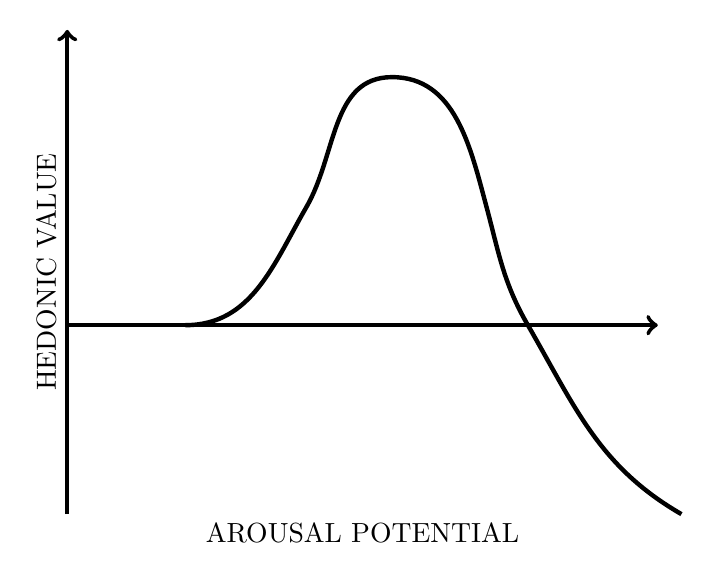
\begin{tikzpicture}[scale=0.75]
      % The image, for reference
      % \node[anchor=south west,inner sep=0] at (0,0) {\includegraphics[width=\textwidth]{wundt.png}};

      % Axes
      \draw[black,ultra thick,->] (1,0.8) -- (1,  9)   node[midway, above, sloped] {HEDONIC VALUE};     % y axis
      \draw[black,ultra thick,->] (1,4)   -- (11, 4);                                                   % x axis
      \path                       (1,0.8) -- (11, 0.8) node[midway, below]         {AROUSAL POTENTIAL}; % x axis label

      % Curve. The numbers come from tracing over wundt.png
      \draw[black,ultra thick] (3, 4)
           to[out=0,   in=240] (5.05, 6)
           to[out=60,  in=180] (6.5,  8.2)
           to[out=0,   in=105] (8.1,  6)
           to[out=-75, in=120] (8.8,  4)
           to[out=-60, in=150] (11.4, 0.8);

      % This version is closer, but a little jagged
      \iffalse
      \draw[black,ultra thick] (3, 4)
           to[out=0,   in=240] (5.05, 6)
           to[out=60,  in=225] (6,    8)
           to[out=45,  in=180] (6.5,  8.2)
           to[out=0,   in=135] (7.2,  8)
           to[out=-45, in=105] (8.1,  6)
           to[out=-75, in=120] (8.8,  4)
           to[out=-60, in=150] (11.4, 0.8);
      \fi
  \end{tikzpicture}

  \caption{The Wundt curve, reproduced from \citep{berlyne1970novelty}. The axes ``hedonic value'' and ``arousal potential'' are described as covering \textquote{reward value\dots preference or pleasure}, and \textquote{all the stimulus properties that tend to raise arousal, including novelty and complexity}, respectively.}

  \label{wundt}
\end{figure}

\emph{Artificial curiosity} (AC) describes active learning systems which are rewarded based on how interesting the input or data they discover is \citep{schmidhuber2006developmental}. Although framed in the context of \emph{reinforcement learning}, this is clearly relevant to our theory exploration setting.

As an unsupervised learning task, AC has no access to labels or meanings associated with its input; the only features it can learn are the structure and relationships inherent in the data, which is very much what we would like a theory exploration system to do. The unifying principle of AC methods is to force systems away from inputs which are not amenable to learning; either because they are so familiar that there is nothing left to learn, or so unfamiliar that they are unintelligible. The resulting behaviour is characterised by the \emph{Wundt curve} (shown in figure \ref{wundt}) \footnote{In practice, many measures avoid negative values for simplicity, in which cases we replace all negative points on the curve with zero.}, which has been used in psychology to explain human aesthetics and preferences \citep{berlyne1970novelty}.

We can divide AC approaches into two groups: the first, which we call \emph{explicit}, send inputs which follow a Wundt curve to their learning algorithm; the second, the \emph{implicit} approaches, instead modify the \emph{output} of their learning algorithm(s), such that the overall system follows a Wundt curve as an emergent property.

In the explicit case, the \emph{implicit reward} signals being learned are analogous to our notion of interestingness. A framework encompassing many examples is given in \citep{oudeyer2007intrinsic} in the context of reinforcement learning.

One particularly general measure is \emph{compression progress}: given a compressed representation of our previous observations, the ``progress'' is the space saved if we include the current observation. Observations which are incompressible or trivially compressible don't save any space, whilst observations which provide new information relevant to past experience can provide a saving. This can be translated to a theorem proving context very naturally: our observations are theorems and their proofs, whilst new theorems which generalise known results will allow us to compress their proofs.

% TODO: Examples
\citep{Schmidhuber1999}

Two sources of intrinsic reward are proposed in \citep{Hester.Stone:2012} for \emph{random forests}. A random forest is a population of decision trees, where each tree is trained on a sub-set of the available examples, each decision is made using a sub-set of the available features, and the predictions of every tree are averaged to obtain that of the forest \citep{randomforests}. The first intrinsic reward is the \emph{disagreement} between predictions; for a forest with $m$ models (trees), predicting features $x_1$ \dots $x_n$ of the state resulting from taking action $a$ in state $s$, we simply sum the Kullback-Leibler divergence $D_{\rm KL}$ of each prediction $P_1$ \dots $P_m$ from every other prediction:

\begin{equation}
  D(s,a) = \sum_{i = 1}^n \sum_{j = 1}^m \sum_{k = 1}^m D_{KL}(P_j(x_i|s,a) || P_k(x_i|s,a))
\end{equation}

$D(s,a)$ is an explicit AC reward, as it follows a Wundt curve as the complexity of transitions increases. For parts of the state space which have been fully learned, the models will agree on accurate predictions. For parts which are unlearnable, the models cannot infer any structure, and will converge to reporting the average of past observations; these predictions may not be accurate, but they will be in agreement. Hence it is the states which are amenable to learning which produce the largest disagreement.

The second intrinsic reward is simply a measure of distance from previous observations, which pushes the system towards unseen states regardless of how learnable they are (similar to the $R_{max}$ technique). This is too simple to meet our definition of AC, but it does force the models to generalise their predictions to unexplored states, acting to increase disagreement in the forest.

A key advantage of random forests is that their models are \emph{inspectable}: they not only give predictions, but also \emph{reasons} for those predictions (i.e. we can see which paths are taken through each decision tree). % TODO: The accuracy of these random forest models are compared

% TODO
\citep{Kaplan2006}
\citep{Lipson2007}
\citep{Luciw2011}
\citep{Macedo2000}
\citep{Ramik.Sabourin.Madani:2013}
\citep{Roa.Kruijff.Jacobsson:2009}
\citep{Schaul.Sun.Wierstra.ea:2011}
\citep{Schmidhuber1999}
\citep{Schmidhuber:1991}
\citep{Scott1989}
\citep{Steunebrink.Koutnik.Thorisson.ea:2013}
\citep{maher2008achieving}
\citep{meyer1991possibility}
\citep{oudeyer2004intelligent}
\citep{oudeyer2014evolution}
\citep{schmidhuber2006developmental}

% TODO: Coevolution

Whilst clearly of relevance to theory exploration, artificial curiosity is usually framed in the context of a \emph{reinforcement learning} and \emph{intrinsic reward}, especially in the field of developmental robotics. This requires non-trivial choices to be made in deciding which of its concepts are of relevance to our domain, and how they may be translated across. For example, much of developmental robotics studies continuous, real-valued sensorimotor signals which may not have any direct analogue in the manipulation of logical formulae. However, if we take a higher-level view, the study of such signals may provide insight for predicting and tuning the behaviour of off-the-shelf ATP algorithms.

The most obvious contrast between developmental robotics and theory exploration is that the latter is not physically embodied (e.g. in a robot). Embodiment has been proposed as a necessary property of intelligent systems, as it provides \emph{grounding} \citep{anderson2003embodied}. Embodiment emerged as a response to the symbolic techniques of GOFAI, and in this sense the fields of theory exploration and developmental robotics seem incompatible. Nevertheless, TE can be seen to avoid the problems of GOFAI in two ways:

\begin{itemize}

  \item Firstly, the abstract, mathematical domain being explored is not a \emph{model} of some external, physical environment; the domain \emph{is} our environment; hence there is no issue of grounding terms with some external meaning.

  \item Secondly, there is a physical aspect of TE in that \emph{resource usage} is a critical factor. If it weren't, then brute force enumeration of proofs would be a viable solution. In this sense, we can provide physical inputs to our algorithms, such as measures of time and space used.

\end{itemize}

\iffalse

\subsubsection{Universal Drives}

PhysRevLett.110.168702.pdf
Omohundro? Too physical.
\emph{Universal drives} are those

\fi

\subsection{Statistics of Formal Systems}

The core problem of assigning ``interestingness'' to logical formulae is the application of statistical reasoning to the discrete, semantically-rich domain of formal systems. This problem has been tackled from various directions for a variety of reasons; here we summarise those contributions which seem of particular importance for theory exploration.

\subsubsection{Relevance Filtering}
\label{relevance}

% TODO
\citep{kuhlwein2012overview}

The combinatorial nature of formal systems causes many proof search methods, such as resolution, to have exponential complexity \citep{haken1985intractability}; hence even a modest size increase can turn a trivial problem into an intractable one. Finding efficient alternatives for such algorithms, especially those which are NP-complete (e.g. determining satisfiability) or co-NP-complete (e.g. determining tautologies), seems unlikely, as it would imply progress on the famously intractable open problems of $\text{P} = \text{NP}$ and $\text{NP} = \text{co-NP}$. On the other hand, we can turn this difficulty around: a modest \emph{decrease} in size may turn an intractable problem into a solvable one. We can ensure that the solutions to these reduced problems coincide with the original if we only remove \emph{redundant} information. This leads to the idea of \emph{relevance filtering}.

Relevance filtering simplifies a proof search problem by removing from consideration those clauses (axioms, definitions, lemmas, etc.) which are deemed \emph{irrelevant}. The technique is used in Sledgehammer during its translation of Isabelle/HOL theories to statements in first order logic: rather than translating the entire theory, only a sub-set of relevant clauses are included. This reduces the size of the problem and speeds up the proof search, but it creates the new problem of determining when a clause is relevant: how do we know what will be required, before we have the proof?

The initial approach, known as \textsc{MePO} (from \emph{Meng-Paulson} \citep{meng2009lightweight}), gives each clause a score based on the proportion $m / n$ of its symbols which are ``relevant'' (where $n$ is the number of symbols in the clause and $m$ is the number which are relevant). Initially, the relevant symbols are those which occur in the goal, but whenever a clause is found which scores more than a particular threshold, all of its symbols are then also considered relevant. There are other heuristics applied too, such as increasing the score of user-provided facts (e.g. given by keywords like \texttt{using}), locally-scoped facts, first-order facts and rarely-occuring facts. To choose $r$ relevant clauses for an ATP invocation, we simply order the clauses by decreasing score and take the first $r$ of them.

Recently, a variety of alternative algorithms have also been investigated, including:

\begin{description}

  \item{\textsc{MaSH}}: Machine Learning for SledgeHammer \citep{kuhlwein2013mash}. The distinguishing feature of \textsc{MaSH} is its use of ``visibility'', which is essentially a dependency graph of which theorems were used in the proofs of which other theorems; although theorems are represented as abstract sets of features. To select relevant clauses for a goal, the set of clauses which are visible from the goal's components is generated; this is further reduced by (an efficient approximation of) a naive Bayes algorithm.

  \item{\textsc{MOR}}: \emph{Multi-output ranking} uses a support vector machine (SVM) approach for selecting relevant axioms from the Mizar Mathematical Library for use by the Vampire ATP system \citep{alama2014premise}. \iffalse TODO: describe the kernel, as that's the interesting bit \fi It compares favourably to \textsc{SNoW} and \textsc{SInE}.

  % TODO:
  \item{\textsc{SInE}}
  \item{\textsc{BliStr}}
  \item{\textsc{HOLyHammer}}
  \item{\textsc{MoMM}}
  \item{\textsc{SNoW}}
  \item{\textsc{MPTP 0.2}}
  \item{\textsc{MaLARea}}
  \item{\textsc{MaLARea SG1}}

\end{description}

\subsubsection{Clustering}
\label{clustering}

% TODO: ML4PG
\citep{journals/corr/abs-1212-3618}
% TODO: ACL2(ml) (also examples section)
\citep{heras2013proof}

\subsubsection{Probability of Sentences}

The most important property of a logical formula is its truth value. Although we may be able to determine some truth values exactly, e.g. using decision or semi-decision procedures, it may be more efficient to \emph{approximate} truth values. One straightforward extension of truth values is \emph{probabilities}, where we can assign probability $1$ to formulae which are known to be true, $0$ to formulae known to be false, and intermediate values to those which we do not yet know.

% TODO
\citep{Hutter.Lloyd.Ng.ea:2013}

\subsubsection{Interestingness in Concept Formation}
\label{conceptformation}

% TODO:
\citep{Montano-Rivas.McCasland.Dixon.ea:2012}
\citep{Piantadosi.Tenenbaum.Goodman:2012}
\citep{Wille:2005}
\citep{colton1999automatic}
\citep{colton2000agent}
\citep{colton2012automated}
\citep{lenat1977automated}
\citep{mullerunderstanding}
\citep{Bundy.Cavallo.Dixon.ea:2015}
\citep{johansson2009isacosy}
\citep{spector2008genetic}
\citep{colton2012automated}
 \citep{geng2006interestingness}
% TODO: How does https en.wikipedia.org/wiki/Discovery system relate?

% However, this search space grows exponentially in the length of the proofs, which is unfortunate since proof length has been proposed as an approximate measure of how interesting a theorem is \cite[\S~10.2.1]{colton2012automated}.

% Alan Bundy et al

% Eurisko, AM, etc.?

\subsubsection{Learning From Structured Data}

One major difficulty with formal mathematics as a domain in which to apply statistical machine learning is the use of \emph{structure} to encode information in objects. In particular, \emph{trees} appear in many places: from inductive datatypes, to recursive function definitions; from theorem statements, to proof objects. Such nested structures may extend to arbitrary depth, which makes them difficult to represent with a fixed number of features, as is expected by most machine learning algorithms. Here we review a selection of solutions to this problem, and compare their distinguishing properties.


\paragraph{Truncation and Padding}

The simplest way to limit the size of our inputs is to truncate anything larger than a particular size (and pad anything smaller). This is the approach taken by ML4PG \citep{journals/corr/abs-1302-6421}, which limits itself to trees with at most 10 levels and 10 elements per level; each tree is converted to a $30 \times 10$ matrix (3 values per tree node) and learning takes place on these normalised representations.

Truncation is unsatisfactory in the way it balances \emph{data} efficiency with \emph{time} efficiency. Specifically, truncation works best when the input data contains no redundancy and is arranged with the most significant data first (in a sense, it is ``big-endian''). The less these assumptions hold, the less we can truncate. Since many ML algorithms scale poorly with input size, we would prefer to eliminate the redundancy using a more aggressive algorithm, to keep the resulting feature size as low as possible.

\paragraph{Dimension Reduction}

A more sophisticated approach to the problem of reducing input size is to view it as a \emph{dimension reduction} technique: our inputs can be modelled as points in high-dimensional spaces, which we want to project into a lower-dimensional space ($\left\{ {0, 1} \right\}^N$ in the case of $N$-bit vectors).

Truncation is a trivial dimension reduction technique: take the first $N$ coordinates (bits). More sophisticated projection functions consider the \emph{distribution} of the points, and project with the hyperplane which preserves as much of the variance as possible (or, equivalently, reduces the \emph{mutual information} between the points).

There are many techniques to find these hyperplanes, such as \emph{principle component analysis} (PCA) and \emph{autoencoding}; however, since these techniques are effectively ML algorithms in their own right, they suffer some of the same constraints we're trying to avoid:

\begin{itemize}
  \item They operate \emph{offline}, requiring all input points up-front
  \item All input points must have the same dimensionality
\end{itemize}

In particular, the second constraint is precisely what we're trying to avoid. Sophisticated dimension reduction is still useful for \emph{compressing} large, redundant features into smaller, information-dense representations, and as such provides a good complement to truncation.

The requirement for offline ``batch'' processing is more difficult to overcome, since any learning we perform for feature extraction will interfere with the core learning algorithm that's consuming these features (this is why deep learning is often done greedily).

\paragraph{Sequencing}

The task of dimension reduction changes when we consider \emph{structured} data. Recursive structures, like trees and lists, have \emph{fractal} dimension: adding layers to a recursive structure gives us more \emph{fine-grained} features, rather than \emph{orthogonal} features. For data mining context-free languages (e.g. those of programming and theorem-proving systems), we will mainly be concerned with tree structures of variable size.

Any investigation of variable-size input would be incomplete without mentioning \emph{sequencing}. This is a lossless approach, which splits the input into fixed-size \emph{chunks}, which are fed into an appropriate ML algorithm one at a time. The sequence is terminated by a sentinel; an ``end-of-sequence'' marker which, by construction, is distinguishable from the data chunks. This technique allows us to trade \emph{space} (the size of our input) for \emph{time} (the number of chunks in a sequence).

Not all ML algorithms can be adapted to accept sequences. One notable approach is to use \emph{recurrent ANNs} (RANNs), which allow arbitrary connections between nodes, including cycles. Compared to \emph{feed-forward} ANNs (FFANNs), which are acyclic, the \emph{future output} of a RANN may depend arbitrarily on its \emph{past inputs} (in fact, RANNs are universal computers).

The main problem with RANNs, compared to the more widely-used FFANNs, is the difficulty of training them. If we extend the standard backpropagation algorithm to handle cycles, we get the \emph{backpropagation through time} algorithm \citep{werbos1990backpropagation}. However, this suffers a problem known as the \emph{vanishing gradient}: error values decay exponentially as they propagate back through the cycles, which prevents effective learning of delayed dependencies, undermining the main advantage of RANNs. The vanishing gradient problem is the subject of current research, with countermeasures including \emph{neuroevolution} (using evolutionary computation techniques to train an ANN) and \emph{long short-term memory} (LSTM; introducing a few special, untrainable nodes to persist values for long time periods \citep{hochreiter1997long}).

The application of \emph{kernel methods} to structured information is discussed in \citep{Gartner2003}, where the input data (including sequences, trees and graphs) are represented using \emph{generative models}, such as hidden Markov models, of a fixed size.

% TODO
\citep{Gartner2003}
\citep{Oveisi.Oveisi.Erfanian.ea:2012}
\citep{bakir2007predicting}
\citep{conf/ijcai/Plate91}
\citep{goller1996learning}
\citep{kwasny1995tail}
\citep{pollack1990recursive}
\citep{zanzotto2012distributed}

\iffalse

Machine learning over structured data:
1D is common: parsing natural language
2D is common; images
Trees are fractal
Backpropagation through structure
LSTM with recursive structure
Most work tries to identify structure; we already have it

Recurrent neural networks
Backpropagation through structure

\fi

\subsection{Interactive Theorem Proving}
\label{itp}

ITP is based around a \emph{proof checker} $C$, which is a decision procedure for determining if a given value $P$ (known as a \emph{proof object} or \emph{witness}) consititutes a proof of a given statement $S$:

$$ C \colon (P \times S) \rightarrow Boolean $$

The process of ITP can hence be understood as the search for an appropriate $P$ for our \emph{goal} $S$:

$$ ITP \colon (S \times C) \rightarrow \{ P \mid C(P, S) = True \} $$

It just so happens that a useful way to implement such a system is via pure functional programming, with the result that many ITP systems (AKA \emph{proof assistants}) such as Coq and Agda appear very similar to languages like Haskell. In particular, we can represent statements $S$ as types and proofs $P$ as values, in which case the proof checker $C$ is simply a type-checker. There are some obvious quirks, such as the need to be \emph{total} (not Turing-complete) in order to ensure soundness, but overall many of the features we introduced for Haskell, such as parametricity, type classes and ADTs are directly translatable to the ITP setting.

This coincidence is due to the \emph{Curry-Howard correspondence} \citep{wadler2015propositions}, which identifies programming languages with systems of logic. Functional programming languages correspond to intuitionistic logics, and are hence a natural fit for reasoning on computers. With additional axioms, we can extend these to more familiar classical logics, although these can make it harder to compute.

Most differences between functional programming and ITP stem from different \emph{expectations} of the user. In the case of Haskell, the desire for expressivity outweighs the desire for soundness, and hence its designers opted to make it Turing-complete. For an ITP language like Agda, soundness far outweighs the inconvenience of having to prove termination, so the opposite tradeoff is made. Similarly, since many ITP ``programs'' (proofs) will never be executed, the language can avoid optimisation in favour of simplicity (and hopefully correctness). This approach is summed up by the \emph{de Bruijn criterion}, which requires that the system \textquote{generates 'proof-objects' (of some form) that can be checked by an 'easy' algorithm} \cite[\S~2]{barendregt2001proof}. One nice consequence of this approach, which is followed for example by Isabelle \citep{nipkow2002isabelle} and Coq \citep{bertot2013interactive}, is that the proof assistants themselves can become arbitrarily complex and even buggy, yet as long as the proof checker remains simple we can maintain a high degree of confidence in the results.

Their emphasis on \emph{interactivity}, mostly caused by operating in undecidable domains, means ITP can require an enormous effort for non-trivial proof or verification tasks (e.g. see \citep{hales2015formal}). One common way to mitigate this problem is by implementing powerful \emph{tactics}: meta-programs which automate as much of a proof as possible. The most striking example of such meta-programming is the \emph{Sledgehammer} component of Isabelle/HOL \citep{journals/iandc/MengQP06}, which invokes a multitude of ATP systems on (a translated form of) the current goal to see if any can provide a proof which Isabelle's core checker will accept.

\subsection{Automated Theorem Proving}
\label{atp}

ATP systems are similar in principle to proof assistants, but are based around a \emph{proof search} algorithm rather than a proof checker. By using a fixed algorithm for proving, such as \emph{resolution} \cite[\S~9.6]{Russell:2003:AIM:773294} or \emph{superposition} \citep{bachmair1994rewrite}, ATP programs are limited to particular decidable or semi-decidable fragments of logic. In particular, most ATP systems (such as E \citep{schulz2013system} and Vampire \citep{riazanov2003implementing}) operate in classical first-order logic. This is the most striking difference from ITP systems (e.g. Coq, Agda and Isabelle) which operate in higher-order logics.

In addition to its interest to logicians, ATP has been actively researched in the field of artificial intelligence, dating back to the founding of the field at the 1956 Dartmouth conference. Even by that time Newell and Simon had developed their Logic Theory Machine \citep{newell1956logic}, which was subsequently able to prove theorems like those in Principia Mathematica \citep{newell1958elements}. The approaches now known as \emph{good old-fashioned AI} (GOFAI) were due in part to the success of automated theorem proving, as attempts were made to formulate many problems in a way amenable to these powerful first-order reasoners.

Recently there has been a trend away from this direction, towards statistical formulations amenable to machine learning, which we will review in \S \ref{related}.

\section{Future Work}
\label{sec:future}

Our use of clustering to pre-process \quickspec{} signatures has required many
decisions and tradeoffs to be made. Hence our approach is just one possibility
out of many alternatives which could be investigated to push this work
further. In addition, there are other ways in which machine learning could aid
theory exploration besides our relevance filter technique. Below, we elaborate
on the details, background and motivation for these choices.

\subsection{Clustering Extensions}
\label{sec:preprocessing}

The most glaring omission in our algorithm is its disregard for types. By
ignoring types, not only are we losing valuable information about expressions,
but we also lose the ability to distinguish between constructors. This is
because a constructor, like \hs{True} or \hs{Just}, has no internal structure;
it is just a token. The distinguishing features of constructors are their types,
which not only tell us which data type they construct, but also their arity, the
types of their arguments, etc.

Our algorithm closely follows that of ML4PG, which \emph{does} support
types. This is handled by populating matrix cells with tokens \emph{and} their
types. Unfortunately this is more complicated in Haskell than it is in Coq,
since types form a separate part of the language from terms, and we do not have
an interactive Core environment to query for types (unlike ML4PG, which runs
inside the Proof General environment).

One partial solution would be leave most Core expressions without types, but to
include them for non-local identifiers (i.e. globals and constructors), which we
can look up in a database. In fact, our \mlforhs{} framework already includes such
type information in its database, alongside the Core syntax trees. Integrating
this information into our algorithm is the next logical step.

We can also compare the performance of our hand-selected features with
\emph{learned} representations, like those reviewed in
\cite{bengio2013representation}. This may provide an indication of how
important it is to understand the language when identifying salient aspects of
expressions, and how difficult various aspects of it might be to learn.

With more expressive features, it may also be useful to experiment with more
powerful learning algorithms. An interesting possibility is to add a feedback
loop between the theory exploration phase and the clustering phase, to more
directly base the similarity of expressions on whether they (are predicted to)
occur together in equations.

\subsection{Theory Exploration Extensions}

Our current approach is a rather conservative change to the existing theory
exploration approaches, as it is essentially a wrapper around \quickspec{}.
There is potential for more radical changes to be made, which alter the search
process itself.

\subsubsection{Variable Instantiation}

\quickcheck{} is certainly the most popular property checker for Haskell, which
motivates its use in \quickspec{} to instantiate variables to random
values. However, this task of finding type inhabitants has also been solved in
many other ways, which may be worth investigating in place of \quickcheck{} (or
perhaps even as part of an ensemble).

The \smallcheck{} system \cite{runciman2008smallcheck} \emph{enumerates}
values rather than sampling them randomly. Whilst this does not make
\smallcheck{} objectively ``better'' than \quickcheck{}, one major advantage
is that it may use much less memory, as the generated values are built up
incrementally. In contrast, \quickcheck{} may generate very large values; in
particular, generating tree structures na\"{\i}vely can cause them to grow
exponentially. For example, here is a potential generator for \hs{RoseTree}s:

\begin{haskell}
genRoseTree = do f        <- arbitrary
                 subtrees <- listOf genRoseTree
                 return (Node f subtrees)
\end{haskell}

The \hs{listOf genRoseTree} call will return a list of arbitrary length, where
each element is generated by \hs{genRoseTree}. This allows an arbitrary number
of recursive calls to be made for each invocation of \hs{genRoseTree}, which
will quickly exhaust the resources of any machine. Whilst such problems may be
anticipated, or quickly spotted, in a property checking setting, this can be
more difficult for our automated approach. For example, if a type does not have
a generator available, we cannot use a library like \hs{derive} to create one
automatically, as it suffers from this na\"{\i}vity problem.

A relative of \smallcheck{} is \lazysmallcheck{}~\cite{reich2013advances}, which
uses laziness to only produce parts of a datastructure as they are demanded.
This may narrow down our search procedures greatly, especially when predicates
are involved. \quickcheck{} allows predicates to restrict the values it tests
with, and hence allows \emph{conditional} equations to be discovered. However,
its implementation uses a simple rejection sampling technique: values are
generated just as if the predicate were not there, and afterwards are filtered
to reject any which do not satisfy the predicate. This makes it difficult to use
very specific predicates, as it is unlikely that many of our random samples will
exactly match our criteria. On the other hand, \lazysmallcheck{} will focus its
search on exactly those parts of the datastructure which are checked by the
predicate, as those are the parts being forced to evaluate. This makes it much
more likely that we will find values which satisfy the predicate, allowing us to
effectively explore more specific conditional properties.

Other approaches to generating inhabitants include
\djinn{}~\cite{augustsson2005djinn}, which uses a decision procedure for a sub-set of
Haskell types which in particular can generate and apply functions (unlike the
above tools, which generate values ``bottom-up'' from constructors, and only use
functions when they have been explicitly written in a
generator). \mucheck{}~\cite{le2014mucheck} is designed for
\emph{mutation testing}, and contains combinators for altering functions in
common ways (e.g. changing the order of pattern match clauses); whilst not as
exhaustive as the other approaches, mutating existing values in this way is
claimed to yield values which correspond more closely to what a programmer might
write. This is an interesting possibility for focusing theory exploration on to
more ``realistic'' areas of the search space, and hence avoiding some of the
more useless or bizarre expressions that random search and enumeration may
produce.

In fact, the database generated by our \astplugin{} may prove helpful in
generating values, since its type information can be fed to a tool like
\djinn{} to discover chains of function applications for building values,
which would be particularly useful in cases where constructors are private, like
in our email example. This is similar to the \hoogle{} tool, but also offers the
ability to use dependency information to avoid potentially infinite recursion.

The Core syntax trees in our database could also be used to generate theories
for automated theorem provers. \hipspec{} currently uses the GHC API to transform
Core within its own process, however that approach suffers from the problems
described in \S~\ref{sec:astplugin}.

\subsubsection{Interestingness}
\label{sec:interestingness}

If we do succeed in producing a fast theory exploration system, which chooses
productive combinations of terms and finds a large number of properties, we
encounter the problem of managing the output: finding the needles we are
interested in among the haystack of trivialities and coincidences.

This is governed by the ``interestingness'' criteria of the theory exploration
system: what to keep and what to discard, and even what areas of the search
space to prioritise. \quickspec{}'s approach, briefly mentioned in
\S~\ref{sec:theoryexploration}, is very simple: we discard equations which are
direct consequences of others, and keep all the rest. Different, and more
sophisticated notions of interestingness have been widely studied in other
fields, which may be applied in the context of theory exploration.

\paragraph{Concept Formation} \label{sec:conceptformation} \leavevmode \newline

One directly applicable area to consider is \emph{concept formation}, which
considers the (automatic) generation of new definitions and axioms. Unlike
theory exploration, such systems are not constrained by the requirement that
their output be provable, and hence interestingness is an important way to judge
the quality of the results.

Approaches vary, from those which are directly related to theory exploration
(such as the scheme-instantiating approach of
\cite{Montano-Rivas.McCasland.Dixon.ea:2012}, which forms part of a theory
exploration system), to others which are more closely related to theories of
human learning and discovery \cite{Piantadosi.Tenenbaum.Goodman:2012,
  mullerunderstanding}. Those based on finding patterns in data, such as
\cite{Wille:2005}, may be useful in tandem with our expression database, and
the results of value generators like \quickcheck{}.

Since tools like \hipspec{} already call out to third-party automated theorem
provers, and indeed our own \mlforhs{} system uses the external Weka program, there
may also be merit in using external concept formation or conjecture generation
tools (or reimplementations of their ideas), in order to build up more structure
on top of that provided by the code we are exploring. For example, the
approaches taken by AM \cite{lenat1977automated, lenat1979automated}, Graffiti
\cite{delavina2005some, delavina2005graffiti} and HR
\cite{colton1999automatic, colton2000agent} could be used alongside those of
\quickspec{}.

\paragraph{Artificial Curiosity} \label{sec:curiosity} \leavevmode \newline

\begin{figure}
  \centering
  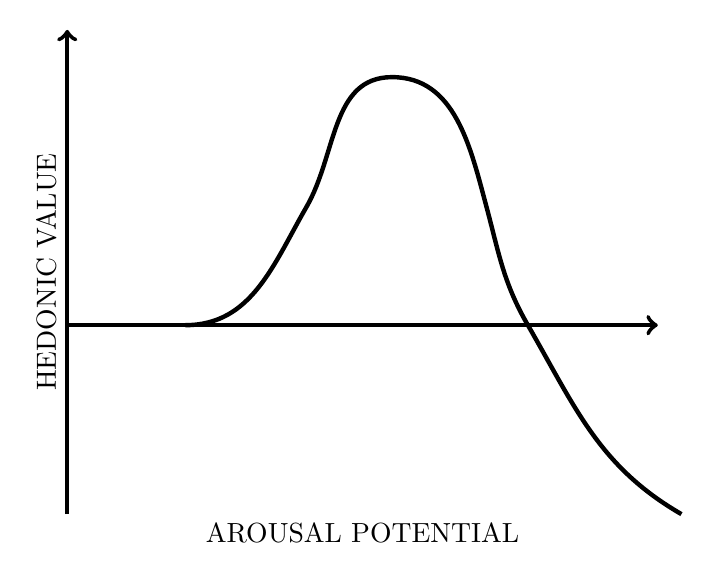
\begin{tikzpicture}[scale=0.75]
      % The image, for reference
      % \node[anchor=south west,inner sep=0] at (0,0) {\includegraphics[width=\textwidth]{wundt.png}};

      % Axes
      \draw[black,ultra thick,->] (1,0.8) -- (1,  9)   node[midway, above, sloped] {HEDONIC VALUE};     % y axis
      \draw[black,ultra thick,->] (1,4)   -- (11, 4);                                                   % x axis
      \path                       (1,0.8) -- (11, 0.8) node[midway, below]         {AROUSAL POTENTIAL}; % x axis label

      % Curve. The numbers come from tracing over wundt.png
      \draw[black,ultra thick] (3, 4)
           to[out=0,   in=240] (5.05, 6)
           to[out=60,  in=180] (6.5,  8.2)
           to[out=0,   in=105] (8.1,  6)
           to[out=-75, in=120] (8.8,  4)
           to[out=-60, in=150] (11.4, 0.8);

      % This version is closer, but a little jagged
      \iffalse
      \draw[black,ultra thick] (3, 4)
           to[out=0,   in=240] (5.05, 6)
           to[out=60,  in=225] (6,    8)
           to[out=45,  in=180] (6.5,  8.2)
           to[out=0,   in=135] (7.2,  8)
           to[out=-45, in=105] (8.1,  6)
           to[out=-75, in=120] (8.8,  4)
           to[out=-60, in=150] (11.4, 0.8);
      \fi
  \end{tikzpicture}

  \caption{The Wundt curve, reproduced from \cite{berlyne1970novelty}. The axes ``hedonic value'' and ``arousal potential'' are described as covering \textquote{reward value\dots preference or pleasure}, and \textquote{all the stimulus properties that tend to raise arousal, including novelty and complexity}, respectively.}

  \label{fig:wundt}
\end{figure}

\emph{Artificial curiosity} (AC) describes active learning systems which are
rewarded based on how interesting the input or data they discover is
\cite{schmidhuber2006developmental}. Although framed in the context of
\emph{reinforcement learning}, this reliance on interest is clearly relevant to
our theory exploration setting.

As an unsupervised learning task, AC has no access to labels or meanings
associated with its input; the only features it can learn are the structure and
relationships inherent in the data, in a similar way to our recurrent clustering
algorithm. The unifying principle of AC methods is to force systems away from
inputs which are not amenable to learning; either because they are so familiar
that there is nothing left to learn, or so unfamiliar that they are
unintelligible. The resulting behaviour is characterised by the \emph{Wundt
  curve} (shown in Figure \ref{fig:wundt}) \footnote{In practice, many measures
  avoid negative values for simplicity, in which cases we replace all negative
  points on the curve with zero.}, which has been used in psychology to explain
human aesthetics and preferences \cite{berlyne1970novelty}. This same behaviour
may be applicable to the theorems produced by a theory exploration system.

We can divide AC approaches into two groups: those which make \emph{explicit}
use of interestingness, learning from signals which follow a Wundt curve; whilst
\emph{implicit} approaches modify the \emph{output} of their learning
algorithm(s), to engineer the overall system behaviour to follow a Wundt curve
as an emergent property.

A framework encompassing many examples of the explicit approach is given in
\cite{oudeyer2007intrinsic} in the context of reinforcement learning; for
comparison, many similar measures are surveyed in a data mining context in
\cite{geng2006interestingness}. Many more reinforcement learning examples can
be found in \cite{Kaplan2006, Lipson2007, Luciw2011, Macedo2000,
  Ramik.Sabourin.Madani:2013, Roa.Kruijff.Jacobsson:2009, Schmidhuber:1991,
  oudeyer2004intelligent}; whilst more general descriptions are given in
\cite{Schaul.Sun.Wierstra.ea:2011, Scott1989, maher2008achieving}, which may be
more amenable to our theory exploration setting.

Many of these reward signals are based on information theory, with a prominent
example being \emph{compression progress}: given a compressed representation of
our previous observations, the ``progress'' is the space saved if we include the
current observation. Observations which are incompressible or trivially
compressible don't save any space, whilst observations which provide new
insights into the structure of past experience can provide a space saving when
compressed together. This seems particularly relevant for our problem of
identifying interesting theorems: those new theorems (``observations'') which
shorten the proofs of previously discovered theorems may be more general, more
powerful and therefore more \emph{interesting} and hence worth keeping. In fact
this is very similar to \quickspec{}'s interestingness criterion.

Another example of explicit artificial curiosity is given in
\cite{Hester.Stone:2012}, where world states which cause \emph{disagreement}
among a population of decision trees (a \emph{random forest}
\cite{randomforests}) are considered interesting. Since the models make
stochastic predictions, the disagreement follows a Wundt curve as the complexity
of state transitions increases: for parts of the state space which have been
fully learned, the models will agree on accurate predictions; for parts which
are unlearnable, the models cannot infer any structure, and will converge to
reporting the same average value. Whilst the latter predictions may not be
\emph{accurate}, they will be \emph{in agreement}, hence pushing down the
interestingness of states which are too complex.

Many examples of the implicit case are based on \emph{coevolution}: rewarding
one part of the system for exploiting another part, and vice versa. In
\cite{Schmidhuber1999} a pair of learning algorithms place virtual ``bets'' on
the outcome of actions, and the winner is rewarded at the expense of the
loser. Due to the risk involved, each algorithm will only bet when it is
confident in its prediction, and bets will only be actioned when each algorithm
is confident in a \emph{different} outcome. The overall behaviour of this system
is therefore similar to the explicit measure of disagreement used in the random
forest example. In terms of theory exploration, such a scheme could be used to
find theorems which are \emph{non-obvious}, and hence informative in some way to
the user.

Another case is the ``darwinian brain'' of Fernando et
al. \cite{fernando2013design1, fernando2013design2}. This coevolves a
population of problem generators and problem solvers, rewarding the solvers
based on their speed, and rewarding the generators based on the \emph{variance}
of the solvers' speed. This avoids trivial problems (which all solvers can
quickly overcome) and complex problems (which no solver can manage), and focuses
on those with the most possibility for learning. It is easy to imagine such a
general architecture being populated by conjecture generators and theorem
provers to form a theory exploration system.

\paragraph{Evolutionary Computation} \leavevmode \newline

Coevolution is a form of \emph{evolutionary computation}; an umbrella term for
heuristic search algorithms which mimic the process of evolution by natural
selection among a population of candidate solutions
\cite{back1997evolutionary}. Whilst \emph{genetic algorithms} are perhaps the
most well-known instance of evolutionary computation, their use of
\emph{strings} to represent solutions causes complications when comparing to a
domain like theory exploration, where recursive structures of unbounded depth
arise. Thankfully these problems are not insurmountable, for example
\emph{genetic programming} can operate on tree-structures natively
\cite{banzhaf1998genetic}, which makes evolutionary computation a useful source
of ideas for reuse in our theory exploration setting (there are also precedents
for using evolutionary computation in a theorem proving domain
\cite{spector2008genetic}).

Traditionally, evolutionary approaches assign solutions a \emph{fitness} value,
using a user-supplied \emph{fitness function}. Fitness should correlate with how
well a solution solves the user's problem; for example, the fitness of a
solution to some engineering problem may depend on the estimated materials
cost. If we frame the task of theory exploration in evolutionary computation
terms, the fitness function would be our interestingness measure.

Pure exploration (i.e. for its own sake) has been studied in evolutionary
computation for two main reasons: \emph{artificial life} and \emph{deceptive
  problems}. The former attempts to gain insight into the nature of life and
biology through competition over limited resources. Whilst this may have utility
in resource allocation, e.g. efficient scheduling of a portfolio of ATP
programs, there is no direct connection to interestingness in theory
exploration, so we will not consider it further (note that similar
resource-usage ideas can also be found in the literature on \emph{artificial
  economies}, e.g. \cite{baum2000evolution}).

On the other hand, work on deceptive problems is highly relevant, as it has lead
to studying various notions of intrinsic fitness, which are analogous to the
interestingness measures we want. Deceptive problems are those where
\textquote{pursuing the objective may prevent the objective from being reached}
\cite{lehman2011abandoning}, which is caused by the fitness (objective)
function having many local optima which are easy to find (e.g. by hill
climbing), but few global optima which are hard to find. Many approaches try to
avoid deception by augmenting the given fitness function to promote
\emph{diversity} and \emph{novelty}, such as \emph{niching methods}
\cite{sareni1998fitness}.

One example is \emph{fitness sharing}, which divides up fitness values between
identical or similar solutions. Say we have a user-provided fitness function
$f$, and a population containing two identical solutions $s_1$ and $s_2$; hence
$f(s_1) = f(s_2)$. In a fitness sharing scheme, we interpret fitness as a fixed
resource, distributed according to $f$; when multiple individuals occupy the
same point in the solution space, they must \emph{share} the fitness available
there. We can describe the fitness \emph{allocated} to a solution by augmenting
$f$, e.g. if we allocate fitness uniformly between identical solutions we get:

$$f'(x) = \frac{f(x)}{\sum_{i=1}^n \delta_{s_i x}}$$

Where $n$ is the population size, $s_i$ is the $i$th solution in the population
and $\delta$ is the Kronecker delta function. In the example above, assuming
there are no other copies in the population, then
$f'(s_1) = \frac{f(s_1)}{2} = \frac{f(s_2)}{2} = f'(s_2)$. By sharing in this
way, the fitness of each solution is balanced against redundancy in the
population: there may still be many copies of a solution, but only when the
fitness is high enough to justify all of them.

There are many variations on this theme, such as sharing between ``close''
solutions rather than just identical ones and judging distance based on fitness
(AKA phenotypically) rather than based on the location in solution space (AKA
genetically). Yet the underlying principle is always the same: penalise
duplication in order to promote diversity. This lesson can be carried over to
our theory exploration context, where a theorem should be considered less
interesting if it is ``close'' to others which have been found.

In a similar way, we can bias our search procedure, rather than our fitness
function, towards diversity. The search procedure in population-based
evolutionary algorithms consists of \emph{selecting} one or more individuals
from the population, e.g. via truncation (select the best $n$ individuals,
discarding the rest); then \emph{transforming} the selected individuals,
e.g. via mutation and crossover, to obtain new solutions.

Traditional selection methods are biased towards high fitness individuals (this
is especially clear for truncation). Alternative schemes have been proposed
which favour diversity \emph{at the expense of} fitness. For example, the
fitness uniform selection scheme (FUSS) \cite{hutter2002fitness} selects a
target fitness $f_t$ uniformly from the interval
$\left[ f_{min}, f_{max} \right]$ between the highest and lowest of the
population. An individual $s$ is then selected with fitness closest to $f_t$,
i.e. $s = \argmin\limits_{x} \lvert f(x) - f_t \rvert$

In this way, the fitness function $f$ is used to assign comparable quantities to
solutions, but it is not treated as the objective; instead, the implicit
objective is to maintain a diverse population, with individuals spread out
uniformly in fitness space. This approach seems useful for informing our work in
theory exploration, as it supports search criteria which \emph{describe}
solutions, but which we may not want to \emph{optimise}. As a simple example, we
might distinguish different forms of theorem by measuring how balanced their
syntax trees are (-1 for left-leaning, +1 for right leaning, 0 for balanced);
but it would be senseless to \emph{maximise} how far they lean.

Once we begin this process of augmenting fitness functions, or abandoning their
use as objectives, an obvious question arises: what happens if our new function
contains nothing of the original? This kind of pure exploration scenario leads
to a variety of ideas for \emph{instrinsic} fitness, such as novelty
\cite{lehman2011abandoning}, which can lead to learning useful ``stepping
stones'' even in objective-driven domains. Such intrinsic notions of fitness are
direct analogues of the interestingness measures we seek for theory exploration.


\end{document}
